\section{Beam Line and Detectors}
\label{hptpcPaper:sec:Methods}

\subsection{Beam Test Overview}
The beam test took place in the T10 beam line, East Area at the Proton Synchrotron in CERN from the 15th August to the 18th September 2018.
The results in this paper use data taken on the 31st August and 1st September, during which the setup configuration was varied as described below.
\todo[inline]{JOCELYN:"really only these two days?  This paper needs to be the flux reference, so we also need to include the flux measurements during the beam test....
suggest cut this sentence in any case and refer to the time ranges of the various types of data where these are analyzed" SEB what do you think?}
The primary components of the  experimental setup for the data taking period are shown schematically in Figure~\ref{fig:setup}.

\begin{figure}
  \includegraphics[width=1.0\linewidth]{files/Figures/hptpc_t10_planview.pdf}
  \caption{Beam test configuration}
  \label{fig:setup}
\end{figure}

\begin{figure}[ht]
  \begin{adjustbox}{max totalsize={.7\textwidth}{.5\textheight},center}
    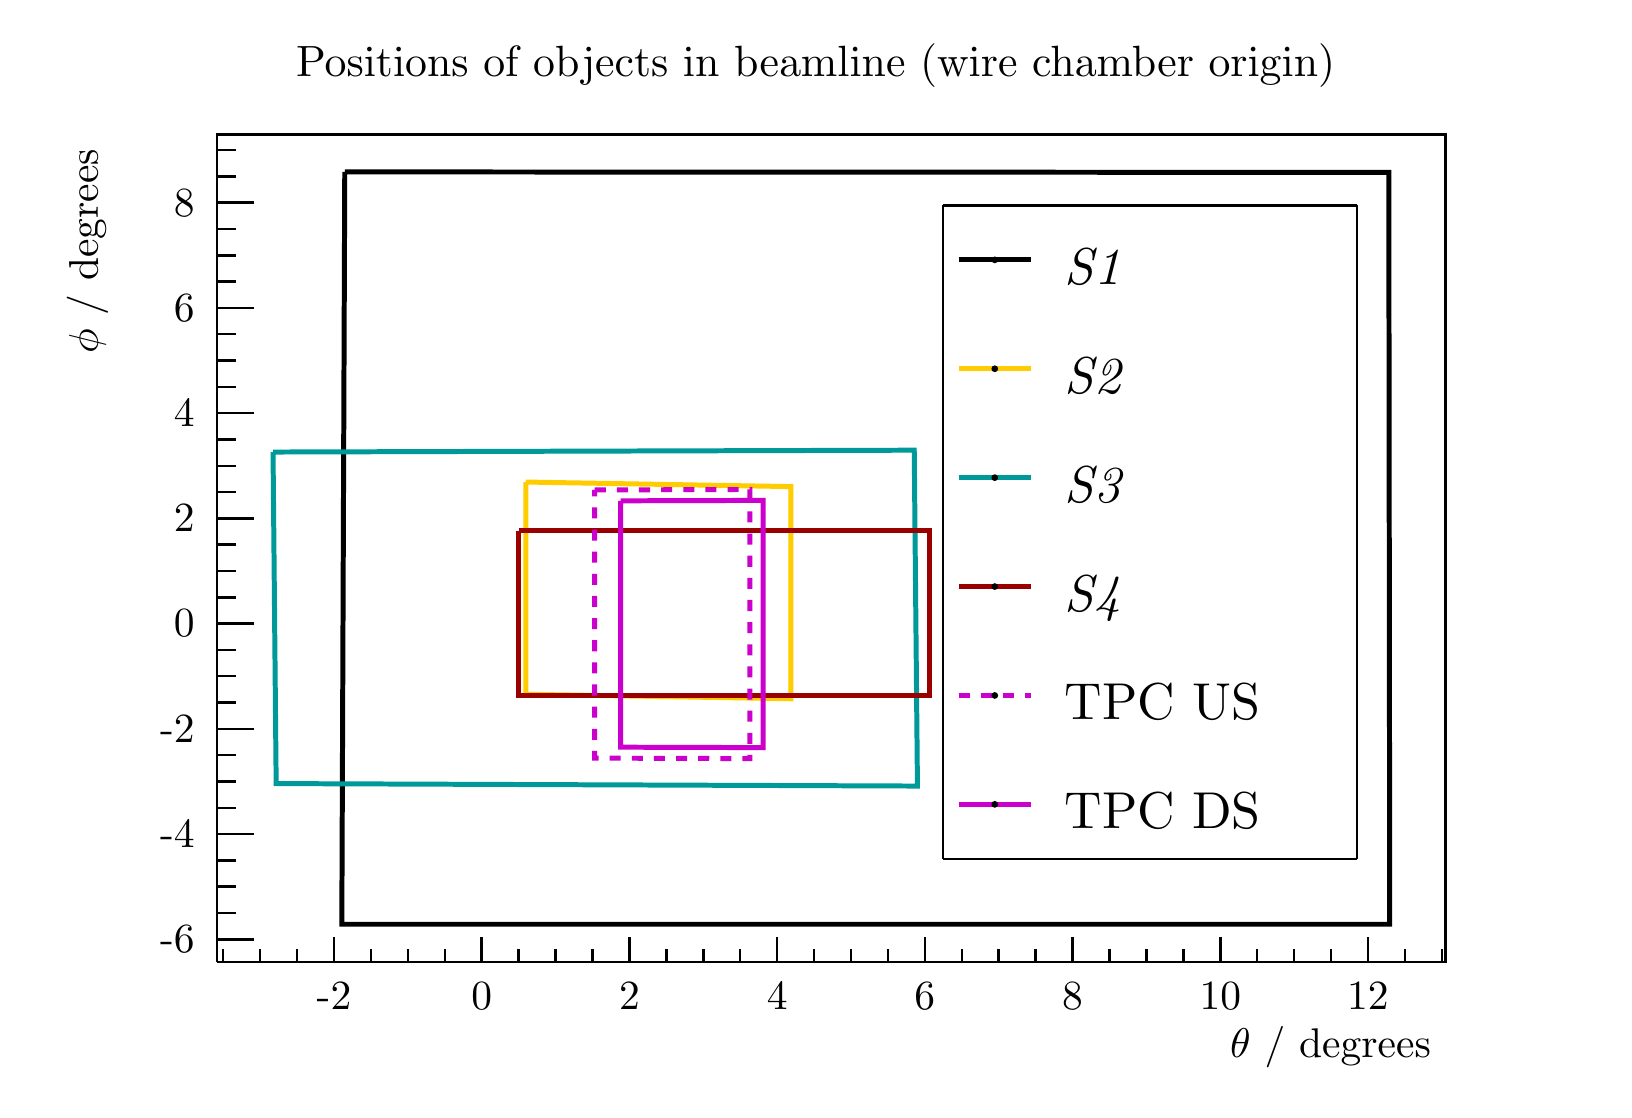
\begin{tikzpicture}
\pgfdeclareplotmark{cross} {
\pgfpathmoveto{\pgfpoint{-0.3\pgfplotmarksize}{\pgfplotmarksize}}
\pgfpathlineto{\pgfpoint{+0.3\pgfplotmarksize}{\pgfplotmarksize}}
\pgfpathlineto{\pgfpoint{+0.3\pgfplotmarksize}{0.3\pgfplotmarksize}}
\pgfpathlineto{\pgfpoint{+1\pgfplotmarksize}{0.3\pgfplotmarksize}}
\pgfpathlineto{\pgfpoint{+1\pgfplotmarksize}{-0.3\pgfplotmarksize}}
\pgfpathlineto{\pgfpoint{+0.3\pgfplotmarksize}{-0.3\pgfplotmarksize}}
\pgfpathlineto{\pgfpoint{+0.3\pgfplotmarksize}{-1.\pgfplotmarksize}}
\pgfpathlineto{\pgfpoint{-0.3\pgfplotmarksize}{-1.\pgfplotmarksize}}
\pgfpathlineto{\pgfpoint{-0.3\pgfplotmarksize}{-0.3\pgfplotmarksize}}
\pgfpathlineto{\pgfpoint{-1.\pgfplotmarksize}{-0.3\pgfplotmarksize}}
\pgfpathlineto{\pgfpoint{-1.\pgfplotmarksize}{0.3\pgfplotmarksize}}
\pgfpathlineto{\pgfpoint{-0.3\pgfplotmarksize}{0.3\pgfplotmarksize}}
\pgfpathclose
\pgfusepathqstroke
}
\pgfdeclareplotmark{cross*} {
\pgfpathmoveto{\pgfpoint{-0.3\pgfplotmarksize}{\pgfplotmarksize}}
\pgfpathlineto{\pgfpoint{+0.3\pgfplotmarksize}{\pgfplotmarksize}}
\pgfpathlineto{\pgfpoint{+0.3\pgfplotmarksize}{0.3\pgfplotmarksize}}
\pgfpathlineto{\pgfpoint{+1\pgfplotmarksize}{0.3\pgfplotmarksize}}
\pgfpathlineto{\pgfpoint{+1\pgfplotmarksize}{-0.3\pgfplotmarksize}}
\pgfpathlineto{\pgfpoint{+0.3\pgfplotmarksize}{-0.3\pgfplotmarksize}}
\pgfpathlineto{\pgfpoint{+0.3\pgfplotmarksize}{-1.\pgfplotmarksize}}
\pgfpathlineto{\pgfpoint{-0.3\pgfplotmarksize}{-1.\pgfplotmarksize}}
\pgfpathlineto{\pgfpoint{-0.3\pgfplotmarksize}{-0.3\pgfplotmarksize}}
\pgfpathlineto{\pgfpoint{-1.\pgfplotmarksize}{-0.3\pgfplotmarksize}}
\pgfpathlineto{\pgfpoint{-1.\pgfplotmarksize}{0.3\pgfplotmarksize}}
\pgfpathlineto{\pgfpoint{-0.3\pgfplotmarksize}{0.3\pgfplotmarksize}}
\pgfpathclose
\pgfusepathqfillstroke
}
\pgfdeclareplotmark{newstar} {
\pgfpathmoveto{\pgfqpoint{0pt}{\pgfplotmarksize}}
\pgfpathlineto{\pgfqpointpolar{44}{0.5\pgfplotmarksize}}
\pgfpathlineto{\pgfqpointpolar{18}{\pgfplotmarksize}}
\pgfpathlineto{\pgfqpointpolar{-20}{0.5\pgfplotmarksize}}
\pgfpathlineto{\pgfqpointpolar{-54}{\pgfplotmarksize}}
\pgfpathlineto{\pgfqpointpolar{-90}{0.5\pgfplotmarksize}}
\pgfpathlineto{\pgfqpointpolar{234}{\pgfplotmarksize}}
\pgfpathlineto{\pgfqpointpolar{198}{0.5\pgfplotmarksize}}
\pgfpathlineto{\pgfqpointpolar{162}{\pgfplotmarksize}}
\pgfpathlineto{\pgfqpointpolar{134}{0.5\pgfplotmarksize}}
\pgfpathclose
\pgfusepathqstroke
}
\pgfdeclareplotmark{newstar*} {
\pgfpathmoveto{\pgfqpoint{0pt}{\pgfplotmarksize}}
\pgfpathlineto{\pgfqpointpolar{44}{0.5\pgfplotmarksize}}
\pgfpathlineto{\pgfqpointpolar{18}{\pgfplotmarksize}}
\pgfpathlineto{\pgfqpointpolar{-20}{0.5\pgfplotmarksize}}
\pgfpathlineto{\pgfqpointpolar{-54}{\pgfplotmarksize}}
\pgfpathlineto{\pgfqpointpolar{-90}{0.5\pgfplotmarksize}}
\pgfpathlineto{\pgfqpointpolar{234}{\pgfplotmarksize}}
\pgfpathlineto{\pgfqpointpolar{198}{0.5\pgfplotmarksize}}
\pgfpathlineto{\pgfqpointpolar{162}{\pgfplotmarksize}}
\pgfpathlineto{\pgfqpointpolar{134}{0.5\pgfplotmarksize}}
\pgfpathclose
\pgfusepathqfillstroke
}
\definecolor{c}{rgb}{1,1,1};
\draw [color=c, fill=c] (0,0) rectangle (20,13.474);
\draw [color=c, fill=c] (2.4,1.61688) rectangle (18,12.1266);
\definecolor{c}{rgb}{0,0,0};
\draw [c,line width=0.9] (2.4,1.61688) -- (2.4,12.1266) -- (18,12.1266) -- (18,1.61688) -- (2.4,1.61688);
\definecolor{c}{rgb}{1,1,1};
\draw [color=c, fill=c] (2.4,1.61688) rectangle (18,12.1266);
\definecolor{c}{rgb}{0,0,0};
\draw [c,line width=0.9] (2.4,1.61688) -- (2.4,12.1266) -- (18,12.1266) -- (18,1.61688) -- (2.4,1.61688);
\draw [c,line width=0.9] (2.4,1.61688) -- (18,1.61688);
\draw [c,line width=0.9] (3.88349,1.93217) -- (3.88349,1.61688);
\draw [c,line width=0.9] (4.35247,1.77452) -- (4.35247,1.61688);
\draw [c,line width=0.9] (4.82145,1.77452) -- (4.82145,1.61688);
\draw [c,line width=0.9] (5.29044,1.77452) -- (5.29044,1.61688);
\draw [c,line width=0.9] (5.75942,1.93217) -- (5.75942,1.61688);
\draw [c,line width=0.9] (6.22841,1.77452) -- (6.22841,1.61688);
\draw [c,line width=0.9] (6.69739,1.77452) -- (6.69739,1.61688);
\draw [c,line width=0.9] (7.16638,1.77452) -- (7.16638,1.61688);
\draw [c,line width=0.9] (7.63536,1.93217) -- (7.63536,1.61688);
\draw [c,line width=0.9] (8.10435,1.77452) -- (8.10435,1.61688);
\draw [c,line width=0.9] (8.57333,1.77452) -- (8.57333,1.61688);
\draw [c,line width=0.9] (9.04231,1.77452) -- (9.04231,1.61688);
\draw [c,line width=0.9] (9.5113,1.93217) -- (9.5113,1.61688);
\draw [c,line width=0.9] (9.98028,1.77452) -- (9.98028,1.61688);
\draw [c,line width=0.9] (10.4493,1.77452) -- (10.4493,1.61688);
\draw [c,line width=0.9] (10.9183,1.77452) -- (10.9183,1.61688);
\draw [c,line width=0.9] (11.3872,1.93217) -- (11.3872,1.61688);
\draw [c,line width=0.9] (11.8562,1.77452) -- (11.8562,1.61688);
\draw [c,line width=0.9] (12.3252,1.77452) -- (12.3252,1.61688);
\draw [c,line width=0.9] (12.7942,1.77452) -- (12.7942,1.61688);
\draw [c,line width=0.9] (13.2632,1.93217) -- (13.2632,1.61688);
\draw [c,line width=0.9] (13.7322,1.77452) -- (13.7322,1.61688);
\draw [c,line width=0.9] (14.2011,1.77452) -- (14.2011,1.61688);
\draw [c,line width=0.9] (14.6701,1.77452) -- (14.6701,1.61688);
\draw [c,line width=0.9] (15.1391,1.93217) -- (15.1391,1.61688);
\draw [c,line width=0.9] (15.6081,1.77452) -- (15.6081,1.61688);
\draw [c,line width=0.9] (16.0771,1.77452) -- (16.0771,1.61688);
\draw [c,line width=0.9] (16.5461,1.77452) -- (16.5461,1.61688);
\draw [c,line width=0.9] (17.015,1.93217) -- (17.015,1.61688);
\draw [c,line width=0.9] (3.88349,1.93217) -- (3.88349,1.61688);
\draw [c,line width=0.9] (3.4145,1.77452) -- (3.4145,1.61688);
\draw [c,line width=0.9] (2.94552,1.77452) -- (2.94552,1.61688);
\draw [c,line width=0.9] (2.47653,1.77452) -- (2.47653,1.61688);
\draw [c,line width=0.9] (17.015,1.93217) -- (17.015,1.61688);
\draw [c,line width=0.9] (17.484,1.77452) -- (17.484,1.61688);
\draw [c,line width=0.9] (17.953,1.77452) -- (17.953,1.61688);
\draw [anchor=base] (3.88349,1.01055) node[scale=1.49939, color=c, rotate=0]{-2};
\draw [anchor=base] (5.75942,1.01055) node[scale=1.49939, color=c, rotate=0]{0};
\draw [anchor=base] (7.63536,1.01055) node[scale=1.49939, color=c, rotate=0]{2};
\draw [anchor=base] (9.5113,1.01055) node[scale=1.49939, color=c, rotate=0]{4};
\draw [anchor=base] (11.3872,1.01055) node[scale=1.49939, color=c, rotate=0]{6};
\draw [anchor=base] (13.2632,1.01055) node[scale=1.49939, color=c, rotate=0]{8};
\draw [anchor=base] (15.1391,1.01055) node[scale=1.49939, color=c, rotate=0]{10};
\draw [anchor=base] (17.015,1.01055) node[scale=1.49939, color=c, rotate=0]{12};
\draw [anchor= east] (18,0.538959) node[scale=1.49939, color=c, rotate=0]{$\theta$ / degrees};
\draw [c,line width=0.9] (2.4,1.61688) -- (2.4,12.1266);
\draw [c,line width=0.9] (2.868,1.90318) -- (2.4,1.90318);
\draw [c,line width=0.9] (2.634,2.2373) -- (2.4,2.2373);
\draw [c,line width=0.9] (2.634,2.57142) -- (2.4,2.57142);
\draw [c,line width=0.9] (2.634,2.90555) -- (2.4,2.90555);
\draw [c,line width=0.9] (2.868,3.23967) -- (2.4,3.23967);
\draw [c,line width=0.9] (2.634,3.57379) -- (2.4,3.57379);
\draw [c,line width=0.9] (2.634,3.90792) -- (2.4,3.90792);
\draw [c,line width=0.9] (2.634,4.24204) -- (2.4,4.24204);
\draw [c,line width=0.9] (2.868,4.57616) -- (2.4,4.57616);
\draw [c,line width=0.9] (2.634,4.91028) -- (2.4,4.91028);
\draw [c,line width=0.9] (2.634,5.24441) -- (2.4,5.24441);
\draw [c,line width=0.9] (2.634,5.57853) -- (2.4,5.57853);
\draw [c,line width=0.9] (2.868,5.91265) -- (2.4,5.91265);
\draw [c,line width=0.9] (2.634,6.24678) -- (2.4,6.24678);
\draw [c,line width=0.9] (2.634,6.5809) -- (2.4,6.5809);
\draw [c,line width=0.9] (2.634,6.91502) -- (2.4,6.91502);
\draw [c,line width=0.9] (2.868,7.24915) -- (2.4,7.24915);
\draw [c,line width=0.9] (2.634,7.58327) -- (2.4,7.58327);
\draw [c,line width=0.9] (2.634,7.91739) -- (2.4,7.91739);
\draw [c,line width=0.9] (2.634,8.25151) -- (2.4,8.25151);
\draw [c,line width=0.9] (2.868,8.58564) -- (2.4,8.58564);
\draw [c,line width=0.9] (2.634,8.91976) -- (2.4,8.91976);
\draw [c,line width=0.9] (2.634,9.25388) -- (2.4,9.25388);
\draw [c,line width=0.9] (2.634,9.58801) -- (2.4,9.58801);
\draw [c,line width=0.9] (2.868,9.92213) -- (2.4,9.92213);
\draw [c,line width=0.9] (2.634,10.2563) -- (2.4,10.2563);
\draw [c,line width=0.9] (2.634,10.5904) -- (2.4,10.5904);
\draw [c,line width=0.9] (2.634,10.9245) -- (2.4,10.9245);
\draw [c,line width=0.9] (2.868,11.2586) -- (2.4,11.2586);
\draw [c,line width=0.9] (2.868,1.90318) -- (2.4,1.90318);
\draw [c,line width=0.9] (2.868,11.2586) -- (2.4,11.2586);
\draw [c,line width=0.9] (2.634,11.5927) -- (2.4,11.5927);
\draw [c,line width=0.9] (2.634,11.9269) -- (2.4,11.9269);
\draw [anchor= east] (2.3,1.90318) node[scale=1.49939, color=c, rotate=0]{-6};
\draw [anchor= east] (2.3,3.23967) node[scale=1.49939, color=c, rotate=0]{-4};
\draw [anchor= east] (2.3,4.57616) node[scale=1.49939, color=c, rotate=0]{-2};
\draw [anchor= east] (2.3,5.91265) node[scale=1.49939, color=c, rotate=0]{0};
\draw [anchor= east] (2.3,7.24915) node[scale=1.49939, color=c, rotate=0]{2};
\draw [anchor= east] (2.3,8.58564) node[scale=1.49939, color=c, rotate=0]{4};
\draw [anchor= east] (2.3,9.92213) node[scale=1.49939, color=c, rotate=0]{6};
\draw [anchor= east] (2.3,11.2586) node[scale=1.49939, color=c, rotate=0]{8};
\draw [anchor= east] (0.753024,12.1266) node[scale=1.49939, color=c, rotate=90]{$\phi$ / degrees};
\draw [c,line width=1.8] (4.02001,11.6489) -- (17.2792,11.643) -- (17.2909,2.09459) -- (3.98258,2.09459) -- (4.02001,11.6489);
\definecolor{c}{rgb}{1,0.8,0};
\draw [c,line width=1.8] (6.32024,7.71036) -- (6.32024,5.01555) -- (9.6851,4.95805) -- (9.6851,7.65257) -- (6.32024,7.71036);
\definecolor{c}{rgb}{0,0.6,0.6};
\draw [c,line width=1.8] (3.10909,8.09147) -- (11.2523,8.11493) -- (11.293,3.84961) -- (3.14872,3.88101) -- (3.10909,8.09147);
\definecolor{c}{rgb}{0.6,0,0};
\draw [c,line width=1.8] (6.22774,7.09184) -- (11.4508,7.09184) -- (11.4508,4.99824) -- (6.22774,4.99824) -- (6.22774,7.09184);
\definecolor{c}{rgb}{0.8,0,0.8};
\draw [c,dash pattern=on 4.00pt off 4.00pt ,line width=1.8] (7.19412,7.60986) -- (9.16463,7.61621) -- (9.16463,4.19793) -- (7.19412,4.20431) -- (7.19412,7.60986);
\draw [c,line width=1.8] (7.52371,7.47197) -- (9.33375,7.47732) -- (9.33375,4.33772) -- (7.52371,4.34311) -- (7.52371,7.47197);
\definecolor{c}{rgb}{0,0,0};
\draw (10,12.9947) node[scale=1.58197, color=c, rotate=0]{Positions of objects in beamline (wire chamber origin)};
\definecolor{c}{rgb}{1,1,1};
\draw [color=c, fill=c] (11.6174,2.92546) rectangle (16.8776,11.2236);
\definecolor{c}{rgb}{0,0,0};
\draw [c,line width=0.9] (11.6174,2.92546) -- (16.8776,2.92546);
\draw [c,line width=0.9] (16.8776,2.92546) -- (16.8776,11.2236);
\draw [c,line width=0.9] (16.8776,11.2236) -- (11.6174,11.2236);
\draw [c,line width=0.9] (11.6174,11.2236) -- (11.6174,2.92546);
\draw [anchor=base west] (12.9325,10.2209) node[scale=1.87424, color=c, rotate=0]{$\mathit{S1}$};
\definecolor{c}{rgb}{1,1,1};
\draw [c, fill=c] (11.8147,10.0481) -- (12.7352,10.0481) -- (12.7352,11.0162) -- (11.8147,11.0162);
\definecolor{c}{rgb}{0,0,0};
\draw [c,line width=1.8] (11.8147,10.5321) -- (12.7352,10.5321);
\foreach \P in {(12.275,10.5321)}{\draw[mark options={color=c,fill=c},mark size=2.402402pt,mark=*,mark size=1pt] plot coordinates {\P};}
\draw [anchor=base west] (12.9325,8.8379) node[scale=1.87424, color=c, rotate=0]{$\mathit{S2}$};
\definecolor{c}{rgb}{1,1,1};
\draw [c, fill=c] (11.8147,8.66503) -- (12.7352,8.66503) -- (12.7352,9.63315) -- (11.8147,9.63315);
\definecolor{c}{rgb}{1,0.8,0};
\draw [c,line width=1.8] (11.8147,9.14909) -- (12.7352,9.14909);
\definecolor{c}{rgb}{0,0,0};
\foreach \P in {(12.275,9.14909)}{\draw[mark options={color=c,fill=c},mark size=2.402402pt,mark=*,mark size=1pt] plot coordinates {\P};}
\draw [anchor=base west] (12.9325,7.45488) node[scale=1.87424, color=c, rotate=0]{$\mathit{S3}$};
\definecolor{c}{rgb}{1,1,1};
\draw [c, fill=c] (11.8147,7.282) -- (12.7352,7.282) -- (12.7352,8.25012) -- (11.8147,8.25012);
\definecolor{c}{rgb}{0,0.6,0.6};
\draw [c,line width=1.8] (11.8147,7.76606) -- (12.7352,7.76606);
\definecolor{c}{rgb}{0,0,0};
\foreach \P in {(12.275,7.76606)}{\draw[mark options={color=c,fill=c},mark size=2.402402pt,mark=*,mark size=1pt] plot coordinates {\P};}
\draw [anchor=base west] (12.9325,6.07185) node[scale=1.87424, color=c, rotate=0]{$\mathit{S4}$};
\definecolor{c}{rgb}{1,1,1};
\draw [c, fill=c] (11.8147,5.89897) -- (12.7352,5.89897) -- (12.7352,6.86709) -- (11.8147,6.86709);
\definecolor{c}{rgb}{0.6,0,0};
\draw [c,line width=1.8] (11.8147,6.38303) -- (12.7352,6.38303);
\definecolor{c}{rgb}{0,0,0};
\foreach \P in {(12.275,6.38303)}{\draw[mark options={color=c,fill=c},mark size=2.402402pt,mark=*,mark size=1pt] plot coordinates {\P};}
\draw [anchor=base west] (12.9325,4.68882) node[scale=1.87424, color=c, rotate=0]{TPC US};
\definecolor{c}{rgb}{1,1,1};
\draw [c, fill=c] (11.8147,4.51594) -- (12.7352,4.51594) -- (12.7352,5.48406) -- (11.8147,5.48406);
\definecolor{c}{rgb}{0.8,0,0.8};
\draw [c,dash pattern=on 4.00pt off 4.00pt ,line width=1.8] (11.8147,5) -- (12.7352,5);
\definecolor{c}{rgb}{0,0,0};
\foreach \P in {(12.275,5)}{\draw[mark options={color=c,fill=c},mark size=2.402402pt,mark=*,mark size=1pt] plot coordinates {\P};}
\draw [anchor=base west] (12.9325,3.30579) node[scale=1.87424, color=c, rotate=0]{TPC DS};
\definecolor{c}{rgb}{1,1,1};
\draw [c, fill=c] (11.8147,3.13291) -- (12.7352,3.13291) -- (12.7352,4.10103) -- (11.8147,4.10103);
\definecolor{c}{rgb}{0.8,0,0.8};
\draw [c,line width=1.8] (11.8147,3.61697) -- (12.7352,3.61697);
\definecolor{c}{rgb}{0,0,0};
\foreach \P in {(12.275,3.61697)}{\draw[mark options={color=c,fill=c},mark size=2.402402pt,mark=*,mark size=1pt] plot coordinates {\P};}
\end{tikzpicture}

  \end{adjustbox}
  \caption{Angular position of various objects within the T10 beamline. US and DS refer to the upstream and downstream faces of the HPTPC. The origin in this view is at the wire chamber (also know as the beam position monitor.}
  \label{fig:angularDist}  
\end{figure}

\begin{table}
  \centering
  \begin{tabular}{|c|c|c|c|c|}
    \hline
    Object & Minimum $\theta$ & Maximum $\theta$ & Minimum $\phi$ & Maximum $\phi$ \\
    \hline
    $\mathit{S1}$ & $-1.89^{\circ} \pm 0.14^{\circ}$ & $12.29^{\circ} \pm 0.14^{\circ}$ & $-5.71^{\circ} \pm 0.14^{\circ}$ & $8.58^{\circ} \pm 0.14^{\circ}$ \\
    $\mathit{S2}$ & $0.60^{\circ}$ \pm 0.02^{\circ} & $4.18^{\circ} \pm 0.02^{\circ}$ & $-1.43^{\circ} \pm 0.02^{\circ}$ & $2.69^{\circ} \pm 0.02^{\circ}$ \\
    $\mathit{S3}$ & $-2.826^{\circ} \pm 0.004^{\circ}$ & $5.900^{\circ} \pm 0.004^{\circ}$ & $-3.087^{\circ} \pm 0.004^{\circ}$ & $3.296^{\circ} \pm 0.004^{\circ}$ \\
    $\mathit{S4}$ & $0.499^{\circ} \pm 0.003^{\circ}$ & $6.068{\circ} \pm 0.003^{\circ}$ & $-1.368{\circ} \pm 0.003^{\circ}$ & $1.765^{\circ} \pm 0.003^{\circ}$ \\
    TPC upstream face & $1.530^{\circ} \pm 0.003^{\circ}$ & $3.630^{\circ} \pm 0.003^{\circ}$ & $-2.566^{\circ} \pm 0.003^{\circ}$ & $2.549^{\circ} \pm 0.003^{\circ}$ \\
    TPC downstream face & $1.881^{\circ} \pm 0.003^{\circ}$ & $3.811^{\circ} \pm 0.003^{\circ}$ & $-2.3567^{\circ} \pm 0.003^{\circ}$ & $2.341^{\circ} \pm 0.003^{\circ}$ \\
    \hline
  \end{tabular}
  \caption{Angular extents of various timing points within the T10 beamline.}
\end{table}

The beam position monitor lies upstream of all the ToF constituents and the TPC, at the beam entrance. 
%The centre of the HPTPC Prototype was placed 13~m from the wire chamber at the beam entrance. 
The beam position monitor is followed by three ToF constituents: $\mathit{S1}$, which provides the trigger is a small-area beam trigger.
$\mathit{S2}$, a trigger counter that provides a coincidence measurement with $\mathit{S1}$.
$\mathit{S3}$, a large wall of plastic scintillator bars, placed directly upstream of the TPC vessel.
All three of these upstream constituents are described in greater detail in Sections~\ref{subsec:s1s2Exp}~and~\ref{subsec:s3Exp}.
Directly between $\mathit{S1}$ and $\mathit{S2}$, a variable number of blocks of acrylic moderator were placed, and are shown in Figure~\ref{fig:modblocks}.
The vessel containing the TPC was placed 13~m from the wire chamber at the beam entrance.
Lastly, a fourth ToF constituent, labeled \textit{S4}, was placed directly downstream of the vessel.
This was a second wall of plastic scintillator bars, described further in Section~\ref{subsec:s4Exp}.
Both the TPC and ToF systems were placed at an off-axis angle with respect to the direction of the beam.
To study the impact of moderator thickness, a variable number of blocks of acrylic, each of dimension $10\times10\times10$~cm$^3$, were placed in the beamline, with the upstream end of the moderators located xxx cm behind \textit{S1}, and are shown in Figure~\ref{fig:modblocks}.

\todo[inline]{also need the off axis angle (with +/-). Need to check the mod block from S1}

Data acquisition (DAQ) of up- and downstream ToF systems were completely independent.
The synchronization between systems was performed offline using the reference signal from the PS at the beginning of every spill.
The PS beam structure is as follows: T10 received between 1 and 3 spills during each supercycle which has a typical duration of 33~s.
The spill duration is approximately 400~ms.
The minimum separation in time between two spills is approximately 1 second.
Therefore the start of spill signal frequency is 1 Hz or smaller.
The trigger condition of the upstream ToF was based on the coincidence between \textit{S1} and \textit{S3} constituents.
\textit{S2} signals were also recorded but the upstream ToF DAQ but were not a trigger condition.
The DAQ of the downstream ToF, \textit{S4}, was run in self-triggering mode with a gate open during the spill.
Coincidence signals between \textit{S1} and \textit{S2} counters were also recorded by the downstream ToF DAQ and were used in the particle identification (PID) analysis, described in Section~\ref{hptpcPaper:sec:Results}.  

A system of moderator blocks was located between the \textit{S1} and \textit{S2} counters.
The system was composed of a stand on which up to four polystyrene $10\times10\times10$~cm$^3$ blocks could be placed contiguously.
Figure~\ref{fig:modblocks} shows the stand with four blocks installed.
The moderator blocks have the effect of both reducing the energy of incoming particles as well as scattering protons in the beam through higher angles than beam MIPs.
This tends to increase in the proton-to-MIP ratio at low off-axis angles from the beam, while decreasing the total number of protons and MIPs traversing the TPC.
A maximum of four moderator blocks was chosen to retain a minimum intensity in the TPC.
%The addition of too many moderator blocks would cause an overscattering whereby too many protons fall below threshold as compared with MIPs.

Data was taken with the beam momentum primarily at 0.8~GeV/c, and with each configuration of 0 to 4 moderator blocks.
Figure~INSERT shows the typical composition of the beam upstream of \textit{S1} at 0.8~GeV/c. Beam spills were approximately 500~ms in length with 5-10~s between spills.  
\todo[inline]{JOCELYN:"In general, you need a paragraph and a figure or two that describe the T10 beam before you do anything to it. The description of the un-modified beam should come before any explanation about the modifications, so probably as a subsection at the end of section 1. This unmodified beam data should probably come from the 2016 measurements, or the on-axis TOF measurements with no moderator." - similar to previous comment 2016 data probably best So maybe remove figure INSERT, and just do a subsection at the end of section 1.}

%    Moderator blocks were used in order to cause a spread in the incoming beam.
%    The blocks cause protons to scatter through a larger angle than pions and other minimum ionising particles (MIP), increasing the off-axis proton pion ratio.
%    The effect of this, together with placing the TPC and ToF systems off axis was to allow a measurement of protons with a lower pion background.
%    This technique also had the effect of reducing the average momentum of the measured particles.
%    Data were taken for 0, 1, 2, 3, and 4 moderator blocks in turn.
%    The beam ran with an energy of 0.8~GeV/c, and primarily comprised protons and pions, as well as muons and electrons. 
%    Beam spills were approximately 500~ms in length, with 5-10~s between spills.
%    The ratio of protons to pions expected in the T10 beam  is shown in figure~\ref{beamcharacteristics}.
%    From this figure, the expected on axis proton pion ratio at 0.8~GeV/c is approximately 1:6.
%      \begin{figure}
%      \centering
%    \includegraphics[width=0.6\linewidth]{files/Figures/offaxismeasurement.png}
%    	\caption{T10 beam constituents (REFERENCE NEEDED)}
%    		\label{fig:beamcharacteristics}
%    \end{figure}


\begin{figure}[t]
  \centering
  %\includegraphics[width=0.2\linewidth]{files/Figures/ModeratorBlocks.jpg}
  \includegraphics[width=1.05\linewidth]{files/Figures/S1S2S3S4.png}
  \caption{Photo demonstrating the \textit{S1} and \textit{S2} counters and the stand with four acrylic moderator blocks of the upstream part of the setup (right). Photo of the downstream part of the setup which shows the \textit{S3}, \textit{S4} detectors and HPTPC (left).}
  \label{fig:modblocks}
\end{figure}

\subsection{Upstream beam counters S1 and S2}
\label{subsec:s1s2Exp}
JOCELYN:"This actually isn't a good picture of S1, need one that shows the hardware head on." (do we have one of these?)
The beam counters \textit{S1} and \textit{S2} are shown in Figure~\ref{fig:modblocks}, right.
The \textit{S1} counter is a $40\times40\times5$~mm$^3$ plastic scintillator cross which is attached to four 1'' Hamamatsu R4998 phototubes at each end for the light readout.
The time resolution of the counter, as measured by the DAQ system of the upstream ToF, was about 30~ps. 
\todo{replace about with an error bar on the 30 ps. JOCELYN:" And even better, include a timing distribution of the S1 data that has FWHM or sigma of 30 ps." SEB do you have any info like this? If not, we will need to talk to ALEXANDER KORZENEV about it.}
\todo{JOCELYN:"for time of flight, distance knowledge is essential.  Need a paragraph before 2.2. that describes how the distances are known (the survey, and description of survey methodology and precision), and includes a table of the relevant distances with error bars."}

The \textit{S2} counter is a scintillator tile of size $120\times120\times5$~mm$^3$, coupled to a 2" PMT R1309, which  2'' PMT R13089 which was connected to the scintillator via long light-guide as shown in Figure~\ref{fig:modblocks}.
The \textit{S2} counter was placed $(1.41 \pm 0.01)~\text{m}$ \todo{THIS NUMBER NEEDS CHECKING - SEB?} downstream of \textit{S1}.
The transverse position of \textit{S2} was adjusted to account for the beam divergence in the moderator blocks.

The analog signals from one of the \textit{S1} PMTs and \textit{S2} PMT were fed into NIM discriminator units.
\todo{JOCELYN:"with what threshold? specify. Was it really only one of the S1 PMTs? I thought a coincidence of the S1 PMTs was formed, and then that signal was ANDed with the S2 PMT." ALEXANDER KORZENEV?}
%set at AA mV and BB mV respectively. 
Subsequently, the discriminated signals were fed into a NIM coincidence unit, and the coincidence of the two signals was recorded by the DAQ systems of the upstream ToF wall (\textit{S3}) and the downstream ToF wall (\textit{S4}). This information was further used for the time-of-flight analysis of the downstream ToF. \todo{JOCELYN:"but not the upstream? why not?" SEB?}


\subsection{Upstream Time of Flight instrumentation (S3)}
\label{subsec:s3Exp}
\todo{JOCELYN:"Replace just upstream with a number and error bar"}
The \textit{S3} `upstream' ToF constituent was placed just upstream of the HPTPC prototype in the beamline.
A schematic drawing of the \textit{S3} ToF wall is shown in Figure~\ref{fig:S3sketch}.
The detector is composed of 22 staggered scintillator bars:  20 bars with dimensions $1.7 \times 6.0 \times 1.0$~cm$^3$ and 2 bars of  $1.5 \times 6.0 \times 1.0$~cm$^3$ placed on top and bottom \cite{S3-proceedings}.
The overlap between bars was set to 5~mm, thus the active area of the detector was approximately 1.68 $\times$ 1.22~m$^2$.
\todo{JOCELYN:"Give exact detector area" - ALEXANDER KORZENEV}
\begin{figure}
  \centering
  \includegraphics[width=0.48\linewidth]{files/Figures/uToF_sketch.pdf}
  \hfill
  \includegraphics[width=0.5\linewidth]{files/Figures/uToF_rot.pdf}
  \caption{Sketch of the \textit{S3} wall \cite{S3-proceedings}.
  Front (left) and rotated (right) views are presented.}
  \label{fig:S3sketch}
\end{figure}
\todo{JOCELYN:"its not clear from this description that the bars are staggered in z, include a side view in Fig. 5 to clarify."- ALEXANDER KORZENEV}
\todo{JOCELYN:"Use cm everywhere, no m or mm"}
The bars are made from the plastic scintillator, EJ-200 \cite{SCIONIX}, which 
provides a suitable optical attenuation length of 4~m and fast timing, with a rise time of 0.9~ns and decay time constant of 2.1~ns.
\todo{JOCELYN:"give the scintillator brightness first (usually in photons per MeV deposited), then the attenuation length " - ALEXANDER KORZENEV}
The scintillation emission spectrum of EJ-200 resides primarily in the violet region of the visible spectrum that corresponds well to the photon detection efficiency wavelength range of photosensors used for the readout. \todo{JOCEYLN: "Add a sentence describing how the bars were wrapped (with what, why, with what reflectivity, etc.)" - ALEXANDER KORZENEV}
\todo{JOCELYN:"give the wavelength range numerically here, and include a citation to the data sheet that shows the spectrum" - ALEXANDER KORZENEV}

Arrays of eight $6 \times 6$~mm$^2$ area silicon photomultipliers (SiPMs) S13360-6050PE from Hamamatsu Photonics \cite{Hamamatsu} were coupled to each end of the bar to collect scintillation photons.
The anode signals of the SiPMs are read out, summed and shaped by a dedicated circuit as described in Ref.\,\cite{S3-readout}.
%an 8-channel SiPM anode readout integrated circuit MUSIC-R1. %The construction of the prototype was a joint effort between groups of Geneva and Zurich universities as a part of R\&D for the Timing detector of the SHIP experiment \cite{AK}.

A 64-ch SAMPIC  module was used for the data acquisition.
A SAMPIC chip is a Waveform and Time to Digital Converter (WTDC) 16-channel ASIC which provides a raw time with an ultrafast analog memory allowing fine timing extraction as well as other parameters of the pulse~\cite{SAMPIC}.
Each channel contains a discriminator that can trigger itself independently or participate in a more complex combined trigger. 
Three module ASICs ($16\times3=48$ channels) were connected to the 44 channels of $\mathit{S3}$ and were operated in self-triggering mode.
\todo{JOCELYN:"What were the conditions of the self trigger i.e. threshold? multiplicity? time over threshold? etc.) specify here." ALEXANDER KORZENEV}
A 4th ASIC was used to acquire data from $\mathit{S1}$, the coincidence signal $\mathit{S1} \cap \mathit{S2}$, and the start-of-spill signal from PS.
A second level trigger was implemented in firmware and run on the level of the ASICs: the data were only sent to the hard disk of the DAQ notebook in the case of coincidence between $\mathit{S1}$ channels and channels of three ASICs used for $\mathit{S3}$.

A mean time of light signals detected at two ends of a single bar provides a time reference with a resolution of about 100~ps, while the difference between the time of the light signals gives the position of the interaction along the bar, with a resolution of 1.6~cm.

Examples of reconstructed $XY$ distributions are shown in Figures~\ref{fig:s3XY_pion} and~\ref{fig:s3XY_proton}.
The axes of the distributions shown in Figures~\ref{fig:s3XY_pion} and~\ref{fig:s3XY_proton} are local coordinates for $\mathit{S3}$ where $y=0~cm$ is the bottom of the active area and $y=120~cm$ is the top of the active area.
In the $x$ direction, 0~cm is the left-hand side of $\mathit{S3}$ as viewed from $\mathit{S1}$, while $x = 170~cm$ is the right-hand edge of $\mathit{S3}$.
Figure~\ref{fig:s3XY_pion} shows the spatial distribution of hits in $\mathit{S3}$ thought to be produced by MIPs when no moderator was present in the beamline.
This distribution shows that most of the hits are concentrated in one small spot of the detector (the beam centre).

Figure~\ref{fig:s3XY_proton} shows the spatial distribution of hits identified in $\mathit{S3}$ as protons when 4 moderator blocks were in the beamline.
In contrast to Figure~\ref{fig:s3XY_pion}, the pattern of hits is far more diffuse.
This clearly shows the scattering effect of the moderator blocks.

\todo{JOCELYN: "to understand whether the axes make sense, the reader needs to know the coordinate system.  The paper needs a paragraph on the coordinates of the upstream TOF somewhere before reconstruction is discussed to make sense of this.  That paragraph should spell out where the TOF is, and where the beam is expected to be, and then the discussion of these figures (that needs to be included in the reconstruction section) should compare the measured beam center position (which can't really be determined from these figures, so the caption should give it, as well as the text), with the expected beam center position." SEB/We will have included the axes in the beam diagram further up.}

\begin{figure}[t]
  \begin{minipage}[t]{0.49\textwidth}
    \centering
    \begin{adjustbox}{max totalsize={\textwidth}{.5\textheight},center}
      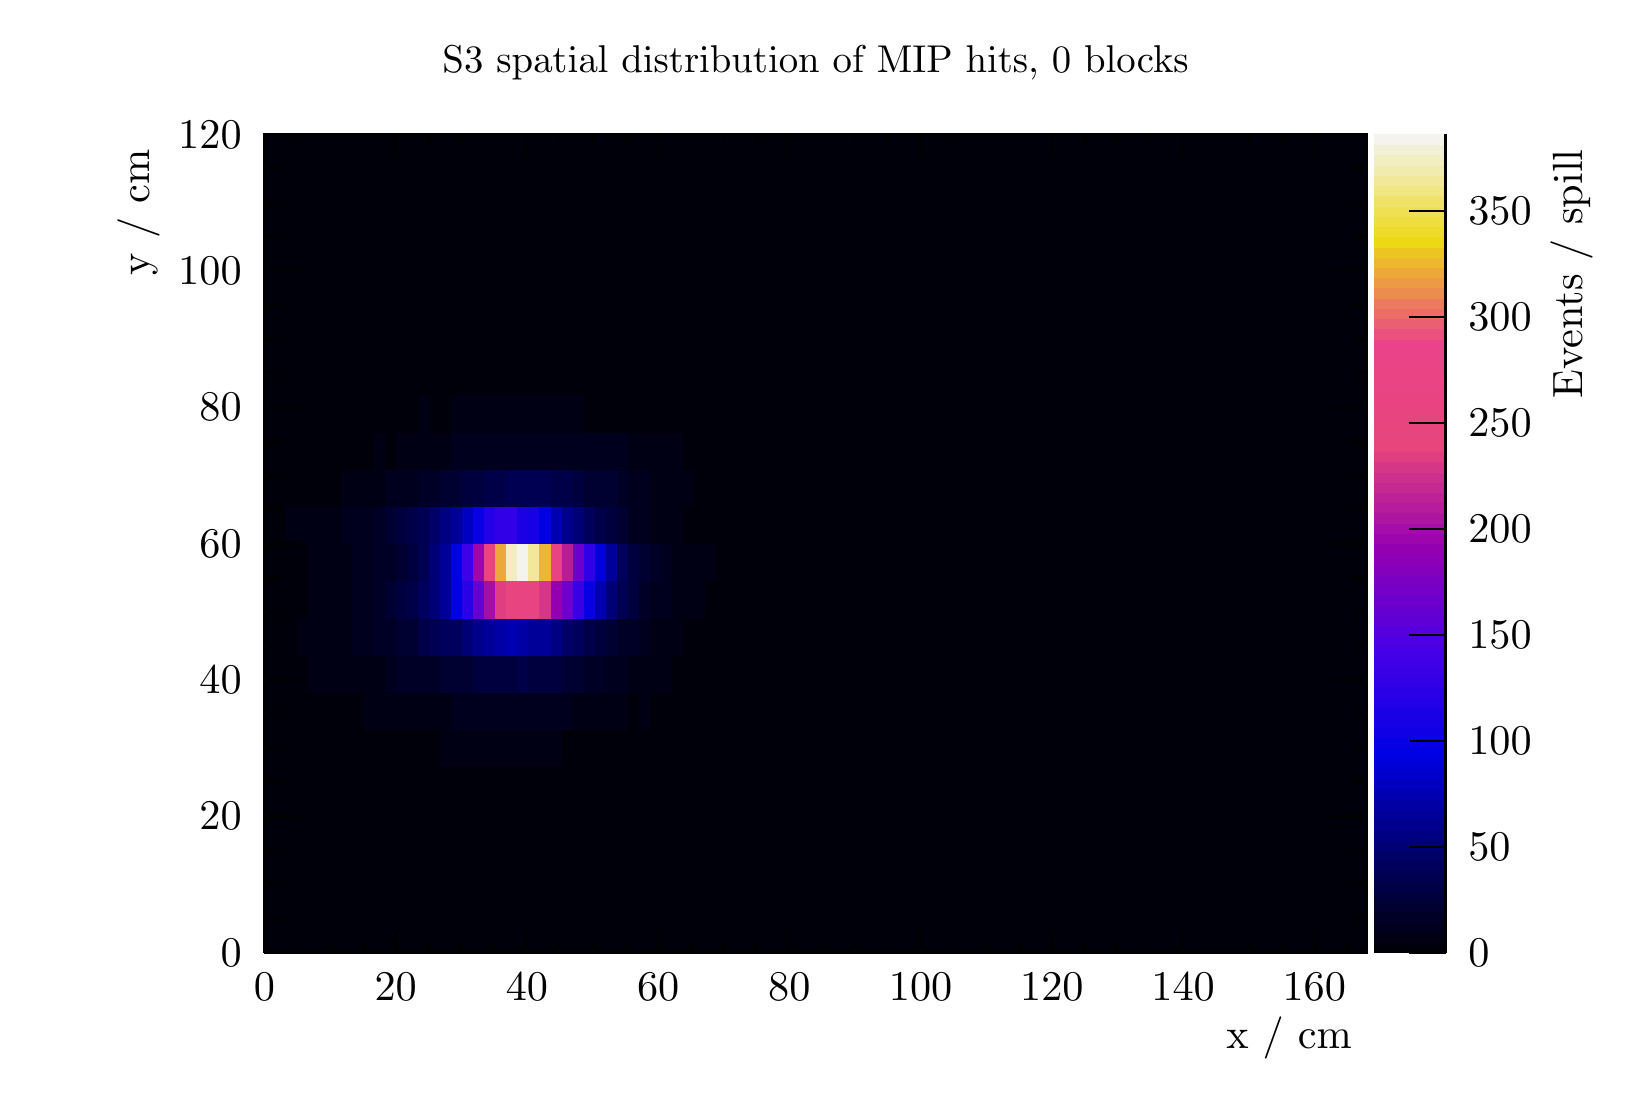
\begin{tikzpicture}
\pgfdeclareplotmark{cross} {
\pgfpathmoveto{\pgfpoint{-0.3\pgfplotmarksize}{\pgfplotmarksize}}
\pgfpathlineto{\pgfpoint{+0.3\pgfplotmarksize}{\pgfplotmarksize}}
\pgfpathlineto{\pgfpoint{+0.3\pgfplotmarksize}{0.3\pgfplotmarksize}}
\pgfpathlineto{\pgfpoint{+1\pgfplotmarksize}{0.3\pgfplotmarksize}}
\pgfpathlineto{\pgfpoint{+1\pgfplotmarksize}{-0.3\pgfplotmarksize}}
\pgfpathlineto{\pgfpoint{+0.3\pgfplotmarksize}{-0.3\pgfplotmarksize}}
\pgfpathlineto{\pgfpoint{+0.3\pgfplotmarksize}{-1.\pgfplotmarksize}}
\pgfpathlineto{\pgfpoint{-0.3\pgfplotmarksize}{-1.\pgfplotmarksize}}
\pgfpathlineto{\pgfpoint{-0.3\pgfplotmarksize}{-0.3\pgfplotmarksize}}
\pgfpathlineto{\pgfpoint{-1.\pgfplotmarksize}{-0.3\pgfplotmarksize}}
\pgfpathlineto{\pgfpoint{-1.\pgfplotmarksize}{0.3\pgfplotmarksize}}
\pgfpathlineto{\pgfpoint{-0.3\pgfplotmarksize}{0.3\pgfplotmarksize}}
\pgfpathclose
\pgfusepathqstroke
}
\pgfdeclareplotmark{cross*} {
\pgfpathmoveto{\pgfpoint{-0.3\pgfplotmarksize}{\pgfplotmarksize}}
\pgfpathlineto{\pgfpoint{+0.3\pgfplotmarksize}{\pgfplotmarksize}}
\pgfpathlineto{\pgfpoint{+0.3\pgfplotmarksize}{0.3\pgfplotmarksize}}
\pgfpathlineto{\pgfpoint{+1\pgfplotmarksize}{0.3\pgfplotmarksize}}
\pgfpathlineto{\pgfpoint{+1\pgfplotmarksize}{-0.3\pgfplotmarksize}}
\pgfpathlineto{\pgfpoint{+0.3\pgfplotmarksize}{-0.3\pgfplotmarksize}}
\pgfpathlineto{\pgfpoint{+0.3\pgfplotmarksize}{-1.\pgfplotmarksize}}
\pgfpathlineto{\pgfpoint{-0.3\pgfplotmarksize}{-1.\pgfplotmarksize}}
\pgfpathlineto{\pgfpoint{-0.3\pgfplotmarksize}{-0.3\pgfplotmarksize}}
\pgfpathlineto{\pgfpoint{-1.\pgfplotmarksize}{-0.3\pgfplotmarksize}}
\pgfpathlineto{\pgfpoint{-1.\pgfplotmarksize}{0.3\pgfplotmarksize}}
\pgfpathlineto{\pgfpoint{-0.3\pgfplotmarksize}{0.3\pgfplotmarksize}}
\pgfpathclose
\pgfusepathqfillstroke
}
\pgfdeclareplotmark{newstar} {
\pgfpathmoveto{\pgfqpoint{0pt}{\pgfplotmarksize}}
\pgfpathlineto{\pgfqpointpolar{44}{0.5\pgfplotmarksize}}
\pgfpathlineto{\pgfqpointpolar{18}{\pgfplotmarksize}}
\pgfpathlineto{\pgfqpointpolar{-20}{0.5\pgfplotmarksize}}
\pgfpathlineto{\pgfqpointpolar{-54}{\pgfplotmarksize}}
\pgfpathlineto{\pgfqpointpolar{-90}{0.5\pgfplotmarksize}}
\pgfpathlineto{\pgfqpointpolar{234}{\pgfplotmarksize}}
\pgfpathlineto{\pgfqpointpolar{198}{0.5\pgfplotmarksize}}
\pgfpathlineto{\pgfqpointpolar{162}{\pgfplotmarksize}}
\pgfpathlineto{\pgfqpointpolar{134}{0.5\pgfplotmarksize}}
\pgfpathclose
\pgfusepathqstroke
}
\pgfdeclareplotmark{newstar*} {
\pgfpathmoveto{\pgfqpoint{0pt}{\pgfplotmarksize}}
\pgfpathlineto{\pgfqpointpolar{44}{0.5\pgfplotmarksize}}
\pgfpathlineto{\pgfqpointpolar{18}{\pgfplotmarksize}}
\pgfpathlineto{\pgfqpointpolar{-20}{0.5\pgfplotmarksize}}
\pgfpathlineto{\pgfqpointpolar{-54}{\pgfplotmarksize}}
\pgfpathlineto{\pgfqpointpolar{-90}{0.5\pgfplotmarksize}}
\pgfpathlineto{\pgfqpointpolar{234}{\pgfplotmarksize}}
\pgfpathlineto{\pgfqpointpolar{198}{0.5\pgfplotmarksize}}
\pgfpathlineto{\pgfqpointpolar{162}{\pgfplotmarksize}}
\pgfpathlineto{\pgfqpointpolar{134}{0.5\pgfplotmarksize}}
\pgfpathclose
\pgfusepathqfillstroke
}
\definecolor{c}{rgb}{1,1,1};
\draw [color=c, fill=c] (0,0) rectangle (20,13.4957);
\draw [color=c, fill=c] (3,1.75444) rectangle (17,12.1461);
\definecolor{c}{rgb}{0,0,0};
\draw [c,line width=0.9] (3,1.75444) -- (3,12.1461) -- (17,12.1461) -- (17,1.75444) -- (3,1.75444);
\definecolor{c}{rgb}{1,1,1};
\draw [color=c, fill=c] (3,1.75444) rectangle (17,12.1461);
\definecolor{c}{rgb}{0,0,0};
\draw [c,line width=0.9] (3,1.75444) -- (3,12.1461) -- (17,12.1461) -- (17,1.75444) -- (3,1.75444);
\definecolor{c}{rgb}{0,0,0.0387097};
\draw [color=c, fill=c] (3,1.75444) rectangle (3.14,2.22679);
\draw [color=c, fill=c] (3.14,1.75444) rectangle (3.28,2.22679);
\draw [color=c, fill=c] (3.28,1.75444) rectangle (3.42,2.22679);
\draw [color=c, fill=c] (3.42,1.75444) rectangle (3.56,2.22679);
\draw [color=c, fill=c] (3.56,1.75444) rectangle (3.7,2.22679);
\draw [color=c, fill=c] (3.7,1.75444) rectangle (3.84,2.22679);
\draw [color=c, fill=c] (3.84,1.75444) rectangle (3.98,2.22679);
\draw [color=c, fill=c] (3.98,1.75444) rectangle (4.12,2.22679);
\draw [color=c, fill=c] (4.12,1.75444) rectangle (4.26,2.22679);
\draw [color=c, fill=c] (4.26,1.75444) rectangle (4.4,2.22679);
\draw [color=c, fill=c] (4.4,1.75444) rectangle (4.54,2.22679);
\draw [color=c, fill=c] (4.54,1.75444) rectangle (4.68,2.22679);
\draw [color=c, fill=c] (4.68,1.75444) rectangle (4.82,2.22679);
\draw [color=c, fill=c] (4.82,1.75444) rectangle (4.96,2.22679);
\draw [color=c, fill=c] (4.96,1.75444) rectangle (5.1,2.22679);
\draw [color=c, fill=c] (5.1,1.75444) rectangle (5.24,2.22679);
\draw [color=c, fill=c] (5.24,1.75444) rectangle (5.38,2.22679);
\draw [color=c, fill=c] (5.38,1.75444) rectangle (5.52,2.22679);
\draw [color=c, fill=c] (5.52,1.75444) rectangle (5.66,2.22679);
\draw [color=c, fill=c] (5.66,1.75444) rectangle (5.8,2.22679);
\draw [color=c, fill=c] (5.8,1.75444) rectangle (5.94,2.22679);
\draw [color=c, fill=c] (5.94,1.75444) rectangle (6.08,2.22679);
\draw [color=c, fill=c] (6.08,1.75444) rectangle (6.22,2.22679);
\draw [color=c, fill=c] (6.22,1.75444) rectangle (6.36,2.22679);
\draw [color=c, fill=c] (6.36,1.75444) rectangle (6.5,2.22679);
\draw [color=c, fill=c] (6.5,1.75444) rectangle (6.64,2.22679);
\draw [color=c, fill=c] (6.64,1.75444) rectangle (6.78,2.22679);
\draw [color=c, fill=c] (6.78,1.75444) rectangle (6.92,2.22679);
\draw [color=c, fill=c] (6.92,1.75444) rectangle (7.06,2.22679);
\draw [color=c, fill=c] (7.06,1.75444) rectangle (7.2,2.22679);
\draw [color=c, fill=c] (7.2,1.75444) rectangle (7.34,2.22679);
\draw [color=c, fill=c] (7.34,1.75444) rectangle (7.48,2.22679);
\draw [color=c, fill=c] (7.48,1.75444) rectangle (7.62,2.22679);
\draw [color=c, fill=c] (7.62,1.75444) rectangle (7.76,2.22679);
\draw [color=c, fill=c] (7.76,1.75444) rectangle (7.9,2.22679);
\draw [color=c, fill=c] (7.9,1.75444) rectangle (8.04,2.22679);
\draw [color=c, fill=c] (8.04,1.75444) rectangle (8.18,2.22679);
\draw [color=c, fill=c] (8.18,1.75444) rectangle (8.32,2.22679);
\draw [color=c, fill=c] (8.32,1.75444) rectangle (8.46,2.22679);
\draw [color=c, fill=c] (8.46,1.75444) rectangle (8.6,2.22679);
\draw [color=c, fill=c] (8.6,1.75444) rectangle (8.74,2.22679);
\draw [color=c, fill=c] (8.74,1.75444) rectangle (8.88,2.22679);
\draw [color=c, fill=c] (8.88,1.75444) rectangle (9.02,2.22679);
\draw [color=c, fill=c] (9.02,1.75444) rectangle (9.16,2.22679);
\draw [color=c, fill=c] (9.16,1.75444) rectangle (9.3,2.22679);
\draw [color=c, fill=c] (9.3,1.75444) rectangle (9.44,2.22679);
\draw [color=c, fill=c] (9.44,1.75444) rectangle (9.58,2.22679);
\draw [color=c, fill=c] (9.58,1.75444) rectangle (9.72,2.22679);
\draw [color=c, fill=c] (9.72,1.75444) rectangle (9.86,2.22679);
\draw [color=c, fill=c] (9.86,1.75444) rectangle (10,2.22679);
\draw [color=c, fill=c] (10,1.75444) rectangle (10.14,2.22679);
\draw [color=c, fill=c] (10.14,1.75444) rectangle (10.28,2.22679);
\draw [color=c, fill=c] (10.28,1.75444) rectangle (10.42,2.22679);
\draw [color=c, fill=c] (10.42,1.75444) rectangle (10.56,2.22679);
\draw [color=c, fill=c] (10.56,1.75444) rectangle (10.7,2.22679);
\draw [color=c, fill=c] (10.7,1.75444) rectangle (10.84,2.22679);
\draw [color=c, fill=c] (10.84,1.75444) rectangle (10.98,2.22679);
\draw [color=c, fill=c] (10.98,1.75444) rectangle (11.12,2.22679);
\draw [color=c, fill=c] (11.12,1.75444) rectangle (11.26,2.22679);
\draw [color=c, fill=c] (11.26,1.75444) rectangle (11.4,2.22679);
\draw [color=c, fill=c] (11.4,1.75444) rectangle (11.54,2.22679);
\draw [color=c, fill=c] (11.54,1.75444) rectangle (11.68,2.22679);
\draw [color=c, fill=c] (11.68,1.75444) rectangle (11.82,2.22679);
\draw [color=c, fill=c] (11.82,1.75444) rectangle (11.96,2.22679);
\draw [color=c, fill=c] (11.96,1.75444) rectangle (12.1,2.22679);
\draw [color=c, fill=c] (12.1,1.75444) rectangle (12.24,2.22679);
\draw [color=c, fill=c] (12.24,1.75444) rectangle (12.38,2.22679);
\draw [color=c, fill=c] (12.38,1.75444) rectangle (12.52,2.22679);
\draw [color=c, fill=c] (12.52,1.75444) rectangle (12.66,2.22679);
\draw [color=c, fill=c] (12.66,1.75444) rectangle (12.8,2.22679);
\draw [color=c, fill=c] (12.8,1.75444) rectangle (12.94,2.22679);
\draw [color=c, fill=c] (12.94,1.75444) rectangle (13.08,2.22679);
\draw [color=c, fill=c] (13.08,1.75444) rectangle (13.22,2.22679);
\draw [color=c, fill=c] (13.22,1.75444) rectangle (13.36,2.22679);
\draw [color=c, fill=c] (13.36,1.75444) rectangle (13.5,2.22679);
\draw [color=c, fill=c] (13.5,1.75444) rectangle (13.64,2.22679);
\draw [color=c, fill=c] (13.64,1.75444) rectangle (13.78,2.22679);
\draw [color=c, fill=c] (13.78,1.75444) rectangle (13.92,2.22679);
\draw [color=c, fill=c] (13.92,1.75444) rectangle (14.06,2.22679);
\draw [color=c, fill=c] (14.06,1.75444) rectangle (14.2,2.22679);
\draw [color=c, fill=c] (14.2,1.75444) rectangle (14.34,2.22679);
\draw [color=c, fill=c] (14.34,1.75444) rectangle (14.48,2.22679);
\draw [color=c, fill=c] (14.48,1.75444) rectangle (14.62,2.22679);
\draw [color=c, fill=c] (14.62,1.75444) rectangle (14.76,2.22679);
\draw [color=c, fill=c] (14.76,1.75444) rectangle (14.9,2.22679);
\draw [color=c, fill=c] (14.9,1.75444) rectangle (15.04,2.22679);
\draw [color=c, fill=c] (15.04,1.75444) rectangle (15.18,2.22679);
\draw [color=c, fill=c] (15.18,1.75444) rectangle (15.32,2.22679);
\draw [color=c, fill=c] (15.32,1.75444) rectangle (15.46,2.22679);
\draw [color=c, fill=c] (15.46,1.75444) rectangle (15.6,2.22679);
\draw [color=c, fill=c] (15.6,1.75444) rectangle (15.74,2.22679);
\draw [color=c, fill=c] (15.74,1.75444) rectangle (15.88,2.22679);
\draw [color=c, fill=c] (15.88,1.75444) rectangle (16.02,2.22679);
\draw [color=c, fill=c] (16.02,1.75444) rectangle (16.16,2.22679);
\draw [color=c, fill=c] (16.16,1.75444) rectangle (16.3,2.22679);
\draw [color=c, fill=c] (16.3,1.75444) rectangle (16.44,2.22679);
\draw [color=c, fill=c] (16.44,1.75444) rectangle (16.58,2.22679);
\draw [color=c, fill=c] (16.58,1.75444) rectangle (16.72,2.22679);
\draw [color=c, fill=c] (16.72,1.75444) rectangle (16.86,2.22679);
\draw [color=c, fill=c] (16.86,1.75444) rectangle (17,2.22679);
\draw [color=c, fill=c] (3,2.22679) rectangle (3.14,2.69914);
\draw [color=c, fill=c] (3.14,2.22679) rectangle (3.28,2.69914);
\draw [color=c, fill=c] (3.28,2.22679) rectangle (3.42,2.69914);
\draw [color=c, fill=c] (3.42,2.22679) rectangle (3.56,2.69914);
\draw [color=c, fill=c] (3.56,2.22679) rectangle (3.7,2.69914);
\draw [color=c, fill=c] (3.7,2.22679) rectangle (3.84,2.69914);
\draw [color=c, fill=c] (3.84,2.22679) rectangle (3.98,2.69914);
\draw [color=c, fill=c] (3.98,2.22679) rectangle (4.12,2.69914);
\draw [color=c, fill=c] (4.12,2.22679) rectangle (4.26,2.69914);
\draw [color=c, fill=c] (4.26,2.22679) rectangle (4.4,2.69914);
\draw [color=c, fill=c] (4.4,2.22679) rectangle (4.54,2.69914);
\draw [color=c, fill=c] (4.54,2.22679) rectangle (4.68,2.69914);
\draw [color=c, fill=c] (4.68,2.22679) rectangle (4.82,2.69914);
\draw [color=c, fill=c] (4.82,2.22679) rectangle (4.96,2.69914);
\draw [color=c, fill=c] (4.96,2.22679) rectangle (5.1,2.69914);
\draw [color=c, fill=c] (5.1,2.22679) rectangle (5.24,2.69914);
\draw [color=c, fill=c] (5.24,2.22679) rectangle (5.38,2.69914);
\draw [color=c, fill=c] (5.38,2.22679) rectangle (5.52,2.69914);
\draw [color=c, fill=c] (5.52,2.22679) rectangle (5.66,2.69914);
\draw [color=c, fill=c] (5.66,2.22679) rectangle (5.8,2.69914);
\draw [color=c, fill=c] (5.8,2.22679) rectangle (5.94,2.69914);
\draw [color=c, fill=c] (5.94,2.22679) rectangle (6.08,2.69914);
\draw [color=c, fill=c] (6.08,2.22679) rectangle (6.22,2.69914);
\draw [color=c, fill=c] (6.22,2.22679) rectangle (6.36,2.69914);
\draw [color=c, fill=c] (6.36,2.22679) rectangle (6.5,2.69914);
\draw [color=c, fill=c] (6.5,2.22679) rectangle (6.64,2.69914);
\draw [color=c, fill=c] (6.64,2.22679) rectangle (6.78,2.69914);
\draw [color=c, fill=c] (6.78,2.22679) rectangle (6.92,2.69914);
\draw [color=c, fill=c] (6.92,2.22679) rectangle (7.06,2.69914);
\draw [color=c, fill=c] (7.06,2.22679) rectangle (7.2,2.69914);
\draw [color=c, fill=c] (7.2,2.22679) rectangle (7.34,2.69914);
\draw [color=c, fill=c] (7.34,2.22679) rectangle (7.48,2.69914);
\draw [color=c, fill=c] (7.48,2.22679) rectangle (7.62,2.69914);
\draw [color=c, fill=c] (7.62,2.22679) rectangle (7.76,2.69914);
\draw [color=c, fill=c] (7.76,2.22679) rectangle (7.9,2.69914);
\draw [color=c, fill=c] (7.9,2.22679) rectangle (8.04,2.69914);
\draw [color=c, fill=c] (8.04,2.22679) rectangle (8.18,2.69914);
\draw [color=c, fill=c] (8.18,2.22679) rectangle (8.32,2.69914);
\draw [color=c, fill=c] (8.32,2.22679) rectangle (8.46,2.69914);
\draw [color=c, fill=c] (8.46,2.22679) rectangle (8.6,2.69914);
\draw [color=c, fill=c] (8.6,2.22679) rectangle (8.74,2.69914);
\draw [color=c, fill=c] (8.74,2.22679) rectangle (8.88,2.69914);
\draw [color=c, fill=c] (8.88,2.22679) rectangle (9.02,2.69914);
\draw [color=c, fill=c] (9.02,2.22679) rectangle (9.16,2.69914);
\draw [color=c, fill=c] (9.16,2.22679) rectangle (9.3,2.69914);
\draw [color=c, fill=c] (9.3,2.22679) rectangle (9.44,2.69914);
\draw [color=c, fill=c] (9.44,2.22679) rectangle (9.58,2.69914);
\draw [color=c, fill=c] (9.58,2.22679) rectangle (9.72,2.69914);
\draw [color=c, fill=c] (9.72,2.22679) rectangle (9.86,2.69914);
\draw [color=c, fill=c] (9.86,2.22679) rectangle (10,2.69914);
\draw [color=c, fill=c] (10,2.22679) rectangle (10.14,2.69914);
\draw [color=c, fill=c] (10.14,2.22679) rectangle (10.28,2.69914);
\draw [color=c, fill=c] (10.28,2.22679) rectangle (10.42,2.69914);
\draw [color=c, fill=c] (10.42,2.22679) rectangle (10.56,2.69914);
\draw [color=c, fill=c] (10.56,2.22679) rectangle (10.7,2.69914);
\draw [color=c, fill=c] (10.7,2.22679) rectangle (10.84,2.69914);
\draw [color=c, fill=c] (10.84,2.22679) rectangle (10.98,2.69914);
\draw [color=c, fill=c] (10.98,2.22679) rectangle (11.12,2.69914);
\draw [color=c, fill=c] (11.12,2.22679) rectangle (11.26,2.69914);
\draw [color=c, fill=c] (11.26,2.22679) rectangle (11.4,2.69914);
\draw [color=c, fill=c] (11.4,2.22679) rectangle (11.54,2.69914);
\draw [color=c, fill=c] (11.54,2.22679) rectangle (11.68,2.69914);
\draw [color=c, fill=c] (11.68,2.22679) rectangle (11.82,2.69914);
\draw [color=c, fill=c] (11.82,2.22679) rectangle (11.96,2.69914);
\draw [color=c, fill=c] (11.96,2.22679) rectangle (12.1,2.69914);
\draw [color=c, fill=c] (12.1,2.22679) rectangle (12.24,2.69914);
\draw [color=c, fill=c] (12.24,2.22679) rectangle (12.38,2.69914);
\draw [color=c, fill=c] (12.38,2.22679) rectangle (12.52,2.69914);
\draw [color=c, fill=c] (12.52,2.22679) rectangle (12.66,2.69914);
\draw [color=c, fill=c] (12.66,2.22679) rectangle (12.8,2.69914);
\draw [color=c, fill=c] (12.8,2.22679) rectangle (12.94,2.69914);
\draw [color=c, fill=c] (12.94,2.22679) rectangle (13.08,2.69914);
\draw [color=c, fill=c] (13.08,2.22679) rectangle (13.22,2.69914);
\draw [color=c, fill=c] (13.22,2.22679) rectangle (13.36,2.69914);
\draw [color=c, fill=c] (13.36,2.22679) rectangle (13.5,2.69914);
\draw [color=c, fill=c] (13.5,2.22679) rectangle (13.64,2.69914);
\draw [color=c, fill=c] (13.64,2.22679) rectangle (13.78,2.69914);
\draw [color=c, fill=c] (13.78,2.22679) rectangle (13.92,2.69914);
\draw [color=c, fill=c] (13.92,2.22679) rectangle (14.06,2.69914);
\draw [color=c, fill=c] (14.06,2.22679) rectangle (14.2,2.69914);
\draw [color=c, fill=c] (14.2,2.22679) rectangle (14.34,2.69914);
\draw [color=c, fill=c] (14.34,2.22679) rectangle (14.48,2.69914);
\draw [color=c, fill=c] (14.48,2.22679) rectangle (14.62,2.69914);
\draw [color=c, fill=c] (14.62,2.22679) rectangle (14.76,2.69914);
\draw [color=c, fill=c] (14.76,2.22679) rectangle (14.9,2.69914);
\draw [color=c, fill=c] (14.9,2.22679) rectangle (15.04,2.69914);
\draw [color=c, fill=c] (15.04,2.22679) rectangle (15.18,2.69914);
\draw [color=c, fill=c] (15.18,2.22679) rectangle (15.32,2.69914);
\draw [color=c, fill=c] (15.32,2.22679) rectangle (15.46,2.69914);
\draw [color=c, fill=c] (15.46,2.22679) rectangle (15.6,2.69914);
\draw [color=c, fill=c] (15.6,2.22679) rectangle (15.74,2.69914);
\draw [color=c, fill=c] (15.74,2.22679) rectangle (15.88,2.69914);
\draw [color=c, fill=c] (15.88,2.22679) rectangle (16.02,2.69914);
\draw [color=c, fill=c] (16.02,2.22679) rectangle (16.16,2.69914);
\draw [color=c, fill=c] (16.16,2.22679) rectangle (16.3,2.69914);
\draw [color=c, fill=c] (16.3,2.22679) rectangle (16.44,2.69914);
\draw [color=c, fill=c] (16.44,2.22679) rectangle (16.58,2.69914);
\draw [color=c, fill=c] (16.58,2.22679) rectangle (16.72,2.69914);
\draw [color=c, fill=c] (16.72,2.22679) rectangle (16.86,2.69914);
\draw [color=c, fill=c] (16.86,2.22679) rectangle (17,2.69914);
\draw [color=c, fill=c] (3,2.69914) rectangle (3.14,3.17149);
\draw [color=c, fill=c] (3.14,2.69914) rectangle (3.28,3.17149);
\draw [color=c, fill=c] (3.28,2.69914) rectangle (3.42,3.17149);
\draw [color=c, fill=c] (3.42,2.69914) rectangle (3.56,3.17149);
\draw [color=c, fill=c] (3.56,2.69914) rectangle (3.7,3.17149);
\draw [color=c, fill=c] (3.7,2.69914) rectangle (3.84,3.17149);
\draw [color=c, fill=c] (3.84,2.69914) rectangle (3.98,3.17149);
\draw [color=c, fill=c] (3.98,2.69914) rectangle (4.12,3.17149);
\draw [color=c, fill=c] (4.12,2.69914) rectangle (4.26,3.17149);
\draw [color=c, fill=c] (4.26,2.69914) rectangle (4.4,3.17149);
\draw [color=c, fill=c] (4.4,2.69914) rectangle (4.54,3.17149);
\draw [color=c, fill=c] (4.54,2.69914) rectangle (4.68,3.17149);
\draw [color=c, fill=c] (4.68,2.69914) rectangle (4.82,3.17149);
\draw [color=c, fill=c] (4.82,2.69914) rectangle (4.96,3.17149);
\draw [color=c, fill=c] (4.96,2.69914) rectangle (5.1,3.17149);
\draw [color=c, fill=c] (5.1,2.69914) rectangle (5.24,3.17149);
\draw [color=c, fill=c] (5.24,2.69914) rectangle (5.38,3.17149);
\draw [color=c, fill=c] (5.38,2.69914) rectangle (5.52,3.17149);
\draw [color=c, fill=c] (5.52,2.69914) rectangle (5.66,3.17149);
\draw [color=c, fill=c] (5.66,2.69914) rectangle (5.8,3.17149);
\draw [color=c, fill=c] (5.8,2.69914) rectangle (5.94,3.17149);
\draw [color=c, fill=c] (5.94,2.69914) rectangle (6.08,3.17149);
\draw [color=c, fill=c] (6.08,2.69914) rectangle (6.22,3.17149);
\draw [color=c, fill=c] (6.22,2.69914) rectangle (6.36,3.17149);
\draw [color=c, fill=c] (6.36,2.69914) rectangle (6.5,3.17149);
\draw [color=c, fill=c] (6.5,2.69914) rectangle (6.64,3.17149);
\draw [color=c, fill=c] (6.64,2.69914) rectangle (6.78,3.17149);
\draw [color=c, fill=c] (6.78,2.69914) rectangle (6.92,3.17149);
\draw [color=c, fill=c] (6.92,2.69914) rectangle (7.06,3.17149);
\draw [color=c, fill=c] (7.06,2.69914) rectangle (7.2,3.17149);
\draw [color=c, fill=c] (7.2,2.69914) rectangle (7.34,3.17149);
\draw [color=c, fill=c] (7.34,2.69914) rectangle (7.48,3.17149);
\draw [color=c, fill=c] (7.48,2.69914) rectangle (7.62,3.17149);
\draw [color=c, fill=c] (7.62,2.69914) rectangle (7.76,3.17149);
\draw [color=c, fill=c] (7.76,2.69914) rectangle (7.9,3.17149);
\draw [color=c, fill=c] (7.9,2.69914) rectangle (8.04,3.17149);
\draw [color=c, fill=c] (8.04,2.69914) rectangle (8.18,3.17149);
\draw [color=c, fill=c] (8.18,2.69914) rectangle (8.32,3.17149);
\draw [color=c, fill=c] (8.32,2.69914) rectangle (8.46,3.17149);
\draw [color=c, fill=c] (8.46,2.69914) rectangle (8.6,3.17149);
\draw [color=c, fill=c] (8.6,2.69914) rectangle (8.74,3.17149);
\draw [color=c, fill=c] (8.74,2.69914) rectangle (8.88,3.17149);
\draw [color=c, fill=c] (8.88,2.69914) rectangle (9.02,3.17149);
\draw [color=c, fill=c] (9.02,2.69914) rectangle (9.16,3.17149);
\draw [color=c, fill=c] (9.16,2.69914) rectangle (9.3,3.17149);
\draw [color=c, fill=c] (9.3,2.69914) rectangle (9.44,3.17149);
\draw [color=c, fill=c] (9.44,2.69914) rectangle (9.58,3.17149);
\draw [color=c, fill=c] (9.58,2.69914) rectangle (9.72,3.17149);
\draw [color=c, fill=c] (9.72,2.69914) rectangle (9.86,3.17149);
\draw [color=c, fill=c] (9.86,2.69914) rectangle (10,3.17149);
\draw [color=c, fill=c] (10,2.69914) rectangle (10.14,3.17149);
\draw [color=c, fill=c] (10.14,2.69914) rectangle (10.28,3.17149);
\draw [color=c, fill=c] (10.28,2.69914) rectangle (10.42,3.17149);
\draw [color=c, fill=c] (10.42,2.69914) rectangle (10.56,3.17149);
\draw [color=c, fill=c] (10.56,2.69914) rectangle (10.7,3.17149);
\draw [color=c, fill=c] (10.7,2.69914) rectangle (10.84,3.17149);
\draw [color=c, fill=c] (10.84,2.69914) rectangle (10.98,3.17149);
\draw [color=c, fill=c] (10.98,2.69914) rectangle (11.12,3.17149);
\draw [color=c, fill=c] (11.12,2.69914) rectangle (11.26,3.17149);
\draw [color=c, fill=c] (11.26,2.69914) rectangle (11.4,3.17149);
\draw [color=c, fill=c] (11.4,2.69914) rectangle (11.54,3.17149);
\draw [color=c, fill=c] (11.54,2.69914) rectangle (11.68,3.17149);
\draw [color=c, fill=c] (11.68,2.69914) rectangle (11.82,3.17149);
\draw [color=c, fill=c] (11.82,2.69914) rectangle (11.96,3.17149);
\draw [color=c, fill=c] (11.96,2.69914) rectangle (12.1,3.17149);
\draw [color=c, fill=c] (12.1,2.69914) rectangle (12.24,3.17149);
\draw [color=c, fill=c] (12.24,2.69914) rectangle (12.38,3.17149);
\draw [color=c, fill=c] (12.38,2.69914) rectangle (12.52,3.17149);
\draw [color=c, fill=c] (12.52,2.69914) rectangle (12.66,3.17149);
\draw [color=c, fill=c] (12.66,2.69914) rectangle (12.8,3.17149);
\draw [color=c, fill=c] (12.8,2.69914) rectangle (12.94,3.17149);
\draw [color=c, fill=c] (12.94,2.69914) rectangle (13.08,3.17149);
\draw [color=c, fill=c] (13.08,2.69914) rectangle (13.22,3.17149);
\draw [color=c, fill=c] (13.22,2.69914) rectangle (13.36,3.17149);
\draw [color=c, fill=c] (13.36,2.69914) rectangle (13.5,3.17149);
\draw [color=c, fill=c] (13.5,2.69914) rectangle (13.64,3.17149);
\draw [color=c, fill=c] (13.64,2.69914) rectangle (13.78,3.17149);
\draw [color=c, fill=c] (13.78,2.69914) rectangle (13.92,3.17149);
\draw [color=c, fill=c] (13.92,2.69914) rectangle (14.06,3.17149);
\draw [color=c, fill=c] (14.06,2.69914) rectangle (14.2,3.17149);
\draw [color=c, fill=c] (14.2,2.69914) rectangle (14.34,3.17149);
\draw [color=c, fill=c] (14.34,2.69914) rectangle (14.48,3.17149);
\draw [color=c, fill=c] (14.48,2.69914) rectangle (14.62,3.17149);
\draw [color=c, fill=c] (14.62,2.69914) rectangle (14.76,3.17149);
\draw [color=c, fill=c] (14.76,2.69914) rectangle (14.9,3.17149);
\draw [color=c, fill=c] (14.9,2.69914) rectangle (15.04,3.17149);
\draw [color=c, fill=c] (15.04,2.69914) rectangle (15.18,3.17149);
\draw [color=c, fill=c] (15.18,2.69914) rectangle (15.32,3.17149);
\draw [color=c, fill=c] (15.32,2.69914) rectangle (15.46,3.17149);
\draw [color=c, fill=c] (15.46,2.69914) rectangle (15.6,3.17149);
\draw [color=c, fill=c] (15.6,2.69914) rectangle (15.74,3.17149);
\draw [color=c, fill=c] (15.74,2.69914) rectangle (15.88,3.17149);
\draw [color=c, fill=c] (15.88,2.69914) rectangle (16.02,3.17149);
\draw [color=c, fill=c] (16.02,2.69914) rectangle (16.16,3.17149);
\draw [color=c, fill=c] (16.16,2.69914) rectangle (16.3,3.17149);
\draw [color=c, fill=c] (16.3,2.69914) rectangle (16.44,3.17149);
\draw [color=c, fill=c] (16.44,2.69914) rectangle (16.58,3.17149);
\draw [color=c, fill=c] (16.58,2.69914) rectangle (16.72,3.17149);
\draw [color=c, fill=c] (16.72,2.69914) rectangle (16.86,3.17149);
\draw [color=c, fill=c] (16.86,2.69914) rectangle (17,3.17149);
\draw [color=c, fill=c] (3,3.17149) rectangle (3.14,3.64384);
\draw [color=c, fill=c] (3.14,3.17149) rectangle (3.28,3.64384);
\draw [color=c, fill=c] (3.28,3.17149) rectangle (3.42,3.64384);
\draw [color=c, fill=c] (3.42,3.17149) rectangle (3.56,3.64384);
\draw [color=c, fill=c] (3.56,3.17149) rectangle (3.7,3.64384);
\draw [color=c, fill=c] (3.7,3.17149) rectangle (3.84,3.64384);
\draw [color=c, fill=c] (3.84,3.17149) rectangle (3.98,3.64384);
\draw [color=c, fill=c] (3.98,3.17149) rectangle (4.12,3.64384);
\draw [color=c, fill=c] (4.12,3.17149) rectangle (4.26,3.64384);
\draw [color=c, fill=c] (4.26,3.17149) rectangle (4.4,3.64384);
\draw [color=c, fill=c] (4.4,3.17149) rectangle (4.54,3.64384);
\draw [color=c, fill=c] (4.54,3.17149) rectangle (4.68,3.64384);
\draw [color=c, fill=c] (4.68,3.17149) rectangle (4.82,3.64384);
\draw [color=c, fill=c] (4.82,3.17149) rectangle (4.96,3.64384);
\draw [color=c, fill=c] (4.96,3.17149) rectangle (5.1,3.64384);
\draw [color=c, fill=c] (5.1,3.17149) rectangle (5.24,3.64384);
\draw [color=c, fill=c] (5.24,3.17149) rectangle (5.38,3.64384);
\draw [color=c, fill=c] (5.38,3.17149) rectangle (5.52,3.64384);
\draw [color=c, fill=c] (5.52,3.17149) rectangle (5.66,3.64384);
\draw [color=c, fill=c] (5.66,3.17149) rectangle (5.8,3.64384);
\draw [color=c, fill=c] (5.8,3.17149) rectangle (5.94,3.64384);
\draw [color=c, fill=c] (5.94,3.17149) rectangle (6.08,3.64384);
\draw [color=c, fill=c] (6.08,3.17149) rectangle (6.22,3.64384);
\draw [color=c, fill=c] (6.22,3.17149) rectangle (6.36,3.64384);
\draw [color=c, fill=c] (6.36,3.17149) rectangle (6.5,3.64384);
\draw [color=c, fill=c] (6.5,3.17149) rectangle (6.64,3.64384);
\draw [color=c, fill=c] (6.64,3.17149) rectangle (6.78,3.64384);
\draw [color=c, fill=c] (6.78,3.17149) rectangle (6.92,3.64384);
\draw [color=c, fill=c] (6.92,3.17149) rectangle (7.06,3.64384);
\draw [color=c, fill=c] (7.06,3.17149) rectangle (7.2,3.64384);
\draw [color=c, fill=c] (7.2,3.17149) rectangle (7.34,3.64384);
\draw [color=c, fill=c] (7.34,3.17149) rectangle (7.48,3.64384);
\draw [color=c, fill=c] (7.48,3.17149) rectangle (7.62,3.64384);
\draw [color=c, fill=c] (7.62,3.17149) rectangle (7.76,3.64384);
\draw [color=c, fill=c] (7.76,3.17149) rectangle (7.9,3.64384);
\draw [color=c, fill=c] (7.9,3.17149) rectangle (8.04,3.64384);
\draw [color=c, fill=c] (8.04,3.17149) rectangle (8.18,3.64384);
\draw [color=c, fill=c] (8.18,3.17149) rectangle (8.32,3.64384);
\draw [color=c, fill=c] (8.32,3.17149) rectangle (8.46,3.64384);
\draw [color=c, fill=c] (8.46,3.17149) rectangle (8.6,3.64384);
\draw [color=c, fill=c] (8.6,3.17149) rectangle (8.74,3.64384);
\draw [color=c, fill=c] (8.74,3.17149) rectangle (8.88,3.64384);
\draw [color=c, fill=c] (8.88,3.17149) rectangle (9.02,3.64384);
\draw [color=c, fill=c] (9.02,3.17149) rectangle (9.16,3.64384);
\draw [color=c, fill=c] (9.16,3.17149) rectangle (9.3,3.64384);
\draw [color=c, fill=c] (9.3,3.17149) rectangle (9.44,3.64384);
\draw [color=c, fill=c] (9.44,3.17149) rectangle (9.58,3.64384);
\draw [color=c, fill=c] (9.58,3.17149) rectangle (9.72,3.64384);
\draw [color=c, fill=c] (9.72,3.17149) rectangle (9.86,3.64384);
\draw [color=c, fill=c] (9.86,3.17149) rectangle (10,3.64384);
\draw [color=c, fill=c] (10,3.17149) rectangle (10.14,3.64384);
\draw [color=c, fill=c] (10.14,3.17149) rectangle (10.28,3.64384);
\draw [color=c, fill=c] (10.28,3.17149) rectangle (10.42,3.64384);
\draw [color=c, fill=c] (10.42,3.17149) rectangle (10.56,3.64384);
\draw [color=c, fill=c] (10.56,3.17149) rectangle (10.7,3.64384);
\draw [color=c, fill=c] (10.7,3.17149) rectangle (10.84,3.64384);
\draw [color=c, fill=c] (10.84,3.17149) rectangle (10.98,3.64384);
\draw [color=c, fill=c] (10.98,3.17149) rectangle (11.12,3.64384);
\draw [color=c, fill=c] (11.12,3.17149) rectangle (11.26,3.64384);
\draw [color=c, fill=c] (11.26,3.17149) rectangle (11.4,3.64384);
\draw [color=c, fill=c] (11.4,3.17149) rectangle (11.54,3.64384);
\draw [color=c, fill=c] (11.54,3.17149) rectangle (11.68,3.64384);
\draw [color=c, fill=c] (11.68,3.17149) rectangle (11.82,3.64384);
\draw [color=c, fill=c] (11.82,3.17149) rectangle (11.96,3.64384);
\draw [color=c, fill=c] (11.96,3.17149) rectangle (12.1,3.64384);
\draw [color=c, fill=c] (12.1,3.17149) rectangle (12.24,3.64384);
\draw [color=c, fill=c] (12.24,3.17149) rectangle (12.38,3.64384);
\draw [color=c, fill=c] (12.38,3.17149) rectangle (12.52,3.64384);
\draw [color=c, fill=c] (12.52,3.17149) rectangle (12.66,3.64384);
\draw [color=c, fill=c] (12.66,3.17149) rectangle (12.8,3.64384);
\draw [color=c, fill=c] (12.8,3.17149) rectangle (12.94,3.64384);
\draw [color=c, fill=c] (12.94,3.17149) rectangle (13.08,3.64384);
\draw [color=c, fill=c] (13.08,3.17149) rectangle (13.22,3.64384);
\draw [color=c, fill=c] (13.22,3.17149) rectangle (13.36,3.64384);
\draw [color=c, fill=c] (13.36,3.17149) rectangle (13.5,3.64384);
\draw [color=c, fill=c] (13.5,3.17149) rectangle (13.64,3.64384);
\draw [color=c, fill=c] (13.64,3.17149) rectangle (13.78,3.64384);
\draw [color=c, fill=c] (13.78,3.17149) rectangle (13.92,3.64384);
\draw [color=c, fill=c] (13.92,3.17149) rectangle (14.06,3.64384);
\draw [color=c, fill=c] (14.06,3.17149) rectangle (14.2,3.64384);
\draw [color=c, fill=c] (14.2,3.17149) rectangle (14.34,3.64384);
\draw [color=c, fill=c] (14.34,3.17149) rectangle (14.48,3.64384);
\draw [color=c, fill=c] (14.48,3.17149) rectangle (14.62,3.64384);
\draw [color=c, fill=c] (14.62,3.17149) rectangle (14.76,3.64384);
\draw [color=c, fill=c] (14.76,3.17149) rectangle (14.9,3.64384);
\draw [color=c, fill=c] (14.9,3.17149) rectangle (15.04,3.64384);
\draw [color=c, fill=c] (15.04,3.17149) rectangle (15.18,3.64384);
\draw [color=c, fill=c] (15.18,3.17149) rectangle (15.32,3.64384);
\draw [color=c, fill=c] (15.32,3.17149) rectangle (15.46,3.64384);
\draw [color=c, fill=c] (15.46,3.17149) rectangle (15.6,3.64384);
\draw [color=c, fill=c] (15.6,3.17149) rectangle (15.74,3.64384);
\draw [color=c, fill=c] (15.74,3.17149) rectangle (15.88,3.64384);
\draw [color=c, fill=c] (15.88,3.17149) rectangle (16.02,3.64384);
\draw [color=c, fill=c] (16.02,3.17149) rectangle (16.16,3.64384);
\draw [color=c, fill=c] (16.16,3.17149) rectangle (16.3,3.64384);
\draw [color=c, fill=c] (16.3,3.17149) rectangle (16.44,3.64384);
\draw [color=c, fill=c] (16.44,3.17149) rectangle (16.58,3.64384);
\draw [color=c, fill=c] (16.58,3.17149) rectangle (16.72,3.64384);
\draw [color=c, fill=c] (16.72,3.17149) rectangle (16.86,3.64384);
\draw [color=c, fill=c] (16.86,3.17149) rectangle (17,3.64384);
\draw [color=c, fill=c] (3,3.64384) rectangle (3.14,4.11619);
\draw [color=c, fill=c] (3.14,3.64384) rectangle (3.28,4.11619);
\draw [color=c, fill=c] (3.28,3.64384) rectangle (3.42,4.11619);
\draw [color=c, fill=c] (3.42,3.64384) rectangle (3.56,4.11619);
\draw [color=c, fill=c] (3.56,3.64384) rectangle (3.7,4.11619);
\draw [color=c, fill=c] (3.7,3.64384) rectangle (3.84,4.11619);
\draw [color=c, fill=c] (3.84,3.64384) rectangle (3.98,4.11619);
\draw [color=c, fill=c] (3.98,3.64384) rectangle (4.12,4.11619);
\draw [color=c, fill=c] (4.12,3.64384) rectangle (4.26,4.11619);
\draw [color=c, fill=c] (4.26,3.64384) rectangle (4.4,4.11619);
\draw [color=c, fill=c] (4.4,3.64384) rectangle (4.54,4.11619);
\draw [color=c, fill=c] (4.54,3.64384) rectangle (4.68,4.11619);
\draw [color=c, fill=c] (4.68,3.64384) rectangle (4.82,4.11619);
\draw [color=c, fill=c] (4.82,3.64384) rectangle (4.96,4.11619);
\draw [color=c, fill=c] (4.96,3.64384) rectangle (5.1,4.11619);
\draw [color=c, fill=c] (5.1,3.64384) rectangle (5.24,4.11619);
\draw [color=c, fill=c] (5.24,3.64384) rectangle (5.38,4.11619);
\draw [color=c, fill=c] (5.38,3.64384) rectangle (5.52,4.11619);
\draw [color=c, fill=c] (5.52,3.64384) rectangle (5.66,4.11619);
\draw [color=c, fill=c] (5.66,3.64384) rectangle (5.8,4.11619);
\draw [color=c, fill=c] (5.8,3.64384) rectangle (5.94,4.11619);
\draw [color=c, fill=c] (5.94,3.64384) rectangle (6.08,4.11619);
\draw [color=c, fill=c] (6.08,3.64384) rectangle (6.22,4.11619);
\draw [color=c, fill=c] (6.22,3.64384) rectangle (6.36,4.11619);
\draw [color=c, fill=c] (6.36,3.64384) rectangle (6.5,4.11619);
\draw [color=c, fill=c] (6.5,3.64384) rectangle (6.64,4.11619);
\draw [color=c, fill=c] (6.64,3.64384) rectangle (6.78,4.11619);
\draw [color=c, fill=c] (6.78,3.64384) rectangle (6.92,4.11619);
\draw [color=c, fill=c] (6.92,3.64384) rectangle (7.06,4.11619);
\draw [color=c, fill=c] (7.06,3.64384) rectangle (7.2,4.11619);
\draw [color=c, fill=c] (7.2,3.64384) rectangle (7.34,4.11619);
\draw [color=c, fill=c] (7.34,3.64384) rectangle (7.48,4.11619);
\draw [color=c, fill=c] (7.48,3.64384) rectangle (7.62,4.11619);
\draw [color=c, fill=c] (7.62,3.64384) rectangle (7.76,4.11619);
\draw [color=c, fill=c] (7.76,3.64384) rectangle (7.9,4.11619);
\draw [color=c, fill=c] (7.9,3.64384) rectangle (8.04,4.11619);
\draw [color=c, fill=c] (8.04,3.64384) rectangle (8.18,4.11619);
\draw [color=c, fill=c] (8.18,3.64384) rectangle (8.32,4.11619);
\draw [color=c, fill=c] (8.32,3.64384) rectangle (8.46,4.11619);
\draw [color=c, fill=c] (8.46,3.64384) rectangle (8.6,4.11619);
\draw [color=c, fill=c] (8.6,3.64384) rectangle (8.74,4.11619);
\draw [color=c, fill=c] (8.74,3.64384) rectangle (8.88,4.11619);
\draw [color=c, fill=c] (8.88,3.64384) rectangle (9.02,4.11619);
\draw [color=c, fill=c] (9.02,3.64384) rectangle (9.16,4.11619);
\draw [color=c, fill=c] (9.16,3.64384) rectangle (9.3,4.11619);
\draw [color=c, fill=c] (9.3,3.64384) rectangle (9.44,4.11619);
\draw [color=c, fill=c] (9.44,3.64384) rectangle (9.58,4.11619);
\draw [color=c, fill=c] (9.58,3.64384) rectangle (9.72,4.11619);
\draw [color=c, fill=c] (9.72,3.64384) rectangle (9.86,4.11619);
\draw [color=c, fill=c] (9.86,3.64384) rectangle (10,4.11619);
\draw [color=c, fill=c] (10,3.64384) rectangle (10.14,4.11619);
\draw [color=c, fill=c] (10.14,3.64384) rectangle (10.28,4.11619);
\draw [color=c, fill=c] (10.28,3.64384) rectangle (10.42,4.11619);
\draw [color=c, fill=c] (10.42,3.64384) rectangle (10.56,4.11619);
\draw [color=c, fill=c] (10.56,3.64384) rectangle (10.7,4.11619);
\draw [color=c, fill=c] (10.7,3.64384) rectangle (10.84,4.11619);
\draw [color=c, fill=c] (10.84,3.64384) rectangle (10.98,4.11619);
\draw [color=c, fill=c] (10.98,3.64384) rectangle (11.12,4.11619);
\draw [color=c, fill=c] (11.12,3.64384) rectangle (11.26,4.11619);
\draw [color=c, fill=c] (11.26,3.64384) rectangle (11.4,4.11619);
\draw [color=c, fill=c] (11.4,3.64384) rectangle (11.54,4.11619);
\draw [color=c, fill=c] (11.54,3.64384) rectangle (11.68,4.11619);
\draw [color=c, fill=c] (11.68,3.64384) rectangle (11.82,4.11619);
\draw [color=c, fill=c] (11.82,3.64384) rectangle (11.96,4.11619);
\draw [color=c, fill=c] (11.96,3.64384) rectangle (12.1,4.11619);
\draw [color=c, fill=c] (12.1,3.64384) rectangle (12.24,4.11619);
\draw [color=c, fill=c] (12.24,3.64384) rectangle (12.38,4.11619);
\draw [color=c, fill=c] (12.38,3.64384) rectangle (12.52,4.11619);
\draw [color=c, fill=c] (12.52,3.64384) rectangle (12.66,4.11619);
\draw [color=c, fill=c] (12.66,3.64384) rectangle (12.8,4.11619);
\draw [color=c, fill=c] (12.8,3.64384) rectangle (12.94,4.11619);
\draw [color=c, fill=c] (12.94,3.64384) rectangle (13.08,4.11619);
\draw [color=c, fill=c] (13.08,3.64384) rectangle (13.22,4.11619);
\draw [color=c, fill=c] (13.22,3.64384) rectangle (13.36,4.11619);
\draw [color=c, fill=c] (13.36,3.64384) rectangle (13.5,4.11619);
\draw [color=c, fill=c] (13.5,3.64384) rectangle (13.64,4.11619);
\draw [color=c, fill=c] (13.64,3.64384) rectangle (13.78,4.11619);
\draw [color=c, fill=c] (13.78,3.64384) rectangle (13.92,4.11619);
\draw [color=c, fill=c] (13.92,3.64384) rectangle (14.06,4.11619);
\draw [color=c, fill=c] (14.06,3.64384) rectangle (14.2,4.11619);
\draw [color=c, fill=c] (14.2,3.64384) rectangle (14.34,4.11619);
\draw [color=c, fill=c] (14.34,3.64384) rectangle (14.48,4.11619);
\draw [color=c, fill=c] (14.48,3.64384) rectangle (14.62,4.11619);
\draw [color=c, fill=c] (14.62,3.64384) rectangle (14.76,4.11619);
\draw [color=c, fill=c] (14.76,3.64384) rectangle (14.9,4.11619);
\draw [color=c, fill=c] (14.9,3.64384) rectangle (15.04,4.11619);
\draw [color=c, fill=c] (15.04,3.64384) rectangle (15.18,4.11619);
\draw [color=c, fill=c] (15.18,3.64384) rectangle (15.32,4.11619);
\draw [color=c, fill=c] (15.32,3.64384) rectangle (15.46,4.11619);
\draw [color=c, fill=c] (15.46,3.64384) rectangle (15.6,4.11619);
\draw [color=c, fill=c] (15.6,3.64384) rectangle (15.74,4.11619);
\draw [color=c, fill=c] (15.74,3.64384) rectangle (15.88,4.11619);
\draw [color=c, fill=c] (15.88,3.64384) rectangle (16.02,4.11619);
\draw [color=c, fill=c] (16.02,3.64384) rectangle (16.16,4.11619);
\draw [color=c, fill=c] (16.16,3.64384) rectangle (16.3,4.11619);
\draw [color=c, fill=c] (16.3,3.64384) rectangle (16.44,4.11619);
\draw [color=c, fill=c] (16.44,3.64384) rectangle (16.58,4.11619);
\draw [color=c, fill=c] (16.58,3.64384) rectangle (16.72,4.11619);
\draw [color=c, fill=c] (16.72,3.64384) rectangle (16.86,4.11619);
\draw [color=c, fill=c] (16.86,3.64384) rectangle (17,4.11619);
\draw [color=c, fill=c] (3,4.11619) rectangle (3.14,4.58854);
\draw [color=c, fill=c] (3.14,4.11619) rectangle (3.28,4.58854);
\draw [color=c, fill=c] (3.28,4.11619) rectangle (3.42,4.58854);
\draw [color=c, fill=c] (3.42,4.11619) rectangle (3.56,4.58854);
\draw [color=c, fill=c] (3.56,4.11619) rectangle (3.7,4.58854);
\draw [color=c, fill=c] (3.7,4.11619) rectangle (3.84,4.58854);
\draw [color=c, fill=c] (3.84,4.11619) rectangle (3.98,4.58854);
\draw [color=c, fill=c] (3.98,4.11619) rectangle (4.12,4.58854);
\draw [color=c, fill=c] (4.12,4.11619) rectangle (4.26,4.58854);
\draw [color=c, fill=c] (4.26,4.11619) rectangle (4.4,4.58854);
\draw [color=c, fill=c] (4.4,4.11619) rectangle (4.54,4.58854);
\draw [color=c, fill=c] (4.54,4.11619) rectangle (4.68,4.58854);
\draw [color=c, fill=c] (4.68,4.11619) rectangle (4.82,4.58854);
\draw [color=c, fill=c] (4.82,4.11619) rectangle (4.96,4.58854);
\draw [color=c, fill=c] (4.96,4.11619) rectangle (5.1,4.58854);
\draw [color=c, fill=c] (5.1,4.11619) rectangle (5.24,4.58854);
\definecolor{c}{rgb}{0,0,0.0774194};
\draw [color=c, fill=c] (5.24,4.11619) rectangle (5.38,4.58854);
\draw [color=c, fill=c] (5.38,4.11619) rectangle (5.52,4.58854);
\draw [color=c, fill=c] (5.52,4.11619) rectangle (5.66,4.58854);
\draw [color=c, fill=c] (5.66,4.11619) rectangle (5.8,4.58854);
\draw [color=c, fill=c] (5.8,4.11619) rectangle (5.94,4.58854);
\draw [color=c, fill=c] (5.94,4.11619) rectangle (6.08,4.58854);
\draw [color=c, fill=c] (6.08,4.11619) rectangle (6.22,4.58854);
\draw [color=c, fill=c] (6.22,4.11619) rectangle (6.36,4.58854);
\draw [color=c, fill=c] (6.36,4.11619) rectangle (6.5,4.58854);
\draw [color=c, fill=c] (6.5,4.11619) rectangle (6.64,4.58854);
\draw [color=c, fill=c] (6.64,4.11619) rectangle (6.78,4.58854);
\definecolor{c}{rgb}{0,0,0.0387097};
\draw [color=c, fill=c] (6.78,4.11619) rectangle (6.92,4.58854);
\draw [color=c, fill=c] (6.92,4.11619) rectangle (7.06,4.58854);
\draw [color=c, fill=c] (7.06,4.11619) rectangle (7.2,4.58854);
\draw [color=c, fill=c] (7.2,4.11619) rectangle (7.34,4.58854);
\draw [color=c, fill=c] (7.34,4.11619) rectangle (7.48,4.58854);
\draw [color=c, fill=c] (7.48,4.11619) rectangle (7.62,4.58854);
\draw [color=c, fill=c] (7.62,4.11619) rectangle (7.76,4.58854);
\draw [color=c, fill=c] (7.76,4.11619) rectangle (7.9,4.58854);
\draw [color=c, fill=c] (7.9,4.11619) rectangle (8.04,4.58854);
\draw [color=c, fill=c] (8.04,4.11619) rectangle (8.18,4.58854);
\draw [color=c, fill=c] (8.18,4.11619) rectangle (8.32,4.58854);
\draw [color=c, fill=c] (8.32,4.11619) rectangle (8.46,4.58854);
\draw [color=c, fill=c] (8.46,4.11619) rectangle (8.6,4.58854);
\draw [color=c, fill=c] (8.6,4.11619) rectangle (8.74,4.58854);
\draw [color=c, fill=c] (8.74,4.11619) rectangle (8.88,4.58854);
\draw [color=c, fill=c] (8.88,4.11619) rectangle (9.02,4.58854);
\draw [color=c, fill=c] (9.02,4.11619) rectangle (9.16,4.58854);
\draw [color=c, fill=c] (9.16,4.11619) rectangle (9.3,4.58854);
\draw [color=c, fill=c] (9.3,4.11619) rectangle (9.44,4.58854);
\draw [color=c, fill=c] (9.44,4.11619) rectangle (9.58,4.58854);
\draw [color=c, fill=c] (9.58,4.11619) rectangle (9.72,4.58854);
\draw [color=c, fill=c] (9.72,4.11619) rectangle (9.86,4.58854);
\draw [color=c, fill=c] (9.86,4.11619) rectangle (10,4.58854);
\draw [color=c, fill=c] (10,4.11619) rectangle (10.14,4.58854);
\draw [color=c, fill=c] (10.14,4.11619) rectangle (10.28,4.58854);
\draw [color=c, fill=c] (10.28,4.11619) rectangle (10.42,4.58854);
\draw [color=c, fill=c] (10.42,4.11619) rectangle (10.56,4.58854);
\draw [color=c, fill=c] (10.56,4.11619) rectangle (10.7,4.58854);
\draw [color=c, fill=c] (10.7,4.11619) rectangle (10.84,4.58854);
\draw [color=c, fill=c] (10.84,4.11619) rectangle (10.98,4.58854);
\draw [color=c, fill=c] (10.98,4.11619) rectangle (11.12,4.58854);
\draw [color=c, fill=c] (11.12,4.11619) rectangle (11.26,4.58854);
\draw [color=c, fill=c] (11.26,4.11619) rectangle (11.4,4.58854);
\draw [color=c, fill=c] (11.4,4.11619) rectangle (11.54,4.58854);
\draw [color=c, fill=c] (11.54,4.11619) rectangle (11.68,4.58854);
\draw [color=c, fill=c] (11.68,4.11619) rectangle (11.82,4.58854);
\draw [color=c, fill=c] (11.82,4.11619) rectangle (11.96,4.58854);
\draw [color=c, fill=c] (11.96,4.11619) rectangle (12.1,4.58854);
\draw [color=c, fill=c] (12.1,4.11619) rectangle (12.24,4.58854);
\draw [color=c, fill=c] (12.24,4.11619) rectangle (12.38,4.58854);
\draw [color=c, fill=c] (12.38,4.11619) rectangle (12.52,4.58854);
\draw [color=c, fill=c] (12.52,4.11619) rectangle (12.66,4.58854);
\draw [color=c, fill=c] (12.66,4.11619) rectangle (12.8,4.58854);
\draw [color=c, fill=c] (12.8,4.11619) rectangle (12.94,4.58854);
\draw [color=c, fill=c] (12.94,4.11619) rectangle (13.08,4.58854);
\draw [color=c, fill=c] (13.08,4.11619) rectangle (13.22,4.58854);
\draw [color=c, fill=c] (13.22,4.11619) rectangle (13.36,4.58854);
\draw [color=c, fill=c] (13.36,4.11619) rectangle (13.5,4.58854);
\draw [color=c, fill=c] (13.5,4.11619) rectangle (13.64,4.58854);
\draw [color=c, fill=c] (13.64,4.11619) rectangle (13.78,4.58854);
\draw [color=c, fill=c] (13.78,4.11619) rectangle (13.92,4.58854);
\draw [color=c, fill=c] (13.92,4.11619) rectangle (14.06,4.58854);
\draw [color=c, fill=c] (14.06,4.11619) rectangle (14.2,4.58854);
\draw [color=c, fill=c] (14.2,4.11619) rectangle (14.34,4.58854);
\draw [color=c, fill=c] (14.34,4.11619) rectangle (14.48,4.58854);
\draw [color=c, fill=c] (14.48,4.11619) rectangle (14.62,4.58854);
\draw [color=c, fill=c] (14.62,4.11619) rectangle (14.76,4.58854);
\draw [color=c, fill=c] (14.76,4.11619) rectangle (14.9,4.58854);
\draw [color=c, fill=c] (14.9,4.11619) rectangle (15.04,4.58854);
\draw [color=c, fill=c] (15.04,4.11619) rectangle (15.18,4.58854);
\draw [color=c, fill=c] (15.18,4.11619) rectangle (15.32,4.58854);
\draw [color=c, fill=c] (15.32,4.11619) rectangle (15.46,4.58854);
\draw [color=c, fill=c] (15.46,4.11619) rectangle (15.6,4.58854);
\draw [color=c, fill=c] (15.6,4.11619) rectangle (15.74,4.58854);
\draw [color=c, fill=c] (15.74,4.11619) rectangle (15.88,4.58854);
\draw [color=c, fill=c] (15.88,4.11619) rectangle (16.02,4.58854);
\draw [color=c, fill=c] (16.02,4.11619) rectangle (16.16,4.58854);
\draw [color=c, fill=c] (16.16,4.11619) rectangle (16.3,4.58854);
\draw [color=c, fill=c] (16.3,4.11619) rectangle (16.44,4.58854);
\draw [color=c, fill=c] (16.44,4.11619) rectangle (16.58,4.58854);
\draw [color=c, fill=c] (16.58,4.11619) rectangle (16.72,4.58854);
\draw [color=c, fill=c] (16.72,4.11619) rectangle (16.86,4.58854);
\draw [color=c, fill=c] (16.86,4.11619) rectangle (17,4.58854);
\draw [color=c, fill=c] (3,4.58854) rectangle (3.14,5.06089);
\draw [color=c, fill=c] (3.14,4.58854) rectangle (3.28,5.06089);
\draw [color=c, fill=c] (3.28,4.58854) rectangle (3.42,5.06089);
\draw [color=c, fill=c] (3.42,4.58854) rectangle (3.56,5.06089);
\draw [color=c, fill=c] (3.56,4.58854) rectangle (3.7,5.06089);
\draw [color=c, fill=c] (3.7,4.58854) rectangle (3.84,5.06089);
\draw [color=c, fill=c] (3.84,4.58854) rectangle (3.98,5.06089);
\draw [color=c, fill=c] (3.98,4.58854) rectangle (4.12,5.06089);
\draw [color=c, fill=c] (4.12,4.58854) rectangle (4.26,5.06089);
\definecolor{c}{rgb}{0,0,0.0774194};
\draw [color=c, fill=c] (4.26,4.58854) rectangle (4.4,5.06089);
\draw [color=c, fill=c] (4.4,4.58854) rectangle (4.54,5.06089);
\draw [color=c, fill=c] (4.54,4.58854) rectangle (4.68,5.06089);
\draw [color=c, fill=c] (4.68,4.58854) rectangle (4.82,5.06089);
\draw [color=c, fill=c] (4.82,4.58854) rectangle (4.96,5.06089);
\draw [color=c, fill=c] (4.96,4.58854) rectangle (5.1,5.06089);
\draw [color=c, fill=c] (5.1,4.58854) rectangle (5.24,5.06089);
\draw [color=c, fill=c] (5.24,4.58854) rectangle (5.38,5.06089);
\definecolor{c}{rgb}{0,0,0.116129};
\draw [color=c, fill=c] (5.38,4.58854) rectangle (5.52,5.06089);
\draw [color=c, fill=c] (5.52,4.58854) rectangle (5.66,5.06089);
\draw [color=c, fill=c] (5.66,4.58854) rectangle (5.8,5.06089);
\draw [color=c, fill=c] (5.8,4.58854) rectangle (5.94,5.06089);
\draw [color=c, fill=c] (5.94,4.58854) rectangle (6.08,5.06089);
\draw [color=c, fill=c] (6.08,4.58854) rectangle (6.22,5.06089);
\draw [color=c, fill=c] (6.22,4.58854) rectangle (6.36,5.06089);
\draw [color=c, fill=c] (6.36,4.58854) rectangle (6.5,5.06089);
\draw [color=c, fill=c] (6.5,4.58854) rectangle (6.64,5.06089);
\draw [color=c, fill=c] (6.64,4.58854) rectangle (6.78,5.06089);
\draw [color=c, fill=c] (6.78,4.58854) rectangle (6.92,5.06089);
\definecolor{c}{rgb}{0,0,0.0774194};
\draw [color=c, fill=c] (6.92,4.58854) rectangle (7.06,5.06089);
\draw [color=c, fill=c] (7.06,4.58854) rectangle (7.2,5.06089);
\draw [color=c, fill=c] (7.2,4.58854) rectangle (7.34,5.06089);
\draw [color=c, fill=c] (7.34,4.58854) rectangle (7.48,5.06089);
\draw [color=c, fill=c] (7.48,4.58854) rectangle (7.62,5.06089);
\definecolor{c}{rgb}{0,0,0.0387097};
\draw [color=c, fill=c] (7.62,4.58854) rectangle (7.76,5.06089);
\definecolor{c}{rgb}{0,0,0.0774194};
\draw [color=c, fill=c] (7.76,4.58854) rectangle (7.9,5.06089);
\definecolor{c}{rgb}{0,0,0.0387097};
\draw [color=c, fill=c] (7.9,4.58854) rectangle (8.04,5.06089);
\draw [color=c, fill=c] (8.04,4.58854) rectangle (8.18,5.06089);
\draw [color=c, fill=c] (8.18,4.58854) rectangle (8.32,5.06089);
\draw [color=c, fill=c] (8.32,4.58854) rectangle (8.46,5.06089);
\draw [color=c, fill=c] (8.46,4.58854) rectangle (8.6,5.06089);
\draw [color=c, fill=c] (8.6,4.58854) rectangle (8.74,5.06089);
\draw [color=c, fill=c] (8.74,4.58854) rectangle (8.88,5.06089);
\draw [color=c, fill=c] (8.88,4.58854) rectangle (9.02,5.06089);
\draw [color=c, fill=c] (9.02,4.58854) rectangle (9.16,5.06089);
\draw [color=c, fill=c] (9.16,4.58854) rectangle (9.3,5.06089);
\draw [color=c, fill=c] (9.3,4.58854) rectangle (9.44,5.06089);
\draw [color=c, fill=c] (9.44,4.58854) rectangle (9.58,5.06089);
\draw [color=c, fill=c] (9.58,4.58854) rectangle (9.72,5.06089);
\draw [color=c, fill=c] (9.72,4.58854) rectangle (9.86,5.06089);
\draw [color=c, fill=c] (9.86,4.58854) rectangle (10,5.06089);
\draw [color=c, fill=c] (10,4.58854) rectangle (10.14,5.06089);
\draw [color=c, fill=c] (10.14,4.58854) rectangle (10.28,5.06089);
\draw [color=c, fill=c] (10.28,4.58854) rectangle (10.42,5.06089);
\draw [color=c, fill=c] (10.42,4.58854) rectangle (10.56,5.06089);
\draw [color=c, fill=c] (10.56,4.58854) rectangle (10.7,5.06089);
\draw [color=c, fill=c] (10.7,4.58854) rectangle (10.84,5.06089);
\draw [color=c, fill=c] (10.84,4.58854) rectangle (10.98,5.06089);
\draw [color=c, fill=c] (10.98,4.58854) rectangle (11.12,5.06089);
\draw [color=c, fill=c] (11.12,4.58854) rectangle (11.26,5.06089);
\draw [color=c, fill=c] (11.26,4.58854) rectangle (11.4,5.06089);
\draw [color=c, fill=c] (11.4,4.58854) rectangle (11.54,5.06089);
\draw [color=c, fill=c] (11.54,4.58854) rectangle (11.68,5.06089);
\draw [color=c, fill=c] (11.68,4.58854) rectangle (11.82,5.06089);
\draw [color=c, fill=c] (11.82,4.58854) rectangle (11.96,5.06089);
\draw [color=c, fill=c] (11.96,4.58854) rectangle (12.1,5.06089);
\draw [color=c, fill=c] (12.1,4.58854) rectangle (12.24,5.06089);
\draw [color=c, fill=c] (12.24,4.58854) rectangle (12.38,5.06089);
\draw [color=c, fill=c] (12.38,4.58854) rectangle (12.52,5.06089);
\draw [color=c, fill=c] (12.52,4.58854) rectangle (12.66,5.06089);
\draw [color=c, fill=c] (12.66,4.58854) rectangle (12.8,5.06089);
\draw [color=c, fill=c] (12.8,4.58854) rectangle (12.94,5.06089);
\draw [color=c, fill=c] (12.94,4.58854) rectangle (13.08,5.06089);
\draw [color=c, fill=c] (13.08,4.58854) rectangle (13.22,5.06089);
\draw [color=c, fill=c] (13.22,4.58854) rectangle (13.36,5.06089);
\draw [color=c, fill=c] (13.36,4.58854) rectangle (13.5,5.06089);
\draw [color=c, fill=c] (13.5,4.58854) rectangle (13.64,5.06089);
\draw [color=c, fill=c] (13.64,4.58854) rectangle (13.78,5.06089);
\draw [color=c, fill=c] (13.78,4.58854) rectangle (13.92,5.06089);
\draw [color=c, fill=c] (13.92,4.58854) rectangle (14.06,5.06089);
\draw [color=c, fill=c] (14.06,4.58854) rectangle (14.2,5.06089);
\draw [color=c, fill=c] (14.2,4.58854) rectangle (14.34,5.06089);
\draw [color=c, fill=c] (14.34,4.58854) rectangle (14.48,5.06089);
\draw [color=c, fill=c] (14.48,4.58854) rectangle (14.62,5.06089);
\draw [color=c, fill=c] (14.62,4.58854) rectangle (14.76,5.06089);
\draw [color=c, fill=c] (14.76,4.58854) rectangle (14.9,5.06089);
\draw [color=c, fill=c] (14.9,4.58854) rectangle (15.04,5.06089);
\draw [color=c, fill=c] (15.04,4.58854) rectangle (15.18,5.06089);
\draw [color=c, fill=c] (15.18,4.58854) rectangle (15.32,5.06089);
\draw [color=c, fill=c] (15.32,4.58854) rectangle (15.46,5.06089);
\draw [color=c, fill=c] (15.46,4.58854) rectangle (15.6,5.06089);
\draw [color=c, fill=c] (15.6,4.58854) rectangle (15.74,5.06089);
\draw [color=c, fill=c] (15.74,4.58854) rectangle (15.88,5.06089);
\draw [color=c, fill=c] (15.88,4.58854) rectangle (16.02,5.06089);
\draw [color=c, fill=c] (16.02,4.58854) rectangle (16.16,5.06089);
\draw [color=c, fill=c] (16.16,4.58854) rectangle (16.3,5.06089);
\draw [color=c, fill=c] (16.3,4.58854) rectangle (16.44,5.06089);
\draw [color=c, fill=c] (16.44,4.58854) rectangle (16.58,5.06089);
\draw [color=c, fill=c] (16.58,4.58854) rectangle (16.72,5.06089);
\draw [color=c, fill=c] (16.72,4.58854) rectangle (16.86,5.06089);
\draw [color=c, fill=c] (16.86,4.58854) rectangle (17,5.06089);
\draw [color=c, fill=c] (3,5.06089) rectangle (3.14,5.53324);
\draw [color=c, fill=c] (3.14,5.06089) rectangle (3.28,5.53324);
\draw [color=c, fill=c] (3.28,5.06089) rectangle (3.42,5.53324);
\draw [color=c, fill=c] (3.42,5.06089) rectangle (3.56,5.53324);
\definecolor{c}{rgb}{0,0,0.0774194};
\draw [color=c, fill=c] (3.56,5.06089) rectangle (3.7,5.53324);
\draw [color=c, fill=c] (3.7,5.06089) rectangle (3.84,5.53324);
\draw [color=c, fill=c] (3.84,5.06089) rectangle (3.98,5.53324);
\draw [color=c, fill=c] (3.98,5.06089) rectangle (4.12,5.53324);
\draw [color=c, fill=c] (4.12,5.06089) rectangle (4.26,5.53324);
\draw [color=c, fill=c] (4.26,5.06089) rectangle (4.4,5.53324);
\draw [color=c, fill=c] (4.4,5.06089) rectangle (4.54,5.53324);
\definecolor{c}{rgb}{0,0,0.116129};
\draw [color=c, fill=c] (4.54,5.06089) rectangle (4.68,5.53324);
\definecolor{c}{rgb}{0,0,0.154839};
\draw [color=c, fill=c] (4.68,5.06089) rectangle (4.82,5.53324);
\draw [color=c, fill=c] (4.82,5.06089) rectangle (4.96,5.53324);
\draw [color=c, fill=c] (4.96,5.06089) rectangle (5.1,5.53324);
\draw [color=c, fill=c] (5.1,5.06089) rectangle (5.24,5.53324);
\definecolor{c}{rgb}{0,0,0.193548};
\draw [color=c, fill=c] (5.24,5.06089) rectangle (5.38,5.53324);
\draw [color=c, fill=c] (5.38,5.06089) rectangle (5.52,5.53324);
\draw [color=c, fill=c] (5.52,5.06089) rectangle (5.66,5.53324);
\definecolor{c}{rgb}{0,0,0.245161};
\draw [color=c, fill=c] (5.66,5.06089) rectangle (5.8,5.53324);
\draw [color=c, fill=c] (5.8,5.06089) rectangle (5.94,5.53324);
\draw [color=c, fill=c] (5.94,5.06089) rectangle (6.08,5.53324);
\draw [color=c, fill=c] (6.08,5.06089) rectangle (6.22,5.53324);
\definecolor{c}{rgb}{0,0,0.283871};
\draw [color=c, fill=c] (6.22,5.06089) rectangle (6.36,5.53324);
\definecolor{c}{rgb}{0,0,0.245161};
\draw [color=c, fill=c] (6.36,5.06089) rectangle (6.5,5.53324);
\draw [color=c, fill=c] (6.5,5.06089) rectangle (6.64,5.53324);
\draw [color=c, fill=c] (6.64,5.06089) rectangle (6.78,5.53324);
\definecolor{c}{rgb}{0,0,0.193548};
\draw [color=c, fill=c] (6.78,5.06089) rectangle (6.92,5.53324);
\draw [color=c, fill=c] (6.92,5.06089) rectangle (7.06,5.53324);
\definecolor{c}{rgb}{0,0,0.154839};
\draw [color=c, fill=c] (7.06,5.06089) rectangle (7.2,5.53324);
\draw [color=c, fill=c] (7.2,5.06089) rectangle (7.34,5.53324);
\definecolor{c}{rgb}{0,0,0.116129};
\draw [color=c, fill=c] (7.34,5.06089) rectangle (7.48,5.53324);
\draw [color=c, fill=c] (7.48,5.06089) rectangle (7.62,5.53324);
\definecolor{c}{rgb}{0,0,0.0774194};
\draw [color=c, fill=c] (7.62,5.06089) rectangle (7.76,5.53324);
\draw [color=c, fill=c] (7.76,5.06089) rectangle (7.9,5.53324);
\draw [color=c, fill=c] (7.9,5.06089) rectangle (8.04,5.53324);
\draw [color=c, fill=c] (8.04,5.06089) rectangle (8.18,5.53324);
\definecolor{c}{rgb}{0,0,0.0387097};
\draw [color=c, fill=c] (8.18,5.06089) rectangle (8.32,5.53324);
\draw [color=c, fill=c] (8.32,5.06089) rectangle (8.46,5.53324);
\draw [color=c, fill=c] (8.46,5.06089) rectangle (8.6,5.53324);
\draw [color=c, fill=c] (8.6,5.06089) rectangle (8.74,5.53324);
\draw [color=c, fill=c] (8.74,5.06089) rectangle (8.88,5.53324);
\draw [color=c, fill=c] (8.88,5.06089) rectangle (9.02,5.53324);
\draw [color=c, fill=c] (9.02,5.06089) rectangle (9.16,5.53324);
\draw [color=c, fill=c] (9.16,5.06089) rectangle (9.3,5.53324);
\draw [color=c, fill=c] (9.3,5.06089) rectangle (9.44,5.53324);
\draw [color=c, fill=c] (9.44,5.06089) rectangle (9.58,5.53324);
\draw [color=c, fill=c] (9.58,5.06089) rectangle (9.72,5.53324);
\draw [color=c, fill=c] (9.72,5.06089) rectangle (9.86,5.53324);
\draw [color=c, fill=c] (9.86,5.06089) rectangle (10,5.53324);
\draw [color=c, fill=c] (10,5.06089) rectangle (10.14,5.53324);
\draw [color=c, fill=c] (10.14,5.06089) rectangle (10.28,5.53324);
\draw [color=c, fill=c] (10.28,5.06089) rectangle (10.42,5.53324);
\draw [color=c, fill=c] (10.42,5.06089) rectangle (10.56,5.53324);
\draw [color=c, fill=c] (10.56,5.06089) rectangle (10.7,5.53324);
\draw [color=c, fill=c] (10.7,5.06089) rectangle (10.84,5.53324);
\draw [color=c, fill=c] (10.84,5.06089) rectangle (10.98,5.53324);
\draw [color=c, fill=c] (10.98,5.06089) rectangle (11.12,5.53324);
\draw [color=c, fill=c] (11.12,5.06089) rectangle (11.26,5.53324);
\draw [color=c, fill=c] (11.26,5.06089) rectangle (11.4,5.53324);
\draw [color=c, fill=c] (11.4,5.06089) rectangle (11.54,5.53324);
\draw [color=c, fill=c] (11.54,5.06089) rectangle (11.68,5.53324);
\draw [color=c, fill=c] (11.68,5.06089) rectangle (11.82,5.53324);
\draw [color=c, fill=c] (11.82,5.06089) rectangle (11.96,5.53324);
\draw [color=c, fill=c] (11.96,5.06089) rectangle (12.1,5.53324);
\draw [color=c, fill=c] (12.1,5.06089) rectangle (12.24,5.53324);
\draw [color=c, fill=c] (12.24,5.06089) rectangle (12.38,5.53324);
\draw [color=c, fill=c] (12.38,5.06089) rectangle (12.52,5.53324);
\draw [color=c, fill=c] (12.52,5.06089) rectangle (12.66,5.53324);
\draw [color=c, fill=c] (12.66,5.06089) rectangle (12.8,5.53324);
\draw [color=c, fill=c] (12.8,5.06089) rectangle (12.94,5.53324);
\draw [color=c, fill=c] (12.94,5.06089) rectangle (13.08,5.53324);
\draw [color=c, fill=c] (13.08,5.06089) rectangle (13.22,5.53324);
\draw [color=c, fill=c] (13.22,5.06089) rectangle (13.36,5.53324);
\draw [color=c, fill=c] (13.36,5.06089) rectangle (13.5,5.53324);
\draw [color=c, fill=c] (13.5,5.06089) rectangle (13.64,5.53324);
\draw [color=c, fill=c] (13.64,5.06089) rectangle (13.78,5.53324);
\draw [color=c, fill=c] (13.78,5.06089) rectangle (13.92,5.53324);
\draw [color=c, fill=c] (13.92,5.06089) rectangle (14.06,5.53324);
\draw [color=c, fill=c] (14.06,5.06089) rectangle (14.2,5.53324);
\draw [color=c, fill=c] (14.2,5.06089) rectangle (14.34,5.53324);
\draw [color=c, fill=c] (14.34,5.06089) rectangle (14.48,5.53324);
\draw [color=c, fill=c] (14.48,5.06089) rectangle (14.62,5.53324);
\draw [color=c, fill=c] (14.62,5.06089) rectangle (14.76,5.53324);
\draw [color=c, fill=c] (14.76,5.06089) rectangle (14.9,5.53324);
\draw [color=c, fill=c] (14.9,5.06089) rectangle (15.04,5.53324);
\draw [color=c, fill=c] (15.04,5.06089) rectangle (15.18,5.53324);
\draw [color=c, fill=c] (15.18,5.06089) rectangle (15.32,5.53324);
\draw [color=c, fill=c] (15.32,5.06089) rectangle (15.46,5.53324);
\draw [color=c, fill=c] (15.46,5.06089) rectangle (15.6,5.53324);
\draw [color=c, fill=c] (15.6,5.06089) rectangle (15.74,5.53324);
\draw [color=c, fill=c] (15.74,5.06089) rectangle (15.88,5.53324);
\draw [color=c, fill=c] (15.88,5.06089) rectangle (16.02,5.53324);
\draw [color=c, fill=c] (16.02,5.06089) rectangle (16.16,5.53324);
\draw [color=c, fill=c] (16.16,5.06089) rectangle (16.3,5.53324);
\draw [color=c, fill=c] (16.3,5.06089) rectangle (16.44,5.53324);
\draw [color=c, fill=c] (16.44,5.06089) rectangle (16.58,5.53324);
\draw [color=c, fill=c] (16.58,5.06089) rectangle (16.72,5.53324);
\draw [color=c, fill=c] (16.72,5.06089) rectangle (16.86,5.53324);
\draw [color=c, fill=c] (16.86,5.06089) rectangle (17,5.53324);
\draw [color=c, fill=c] (3,5.53324) rectangle (3.14,6.00559);
\draw [color=c, fill=c] (3.14,5.53324) rectangle (3.28,6.00559);
\draw [color=c, fill=c] (3.28,5.53324) rectangle (3.42,6.00559);
\definecolor{c}{rgb}{0,0,0.0774194};
\draw [color=c, fill=c] (3.42,5.53324) rectangle (3.56,6.00559);
\draw [color=c, fill=c] (3.56,5.53324) rectangle (3.7,6.00559);
\draw [color=c, fill=c] (3.7,5.53324) rectangle (3.84,6.00559);
\draw [color=c, fill=c] (3.84,5.53324) rectangle (3.98,6.00559);
\draw [color=c, fill=c] (3.98,5.53324) rectangle (4.12,6.00559);
\definecolor{c}{rgb}{0,0,0.116129};
\draw [color=c, fill=c] (4.12,5.53324) rectangle (4.26,6.00559);
\draw [color=c, fill=c] (4.26,5.53324) rectangle (4.4,6.00559);
\definecolor{c}{rgb}{0,0,0.154839};
\draw [color=c, fill=c] (4.4,5.53324) rectangle (4.54,6.00559);
\draw [color=c, fill=c] (4.54,5.53324) rectangle (4.68,6.00559);
\definecolor{c}{rgb}{0,0,0.193548};
\draw [color=c, fill=c] (4.68,5.53324) rectangle (4.82,6.00559);
\draw [color=c, fill=c] (4.82,5.53324) rectangle (4.96,6.00559);
\definecolor{c}{rgb}{0,0,0.283871};
\draw [color=c, fill=c] (4.96,5.53324) rectangle (5.1,6.00559);
\definecolor{c}{rgb}{0,0,0.322581};
\draw [color=c, fill=c] (5.1,5.53324) rectangle (5.24,6.00559);
\definecolor{c}{rgb}{0,0,0.36129};
\draw [color=c, fill=c] (5.24,5.53324) rectangle (5.38,6.00559);
\draw [color=c, fill=c] (5.38,5.53324) rectangle (5.52,6.00559);
\definecolor{c}{rgb}{0,0,0.461765};
\draw [color=c, fill=c] (5.52,5.53324) rectangle (5.66,6.00559);
\definecolor{c}{rgb}{0,0,0.554412};
\draw [color=c, fill=c] (5.66,5.53324) rectangle (5.8,6.00559);
\definecolor{c}{rgb}{0,0,0.600735};
\draw [color=c, fill=c] (5.8,5.53324) rectangle (5.94,6.00559);
\definecolor{c}{rgb}{0,0,0.647059};
\draw [color=c, fill=c] (5.94,5.53324) rectangle (6.08,6.00559);
\definecolor{c}{rgb}{0,0,0.693382};
\draw [color=c, fill=c] (6.08,5.53324) rectangle (6.22,6.00559);
\definecolor{c}{rgb}{0,0,0.647059};
\draw [color=c, fill=c] (6.22,5.53324) rectangle (6.36,6.00559);
\definecolor{c}{rgb}{0,0,0.600735};
\draw [color=c, fill=c] (6.36,5.53324) rectangle (6.5,6.00559);
\draw [color=c, fill=c] (6.5,5.53324) rectangle (6.64,6.00559);
\definecolor{c}{rgb}{0,0,0.508088};
\draw [color=c, fill=c] (6.64,5.53324) rectangle (6.78,6.00559);
\definecolor{c}{rgb}{0,0,0.4};
\draw [color=c, fill=c] (6.78,5.53324) rectangle (6.92,6.00559);
\definecolor{c}{rgb}{0,0,0.36129};
\draw [color=c, fill=c] (6.92,5.53324) rectangle (7.06,6.00559);
\definecolor{c}{rgb}{0,0,0.283871};
\draw [color=c, fill=c] (7.06,5.53324) rectangle (7.2,6.00559);
\definecolor{c}{rgb}{0,0,0.245161};
\draw [color=c, fill=c] (7.2,5.53324) rectangle (7.34,6.00559);
\definecolor{c}{rgb}{0,0,0.193548};
\draw [color=c, fill=c] (7.34,5.53324) rectangle (7.48,6.00559);
\definecolor{c}{rgb}{0,0,0.154839};
\draw [color=c, fill=c] (7.48,5.53324) rectangle (7.62,6.00559);
\draw [color=c, fill=c] (7.62,5.53324) rectangle (7.76,6.00559);
\definecolor{c}{rgb}{0,0,0.116129};
\draw [color=c, fill=c] (7.76,5.53324) rectangle (7.9,6.00559);
\definecolor{c}{rgb}{0,0,0.0774194};
\draw [color=c, fill=c] (7.9,5.53324) rectangle (8.04,6.00559);
\draw [color=c, fill=c] (8.04,5.53324) rectangle (8.18,6.00559);
\draw [color=c, fill=c] (8.18,5.53324) rectangle (8.32,6.00559);
\definecolor{c}{rgb}{0,0,0.0387097};
\draw [color=c, fill=c] (8.32,5.53324) rectangle (8.46,6.00559);
\draw [color=c, fill=c] (8.46,5.53324) rectangle (8.6,6.00559);
\draw [color=c, fill=c] (8.6,5.53324) rectangle (8.74,6.00559);
\draw [color=c, fill=c] (8.74,5.53324) rectangle (8.88,6.00559);
\draw [color=c, fill=c] (8.88,5.53324) rectangle (9.02,6.00559);
\draw [color=c, fill=c] (9.02,5.53324) rectangle (9.16,6.00559);
\draw [color=c, fill=c] (9.16,5.53324) rectangle (9.3,6.00559);
\draw [color=c, fill=c] (9.3,5.53324) rectangle (9.44,6.00559);
\draw [color=c, fill=c] (9.44,5.53324) rectangle (9.58,6.00559);
\draw [color=c, fill=c] (9.58,5.53324) rectangle (9.72,6.00559);
\draw [color=c, fill=c] (9.72,5.53324) rectangle (9.86,6.00559);
\draw [color=c, fill=c] (9.86,5.53324) rectangle (10,6.00559);
\draw [color=c, fill=c] (10,5.53324) rectangle (10.14,6.00559);
\draw [color=c, fill=c] (10.14,5.53324) rectangle (10.28,6.00559);
\draw [color=c, fill=c] (10.28,5.53324) rectangle (10.42,6.00559);
\draw [color=c, fill=c] (10.42,5.53324) rectangle (10.56,6.00559);
\draw [color=c, fill=c] (10.56,5.53324) rectangle (10.7,6.00559);
\draw [color=c, fill=c] (10.7,5.53324) rectangle (10.84,6.00559);
\draw [color=c, fill=c] (10.84,5.53324) rectangle (10.98,6.00559);
\draw [color=c, fill=c] (10.98,5.53324) rectangle (11.12,6.00559);
\draw [color=c, fill=c] (11.12,5.53324) rectangle (11.26,6.00559);
\draw [color=c, fill=c] (11.26,5.53324) rectangle (11.4,6.00559);
\draw [color=c, fill=c] (11.4,5.53324) rectangle (11.54,6.00559);
\draw [color=c, fill=c] (11.54,5.53324) rectangle (11.68,6.00559);
\draw [color=c, fill=c] (11.68,5.53324) rectangle (11.82,6.00559);
\draw [color=c, fill=c] (11.82,5.53324) rectangle (11.96,6.00559);
\draw [color=c, fill=c] (11.96,5.53324) rectangle (12.1,6.00559);
\draw [color=c, fill=c] (12.1,5.53324) rectangle (12.24,6.00559);
\draw [color=c, fill=c] (12.24,5.53324) rectangle (12.38,6.00559);
\draw [color=c, fill=c] (12.38,5.53324) rectangle (12.52,6.00559);
\draw [color=c, fill=c] (12.52,5.53324) rectangle (12.66,6.00559);
\draw [color=c, fill=c] (12.66,5.53324) rectangle (12.8,6.00559);
\draw [color=c, fill=c] (12.8,5.53324) rectangle (12.94,6.00559);
\draw [color=c, fill=c] (12.94,5.53324) rectangle (13.08,6.00559);
\draw [color=c, fill=c] (13.08,5.53324) rectangle (13.22,6.00559);
\draw [color=c, fill=c] (13.22,5.53324) rectangle (13.36,6.00559);
\draw [color=c, fill=c] (13.36,5.53324) rectangle (13.5,6.00559);
\draw [color=c, fill=c] (13.5,5.53324) rectangle (13.64,6.00559);
\draw [color=c, fill=c] (13.64,5.53324) rectangle (13.78,6.00559);
\draw [color=c, fill=c] (13.78,5.53324) rectangle (13.92,6.00559);
\draw [color=c, fill=c] (13.92,5.53324) rectangle (14.06,6.00559);
\draw [color=c, fill=c] (14.06,5.53324) rectangle (14.2,6.00559);
\draw [color=c, fill=c] (14.2,5.53324) rectangle (14.34,6.00559);
\draw [color=c, fill=c] (14.34,5.53324) rectangle (14.48,6.00559);
\draw [color=c, fill=c] (14.48,5.53324) rectangle (14.62,6.00559);
\draw [color=c, fill=c] (14.62,5.53324) rectangle (14.76,6.00559);
\draw [color=c, fill=c] (14.76,5.53324) rectangle (14.9,6.00559);
\draw [color=c, fill=c] (14.9,5.53324) rectangle (15.04,6.00559);
\draw [color=c, fill=c] (15.04,5.53324) rectangle (15.18,6.00559);
\draw [color=c, fill=c] (15.18,5.53324) rectangle (15.32,6.00559);
\draw [color=c, fill=c] (15.32,5.53324) rectangle (15.46,6.00559);
\draw [color=c, fill=c] (15.46,5.53324) rectangle (15.6,6.00559);
\draw [color=c, fill=c] (15.6,5.53324) rectangle (15.74,6.00559);
\draw [color=c, fill=c] (15.74,5.53324) rectangle (15.88,6.00559);
\draw [color=c, fill=c] (15.88,5.53324) rectangle (16.02,6.00559);
\draw [color=c, fill=c] (16.02,5.53324) rectangle (16.16,6.00559);
\draw [color=c, fill=c] (16.16,5.53324) rectangle (16.3,6.00559);
\draw [color=c, fill=c] (16.3,5.53324) rectangle (16.44,6.00559);
\draw [color=c, fill=c] (16.44,5.53324) rectangle (16.58,6.00559);
\draw [color=c, fill=c] (16.58,5.53324) rectangle (16.72,6.00559);
\draw [color=c, fill=c] (16.72,5.53324) rectangle (16.86,6.00559);
\draw [color=c, fill=c] (16.86,5.53324) rectangle (17,6.00559);
\draw [color=c, fill=c] (3,6.00559) rectangle (3.14,6.47794);
\draw [color=c, fill=c] (3.14,6.00559) rectangle (3.28,6.47794);
\draw [color=c, fill=c] (3.28,6.00559) rectangle (3.42,6.47794);
\draw [color=c, fill=c] (3.42,6.00559) rectangle (3.56,6.47794);
\definecolor{c}{rgb}{0,0,0.0774194};
\draw [color=c, fill=c] (3.56,6.00559) rectangle (3.7,6.47794);
\draw [color=c, fill=c] (3.7,6.00559) rectangle (3.84,6.47794);
\draw [color=c, fill=c] (3.84,6.00559) rectangle (3.98,6.47794);
\draw [color=c, fill=c] (3.98,6.00559) rectangle (4.12,6.47794);
\definecolor{c}{rgb}{0,0,0.116129};
\draw [color=c, fill=c] (4.12,6.00559) rectangle (4.26,6.47794);
\draw [color=c, fill=c] (4.26,6.00559) rectangle (4.4,6.47794);
\definecolor{c}{rgb}{0,0,0.154839};
\draw [color=c, fill=c] (4.4,6.00559) rectangle (4.54,6.47794);
\definecolor{c}{rgb}{0,0,0.193548};
\draw [color=c, fill=c] (4.54,6.00559) rectangle (4.68,6.47794);
\definecolor{c}{rgb}{0,0,0.245161};
\draw [color=c, fill=c] (4.68,6.00559) rectangle (4.82,6.47794);
\definecolor{c}{rgb}{0,0,0.283871};
\draw [color=c, fill=c] (4.82,6.00559) rectangle (4.96,6.47794);
\definecolor{c}{rgb}{0,0,0.36129};
\draw [color=c, fill=c] (4.96,6.00559) rectangle (5.1,6.47794);
\definecolor{c}{rgb}{0,0,0.461765};
\draw [color=c, fill=c] (5.1,6.00559) rectangle (5.24,6.47794);
\definecolor{c}{rgb}{0,0,0.600735};
\draw [color=c, fill=c] (5.24,6.00559) rectangle (5.38,6.47794);
\definecolor{c}{rgb}{0,0,0.894118};
\draw [color=c, fill=c] (5.38,6.00559) rectangle (5.52,6.47794);
\definecolor{c}{rgb}{0.16299,0,0.901103};
\draw [color=c, fill=c] (5.52,6.00559) rectangle (5.66,6.47794);
\definecolor{c}{rgb}{0.398775,0,0.819853};
\draw [color=c, fill=c] (5.66,6.00559) rectangle (5.8,6.47794);
\definecolor{c}{rgb}{0.641422,0.0507353,0.655147};
\draw [color=c, fill=c] (5.8,6.00559) rectangle (5.94,6.47794);
\definecolor{c}{rgb}{0.875368,0.245221,0.50576};
\draw [color=c, fill=c] (5.94,6.00559) rectangle (6.08,6.47794);
\definecolor{c}{rgb}{0.910294,0.268382,0.500613};
\draw [color=c, fill=c] (6.08,6.00559) rectangle (6.22,6.47794);
\definecolor{c}{rgb}{0.913725,0.266667,0.511765};
\draw [color=c, fill=c] (6.22,6.00559) rectangle (6.36,6.47794);
\draw [color=c, fill=c] (6.36,6.00559) rectangle (6.5,6.47794);
\definecolor{c}{rgb}{0.834681,0.211397,0.53174};
\draw [color=c, fill=c] (6.5,6.00559) rectangle (6.64,6.47794);
\definecolor{c}{rgb}{0.580392,0,0.694118};
\draw [color=c, fill=c] (6.64,6.00559) rectangle (6.78,6.47794);
\definecolor{c}{rgb}{0.427451,0,0.8};
\draw [color=c, fill=c] (6.78,6.00559) rectangle (6.92,6.47794);
\definecolor{c}{rgb}{0.223039,0,0.903676};
\draw [color=c, fill=c] (6.92,6.00559) rectangle (7.06,6.47794);
\definecolor{c}{rgb}{0.0257353,0,0.895221};
\draw [color=c, fill=c] (7.06,6.00559) rectangle (7.2,6.47794);
\definecolor{c}{rgb}{0,0,0.693382};
\draw [color=c, fill=c] (7.2,6.00559) rectangle (7.34,6.47794);
\definecolor{c}{rgb}{0,0,0.461765};
\draw [color=c, fill=c] (7.34,6.00559) rectangle (7.48,6.47794);
\definecolor{c}{rgb}{0,0,0.322581};
\draw [color=c, fill=c] (7.48,6.00559) rectangle (7.62,6.47794);
\definecolor{c}{rgb}{0,0,0.245161};
\draw [color=c, fill=c] (7.62,6.00559) rectangle (7.76,6.47794);
\definecolor{c}{rgb}{0,0,0.154839};
\draw [color=c, fill=c] (7.76,6.00559) rectangle (7.9,6.47794);
\definecolor{c}{rgb}{0,0,0.116129};
\draw [color=c, fill=c] (7.9,6.00559) rectangle (8.04,6.47794);
\draw [color=c, fill=c] (8.04,6.00559) rectangle (8.18,6.47794);
\definecolor{c}{rgb}{0,0,0.0774194};
\draw [color=c, fill=c] (8.18,6.00559) rectangle (8.32,6.47794);
\draw [color=c, fill=c] (8.32,6.00559) rectangle (8.46,6.47794);
\draw [color=c, fill=c] (8.46,6.00559) rectangle (8.6,6.47794);
\definecolor{c}{rgb}{0,0,0.0387097};
\draw [color=c, fill=c] (8.6,6.00559) rectangle (8.74,6.47794);
\draw [color=c, fill=c] (8.74,6.00559) rectangle (8.88,6.47794);
\draw [color=c, fill=c] (8.88,6.00559) rectangle (9.02,6.47794);
\draw [color=c, fill=c] (9.02,6.00559) rectangle (9.16,6.47794);
\draw [color=c, fill=c] (9.16,6.00559) rectangle (9.3,6.47794);
\draw [color=c, fill=c] (9.3,6.00559) rectangle (9.44,6.47794);
\draw [color=c, fill=c] (9.44,6.00559) rectangle (9.58,6.47794);
\draw [color=c, fill=c] (9.58,6.00559) rectangle (9.72,6.47794);
\draw [color=c, fill=c] (9.72,6.00559) rectangle (9.86,6.47794);
\draw [color=c, fill=c] (9.86,6.00559) rectangle (10,6.47794);
\draw [color=c, fill=c] (10,6.00559) rectangle (10.14,6.47794);
\draw [color=c, fill=c] (10.14,6.00559) rectangle (10.28,6.47794);
\draw [color=c, fill=c] (10.28,6.00559) rectangle (10.42,6.47794);
\draw [color=c, fill=c] (10.42,6.00559) rectangle (10.56,6.47794);
\draw [color=c, fill=c] (10.56,6.00559) rectangle (10.7,6.47794);
\draw [color=c, fill=c] (10.7,6.00559) rectangle (10.84,6.47794);
\draw [color=c, fill=c] (10.84,6.00559) rectangle (10.98,6.47794);
\draw [color=c, fill=c] (10.98,6.00559) rectangle (11.12,6.47794);
\draw [color=c, fill=c] (11.12,6.00559) rectangle (11.26,6.47794);
\draw [color=c, fill=c] (11.26,6.00559) rectangle (11.4,6.47794);
\draw [color=c, fill=c] (11.4,6.00559) rectangle (11.54,6.47794);
\draw [color=c, fill=c] (11.54,6.00559) rectangle (11.68,6.47794);
\draw [color=c, fill=c] (11.68,6.00559) rectangle (11.82,6.47794);
\draw [color=c, fill=c] (11.82,6.00559) rectangle (11.96,6.47794);
\draw [color=c, fill=c] (11.96,6.00559) rectangle (12.1,6.47794);
\draw [color=c, fill=c] (12.1,6.00559) rectangle (12.24,6.47794);
\draw [color=c, fill=c] (12.24,6.00559) rectangle (12.38,6.47794);
\draw [color=c, fill=c] (12.38,6.00559) rectangle (12.52,6.47794);
\draw [color=c, fill=c] (12.52,6.00559) rectangle (12.66,6.47794);
\draw [color=c, fill=c] (12.66,6.00559) rectangle (12.8,6.47794);
\draw [color=c, fill=c] (12.8,6.00559) rectangle (12.94,6.47794);
\draw [color=c, fill=c] (12.94,6.00559) rectangle (13.08,6.47794);
\draw [color=c, fill=c] (13.08,6.00559) rectangle (13.22,6.47794);
\draw [color=c, fill=c] (13.22,6.00559) rectangle (13.36,6.47794);
\draw [color=c, fill=c] (13.36,6.00559) rectangle (13.5,6.47794);
\draw [color=c, fill=c] (13.5,6.00559) rectangle (13.64,6.47794);
\draw [color=c, fill=c] (13.64,6.00559) rectangle (13.78,6.47794);
\draw [color=c, fill=c] (13.78,6.00559) rectangle (13.92,6.47794);
\draw [color=c, fill=c] (13.92,6.00559) rectangle (14.06,6.47794);
\draw [color=c, fill=c] (14.06,6.00559) rectangle (14.2,6.47794);
\draw [color=c, fill=c] (14.2,6.00559) rectangle (14.34,6.47794);
\draw [color=c, fill=c] (14.34,6.00559) rectangle (14.48,6.47794);
\draw [color=c, fill=c] (14.48,6.00559) rectangle (14.62,6.47794);
\draw [color=c, fill=c] (14.62,6.00559) rectangle (14.76,6.47794);
\draw [color=c, fill=c] (14.76,6.00559) rectangle (14.9,6.47794);
\draw [color=c, fill=c] (14.9,6.00559) rectangle (15.04,6.47794);
\draw [color=c, fill=c] (15.04,6.00559) rectangle (15.18,6.47794);
\draw [color=c, fill=c] (15.18,6.00559) rectangle (15.32,6.47794);
\draw [color=c, fill=c] (15.32,6.00559) rectangle (15.46,6.47794);
\draw [color=c, fill=c] (15.46,6.00559) rectangle (15.6,6.47794);
\draw [color=c, fill=c] (15.6,6.00559) rectangle (15.74,6.47794);
\draw [color=c, fill=c] (15.74,6.00559) rectangle (15.88,6.47794);
\draw [color=c, fill=c] (15.88,6.00559) rectangle (16.02,6.47794);
\draw [color=c, fill=c] (16.02,6.00559) rectangle (16.16,6.47794);
\draw [color=c, fill=c] (16.16,6.00559) rectangle (16.3,6.47794);
\draw [color=c, fill=c] (16.3,6.00559) rectangle (16.44,6.47794);
\draw [color=c, fill=c] (16.44,6.00559) rectangle (16.58,6.47794);
\draw [color=c, fill=c] (16.58,6.00559) rectangle (16.72,6.47794);
\draw [color=c, fill=c] (16.72,6.00559) rectangle (16.86,6.47794);
\draw [color=c, fill=c] (16.86,6.00559) rectangle (17,6.47794);
\draw [color=c, fill=c] (3,6.47794) rectangle (3.14,6.95029);
\draw [color=c, fill=c] (3.14,6.47794) rectangle (3.28,6.95029);
\draw [color=c, fill=c] (3.28,6.47794) rectangle (3.42,6.95029);
\draw [color=c, fill=c] (3.42,6.47794) rectangle (3.56,6.95029);
\definecolor{c}{rgb}{0,0,0.0774194};
\draw [color=c, fill=c] (3.56,6.47794) rectangle (3.7,6.95029);
\draw [color=c, fill=c] (3.7,6.47794) rectangle (3.84,6.95029);
\draw [color=c, fill=c] (3.84,6.47794) rectangle (3.98,6.95029);
\draw [color=c, fill=c] (3.98,6.47794) rectangle (4.12,6.95029);
\definecolor{c}{rgb}{0,0,0.116129};
\draw [color=c, fill=c] (4.12,6.47794) rectangle (4.26,6.95029);
\draw [color=c, fill=c] (4.26,6.47794) rectangle (4.4,6.95029);
\definecolor{c}{rgb}{0,0,0.154839};
\draw [color=c, fill=c] (4.4,6.47794) rectangle (4.54,6.95029);
\draw [color=c, fill=c] (4.54,6.47794) rectangle (4.68,6.95029);
\definecolor{c}{rgb}{0,0,0.193548};
\draw [color=c, fill=c] (4.68,6.47794) rectangle (4.82,6.95029);
\definecolor{c}{rgb}{0,0,0.245161};
\draw [color=c, fill=c] (4.82,6.47794) rectangle (4.96,6.95029);
\definecolor{c}{rgb}{0,0,0.322581};
\draw [color=c, fill=c] (4.96,6.47794) rectangle (5.1,6.95029);
\definecolor{c}{rgb}{0,0,0.461765};
\draw [color=c, fill=c] (5.1,6.47794) rectangle (5.24,6.95029);
\definecolor{c}{rgb}{0,0,0.600735};
\draw [color=c, fill=c] (5.24,6.47794) rectangle (5.38,6.95029);
\definecolor{c}{rgb}{0,0,0.894118};
\draw [color=c, fill=c] (5.38,6.47794) rectangle (5.52,6.95029);
\definecolor{c}{rgb}{0.248775,0,0.904779};
\draw [color=c, fill=c] (5.52,6.47794) rectangle (5.66,6.95029);
\definecolor{c}{rgb}{0.610907,0.0253676,0.674632};
\draw [color=c, fill=c] (5.66,6.47794) rectangle (5.8,6.95029);
\definecolor{c}{rgb}{0.912255,0.267402,0.506985};
\draw [color=c, fill=c] (5.8,6.47794) rectangle (5.94,6.95029);
\definecolor{c}{rgb}{0.926961,0.664461,0.221814};
\draw [color=c, fill=c] (5.94,6.47794) rectangle (6.08,6.95029);
\definecolor{c}{rgb}{0.950858,0.932843,0.764706};
\draw [color=c, fill=c] (6.08,6.47794) rectangle (6.22,6.95029);
\definecolor{c}{rgb}{0.956005,0.953431,0.929412};
\draw [color=c, fill=c] (6.22,6.47794) rectangle (6.36,6.95029);
\definecolor{c}{rgb}{0.945711,0.912255,0.6};
\draw [color=c, fill=c] (6.36,6.47794) rectangle (6.5,6.95029);
\definecolor{c}{rgb}{0.927696,0.71924,0.178799};
\draw [color=c, fill=c] (6.5,6.47794) rectangle (6.64,6.95029);
\definecolor{c}{rgb}{0.913725,0.266667,0.511765};
\draw [color=c, fill=c] (6.64,6.47794) rectangle (6.78,6.95029);
\definecolor{c}{rgb}{0.712623,0.109926,0.609681};
\draw [color=c, fill=c] (6.78,6.47794) rectangle (6.92,6.95029);
\definecolor{c}{rgb}{0.427451,0,0.8};
\draw [color=c, fill=c] (6.92,6.47794) rectangle (7.06,6.95029);
\definecolor{c}{rgb}{0.197304,0,0.902574};
\draw [color=c, fill=c] (7.06,6.47794) rectangle (7.2,6.95029);
\definecolor{c}{rgb}{0,0,0.847794};
\draw [color=c, fill=c] (7.2,6.47794) rectangle (7.34,6.95029);
\definecolor{c}{rgb}{0,0,0.600735};
\draw [color=c, fill=c] (7.34,6.47794) rectangle (7.48,6.95029);
\definecolor{c}{rgb}{0,0,0.36129};
\draw [color=c, fill=c] (7.48,6.47794) rectangle (7.62,6.95029);
\definecolor{c}{rgb}{0,0,0.245161};
\draw [color=c, fill=c] (7.62,6.47794) rectangle (7.76,6.95029);
\definecolor{c}{rgb}{0,0,0.193548};
\draw [color=c, fill=c] (7.76,6.47794) rectangle (7.9,6.95029);
\definecolor{c}{rgb}{0,0,0.154839};
\draw [color=c, fill=c] (7.9,6.47794) rectangle (8.04,6.95029);
\definecolor{c}{rgb}{0,0,0.116129};
\draw [color=c, fill=c] (8.04,6.47794) rectangle (8.18,6.95029);
\definecolor{c}{rgb}{0,0,0.0774194};
\draw [color=c, fill=c] (8.18,6.47794) rectangle (8.32,6.95029);
\draw [color=c, fill=c] (8.32,6.47794) rectangle (8.46,6.95029);
\draw [color=c, fill=c] (8.46,6.47794) rectangle (8.6,6.95029);
\draw [color=c, fill=c] (8.6,6.47794) rectangle (8.74,6.95029);
\definecolor{c}{rgb}{0,0,0.0387097};
\draw [color=c, fill=c] (8.74,6.47794) rectangle (8.88,6.95029);
\draw [color=c, fill=c] (8.88,6.47794) rectangle (9.02,6.95029);
\draw [color=c, fill=c] (9.02,6.47794) rectangle (9.16,6.95029);
\draw [color=c, fill=c] (9.16,6.47794) rectangle (9.3,6.95029);
\draw [color=c, fill=c] (9.3,6.47794) rectangle (9.44,6.95029);
\draw [color=c, fill=c] (9.44,6.47794) rectangle (9.58,6.95029);
\draw [color=c, fill=c] (9.58,6.47794) rectangle (9.72,6.95029);
\draw [color=c, fill=c] (9.72,6.47794) rectangle (9.86,6.95029);
\draw [color=c, fill=c] (9.86,6.47794) rectangle (10,6.95029);
\draw [color=c, fill=c] (10,6.47794) rectangle (10.14,6.95029);
\draw [color=c, fill=c] (10.14,6.47794) rectangle (10.28,6.95029);
\draw [color=c, fill=c] (10.28,6.47794) rectangle (10.42,6.95029);
\draw [color=c, fill=c] (10.42,6.47794) rectangle (10.56,6.95029);
\draw [color=c, fill=c] (10.56,6.47794) rectangle (10.7,6.95029);
\draw [color=c, fill=c] (10.7,6.47794) rectangle (10.84,6.95029);
\draw [color=c, fill=c] (10.84,6.47794) rectangle (10.98,6.95029);
\draw [color=c, fill=c] (10.98,6.47794) rectangle (11.12,6.95029);
\draw [color=c, fill=c] (11.12,6.47794) rectangle (11.26,6.95029);
\draw [color=c, fill=c] (11.26,6.47794) rectangle (11.4,6.95029);
\draw [color=c, fill=c] (11.4,6.47794) rectangle (11.54,6.95029);
\draw [color=c, fill=c] (11.54,6.47794) rectangle (11.68,6.95029);
\draw [color=c, fill=c] (11.68,6.47794) rectangle (11.82,6.95029);
\draw [color=c, fill=c] (11.82,6.47794) rectangle (11.96,6.95029);
\draw [color=c, fill=c] (11.96,6.47794) rectangle (12.1,6.95029);
\draw [color=c, fill=c] (12.1,6.47794) rectangle (12.24,6.95029);
\draw [color=c, fill=c] (12.24,6.47794) rectangle (12.38,6.95029);
\draw [color=c, fill=c] (12.38,6.47794) rectangle (12.52,6.95029);
\draw [color=c, fill=c] (12.52,6.47794) rectangle (12.66,6.95029);
\draw [color=c, fill=c] (12.66,6.47794) rectangle (12.8,6.95029);
\draw [color=c, fill=c] (12.8,6.47794) rectangle (12.94,6.95029);
\draw [color=c, fill=c] (12.94,6.47794) rectangle (13.08,6.95029);
\draw [color=c, fill=c] (13.08,6.47794) rectangle (13.22,6.95029);
\draw [color=c, fill=c] (13.22,6.47794) rectangle (13.36,6.95029);
\draw [color=c, fill=c] (13.36,6.47794) rectangle (13.5,6.95029);
\draw [color=c, fill=c] (13.5,6.47794) rectangle (13.64,6.95029);
\draw [color=c, fill=c] (13.64,6.47794) rectangle (13.78,6.95029);
\draw [color=c, fill=c] (13.78,6.47794) rectangle (13.92,6.95029);
\draw [color=c, fill=c] (13.92,6.47794) rectangle (14.06,6.95029);
\draw [color=c, fill=c] (14.06,6.47794) rectangle (14.2,6.95029);
\draw [color=c, fill=c] (14.2,6.47794) rectangle (14.34,6.95029);
\draw [color=c, fill=c] (14.34,6.47794) rectangle (14.48,6.95029);
\draw [color=c, fill=c] (14.48,6.47794) rectangle (14.62,6.95029);
\draw [color=c, fill=c] (14.62,6.47794) rectangle (14.76,6.95029);
\draw [color=c, fill=c] (14.76,6.47794) rectangle (14.9,6.95029);
\draw [color=c, fill=c] (14.9,6.47794) rectangle (15.04,6.95029);
\draw [color=c, fill=c] (15.04,6.47794) rectangle (15.18,6.95029);
\draw [color=c, fill=c] (15.18,6.47794) rectangle (15.32,6.95029);
\draw [color=c, fill=c] (15.32,6.47794) rectangle (15.46,6.95029);
\draw [color=c, fill=c] (15.46,6.47794) rectangle (15.6,6.95029);
\draw [color=c, fill=c] (15.6,6.47794) rectangle (15.74,6.95029);
\draw [color=c, fill=c] (15.74,6.47794) rectangle (15.88,6.95029);
\draw [color=c, fill=c] (15.88,6.47794) rectangle (16.02,6.95029);
\draw [color=c, fill=c] (16.02,6.47794) rectangle (16.16,6.95029);
\draw [color=c, fill=c] (16.16,6.47794) rectangle (16.3,6.95029);
\draw [color=c, fill=c] (16.3,6.47794) rectangle (16.44,6.95029);
\draw [color=c, fill=c] (16.44,6.47794) rectangle (16.58,6.95029);
\draw [color=c, fill=c] (16.58,6.47794) rectangle (16.72,6.95029);
\draw [color=c, fill=c] (16.72,6.47794) rectangle (16.86,6.95029);
\draw [color=c, fill=c] (16.86,6.47794) rectangle (17,6.95029);
\draw [color=c, fill=c] (3,6.95029) rectangle (3.14,7.42264);
\draw [color=c, fill=c] (3.14,6.95029) rectangle (3.28,7.42264);
\definecolor{c}{rgb}{0,0,0.0774194};
\draw [color=c, fill=c] (3.28,6.95029) rectangle (3.42,7.42264);
\draw [color=c, fill=c] (3.42,6.95029) rectangle (3.56,7.42264);
\draw [color=c, fill=c] (3.56,6.95029) rectangle (3.7,7.42264);
\draw [color=c, fill=c] (3.7,6.95029) rectangle (3.84,7.42264);
\draw [color=c, fill=c] (3.84,6.95029) rectangle (3.98,7.42264);
\definecolor{c}{rgb}{0,0,0.116129};
\draw [color=c, fill=c] (3.98,6.95029) rectangle (4.12,7.42264);
\draw [color=c, fill=c] (4.12,6.95029) rectangle (4.26,7.42264);
\draw [color=c, fill=c] (4.26,6.95029) rectangle (4.4,7.42264);
\definecolor{c}{rgb}{0,0,0.154839};
\draw [color=c, fill=c] (4.4,6.95029) rectangle (4.54,7.42264);
\definecolor{c}{rgb}{0,0,0.193548};
\draw [color=c, fill=c] (4.54,6.95029) rectangle (4.68,7.42264);
\definecolor{c}{rgb}{0,0,0.245161};
\draw [color=c, fill=c] (4.68,6.95029) rectangle (4.82,7.42264);
\definecolor{c}{rgb}{0,0,0.283871};
\draw [color=c, fill=c] (4.82,6.95029) rectangle (4.96,7.42264);
\definecolor{c}{rgb}{0,0,0.322581};
\draw [color=c, fill=c] (4.96,6.95029) rectangle (5.1,7.42264);
\definecolor{c}{rgb}{0,0,0.4};
\draw [color=c, fill=c] (5.1,6.95029) rectangle (5.24,7.42264);
\definecolor{c}{rgb}{0,0,0.508088};
\draw [color=c, fill=c] (5.24,6.95029) rectangle (5.38,7.42264);
\definecolor{c}{rgb}{0,0,0.600735};
\draw [color=c, fill=c] (5.38,6.95029) rectangle (5.52,7.42264);
\definecolor{c}{rgb}{0,0,0.755147};
\draw [color=c, fill=c] (5.52,6.95029) rectangle (5.66,7.42264);
\definecolor{c}{rgb}{0.0257353,0,0.895221};
\draw [color=c, fill=c] (5.66,6.95029) rectangle (5.8,7.42264);
\definecolor{c}{rgb}{0.137255,0,0.9};
\draw [color=c, fill=c] (5.8,6.95029) rectangle (5.94,7.42264);
\definecolor{c}{rgb}{0.197304,0,0.902574};
\draw [color=c, fill=c] (5.94,6.95029) rectangle (6.08,7.42264);
\draw [color=c, fill=c] (6.08,6.95029) rectangle (6.22,7.42264);
\definecolor{c}{rgb}{0.11152,0,0.898897};
\draw [color=c, fill=c] (6.22,6.95029) rectangle (6.36,7.42264);
\definecolor{c}{rgb}{0.0857843,0,0.897794};
\draw [color=c, fill=c] (6.36,6.95029) rectangle (6.5,7.42264);
\definecolor{c}{rgb}{0,0,0.894118};
\draw [color=c, fill=c] (6.5,6.95029) rectangle (6.64,7.42264);
\definecolor{c}{rgb}{0,0,0.693382};
\draw [color=c, fill=c] (6.64,6.95029) rectangle (6.78,7.42264);
\definecolor{c}{rgb}{0,0,0.554412};
\draw [color=c, fill=c] (6.78,6.95029) rectangle (6.92,7.42264);
\definecolor{c}{rgb}{0,0,0.461765};
\draw [color=c, fill=c] (6.92,6.95029) rectangle (7.06,7.42264);
\definecolor{c}{rgb}{0,0,0.36129};
\draw [color=c, fill=c] (7.06,6.95029) rectangle (7.2,7.42264);
\definecolor{c}{rgb}{0,0,0.283871};
\draw [color=c, fill=c] (7.2,6.95029) rectangle (7.34,7.42264);
\definecolor{c}{rgb}{0,0,0.245161};
\draw [color=c, fill=c] (7.34,6.95029) rectangle (7.48,7.42264);
\definecolor{c}{rgb}{0,0,0.193548};
\draw [color=c, fill=c] (7.48,6.95029) rectangle (7.62,7.42264);
\definecolor{c}{rgb}{0,0,0.116129};
\draw [color=c, fill=c] (7.62,6.95029) rectangle (7.76,7.42264);
\draw [color=c, fill=c] (7.76,6.95029) rectangle (7.9,7.42264);
\definecolor{c}{rgb}{0,0,0.0774194};
\draw [color=c, fill=c] (7.9,6.95029) rectangle (8.04,7.42264);
\draw [color=c, fill=c] (8.04,6.95029) rectangle (8.18,7.42264);
\draw [color=c, fill=c] (8.18,6.95029) rectangle (8.32,7.42264);
\definecolor{c}{rgb}{0,0,0.0387097};
\draw [color=c, fill=c] (8.32,6.95029) rectangle (8.46,7.42264);
\draw [color=c, fill=c] (8.46,6.95029) rectangle (8.6,7.42264);
\draw [color=c, fill=c] (8.6,6.95029) rectangle (8.74,7.42264);
\draw [color=c, fill=c] (8.74,6.95029) rectangle (8.88,7.42264);
\draw [color=c, fill=c] (8.88,6.95029) rectangle (9.02,7.42264);
\draw [color=c, fill=c] (9.02,6.95029) rectangle (9.16,7.42264);
\draw [color=c, fill=c] (9.16,6.95029) rectangle (9.3,7.42264);
\draw [color=c, fill=c] (9.3,6.95029) rectangle (9.44,7.42264);
\draw [color=c, fill=c] (9.44,6.95029) rectangle (9.58,7.42264);
\draw [color=c, fill=c] (9.58,6.95029) rectangle (9.72,7.42264);
\draw [color=c, fill=c] (9.72,6.95029) rectangle (9.86,7.42264);
\draw [color=c, fill=c] (9.86,6.95029) rectangle (10,7.42264);
\draw [color=c, fill=c] (10,6.95029) rectangle (10.14,7.42264);
\draw [color=c, fill=c] (10.14,6.95029) rectangle (10.28,7.42264);
\draw [color=c, fill=c] (10.28,6.95029) rectangle (10.42,7.42264);
\draw [color=c, fill=c] (10.42,6.95029) rectangle (10.56,7.42264);
\draw [color=c, fill=c] (10.56,6.95029) rectangle (10.7,7.42264);
\draw [color=c, fill=c] (10.7,6.95029) rectangle (10.84,7.42264);
\draw [color=c, fill=c] (10.84,6.95029) rectangle (10.98,7.42264);
\draw [color=c, fill=c] (10.98,6.95029) rectangle (11.12,7.42264);
\draw [color=c, fill=c] (11.12,6.95029) rectangle (11.26,7.42264);
\draw [color=c, fill=c] (11.26,6.95029) rectangle (11.4,7.42264);
\draw [color=c, fill=c] (11.4,6.95029) rectangle (11.54,7.42264);
\draw [color=c, fill=c] (11.54,6.95029) rectangle (11.68,7.42264);
\draw [color=c, fill=c] (11.68,6.95029) rectangle (11.82,7.42264);
\draw [color=c, fill=c] (11.82,6.95029) rectangle (11.96,7.42264);
\draw [color=c, fill=c] (11.96,6.95029) rectangle (12.1,7.42264);
\draw [color=c, fill=c] (12.1,6.95029) rectangle (12.24,7.42264);
\draw [color=c, fill=c] (12.24,6.95029) rectangle (12.38,7.42264);
\draw [color=c, fill=c] (12.38,6.95029) rectangle (12.52,7.42264);
\draw [color=c, fill=c] (12.52,6.95029) rectangle (12.66,7.42264);
\draw [color=c, fill=c] (12.66,6.95029) rectangle (12.8,7.42264);
\draw [color=c, fill=c] (12.8,6.95029) rectangle (12.94,7.42264);
\draw [color=c, fill=c] (12.94,6.95029) rectangle (13.08,7.42264);
\draw [color=c, fill=c] (13.08,6.95029) rectangle (13.22,7.42264);
\draw [color=c, fill=c] (13.22,6.95029) rectangle (13.36,7.42264);
\draw [color=c, fill=c] (13.36,6.95029) rectangle (13.5,7.42264);
\draw [color=c, fill=c] (13.5,6.95029) rectangle (13.64,7.42264);
\draw [color=c, fill=c] (13.64,6.95029) rectangle (13.78,7.42264);
\draw [color=c, fill=c] (13.78,6.95029) rectangle (13.92,7.42264);
\draw [color=c, fill=c] (13.92,6.95029) rectangle (14.06,7.42264);
\draw [color=c, fill=c] (14.06,6.95029) rectangle (14.2,7.42264);
\draw [color=c, fill=c] (14.2,6.95029) rectangle (14.34,7.42264);
\draw [color=c, fill=c] (14.34,6.95029) rectangle (14.48,7.42264);
\draw [color=c, fill=c] (14.48,6.95029) rectangle (14.62,7.42264);
\draw [color=c, fill=c] (14.62,6.95029) rectangle (14.76,7.42264);
\draw [color=c, fill=c] (14.76,6.95029) rectangle (14.9,7.42264);
\draw [color=c, fill=c] (14.9,6.95029) rectangle (15.04,7.42264);
\draw [color=c, fill=c] (15.04,6.95029) rectangle (15.18,7.42264);
\draw [color=c, fill=c] (15.18,6.95029) rectangle (15.32,7.42264);
\draw [color=c, fill=c] (15.32,6.95029) rectangle (15.46,7.42264);
\draw [color=c, fill=c] (15.46,6.95029) rectangle (15.6,7.42264);
\draw [color=c, fill=c] (15.6,6.95029) rectangle (15.74,7.42264);
\draw [color=c, fill=c] (15.74,6.95029) rectangle (15.88,7.42264);
\draw [color=c, fill=c] (15.88,6.95029) rectangle (16.02,7.42264);
\draw [color=c, fill=c] (16.02,6.95029) rectangle (16.16,7.42264);
\draw [color=c, fill=c] (16.16,6.95029) rectangle (16.3,7.42264);
\draw [color=c, fill=c] (16.3,6.95029) rectangle (16.44,7.42264);
\draw [color=c, fill=c] (16.44,6.95029) rectangle (16.58,7.42264);
\draw [color=c, fill=c] (16.58,6.95029) rectangle (16.72,7.42264);
\draw [color=c, fill=c] (16.72,6.95029) rectangle (16.86,7.42264);
\draw [color=c, fill=c] (16.86,6.95029) rectangle (17,7.42264);
\draw [color=c, fill=c] (3,7.42264) rectangle (3.14,7.89499);
\draw [color=c, fill=c] (3.14,7.42264) rectangle (3.28,7.89499);
\draw [color=c, fill=c] (3.28,7.42264) rectangle (3.42,7.89499);
\draw [color=c, fill=c] (3.42,7.42264) rectangle (3.56,7.89499);
\draw [color=c, fill=c] (3.56,7.42264) rectangle (3.7,7.89499);
\draw [color=c, fill=c] (3.7,7.42264) rectangle (3.84,7.89499);
\draw [color=c, fill=c] (3.84,7.42264) rectangle (3.98,7.89499);
\definecolor{c}{rgb}{0,0,0.0774194};
\draw [color=c, fill=c] (3.98,7.42264) rectangle (4.12,7.89499);
\draw [color=c, fill=c] (4.12,7.42264) rectangle (4.26,7.89499);
\draw [color=c, fill=c] (4.26,7.42264) rectangle (4.4,7.89499);
\draw [color=c, fill=c] (4.4,7.42264) rectangle (4.54,7.89499);
\definecolor{c}{rgb}{0,0,0.116129};
\draw [color=c, fill=c] (4.54,7.42264) rectangle (4.68,7.89499);
\draw [color=c, fill=c] (4.68,7.42264) rectangle (4.82,7.89499);
\draw [color=c, fill=c] (4.82,7.42264) rectangle (4.96,7.89499);
\definecolor{c}{rgb}{0,0,0.154839};
\draw [color=c, fill=c] (4.96,7.42264) rectangle (5.1,7.89499);
\draw [color=c, fill=c] (5.1,7.42264) rectangle (5.24,7.89499);
\definecolor{c}{rgb}{0,0,0.193548};
\draw [color=c, fill=c] (5.24,7.42264) rectangle (5.38,7.89499);
\draw [color=c, fill=c] (5.38,7.42264) rectangle (5.52,7.89499);
\definecolor{c}{rgb}{0,0,0.245161};
\draw [color=c, fill=c] (5.52,7.42264) rectangle (5.66,7.89499);
\draw [color=c, fill=c] (5.66,7.42264) rectangle (5.8,7.89499);
\definecolor{c}{rgb}{0,0,0.283871};
\draw [color=c, fill=c] (5.8,7.42264) rectangle (5.94,7.89499);
\draw [color=c, fill=c] (5.94,7.42264) rectangle (6.08,7.89499);
\definecolor{c}{rgb}{0,0,0.322581};
\draw [color=c, fill=c] (6.08,7.42264) rectangle (6.22,7.89499);
\draw [color=c, fill=c] (6.22,7.42264) rectangle (6.36,7.89499);
\draw [color=c, fill=c] (6.36,7.42264) rectangle (6.5,7.89499);
\draw [color=c, fill=c] (6.5,7.42264) rectangle (6.64,7.89499);
\definecolor{c}{rgb}{0,0,0.283871};
\draw [color=c, fill=c] (6.64,7.42264) rectangle (6.78,7.89499);
\draw [color=c, fill=c] (6.78,7.42264) rectangle (6.92,7.89499);
\definecolor{c}{rgb}{0,0,0.245161};
\draw [color=c, fill=c] (6.92,7.42264) rectangle (7.06,7.89499);
\definecolor{c}{rgb}{0,0,0.193548};
\draw [color=c, fill=c] (7.06,7.42264) rectangle (7.2,7.89499);
\draw [color=c, fill=c] (7.2,7.42264) rectangle (7.34,7.89499);
\draw [color=c, fill=c] (7.34,7.42264) rectangle (7.48,7.89499);
\definecolor{c}{rgb}{0,0,0.154839};
\draw [color=c, fill=c] (7.48,7.42264) rectangle (7.62,7.89499);
\definecolor{c}{rgb}{0,0,0.116129};
\draw [color=c, fill=c] (7.62,7.42264) rectangle (7.76,7.89499);
\draw [color=c, fill=c] (7.76,7.42264) rectangle (7.9,7.89499);
\definecolor{c}{rgb}{0,0,0.0774194};
\draw [color=c, fill=c] (7.9,7.42264) rectangle (8.04,7.89499);
\draw [color=c, fill=c] (8.04,7.42264) rectangle (8.18,7.89499);
\draw [color=c, fill=c] (8.18,7.42264) rectangle (8.32,7.89499);
\draw [color=c, fill=c] (8.32,7.42264) rectangle (8.46,7.89499);
\definecolor{c}{rgb}{0,0,0.0387097};
\draw [color=c, fill=c] (8.46,7.42264) rectangle (8.6,7.89499);
\draw [color=c, fill=c] (8.6,7.42264) rectangle (8.74,7.89499);
\draw [color=c, fill=c] (8.74,7.42264) rectangle (8.88,7.89499);
\draw [color=c, fill=c] (8.88,7.42264) rectangle (9.02,7.89499);
\draw [color=c, fill=c] (9.02,7.42264) rectangle (9.16,7.89499);
\draw [color=c, fill=c] (9.16,7.42264) rectangle (9.3,7.89499);
\draw [color=c, fill=c] (9.3,7.42264) rectangle (9.44,7.89499);
\draw [color=c, fill=c] (9.44,7.42264) rectangle (9.58,7.89499);
\draw [color=c, fill=c] (9.58,7.42264) rectangle (9.72,7.89499);
\draw [color=c, fill=c] (9.72,7.42264) rectangle (9.86,7.89499);
\draw [color=c, fill=c] (9.86,7.42264) rectangle (10,7.89499);
\draw [color=c, fill=c] (10,7.42264) rectangle (10.14,7.89499);
\draw [color=c, fill=c] (10.14,7.42264) rectangle (10.28,7.89499);
\draw [color=c, fill=c] (10.28,7.42264) rectangle (10.42,7.89499);
\draw [color=c, fill=c] (10.42,7.42264) rectangle (10.56,7.89499);
\draw [color=c, fill=c] (10.56,7.42264) rectangle (10.7,7.89499);
\draw [color=c, fill=c] (10.7,7.42264) rectangle (10.84,7.89499);
\draw [color=c, fill=c] (10.84,7.42264) rectangle (10.98,7.89499);
\draw [color=c, fill=c] (10.98,7.42264) rectangle (11.12,7.89499);
\draw [color=c, fill=c] (11.12,7.42264) rectangle (11.26,7.89499);
\draw [color=c, fill=c] (11.26,7.42264) rectangle (11.4,7.89499);
\draw [color=c, fill=c] (11.4,7.42264) rectangle (11.54,7.89499);
\draw [color=c, fill=c] (11.54,7.42264) rectangle (11.68,7.89499);
\draw [color=c, fill=c] (11.68,7.42264) rectangle (11.82,7.89499);
\draw [color=c, fill=c] (11.82,7.42264) rectangle (11.96,7.89499);
\draw [color=c, fill=c] (11.96,7.42264) rectangle (12.1,7.89499);
\draw [color=c, fill=c] (12.1,7.42264) rectangle (12.24,7.89499);
\draw [color=c, fill=c] (12.24,7.42264) rectangle (12.38,7.89499);
\draw [color=c, fill=c] (12.38,7.42264) rectangle (12.52,7.89499);
\draw [color=c, fill=c] (12.52,7.42264) rectangle (12.66,7.89499);
\draw [color=c, fill=c] (12.66,7.42264) rectangle (12.8,7.89499);
\draw [color=c, fill=c] (12.8,7.42264) rectangle (12.94,7.89499);
\draw [color=c, fill=c] (12.94,7.42264) rectangle (13.08,7.89499);
\draw [color=c, fill=c] (13.08,7.42264) rectangle (13.22,7.89499);
\draw [color=c, fill=c] (13.22,7.42264) rectangle (13.36,7.89499);
\draw [color=c, fill=c] (13.36,7.42264) rectangle (13.5,7.89499);
\draw [color=c, fill=c] (13.5,7.42264) rectangle (13.64,7.89499);
\draw [color=c, fill=c] (13.64,7.42264) rectangle (13.78,7.89499);
\draw [color=c, fill=c] (13.78,7.42264) rectangle (13.92,7.89499);
\draw [color=c, fill=c] (13.92,7.42264) rectangle (14.06,7.89499);
\draw [color=c, fill=c] (14.06,7.42264) rectangle (14.2,7.89499);
\draw [color=c, fill=c] (14.2,7.42264) rectangle (14.34,7.89499);
\draw [color=c, fill=c] (14.34,7.42264) rectangle (14.48,7.89499);
\draw [color=c, fill=c] (14.48,7.42264) rectangle (14.62,7.89499);
\draw [color=c, fill=c] (14.62,7.42264) rectangle (14.76,7.89499);
\draw [color=c, fill=c] (14.76,7.42264) rectangle (14.9,7.89499);
\draw [color=c, fill=c] (14.9,7.42264) rectangle (15.04,7.89499);
\draw [color=c, fill=c] (15.04,7.42264) rectangle (15.18,7.89499);
\draw [color=c, fill=c] (15.18,7.42264) rectangle (15.32,7.89499);
\draw [color=c, fill=c] (15.32,7.42264) rectangle (15.46,7.89499);
\draw [color=c, fill=c] (15.46,7.42264) rectangle (15.6,7.89499);
\draw [color=c, fill=c] (15.6,7.42264) rectangle (15.74,7.89499);
\draw [color=c, fill=c] (15.74,7.42264) rectangle (15.88,7.89499);
\draw [color=c, fill=c] (15.88,7.42264) rectangle (16.02,7.89499);
\draw [color=c, fill=c] (16.02,7.42264) rectangle (16.16,7.89499);
\draw [color=c, fill=c] (16.16,7.42264) rectangle (16.3,7.89499);
\draw [color=c, fill=c] (16.3,7.42264) rectangle (16.44,7.89499);
\draw [color=c, fill=c] (16.44,7.42264) rectangle (16.58,7.89499);
\draw [color=c, fill=c] (16.58,7.42264) rectangle (16.72,7.89499);
\draw [color=c, fill=c] (16.72,7.42264) rectangle (16.86,7.89499);
\draw [color=c, fill=c] (16.86,7.42264) rectangle (17,7.89499);
\draw [color=c, fill=c] (3,7.89499) rectangle (3.14,8.36734);
\draw [color=c, fill=c] (3.14,7.89499) rectangle (3.28,8.36734);
\draw [color=c, fill=c] (3.28,7.89499) rectangle (3.42,8.36734);
\draw [color=c, fill=c] (3.42,7.89499) rectangle (3.56,8.36734);
\draw [color=c, fill=c] (3.56,7.89499) rectangle (3.7,8.36734);
\draw [color=c, fill=c] (3.7,7.89499) rectangle (3.84,8.36734);
\draw [color=c, fill=c] (3.84,7.89499) rectangle (3.98,8.36734);
\draw [color=c, fill=c] (3.98,7.89499) rectangle (4.12,8.36734);
\draw [color=c, fill=c] (4.12,7.89499) rectangle (4.26,8.36734);
\draw [color=c, fill=c] (4.26,7.89499) rectangle (4.4,8.36734);
\definecolor{c}{rgb}{0,0,0.0774194};
\draw [color=c, fill=c] (4.4,7.89499) rectangle (4.54,8.36734);
\definecolor{c}{rgb}{0,0,0.0387097};
\draw [color=c, fill=c] (4.54,7.89499) rectangle (4.68,8.36734);
\definecolor{c}{rgb}{0,0,0.0774194};
\draw [color=c, fill=c] (4.68,7.89499) rectangle (4.82,8.36734);
\draw [color=c, fill=c] (4.82,7.89499) rectangle (4.96,8.36734);
\draw [color=c, fill=c] (4.96,7.89499) rectangle (5.1,8.36734);
\draw [color=c, fill=c] (5.1,7.89499) rectangle (5.24,8.36734);
\draw [color=c, fill=c] (5.24,7.89499) rectangle (5.38,8.36734);
\definecolor{c}{rgb}{0,0,0.116129};
\draw [color=c, fill=c] (5.38,7.89499) rectangle (5.52,8.36734);
\draw [color=c, fill=c] (5.52,7.89499) rectangle (5.66,8.36734);
\draw [color=c, fill=c] (5.66,7.89499) rectangle (5.8,8.36734);
\draw [color=c, fill=c] (5.8,7.89499) rectangle (5.94,8.36734);
\draw [color=c, fill=c] (5.94,7.89499) rectangle (6.08,8.36734);
\draw [color=c, fill=c] (6.08,7.89499) rectangle (6.22,8.36734);
\draw [color=c, fill=c] (6.22,7.89499) rectangle (6.36,8.36734);
\draw [color=c, fill=c] (6.36,7.89499) rectangle (6.5,8.36734);
\draw [color=c, fill=c] (6.5,7.89499) rectangle (6.64,8.36734);
\draw [color=c, fill=c] (6.64,7.89499) rectangle (6.78,8.36734);
\draw [color=c, fill=c] (6.78,7.89499) rectangle (6.92,8.36734);
\draw [color=c, fill=c] (6.92,7.89499) rectangle (7.06,8.36734);
\draw [color=c, fill=c] (7.06,7.89499) rectangle (7.2,8.36734);
\draw [color=c, fill=c] (7.2,7.89499) rectangle (7.34,8.36734);
\draw [color=c, fill=c] (7.34,7.89499) rectangle (7.48,8.36734);
\draw [color=c, fill=c] (7.48,7.89499) rectangle (7.62,8.36734);
\definecolor{c}{rgb}{0,0,0.0774194};
\draw [color=c, fill=c] (7.62,7.89499) rectangle (7.76,8.36734);
\draw [color=c, fill=c] (7.76,7.89499) rectangle (7.9,8.36734);
\draw [color=c, fill=c] (7.9,7.89499) rectangle (8.04,8.36734);
\draw [color=c, fill=c] (8.04,7.89499) rectangle (8.18,8.36734);
\draw [color=c, fill=c] (8.18,7.89499) rectangle (8.32,8.36734);
\definecolor{c}{rgb}{0,0,0.0387097};
\draw [color=c, fill=c] (8.32,7.89499) rectangle (8.46,8.36734);
\draw [color=c, fill=c] (8.46,7.89499) rectangle (8.6,8.36734);
\draw [color=c, fill=c] (8.6,7.89499) rectangle (8.74,8.36734);
\draw [color=c, fill=c] (8.74,7.89499) rectangle (8.88,8.36734);
\draw [color=c, fill=c] (8.88,7.89499) rectangle (9.02,8.36734);
\draw [color=c, fill=c] (9.02,7.89499) rectangle (9.16,8.36734);
\draw [color=c, fill=c] (9.16,7.89499) rectangle (9.3,8.36734);
\draw [color=c, fill=c] (9.3,7.89499) rectangle (9.44,8.36734);
\draw [color=c, fill=c] (9.44,7.89499) rectangle (9.58,8.36734);
\draw [color=c, fill=c] (9.58,7.89499) rectangle (9.72,8.36734);
\draw [color=c, fill=c] (9.72,7.89499) rectangle (9.86,8.36734);
\draw [color=c, fill=c] (9.86,7.89499) rectangle (10,8.36734);
\draw [color=c, fill=c] (10,7.89499) rectangle (10.14,8.36734);
\draw [color=c, fill=c] (10.14,7.89499) rectangle (10.28,8.36734);
\draw [color=c, fill=c] (10.28,7.89499) rectangle (10.42,8.36734);
\draw [color=c, fill=c] (10.42,7.89499) rectangle (10.56,8.36734);
\draw [color=c, fill=c] (10.56,7.89499) rectangle (10.7,8.36734);
\draw [color=c, fill=c] (10.7,7.89499) rectangle (10.84,8.36734);
\draw [color=c, fill=c] (10.84,7.89499) rectangle (10.98,8.36734);
\draw [color=c, fill=c] (10.98,7.89499) rectangle (11.12,8.36734);
\draw [color=c, fill=c] (11.12,7.89499) rectangle (11.26,8.36734);
\draw [color=c, fill=c] (11.26,7.89499) rectangle (11.4,8.36734);
\draw [color=c, fill=c] (11.4,7.89499) rectangle (11.54,8.36734);
\draw [color=c, fill=c] (11.54,7.89499) rectangle (11.68,8.36734);
\draw [color=c, fill=c] (11.68,7.89499) rectangle (11.82,8.36734);
\draw [color=c, fill=c] (11.82,7.89499) rectangle (11.96,8.36734);
\draw [color=c, fill=c] (11.96,7.89499) rectangle (12.1,8.36734);
\draw [color=c, fill=c] (12.1,7.89499) rectangle (12.24,8.36734);
\draw [color=c, fill=c] (12.24,7.89499) rectangle (12.38,8.36734);
\draw [color=c, fill=c] (12.38,7.89499) rectangle (12.52,8.36734);
\draw [color=c, fill=c] (12.52,7.89499) rectangle (12.66,8.36734);
\draw [color=c, fill=c] (12.66,7.89499) rectangle (12.8,8.36734);
\draw [color=c, fill=c] (12.8,7.89499) rectangle (12.94,8.36734);
\draw [color=c, fill=c] (12.94,7.89499) rectangle (13.08,8.36734);
\draw [color=c, fill=c] (13.08,7.89499) rectangle (13.22,8.36734);
\draw [color=c, fill=c] (13.22,7.89499) rectangle (13.36,8.36734);
\draw [color=c, fill=c] (13.36,7.89499) rectangle (13.5,8.36734);
\draw [color=c, fill=c] (13.5,7.89499) rectangle (13.64,8.36734);
\draw [color=c, fill=c] (13.64,7.89499) rectangle (13.78,8.36734);
\draw [color=c, fill=c] (13.78,7.89499) rectangle (13.92,8.36734);
\draw [color=c, fill=c] (13.92,7.89499) rectangle (14.06,8.36734);
\draw [color=c, fill=c] (14.06,7.89499) rectangle (14.2,8.36734);
\draw [color=c, fill=c] (14.2,7.89499) rectangle (14.34,8.36734);
\draw [color=c, fill=c] (14.34,7.89499) rectangle (14.48,8.36734);
\draw [color=c, fill=c] (14.48,7.89499) rectangle (14.62,8.36734);
\draw [color=c, fill=c] (14.62,7.89499) rectangle (14.76,8.36734);
\draw [color=c, fill=c] (14.76,7.89499) rectangle (14.9,8.36734);
\draw [color=c, fill=c] (14.9,7.89499) rectangle (15.04,8.36734);
\draw [color=c, fill=c] (15.04,7.89499) rectangle (15.18,8.36734);
\draw [color=c, fill=c] (15.18,7.89499) rectangle (15.32,8.36734);
\draw [color=c, fill=c] (15.32,7.89499) rectangle (15.46,8.36734);
\draw [color=c, fill=c] (15.46,7.89499) rectangle (15.6,8.36734);
\draw [color=c, fill=c] (15.6,7.89499) rectangle (15.74,8.36734);
\draw [color=c, fill=c] (15.74,7.89499) rectangle (15.88,8.36734);
\draw [color=c, fill=c] (15.88,7.89499) rectangle (16.02,8.36734);
\draw [color=c, fill=c] (16.02,7.89499) rectangle (16.16,8.36734);
\draw [color=c, fill=c] (16.16,7.89499) rectangle (16.3,8.36734);
\draw [color=c, fill=c] (16.3,7.89499) rectangle (16.44,8.36734);
\draw [color=c, fill=c] (16.44,7.89499) rectangle (16.58,8.36734);
\draw [color=c, fill=c] (16.58,7.89499) rectangle (16.72,8.36734);
\draw [color=c, fill=c] (16.72,7.89499) rectangle (16.86,8.36734);
\draw [color=c, fill=c] (16.86,7.89499) rectangle (17,8.36734);
\draw [color=c, fill=c] (3,8.36734) rectangle (3.14,8.83968);
\draw [color=c, fill=c] (3.14,8.36734) rectangle (3.28,8.83968);
\draw [color=c, fill=c] (3.28,8.36734) rectangle (3.42,8.83968);
\draw [color=c, fill=c] (3.42,8.36734) rectangle (3.56,8.83968);
\draw [color=c, fill=c] (3.56,8.36734) rectangle (3.7,8.83968);
\draw [color=c, fill=c] (3.7,8.36734) rectangle (3.84,8.83968);
\draw [color=c, fill=c] (3.84,8.36734) rectangle (3.98,8.83968);
\draw [color=c, fill=c] (3.98,8.36734) rectangle (4.12,8.83968);
\draw [color=c, fill=c] (4.12,8.36734) rectangle (4.26,8.83968);
\draw [color=c, fill=c] (4.26,8.36734) rectangle (4.4,8.83968);
\draw [color=c, fill=c] (4.4,8.36734) rectangle (4.54,8.83968);
\draw [color=c, fill=c] (4.54,8.36734) rectangle (4.68,8.83968);
\draw [color=c, fill=c] (4.68,8.36734) rectangle (4.82,8.83968);
\draw [color=c, fill=c] (4.82,8.36734) rectangle (4.96,8.83968);
\definecolor{c}{rgb}{0,0,0.0774194};
\draw [color=c, fill=c] (4.96,8.36734) rectangle (5.1,8.83968);
\definecolor{c}{rgb}{0,0,0.0387097};
\draw [color=c, fill=c] (5.1,8.36734) rectangle (5.24,8.83968);
\draw [color=c, fill=c] (5.24,8.36734) rectangle (5.38,8.83968);
\definecolor{c}{rgb}{0,0,0.0774194};
\draw [color=c, fill=c] (5.38,8.36734) rectangle (5.52,8.83968);
\draw [color=c, fill=c] (5.52,8.36734) rectangle (5.66,8.83968);
\draw [color=c, fill=c] (5.66,8.36734) rectangle (5.8,8.83968);
\draw [color=c, fill=c] (5.8,8.36734) rectangle (5.94,8.83968);
\draw [color=c, fill=c] (5.94,8.36734) rectangle (6.08,8.83968);
\draw [color=c, fill=c] (6.08,8.36734) rectangle (6.22,8.83968);
\draw [color=c, fill=c] (6.22,8.36734) rectangle (6.36,8.83968);
\draw [color=c, fill=c] (6.36,8.36734) rectangle (6.5,8.83968);
\draw [color=c, fill=c] (6.5,8.36734) rectangle (6.64,8.83968);
\draw [color=c, fill=c] (6.64,8.36734) rectangle (6.78,8.83968);
\draw [color=c, fill=c] (6.78,8.36734) rectangle (6.92,8.83968);
\draw [color=c, fill=c] (6.92,8.36734) rectangle (7.06,8.83968);
\definecolor{c}{rgb}{0,0,0.0387097};
\draw [color=c, fill=c] (7.06,8.36734) rectangle (7.2,8.83968);
\draw [color=c, fill=c] (7.2,8.36734) rectangle (7.34,8.83968);
\draw [color=c, fill=c] (7.34,8.36734) rectangle (7.48,8.83968);
\draw [color=c, fill=c] (7.48,8.36734) rectangle (7.62,8.83968);
\draw [color=c, fill=c] (7.62,8.36734) rectangle (7.76,8.83968);
\draw [color=c, fill=c] (7.76,8.36734) rectangle (7.9,8.83968);
\draw [color=c, fill=c] (7.9,8.36734) rectangle (8.04,8.83968);
\draw [color=c, fill=c] (8.04,8.36734) rectangle (8.18,8.83968);
\draw [color=c, fill=c] (8.18,8.36734) rectangle (8.32,8.83968);
\draw [color=c, fill=c] (8.32,8.36734) rectangle (8.46,8.83968);
\draw [color=c, fill=c] (8.46,8.36734) rectangle (8.6,8.83968);
\draw [color=c, fill=c] (8.6,8.36734) rectangle (8.74,8.83968);
\draw [color=c, fill=c] (8.74,8.36734) rectangle (8.88,8.83968);
\draw [color=c, fill=c] (8.88,8.36734) rectangle (9.02,8.83968);
\draw [color=c, fill=c] (9.02,8.36734) rectangle (9.16,8.83968);
\draw [color=c, fill=c] (9.16,8.36734) rectangle (9.3,8.83968);
\draw [color=c, fill=c] (9.3,8.36734) rectangle (9.44,8.83968);
\draw [color=c, fill=c] (9.44,8.36734) rectangle (9.58,8.83968);
\draw [color=c, fill=c] (9.58,8.36734) rectangle (9.72,8.83968);
\draw [color=c, fill=c] (9.72,8.36734) rectangle (9.86,8.83968);
\draw [color=c, fill=c] (9.86,8.36734) rectangle (10,8.83968);
\draw [color=c, fill=c] (10,8.36734) rectangle (10.14,8.83968);
\draw [color=c, fill=c] (10.14,8.36734) rectangle (10.28,8.83968);
\draw [color=c, fill=c] (10.28,8.36734) rectangle (10.42,8.83968);
\draw [color=c, fill=c] (10.42,8.36734) rectangle (10.56,8.83968);
\draw [color=c, fill=c] (10.56,8.36734) rectangle (10.7,8.83968);
\draw [color=c, fill=c] (10.7,8.36734) rectangle (10.84,8.83968);
\draw [color=c, fill=c] (10.84,8.36734) rectangle (10.98,8.83968);
\draw [color=c, fill=c] (10.98,8.36734) rectangle (11.12,8.83968);
\draw [color=c, fill=c] (11.12,8.36734) rectangle (11.26,8.83968);
\draw [color=c, fill=c] (11.26,8.36734) rectangle (11.4,8.83968);
\draw [color=c, fill=c] (11.4,8.36734) rectangle (11.54,8.83968);
\draw [color=c, fill=c] (11.54,8.36734) rectangle (11.68,8.83968);
\draw [color=c, fill=c] (11.68,8.36734) rectangle (11.82,8.83968);
\draw [color=c, fill=c] (11.82,8.36734) rectangle (11.96,8.83968);
\draw [color=c, fill=c] (11.96,8.36734) rectangle (12.1,8.83968);
\draw [color=c, fill=c] (12.1,8.36734) rectangle (12.24,8.83968);
\draw [color=c, fill=c] (12.24,8.36734) rectangle (12.38,8.83968);
\draw [color=c, fill=c] (12.38,8.36734) rectangle (12.52,8.83968);
\draw [color=c, fill=c] (12.52,8.36734) rectangle (12.66,8.83968);
\draw [color=c, fill=c] (12.66,8.36734) rectangle (12.8,8.83968);
\draw [color=c, fill=c] (12.8,8.36734) rectangle (12.94,8.83968);
\draw [color=c, fill=c] (12.94,8.36734) rectangle (13.08,8.83968);
\draw [color=c, fill=c] (13.08,8.36734) rectangle (13.22,8.83968);
\draw [color=c, fill=c] (13.22,8.36734) rectangle (13.36,8.83968);
\draw [color=c, fill=c] (13.36,8.36734) rectangle (13.5,8.83968);
\draw [color=c, fill=c] (13.5,8.36734) rectangle (13.64,8.83968);
\draw [color=c, fill=c] (13.64,8.36734) rectangle (13.78,8.83968);
\draw [color=c, fill=c] (13.78,8.36734) rectangle (13.92,8.83968);
\draw [color=c, fill=c] (13.92,8.36734) rectangle (14.06,8.83968);
\draw [color=c, fill=c] (14.06,8.36734) rectangle (14.2,8.83968);
\draw [color=c, fill=c] (14.2,8.36734) rectangle (14.34,8.83968);
\draw [color=c, fill=c] (14.34,8.36734) rectangle (14.48,8.83968);
\draw [color=c, fill=c] (14.48,8.36734) rectangle (14.62,8.83968);
\draw [color=c, fill=c] (14.62,8.36734) rectangle (14.76,8.83968);
\draw [color=c, fill=c] (14.76,8.36734) rectangle (14.9,8.83968);
\draw [color=c, fill=c] (14.9,8.36734) rectangle (15.04,8.83968);
\draw [color=c, fill=c] (15.04,8.36734) rectangle (15.18,8.83968);
\draw [color=c, fill=c] (15.18,8.36734) rectangle (15.32,8.83968);
\draw [color=c, fill=c] (15.32,8.36734) rectangle (15.46,8.83968);
\draw [color=c, fill=c] (15.46,8.36734) rectangle (15.6,8.83968);
\draw [color=c, fill=c] (15.6,8.36734) rectangle (15.74,8.83968);
\draw [color=c, fill=c] (15.74,8.36734) rectangle (15.88,8.83968);
\draw [color=c, fill=c] (15.88,8.36734) rectangle (16.02,8.83968);
\draw [color=c, fill=c] (16.02,8.36734) rectangle (16.16,8.83968);
\draw [color=c, fill=c] (16.16,8.36734) rectangle (16.3,8.83968);
\draw [color=c, fill=c] (16.3,8.36734) rectangle (16.44,8.83968);
\draw [color=c, fill=c] (16.44,8.36734) rectangle (16.58,8.83968);
\draw [color=c, fill=c] (16.58,8.36734) rectangle (16.72,8.83968);
\draw [color=c, fill=c] (16.72,8.36734) rectangle (16.86,8.83968);
\draw [color=c, fill=c] (16.86,8.36734) rectangle (17,8.83968);
\draw [color=c, fill=c] (3,8.83968) rectangle (3.14,9.31203);
\draw [color=c, fill=c] (3.14,8.83968) rectangle (3.28,9.31203);
\draw [color=c, fill=c] (3.28,8.83968) rectangle (3.42,9.31203);
\draw [color=c, fill=c] (3.42,8.83968) rectangle (3.56,9.31203);
\draw [color=c, fill=c] (3.56,8.83968) rectangle (3.7,9.31203);
\draw [color=c, fill=c] (3.7,8.83968) rectangle (3.84,9.31203);
\draw [color=c, fill=c] (3.84,8.83968) rectangle (3.98,9.31203);
\draw [color=c, fill=c] (3.98,8.83968) rectangle (4.12,9.31203);
\draw [color=c, fill=c] (4.12,8.83968) rectangle (4.26,9.31203);
\draw [color=c, fill=c] (4.26,8.83968) rectangle (4.4,9.31203);
\draw [color=c, fill=c] (4.4,8.83968) rectangle (4.54,9.31203);
\draw [color=c, fill=c] (4.54,8.83968) rectangle (4.68,9.31203);
\draw [color=c, fill=c] (4.68,8.83968) rectangle (4.82,9.31203);
\draw [color=c, fill=c] (4.82,8.83968) rectangle (4.96,9.31203);
\draw [color=c, fill=c] (4.96,8.83968) rectangle (5.1,9.31203);
\draw [color=c, fill=c] (5.1,8.83968) rectangle (5.24,9.31203);
\draw [color=c, fill=c] (5.24,8.83968) rectangle (5.38,9.31203);
\draw [color=c, fill=c] (5.38,8.83968) rectangle (5.52,9.31203);
\draw [color=c, fill=c] (5.52,8.83968) rectangle (5.66,9.31203);
\draw [color=c, fill=c] (5.66,8.83968) rectangle (5.8,9.31203);
\draw [color=c, fill=c] (5.8,8.83968) rectangle (5.94,9.31203);
\draw [color=c, fill=c] (5.94,8.83968) rectangle (6.08,9.31203);
\draw [color=c, fill=c] (6.08,8.83968) rectangle (6.22,9.31203);
\draw [color=c, fill=c] (6.22,8.83968) rectangle (6.36,9.31203);
\draw [color=c, fill=c] (6.36,8.83968) rectangle (6.5,9.31203);
\draw [color=c, fill=c] (6.5,8.83968) rectangle (6.64,9.31203);
\draw [color=c, fill=c] (6.64,8.83968) rectangle (6.78,9.31203);
\draw [color=c, fill=c] (6.78,8.83968) rectangle (6.92,9.31203);
\draw [color=c, fill=c] (6.92,8.83968) rectangle (7.06,9.31203);
\draw [color=c, fill=c] (7.06,8.83968) rectangle (7.2,9.31203);
\draw [color=c, fill=c] (7.2,8.83968) rectangle (7.34,9.31203);
\draw [color=c, fill=c] (7.34,8.83968) rectangle (7.48,9.31203);
\draw [color=c, fill=c] (7.48,8.83968) rectangle (7.62,9.31203);
\draw [color=c, fill=c] (7.62,8.83968) rectangle (7.76,9.31203);
\draw [color=c, fill=c] (7.76,8.83968) rectangle (7.9,9.31203);
\draw [color=c, fill=c] (7.9,8.83968) rectangle (8.04,9.31203);
\draw [color=c, fill=c] (8.04,8.83968) rectangle (8.18,9.31203);
\draw [color=c, fill=c] (8.18,8.83968) rectangle (8.32,9.31203);
\draw [color=c, fill=c] (8.32,8.83968) rectangle (8.46,9.31203);
\draw [color=c, fill=c] (8.46,8.83968) rectangle (8.6,9.31203);
\draw [color=c, fill=c] (8.6,8.83968) rectangle (8.74,9.31203);
\draw [color=c, fill=c] (8.74,8.83968) rectangle (8.88,9.31203);
\draw [color=c, fill=c] (8.88,8.83968) rectangle (9.02,9.31203);
\draw [color=c, fill=c] (9.02,8.83968) rectangle (9.16,9.31203);
\draw [color=c, fill=c] (9.16,8.83968) rectangle (9.3,9.31203);
\draw [color=c, fill=c] (9.3,8.83968) rectangle (9.44,9.31203);
\draw [color=c, fill=c] (9.44,8.83968) rectangle (9.58,9.31203);
\draw [color=c, fill=c] (9.58,8.83968) rectangle (9.72,9.31203);
\draw [color=c, fill=c] (9.72,8.83968) rectangle (9.86,9.31203);
\draw [color=c, fill=c] (9.86,8.83968) rectangle (10,9.31203);
\draw [color=c, fill=c] (10,8.83968) rectangle (10.14,9.31203);
\draw [color=c, fill=c] (10.14,8.83968) rectangle (10.28,9.31203);
\draw [color=c, fill=c] (10.28,8.83968) rectangle (10.42,9.31203);
\draw [color=c, fill=c] (10.42,8.83968) rectangle (10.56,9.31203);
\draw [color=c, fill=c] (10.56,8.83968) rectangle (10.7,9.31203);
\draw [color=c, fill=c] (10.7,8.83968) rectangle (10.84,9.31203);
\draw [color=c, fill=c] (10.84,8.83968) rectangle (10.98,9.31203);
\draw [color=c, fill=c] (10.98,8.83968) rectangle (11.12,9.31203);
\draw [color=c, fill=c] (11.12,8.83968) rectangle (11.26,9.31203);
\draw [color=c, fill=c] (11.26,8.83968) rectangle (11.4,9.31203);
\draw [color=c, fill=c] (11.4,8.83968) rectangle (11.54,9.31203);
\draw [color=c, fill=c] (11.54,8.83968) rectangle (11.68,9.31203);
\draw [color=c, fill=c] (11.68,8.83968) rectangle (11.82,9.31203);
\draw [color=c, fill=c] (11.82,8.83968) rectangle (11.96,9.31203);
\draw [color=c, fill=c] (11.96,8.83968) rectangle (12.1,9.31203);
\draw [color=c, fill=c] (12.1,8.83968) rectangle (12.24,9.31203);
\draw [color=c, fill=c] (12.24,8.83968) rectangle (12.38,9.31203);
\draw [color=c, fill=c] (12.38,8.83968) rectangle (12.52,9.31203);
\draw [color=c, fill=c] (12.52,8.83968) rectangle (12.66,9.31203);
\draw [color=c, fill=c] (12.66,8.83968) rectangle (12.8,9.31203);
\draw [color=c, fill=c] (12.8,8.83968) rectangle (12.94,9.31203);
\draw [color=c, fill=c] (12.94,8.83968) rectangle (13.08,9.31203);
\draw [color=c, fill=c] (13.08,8.83968) rectangle (13.22,9.31203);
\draw [color=c, fill=c] (13.22,8.83968) rectangle (13.36,9.31203);
\draw [color=c, fill=c] (13.36,8.83968) rectangle (13.5,9.31203);
\draw [color=c, fill=c] (13.5,8.83968) rectangle (13.64,9.31203);
\draw [color=c, fill=c] (13.64,8.83968) rectangle (13.78,9.31203);
\draw [color=c, fill=c] (13.78,8.83968) rectangle (13.92,9.31203);
\draw [color=c, fill=c] (13.92,8.83968) rectangle (14.06,9.31203);
\draw [color=c, fill=c] (14.06,8.83968) rectangle (14.2,9.31203);
\draw [color=c, fill=c] (14.2,8.83968) rectangle (14.34,9.31203);
\draw [color=c, fill=c] (14.34,8.83968) rectangle (14.48,9.31203);
\draw [color=c, fill=c] (14.48,8.83968) rectangle (14.62,9.31203);
\draw [color=c, fill=c] (14.62,8.83968) rectangle (14.76,9.31203);
\draw [color=c, fill=c] (14.76,8.83968) rectangle (14.9,9.31203);
\draw [color=c, fill=c] (14.9,8.83968) rectangle (15.04,9.31203);
\draw [color=c, fill=c] (15.04,8.83968) rectangle (15.18,9.31203);
\draw [color=c, fill=c] (15.18,8.83968) rectangle (15.32,9.31203);
\draw [color=c, fill=c] (15.32,8.83968) rectangle (15.46,9.31203);
\draw [color=c, fill=c] (15.46,8.83968) rectangle (15.6,9.31203);
\draw [color=c, fill=c] (15.6,8.83968) rectangle (15.74,9.31203);
\draw [color=c, fill=c] (15.74,8.83968) rectangle (15.88,9.31203);
\draw [color=c, fill=c] (15.88,8.83968) rectangle (16.02,9.31203);
\draw [color=c, fill=c] (16.02,8.83968) rectangle (16.16,9.31203);
\draw [color=c, fill=c] (16.16,8.83968) rectangle (16.3,9.31203);
\draw [color=c, fill=c] (16.3,8.83968) rectangle (16.44,9.31203);
\draw [color=c, fill=c] (16.44,8.83968) rectangle (16.58,9.31203);
\draw [color=c, fill=c] (16.58,8.83968) rectangle (16.72,9.31203);
\draw [color=c, fill=c] (16.72,8.83968) rectangle (16.86,9.31203);
\draw [color=c, fill=c] (16.86,8.83968) rectangle (17,9.31203);
\draw [color=c, fill=c] (3,9.31203) rectangle (3.14,9.78438);
\draw [color=c, fill=c] (3.14,9.31203) rectangle (3.28,9.78438);
\draw [color=c, fill=c] (3.28,9.31203) rectangle (3.42,9.78438);
\draw [color=c, fill=c] (3.42,9.31203) rectangle (3.56,9.78438);
\draw [color=c, fill=c] (3.56,9.31203) rectangle (3.7,9.78438);
\draw [color=c, fill=c] (3.7,9.31203) rectangle (3.84,9.78438);
\draw [color=c, fill=c] (3.84,9.31203) rectangle (3.98,9.78438);
\draw [color=c, fill=c] (3.98,9.31203) rectangle (4.12,9.78438);
\draw [color=c, fill=c] (4.12,9.31203) rectangle (4.26,9.78438);
\draw [color=c, fill=c] (4.26,9.31203) rectangle (4.4,9.78438);
\draw [color=c, fill=c] (4.4,9.31203) rectangle (4.54,9.78438);
\draw [color=c, fill=c] (4.54,9.31203) rectangle (4.68,9.78438);
\draw [color=c, fill=c] (4.68,9.31203) rectangle (4.82,9.78438);
\draw [color=c, fill=c] (4.82,9.31203) rectangle (4.96,9.78438);
\draw [color=c, fill=c] (4.96,9.31203) rectangle (5.1,9.78438);
\draw [color=c, fill=c] (5.1,9.31203) rectangle (5.24,9.78438);
\draw [color=c, fill=c] (5.24,9.31203) rectangle (5.38,9.78438);
\draw [color=c, fill=c] (5.38,9.31203) rectangle (5.52,9.78438);
\draw [color=c, fill=c] (5.52,9.31203) rectangle (5.66,9.78438);
\draw [color=c, fill=c] (5.66,9.31203) rectangle (5.8,9.78438);
\draw [color=c, fill=c] (5.8,9.31203) rectangle (5.94,9.78438);
\draw [color=c, fill=c] (5.94,9.31203) rectangle (6.08,9.78438);
\draw [color=c, fill=c] (6.08,9.31203) rectangle (6.22,9.78438);
\draw [color=c, fill=c] (6.22,9.31203) rectangle (6.36,9.78438);
\draw [color=c, fill=c] (6.36,9.31203) rectangle (6.5,9.78438);
\draw [color=c, fill=c] (6.5,9.31203) rectangle (6.64,9.78438);
\draw [color=c, fill=c] (6.64,9.31203) rectangle (6.78,9.78438);
\draw [color=c, fill=c] (6.78,9.31203) rectangle (6.92,9.78438);
\draw [color=c, fill=c] (6.92,9.31203) rectangle (7.06,9.78438);
\draw [color=c, fill=c] (7.06,9.31203) rectangle (7.2,9.78438);
\draw [color=c, fill=c] (7.2,9.31203) rectangle (7.34,9.78438);
\draw [color=c, fill=c] (7.34,9.31203) rectangle (7.48,9.78438);
\draw [color=c, fill=c] (7.48,9.31203) rectangle (7.62,9.78438);
\draw [color=c, fill=c] (7.62,9.31203) rectangle (7.76,9.78438);
\draw [color=c, fill=c] (7.76,9.31203) rectangle (7.9,9.78438);
\draw [color=c, fill=c] (7.9,9.31203) rectangle (8.04,9.78438);
\draw [color=c, fill=c] (8.04,9.31203) rectangle (8.18,9.78438);
\draw [color=c, fill=c] (8.18,9.31203) rectangle (8.32,9.78438);
\draw [color=c, fill=c] (8.32,9.31203) rectangle (8.46,9.78438);
\draw [color=c, fill=c] (8.46,9.31203) rectangle (8.6,9.78438);
\draw [color=c, fill=c] (8.6,9.31203) rectangle (8.74,9.78438);
\draw [color=c, fill=c] (8.74,9.31203) rectangle (8.88,9.78438);
\draw [color=c, fill=c] (8.88,9.31203) rectangle (9.02,9.78438);
\draw [color=c, fill=c] (9.02,9.31203) rectangle (9.16,9.78438);
\draw [color=c, fill=c] (9.16,9.31203) rectangle (9.3,9.78438);
\draw [color=c, fill=c] (9.3,9.31203) rectangle (9.44,9.78438);
\draw [color=c, fill=c] (9.44,9.31203) rectangle (9.58,9.78438);
\draw [color=c, fill=c] (9.58,9.31203) rectangle (9.72,9.78438);
\draw [color=c, fill=c] (9.72,9.31203) rectangle (9.86,9.78438);
\draw [color=c, fill=c] (9.86,9.31203) rectangle (10,9.78438);
\draw [color=c, fill=c] (10,9.31203) rectangle (10.14,9.78438);
\draw [color=c, fill=c] (10.14,9.31203) rectangle (10.28,9.78438);
\draw [color=c, fill=c] (10.28,9.31203) rectangle (10.42,9.78438);
\draw [color=c, fill=c] (10.42,9.31203) rectangle (10.56,9.78438);
\draw [color=c, fill=c] (10.56,9.31203) rectangle (10.7,9.78438);
\draw [color=c, fill=c] (10.7,9.31203) rectangle (10.84,9.78438);
\draw [color=c, fill=c] (10.84,9.31203) rectangle (10.98,9.78438);
\draw [color=c, fill=c] (10.98,9.31203) rectangle (11.12,9.78438);
\draw [color=c, fill=c] (11.12,9.31203) rectangle (11.26,9.78438);
\draw [color=c, fill=c] (11.26,9.31203) rectangle (11.4,9.78438);
\draw [color=c, fill=c] (11.4,9.31203) rectangle (11.54,9.78438);
\draw [color=c, fill=c] (11.54,9.31203) rectangle (11.68,9.78438);
\draw [color=c, fill=c] (11.68,9.31203) rectangle (11.82,9.78438);
\draw [color=c, fill=c] (11.82,9.31203) rectangle (11.96,9.78438);
\draw [color=c, fill=c] (11.96,9.31203) rectangle (12.1,9.78438);
\draw [color=c, fill=c] (12.1,9.31203) rectangle (12.24,9.78438);
\draw [color=c, fill=c] (12.24,9.31203) rectangle (12.38,9.78438);
\draw [color=c, fill=c] (12.38,9.31203) rectangle (12.52,9.78438);
\draw [color=c, fill=c] (12.52,9.31203) rectangle (12.66,9.78438);
\draw [color=c, fill=c] (12.66,9.31203) rectangle (12.8,9.78438);
\draw [color=c, fill=c] (12.8,9.31203) rectangle (12.94,9.78438);
\draw [color=c, fill=c] (12.94,9.31203) rectangle (13.08,9.78438);
\draw [color=c, fill=c] (13.08,9.31203) rectangle (13.22,9.78438);
\draw [color=c, fill=c] (13.22,9.31203) rectangle (13.36,9.78438);
\draw [color=c, fill=c] (13.36,9.31203) rectangle (13.5,9.78438);
\draw [color=c, fill=c] (13.5,9.31203) rectangle (13.64,9.78438);
\draw [color=c, fill=c] (13.64,9.31203) rectangle (13.78,9.78438);
\draw [color=c, fill=c] (13.78,9.31203) rectangle (13.92,9.78438);
\draw [color=c, fill=c] (13.92,9.31203) rectangle (14.06,9.78438);
\draw [color=c, fill=c] (14.06,9.31203) rectangle (14.2,9.78438);
\draw [color=c, fill=c] (14.2,9.31203) rectangle (14.34,9.78438);
\draw [color=c, fill=c] (14.34,9.31203) rectangle (14.48,9.78438);
\draw [color=c, fill=c] (14.48,9.31203) rectangle (14.62,9.78438);
\draw [color=c, fill=c] (14.62,9.31203) rectangle (14.76,9.78438);
\draw [color=c, fill=c] (14.76,9.31203) rectangle (14.9,9.78438);
\draw [color=c, fill=c] (14.9,9.31203) rectangle (15.04,9.78438);
\draw [color=c, fill=c] (15.04,9.31203) rectangle (15.18,9.78438);
\draw [color=c, fill=c] (15.18,9.31203) rectangle (15.32,9.78438);
\draw [color=c, fill=c] (15.32,9.31203) rectangle (15.46,9.78438);
\draw [color=c, fill=c] (15.46,9.31203) rectangle (15.6,9.78438);
\draw [color=c, fill=c] (15.6,9.31203) rectangle (15.74,9.78438);
\draw [color=c, fill=c] (15.74,9.31203) rectangle (15.88,9.78438);
\draw [color=c, fill=c] (15.88,9.31203) rectangle (16.02,9.78438);
\draw [color=c, fill=c] (16.02,9.31203) rectangle (16.16,9.78438);
\draw [color=c, fill=c] (16.16,9.31203) rectangle (16.3,9.78438);
\draw [color=c, fill=c] (16.3,9.31203) rectangle (16.44,9.78438);
\draw [color=c, fill=c] (16.44,9.31203) rectangle (16.58,9.78438);
\draw [color=c, fill=c] (16.58,9.31203) rectangle (16.72,9.78438);
\draw [color=c, fill=c] (16.72,9.31203) rectangle (16.86,9.78438);
\draw [color=c, fill=c] (16.86,9.31203) rectangle (17,9.78438);
\draw [color=c, fill=c] (3,9.78438) rectangle (3.14,10.2567);
\draw [color=c, fill=c] (3.14,9.78438) rectangle (3.28,10.2567);
\draw [color=c, fill=c] (3.28,9.78438) rectangle (3.42,10.2567);
\draw [color=c, fill=c] (3.42,9.78438) rectangle (3.56,10.2567);
\draw [color=c, fill=c] (3.56,9.78438) rectangle (3.7,10.2567);
\draw [color=c, fill=c] (3.7,9.78438) rectangle (3.84,10.2567);
\draw [color=c, fill=c] (3.84,9.78438) rectangle (3.98,10.2567);
\draw [color=c, fill=c] (3.98,9.78438) rectangle (4.12,10.2567);
\draw [color=c, fill=c] (4.12,9.78438) rectangle (4.26,10.2567);
\draw [color=c, fill=c] (4.26,9.78438) rectangle (4.4,10.2567);
\draw [color=c, fill=c] (4.4,9.78438) rectangle (4.54,10.2567);
\draw [color=c, fill=c] (4.54,9.78438) rectangle (4.68,10.2567);
\draw [color=c, fill=c] (4.68,9.78438) rectangle (4.82,10.2567);
\draw [color=c, fill=c] (4.82,9.78438) rectangle (4.96,10.2567);
\draw [color=c, fill=c] (4.96,9.78438) rectangle (5.1,10.2567);
\draw [color=c, fill=c] (5.1,9.78438) rectangle (5.24,10.2567);
\draw [color=c, fill=c] (5.24,9.78438) rectangle (5.38,10.2567);
\draw [color=c, fill=c] (5.38,9.78438) rectangle (5.52,10.2567);
\draw [color=c, fill=c] (5.52,9.78438) rectangle (5.66,10.2567);
\draw [color=c, fill=c] (5.66,9.78438) rectangle (5.8,10.2567);
\draw [color=c, fill=c] (5.8,9.78438) rectangle (5.94,10.2567);
\draw [color=c, fill=c] (5.94,9.78438) rectangle (6.08,10.2567);
\draw [color=c, fill=c] (6.08,9.78438) rectangle (6.22,10.2567);
\draw [color=c, fill=c] (6.22,9.78438) rectangle (6.36,10.2567);
\draw [color=c, fill=c] (6.36,9.78438) rectangle (6.5,10.2567);
\draw [color=c, fill=c] (6.5,9.78438) rectangle (6.64,10.2567);
\draw [color=c, fill=c] (6.64,9.78438) rectangle (6.78,10.2567);
\draw [color=c, fill=c] (6.78,9.78438) rectangle (6.92,10.2567);
\draw [color=c, fill=c] (6.92,9.78438) rectangle (7.06,10.2567);
\draw [color=c, fill=c] (7.06,9.78438) rectangle (7.2,10.2567);
\draw [color=c, fill=c] (7.2,9.78438) rectangle (7.34,10.2567);
\draw [color=c, fill=c] (7.34,9.78438) rectangle (7.48,10.2567);
\draw [color=c, fill=c] (7.48,9.78438) rectangle (7.62,10.2567);
\draw [color=c, fill=c] (7.62,9.78438) rectangle (7.76,10.2567);
\draw [color=c, fill=c] (7.76,9.78438) rectangle (7.9,10.2567);
\draw [color=c, fill=c] (7.9,9.78438) rectangle (8.04,10.2567);
\draw [color=c, fill=c] (8.04,9.78438) rectangle (8.18,10.2567);
\draw [color=c, fill=c] (8.18,9.78438) rectangle (8.32,10.2567);
\draw [color=c, fill=c] (8.32,9.78438) rectangle (8.46,10.2567);
\draw [color=c, fill=c] (8.46,9.78438) rectangle (8.6,10.2567);
\draw [color=c, fill=c] (8.6,9.78438) rectangle (8.74,10.2567);
\draw [color=c, fill=c] (8.74,9.78438) rectangle (8.88,10.2567);
\draw [color=c, fill=c] (8.88,9.78438) rectangle (9.02,10.2567);
\draw [color=c, fill=c] (9.02,9.78438) rectangle (9.16,10.2567);
\draw [color=c, fill=c] (9.16,9.78438) rectangle (9.3,10.2567);
\draw [color=c, fill=c] (9.3,9.78438) rectangle (9.44,10.2567);
\draw [color=c, fill=c] (9.44,9.78438) rectangle (9.58,10.2567);
\draw [color=c, fill=c] (9.58,9.78438) rectangle (9.72,10.2567);
\draw [color=c, fill=c] (9.72,9.78438) rectangle (9.86,10.2567);
\draw [color=c, fill=c] (9.86,9.78438) rectangle (10,10.2567);
\draw [color=c, fill=c] (10,9.78438) rectangle (10.14,10.2567);
\draw [color=c, fill=c] (10.14,9.78438) rectangle (10.28,10.2567);
\draw [color=c, fill=c] (10.28,9.78438) rectangle (10.42,10.2567);
\draw [color=c, fill=c] (10.42,9.78438) rectangle (10.56,10.2567);
\draw [color=c, fill=c] (10.56,9.78438) rectangle (10.7,10.2567);
\draw [color=c, fill=c] (10.7,9.78438) rectangle (10.84,10.2567);
\draw [color=c, fill=c] (10.84,9.78438) rectangle (10.98,10.2567);
\draw [color=c, fill=c] (10.98,9.78438) rectangle (11.12,10.2567);
\draw [color=c, fill=c] (11.12,9.78438) rectangle (11.26,10.2567);
\draw [color=c, fill=c] (11.26,9.78438) rectangle (11.4,10.2567);
\draw [color=c, fill=c] (11.4,9.78438) rectangle (11.54,10.2567);
\draw [color=c, fill=c] (11.54,9.78438) rectangle (11.68,10.2567);
\draw [color=c, fill=c] (11.68,9.78438) rectangle (11.82,10.2567);
\draw [color=c, fill=c] (11.82,9.78438) rectangle (11.96,10.2567);
\draw [color=c, fill=c] (11.96,9.78438) rectangle (12.1,10.2567);
\draw [color=c, fill=c] (12.1,9.78438) rectangle (12.24,10.2567);
\draw [color=c, fill=c] (12.24,9.78438) rectangle (12.38,10.2567);
\draw [color=c, fill=c] (12.38,9.78438) rectangle (12.52,10.2567);
\draw [color=c, fill=c] (12.52,9.78438) rectangle (12.66,10.2567);
\draw [color=c, fill=c] (12.66,9.78438) rectangle (12.8,10.2567);
\draw [color=c, fill=c] (12.8,9.78438) rectangle (12.94,10.2567);
\draw [color=c, fill=c] (12.94,9.78438) rectangle (13.08,10.2567);
\draw [color=c, fill=c] (13.08,9.78438) rectangle (13.22,10.2567);
\draw [color=c, fill=c] (13.22,9.78438) rectangle (13.36,10.2567);
\draw [color=c, fill=c] (13.36,9.78438) rectangle (13.5,10.2567);
\draw [color=c, fill=c] (13.5,9.78438) rectangle (13.64,10.2567);
\draw [color=c, fill=c] (13.64,9.78438) rectangle (13.78,10.2567);
\draw [color=c, fill=c] (13.78,9.78438) rectangle (13.92,10.2567);
\draw [color=c, fill=c] (13.92,9.78438) rectangle (14.06,10.2567);
\draw [color=c, fill=c] (14.06,9.78438) rectangle (14.2,10.2567);
\draw [color=c, fill=c] (14.2,9.78438) rectangle (14.34,10.2567);
\draw [color=c, fill=c] (14.34,9.78438) rectangle (14.48,10.2567);
\draw [color=c, fill=c] (14.48,9.78438) rectangle (14.62,10.2567);
\draw [color=c, fill=c] (14.62,9.78438) rectangle (14.76,10.2567);
\draw [color=c, fill=c] (14.76,9.78438) rectangle (14.9,10.2567);
\draw [color=c, fill=c] (14.9,9.78438) rectangle (15.04,10.2567);
\draw [color=c, fill=c] (15.04,9.78438) rectangle (15.18,10.2567);
\draw [color=c, fill=c] (15.18,9.78438) rectangle (15.32,10.2567);
\draw [color=c, fill=c] (15.32,9.78438) rectangle (15.46,10.2567);
\draw [color=c, fill=c] (15.46,9.78438) rectangle (15.6,10.2567);
\draw [color=c, fill=c] (15.6,9.78438) rectangle (15.74,10.2567);
\draw [color=c, fill=c] (15.74,9.78438) rectangle (15.88,10.2567);
\draw [color=c, fill=c] (15.88,9.78438) rectangle (16.02,10.2567);
\draw [color=c, fill=c] (16.02,9.78438) rectangle (16.16,10.2567);
\draw [color=c, fill=c] (16.16,9.78438) rectangle (16.3,10.2567);
\draw [color=c, fill=c] (16.3,9.78438) rectangle (16.44,10.2567);
\draw [color=c, fill=c] (16.44,9.78438) rectangle (16.58,10.2567);
\draw [color=c, fill=c] (16.58,9.78438) rectangle (16.72,10.2567);
\draw [color=c, fill=c] (16.72,9.78438) rectangle (16.86,10.2567);
\draw [color=c, fill=c] (16.86,9.78438) rectangle (17,10.2567);
\draw [color=c, fill=c] (3,10.2567) rectangle (3.14,10.7291);
\draw [color=c, fill=c] (3.14,10.2567) rectangle (3.28,10.7291);
\draw [color=c, fill=c] (3.28,10.2567) rectangle (3.42,10.7291);
\draw [color=c, fill=c] (3.42,10.2567) rectangle (3.56,10.7291);
\draw [color=c, fill=c] (3.56,10.2567) rectangle (3.7,10.7291);
\draw [color=c, fill=c] (3.7,10.2567) rectangle (3.84,10.7291);
\draw [color=c, fill=c] (3.84,10.2567) rectangle (3.98,10.7291);
\draw [color=c, fill=c] (3.98,10.2567) rectangle (4.12,10.7291);
\draw [color=c, fill=c] (4.12,10.2567) rectangle (4.26,10.7291);
\draw [color=c, fill=c] (4.26,10.2567) rectangle (4.4,10.7291);
\draw [color=c, fill=c] (4.4,10.2567) rectangle (4.54,10.7291);
\draw [color=c, fill=c] (4.54,10.2567) rectangle (4.68,10.7291);
\draw [color=c, fill=c] (4.68,10.2567) rectangle (4.82,10.7291);
\draw [color=c, fill=c] (4.82,10.2567) rectangle (4.96,10.7291);
\draw [color=c, fill=c] (4.96,10.2567) rectangle (5.1,10.7291);
\draw [color=c, fill=c] (5.1,10.2567) rectangle (5.24,10.7291);
\draw [color=c, fill=c] (5.24,10.2567) rectangle (5.38,10.7291);
\draw [color=c, fill=c] (5.38,10.2567) rectangle (5.52,10.7291);
\draw [color=c, fill=c] (5.52,10.2567) rectangle (5.66,10.7291);
\draw [color=c, fill=c] (5.66,10.2567) rectangle (5.8,10.7291);
\draw [color=c, fill=c] (5.8,10.2567) rectangle (5.94,10.7291);
\draw [color=c, fill=c] (5.94,10.2567) rectangle (6.08,10.7291);
\draw [color=c, fill=c] (6.08,10.2567) rectangle (6.22,10.7291);
\draw [color=c, fill=c] (6.22,10.2567) rectangle (6.36,10.7291);
\draw [color=c, fill=c] (6.36,10.2567) rectangle (6.5,10.7291);
\draw [color=c, fill=c] (6.5,10.2567) rectangle (6.64,10.7291);
\draw [color=c, fill=c] (6.64,10.2567) rectangle (6.78,10.7291);
\draw [color=c, fill=c] (6.78,10.2567) rectangle (6.92,10.7291);
\draw [color=c, fill=c] (6.92,10.2567) rectangle (7.06,10.7291);
\draw [color=c, fill=c] (7.06,10.2567) rectangle (7.2,10.7291);
\draw [color=c, fill=c] (7.2,10.2567) rectangle (7.34,10.7291);
\draw [color=c, fill=c] (7.34,10.2567) rectangle (7.48,10.7291);
\draw [color=c, fill=c] (7.48,10.2567) rectangle (7.62,10.7291);
\draw [color=c, fill=c] (7.62,10.2567) rectangle (7.76,10.7291);
\draw [color=c, fill=c] (7.76,10.2567) rectangle (7.9,10.7291);
\draw [color=c, fill=c] (7.9,10.2567) rectangle (8.04,10.7291);
\draw [color=c, fill=c] (8.04,10.2567) rectangle (8.18,10.7291);
\draw [color=c, fill=c] (8.18,10.2567) rectangle (8.32,10.7291);
\draw [color=c, fill=c] (8.32,10.2567) rectangle (8.46,10.7291);
\draw [color=c, fill=c] (8.46,10.2567) rectangle (8.6,10.7291);
\draw [color=c, fill=c] (8.6,10.2567) rectangle (8.74,10.7291);
\draw [color=c, fill=c] (8.74,10.2567) rectangle (8.88,10.7291);
\draw [color=c, fill=c] (8.88,10.2567) rectangle (9.02,10.7291);
\draw [color=c, fill=c] (9.02,10.2567) rectangle (9.16,10.7291);
\draw [color=c, fill=c] (9.16,10.2567) rectangle (9.3,10.7291);
\draw [color=c, fill=c] (9.3,10.2567) rectangle (9.44,10.7291);
\draw [color=c, fill=c] (9.44,10.2567) rectangle (9.58,10.7291);
\draw [color=c, fill=c] (9.58,10.2567) rectangle (9.72,10.7291);
\draw [color=c, fill=c] (9.72,10.2567) rectangle (9.86,10.7291);
\draw [color=c, fill=c] (9.86,10.2567) rectangle (10,10.7291);
\draw [color=c, fill=c] (10,10.2567) rectangle (10.14,10.7291);
\draw [color=c, fill=c] (10.14,10.2567) rectangle (10.28,10.7291);
\draw [color=c, fill=c] (10.28,10.2567) rectangle (10.42,10.7291);
\draw [color=c, fill=c] (10.42,10.2567) rectangle (10.56,10.7291);
\draw [color=c, fill=c] (10.56,10.2567) rectangle (10.7,10.7291);
\draw [color=c, fill=c] (10.7,10.2567) rectangle (10.84,10.7291);
\draw [color=c, fill=c] (10.84,10.2567) rectangle (10.98,10.7291);
\draw [color=c, fill=c] (10.98,10.2567) rectangle (11.12,10.7291);
\draw [color=c, fill=c] (11.12,10.2567) rectangle (11.26,10.7291);
\draw [color=c, fill=c] (11.26,10.2567) rectangle (11.4,10.7291);
\draw [color=c, fill=c] (11.4,10.2567) rectangle (11.54,10.7291);
\draw [color=c, fill=c] (11.54,10.2567) rectangle (11.68,10.7291);
\draw [color=c, fill=c] (11.68,10.2567) rectangle (11.82,10.7291);
\draw [color=c, fill=c] (11.82,10.2567) rectangle (11.96,10.7291);
\draw [color=c, fill=c] (11.96,10.2567) rectangle (12.1,10.7291);
\draw [color=c, fill=c] (12.1,10.2567) rectangle (12.24,10.7291);
\draw [color=c, fill=c] (12.24,10.2567) rectangle (12.38,10.7291);
\draw [color=c, fill=c] (12.38,10.2567) rectangle (12.52,10.7291);
\draw [color=c, fill=c] (12.52,10.2567) rectangle (12.66,10.7291);
\draw [color=c, fill=c] (12.66,10.2567) rectangle (12.8,10.7291);
\draw [color=c, fill=c] (12.8,10.2567) rectangle (12.94,10.7291);
\draw [color=c, fill=c] (12.94,10.2567) rectangle (13.08,10.7291);
\draw [color=c, fill=c] (13.08,10.2567) rectangle (13.22,10.7291);
\draw [color=c, fill=c] (13.22,10.2567) rectangle (13.36,10.7291);
\draw [color=c, fill=c] (13.36,10.2567) rectangle (13.5,10.7291);
\draw [color=c, fill=c] (13.5,10.2567) rectangle (13.64,10.7291);
\draw [color=c, fill=c] (13.64,10.2567) rectangle (13.78,10.7291);
\draw [color=c, fill=c] (13.78,10.2567) rectangle (13.92,10.7291);
\draw [color=c, fill=c] (13.92,10.2567) rectangle (14.06,10.7291);
\draw [color=c, fill=c] (14.06,10.2567) rectangle (14.2,10.7291);
\draw [color=c, fill=c] (14.2,10.2567) rectangle (14.34,10.7291);
\draw [color=c, fill=c] (14.34,10.2567) rectangle (14.48,10.7291);
\draw [color=c, fill=c] (14.48,10.2567) rectangle (14.62,10.7291);
\draw [color=c, fill=c] (14.62,10.2567) rectangle (14.76,10.7291);
\draw [color=c, fill=c] (14.76,10.2567) rectangle (14.9,10.7291);
\draw [color=c, fill=c] (14.9,10.2567) rectangle (15.04,10.7291);
\draw [color=c, fill=c] (15.04,10.2567) rectangle (15.18,10.7291);
\draw [color=c, fill=c] (15.18,10.2567) rectangle (15.32,10.7291);
\draw [color=c, fill=c] (15.32,10.2567) rectangle (15.46,10.7291);
\draw [color=c, fill=c] (15.46,10.2567) rectangle (15.6,10.7291);
\draw [color=c, fill=c] (15.6,10.2567) rectangle (15.74,10.7291);
\draw [color=c, fill=c] (15.74,10.2567) rectangle (15.88,10.7291);
\draw [color=c, fill=c] (15.88,10.2567) rectangle (16.02,10.7291);
\draw [color=c, fill=c] (16.02,10.2567) rectangle (16.16,10.7291);
\draw [color=c, fill=c] (16.16,10.2567) rectangle (16.3,10.7291);
\draw [color=c, fill=c] (16.3,10.2567) rectangle (16.44,10.7291);
\draw [color=c, fill=c] (16.44,10.2567) rectangle (16.58,10.7291);
\draw [color=c, fill=c] (16.58,10.2567) rectangle (16.72,10.7291);
\draw [color=c, fill=c] (16.72,10.2567) rectangle (16.86,10.7291);
\draw [color=c, fill=c] (16.86,10.2567) rectangle (17,10.7291);
\draw [color=c, fill=c] (3,10.7291) rectangle (3.14,11.2014);
\draw [color=c, fill=c] (3.14,10.7291) rectangle (3.28,11.2014);
\draw [color=c, fill=c] (3.28,10.7291) rectangle (3.42,11.2014);
\draw [color=c, fill=c] (3.42,10.7291) rectangle (3.56,11.2014);
\draw [color=c, fill=c] (3.56,10.7291) rectangle (3.7,11.2014);
\draw [color=c, fill=c] (3.7,10.7291) rectangle (3.84,11.2014);
\draw [color=c, fill=c] (3.84,10.7291) rectangle (3.98,11.2014);
\draw [color=c, fill=c] (3.98,10.7291) rectangle (4.12,11.2014);
\draw [color=c, fill=c] (4.12,10.7291) rectangle (4.26,11.2014);
\draw [color=c, fill=c] (4.26,10.7291) rectangle (4.4,11.2014);
\draw [color=c, fill=c] (4.4,10.7291) rectangle (4.54,11.2014);
\draw [color=c, fill=c] (4.54,10.7291) rectangle (4.68,11.2014);
\draw [color=c, fill=c] (4.68,10.7291) rectangle (4.82,11.2014);
\draw [color=c, fill=c] (4.82,10.7291) rectangle (4.96,11.2014);
\draw [color=c, fill=c] (4.96,10.7291) rectangle (5.1,11.2014);
\draw [color=c, fill=c] (5.1,10.7291) rectangle (5.24,11.2014);
\draw [color=c, fill=c] (5.24,10.7291) rectangle (5.38,11.2014);
\draw [color=c, fill=c] (5.38,10.7291) rectangle (5.52,11.2014);
\draw [color=c, fill=c] (5.52,10.7291) rectangle (5.66,11.2014);
\draw [color=c, fill=c] (5.66,10.7291) rectangle (5.8,11.2014);
\draw [color=c, fill=c] (5.8,10.7291) rectangle (5.94,11.2014);
\draw [color=c, fill=c] (5.94,10.7291) rectangle (6.08,11.2014);
\draw [color=c, fill=c] (6.08,10.7291) rectangle (6.22,11.2014);
\draw [color=c, fill=c] (6.22,10.7291) rectangle (6.36,11.2014);
\draw [color=c, fill=c] (6.36,10.7291) rectangle (6.5,11.2014);
\draw [color=c, fill=c] (6.5,10.7291) rectangle (6.64,11.2014);
\draw [color=c, fill=c] (6.64,10.7291) rectangle (6.78,11.2014);
\draw [color=c, fill=c] (6.78,10.7291) rectangle (6.92,11.2014);
\draw [color=c, fill=c] (6.92,10.7291) rectangle (7.06,11.2014);
\draw [color=c, fill=c] (7.06,10.7291) rectangle (7.2,11.2014);
\draw [color=c, fill=c] (7.2,10.7291) rectangle (7.34,11.2014);
\draw [color=c, fill=c] (7.34,10.7291) rectangle (7.48,11.2014);
\draw [color=c, fill=c] (7.48,10.7291) rectangle (7.62,11.2014);
\draw [color=c, fill=c] (7.62,10.7291) rectangle (7.76,11.2014);
\draw [color=c, fill=c] (7.76,10.7291) rectangle (7.9,11.2014);
\draw [color=c, fill=c] (7.9,10.7291) rectangle (8.04,11.2014);
\draw [color=c, fill=c] (8.04,10.7291) rectangle (8.18,11.2014);
\draw [color=c, fill=c] (8.18,10.7291) rectangle (8.32,11.2014);
\draw [color=c, fill=c] (8.32,10.7291) rectangle (8.46,11.2014);
\draw [color=c, fill=c] (8.46,10.7291) rectangle (8.6,11.2014);
\draw [color=c, fill=c] (8.6,10.7291) rectangle (8.74,11.2014);
\draw [color=c, fill=c] (8.74,10.7291) rectangle (8.88,11.2014);
\draw [color=c, fill=c] (8.88,10.7291) rectangle (9.02,11.2014);
\draw [color=c, fill=c] (9.02,10.7291) rectangle (9.16,11.2014);
\draw [color=c, fill=c] (9.16,10.7291) rectangle (9.3,11.2014);
\draw [color=c, fill=c] (9.3,10.7291) rectangle (9.44,11.2014);
\draw [color=c, fill=c] (9.44,10.7291) rectangle (9.58,11.2014);
\draw [color=c, fill=c] (9.58,10.7291) rectangle (9.72,11.2014);
\draw [color=c, fill=c] (9.72,10.7291) rectangle (9.86,11.2014);
\draw [color=c, fill=c] (9.86,10.7291) rectangle (10,11.2014);
\draw [color=c, fill=c] (10,10.7291) rectangle (10.14,11.2014);
\draw [color=c, fill=c] (10.14,10.7291) rectangle (10.28,11.2014);
\draw [color=c, fill=c] (10.28,10.7291) rectangle (10.42,11.2014);
\draw [color=c, fill=c] (10.42,10.7291) rectangle (10.56,11.2014);
\draw [color=c, fill=c] (10.56,10.7291) rectangle (10.7,11.2014);
\draw [color=c, fill=c] (10.7,10.7291) rectangle (10.84,11.2014);
\draw [color=c, fill=c] (10.84,10.7291) rectangle (10.98,11.2014);
\draw [color=c, fill=c] (10.98,10.7291) rectangle (11.12,11.2014);
\draw [color=c, fill=c] (11.12,10.7291) rectangle (11.26,11.2014);
\draw [color=c, fill=c] (11.26,10.7291) rectangle (11.4,11.2014);
\draw [color=c, fill=c] (11.4,10.7291) rectangle (11.54,11.2014);
\draw [color=c, fill=c] (11.54,10.7291) rectangle (11.68,11.2014);
\draw [color=c, fill=c] (11.68,10.7291) rectangle (11.82,11.2014);
\draw [color=c, fill=c] (11.82,10.7291) rectangle (11.96,11.2014);
\draw [color=c, fill=c] (11.96,10.7291) rectangle (12.1,11.2014);
\draw [color=c, fill=c] (12.1,10.7291) rectangle (12.24,11.2014);
\draw [color=c, fill=c] (12.24,10.7291) rectangle (12.38,11.2014);
\draw [color=c, fill=c] (12.38,10.7291) rectangle (12.52,11.2014);
\draw [color=c, fill=c] (12.52,10.7291) rectangle (12.66,11.2014);
\draw [color=c, fill=c] (12.66,10.7291) rectangle (12.8,11.2014);
\draw [color=c, fill=c] (12.8,10.7291) rectangle (12.94,11.2014);
\draw [color=c, fill=c] (12.94,10.7291) rectangle (13.08,11.2014);
\draw [color=c, fill=c] (13.08,10.7291) rectangle (13.22,11.2014);
\draw [color=c, fill=c] (13.22,10.7291) rectangle (13.36,11.2014);
\draw [color=c, fill=c] (13.36,10.7291) rectangle (13.5,11.2014);
\draw [color=c, fill=c] (13.5,10.7291) rectangle (13.64,11.2014);
\draw [color=c, fill=c] (13.64,10.7291) rectangle (13.78,11.2014);
\draw [color=c, fill=c] (13.78,10.7291) rectangle (13.92,11.2014);
\draw [color=c, fill=c] (13.92,10.7291) rectangle (14.06,11.2014);
\draw [color=c, fill=c] (14.06,10.7291) rectangle (14.2,11.2014);
\draw [color=c, fill=c] (14.2,10.7291) rectangle (14.34,11.2014);
\draw [color=c, fill=c] (14.34,10.7291) rectangle (14.48,11.2014);
\draw [color=c, fill=c] (14.48,10.7291) rectangle (14.62,11.2014);
\draw [color=c, fill=c] (14.62,10.7291) rectangle (14.76,11.2014);
\draw [color=c, fill=c] (14.76,10.7291) rectangle (14.9,11.2014);
\draw [color=c, fill=c] (14.9,10.7291) rectangle (15.04,11.2014);
\draw [color=c, fill=c] (15.04,10.7291) rectangle (15.18,11.2014);
\draw [color=c, fill=c] (15.18,10.7291) rectangle (15.32,11.2014);
\draw [color=c, fill=c] (15.32,10.7291) rectangle (15.46,11.2014);
\draw [color=c, fill=c] (15.46,10.7291) rectangle (15.6,11.2014);
\draw [color=c, fill=c] (15.6,10.7291) rectangle (15.74,11.2014);
\draw [color=c, fill=c] (15.74,10.7291) rectangle (15.88,11.2014);
\draw [color=c, fill=c] (15.88,10.7291) rectangle (16.02,11.2014);
\draw [color=c, fill=c] (16.02,10.7291) rectangle (16.16,11.2014);
\draw [color=c, fill=c] (16.16,10.7291) rectangle (16.3,11.2014);
\draw [color=c, fill=c] (16.3,10.7291) rectangle (16.44,11.2014);
\draw [color=c, fill=c] (16.44,10.7291) rectangle (16.58,11.2014);
\draw [color=c, fill=c] (16.58,10.7291) rectangle (16.72,11.2014);
\draw [color=c, fill=c] (16.72,10.7291) rectangle (16.86,11.2014);
\draw [color=c, fill=c] (16.86,10.7291) rectangle (17,11.2014);
\draw [color=c, fill=c] (3,11.2014) rectangle (3.14,11.6738);
\draw [color=c, fill=c] (3.14,11.2014) rectangle (3.28,11.6738);
\draw [color=c, fill=c] (3.28,11.2014) rectangle (3.42,11.6738);
\draw [color=c, fill=c] (3.42,11.2014) rectangle (3.56,11.6738);
\draw [color=c, fill=c] (3.56,11.2014) rectangle (3.7,11.6738);
\draw [color=c, fill=c] (3.7,11.2014) rectangle (3.84,11.6738);
\draw [color=c, fill=c] (3.84,11.2014) rectangle (3.98,11.6738);
\draw [color=c, fill=c] (3.98,11.2014) rectangle (4.12,11.6738);
\draw [color=c, fill=c] (4.12,11.2014) rectangle (4.26,11.6738);
\draw [color=c, fill=c] (4.26,11.2014) rectangle (4.4,11.6738);
\draw [color=c, fill=c] (4.4,11.2014) rectangle (4.54,11.6738);
\draw [color=c, fill=c] (4.54,11.2014) rectangle (4.68,11.6738);
\draw [color=c, fill=c] (4.68,11.2014) rectangle (4.82,11.6738);
\draw [color=c, fill=c] (4.82,11.2014) rectangle (4.96,11.6738);
\draw [color=c, fill=c] (4.96,11.2014) rectangle (5.1,11.6738);
\draw [color=c, fill=c] (5.1,11.2014) rectangle (5.24,11.6738);
\draw [color=c, fill=c] (5.24,11.2014) rectangle (5.38,11.6738);
\draw [color=c, fill=c] (5.38,11.2014) rectangle (5.52,11.6738);
\draw [color=c, fill=c] (5.52,11.2014) rectangle (5.66,11.6738);
\draw [color=c, fill=c] (5.66,11.2014) rectangle (5.8,11.6738);
\draw [color=c, fill=c] (5.8,11.2014) rectangle (5.94,11.6738);
\draw [color=c, fill=c] (5.94,11.2014) rectangle (6.08,11.6738);
\draw [color=c, fill=c] (6.08,11.2014) rectangle (6.22,11.6738);
\draw [color=c, fill=c] (6.22,11.2014) rectangle (6.36,11.6738);
\draw [color=c, fill=c] (6.36,11.2014) rectangle (6.5,11.6738);
\draw [color=c, fill=c] (6.5,11.2014) rectangle (6.64,11.6738);
\draw [color=c, fill=c] (6.64,11.2014) rectangle (6.78,11.6738);
\draw [color=c, fill=c] (6.78,11.2014) rectangle (6.92,11.6738);
\draw [color=c, fill=c] (6.92,11.2014) rectangle (7.06,11.6738);
\draw [color=c, fill=c] (7.06,11.2014) rectangle (7.2,11.6738);
\draw [color=c, fill=c] (7.2,11.2014) rectangle (7.34,11.6738);
\draw [color=c, fill=c] (7.34,11.2014) rectangle (7.48,11.6738);
\draw [color=c, fill=c] (7.48,11.2014) rectangle (7.62,11.6738);
\draw [color=c, fill=c] (7.62,11.2014) rectangle (7.76,11.6738);
\draw [color=c, fill=c] (7.76,11.2014) rectangle (7.9,11.6738);
\draw [color=c, fill=c] (7.9,11.2014) rectangle (8.04,11.6738);
\draw [color=c, fill=c] (8.04,11.2014) rectangle (8.18,11.6738);
\draw [color=c, fill=c] (8.18,11.2014) rectangle (8.32,11.6738);
\draw [color=c, fill=c] (8.32,11.2014) rectangle (8.46,11.6738);
\draw [color=c, fill=c] (8.46,11.2014) rectangle (8.6,11.6738);
\draw [color=c, fill=c] (8.6,11.2014) rectangle (8.74,11.6738);
\draw [color=c, fill=c] (8.74,11.2014) rectangle (8.88,11.6738);
\draw [color=c, fill=c] (8.88,11.2014) rectangle (9.02,11.6738);
\draw [color=c, fill=c] (9.02,11.2014) rectangle (9.16,11.6738);
\draw [color=c, fill=c] (9.16,11.2014) rectangle (9.3,11.6738);
\draw [color=c, fill=c] (9.3,11.2014) rectangle (9.44,11.6738);
\draw [color=c, fill=c] (9.44,11.2014) rectangle (9.58,11.6738);
\draw [color=c, fill=c] (9.58,11.2014) rectangle (9.72,11.6738);
\draw [color=c, fill=c] (9.72,11.2014) rectangle (9.86,11.6738);
\draw [color=c, fill=c] (9.86,11.2014) rectangle (10,11.6738);
\draw [color=c, fill=c] (10,11.2014) rectangle (10.14,11.6738);
\draw [color=c, fill=c] (10.14,11.2014) rectangle (10.28,11.6738);
\draw [color=c, fill=c] (10.28,11.2014) rectangle (10.42,11.6738);
\draw [color=c, fill=c] (10.42,11.2014) rectangle (10.56,11.6738);
\draw [color=c, fill=c] (10.56,11.2014) rectangle (10.7,11.6738);
\draw [color=c, fill=c] (10.7,11.2014) rectangle (10.84,11.6738);
\draw [color=c, fill=c] (10.84,11.2014) rectangle (10.98,11.6738);
\draw [color=c, fill=c] (10.98,11.2014) rectangle (11.12,11.6738);
\draw [color=c, fill=c] (11.12,11.2014) rectangle (11.26,11.6738);
\draw [color=c, fill=c] (11.26,11.2014) rectangle (11.4,11.6738);
\draw [color=c, fill=c] (11.4,11.2014) rectangle (11.54,11.6738);
\draw [color=c, fill=c] (11.54,11.2014) rectangle (11.68,11.6738);
\draw [color=c, fill=c] (11.68,11.2014) rectangle (11.82,11.6738);
\draw [color=c, fill=c] (11.82,11.2014) rectangle (11.96,11.6738);
\draw [color=c, fill=c] (11.96,11.2014) rectangle (12.1,11.6738);
\draw [color=c, fill=c] (12.1,11.2014) rectangle (12.24,11.6738);
\draw [color=c, fill=c] (12.24,11.2014) rectangle (12.38,11.6738);
\draw [color=c, fill=c] (12.38,11.2014) rectangle (12.52,11.6738);
\draw [color=c, fill=c] (12.52,11.2014) rectangle (12.66,11.6738);
\draw [color=c, fill=c] (12.66,11.2014) rectangle (12.8,11.6738);
\draw [color=c, fill=c] (12.8,11.2014) rectangle (12.94,11.6738);
\draw [color=c, fill=c] (12.94,11.2014) rectangle (13.08,11.6738);
\draw [color=c, fill=c] (13.08,11.2014) rectangle (13.22,11.6738);
\draw [color=c, fill=c] (13.22,11.2014) rectangle (13.36,11.6738);
\draw [color=c, fill=c] (13.36,11.2014) rectangle (13.5,11.6738);
\draw [color=c, fill=c] (13.5,11.2014) rectangle (13.64,11.6738);
\draw [color=c, fill=c] (13.64,11.2014) rectangle (13.78,11.6738);
\draw [color=c, fill=c] (13.78,11.2014) rectangle (13.92,11.6738);
\draw [color=c, fill=c] (13.92,11.2014) rectangle (14.06,11.6738);
\draw [color=c, fill=c] (14.06,11.2014) rectangle (14.2,11.6738);
\draw [color=c, fill=c] (14.2,11.2014) rectangle (14.34,11.6738);
\draw [color=c, fill=c] (14.34,11.2014) rectangle (14.48,11.6738);
\draw [color=c, fill=c] (14.48,11.2014) rectangle (14.62,11.6738);
\draw [color=c, fill=c] (14.62,11.2014) rectangle (14.76,11.6738);
\draw [color=c, fill=c] (14.76,11.2014) rectangle (14.9,11.6738);
\draw [color=c, fill=c] (14.9,11.2014) rectangle (15.04,11.6738);
\draw [color=c, fill=c] (15.04,11.2014) rectangle (15.18,11.6738);
\draw [color=c, fill=c] (15.18,11.2014) rectangle (15.32,11.6738);
\draw [color=c, fill=c] (15.32,11.2014) rectangle (15.46,11.6738);
\draw [color=c, fill=c] (15.46,11.2014) rectangle (15.6,11.6738);
\draw [color=c, fill=c] (15.6,11.2014) rectangle (15.74,11.6738);
\draw [color=c, fill=c] (15.74,11.2014) rectangle (15.88,11.6738);
\draw [color=c, fill=c] (15.88,11.2014) rectangle (16.02,11.6738);
\draw [color=c, fill=c] (16.02,11.2014) rectangle (16.16,11.6738);
\draw [color=c, fill=c] (16.16,11.2014) rectangle (16.3,11.6738);
\draw [color=c, fill=c] (16.3,11.2014) rectangle (16.44,11.6738);
\draw [color=c, fill=c] (16.44,11.2014) rectangle (16.58,11.6738);
\draw [color=c, fill=c] (16.58,11.2014) rectangle (16.72,11.6738);
\draw [color=c, fill=c] (16.72,11.2014) rectangle (16.86,11.6738);
\draw [color=c, fill=c] (16.86,11.2014) rectangle (17,11.6738);
\draw [color=c, fill=c] (3,11.6738) rectangle (3.14,12.1461);
\draw [color=c, fill=c] (3.14,11.6738) rectangle (3.28,12.1461);
\draw [color=c, fill=c] (3.28,11.6738) rectangle (3.42,12.1461);
\draw [color=c, fill=c] (3.42,11.6738) rectangle (3.56,12.1461);
\draw [color=c, fill=c] (3.56,11.6738) rectangle (3.7,12.1461);
\draw [color=c, fill=c] (3.7,11.6738) rectangle (3.84,12.1461);
\draw [color=c, fill=c] (3.84,11.6738) rectangle (3.98,12.1461);
\draw [color=c, fill=c] (3.98,11.6738) rectangle (4.12,12.1461);
\draw [color=c, fill=c] (4.12,11.6738) rectangle (4.26,12.1461);
\draw [color=c, fill=c] (4.26,11.6738) rectangle (4.4,12.1461);
\draw [color=c, fill=c] (4.4,11.6738) rectangle (4.54,12.1461);
\draw [color=c, fill=c] (4.54,11.6738) rectangle (4.68,12.1461);
\draw [color=c, fill=c] (4.68,11.6738) rectangle (4.82,12.1461);
\draw [color=c, fill=c] (4.82,11.6738) rectangle (4.96,12.1461);
\draw [color=c, fill=c] (4.96,11.6738) rectangle (5.1,12.1461);
\draw [color=c, fill=c] (5.1,11.6738) rectangle (5.24,12.1461);
\draw [color=c, fill=c] (5.24,11.6738) rectangle (5.38,12.1461);
\draw [color=c, fill=c] (5.38,11.6738) rectangle (5.52,12.1461);
\draw [color=c, fill=c] (5.52,11.6738) rectangle (5.66,12.1461);
\draw [color=c, fill=c] (5.66,11.6738) rectangle (5.8,12.1461);
\draw [color=c, fill=c] (5.8,11.6738) rectangle (5.94,12.1461);
\draw [color=c, fill=c] (5.94,11.6738) rectangle (6.08,12.1461);
\draw [color=c, fill=c] (6.08,11.6738) rectangle (6.22,12.1461);
\draw [color=c, fill=c] (6.22,11.6738) rectangle (6.36,12.1461);
\draw [color=c, fill=c] (6.36,11.6738) rectangle (6.5,12.1461);
\draw [color=c, fill=c] (6.5,11.6738) rectangle (6.64,12.1461);
\draw [color=c, fill=c] (6.64,11.6738) rectangle (6.78,12.1461);
\draw [color=c, fill=c] (6.78,11.6738) rectangle (6.92,12.1461);
\draw [color=c, fill=c] (6.92,11.6738) rectangle (7.06,12.1461);
\draw [color=c, fill=c] (7.06,11.6738) rectangle (7.2,12.1461);
\draw [color=c, fill=c] (7.2,11.6738) rectangle (7.34,12.1461);
\draw [color=c, fill=c] (7.34,11.6738) rectangle (7.48,12.1461);
\draw [color=c, fill=c] (7.48,11.6738) rectangle (7.62,12.1461);
\draw [color=c, fill=c] (7.62,11.6738) rectangle (7.76,12.1461);
\draw [color=c, fill=c] (7.76,11.6738) rectangle (7.9,12.1461);
\draw [color=c, fill=c] (7.9,11.6738) rectangle (8.04,12.1461);
\draw [color=c, fill=c] (8.04,11.6738) rectangle (8.18,12.1461);
\draw [color=c, fill=c] (8.18,11.6738) rectangle (8.32,12.1461);
\draw [color=c, fill=c] (8.32,11.6738) rectangle (8.46,12.1461);
\draw [color=c, fill=c] (8.46,11.6738) rectangle (8.6,12.1461);
\draw [color=c, fill=c] (8.6,11.6738) rectangle (8.74,12.1461);
\draw [color=c, fill=c] (8.74,11.6738) rectangle (8.88,12.1461);
\draw [color=c, fill=c] (8.88,11.6738) rectangle (9.02,12.1461);
\draw [color=c, fill=c] (9.02,11.6738) rectangle (9.16,12.1461);
\draw [color=c, fill=c] (9.16,11.6738) rectangle (9.3,12.1461);
\draw [color=c, fill=c] (9.3,11.6738) rectangle (9.44,12.1461);
\draw [color=c, fill=c] (9.44,11.6738) rectangle (9.58,12.1461);
\draw [color=c, fill=c] (9.58,11.6738) rectangle (9.72,12.1461);
\draw [color=c, fill=c] (9.72,11.6738) rectangle (9.86,12.1461);
\draw [color=c, fill=c] (9.86,11.6738) rectangle (10,12.1461);
\draw [color=c, fill=c] (10,11.6738) rectangle (10.14,12.1461);
\draw [color=c, fill=c] (10.14,11.6738) rectangle (10.28,12.1461);
\draw [color=c, fill=c] (10.28,11.6738) rectangle (10.42,12.1461);
\draw [color=c, fill=c] (10.42,11.6738) rectangle (10.56,12.1461);
\draw [color=c, fill=c] (10.56,11.6738) rectangle (10.7,12.1461);
\draw [color=c, fill=c] (10.7,11.6738) rectangle (10.84,12.1461);
\draw [color=c, fill=c] (10.84,11.6738) rectangle (10.98,12.1461);
\draw [color=c, fill=c] (10.98,11.6738) rectangle (11.12,12.1461);
\draw [color=c, fill=c] (11.12,11.6738) rectangle (11.26,12.1461);
\draw [color=c, fill=c] (11.26,11.6738) rectangle (11.4,12.1461);
\draw [color=c, fill=c] (11.4,11.6738) rectangle (11.54,12.1461);
\draw [color=c, fill=c] (11.54,11.6738) rectangle (11.68,12.1461);
\draw [color=c, fill=c] (11.68,11.6738) rectangle (11.82,12.1461);
\draw [color=c, fill=c] (11.82,11.6738) rectangle (11.96,12.1461);
\draw [color=c, fill=c] (11.96,11.6738) rectangle (12.1,12.1461);
\draw [color=c, fill=c] (12.1,11.6738) rectangle (12.24,12.1461);
\draw [color=c, fill=c] (12.24,11.6738) rectangle (12.38,12.1461);
\draw [color=c, fill=c] (12.38,11.6738) rectangle (12.52,12.1461);
\draw [color=c, fill=c] (12.52,11.6738) rectangle (12.66,12.1461);
\draw [color=c, fill=c] (12.66,11.6738) rectangle (12.8,12.1461);
\draw [color=c, fill=c] (12.8,11.6738) rectangle (12.94,12.1461);
\draw [color=c, fill=c] (12.94,11.6738) rectangle (13.08,12.1461);
\draw [color=c, fill=c] (13.08,11.6738) rectangle (13.22,12.1461);
\draw [color=c, fill=c] (13.22,11.6738) rectangle (13.36,12.1461);
\draw [color=c, fill=c] (13.36,11.6738) rectangle (13.5,12.1461);
\draw [color=c, fill=c] (13.5,11.6738) rectangle (13.64,12.1461);
\draw [color=c, fill=c] (13.64,11.6738) rectangle (13.78,12.1461);
\draw [color=c, fill=c] (13.78,11.6738) rectangle (13.92,12.1461);
\draw [color=c, fill=c] (13.92,11.6738) rectangle (14.06,12.1461);
\draw [color=c, fill=c] (14.06,11.6738) rectangle (14.2,12.1461);
\draw [color=c, fill=c] (14.2,11.6738) rectangle (14.34,12.1461);
\draw [color=c, fill=c] (14.34,11.6738) rectangle (14.48,12.1461);
\draw [color=c, fill=c] (14.48,11.6738) rectangle (14.62,12.1461);
\draw [color=c, fill=c] (14.62,11.6738) rectangle (14.76,12.1461);
\draw [color=c, fill=c] (14.76,11.6738) rectangle (14.9,12.1461);
\draw [color=c, fill=c] (14.9,11.6738) rectangle (15.04,12.1461);
\draw [color=c, fill=c] (15.04,11.6738) rectangle (15.18,12.1461);
\draw [color=c, fill=c] (15.18,11.6738) rectangle (15.32,12.1461);
\draw [color=c, fill=c] (15.32,11.6738) rectangle (15.46,12.1461);
\draw [color=c, fill=c] (15.46,11.6738) rectangle (15.6,12.1461);
\draw [color=c, fill=c] (15.6,11.6738) rectangle (15.74,12.1461);
\draw [color=c, fill=c] (15.74,11.6738) rectangle (15.88,12.1461);
\draw [color=c, fill=c] (15.88,11.6738) rectangle (16.02,12.1461);
\draw [color=c, fill=c] (16.02,11.6738) rectangle (16.16,12.1461);
\draw [color=c, fill=c] (16.16,11.6738) rectangle (16.3,12.1461);
\draw [color=c, fill=c] (16.3,11.6738) rectangle (16.44,12.1461);
\draw [color=c, fill=c] (16.44,11.6738) rectangle (16.58,12.1461);
\draw [color=c, fill=c] (16.58,11.6738) rectangle (16.72,12.1461);
\draw [color=c, fill=c] (16.72,11.6738) rectangle (16.86,12.1461);
\draw [color=c, fill=c] (16.86,11.6738) rectangle (17,12.1461);
\definecolor{c}{rgb}{0,0,0};
\draw [c,line width=0.9] (3,1.75444) -- (17,1.75444);
\draw [c,line width=0.9] (3,2.03785) -- (3,1.75444);
\draw [c,line width=0.9] (3.41667,1.89615) -- (3.41667,1.75444);
\draw [c,line width=0.9] (3.83333,1.89615) -- (3.83333,1.75444);
\draw [c,line width=0.9] (4.25,1.89615) -- (4.25,1.75444);
\draw [c,line width=0.9] (4.66667,2.03785) -- (4.66667,1.75444);
\draw [c,line width=0.9] (5.08333,1.89615) -- (5.08333,1.75444);
\draw [c,line width=0.9] (5.5,1.89615) -- (5.5,1.75444);
\draw [c,line width=0.9] (5.91667,1.89615) -- (5.91667,1.75444);
\draw [c,line width=0.9] (6.33333,2.03785) -- (6.33333,1.75444);
\draw [c,line width=0.9] (6.75,1.89615) -- (6.75,1.75444);
\draw [c,line width=0.9] (7.16667,1.89615) -- (7.16667,1.75444);
\draw [c,line width=0.9] (7.58333,1.89615) -- (7.58333,1.75444);
\draw [c,line width=0.9] (8,2.03785) -- (8,1.75444);
\draw [c,line width=0.9] (8.41667,1.89615) -- (8.41667,1.75444);
\draw [c,line width=0.9] (8.83333,1.89615) -- (8.83333,1.75444);
\draw [c,line width=0.9] (9.25,1.89615) -- (9.25,1.75444);
\draw [c,line width=0.9] (9.66667,2.03785) -- (9.66667,1.75444);
\draw [c,line width=0.9] (10.0833,1.89615) -- (10.0833,1.75444);
\draw [c,line width=0.9] (10.5,1.89615) -- (10.5,1.75444);
\draw [c,line width=0.9] (10.9167,1.89615) -- (10.9167,1.75444);
\draw [c,line width=0.9] (11.3333,2.03785) -- (11.3333,1.75444);
\draw [c,line width=0.9] (11.75,1.89615) -- (11.75,1.75444);
\draw [c,line width=0.9] (12.1667,1.89615) -- (12.1667,1.75444);
\draw [c,line width=0.9] (12.5833,1.89615) -- (12.5833,1.75444);
\draw [c,line width=0.9] (13,2.03785) -- (13,1.75444);
\draw [c,line width=0.9] (13.4167,1.89615) -- (13.4167,1.75444);
\draw [c,line width=0.9] (13.8333,1.89615) -- (13.8333,1.75444);
\draw [c,line width=0.9] (14.25,1.89615) -- (14.25,1.75444);
\draw [c,line width=0.9] (14.6667,2.03785) -- (14.6667,1.75444);
\draw [c,line width=0.9] (15.0833,1.89615) -- (15.0833,1.75444);
\draw [c,line width=0.9] (15.5,1.89615) -- (15.5,1.75444);
\draw [c,line width=0.9] (15.9167,1.89615) -- (15.9167,1.75444);
\draw [c,line width=0.9] (16.3333,2.03785) -- (16.3333,1.75444);
\draw [c,line width=0.9] (16.3333,2.03785) -- (16.3333,1.75444);
\draw [c,line width=0.9] (16.75,1.89615) -- (16.75,1.75444);
\draw [anchor=base] (3,1.14713) node[scale=1.52731, color=c, rotate=0]{0};
\draw [anchor=base] (4.66667,1.14713) node[scale=1.52731, color=c, rotate=0]{20};
\draw [anchor=base] (6.33333,1.14713) node[scale=1.52731, color=c, rotate=0]{40};
\draw [anchor=base] (8,1.14713) node[scale=1.52731, color=c, rotate=0]{60};
\draw [anchor=base] (9.66667,1.14713) node[scale=1.52731, color=c, rotate=0]{80};
\draw [anchor=base] (11.3333,1.14713) node[scale=1.52731, color=c, rotate=0]{100};
\draw [anchor=base] (13,1.14713) node[scale=1.52731, color=c, rotate=0]{120};
\draw [anchor=base] (14.6667,1.14713) node[scale=1.52731, color=c, rotate=0]{140};
\draw [anchor=base] (16.3333,1.14713) node[scale=1.52731, color=c, rotate=0]{160};
\draw [anchor= east] (17,0.674785) node[scale=1.52731, color=c, rotate=0]{ x / cm};
\draw [c,line width=0.9] (3,12.1461) -- (17,12.1461);
\draw [c,line width=0.9] (3,11.8627) -- (3,12.1461);
\draw [c,line width=0.9] (3.41667,12.0044) -- (3.41667,12.1461);
\draw [c,line width=0.9] (3.83333,12.0044) -- (3.83333,12.1461);
\draw [c,line width=0.9] (4.25,12.0044) -- (4.25,12.1461);
\draw [c,line width=0.9] (4.66667,11.8627) -- (4.66667,12.1461);
\draw [c,line width=0.9] (5.08333,12.0044) -- (5.08333,12.1461);
\draw [c,line width=0.9] (5.5,12.0044) -- (5.5,12.1461);
\draw [c,line width=0.9] (5.91667,12.0044) -- (5.91667,12.1461);
\draw [c,line width=0.9] (6.33333,11.8627) -- (6.33333,12.1461);
\draw [c,line width=0.9] (6.75,12.0044) -- (6.75,12.1461);
\draw [c,line width=0.9] (7.16667,12.0044) -- (7.16667,12.1461);
\draw [c,line width=0.9] (7.58333,12.0044) -- (7.58333,12.1461);
\draw [c,line width=0.9] (8,11.8627) -- (8,12.1461);
\draw [c,line width=0.9] (8.41667,12.0044) -- (8.41667,12.1461);
\draw [c,line width=0.9] (8.83333,12.0044) -- (8.83333,12.1461);
\draw [c,line width=0.9] (9.25,12.0044) -- (9.25,12.1461);
\draw [c,line width=0.9] (9.66667,11.8627) -- (9.66667,12.1461);
\draw [c,line width=0.9] (10.0833,12.0044) -- (10.0833,12.1461);
\draw [c,line width=0.9] (10.5,12.0044) -- (10.5,12.1461);
\draw [c,line width=0.9] (10.9167,12.0044) -- (10.9167,12.1461);
\draw [c,line width=0.9] (11.3333,11.8627) -- (11.3333,12.1461);
\draw [c,line width=0.9] (11.75,12.0044) -- (11.75,12.1461);
\draw [c,line width=0.9] (12.1667,12.0044) -- (12.1667,12.1461);
\draw [c,line width=0.9] (12.5833,12.0044) -- (12.5833,12.1461);
\draw [c,line width=0.9] (13,11.8627) -- (13,12.1461);
\draw [c,line width=0.9] (13.4167,12.0044) -- (13.4167,12.1461);
\draw [c,line width=0.9] (13.8333,12.0044) -- (13.8333,12.1461);
\draw [c,line width=0.9] (14.25,12.0044) -- (14.25,12.1461);
\draw [c,line width=0.9] (14.6667,11.8627) -- (14.6667,12.1461);
\draw [c,line width=0.9] (15.0833,12.0044) -- (15.0833,12.1461);
\draw [c,line width=0.9] (15.5,12.0044) -- (15.5,12.1461);
\draw [c,line width=0.9] (15.9167,12.0044) -- (15.9167,12.1461);
\draw [c,line width=0.9] (16.3333,11.8627) -- (16.3333,12.1461);
\draw [c,line width=0.9] (16.3333,11.8627) -- (16.3333,12.1461);
\draw [c,line width=0.9] (16.75,12.0044) -- (16.75,12.1461);
\draw [c,line width=0.9] (3,1.75444) -- (3,12.1461);
\draw [c,line width=0.9] (3.462,1.75444) -- (3,1.75444);
\draw [c,line width=0.9] (3.231,2.18743) -- (3,2.18743);
\draw [c,line width=0.9] (3.231,2.62042) -- (3,2.62042);
\draw [c,line width=0.9] (3.231,3.0534) -- (3,3.0534);
\draw [c,line width=0.9] (3.462,3.48639) -- (3,3.48639);
\draw [c,line width=0.9] (3.231,3.91938) -- (3,3.91938);
\draw [c,line width=0.9] (3.231,4.35236) -- (3,4.35236);
\draw [c,line width=0.9] (3.231,4.78535) -- (3,4.78535);
\draw [c,line width=0.9] (3.462,5.21834) -- (3,5.21834);
\draw [c,line width=0.9] (3.231,5.65133) -- (3,5.65133);
\draw [c,line width=0.9] (3.231,6.08431) -- (3,6.08431);
\draw [c,line width=0.9] (3.231,6.5173) -- (3,6.5173);
\draw [c,line width=0.9] (3.462,6.95029) -- (3,6.95029);
\draw [c,line width=0.9] (3.231,7.38327) -- (3,7.38327);
\draw [c,line width=0.9] (3.231,7.81626) -- (3,7.81626);
\draw [c,line width=0.9] (3.231,8.24925) -- (3,8.24925);
\draw [c,line width=0.9] (3.462,8.68223) -- (3,8.68223);
\draw [c,line width=0.9] (3.231,9.11522) -- (3,9.11522);
\draw [c,line width=0.9] (3.231,9.54821) -- (3,9.54821);
\draw [c,line width=0.9] (3.231,9.9812) -- (3,9.9812);
\draw [c,line width=0.9] (3.462,10.4142) -- (3,10.4142);
\draw [c,line width=0.9] (3.231,10.8472) -- (3,10.8472);
\draw [c,line width=0.9] (3.231,11.2802) -- (3,11.2802);
\draw [c,line width=0.9] (3.231,11.7131) -- (3,11.7131);
\draw [c,line width=0.9] (3.462,12.1461) -- (3,12.1461);
\draw [c,line width=0.9] (3.462,12.1461) -- (3,12.1461);
\draw [anchor= east] (2.9,1.75444) node[scale=1.52731, color=c, rotate=0]{0};
\draw [anchor= east] (2.9,3.48639) node[scale=1.52731, color=c, rotate=0]{20};
\draw [anchor= east] (2.9,5.21834) node[scale=1.52731, color=c, rotate=0]{40};
\draw [anchor= east] (2.9,6.95029) node[scale=1.52731, color=c, rotate=0]{60};
\draw [anchor= east] (2.9,8.68223) node[scale=1.52731, color=c, rotate=0]{80};
\draw [anchor= east] (2.9,10.4142) node[scale=1.52731, color=c, rotate=0]{100};
\draw [anchor= east] (2.9,12.1461) node[scale=1.52731, color=c, rotate=0]{120};
\draw [anchor= east] (1.4,12.1461) node[scale=1.52731, color=c, rotate=90]{ y / cm};
\draw [c,line width=0.9] (17,1.75444) -- (17,12.1461);
\draw [c,line width=0.9] (16.538,1.75444) -- (17,1.75444);
\draw [c,line width=0.9] (16.769,2.18743) -- (17,2.18743);
\draw [c,line width=0.9] (16.769,2.62042) -- (17,2.62042);
\draw [c,line width=0.9] (16.769,3.0534) -- (17,3.0534);
\draw [c,line width=0.9] (16.538,3.48639) -- (17,3.48639);
\draw [c,line width=0.9] (16.769,3.91938) -- (17,3.91938);
\draw [c,line width=0.9] (16.769,4.35236) -- (17,4.35236);
\draw [c,line width=0.9] (16.769,4.78535) -- (17,4.78535);
\draw [c,line width=0.9] (16.538,5.21834) -- (17,5.21834);
\draw [c,line width=0.9] (16.769,5.65133) -- (17,5.65133);
\draw [c,line width=0.9] (16.769,6.08431) -- (17,6.08431);
\draw [c,line width=0.9] (16.769,6.5173) -- (17,6.5173);
\draw [c,line width=0.9] (16.538,6.95029) -- (17,6.95029);
\draw [c,line width=0.9] (16.769,7.38327) -- (17,7.38327);
\draw [c,line width=0.9] (16.769,7.81626) -- (17,7.81626);
\draw [c,line width=0.9] (16.769,8.24925) -- (17,8.24925);
\draw [c,line width=0.9] (16.538,8.68223) -- (17,8.68223);
\draw [c,line width=0.9] (16.769,9.11522) -- (17,9.11522);
\draw [c,line width=0.9] (16.769,9.54821) -- (17,9.54821);
\draw [c,line width=0.9] (16.769,9.9812) -- (17,9.9812);
\draw [c,line width=0.9] (16.538,10.4142) -- (17,10.4142);
\draw [c,line width=0.9] (16.769,10.8472) -- (17,10.8472);
\draw [c,line width=0.9] (16.769,11.2802) -- (17,11.2802);
\draw [c,line width=0.9] (16.769,11.7131) -- (17,11.7131);
\draw [c,line width=0.9] (16.538,12.1461) -- (17,12.1461);
\draw [c,line width=0.9] (16.538,12.1461) -- (17,12.1461);
\definecolor{c}{rgb}{0,0,0.0387097};
\draw [color=c, fill=c] (17.1,1.75444) rectangle (18,1.88434);
\definecolor{c}{rgb}{0,0,0.0774194};
\draw [color=c, fill=c] (17.1,1.88434) rectangle (18,2.01423);
\definecolor{c}{rgb}{0,0,0.116129};
\draw [color=c, fill=c] (17.1,2.01423) rectangle (18,2.14413);
\definecolor{c}{rgb}{0,0,0.154839};
\draw [color=c, fill=c] (17.1,2.14413) rectangle (18,2.27403);
\definecolor{c}{rgb}{0,0,0.193548};
\draw [color=c, fill=c] (17.1,2.27403) rectangle (18,2.40392);
\definecolor{c}{rgb}{0,0,0.245161};
\draw [color=c, fill=c] (17.1,2.40392) rectangle (18,2.53382);
\definecolor{c}{rgb}{0,0,0.283871};
\draw [color=c, fill=c] (17.1,2.53382) rectangle (18,2.66371);
\definecolor{c}{rgb}{0,0,0.322581};
\draw [color=c, fill=c] (17.1,2.66371) rectangle (18,2.79361);
\definecolor{c}{rgb}{0,0,0.36129};
\draw [color=c, fill=c] (17.1,2.79361) rectangle (18,2.92351);
\definecolor{c}{rgb}{0,0,0.4};
\draw [color=c, fill=c] (17.1,2.92351) rectangle (18,3.0534);
\definecolor{c}{rgb}{0,0,0.461765};
\draw [color=c, fill=c] (17.1,3.0534) rectangle (18,3.1833);
\definecolor{c}{rgb}{0,0,0.508088};
\draw [color=c, fill=c] (17.1,3.1833) rectangle (18,3.31319);
\definecolor{c}{rgb}{0,0,0.554412};
\draw [color=c, fill=c] (17.1,3.31319) rectangle (18,3.44309);
\definecolor{c}{rgb}{0,0,0.600735};
\draw [color=c, fill=c] (17.1,3.44309) rectangle (18,3.57299);
\definecolor{c}{rgb}{0,0,0.647059};
\draw [color=c, fill=c] (17.1,3.57299) rectangle (18,3.70288);
\definecolor{c}{rgb}{0,0,0.693382};
\draw [color=c, fill=c] (17.1,3.70288) rectangle (18,3.83278);
\definecolor{c}{rgb}{0,0,0.755147};
\draw [color=c, fill=c] (17.1,3.83278) rectangle (18,3.96268);
\definecolor{c}{rgb}{0,0,0.801471};
\draw [color=c, fill=c] (17.1,3.96268) rectangle (18,4.09257);
\definecolor{c}{rgb}{0,0,0.847794};
\draw [color=c, fill=c] (17.1,4.09257) rectangle (18,4.22247);
\definecolor{c}{rgb}{0,0,0.894118};
\draw [color=c, fill=c] (17.1,4.22247) rectangle (18,4.35236);
\definecolor{c}{rgb}{0.0257353,0,0.895221};
\draw [color=c, fill=c] (17.1,4.35236) rectangle (18,4.48226);
\definecolor{c}{rgb}{0.060049,0,0.896691};
\draw [color=c, fill=c] (17.1,4.48226) rectangle (18,4.61216);
\definecolor{c}{rgb}{0.0857843,0,0.897794};
\draw [color=c, fill=c] (17.1,4.61216) rectangle (18,4.74205);
\definecolor{c}{rgb}{0.11152,0,0.898897};
\draw [color=c, fill=c] (17.1,4.74205) rectangle (18,4.87195);
\definecolor{c}{rgb}{0.137255,0,0.9};
\draw [color=c, fill=c] (17.1,4.87195) rectangle (18,5.00184);
\definecolor{c}{rgb}{0.16299,0,0.901103};
\draw [color=c, fill=c] (17.1,5.00184) rectangle (18,5.13174);
\definecolor{c}{rgb}{0.197304,0,0.902574};
\draw [color=c, fill=c] (17.1,5.13174) rectangle (18,5.26164);
\definecolor{c}{rgb}{0.223039,0,0.903676};
\draw [color=c, fill=c] (17.1,5.26164) rectangle (18,5.39153);
\definecolor{c}{rgb}{0.248775,0,0.904779};
\draw [color=c, fill=c] (17.1,5.39153) rectangle (18,5.52143);
\definecolor{c}{rgb}{0.27451,0,0.905882};
\draw [color=c, fill=c] (17.1,5.52143) rectangle (18,5.65133);
\definecolor{c}{rgb}{0.303186,0,0.886029};
\draw [color=c, fill=c] (17.1,5.65133) rectangle (18,5.78122);
\definecolor{c}{rgb}{0.331863,0,0.866176};
\draw [color=c, fill=c] (17.1,5.78122) rectangle (18,5.91112);
\definecolor{c}{rgb}{0.370098,0,0.839706};
\draw [color=c, fill=c] (17.1,5.91112) rectangle (18,6.04101);
\definecolor{c}{rgb}{0.398775,0,0.819853};
\draw [color=c, fill=c] (17.1,6.04101) rectangle (18,6.17091);
\definecolor{c}{rgb}{0.427451,0,0.8};
\draw [color=c, fill=c] (17.1,6.17091) rectangle (18,6.30081);
\definecolor{c}{rgb}{0.456127,0,0.780147};
\draw [color=c, fill=c] (17.1,6.30081) rectangle (18,6.4307);
\definecolor{c}{rgb}{0.484804,0,0.760294};
\draw [color=c, fill=c] (17.1,6.4307) rectangle (18,6.5606);
\definecolor{c}{rgb}{0.523039,0,0.733824};
\draw [color=c, fill=c] (17.1,6.5606) rectangle (18,6.69049);
\definecolor{c}{rgb}{0.551716,0,0.713971};
\draw [color=c, fill=c] (17.1,6.69049) rectangle (18,6.82039);
\definecolor{c}{rgb}{0.580392,0,0.694118};
\draw [color=c, fill=c] (17.1,6.82039) rectangle (18,6.95029);
\definecolor{c}{rgb}{0.610907,0.0253676,0.674632};
\draw [color=c, fill=c] (17.1,6.95029) rectangle (18,7.08018);
\definecolor{c}{rgb}{0.641422,0.0507353,0.655147};
\draw [color=c, fill=c] (17.1,7.08018) rectangle (18,7.21008);
\definecolor{c}{rgb}{0.682108,0.0845588,0.629167};
\draw [color=c, fill=c] (17.1,7.21008) rectangle (18,7.33997);
\definecolor{c}{rgb}{0.712623,0.109926,0.609681};
\draw [color=c, fill=c] (17.1,7.33997) rectangle (18,7.46987);
\definecolor{c}{rgb}{0.743137,0.135294,0.590196};
\draw [color=c, fill=c] (17.1,7.46987) rectangle (18,7.59977);
\definecolor{c}{rgb}{0.773652,0.160662,0.570711};
\draw [color=c, fill=c] (17.1,7.59977) rectangle (18,7.72966);
\definecolor{c}{rgb}{0.804167,0.186029,0.551225};
\draw [color=c, fill=c] (17.1,7.72966) rectangle (18,7.85956);
\definecolor{c}{rgb}{0.834681,0.211397,0.53174};
\draw [color=c, fill=c] (17.1,7.85956) rectangle (18,7.98946);
\definecolor{c}{rgb}{0.875368,0.245221,0.50576};
\draw [color=c, fill=c] (17.1,7.98946) rectangle (18,8.11935);
\definecolor{c}{rgb}{0.905882,0.270588,0.486275};
\draw [color=c, fill=c] (17.1,8.11935) rectangle (18,8.24925);
\definecolor{c}{rgb}{0.907353,0.269853,0.491054};
\draw [color=c, fill=c] (17.1,8.24925) rectangle (18,8.37914);
\definecolor{c}{rgb}{0.908824,0.269118,0.495833};
\draw [color=c, fill=c] (17.1,8.37914) rectangle (18,8.50904);
\definecolor{c}{rgb}{0.910294,0.268382,0.500613};
\draw [color=c, fill=c] (17.1,8.50904) rectangle (18,8.63894);
\definecolor{c}{rgb}{0.912255,0.267402,0.506985};
\draw [color=c, fill=c] (17.1,8.63894) rectangle (18,8.76883);
\definecolor{c}{rgb}{0.913725,0.266667,0.511765};
\draw [color=c, fill=c] (17.1,8.76883) rectangle (18,8.89873);
\definecolor{c}{rgb}{0.915196,0.265931,0.516544};
\draw [color=c, fill=c] (17.1,8.89873) rectangle (18,9.02862);
\definecolor{c}{rgb}{0.916667,0.265196,0.521324};
\draw [color=c, fill=c] (17.1,9.02862) rectangle (18,9.15852);
\definecolor{c}{rgb}{0.918137,0.264461,0.526103};
\draw [color=c, fill=c] (17.1,9.15852) rectangle (18,9.28842);
\definecolor{c}{rgb}{0.920098,0.26348,0.532475};
\draw [color=c, fill=c] (17.1,9.28842) rectangle (18,9.41831);
\definecolor{c}{rgb}{0.921569,0.262745,0.537255};
\draw [color=c, fill=c] (17.1,9.41831) rectangle (18,9.54821);
\definecolor{c}{rgb}{0.922304,0.317525,0.49424};
\draw [color=c, fill=c] (17.1,9.54821) rectangle (18,9.67811);
\definecolor{c}{rgb}{0.923039,0.372304,0.451225};
\draw [color=c, fill=c] (17.1,9.67811) rectangle (18,9.808);
\definecolor{c}{rgb}{0.923774,0.427083,0.408211};
\draw [color=c, fill=c] (17.1,9.808) rectangle (18,9.9379);
\definecolor{c}{rgb}{0.92451,0.481863,0.365196};
\draw [color=c, fill=c] (17.1,9.9379) rectangle (18,10.0678);
\definecolor{c}{rgb}{0.92549,0.554902,0.307843};
\draw [color=c, fill=c] (17.1,10.0678) rectangle (18,10.1977);
\definecolor{c}{rgb}{0.926225,0.609681,0.264828};
\draw [color=c, fill=c] (17.1,10.1977) rectangle (18,10.3276);
\definecolor{c}{rgb}{0.926961,0.664461,0.221814};
\draw [color=c, fill=c] (17.1,10.3276) rectangle (18,10.4575);
\definecolor{c}{rgb}{0.927696,0.71924,0.178799};
\draw [color=c, fill=c] (17.1,10.4575) rectangle (18,10.5874);
\definecolor{c}{rgb}{0.928431,0.77402,0.135784};
\draw [color=c, fill=c] (17.1,10.5874) rectangle (18,10.7173);
\definecolor{c}{rgb}{0.929412,0.847059,0.0784314};
\draw [color=c, fill=c] (17.1,10.7173) rectangle (18,10.8472);
\definecolor{c}{rgb}{0.931985,0.857353,0.160784};
\draw [color=c, fill=c] (17.1,10.8472) rectangle (18,10.9771);
\definecolor{c}{rgb}{0.934559,0.867647,0.243137};
\draw [color=c, fill=c] (17.1,10.9771) rectangle (18,11.107);
\definecolor{c}{rgb}{0.937132,0.877941,0.32549};
\draw [color=c, fill=c] (17.1,11.107) rectangle (18,11.2369);
\definecolor{c}{rgb}{0.939706,0.888235,0.407843};
\draw [color=c, fill=c] (17.1,11.2369) rectangle (18,11.3668);
\definecolor{c}{rgb}{0.943137,0.901961,0.517647};
\draw [color=c, fill=c] (17.1,11.3668) rectangle (18,11.4967);
\definecolor{c}{rgb}{0.945711,0.912255,0.6};
\draw [color=c, fill=c] (17.1,11.4967) rectangle (18,11.6265);
\definecolor{c}{rgb}{0.948284,0.922549,0.682353};
\draw [color=c, fill=c] (17.1,11.6265) rectangle (18,11.7564);
\definecolor{c}{rgb}{0.950858,0.932843,0.764706};
\draw [color=c, fill=c] (17.1,11.7564) rectangle (18,11.8863);
\definecolor{c}{rgb}{0.953431,0.943137,0.847059};
\draw [color=c, fill=c] (17.1,11.8863) rectangle (18,12.0162);
\definecolor{c}{rgb}{0.956005,0.953431,0.929412};
\draw [color=c, fill=c] (17.1,12.0162) rectangle (18,12.1461);
\definecolor{c}{rgb}{0,0,0};
\draw [c,line width=0.9] (18,1.75444) -- (18,12.1461);
\draw [c,line width=0.9] (17.538,1.75444) -- (18,1.75444);
\draw [c,line width=0.9] (17.538,3.1001) -- (18,3.1001);
\draw [c,line width=0.9] (17.538,4.44575) -- (18,4.44575);
\draw [c,line width=0.9] (17.538,5.79141) -- (18,5.79141);
\draw [c,line width=0.9] (17.538,7.13706) -- (18,7.13706);
\draw [c,line width=0.9] (17.538,8.48272) -- (18,8.48272);
\draw [c,line width=0.9] (17.538,9.82837) -- (18,9.82837);
\draw [c,line width=0.9] (17.538,11.174) -- (18,11.174);
\draw [c,line width=0.9] (17.538,1.75444) -- (18,1.75444);
\draw [c,line width=0.9] (17.538,11.174) -- (18,11.174);
\draw [anchor= west] (18.1,1.75444) node[scale=1.52731, color=c, rotate=0]{0};
\draw [anchor= west] (18.1,3.1001) node[scale=1.52731, color=c, rotate=0]{50};
\draw [anchor= west] (18.1,4.44575) node[scale=1.52731, color=c, rotate=0]{100};
\draw [anchor= west] (18.1,5.79141) node[scale=1.52731, color=c, rotate=0]{150};
\draw [anchor= west] (18.1,7.13706) node[scale=1.52731, color=c, rotate=0]{200};
\draw [anchor= west] (18.1,8.48272) node[scale=1.52731, color=c, rotate=0]{250};
\draw [anchor= west] (18.1,9.82837) node[scale=1.52731, color=c, rotate=0]{300};
\draw [anchor= west] (18.1,11.174) node[scale=1.52731, color=c, rotate=0]{350};
\draw [anchor= east] (19.6,12.1461) node[scale=1.52731, color=c, rotate=90]{ Events / spill};
\definecolor{c}{rgb}{1,1,1};
\draw [color=c, fill=c] (2,12.686) rectangle (18,13.4282);
\definecolor{c}{rgb}{0,0,0};
\draw (10,13.0571) node[scale=1.40004, color=c, rotate=0]{S3 spatial distribution of MIP hits, 0 blocks};
\end{tikzpicture}

    \end{adjustbox}
    \caption{Reconstructed spatial distribution of hits observed in $\mathit{S3}$. In this case a timing cut has been applied to select only those hits identified as coming from minimum ionizing particles. This particular data was taken without a moderator in the beamline.}
    \label{fig:s3XY_pion}
  \end{minipage} 	
  \hfill
  \begin{minipage}[t]{0.49\textwidth}
    \centering
    \begin{adjustbox}{max totalsize={\textwidth}{.5\textheight},center}
      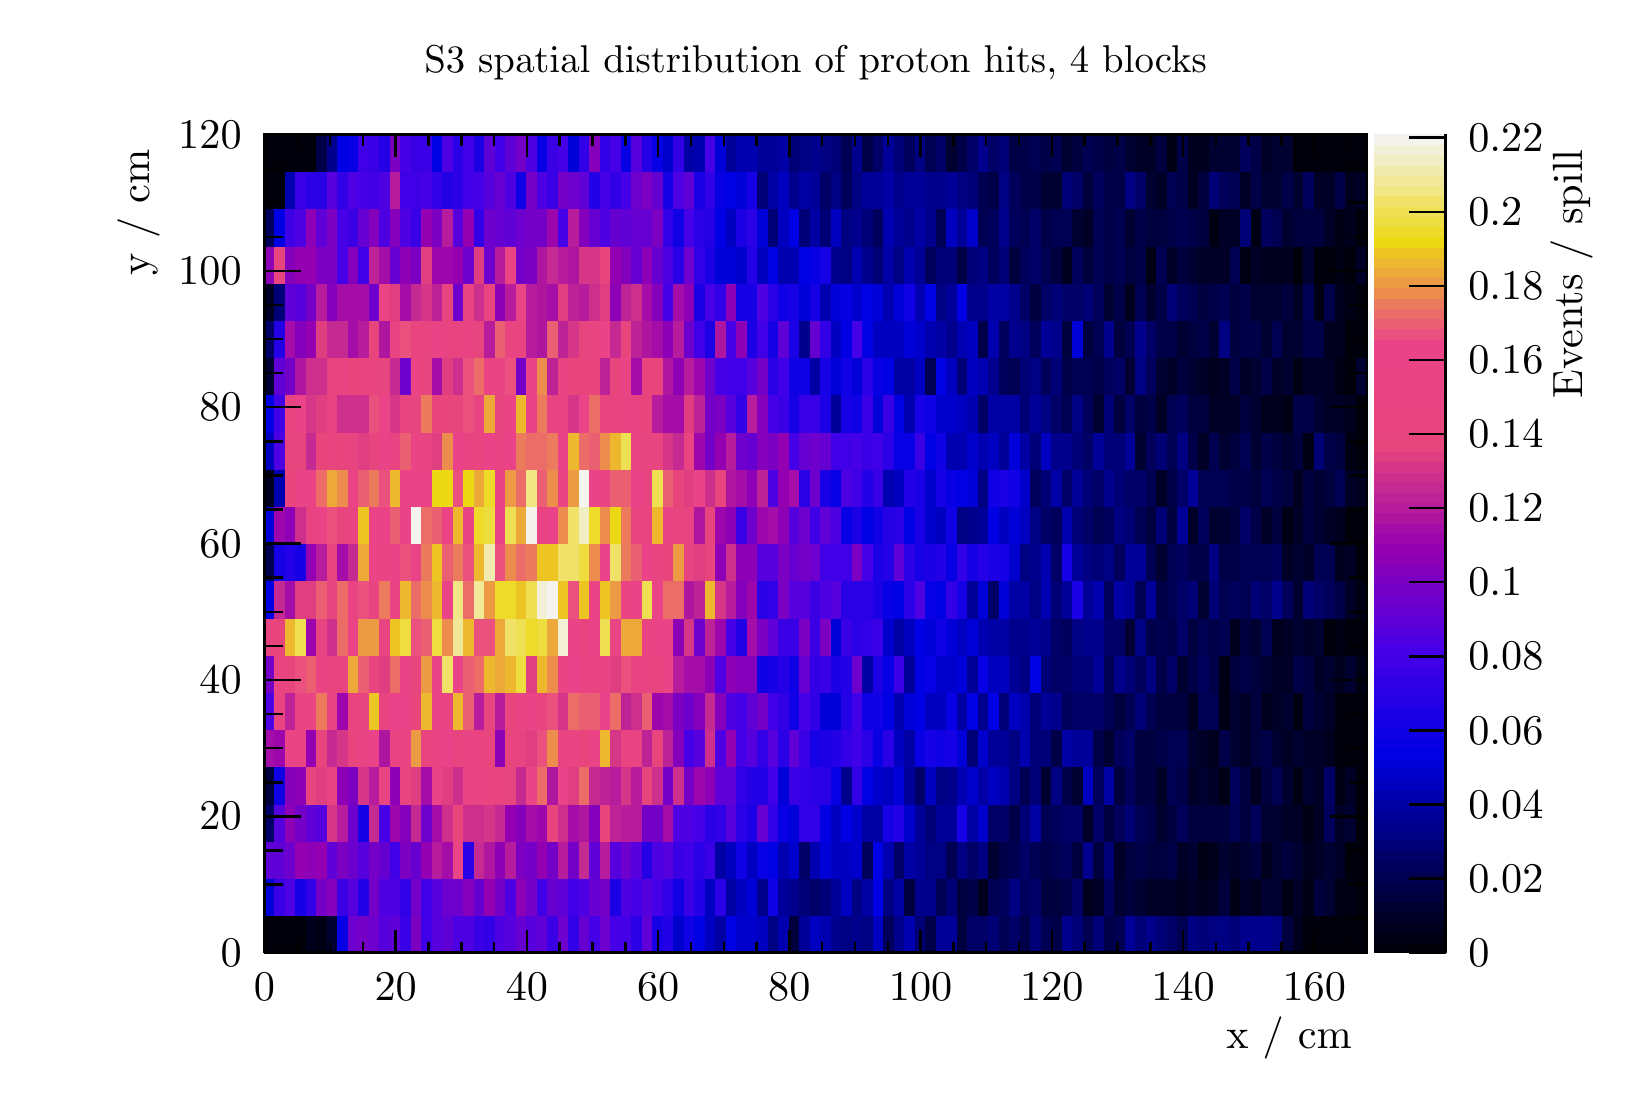
\begin{tikzpicture}
\pgfdeclareplotmark{cross} {
\pgfpathmoveto{\pgfpoint{-0.3\pgfplotmarksize}{\pgfplotmarksize}}
\pgfpathlineto{\pgfpoint{+0.3\pgfplotmarksize}{\pgfplotmarksize}}
\pgfpathlineto{\pgfpoint{+0.3\pgfplotmarksize}{0.3\pgfplotmarksize}}
\pgfpathlineto{\pgfpoint{+1\pgfplotmarksize}{0.3\pgfplotmarksize}}
\pgfpathlineto{\pgfpoint{+1\pgfplotmarksize}{-0.3\pgfplotmarksize}}
\pgfpathlineto{\pgfpoint{+0.3\pgfplotmarksize}{-0.3\pgfplotmarksize}}
\pgfpathlineto{\pgfpoint{+0.3\pgfplotmarksize}{-1.\pgfplotmarksize}}
\pgfpathlineto{\pgfpoint{-0.3\pgfplotmarksize}{-1.\pgfplotmarksize}}
\pgfpathlineto{\pgfpoint{-0.3\pgfplotmarksize}{-0.3\pgfplotmarksize}}
\pgfpathlineto{\pgfpoint{-1.\pgfplotmarksize}{-0.3\pgfplotmarksize}}
\pgfpathlineto{\pgfpoint{-1.\pgfplotmarksize}{0.3\pgfplotmarksize}}
\pgfpathlineto{\pgfpoint{-0.3\pgfplotmarksize}{0.3\pgfplotmarksize}}
\pgfpathclose
\pgfusepathqstroke
}
\pgfdeclareplotmark{cross*} {
\pgfpathmoveto{\pgfpoint{-0.3\pgfplotmarksize}{\pgfplotmarksize}}
\pgfpathlineto{\pgfpoint{+0.3\pgfplotmarksize}{\pgfplotmarksize}}
\pgfpathlineto{\pgfpoint{+0.3\pgfplotmarksize}{0.3\pgfplotmarksize}}
\pgfpathlineto{\pgfpoint{+1\pgfplotmarksize}{0.3\pgfplotmarksize}}
\pgfpathlineto{\pgfpoint{+1\pgfplotmarksize}{-0.3\pgfplotmarksize}}
\pgfpathlineto{\pgfpoint{+0.3\pgfplotmarksize}{-0.3\pgfplotmarksize}}
\pgfpathlineto{\pgfpoint{+0.3\pgfplotmarksize}{-1.\pgfplotmarksize}}
\pgfpathlineto{\pgfpoint{-0.3\pgfplotmarksize}{-1.\pgfplotmarksize}}
\pgfpathlineto{\pgfpoint{-0.3\pgfplotmarksize}{-0.3\pgfplotmarksize}}
\pgfpathlineto{\pgfpoint{-1.\pgfplotmarksize}{-0.3\pgfplotmarksize}}
\pgfpathlineto{\pgfpoint{-1.\pgfplotmarksize}{0.3\pgfplotmarksize}}
\pgfpathlineto{\pgfpoint{-0.3\pgfplotmarksize}{0.3\pgfplotmarksize}}
\pgfpathclose
\pgfusepathqfillstroke
}
\pgfdeclareplotmark{newstar} {
\pgfpathmoveto{\pgfqpoint{0pt}{\pgfplotmarksize}}
\pgfpathlineto{\pgfqpointpolar{44}{0.5\pgfplotmarksize}}
\pgfpathlineto{\pgfqpointpolar{18}{\pgfplotmarksize}}
\pgfpathlineto{\pgfqpointpolar{-20}{0.5\pgfplotmarksize}}
\pgfpathlineto{\pgfqpointpolar{-54}{\pgfplotmarksize}}
\pgfpathlineto{\pgfqpointpolar{-90}{0.5\pgfplotmarksize}}
\pgfpathlineto{\pgfqpointpolar{234}{\pgfplotmarksize}}
\pgfpathlineto{\pgfqpointpolar{198}{0.5\pgfplotmarksize}}
\pgfpathlineto{\pgfqpointpolar{162}{\pgfplotmarksize}}
\pgfpathlineto{\pgfqpointpolar{134}{0.5\pgfplotmarksize}}
\pgfpathclose
\pgfusepathqstroke
}
\pgfdeclareplotmark{newstar*} {
\pgfpathmoveto{\pgfqpoint{0pt}{\pgfplotmarksize}}
\pgfpathlineto{\pgfqpointpolar{44}{0.5\pgfplotmarksize}}
\pgfpathlineto{\pgfqpointpolar{18}{\pgfplotmarksize}}
\pgfpathlineto{\pgfqpointpolar{-20}{0.5\pgfplotmarksize}}
\pgfpathlineto{\pgfqpointpolar{-54}{\pgfplotmarksize}}
\pgfpathlineto{\pgfqpointpolar{-90}{0.5\pgfplotmarksize}}
\pgfpathlineto{\pgfqpointpolar{234}{\pgfplotmarksize}}
\pgfpathlineto{\pgfqpointpolar{198}{0.5\pgfplotmarksize}}
\pgfpathlineto{\pgfqpointpolar{162}{\pgfplotmarksize}}
\pgfpathlineto{\pgfqpointpolar{134}{0.5\pgfplotmarksize}}
\pgfpathclose
\pgfusepathqfillstroke
}
\definecolor{c}{rgb}{1,1,1};
\draw [color=c, fill=c] (0,0) rectangle (20,13.4957);
\draw [color=c, fill=c] (3,1.75444) rectangle (17,12.1461);
\definecolor{c}{rgb}{0,0,0};
\draw [c,line width=0.9] (3,1.75444) -- (3,12.1461) -- (17,12.1461) -- (17,1.75444) -- (3,1.75444);
\definecolor{c}{rgb}{1,1,1};
\draw [color=c, fill=c] (3,1.75444) rectangle (17,12.1461);
\definecolor{c}{rgb}{0,0,0};
\draw [c,line width=0.9] (3,1.75444) -- (3,12.1461) -- (17,12.1461) -- (17,1.75444) -- (3,1.75444);
\definecolor{c}{rgb}{0,0,0.0387097};
\draw [color=c, fill=c] (3,1.75444) rectangle (3.13333,2.22679);
\draw [color=c, fill=c] (3.13333,1.75444) rectangle (3.26667,2.22679);
\draw [color=c, fill=c] (3.26667,1.75444) rectangle (3.4,2.22679);
\draw [color=c, fill=c] (3.4,1.75444) rectangle (3.53333,2.22679);
\definecolor{c}{rgb}{0,0,0.116129};
\draw [color=c, fill=c] (3.53333,1.75444) rectangle (3.66667,2.22679);
\definecolor{c}{rgb}{0,0,0.0774194};
\draw [color=c, fill=c] (3.66667,1.75444) rectangle (3.8,2.22679);
\definecolor{c}{rgb}{0,0,0.193548};
\draw [color=c, fill=c] (3.8,1.75444) rectangle (3.93333,2.22679);
\definecolor{c}{rgb}{0.0257353,0,0.895221};
\draw [color=c, fill=c] (3.93333,1.75444) rectangle (4.06667,2.22679);
\definecolor{c}{rgb}{0.427451,0,0.8};
\draw [color=c, fill=c] (4.06667,1.75444) rectangle (4.2,2.22679);
\definecolor{c}{rgb}{0.456127,0,0.780147};
\draw [color=c, fill=c] (4.2,1.75444) rectangle (4.33333,2.22679);
\definecolor{c}{rgb}{0.427451,0,0.8};
\draw [color=c, fill=c] (4.33333,1.75444) rectangle (4.46667,2.22679);
\definecolor{c}{rgb}{0.331863,0,0.866176};
\draw [color=c, fill=c] (4.46667,1.75444) rectangle (4.6,2.22679);
\definecolor{c}{rgb}{0.370098,0,0.839706};
\draw [color=c, fill=c] (4.6,1.75444) rectangle (4.73333,2.22679);
\definecolor{c}{rgb}{0.223039,0,0.903676};
\draw [color=c, fill=c] (4.73333,1.75444) rectangle (4.86667,2.22679);
\definecolor{c}{rgb}{0.484804,0,0.760294};
\draw [color=c, fill=c] (4.86667,1.75444) rectangle (5,2.22679);
\definecolor{c}{rgb}{0.248775,0,0.904779};
\draw [color=c, fill=c] (5,1.75444) rectangle (5.13333,2.22679);
\definecolor{c}{rgb}{0.331863,0,0.866176};
\draw [color=c, fill=c] (5.13333,1.75444) rectangle (5.26667,2.22679);
\definecolor{c}{rgb}{0.370098,0,0.839706};
\draw [color=c, fill=c] (5.26667,1.75444) rectangle (5.4,2.22679);
\definecolor{c}{rgb}{0.303186,0,0.886029};
\draw [color=c, fill=c] (5.4,1.75444) rectangle (5.53333,2.22679);
\draw [color=c, fill=c] (5.53333,1.75444) rectangle (5.66667,2.22679);
\definecolor{c}{rgb}{0.223039,0,0.903676};
\draw [color=c, fill=c] (5.66667,1.75444) rectangle (5.8,2.22679);
\definecolor{c}{rgb}{0.197304,0,0.902574};
\draw [color=c, fill=c] (5.8,1.75444) rectangle (5.93333,2.22679);
\definecolor{c}{rgb}{0.303186,0,0.886029};
\draw [color=c, fill=c] (5.93333,1.75444) rectangle (6.06667,2.22679);
\definecolor{c}{rgb}{0.331863,0,0.866176};
\draw [color=c, fill=c] (6.06667,1.75444) rectangle (6.2,2.22679);
\definecolor{c}{rgb}{0.398775,0,0.819853};
\draw [color=c, fill=c] (6.2,1.75444) rectangle (6.33333,2.22679);
\definecolor{c}{rgb}{0.331863,0,0.866176};
\draw [color=c, fill=c] (6.33333,1.75444) rectangle (6.46667,2.22679);
\definecolor{c}{rgb}{0.370098,0,0.839706};
\draw [color=c, fill=c] (6.46667,1.75444) rectangle (6.6,2.22679);
\definecolor{c}{rgb}{0.223039,0,0.903676};
\draw [color=c, fill=c] (6.6,1.75444) rectangle (6.73333,2.22679);
\definecolor{c}{rgb}{0.427451,0,0.8};
\draw [color=c, fill=c] (6.73333,1.75444) rectangle (6.86667,2.22679);
\definecolor{c}{rgb}{0.197304,0,0.902574};
\draw [color=c, fill=c] (6.86667,1.75444) rectangle (7,2.22679);
\definecolor{c}{rgb}{0.398775,0,0.819853};
\draw [color=c, fill=c] (7,1.75444) rectangle (7.13333,2.22679);
\definecolor{c}{rgb}{0.27451,0,0.905882};
\draw [color=c, fill=c] (7.13333,1.75444) rectangle (7.26667,2.22679);
\definecolor{c}{rgb}{0.427451,0,0.8};
\draw [color=c, fill=c] (7.26667,1.75444) rectangle (7.4,2.22679);
\definecolor{c}{rgb}{0.27451,0,0.905882};
\draw [color=c, fill=c] (7.4,1.75444) rectangle (7.53333,2.22679);
\draw [color=c, fill=c] (7.53333,1.75444) rectangle (7.66667,2.22679);
\definecolor{c}{rgb}{0.16299,0,0.901103};
\draw [color=c, fill=c] (7.66667,1.75444) rectangle (7.8,2.22679);
\definecolor{c}{rgb}{0.370098,0,0.839706};
\draw [color=c, fill=c] (7.8,1.75444) rectangle (7.93333,2.22679);
\definecolor{c}{rgb}{0.0857843,0,0.897794};
\draw [color=c, fill=c] (7.93333,1.75444) rectangle (8.06667,2.22679);
\definecolor{c}{rgb}{0.137255,0,0.9};
\draw [color=c, fill=c] (8.06667,1.75444) rectangle (8.2,2.22679);
\definecolor{c}{rgb}{0,0,0.801471};
\draw [color=c, fill=c] (8.2,1.75444) rectangle (8.33333,2.22679);
\definecolor{c}{rgb}{0.060049,0,0.896691};
\draw [color=c, fill=c] (8.33333,1.75444) rectangle (8.46667,2.22679);
\definecolor{c}{rgb}{0,0,0.894118};
\draw [color=c, fill=c] (8.46667,1.75444) rectangle (8.6,2.22679);
\definecolor{c}{rgb}{0,0,0.755147};
\draw [color=c, fill=c] (8.6,1.75444) rectangle (8.73333,2.22679);
\definecolor{c}{rgb}{0,0,0.647059};
\draw [color=c, fill=c] (8.73333,1.75444) rectangle (8.86667,2.22679);
\definecolor{c}{rgb}{0,0,0.894118};
\draw [color=c, fill=c] (8.86667,1.75444) rectangle (9,2.22679);
\definecolor{c}{rgb}{0,0,0.801471};
\draw [color=c, fill=c] (9,1.75444) rectangle (9.13333,2.22679);
\draw [color=c, fill=c] (9.13333,1.75444) rectangle (9.26667,2.22679);
\definecolor{c}{rgb}{0,0,0.755147};
\draw [color=c, fill=c] (9.26667,1.75444) rectangle (9.4,2.22679);
\definecolor{c}{rgb}{0,0,0.508088};
\draw [color=c, fill=c] (9.4,1.75444) rectangle (9.53333,2.22679);
\definecolor{c}{rgb}{0,0,0.693382};
\draw [color=c, fill=c] (9.53333,1.75444) rectangle (9.66667,2.22679);
\definecolor{c}{rgb}{0,0,0.245161};
\draw [color=c, fill=c] (9.66667,1.75444) rectangle (9.8,2.22679);
\definecolor{c}{rgb}{0,0,0.600735};
\draw [color=c, fill=c] (9.8,1.75444) rectangle (9.93333,2.22679);
\definecolor{c}{rgb}{0,0,0.755147};
\draw [color=c, fill=c] (9.93333,1.75444) rectangle (10.0667,2.22679);
\definecolor{c}{rgb}{0,0,0.693382};
\draw [color=c, fill=c] (10.0667,1.75444) rectangle (10.2,2.22679);
\definecolor{c}{rgb}{0,0,0.554412};
\draw [color=c, fill=c] (10.2,1.75444) rectangle (10.3333,2.22679);
\definecolor{c}{rgb}{0,0,0.508088};
\draw [color=c, fill=c] (10.3333,1.75444) rectangle (10.4667,2.22679);
\definecolor{c}{rgb}{0,0,0.554412};
\draw [color=c, fill=c] (10.4667,1.75444) rectangle (10.6,2.22679);
\definecolor{c}{rgb}{0,0,0.508088};
\draw [color=c, fill=c] (10.6,1.75444) rectangle (10.7333,2.22679);
\definecolor{c}{rgb}{0,0,0.755147};
\draw [color=c, fill=c] (10.7333,1.75444) rectangle (10.8667,2.22679);
\definecolor{c}{rgb}{0,0,0.36129};
\draw [color=c, fill=c] (10.8667,1.75444) rectangle (11,2.22679);
\definecolor{c}{rgb}{0,0,0.554412};
\draw [color=c, fill=c] (11,1.75444) rectangle (11.1333,2.22679);
\definecolor{c}{rgb}{0,0,0.693382};
\draw [color=c, fill=c] (11.1333,1.75444) rectangle (11.2667,2.22679);
\definecolor{c}{rgb}{0,0,0.461765};
\draw [color=c, fill=c] (11.2667,1.75444) rectangle (11.4,2.22679);
\definecolor{c}{rgb}{0,0,0.283871};
\draw [color=c, fill=c] (11.4,1.75444) rectangle (11.5333,2.22679);
\definecolor{c}{rgb}{0,0,0.600735};
\draw [color=c, fill=c] (11.5333,1.75444) rectangle (11.6667,2.22679);
\draw [color=c, fill=c] (11.6667,1.75444) rectangle (11.8,2.22679);
\definecolor{c}{rgb}{0,0,0.245161};
\draw [color=c, fill=c] (11.8,1.75444) rectangle (11.9333,2.22679);
\definecolor{c}{rgb}{0,0,0.4};
\draw [color=c, fill=c] (11.9333,1.75444) rectangle (12.0667,2.22679);
\draw [color=c, fill=c] (12.0667,1.75444) rectangle (12.2,2.22679);
\definecolor{c}{rgb}{0,0,0.461765};
\draw [color=c, fill=c] (12.2,1.75444) rectangle (12.3333,2.22679);
\definecolor{c}{rgb}{0,0,0.322581};
\draw [color=c, fill=c] (12.3333,1.75444) rectangle (12.4667,2.22679);
\definecolor{c}{rgb}{0,0,0.4};
\draw [color=c, fill=c] (12.4667,1.75444) rectangle (12.6,2.22679);
\definecolor{c}{rgb}{0,0,0.283871};
\draw [color=c, fill=c] (12.6,1.75444) rectangle (12.7333,2.22679);
\definecolor{c}{rgb}{0,0,0.461765};
\draw [color=c, fill=c] (12.7333,1.75444) rectangle (12.8667,2.22679);
\definecolor{c}{rgb}{0,0,0.322581};
\draw [color=c, fill=c] (12.8667,1.75444) rectangle (13,2.22679);
\definecolor{c}{rgb}{0,0,0.283871};
\draw [color=c, fill=c] (13,1.75444) rectangle (13.1333,2.22679);
\definecolor{c}{rgb}{0,0,0.554412};
\draw [color=c, fill=c] (13.1333,1.75444) rectangle (13.2667,2.22679);
\definecolor{c}{rgb}{0,0,0.461765};
\draw [color=c, fill=c] (13.2667,1.75444) rectangle (13.4,2.22679);
\definecolor{c}{rgb}{0,0,0.322581};
\draw [color=c, fill=c] (13.4,1.75444) rectangle (13.5333,2.22679);
\definecolor{c}{rgb}{0,0,0.461765};
\draw [color=c, fill=c] (13.5333,1.75444) rectangle (13.6667,2.22679);
\definecolor{c}{rgb}{0,0,0.283871};
\draw [color=c, fill=c] (13.6667,1.75444) rectangle (13.8,2.22679);
\definecolor{c}{rgb}{0,0,0.322581};
\draw [color=c, fill=c] (13.8,1.75444) rectangle (13.9333,2.22679);
\definecolor{c}{rgb}{0,0,0.600735};
\draw [color=c, fill=c] (13.9333,1.75444) rectangle (14.0667,2.22679);
\definecolor{c}{rgb}{0,0,0.461765};
\draw [color=c, fill=c] (14.0667,1.75444) rectangle (14.2,2.22679);
\definecolor{c}{rgb}{0,0,0.554412};
\draw [color=c, fill=c] (14.2,1.75444) rectangle (14.3333,2.22679);
\definecolor{c}{rgb}{0,0,0.461765};
\draw [color=c, fill=c] (14.3333,1.75444) rectangle (14.4667,2.22679);
\definecolor{c}{rgb}{0,0,0.4};
\draw [color=c, fill=c] (14.4667,1.75444) rectangle (14.6,2.22679);
\definecolor{c}{rgb}{0,0,0.322581};
\draw [color=c, fill=c] (14.6,1.75444) rectangle (14.7333,2.22679);
\definecolor{c}{rgb}{0,0,0.508088};
\draw [color=c, fill=c] (14.7333,1.75444) rectangle (14.8667,2.22679);
\definecolor{c}{rgb}{0,0,0.461765};
\draw [color=c, fill=c] (14.8667,1.75444) rectangle (15,2.22679);
\definecolor{c}{rgb}{0,0,0.508088};
\draw [color=c, fill=c] (15,1.75444) rectangle (15.1333,2.22679);
\draw [color=c, fill=c] (15.1333,1.75444) rectangle (15.2667,2.22679);
\definecolor{c}{rgb}{0,0,0.461765};
\draw [color=c, fill=c] (15.2667,1.75444) rectangle (15.4,2.22679);
\definecolor{c}{rgb}{0,0,0.554412};
\draw [color=c, fill=c] (15.4,1.75444) rectangle (15.5333,2.22679);
\draw [color=c, fill=c] (15.5333,1.75444) rectangle (15.6667,2.22679);
\draw [color=c, fill=c] (15.6667,1.75444) rectangle (15.8,2.22679);
\definecolor{c}{rgb}{0,0,0.508088};
\draw [color=c, fill=c] (15.8,1.75444) rectangle (15.9333,2.22679);
\definecolor{c}{rgb}{0,0,0.245161};
\draw [color=c, fill=c] (15.9333,1.75444) rectangle (16.0667,2.22679);
\definecolor{c}{rgb}{0,0,0.116129};
\draw [color=c, fill=c] (16.0667,1.75444) rectangle (16.2,2.22679);
\definecolor{c}{rgb}{0,0,0.0387097};
\draw [color=c, fill=c] (16.2,1.75444) rectangle (16.3333,2.22679);
\draw [color=c, fill=c] (16.3333,1.75444) rectangle (16.4667,2.22679);
\draw [color=c, fill=c] (16.4667,1.75444) rectangle (16.6,2.22679);
\draw [color=c, fill=c] (16.6,1.75444) rectangle (16.7333,2.22679);
\draw [color=c, fill=c] (16.7333,1.75444) rectangle (16.8667,2.22679);
\draw [color=c, fill=c] (16.8667,1.75444) rectangle (17,2.22679);
\definecolor{c}{rgb}{0,0,0.847794};
\draw [color=c, fill=c] (3,2.22679) rectangle (3.13333,2.69914);
\definecolor{c}{rgb}{0.223039,0,0.903676};
\draw [color=c, fill=c] (3.13333,2.22679) rectangle (3.26667,2.69914);
\definecolor{c}{rgb}{0.303186,0,0.886029};
\draw [color=c, fill=c] (3.26667,2.22679) rectangle (3.4,2.69914);
\definecolor{c}{rgb}{0.0857843,0,0.897794};
\draw [color=c, fill=c] (3.4,2.22679) rectangle (3.53333,2.69914);
\definecolor{c}{rgb}{0.197304,0,0.902574};
\draw [color=c, fill=c] (3.53333,2.22679) rectangle (3.66667,2.69914);
\definecolor{c}{rgb}{0.456127,0,0.780147};
\draw [color=c, fill=c] (3.66667,2.22679) rectangle (3.8,2.69914);
\definecolor{c}{rgb}{0.523039,0,0.733824};
\draw [color=c, fill=c] (3.8,2.22679) rectangle (3.93333,2.69914);
\definecolor{c}{rgb}{0.223039,0,0.903676};
\draw [color=c, fill=c] (3.93333,2.22679) rectangle (4.06667,2.69914);
\definecolor{c}{rgb}{0.331863,0,0.866176};
\draw [color=c, fill=c] (4.06667,2.22679) rectangle (4.2,2.69914);
\definecolor{c}{rgb}{0.137255,0,0.9};
\draw [color=c, fill=c] (4.2,2.22679) rectangle (4.33333,2.69914);
\definecolor{c}{rgb}{0.456127,0,0.780147};
\draw [color=c, fill=c] (4.33333,2.22679) rectangle (4.46667,2.69914);
\definecolor{c}{rgb}{0.303186,0,0.886029};
\draw [color=c, fill=c] (4.46667,2.22679) rectangle (4.6,2.69914);
\draw [color=c, fill=c] (4.6,2.22679) rectangle (4.73333,2.69914);
\definecolor{c}{rgb}{0.197304,0,0.902574};
\draw [color=c, fill=c] (4.73333,2.22679) rectangle (4.86667,2.69914);
\definecolor{c}{rgb}{0.456127,0,0.780147};
\draw [color=c, fill=c] (4.86667,2.22679) rectangle (5,2.69914);
\definecolor{c}{rgb}{0.248775,0,0.904779};
\draw [color=c, fill=c] (5,2.22679) rectangle (5.13333,2.69914);
\definecolor{c}{rgb}{0.331863,0,0.866176};
\draw [color=c, fill=c] (5.13333,2.22679) rectangle (5.26667,2.69914);
\definecolor{c}{rgb}{0.427451,0,0.8};
\draw [color=c, fill=c] (5.26667,2.22679) rectangle (5.4,2.69914);
\draw [color=c, fill=c] (5.4,2.22679) rectangle (5.53333,2.69914);
\definecolor{c}{rgb}{0.523039,0,0.733824};
\draw [color=c, fill=c] (5.53333,2.22679) rectangle (5.66667,2.69914);
\definecolor{c}{rgb}{0.398775,0,0.819853};
\draw [color=c, fill=c] (5.66667,2.22679) rectangle (5.8,2.69914);
\definecolor{c}{rgb}{0.580392,0,0.694118};
\draw [color=c, fill=c] (5.8,2.22679) rectangle (5.93333,2.69914);
\definecolor{c}{rgb}{0.456127,0,0.780147};
\draw [color=c, fill=c] (5.93333,2.22679) rectangle (6.06667,2.69914);
\definecolor{c}{rgb}{0.303186,0,0.886029};
\draw [color=c, fill=c] (6.06667,2.22679) rectangle (6.2,2.69914);
\definecolor{c}{rgb}{0.551716,0,0.713971};
\draw [color=c, fill=c] (6.2,2.22679) rectangle (6.33333,2.69914);
\definecolor{c}{rgb}{0.456127,0,0.780147};
\draw [color=c, fill=c] (6.33333,2.22679) rectangle (6.46667,2.69914);
\definecolor{c}{rgb}{0.248775,0,0.904779};
\draw [color=c, fill=c] (6.46667,2.22679) rectangle (6.6,2.69914);
\definecolor{c}{rgb}{0.398775,0,0.819853};
\draw [color=c, fill=c] (6.6,2.22679) rectangle (6.73333,2.69914);
\definecolor{c}{rgb}{0.370098,0,0.839706};
\draw [color=c, fill=c] (6.73333,2.22679) rectangle (6.86667,2.69914);
\definecolor{c}{rgb}{0.248775,0,0.904779};
\draw [color=c, fill=c] (6.86667,2.22679) rectangle (7,2.69914);
\definecolor{c}{rgb}{0.303186,0,0.886029};
\draw [color=c, fill=c] (7,2.22679) rectangle (7.13333,2.69914);
\definecolor{c}{rgb}{0.398775,0,0.819853};
\draw [color=c, fill=c] (7.13333,2.22679) rectangle (7.26667,2.69914);
\definecolor{c}{rgb}{0.456127,0,0.780147};
\draw [color=c, fill=c] (7.26667,2.22679) rectangle (7.4,2.69914);
\definecolor{c}{rgb}{0.11152,0,0.898897};
\draw [color=c, fill=c] (7.4,2.22679) rectangle (7.53333,2.69914);
\definecolor{c}{rgb}{0.303186,0,0.886029};
\draw [color=c, fill=c] (7.53333,2.22679) rectangle (7.66667,2.69914);
\definecolor{c}{rgb}{0.27451,0,0.905882};
\draw [color=c, fill=c] (7.66667,2.22679) rectangle (7.8,2.69914);
\definecolor{c}{rgb}{0.331863,0,0.866176};
\draw [color=c, fill=c] (7.8,2.22679) rectangle (7.93333,2.69914);
\definecolor{c}{rgb}{0.27451,0,0.905882};
\draw [color=c, fill=c] (7.93333,2.22679) rectangle (8.06667,2.69914);
\definecolor{c}{rgb}{0.197304,0,0.902574};
\draw [color=c, fill=c] (8.06667,2.22679) rectangle (8.2,2.69914);
\definecolor{c}{rgb}{0.060049,0,0.896691};
\draw [color=c, fill=c] (8.2,2.22679) rectangle (8.33333,2.69914);
\definecolor{c}{rgb}{0.223039,0,0.903676};
\draw [color=c, fill=c] (8.33333,2.22679) rectangle (8.46667,2.69914);
\definecolor{c}{rgb}{0.137255,0,0.9};
\draw [color=c, fill=c] (8.46667,2.22679) rectangle (8.6,2.69914);
\definecolor{c}{rgb}{0,0,0.755147};
\draw [color=c, fill=c] (8.6,2.22679) rectangle (8.73333,2.69914);
\definecolor{c}{rgb}{0.16299,0,0.901103};
\draw [color=c, fill=c] (8.73333,2.22679) rectangle (8.86667,2.69914);
\definecolor{c}{rgb}{0,0,0.647059};
\draw [color=c, fill=c] (8.86667,2.22679) rectangle (9,2.69914);
\definecolor{c}{rgb}{0,0,0.755147};
\draw [color=c, fill=c] (9,2.22679) rectangle (9.13333,2.69914);
\definecolor{c}{rgb}{0,0,0.847794};
\draw [color=c, fill=c] (9.13333,2.22679) rectangle (9.26667,2.69914);
\definecolor{c}{rgb}{0,0,0.554412};
\draw [color=c, fill=c] (9.26667,2.22679) rectangle (9.4,2.69914);
\definecolor{c}{rgb}{0.060049,0,0.896691};
\draw [color=c, fill=c] (9.4,2.22679) rectangle (9.53333,2.69914);
\definecolor{c}{rgb}{0,0,0.600735};
\draw [color=c, fill=c] (9.53333,2.22679) rectangle (9.66667,2.69914);
\definecolor{c}{rgb}{0,0,0.554412};
\draw [color=c, fill=c] (9.66667,2.22679) rectangle (9.8,2.69914);
\definecolor{c}{rgb}{0,0,0.461765};
\draw [color=c, fill=c] (9.8,2.22679) rectangle (9.93333,2.69914);
\definecolor{c}{rgb}{0,0,0.4};
\draw [color=c, fill=c] (9.93333,2.22679) rectangle (10.0667,2.69914);
\definecolor{c}{rgb}{0,0,0.461765};
\draw [color=c, fill=c] (10.0667,2.22679) rectangle (10.2,2.69914);
\definecolor{c}{rgb}{0,0,0.600735};
\draw [color=c, fill=c] (10.2,2.22679) rectangle (10.3333,2.69914);
\definecolor{c}{rgb}{0,0,0.755147};
\draw [color=c, fill=c] (10.3333,2.22679) rectangle (10.4667,2.69914);
\definecolor{c}{rgb}{0,0,0.508088};
\draw [color=c, fill=c] (10.4667,2.22679) rectangle (10.6,2.69914);
\definecolor{c}{rgb}{0,0,0.647059};
\draw [color=c, fill=c] (10.6,2.22679) rectangle (10.7333,2.69914);
\definecolor{c}{rgb}{0,0,0.894118};
\draw [color=c, fill=c] (10.7333,2.22679) rectangle (10.8667,2.69914);
\definecolor{c}{rgb}{0,0,0.508088};
\draw [color=c, fill=c] (10.8667,2.22679) rectangle (11,2.69914);
\definecolor{c}{rgb}{0,0,0.647059};
\draw [color=c, fill=c] (11,2.22679) rectangle (11.1333,2.69914);
\definecolor{c}{rgb}{0,0,0.245161};
\draw [color=c, fill=c] (11.1333,2.22679) rectangle (11.2667,2.69914);
\definecolor{c}{rgb}{0,0,0.554412};
\draw [color=c, fill=c] (11.2667,2.22679) rectangle (11.4,2.69914);
\draw [color=c, fill=c] (11.4,2.22679) rectangle (11.5333,2.69914);
\definecolor{c}{rgb}{0,0,0.322581};
\draw [color=c, fill=c] (11.5333,2.22679) rectangle (11.6667,2.69914);
\definecolor{c}{rgb}{0,0,0.461765};
\draw [color=c, fill=c] (11.6667,2.22679) rectangle (11.8,2.69914);
\definecolor{c}{rgb}{0,0,0.245161};
\draw [color=c, fill=c] (11.8,2.22679) rectangle (11.9333,2.69914);
\definecolor{c}{rgb}{0,0,0.283871};
\draw [color=c, fill=c] (11.9333,2.22679) rectangle (12.0667,2.69914);
\definecolor{c}{rgb}{0,0,0.116129};
\draw [color=c, fill=c] (12.0667,2.22679) rectangle (12.2,2.69914);
\definecolor{c}{rgb}{0,0,0.322581};
\draw [color=c, fill=c] (12.2,2.22679) rectangle (12.3333,2.69914);
\definecolor{c}{rgb}{0,0,0.36129};
\draw [color=c, fill=c] (12.3333,2.22679) rectangle (12.4667,2.69914);
\definecolor{c}{rgb}{0,0,0.508088};
\draw [color=c, fill=c] (12.4667,2.22679) rectangle (12.6,2.69914);
\definecolor{c}{rgb}{0,0,0.36129};
\draw [color=c, fill=c] (12.6,2.22679) rectangle (12.7333,2.69914);
\definecolor{c}{rgb}{0,0,0.4};
\draw [color=c, fill=c] (12.7333,2.22679) rectangle (12.8667,2.69914);
\definecolor{c}{rgb}{0,0,0.245161};
\draw [color=c, fill=c] (12.8667,2.22679) rectangle (13,2.69914);
\draw [color=c, fill=c] (13,2.22679) rectangle (13.1333,2.69914);
\definecolor{c}{rgb}{0,0,0.283871};
\draw [color=c, fill=c] (13.1333,2.22679) rectangle (13.2667,2.69914);
\definecolor{c}{rgb}{0,0,0.4};
\draw [color=c, fill=c] (13.2667,2.22679) rectangle (13.4,2.69914);
\definecolor{c}{rgb}{0,0,0.116129};
\draw [color=c, fill=c] (13.4,2.22679) rectangle (13.5333,2.69914);
\definecolor{c}{rgb}{0,0,0.154839};
\draw [color=c, fill=c] (13.5333,2.22679) rectangle (13.6667,2.69914);
\definecolor{c}{rgb}{0,0,0.36129};
\draw [color=c, fill=c] (13.6667,2.22679) rectangle (13.8,2.69914);
\definecolor{c}{rgb}{0,0,0.193548};
\draw [color=c, fill=c] (13.8,2.22679) rectangle (13.9333,2.69914);
\definecolor{c}{rgb}{0,0,0.245161};
\draw [color=c, fill=c] (13.9333,2.22679) rectangle (14.0667,2.69914);
\definecolor{c}{rgb}{0,0,0.193548};
\draw [color=c, fill=c] (14.0667,2.22679) rectangle (14.2,2.69914);
\definecolor{c}{rgb}{0,0,0.154839};
\draw [color=c, fill=c] (14.2,2.22679) rectangle (14.3333,2.69914);
\draw [color=c, fill=c] (14.3333,2.22679) rectangle (14.4667,2.69914);
\draw [color=c, fill=c] (14.4667,2.22679) rectangle (14.6,2.69914);
\definecolor{c}{rgb}{0,0,0.116129};
\draw [color=c, fill=c] (14.6,2.22679) rectangle (14.7333,2.69914);
\definecolor{c}{rgb}{0,0,0.154839};
\draw [color=c, fill=c] (14.7333,2.22679) rectangle (14.8667,2.69914);
\definecolor{c}{rgb}{0,0,0.116129};
\draw [color=c, fill=c] (14.8667,2.22679) rectangle (15,2.69914);
\definecolor{c}{rgb}{0,0,0.154839};
\draw [color=c, fill=c] (15,2.22679) rectangle (15.1333,2.69914);
\definecolor{c}{rgb}{0,0,0.245161};
\draw [color=c, fill=c] (15.1333,2.22679) rectangle (15.2667,2.69914);
\definecolor{c}{rgb}{0,0,0.0774194};
\draw [color=c, fill=c] (15.2667,2.22679) rectangle (15.4,2.69914);
\definecolor{c}{rgb}{0,0,0.154839};
\draw [color=c, fill=c] (15.4,2.22679) rectangle (15.5333,2.69914);
\definecolor{c}{rgb}{0,0,0.116129};
\draw [color=c, fill=c] (15.5333,2.22679) rectangle (15.6667,2.69914);
\definecolor{c}{rgb}{0,0,0.193548};
\draw [color=c, fill=c] (15.6667,2.22679) rectangle (15.8,2.69914);
\draw [color=c, fill=c] (15.8,2.22679) rectangle (15.9333,2.69914);
\definecolor{c}{rgb}{0,0,0.0774194};
\draw [color=c, fill=c] (15.9333,2.22679) rectangle (16.0667,2.69914);
\definecolor{c}{rgb}{0,0,0.154839};
\draw [color=c, fill=c] (16.0667,2.22679) rectangle (16.2,2.69914);
\definecolor{c}{rgb}{0,0,0.0774194};
\draw [color=c, fill=c] (16.2,2.22679) rectangle (16.3333,2.69914);
\definecolor{c}{rgb}{0,0,0.245161};
\draw [color=c, fill=c] (16.3333,2.22679) rectangle (16.4667,2.69914);
\definecolor{c}{rgb}{0,0,0.193548};
\draw [color=c, fill=c] (16.4667,2.22679) rectangle (16.6,2.69914);
\definecolor{c}{rgb}{0,0,0.0774194};
\draw [color=c, fill=c] (16.6,2.22679) rectangle (16.7333,2.69914);
\draw [color=c, fill=c] (16.7333,2.22679) rectangle (16.8667,2.69914);
\definecolor{c}{rgb}{0,0,0.0387097};
\draw [color=c, fill=c] (16.8667,2.22679) rectangle (17,2.69914);
\definecolor{c}{rgb}{0.370098,0,0.839706};
\draw [color=c, fill=c] (3,2.69914) rectangle (3.13333,3.17149);
\draw [color=c, fill=c] (3.13333,2.69914) rectangle (3.26667,3.17149);
\definecolor{c}{rgb}{0.427451,0,0.8};
\draw [color=c, fill=c] (3.26667,2.69914) rectangle (3.4,3.17149);
\definecolor{c}{rgb}{0.580392,0,0.694118};
\draw [color=c, fill=c] (3.4,2.69914) rectangle (3.53333,3.17149);
\definecolor{c}{rgb}{0.551716,0,0.713971};
\draw [color=c, fill=c] (3.53333,2.69914) rectangle (3.66667,3.17149);
\definecolor{c}{rgb}{0.580392,0,0.694118};
\draw [color=c, fill=c] (3.66667,2.69914) rectangle (3.8,3.17149);
\definecolor{c}{rgb}{0.370098,0,0.839706};
\draw [color=c, fill=c] (3.8,2.69914) rectangle (3.93333,3.17149);
\definecolor{c}{rgb}{0.484804,0,0.760294};
\draw [color=c, fill=c] (3.93333,2.69914) rectangle (4.06667,3.17149);
\definecolor{c}{rgb}{0.427451,0,0.8};
\draw [color=c, fill=c] (4.06667,2.69914) rectangle (4.2,3.17149);
\definecolor{c}{rgb}{0.331863,0,0.866176};
\draw [color=c, fill=c] (4.2,2.69914) rectangle (4.33333,3.17149);
\definecolor{c}{rgb}{0.456127,0,0.780147};
\draw [color=c, fill=c] (4.33333,2.69914) rectangle (4.46667,3.17149);
\definecolor{c}{rgb}{0.398775,0,0.819853};
\draw [color=c, fill=c] (4.46667,2.69914) rectangle (4.6,3.17149);
\definecolor{c}{rgb}{0.248775,0,0.904779};
\draw [color=c, fill=c] (4.6,2.69914) rectangle (4.73333,3.17149);
\definecolor{c}{rgb}{0.484804,0,0.760294};
\draw [color=c, fill=c] (4.73333,2.69914) rectangle (4.86667,3.17149);
\definecolor{c}{rgb}{0.398775,0,0.819853};
\draw [color=c, fill=c] (4.86667,2.69914) rectangle (5,3.17149);
\definecolor{c}{rgb}{0.580392,0,0.694118};
\draw [color=c, fill=c] (5,2.69914) rectangle (5.13333,3.17149);
\definecolor{c}{rgb}{0.712623,0.109926,0.609681};
\draw [color=c, fill=c] (5.13333,2.69914) rectangle (5.26667,3.17149);
\definecolor{c}{rgb}{0.641422,0.0507353,0.655147};
\draw [color=c, fill=c] (5.26667,2.69914) rectangle (5.4,3.17149);
\definecolor{c}{rgb}{0.915196,0.265931,0.516544};
\draw [color=c, fill=c] (5.4,2.69914) rectangle (5.53333,3.17149);
\definecolor{c}{rgb}{0.16299,0,0.901103};
\draw [color=c, fill=c] (5.53333,2.69914) rectangle (5.66667,3.17149);
\definecolor{c}{rgb}{0.773652,0.160662,0.570711};
\draw [color=c, fill=c] (5.66667,2.69914) rectangle (5.8,3.17149);
\definecolor{c}{rgb}{0.682108,0.0845588,0.629167};
\draw [color=c, fill=c] (5.8,2.69914) rectangle (5.93333,3.17149);
\definecolor{c}{rgb}{0.551716,0,0.713971};
\draw [color=c, fill=c] (5.93333,2.69914) rectangle (6.06667,3.17149);
\definecolor{c}{rgb}{0.712623,0.109926,0.609681};
\draw [color=c, fill=c] (6.06667,2.69914) rectangle (6.2,3.17149);
\definecolor{c}{rgb}{0.484804,0,0.760294};
\draw [color=c, fill=c] (6.2,2.69914) rectangle (6.33333,3.17149);
\definecolor{c}{rgb}{0.456127,0,0.780147};
\draw [color=c, fill=c] (6.33333,2.69914) rectangle (6.46667,3.17149);
\definecolor{c}{rgb}{0.580392,0,0.694118};
\draw [color=c, fill=c] (6.46667,2.69914) rectangle (6.6,3.17149);
\definecolor{c}{rgb}{0.456127,0,0.780147};
\draw [color=c, fill=c] (6.6,2.69914) rectangle (6.73333,3.17149);
\definecolor{c}{rgb}{0.712623,0.109926,0.609681};
\draw [color=c, fill=c] (6.73333,2.69914) rectangle (6.86667,3.17149);
\definecolor{c}{rgb}{0.456127,0,0.780147};
\draw [color=c, fill=c] (6.86667,2.69914) rectangle (7,3.17149);
\definecolor{c}{rgb}{0.773652,0.160662,0.570711};
\draw [color=c, fill=c] (7,2.69914) rectangle (7.13333,3.17149);
\definecolor{c}{rgb}{0.370098,0,0.839706};
\draw [color=c, fill=c] (7.13333,2.69914) rectangle (7.26667,3.17149);
\definecolor{c}{rgb}{0.712623,0.109926,0.609681};
\draw [color=c, fill=c] (7.26667,2.69914) rectangle (7.4,3.17149);
\definecolor{c}{rgb}{0.331863,0,0.866176};
\draw [color=c, fill=c] (7.4,2.69914) rectangle (7.53333,3.17149);
\definecolor{c}{rgb}{0.427451,0,0.8};
\draw [color=c, fill=c] (7.53333,2.69914) rectangle (7.66667,3.17149);
\definecolor{c}{rgb}{0.331863,0,0.866176};
\draw [color=c, fill=c] (7.66667,2.69914) rectangle (7.8,3.17149);
\definecolor{c}{rgb}{0.137255,0,0.9};
\draw [color=c, fill=c] (7.8,2.69914) rectangle (7.93333,3.17149);
\definecolor{c}{rgb}{0.303186,0,0.886029};
\draw [color=c, fill=c] (7.93333,2.69914) rectangle (8.06667,3.17149);
\definecolor{c}{rgb}{0.331863,0,0.866176};
\draw [color=c, fill=c] (8.06667,2.69914) rectangle (8.2,3.17149);
\definecolor{c}{rgb}{0.223039,0,0.903676};
\draw [color=c, fill=c] (8.2,2.69914) rectangle (8.33333,3.17149);
\definecolor{c}{rgb}{0.248775,0,0.904779};
\draw [color=c, fill=c] (8.33333,2.69914) rectangle (8.46667,3.17149);
\definecolor{c}{rgb}{0.16299,0,0.901103};
\draw [color=c, fill=c] (8.46667,2.69914) rectangle (8.6,3.17149);
\definecolor{c}{rgb}{0.223039,0,0.903676};
\draw [color=c, fill=c] (8.6,2.69914) rectangle (8.73333,3.17149);
\definecolor{c}{rgb}{0,0,0.647059};
\draw [color=c, fill=c] (8.73333,2.69914) rectangle (8.86667,3.17149);
\definecolor{c}{rgb}{0,0,0.755147};
\draw [color=c, fill=c] (8.86667,2.69914) rectangle (9,3.17149);
\definecolor{c}{rgb}{0.060049,0,0.896691};
\draw [color=c, fill=c] (9,2.69914) rectangle (9.13333,3.17149);
\definecolor{c}{rgb}{0,0,0.755147};
\draw [color=c, fill=c] (9.13333,2.69914) rectangle (9.26667,3.17149);
\definecolor{c}{rgb}{0.0257353,0,0.895221};
\draw [color=c, fill=c] (9.26667,2.69914) rectangle (9.4,3.17149);
\definecolor{c}{rgb}{0,0,0.894118};
\draw [color=c, fill=c] (9.4,2.69914) rectangle (9.53333,3.17149);
\definecolor{c}{rgb}{0,0,0.693382};
\draw [color=c, fill=c] (9.53333,2.69914) rectangle (9.66667,3.17149);
\definecolor{c}{rgb}{0,0,0.801471};
\draw [color=c, fill=c] (9.66667,2.69914) rectangle (9.8,3.17149);
\definecolor{c}{rgb}{0,0,0.4};
\draw [color=c, fill=c] (9.8,2.69914) rectangle (9.93333,3.17149);
\definecolor{c}{rgb}{0,0,0.693382};
\draw [color=c, fill=c] (9.93333,2.69914) rectangle (10.0667,3.17149);
\definecolor{c}{rgb}{0,0,0.847794};
\draw [color=c, fill=c] (10.0667,2.69914) rectangle (10.2,3.17149);
\definecolor{c}{rgb}{0,0,0.755147};
\draw [color=c, fill=c] (10.2,2.69914) rectangle (10.3333,3.17149);
\draw [color=c, fill=c] (10.3333,2.69914) rectangle (10.4667,3.17149);
\definecolor{c}{rgb}{0,0,0.801471};
\draw [color=c, fill=c] (10.4667,2.69914) rectangle (10.6,3.17149);
\definecolor{c}{rgb}{0,0,0.36129};
\draw [color=c, fill=c] (10.6,2.69914) rectangle (10.7333,3.17149);
\definecolor{c}{rgb}{0,0,0.894118};
\draw [color=c, fill=c] (10.7333,2.69914) rectangle (10.8667,3.17149);
\definecolor{c}{rgb}{0,0,0.693382};
\draw [color=c, fill=c] (10.8667,2.69914) rectangle (11,3.17149);
\definecolor{c}{rgb}{0,0,0.4};
\draw [color=c, fill=c] (11,2.69914) rectangle (11.1333,3.17149);
\definecolor{c}{rgb}{0,0,0.647059};
\draw [color=c, fill=c] (11.1333,2.69914) rectangle (11.2667,3.17149);
\definecolor{c}{rgb}{0,0,0.600735};
\draw [color=c, fill=c] (11.2667,2.69914) rectangle (11.4,3.17149);
\definecolor{c}{rgb}{0,0,0.508088};
\draw [color=c, fill=c] (11.4,2.69914) rectangle (11.5333,3.17149);
\draw [color=c, fill=c] (11.5333,2.69914) rectangle (11.6667,3.17149);
\definecolor{c}{rgb}{0,0,0.322581};
\draw [color=c, fill=c] (11.6667,2.69914) rectangle (11.8,3.17149);
\definecolor{c}{rgb}{0,0,0.508088};
\draw [color=c, fill=c] (11.8,2.69914) rectangle (11.9333,3.17149);
\definecolor{c}{rgb}{0,0,0.4};
\draw [color=c, fill=c] (11.9333,2.69914) rectangle (12.0667,3.17149);
\definecolor{c}{rgb}{0,0,0.508088};
\draw [color=c, fill=c] (12.0667,2.69914) rectangle (12.2,3.17149);
\definecolor{c}{rgb}{0,0,0.193548};
\draw [color=c, fill=c] (12.2,2.69914) rectangle (12.3333,3.17149);
\definecolor{c}{rgb}{0,0,0.283871};
\draw [color=c, fill=c] (12.3333,2.69914) rectangle (12.4667,3.17149);
\definecolor{c}{rgb}{0,0,0.322581};
\draw [color=c, fill=c] (12.4667,2.69914) rectangle (12.6,3.17149);
\definecolor{c}{rgb}{0,0,0.4};
\draw [color=c, fill=c] (12.6,2.69914) rectangle (12.7333,3.17149);
\definecolor{c}{rgb}{0,0,0.322581};
\draw [color=c, fill=c] (12.7333,2.69914) rectangle (12.8667,3.17149);
\definecolor{c}{rgb}{0,0,0.283871};
\draw [color=c, fill=c] (12.8667,2.69914) rectangle (13,3.17149);
\definecolor{c}{rgb}{0,0,0.322581};
\draw [color=c, fill=c] (13,2.69914) rectangle (13.1333,3.17149);
\definecolor{c}{rgb}{0,0,0.36129};
\draw [color=c, fill=c] (13.1333,2.69914) rectangle (13.2667,3.17149);
\definecolor{c}{rgb}{0,0,0.245161};
\draw [color=c, fill=c] (13.2667,2.69914) rectangle (13.4,3.17149);
\definecolor{c}{rgb}{0,0,0.554412};
\draw [color=c, fill=c] (13.4,2.69914) rectangle (13.5333,3.17149);
\definecolor{c}{rgb}{0,0,0.245161};
\draw [color=c, fill=c] (13.5333,2.69914) rectangle (13.6667,3.17149);
\definecolor{c}{rgb}{0,0,0.461765};
\draw [color=c, fill=c] (13.6667,2.69914) rectangle (13.8,3.17149);
\definecolor{c}{rgb}{0,0,0.154839};
\draw [color=c, fill=c] (13.8,2.69914) rectangle (13.9333,3.17149);
\definecolor{c}{rgb}{0,0,0.245161};
\draw [color=c, fill=c] (13.9333,2.69914) rectangle (14.0667,3.17149);
\definecolor{c}{rgb}{0,0,0.283871};
\draw [color=c, fill=c] (14.0667,2.69914) rectangle (14.2,3.17149);
\definecolor{c}{rgb}{0,0,0.245161};
\draw [color=c, fill=c] (14.2,2.69914) rectangle (14.3333,3.17149);
\draw [color=c, fill=c] (14.3333,2.69914) rectangle (14.4667,3.17149);
\definecolor{c}{rgb}{0,0,0.283871};
\draw [color=c, fill=c] (14.4667,2.69914) rectangle (14.6,3.17149);
\definecolor{c}{rgb}{0,0,0.154839};
\draw [color=c, fill=c] (14.6,2.69914) rectangle (14.7333,3.17149);
\definecolor{c}{rgb}{0,0,0.193548};
\draw [color=c, fill=c] (14.7333,2.69914) rectangle (14.8667,3.17149);
\definecolor{c}{rgb}{0,0,0.0774194};
\draw [color=c, fill=c] (14.8667,2.69914) rectangle (15,3.17149);
\definecolor{c}{rgb}{0,0,0.116129};
\draw [color=c, fill=c] (15,2.69914) rectangle (15.1333,3.17149);
\definecolor{c}{rgb}{0,0,0.193548};
\draw [color=c, fill=c] (15.1333,2.69914) rectangle (15.2667,3.17149);
\definecolor{c}{rgb}{0,0,0.154839};
\draw [color=c, fill=c] (15.2667,2.69914) rectangle (15.4,3.17149);
\definecolor{c}{rgb}{0,0,0.193548};
\draw [color=c, fill=c] (15.4,2.69914) rectangle (15.5333,3.17149);
\definecolor{c}{rgb}{0,0,0.245161};
\draw [color=c, fill=c] (15.5333,2.69914) rectangle (15.6667,3.17149);
\definecolor{c}{rgb}{0,0,0.116129};
\draw [color=c, fill=c] (15.6667,2.69914) rectangle (15.8,3.17149);
\definecolor{c}{rgb}{0,0,0.193548};
\draw [color=c, fill=c] (15.8,2.69914) rectangle (15.9333,3.17149);
\definecolor{c}{rgb}{0,0,0.245161};
\draw [color=c, fill=c] (15.9333,2.69914) rectangle (16.0667,3.17149);
\definecolor{c}{rgb}{0,0,0.193548};
\draw [color=c, fill=c] (16.0667,2.69914) rectangle (16.2,3.17149);
\definecolor{c}{rgb}{0,0,0.116129};
\draw [color=c, fill=c] (16.2,2.69914) rectangle (16.3333,3.17149);
\definecolor{c}{rgb}{0,0,0.154839};
\draw [color=c, fill=c] (16.3333,2.69914) rectangle (16.4667,3.17149);
\definecolor{c}{rgb}{0,0,0.193548};
\draw [color=c, fill=c] (16.4667,2.69914) rectangle (16.6,3.17149);
\definecolor{c}{rgb}{0,0,0.154839};
\draw [color=c, fill=c] (16.6,2.69914) rectangle (16.7333,3.17149);
\definecolor{c}{rgb}{0,0,0.0387097};
\draw [color=c, fill=c] (16.7333,2.69914) rectangle (16.8667,3.17149);
\draw [color=c, fill=c] (16.8667,2.69914) rectangle (17,3.17149);
\definecolor{c}{rgb}{0,0,0.4};
\draw [color=c, fill=c] (3,3.17149) rectangle (3.13333,3.64384);
\definecolor{c}{rgb}{0.331863,0,0.866176};
\draw [color=c, fill=c] (3.13333,3.17149) rectangle (3.26667,3.64384);
\definecolor{c}{rgb}{0.551716,0,0.713971};
\draw [color=c, fill=c] (3.26667,3.17149) rectangle (3.4,3.64384);
\definecolor{c}{rgb}{0.456127,0,0.780147};
\draw [color=c, fill=c] (3.4,3.17149) rectangle (3.53333,3.64384);
\definecolor{c}{rgb}{0.370098,0,0.839706};
\draw [color=c, fill=c] (3.53333,3.17149) rectangle (3.66667,3.64384);
\definecolor{c}{rgb}{0.331863,0,0.866176};
\draw [color=c, fill=c] (3.66667,3.17149) rectangle (3.8,3.64384);
\definecolor{c}{rgb}{0.834681,0.211397,0.53174};
\draw [color=c, fill=c] (3.8,3.17149) rectangle (3.93333,3.64384);
\definecolor{c}{rgb}{0.712623,0.109926,0.609681};
\draw [color=c, fill=c] (3.93333,3.17149) rectangle (4.06667,3.64384);
\definecolor{c}{rgb}{0.427451,0,0.8};
\draw [color=c, fill=c] (4.06667,3.17149) rectangle (4.2,3.64384);
\definecolor{c}{rgb}{0.0857843,0,0.897794};
\draw [color=c, fill=c] (4.2,3.17149) rectangle (4.33333,3.64384);
\definecolor{c}{rgb}{0.773652,0.160662,0.570711};
\draw [color=c, fill=c] (4.33333,3.17149) rectangle (4.46667,3.64384);
\definecolor{c}{rgb}{0.27451,0,0.905882};
\draw [color=c, fill=c] (4.46667,3.17149) rectangle (4.6,3.64384);
\definecolor{c}{rgb}{0.610907,0.0253676,0.674632};
\draw [color=c, fill=c] (4.6,3.17149) rectangle (4.73333,3.64384);
\definecolor{c}{rgb}{0.523039,0,0.733824};
\draw [color=c, fill=c] (4.73333,3.17149) rectangle (4.86667,3.64384);
\definecolor{c}{rgb}{0.773652,0.160662,0.570711};
\draw [color=c, fill=c] (4.86667,3.17149) rectangle (5,3.64384);
\definecolor{c}{rgb}{0.427451,0,0.8};
\draw [color=c, fill=c] (5,3.17149) rectangle (5.13333,3.64384);
\definecolor{c}{rgb}{0.641422,0.0507353,0.655147};
\draw [color=c, fill=c] (5.13333,3.17149) rectangle (5.26667,3.64384);
\definecolor{c}{rgb}{0.804167,0.186029,0.551225};
\draw [color=c, fill=c] (5.26667,3.17149) rectangle (5.4,3.64384);
\definecolor{c}{rgb}{0.905882,0.270588,0.486275};
\draw [color=c, fill=c] (5.4,3.17149) rectangle (5.53333,3.64384);
\definecolor{c}{rgb}{0.804167,0.186029,0.551225};
\draw [color=c, fill=c] (5.53333,3.17149) rectangle (5.66667,3.64384);
\draw [color=c, fill=c] (5.66667,3.17149) rectangle (5.8,3.64384);
\definecolor{c}{rgb}{0.834681,0.211397,0.53174};
\draw [color=c, fill=c] (5.8,3.17149) rectangle (5.93333,3.64384);
\definecolor{c}{rgb}{0.773652,0.160662,0.570711};
\draw [color=c, fill=c] (5.93333,3.17149) rectangle (6.06667,3.64384);
\definecolor{c}{rgb}{0.580392,0,0.694118};
\draw [color=c, fill=c] (6.06667,3.17149) rectangle (6.2,3.64384);
\definecolor{c}{rgb}{0.523039,0,0.733824};
\draw [color=c, fill=c] (6.2,3.17149) rectangle (6.33333,3.64384);
\definecolor{c}{rgb}{0.641422,0.0507353,0.655147};
\draw [color=c, fill=c] (6.33333,3.17149) rectangle (6.46667,3.64384);
\definecolor{c}{rgb}{0.610907,0.0253676,0.674632};
\draw [color=c, fill=c] (6.46667,3.17149) rectangle (6.6,3.64384);
\definecolor{c}{rgb}{0.905882,0.270588,0.486275};
\draw [color=c, fill=c] (6.6,3.17149) rectangle (6.73333,3.64384);
\definecolor{c}{rgb}{0.804167,0.186029,0.551225};
\draw [color=c, fill=c] (6.73333,3.17149) rectangle (6.86667,3.64384);
\definecolor{c}{rgb}{0.641422,0.0507353,0.655147};
\draw [color=c, fill=c] (6.86667,3.17149) rectangle (7,3.64384);
\definecolor{c}{rgb}{0.682108,0.0845588,0.629167};
\draw [color=c, fill=c] (7,3.17149) rectangle (7.13333,3.64384);
\definecolor{c}{rgb}{0.523039,0,0.733824};
\draw [color=c, fill=c] (7.13333,3.17149) rectangle (7.26667,3.64384);
\definecolor{c}{rgb}{0.905882,0.270588,0.486275};
\draw [color=c, fill=c] (7.26667,3.17149) rectangle (7.4,3.64384);
\definecolor{c}{rgb}{0.743137,0.135294,0.590196};
\draw [color=c, fill=c] (7.4,3.17149) rectangle (7.53333,3.64384);
\definecolor{c}{rgb}{0.712623,0.109926,0.609681};
\draw [color=c, fill=c] (7.53333,3.17149) rectangle (7.66667,3.64384);
\draw [color=c, fill=c] (7.66667,3.17149) rectangle (7.8,3.64384);
\definecolor{c}{rgb}{0.456127,0,0.780147};
\draw [color=c, fill=c] (7.8,3.17149) rectangle (7.93333,3.64384);
\draw [color=c, fill=c] (7.93333,3.17149) rectangle (8.06667,3.64384);
\definecolor{c}{rgb}{0.641422,0.0507353,0.655147};
\draw [color=c, fill=c] (8.06667,3.17149) rectangle (8.2,3.64384);
\definecolor{c}{rgb}{0.303186,0,0.886029};
\draw [color=c, fill=c] (8.2,3.17149) rectangle (8.33333,3.64384);
\draw [color=c, fill=c] (8.33333,3.17149) rectangle (8.46667,3.64384);
\definecolor{c}{rgb}{0.27451,0,0.905882};
\draw [color=c, fill=c] (8.46667,3.17149) rectangle (8.6,3.64384);
\definecolor{c}{rgb}{0.16299,0,0.901103};
\draw [color=c, fill=c] (8.6,3.17149) rectangle (8.73333,3.64384);
\definecolor{c}{rgb}{0.197304,0,0.902574};
\draw [color=c, fill=c] (8.73333,3.17149) rectangle (8.86667,3.64384);
\definecolor{c}{rgb}{0.331863,0,0.866176};
\draw [color=c, fill=c] (8.86667,3.17149) rectangle (9,3.64384);
\definecolor{c}{rgb}{0.16299,0,0.901103};
\draw [color=c, fill=c] (9,3.17149) rectangle (9.13333,3.64384);
\definecolor{c}{rgb}{0.11152,0,0.898897};
\draw [color=c, fill=c] (9.13333,3.17149) rectangle (9.26667,3.64384);
\definecolor{c}{rgb}{0.398775,0,0.819853};
\draw [color=c, fill=c] (9.26667,3.17149) rectangle (9.4,3.64384);
\definecolor{c}{rgb}{0.197304,0,0.902574};
\draw [color=c, fill=c] (9.4,3.17149) rectangle (9.53333,3.64384);
\definecolor{c}{rgb}{0.0257353,0,0.895221};
\draw [color=c, fill=c] (9.53333,3.17149) rectangle (9.66667,3.64384);
\definecolor{c}{rgb}{0,0,0.847794};
\draw [color=c, fill=c] (9.66667,3.17149) rectangle (9.8,3.64384);
\definecolor{c}{rgb}{0.197304,0,0.902574};
\draw [color=c, fill=c] (9.8,3.17149) rectangle (9.93333,3.64384);
\draw [color=c, fill=c] (9.93333,3.17149) rectangle (10.0667,3.64384);
\definecolor{c}{rgb}{0,0,0.894118};
\draw [color=c, fill=c] (10.0667,3.17149) rectangle (10.2,3.64384);
\definecolor{c}{rgb}{0,0,0.755147};
\draw [color=c, fill=c] (10.2,3.17149) rectangle (10.3333,3.64384);
\definecolor{c}{rgb}{0,0,0.894118};
\draw [color=c, fill=c] (10.3333,3.17149) rectangle (10.4667,3.64384);
\definecolor{c}{rgb}{0,0,0.801471};
\draw [color=c, fill=c] (10.4667,3.17149) rectangle (10.6,3.64384);
\definecolor{c}{rgb}{0,0,0.647059};
\draw [color=c, fill=c] (10.6,3.17149) rectangle (10.7333,3.64384);
\draw [color=c, fill=c] (10.7333,3.17149) rectangle (10.8667,3.64384);
\definecolor{c}{rgb}{0.0857843,0,0.897794};
\draw [color=c, fill=c] (10.8667,3.17149) rectangle (11,3.64384);
\definecolor{c}{rgb}{0.137255,0,0.9};
\draw [color=c, fill=c] (11,3.17149) rectangle (11.1333,3.64384);
\definecolor{c}{rgb}{0,0,0.801471};
\draw [color=c, fill=c] (11.1333,3.17149) rectangle (11.2667,3.64384);
\definecolor{c}{rgb}{0,0,0.600735};
\draw [color=c, fill=c] (11.2667,3.17149) rectangle (11.4,3.64384);
\definecolor{c}{rgb}{0,0,0.461765};
\draw [color=c, fill=c] (11.4,3.17149) rectangle (11.5333,3.64384);
\definecolor{c}{rgb}{0,0,0.600735};
\draw [color=c, fill=c] (11.5333,3.17149) rectangle (11.6667,3.64384);
\draw [color=c, fill=c] (11.6667,3.17149) rectangle (11.8,3.64384);
\definecolor{c}{rgb}{0.0857843,0,0.897794};
\draw [color=c, fill=c] (11.8,3.17149) rectangle (11.9333,3.64384);
\definecolor{c}{rgb}{0,0,0.647059};
\draw [color=c, fill=c] (11.9333,3.17149) rectangle (12.0667,3.64384);
\definecolor{c}{rgb}{0,0,0.801471};
\draw [color=c, fill=c] (12.0667,3.17149) rectangle (12.2,3.64384);
\definecolor{c}{rgb}{0,0,0.4};
\draw [color=c, fill=c] (12.2,3.17149) rectangle (12.3333,3.64384);
\draw [color=c, fill=c] (12.3333,3.17149) rectangle (12.4667,3.64384);
\definecolor{c}{rgb}{0,0,0.283871};
\draw [color=c, fill=c] (12.4667,3.17149) rectangle (12.6,3.64384);
\definecolor{c}{rgb}{0,0,0.461765};
\draw [color=c, fill=c] (12.6,3.17149) rectangle (12.7333,3.64384);
\definecolor{c}{rgb}{0,0,0.647059};
\draw [color=c, fill=c] (12.7333,3.17149) rectangle (12.8667,3.64384);
\definecolor{c}{rgb}{0,0,0.322581};
\draw [color=c, fill=c] (12.8667,3.17149) rectangle (13,3.64384);
\definecolor{c}{rgb}{0,0,0.36129};
\draw [color=c, fill=c] (13,3.17149) rectangle (13.1333,3.64384);
\definecolor{c}{rgb}{0,0,0.4};
\draw [color=c, fill=c] (13.1333,3.17149) rectangle (13.2667,3.64384);
\draw [color=c, fill=c] (13.2667,3.17149) rectangle (13.4,3.64384);
\definecolor{c}{rgb}{0,0,0.154839};
\draw [color=c, fill=c] (13.4,3.17149) rectangle (13.5333,3.64384);
\definecolor{c}{rgb}{0,0,0.4};
\draw [color=c, fill=c] (13.5333,3.17149) rectangle (13.6667,3.64384);
\definecolor{c}{rgb}{0,0,0.245161};
\draw [color=c, fill=c] (13.6667,3.17149) rectangle (13.8,3.64384);
\definecolor{c}{rgb}{0,0,0.36129};
\draw [color=c, fill=c] (13.8,3.17149) rectangle (13.9333,3.64384);
\definecolor{c}{rgb}{0,0,0.461765};
\draw [color=c, fill=c] (13.9333,3.17149) rectangle (14.0667,3.64384);
\definecolor{c}{rgb}{0,0,0.322581};
\draw [color=c, fill=c] (14.0667,3.17149) rectangle (14.2,3.64384);
\definecolor{c}{rgb}{0,0,0.283871};
\draw [color=c, fill=c] (14.2,3.17149) rectangle (14.3333,3.64384);
\definecolor{c}{rgb}{0,0,0.193548};
\draw [color=c, fill=c] (14.3333,3.17149) rectangle (14.4667,3.64384);
\definecolor{c}{rgb}{0,0,0.245161};
\draw [color=c, fill=c] (14.4667,3.17149) rectangle (14.6,3.64384);
\definecolor{c}{rgb}{0,0,0.36129};
\draw [color=c, fill=c] (14.6,3.17149) rectangle (14.7333,3.64384);
\definecolor{c}{rgb}{0,0,0.245161};
\draw [color=c, fill=c] (14.7333,3.17149) rectangle (14.8667,3.64384);
\draw [color=c, fill=c] (14.8667,3.17149) rectangle (15,3.64384);
\draw [color=c, fill=c] (15,3.17149) rectangle (15.1333,3.64384);
\draw [color=c, fill=c] (15.1333,3.17149) rectangle (15.2667,3.64384);
\definecolor{c}{rgb}{0,0,0.322581};
\draw [color=c, fill=c] (15.2667,3.17149) rectangle (15.4,3.64384);
\definecolor{c}{rgb}{0,0,0.245161};
\draw [color=c, fill=c] (15.4,3.17149) rectangle (15.5333,3.64384);
\definecolor{c}{rgb}{0,0,0.36129};
\draw [color=c, fill=c] (15.5333,3.17149) rectangle (15.6667,3.64384);
\definecolor{c}{rgb}{0,0,0.193548};
\draw [color=c, fill=c] (15.6667,3.17149) rectangle (15.8,3.64384);
\draw [color=c, fill=c] (15.8,3.17149) rectangle (15.9333,3.64384);
\definecolor{c}{rgb}{0,0,0.154839};
\draw [color=c, fill=c] (15.9333,3.17149) rectangle (16.0667,3.64384);
\draw [color=c, fill=c] (16.0667,3.17149) rectangle (16.2,3.64384);
\definecolor{c}{rgb}{0,0,0.0774194};
\draw [color=c, fill=c] (16.2,3.17149) rectangle (16.3333,3.64384);
\definecolor{c}{rgb}{0,0,0.154839};
\draw [color=c, fill=c] (16.3333,3.17149) rectangle (16.4667,3.64384);
\definecolor{c}{rgb}{0,0,0.36129};
\draw [color=c, fill=c] (16.4667,3.17149) rectangle (16.6,3.64384);
\definecolor{c}{rgb}{0,0,0.154839};
\draw [color=c, fill=c] (16.6,3.17149) rectangle (16.7333,3.64384);
\definecolor{c}{rgb}{0,0,0.193548};
\draw [color=c, fill=c] (16.7333,3.17149) rectangle (16.8667,3.64384);
\definecolor{c}{rgb}{0,0,0.0387097};
\draw [color=c, fill=c] (16.8667,3.17149) rectangle (17,3.64384);
\definecolor{c}{rgb}{0,0,0.245161};
\draw [color=c, fill=c] (3,3.64384) rectangle (3.13333,4.11619);
\definecolor{c}{rgb}{0.060049,0,0.896691};
\draw [color=c, fill=c] (3.13333,3.64384) rectangle (3.26667,4.11619);
\definecolor{c}{rgb}{0.523039,0,0.733824};
\draw [color=c, fill=c] (3.26667,3.64384) rectangle (3.4,4.11619);
\definecolor{c}{rgb}{0.551716,0,0.713971};
\draw [color=c, fill=c] (3.4,3.64384) rectangle (3.53333,4.11619);
\definecolor{c}{rgb}{0.907353,0.269853,0.491054};
\draw [color=c, fill=c] (3.53333,3.64384) rectangle (3.66667,4.11619);
\definecolor{c}{rgb}{0.875368,0.245221,0.50576};
\draw [color=c, fill=c] (3.66667,3.64384) rectangle (3.8,4.11619);
\definecolor{c}{rgb}{0.912255,0.267402,0.506985};
\draw [color=c, fill=c] (3.8,3.64384) rectangle (3.93333,4.11619);
\definecolor{c}{rgb}{0.551716,0,0.713971};
\draw [color=c, fill=c] (3.93333,3.64384) rectangle (4.06667,4.11619);
\definecolor{c}{rgb}{0.484804,0,0.760294};
\draw [color=c, fill=c] (4.06667,3.64384) rectangle (4.2,4.11619);
\definecolor{c}{rgb}{0.834681,0.211397,0.53174};
\draw [color=c, fill=c] (4.2,3.64384) rectangle (4.33333,4.11619);
\definecolor{c}{rgb}{0.712623,0.109926,0.609681};
\draw [color=c, fill=c] (4.33333,3.64384) rectangle (4.46667,4.11619);
\definecolor{c}{rgb}{0.913725,0.266667,0.511765};
\draw [color=c, fill=c] (4.46667,3.64384) rectangle (4.6,4.11619);
\definecolor{c}{rgb}{0.551716,0,0.713971};
\draw [color=c, fill=c] (4.6,3.64384) rectangle (4.73333,4.11619);
\definecolor{c}{rgb}{0.910294,0.268382,0.500613};
\draw [color=c, fill=c] (4.73333,3.64384) rectangle (4.86667,4.11619);
\definecolor{c}{rgb}{0.875368,0.245221,0.50576};
\draw [color=c, fill=c] (4.86667,3.64384) rectangle (5,4.11619);
\definecolor{c}{rgb}{0.641422,0.0507353,0.655147};
\draw [color=c, fill=c] (5,3.64384) rectangle (5.13333,4.11619);
\definecolor{c}{rgb}{0.920098,0.26348,0.532475};
\draw [color=c, fill=c] (5.13333,3.64384) rectangle (5.26667,4.11619);
\definecolor{c}{rgb}{0.875368,0.245221,0.50576};
\draw [color=c, fill=c] (5.26667,3.64384) rectangle (5.4,4.11619);
\definecolor{c}{rgb}{0.804167,0.186029,0.551225};
\draw [color=c, fill=c] (5.4,3.64384) rectangle (5.53333,4.11619);
\definecolor{c}{rgb}{0.916667,0.265196,0.521324};
\draw [color=c, fill=c] (5.53333,3.64384) rectangle (5.66667,4.11619);
\definecolor{c}{rgb}{0.915196,0.265931,0.516544};
\draw [color=c, fill=c] (5.66667,3.64384) rectangle (5.8,4.11619);
\definecolor{c}{rgb}{0.910294,0.268382,0.500613};
\draw [color=c, fill=c] (5.8,3.64384) rectangle (5.93333,4.11619);
\draw [color=c, fill=c] (5.93333,3.64384) rectangle (6.06667,4.11619);
\definecolor{c}{rgb}{0.907353,0.269853,0.491054};
\draw [color=c, fill=c] (6.06667,3.64384) rectangle (6.2,4.11619);
\definecolor{c}{rgb}{0.773652,0.160662,0.570711};
\draw [color=c, fill=c] (6.2,3.64384) rectangle (6.33333,4.11619);
\definecolor{c}{rgb}{0.918137,0.264461,0.526103};
\draw [color=c, fill=c] (6.33333,3.64384) rectangle (6.46667,4.11619);
\definecolor{c}{rgb}{0.923774,0.427083,0.408211};
\draw [color=c, fill=c] (6.46667,3.64384) rectangle (6.6,4.11619);
\definecolor{c}{rgb}{0.682108,0.0845588,0.629167};
\draw [color=c, fill=c] (6.6,3.64384) rectangle (6.73333,4.11619);
\definecolor{c}{rgb}{0.921569,0.262745,0.537255};
\draw [color=c, fill=c] (6.73333,3.64384) rectangle (6.86667,4.11619);
\definecolor{c}{rgb}{0.875368,0.245221,0.50576};
\draw [color=c, fill=c] (6.86667,3.64384) rectangle (7,4.11619);
\definecolor{c}{rgb}{0.923774,0.427083,0.408211};
\draw [color=c, fill=c] (7,3.64384) rectangle (7.13333,4.11619);
\definecolor{c}{rgb}{0.773652,0.160662,0.570711};
\draw [color=c, fill=c] (7.13333,3.64384) rectangle (7.26667,4.11619);
\definecolor{c}{rgb}{0.743137,0.135294,0.590196};
\draw [color=c, fill=c] (7.26667,3.64384) rectangle (7.4,4.11619);
\definecolor{c}{rgb}{0.712623,0.109926,0.609681};
\draw [color=c, fill=c] (7.4,3.64384) rectangle (7.53333,4.11619);
\definecolor{c}{rgb}{0.834681,0.211397,0.53174};
\draw [color=c, fill=c] (7.53333,3.64384) rectangle (7.66667,4.11619);
\definecolor{c}{rgb}{0.712623,0.109926,0.609681};
\draw [color=c, fill=c] (7.66667,3.64384) rectangle (7.8,4.11619);
\definecolor{c}{rgb}{0.907353,0.269853,0.491054};
\draw [color=c, fill=c] (7.8,3.64384) rectangle (7.93333,4.11619);
\definecolor{c}{rgb}{0.804167,0.186029,0.551225};
\draw [color=c, fill=c] (7.93333,3.64384) rectangle (8.06667,4.11619);
\definecolor{c}{rgb}{0.456127,0,0.780147};
\draw [color=c, fill=c] (8.06667,3.64384) rectangle (8.2,4.11619);
\definecolor{c}{rgb}{0.804167,0.186029,0.551225};
\draw [color=c, fill=c] (8.2,3.64384) rectangle (8.33333,4.11619);
\definecolor{c}{rgb}{0.456127,0,0.780147};
\draw [color=c, fill=c] (8.33333,3.64384) rectangle (8.46667,4.11619);
\definecolor{c}{rgb}{0.610907,0.0253676,0.674632};
\draw [color=c, fill=c] (8.46667,3.64384) rectangle (8.6,4.11619);
\definecolor{c}{rgb}{0.551716,0,0.713971};
\draw [color=c, fill=c] (8.6,3.64384) rectangle (8.73333,4.11619);
\definecolor{c}{rgb}{0.370098,0,0.839706};
\draw [color=c, fill=c] (8.73333,3.64384) rectangle (8.86667,4.11619);
\draw [color=c, fill=c] (8.86667,3.64384) rectangle (9,4.11619);
\definecolor{c}{rgb}{0.197304,0,0.902574};
\draw [color=c, fill=c] (9,3.64384) rectangle (9.13333,4.11619);
\definecolor{c}{rgb}{0.137255,0,0.9};
\draw [color=c, fill=c] (9.13333,3.64384) rectangle (9.26667,4.11619);
\draw [color=c, fill=c] (9.26667,3.64384) rectangle (9.4,4.11619);
\definecolor{c}{rgb}{0.248775,0,0.904779};
\draw [color=c, fill=c] (9.4,3.64384) rectangle (9.53333,4.11619);
\definecolor{c}{rgb}{0,0,0.847794};
\draw [color=c, fill=c] (9.53333,3.64384) rectangle (9.66667,4.11619);
\definecolor{c}{rgb}{0.223039,0,0.903676};
\draw [color=c, fill=c] (9.66667,3.64384) rectangle (9.8,4.11619);
\definecolor{c}{rgb}{0.197304,0,0.902574};
\draw [color=c, fill=c] (9.8,3.64384) rectangle (9.93333,4.11619);
\definecolor{c}{rgb}{0.16299,0,0.901103};
\draw [color=c, fill=c] (9.93333,3.64384) rectangle (10.0667,4.11619);
\draw [color=c, fill=c] (10.0667,3.64384) rectangle (10.2,4.11619);
\definecolor{c}{rgb}{0.0257353,0,0.895221};
\draw [color=c, fill=c] (10.2,3.64384) rectangle (10.3333,4.11619);
\definecolor{c}{rgb}{0,0,0.554412};
\draw [color=c, fill=c] (10.3333,3.64384) rectangle (10.4667,4.11619);
\definecolor{c}{rgb}{0.197304,0,0.902574};
\draw [color=c, fill=c] (10.4667,3.64384) rectangle (10.6,4.11619);
\definecolor{c}{rgb}{0,0,0.894118};
\draw [color=c, fill=c] (10.6,3.64384) rectangle (10.7333,4.11619);
\definecolor{c}{rgb}{0,0,0.801471};
\draw [color=c, fill=c] (10.7333,3.64384) rectangle (10.8667,4.11619);
\definecolor{c}{rgb}{0,0,0.755147};
\draw [color=c, fill=c] (10.8667,3.64384) rectangle (11,4.11619);
\definecolor{c}{rgb}{0,0,0.847794};
\draw [color=c, fill=c] (11,3.64384) rectangle (11.1333,4.11619);
\definecolor{c}{rgb}{0,0,0.600735};
\draw [color=c, fill=c] (11.1333,3.64384) rectangle (11.2667,4.11619);
\definecolor{c}{rgb}{0,0,0.4};
\draw [color=c, fill=c] (11.2667,3.64384) rectangle (11.4,4.11619);
\definecolor{c}{rgb}{0,0,0.755147};
\draw [color=c, fill=c] (11.4,3.64384) rectangle (11.5333,4.11619);
\definecolor{c}{rgb}{0,0,0.508088};
\draw [color=c, fill=c] (11.5333,3.64384) rectangle (11.6667,4.11619);
\definecolor{c}{rgb}{0,0,0.554412};
\draw [color=c, fill=c] (11.6667,3.64384) rectangle (11.8,4.11619);
\definecolor{c}{rgb}{0,0,0.693382};
\draw [color=c, fill=c] (11.8,3.64384) rectangle (11.9333,4.11619);
\definecolor{c}{rgb}{0,0,0.801471};
\draw [color=c, fill=c] (11.9333,3.64384) rectangle (12.0667,4.11619);
\definecolor{c}{rgb}{0,0,0.647059};
\draw [color=c, fill=c] (12.0667,3.64384) rectangle (12.2,4.11619);
\definecolor{c}{rgb}{0,0,0.755147};
\draw [color=c, fill=c] (12.2,3.64384) rectangle (12.3333,4.11619);
\definecolor{c}{rgb}{0,0,0.693382};
\draw [color=c, fill=c] (12.3333,3.64384) rectangle (12.4667,4.11619);
\definecolor{c}{rgb}{0,0,0.508088};
\draw [color=c, fill=c] (12.4667,3.64384) rectangle (12.6,4.11619);
\definecolor{c}{rgb}{0,0,0.322581};
\draw [color=c, fill=c] (12.6,3.64384) rectangle (12.7333,4.11619);
\definecolor{c}{rgb}{0,0,0.461765};
\draw [color=c, fill=c] (12.7333,3.64384) rectangle (12.8667,4.11619);
\definecolor{c}{rgb}{0,0,0.193548};
\draw [color=c, fill=c] (12.8667,3.64384) rectangle (13,4.11619);
\definecolor{c}{rgb}{0,0,0.508088};
\draw [color=c, fill=c] (13,3.64384) rectangle (13.1333,4.11619);
\definecolor{c}{rgb}{0,0,0.283871};
\draw [color=c, fill=c] (13.1333,3.64384) rectangle (13.2667,4.11619);
\definecolor{c}{rgb}{0,0,0.193548};
\draw [color=c, fill=c] (13.2667,3.64384) rectangle (13.4,4.11619);
\definecolor{c}{rgb}{0,0,0.755147};
\draw [color=c, fill=c] (13.4,3.64384) rectangle (13.5333,4.11619);
\definecolor{c}{rgb}{0,0,0.36129};
\draw [color=c, fill=c] (13.5333,3.64384) rectangle (13.6667,4.11619);
\definecolor{c}{rgb}{0,0,0.647059};
\draw [color=c, fill=c] (13.6667,3.64384) rectangle (13.8,4.11619);
\definecolor{c}{rgb}{0,0,0.245161};
\draw [color=c, fill=c] (13.8,3.64384) rectangle (13.9333,4.11619);
\definecolor{c}{rgb}{0,0,0.36129};
\draw [color=c, fill=c] (13.9333,3.64384) rectangle (14.0667,4.11619);
\definecolor{c}{rgb}{0,0,0.245161};
\draw [color=c, fill=c] (14.0667,3.64384) rectangle (14.2,4.11619);
\draw [color=c, fill=c] (14.2,3.64384) rectangle (14.3333,4.11619);
\definecolor{c}{rgb}{0,0,0.154839};
\draw [color=c, fill=c] (14.3333,3.64384) rectangle (14.4667,4.11619);
\definecolor{c}{rgb}{0,0,0.322581};
\draw [color=c, fill=c] (14.4667,3.64384) rectangle (14.6,4.11619);
\definecolor{c}{rgb}{0,0,0.283871};
\draw [color=c, fill=c] (14.6,3.64384) rectangle (14.7333,4.11619);
\definecolor{c}{rgb}{0,0,0.154839};
\draw [color=c, fill=c] (14.7333,3.64384) rectangle (14.8667,4.11619);
\definecolor{c}{rgb}{0,0,0.193548};
\draw [color=c, fill=c] (14.8667,3.64384) rectangle (15,4.11619);
\definecolor{c}{rgb}{0,0,0.154839};
\draw [color=c, fill=c] (15,3.64384) rectangle (15.1333,4.11619);
\definecolor{c}{rgb}{0,0,0.0774194};
\draw [color=c, fill=c] (15.1333,3.64384) rectangle (15.2667,4.11619);
\definecolor{c}{rgb}{0,0,0.36129};
\draw [color=c, fill=c] (15.2667,3.64384) rectangle (15.4,4.11619);
\definecolor{c}{rgb}{0,0,0.245161};
\draw [color=c, fill=c] (15.4,3.64384) rectangle (15.5333,4.11619);
\definecolor{c}{rgb}{0,0,0.116129};
\draw [color=c, fill=c] (15.5333,3.64384) rectangle (15.6667,4.11619);
\definecolor{c}{rgb}{0,0,0.245161};
\draw [color=c, fill=c] (15.6667,3.64384) rectangle (15.8,4.11619);
\definecolor{c}{rgb}{0,0,0.322581};
\draw [color=c, fill=c] (15.8,3.64384) rectangle (15.9333,4.11619);
\definecolor{c}{rgb}{0,0,0.193548};
\draw [color=c, fill=c] (15.9333,3.64384) rectangle (16.0667,4.11619);
\definecolor{c}{rgb}{0,0,0.0774194};
\draw [color=c, fill=c] (16.0667,3.64384) rectangle (16.2,4.11619);
\definecolor{c}{rgb}{0,0,0.193548};
\draw [color=c, fill=c] (16.2,3.64384) rectangle (16.3333,4.11619);
\definecolor{c}{rgb}{0,0,0.154839};
\draw [color=c, fill=c] (16.3333,3.64384) rectangle (16.4667,4.11619);
\definecolor{c}{rgb}{0,0,0.4};
\draw [color=c, fill=c] (16.4667,3.64384) rectangle (16.6,4.11619);
\definecolor{c}{rgb}{0,0,0.0774194};
\draw [color=c, fill=c] (16.6,3.64384) rectangle (16.7333,4.11619);
\definecolor{c}{rgb}{0,0,0.154839};
\draw [color=c, fill=c] (16.7333,3.64384) rectangle (16.8667,4.11619);
\definecolor{c}{rgb}{0,0,0.0387097};
\draw [color=c, fill=c] (16.8667,3.64384) rectangle (17,4.11619);
\definecolor{c}{rgb}{0.641422,0.0507353,0.655147};
\draw [color=c, fill=c] (3,4.11619) rectangle (3.13333,4.58854);
\definecolor{c}{rgb}{0.610907,0.0253676,0.674632};
\draw [color=c, fill=c] (3.13333,4.11619) rectangle (3.26667,4.58854);
\definecolor{c}{rgb}{0.918137,0.264461,0.526103};
\draw [color=c, fill=c] (3.26667,4.11619) rectangle (3.4,4.58854);
\definecolor{c}{rgb}{0.915196,0.265931,0.516544};
\draw [color=c, fill=c] (3.4,4.11619) rectangle (3.53333,4.58854);
\definecolor{c}{rgb}{0.580392,0,0.694118};
\draw [color=c, fill=c] (3.53333,4.11619) rectangle (3.66667,4.58854);
\definecolor{c}{rgb}{0.908824,0.269118,0.495833};
\draw [color=c, fill=c] (3.66667,4.11619) rectangle (3.8,4.58854);
\definecolor{c}{rgb}{0.773652,0.160662,0.570711};
\draw [color=c, fill=c] (3.8,4.11619) rectangle (3.93333,4.58854);
\definecolor{c}{rgb}{0.834681,0.211397,0.53174};
\draw [color=c, fill=c] (3.93333,4.11619) rectangle (4.06667,4.58854);
\definecolor{c}{rgb}{0.905882,0.270588,0.486275};
\draw [color=c, fill=c] (4.06667,4.11619) rectangle (4.2,4.58854);
\definecolor{c}{rgb}{0.915196,0.265931,0.516544};
\draw [color=c, fill=c] (4.2,4.11619) rectangle (4.33333,4.58854);
\definecolor{c}{rgb}{0.920098,0.26348,0.532475};
\draw [color=c, fill=c] (4.33333,4.11619) rectangle (4.46667,4.58854);
\definecolor{c}{rgb}{0.682108,0.0845588,0.629167};
\draw [color=c, fill=c] (4.46667,4.11619) rectangle (4.6,4.58854);
\definecolor{c}{rgb}{0.912255,0.267402,0.506985};
\draw [color=c, fill=c] (4.6,4.11619) rectangle (4.73333,4.58854);
\definecolor{c}{rgb}{0.915196,0.265931,0.516544};
\draw [color=c, fill=c] (4.73333,4.11619) rectangle (4.86667,4.58854);
\definecolor{c}{rgb}{0.926225,0.609681,0.264828};
\draw [color=c, fill=c] (4.86667,4.11619) rectangle (5,4.58854);
\definecolor{c}{rgb}{0.910294,0.268382,0.500613};
\draw [color=c, fill=c] (5,4.11619) rectangle (5.13333,4.58854);
\definecolor{c}{rgb}{0.915196,0.265931,0.516544};
\draw [color=c, fill=c] (5.13333,4.11619) rectangle (5.26667,4.58854);
\definecolor{c}{rgb}{0.921569,0.262745,0.537255};
\draw [color=c, fill=c] (5.26667,4.11619) rectangle (5.4,4.58854);
\definecolor{c}{rgb}{0.910294,0.268382,0.500613};
\draw [color=c, fill=c] (5.4,4.11619) rectangle (5.53333,4.58854);
\definecolor{c}{rgb}{0.915196,0.265931,0.516544};
\draw [color=c, fill=c] (5.53333,4.11619) rectangle (5.66667,4.58854);
\definecolor{c}{rgb}{0.912255,0.267402,0.506985};
\draw [color=c, fill=c] (5.66667,4.11619) rectangle (5.8,4.58854);
\definecolor{c}{rgb}{0.908824,0.269118,0.495833};
\draw [color=c, fill=c] (5.8,4.11619) rectangle (5.93333,4.58854);
\definecolor{c}{rgb}{0.551716,0,0.713971};
\draw [color=c, fill=c] (5.93333,4.11619) rectangle (6.06667,4.58854);
\definecolor{c}{rgb}{0.908824,0.269118,0.495833};
\draw [color=c, fill=c] (6.06667,4.11619) rectangle (6.2,4.58854);
\definecolor{c}{rgb}{0.913725,0.266667,0.511765};
\draw [color=c, fill=c] (6.2,4.11619) rectangle (6.33333,4.58854);
\definecolor{c}{rgb}{0.875368,0.245221,0.50576};
\draw [color=c, fill=c] (6.33333,4.11619) rectangle (6.46667,4.58854);
\definecolor{c}{rgb}{0.922304,0.317525,0.49424};
\draw [color=c, fill=c] (6.46667,4.11619) rectangle (6.6,4.58854);
\definecolor{c}{rgb}{0.92549,0.554902,0.307843};
\draw [color=c, fill=c] (6.6,4.11619) rectangle (6.73333,4.58854);
\definecolor{c}{rgb}{0.913725,0.266667,0.511765};
\draw [color=c, fill=c] (6.73333,4.11619) rectangle (6.86667,4.58854);
\definecolor{c}{rgb}{0.916667,0.265196,0.521324};
\draw [color=c, fill=c] (6.86667,4.11619) rectangle (7,4.58854);
\definecolor{c}{rgb}{0.905882,0.270588,0.486275};
\draw [color=c, fill=c] (7,4.11619) rectangle (7.13333,4.58854);
\definecolor{c}{rgb}{0.918137,0.264461,0.526103};
\draw [color=c, fill=c] (7.13333,4.11619) rectangle (7.26667,4.58854);
\definecolor{c}{rgb}{0.927696,0.71924,0.178799};
\draw [color=c, fill=c] (7.26667,4.11619) rectangle (7.4,4.58854);
\definecolor{c}{rgb}{0.834681,0.211397,0.53174};
\draw [color=c, fill=c] (7.4,4.11619) rectangle (7.53333,4.58854);
\definecolor{c}{rgb}{0.912255,0.267402,0.506985};
\draw [color=c, fill=c] (7.53333,4.11619) rectangle (7.66667,4.58854);
\definecolor{c}{rgb}{0.913725,0.266667,0.511765};
\draw [color=c, fill=c] (7.66667,4.11619) rectangle (7.8,4.58854);
\definecolor{c}{rgb}{0.743137,0.135294,0.590196};
\draw [color=c, fill=c] (7.8,4.11619) rectangle (7.93333,4.58854);
\definecolor{c}{rgb}{0.905882,0.270588,0.486275};
\draw [color=c, fill=c] (7.93333,4.11619) rectangle (8.06667,4.58854);
\definecolor{c}{rgb}{0.743137,0.135294,0.590196};
\draw [color=c, fill=c] (8.06667,4.11619) rectangle (8.2,4.58854);
\definecolor{c}{rgb}{0.523039,0,0.733824};
\draw [color=c, fill=c] (8.2,4.11619) rectangle (8.33333,4.58854);
\definecolor{c}{rgb}{0.27451,0,0.905882};
\draw [color=c, fill=c] (8.33333,4.11619) rectangle (8.46667,4.58854);
\definecolor{c}{rgb}{0.331863,0,0.866176};
\draw [color=c, fill=c] (8.46667,4.11619) rectangle (8.6,4.58854);
\definecolor{c}{rgb}{0.804167,0.186029,0.551225};
\draw [color=c, fill=c] (8.6,4.11619) rectangle (8.73333,4.58854);
\definecolor{c}{rgb}{0.303186,0,0.886029};
\draw [color=c, fill=c] (8.73333,4.11619) rectangle (8.86667,4.58854);
\definecolor{c}{rgb}{0.580392,0,0.694118};
\draw [color=c, fill=c] (8.86667,4.11619) rectangle (9,4.58854);
\definecolor{c}{rgb}{0.27451,0,0.905882};
\draw [color=c, fill=c] (9,4.11619) rectangle (9.13333,4.58854);
\definecolor{c}{rgb}{0.331863,0,0.866176};
\draw [color=c, fill=c] (9.13333,4.11619) rectangle (9.26667,4.58854);
\definecolor{c}{rgb}{0.197304,0,0.902574};
\draw [color=c, fill=c] (9.26667,4.11619) rectangle (9.4,4.58854);
\definecolor{c}{rgb}{0.331863,0,0.866176};
\draw [color=c, fill=c] (9.4,4.11619) rectangle (9.53333,4.58854);
\definecolor{c}{rgb}{0.16299,0,0.901103};
\draw [color=c, fill=c] (9.53333,4.11619) rectangle (9.66667,4.58854);
\definecolor{c}{rgb}{0.370098,0,0.839706};
\draw [color=c, fill=c] (9.66667,4.11619) rectangle (9.8,4.58854);
\definecolor{c}{rgb}{0.223039,0,0.903676};
\draw [color=c, fill=c] (9.8,4.11619) rectangle (9.93333,4.58854);
\definecolor{c}{rgb}{0.0857843,0,0.897794};
\draw [color=c, fill=c] (9.93333,4.11619) rectangle (10.0667,4.58854);
\definecolor{c}{rgb}{0.11152,0,0.898897};
\draw [color=c, fill=c] (10.0667,4.11619) rectangle (10.2,4.58854);
\definecolor{c}{rgb}{0.137255,0,0.9};
\draw [color=c, fill=c] (10.2,4.11619) rectangle (10.3333,4.58854);
\definecolor{c}{rgb}{0.197304,0,0.902574};
\draw [color=c, fill=c] (10.3333,4.11619) rectangle (10.4667,4.58854);
\definecolor{c}{rgb}{0.248775,0,0.904779};
\draw [color=c, fill=c] (10.4667,4.11619) rectangle (10.6,4.58854);
\definecolor{c}{rgb}{0.16299,0,0.901103};
\draw [color=c, fill=c] (10.6,4.11619) rectangle (10.7333,4.58854);
\definecolor{c}{rgb}{0.0257353,0,0.895221};
\draw [color=c, fill=c] (10.7333,4.11619) rectangle (10.8667,4.58854);
\definecolor{c}{rgb}{0.16299,0,0.901103};
\draw [color=c, fill=c] (10.8667,4.11619) rectangle (11,4.58854);
\definecolor{c}{rgb}{0,0,0.755147};
\draw [color=c, fill=c] (11,4.11619) rectangle (11.1333,4.58854);
\definecolor{c}{rgb}{0,0,0.647059};
\draw [color=c, fill=c] (11.1333,4.11619) rectangle (11.2667,4.58854);
\definecolor{c}{rgb}{0.0257353,0,0.895221};
\draw [color=c, fill=c] (11.2667,4.11619) rectangle (11.4,4.58854);
\definecolor{c}{rgb}{0.0857843,0,0.897794};
\draw [color=c, fill=c] (11.4,4.11619) rectangle (11.5333,4.58854);
\definecolor{c}{rgb}{0.060049,0,0.896691};
\draw [color=c, fill=c] (11.5333,4.11619) rectangle (11.6667,4.58854);
\definecolor{c}{rgb}{0.0857843,0,0.897794};
\draw [color=c, fill=c] (11.6667,4.11619) rectangle (11.8,4.58854);
\definecolor{c}{rgb}{0,0,0.847794};
\draw [color=c, fill=c] (11.8,4.11619) rectangle (11.9333,4.58854);
\definecolor{c}{rgb}{0,0,0.461765};
\draw [color=c, fill=c] (11.9333,4.11619) rectangle (12.0667,4.58854);
\definecolor{c}{rgb}{0,0,0.801471};
\draw [color=c, fill=c] (12.0667,4.11619) rectangle (12.2,4.58854);
\definecolor{c}{rgb}{0,0,0.600735};
\draw [color=c, fill=c] (12.2,4.11619) rectangle (12.3333,4.58854);
\draw [color=c, fill=c] (12.3333,4.11619) rectangle (12.4667,4.58854);
\definecolor{c}{rgb}{0,0,0.508088};
\draw [color=c, fill=c] (12.4667,4.11619) rectangle (12.6,4.58854);
\definecolor{c}{rgb}{0,0,0.693382};
\draw [color=c, fill=c] (12.6,4.11619) rectangle (12.7333,4.58854);
\definecolor{c}{rgb}{0,0,0.461765};
\draw [color=c, fill=c] (12.7333,4.11619) rectangle (12.8667,4.58854);
\draw [color=c, fill=c] (12.8667,4.11619) rectangle (13,4.58854);
\definecolor{c}{rgb}{0,0,0.283871};
\draw [color=c, fill=c] (13,4.11619) rectangle (13.1333,4.58854);
\definecolor{c}{rgb}{0,0,0.647059};
\draw [color=c, fill=c] (13.1333,4.11619) rectangle (13.2667,4.58854);
\definecolor{c}{rgb}{0,0,0.600735};
\draw [color=c, fill=c] (13.2667,4.11619) rectangle (13.4,4.58854);
\draw [color=c, fill=c] (13.4,4.11619) rectangle (13.5333,4.58854);
\definecolor{c}{rgb}{0,0,0.283871};
\draw [color=c, fill=c] (13.5333,4.11619) rectangle (13.6667,4.58854);
\definecolor{c}{rgb}{0,0,0.193548};
\draw [color=c, fill=c] (13.6667,4.11619) rectangle (13.8,4.58854);
\definecolor{c}{rgb}{0,0,0.36129};
\draw [color=c, fill=c] (13.8,4.11619) rectangle (13.9333,4.58854);
\definecolor{c}{rgb}{0,0,0.4};
\draw [color=c, fill=c] (13.9333,4.11619) rectangle (14.0667,4.58854);
\definecolor{c}{rgb}{0,0,0.245161};
\draw [color=c, fill=c] (14.0667,4.11619) rectangle (14.2,4.58854);
\draw [color=c, fill=c] (14.2,4.11619) rectangle (14.3333,4.58854);
\definecolor{c}{rgb}{0,0,0.283871};
\draw [color=c, fill=c] (14.3333,4.11619) rectangle (14.4667,4.58854);
\definecolor{c}{rgb}{0,0,0.322581};
\draw [color=c, fill=c] (14.4667,4.11619) rectangle (14.6,4.58854);
\draw [color=c, fill=c] (14.6,4.11619) rectangle (14.7333,4.58854);
\definecolor{c}{rgb}{0,0,0.193548};
\draw [color=c, fill=c] (14.7333,4.11619) rectangle (14.8667,4.58854);
\definecolor{c}{rgb}{0,0,0.154839};
\draw [color=c, fill=c] (14.8667,4.11619) rectangle (15,4.58854);
\definecolor{c}{rgb}{0,0,0.116129};
\draw [color=c, fill=c] (15,4.11619) rectangle (15.1333,4.58854);
\definecolor{c}{rgb}{0,0,0.283871};
\draw [color=c, fill=c] (15.1333,4.11619) rectangle (15.2667,4.58854);
\definecolor{c}{rgb}{0,0,0.193548};
\draw [color=c, fill=c] (15.2667,4.11619) rectangle (15.4,4.58854);
\definecolor{c}{rgb}{0,0,0.154839};
\draw [color=c, fill=c] (15.4,4.11619) rectangle (15.5333,4.58854);
\definecolor{c}{rgb}{0,0,0.245161};
\draw [color=c, fill=c] (15.5333,4.11619) rectangle (15.6667,4.58854);
\definecolor{c}{rgb}{0,0,0.283871};
\draw [color=c, fill=c] (15.6667,4.11619) rectangle (15.8,4.58854);
\definecolor{c}{rgb}{0,0,0.193548};
\draw [color=c, fill=c] (15.8,4.11619) rectangle (15.9333,4.58854);
\definecolor{c}{rgb}{0,0,0.154839};
\draw [color=c, fill=c] (15.9333,4.11619) rectangle (16.0667,4.58854);
\definecolor{c}{rgb}{0,0,0.193548};
\draw [color=c, fill=c] (16.0667,4.11619) rectangle (16.2,4.58854);
\definecolor{c}{rgb}{0,0,0.154839};
\draw [color=c, fill=c] (16.2,4.11619) rectangle (16.3333,4.58854);
\draw [color=c, fill=c] (16.3333,4.11619) rectangle (16.4667,4.58854);
\definecolor{c}{rgb}{0,0,0.116129};
\draw [color=c, fill=c] (16.4667,4.11619) rectangle (16.6,4.58854);
\definecolor{c}{rgb}{0,0,0.0387097};
\draw [color=c, fill=c] (16.6,4.11619) rectangle (16.7333,4.58854);
\draw [color=c, fill=c] (16.7333,4.11619) rectangle (16.8667,4.58854);
\draw [color=c, fill=c] (16.8667,4.11619) rectangle (17,4.58854);
\definecolor{c}{rgb}{0.303186,0,0.886029};
\draw [color=c, fill=c] (3,4.58854) rectangle (3.13333,5.06089);
\definecolor{c}{rgb}{0.912255,0.267402,0.506985};
\draw [color=c, fill=c] (3.13333,4.58854) rectangle (3.26667,5.06089);
\definecolor{c}{rgb}{0.743137,0.135294,0.590196};
\draw [color=c, fill=c] (3.26667,4.58854) rectangle (3.4,5.06089);
\definecolor{c}{rgb}{0.916667,0.265196,0.521324};
\draw [color=c, fill=c] (3.4,4.58854) rectangle (3.53333,5.06089);
\draw [color=c, fill=c] (3.53333,4.58854) rectangle (3.66667,5.06089);
\definecolor{c}{rgb}{0.92451,0.481863,0.365196};
\draw [color=c, fill=c] (3.66667,4.58854) rectangle (3.8,5.06089);
\definecolor{c}{rgb}{0.915196,0.265931,0.516544};
\draw [color=c, fill=c] (3.8,4.58854) rectangle (3.93333,5.06089);
\definecolor{c}{rgb}{0.610907,0.0253676,0.674632};
\draw [color=c, fill=c] (3.93333,4.58854) rectangle (4.06667,5.06089);
\definecolor{c}{rgb}{0.912255,0.267402,0.506985};
\draw [color=c, fill=c] (4.06667,4.58854) rectangle (4.2,5.06089);
\definecolor{c}{rgb}{0.907353,0.269853,0.491054};
\draw [color=c, fill=c] (4.2,4.58854) rectangle (4.33333,5.06089);
\definecolor{c}{rgb}{0.928431,0.77402,0.135784};
\draw [color=c, fill=c] (4.33333,4.58854) rectangle (4.46667,5.06089);
\definecolor{c}{rgb}{0.913725,0.266667,0.511765};
\draw [color=c, fill=c] (4.46667,4.58854) rectangle (4.6,5.06089);
\definecolor{c}{rgb}{0.921569,0.262745,0.537255};
\draw [color=c, fill=c] (4.6,4.58854) rectangle (4.73333,5.06089);
\draw [color=c, fill=c] (4.73333,4.58854) rectangle (4.86667,5.06089);
\definecolor{c}{rgb}{0.905882,0.270588,0.486275};
\draw [color=c, fill=c] (4.86667,4.58854) rectangle (5,5.06089);
\definecolor{c}{rgb}{0.927696,0.71924,0.178799};
\draw [color=c, fill=c] (5,4.58854) rectangle (5.13333,5.06089);
\definecolor{c}{rgb}{0.918137,0.264461,0.526103};
\draw [color=c, fill=c] (5.13333,4.58854) rectangle (5.26667,5.06089);
\definecolor{c}{rgb}{0.913725,0.266667,0.511765};
\draw [color=c, fill=c] (5.26667,4.58854) rectangle (5.4,5.06089);
\definecolor{c}{rgb}{0.927696,0.71924,0.178799};
\draw [color=c, fill=c] (5.4,4.58854) rectangle (5.53333,5.06089);
\definecolor{c}{rgb}{0.923039,0.372304,0.451225};
\draw [color=c, fill=c] (5.53333,4.58854) rectangle (5.66667,5.06089);
\definecolor{c}{rgb}{0.712623,0.109926,0.609681};
\draw [color=c, fill=c] (5.66667,4.58854) rectangle (5.8,5.06089);
\definecolor{c}{rgb}{0.907353,0.269853,0.491054};
\draw [color=c, fill=c] (5.8,4.58854) rectangle (5.93333,5.06089);
\definecolor{c}{rgb}{0.712623,0.109926,0.609681};
\draw [color=c, fill=c] (5.93333,4.58854) rectangle (6.06667,5.06089);
\definecolor{c}{rgb}{0.908824,0.269118,0.495833};
\draw [color=c, fill=c] (6.06667,4.58854) rectangle (6.2,5.06089);
\definecolor{c}{rgb}{0.915196,0.265931,0.516544};
\draw [color=c, fill=c] (6.2,4.58854) rectangle (6.33333,5.06089);
\definecolor{c}{rgb}{0.920098,0.26348,0.532475};
\draw [color=c, fill=c] (6.33333,4.58854) rectangle (6.46667,5.06089);
\definecolor{c}{rgb}{0.910294,0.268382,0.500613};
\draw [color=c, fill=c] (6.46667,4.58854) rectangle (6.6,5.06089);
\definecolor{c}{rgb}{0.922304,0.317525,0.49424};
\draw [color=c, fill=c] (6.6,4.58854) rectangle (6.73333,5.06089);
\definecolor{c}{rgb}{0.834681,0.211397,0.53174};
\draw [color=c, fill=c] (6.73333,4.58854) rectangle (6.86667,5.06089);
\definecolor{c}{rgb}{0.923774,0.427083,0.408211};
\draw [color=c, fill=c] (6.86667,4.58854) rectangle (7,5.06089);
\definecolor{c}{rgb}{0.923039,0.372304,0.451225};
\draw [color=c, fill=c] (7,4.58854) rectangle (7.13333,5.06089);
\draw [color=c, fill=c] (7.13333,4.58854) rectangle (7.26667,5.06089);
\definecolor{c}{rgb}{0.921569,0.262745,0.537255};
\draw [color=c, fill=c] (7.26667,4.58854) rectangle (7.4,5.06089);
\definecolor{c}{rgb}{0.923774,0.427083,0.408211};
\draw [color=c, fill=c] (7.4,4.58854) rectangle (7.53333,5.06089);
\definecolor{c}{rgb}{0.743137,0.135294,0.590196};
\draw [color=c, fill=c] (7.53333,4.58854) rectangle (7.66667,5.06089);
\definecolor{c}{rgb}{0.804167,0.186029,0.551225};
\draw [color=c, fill=c] (7.66667,4.58854) rectangle (7.8,5.06089);
\definecolor{c}{rgb}{0.923039,0.372304,0.451225};
\draw [color=c, fill=c] (7.8,4.58854) rectangle (7.93333,5.06089);
\definecolor{c}{rgb}{0.610907,0.0253676,0.674632};
\draw [color=c, fill=c] (7.93333,4.58854) rectangle (8.06667,5.06089);
\definecolor{c}{rgb}{0.641422,0.0507353,0.655147};
\draw [color=c, fill=c] (8.06667,4.58854) rectangle (8.2,5.06089);
\definecolor{c}{rgb}{0.484804,0,0.760294};
\draw [color=c, fill=c] (8.2,4.58854) rectangle (8.33333,5.06089);
\definecolor{c}{rgb}{0.427451,0,0.8};
\draw [color=c, fill=c] (8.33333,4.58854) rectangle (8.46667,5.06089);
\definecolor{c}{rgb}{0.523039,0,0.733824};
\draw [color=c, fill=c] (8.46667,4.58854) rectangle (8.6,5.06089);
\definecolor{c}{rgb}{0.773652,0.160662,0.570711};
\draw [color=c, fill=c] (8.6,4.58854) rectangle (8.73333,5.06089);
\definecolor{c}{rgb}{0.523039,0,0.733824};
\draw [color=c, fill=c] (8.73333,4.58854) rectangle (8.86667,5.06089);
\definecolor{c}{rgb}{0.303186,0,0.886029};
\draw [color=c, fill=c] (8.86667,4.58854) rectangle (9,5.06089);
\definecolor{c}{rgb}{0.27451,0,0.905882};
\draw [color=c, fill=c] (9,4.58854) rectangle (9.13333,5.06089);
\definecolor{c}{rgb}{0.370098,0,0.839706};
\draw [color=c, fill=c] (9.13333,4.58854) rectangle (9.26667,5.06089);
\definecolor{c}{rgb}{0.456127,0,0.780147};
\draw [color=c, fill=c] (9.26667,4.58854) rectangle (9.4,5.06089);
\definecolor{c}{rgb}{0.248775,0,0.904779};
\draw [color=c, fill=c] (9.4,4.58854) rectangle (9.53333,5.06089);
\definecolor{c}{rgb}{0.197304,0,0.902574};
\draw [color=c, fill=c] (9.53333,4.58854) rectangle (9.66667,5.06089);
\definecolor{c}{rgb}{0.060049,0,0.896691};
\draw [color=c, fill=c] (9.66667,4.58854) rectangle (9.8,5.06089);
\definecolor{c}{rgb}{0.27451,0,0.905882};
\draw [color=c, fill=c] (9.8,4.58854) rectangle (9.93333,5.06089);
\definecolor{c}{rgb}{0.197304,0,0.902574};
\draw [color=c, fill=c] (9.93333,4.58854) rectangle (10.0667,5.06089);
\definecolor{c}{rgb}{0,0,0.847794};
\draw [color=c, fill=c] (10.0667,4.58854) rectangle (10.2,5.06089);
\draw [color=c, fill=c] (10.2,4.58854) rectangle (10.3333,5.06089);
\definecolor{c}{rgb}{0.137255,0,0.9};
\draw [color=c, fill=c] (10.3333,4.58854) rectangle (10.4667,5.06089);
\definecolor{c}{rgb}{0.248775,0,0.904779};
\draw [color=c, fill=c] (10.4667,4.58854) rectangle (10.6,5.06089);
\definecolor{c}{rgb}{0.060049,0,0.896691};
\draw [color=c, fill=c] (10.6,4.58854) rectangle (10.7333,5.06089);
\draw [color=c, fill=c] (10.7333,4.58854) rectangle (10.8667,5.06089);
\definecolor{c}{rgb}{0,0,0.894118};
\draw [color=c, fill=c] (10.8667,4.58854) rectangle (11,5.06089);
\definecolor{c}{rgb}{0,0,0.693382};
\draw [color=c, fill=c] (11,4.58854) rectangle (11.1333,5.06089);
\definecolor{c}{rgb}{0,0,0.847794};
\draw [color=c, fill=c] (11.1333,4.58854) rectangle (11.2667,5.06089);
\definecolor{c}{rgb}{0,0,0.894118};
\draw [color=c, fill=c] (11.2667,4.58854) rectangle (11.4,5.06089);
\definecolor{c}{rgb}{0,0,0.755147};
\draw [color=c, fill=c] (11.4,4.58854) rectangle (11.5333,5.06089);
\draw [color=c, fill=c] (11.5333,4.58854) rectangle (11.6667,5.06089);
\definecolor{c}{rgb}{0.0257353,0,0.895221};
\draw [color=c, fill=c] (11.6667,4.58854) rectangle (11.8,5.06089);
\definecolor{c}{rgb}{0,0,0.647059};
\draw [color=c, fill=c] (11.8,4.58854) rectangle (11.9333,5.06089);
\definecolor{c}{rgb}{0,0,0.894118};
\draw [color=c, fill=c] (11.9333,4.58854) rectangle (12.0667,5.06089);
\definecolor{c}{rgb}{0,0,0.554412};
\draw [color=c, fill=c] (12.0667,4.58854) rectangle (12.2,5.06089);
\definecolor{c}{rgb}{0,0,0.894118};
\draw [color=c, fill=c] (12.2,4.58854) rectangle (12.3333,5.06089);
\definecolor{c}{rgb}{0,0,0.461765};
\draw [color=c, fill=c] (12.3333,4.58854) rectangle (12.4667,5.06089);
\definecolor{c}{rgb}{0,0,0.755147};
\draw [color=c, fill=c] (12.4667,4.58854) rectangle (12.6,5.06089);
\definecolor{c}{rgb}{0,0,0.693382};
\draw [color=c, fill=c] (12.6,4.58854) rectangle (12.7333,5.06089);
\definecolor{c}{rgb}{0,0,0.461765};
\draw [color=c, fill=c] (12.7333,4.58854) rectangle (12.8667,5.06089);
\definecolor{c}{rgb}{0,0,0.600735};
\draw [color=c, fill=c] (12.8667,4.58854) rectangle (13,5.06089);
\definecolor{c}{rgb}{0,0,0.554412};
\draw [color=c, fill=c] (13,4.58854) rectangle (13.1333,5.06089);
\definecolor{c}{rgb}{0,0,0.36129};
\draw [color=c, fill=c] (13.1333,4.58854) rectangle (13.2667,5.06089);
\definecolor{c}{rgb}{0,0,0.4};
\draw [color=c, fill=c] (13.2667,4.58854) rectangle (13.4,5.06089);
\draw [color=c, fill=c] (13.4,4.58854) rectangle (13.5333,5.06089);
\draw [color=c, fill=c] (13.5333,4.58854) rectangle (13.6667,5.06089);
\definecolor{c}{rgb}{0,0,0.322581};
\draw [color=c, fill=c] (13.6667,4.58854) rectangle (13.8,5.06089);
\definecolor{c}{rgb}{0,0,0.245161};
\draw [color=c, fill=c] (13.8,4.58854) rectangle (13.9333,5.06089);
\definecolor{c}{rgb}{0,0,0.322581};
\draw [color=c, fill=c] (13.9333,4.58854) rectangle (14.0667,5.06089);
\definecolor{c}{rgb}{0,0,0.461765};
\draw [color=c, fill=c] (14.0667,4.58854) rectangle (14.2,5.06089);
\definecolor{c}{rgb}{0,0,0.322581};
\draw [color=c, fill=c] (14.2,4.58854) rectangle (14.3333,5.06089);
\definecolor{c}{rgb}{0,0,0.245161};
\draw [color=c, fill=c] (14.3333,4.58854) rectangle (14.4667,5.06089);
\draw [color=c, fill=c] (14.4667,4.58854) rectangle (14.6,5.06089);
\draw [color=c, fill=c] (14.6,4.58854) rectangle (14.7333,5.06089);
\definecolor{c}{rgb}{0,0,0.116129};
\draw [color=c, fill=c] (14.7333,4.58854) rectangle (14.8667,5.06089);
\definecolor{c}{rgb}{0,0,0.322581};
\draw [color=c, fill=c] (14.8667,4.58854) rectangle (15,5.06089);
\draw [color=c, fill=c] (15,4.58854) rectangle (15.1333,5.06089);
\definecolor{c}{rgb}{0,0,0.0774194};
\draw [color=c, fill=c] (15.1333,4.58854) rectangle (15.2667,5.06089);
\definecolor{c}{rgb}{0,0,0.193548};
\draw [color=c, fill=c] (15.2667,4.58854) rectangle (15.4,5.06089);
\definecolor{c}{rgb}{0,0,0.154839};
\draw [color=c, fill=c] (15.4,4.58854) rectangle (15.5333,5.06089);
\definecolor{c}{rgb}{0,0,0.245161};
\draw [color=c, fill=c] (15.5333,4.58854) rectangle (15.6667,5.06089);
\definecolor{c}{rgb}{0,0,0.116129};
\draw [color=c, fill=c] (15.6667,4.58854) rectangle (15.8,5.06089);
\definecolor{c}{rgb}{0,0,0.154839};
\draw [color=c, fill=c] (15.8,4.58854) rectangle (15.9333,5.06089);
\definecolor{c}{rgb}{0,0,0.193548};
\draw [color=c, fill=c] (15.9333,4.58854) rectangle (16.0667,5.06089);
\definecolor{c}{rgb}{0,0,0.0774194};
\draw [color=c, fill=c] (16.0667,4.58854) rectangle (16.2,5.06089);
\definecolor{c}{rgb}{0,0,0.245161};
\draw [color=c, fill=c] (16.2,4.58854) rectangle (16.3333,5.06089);
\definecolor{c}{rgb}{0,0,0.193548};
\draw [color=c, fill=c] (16.3333,4.58854) rectangle (16.4667,5.06089);
\definecolor{c}{rgb}{0,0,0.154839};
\draw [color=c, fill=c] (16.4667,4.58854) rectangle (16.6,5.06089);
\definecolor{c}{rgb}{0,0,0.0387097};
\draw [color=c, fill=c] (16.6,4.58854) rectangle (16.7333,5.06089);
\draw [color=c, fill=c] (16.7333,4.58854) rectangle (16.8667,5.06089);
\draw [color=c, fill=c] (16.8667,4.58854) rectangle (17,5.06089);
\definecolor{c}{rgb}{0.456127,0,0.780147};
\draw [color=c, fill=c] (3,5.06089) rectangle (3.13333,5.53324);
\definecolor{c}{rgb}{0.912255,0.267402,0.506985};
\draw [color=c, fill=c] (3.13333,5.06089) rectangle (3.26667,5.53324);
\definecolor{c}{rgb}{0.907353,0.269853,0.491054};
\draw [color=c, fill=c] (3.26667,5.06089) rectangle (3.4,5.53324);
\definecolor{c}{rgb}{0.922304,0.317525,0.49424};
\draw [color=c, fill=c] (3.4,5.06089) rectangle (3.53333,5.53324);
\definecolor{c}{rgb}{0.923039,0.372304,0.451225};
\draw [color=c, fill=c] (3.53333,5.06089) rectangle (3.66667,5.53324);
\definecolor{c}{rgb}{0.916667,0.265196,0.521324};
\draw [color=c, fill=c] (3.66667,5.06089) rectangle (3.8,5.53324);
\definecolor{c}{rgb}{0.908824,0.269118,0.495833};
\draw [color=c, fill=c] (3.8,5.06089) rectangle (3.93333,5.53324);
\definecolor{c}{rgb}{0.910294,0.268382,0.500613};
\draw [color=c, fill=c] (3.93333,5.06089) rectangle (4.06667,5.53324);
\definecolor{c}{rgb}{0.926961,0.664461,0.221814};
\draw [color=c, fill=c] (4.06667,5.06089) rectangle (4.2,5.53324);
\definecolor{c}{rgb}{0.923039,0.372304,0.451225};
\draw [color=c, fill=c] (4.2,5.06089) rectangle (4.33333,5.53324);
\definecolor{c}{rgb}{0.913725,0.266667,0.511765};
\draw [color=c, fill=c] (4.33333,5.06089) rectangle (4.46667,5.53324);
\definecolor{c}{rgb}{0.875368,0.245221,0.50576};
\draw [color=c, fill=c] (4.46667,5.06089) rectangle (4.6,5.53324);
\definecolor{c}{rgb}{0.923774,0.427083,0.408211};
\draw [color=c, fill=c] (4.6,5.06089) rectangle (4.73333,5.53324);
\definecolor{c}{rgb}{0.920098,0.26348,0.532475};
\draw [color=c, fill=c] (4.73333,5.06089) rectangle (4.86667,5.53324);
\definecolor{c}{rgb}{0.907353,0.269853,0.491054};
\draw [color=c, fill=c] (4.86667,5.06089) rectangle (5,5.53324);
\definecolor{c}{rgb}{0.926225,0.609681,0.264828};
\draw [color=c, fill=c] (5,5.06089) rectangle (5.13333,5.53324);
\definecolor{c}{rgb}{0.918137,0.264461,0.526103};
\draw [color=c, fill=c] (5.13333,5.06089) rectangle (5.26667,5.53324);
\definecolor{c}{rgb}{0.939706,0.888235,0.407843};
\draw [color=c, fill=c] (5.26667,5.06089) rectangle (5.4,5.53324);
\definecolor{c}{rgb}{0.920098,0.26348,0.532475};
\draw [color=c, fill=c] (5.4,5.06089) rectangle (5.53333,5.53324);
\definecolor{c}{rgb}{0.923039,0.372304,0.451225};
\draw [color=c, fill=c] (5.53333,5.06089) rectangle (5.66667,5.53324);
\definecolor{c}{rgb}{0.923774,0.427083,0.408211};
\draw [color=c, fill=c] (5.66667,5.06089) rectangle (5.8,5.53324);
\definecolor{c}{rgb}{0.927696,0.71924,0.178799};
\draw [color=c, fill=c] (5.8,5.06089) rectangle (5.93333,5.53324);
\definecolor{c}{rgb}{0.926961,0.664461,0.221814};
\draw [color=c, fill=c] (5.93333,5.06089) rectangle (6.06667,5.53324);
\definecolor{c}{rgb}{0.927696,0.71924,0.178799};
\draw [color=c, fill=c] (6.06667,5.06089) rectangle (6.2,5.53324);
\definecolor{c}{rgb}{0.934559,0.867647,0.243137};
\draw [color=c, fill=c] (6.2,5.06089) rectangle (6.33333,5.53324);
\definecolor{c}{rgb}{0.875368,0.245221,0.50576};
\draw [color=c, fill=c] (6.33333,5.06089) rectangle (6.46667,5.53324);
\definecolor{c}{rgb}{0.927696,0.71924,0.178799};
\draw [color=c, fill=c] (6.46667,5.06089) rectangle (6.6,5.53324);
\definecolor{c}{rgb}{0.92549,0.554902,0.307843};
\draw [color=c, fill=c] (6.6,5.06089) rectangle (6.73333,5.53324);
\definecolor{c}{rgb}{0.916667,0.265196,0.521324};
\draw [color=c, fill=c] (6.73333,5.06089) rectangle (6.86667,5.53324);
\definecolor{c}{rgb}{0.921569,0.262745,0.537255};
\draw [color=c, fill=c] (6.86667,5.06089) rectangle (7,5.53324);
\definecolor{c}{rgb}{0.915196,0.265931,0.516544};
\draw [color=c, fill=c] (7,5.06089) rectangle (7.13333,5.53324);
\definecolor{c}{rgb}{0.913725,0.266667,0.511765};
\draw [color=c, fill=c] (7.13333,5.06089) rectangle (7.26667,5.53324);
\definecolor{c}{rgb}{0.915196,0.265931,0.516544};
\draw [color=c, fill=c] (7.26667,5.06089) rectangle (7.4,5.53324);
\definecolor{c}{rgb}{0.875368,0.245221,0.50576};
\draw [color=c, fill=c] (7.4,5.06089) rectangle (7.53333,5.53324);
\definecolor{c}{rgb}{0.922304,0.317525,0.49424};
\draw [color=c, fill=c] (7.53333,5.06089) rectangle (7.66667,5.53324);
\definecolor{c}{rgb}{0.912255,0.267402,0.506985};
\draw [color=c, fill=c] (7.66667,5.06089) rectangle (7.8,5.53324);
\definecolor{c}{rgb}{0.913725,0.266667,0.511765};
\draw [color=c, fill=c] (7.8,5.06089) rectangle (7.93333,5.53324);
\definecolor{c}{rgb}{0.908824,0.269118,0.495833};
\draw [color=c, fill=c] (7.93333,5.06089) rectangle (8.06667,5.53324);
\definecolor{c}{rgb}{0.918137,0.264461,0.526103};
\draw [color=c, fill=c] (8.06667,5.06089) rectangle (8.2,5.53324);
\definecolor{c}{rgb}{0.712623,0.109926,0.609681};
\draw [color=c, fill=c] (8.2,5.06089) rectangle (8.33333,5.53324);
\definecolor{c}{rgb}{0.641422,0.0507353,0.655147};
\draw [color=c, fill=c] (8.33333,5.06089) rectangle (8.46667,5.53324);
\draw [color=c, fill=c] (8.46667,5.06089) rectangle (8.6,5.53324);
\definecolor{c}{rgb}{0.551716,0,0.713971};
\draw [color=c, fill=c] (8.6,5.06089) rectangle (8.73333,5.53324);
\definecolor{c}{rgb}{0.303186,0,0.886029};
\draw [color=c, fill=c] (8.73333,5.06089) rectangle (8.86667,5.53324);
\definecolor{c}{rgb}{0.551716,0,0.713971};
\draw [color=c, fill=c] (8.86667,5.06089) rectangle (9,5.53324);
\definecolor{c}{rgb}{0.523039,0,0.733824};
\draw [color=c, fill=c] (9,5.06089) rectangle (9.13333,5.53324);
\draw [color=c, fill=c] (9.13333,5.06089) rectangle (9.26667,5.53324);
\definecolor{c}{rgb}{0.060049,0,0.896691};
\draw [color=c, fill=c] (9.26667,5.06089) rectangle (9.4,5.53324);
\definecolor{c}{rgb}{0.0857843,0,0.897794};
\draw [color=c, fill=c] (9.4,5.06089) rectangle (9.53333,5.53324);
\definecolor{c}{rgb}{0.137255,0,0.9};
\draw [color=c, fill=c] (9.53333,5.06089) rectangle (9.66667,5.53324);
\definecolor{c}{rgb}{0.060049,0,0.896691};
\draw [color=c, fill=c] (9.66667,5.06089) rectangle (9.8,5.53324);
\definecolor{c}{rgb}{0.398775,0,0.819853};
\draw [color=c, fill=c] (9.8,5.06089) rectangle (9.93333,5.53324);
\definecolor{c}{rgb}{0.197304,0,0.902574};
\draw [color=c, fill=c] (9.93333,5.06089) rectangle (10.0667,5.53324);
\definecolor{c}{rgb}{0.223039,0,0.903676};
\draw [color=c, fill=c] (10.0667,5.06089) rectangle (10.2,5.53324);
\definecolor{c}{rgb}{0.11152,0,0.898897};
\draw [color=c, fill=c] (10.2,5.06089) rectangle (10.3333,5.53324);
\definecolor{c}{rgb}{0.137255,0,0.9};
\draw [color=c, fill=c] (10.3333,5.06089) rectangle (10.4667,5.53324);
\definecolor{c}{rgb}{0.427451,0,0.8};
\draw [color=c, fill=c] (10.4667,5.06089) rectangle (10.6,5.53324);
\definecolor{c}{rgb}{0,0,0.647059};
\draw [color=c, fill=c] (10.6,5.06089) rectangle (10.7333,5.53324);
\definecolor{c}{rgb}{0.11152,0,0.898897};
\draw [color=c, fill=c] (10.7333,5.06089) rectangle (10.8667,5.53324);
\definecolor{c}{rgb}{0.0257353,0,0.895221};
\draw [color=c, fill=c] (10.8667,5.06089) rectangle (11,5.53324);
\definecolor{c}{rgb}{0.223039,0,0.903676};
\draw [color=c, fill=c] (11,5.06089) rectangle (11.1333,5.53324);
\definecolor{c}{rgb}{0,0,0.600735};
\draw [color=c, fill=c] (11.1333,5.06089) rectangle (11.2667,5.53324);
\definecolor{c}{rgb}{0,0,0.894118};
\draw [color=c, fill=c] (11.2667,5.06089) rectangle (11.4,5.53324);
\definecolor{c}{rgb}{0.0257353,0,0.895221};
\draw [color=c, fill=c] (11.4,5.06089) rectangle (11.5333,5.53324);
\definecolor{c}{rgb}{0,0,0.801471};
\draw [color=c, fill=c] (11.5333,5.06089) rectangle (11.6667,5.53324);
\draw [color=c, fill=c] (11.6667,5.06089) rectangle (11.8,5.53324);
\definecolor{c}{rgb}{0,0,0.847794};
\draw [color=c, fill=c] (11.8,5.06089) rectangle (11.9333,5.53324);
\definecolor{c}{rgb}{0,0,0.600735};
\draw [color=c, fill=c] (11.9333,5.06089) rectangle (12.0667,5.53324);
\definecolor{c}{rgb}{0.0257353,0,0.895221};
\draw [color=c, fill=c] (12.0667,5.06089) rectangle (12.2,5.53324);
\definecolor{c}{rgb}{0,0,0.755147};
\draw [color=c, fill=c] (12.2,5.06089) rectangle (12.3333,5.53324);
\draw [color=c, fill=c] (12.3333,5.06089) rectangle (12.4667,5.53324);
\definecolor{c}{rgb}{0,0,0.600735};
\draw [color=c, fill=c] (12.4667,5.06089) rectangle (12.6,5.53324);
\definecolor{c}{rgb}{0,0,0.508088};
\draw [color=c, fill=c] (12.6,5.06089) rectangle (12.7333,5.53324);
\definecolor{c}{rgb}{0,0,0.894118};
\draw [color=c, fill=c] (12.7333,5.06089) rectangle (12.8667,5.53324);
\definecolor{c}{rgb}{0,0,0.461765};
\draw [color=c, fill=c] (12.8667,5.06089) rectangle (13,5.53324);
\definecolor{c}{rgb}{0,0,0.4};
\draw [color=c, fill=c] (13,5.06089) rectangle (13.1333,5.53324);
\draw [color=c, fill=c] (13.1333,5.06089) rectangle (13.2667,5.53324);
\definecolor{c}{rgb}{0,0,0.461765};
\draw [color=c, fill=c] (13.2667,5.06089) rectangle (13.4,5.53324);
\draw [color=c, fill=c] (13.4,5.06089) rectangle (13.5333,5.53324);
\definecolor{c}{rgb}{0,0,0.600735};
\draw [color=c, fill=c] (13.5333,5.06089) rectangle (13.6667,5.53324);
\definecolor{c}{rgb}{0,0,0.322581};
\draw [color=c, fill=c] (13.6667,5.06089) rectangle (13.8,5.53324);
\definecolor{c}{rgb}{0,0,0.554412};
\draw [color=c, fill=c] (13.8,5.06089) rectangle (13.9333,5.53324);
\definecolor{c}{rgb}{0,0,0.461765};
\draw [color=c, fill=c] (13.9333,5.06089) rectangle (14.0667,5.53324);
\definecolor{c}{rgb}{0,0,0.36129};
\draw [color=c, fill=c] (14.0667,5.06089) rectangle (14.2,5.53324);
\definecolor{c}{rgb}{0,0,0.508088};
\draw [color=c, fill=c] (14.2,5.06089) rectangle (14.3333,5.53324);
\definecolor{c}{rgb}{0,0,0.283871};
\draw [color=c, fill=c] (14.3333,5.06089) rectangle (14.4667,5.53324);
\definecolor{c}{rgb}{0,0,0.4};
\draw [color=c, fill=c] (14.4667,5.06089) rectangle (14.6,5.53324);
\definecolor{c}{rgb}{0,0,0.193548};
\draw [color=c, fill=c] (14.6,5.06089) rectangle (14.7333,5.53324);
\definecolor{c}{rgb}{0,0,0.283871};
\draw [color=c, fill=c] (14.7333,5.06089) rectangle (14.8667,5.53324);
\definecolor{c}{rgb}{0,0,0.36129};
\draw [color=c, fill=c] (14.8667,5.06089) rectangle (15,5.53324);
\definecolor{c}{rgb}{0,0,0.283871};
\draw [color=c, fill=c] (15,5.06089) rectangle (15.1333,5.53324);
\definecolor{c}{rgb}{0,0,0.0774194};
\draw [color=c, fill=c] (15.1333,5.06089) rectangle (15.2667,5.53324);
\definecolor{c}{rgb}{0,0,0.245161};
\draw [color=c, fill=c] (15.2667,5.06089) rectangle (15.4,5.53324);
\definecolor{c}{rgb}{0,0,0.283871};
\draw [color=c, fill=c] (15.4,5.06089) rectangle (15.5333,5.53324);
\definecolor{c}{rgb}{0,0,0.245161};
\draw [color=c, fill=c] (15.5333,5.06089) rectangle (15.6667,5.53324);
\definecolor{c}{rgb}{0,0,0.193548};
\draw [color=c, fill=c] (15.6667,5.06089) rectangle (15.8,5.53324);
\definecolor{c}{rgb}{0,0,0.154839};
\draw [color=c, fill=c] (15.8,5.06089) rectangle (15.9333,5.53324);
\draw [color=c, fill=c] (15.9333,5.06089) rectangle (16.0667,5.53324);
\definecolor{c}{rgb}{0,0,0.283871};
\draw [color=c, fill=c] (16.0667,5.06089) rectangle (16.2,5.53324);
\definecolor{c}{rgb}{0,0,0.245161};
\draw [color=c, fill=c] (16.2,5.06089) rectangle (16.3333,5.53324);
\definecolor{c}{rgb}{0,0,0.154839};
\draw [color=c, fill=c] (16.3333,5.06089) rectangle (16.4667,5.53324);
\definecolor{c}{rgb}{0,0,0.193548};
\draw [color=c, fill=c] (16.4667,5.06089) rectangle (16.6,5.53324);
\definecolor{c}{rgb}{0,0,0.116129};
\draw [color=c, fill=c] (16.6,5.06089) rectangle (16.7333,5.53324);
\definecolor{c}{rgb}{0,0,0.193548};
\draw [color=c, fill=c] (16.7333,5.06089) rectangle (16.8667,5.53324);
\definecolor{c}{rgb}{0,0,0.0774194};
\draw [color=c, fill=c] (16.8667,5.06089) rectangle (17,5.53324);
\definecolor{c}{rgb}{0.912255,0.267402,0.506985};
\draw [color=c, fill=c] (3,5.53324) rectangle (3.13333,6.00559);
\definecolor{c}{rgb}{0.905882,0.270588,0.486275};
\draw [color=c, fill=c] (3.13333,5.53324) rectangle (3.26667,6.00559);
\definecolor{c}{rgb}{0.927696,0.71924,0.178799};
\draw [color=c, fill=c] (3.26667,5.53324) rectangle (3.4,6.00559);
\definecolor{c}{rgb}{0.937132,0.877941,0.32549};
\draw [color=c, fill=c] (3.4,5.53324) rectangle (3.53333,6.00559);
\definecolor{c}{rgb}{0.610907,0.0253676,0.674632};
\draw [color=c, fill=c] (3.53333,5.53324) rectangle (3.66667,6.00559);
\definecolor{c}{rgb}{0.913725,0.266667,0.511765};
\draw [color=c, fill=c] (3.66667,5.53324) rectangle (3.8,6.00559);
\definecolor{c}{rgb}{0.804167,0.186029,0.551225};
\draw [color=c, fill=c] (3.8,5.53324) rectangle (3.93333,6.00559);
\definecolor{c}{rgb}{0.923774,0.427083,0.408211};
\draw [color=c, fill=c] (3.93333,5.53324) rectangle (4.06667,6.00559);
\definecolor{c}{rgb}{0.920098,0.26348,0.532475};
\draw [color=c, fill=c] (4.06667,5.53324) rectangle (4.2,6.00559);
\definecolor{c}{rgb}{0.926225,0.609681,0.264828};
\draw [color=c, fill=c] (4.2,5.53324) rectangle (4.33333,6.00559);
\draw [color=c, fill=c] (4.33333,5.53324) rectangle (4.46667,6.00559);
\definecolor{c}{rgb}{0.913725,0.266667,0.511765};
\draw [color=c, fill=c] (4.46667,5.53324) rectangle (4.6,6.00559);
\definecolor{c}{rgb}{0.928431,0.77402,0.135784};
\draw [color=c, fill=c] (4.6,5.53324) rectangle (4.73333,6.00559);
\definecolor{c}{rgb}{0.934559,0.867647,0.243137};
\draw [color=c, fill=c] (4.73333,5.53324) rectangle (4.86667,6.00559);
\definecolor{c}{rgb}{0.922304,0.317525,0.49424};
\draw [color=c, fill=c] (4.86667,5.53324) rectangle (5,6.00559);
\definecolor{c}{rgb}{0.923039,0.372304,0.451225};
\draw [color=c, fill=c] (5,5.53324) rectangle (5.13333,6.00559);
\definecolor{c}{rgb}{0.934559,0.867647,0.243137};
\draw [color=c, fill=c] (5.13333,5.53324) rectangle (5.26667,6.00559);
\definecolor{c}{rgb}{0.92549,0.554902,0.307843};
\draw [color=c, fill=c] (5.26667,5.53324) rectangle (5.4,6.00559);
\definecolor{c}{rgb}{0.945711,0.912255,0.6};
\draw [color=c, fill=c] (5.4,5.53324) rectangle (5.53333,6.00559);
\definecolor{c}{rgb}{0.927696,0.71924,0.178799};
\draw [color=c, fill=c] (5.53333,5.53324) rectangle (5.66667,6.00559);
\definecolor{c}{rgb}{0.922304,0.317525,0.49424};
\draw [color=c, fill=c] (5.66667,5.53324) rectangle (5.8,6.00559);
\draw [color=c, fill=c] (5.8,5.53324) rectangle (5.93333,6.00559);
\definecolor{c}{rgb}{0.926961,0.664461,0.221814};
\draw [color=c, fill=c] (5.93333,5.53324) rectangle (6.06667,6.00559);
\definecolor{c}{rgb}{0.939706,0.888235,0.407843};
\draw [color=c, fill=c] (6.06667,5.53324) rectangle (6.2,6.00559);
\definecolor{c}{rgb}{0.937132,0.877941,0.32549};
\draw [color=c, fill=c] (6.2,5.53324) rectangle (6.33333,6.00559);
\definecolor{c}{rgb}{0.931985,0.857353,0.160784};
\draw [color=c, fill=c] (6.33333,5.53324) rectangle (6.46667,6.00559);
\definecolor{c}{rgb}{0.934559,0.867647,0.243137};
\draw [color=c, fill=c] (6.46667,5.53324) rectangle (6.6,6.00559);
\definecolor{c}{rgb}{0.926961,0.664461,0.221814};
\draw [color=c, fill=c] (6.6,5.53324) rectangle (6.73333,6.00559);
\definecolor{c}{rgb}{0.953431,0.943137,0.847059};
\draw [color=c, fill=c] (6.73333,5.53324) rectangle (6.86667,6.00559);
\definecolor{c}{rgb}{0.918137,0.264461,0.526103};
\draw [color=c, fill=c] (6.86667,5.53324) rectangle (7,6.00559);
\definecolor{c}{rgb}{0.910294,0.268382,0.500613};
\draw [color=c, fill=c] (7,5.53324) rectangle (7.13333,6.00559);
\definecolor{c}{rgb}{0.918137,0.264461,0.526103};
\draw [color=c, fill=c] (7.13333,5.53324) rectangle (7.26667,6.00559);
\definecolor{c}{rgb}{0.937132,0.877941,0.32549};
\draw [color=c, fill=c] (7.26667,5.53324) rectangle (7.4,6.00559);
\definecolor{c}{rgb}{0.915196,0.265931,0.516544};
\draw [color=c, fill=c] (7.4,5.53324) rectangle (7.53333,6.00559);
\definecolor{c}{rgb}{0.926961,0.664461,0.221814};
\draw [color=c, fill=c] (7.53333,5.53324) rectangle (7.66667,6.00559);
\draw [color=c, fill=c] (7.66667,5.53324) rectangle (7.8,6.00559);
\definecolor{c}{rgb}{0.912255,0.267402,0.506985};
\draw [color=c, fill=c] (7.8,5.53324) rectangle (7.93333,6.00559);
\definecolor{c}{rgb}{0.918137,0.264461,0.526103};
\draw [color=c, fill=c] (7.93333,5.53324) rectangle (8.06667,6.00559);
\draw [color=c, fill=c] (8.06667,5.53324) rectangle (8.2,6.00559);
\definecolor{c}{rgb}{0.551716,0,0.713971};
\draw [color=c, fill=c] (8.2,5.53324) rectangle (8.33333,6.00559);
\definecolor{c}{rgb}{0.834681,0.211397,0.53174};
\draw [color=c, fill=c] (8.33333,5.53324) rectangle (8.46667,6.00559);
\definecolor{c}{rgb}{0.427451,0,0.8};
\draw [color=c, fill=c] (8.46667,5.53324) rectangle (8.6,6.00559);
\definecolor{c}{rgb}{0.743137,0.135294,0.590196};
\draw [color=c, fill=c] (8.6,5.53324) rectangle (8.73333,6.00559);
\definecolor{c}{rgb}{0.610907,0.0253676,0.674632};
\draw [color=c, fill=c] (8.73333,5.53324) rectangle (8.86667,6.00559);
\definecolor{c}{rgb}{0.27451,0,0.905882};
\draw [color=c, fill=c] (8.86667,5.53324) rectangle (9,6.00559);
\definecolor{c}{rgb}{0.137255,0,0.9};
\draw [color=c, fill=c] (9,5.53324) rectangle (9.13333,6.00559);
\definecolor{c}{rgb}{0.641422,0.0507353,0.655147};
\draw [color=c, fill=c] (9.13333,5.53324) rectangle (9.26667,6.00559);
\definecolor{c}{rgb}{0.484804,0,0.760294};
\draw [color=c, fill=c] (9.26667,5.53324) rectangle (9.4,6.00559);
\definecolor{c}{rgb}{0.370098,0,0.839706};
\draw [color=c, fill=c] (9.4,5.53324) rectangle (9.53333,6.00559);
\definecolor{c}{rgb}{0.223039,0,0.903676};
\draw [color=c, fill=c] (9.53333,5.53324) rectangle (9.66667,6.00559);
\draw [color=c, fill=c] (9.66667,5.53324) rectangle (9.8,6.00559);
\definecolor{c}{rgb}{0.484804,0,0.760294};
\draw [color=c, fill=c] (9.8,5.53324) rectangle (9.93333,6.00559);
\definecolor{c}{rgb}{0.223039,0,0.903676};
\draw [color=c, fill=c] (9.93333,5.53324) rectangle (10.0667,6.00559);
\definecolor{c}{rgb}{0.484804,0,0.760294};
\draw [color=c, fill=c] (10.0667,5.53324) rectangle (10.2,6.00559);
\definecolor{c}{rgb}{0,0,0.847794};
\draw [color=c, fill=c] (10.2,5.53324) rectangle (10.3333,6.00559);
\definecolor{c}{rgb}{0.223039,0,0.903676};
\draw [color=c, fill=c] (10.3333,5.53324) rectangle (10.4667,6.00559);
\definecolor{c}{rgb}{0.16299,0,0.901103};
\draw [color=c, fill=c] (10.4667,5.53324) rectangle (10.6,6.00559);
\definecolor{c}{rgb}{0.197304,0,0.902574};
\draw [color=c, fill=c] (10.6,5.53324) rectangle (10.7333,6.00559);
\definecolor{c}{rgb}{0.223039,0,0.903676};
\draw [color=c, fill=c] (10.7333,5.53324) rectangle (10.8667,6.00559);
\definecolor{c}{rgb}{0,0,0.801471};
\draw [color=c, fill=c] (10.8667,5.53324) rectangle (11,6.00559);
\definecolor{c}{rgb}{0,0,0.647059};
\draw [color=c, fill=c] (11,5.53324) rectangle (11.1333,6.00559);
\definecolor{c}{rgb}{0,0,0.755147};
\draw [color=c, fill=c] (11.1333,5.53324) rectangle (11.2667,6.00559);
\definecolor{c}{rgb}{0,0,0.894118};
\draw [color=c, fill=c] (11.2667,5.53324) rectangle (11.4,6.00559);
\definecolor{c}{rgb}{0,0,0.847794};
\draw [color=c, fill=c] (11.4,5.53324) rectangle (11.5333,6.00559);
\definecolor{c}{rgb}{0.060049,0,0.896691};
\draw [color=c, fill=c] (11.5333,5.53324) rectangle (11.6667,6.00559);
\definecolor{c}{rgb}{0,0,0.847794};
\draw [color=c, fill=c] (11.6667,5.53324) rectangle (11.8,6.00559);
\definecolor{c}{rgb}{0,0,0.755147};
\draw [color=c, fill=c] (11.8,5.53324) rectangle (11.9333,6.00559);
\definecolor{c}{rgb}{0,0,0.847794};
\draw [color=c, fill=c] (11.9333,5.53324) rectangle (12.0667,6.00559);
\definecolor{c}{rgb}{0,0,0.693382};
\draw [color=c, fill=c] (12.0667,5.53324) rectangle (12.2,6.00559);
\definecolor{c}{rgb}{0,0,0.647059};
\draw [color=c, fill=c] (12.2,5.53324) rectangle (12.3333,6.00559);
\draw [color=c, fill=c] (12.3333,5.53324) rectangle (12.4667,6.00559);
\definecolor{c}{rgb}{0,0,0.554412};
\draw [color=c, fill=c] (12.4667,5.53324) rectangle (12.6,6.00559);
\draw [color=c, fill=c] (12.6,5.53324) rectangle (12.7333,6.00559);
\definecolor{c}{rgb}{0,0,0.600735};
\draw [color=c, fill=c] (12.7333,5.53324) rectangle (12.8667,6.00559);
\definecolor{c}{rgb}{0,0,0.554412};
\draw [color=c, fill=c] (12.8667,5.53324) rectangle (13,6.00559);
\definecolor{c}{rgb}{0,0,0.4};
\draw [color=c, fill=c] (13,5.53324) rectangle (13.1333,6.00559);
\definecolor{c}{rgb}{0,0,0.36129};
\draw [color=c, fill=c] (13.1333,5.53324) rectangle (13.2667,6.00559);
\definecolor{c}{rgb}{0,0,0.508088};
\draw [color=c, fill=c] (13.2667,5.53324) rectangle (13.4,6.00559);
\definecolor{c}{rgb}{0,0,0.554412};
\draw [color=c, fill=c] (13.4,5.53324) rectangle (13.5333,6.00559);
\draw [color=c, fill=c] (13.5333,5.53324) rectangle (13.6667,6.00559);
\definecolor{c}{rgb}{0,0,0.4};
\draw [color=c, fill=c] (13.6667,5.53324) rectangle (13.8,6.00559);
\draw [color=c, fill=c] (13.8,5.53324) rectangle (13.9333,6.00559);
\definecolor{c}{rgb}{0,0,0.193548};
\draw [color=c, fill=c] (13.9333,5.53324) rectangle (14.0667,6.00559);
\definecolor{c}{rgb}{0,0,0.508088};
\draw [color=c, fill=c] (14.0667,5.53324) rectangle (14.2,6.00559);
\definecolor{c}{rgb}{0,0,0.283871};
\draw [color=c, fill=c] (14.2,5.53324) rectangle (14.3333,6.00559);
\definecolor{c}{rgb}{0,0,0.322581};
\draw [color=c, fill=c] (14.3333,5.53324) rectangle (14.4667,6.00559);
\definecolor{c}{rgb}{0,0,0.283871};
\draw [color=c, fill=c] (14.4667,5.53324) rectangle (14.6,6.00559);
\definecolor{c}{rgb}{0,0,0.4};
\draw [color=c, fill=c] (14.6,5.53324) rectangle (14.7333,6.00559);
\definecolor{c}{rgb}{0,0,0.245161};
\draw [color=c, fill=c] (14.7333,5.53324) rectangle (14.8667,6.00559);
\definecolor{c}{rgb}{0,0,0.322581};
\draw [color=c, fill=c] (14.8667,5.53324) rectangle (15,6.00559);
\definecolor{c}{rgb}{0,0,0.283871};
\draw [color=c, fill=c] (15,5.53324) rectangle (15.1333,6.00559);
\definecolor{c}{rgb}{0,0,0.322581};
\draw [color=c, fill=c] (15.1333,5.53324) rectangle (15.2667,6.00559);
\definecolor{c}{rgb}{0,0,0.116129};
\draw [color=c, fill=c] (15.2667,5.53324) rectangle (15.4,6.00559);
\definecolor{c}{rgb}{0,0,0.245161};
\draw [color=c, fill=c] (15.4,5.53324) rectangle (15.5333,6.00559);
\definecolor{c}{rgb}{0,0,0.193548};
\draw [color=c, fill=c] (15.5333,5.53324) rectangle (15.6667,6.00559);
\definecolor{c}{rgb}{0,0,0.322581};
\draw [color=c, fill=c] (15.6667,5.53324) rectangle (15.8,6.00559);
\definecolor{c}{rgb}{0,0,0.116129};
\draw [color=c, fill=c] (15.8,5.53324) rectangle (15.9333,6.00559);
\definecolor{c}{rgb}{0,0,0.154839};
\draw [color=c, fill=c] (15.9333,5.53324) rectangle (16.0667,6.00559);
\definecolor{c}{rgb}{0,0,0.193548};
\draw [color=c, fill=c] (16.0667,5.53324) rectangle (16.2,6.00559);
\definecolor{c}{rgb}{0,0,0.154839};
\draw [color=c, fill=c] (16.2,5.53324) rectangle (16.3333,6.00559);
\definecolor{c}{rgb}{0,0,0.193548};
\draw [color=c, fill=c] (16.3333,5.53324) rectangle (16.4667,6.00559);
\definecolor{c}{rgb}{0,0,0.0387097};
\draw [color=c, fill=c] (16.4667,5.53324) rectangle (16.6,6.00559);
\definecolor{c}{rgb}{0,0,0.0774194};
\draw [color=c, fill=c] (16.6,5.53324) rectangle (16.7333,6.00559);
\definecolor{c}{rgb}{0,0,0.0387097};
\draw [color=c, fill=c] (16.7333,5.53324) rectangle (16.8667,6.00559);
\draw [color=c, fill=c] (16.8667,5.53324) rectangle (17,6.00559);
\definecolor{c}{rgb}{0,0,0.894118};
\draw [color=c, fill=c] (3,6.00559) rectangle (3.13333,6.47794);
\definecolor{c}{rgb}{0.773652,0.160662,0.570711};
\draw [color=c, fill=c] (3.13333,6.00559) rectangle (3.26667,6.47794);
\definecolor{c}{rgb}{0.641422,0.0507353,0.655147};
\draw [color=c, fill=c] (3.26667,6.00559) rectangle (3.4,6.47794);
\definecolor{c}{rgb}{0.875368,0.245221,0.50576};
\draw [color=c, fill=c] (3.4,6.00559) rectangle (3.53333,6.47794);
\draw [color=c, fill=c] (3.53333,6.00559) rectangle (3.66667,6.47794);
\definecolor{c}{rgb}{0.923039,0.372304,0.451225};
\draw [color=c, fill=c] (3.66667,6.00559) rectangle (3.8,6.47794);
\definecolor{c}{rgb}{0.907353,0.269853,0.491054};
\draw [color=c, fill=c] (3.8,6.00559) rectangle (3.93333,6.47794);
\definecolor{c}{rgb}{0.923774,0.427083,0.408211};
\draw [color=c, fill=c] (3.93333,6.00559) rectangle (4.06667,6.47794);
\definecolor{c}{rgb}{0.912255,0.267402,0.506985};
\draw [color=c, fill=c] (4.06667,6.00559) rectangle (4.2,6.47794);
\definecolor{c}{rgb}{0.922304,0.317525,0.49424};
\draw [color=c, fill=c] (4.2,6.00559) rectangle (4.33333,6.47794);
\definecolor{c}{rgb}{0.913725,0.266667,0.511765};
\draw [color=c, fill=c] (4.33333,6.00559) rectangle (4.46667,6.47794);
\definecolor{c}{rgb}{0.92451,0.481863,0.365196};
\draw [color=c, fill=c] (4.46667,6.00559) rectangle (4.6,6.47794);
\definecolor{c}{rgb}{0.915196,0.265931,0.516544};
\draw [color=c, fill=c] (4.6,6.00559) rectangle (4.73333,6.47794);
\definecolor{c}{rgb}{0.927696,0.71924,0.178799};
\draw [color=c, fill=c] (4.73333,6.00559) rectangle (4.86667,6.47794);
\definecolor{c}{rgb}{0.923774,0.427083,0.408211};
\draw [color=c, fill=c] (4.86667,6.00559) rectangle (5,6.47794);
\definecolor{c}{rgb}{0.92549,0.554902,0.307843};
\draw [color=c, fill=c] (5,6.00559) rectangle (5.13333,6.47794);
\definecolor{c}{rgb}{0.927696,0.71924,0.178799};
\draw [color=c, fill=c] (5.13333,6.00559) rectangle (5.26667,6.47794);
\definecolor{c}{rgb}{0.920098,0.26348,0.532475};
\draw [color=c, fill=c] (5.26667,6.00559) rectangle (5.4,6.47794);
\definecolor{c}{rgb}{0.943137,0.901961,0.517647};
\draw [color=c, fill=c] (5.4,6.00559) rectangle (5.53333,6.47794);
\definecolor{c}{rgb}{0.923774,0.427083,0.408211};
\draw [color=c, fill=c] (5.53333,6.00559) rectangle (5.66667,6.47794);
\definecolor{c}{rgb}{0.945711,0.912255,0.6};
\draw [color=c, fill=c] (5.66667,6.00559) rectangle (5.8,6.47794);
\definecolor{c}{rgb}{0.926225,0.609681,0.264828};
\draw [color=c, fill=c] (5.8,6.00559) rectangle (5.93333,6.47794);
\definecolor{c}{rgb}{0.931985,0.857353,0.160784};
\draw [color=c, fill=c] (5.93333,6.00559) rectangle (6.06667,6.47794);
\draw [color=c, fill=c] (6.06667,6.00559) rectangle (6.2,6.47794);
\definecolor{c}{rgb}{0.928431,0.77402,0.135784};
\draw [color=c, fill=c] (6.2,6.00559) rectangle (6.33333,6.47794);
\definecolor{c}{rgb}{0.937132,0.877941,0.32549};
\draw [color=c, fill=c] (6.33333,6.00559) rectangle (6.46667,6.47794);
\definecolor{c}{rgb}{0.953431,0.943137,0.847059};
\draw [color=c, fill=c] (6.46667,6.00559) rectangle (6.6,6.47794);
\definecolor{c}{rgb}{0.956005,0.953431,0.929412};
\draw [color=c, fill=c] (6.6,6.00559) rectangle (6.73333,6.47794);
\definecolor{c}{rgb}{0.928431,0.77402,0.135784};
\draw [color=c, fill=c] (6.73333,6.00559) rectangle (6.86667,6.47794);
\definecolor{c}{rgb}{0.922304,0.317525,0.49424};
\draw [color=c, fill=c] (6.86667,6.00559) rectangle (7,6.47794);
\definecolor{c}{rgb}{0.928431,0.77402,0.135784};
\draw [color=c, fill=c] (7,6.00559) rectangle (7.13333,6.47794);
\definecolor{c}{rgb}{0.918137,0.264461,0.526103};
\draw [color=c, fill=c] (7.13333,6.00559) rectangle (7.26667,6.47794);
\definecolor{c}{rgb}{0.928431,0.77402,0.135784};
\draw [color=c, fill=c] (7.26667,6.00559) rectangle (7.4,6.47794);
\definecolor{c}{rgb}{0.926225,0.609681,0.264828};
\draw [color=c, fill=c] (7.4,6.00559) rectangle (7.53333,6.47794);
\definecolor{c}{rgb}{0.916667,0.265196,0.521324};
\draw [color=c, fill=c] (7.53333,6.00559) rectangle (7.66667,6.47794);
\definecolor{c}{rgb}{0.918137,0.264461,0.526103};
\draw [color=c, fill=c] (7.66667,6.00559) rectangle (7.8,6.47794);
\definecolor{c}{rgb}{0.937132,0.877941,0.32549};
\draw [color=c, fill=c] (7.8,6.00559) rectangle (7.93333,6.47794);
\definecolor{c}{rgb}{0.918137,0.264461,0.526103};
\draw [color=c, fill=c] (7.93333,6.00559) rectangle (8.06667,6.47794);
\definecolor{c}{rgb}{0.923774,0.427083,0.408211};
\draw [color=c, fill=c] (8.06667,6.00559) rectangle (8.2,6.47794);
\draw [color=c, fill=c] (8.2,6.00559) rectangle (8.33333,6.47794);
\definecolor{c}{rgb}{0.682108,0.0845588,0.629167};
\draw [color=c, fill=c] (8.33333,6.00559) rectangle (8.46667,6.47794);
\definecolor{c}{rgb}{0.743137,0.135294,0.590196};
\draw [color=c, fill=c] (8.46667,6.00559) rectangle (8.6,6.47794);
\definecolor{c}{rgb}{0.927696,0.71924,0.178799};
\draw [color=c, fill=c] (8.6,6.00559) rectangle (8.73333,6.47794);
\definecolor{c}{rgb}{0.834681,0.211397,0.53174};
\draw [color=c, fill=c] (8.73333,6.00559) rectangle (8.86667,6.47794);
\definecolor{c}{rgb}{0.712623,0.109926,0.609681};
\draw [color=c, fill=c] (8.86667,6.00559) rectangle (9,6.47794);
\definecolor{c}{rgb}{0.523039,0,0.733824};
\draw [color=c, fill=c] (9,6.00559) rectangle (9.13333,6.47794);
\definecolor{c}{rgb}{0.610907,0.0253676,0.674632};
\draw [color=c, fill=c] (9.13333,6.00559) rectangle (9.26667,6.47794);
\definecolor{c}{rgb}{0.16299,0,0.901103};
\draw [color=c, fill=c] (9.26667,6.00559) rectangle (9.4,6.47794);
\definecolor{c}{rgb}{0.197304,0,0.902574};
\draw [color=c, fill=c] (9.4,6.00559) rectangle (9.53333,6.47794);
\definecolor{c}{rgb}{0.484804,0,0.760294};
\draw [color=c, fill=c] (9.53333,6.00559) rectangle (9.66667,6.47794);
\definecolor{c}{rgb}{0.331863,0,0.866176};
\draw [color=c, fill=c] (9.66667,6.00559) rectangle (9.8,6.47794);
\draw [color=c, fill=c] (9.8,6.00559) rectangle (9.93333,6.47794);
\definecolor{c}{rgb}{0.223039,0,0.903676};
\draw [color=c, fill=c] (9.93333,6.00559) rectangle (10.0667,6.47794);
\definecolor{c}{rgb}{0.303186,0,0.886029};
\draw [color=c, fill=c] (10.0667,6.00559) rectangle (10.2,6.47794);
\definecolor{c}{rgb}{0.331863,0,0.866176};
\draw [color=c, fill=c] (10.2,6.00559) rectangle (10.3333,6.47794);
\definecolor{c}{rgb}{0.16299,0,0.901103};
\draw [color=c, fill=c] (10.3333,6.00559) rectangle (10.4667,6.47794);
\draw [color=c, fill=c] (10.4667,6.00559) rectangle (10.6,6.47794);
\draw [color=c, fill=c] (10.6,6.00559) rectangle (10.7333,6.47794);
\definecolor{c}{rgb}{0.11152,0,0.898897};
\draw [color=c, fill=c] (10.7333,6.00559) rectangle (10.8667,6.47794);
\definecolor{c}{rgb}{0.0257353,0,0.895221};
\draw [color=c, fill=c] (10.8667,6.00559) rectangle (11,6.47794);
\definecolor{c}{rgb}{0,0,0.894118};
\draw [color=c, fill=c] (11,6.00559) rectangle (11.1333,6.47794);
\definecolor{c}{rgb}{0.16299,0,0.901103};
\draw [color=c, fill=c] (11.1333,6.00559) rectangle (11.2667,6.47794);
\definecolor{c}{rgb}{0.303186,0,0.886029};
\draw [color=c, fill=c] (11.2667,6.00559) rectangle (11.4,6.47794);
\definecolor{c}{rgb}{0.0257353,0,0.895221};
\draw [color=c, fill=c] (11.4,6.00559) rectangle (11.5333,6.47794);
\definecolor{c}{rgb}{0,0,0.894118};
\draw [color=c, fill=c] (11.5333,6.00559) rectangle (11.6667,6.47794);
\definecolor{c}{rgb}{0.197304,0,0.902574};
\draw [color=c, fill=c] (11.6667,6.00559) rectangle (11.8,6.47794);
\definecolor{c}{rgb}{0.0857843,0,0.897794};
\draw [color=c, fill=c] (11.8,6.00559) rectangle (11.9333,6.47794);
\definecolor{c}{rgb}{0,0,0.600735};
\draw [color=c, fill=c] (11.9333,6.00559) rectangle (12.0667,6.47794);
\definecolor{c}{rgb}{0,0,0.847794};
\draw [color=c, fill=c] (12.0667,6.00559) rectangle (12.2,6.47794);
\definecolor{c}{rgb}{0,0,0.4};
\draw [color=c, fill=c] (12.2,6.00559) rectangle (12.3333,6.47794);
\definecolor{c}{rgb}{0,0,0.847794};
\draw [color=c, fill=c] (12.3333,6.00559) rectangle (12.4667,6.47794);
\definecolor{c}{rgb}{0,0,0.647059};
\draw [color=c, fill=c] (12.4667,6.00559) rectangle (12.6,6.47794);
\draw [color=c, fill=c] (12.6,6.00559) rectangle (12.7333,6.47794);
\definecolor{c}{rgb}{0,0,0.508088};
\draw [color=c, fill=c] (12.7333,6.00559) rectangle (12.8667,6.47794);
\definecolor{c}{rgb}{0,0,0.693382};
\draw [color=c, fill=c] (12.8667,6.00559) rectangle (13,6.47794);
\definecolor{c}{rgb}{0,0,0.461765};
\draw [color=c, fill=c] (13,6.00559) rectangle (13.1333,6.47794);
\definecolor{c}{rgb}{0,0,0.600735};
\draw [color=c, fill=c] (13.1333,6.00559) rectangle (13.2667,6.47794);
\definecolor{c}{rgb}{0.11152,0,0.898897};
\draw [color=c, fill=c] (13.2667,6.00559) rectangle (13.4,6.47794);
\definecolor{c}{rgb}{0,0,0.600735};
\draw [color=c, fill=c] (13.4,6.00559) rectangle (13.5333,6.47794);
\definecolor{c}{rgb}{0,0,0.693382};
\draw [color=c, fill=c] (13.5333,6.00559) rectangle (13.6667,6.47794);
\definecolor{c}{rgb}{0,0,0.36129};
\draw [color=c, fill=c] (13.6667,6.00559) rectangle (13.8,6.47794);
\definecolor{c}{rgb}{0,0,0.647059};
\draw [color=c, fill=c] (13.8,6.00559) rectangle (13.9333,6.47794);
\definecolor{c}{rgb}{0,0,0.600735};
\draw [color=c, fill=c] (13.9333,6.00559) rectangle (14.0667,6.47794);
\definecolor{c}{rgb}{0,0,0.322581};
\draw [color=c, fill=c] (14.0667,6.00559) rectangle (14.2,6.47794);
\definecolor{c}{rgb}{0,0,0.600735};
\draw [color=c, fill=c] (14.2,6.00559) rectangle (14.3333,6.47794);
\definecolor{c}{rgb}{0,0,0.283871};
\draw [color=c, fill=c] (14.3333,6.00559) rectangle (14.4667,6.47794);
\definecolor{c}{rgb}{0,0,0.322581};
\draw [color=c, fill=c] (14.4667,6.00559) rectangle (14.6,6.47794);
\definecolor{c}{rgb}{0,0,0.4};
\draw [color=c, fill=c] (14.6,6.00559) rectangle (14.7333,6.47794);
\definecolor{c}{rgb}{0,0,0.461765};
\draw [color=c, fill=c] (14.7333,6.00559) rectangle (14.8667,6.47794);
\definecolor{c}{rgb}{0,0,0.193548};
\draw [color=c, fill=c] (14.8667,6.00559) rectangle (15,6.47794);
\definecolor{c}{rgb}{0,0,0.461765};
\draw [color=c, fill=c] (15,6.00559) rectangle (15.1333,6.47794);
\definecolor{c}{rgb}{0,0,0.322581};
\draw [color=c, fill=c] (15.1333,6.00559) rectangle (15.2667,6.47794);
\definecolor{c}{rgb}{0,0,0.36129};
\draw [color=c, fill=c] (15.2667,6.00559) rectangle (15.4,6.47794);
\definecolor{c}{rgb}{0,0,0.322581};
\draw [color=c, fill=c] (15.4,6.00559) rectangle (15.5333,6.47794);
\definecolor{c}{rgb}{0,0,0.461765};
\draw [color=c, fill=c] (15.5333,6.00559) rectangle (15.6667,6.47794);
\definecolor{c}{rgb}{0,0,0.4};
\draw [color=c, fill=c] (15.6667,6.00559) rectangle (15.8,6.47794);
\definecolor{c}{rgb}{0,0,0.554412};
\draw [color=c, fill=c] (15.8,6.00559) rectangle (15.9333,6.47794);
\definecolor{c}{rgb}{0,0,0.36129};
\draw [color=c, fill=c] (15.9333,6.00559) rectangle (16.0667,6.47794);
\definecolor{c}{rgb}{0,0,0.193548};
\draw [color=c, fill=c] (16.0667,6.00559) rectangle (16.2,6.47794);
\definecolor{c}{rgb}{0,0,0.461765};
\draw [color=c, fill=c] (16.2,6.00559) rectangle (16.3333,6.47794);
\definecolor{c}{rgb}{0,0,0.4};
\draw [color=c, fill=c] (16.3333,6.00559) rectangle (16.4667,6.47794);
\definecolor{c}{rgb}{0,0,0.36129};
\draw [color=c, fill=c] (16.4667,6.00559) rectangle (16.6,6.47794);
\definecolor{c}{rgb}{0,0,0.283871};
\draw [color=c, fill=c] (16.6,6.00559) rectangle (16.7333,6.47794);
\definecolor{c}{rgb}{0,0,0.154839};
\draw [color=c, fill=c] (16.7333,6.00559) rectangle (16.8667,6.47794);
\definecolor{c}{rgb}{0,0,0.0774194};
\draw [color=c, fill=c] (16.8667,6.00559) rectangle (17,6.47794);
\definecolor{c}{rgb}{0,0,0.322581};
\draw [color=c, fill=c] (3,6.47794) rectangle (3.13333,6.95029);
\definecolor{c}{rgb}{0.0857843,0,0.897794};
\draw [color=c, fill=c] (3.13333,6.47794) rectangle (3.26667,6.95029);
\definecolor{c}{rgb}{0.137255,0,0.9};
\draw [color=c, fill=c] (3.26667,6.47794) rectangle (3.4,6.95029);
\definecolor{c}{rgb}{0.0857843,0,0.897794};
\draw [color=c, fill=c] (3.4,6.47794) rectangle (3.53333,6.95029);
\definecolor{c}{rgb}{0.580392,0,0.694118};
\draw [color=c, fill=c] (3.53333,6.47794) rectangle (3.66667,6.95029);
\definecolor{c}{rgb}{0.712623,0.109926,0.609681};
\draw [color=c, fill=c] (3.66667,6.47794) rectangle (3.8,6.95029);
\definecolor{c}{rgb}{0.908824,0.269118,0.495833};
\draw [color=c, fill=c] (3.8,6.47794) rectangle (3.93333,6.95029);
\definecolor{c}{rgb}{0.641422,0.0507353,0.655147};
\draw [color=c, fill=c] (3.93333,6.47794) rectangle (4.06667,6.95029);
\definecolor{c}{rgb}{0.773652,0.160662,0.570711};
\draw [color=c, fill=c] (4.06667,6.47794) rectangle (4.2,6.95029);
\definecolor{c}{rgb}{0.926961,0.664461,0.221814};
\draw [color=c, fill=c] (4.2,6.47794) rectangle (4.33333,6.95029);
\definecolor{c}{rgb}{0.916667,0.265196,0.521324};
\draw [color=c, fill=c] (4.33333,6.47794) rectangle (4.46667,6.95029);
\definecolor{c}{rgb}{0.915196,0.265931,0.516544};
\draw [color=c, fill=c] (4.46667,6.47794) rectangle (4.6,6.95029);
\definecolor{c}{rgb}{0.920098,0.26348,0.532475};
\draw [color=c, fill=c] (4.6,6.47794) rectangle (4.73333,6.95029);
\definecolor{c}{rgb}{0.922304,0.317525,0.49424};
\draw [color=c, fill=c] (4.73333,6.47794) rectangle (4.86667,6.95029);
\definecolor{c}{rgb}{0.920098,0.26348,0.532475};
\draw [color=c, fill=c] (4.86667,6.47794) rectangle (5,6.95029);
\definecolor{c}{rgb}{0.92451,0.481863,0.365196};
\draw [color=c, fill=c] (5,6.47794) rectangle (5.13333,6.95029);
\definecolor{c}{rgb}{0.928431,0.77402,0.135784};
\draw [color=c, fill=c] (5.13333,6.47794) rectangle (5.26667,6.95029);
\definecolor{c}{rgb}{0.923039,0.372304,0.451225};
\draw [color=c, fill=c] (5.26667,6.47794) rectangle (5.4,6.95029);
\definecolor{c}{rgb}{0.92451,0.481863,0.365196};
\draw [color=c, fill=c] (5.4,6.47794) rectangle (5.53333,6.95029);
\definecolor{c}{rgb}{0.922304,0.317525,0.49424};
\draw [color=c, fill=c] (5.53333,6.47794) rectangle (5.66667,6.95029);
\definecolor{c}{rgb}{0.927696,0.71924,0.178799};
\draw [color=c, fill=c] (5.66667,6.47794) rectangle (5.8,6.95029);
\definecolor{c}{rgb}{0.948284,0.922549,0.682353};
\draw [color=c, fill=c] (5.8,6.47794) rectangle (5.93333,6.95029);
\definecolor{c}{rgb}{0.922304,0.317525,0.49424};
\draw [color=c, fill=c] (5.93333,6.47794) rectangle (6.06667,6.95029);
\definecolor{c}{rgb}{0.92549,0.554902,0.307843};
\draw [color=c, fill=c] (6.06667,6.47794) rectangle (6.2,6.95029);
\definecolor{c}{rgb}{0.923774,0.427083,0.408211};
\draw [color=c, fill=c] (6.2,6.47794) rectangle (6.33333,6.95029);
\definecolor{c}{rgb}{0.92451,0.481863,0.365196};
\draw [color=c, fill=c] (6.33333,6.47794) rectangle (6.46667,6.95029);
\definecolor{c}{rgb}{0.928431,0.77402,0.135784};
\draw [color=c, fill=c] (6.46667,6.47794) rectangle (6.6,6.95029);
\draw [color=c, fill=c] (6.6,6.47794) rectangle (6.73333,6.95029);
\definecolor{c}{rgb}{0.939706,0.888235,0.407843};
\draw [color=c, fill=c] (6.73333,6.47794) rectangle (6.86667,6.95029);
\draw [color=c, fill=c] (6.86667,6.47794) rectangle (7,6.95029);
\definecolor{c}{rgb}{0.934559,0.867647,0.243137};
\draw [color=c, fill=c] (7,6.47794) rectangle (7.13333,6.95029);
\definecolor{c}{rgb}{0.92549,0.554902,0.307843};
\draw [color=c, fill=c] (7.13333,6.47794) rectangle (7.26667,6.95029);
\definecolor{c}{rgb}{0.921569,0.262745,0.537255};
\draw [color=c, fill=c] (7.26667,6.47794) rectangle (7.4,6.95029);
\definecolor{c}{rgb}{0.939706,0.888235,0.407843};
\draw [color=c, fill=c] (7.4,6.47794) rectangle (7.53333,6.95029);
\definecolor{c}{rgb}{0.92451,0.481863,0.365196};
\draw [color=c, fill=c] (7.53333,6.47794) rectangle (7.66667,6.95029);
\definecolor{c}{rgb}{0.923039,0.372304,0.451225};
\draw [color=c, fill=c] (7.66667,6.47794) rectangle (7.8,6.95029);
\definecolor{c}{rgb}{0.920098,0.26348,0.532475};
\draw [color=c, fill=c] (7.8,6.47794) rectangle (7.93333,6.95029);
\definecolor{c}{rgb}{0.913725,0.266667,0.511765};
\draw [color=c, fill=c] (7.93333,6.47794) rectangle (8.06667,6.95029);
\definecolor{c}{rgb}{0.905882,0.270588,0.486275};
\draw [color=c, fill=c] (8.06667,6.47794) rectangle (8.2,6.95029);
\definecolor{c}{rgb}{0.926225,0.609681,0.264828};
\draw [color=c, fill=c] (8.2,6.47794) rectangle (8.33333,6.95029);
\definecolor{c}{rgb}{0.913725,0.266667,0.511765};
\draw [color=c, fill=c] (8.33333,6.47794) rectangle (8.46667,6.95029);
\definecolor{c}{rgb}{0.875368,0.245221,0.50576};
\draw [color=c, fill=c] (8.46667,6.47794) rectangle (8.6,6.95029);
\definecolor{c}{rgb}{0.908824,0.269118,0.495833};
\draw [color=c, fill=c] (8.6,6.47794) rectangle (8.73333,6.95029);
\definecolor{c}{rgb}{0.551716,0,0.713971};
\draw [color=c, fill=c] (8.73333,6.47794) rectangle (8.86667,6.95029);
\definecolor{c}{rgb}{0.804167,0.186029,0.551225};
\draw [color=c, fill=c] (8.86667,6.47794) rectangle (9,6.95029);
\definecolor{c}{rgb}{0.551716,0,0.713971};
\draw [color=c, fill=c] (9,6.47794) rectangle (9.13333,6.95029);
\draw [color=c, fill=c] (9.13333,6.47794) rectangle (9.26667,6.95029);
\definecolor{c}{rgb}{0.331863,0,0.866176};
\draw [color=c, fill=c] (9.26667,6.47794) rectangle (9.4,6.95029);
\draw [color=c, fill=c] (9.4,6.47794) rectangle (9.53333,6.95029);
\definecolor{c}{rgb}{0.484804,0,0.760294};
\draw [color=c, fill=c] (9.53333,6.47794) rectangle (9.66667,6.95029);
\definecolor{c}{rgb}{0.398775,0,0.819853};
\draw [color=c, fill=c] (9.66667,6.47794) rectangle (9.8,6.95029);
\definecolor{c}{rgb}{0.456127,0,0.780147};
\draw [color=c, fill=c] (9.8,6.47794) rectangle (9.93333,6.95029);
\definecolor{c}{rgb}{0.427451,0,0.8};
\draw [color=c, fill=c] (9.93333,6.47794) rectangle (10.0667,6.95029);
\definecolor{c}{rgb}{0.248775,0,0.904779};
\draw [color=c, fill=c] (10.0667,6.47794) rectangle (10.2,6.95029);
\draw [color=c, fill=c] (10.2,6.47794) rectangle (10.3333,6.95029);
\draw [color=c, fill=c] (10.3333,6.47794) rectangle (10.4667,6.95029);
\definecolor{c}{rgb}{0.484804,0,0.760294};
\draw [color=c, fill=c] (10.4667,6.47794) rectangle (10.6,6.95029);
\definecolor{c}{rgb}{0.27451,0,0.905882};
\draw [color=c, fill=c] (10.6,6.47794) rectangle (10.7333,6.95029);
\definecolor{c}{rgb}{0.11152,0,0.898897};
\draw [color=c, fill=c] (10.7333,6.47794) rectangle (10.8667,6.95029);
\definecolor{c}{rgb}{0.137255,0,0.9};
\draw [color=c, fill=c] (10.8667,6.47794) rectangle (11,6.95029);
\definecolor{c}{rgb}{0.370098,0,0.839706};
\draw [color=c, fill=c] (11,6.47794) rectangle (11.1333,6.95029);
\definecolor{c}{rgb}{0.16299,0,0.901103};
\draw [color=c, fill=c] (11.1333,6.47794) rectangle (11.2667,6.95029);
\definecolor{c}{rgb}{0.0857843,0,0.897794};
\draw [color=c, fill=c] (11.2667,6.47794) rectangle (11.4,6.95029);
\definecolor{c}{rgb}{0.11152,0,0.898897};
\draw [color=c, fill=c] (11.4,6.47794) rectangle (11.5333,6.95029);
\definecolor{c}{rgb}{0.137255,0,0.9};
\draw [color=c, fill=c] (11.5333,6.47794) rectangle (11.6667,6.95029);
\definecolor{c}{rgb}{0.0257353,0,0.895221};
\draw [color=c, fill=c] (11.6667,6.47794) rectangle (11.8,6.95029);
\definecolor{c}{rgb}{0.197304,0,0.902574};
\draw [color=c, fill=c] (11.8,6.47794) rectangle (11.9333,6.95029);
\definecolor{c}{rgb}{0.0857843,0,0.897794};
\draw [color=c, fill=c] (11.9333,6.47794) rectangle (12.0667,6.95029);
\definecolor{c}{rgb}{0.137255,0,0.9};
\draw [color=c, fill=c] (12.0667,6.47794) rectangle (12.2,6.95029);
\definecolor{c}{rgb}{0.11152,0,0.898897};
\draw [color=c, fill=c] (12.2,6.47794) rectangle (12.3333,6.95029);
\definecolor{c}{rgb}{0.0857843,0,0.897794};
\draw [color=c, fill=c] (12.3333,6.47794) rectangle (12.4667,6.95029);
\definecolor{c}{rgb}{0,0,0.801471};
\draw [color=c, fill=c] (12.4667,6.47794) rectangle (12.6,6.95029);
\definecolor{c}{rgb}{0,0,0.508088};
\draw [color=c, fill=c] (12.6,6.47794) rectangle (12.7333,6.95029);
\definecolor{c}{rgb}{0,0,0.554412};
\draw [color=c, fill=c] (12.7333,6.47794) rectangle (12.8667,6.95029);
\definecolor{c}{rgb}{0,0,0.693382};
\draw [color=c, fill=c] (12.8667,6.47794) rectangle (13,6.95029);
\definecolor{c}{rgb}{0,0,0.4};
\draw [color=c, fill=c] (13,6.47794) rectangle (13.1333,6.95029);
\definecolor{c}{rgb}{0.0857843,0,0.897794};
\draw [color=c, fill=c] (13.1333,6.47794) rectangle (13.2667,6.95029);
\definecolor{c}{rgb}{0,0,0.600735};
\draw [color=c, fill=c] (13.2667,6.47794) rectangle (13.4,6.95029);
\definecolor{c}{rgb}{0,0,0.508088};
\draw [color=c, fill=c] (13.4,6.47794) rectangle (13.5333,6.95029);
\definecolor{c}{rgb}{0,0,0.461765};
\draw [color=c, fill=c] (13.5333,6.47794) rectangle (13.6667,6.95029);
\definecolor{c}{rgb}{0,0,0.508088};
\draw [color=c, fill=c] (13.6667,6.47794) rectangle (13.8,6.95029);
\definecolor{c}{rgb}{0,0,0.36129};
\draw [color=c, fill=c] (13.8,6.47794) rectangle (13.9333,6.95029);
\definecolor{c}{rgb}{0,0,0.600735};
\draw [color=c, fill=c] (13.9333,6.47794) rectangle (14.0667,6.95029);
\draw [color=c, fill=c] (14.0667,6.47794) rectangle (14.2,6.95029);
\definecolor{c}{rgb}{0,0,0.322581};
\draw [color=c, fill=c] (14.2,6.47794) rectangle (14.3333,6.95029);
\definecolor{c}{rgb}{0,0,0.193548};
\draw [color=c, fill=c] (14.3333,6.47794) rectangle (14.4667,6.95029);
\definecolor{c}{rgb}{0,0,0.322581};
\draw [color=c, fill=c] (14.4667,6.47794) rectangle (14.6,6.95029);
\definecolor{c}{rgb}{0,0,0.36129};
\draw [color=c, fill=c] (14.6,6.47794) rectangle (14.7333,6.95029);
\definecolor{c}{rgb}{0,0,0.283871};
\draw [color=c, fill=c] (14.7333,6.47794) rectangle (14.8667,6.95029);
\draw [color=c, fill=c] (14.8667,6.47794) rectangle (15,6.95029);
\definecolor{c}{rgb}{0,0,0.508088};
\draw [color=c, fill=c] (15,6.47794) rectangle (15.1333,6.95029);
\definecolor{c}{rgb}{0,0,0.283871};
\draw [color=c, fill=c] (15.1333,6.47794) rectangle (15.2667,6.95029);
\draw [color=c, fill=c] (15.2667,6.47794) rectangle (15.4,6.95029);
\definecolor{c}{rgb}{0,0,0.322581};
\draw [color=c, fill=c] (15.4,6.47794) rectangle (15.5333,6.95029);
\draw [color=c, fill=c] (15.5333,6.47794) rectangle (15.6667,6.95029);
\draw [color=c, fill=c] (15.6667,6.47794) rectangle (15.8,6.95029);
\definecolor{c}{rgb}{0,0,0.36129};
\draw [color=c, fill=c] (15.8,6.47794) rectangle (15.9333,6.95029);
\definecolor{c}{rgb}{0,0,0.154839};
\draw [color=c, fill=c] (15.9333,6.47794) rectangle (16.0667,6.95029);
\definecolor{c}{rgb}{0,0,0.193548};
\draw [color=c, fill=c] (16.0667,6.47794) rectangle (16.2,6.95029);
\definecolor{c}{rgb}{0,0,0.154839};
\draw [color=c, fill=c] (16.2,6.47794) rectangle (16.3333,6.95029);
\definecolor{c}{rgb}{0,0,0.322581};
\draw [color=c, fill=c] (16.3333,6.47794) rectangle (16.4667,6.95029);
\draw [color=c, fill=c] (16.4667,6.47794) rectangle (16.6,6.95029);
\definecolor{c}{rgb}{0,0,0.116129};
\draw [color=c, fill=c] (16.6,6.47794) rectangle (16.7333,6.95029);
\definecolor{c}{rgb}{0,0,0.154839};
\draw [color=c, fill=c] (16.7333,6.47794) rectangle (16.8667,6.95029);
\definecolor{c}{rgb}{0,0,0.0387097};
\draw [color=c, fill=c] (16.8667,6.47794) rectangle (17,6.95029);
\definecolor{c}{rgb}{0,0,0.847794};
\draw [color=c, fill=c] (3,6.95029) rectangle (3.13333,7.42264);
\definecolor{c}{rgb}{0.610907,0.0253676,0.674632};
\draw [color=c, fill=c] (3.13333,6.95029) rectangle (3.26667,7.42264);
\definecolor{c}{rgb}{0.551716,0,0.713971};
\draw [color=c, fill=c] (3.26667,6.95029) rectangle (3.4,7.42264);
\definecolor{c}{rgb}{0.804167,0.186029,0.551225};
\draw [color=c, fill=c] (3.4,6.95029) rectangle (3.53333,7.42264);
\definecolor{c}{rgb}{0.913725,0.266667,0.511765};
\draw [color=c, fill=c] (3.53333,6.95029) rectangle (3.66667,7.42264);
\definecolor{c}{rgb}{0.918137,0.264461,0.526103};
\draw [color=c, fill=c] (3.66667,6.95029) rectangle (3.8,7.42264);
\definecolor{c}{rgb}{0.922304,0.317525,0.49424};
\draw [color=c, fill=c] (3.8,6.95029) rectangle (3.93333,7.42264);
\definecolor{c}{rgb}{0.908824,0.269118,0.495833};
\draw [color=c, fill=c] (3.93333,6.95029) rectangle (4.06667,7.42264);
\definecolor{c}{rgb}{0.913725,0.266667,0.511765};
\draw [color=c, fill=c] (4.06667,6.95029) rectangle (4.2,7.42264);
\definecolor{c}{rgb}{0.928431,0.77402,0.135784};
\draw [color=c, fill=c] (4.2,6.95029) rectangle (4.33333,7.42264);
\definecolor{c}{rgb}{0.918137,0.264461,0.526103};
\draw [color=c, fill=c] (4.33333,6.95029) rectangle (4.46667,7.42264);
\definecolor{c}{rgb}{0.920098,0.26348,0.532475};
\draw [color=c, fill=c] (4.46667,6.95029) rectangle (4.6,7.42264);
\definecolor{c}{rgb}{0.923039,0.372304,0.451225};
\draw [color=c, fill=c] (4.6,6.95029) rectangle (4.73333,7.42264);
\definecolor{c}{rgb}{0.920098,0.26348,0.532475};
\draw [color=c, fill=c] (4.73333,6.95029) rectangle (4.86667,7.42264);
\definecolor{c}{rgb}{0.956005,0.953431,0.929412};
\draw [color=c, fill=c] (4.86667,6.95029) rectangle (5,7.42264);
\definecolor{c}{rgb}{0.923774,0.427083,0.408211};
\draw [color=c, fill=c] (5,6.95029) rectangle (5.13333,7.42264);
\definecolor{c}{rgb}{0.923039,0.372304,0.451225};
\draw [color=c, fill=c] (5.13333,6.95029) rectangle (5.26667,7.42264);
\definecolor{c}{rgb}{0.916667,0.265196,0.521324};
\draw [color=c, fill=c] (5.26667,6.95029) rectangle (5.4,7.42264);
\definecolor{c}{rgb}{0.927696,0.71924,0.178799};
\draw [color=c, fill=c] (5.4,6.95029) rectangle (5.53333,7.42264);
\definecolor{c}{rgb}{0.915196,0.265931,0.516544};
\draw [color=c, fill=c] (5.53333,6.95029) rectangle (5.66667,7.42264);
\definecolor{c}{rgb}{0.931985,0.857353,0.160784};
\draw [color=c, fill=c] (5.66667,6.95029) rectangle (5.8,7.42264);
\definecolor{c}{rgb}{0.934559,0.867647,0.243137};
\draw [color=c, fill=c] (5.8,6.95029) rectangle (5.93333,7.42264);
\definecolor{c}{rgb}{0.920098,0.26348,0.532475};
\draw [color=c, fill=c] (5.93333,6.95029) rectangle (6.06667,7.42264);
\definecolor{c}{rgb}{0.937132,0.877941,0.32549};
\draw [color=c, fill=c] (6.06667,6.95029) rectangle (6.2,7.42264);
\definecolor{c}{rgb}{0.926961,0.664461,0.221814};
\draw [color=c, fill=c] (6.2,6.95029) rectangle (6.33333,7.42264);
\definecolor{c}{rgb}{0.956005,0.953431,0.929412};
\draw [color=c, fill=c] (6.33333,6.95029) rectangle (6.46667,7.42264);
\definecolor{c}{rgb}{0.916667,0.265196,0.521324};
\draw [color=c, fill=c] (6.46667,6.95029) rectangle (6.6,7.42264);
\definecolor{c}{rgb}{0.921569,0.262745,0.537255};
\draw [color=c, fill=c] (6.6,6.95029) rectangle (6.73333,7.42264);
\definecolor{c}{rgb}{0.92549,0.554902,0.307843};
\draw [color=c, fill=c] (6.73333,6.95029) rectangle (6.86667,7.42264);
\definecolor{c}{rgb}{0.939706,0.888235,0.407843};
\draw [color=c, fill=c] (6.86667,6.95029) rectangle (7,7.42264);
\definecolor{c}{rgb}{0.950858,0.932843,0.764706};
\draw [color=c, fill=c] (7,6.95029) rectangle (7.13333,7.42264);
\definecolor{c}{rgb}{0.931985,0.857353,0.160784};
\draw [color=c, fill=c] (7.13333,6.95029) rectangle (7.26667,7.42264);
\definecolor{c}{rgb}{0.92549,0.554902,0.307843};
\draw [color=c, fill=c] (7.26667,6.95029) rectangle (7.4,7.42264);
\definecolor{c}{rgb}{0.929412,0.847059,0.0784314};
\draw [color=c, fill=c] (7.4,6.95029) rectangle (7.53333,7.42264);
\definecolor{c}{rgb}{0.92451,0.481863,0.365196};
\draw [color=c, fill=c] (7.53333,6.95029) rectangle (7.66667,7.42264);
\definecolor{c}{rgb}{0.910294,0.268382,0.500613};
\draw [color=c, fill=c] (7.66667,6.95029) rectangle (7.8,7.42264);
\definecolor{c}{rgb}{0.908824,0.269118,0.495833};
\draw [color=c, fill=c] (7.8,6.95029) rectangle (7.93333,7.42264);
\definecolor{c}{rgb}{0.927696,0.71924,0.178799};
\draw [color=c, fill=c] (7.93333,6.95029) rectangle (8.06667,7.42264);
\definecolor{c}{rgb}{0.916667,0.265196,0.521324};
\draw [color=c, fill=c] (8.06667,6.95029) rectangle (8.2,7.42264);
\definecolor{c}{rgb}{0.910294,0.268382,0.500613};
\draw [color=c, fill=c] (8.2,6.95029) rectangle (8.33333,7.42264);
\definecolor{c}{rgb}{0.912255,0.267402,0.506985};
\draw [color=c, fill=c] (8.33333,6.95029) rectangle (8.46667,7.42264);
\definecolor{c}{rgb}{0.682108,0.0845588,0.629167};
\draw [color=c, fill=c] (8.46667,6.95029) rectangle (8.6,7.42264);
\definecolor{c}{rgb}{0.907353,0.269853,0.491054};
\draw [color=c, fill=c] (8.6,6.95029) rectangle (8.73333,7.42264);
\definecolor{c}{rgb}{0.610907,0.0253676,0.674632};
\draw [color=c, fill=c] (8.73333,6.95029) rectangle (8.86667,7.42264);
\definecolor{c}{rgb}{0.551716,0,0.713971};
\draw [color=c, fill=c] (8.86667,6.95029) rectangle (9,7.42264);
\definecolor{c}{rgb}{0.223039,0,0.903676};
\draw [color=c, fill=c] (9,6.95029) rectangle (9.13333,7.42264);
\definecolor{c}{rgb}{0.427451,0,0.8};
\draw [color=c, fill=c] (9.13333,6.95029) rectangle (9.26667,7.42264);
\definecolor{c}{rgb}{0.610907,0.0253676,0.674632};
\draw [color=c, fill=c] (9.26667,6.95029) rectangle (9.4,7.42264);
\definecolor{c}{rgb}{0.641422,0.0507353,0.655147};
\draw [color=c, fill=c] (9.4,6.95029) rectangle (9.53333,7.42264);
\definecolor{c}{rgb}{0.551716,0,0.713971};
\draw [color=c, fill=c] (9.53333,6.95029) rectangle (9.66667,7.42264);
\definecolor{c}{rgb}{0.331863,0,0.866176};
\draw [color=c, fill=c] (9.66667,6.95029) rectangle (9.8,7.42264);
\definecolor{c}{rgb}{0.427451,0,0.8};
\draw [color=c, fill=c] (9.8,6.95029) rectangle (9.93333,7.42264);
\definecolor{c}{rgb}{0.248775,0,0.904779};
\draw [color=c, fill=c] (9.93333,6.95029) rectangle (10.0667,7.42264);
\definecolor{c}{rgb}{0.370098,0,0.839706};
\draw [color=c, fill=c] (10.0667,6.95029) rectangle (10.2,7.42264);
\definecolor{c}{rgb}{0.303186,0,0.886029};
\draw [color=c, fill=c] (10.2,6.95029) rectangle (10.3333,7.42264);
\definecolor{c}{rgb}{0.0257353,0,0.895221};
\draw [color=c, fill=c] (10.3333,6.95029) rectangle (10.4667,7.42264);
\definecolor{c}{rgb}{0.11152,0,0.898897};
\draw [color=c, fill=c] (10.4667,6.95029) rectangle (10.6,7.42264);
\definecolor{c}{rgb}{0,0,0.894118};
\draw [color=c, fill=c] (10.6,6.95029) rectangle (10.7333,7.42264);
\definecolor{c}{rgb}{0.060049,0,0.896691};
\draw [color=c, fill=c] (10.7333,6.95029) rectangle (10.8667,7.42264);
\definecolor{c}{rgb}{0.137255,0,0.9};
\draw [color=c, fill=c] (10.8667,6.95029) rectangle (11,7.42264);
\definecolor{c}{rgb}{0.16299,0,0.901103};
\draw [color=c, fill=c] (11,6.95029) rectangle (11.1333,7.42264);
\definecolor{c}{rgb}{0,0,0.894118};
\draw [color=c, fill=c] (11.1333,6.95029) rectangle (11.2667,7.42264);
\definecolor{c}{rgb}{0.11152,0,0.898897};
\draw [color=c, fill=c] (11.2667,6.95029) rectangle (11.4,7.42264);
\definecolor{c}{rgb}{0,0,0.801471};
\draw [color=c, fill=c] (11.4,6.95029) rectangle (11.5333,7.42264);
\definecolor{c}{rgb}{0,0,0.755147};
\draw [color=c, fill=c] (11.5333,6.95029) rectangle (11.6667,7.42264);
\definecolor{c}{rgb}{0.060049,0,0.896691};
\draw [color=c, fill=c] (11.6667,6.95029) rectangle (11.8,7.42264);
\definecolor{c}{rgb}{0,0,0.508088};
\draw [color=c, fill=c] (11.8,6.95029) rectangle (11.9333,7.42264);
\definecolor{c}{rgb}{0,0,0.554412};
\draw [color=c, fill=c] (11.9333,6.95029) rectangle (12.0667,7.42264);
\definecolor{c}{rgb}{0,0,0.600735};
\draw [color=c, fill=c] (12.0667,6.95029) rectangle (12.2,7.42264);
\definecolor{c}{rgb}{0,0,0.894118};
\draw [color=c, fill=c] (12.2,6.95029) rectangle (12.3333,7.42264);
\definecolor{c}{rgb}{0,0,0.755147};
\draw [color=c, fill=c] (12.3333,6.95029) rectangle (12.4667,7.42264);
\definecolor{c}{rgb}{0,0,0.847794};
\draw [color=c, fill=c] (12.4667,6.95029) rectangle (12.6,7.42264);
\definecolor{c}{rgb}{0,0,0.755147};
\draw [color=c, fill=c] (12.6,6.95029) rectangle (12.7333,7.42264);
\definecolor{c}{rgb}{0,0,0.508088};
\draw [color=c, fill=c] (12.7333,6.95029) rectangle (12.8667,7.42264);
\definecolor{c}{rgb}{0,0,0.4};
\draw [color=c, fill=c] (12.8667,6.95029) rectangle (13,7.42264);
\definecolor{c}{rgb}{0,0,0.36129};
\draw [color=c, fill=c] (13,6.95029) rectangle (13.1333,7.42264);
\definecolor{c}{rgb}{0,0,0.693382};
\draw [color=c, fill=c] (13.1333,6.95029) rectangle (13.2667,7.42264);
\definecolor{c}{rgb}{0,0,0.461765};
\draw [color=c, fill=c] (13.2667,6.95029) rectangle (13.4,7.42264);
\definecolor{c}{rgb}{0,0,0.4};
\draw [color=c, fill=c] (13.4,6.95029) rectangle (13.5333,7.42264);
\definecolor{c}{rgb}{0,0,0.322581};
\draw [color=c, fill=c] (13.5333,6.95029) rectangle (13.6667,7.42264);
\definecolor{c}{rgb}{0,0,0.36129};
\draw [color=c, fill=c] (13.6667,6.95029) rectangle (13.8,7.42264);
\definecolor{c}{rgb}{0,0,0.508088};
\draw [color=c, fill=c] (13.8,6.95029) rectangle (13.9333,7.42264);
\definecolor{c}{rgb}{0,0,0.461765};
\draw [color=c, fill=c] (13.9333,6.95029) rectangle (14.0667,7.42264);
\definecolor{c}{rgb}{0,0,0.322581};
\draw [color=c, fill=c] (14.0667,6.95029) rectangle (14.2,7.42264);
\definecolor{c}{rgb}{0,0,0.245161};
\draw [color=c, fill=c] (14.2,6.95029) rectangle (14.3333,7.42264);
\definecolor{c}{rgb}{0,0,0.461765};
\draw [color=c, fill=c] (14.3333,6.95029) rectangle (14.4667,7.42264);
\definecolor{c}{rgb}{0,0,0.245161};
\draw [color=c, fill=c] (14.4667,6.95029) rectangle (14.6,7.42264);
\definecolor{c}{rgb}{0,0,0.600735};
\draw [color=c, fill=c] (14.6,6.95029) rectangle (14.7333,7.42264);
\definecolor{c}{rgb}{0,0,0.154839};
\draw [color=c, fill=c] (14.7333,6.95029) rectangle (14.8667,7.42264);
\definecolor{c}{rgb}{0,0,0.36129};
\draw [color=c, fill=c] (14.8667,6.95029) rectangle (15,7.42264);
\definecolor{c}{rgb}{0,0,0.193548};
\draw [color=c, fill=c] (15,6.95029) rectangle (15.1333,7.42264);
\draw [color=c, fill=c] (15.1333,6.95029) rectangle (15.2667,7.42264);
\definecolor{c}{rgb}{0,0,0.245161};
\draw [color=c, fill=c] (15.2667,6.95029) rectangle (15.4,7.42264);
\definecolor{c}{rgb}{0,0,0.4};
\draw [color=c, fill=c] (15.4,6.95029) rectangle (15.5333,7.42264);
\definecolor{c}{rgb}{0,0,0.283871};
\draw [color=c, fill=c] (15.5333,6.95029) rectangle (15.6667,7.42264);
\definecolor{c}{rgb}{0,0,0.154839};
\draw [color=c, fill=c] (15.6667,6.95029) rectangle (15.8,7.42264);
\definecolor{c}{rgb}{0,0,0.245161};
\draw [color=c, fill=c] (15.8,6.95029) rectangle (15.9333,7.42264);
\definecolor{c}{rgb}{0,0,0.0774194};
\draw [color=c, fill=c] (15.9333,6.95029) rectangle (16.0667,7.42264);
\definecolor{c}{rgb}{0,0,0.154839};
\draw [color=c, fill=c] (16.0667,6.95029) rectangle (16.2,7.42264);
\definecolor{c}{rgb}{0,0,0.245161};
\draw [color=c, fill=c] (16.2,6.95029) rectangle (16.3333,7.42264);
\definecolor{c}{rgb}{0,0,0.193548};
\draw [color=c, fill=c] (16.3333,6.95029) rectangle (16.4667,7.42264);
\definecolor{c}{rgb}{0,0,0.154839};
\draw [color=c, fill=c] (16.4667,6.95029) rectangle (16.6,7.42264);
\definecolor{c}{rgb}{0,0,0.116129};
\draw [color=c, fill=c] (16.6,6.95029) rectangle (16.7333,7.42264);
\definecolor{c}{rgb}{0,0,0.0387097};
\draw [color=c, fill=c] (16.7333,6.95029) rectangle (16.8667,7.42264);
\draw [color=c, fill=c] (16.8667,6.95029) rectangle (17,7.42264);
\definecolor{c}{rgb}{0,0,0.116129};
\draw [color=c, fill=c] (3,7.42264) rectangle (3.13333,7.89499);
\definecolor{c}{rgb}{0,0,0.693382};
\draw [color=c, fill=c] (3.13333,7.42264) rectangle (3.26667,7.89499);
\definecolor{c}{rgb}{0.905882,0.270588,0.486275};
\draw [color=c, fill=c] (3.26667,7.42264) rectangle (3.4,7.89499);
\definecolor{c}{rgb}{0.918137,0.264461,0.526103};
\draw [color=c, fill=c] (3.4,7.42264) rectangle (3.53333,7.89499);
\definecolor{c}{rgb}{0.920098,0.26348,0.532475};
\draw [color=c, fill=c] (3.53333,7.42264) rectangle (3.66667,7.89499);
\definecolor{c}{rgb}{0.923774,0.427083,0.408211};
\draw [color=c, fill=c] (3.66667,7.42264) rectangle (3.8,7.89499);
\definecolor{c}{rgb}{0.926961,0.664461,0.221814};
\draw [color=c, fill=c] (3.8,7.42264) rectangle (3.93333,7.89499);
\definecolor{c}{rgb}{0.92549,0.554902,0.307843};
\draw [color=c, fill=c] (3.93333,7.42264) rectangle (4.06667,7.89499);
\definecolor{c}{rgb}{0.916667,0.265196,0.521324};
\draw [color=c, fill=c] (4.06667,7.42264) rectangle (4.2,7.89499);
\definecolor{c}{rgb}{0.923039,0.372304,0.451225};
\draw [color=c, fill=c] (4.2,7.42264) rectangle (4.33333,7.89499);
\definecolor{c}{rgb}{0.92451,0.481863,0.365196};
\draw [color=c, fill=c] (4.33333,7.42264) rectangle (4.46667,7.89499);
\definecolor{c}{rgb}{0.922304,0.317525,0.49424};
\draw [color=c, fill=c] (4.46667,7.42264) rectangle (4.6,7.89499);
\definecolor{c}{rgb}{0.927696,0.71924,0.178799};
\draw [color=c, fill=c] (4.6,7.42264) rectangle (4.73333,7.89499);
\definecolor{c}{rgb}{0.920098,0.26348,0.532475};
\draw [color=c, fill=c] (4.73333,7.42264) rectangle (4.86667,7.89499);
\definecolor{c}{rgb}{0.918137,0.264461,0.526103};
\draw [color=c, fill=c] (4.86667,7.42264) rectangle (5,7.89499);
\definecolor{c}{rgb}{0.920098,0.26348,0.532475};
\draw [color=c, fill=c] (5,7.42264) rectangle (5.13333,7.89499);
\definecolor{c}{rgb}{0.929412,0.847059,0.0784314};
\draw [color=c, fill=c] (5.13333,7.42264) rectangle (5.26667,7.89499);
\draw [color=c, fill=c] (5.26667,7.42264) rectangle (5.4,7.89499);
\definecolor{c}{rgb}{0.922304,0.317525,0.49424};
\draw [color=c, fill=c] (5.4,7.42264) rectangle (5.53333,7.89499);
\definecolor{c}{rgb}{0.929412,0.847059,0.0784314};
\draw [color=c, fill=c] (5.53333,7.42264) rectangle (5.66667,7.89499);
\definecolor{c}{rgb}{0.926961,0.664461,0.221814};
\draw [color=c, fill=c] (5.66667,7.42264) rectangle (5.8,7.89499);
\definecolor{c}{rgb}{0.931985,0.857353,0.160784};
\draw [color=c, fill=c] (5.8,7.42264) rectangle (5.93333,7.89499);
\definecolor{c}{rgb}{0.915196,0.265931,0.516544};
\draw [color=c, fill=c] (5.93333,7.42264) rectangle (6.06667,7.89499);
\definecolor{c}{rgb}{0.926225,0.609681,0.264828};
\draw [color=c, fill=c] (6.06667,7.42264) rectangle (6.2,7.89499);
\definecolor{c}{rgb}{0.923774,0.427083,0.408211};
\draw [color=c, fill=c] (6.2,7.42264) rectangle (6.33333,7.89499);
\definecolor{c}{rgb}{0.943137,0.901961,0.517647};
\draw [color=c, fill=c] (6.33333,7.42264) rectangle (6.46667,7.89499);
\definecolor{c}{rgb}{0.923039,0.372304,0.451225};
\draw [color=c, fill=c] (6.46667,7.42264) rectangle (6.6,7.89499);
\definecolor{c}{rgb}{0.92549,0.554902,0.307843};
\draw [color=c, fill=c] (6.6,7.42264) rectangle (6.73333,7.89499);
\definecolor{c}{rgb}{0.916667,0.265196,0.521324};
\draw [color=c, fill=c] (6.73333,7.42264) rectangle (6.86667,7.89499);
\definecolor{c}{rgb}{0.926225,0.609681,0.264828};
\draw [color=c, fill=c] (6.86667,7.42264) rectangle (7,7.89499);
\definecolor{c}{rgb}{0.956005,0.953431,0.929412};
\draw [color=c, fill=c] (7,7.42264) rectangle (7.13333,7.89499);
\definecolor{c}{rgb}{0.920098,0.26348,0.532475};
\draw [color=c, fill=c] (7.13333,7.42264) rectangle (7.26667,7.89499);
\definecolor{c}{rgb}{0.915196,0.265931,0.516544};
\draw [color=c, fill=c] (7.26667,7.42264) rectangle (7.4,7.89499);
\definecolor{c}{rgb}{0.923039,0.372304,0.451225};
\draw [color=c, fill=c] (7.4,7.42264) rectangle (7.53333,7.89499);
\draw [color=c, fill=c] (7.53333,7.42264) rectangle (7.66667,7.89499);
\definecolor{c}{rgb}{0.920098,0.26348,0.532475};
\draw [color=c, fill=c] (7.66667,7.42264) rectangle (7.8,7.89499);
\definecolor{c}{rgb}{0.910294,0.268382,0.500613};
\draw [color=c, fill=c] (7.8,7.42264) rectangle (7.93333,7.89499);
\definecolor{c}{rgb}{0.937132,0.877941,0.32549};
\draw [color=c, fill=c] (7.93333,7.42264) rectangle (8.06667,7.89499);
\definecolor{c}{rgb}{0.923039,0.372304,0.451225};
\draw [color=c, fill=c] (8.06667,7.42264) rectangle (8.2,7.89499);
\definecolor{c}{rgb}{0.905882,0.270588,0.486275};
\draw [color=c, fill=c] (8.2,7.42264) rectangle (8.33333,7.89499);
\definecolor{c}{rgb}{0.875368,0.245221,0.50576};
\draw [color=c, fill=c] (8.33333,7.42264) rectangle (8.46667,7.89499);
\definecolor{c}{rgb}{0.918137,0.264461,0.526103};
\draw [color=c, fill=c] (8.46667,7.42264) rectangle (8.6,7.89499);
\definecolor{c}{rgb}{0.804167,0.186029,0.551225};
\draw [color=c, fill=c] (8.6,7.42264) rectangle (8.73333,7.89499);
\definecolor{c}{rgb}{0.908824,0.269118,0.495833};
\draw [color=c, fill=c] (8.73333,7.42264) rectangle (8.86667,7.89499);
\definecolor{c}{rgb}{0.682108,0.0845588,0.629167};
\draw [color=c, fill=c] (8.86667,7.42264) rectangle (9,7.89499);
\definecolor{c}{rgb}{0.641422,0.0507353,0.655147};
\draw [color=c, fill=c] (9,7.42264) rectangle (9.13333,7.89499);
\definecolor{c}{rgb}{0.551716,0,0.713971};
\draw [color=c, fill=c] (9.13333,7.42264) rectangle (9.26667,7.89499);
\definecolor{c}{rgb}{0.743137,0.135294,0.590196};
\draw [color=c, fill=c] (9.26667,7.42264) rectangle (9.4,7.89499);
\definecolor{c}{rgb}{0.303186,0,0.886029};
\draw [color=c, fill=c] (9.4,7.42264) rectangle (9.53333,7.89499);
\definecolor{c}{rgb}{0.580392,0,0.694118};
\draw [color=c, fill=c] (9.53333,7.42264) rectangle (9.66667,7.89499);
\definecolor{c}{rgb}{0.641422,0.0507353,0.655147};
\draw [color=c, fill=c] (9.66667,7.42264) rectangle (9.8,7.89499);
\definecolor{c}{rgb}{0.16299,0,0.901103};
\draw [color=c, fill=c] (9.8,7.42264) rectangle (9.93333,7.89499);
\definecolor{c}{rgb}{0.427451,0,0.8};
\draw [color=c, fill=c] (9.93333,7.42264) rectangle (10.0667,7.89499);
\definecolor{c}{rgb}{0.0857843,0,0.897794};
\draw [color=c, fill=c] (10.0667,7.42264) rectangle (10.2,7.89499);
\definecolor{c}{rgb}{0.0257353,0,0.895221};
\draw [color=c, fill=c] (10.2,7.42264) rectangle (10.3333,7.89499);
\definecolor{c}{rgb}{0.303186,0,0.886029};
\draw [color=c, fill=c] (10.3333,7.42264) rectangle (10.4667,7.89499);
\definecolor{c}{rgb}{0.248775,0,0.904779};
\draw [color=c, fill=c] (10.4667,7.42264) rectangle (10.6,7.89499);
\definecolor{c}{rgb}{0.137255,0,0.9};
\draw [color=c, fill=c] (10.6,7.42264) rectangle (10.7333,7.89499);
\definecolor{c}{rgb}{0.223039,0,0.903676};
\draw [color=c, fill=c] (10.7333,7.42264) rectangle (10.8667,7.89499);
\definecolor{c}{rgb}{0,0,0.693382};
\draw [color=c, fill=c] (10.8667,7.42264) rectangle (11,7.89499);
\definecolor{c}{rgb}{0,0,0.755147};
\draw [color=c, fill=c] (11,7.42264) rectangle (11.1333,7.89499);
\definecolor{c}{rgb}{0.137255,0,0.9};
\draw [color=c, fill=c] (11.1333,7.42264) rectangle (11.2667,7.89499);
\definecolor{c}{rgb}{0.11152,0,0.898897};
\draw [color=c, fill=c] (11.2667,7.42264) rectangle (11.4,7.89499);
\definecolor{c}{rgb}{0,0,0.801471};
\draw [color=c, fill=c] (11.4,7.42264) rectangle (11.5333,7.89499);
\definecolor{c}{rgb}{0.0857843,0,0.897794};
\draw [color=c, fill=c] (11.5333,7.42264) rectangle (11.6667,7.89499);
\definecolor{c}{rgb}{0.0257353,0,0.895221};
\draw [color=c, fill=c] (11.6667,7.42264) rectangle (11.8,7.89499);
\definecolor{c}{rgb}{0,0,0.894118};
\draw [color=c, fill=c] (11.8,7.42264) rectangle (11.9333,7.89499);
\definecolor{c}{rgb}{0,0,0.847794};
\draw [color=c, fill=c] (11.9333,7.42264) rectangle (12.0667,7.89499);
\definecolor{c}{rgb}{0,0,0.508088};
\draw [color=c, fill=c] (12.0667,7.42264) rectangle (12.2,7.89499);
\definecolor{c}{rgb}{0.060049,0,0.896691};
\draw [color=c, fill=c] (12.2,7.42264) rectangle (12.3333,7.89499);
\definecolor{c}{rgb}{0.11152,0,0.898897};
\draw [color=c, fill=c] (12.3333,7.42264) rectangle (12.4667,7.89499);
\definecolor{c}{rgb}{0.060049,0,0.896691};
\draw [color=c, fill=c] (12.4667,7.42264) rectangle (12.6,7.89499);
\definecolor{c}{rgb}{0,0,0.801471};
\draw [color=c, fill=c] (12.6,7.42264) rectangle (12.7333,7.89499);
\definecolor{c}{rgb}{0,0,0.36129};
\draw [color=c, fill=c] (12.7333,7.42264) rectangle (12.8667,7.89499);
\definecolor{c}{rgb}{0,0,0.461765};
\draw [color=c, fill=c] (12.8667,7.42264) rectangle (13,7.89499);
\definecolor{c}{rgb}{0,0,0.647059};
\draw [color=c, fill=c] (13,7.42264) rectangle (13.1333,7.89499);
\definecolor{c}{rgb}{0,0,0.4};
\draw [color=c, fill=c] (13.1333,7.42264) rectangle (13.2667,7.89499);
\definecolor{c}{rgb}{0,0,0.600735};
\draw [color=c, fill=c] (13.2667,7.42264) rectangle (13.4,7.89499);
\definecolor{c}{rgb}{0,0,0.461765};
\draw [color=c, fill=c] (13.4,7.42264) rectangle (13.5333,7.89499);
\definecolor{c}{rgb}{0,0,0.4};
\draw [color=c, fill=c] (13.5333,7.42264) rectangle (13.6667,7.89499);
\definecolor{c}{rgb}{0,0,0.554412};
\draw [color=c, fill=c] (13.6667,7.42264) rectangle (13.8,7.89499);
\definecolor{c}{rgb}{0,0,0.461765};
\draw [color=c, fill=c] (13.8,7.42264) rectangle (13.9333,7.89499);
\definecolor{c}{rgb}{0,0,0.4};
\draw [color=c, fill=c] (13.9333,7.42264) rectangle (14.0667,7.89499);
\draw [color=c, fill=c] (14.0667,7.42264) rectangle (14.2,7.89499);
\definecolor{c}{rgb}{0,0,0.322581};
\draw [color=c, fill=c] (14.2,7.42264) rectangle (14.3333,7.89499);
\definecolor{c}{rgb}{0,0,0.154839};
\draw [color=c, fill=c] (14.3333,7.42264) rectangle (14.4667,7.89499);
\definecolor{c}{rgb}{0,0,0.283871};
\draw [color=c, fill=c] (14.4667,7.42264) rectangle (14.6,7.89499);
\definecolor{c}{rgb}{0,0,0.4};
\draw [color=c, fill=c] (14.6,7.42264) rectangle (14.7333,7.89499);
\definecolor{c}{rgb}{0,0,0.600735};
\draw [color=c, fill=c] (14.7333,7.42264) rectangle (14.8667,7.89499);
\definecolor{c}{rgb}{0,0,0.322581};
\draw [color=c, fill=c] (14.8667,7.42264) rectangle (15,7.89499);
\draw [color=c, fill=c] (15,7.42264) rectangle (15.1333,7.89499);
\draw [color=c, fill=c] (15.1333,7.42264) rectangle (15.2667,7.89499);
\definecolor{c}{rgb}{0,0,0.283871};
\draw [color=c, fill=c] (15.2667,7.42264) rectangle (15.4,7.89499);
\draw [color=c, fill=c] (15.4,7.42264) rectangle (15.5333,7.89499);
\definecolor{c}{rgb}{0,0,0.245161};
\draw [color=c, fill=c] (15.5333,7.42264) rectangle (15.6667,7.89499);
\definecolor{c}{rgb}{0,0,0.322581};
\draw [color=c, fill=c] (15.6667,7.42264) rectangle (15.8,7.89499);
\definecolor{c}{rgb}{0,0,0.283871};
\draw [color=c, fill=c] (15.8,7.42264) rectangle (15.9333,7.89499);
\definecolor{c}{rgb}{0,0,0.245161};
\draw [color=c, fill=c] (15.9333,7.42264) rectangle (16.0667,7.89499);
\definecolor{c}{rgb}{0,0,0.116129};
\draw [color=c, fill=c] (16.0667,7.42264) rectangle (16.2,7.89499);
\definecolor{c}{rgb}{0,0,0.245161};
\draw [color=c, fill=c] (16.2,7.42264) rectangle (16.3333,7.89499);
\definecolor{c}{rgb}{0,0,0.193548};
\draw [color=c, fill=c] (16.3333,7.42264) rectangle (16.4667,7.89499);
\definecolor{c}{rgb}{0,0,0.245161};
\draw [color=c, fill=c] (16.4667,7.42264) rectangle (16.6,7.89499);
\definecolor{c}{rgb}{0,0,0.322581};
\draw [color=c, fill=c] (16.6,7.42264) rectangle (16.7333,7.89499);
\definecolor{c}{rgb}{0,0,0.154839};
\draw [color=c, fill=c] (16.7333,7.42264) rectangle (16.8667,7.89499);
\definecolor{c}{rgb}{0,0,0.116129};
\draw [color=c, fill=c] (16.8667,7.42264) rectangle (17,7.89499);
\definecolor{c}{rgb}{0,0,0.755147};
\draw [color=c, fill=c] (3,7.89499) rectangle (3.13333,8.36734);
\definecolor{c}{rgb}{0.303186,0,0.886029};
\draw [color=c, fill=c] (3.13333,7.89499) rectangle (3.26667,8.36734);
\definecolor{c}{rgb}{0.907353,0.269853,0.491054};
\draw [color=c, fill=c] (3.26667,7.89499) rectangle (3.4,8.36734);
\draw [color=c, fill=c] (3.4,7.89499) rectangle (3.53333,8.36734);
\definecolor{c}{rgb}{0.773652,0.160662,0.570711};
\draw [color=c, fill=c] (3.53333,7.89499) rectangle (3.66667,8.36734);
\definecolor{c}{rgb}{0.905882,0.270588,0.486275};
\draw [color=c, fill=c] (3.66667,7.89499) rectangle (3.8,8.36734);
\definecolor{c}{rgb}{0.908824,0.269118,0.495833};
\draw [color=c, fill=c] (3.8,7.89499) rectangle (3.93333,8.36734);
\definecolor{c}{rgb}{0.905882,0.270588,0.486275};
\draw [color=c, fill=c] (3.93333,7.89499) rectangle (4.06667,8.36734);
\definecolor{c}{rgb}{0.910294,0.268382,0.500613};
\draw [color=c, fill=c] (4.06667,7.89499) rectangle (4.2,8.36734);
\definecolor{c}{rgb}{0.875368,0.245221,0.50576};
\draw [color=c, fill=c] (4.2,7.89499) rectangle (4.33333,8.36734);
\definecolor{c}{rgb}{0.907353,0.269853,0.491054};
\draw [color=c, fill=c] (4.33333,7.89499) rectangle (4.46667,8.36734);
\definecolor{c}{rgb}{0.920098,0.26348,0.532475};
\draw [color=c, fill=c] (4.46667,7.89499) rectangle (4.6,8.36734);
\definecolor{c}{rgb}{0.913725,0.266667,0.511765};
\draw [color=c, fill=c] (4.6,7.89499) rectangle (4.73333,8.36734);
\definecolor{c}{rgb}{0.923039,0.372304,0.451225};
\draw [color=c, fill=c] (4.73333,7.89499) rectangle (4.86667,8.36734);
\definecolor{c}{rgb}{0.916667,0.265196,0.521324};
\draw [color=c, fill=c] (4.86667,7.89499) rectangle (5,8.36734);
\definecolor{c}{rgb}{0.913725,0.266667,0.511765};
\draw [color=c, fill=c] (5,7.89499) rectangle (5.13333,8.36734);
\definecolor{c}{rgb}{0.875368,0.245221,0.50576};
\draw [color=c, fill=c] (5.13333,7.89499) rectangle (5.26667,8.36734);
\definecolor{c}{rgb}{0.92549,0.554902,0.307843};
\draw [color=c, fill=c] (5.26667,7.89499) rectangle (5.4,8.36734);
\definecolor{c}{rgb}{0.921569,0.262745,0.537255};
\draw [color=c, fill=c] (5.4,7.89499) rectangle (5.53333,8.36734);
\definecolor{c}{rgb}{0.913725,0.266667,0.511765};
\draw [color=c, fill=c] (5.53333,7.89499) rectangle (5.66667,8.36734);
\definecolor{c}{rgb}{0.910294,0.268382,0.500613};
\draw [color=c, fill=c] (5.66667,7.89499) rectangle (5.8,8.36734);
\definecolor{c}{rgb}{0.920098,0.26348,0.532475};
\draw [color=c, fill=c] (5.8,7.89499) rectangle (5.93333,8.36734);
\definecolor{c}{rgb}{0.913725,0.266667,0.511765};
\draw [color=c, fill=c] (5.93333,7.89499) rectangle (6.06667,8.36734);
\definecolor{c}{rgb}{0.920098,0.26348,0.532475};
\draw [color=c, fill=c] (6.06667,7.89499) rectangle (6.2,8.36734);
\definecolor{c}{rgb}{0.92451,0.481863,0.365196};
\draw [color=c, fill=c] (6.2,7.89499) rectangle (6.33333,8.36734);
\definecolor{c}{rgb}{0.923774,0.427083,0.408211};
\draw [color=c, fill=c] (6.33333,7.89499) rectangle (6.46667,8.36734);
\draw [color=c, fill=c] (6.46667,7.89499) rectangle (6.6,8.36734);
\definecolor{c}{rgb}{0.92451,0.481863,0.365196};
\draw [color=c, fill=c] (6.6,7.89499) rectangle (6.73333,8.36734);
\definecolor{c}{rgb}{0.920098,0.26348,0.532475};
\draw [color=c, fill=c] (6.73333,7.89499) rectangle (6.86667,8.36734);
\definecolor{c}{rgb}{0.927696,0.71924,0.178799};
\draw [color=c, fill=c] (6.86667,7.89499) rectangle (7,8.36734);
\definecolor{c}{rgb}{0.923774,0.427083,0.408211};
\draw [color=c, fill=c] (7,7.89499) rectangle (7.13333,8.36734);
\definecolor{c}{rgb}{0.923039,0.372304,0.451225};
\draw [color=c, fill=c] (7.13333,7.89499) rectangle (7.26667,8.36734);
\definecolor{c}{rgb}{0.92549,0.554902,0.307843};
\draw [color=c, fill=c] (7.26667,7.89499) rectangle (7.4,8.36734);
\definecolor{c}{rgb}{0.927696,0.71924,0.178799};
\draw [color=c, fill=c] (7.4,7.89499) rectangle (7.53333,8.36734);
\definecolor{c}{rgb}{0.937132,0.877941,0.32549};
\draw [color=c, fill=c] (7.53333,7.89499) rectangle (7.66667,8.36734);
\definecolor{c}{rgb}{0.915196,0.265931,0.516544};
\draw [color=c, fill=c] (7.66667,7.89499) rectangle (7.8,8.36734);
\definecolor{c}{rgb}{0.907353,0.269853,0.491054};
\draw [color=c, fill=c] (7.8,7.89499) rectangle (7.93333,8.36734);
\definecolor{c}{rgb}{0.910294,0.268382,0.500613};
\draw [color=c, fill=c] (7.93333,7.89499) rectangle (8.06667,8.36734);
\definecolor{c}{rgb}{0.834681,0.211397,0.53174};
\draw [color=c, fill=c] (8.06667,7.89499) rectangle (8.2,8.36734);
\definecolor{c}{rgb}{0.773652,0.160662,0.570711};
\draw [color=c, fill=c] (8.2,7.89499) rectangle (8.33333,8.36734);
\definecolor{c}{rgb}{0.913725,0.266667,0.511765};
\draw [color=c, fill=c] (8.33333,7.89499) rectangle (8.46667,8.36734);
\definecolor{c}{rgb}{0.610907,0.0253676,0.674632};
\draw [color=c, fill=c] (8.46667,7.89499) rectangle (8.6,8.36734);
\definecolor{c}{rgb}{0.456127,0,0.780147};
\draw [color=c, fill=c] (8.6,7.89499) rectangle (8.73333,8.36734);
\definecolor{c}{rgb}{0.580392,0,0.694118};
\draw [color=c, fill=c] (8.73333,7.89499) rectangle (8.86667,8.36734);
\definecolor{c}{rgb}{0.712623,0.109926,0.609681};
\draw [color=c, fill=c] (8.86667,7.89499) rectangle (9,8.36734);
\definecolor{c}{rgb}{0.427451,0,0.8};
\draw [color=c, fill=c] (9,7.89499) rectangle (9.13333,8.36734);
\definecolor{c}{rgb}{0.398775,0,0.819853};
\draw [color=c, fill=c] (9.13333,7.89499) rectangle (9.26667,8.36734);
\definecolor{c}{rgb}{0.523039,0,0.733824};
\draw [color=c, fill=c] (9.26667,7.89499) rectangle (9.4,8.36734);
\definecolor{c}{rgb}{0.484804,0,0.760294};
\draw [color=c, fill=c] (9.4,7.89499) rectangle (9.53333,8.36734);
\definecolor{c}{rgb}{0.580392,0,0.694118};
\draw [color=c, fill=c] (9.53333,7.89499) rectangle (9.66667,8.36734);
\definecolor{c}{rgb}{0.27451,0,0.905882};
\draw [color=c, fill=c] (9.66667,7.89499) rectangle (9.8,8.36734);
\definecolor{c}{rgb}{0.398775,0,0.819853};
\draw [color=c, fill=c] (9.8,7.89499) rectangle (9.93333,8.36734);
\definecolor{c}{rgb}{0.427451,0,0.8};
\draw [color=c, fill=c] (9.93333,7.89499) rectangle (10.0667,8.36734);
\definecolor{c}{rgb}{0.398775,0,0.819853};
\draw [color=c, fill=c] (10.0667,7.89499) rectangle (10.2,8.36734);
\definecolor{c}{rgb}{0.248775,0,0.904779};
\draw [color=c, fill=c] (10.2,7.89499) rectangle (10.3333,8.36734);
\draw [color=c, fill=c] (10.3333,7.89499) rectangle (10.4667,8.36734);
\definecolor{c}{rgb}{0.27451,0,0.905882};
\draw [color=c, fill=c] (10.4667,7.89499) rectangle (10.6,8.36734);
\definecolor{c}{rgb}{0.223039,0,0.903676};
\draw [color=c, fill=c] (10.6,7.89499) rectangle (10.7333,8.36734);
\definecolor{c}{rgb}{0.248775,0,0.904779};
\draw [color=c, fill=c] (10.7333,7.89499) rectangle (10.8667,8.36734);
\definecolor{c}{rgb}{0.16299,0,0.901103};
\draw [color=c, fill=c] (10.8667,7.89499) rectangle (11,8.36734);
\definecolor{c}{rgb}{0.0257353,0,0.895221};
\draw [color=c, fill=c] (11,7.89499) rectangle (11.1333,8.36734);
\draw [color=c, fill=c] (11.1333,7.89499) rectangle (11.2667,8.36734);
\definecolor{c}{rgb}{0.223039,0,0.903676};
\draw [color=c, fill=c] (11.2667,7.89499) rectangle (11.4,8.36734);
\definecolor{c}{rgb}{0,0,0.894118};
\draw [color=c, fill=c] (11.4,7.89499) rectangle (11.5333,8.36734);
\definecolor{c}{rgb}{0.060049,0,0.896691};
\draw [color=c, fill=c] (11.5333,7.89499) rectangle (11.6667,8.36734);
\definecolor{c}{rgb}{0,0,0.693382};
\draw [color=c, fill=c] (11.6667,7.89499) rectangle (11.8,8.36734);
\draw [color=c, fill=c] (11.8,7.89499) rectangle (11.9333,8.36734);
\definecolor{c}{rgb}{0,0,0.801471};
\draw [color=c, fill=c] (11.9333,7.89499) rectangle (12.0667,8.36734);
\definecolor{c}{rgb}{0,0,0.693382};
\draw [color=c, fill=c] (12.0667,7.89499) rectangle (12.2,8.36734);
\definecolor{c}{rgb}{0,0,0.755147};
\draw [color=c, fill=c] (12.2,7.89499) rectangle (12.3333,8.36734);
\definecolor{c}{rgb}{0,0,0.600735};
\draw [color=c, fill=c] (12.3333,7.89499) rectangle (12.4667,8.36734);
\definecolor{c}{rgb}{0,0,0.847794};
\draw [color=c, fill=c] (12.4667,7.89499) rectangle (12.6,8.36734);
\definecolor{c}{rgb}{0,0,0.647059};
\draw [color=c, fill=c] (12.6,7.89499) rectangle (12.7333,8.36734);
\definecolor{c}{rgb}{0,0,0.461765};
\draw [color=c, fill=c] (12.7333,7.89499) rectangle (12.8667,8.36734);
\definecolor{c}{rgb}{0,0,0.755147};
\draw [color=c, fill=c] (12.8667,7.89499) rectangle (13,8.36734);
\definecolor{c}{rgb}{0,0,0.554412};
\draw [color=c, fill=c] (13,7.89499) rectangle (13.1333,8.36734);
\draw [color=c, fill=c] (13.1333,7.89499) rectangle (13.2667,8.36734);
\definecolor{c}{rgb}{0,0,0.461765};
\draw [color=c, fill=c] (13.2667,7.89499) rectangle (13.4,8.36734);
\definecolor{c}{rgb}{0,0,0.4};
\draw [color=c, fill=c] (13.4,7.89499) rectangle (13.5333,8.36734);
\definecolor{c}{rgb}{0,0,0.600735};
\draw [color=c, fill=c] (13.5333,7.89499) rectangle (13.6667,8.36734);
\definecolor{c}{rgb}{0,0,0.461765};
\draw [color=c, fill=c] (13.6667,7.89499) rectangle (13.8,8.36734);
\draw [color=c, fill=c] (13.8,7.89499) rectangle (13.9333,8.36734);
\definecolor{c}{rgb}{0,0,0.600735};
\draw [color=c, fill=c] (13.9333,7.89499) rectangle (14.0667,8.36734);
\definecolor{c}{rgb}{0,0,0.193548};
\draw [color=c, fill=c] (14.0667,7.89499) rectangle (14.2,8.36734);
\definecolor{c}{rgb}{0,0,0.36129};
\draw [color=c, fill=c] (14.2,7.89499) rectangle (14.3333,8.36734);
\definecolor{c}{rgb}{0,0,0.461765};
\draw [color=c, fill=c] (14.3333,7.89499) rectangle (14.4667,8.36734);
\definecolor{c}{rgb}{0,0,0.322581};
\draw [color=c, fill=c] (14.4667,7.89499) rectangle (14.6,8.36734);
\definecolor{c}{rgb}{0,0,0.508088};
\draw [color=c, fill=c] (14.6,7.89499) rectangle (14.7333,8.36734);
\definecolor{c}{rgb}{0,0,0.283871};
\draw [color=c, fill=c] (14.7333,7.89499) rectangle (14.8667,8.36734);
\definecolor{c}{rgb}{0,0,0.154839};
\draw [color=c, fill=c] (14.8667,7.89499) rectangle (15,8.36734);
\definecolor{c}{rgb}{0,0,0.322581};
\draw [color=c, fill=c] (15,7.89499) rectangle (15.1333,8.36734);
\definecolor{c}{rgb}{0,0,0.193548};
\draw [color=c, fill=c] (15.1333,7.89499) rectangle (15.2667,8.36734);
\definecolor{c}{rgb}{0,0,0.245161};
\draw [color=c, fill=c] (15.2667,7.89499) rectangle (15.4,8.36734);
\definecolor{c}{rgb}{0,0,0.322581};
\draw [color=c, fill=c] (15.4,7.89499) rectangle (15.5333,8.36734);
\definecolor{c}{rgb}{0,0,0.193548};
\draw [color=c, fill=c] (15.5333,7.89499) rectangle (15.6667,8.36734);
\definecolor{c}{rgb}{0,0,0.283871};
\draw [color=c, fill=c] (15.6667,7.89499) rectangle (15.8,8.36734);
\definecolor{c}{rgb}{0,0,0.245161};
\draw [color=c, fill=c] (15.8,7.89499) rectangle (15.9333,8.36734);
\definecolor{c}{rgb}{0,0,0.193548};
\draw [color=c, fill=c] (15.9333,7.89499) rectangle (16.0667,8.36734);
\definecolor{c}{rgb}{0,0,0.245161};
\draw [color=c, fill=c] (16.0667,7.89499) rectangle (16.2,8.36734);
\definecolor{c}{rgb}{0,0,0.0774194};
\draw [color=c, fill=c] (16.2,7.89499) rectangle (16.3333,8.36734);
\definecolor{c}{rgb}{0,0,0.461765};
\draw [color=c, fill=c] (16.3333,7.89499) rectangle (16.4667,8.36734);
\definecolor{c}{rgb}{0,0,0.283871};
\draw [color=c, fill=c] (16.4667,7.89499) rectangle (16.6,8.36734);
\definecolor{c}{rgb}{0,0,0.245161};
\draw [color=c, fill=c] (16.6,7.89499) rectangle (16.7333,8.36734);
\definecolor{c}{rgb}{0,0,0.0774194};
\draw [color=c, fill=c] (16.7333,7.89499) rectangle (16.8667,8.36734);
\definecolor{c}{rgb}{0,0,0.0387097};
\draw [color=c, fill=c] (16.8667,7.89499) rectangle (17,8.36734);
\definecolor{c}{rgb}{0,0,0.894118};
\draw [color=c, fill=c] (3,8.36734) rectangle (3.13333,8.83968);
\definecolor{c}{rgb}{0.248775,0,0.904779};
\draw [color=c, fill=c] (3.13333,8.36734) rectangle (3.26667,8.83968);
\definecolor{c}{rgb}{0.910294,0.268382,0.500613};
\draw [color=c, fill=c] (3.26667,8.36734) rectangle (3.4,8.83968);
\definecolor{c}{rgb}{0.920098,0.26348,0.532475};
\draw [color=c, fill=c] (3.4,8.36734) rectangle (3.53333,8.83968);
\definecolor{c}{rgb}{0.834681,0.211397,0.53174};
\draw [color=c, fill=c] (3.53333,8.36734) rectangle (3.66667,8.83968);
\definecolor{c}{rgb}{0.875368,0.245221,0.50576};
\draw [color=c, fill=c] (3.66667,8.36734) rectangle (3.8,8.83968);
\definecolor{c}{rgb}{0.912255,0.267402,0.506985};
\draw [color=c, fill=c] (3.8,8.36734) rectangle (3.93333,8.83968);
\definecolor{c}{rgb}{0.804167,0.186029,0.551225};
\draw [color=c, fill=c] (3.93333,8.36734) rectangle (4.06667,8.83968);
\draw [color=c, fill=c] (4.06667,8.36734) rectangle (4.2,8.83968);
\draw [color=c, fill=c] (4.2,8.36734) rectangle (4.33333,8.83968);
\definecolor{c}{rgb}{0.922304,0.317525,0.49424};
\draw [color=c, fill=c] (4.33333,8.36734) rectangle (4.46667,8.83968);
\definecolor{c}{rgb}{0.918137,0.264461,0.526103};
\draw [color=c, fill=c] (4.46667,8.36734) rectangle (4.6,8.83968);
\definecolor{c}{rgb}{0.834681,0.211397,0.53174};
\draw [color=c, fill=c] (4.6,8.36734) rectangle (4.73333,8.83968);
\definecolor{c}{rgb}{0.910294,0.268382,0.500613};
\draw [color=c, fill=c] (4.73333,8.36734) rectangle (4.86667,8.83968);
\definecolor{c}{rgb}{0.907353,0.269853,0.491054};
\draw [color=c, fill=c] (4.86667,8.36734) rectangle (5,8.83968);
\definecolor{c}{rgb}{0.92451,0.481863,0.365196};
\draw [color=c, fill=c] (5,8.36734) rectangle (5.13333,8.83968);
\definecolor{c}{rgb}{0.905882,0.270588,0.486275};
\draw [color=c, fill=c] (5.13333,8.36734) rectangle (5.26667,8.83968);
\draw [color=c, fill=c] (5.26667,8.36734) rectangle (5.4,8.83968);
\definecolor{c}{rgb}{0.907353,0.269853,0.491054};
\draw [color=c, fill=c] (5.4,8.36734) rectangle (5.53333,8.83968);
\definecolor{c}{rgb}{0.922304,0.317525,0.49424};
\draw [color=c, fill=c] (5.53333,8.36734) rectangle (5.66667,8.83968);
\definecolor{c}{rgb}{0.913725,0.266667,0.511765};
\draw [color=c, fill=c] (5.66667,8.36734) rectangle (5.8,8.83968);
\definecolor{c}{rgb}{0.926961,0.664461,0.221814};
\draw [color=c, fill=c] (5.8,8.36734) rectangle (5.93333,8.83968);
\definecolor{c}{rgb}{0.907353,0.269853,0.491054};
\draw [color=c, fill=c] (5.93333,8.36734) rectangle (6.06667,8.83968);
\definecolor{c}{rgb}{0.918137,0.264461,0.526103};
\draw [color=c, fill=c] (6.06667,8.36734) rectangle (6.2,8.83968);
\definecolor{c}{rgb}{0.927696,0.71924,0.178799};
\draw [color=c, fill=c] (6.2,8.36734) rectangle (6.33333,8.83968);
\definecolor{c}{rgb}{0.918137,0.264461,0.526103};
\draw [color=c, fill=c] (6.33333,8.36734) rectangle (6.46667,8.83968);
\definecolor{c}{rgb}{0.92451,0.481863,0.365196};
\draw [color=c, fill=c] (6.46667,8.36734) rectangle (6.6,8.83968);
\definecolor{c}{rgb}{0.913725,0.266667,0.511765};
\draw [color=c, fill=c] (6.6,8.36734) rectangle (6.73333,8.83968);
\definecolor{c}{rgb}{0.912255,0.267402,0.506985};
\draw [color=c, fill=c] (6.73333,8.36734) rectangle (6.86667,8.83968);
\definecolor{c}{rgb}{0.834681,0.211397,0.53174};
\draw [color=c, fill=c] (6.86667,8.36734) rectangle (7,8.83968);
\definecolor{c}{rgb}{0.920098,0.26348,0.532475};
\draw [color=c, fill=c] (7,8.36734) rectangle (7.13333,8.83968);
\definecolor{c}{rgb}{0.923774,0.427083,0.408211};
\draw [color=c, fill=c] (7.13333,8.36734) rectangle (7.26667,8.83968);
\definecolor{c}{rgb}{0.910294,0.268382,0.500613};
\draw [color=c, fill=c] (7.26667,8.36734) rectangle (7.4,8.83968);
\definecolor{c}{rgb}{0.908824,0.269118,0.495833};
\draw [color=c, fill=c] (7.4,8.36734) rectangle (7.53333,8.83968);
\definecolor{c}{rgb}{0.913725,0.266667,0.511765};
\draw [color=c, fill=c] (7.53333,8.36734) rectangle (7.66667,8.83968);
\definecolor{c}{rgb}{0.912255,0.267402,0.506985};
\draw [color=c, fill=c] (7.66667,8.36734) rectangle (7.8,8.83968);
\definecolor{c}{rgb}{0.905882,0.270588,0.486275};
\draw [color=c, fill=c] (7.8,8.36734) rectangle (7.93333,8.83968);
\definecolor{c}{rgb}{0.712623,0.109926,0.609681};
\draw [color=c, fill=c] (7.93333,8.36734) rectangle (8.06667,8.83968);
\definecolor{c}{rgb}{0.641422,0.0507353,0.655147};
\draw [color=c, fill=c] (8.06667,8.36734) rectangle (8.2,8.83968);
\draw [color=c, fill=c] (8.2,8.36734) rectangle (8.33333,8.83968);
\definecolor{c}{rgb}{0.875368,0.245221,0.50576};
\draw [color=c, fill=c] (8.33333,8.36734) rectangle (8.46667,8.83968);
\definecolor{c}{rgb}{0.743137,0.135294,0.590196};
\draw [color=c, fill=c] (8.46667,8.36734) rectangle (8.6,8.83968);
\definecolor{c}{rgb}{0.456127,0,0.780147};
\draw [color=c, fill=c] (8.6,8.36734) rectangle (8.73333,8.83968);
\definecolor{c}{rgb}{0.484804,0,0.760294};
\draw [color=c, fill=c] (8.73333,8.36734) rectangle (8.86667,8.83968);
\definecolor{c}{rgb}{0.331863,0,0.866176};
\draw [color=c, fill=c] (8.86667,8.36734) rectangle (9,8.83968);
\definecolor{c}{rgb}{0.197304,0,0.902574};
\draw [color=c, fill=c] (9,8.36734) rectangle (9.13333,8.83968);
\definecolor{c}{rgb}{0.712623,0.109926,0.609681};
\draw [color=c, fill=c] (9.13333,8.36734) rectangle (9.26667,8.83968);
\definecolor{c}{rgb}{0.523039,0,0.733824};
\draw [color=c, fill=c] (9.26667,8.36734) rectangle (9.4,8.83968);
\definecolor{c}{rgb}{0.27451,0,0.905882};
\draw [color=c, fill=c] (9.4,8.36734) rectangle (9.53333,8.83968);
\definecolor{c}{rgb}{0.223039,0,0.903676};
\draw [color=c, fill=c] (9.53333,8.36734) rectangle (9.66667,8.83968);
\definecolor{c}{rgb}{0.0857843,0,0.897794};
\draw [color=c, fill=c] (9.66667,8.36734) rectangle (9.8,8.83968);
\definecolor{c}{rgb}{0.223039,0,0.903676};
\draw [color=c, fill=c] (9.8,8.36734) rectangle (9.93333,8.83968);
\draw [color=c, fill=c] (9.93333,8.36734) rectangle (10.0667,8.83968);
\definecolor{c}{rgb}{0.11152,0,0.898897};
\draw [color=c, fill=c] (10.0667,8.36734) rectangle (10.2,8.83968);
\definecolor{c}{rgb}{0,0,0.600735};
\draw [color=c, fill=c] (10.2,8.36734) rectangle (10.3333,8.83968);
\definecolor{c}{rgb}{0.0857843,0,0.897794};
\draw [color=c, fill=c] (10.3333,8.36734) rectangle (10.4667,8.83968);
\definecolor{c}{rgb}{0.060049,0,0.896691};
\draw [color=c, fill=c] (10.4667,8.36734) rectangle (10.6,8.83968);
\definecolor{c}{rgb}{0.223039,0,0.903676};
\draw [color=c, fill=c] (10.6,8.36734) rectangle (10.7333,8.83968);
\definecolor{c}{rgb}{0,0,0.847794};
\draw [color=c, fill=c] (10.7333,8.36734) rectangle (10.8667,8.83968);
\definecolor{c}{rgb}{0.223039,0,0.903676};
\draw [color=c, fill=c] (10.8667,8.36734) rectangle (11,8.83968);
\definecolor{c}{rgb}{0,0,0.894118};
\draw [color=c, fill=c] (11,8.36734) rectangle (11.1333,8.83968);
\definecolor{c}{rgb}{0,0,0.693382};
\draw [color=c, fill=c] (11.1333,8.36734) rectangle (11.2667,8.83968);
\definecolor{c}{rgb}{0.0857843,0,0.897794};
\draw [color=c, fill=c] (11.2667,8.36734) rectangle (11.4,8.83968);
\definecolor{c}{rgb}{0.060049,0,0.896691};
\draw [color=c, fill=c] (11.4,8.36734) rectangle (11.5333,8.83968);
\definecolor{c}{rgb}{0,0,0.801471};
\draw [color=c, fill=c] (11.5333,8.36734) rectangle (11.6667,8.83968);
\draw [color=c, fill=c] (11.6667,8.36734) rectangle (11.8,8.83968);
\definecolor{c}{rgb}{0,0,0.755147};
\draw [color=c, fill=c] (11.8,8.36734) rectangle (11.9333,8.83968);
\definecolor{c}{rgb}{0,0,0.693382};
\draw [color=c, fill=c] (11.9333,8.36734) rectangle (12.0667,8.83968);
\definecolor{c}{rgb}{0,0,0.4};
\draw [color=c, fill=c] (12.0667,8.36734) rectangle (12.2,8.83968);
\definecolor{c}{rgb}{0,0,0.647059};
\draw [color=c, fill=c] (12.2,8.36734) rectangle (12.3333,8.83968);
\draw [color=c, fill=c] (12.3333,8.36734) rectangle (12.4667,8.83968);
\draw [color=c, fill=c] (12.4667,8.36734) rectangle (12.6,8.83968);
\definecolor{c}{rgb}{0,0,0.461765};
\draw [color=c, fill=c] (12.6,8.36734) rectangle (12.7333,8.83968);
\definecolor{c}{rgb}{0,0,0.600735};
\draw [color=c, fill=c] (12.7333,8.36734) rectangle (12.8667,8.83968);
\definecolor{c}{rgb}{0,0,0.508088};
\draw [color=c, fill=c] (12.8667,8.36734) rectangle (13,8.83968);
\definecolor{c}{rgb}{0,0,0.4};
\draw [color=c, fill=c] (13,8.36734) rectangle (13.1333,8.83968);
\definecolor{c}{rgb}{0,0,0.322581};
\draw [color=c, fill=c] (13.1333,8.36734) rectangle (13.2667,8.83968);
\definecolor{c}{rgb}{0,0,0.508088};
\draw [color=c, fill=c] (13.2667,8.36734) rectangle (13.4,8.83968);
\definecolor{c}{rgb}{0,0,0.36129};
\draw [color=c, fill=c] (13.4,8.36734) rectangle (13.5333,8.83968);
\definecolor{c}{rgb}{0,0,0.193548};
\draw [color=c, fill=c] (13.5333,8.36734) rectangle (13.6667,8.83968);
\definecolor{c}{rgb}{0,0,0.461765};
\draw [color=c, fill=c] (13.6667,8.36734) rectangle (13.8,8.83968);
\definecolor{c}{rgb}{0,0,0.245161};
\draw [color=c, fill=c] (13.8,8.36734) rectangle (13.9333,8.83968);
\definecolor{c}{rgb}{0,0,0.4};
\draw [color=c, fill=c] (13.9333,8.36734) rectangle (14.0667,8.83968);
\definecolor{c}{rgb}{0,0,0.245161};
\draw [color=c, fill=c] (14.0667,8.36734) rectangle (14.2,8.83968);
\definecolor{c}{rgb}{0,0,0.283871};
\draw [color=c, fill=c] (14.2,8.36734) rectangle (14.3333,8.83968);
\definecolor{c}{rgb}{0,0,0.154839};
\draw [color=c, fill=c] (14.3333,8.36734) rectangle (14.4667,8.83968);
\definecolor{c}{rgb}{0,0,0.322581};
\draw [color=c, fill=c] (14.4667,8.36734) rectangle (14.6,8.83968);
\definecolor{c}{rgb}{0,0,0.36129};
\draw [color=c, fill=c] (14.6,8.36734) rectangle (14.7333,8.83968);
\definecolor{c}{rgb}{0,0,0.245161};
\draw [color=c, fill=c] (14.7333,8.36734) rectangle (14.8667,8.83968);
\draw [color=c, fill=c] (14.8667,8.36734) rectangle (15,8.83968);
\definecolor{c}{rgb}{0,0,0.154839};
\draw [color=c, fill=c] (15,8.36734) rectangle (15.1333,8.83968);
\draw [color=c, fill=c] (15.1333,8.36734) rectangle (15.2667,8.83968);
\draw [color=c, fill=c] (15.2667,8.36734) rectangle (15.4,8.83968);
\definecolor{c}{rgb}{0,0,0.245161};
\draw [color=c, fill=c] (15.4,8.36734) rectangle (15.5333,8.83968);
\definecolor{c}{rgb}{0,0,0.193548};
\draw [color=c, fill=c] (15.5333,8.36734) rectangle (15.6667,8.83968);
\definecolor{c}{rgb}{0,0,0.116129};
\draw [color=c, fill=c] (15.6667,8.36734) rectangle (15.8,8.83968);
\draw [color=c, fill=c] (15.8,8.36734) rectangle (15.9333,8.83968);
\definecolor{c}{rgb}{0,0,0.0774194};
\draw [color=c, fill=c] (15.9333,8.36734) rectangle (16.0667,8.83968);
\definecolor{c}{rgb}{0,0,0.283871};
\draw [color=c, fill=c] (16.0667,8.36734) rectangle (16.2,8.83968);
\draw [color=c, fill=c] (16.2,8.36734) rectangle (16.3333,8.83968);
\definecolor{c}{rgb}{0,0,0.193548};
\draw [color=c, fill=c] (16.3333,8.36734) rectangle (16.4667,8.83968);
\definecolor{c}{rgb}{0,0,0.154839};
\draw [color=c, fill=c] (16.4667,8.36734) rectangle (16.6,8.83968);
\draw [color=c, fill=c] (16.6,8.36734) rectangle (16.7333,8.83968);
\definecolor{c}{rgb}{0,0,0.116129};
\draw [color=c, fill=c] (16.7333,8.36734) rectangle (16.8667,8.83968);
\definecolor{c}{rgb}{0,0,0.0387097};
\draw [color=c, fill=c] (16.8667,8.36734) rectangle (17,8.83968);
\definecolor{c}{rgb}{0,0,0.193548};
\draw [color=c, fill=c] (3,8.83968) rectangle (3.13333,9.31203);
\definecolor{c}{rgb}{0.370098,0,0.839706};
\draw [color=c, fill=c] (3.13333,8.83968) rectangle (3.26667,9.31203);
\definecolor{c}{rgb}{0.456127,0,0.780147};
\draw [color=c, fill=c] (3.26667,8.83968) rectangle (3.4,9.31203);
\definecolor{c}{rgb}{0.682108,0.0845588,0.629167};
\draw [color=c, fill=c] (3.4,8.83968) rectangle (3.53333,9.31203);
\definecolor{c}{rgb}{0.804167,0.186029,0.551225};
\draw [color=c, fill=c] (3.53333,8.83968) rectangle (3.66667,9.31203);
\draw [color=c, fill=c] (3.66667,8.83968) rectangle (3.8,9.31203);
\definecolor{c}{rgb}{0.910294,0.268382,0.500613};
\draw [color=c, fill=c] (3.8,8.83968) rectangle (3.93333,9.31203);
\definecolor{c}{rgb}{0.912255,0.267402,0.506985};
\draw [color=c, fill=c] (3.93333,8.83968) rectangle (4.06667,9.31203);
\definecolor{c}{rgb}{0.905882,0.270588,0.486275};
\draw [color=c, fill=c] (4.06667,8.83968) rectangle (4.2,9.31203);
\definecolor{c}{rgb}{0.910294,0.268382,0.500613};
\draw [color=c, fill=c] (4.2,8.83968) rectangle (4.33333,9.31203);
\definecolor{c}{rgb}{0.908824,0.269118,0.495833};
\draw [color=c, fill=c] (4.33333,8.83968) rectangle (4.46667,9.31203);
\definecolor{c}{rgb}{0.907353,0.269853,0.491054};
\draw [color=c, fill=c] (4.46667,8.83968) rectangle (4.6,9.31203);
\definecolor{c}{rgb}{0.773652,0.160662,0.570711};
\draw [color=c, fill=c] (4.6,8.83968) rectangle (4.73333,9.31203);
\definecolor{c}{rgb}{0.427451,0,0.8};
\draw [color=c, fill=c] (4.73333,8.83968) rectangle (4.86667,9.31203);
\definecolor{c}{rgb}{0.916667,0.265196,0.521324};
\draw [color=c, fill=c] (4.86667,8.83968) rectangle (5,9.31203);
\definecolor{c}{rgb}{0.907353,0.269853,0.491054};
\draw [color=c, fill=c] (5,8.83968) rectangle (5.13333,9.31203);
\definecolor{c}{rgb}{0.641422,0.0507353,0.655147};
\draw [color=c, fill=c] (5.13333,8.83968) rectangle (5.26667,9.31203);
\definecolor{c}{rgb}{0.875368,0.245221,0.50576};
\draw [color=c, fill=c] (5.26667,8.83968) rectangle (5.4,9.31203);
\definecolor{c}{rgb}{0.804167,0.186029,0.551225};
\draw [color=c, fill=c] (5.4,8.83968) rectangle (5.53333,9.31203);
\definecolor{c}{rgb}{0.922304,0.317525,0.49424};
\draw [color=c, fill=c] (5.53333,8.83968) rectangle (5.66667,9.31203);
\definecolor{c}{rgb}{0.923774,0.427083,0.408211};
\draw [color=c, fill=c] (5.66667,8.83968) rectangle (5.8,9.31203);
\definecolor{c}{rgb}{0.918137,0.264461,0.526103};
\draw [color=c, fill=c] (5.8,8.83968) rectangle (5.93333,9.31203);
\definecolor{c}{rgb}{0.915196,0.265931,0.516544};
\draw [color=c, fill=c] (5.93333,8.83968) rectangle (6.06667,9.31203);
\definecolor{c}{rgb}{0.922304,0.317525,0.49424};
\draw [color=c, fill=c] (6.06667,8.83968) rectangle (6.2,9.31203);
\definecolor{c}{rgb}{0.456127,0,0.780147};
\draw [color=c, fill=c] (6.2,8.83968) rectangle (6.33333,9.31203);
\definecolor{c}{rgb}{0.918137,0.264461,0.526103};
\draw [color=c, fill=c] (6.33333,8.83968) rectangle (6.46667,9.31203);
\definecolor{c}{rgb}{0.92549,0.554902,0.307843};
\draw [color=c, fill=c] (6.46667,8.83968) rectangle (6.6,9.31203);
\definecolor{c}{rgb}{0.743137,0.135294,0.590196};
\draw [color=c, fill=c] (6.6,8.83968) rectangle (6.73333,9.31203);
\definecolor{c}{rgb}{0.913725,0.266667,0.511765};
\draw [color=c, fill=c] (6.73333,8.83968) rectangle (6.86667,9.31203);
\definecolor{c}{rgb}{0.905882,0.270588,0.486275};
\draw [color=c, fill=c] (6.86667,8.83968) rectangle (7,9.31203);
\draw [color=c, fill=c] (7,8.83968) rectangle (7.13333,9.31203);
\draw [color=c, fill=c] (7.13333,8.83968) rectangle (7.26667,9.31203);
\definecolor{c}{rgb}{0.743137,0.135294,0.590196};
\draw [color=c, fill=c] (7.26667,8.83968) rectangle (7.4,9.31203);
\definecolor{c}{rgb}{0.908824,0.269118,0.495833};
\draw [color=c, fill=c] (7.4,8.83968) rectangle (7.53333,9.31203);
\definecolor{c}{rgb}{0.916667,0.265196,0.521324};
\draw [color=c, fill=c] (7.53333,8.83968) rectangle (7.66667,9.31203);
\definecolor{c}{rgb}{0.641422,0.0507353,0.655147};
\draw [color=c, fill=c] (7.66667,8.83968) rectangle (7.8,9.31203);
\definecolor{c}{rgb}{0.908824,0.269118,0.495833};
\draw [color=c, fill=c] (7.8,8.83968) rectangle (7.93333,9.31203);
\definecolor{c}{rgb}{0.905882,0.270588,0.486275};
\draw [color=c, fill=c] (7.93333,8.83968) rectangle (8.06667,9.31203);
\definecolor{c}{rgb}{0.682108,0.0845588,0.629167};
\draw [color=c, fill=c] (8.06667,8.83968) rectangle (8.2,9.31203);
\definecolor{c}{rgb}{0.551716,0,0.713971};
\draw [color=c, fill=c] (8.2,8.83968) rectangle (8.33333,9.31203);
\definecolor{c}{rgb}{0.712623,0.109926,0.609681};
\draw [color=c, fill=c] (8.33333,8.83968) rectangle (8.46667,9.31203);
\definecolor{c}{rgb}{0.610907,0.0253676,0.674632};
\draw [color=c, fill=c] (8.46667,8.83968) rectangle (8.6,9.31203);
\definecolor{c}{rgb}{0.427451,0,0.8};
\draw [color=c, fill=c] (8.6,8.83968) rectangle (8.73333,9.31203);
\definecolor{c}{rgb}{0.27451,0,0.905882};
\draw [color=c, fill=c] (8.73333,8.83968) rectangle (8.86667,9.31203);
\definecolor{c}{rgb}{0.248775,0,0.904779};
\draw [color=c, fill=c] (8.86667,8.83968) rectangle (9,9.31203);
\draw [color=c, fill=c] (9,8.83968) rectangle (9.13333,9.31203);
\definecolor{c}{rgb}{0.331863,0,0.866176};
\draw [color=c, fill=c] (9.13333,8.83968) rectangle (9.26667,9.31203);
\definecolor{c}{rgb}{0.456127,0,0.780147};
\draw [color=c, fill=c] (9.26667,8.83968) rectangle (9.4,9.31203);
\definecolor{c}{rgb}{0.16299,0,0.901103};
\draw [color=c, fill=c] (9.4,8.83968) rectangle (9.53333,9.31203);
\definecolor{c}{rgb}{0.248775,0,0.904779};
\draw [color=c, fill=c] (9.53333,8.83968) rectangle (9.66667,9.31203);
\definecolor{c}{rgb}{0.060049,0,0.896691};
\draw [color=c, fill=c] (9.66667,8.83968) rectangle (9.8,9.31203);
\draw [color=c, fill=c] (9.8,8.83968) rectangle (9.93333,9.31203);
\definecolor{c}{rgb}{0,0,0.647059};
\draw [color=c, fill=c] (9.93333,8.83968) rectangle (10.0667,9.31203);
\definecolor{c}{rgb}{0.0857843,0,0.897794};
\draw [color=c, fill=c] (10.0667,8.83968) rectangle (10.2,9.31203);
\definecolor{c}{rgb}{0,0,0.847794};
\draw [color=c, fill=c] (10.2,8.83968) rectangle (10.3333,9.31203);
\definecolor{c}{rgb}{0.060049,0,0.896691};
\draw [color=c, fill=c] (10.3333,8.83968) rectangle (10.4667,9.31203);
\definecolor{c}{rgb}{0,0,0.847794};
\draw [color=c, fill=c] (10.4667,8.83968) rectangle (10.6,9.31203);
\definecolor{c}{rgb}{0.16299,0,0.901103};
\draw [color=c, fill=c] (10.6,8.83968) rectangle (10.7333,9.31203);
\definecolor{c}{rgb}{0.0257353,0,0.895221};
\draw [color=c, fill=c] (10.7333,8.83968) rectangle (10.8667,9.31203);
\definecolor{c}{rgb}{0,0,0.894118};
\draw [color=c, fill=c] (10.8667,8.83968) rectangle (11,9.31203);
\definecolor{c}{rgb}{0,0,0.647059};
\draw [color=c, fill=c] (11,8.83968) rectangle (11.1333,9.31203);
\draw [color=c, fill=c] (11.1333,8.83968) rectangle (11.2667,9.31203);
\definecolor{c}{rgb}{0,0,0.755147};
\draw [color=c, fill=c] (11.2667,8.83968) rectangle (11.4,9.31203);
\definecolor{c}{rgb}{0,0,0.322581};
\draw [color=c, fill=c] (11.4,8.83968) rectangle (11.5333,9.31203);
\definecolor{c}{rgb}{0,0,0.894118};
\draw [color=c, fill=c] (11.5333,8.83968) rectangle (11.6667,9.31203);
\definecolor{c}{rgb}{0,0,0.755147};
\draw [color=c, fill=c] (11.6667,8.83968) rectangle (11.8,9.31203);
\definecolor{c}{rgb}{0,0,0.461765};
\draw [color=c, fill=c] (11.8,8.83968) rectangle (11.9333,9.31203);
\definecolor{c}{rgb}{0,0,0.755147};
\draw [color=c, fill=c] (11.9333,8.83968) rectangle (12.0667,9.31203);
\definecolor{c}{rgb}{0,0,0.693382};
\draw [color=c, fill=c] (12.0667,8.83968) rectangle (12.2,9.31203);
\definecolor{c}{rgb}{0,0,0.554412};
\draw [color=c, fill=c] (12.2,8.83968) rectangle (12.3333,9.31203);
\definecolor{c}{rgb}{0,0,0.36129};
\draw [color=c, fill=c] (12.3333,8.83968) rectangle (12.4667,9.31203);
\definecolor{c}{rgb}{0,0,0.322581};
\draw [color=c, fill=c] (12.4667,8.83968) rectangle (12.6,9.31203);
\definecolor{c}{rgb}{0,0,0.461765};
\draw [color=c, fill=c] (12.6,8.83968) rectangle (12.7333,9.31203);
\definecolor{c}{rgb}{0,0,0.508088};
\draw [color=c, fill=c] (12.7333,8.83968) rectangle (12.8667,9.31203);
\definecolor{c}{rgb}{0,0,0.36129};
\draw [color=c, fill=c] (12.8667,8.83968) rectangle (13,9.31203);
\definecolor{c}{rgb}{0,0,0.461765};
\draw [color=c, fill=c] (13,8.83968) rectangle (13.1333,9.31203);
\definecolor{c}{rgb}{0,0,0.283871};
\draw [color=c, fill=c] (13.1333,8.83968) rectangle (13.2667,9.31203);
\definecolor{c}{rgb}{0,0,0.322581};
\draw [color=c, fill=c] (13.2667,8.83968) rectangle (13.4,9.31203);
\draw [color=c, fill=c] (13.4,8.83968) rectangle (13.5333,9.31203);
\definecolor{c}{rgb}{0,0,0.283871};
\draw [color=c, fill=c] (13.5333,8.83968) rectangle (13.6667,9.31203);
\definecolor{c}{rgb}{0,0,0.36129};
\draw [color=c, fill=c] (13.6667,8.83968) rectangle (13.8,9.31203);
\definecolor{c}{rgb}{0,0,0.4};
\draw [color=c, fill=c] (13.8,8.83968) rectangle (13.9333,9.31203);
\definecolor{c}{rgb}{0,0,0.193548};
\draw [color=c, fill=c] (13.9333,8.83968) rectangle (14.0667,9.31203);
\definecolor{c}{rgb}{0,0,0.508088};
\draw [color=c, fill=c] (14.0667,8.83968) rectangle (14.2,9.31203);
\definecolor{c}{rgb}{0,0,0.36129};
\draw [color=c, fill=c] (14.2,8.83968) rectangle (14.3333,9.31203);
\definecolor{c}{rgb}{0,0,0.193548};
\draw [color=c, fill=c] (14.3333,8.83968) rectangle (14.4667,9.31203);
\definecolor{c}{rgb}{0,0,0.154839};
\draw [color=c, fill=c] (14.4667,8.83968) rectangle (14.6,9.31203);
\definecolor{c}{rgb}{0,0,0.245161};
\draw [color=c, fill=c] (14.6,8.83968) rectangle (14.7333,9.31203);
\definecolor{c}{rgb}{0,0,0.193548};
\draw [color=c, fill=c] (14.7333,8.83968) rectangle (14.8667,9.31203);
\definecolor{c}{rgb}{0,0,0.154839};
\draw [color=c, fill=c] (14.8667,8.83968) rectangle (15,9.31203);
\definecolor{c}{rgb}{0,0,0.116129};
\draw [color=c, fill=c] (15,8.83968) rectangle (15.1333,9.31203);
\definecolor{c}{rgb}{0,0,0.154839};
\draw [color=c, fill=c] (15.1333,8.83968) rectangle (15.2667,9.31203);
\definecolor{c}{rgb}{0,0,0.283871};
\draw [color=c, fill=c] (15.2667,8.83968) rectangle (15.4,9.31203);
\definecolor{c}{rgb}{0,0,0.154839};
\draw [color=c, fill=c] (15.4,8.83968) rectangle (15.5333,9.31203);
\definecolor{c}{rgb}{0,0,0.193548};
\draw [color=c, fill=c] (15.5333,8.83968) rectangle (15.6667,9.31203);
\definecolor{c}{rgb}{0,0,0.283871};
\draw [color=c, fill=c] (15.6667,8.83968) rectangle (15.8,9.31203);
\definecolor{c}{rgb}{0,0,0.154839};
\draw [color=c, fill=c] (15.8,8.83968) rectangle (15.9333,9.31203);
\definecolor{c}{rgb}{0,0,0.193548};
\draw [color=c, fill=c] (15.9333,8.83968) rectangle (16.0667,9.31203);
\definecolor{c}{rgb}{0,0,0.0774194};
\draw [color=c, fill=c] (16.0667,8.83968) rectangle (16.2,9.31203);
\definecolor{c}{rgb}{0,0,0.154839};
\draw [color=c, fill=c] (16.2,8.83968) rectangle (16.3333,9.31203);
\draw [color=c, fill=c] (16.3333,8.83968) rectangle (16.4667,9.31203);
\draw [color=c, fill=c] (16.4667,8.83968) rectangle (16.6,9.31203);
\definecolor{c}{rgb}{0,0,0.0774194};
\draw [color=c, fill=c] (16.6,8.83968) rectangle (16.7333,9.31203);
\definecolor{c}{rgb}{0,0,0.0387097};
\draw [color=c, fill=c] (16.7333,8.83968) rectangle (16.8667,9.31203);
\definecolor{c}{rgb}{0,0,0.193548};
\draw [color=c, fill=c] (16.8667,8.83968) rectangle (17,9.31203);
\definecolor{c}{rgb}{0,0,0.4};
\draw [color=c, fill=c] (3,9.31203) rectangle (3.13333,9.78438);
\definecolor{c}{rgb}{0.137255,0,0.9};
\draw [color=c, fill=c] (3.13333,9.31203) rectangle (3.26667,9.78438);
\definecolor{c}{rgb}{0.641422,0.0507353,0.655147};
\draw [color=c, fill=c] (3.26667,9.31203) rectangle (3.4,9.78438);
\definecolor{c}{rgb}{0.523039,0,0.733824};
\draw [color=c, fill=c] (3.4,9.31203) rectangle (3.53333,9.78438);
\definecolor{c}{rgb}{0.580392,0,0.694118};
\draw [color=c, fill=c] (3.53333,9.31203) rectangle (3.66667,9.78438);
\definecolor{c}{rgb}{0.875368,0.245221,0.50576};
\draw [color=c, fill=c] (3.66667,9.31203) rectangle (3.8,9.78438);
\definecolor{c}{rgb}{0.773652,0.160662,0.570711};
\draw [color=c, fill=c] (3.8,9.31203) rectangle (3.93333,9.78438);
\draw [color=c, fill=c] (3.93333,9.31203) rectangle (4.06667,9.78438);
\definecolor{c}{rgb}{0.641422,0.0507353,0.655147};
\draw [color=c, fill=c] (4.06667,9.31203) rectangle (4.2,9.78438);
\definecolor{c}{rgb}{0.712623,0.109926,0.609681};
\draw [color=c, fill=c] (4.2,9.31203) rectangle (4.33333,9.78438);
\definecolor{c}{rgb}{0.905882,0.270588,0.486275};
\draw [color=c, fill=c] (4.33333,9.31203) rectangle (4.46667,9.78438);
\definecolor{c}{rgb}{0.682108,0.0845588,0.629167};
\draw [color=c, fill=c] (4.46667,9.31203) rectangle (4.6,9.78438);
\definecolor{c}{rgb}{0.912255,0.267402,0.506985};
\draw [color=c, fill=c] (4.6,9.31203) rectangle (4.73333,9.78438);
\definecolor{c}{rgb}{0.922304,0.317525,0.49424};
\draw [color=c, fill=c] (4.73333,9.31203) rectangle (4.86667,9.78438);
\definecolor{c}{rgb}{0.908824,0.269118,0.495833};
\draw [color=c, fill=c] (4.86667,9.31203) rectangle (5,9.78438);
\definecolor{c}{rgb}{0.910294,0.268382,0.500613};
\draw [color=c, fill=c] (5,9.31203) rectangle (5.13333,9.78438);
\definecolor{c}{rgb}{0.918137,0.264461,0.526103};
\draw [color=c, fill=c] (5.13333,9.31203) rectangle (5.26667,9.78438);
\definecolor{c}{rgb}{0.913725,0.266667,0.511765};
\draw [color=c, fill=c] (5.26667,9.31203) rectangle (5.4,9.78438);
\definecolor{c}{rgb}{0.910294,0.268382,0.500613};
\draw [color=c, fill=c] (5.4,9.31203) rectangle (5.53333,9.78438);
\definecolor{c}{rgb}{0.912255,0.267402,0.506985};
\draw [color=c, fill=c] (5.53333,9.31203) rectangle (5.66667,9.78438);
\definecolor{c}{rgb}{0.907353,0.269853,0.491054};
\draw [color=c, fill=c] (5.66667,9.31203) rectangle (5.8,9.78438);
\definecolor{c}{rgb}{0.712623,0.109926,0.609681};
\draw [color=c, fill=c] (5.8,9.31203) rectangle (5.93333,9.78438);
\definecolor{c}{rgb}{0.923039,0.372304,0.451225};
\draw [color=c, fill=c] (5.93333,9.31203) rectangle (6.06667,9.78438);
\definecolor{c}{rgb}{0.912255,0.267402,0.506985};
\draw [color=c, fill=c] (6.06667,9.31203) rectangle (6.2,9.78438);
\definecolor{c}{rgb}{0.910294,0.268382,0.500613};
\draw [color=c, fill=c] (6.2,9.31203) rectangle (6.33333,9.78438);
\definecolor{c}{rgb}{0.712623,0.109926,0.609681};
\draw [color=c, fill=c] (6.33333,9.31203) rectangle (6.46667,9.78438);
\definecolor{c}{rgb}{0.682108,0.0845588,0.629167};
\draw [color=c, fill=c] (6.46667,9.31203) rectangle (6.6,9.78438);
\definecolor{c}{rgb}{0.923039,0.372304,0.451225};
\draw [color=c, fill=c] (6.6,9.31203) rectangle (6.73333,9.78438);
\definecolor{c}{rgb}{0.743137,0.135294,0.590196};
\draw [color=c, fill=c] (6.73333,9.31203) rectangle (6.86667,9.78438);
\definecolor{c}{rgb}{0.834681,0.211397,0.53174};
\draw [color=c, fill=c] (6.86667,9.31203) rectangle (7,9.78438);
\definecolor{c}{rgb}{0.907353,0.269853,0.491054};
\draw [color=c, fill=c] (7,9.31203) rectangle (7.13333,9.78438);
\definecolor{c}{rgb}{0.910294,0.268382,0.500613};
\draw [color=c, fill=c] (7.13333,9.31203) rectangle (7.26667,9.78438);
\definecolor{c}{rgb}{0.920098,0.26348,0.532475};
\draw [color=c, fill=c] (7.26667,9.31203) rectangle (7.4,9.78438);
\definecolor{c}{rgb}{0.773652,0.160662,0.570711};
\draw [color=c, fill=c] (7.4,9.31203) rectangle (7.53333,9.78438);
\definecolor{c}{rgb}{0.907353,0.269853,0.491054};
\draw [color=c, fill=c] (7.53333,9.31203) rectangle (7.66667,9.78438);
\definecolor{c}{rgb}{0.743137,0.135294,0.590196};
\draw [color=c, fill=c] (7.66667,9.31203) rectangle (7.8,9.78438);
\definecolor{c}{rgb}{0.682108,0.0845588,0.629167};
\draw [color=c, fill=c] (7.8,9.31203) rectangle (7.93333,9.78438);
\definecolor{c}{rgb}{0.641422,0.0507353,0.655147};
\draw [color=c, fill=c] (7.93333,9.31203) rectangle (8.06667,9.78438);
\definecolor{c}{rgb}{0.551716,0,0.713971};
\draw [color=c, fill=c] (8.06667,9.31203) rectangle (8.2,9.78438);
\definecolor{c}{rgb}{0.712623,0.109926,0.609681};
\draw [color=c, fill=c] (8.2,9.31203) rectangle (8.33333,9.78438);
\definecolor{c}{rgb}{0.427451,0,0.8};
\draw [color=c, fill=c] (8.33333,9.31203) rectangle (8.46667,9.78438);
\definecolor{c}{rgb}{0.248775,0,0.904779};
\draw [color=c, fill=c] (8.46667,9.31203) rectangle (8.6,9.78438);
\definecolor{c}{rgb}{0.11152,0,0.898897};
\draw [color=c, fill=c] (8.6,9.31203) rectangle (8.73333,9.78438);
\definecolor{c}{rgb}{0.682108,0.0845588,0.629167};
\draw [color=c, fill=c] (8.73333,9.31203) rectangle (8.86667,9.78438);
\definecolor{c}{rgb}{0.27451,0,0.905882};
\draw [color=c, fill=c] (8.86667,9.31203) rectangle (9,9.78438);
\definecolor{c}{rgb}{0.551716,0,0.713971};
\draw [color=c, fill=c] (9,9.31203) rectangle (9.13333,9.78438);
\definecolor{c}{rgb}{0.11152,0,0.898897};
\draw [color=c, fill=c] (9.13333,9.31203) rectangle (9.26667,9.78438);
\definecolor{c}{rgb}{0.248775,0,0.904779};
\draw [color=c, fill=c] (9.26667,9.31203) rectangle (9.4,9.78438);
\definecolor{c}{rgb}{0.0857843,0,0.897794};
\draw [color=c, fill=c] (9.4,9.31203) rectangle (9.53333,9.78438);
\definecolor{c}{rgb}{0.370098,0,0.839706};
\draw [color=c, fill=c] (9.53333,9.31203) rectangle (9.66667,9.78438);
\definecolor{c}{rgb}{0.11152,0,0.898897};
\draw [color=c, fill=c] (9.66667,9.31203) rectangle (9.8,9.78438);
\definecolor{c}{rgb}{0,0,0.554412};
\draw [color=c, fill=c] (9.8,9.31203) rectangle (9.93333,9.78438);
\definecolor{c}{rgb}{0.398775,0,0.819853};
\draw [color=c, fill=c] (9.93333,9.31203) rectangle (10.0667,9.78438);
\definecolor{c}{rgb}{0.197304,0,0.902574};
\draw [color=c, fill=c] (10.0667,9.31203) rectangle (10.2,9.78438);
\definecolor{c}{rgb}{0,0,0.755147};
\draw [color=c, fill=c] (10.2,9.31203) rectangle (10.3333,9.78438);
\definecolor{c}{rgb}{0,0,0.894118};
\draw [color=c, fill=c] (10.3333,9.31203) rectangle (10.4667,9.78438);
\definecolor{c}{rgb}{0.27451,0,0.905882};
\draw [color=c, fill=c] (10.4667,9.31203) rectangle (10.6,9.78438);
\definecolor{c}{rgb}{0,0,0.894118};
\draw [color=c, fill=c] (10.6,9.31203) rectangle (10.7333,9.78438);
\definecolor{c}{rgb}{0,0,0.755147};
\draw [color=c, fill=c] (10.7333,9.31203) rectangle (10.8667,9.78438);
\draw [color=c, fill=c] (10.8667,9.31203) rectangle (11,9.78438);
\draw [color=c, fill=c] (11,9.31203) rectangle (11.1333,9.78438);
\definecolor{c}{rgb}{0,0,0.847794};
\draw [color=c, fill=c] (11.1333,9.31203) rectangle (11.2667,9.78438);
\definecolor{c}{rgb}{0,0,0.801471};
\draw [color=c, fill=c] (11.2667,9.31203) rectangle (11.4,9.78438);
\definecolor{c}{rgb}{0,0,0.693382};
\draw [color=c, fill=c] (11.4,9.31203) rectangle (11.5333,9.78438);
\definecolor{c}{rgb}{0,0,0.647059};
\draw [color=c, fill=c] (11.5333,9.31203) rectangle (11.6667,9.78438);
\definecolor{c}{rgb}{0,0,0.554412};
\draw [color=c, fill=c] (11.6667,9.31203) rectangle (11.8,9.78438);
\definecolor{c}{rgb}{0,0,0.693382};
\draw [color=c, fill=c] (11.8,9.31203) rectangle (11.9333,9.78438);
\definecolor{c}{rgb}{0,0,0.755147};
\draw [color=c, fill=c] (11.9333,9.31203) rectangle (12.0667,9.78438);
\definecolor{c}{rgb}{0,0,0.283871};
\draw [color=c, fill=c] (12.0667,9.31203) rectangle (12.2,9.78438);
\definecolor{c}{rgb}{0,0,0.693382};
\draw [color=c, fill=c] (12.2,9.31203) rectangle (12.3333,9.78438);
\definecolor{c}{rgb}{0,0,0.36129};
\draw [color=c, fill=c] (12.3333,9.31203) rectangle (12.4667,9.78438);
\definecolor{c}{rgb}{0,0,0.554412};
\draw [color=c, fill=c] (12.4667,9.31203) rectangle (12.6,9.78438);
\definecolor{c}{rgb}{0,0,0.508088};
\draw [color=c, fill=c] (12.6,9.31203) rectangle (12.7333,9.78438);
\definecolor{c}{rgb}{0,0,0.36129};
\draw [color=c, fill=c] (12.7333,9.31203) rectangle (12.8667,9.78438);
\definecolor{c}{rgb}{0,0,0.600735};
\draw [color=c, fill=c] (12.8667,9.31203) rectangle (13,9.78438);
\definecolor{c}{rgb}{0,0,0.554412};
\draw [color=c, fill=c] (13,9.31203) rectangle (13.1333,9.78438);
\definecolor{c}{rgb}{0,0,0.245161};
\draw [color=c, fill=c] (13.1333,9.31203) rectangle (13.2667,9.78438);
\definecolor{c}{rgb}{0,0,0.847794};
\draw [color=c, fill=c] (13.2667,9.31203) rectangle (13.4,9.78438);
\definecolor{c}{rgb}{0,0,0.245161};
\draw [color=c, fill=c] (13.4,9.31203) rectangle (13.5333,9.78438);
\definecolor{c}{rgb}{0,0,0.322581};
\draw [color=c, fill=c] (13.5333,9.31203) rectangle (13.6667,9.78438);
\definecolor{c}{rgb}{0,0,0.554412};
\draw [color=c, fill=c] (13.6667,9.31203) rectangle (13.8,9.78438);
\definecolor{c}{rgb}{0,0,0.245161};
\draw [color=c, fill=c] (13.8,9.31203) rectangle (13.9333,9.78438);
\definecolor{c}{rgb}{0,0,0.322581};
\draw [color=c, fill=c] (13.9333,9.31203) rectangle (14.0667,9.78438);
\definecolor{c}{rgb}{0,0,0.554412};
\draw [color=c, fill=c] (14.0667,9.31203) rectangle (14.2,9.78438);
\definecolor{c}{rgb}{0,0,0.4};
\draw [color=c, fill=c] (14.2,9.31203) rectangle (14.3333,9.78438);
\definecolor{c}{rgb}{0,0,0.283871};
\draw [color=c, fill=c] (14.3333,9.31203) rectangle (14.4667,9.78438);
\draw [color=c, fill=c] (14.4667,9.31203) rectangle (14.6,9.78438);
\definecolor{c}{rgb}{0,0,0.193548};
\draw [color=c, fill=c] (14.6,9.31203) rectangle (14.7333,9.78438);
\definecolor{c}{rgb}{0,0,0.245161};
\draw [color=c, fill=c] (14.7333,9.31203) rectangle (14.8667,9.78438);
\definecolor{c}{rgb}{0,0,0.283871};
\draw [color=c, fill=c] (14.8667,9.31203) rectangle (15,9.78438);
\definecolor{c}{rgb}{0,0,0.193548};
\draw [color=c, fill=c] (15,9.31203) rectangle (15.1333,9.78438);
\definecolor{c}{rgb}{0,0,0.508088};
\draw [color=c, fill=c] (15.1333,9.31203) rectangle (15.2667,9.78438);
\definecolor{c}{rgb}{0,0,0.245161};
\draw [color=c, fill=c] (15.2667,9.31203) rectangle (15.4,9.78438);
\definecolor{c}{rgb}{0,0,0.283871};
\draw [color=c, fill=c] (15.4,9.31203) rectangle (15.5333,9.78438);
\draw [color=c, fill=c] (15.5333,9.31203) rectangle (15.6667,9.78438);
\definecolor{c}{rgb}{0,0,0.193548};
\draw [color=c, fill=c] (15.6667,9.31203) rectangle (15.8,9.78438);
\definecolor{c}{rgb}{0,0,0.322581};
\draw [color=c, fill=c] (15.8,9.31203) rectangle (15.9333,9.78438);
\definecolor{c}{rgb}{0,0,0.193548};
\draw [color=c, fill=c] (15.9333,9.31203) rectangle (16.0667,9.78438);
\draw [color=c, fill=c] (16.0667,9.31203) rectangle (16.2,9.78438);
\definecolor{c}{rgb}{0,0,0.283871};
\draw [color=c, fill=c] (16.2,9.31203) rectangle (16.3333,9.78438);
\draw [color=c, fill=c] (16.3333,9.31203) rectangle (16.4667,9.78438);
\definecolor{c}{rgb}{0,0,0.116129};
\draw [color=c, fill=c] (16.4667,9.31203) rectangle (16.6,9.78438);
\draw [color=c, fill=c] (16.6,9.31203) rectangle (16.7333,9.78438);
\definecolor{c}{rgb}{0,0,0.0387097};
\draw [color=c, fill=c] (16.7333,9.31203) rectangle (16.8667,9.78438);
\draw [color=c, fill=c] (16.8667,9.31203) rectangle (17,9.78438);
\definecolor{c}{rgb}{0,0,0.154839};
\draw [color=c, fill=c] (3,9.78438) rectangle (3.13333,10.2567);
\definecolor{c}{rgb}{0,0,0.461765};
\draw [color=c, fill=c] (3.13333,9.78438) rectangle (3.26667,10.2567);
\definecolor{c}{rgb}{0.370098,0,0.839706};
\draw [color=c, fill=c] (3.26667,9.78438) rectangle (3.4,10.2567);
\definecolor{c}{rgb}{0.331863,0,0.866176};
\draw [color=c, fill=c] (3.4,9.78438) rectangle (3.53333,10.2567);
\definecolor{c}{rgb}{0.456127,0,0.780147};
\draw [color=c, fill=c] (3.53333,9.78438) rectangle (3.66667,10.2567);
\definecolor{c}{rgb}{0.712623,0.109926,0.609681};
\draw [color=c, fill=c] (3.66667,9.78438) rectangle (3.8,10.2567);
\definecolor{c}{rgb}{0.523039,0,0.733824};
\draw [color=c, fill=c] (3.8,9.78438) rectangle (3.93333,10.2567);
\definecolor{c}{rgb}{0.641422,0.0507353,0.655147};
\draw [color=c, fill=c] (3.93333,9.78438) rectangle (4.06667,10.2567);
\draw [color=c, fill=c] (4.06667,9.78438) rectangle (4.2,10.2567);
\draw [color=c, fill=c] (4.2,9.78438) rectangle (4.33333,10.2567);
\definecolor{c}{rgb}{0.427451,0,0.8};
\draw [color=c, fill=c] (4.33333,9.78438) rectangle (4.46667,10.2567);
\definecolor{c}{rgb}{0.916667,0.265196,0.521324};
\draw [color=c, fill=c] (4.46667,9.78438) rectangle (4.6,10.2567);
\definecolor{c}{rgb}{0.875368,0.245221,0.50576};
\draw [color=c, fill=c] (4.6,9.78438) rectangle (4.73333,10.2567);
\definecolor{c}{rgb}{0.641422,0.0507353,0.655147};
\draw [color=c, fill=c] (4.73333,9.78438) rectangle (4.86667,10.2567);
\definecolor{c}{rgb}{0.773652,0.160662,0.570711};
\draw [color=c, fill=c] (4.86667,9.78438) rectangle (5,10.2567);
\definecolor{c}{rgb}{0.834681,0.211397,0.53174};
\draw [color=c, fill=c] (5,9.78438) rectangle (5.13333,10.2567);
\definecolor{c}{rgb}{0.743137,0.135294,0.590196};
\draw [color=c, fill=c] (5.13333,9.78438) rectangle (5.26667,10.2567);
\definecolor{c}{rgb}{0.910294,0.268382,0.500613};
\draw [color=c, fill=c] (5.26667,9.78438) rectangle (5.4,10.2567);
\definecolor{c}{rgb}{0.427451,0,0.8};
\draw [color=c, fill=c] (5.4,9.78438) rectangle (5.53333,10.2567);
\definecolor{c}{rgb}{0.912255,0.267402,0.506985};
\draw [color=c, fill=c] (5.53333,9.78438) rectangle (5.66667,10.2567);
\definecolor{c}{rgb}{0.804167,0.186029,0.551225};
\draw [color=c, fill=c] (5.66667,9.78438) rectangle (5.8,10.2567);
\definecolor{c}{rgb}{0.910294,0.268382,0.500613};
\draw [color=c, fill=c] (5.8,9.78438) rectangle (5.93333,10.2567);
\definecolor{c}{rgb}{0.551716,0,0.713971};
\draw [color=c, fill=c] (5.93333,9.78438) rectangle (6.06667,10.2567);
\definecolor{c}{rgb}{0.712623,0.109926,0.609681};
\draw [color=c, fill=c] (6.06667,9.78438) rectangle (6.2,10.2567);
\definecolor{c}{rgb}{0.915196,0.265931,0.516544};
\draw [color=c, fill=c] (6.2,9.78438) rectangle (6.33333,10.2567);
\definecolor{c}{rgb}{0.712623,0.109926,0.609681};
\draw [color=c, fill=c] (6.33333,9.78438) rectangle (6.46667,10.2567);
\definecolor{c}{rgb}{0.682108,0.0845588,0.629167};
\draw [color=c, fill=c] (6.46667,9.78438) rectangle (6.6,10.2567);
\definecolor{c}{rgb}{0.641422,0.0507353,0.655147};
\draw [color=c, fill=c] (6.6,9.78438) rectangle (6.73333,10.2567);
\definecolor{c}{rgb}{0.875368,0.245221,0.50576};
\draw [color=c, fill=c] (6.73333,9.78438) rectangle (6.86667,10.2567);
\definecolor{c}{rgb}{0.743137,0.135294,0.590196};
\draw [color=c, fill=c] (6.86667,9.78438) rectangle (7,10.2567);
\definecolor{c}{rgb}{0.712623,0.109926,0.609681};
\draw [color=c, fill=c] (7,9.78438) rectangle (7.13333,10.2567);
\definecolor{c}{rgb}{0.804167,0.186029,0.551225};
\draw [color=c, fill=c] (7.13333,9.78438) rectangle (7.26667,10.2567);
\definecolor{c}{rgb}{0.875368,0.245221,0.50576};
\draw [color=c, fill=c] (7.26667,9.78438) rectangle (7.4,10.2567);
\definecolor{c}{rgb}{0.551716,0,0.713971};
\draw [color=c, fill=c] (7.4,9.78438) rectangle (7.53333,10.2567);
\definecolor{c}{rgb}{0.743137,0.135294,0.590196};
\draw [color=c, fill=c] (7.53333,9.78438) rectangle (7.66667,10.2567);
\definecolor{c}{rgb}{0.804167,0.186029,0.551225};
\draw [color=c, fill=c] (7.66667,9.78438) rectangle (7.8,10.2567);
\definecolor{c}{rgb}{0.641422,0.0507353,0.655147};
\draw [color=c, fill=c] (7.8,9.78438) rectangle (7.93333,10.2567);
\definecolor{c}{rgb}{0.523039,0,0.733824};
\draw [color=c, fill=c] (7.93333,9.78438) rectangle (8.06667,10.2567);
\definecolor{c}{rgb}{0.27451,0,0.905882};
\draw [color=c, fill=c] (8.06667,9.78438) rectangle (8.2,10.2567);
\definecolor{c}{rgb}{0.641422,0.0507353,0.655147};
\draw [color=c, fill=c] (8.2,9.78438) rectangle (8.33333,10.2567);
\definecolor{c}{rgb}{0.551716,0,0.713971};
\draw [color=c, fill=c] (8.33333,9.78438) rectangle (8.46667,10.2567);
\definecolor{c}{rgb}{0.11152,0,0.898897};
\draw [color=c, fill=c] (8.46667,9.78438) rectangle (8.6,10.2567);
\definecolor{c}{rgb}{0.27451,0,0.905882};
\draw [color=c, fill=c] (8.6,9.78438) rectangle (8.73333,10.2567);
\definecolor{c}{rgb}{0.197304,0,0.902574};
\draw [color=c, fill=c] (8.73333,9.78438) rectangle (8.86667,10.2567);
\definecolor{c}{rgb}{0.551716,0,0.713971};
\draw [color=c, fill=c] (8.86667,9.78438) rectangle (9,10.2567);
\definecolor{c}{rgb}{0.0857843,0,0.897794};
\draw [color=c, fill=c] (9,9.78438) rectangle (9.13333,10.2567);
\draw [color=c, fill=c] (9.13333,9.78438) rectangle (9.26667,10.2567);
\definecolor{c}{rgb}{0.303186,0,0.886029};
\draw [color=c, fill=c] (9.26667,9.78438) rectangle (9.4,10.2567);
\definecolor{c}{rgb}{0.16299,0,0.901103};
\draw [color=c, fill=c] (9.4,9.78438) rectangle (9.53333,10.2567);
\definecolor{c}{rgb}{0.060049,0,0.896691};
\draw [color=c, fill=c] (9.53333,9.78438) rectangle (9.66667,10.2567);
\definecolor{c}{rgb}{0.0857843,0,0.897794};
\draw [color=c, fill=c] (9.66667,9.78438) rectangle (9.8,10.2567);
\definecolor{c}{rgb}{0,0,0.847794};
\draw [color=c, fill=c] (9.8,9.78438) rectangle (9.93333,10.2567);
\definecolor{c}{rgb}{0.0857843,0,0.897794};
\draw [color=c, fill=c] (9.93333,9.78438) rectangle (10.0667,10.2567);
\definecolor{c}{rgb}{0,0,0.693382};
\draw [color=c, fill=c] (10.0667,9.78438) rectangle (10.2,10.2567);
\definecolor{c}{rgb}{0,0,0.847794};
\draw [color=c, fill=c] (10.2,9.78438) rectangle (10.3333,10.2567);
\definecolor{c}{rgb}{0.0257353,0,0.895221};
\draw [color=c, fill=c] (10.3333,9.78438) rectangle (10.4667,10.2567);
\definecolor{c}{rgb}{0,0,0.801471};
\draw [color=c, fill=c] (10.4667,9.78438) rectangle (10.6,10.2567);
\definecolor{c}{rgb}{0,0,0.894118};
\draw [color=c, fill=c] (10.6,9.78438) rectangle (10.7333,10.2567);
\definecolor{c}{rgb}{0,0,0.847794};
\draw [color=c, fill=c] (10.7333,9.78438) rectangle (10.8667,10.2567);
\definecolor{c}{rgb}{0,0,0.693382};
\draw [color=c, fill=c] (10.8667,9.78438) rectangle (11,10.2567);
\definecolor{c}{rgb}{0,0,0.847794};
\draw [color=c, fill=c] (11,9.78438) rectangle (11.1333,10.2567);
\definecolor{c}{rgb}{0.060049,0,0.896691};
\draw [color=c, fill=c] (11.1333,9.78438) rectangle (11.2667,10.2567);
\definecolor{c}{rgb}{0,0,0.693382};
\draw [color=c, fill=c] (11.2667,9.78438) rectangle (11.4,10.2567);
\definecolor{c}{rgb}{0,0,0.894118};
\draw [color=c, fill=c] (11.4,9.78438) rectangle (11.5333,10.2567);
\definecolor{c}{rgb}{0,0,0.508088};
\draw [color=c, fill=c] (11.5333,9.78438) rectangle (11.6667,10.2567);
\definecolor{c}{rgb}{0,0,0.600735};
\draw [color=c, fill=c] (11.6667,9.78438) rectangle (11.8,10.2567);
\definecolor{c}{rgb}{0,0,0.894118};
\draw [color=c, fill=c] (11.8,9.78438) rectangle (11.9333,10.2567);
\definecolor{c}{rgb}{0,0,0.554412};
\draw [color=c, fill=c] (11.9333,9.78438) rectangle (12.0667,10.2567);
\draw [color=c, fill=c] (12.0667,9.78438) rectangle (12.2,10.2567);
\definecolor{c}{rgb}{0,0,0.647059};
\draw [color=c, fill=c] (12.2,9.78438) rectangle (12.3333,10.2567);
\draw [color=c, fill=c] (12.3333,9.78438) rectangle (12.4667,10.2567);
\definecolor{c}{rgb}{0,0,0.554412};
\draw [color=c, fill=c] (12.4667,9.78438) rectangle (12.6,10.2567);
\definecolor{c}{rgb}{0,0,0.4};
\draw [color=c, fill=c] (12.6,9.78438) rectangle (12.7333,10.2567);
\definecolor{c}{rgb}{0,0,0.245161};
\draw [color=c, fill=c] (12.7333,9.78438) rectangle (12.8667,10.2567);
\definecolor{c}{rgb}{0,0,0.4};
\draw [color=c, fill=c] (12.8667,9.78438) rectangle (13,10.2567);
\definecolor{c}{rgb}{0,0,0.461765};
\draw [color=c, fill=c] (13,9.78438) rectangle (13.1333,10.2567);
\definecolor{c}{rgb}{0,0,0.4};
\draw [color=c, fill=c] (13.1333,9.78438) rectangle (13.2667,10.2567);
\draw [color=c, fill=c] (13.2667,9.78438) rectangle (13.4,10.2567);
\definecolor{c}{rgb}{0,0,0.461765};
\draw [color=c, fill=c] (13.4,9.78438) rectangle (13.5333,10.2567);
\definecolor{c}{rgb}{0,0,0.36129};
\draw [color=c, fill=c] (13.5333,9.78438) rectangle (13.6667,10.2567);
\definecolor{c}{rgb}{0,0,0.193548};
\draw [color=c, fill=c] (13.6667,9.78438) rectangle (13.8,10.2567);
\definecolor{c}{rgb}{0,0,0.283871};
\draw [color=c, fill=c] (13.8,9.78438) rectangle (13.9333,10.2567);
\definecolor{c}{rgb}{0,0,0.116129};
\draw [color=c, fill=c] (13.9333,9.78438) rectangle (14.0667,10.2567);
\definecolor{c}{rgb}{0,0,0.322581};
\draw [color=c, fill=c] (14.0667,9.78438) rectangle (14.2,10.2567);
\definecolor{c}{rgb}{0,0,0.193548};
\draw [color=c, fill=c] (14.2,9.78438) rectangle (14.3333,10.2567);
\definecolor{c}{rgb}{0,0,0.283871};
\draw [color=c, fill=c] (14.3333,9.78438) rectangle (14.4667,10.2567);
\definecolor{c}{rgb}{0,0,0.461765};
\draw [color=c, fill=c] (14.4667,9.78438) rectangle (14.6,10.2567);
\definecolor{c}{rgb}{0,0,0.36129};
\draw [color=c, fill=c] (14.6,9.78438) rectangle (14.7333,10.2567);
\definecolor{c}{rgb}{0,0,0.322581};
\draw [color=c, fill=c] (14.7333,9.78438) rectangle (14.8667,10.2567);
\definecolor{c}{rgb}{0,0,0.245161};
\draw [color=c, fill=c] (14.8667,9.78438) rectangle (15,10.2567);
\definecolor{c}{rgb}{0,0,0.283871};
\draw [color=c, fill=c] (15,9.78438) rectangle (15.1333,10.2567);
\definecolor{c}{rgb}{0,0,0.322581};
\draw [color=c, fill=c] (15.1333,9.78438) rectangle (15.2667,10.2567);
\definecolor{c}{rgb}{0,0,0.245161};
\draw [color=c, fill=c] (15.2667,9.78438) rectangle (15.4,10.2567);
\definecolor{c}{rgb}{0,0,0.283871};
\draw [color=c, fill=c] (15.4,9.78438) rectangle (15.5333,10.2567);
\definecolor{c}{rgb}{0,0,0.193548};
\draw [color=c, fill=c] (15.5333,9.78438) rectangle (15.6667,10.2567);
\draw [color=c, fill=c] (15.6667,9.78438) rectangle (15.8,10.2567);
\draw [color=c, fill=c] (15.8,9.78438) rectangle (15.9333,10.2567);
\definecolor{c}{rgb}{0,0,0.245161};
\draw [color=c, fill=c] (15.9333,9.78438) rectangle (16.0667,10.2567);
\definecolor{c}{rgb}{0,0,0.154839};
\draw [color=c, fill=c] (16.0667,9.78438) rectangle (16.2,10.2567);
\definecolor{c}{rgb}{0,0,0.322581};
\draw [color=c, fill=c] (16.2,9.78438) rectangle (16.3333,10.2567);
\definecolor{c}{rgb}{0,0,0.0774194};
\draw [color=c, fill=c] (16.3333,9.78438) rectangle (16.4667,10.2567);
\definecolor{c}{rgb}{0,0,0.283871};
\draw [color=c, fill=c] (16.4667,9.78438) rectangle (16.6,10.2567);
\definecolor{c}{rgb}{0,0,0.116129};
\draw [color=c, fill=c] (16.6,9.78438) rectangle (16.7333,10.2567);
\definecolor{c}{rgb}{0,0,0.0774194};
\draw [color=c, fill=c] (16.7333,9.78438) rectangle (16.8667,10.2567);
\definecolor{c}{rgb}{0,0,0.0387097};
\draw [color=c, fill=c] (16.8667,9.78438) rectangle (17,10.2567);
\definecolor{c}{rgb}{0.551716,0,0.713971};
\draw [color=c, fill=c] (3,10.2567) rectangle (3.13333,10.7291);
\definecolor{c}{rgb}{0.907353,0.269853,0.491054};
\draw [color=c, fill=c] (3.13333,10.2567) rectangle (3.26667,10.7291);
\definecolor{c}{rgb}{0.523039,0,0.733824};
\draw [color=c, fill=c] (3.26667,10.2567) rectangle (3.4,10.7291);
\definecolor{c}{rgb}{0.580392,0,0.694118};
\draw [color=c, fill=c] (3.4,10.2567) rectangle (3.53333,10.7291);
\draw [color=c, fill=c] (3.53333,10.2567) rectangle (3.66667,10.7291);
\definecolor{c}{rgb}{0.484804,0,0.760294};
\draw [color=c, fill=c] (3.66667,10.2567) rectangle (3.8,10.7291);
\draw [color=c, fill=c] (3.8,10.2567) rectangle (3.93333,10.7291);
\definecolor{c}{rgb}{0.27451,0,0.905882};
\draw [color=c, fill=c] (3.93333,10.2567) rectangle (4.06667,10.7291);
\definecolor{c}{rgb}{0.523039,0,0.733824};
\draw [color=c, fill=c] (4.06667,10.2567) rectangle (4.2,10.7291);
\definecolor{c}{rgb}{0.248775,0,0.904779};
\draw [color=c, fill=c] (4.2,10.2567) rectangle (4.33333,10.7291);
\definecolor{c}{rgb}{0.743137,0.135294,0.590196};
\draw [color=c, fill=c] (4.33333,10.2567) rectangle (4.46667,10.7291);
\definecolor{c}{rgb}{0.641422,0.0507353,0.655147};
\draw [color=c, fill=c] (4.46667,10.2567) rectangle (4.6,10.7291);
\definecolor{c}{rgb}{0.398775,0,0.819853};
\draw [color=c, fill=c] (4.6,10.2567) rectangle (4.73333,10.7291);
\definecolor{c}{rgb}{0.551716,0,0.713971};
\draw [color=c, fill=c] (4.73333,10.2567) rectangle (4.86667,10.7291);
\definecolor{c}{rgb}{0.484804,0,0.760294};
\draw [color=c, fill=c] (4.86667,10.2567) rectangle (5,10.7291);
\definecolor{c}{rgb}{0.875368,0.245221,0.50576};
\draw [color=c, fill=c] (5,10.2567) rectangle (5.13333,10.7291);
\definecolor{c}{rgb}{0.610907,0.0253676,0.674632};
\draw [color=c, fill=c] (5.13333,10.2567) rectangle (5.26667,10.7291);
\draw [color=c, fill=c] (5.26667,10.2567) rectangle (5.4,10.7291);
\definecolor{c}{rgb}{0.580392,0,0.694118};
\draw [color=c, fill=c] (5.4,10.2567) rectangle (5.53333,10.7291);
\definecolor{c}{rgb}{0.427451,0,0.8};
\draw [color=c, fill=c] (5.53333,10.2567) rectangle (5.66667,10.7291);
\definecolor{c}{rgb}{0.875368,0.245221,0.50576};
\draw [color=c, fill=c] (5.66667,10.2567) rectangle (5.8,10.7291);
\definecolor{c}{rgb}{0.427451,0,0.8};
\draw [color=c, fill=c] (5.8,10.2567) rectangle (5.93333,10.7291);
\definecolor{c}{rgb}{0.712623,0.109926,0.609681};
\draw [color=c, fill=c] (5.93333,10.2567) rectangle (6.06667,10.7291);
\definecolor{c}{rgb}{0.916667,0.265196,0.521324};
\draw [color=c, fill=c] (6.06667,10.2567) rectangle (6.2,10.7291);
\definecolor{c}{rgb}{0.456127,0,0.780147};
\draw [color=c, fill=c] (6.2,10.2567) rectangle (6.33333,10.7291);
\definecolor{c}{rgb}{0.484804,0,0.760294};
\draw [color=c, fill=c] (6.33333,10.2567) rectangle (6.46667,10.7291);
\definecolor{c}{rgb}{0.682108,0.0845588,0.629167};
\draw [color=c, fill=c] (6.46667,10.2567) rectangle (6.6,10.7291);
\definecolor{c}{rgb}{0.773652,0.160662,0.570711};
\draw [color=c, fill=c] (6.6,10.2567) rectangle (6.73333,10.7291);
\definecolor{c}{rgb}{0.712623,0.109926,0.609681};
\draw [color=c, fill=c] (6.73333,10.2567) rectangle (6.86667,10.7291);
\definecolor{c}{rgb}{0.682108,0.0845588,0.629167};
\draw [color=c, fill=c] (6.86667,10.2567) rectangle (7,10.7291);
\definecolor{c}{rgb}{0.834681,0.211397,0.53174};
\draw [color=c, fill=c] (7,10.2567) rectangle (7.13333,10.7291);
\draw [color=c, fill=c] (7.13333,10.2567) rectangle (7.26667,10.7291);
\definecolor{c}{rgb}{0.905882,0.270588,0.486275};
\draw [color=c, fill=c] (7.26667,10.2567) rectangle (7.4,10.7291);
\definecolor{c}{rgb}{0.580392,0,0.694118};
\draw [color=c, fill=c] (7.4,10.2567) rectangle (7.53333,10.7291);
\definecolor{c}{rgb}{0.523039,0,0.733824};
\draw [color=c, fill=c] (7.53333,10.2567) rectangle (7.66667,10.7291);
\definecolor{c}{rgb}{0.398775,0,0.819853};
\draw [color=c, fill=c] (7.66667,10.2567) rectangle (7.8,10.7291);
\definecolor{c}{rgb}{0.551716,0,0.713971};
\draw [color=c, fill=c] (7.8,10.2567) rectangle (7.93333,10.7291);
\definecolor{c}{rgb}{0.398775,0,0.819853};
\draw [color=c, fill=c] (7.93333,10.2567) rectangle (8.06667,10.7291);
\definecolor{c}{rgb}{0.303186,0,0.886029};
\draw [color=c, fill=c] (8.06667,10.2567) rectangle (8.2,10.7291);
\definecolor{c}{rgb}{0.16299,0,0.901103};
\draw [color=c, fill=c] (8.2,10.2567) rectangle (8.33333,10.7291);
\definecolor{c}{rgb}{0.427451,0,0.8};
\draw [color=c, fill=c] (8.33333,10.2567) rectangle (8.46667,10.7291);
\definecolor{c}{rgb}{0.197304,0,0.902574};
\draw [color=c, fill=c] (8.46667,10.2567) rectangle (8.6,10.7291);
\definecolor{c}{rgb}{0.11152,0,0.898897};
\draw [color=c, fill=c] (8.6,10.2567) rectangle (8.73333,10.7291);
\definecolor{c}{rgb}{0,0,0.847794};
\draw [color=c, fill=c] (8.73333,10.2567) rectangle (8.86667,10.7291);
\draw [color=c, fill=c] (8.86667,10.2567) rectangle (9,10.7291);
\definecolor{c}{rgb}{0,0,0.801471};
\draw [color=c, fill=c] (9,10.2567) rectangle (9.13333,10.7291);
\definecolor{c}{rgb}{0.137255,0,0.9};
\draw [color=c, fill=c] (9.13333,10.2567) rectangle (9.26667,10.7291);
\definecolor{c}{rgb}{0,0,0.755147};
\draw [color=c, fill=c] (9.26667,10.2567) rectangle (9.4,10.7291);
\definecolor{c}{rgb}{0,0,0.894118};
\draw [color=c, fill=c] (9.4,10.2567) rectangle (9.53333,10.7291);
\definecolor{c}{rgb}{0,0,0.693382};
\draw [color=c, fill=c] (9.53333,10.2567) rectangle (9.66667,10.7291);
\draw [color=c, fill=c] (9.66667,10.2567) rectangle (9.8,10.7291);
\definecolor{c}{rgb}{0,0,0.894118};
\draw [color=c, fill=c] (9.8,10.2567) rectangle (9.93333,10.7291);
\definecolor{c}{rgb}{0.0257353,0,0.895221};
\draw [color=c, fill=c] (9.93333,10.2567) rectangle (10.0667,10.7291);
\definecolor{c}{rgb}{0.0857843,0,0.897794};
\draw [color=c, fill=c] (10.0667,10.2567) rectangle (10.2,10.7291);
\definecolor{c}{rgb}{0,0,0.554412};
\draw [color=c, fill=c] (10.2,10.2567) rectangle (10.3333,10.7291);
\definecolor{c}{rgb}{0,0,0.508088};
\draw [color=c, fill=c] (10.3333,10.2567) rectangle (10.4667,10.7291);
\definecolor{c}{rgb}{0,0,0.693382};
\draw [color=c, fill=c] (10.4667,10.2567) rectangle (10.6,10.7291);
\definecolor{c}{rgb}{0,0,0.554412};
\draw [color=c, fill=c] (10.6,10.2567) rectangle (10.7333,10.7291);
\definecolor{c}{rgb}{0,0,0.461765};
\draw [color=c, fill=c] (10.7333,10.2567) rectangle (10.8667,10.7291);
\definecolor{c}{rgb}{0,0,0.647059};
\draw [color=c, fill=c] (10.8667,10.2567) rectangle (11,10.7291);
\definecolor{c}{rgb}{0,0,0.508088};
\draw [color=c, fill=c] (11,10.2567) rectangle (11.1333,10.7291);
\definecolor{c}{rgb}{0,0,0.693382};
\draw [color=c, fill=c] (11.1333,10.2567) rectangle (11.2667,10.7291);
\definecolor{c}{rgb}{0,0,0.600735};
\draw [color=c, fill=c] (11.2667,10.2567) rectangle (11.4,10.7291);
\definecolor{c}{rgb}{0,0,0.36129};
\draw [color=c, fill=c] (11.4,10.2567) rectangle (11.5333,10.7291);
\definecolor{c}{rgb}{0,0,0.461765};
\draw [color=c, fill=c] (11.5333,10.2567) rectangle (11.6667,10.7291);
\draw [color=c, fill=c] (11.6667,10.2567) rectangle (11.8,10.7291);
\definecolor{c}{rgb}{0,0,0.283871};
\draw [color=c, fill=c] (11.8,10.2567) rectangle (11.9333,10.7291);
\definecolor{c}{rgb}{0,0,0.461765};
\draw [color=c, fill=c] (11.9333,10.2567) rectangle (12.0667,10.7291);
\definecolor{c}{rgb}{0,0,0.508088};
\draw [color=c, fill=c] (12.0667,10.2567) rectangle (12.2,10.7291);
\definecolor{c}{rgb}{0,0,0.36129};
\draw [color=c, fill=c] (12.2,10.2567) rectangle (12.3333,10.7291);
\definecolor{c}{rgb}{0,0,0.461765};
\draw [color=c, fill=c] (12.3333,10.2567) rectangle (12.4667,10.7291);
\definecolor{c}{rgb}{0,0,0.245161};
\draw [color=c, fill=c] (12.4667,10.2567) rectangle (12.6,10.7291);
\definecolor{c}{rgb}{0,0,0.36129};
\draw [color=c, fill=c] (12.6,10.2567) rectangle (12.7333,10.7291);
\definecolor{c}{rgb}{0,0,0.4};
\draw [color=c, fill=c] (12.7333,10.2567) rectangle (12.8667,10.7291);
\definecolor{c}{rgb}{0,0,0.322581};
\draw [color=c, fill=c] (12.8667,10.2567) rectangle (13,10.7291);
\definecolor{c}{rgb}{0,0,0.245161};
\draw [color=c, fill=c] (13,10.2567) rectangle (13.1333,10.7291);
\definecolor{c}{rgb}{0,0,0.116129};
\draw [color=c, fill=c] (13.1333,10.2567) rectangle (13.2667,10.7291);
\definecolor{c}{rgb}{0,0,0.36129};
\draw [color=c, fill=c] (13.2667,10.2567) rectangle (13.4,10.7291);
\definecolor{c}{rgb}{0,0,0.245161};
\draw [color=c, fill=c] (13.4,10.2567) rectangle (13.5333,10.7291);
\definecolor{c}{rgb}{0,0,0.322581};
\draw [color=c, fill=c] (13.5333,10.2567) rectangle (13.6667,10.7291);
\definecolor{c}{rgb}{0,0,0.283871};
\draw [color=c, fill=c] (13.6667,10.2567) rectangle (13.8,10.7291);
\definecolor{c}{rgb}{0,0,0.322581};
\draw [color=c, fill=c] (13.8,10.2567) rectangle (13.9333,10.7291);
\definecolor{c}{rgb}{0,0,0.245161};
\draw [color=c, fill=c] (13.9333,10.2567) rectangle (14.0667,10.7291);
\definecolor{c}{rgb}{0,0,0.283871};
\draw [color=c, fill=c] (14.0667,10.2567) rectangle (14.2,10.7291);
\definecolor{c}{rgb}{0,0,0.0774194};
\draw [color=c, fill=c] (14.2,10.2567) rectangle (14.3333,10.7291);
\definecolor{c}{rgb}{0,0,0.322581};
\draw [color=c, fill=c] (14.3333,10.2567) rectangle (14.4667,10.7291);
\definecolor{c}{rgb}{0,0,0.154839};
\draw [color=c, fill=c] (14.4667,10.2567) rectangle (14.6,10.7291);
\definecolor{c}{rgb}{0,0,0.245161};
\draw [color=c, fill=c] (14.6,10.2567) rectangle (14.7333,10.7291);
\definecolor{c}{rgb}{0,0,0.193548};
\draw [color=c, fill=c] (14.7333,10.2567) rectangle (14.8667,10.7291);
\definecolor{c}{rgb}{0,0,0.154839};
\draw [color=c, fill=c] (14.8667,10.2567) rectangle (15,10.7291);
\draw [color=c, fill=c] (15,10.2567) rectangle (15.1333,10.7291);
\draw [color=c, fill=c] (15.1333,10.2567) rectangle (15.2667,10.7291);
\definecolor{c}{rgb}{0,0,0.322581};
\draw [color=c, fill=c] (15.2667,10.2567) rectangle (15.4,10.7291);
\definecolor{c}{rgb}{0,0,0.0774194};
\draw [color=c, fill=c] (15.4,10.2567) rectangle (15.5333,10.7291);
\definecolor{c}{rgb}{0,0,0.154839};
\draw [color=c, fill=c] (15.5333,10.2567) rectangle (15.6667,10.7291);
\definecolor{c}{rgb}{0,0,0.116129};
\draw [color=c, fill=c] (15.6667,10.2567) rectangle (15.8,10.7291);
\draw [color=c, fill=c] (15.8,10.2567) rectangle (15.9333,10.7291);
\draw [color=c, fill=c] (15.9333,10.2567) rectangle (16.0667,10.7291);
\definecolor{c}{rgb}{0,0,0.0387097};
\draw [color=c, fill=c] (16.0667,10.2567) rectangle (16.2,10.7291);
\definecolor{c}{rgb}{0,0,0.193548};
\draw [color=c, fill=c] (16.2,10.2567) rectangle (16.3333,10.7291);
\definecolor{c}{rgb}{0,0,0.0387097};
\draw [color=c, fill=c] (16.3333,10.2567) rectangle (16.4667,10.7291);
\draw [color=c, fill=c] (16.4667,10.2567) rectangle (16.6,10.7291);
\definecolor{c}{rgb}{0,0,0.0774194};
\draw [color=c, fill=c] (16.6,10.2567) rectangle (16.7333,10.7291);
\definecolor{c}{rgb}{0,0,0.0387097};
\draw [color=c, fill=c] (16.7333,10.2567) rectangle (16.8667,10.7291);
\definecolor{c}{rgb}{0,0,0.154839};
\draw [color=c, fill=c] (16.8667,10.2567) rectangle (17,10.7291);
\definecolor{c}{rgb}{0,0,0.36129};
\draw [color=c, fill=c] (3,10.7291) rectangle (3.13333,11.2014);
\definecolor{c}{rgb}{0,0,0.894118};
\draw [color=c, fill=c] (3.13333,10.7291) rectangle (3.26667,11.2014);
\definecolor{c}{rgb}{0.248775,0,0.904779};
\draw [color=c, fill=c] (3.26667,10.7291) rectangle (3.4,11.2014);
\definecolor{c}{rgb}{0.303186,0,0.886029};
\draw [color=c, fill=c] (3.4,10.7291) rectangle (3.53333,11.2014);
\definecolor{c}{rgb}{0.551716,0,0.713971};
\draw [color=c, fill=c] (3.53333,10.7291) rectangle (3.66667,11.2014);
\definecolor{c}{rgb}{0.370098,0,0.839706};
\draw [color=c, fill=c] (3.66667,10.7291) rectangle (3.8,11.2014);
\definecolor{c}{rgb}{0.484804,0,0.760294};
\draw [color=c, fill=c] (3.8,10.7291) rectangle (3.93333,11.2014);
\definecolor{c}{rgb}{0.27451,0,0.905882};
\draw [color=c, fill=c] (3.93333,10.7291) rectangle (4.06667,11.2014);
\definecolor{c}{rgb}{0.223039,0,0.903676};
\draw [color=c, fill=c] (4.06667,10.7291) rectangle (4.2,11.2014);
\definecolor{c}{rgb}{0.398775,0,0.819853};
\draw [color=c, fill=c] (4.2,10.7291) rectangle (4.33333,11.2014);
\definecolor{c}{rgb}{0.523039,0,0.733824};
\draw [color=c, fill=c] (4.33333,10.7291) rectangle (4.46667,11.2014);
\definecolor{c}{rgb}{0.303186,0,0.886029};
\draw [color=c, fill=c] (4.46667,10.7291) rectangle (4.6,11.2014);
\definecolor{c}{rgb}{0.523039,0,0.733824};
\draw [color=c, fill=c] (4.6,10.7291) rectangle (4.73333,11.2014);
\definecolor{c}{rgb}{0.303186,0,0.886029};
\draw [color=c, fill=c] (4.73333,10.7291) rectangle (4.86667,11.2014);
\definecolor{c}{rgb}{0.223039,0,0.903676};
\draw [color=c, fill=c] (4.86667,10.7291) rectangle (5,11.2014);
\definecolor{c}{rgb}{0.580392,0,0.694118};
\draw [color=c, fill=c] (5,10.7291) rectangle (5.13333,11.2014);
\definecolor{c}{rgb}{0.484804,0,0.760294};
\draw [color=c, fill=c] (5.13333,10.7291) rectangle (5.26667,11.2014);
\definecolor{c}{rgb}{0.712623,0.109926,0.609681};
\draw [color=c, fill=c] (5.26667,10.7291) rectangle (5.4,11.2014);
\definecolor{c}{rgb}{0.331863,0,0.866176};
\draw [color=c, fill=c] (5.4,10.7291) rectangle (5.53333,11.2014);
\definecolor{c}{rgb}{0.580392,0,0.694118};
\draw [color=c, fill=c] (5.53333,10.7291) rectangle (5.66667,11.2014);
\definecolor{c}{rgb}{0.197304,0,0.902574};
\draw [color=c, fill=c] (5.66667,10.7291) rectangle (5.8,11.2014);
\definecolor{c}{rgb}{0.427451,0,0.8};
\draw [color=c, fill=c] (5.8,10.7291) rectangle (5.93333,11.2014);
\definecolor{c}{rgb}{0.398775,0,0.819853};
\draw [color=c, fill=c] (5.93333,10.7291) rectangle (6.06667,11.2014);
\definecolor{c}{rgb}{0.370098,0,0.839706};
\draw [color=c, fill=c] (6.06667,10.7291) rectangle (6.2,11.2014);
\definecolor{c}{rgb}{0.427451,0,0.8};
\draw [color=c, fill=c] (6.2,10.7291) rectangle (6.33333,11.2014);
\definecolor{c}{rgb}{0.456127,0,0.780147};
\draw [color=c, fill=c] (6.33333,10.7291) rectangle (6.46667,11.2014);
\draw [color=c, fill=c] (6.46667,10.7291) rectangle (6.6,11.2014);
\definecolor{c}{rgb}{0.610907,0.0253676,0.674632};
\draw [color=c, fill=c] (6.6,10.7291) rectangle (6.73333,11.2014);
\definecolor{c}{rgb}{0.27451,0,0.905882};
\draw [color=c, fill=c] (6.73333,10.7291) rectangle (6.86667,11.2014);
\definecolor{c}{rgb}{0.712623,0.109926,0.609681};
\draw [color=c, fill=c] (6.86667,10.7291) rectangle (7,11.2014);
\definecolor{c}{rgb}{0.523039,0,0.733824};
\draw [color=c, fill=c] (7,10.7291) rectangle (7.13333,11.2014);
\definecolor{c}{rgb}{0.398775,0,0.819853};
\draw [color=c, fill=c] (7.13333,10.7291) rectangle (7.26667,11.2014);
\definecolor{c}{rgb}{0.303186,0,0.886029};
\draw [color=c, fill=c] (7.26667,10.7291) rectangle (7.4,11.2014);
\definecolor{c}{rgb}{0.398775,0,0.819853};
\draw [color=c, fill=c] (7.4,10.7291) rectangle (7.53333,11.2014);
\definecolor{c}{rgb}{0.370098,0,0.839706};
\draw [color=c, fill=c] (7.53333,10.7291) rectangle (7.66667,11.2014);
\definecolor{c}{rgb}{0.398775,0,0.819853};
\draw [color=c, fill=c] (7.66667,10.7291) rectangle (7.8,11.2014);
\draw [color=c, fill=c] (7.8,10.7291) rectangle (7.93333,11.2014);
\definecolor{c}{rgb}{0.484804,0,0.760294};
\draw [color=c, fill=c] (7.93333,10.7291) rectangle (8.06667,11.2014);
\definecolor{c}{rgb}{0.197304,0,0.902574};
\draw [color=c, fill=c] (8.06667,10.7291) rectangle (8.2,11.2014);
\definecolor{c}{rgb}{0.060049,0,0.896691};
\draw [color=c, fill=c] (8.2,10.7291) rectangle (8.33333,11.2014);
\definecolor{c}{rgb}{0.27451,0,0.905882};
\draw [color=c, fill=c] (8.33333,10.7291) rectangle (8.46667,11.2014);
\definecolor{c}{rgb}{0.16299,0,0.901103};
\draw [color=c, fill=c] (8.46667,10.7291) rectangle (8.6,11.2014);
\definecolor{c}{rgb}{0.137255,0,0.9};
\draw [color=c, fill=c] (8.6,10.7291) rectangle (8.73333,11.2014);
\definecolor{c}{rgb}{0,0,0.894118};
\draw [color=c, fill=c] (8.73333,10.7291) rectangle (8.86667,11.2014);
\definecolor{c}{rgb}{0,0,0.755147};
\draw [color=c, fill=c] (8.86667,10.7291) rectangle (9,11.2014);
\definecolor{c}{rgb}{0.11152,0,0.898897};
\draw [color=c, fill=c] (9,10.7291) rectangle (9.13333,11.2014);
\definecolor{c}{rgb}{0.16299,0,0.901103};
\draw [color=c, fill=c] (9.13333,10.7291) rectangle (9.26667,11.2014);
\definecolor{c}{rgb}{0,0,0.847794};
\draw [color=c, fill=c] (9.26667,10.7291) rectangle (9.4,11.2014);
\definecolor{c}{rgb}{0,0,0.461765};
\draw [color=c, fill=c] (9.4,10.7291) rectangle (9.53333,11.2014);
\definecolor{c}{rgb}{0,0,0.755147};
\draw [color=c, fill=c] (9.53333,10.7291) rectangle (9.66667,11.2014);
\definecolor{c}{rgb}{0,0,0.894118};
\draw [color=c, fill=c] (9.66667,10.7291) rectangle (9.8,11.2014);
\definecolor{c}{rgb}{0,0,0.461765};
\draw [color=c, fill=c] (9.8,10.7291) rectangle (9.93333,11.2014);
\definecolor{c}{rgb}{0,0,0.647059};
\draw [color=c, fill=c] (9.93333,10.7291) rectangle (10.0667,11.2014);
\definecolor{c}{rgb}{0,0,0.461765};
\draw [color=c, fill=c] (10.0667,10.7291) rectangle (10.2,11.2014);
\definecolor{c}{rgb}{0,0,0.755147};
\draw [color=c, fill=c] (10.2,10.7291) rectangle (10.3333,11.2014);
\definecolor{c}{rgb}{0,0,0.508088};
\draw [color=c, fill=c] (10.3333,10.7291) rectangle (10.4667,11.2014);
\definecolor{c}{rgb}{0,0,0.554412};
\draw [color=c, fill=c] (10.4667,10.7291) rectangle (10.6,11.2014);
\definecolor{c}{rgb}{0,0,0.461765};
\draw [color=c, fill=c] (10.6,10.7291) rectangle (10.7333,11.2014);
\definecolor{c}{rgb}{0,0,0.36129};
\draw [color=c, fill=c] (10.7333,10.7291) rectangle (10.8667,11.2014);
\definecolor{c}{rgb}{0,0,0.693382};
\draw [color=c, fill=c] (10.8667,10.7291) rectangle (11,11.2014);
\definecolor{c}{rgb}{0,0,0.600735};
\draw [color=c, fill=c] (11,10.7291) rectangle (11.1333,11.2014);
\definecolor{c}{rgb}{0,0,0.554412};
\draw [color=c, fill=c] (11.1333,10.7291) rectangle (11.2667,11.2014);
\definecolor{c}{rgb}{0,0,0.647059};
\draw [color=c, fill=c] (11.2667,10.7291) rectangle (11.4,11.2014);
\definecolor{c}{rgb}{0,0,0.554412};
\draw [color=c, fill=c] (11.4,10.7291) rectangle (11.5333,11.2014);
\definecolor{c}{rgb}{0,0,0.322581};
\draw [color=c, fill=c] (11.5333,10.7291) rectangle (11.6667,11.2014);
\definecolor{c}{rgb}{0,0,0.755147};
\draw [color=c, fill=c] (11.6667,10.7291) rectangle (11.8,11.2014);
\definecolor{c}{rgb}{0,0,0.600735};
\draw [color=c, fill=c] (11.8,10.7291) rectangle (11.9333,11.2014);
\definecolor{c}{rgb}{0,0,0.801471};
\draw [color=c, fill=c] (11.9333,10.7291) rectangle (12.0667,11.2014);
\definecolor{c}{rgb}{0,0,0.322581};
\draw [color=c, fill=c] (12.0667,10.7291) rectangle (12.2,11.2014);
\definecolor{c}{rgb}{0,0,0.36129};
\draw [color=c, fill=c] (12.2,10.7291) rectangle (12.3333,11.2014);
\definecolor{c}{rgb}{0,0,0.554412};
\draw [color=c, fill=c] (12.3333,10.7291) rectangle (12.4667,11.2014);
\definecolor{c}{rgb}{0,0,0.36129};
\draw [color=c, fill=c] (12.4667,10.7291) rectangle (12.6,11.2014);
\definecolor{c}{rgb}{0,0,0.322581};
\draw [color=c, fill=c] (12.6,10.7291) rectangle (12.7333,11.2014);
\definecolor{c}{rgb}{0,0,0.4};
\draw [color=c, fill=c] (12.7333,10.7291) rectangle (12.8667,11.2014);
\definecolor{c}{rgb}{0,0,0.283871};
\draw [color=c, fill=c] (12.8667,10.7291) rectangle (13,11.2014);
\definecolor{c}{rgb}{0,0,0.322581};
\draw [color=c, fill=c] (13,10.7291) rectangle (13.1333,11.2014);
\draw [color=c, fill=c] (13.1333,10.7291) rectangle (13.2667,11.2014);
\definecolor{c}{rgb}{0,0,0.193548};
\draw [color=c, fill=c] (13.2667,10.7291) rectangle (13.4,11.2014);
\definecolor{c}{rgb}{0,0,0.154839};
\draw [color=c, fill=c] (13.4,10.7291) rectangle (13.5333,11.2014);
\definecolor{c}{rgb}{0,0,0.322581};
\draw [color=c, fill=c] (13.5333,10.7291) rectangle (13.6667,11.2014);
\definecolor{c}{rgb}{0,0,0.283871};
\draw [color=c, fill=c] (13.6667,10.7291) rectangle (13.8,11.2014);
\definecolor{c}{rgb}{0,0,0.322581};
\draw [color=c, fill=c] (13.8,10.7291) rectangle (13.9333,11.2014);
\definecolor{c}{rgb}{0,0,0.193548};
\draw [color=c, fill=c] (13.9333,10.7291) rectangle (14.0667,11.2014);
\definecolor{c}{rgb}{0,0,0.283871};
\draw [color=c, fill=c] (14.0667,10.7291) rectangle (14.2,11.2014);
\definecolor{c}{rgb}{0,0,0.245161};
\draw [color=c, fill=c] (14.2,10.7291) rectangle (14.3333,11.2014);
\draw [color=c, fill=c] (14.3333,10.7291) rectangle (14.4667,11.2014);
\definecolor{c}{rgb}{0,0,0.283871};
\draw [color=c, fill=c] (14.4667,10.7291) rectangle (14.6,11.2014);
\definecolor{c}{rgb}{0,0,0.322581};
\draw [color=c, fill=c] (14.6,10.7291) rectangle (14.7333,11.2014);
\definecolor{c}{rgb}{0,0,0.283871};
\draw [color=c, fill=c] (14.7333,10.7291) rectangle (14.8667,11.2014);
\definecolor{c}{rgb}{0,0,0.245161};
\draw [color=c, fill=c] (14.8667,10.7291) rectangle (15,11.2014);
\definecolor{c}{rgb}{0,0,0.0774194};
\draw [color=c, fill=c] (15,10.7291) rectangle (15.1333,11.2014);
\definecolor{c}{rgb}{0,0,0.154839};
\draw [color=c, fill=c] (15.1333,10.7291) rectangle (15.2667,11.2014);
\draw [color=c, fill=c] (15.2667,10.7291) rectangle (15.4,11.2014);
\definecolor{c}{rgb}{0,0,0.461765};
\draw [color=c, fill=c] (15.4,10.7291) rectangle (15.5333,11.2014);
\definecolor{c}{rgb}{0,0,0.0774194};
\draw [color=c, fill=c] (15.5333,10.7291) rectangle (15.6667,11.2014);
\definecolor{c}{rgb}{0,0,0.36129};
\draw [color=c, fill=c] (15.6667,10.7291) rectangle (15.8,11.2014);
\definecolor{c}{rgb}{0,0,0.322581};
\draw [color=c, fill=c] (15.8,10.7291) rectangle (15.9333,11.2014);
\definecolor{c}{rgb}{0,0,0.193548};
\draw [color=c, fill=c] (15.9333,10.7291) rectangle (16.0667,11.2014);
\definecolor{c}{rgb}{0,0,0.245161};
\draw [color=c, fill=c] (16.0667,10.7291) rectangle (16.2,11.2014);
\draw [color=c, fill=c] (16.2,10.7291) rectangle (16.3333,11.2014);
\draw [color=c, fill=c] (16.3333,10.7291) rectangle (16.4667,11.2014);
\definecolor{c}{rgb}{0,0,0.154839};
\draw [color=c, fill=c] (16.4667,10.7291) rectangle (16.6,11.2014);
\definecolor{c}{rgb}{0,0,0.0774194};
\draw [color=c, fill=c] (16.6,10.7291) rectangle (16.7333,11.2014);
\definecolor{c}{rgb}{0,0,0.116129};
\draw [color=c, fill=c] (16.7333,10.7291) rectangle (16.8667,11.2014);
\definecolor{c}{rgb}{0,0,0.0387097};
\draw [color=c, fill=c] (16.8667,10.7291) rectangle (17,11.2014);
\draw [color=c, fill=c] (3,11.2014) rectangle (3.13333,11.6738);
\draw [color=c, fill=c] (3.13333,11.2014) rectangle (3.26667,11.6738);
\definecolor{c}{rgb}{0,0,0.693382};
\draw [color=c, fill=c] (3.26667,11.2014) rectangle (3.4,11.6738);
\definecolor{c}{rgb}{0.223039,0,0.903676};
\draw [color=c, fill=c] (3.4,11.2014) rectangle (3.53333,11.6738);
\definecolor{c}{rgb}{0.16299,0,0.901103};
\draw [color=c, fill=c] (3.53333,11.2014) rectangle (3.66667,11.6738);
\draw [color=c, fill=c] (3.66667,11.2014) rectangle (3.8,11.6738);
\definecolor{c}{rgb}{0.331863,0,0.866176};
\draw [color=c, fill=c] (3.8,11.2014) rectangle (3.93333,11.6738);
\definecolor{c}{rgb}{0.197304,0,0.902574};
\draw [color=c, fill=c] (3.93333,11.2014) rectangle (4.06667,11.6738);
\definecolor{c}{rgb}{0.303186,0,0.886029};
\draw [color=c, fill=c] (4.06667,11.2014) rectangle (4.2,11.6738);
\definecolor{c}{rgb}{0.27451,0,0.905882};
\draw [color=c, fill=c] (4.2,11.2014) rectangle (4.33333,11.6738);
\definecolor{c}{rgb}{0.248775,0,0.904779};
\draw [color=c, fill=c] (4.33333,11.2014) rectangle (4.46667,11.6738);
\definecolor{c}{rgb}{0.303186,0,0.886029};
\draw [color=c, fill=c] (4.46667,11.2014) rectangle (4.6,11.6738);
\definecolor{c}{rgb}{0.712623,0.109926,0.609681};
\draw [color=c, fill=c] (4.6,11.2014) rectangle (4.73333,11.6738);
\definecolor{c}{rgb}{0.248775,0,0.904779};
\draw [color=c, fill=c] (4.73333,11.2014) rectangle (4.86667,11.6738);
\draw [color=c, fill=c] (4.86667,11.2014) rectangle (5,11.6738);
\definecolor{c}{rgb}{0.27451,0,0.905882};
\draw [color=c, fill=c] (5,11.2014) rectangle (5.13333,11.6738);
\definecolor{c}{rgb}{0.197304,0,0.902574};
\draw [color=c, fill=c] (5.13333,11.2014) rectangle (5.26667,11.6738);
\definecolor{c}{rgb}{0.137255,0,0.9};
\draw [color=c, fill=c] (5.26667,11.2014) rectangle (5.4,11.6738);
\definecolor{c}{rgb}{0.16299,0,0.901103};
\draw [color=c, fill=c] (5.4,11.2014) rectangle (5.53333,11.6738);
\definecolor{c}{rgb}{0.248775,0,0.904779};
\draw [color=c, fill=c] (5.53333,11.2014) rectangle (5.66667,11.6738);
\definecolor{c}{rgb}{0.27451,0,0.905882};
\draw [color=c, fill=c] (5.66667,11.2014) rectangle (5.8,11.6738);
\definecolor{c}{rgb}{0.331863,0,0.866176};
\draw [color=c, fill=c] (5.8,11.2014) rectangle (5.93333,11.6738);
\definecolor{c}{rgb}{0.398775,0,0.819853};
\draw [color=c, fill=c] (5.93333,11.2014) rectangle (6.06667,11.6738);
\definecolor{c}{rgb}{0.303186,0,0.886029};
\draw [color=c, fill=c] (6.06667,11.2014) rectangle (6.2,11.6738);
\definecolor{c}{rgb}{0.060049,0,0.896691};
\draw [color=c, fill=c] (6.2,11.2014) rectangle (6.33333,11.6738);
\definecolor{c}{rgb}{0.456127,0,0.780147};
\draw [color=c, fill=c] (6.33333,11.2014) rectangle (6.46667,11.6738);
\definecolor{c}{rgb}{0.303186,0,0.886029};
\draw [color=c, fill=c] (6.46667,11.2014) rectangle (6.6,11.6738);
\definecolor{c}{rgb}{0.223039,0,0.903676};
\draw [color=c, fill=c] (6.6,11.2014) rectangle (6.73333,11.6738);
\definecolor{c}{rgb}{0.456127,0,0.780147};
\draw [color=c, fill=c] (6.73333,11.2014) rectangle (6.86667,11.6738);
\definecolor{c}{rgb}{0.427451,0,0.8};
\draw [color=c, fill=c] (6.86667,11.2014) rectangle (7,11.6738);
\definecolor{c}{rgb}{0.370098,0,0.839706};
\draw [color=c, fill=c] (7,11.2014) rectangle (7.13333,11.6738);
\definecolor{c}{rgb}{0.137255,0,0.9};
\draw [color=c, fill=c] (7.13333,11.2014) rectangle (7.26667,11.6738);
\definecolor{c}{rgb}{0.27451,0,0.905882};
\draw [color=c, fill=c] (7.26667,11.2014) rectangle (7.4,11.6738);
\definecolor{c}{rgb}{0.197304,0,0.902574};
\draw [color=c, fill=c] (7.4,11.2014) rectangle (7.53333,11.6738);
\definecolor{c}{rgb}{0.27451,0,0.905882};
\draw [color=c, fill=c] (7.53333,11.2014) rectangle (7.66667,11.6738);
\definecolor{c}{rgb}{0.427451,0,0.8};
\draw [color=c, fill=c] (7.66667,11.2014) rectangle (7.8,11.6738);
\definecolor{c}{rgb}{0.484804,0,0.760294};
\draw [color=c, fill=c] (7.8,11.2014) rectangle (7.93333,11.6738);
\definecolor{c}{rgb}{0.398775,0,0.819853};
\draw [color=c, fill=c] (7.93333,11.2014) rectangle (8.06667,11.6738);
\definecolor{c}{rgb}{0.0857843,0,0.897794};
\draw [color=c, fill=c] (8.06667,11.2014) rectangle (8.2,11.6738);
\definecolor{c}{rgb}{0.303186,0,0.886029};
\draw [color=c, fill=c] (8.2,11.2014) rectangle (8.33333,11.6738);
\definecolor{c}{rgb}{0.370098,0,0.839706};
\draw [color=c, fill=c] (8.33333,11.2014) rectangle (8.46667,11.6738);
\definecolor{c}{rgb}{0.11152,0,0.898897};
\draw [color=c, fill=c] (8.46667,11.2014) rectangle (8.6,11.6738);
\definecolor{c}{rgb}{0.197304,0,0.902574};
\draw [color=c, fill=c] (8.6,11.2014) rectangle (8.73333,11.6738);
\definecolor{c}{rgb}{0.0257353,0,0.895221};
\draw [color=c, fill=c] (8.73333,11.2014) rectangle (8.86667,11.6738);
\definecolor{c}{rgb}{0,0,0.894118};
\draw [color=c, fill=c] (8.86667,11.2014) rectangle (9,11.6738);
\definecolor{c}{rgb}{0,0,0.847794};
\draw [color=c, fill=c] (9,11.2014) rectangle (9.13333,11.6738);
\definecolor{c}{rgb}{0.0857843,0,0.897794};
\draw [color=c, fill=c] (9.13333,11.2014) rectangle (9.26667,11.6738);
\definecolor{c}{rgb}{0,0,0.461765};
\draw [color=c, fill=c] (9.26667,11.2014) rectangle (9.4,11.6738);
\definecolor{c}{rgb}{0,0,0.647059};
\draw [color=c, fill=c] (9.4,11.2014) rectangle (9.53333,11.6738);
\definecolor{c}{rgb}{0,0,0.755147};
\draw [color=c, fill=c] (9.53333,11.2014) rectangle (9.66667,11.6738);
\definecolor{c}{rgb}{0,0,0.554412};
\draw [color=c, fill=c] (9.66667,11.2014) rectangle (9.8,11.6738);
\definecolor{c}{rgb}{0,0,0.647059};
\draw [color=c, fill=c] (9.8,11.2014) rectangle (9.93333,11.6738);
\definecolor{c}{rgb}{0,0,0.600735};
\draw [color=c, fill=c] (9.93333,11.2014) rectangle (10.0667,11.6738);
\definecolor{c}{rgb}{0,0,0.4};
\draw [color=c, fill=c] (10.0667,11.2014) rectangle (10.2,11.6738);
\definecolor{c}{rgb}{0,0,0.508088};
\draw [color=c, fill=c] (10.2,11.2014) rectangle (10.3333,11.6738);
\definecolor{c}{rgb}{0,0,0.36129};
\draw [color=c, fill=c] (10.3333,11.2014) rectangle (10.4667,11.6738);
\definecolor{c}{rgb}{0,0,0.508088};
\draw [color=c, fill=c] (10.4667,11.2014) rectangle (10.6,11.6738);
\definecolor{c}{rgb}{0,0,0.600735};
\draw [color=c, fill=c] (10.6,11.2014) rectangle (10.7333,11.6738);
\draw [color=c, fill=c] (10.7333,11.2014) rectangle (10.8667,11.6738);
\definecolor{c}{rgb}{0,0,0.647059};
\draw [color=c, fill=c] (10.8667,11.2014) rectangle (11,11.6738);
\definecolor{c}{rgb}{0,0,0.554412};
\draw [color=c, fill=c] (11,11.2014) rectangle (11.1333,11.6738);
\definecolor{c}{rgb}{0,0,0.600735};
\draw [color=c, fill=c] (11.1333,11.2014) rectangle (11.2667,11.6738);
\draw [color=c, fill=c] (11.2667,11.2014) rectangle (11.4,11.6738);
\definecolor{c}{rgb}{0,0,0.554412};
\draw [color=c, fill=c] (11.4,11.2014) rectangle (11.5333,11.6738);
\draw [color=c, fill=c] (11.5333,11.2014) rectangle (11.6667,11.6738);
\definecolor{c}{rgb}{0,0,0.600735};
\draw [color=c, fill=c] (11.6667,11.2014) rectangle (11.8,11.6738);
\definecolor{c}{rgb}{0,0,0.508088};
\draw [color=c, fill=c] (11.8,11.2014) rectangle (11.9333,11.6738);
\definecolor{c}{rgb}{0,0,0.461765};
\draw [color=c, fill=c] (11.9333,11.2014) rectangle (12.0667,11.6738);
\definecolor{c}{rgb}{0,0,0.322581};
\draw [color=c, fill=c] (12.0667,11.2014) rectangle (12.2,11.6738);
\definecolor{c}{rgb}{0,0,0.283871};
\draw [color=c, fill=c] (12.2,11.2014) rectangle (12.3333,11.6738);
\definecolor{c}{rgb}{0,0,0.508088};
\draw [color=c, fill=c] (12.3333,11.2014) rectangle (12.4667,11.6738);
\definecolor{c}{rgb}{0,0,0.36129};
\draw [color=c, fill=c] (12.4667,11.2014) rectangle (12.6,11.6738);
\definecolor{c}{rgb}{0,0,0.283871};
\draw [color=c, fill=c] (12.6,11.2014) rectangle (12.7333,11.6738);
\draw [color=c, fill=c] (12.7333,11.2014) rectangle (12.8667,11.6738);
\definecolor{c}{rgb}{0,0,0.193548};
\draw [color=c, fill=c] (12.8667,11.2014) rectangle (13,11.6738);
\draw [color=c, fill=c] (13,11.2014) rectangle (13.1333,11.6738);
\definecolor{c}{rgb}{0,0,0.461765};
\draw [color=c, fill=c] (13.1333,11.2014) rectangle (13.2667,11.6738);
\definecolor{c}{rgb}{0,0,0.4};
\draw [color=c, fill=c] (13.2667,11.2014) rectangle (13.4,11.6738);
\definecolor{c}{rgb}{0,0,0.245161};
\draw [color=c, fill=c] (13.4,11.2014) rectangle (13.5333,11.6738);
\definecolor{c}{rgb}{0,0,0.36129};
\draw [color=c, fill=c] (13.5333,11.2014) rectangle (13.6667,11.6738);
\definecolor{c}{rgb}{0,0,0.283871};
\draw [color=c, fill=c] (13.6667,11.2014) rectangle (13.8,11.6738);
\draw [color=c, fill=c] (13.8,11.2014) rectangle (13.9333,11.6738);
\definecolor{c}{rgb}{0,0,0.508088};
\draw [color=c, fill=c] (13.9333,11.2014) rectangle (14.0667,11.6738);
\definecolor{c}{rgb}{0,0,0.4};
\draw [color=c, fill=c] (14.0667,11.2014) rectangle (14.2,11.6738);
\definecolor{c}{rgb}{0,0,0.193548};
\draw [color=c, fill=c] (14.2,11.2014) rectangle (14.3333,11.6738);
\definecolor{c}{rgb}{0,0,0.154839};
\draw [color=c, fill=c] (14.3333,11.2014) rectangle (14.4667,11.6738);
\definecolor{c}{rgb}{0,0,0.322581};
\draw [color=c, fill=c] (14.4667,11.2014) rectangle (14.6,11.6738);
\definecolor{c}{rgb}{0,0,0.283871};
\draw [color=c, fill=c] (14.6,11.2014) rectangle (14.7333,11.6738);
\definecolor{c}{rgb}{0,0,0.116129};
\draw [color=c, fill=c] (14.7333,11.2014) rectangle (14.8667,11.6738);
\definecolor{c}{rgb}{0,0,0.245161};
\draw [color=c, fill=c] (14.8667,11.2014) rectangle (15,11.6738);
\definecolor{c}{rgb}{0,0,0.461765};
\draw [color=c, fill=c] (15,11.2014) rectangle (15.1333,11.6738);
\definecolor{c}{rgb}{0,0,0.36129};
\draw [color=c, fill=c] (15.1333,11.2014) rectangle (15.2667,11.6738);
\definecolor{c}{rgb}{0,0,0.322581};
\draw [color=c, fill=c] (15.2667,11.2014) rectangle (15.4,11.6738);
\definecolor{c}{rgb}{0,0,0.154839};
\draw [color=c, fill=c] (15.4,11.2014) rectangle (15.5333,11.6738);
\definecolor{c}{rgb}{0,0,0.283871};
\draw [color=c, fill=c] (15.5333,11.2014) rectangle (15.6667,11.6738);
\definecolor{c}{rgb}{0,0,0.193548};
\draw [color=c, fill=c] (15.6667,11.2014) rectangle (15.8,11.6738);
\draw [color=c, fill=c] (15.8,11.2014) rectangle (15.9333,11.6738);
\definecolor{c}{rgb}{0,0,0.283871};
\draw [color=c, fill=c] (15.9333,11.2014) rectangle (16.0667,11.6738);
\definecolor{c}{rgb}{0,0,0.193548};
\draw [color=c, fill=c] (16.0667,11.2014) rectangle (16.2,11.6738);
\definecolor{c}{rgb}{0,0,0.36129};
\draw [color=c, fill=c] (16.2,11.2014) rectangle (16.3333,11.6738);
\definecolor{c}{rgb}{0,0,0.154839};
\draw [color=c, fill=c] (16.3333,11.2014) rectangle (16.4667,11.6738);
\draw [color=c, fill=c] (16.4667,11.2014) rectangle (16.6,11.6738);
\definecolor{c}{rgb}{0,0,0.283871};
\draw [color=c, fill=c] (16.6,11.2014) rectangle (16.7333,11.6738);
\definecolor{c}{rgb}{0,0,0.116129};
\draw [color=c, fill=c] (16.7333,11.2014) rectangle (16.8667,11.6738);
\definecolor{c}{rgb}{0,0,0.154839};
\draw [color=c, fill=c] (16.8667,11.2014) rectangle (17,11.6738);
\definecolor{c}{rgb}{0,0,0.0387097};
\draw [color=c, fill=c] (3,11.6738) rectangle (3.13333,12.1461);
\draw [color=c, fill=c] (3.13333,11.6738) rectangle (3.26667,12.1461);
\draw [color=c, fill=c] (3.26667,11.6738) rectangle (3.4,12.1461);
\draw [color=c, fill=c] (3.4,11.6738) rectangle (3.53333,12.1461);
\draw [color=c, fill=c] (3.53333,11.6738) rectangle (3.66667,12.1461);
\definecolor{c}{rgb}{0,0,0.283871};
\draw [color=c, fill=c] (3.66667,11.6738) rectangle (3.8,12.1461);
\definecolor{c}{rgb}{0,0,0.554412};
\draw [color=c, fill=c] (3.8,11.6738) rectangle (3.93333,12.1461);
\definecolor{c}{rgb}{0,0,0.894118};
\draw [color=c, fill=c] (3.93333,11.6738) rectangle (4.06667,12.1461);
\definecolor{c}{rgb}{0.0257353,0,0.895221};
\draw [color=c, fill=c] (4.06667,11.6738) rectangle (4.2,12.1461);
\definecolor{c}{rgb}{0.248775,0,0.904779};
\draw [color=c, fill=c] (4.2,11.6738) rectangle (4.33333,12.1461);
\definecolor{c}{rgb}{0.223039,0,0.903676};
\draw [color=c, fill=c] (4.33333,11.6738) rectangle (4.46667,12.1461);
\definecolor{c}{rgb}{0.137255,0,0.9};
\draw [color=c, fill=c] (4.46667,11.6738) rectangle (4.6,12.1461);
\definecolor{c}{rgb}{0.484804,0,0.760294};
\draw [color=c, fill=c] (4.6,11.6738) rectangle (4.73333,12.1461);
\definecolor{c}{rgb}{0.27451,0,0.905882};
\draw [color=c, fill=c] (4.73333,11.6738) rectangle (4.86667,12.1461);
\definecolor{c}{rgb}{0.223039,0,0.903676};
\draw [color=c, fill=c] (4.86667,11.6738) rectangle (5,12.1461);
\draw [color=c, fill=c] (5,11.6738) rectangle (5.13333,12.1461);
\definecolor{c}{rgb}{0,0,0.894118};
\draw [color=c, fill=c] (5.13333,11.6738) rectangle (5.26667,12.1461);
\definecolor{c}{rgb}{0.303186,0,0.886029};
\draw [color=c, fill=c] (5.26667,11.6738) rectangle (5.4,12.1461);
\definecolor{c}{rgb}{0.16299,0,0.901103};
\draw [color=c, fill=c] (5.4,11.6738) rectangle (5.53333,12.1461);
\definecolor{c}{rgb}{0.248775,0,0.904779};
\draw [color=c, fill=c] (5.53333,11.6738) rectangle (5.66667,12.1461);
\definecolor{c}{rgb}{0.11152,0,0.898897};
\draw [color=c, fill=c] (5.66667,11.6738) rectangle (5.8,12.1461);
\definecolor{c}{rgb}{0.370098,0,0.839706};
\draw [color=c, fill=c] (5.8,11.6738) rectangle (5.93333,12.1461);
\definecolor{c}{rgb}{0.248775,0,0.904779};
\draw [color=c, fill=c] (5.93333,11.6738) rectangle (6.06667,12.1461);
\definecolor{c}{rgb}{0.370098,0,0.839706};
\draw [color=c, fill=c] (6.06667,11.6738) rectangle (6.2,12.1461);
\definecolor{c}{rgb}{0.456127,0,0.780147};
\draw [color=c, fill=c] (6.2,11.6738) rectangle (6.33333,12.1461);
\definecolor{c}{rgb}{0.303186,0,0.886029};
\draw [color=c, fill=c] (6.33333,11.6738) rectangle (6.46667,12.1461);
\definecolor{c}{rgb}{0.0257353,0,0.895221};
\draw [color=c, fill=c] (6.46667,11.6738) rectangle (6.6,12.1461);
\definecolor{c}{rgb}{0.223039,0,0.903676};
\draw [color=c, fill=c] (6.6,11.6738) rectangle (6.73333,12.1461);
\definecolor{c}{rgb}{0.27451,0,0.905882};
\draw [color=c, fill=c] (6.73333,11.6738) rectangle (6.86667,12.1461);
\definecolor{c}{rgb}{0,0,0.847794};
\draw [color=c, fill=c] (6.86667,11.6738) rectangle (7,12.1461);
\definecolor{c}{rgb}{0.197304,0,0.902574};
\draw [color=c, fill=c] (7,11.6738) rectangle (7.13333,12.1461);
\definecolor{c}{rgb}{0.523039,0,0.733824};
\draw [color=c, fill=c] (7.13333,11.6738) rectangle (7.26667,12.1461);
\definecolor{c}{rgb}{0.197304,0,0.902574};
\draw [color=c, fill=c] (7.26667,11.6738) rectangle (7.4,12.1461);
\definecolor{c}{rgb}{0.27451,0,0.905882};
\draw [color=c, fill=c] (7.4,11.6738) rectangle (7.53333,12.1461);
\definecolor{c}{rgb}{0.0257353,0,0.895221};
\draw [color=c, fill=c] (7.53333,11.6738) rectangle (7.66667,12.1461);
\definecolor{c}{rgb}{0.331863,0,0.866176};
\draw [color=c, fill=c] (7.66667,11.6738) rectangle (7.8,12.1461);
\definecolor{c}{rgb}{0.137255,0,0.9};
\draw [color=c, fill=c] (7.8,11.6738) rectangle (7.93333,12.1461);
\definecolor{c}{rgb}{0.0257353,0,0.895221};
\draw [color=c, fill=c] (7.93333,11.6738) rectangle (8.06667,12.1461);
\definecolor{c}{rgb}{0,0,0.801471};
\draw [color=c, fill=c] (8.06667,11.6738) rectangle (8.2,12.1461);
\definecolor{c}{rgb}{0.197304,0,0.902574};
\draw [color=c, fill=c] (8.2,11.6738) rectangle (8.33333,12.1461);
\definecolor{c}{rgb}{0,0,0.647059};
\draw [color=c, fill=c] (8.33333,11.6738) rectangle (8.46667,12.1461);
\definecolor{c}{rgb}{0,0,0.693382};
\draw [color=c, fill=c] (8.46667,11.6738) rectangle (8.6,12.1461);
\definecolor{c}{rgb}{0.27451,0,0.905882};
\draw [color=c, fill=c] (8.6,11.6738) rectangle (8.73333,12.1461);
\definecolor{c}{rgb}{0,0,0.847794};
\draw [color=c, fill=c] (8.73333,11.6738) rectangle (8.86667,12.1461);
\definecolor{c}{rgb}{0,0,0.600735};
\draw [color=c, fill=c] (8.86667,11.6738) rectangle (9,12.1461);
\definecolor{c}{rgb}{0,0,0.693382};
\draw [color=c, fill=c] (9,11.6738) rectangle (9.13333,12.1461);
\draw [color=c, fill=c] (9.13333,11.6738) rectangle (9.26667,12.1461);
\definecolor{c}{rgb}{0,0,0.600735};
\draw [color=c, fill=c] (9.26667,11.6738) rectangle (9.4,12.1461);
\draw [color=c, fill=c] (9.4,11.6738) rectangle (9.53333,12.1461);
\definecolor{c}{rgb}{0,0,0.647059};
\draw [color=c, fill=c] (9.53333,11.6738) rectangle (9.66667,12.1461);
\definecolor{c}{rgb}{0,0,0.461765};
\draw [color=c, fill=c] (9.66667,11.6738) rectangle (9.8,12.1461);
\definecolor{c}{rgb}{0,0,0.508088};
\draw [color=c, fill=c] (9.8,11.6738) rectangle (9.93333,12.1461);
\definecolor{c}{rgb}{0,0,0.554412};
\draw [color=c, fill=c] (9.93333,11.6738) rectangle (10.0667,12.1461);
\definecolor{c}{rgb}{0,0,0.508088};
\draw [color=c, fill=c] (10.0667,11.6738) rectangle (10.2,12.1461);
\definecolor{c}{rgb}{0,0,0.461765};
\draw [color=c, fill=c] (10.2,11.6738) rectangle (10.3333,12.1461);
\definecolor{c}{rgb}{0,0,0.322581};
\draw [color=c, fill=c] (10.3333,11.6738) rectangle (10.4667,12.1461);
\definecolor{c}{rgb}{0,0,0.554412};
\draw [color=c, fill=c] (10.4667,11.6738) rectangle (10.6,12.1461);
\definecolor{c}{rgb}{0,0,0.283871};
\draw [color=c, fill=c] (10.6,11.6738) rectangle (10.7333,12.1461);
\definecolor{c}{rgb}{0,0,0.4};
\draw [color=c, fill=c] (10.7333,11.6738) rectangle (10.8667,12.1461);
\definecolor{c}{rgb}{0,0,0.600735};
\draw [color=c, fill=c] (10.8667,11.6738) rectangle (11,12.1461);
\definecolor{c}{rgb}{0,0,0.461765};
\draw [color=c, fill=c] (11,11.6738) rectangle (11.1333,12.1461);
\definecolor{c}{rgb}{0,0,0.36129};
\draw [color=c, fill=c] (11.1333,11.6738) rectangle (11.2667,12.1461);
\definecolor{c}{rgb}{0,0,0.508088};
\draw [color=c, fill=c] (11.2667,11.6738) rectangle (11.4,12.1461);
\definecolor{c}{rgb}{0,0,0.322581};
\draw [color=c, fill=c] (11.4,11.6738) rectangle (11.5333,12.1461);
\definecolor{c}{rgb}{0,0,0.4};
\draw [color=c, fill=c] (11.5333,11.6738) rectangle (11.6667,12.1461);
\definecolor{c}{rgb}{0,0,0.193548};
\draw [color=c, fill=c] (11.6667,11.6738) rectangle (11.8,12.1461);
\definecolor{c}{rgb}{0,0,0.283871};
\draw [color=c, fill=c] (11.8,11.6738) rectangle (11.9333,12.1461);
\definecolor{c}{rgb}{0,0,0.4};
\draw [color=c, fill=c] (11.9333,11.6738) rectangle (12.0667,12.1461);
\definecolor{c}{rgb}{0,0,0.554412};
\draw [color=c, fill=c] (12.0667,11.6738) rectangle (12.2,12.1461);
\definecolor{c}{rgb}{0,0,0.4};
\draw [color=c, fill=c] (12.2,11.6738) rectangle (12.3333,12.1461);
\definecolor{c}{rgb}{0,0,0.461765};
\draw [color=c, fill=c] (12.3333,11.6738) rectangle (12.4667,12.1461);
\definecolor{c}{rgb}{0,0,0.283871};
\draw [color=c, fill=c] (12.4667,11.6738) rectangle (12.6,12.1461);
\draw [color=c, fill=c] (12.6,11.6738) rectangle (12.7333,12.1461);
\definecolor{c}{rgb}{0,0,0.322581};
\draw [color=c, fill=c] (12.7333,11.6738) rectangle (12.8667,12.1461);
\definecolor{c}{rgb}{0,0,0.283871};
\draw [color=c, fill=c] (12.8667,11.6738) rectangle (13,12.1461);
\definecolor{c}{rgb}{0,0,0.322581};
\draw [color=c, fill=c] (13,11.6738) rectangle (13.1333,12.1461);
\definecolor{c}{rgb}{0,0,0.193548};
\draw [color=c, fill=c] (13.1333,11.6738) rectangle (13.2667,12.1461);
\definecolor{c}{rgb}{0,0,0.245161};
\draw [color=c, fill=c] (13.2667,11.6738) rectangle (13.4,12.1461);
\definecolor{c}{rgb}{0,0,0.322581};
\draw [color=c, fill=c] (13.4,11.6738) rectangle (13.5333,12.1461);
\definecolor{c}{rgb}{0,0,0.283871};
\draw [color=c, fill=c] (13.5333,11.6738) rectangle (13.6667,12.1461);
\definecolor{c}{rgb}{0,0,0.245161};
\draw [color=c, fill=c] (13.6667,11.6738) rectangle (13.8,12.1461);
\definecolor{c}{rgb}{0,0,0.283871};
\draw [color=c, fill=c] (13.8,11.6738) rectangle (13.9333,12.1461);
\definecolor{c}{rgb}{0,0,0.193548};
\draw [color=c, fill=c] (13.9333,11.6738) rectangle (14.0667,12.1461);
\definecolor{c}{rgb}{0,0,0.154839};
\draw [color=c, fill=c] (14.0667,11.6738) rectangle (14.2,12.1461);
\draw [color=c, fill=c] (14.2,11.6738) rectangle (14.3333,12.1461);
\definecolor{c}{rgb}{0,0,0.245161};
\draw [color=c, fill=c] (14.3333,11.6738) rectangle (14.4667,12.1461);
\definecolor{c}{rgb}{0,0,0.0774194};
\draw [color=c, fill=c] (14.4667,11.6738) rectangle (14.6,12.1461);
\definecolor{c}{rgb}{0,0,0.283871};
\draw [color=c, fill=c] (14.6,11.6738) rectangle (14.7333,12.1461);
\definecolor{c}{rgb}{0,0,0.116129};
\draw [color=c, fill=c] (14.7333,11.6738) rectangle (14.8667,12.1461);
\draw [color=c, fill=c] (14.8667,11.6738) rectangle (15,12.1461);
\definecolor{c}{rgb}{0,0,0.193548};
\draw [color=c, fill=c] (15,11.6738) rectangle (15.1333,12.1461);
\draw [color=c, fill=c] (15.1333,11.6738) rectangle (15.2667,12.1461);
\draw [color=c, fill=c] (15.2667,11.6738) rectangle (15.4,12.1461);
\definecolor{c}{rgb}{0,0,0.36129};
\draw [color=c, fill=c] (15.4,11.6738) rectangle (15.5333,12.1461);
\definecolor{c}{rgb}{0,0,0.283871};
\draw [color=c, fill=c] (15.5333,11.6738) rectangle (15.6667,12.1461);
\definecolor{c}{rgb}{0,0,0.154839};
\draw [color=c, fill=c] (15.6667,11.6738) rectangle (15.8,12.1461);
\definecolor{c}{rgb}{0,0,0.193548};
\draw [color=c, fill=c] (15.8,11.6738) rectangle (15.9333,12.1461);
\draw [color=c, fill=c] (15.9333,11.6738) rectangle (16.0667,12.1461);
\definecolor{c}{rgb}{0,0,0.0387097};
\draw [color=c, fill=c] (16.0667,11.6738) rectangle (16.2,12.1461);
\draw [color=c, fill=c] (16.2,11.6738) rectangle (16.3333,12.1461);
\draw [color=c, fill=c] (16.3333,11.6738) rectangle (16.4667,12.1461);
\draw [color=c, fill=c] (16.4667,11.6738) rectangle (16.6,12.1461);
\draw [color=c, fill=c] (16.6,11.6738) rectangle (16.7333,12.1461);
\draw [color=c, fill=c] (16.7333,11.6738) rectangle (16.8667,12.1461);
\draw [color=c, fill=c] (16.8667,11.6738) rectangle (17,12.1461);
\definecolor{c}{rgb}{0,0,0};
\draw [c,line width=0.9] (3,1.75444) -- (17,1.75444);
\draw [c,line width=0.9] (3,2.03785) -- (3,1.75444);
\draw [c,line width=0.9] (3.41667,1.89615) -- (3.41667,1.75444);
\draw [c,line width=0.9] (3.83333,1.89615) -- (3.83333,1.75444);
\draw [c,line width=0.9] (4.25,1.89615) -- (4.25,1.75444);
\draw [c,line width=0.9] (4.66667,2.03785) -- (4.66667,1.75444);
\draw [c,line width=0.9] (5.08333,1.89615) -- (5.08333,1.75444);
\draw [c,line width=0.9] (5.5,1.89615) -- (5.5,1.75444);
\draw [c,line width=0.9] (5.91667,1.89615) -- (5.91667,1.75444);
\draw [c,line width=0.9] (6.33333,2.03785) -- (6.33333,1.75444);
\draw [c,line width=0.9] (6.75,1.89615) -- (6.75,1.75444);
\draw [c,line width=0.9] (7.16667,1.89615) -- (7.16667,1.75444);
\draw [c,line width=0.9] (7.58333,1.89615) -- (7.58333,1.75444);
\draw [c,line width=0.9] (8,2.03785) -- (8,1.75444);
\draw [c,line width=0.9] (8.41667,1.89615) -- (8.41667,1.75444);
\draw [c,line width=0.9] (8.83333,1.89615) -- (8.83333,1.75444);
\draw [c,line width=0.9] (9.25,1.89615) -- (9.25,1.75444);
\draw [c,line width=0.9] (9.66667,2.03785) -- (9.66667,1.75444);
\draw [c,line width=0.9] (10.0833,1.89615) -- (10.0833,1.75444);
\draw [c,line width=0.9] (10.5,1.89615) -- (10.5,1.75444);
\draw [c,line width=0.9] (10.9167,1.89615) -- (10.9167,1.75444);
\draw [c,line width=0.9] (11.3333,2.03785) -- (11.3333,1.75444);
\draw [c,line width=0.9] (11.75,1.89615) -- (11.75,1.75444);
\draw [c,line width=0.9] (12.1667,1.89615) -- (12.1667,1.75444);
\draw [c,line width=0.9] (12.5833,1.89615) -- (12.5833,1.75444);
\draw [c,line width=0.9] (13,2.03785) -- (13,1.75444);
\draw [c,line width=0.9] (13.4167,1.89615) -- (13.4167,1.75444);
\draw [c,line width=0.9] (13.8333,1.89615) -- (13.8333,1.75444);
\draw [c,line width=0.9] (14.25,1.89615) -- (14.25,1.75444);
\draw [c,line width=0.9] (14.6667,2.03785) -- (14.6667,1.75444);
\draw [c,line width=0.9] (15.0833,1.89615) -- (15.0833,1.75444);
\draw [c,line width=0.9] (15.5,1.89615) -- (15.5,1.75444);
\draw [c,line width=0.9] (15.9167,1.89615) -- (15.9167,1.75444);
\draw [c,line width=0.9] (16.3333,2.03785) -- (16.3333,1.75444);
\draw [c,line width=0.9] (16.3333,2.03785) -- (16.3333,1.75444);
\draw [c,line width=0.9] (16.75,1.89615) -- (16.75,1.75444);
\draw [anchor=base] (3,1.14713) node[scale=1.52731, color=c, rotate=0]{0};
\draw [anchor=base] (4.66667,1.14713) node[scale=1.52731, color=c, rotate=0]{20};
\draw [anchor=base] (6.33333,1.14713) node[scale=1.52731, color=c, rotate=0]{40};
\draw [anchor=base] (8,1.14713) node[scale=1.52731, color=c, rotate=0]{60};
\draw [anchor=base] (9.66667,1.14713) node[scale=1.52731, color=c, rotate=0]{80};
\draw [anchor=base] (11.3333,1.14713) node[scale=1.52731, color=c, rotate=0]{100};
\draw [anchor=base] (13,1.14713) node[scale=1.52731, color=c, rotate=0]{120};
\draw [anchor=base] (14.6667,1.14713) node[scale=1.52731, color=c, rotate=0]{140};
\draw [anchor=base] (16.3333,1.14713) node[scale=1.52731, color=c, rotate=0]{160};
\draw [anchor= east] (17,0.674785) node[scale=1.52731, color=c, rotate=0]{ x / cm};
\draw [c,line width=0.9] (3,12.1461) -- (17,12.1461);
\draw [c,line width=0.9] (3,11.8627) -- (3,12.1461);
\draw [c,line width=0.9] (3.41667,12.0044) -- (3.41667,12.1461);
\draw [c,line width=0.9] (3.83333,12.0044) -- (3.83333,12.1461);
\draw [c,line width=0.9] (4.25,12.0044) -- (4.25,12.1461);
\draw [c,line width=0.9] (4.66667,11.8627) -- (4.66667,12.1461);
\draw [c,line width=0.9] (5.08333,12.0044) -- (5.08333,12.1461);
\draw [c,line width=0.9] (5.5,12.0044) -- (5.5,12.1461);
\draw [c,line width=0.9] (5.91667,12.0044) -- (5.91667,12.1461);
\draw [c,line width=0.9] (6.33333,11.8627) -- (6.33333,12.1461);
\draw [c,line width=0.9] (6.75,12.0044) -- (6.75,12.1461);
\draw [c,line width=0.9] (7.16667,12.0044) -- (7.16667,12.1461);
\draw [c,line width=0.9] (7.58333,12.0044) -- (7.58333,12.1461);
\draw [c,line width=0.9] (8,11.8627) -- (8,12.1461);
\draw [c,line width=0.9] (8.41667,12.0044) -- (8.41667,12.1461);
\draw [c,line width=0.9] (8.83333,12.0044) -- (8.83333,12.1461);
\draw [c,line width=0.9] (9.25,12.0044) -- (9.25,12.1461);
\draw [c,line width=0.9] (9.66667,11.8627) -- (9.66667,12.1461);
\draw [c,line width=0.9] (10.0833,12.0044) -- (10.0833,12.1461);
\draw [c,line width=0.9] (10.5,12.0044) -- (10.5,12.1461);
\draw [c,line width=0.9] (10.9167,12.0044) -- (10.9167,12.1461);
\draw [c,line width=0.9] (11.3333,11.8627) -- (11.3333,12.1461);
\draw [c,line width=0.9] (11.75,12.0044) -- (11.75,12.1461);
\draw [c,line width=0.9] (12.1667,12.0044) -- (12.1667,12.1461);
\draw [c,line width=0.9] (12.5833,12.0044) -- (12.5833,12.1461);
\draw [c,line width=0.9] (13,11.8627) -- (13,12.1461);
\draw [c,line width=0.9] (13.4167,12.0044) -- (13.4167,12.1461);
\draw [c,line width=0.9] (13.8333,12.0044) -- (13.8333,12.1461);
\draw [c,line width=0.9] (14.25,12.0044) -- (14.25,12.1461);
\draw [c,line width=0.9] (14.6667,11.8627) -- (14.6667,12.1461);
\draw [c,line width=0.9] (15.0833,12.0044) -- (15.0833,12.1461);
\draw [c,line width=0.9] (15.5,12.0044) -- (15.5,12.1461);
\draw [c,line width=0.9] (15.9167,12.0044) -- (15.9167,12.1461);
\draw [c,line width=0.9] (16.3333,11.8627) -- (16.3333,12.1461);
\draw [c,line width=0.9] (16.3333,11.8627) -- (16.3333,12.1461);
\draw [c,line width=0.9] (16.75,12.0044) -- (16.75,12.1461);
\draw [c,line width=0.9] (3,1.75444) -- (3,12.1461);
\draw [c,line width=0.9] (3.462,1.75444) -- (3,1.75444);
\draw [c,line width=0.9] (3.231,2.18743) -- (3,2.18743);
\draw [c,line width=0.9] (3.231,2.62042) -- (3,2.62042);
\draw [c,line width=0.9] (3.231,3.0534) -- (3,3.0534);
\draw [c,line width=0.9] (3.462,3.48639) -- (3,3.48639);
\draw [c,line width=0.9] (3.231,3.91938) -- (3,3.91938);
\draw [c,line width=0.9] (3.231,4.35236) -- (3,4.35236);
\draw [c,line width=0.9] (3.231,4.78535) -- (3,4.78535);
\draw [c,line width=0.9] (3.462,5.21834) -- (3,5.21834);
\draw [c,line width=0.9] (3.231,5.65133) -- (3,5.65133);
\draw [c,line width=0.9] (3.231,6.08431) -- (3,6.08431);
\draw [c,line width=0.9] (3.231,6.5173) -- (3,6.5173);
\draw [c,line width=0.9] (3.462,6.95029) -- (3,6.95029);
\draw [c,line width=0.9] (3.231,7.38327) -- (3,7.38327);
\draw [c,line width=0.9] (3.231,7.81626) -- (3,7.81626);
\draw [c,line width=0.9] (3.231,8.24925) -- (3,8.24925);
\draw [c,line width=0.9] (3.462,8.68223) -- (3,8.68223);
\draw [c,line width=0.9] (3.231,9.11522) -- (3,9.11522);
\draw [c,line width=0.9] (3.231,9.54821) -- (3,9.54821);
\draw [c,line width=0.9] (3.231,9.9812) -- (3,9.9812);
\draw [c,line width=0.9] (3.462,10.4142) -- (3,10.4142);
\draw [c,line width=0.9] (3.231,10.8472) -- (3,10.8472);
\draw [c,line width=0.9] (3.231,11.2802) -- (3,11.2802);
\draw [c,line width=0.9] (3.231,11.7131) -- (3,11.7131);
\draw [c,line width=0.9] (3.462,12.1461) -- (3,12.1461);
\draw [c,line width=0.9] (3.462,12.1461) -- (3,12.1461);
\draw [anchor= east] (2.9,1.75444) node[scale=1.52731, color=c, rotate=0]{0};
\draw [anchor= east] (2.9,3.48639) node[scale=1.52731, color=c, rotate=0]{20};
\draw [anchor= east] (2.9,5.21834) node[scale=1.52731, color=c, rotate=0]{40};
\draw [anchor= east] (2.9,6.95029) node[scale=1.52731, color=c, rotate=0]{60};
\draw [anchor= east] (2.9,8.68223) node[scale=1.52731, color=c, rotate=0]{80};
\draw [anchor= east] (2.9,10.4142) node[scale=1.52731, color=c, rotate=0]{100};
\draw [anchor= east] (2.9,12.1461) node[scale=1.52731, color=c, rotate=0]{120};
\draw [anchor= east] (1.4,12.1461) node[scale=1.52731, color=c, rotate=90]{ y / cm};
\draw [c,line width=0.9] (17,1.75444) -- (17,12.1461);
\draw [c,line width=0.9] (16.538,1.75444) -- (17,1.75444);
\draw [c,line width=0.9] (16.769,2.18743) -- (17,2.18743);
\draw [c,line width=0.9] (16.769,2.62042) -- (17,2.62042);
\draw [c,line width=0.9] (16.769,3.0534) -- (17,3.0534);
\draw [c,line width=0.9] (16.538,3.48639) -- (17,3.48639);
\draw [c,line width=0.9] (16.769,3.91938) -- (17,3.91938);
\draw [c,line width=0.9] (16.769,4.35236) -- (17,4.35236);
\draw [c,line width=0.9] (16.769,4.78535) -- (17,4.78535);
\draw [c,line width=0.9] (16.538,5.21834) -- (17,5.21834);
\draw [c,line width=0.9] (16.769,5.65133) -- (17,5.65133);
\draw [c,line width=0.9] (16.769,6.08431) -- (17,6.08431);
\draw [c,line width=0.9] (16.769,6.5173) -- (17,6.5173);
\draw [c,line width=0.9] (16.538,6.95029) -- (17,6.95029);
\draw [c,line width=0.9] (16.769,7.38327) -- (17,7.38327);
\draw [c,line width=0.9] (16.769,7.81626) -- (17,7.81626);
\draw [c,line width=0.9] (16.769,8.24925) -- (17,8.24925);
\draw [c,line width=0.9] (16.538,8.68223) -- (17,8.68223);
\draw [c,line width=0.9] (16.769,9.11522) -- (17,9.11522);
\draw [c,line width=0.9] (16.769,9.54821) -- (17,9.54821);
\draw [c,line width=0.9] (16.769,9.9812) -- (17,9.9812);
\draw [c,line width=0.9] (16.538,10.4142) -- (17,10.4142);
\draw [c,line width=0.9] (16.769,10.8472) -- (17,10.8472);
\draw [c,line width=0.9] (16.769,11.2802) -- (17,11.2802);
\draw [c,line width=0.9] (16.769,11.7131) -- (17,11.7131);
\draw [c,line width=0.9] (16.538,12.1461) -- (17,12.1461);
\draw [c,line width=0.9] (16.538,12.1461) -- (17,12.1461);
\definecolor{c}{rgb}{0,0,0.0387097};
\draw [color=c, fill=c] (17.1,1.75444) rectangle (18,1.88434);
\definecolor{c}{rgb}{0,0,0.0774194};
\draw [color=c, fill=c] (17.1,1.88434) rectangle (18,2.01423);
\definecolor{c}{rgb}{0,0,0.116129};
\draw [color=c, fill=c] (17.1,2.01423) rectangle (18,2.14413);
\definecolor{c}{rgb}{0,0,0.154839};
\draw [color=c, fill=c] (17.1,2.14413) rectangle (18,2.27403);
\definecolor{c}{rgb}{0,0,0.193548};
\draw [color=c, fill=c] (17.1,2.27403) rectangle (18,2.40392);
\definecolor{c}{rgb}{0,0,0.245161};
\draw [color=c, fill=c] (17.1,2.40392) rectangle (18,2.53382);
\definecolor{c}{rgb}{0,0,0.283871};
\draw [color=c, fill=c] (17.1,2.53382) rectangle (18,2.66371);
\definecolor{c}{rgb}{0,0,0.322581};
\draw [color=c, fill=c] (17.1,2.66371) rectangle (18,2.79361);
\definecolor{c}{rgb}{0,0,0.36129};
\draw [color=c, fill=c] (17.1,2.79361) rectangle (18,2.92351);
\definecolor{c}{rgb}{0,0,0.4};
\draw [color=c, fill=c] (17.1,2.92351) rectangle (18,3.0534);
\definecolor{c}{rgb}{0,0,0.461765};
\draw [color=c, fill=c] (17.1,3.0534) rectangle (18,3.1833);
\definecolor{c}{rgb}{0,0,0.508088};
\draw [color=c, fill=c] (17.1,3.1833) rectangle (18,3.31319);
\definecolor{c}{rgb}{0,0,0.554412};
\draw [color=c, fill=c] (17.1,3.31319) rectangle (18,3.44309);
\definecolor{c}{rgb}{0,0,0.600735};
\draw [color=c, fill=c] (17.1,3.44309) rectangle (18,3.57299);
\definecolor{c}{rgb}{0,0,0.647059};
\draw [color=c, fill=c] (17.1,3.57299) rectangle (18,3.70288);
\definecolor{c}{rgb}{0,0,0.693382};
\draw [color=c, fill=c] (17.1,3.70288) rectangle (18,3.83278);
\definecolor{c}{rgb}{0,0,0.755147};
\draw [color=c, fill=c] (17.1,3.83278) rectangle (18,3.96268);
\definecolor{c}{rgb}{0,0,0.801471};
\draw [color=c, fill=c] (17.1,3.96268) rectangle (18,4.09257);
\definecolor{c}{rgb}{0,0,0.847794};
\draw [color=c, fill=c] (17.1,4.09257) rectangle (18,4.22247);
\definecolor{c}{rgb}{0,0,0.894118};
\draw [color=c, fill=c] (17.1,4.22247) rectangle (18,4.35236);
\definecolor{c}{rgb}{0.0257353,0,0.895221};
\draw [color=c, fill=c] (17.1,4.35236) rectangle (18,4.48226);
\definecolor{c}{rgb}{0.060049,0,0.896691};
\draw [color=c, fill=c] (17.1,4.48226) rectangle (18,4.61216);
\definecolor{c}{rgb}{0.0857843,0,0.897794};
\draw [color=c, fill=c] (17.1,4.61216) rectangle (18,4.74205);
\definecolor{c}{rgb}{0.11152,0,0.898897};
\draw [color=c, fill=c] (17.1,4.74205) rectangle (18,4.87195);
\definecolor{c}{rgb}{0.137255,0,0.9};
\draw [color=c, fill=c] (17.1,4.87195) rectangle (18,5.00184);
\definecolor{c}{rgb}{0.16299,0,0.901103};
\draw [color=c, fill=c] (17.1,5.00184) rectangle (18,5.13174);
\definecolor{c}{rgb}{0.197304,0,0.902574};
\draw [color=c, fill=c] (17.1,5.13174) rectangle (18,5.26164);
\definecolor{c}{rgb}{0.223039,0,0.903676};
\draw [color=c, fill=c] (17.1,5.26164) rectangle (18,5.39153);
\definecolor{c}{rgb}{0.248775,0,0.904779};
\draw [color=c, fill=c] (17.1,5.39153) rectangle (18,5.52143);
\definecolor{c}{rgb}{0.27451,0,0.905882};
\draw [color=c, fill=c] (17.1,5.52143) rectangle (18,5.65133);
\definecolor{c}{rgb}{0.303186,0,0.886029};
\draw [color=c, fill=c] (17.1,5.65133) rectangle (18,5.78122);
\definecolor{c}{rgb}{0.331863,0,0.866176};
\draw [color=c, fill=c] (17.1,5.78122) rectangle (18,5.91112);
\definecolor{c}{rgb}{0.370098,0,0.839706};
\draw [color=c, fill=c] (17.1,5.91112) rectangle (18,6.04101);
\definecolor{c}{rgb}{0.398775,0,0.819853};
\draw [color=c, fill=c] (17.1,6.04101) rectangle (18,6.17091);
\definecolor{c}{rgb}{0.427451,0,0.8};
\draw [color=c, fill=c] (17.1,6.17091) rectangle (18,6.30081);
\definecolor{c}{rgb}{0.456127,0,0.780147};
\draw [color=c, fill=c] (17.1,6.30081) rectangle (18,6.4307);
\definecolor{c}{rgb}{0.484804,0,0.760294};
\draw [color=c, fill=c] (17.1,6.4307) rectangle (18,6.5606);
\definecolor{c}{rgb}{0.523039,0,0.733824};
\draw [color=c, fill=c] (17.1,6.5606) rectangle (18,6.69049);
\definecolor{c}{rgb}{0.551716,0,0.713971};
\draw [color=c, fill=c] (17.1,6.69049) rectangle (18,6.82039);
\definecolor{c}{rgb}{0.580392,0,0.694118};
\draw [color=c, fill=c] (17.1,6.82039) rectangle (18,6.95029);
\definecolor{c}{rgb}{0.610907,0.0253676,0.674632};
\draw [color=c, fill=c] (17.1,6.95029) rectangle (18,7.08018);
\definecolor{c}{rgb}{0.641422,0.0507353,0.655147};
\draw [color=c, fill=c] (17.1,7.08018) rectangle (18,7.21008);
\definecolor{c}{rgb}{0.682108,0.0845588,0.629167};
\draw [color=c, fill=c] (17.1,7.21008) rectangle (18,7.33997);
\definecolor{c}{rgb}{0.712623,0.109926,0.609681};
\draw [color=c, fill=c] (17.1,7.33997) rectangle (18,7.46987);
\definecolor{c}{rgb}{0.743137,0.135294,0.590196};
\draw [color=c, fill=c] (17.1,7.46987) rectangle (18,7.59977);
\definecolor{c}{rgb}{0.773652,0.160662,0.570711};
\draw [color=c, fill=c] (17.1,7.59977) rectangle (18,7.72966);
\definecolor{c}{rgb}{0.804167,0.186029,0.551225};
\draw [color=c, fill=c] (17.1,7.72966) rectangle (18,7.85956);
\definecolor{c}{rgb}{0.834681,0.211397,0.53174};
\draw [color=c, fill=c] (17.1,7.85956) rectangle (18,7.98946);
\definecolor{c}{rgb}{0.875368,0.245221,0.50576};
\draw [color=c, fill=c] (17.1,7.98946) rectangle (18,8.11935);
\definecolor{c}{rgb}{0.905882,0.270588,0.486275};
\draw [color=c, fill=c] (17.1,8.11935) rectangle (18,8.24925);
\definecolor{c}{rgb}{0.907353,0.269853,0.491054};
\draw [color=c, fill=c] (17.1,8.24925) rectangle (18,8.37914);
\definecolor{c}{rgb}{0.908824,0.269118,0.495833};
\draw [color=c, fill=c] (17.1,8.37914) rectangle (18,8.50904);
\definecolor{c}{rgb}{0.910294,0.268382,0.500613};
\draw [color=c, fill=c] (17.1,8.50904) rectangle (18,8.63894);
\definecolor{c}{rgb}{0.912255,0.267402,0.506985};
\draw [color=c, fill=c] (17.1,8.63894) rectangle (18,8.76883);
\definecolor{c}{rgb}{0.913725,0.266667,0.511765};
\draw [color=c, fill=c] (17.1,8.76883) rectangle (18,8.89873);
\definecolor{c}{rgb}{0.915196,0.265931,0.516544};
\draw [color=c, fill=c] (17.1,8.89873) rectangle (18,9.02862);
\definecolor{c}{rgb}{0.916667,0.265196,0.521324};
\draw [color=c, fill=c] (17.1,9.02862) rectangle (18,9.15852);
\definecolor{c}{rgb}{0.918137,0.264461,0.526103};
\draw [color=c, fill=c] (17.1,9.15852) rectangle (18,9.28842);
\definecolor{c}{rgb}{0.920098,0.26348,0.532475};
\draw [color=c, fill=c] (17.1,9.28842) rectangle (18,9.41831);
\definecolor{c}{rgb}{0.921569,0.262745,0.537255};
\draw [color=c, fill=c] (17.1,9.41831) rectangle (18,9.54821);
\definecolor{c}{rgb}{0.922304,0.317525,0.49424};
\draw [color=c, fill=c] (17.1,9.54821) rectangle (18,9.67811);
\definecolor{c}{rgb}{0.923039,0.372304,0.451225};
\draw [color=c, fill=c] (17.1,9.67811) rectangle (18,9.808);
\definecolor{c}{rgb}{0.923774,0.427083,0.408211};
\draw [color=c, fill=c] (17.1,9.808) rectangle (18,9.9379);
\definecolor{c}{rgb}{0.92451,0.481863,0.365196};
\draw [color=c, fill=c] (17.1,9.9379) rectangle (18,10.0678);
\definecolor{c}{rgb}{0.92549,0.554902,0.307843};
\draw [color=c, fill=c] (17.1,10.0678) rectangle (18,10.1977);
\definecolor{c}{rgb}{0.926225,0.609681,0.264828};
\draw [color=c, fill=c] (17.1,10.1977) rectangle (18,10.3276);
\definecolor{c}{rgb}{0.926961,0.664461,0.221814};
\draw [color=c, fill=c] (17.1,10.3276) rectangle (18,10.4575);
\definecolor{c}{rgb}{0.927696,0.71924,0.178799};
\draw [color=c, fill=c] (17.1,10.4575) rectangle (18,10.5874);
\definecolor{c}{rgb}{0.928431,0.77402,0.135784};
\draw [color=c, fill=c] (17.1,10.5874) rectangle (18,10.7173);
\definecolor{c}{rgb}{0.929412,0.847059,0.0784314};
\draw [color=c, fill=c] (17.1,10.7173) rectangle (18,10.8472);
\definecolor{c}{rgb}{0.931985,0.857353,0.160784};
\draw [color=c, fill=c] (17.1,10.8472) rectangle (18,10.9771);
\definecolor{c}{rgb}{0.934559,0.867647,0.243137};
\draw [color=c, fill=c] (17.1,10.9771) rectangle (18,11.107);
\definecolor{c}{rgb}{0.937132,0.877941,0.32549};
\draw [color=c, fill=c] (17.1,11.107) rectangle (18,11.2369);
\definecolor{c}{rgb}{0.939706,0.888235,0.407843};
\draw [color=c, fill=c] (17.1,11.2369) rectangle (18,11.3668);
\definecolor{c}{rgb}{0.943137,0.901961,0.517647};
\draw [color=c, fill=c] (17.1,11.3668) rectangle (18,11.4967);
\definecolor{c}{rgb}{0.945711,0.912255,0.6};
\draw [color=c, fill=c] (17.1,11.4967) rectangle (18,11.6265);
\definecolor{c}{rgb}{0.948284,0.922549,0.682353};
\draw [color=c, fill=c] (17.1,11.6265) rectangle (18,11.7564);
\definecolor{c}{rgb}{0.950858,0.932843,0.764706};
\draw [color=c, fill=c] (17.1,11.7564) rectangle (18,11.8863);
\definecolor{c}{rgb}{0.953431,0.943137,0.847059};
\draw [color=c, fill=c] (17.1,11.8863) rectangle (18,12.0162);
\definecolor{c}{rgb}{0.956005,0.953431,0.929412};
\draw [color=c, fill=c] (17.1,12.0162) rectangle (18,12.1461);
\definecolor{c}{rgb}{0,0,0};
\draw [c,line width=0.9] (18,1.75444) -- (18,12.1461);
\draw [c,line width=0.9] (17.538,1.75439) -- (18,1.75439);
\draw [c,line width=0.9] (17.538,2.69541) -- (18,2.69541);
\draw [c,line width=0.9] (17.538,3.63642) -- (18,3.63642);
\draw [c,line width=0.9] (17.538,4.57744) -- (18,4.57744);
\draw [c,line width=0.9] (17.538,5.51845) -- (18,5.51845);
\draw [c,line width=0.9] (17.538,6.45947) -- (18,6.45947);
\draw [c,line width=0.9] (17.538,7.40048) -- (18,7.40048);
\draw [c,line width=0.9] (17.538,8.3415) -- (18,8.3415);
\draw [c,line width=0.9] (17.538,9.28251) -- (18,9.28251);
\draw [c,line width=0.9] (17.538,10.2235) -- (18,10.2235);
\draw [c,line width=0.9] (17.538,11.1645) -- (18,11.1645);
\draw [c,line width=0.9] (17.538,12.1056) -- (18,12.1056);
\draw [c,line width=0.9] (17.538,1.75439) -- (18,1.75439);
\draw [c,line width=0.9] (17.538,12.1056) -- (18,12.1056);
\draw [anchor= west] (18.1,1.75439) node[scale=1.52731, color=c, rotate=0]{0};
\draw [anchor= west] (18.1,2.69541) node[scale=1.52731, color=c, rotate=0]{0.02};
\draw [anchor= west] (18.1,3.63642) node[scale=1.52731, color=c, rotate=0]{0.04};
\draw [anchor= west] (18.1,4.57744) node[scale=1.52731, color=c, rotate=0]{0.06};
\draw [anchor= west] (18.1,5.51845) node[scale=1.52731, color=c, rotate=0]{0.08};
\draw [anchor= west] (18.1,6.45947) node[scale=1.52731, color=c, rotate=0]{0.1};
\draw [anchor= west] (18.1,7.40048) node[scale=1.52731, color=c, rotate=0]{0.12};
\draw [anchor= west] (18.1,8.3415) node[scale=1.52731, color=c, rotate=0]{0.14};
\draw [anchor= west] (18.1,9.28251) node[scale=1.52731, color=c, rotate=0]{0.16};
\draw [anchor= west] (18.1,10.2235) node[scale=1.52731, color=c, rotate=0]{0.18};
\draw [anchor= west] (18.1,11.1645) node[scale=1.52731, color=c, rotate=0]{0.2};
\draw [anchor= west] (18.1,12.1056) node[scale=1.52731, color=c, rotate=0]{0.22};
\draw [anchor= east] (19.6,12.1461) node[scale=1.52731, color=c, rotate=90]{ Events / spill};
\definecolor{c}{rgb}{1,1,1};
\draw [color=c, fill=c] (2,12.686) rectangle (18,13.4282);
\definecolor{c}{rgb}{0,0,0};
\draw (10,13.0571) node[scale=1.40004, color=c, rotate=0]{S3 spatial distribution of proton hits, 4 blocks};
\end{tikzpicture}

    \end{adjustbox}
    \caption{Reconstructed spatial distribution of hits observed in $\mathit{S3}$. In this case a timing cut and an amplitude cut has been applied to select only those hits thought to come from protons. This data was taken with 4 moderator blocks in the beamline.}
    \label{fig:s3XY_proton}
  \end{minipage}
\end{figure}

%    The placement of each of the four time of flight constituents in respect to the TPC is shown in figure~\ref{fig:S1S2S3S4}.
%    \begin{figure}
%      \centering
%%    \includegraphics[width=0.6\linewidth]{files/Figures/S1S2S3S4.png}
%   	\caption{Position of the time of flight constituents in the T10 beam hall. The TPC prototype and beam entrance are also shown}
%   		\label{fig:S1S2S3S4}
%   \end{figure}

\subsection{Downstream Time of Flight instrumentation (S4)}
\label{subsec:s4Exp}
The $\mathit{S4}$ `downstream' ToF constituent sat immediately downstream of the HPTPC prototype in the beamline.
It consists of 10 bars of Nuvia NuDET plastic scintillator which has a wavelength of maximum emission of 425~nm and a decay time constant of 2.5~ns~\cite{Nuvia}.
Each of these bars measure $10 \times 1 \times 140$~cm$^3$
Attached to either end of each of these scintillator bars is a 5" Hamamatsu R6594 photomultiplier tube~\cite{Hamamatsu}.
The bars are arranged in two rows of five, such that there is complete coverage for any beam particles incident upon the detector.
The total active area of the $\mathit{S4}$ wall is $1.4 \times 0.68$~m$^2$, along with its dimensions are presented in Figure~\ref{fig:dstofFront} and~\ref{fig:dstofDiagonal}.
The time resolution of the bars and PMTs was measured to be 1~ns using a $^{90}$Sr source placed at measured distances along the bar.
Figure~\ref{fig:s4Res} shows an example of the distribution from which this value was derived.
Figure~\ref{fig:s4Res} is the measured time difference for signals coming from the PMTs at either end of a bar caused by the $^{90}$Sr at a given position.
The corresponding spatial resolution of the bars and PMTs was measured to be 8.3~cm.

\begin{figure}[h]
	\begin{adjustbox}{max totalsize={.8\textwidth}{.5\textheight},center}
		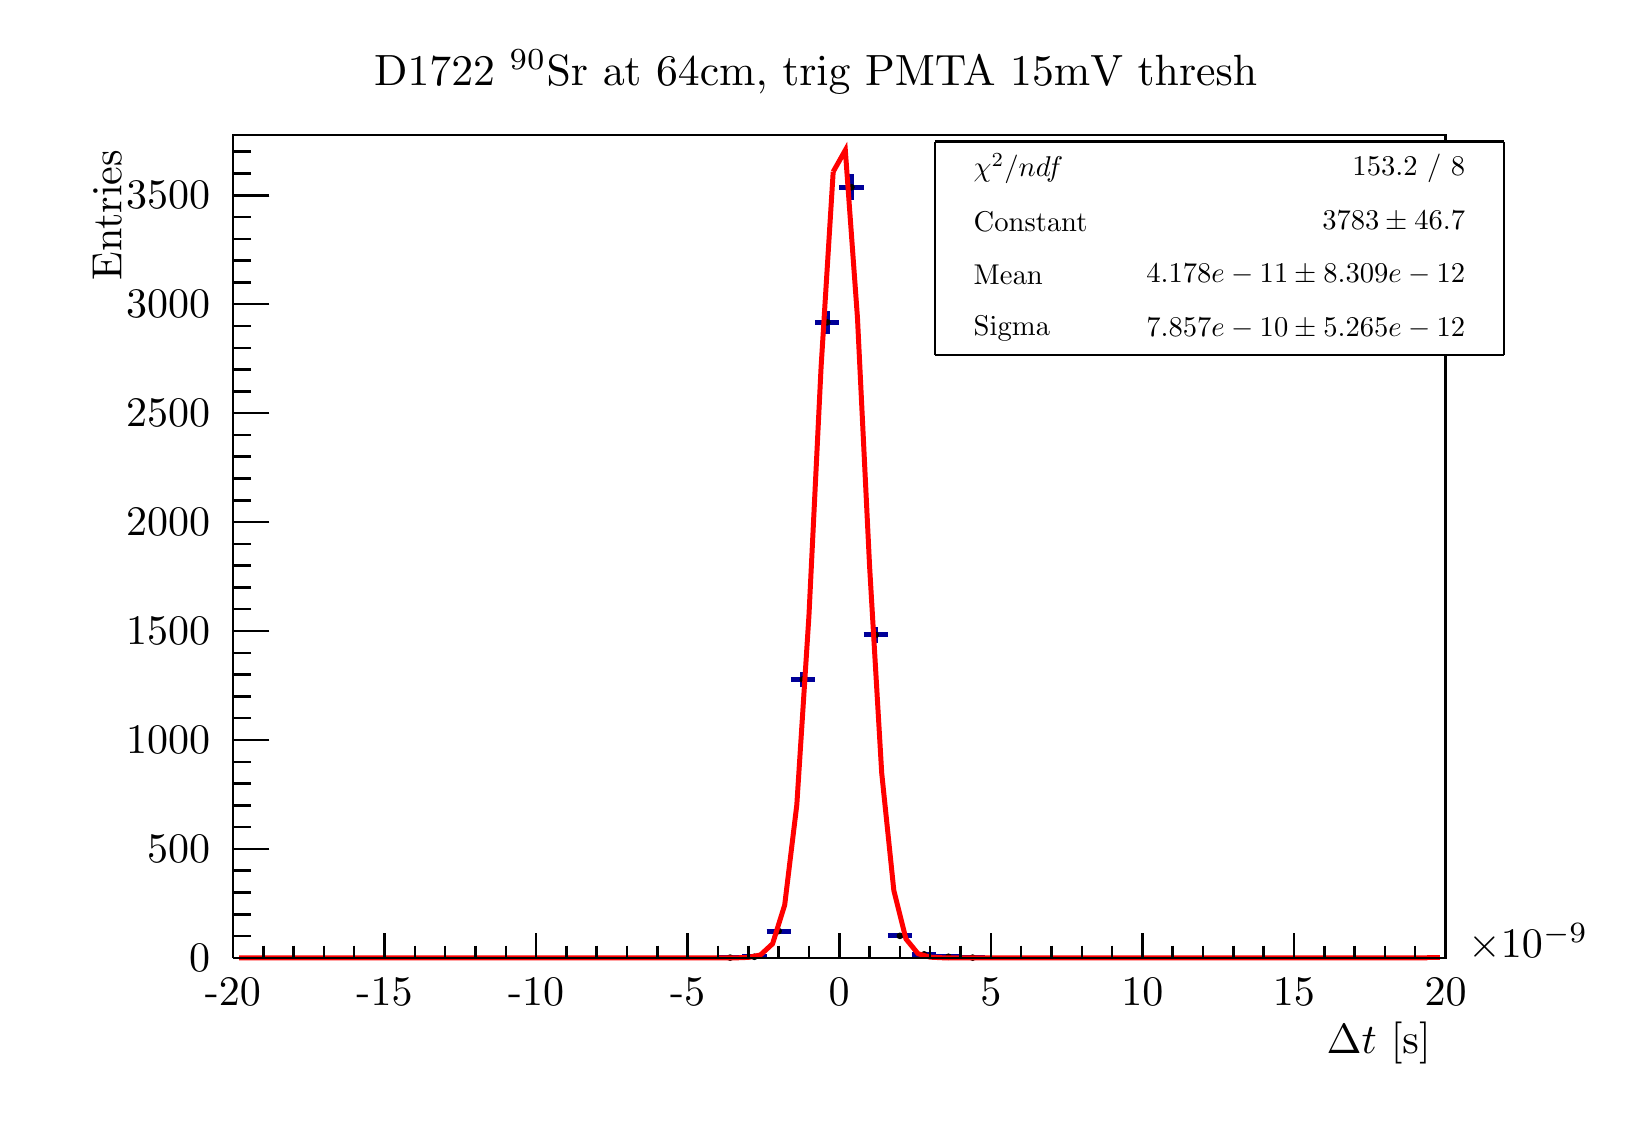
\begin{tikzpicture}
\pgfdeclareplotmark{cross} {
\pgfpathmoveto{\pgfpoint{-0.3\pgfplotmarksize}{\pgfplotmarksize}}
\pgfpathlineto{\pgfpoint{+0.3\pgfplotmarksize}{\pgfplotmarksize}}
\pgfpathlineto{\pgfpoint{+0.3\pgfplotmarksize}{0.3\pgfplotmarksize}}
\pgfpathlineto{\pgfpoint{+1\pgfplotmarksize}{0.3\pgfplotmarksize}}
\pgfpathlineto{\pgfpoint{+1\pgfplotmarksize}{-0.3\pgfplotmarksize}}
\pgfpathlineto{\pgfpoint{+0.3\pgfplotmarksize}{-0.3\pgfplotmarksize}}
\pgfpathlineto{\pgfpoint{+0.3\pgfplotmarksize}{-1.\pgfplotmarksize}}
\pgfpathlineto{\pgfpoint{-0.3\pgfplotmarksize}{-1.\pgfplotmarksize}}
\pgfpathlineto{\pgfpoint{-0.3\pgfplotmarksize}{-0.3\pgfplotmarksize}}
\pgfpathlineto{\pgfpoint{-1.\pgfplotmarksize}{-0.3\pgfplotmarksize}}
\pgfpathlineto{\pgfpoint{-1.\pgfplotmarksize}{0.3\pgfplotmarksize}}
\pgfpathlineto{\pgfpoint{-0.3\pgfplotmarksize}{0.3\pgfplotmarksize}}
\pgfpathclose
\pgfusepathqstroke
}
\pgfdeclareplotmark{cross*} {
\pgfpathmoveto{\pgfpoint{-0.3\pgfplotmarksize}{\pgfplotmarksize}}
\pgfpathlineto{\pgfpoint{+0.3\pgfplotmarksize}{\pgfplotmarksize}}
\pgfpathlineto{\pgfpoint{+0.3\pgfplotmarksize}{0.3\pgfplotmarksize}}
\pgfpathlineto{\pgfpoint{+1\pgfplotmarksize}{0.3\pgfplotmarksize}}
\pgfpathlineto{\pgfpoint{+1\pgfplotmarksize}{-0.3\pgfplotmarksize}}
\pgfpathlineto{\pgfpoint{+0.3\pgfplotmarksize}{-0.3\pgfplotmarksize}}
\pgfpathlineto{\pgfpoint{+0.3\pgfplotmarksize}{-1.\pgfplotmarksize}}
\pgfpathlineto{\pgfpoint{-0.3\pgfplotmarksize}{-1.\pgfplotmarksize}}
\pgfpathlineto{\pgfpoint{-0.3\pgfplotmarksize}{-0.3\pgfplotmarksize}}
\pgfpathlineto{\pgfpoint{-1.\pgfplotmarksize}{-0.3\pgfplotmarksize}}
\pgfpathlineto{\pgfpoint{-1.\pgfplotmarksize}{0.3\pgfplotmarksize}}
\pgfpathlineto{\pgfpoint{-0.3\pgfplotmarksize}{0.3\pgfplotmarksize}}
\pgfpathclose
\pgfusepathqfillstroke
}
\pgfdeclareplotmark{newstar} {
\pgfpathmoveto{\pgfqpoint{0pt}{\pgfplotmarksize}}
\pgfpathlineto{\pgfqpointpolar{44}{0.5\pgfplotmarksize}}
\pgfpathlineto{\pgfqpointpolar{18}{\pgfplotmarksize}}
\pgfpathlineto{\pgfqpointpolar{-20}{0.5\pgfplotmarksize}}
\pgfpathlineto{\pgfqpointpolar{-54}{\pgfplotmarksize}}
\pgfpathlineto{\pgfqpointpolar{-90}{0.5\pgfplotmarksize}}
\pgfpathlineto{\pgfqpointpolar{234}{\pgfplotmarksize}}
\pgfpathlineto{\pgfqpointpolar{198}{0.5\pgfplotmarksize}}
\pgfpathlineto{\pgfqpointpolar{162}{\pgfplotmarksize}}
\pgfpathlineto{\pgfqpointpolar{134}{0.5\pgfplotmarksize}}
\pgfpathclose
\pgfusepathqstroke
}
\pgfdeclareplotmark{newstar*} {
\pgfpathmoveto{\pgfqpoint{0pt}{\pgfplotmarksize}}
\pgfpathlineto{\pgfqpointpolar{44}{0.5\pgfplotmarksize}}
\pgfpathlineto{\pgfqpointpolar{18}{\pgfplotmarksize}}
\pgfpathlineto{\pgfqpointpolar{-20}{0.5\pgfplotmarksize}}
\pgfpathlineto{\pgfqpointpolar{-54}{\pgfplotmarksize}}
\pgfpathlineto{\pgfqpointpolar{-90}{0.5\pgfplotmarksize}}
\pgfpathlineto{\pgfqpointpolar{234}{\pgfplotmarksize}}
\pgfpathlineto{\pgfqpointpolar{198}{0.5\pgfplotmarksize}}
\pgfpathlineto{\pgfqpointpolar{162}{\pgfplotmarksize}}
\pgfpathlineto{\pgfqpointpolar{134}{0.5\pgfplotmarksize}}
\pgfpathclose
\pgfusepathqfillstroke
}
\definecolor{c}{rgb}{1,1,1};
\draw [color=c, fill=c] (0,0) rectangle (20,13.5705);
\draw [color=c, fill=c] (2.6,1.76416) rectangle (18,12.2134);
\definecolor{c}{rgb}{0,0,0};
\draw [c,line width=0.9] (2.6,1.76416) -- (2.6,12.2134) -- (18,12.2134) -- (18,1.76416) -- (2.6,1.76416);
\definecolor{c}{rgb}{1,1,1};
\draw [color=c, fill=c] (2.6,1.76416) rectangle (18,12.2134);
\definecolor{c}{rgb}{0,0,0};
\draw [c,line width=0.9] (2.6,1.76416) -- (2.6,12.2134) -- (18,12.2134) -- (18,1.76416) -- (2.6,1.76416);
\definecolor{c}{rgb}{0,0,0.6};
\draw [c,line width=1.8] (8.914,1.76416) -- (8.914,1.76693);
\draw [c,line width=1.8] (8.914,1.76693) -- (8.914,1.76969);
\draw [c,line width=1.8] (8.76,1.76693) -- (8.914,1.76693);
\draw [c,line width=1.8] (8.914,1.76693) -- (9.068,1.76693);
\definecolor{c}{rgb}{0,0,0};
\foreach \P in {(8.914,1.76693)}{\draw[mark options={color=c,fill=c},mark size=2.402402pt,mark=*,mark size=1pt] plot coordinates {\P};}
\definecolor{c}{rgb}{0,0,0.6};
\draw [c,line width=1.8] (9.222,1.77181) -- (9.222,1.77799);
\draw [c,line width=1.8] (9.222,1.77799) -- (9.222,1.78418);
\draw [c,line width=1.8] (9.068,1.77799) -- (9.222,1.77799);
\draw [c,line width=1.8] (9.222,1.77799) -- (9.376,1.77799);
\definecolor{c}{rgb}{0,0,0};
\foreach \P in {(9.222,1.77799)}{\draw[mark options={color=c,fill=c},mark size=2.402402pt,mark=*,mark size=1pt] plot coordinates {\P};}
\definecolor{c}{rgb}{0,0,0.6};
\draw [c,line width=1.8] (9.53,2.07382) -- (9.53,2.10451);
\draw [c,line width=1.8] (9.53,2.10451) -- (9.53,2.1352);
\draw [c,line width=1.8] (9.376,2.10451) -- (9.53,2.10451);
\draw [c,line width=1.8] (9.53,2.10451) -- (9.684,2.10451);
\definecolor{c}{rgb}{0,0,0};
\foreach \P in {(9.53,2.10451)}{\draw[mark options={color=c,fill=c},mark size=2.402402pt,mark=*,mark size=1pt] plot coordinates {\P};}
\definecolor{c}{rgb}{0,0,0.6};
\draw [c,line width=1.8] (9.838,5.20154) -- (9.838,5.30046);
\draw [c,line width=1.8] (9.838,5.30046) -- (9.838,5.39938);
\draw [c,line width=1.8] (9.684,5.30046) -- (9.838,5.30046);
\draw [c,line width=1.8] (9.838,5.30046) -- (9.992,5.30046);
\definecolor{c}{rgb}{0,0,0};
\foreach \P in {(9.838,5.30046)}{\draw[mark options={color=c,fill=c},mark size=2.402402pt,mark=*,mark size=1pt] plot coordinates {\P};}
\definecolor{c}{rgb}{0,0,0.6};
\draw [c,line width=1.8] (10.146,9.68623) -- (10.146,9.83568);
\draw [c,line width=1.8] (10.146,9.83568) -- (10.146,9.98513);
\draw [c,line width=1.8] (9.992,9.83568) -- (10.146,9.83568);
\draw [c,line width=1.8] (10.146,9.83568) -- (10.3,9.83568);
\definecolor{c}{rgb}{0,0,0};
\foreach \P in {(10.146,9.83568)}{\draw[mark options={color=c,fill=c},mark size=2.402402pt,mark=*,mark size=1pt] plot coordinates {\P};}
\definecolor{c}{rgb}{0,0,0.6};
\draw [c,line width=1.8] (10.454,11.3867) -- (10.454,11.5513);
\draw [c,line width=1.8] (10.454,11.5513) -- (10.454,11.7158);
\draw [c,line width=1.8] (10.3,11.5513) -- (10.454,11.5513);
\draw [c,line width=1.8] (10.454,11.5513) -- (10.608,11.5513);
\definecolor{c}{rgb}{0,0,0};
\foreach \P in {(10.454,11.5513)}{\draw[mark options={color=c,fill=c},mark size=2.402402pt,mark=*,mark size=1pt] plot coordinates {\P};}
\definecolor{c}{rgb}{0,0,0.6};
\draw [c,line width=1.8] (10.762,5.75842) -- (10.762,5.86495);
\draw [c,line width=1.8] (10.762,5.86495) -- (10.762,5.97147);
\draw [c,line width=1.8] (10.608,5.86495) -- (10.762,5.86495);
\draw [c,line width=1.8] (10.762,5.86495) -- (10.916,5.86495);
\definecolor{c}{rgb}{0,0,0};
\foreach \P in {(10.762,5.86495)}{\draw[mark options={color=c,fill=c},mark size=2.402402pt,mark=*,mark size=1pt] plot coordinates {\P};}
\definecolor{c}{rgb}{0,0,0.6};
\draw [c,line width=1.8] (11.07,2.01582) -- (11.07,2.04363);
\draw [c,line width=1.8] (11.07,2.04363) -- (11.07,2.07144);
\draw [c,line width=1.8] (10.916,2.04363) -- (11.07,2.04363);
\draw [c,line width=1.8] (11.07,2.04363) -- (11.224,2.04363);
\definecolor{c}{rgb}{0,0,0};
\foreach \P in {(11.07,2.04363)}{\draw[mark options={color=c,fill=c},mark size=2.402402pt,mark=*,mark size=1pt] plot coordinates {\P};}
\definecolor{c}{rgb}{0,0,0.6};
\draw [c,line width=1.8] (11.378,1.79736) -- (11.378,1.80843);
\draw [c,line width=1.8] (11.378,1.80843) -- (11.378,1.8195);
\draw [c,line width=1.8] (11.224,1.80843) -- (11.378,1.80843);
\draw [c,line width=1.8] (11.378,1.80843) -- (11.532,1.80843);
\definecolor{c}{rgb}{0,0,0};
\foreach \P in {(11.378,1.80843)}{\draw[mark options={color=c,fill=c},mark size=2.402402pt,mark=*,mark size=1pt] plot coordinates {\P};}
\definecolor{c}{rgb}{0,0,0.6};
\draw [c,line width=1.8] (11.686,1.77181) -- (11.686,1.77799);
\draw [c,line width=1.8] (11.686,1.77799) -- (11.686,1.78418);
\draw [c,line width=1.8] (11.532,1.77799) -- (11.686,1.77799);
\draw [c,line width=1.8] (11.686,1.77799) -- (11.84,1.77799);
\definecolor{c}{rgb}{0,0,0};
\foreach \P in {(11.686,1.77799)}{\draw[mark options={color=c,fill=c},mark size=2.402402pt,mark=*,mark size=1pt] plot coordinates {\P};}
\definecolor{c}{rgb}{0,0,0.6};
\draw [c,line width=1.8] (11.994,1.76416) -- (11.994,1.76693);
\draw [c,line width=1.8] (11.994,1.76693) -- (11.994,1.76969);
\draw [c,line width=1.8] (11.84,1.76693) -- (11.994,1.76693);
\draw [c,line width=1.8] (11.994,1.76693) -- (12.148,1.76693);
\definecolor{c}{rgb}{0,0,0};
\foreach \P in {(11.994,1.76693)}{\draw[mark options={color=c,fill=c},mark size=2.402402pt,mark=*,mark size=1pt] plot coordinates {\P};}
\definecolor{c}{rgb}{1,0,0};
\draw [c,line width=1.8] (2.677,1.76416) -- (2.831,1.76416) -- (2.985,1.76416) -- (3.139,1.76416) -- (3.293,1.76416) -- (3.447,1.76416) -- (3.601,1.76416) -- (3.755,1.76416) -- (3.909,1.76416) -- (4.063,1.76416) -- (4.217,1.76416) -- (4.371,1.76416)
 -- (4.525,1.76416) -- (4.679,1.76416) -- (4.833,1.76416) -- (4.987,1.76416) -- (5.141,1.76416) -- (5.295,1.76416) -- (5.449,1.76416) -- (5.603,1.76416) -- (5.757,1.76416) -- (5.911,1.76416) -- (6.065,1.76416) -- (6.219,1.76416) -- (6.373,1.76416) --
 (6.527,1.76416) -- (6.681,1.76416) -- (6.835,1.76416) -- (6.989,1.76416) -- (7.143,1.76416) -- (7.297,1.76416) -- (7.451,1.76416) -- (7.605,1.76416) -- (7.759,1.76416) -- (7.913,1.76416) -- (8.067,1.76416) -- (8.221,1.76416) -- (8.375,1.76416) --
 (8.529,1.76416) -- (8.683,1.76416) -- (8.837,1.76416) -- (8.991,1.76416) -- (9.145,1.76998) -- (9.299,1.80089) -- (9.453,1.94285) -- (9.607,2.43506) -- (9.761,3.70796) -- (9.915,6.11015) -- (10.069,9.26248) -- (10.223,11.7476);
\draw [c,line width=1.8] (10.223,11.7476) -- (10.377,12.0215) -- (10.531,9.89679) -- (10.685,6.74) -- (10.839,4.11347) -- (10.993,2.62012) -- (11.147,2.00482) -- (11.301,1.81637) -- (11.455,1.7729) -- (11.609,1.76529) -- (11.763,1.76416) --
 (11.917,1.76416) -- (12.071,1.76416) -- (12.225,1.76416) -- (12.379,1.76416) -- (12.533,1.76416) -- (12.687,1.76416) -- (12.841,1.76416) -- (12.995,1.76416) -- (13.149,1.76416) -- (13.303,1.76416) -- (13.457,1.76416) -- (13.611,1.76416) --
 (13.765,1.76416) -- (13.919,1.76416) -- (14.073,1.76416) -- (14.227,1.76416) -- (14.381,1.76416) -- (14.535,1.76416) -- (14.689,1.76416) -- (14.843,1.76416) -- (14.997,1.76416) -- (15.151,1.76416) -- (15.305,1.76416) -- (15.459,1.76416) --
 (15.613,1.76416) -- (15.767,1.76416) -- (15.921,1.76416) -- (16.075,1.76416) -- (16.229,1.76416) -- (16.383,1.76416) -- (16.537,1.76416) -- (16.691,1.76416) -- (16.845,1.76416) -- (16.999,1.76416) -- (17.153,1.76416) -- (17.307,1.76416) --
 (17.461,1.76416) -- (17.615,1.76416) -- (17.769,1.76416);
\draw [c,line width=1.8] (17.769,1.76416) -- (17.923,1.76416);
\definecolor{c}{rgb}{1,1,1};
\draw [color=c, fill=c] (11.5186,9.42152) rectangle (18.7393,12.1299);
\definecolor{c}{rgb}{0,0,0};
\draw [c,line width=0.9] (11.5186,9.42152) -- (18.7393,9.42152);
\draw [c,line width=0.9] (18.7393,9.42152) -- (18.7393,12.1299);
\draw [c,line width=0.9] (18.7393,12.1299) -- (11.5186,12.1299);
\draw [c,line width=0.9] (11.5186,12.1299) -- (11.5186,9.42152);
\draw [anchor= west] (11.8797,11.7913) node[scale=1.03301, color=c, rotate=0]{$\chi^{2} / ndf $};
\draw [anchor= east] (18.3782,11.7913) node[scale=1.03301, color=c, rotate=0]{ 153.2 / 8};
\draw [anchor= west] (11.8797,11.1142) node[scale=1.03301, color=c, rotate=0]{Constant };
\draw [anchor= east] (18.3782,11.1142) node[scale=1.03301, color=c, rotate=0]{$  3783 \pm 46.7$};
\draw [anchor= west] (11.8797,10.4371) node[scale=1.03301, color=c, rotate=0]{Mean     };
\draw [anchor= east] (18.3782,10.4371) node[scale=1.03301, color=c, rotate=0]{$ 4.178e-11 \pm 8.309e-12$};
\draw [anchor= west] (11.8797,9.76007) node[scale=1.03301, color=c, rotate=0]{Sigma    };
\draw [anchor= east] (18.3782,9.76007) node[scale=1.03301, color=c, rotate=0]{$ 7.857e-10 \pm 5.265e-12$};
\draw [c,line width=0.9] (2.6,1.76416) -- (18,1.76416);
\draw [c,line width=0.9] (2.6,2.07764) -- (2.6,1.76416);
\draw [c,line width=0.9] (2.985,1.9209) -- (2.985,1.76416);
\draw [c,line width=0.9] (3.37,1.9209) -- (3.37,1.76416);
\draw [c,line width=0.9] (3.755,1.9209) -- (3.755,1.76416);
\draw [c,line width=0.9] (4.14,1.9209) -- (4.14,1.76416);
\draw [c,line width=0.9] (4.525,2.07764) -- (4.525,1.76416);
\draw [c,line width=0.9] (4.91,1.9209) -- (4.91,1.76416);
\draw [c,line width=0.9] (5.295,1.9209) -- (5.295,1.76416);
\draw [c,line width=0.9] (5.68,1.9209) -- (5.68,1.76416);
\draw [c,line width=0.9] (6.065,1.9209) -- (6.065,1.76416);
\draw [c,line width=0.9] (6.45,2.07764) -- (6.45,1.76416);
\draw [c,line width=0.9] (6.835,1.9209) -- (6.835,1.76416);
\draw [c,line width=0.9] (7.22,1.9209) -- (7.22,1.76416);
\draw [c,line width=0.9] (7.605,1.9209) -- (7.605,1.76416);
\draw [c,line width=0.9] (7.99,1.9209) -- (7.99,1.76416);
\draw [c,line width=0.9] (8.375,2.07764) -- (8.375,1.76416);
\draw [c,line width=0.9] (8.76,1.9209) -- (8.76,1.76416);
\draw [c,line width=0.9] (9.145,1.9209) -- (9.145,1.76416);
\draw [c,line width=0.9] (9.53,1.9209) -- (9.53,1.76416);
\draw [c,line width=0.9] (9.915,1.9209) -- (9.915,1.76416);
\draw [c,line width=0.9] (10.3,2.07764) -- (10.3,1.76416);
\draw [c,line width=0.9] (10.685,1.9209) -- (10.685,1.76416);
\draw [c,line width=0.9] (11.07,1.9209) -- (11.07,1.76416);
\draw [c,line width=0.9] (11.455,1.9209) -- (11.455,1.76416);
\draw [c,line width=0.9] (11.84,1.9209) -- (11.84,1.76416);
\draw [c,line width=0.9] (12.225,2.07764) -- (12.225,1.76416);
\draw [c,line width=0.9] (12.61,1.9209) -- (12.61,1.76416);
\draw [c,line width=0.9] (12.995,1.9209) -- (12.995,1.76416);
\draw [c,line width=0.9] (13.38,1.9209) -- (13.38,1.76416);
\draw [c,line width=0.9] (13.765,1.9209) -- (13.765,1.76416);
\draw [c,line width=0.9] (14.15,2.07764) -- (14.15,1.76416);
\draw [c,line width=0.9] (14.535,1.9209) -- (14.535,1.76416);
\draw [c,line width=0.9] (14.92,1.9209) -- (14.92,1.76416);
\draw [c,line width=0.9] (15.305,1.9209) -- (15.305,1.76416);
\draw [c,line width=0.9] (15.69,1.9209) -- (15.69,1.76416);
\draw [c,line width=0.9] (16.075,2.07764) -- (16.075,1.76416);
\draw [c,line width=0.9] (16.46,1.9209) -- (16.46,1.76416);
\draw [c,line width=0.9] (16.845,1.9209) -- (16.845,1.76416);
\draw [c,line width=0.9] (17.23,1.9209) -- (17.23,1.76416);
\draw [c,line width=0.9] (17.615,1.9209) -- (17.615,1.76416);
\draw [c,line width=0.9] (18,2.07764) -- (18,1.76416);
\draw [anchor=base] (2.6,1.15349) node[scale=1.51913, color=c, rotate=0]{-20};
\draw [anchor=base] (4.525,1.15349) node[scale=1.51913, color=c, rotate=0]{-15};
\draw [anchor=base] (6.45,1.15349) node[scale=1.51913, color=c, rotate=0]{-10};
\draw [anchor=base] (8.375,1.15349) node[scale=1.51913, color=c, rotate=0]{-5};
\draw [anchor=base] (10.3,1.15349) node[scale=1.51913, color=c, rotate=0]{0};
\draw [anchor=base] (12.225,1.15349) node[scale=1.51913, color=c, rotate=0]{5};
\draw [anchor=base] (14.15,1.15349) node[scale=1.51913, color=c, rotate=0]{10};
\draw [anchor=base] (16.075,1.15349) node[scale=1.51913, color=c, rotate=0]{15};
\draw [anchor=base] (18,1.15349) node[scale=1.51913, color=c, rotate=0]{20};
\draw [anchor=base west] (18.1,1.76416) node[scale=1.51913, color=c, rotate=0]{$\times10^{-9}$};
\draw [anchor= east] (18,0.678523) node[scale=1.51913, color=c, rotate=0]{$\Delta t$ [s]};
\draw [c,line width=0.9] (2.6,1.76416) -- (2.6,12.2134);
\draw [c,line width=0.9] (3.062,1.76416) -- (2.6,1.76416);
\draw [c,line width=0.9] (2.831,2.04086) -- (2.6,2.04086);
\draw [c,line width=0.9] (2.831,2.31757) -- (2.6,2.31757);
\draw [c,line width=0.9] (2.831,2.59428) -- (2.6,2.59428);
\draw [c,line width=0.9] (2.831,2.87098) -- (2.6,2.87098);
\draw [c,line width=0.9] (3.062,3.14769) -- (2.6,3.14769);
\draw [c,line width=0.9] (2.831,3.4244) -- (2.6,3.4244);
\draw [c,line width=0.9] (2.831,3.7011) -- (2.6,3.7011);
\draw [c,line width=0.9] (2.831,3.97781) -- (2.6,3.97781);
\draw [c,line width=0.9] (2.831,4.25451) -- (2.6,4.25451);
\draw [c,line width=0.9] (3.062,4.53122) -- (2.6,4.53122);
\draw [c,line width=0.9] (2.831,4.80793) -- (2.6,4.80793);
\draw [c,line width=0.9] (2.831,5.08463) -- (2.6,5.08463);
\draw [c,line width=0.9] (2.831,5.36134) -- (2.6,5.36134);
\draw [c,line width=0.9] (2.831,5.63805) -- (2.6,5.63805);
\draw [c,line width=0.9] (3.062,5.91475) -- (2.6,5.91475);
\draw [c,line width=0.9] (2.831,6.19146) -- (2.6,6.19146);
\draw [c,line width=0.9] (2.831,6.46816) -- (2.6,6.46816);
\draw [c,line width=0.9] (2.831,6.74487) -- (2.6,6.74487);
\draw [c,line width=0.9] (2.831,7.02158) -- (2.6,7.02158);
\draw [c,line width=0.9] (3.062,7.29828) -- (2.6,7.29828);
\draw [c,line width=0.9] (2.831,7.57499) -- (2.6,7.57499);
\draw [c,line width=0.9] (2.831,7.8517) -- (2.6,7.8517);
\draw [c,line width=0.9] (2.831,8.1284) -- (2.6,8.1284);
\draw [c,line width=0.9] (2.831,8.40511) -- (2.6,8.40511);
\draw [c,line width=0.9] (3.062,8.68182) -- (2.6,8.68182);
\draw [c,line width=0.9] (2.831,8.95852) -- (2.6,8.95852);
\draw [c,line width=0.9] (2.831,9.23523) -- (2.6,9.23523);
\draw [c,line width=0.9] (2.831,9.51193) -- (2.6,9.51193);
\draw [c,line width=0.9] (2.831,9.78864) -- (2.6,9.78864);
\draw [c,line width=0.9] (3.062,10.0653) -- (2.6,10.0653);
\draw [c,line width=0.9] (2.831,10.3421) -- (2.6,10.3421);
\draw [c,line width=0.9] (2.831,10.6188) -- (2.6,10.6188);
\draw [c,line width=0.9] (2.831,10.8955) -- (2.6,10.8955);
\draw [c,line width=0.9] (2.831,11.1722) -- (2.6,11.1722);
\draw [c,line width=0.9] (3.062,11.4489) -- (2.6,11.4489);
\draw [c,line width=0.9] (3.062,11.4489) -- (2.6,11.4489);
\draw [c,line width=0.9] (2.831,11.7256) -- (2.6,11.7256);
\draw [c,line width=0.9] (2.831,12.0023) -- (2.6,12.0023);
\draw [anchor= east] (2.5,1.76416) node[scale=1.51913, color=c, rotate=0]{0};
\draw [anchor= east] (2.5,3.14769) node[scale=1.51913, color=c, rotate=0]{500};
\draw [anchor= east] (2.5,4.53122) node[scale=1.51913, color=c, rotate=0]{1000};
\draw [anchor= east] (2.5,5.91475) node[scale=1.51913, color=c, rotate=0]{1500};
\draw [anchor= east] (2.5,7.29828) node[scale=1.51913, color=c, rotate=0]{2000};
\draw [anchor= east] (2.5,8.68182) node[scale=1.51913, color=c, rotate=0]{2500};
\draw [anchor= east] (2.5,10.0653) node[scale=1.51913, color=c, rotate=0]{3000};
\draw [anchor= east] (2.5,11.4489) node[scale=1.51913, color=c, rotate=0]{3500};
\draw [anchor= east] (1,12.2134) node[scale=1.51913, color=c, rotate=90]{Entries};
\definecolor{c}{rgb}{1,1,1};
\draw [color=c, fill=c] (11.5186,9.42152) rectangle (18.7393,12.1299);
\definecolor{c}{rgb}{0,0,0};
\draw [c,line width=0.9] (11.5186,9.42152) -- (18.7393,9.42152);
\draw [c,line width=0.9] (18.7393,9.42152) -- (18.7393,12.1299);
\draw [c,line width=0.9] (18.7393,12.1299) -- (11.5186,12.1299);
\draw [c,line width=0.9] (11.5186,12.1299) -- (11.5186,9.42152);
\draw [anchor= west] (11.8797,11.7913) node[scale=1.03301, color=c, rotate=0]{$\chi^{2} / ndf $};
\draw [anchor= east] (18.3782,11.7913) node[scale=1.03301, color=c, rotate=0]{ 153.2 / 8};
\draw [anchor= west] (11.8797,11.1142) node[scale=1.03301, color=c, rotate=0]{Constant };
\draw [anchor= east] (18.3782,11.1142) node[scale=1.03301, color=c, rotate=0]{$  3783 \pm 46.7$};
\draw [anchor= west] (11.8797,10.4371) node[scale=1.03301, color=c, rotate=0]{Mean     };
\draw [anchor= east] (18.3782,10.4371) node[scale=1.03301, color=c, rotate=0]{$ 4.178e-11 \pm 8.309e-12$};
\draw [anchor= west] (11.8797,9.76007) node[scale=1.03301, color=c, rotate=0]{Sigma    };
\draw [anchor= east] (18.3782,9.76007) node[scale=1.03301, color=c, rotate=0]{$ 7.857e-10 \pm 5.265e-12$};
\draw (10,13.0186) node[scale=1.5799, color=c, rotate=0]{D1722 $^{90}$Sr at 64cm, trig PMTA 15mV thresh};
\end{tikzpicture}

	\end{adjustbox}
	\caption{Difference in signal arrival time PMTs at each end of a bar as measured using a $^{90}$Sr source placed 64~cm from one end of the bar.}
	\label{fig:s4Res}	
\end{figure}

\begin{figure}[ht]    
  \begin{minipage}[t]{.48\textwidth}
    \centering
    \includegraphics[width=0.6\linewidth]{files/Figures/dstofFront.png}
    \caption{Front view of the downstream time of flight system}
    \label{fig:dstofFront}
  \end{minipage}
  \hspace{0.3cm}
  \begin{minipage}[t]{.48\textwidth}
    \centering
    \includegraphics[width=0.45\linewidth]{files/Figures/dstofDiag.png}
    \caption{Diagonal view of the downstream time of flight system showing more clearly the two rows of scintillator bars and photomultiplier tubes}
    \label{fig:dstofDiagonal}
  \end{minipage}
\end{figure}

The anode signals of all 20 of the PMTs are discriminated using LeCroy 620AL NIM discriminators, at a threshold of 20~mV.
The discriminated signals are then fed into a time-to-digital converter. A signal in $\mathit{S4}$ is deemed to have occurred if a signal is seen in both PMTs, above the discriminator threshold, on the same bar within 20~ns of each other. 
This timing window is determined through testing performed with a $^{90}$Sr source at known positions on the bar.

The $\mathit{S1-S2}$ coincidence signal is digitized by the same time-to-digital converter. This signal is used to calculate the particle time of flight from $\mathit{S2}$ to $\mathit{S4}$.

\subsection{The HPTPC Prototype}
The steel vessel is rated to 6~barA of pressure, and the walls of the vessel are 1~cm thick.
The TPC comprised thin steel mesh electrodes (one cathode and three anodes), and 12 copper rings to create the uniform drift field.
The drift distance produced was 48~cm, with the anodes separated by 1~mm. Data taking with the TPC made use of both optical and charge readout.
The vessel, electrodes, and drift region of the TPC are shown in figure~\ref{fig:TPC}.

\begin{figure}
  \centering
  \includegraphics[width=0.6\linewidth]{files/Figures/IMG_1194.jpg}
  \caption{Cross-sectional view of the TPC; the thin mesh electrodes and copper ring drift volume can be seen inside the steel vessel}
  \label{fig:TPC}
  \todo[inline]{TOBY: "A head on shot would show the relevant information better."}
  \todo[inline]{TOBY: "This caption needs to give the important quantitative info for the ToF analysis, eg. wall thickness, separation of walls at the height of the beam centre, the distance from the inside of the upstream wall to the drift region, etc"}
\end{figure}

%The centre of the TPC was placed 13~m from the beam entrance with \textit{S3} and \textit{S4} directly upstream and downstream of the vessel, respectively. 
In the coordinate system shown in Figure~\ref{fig:setup}, the TPC centre lies at $X=10.82~\text{m}$, $Y=0.5593~\text{m}$, $Z=-0.0114~\text{m}$. 
\todo[inline]{Description of coordinate system needs to go in to make this clear.}
Throughout the run, the TPC was filled with either pure argon, or a combination of argon and a small percentage of quencher. 
The performance of this TPC is the subject of a forthcoming publication.

\section{Analysis}
\label{hptpcPaper:sec:Analysis}
\subsection{Analysis Goals}

The primary aims of the use of $\mathit{S1} - \mathit{S4}$ were as follows: to assess the feasibility of using this combination of off-axis positioning and a moderated beam at the PS to produce the momenta of most relevance to neutrino cross-section studies and to characterize the incident flux on the TPC and exiting the TPC, for the TPC data analysis. \todo[inline]{TOBY, I rewrote this paragraph in line with the comments. This ok with you?}

%Protons take longer to travel the distance from \textit{S1} to \textit{S3} or \textit{S4} than lighter particles that are close to being minimum ionising.
%This difference in time of flight can be used to distinguish between the two types of particles.
%Distinguishing these MIPs from one another is more difficult due to their similar masses and can be only determined by the upstream ToF system.
%From the particle flux data, it is possible to measure the ratio of protons to other particles over the range of off-axis angles covered by the \textit{S3} and \textit{S4} walls, and for varying numbers of moderator blocks.

A particle of mass $m$ with momentum $p$ travelling over a distance $d$ will traverse said distance in a time
\begin{align}
	t = d \sqrt{\frac{m^2}{p^2} + \frac{1}{c^2}}
\end{align}
where $c$ is the speed of light in a vacuum.
Therefore, particles with a greater momentum or smaller mass will cross the same distance in a shorter time.
This means that, if there exists a beam of particles of different species but with the same momenta (as is produced by the PS), the mass of of a particle can be determined by measuring this time of flight, $t$.

For example, a charged pion with a momentum of 0.8~GeV/c will have a time of flight from $\mathit{S1}$ to $\mathit{S3}$ (a distance of 10.9~m) of 37~ns, while a proton with the same momentum will have a time of flight of 56~ns.
For the same two particles travelling between $\mathit{S2}$ and $\mathit{S4}$ (a distance of 12.6~m), the charged pion would have a time of flight of 43~ns and the proton would have a time of flight of 65~ns.
\todo[inline]{Add error bars to these numbers.}

The variation of momentum spectrum, proton-MIP ratio, and proton multiplicity with differing numbers of acrylic blocks as a function of angle off the beam axis provide the motivation for the measurement techniques used.
As such the data used in these results cover two days in the run where the number of moderator blocks was varied with other beam properties held approximately constant.
The numbers of spills per moderator block are shown in Table~\ref{tab:spills} (with more data taken for 4 blocks as that was the configuration used for the majority of the beam test).

\begin{table}
  \centering
  \begin{tabular}{|c|c|}
    \hline
    Number of moderator blocks & Recorded spills \\
    \hline
    0 & 257 \\
    1 & 254 \\
    2 & 267 \\
    3 & 220 \\
    4 & 3884 \\
    \hline
  \end{tabular}
  \caption{The number of spills recorded for each moderator block configuration}
  \label{tab:spills}
\end{table}

\subsection{Analysis Methods}

Figure~\ref{fig:s3tof} shows the time of flight spectrum recorded in the $\mathit{S3}$ timing point for varying numbers of moderator blocks.
The quicker peak is formed by minimum ionizing particles, while the peak at higher values of $\mathit{S3} - \mathit{S1}$ corresponds to protons.
The black, 0 block peak ranging from 90 to 100~ns corresponds to deuterons.
\begin{figure}[h]
  \begin{adjustbox}{max totalsize={.8\textwidth}{.5\textheight},center}
    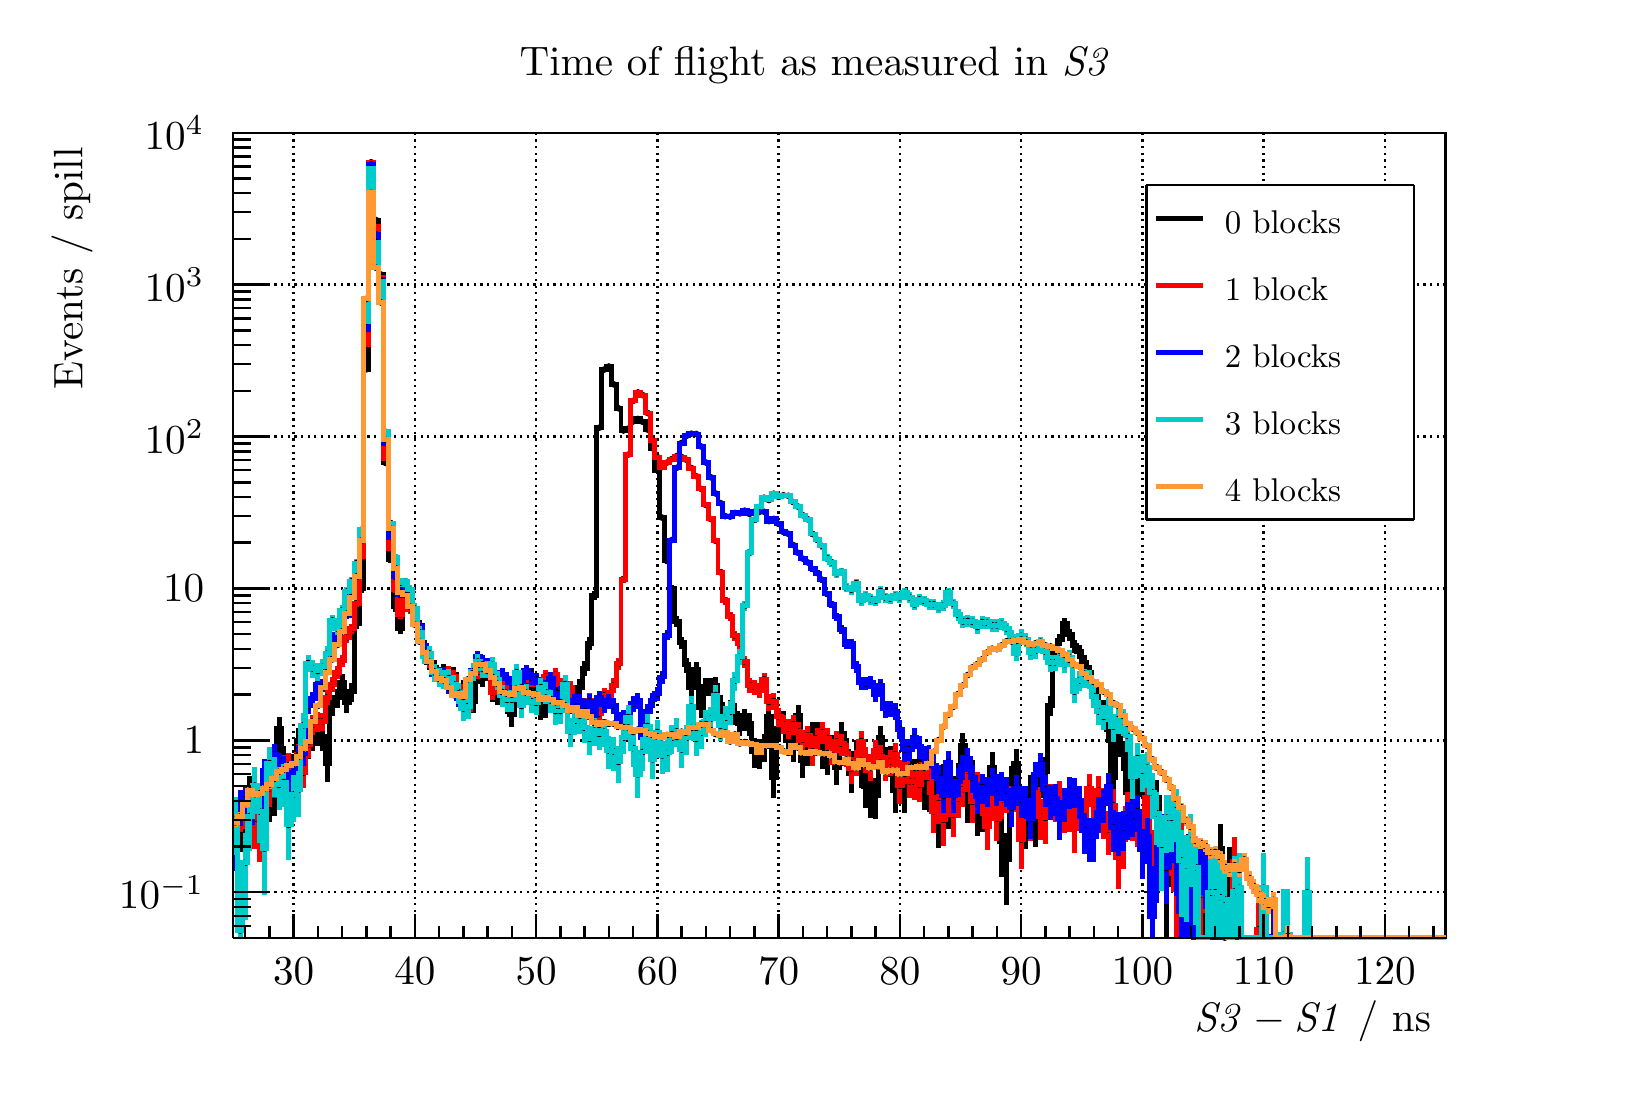
\begin{tikzpicture}
\pgfdeclareplotmark{cross} {
\pgfpathmoveto{\pgfpoint{-0.3\pgfplotmarksize}{\pgfplotmarksize}}
\pgfpathlineto{\pgfpoint{+0.3\pgfplotmarksize}{\pgfplotmarksize}}
\pgfpathlineto{\pgfpoint{+0.3\pgfplotmarksize}{0.3\pgfplotmarksize}}
\pgfpathlineto{\pgfpoint{+1\pgfplotmarksize}{0.3\pgfplotmarksize}}
\pgfpathlineto{\pgfpoint{+1\pgfplotmarksize}{-0.3\pgfplotmarksize}}
\pgfpathlineto{\pgfpoint{+0.3\pgfplotmarksize}{-0.3\pgfplotmarksize}}
\pgfpathlineto{\pgfpoint{+0.3\pgfplotmarksize}{-1.\pgfplotmarksize}}
\pgfpathlineto{\pgfpoint{-0.3\pgfplotmarksize}{-1.\pgfplotmarksize}}
\pgfpathlineto{\pgfpoint{-0.3\pgfplotmarksize}{-0.3\pgfplotmarksize}}
\pgfpathlineto{\pgfpoint{-1.\pgfplotmarksize}{-0.3\pgfplotmarksize}}
\pgfpathlineto{\pgfpoint{-1.\pgfplotmarksize}{0.3\pgfplotmarksize}}
\pgfpathlineto{\pgfpoint{-0.3\pgfplotmarksize}{0.3\pgfplotmarksize}}
\pgfpathclose
\pgfusepathqstroke
}
\pgfdeclareplotmark{cross*} {
\pgfpathmoveto{\pgfpoint{-0.3\pgfplotmarksize}{\pgfplotmarksize}}
\pgfpathlineto{\pgfpoint{+0.3\pgfplotmarksize}{\pgfplotmarksize}}
\pgfpathlineto{\pgfpoint{+0.3\pgfplotmarksize}{0.3\pgfplotmarksize}}
\pgfpathlineto{\pgfpoint{+1\pgfplotmarksize}{0.3\pgfplotmarksize}}
\pgfpathlineto{\pgfpoint{+1\pgfplotmarksize}{-0.3\pgfplotmarksize}}
\pgfpathlineto{\pgfpoint{+0.3\pgfplotmarksize}{-0.3\pgfplotmarksize}}
\pgfpathlineto{\pgfpoint{+0.3\pgfplotmarksize}{-1.\pgfplotmarksize}}
\pgfpathlineto{\pgfpoint{-0.3\pgfplotmarksize}{-1.\pgfplotmarksize}}
\pgfpathlineto{\pgfpoint{-0.3\pgfplotmarksize}{-0.3\pgfplotmarksize}}
\pgfpathlineto{\pgfpoint{-1.\pgfplotmarksize}{-0.3\pgfplotmarksize}}
\pgfpathlineto{\pgfpoint{-1.\pgfplotmarksize}{0.3\pgfplotmarksize}}
\pgfpathlineto{\pgfpoint{-0.3\pgfplotmarksize}{0.3\pgfplotmarksize}}
\pgfpathclose
\pgfusepathqfillstroke
}
\pgfdeclareplotmark{newstar} {
\pgfpathmoveto{\pgfqpoint{0pt}{\pgfplotmarksize}}
\pgfpathlineto{\pgfqpointpolar{44}{0.5\pgfplotmarksize}}
\pgfpathlineto{\pgfqpointpolar{18}{\pgfplotmarksize}}
\pgfpathlineto{\pgfqpointpolar{-20}{0.5\pgfplotmarksize}}
\pgfpathlineto{\pgfqpointpolar{-54}{\pgfplotmarksize}}
\pgfpathlineto{\pgfqpointpolar{-90}{0.5\pgfplotmarksize}}
\pgfpathlineto{\pgfqpointpolar{234}{\pgfplotmarksize}}
\pgfpathlineto{\pgfqpointpolar{198}{0.5\pgfplotmarksize}}
\pgfpathlineto{\pgfqpointpolar{162}{\pgfplotmarksize}}
\pgfpathlineto{\pgfqpointpolar{134}{0.5\pgfplotmarksize}}
\pgfpathclose
\pgfusepathqstroke
}
\pgfdeclareplotmark{newstar*} {
\pgfpathmoveto{\pgfqpoint{0pt}{\pgfplotmarksize}}
\pgfpathlineto{\pgfqpointpolar{44}{0.5\pgfplotmarksize}}
\pgfpathlineto{\pgfqpointpolar{18}{\pgfplotmarksize}}
\pgfpathlineto{\pgfqpointpolar{-20}{0.5\pgfplotmarksize}}
\pgfpathlineto{\pgfqpointpolar{-54}{\pgfplotmarksize}}
\pgfpathlineto{\pgfqpointpolar{-90}{0.5\pgfplotmarksize}}
\pgfpathlineto{\pgfqpointpolar{234}{\pgfplotmarksize}}
\pgfpathlineto{\pgfqpointpolar{198}{0.5\pgfplotmarksize}}
\pgfpathlineto{\pgfqpointpolar{162}{\pgfplotmarksize}}
\pgfpathlineto{\pgfqpointpolar{134}{0.5\pgfplotmarksize}}
\pgfpathclose
\pgfusepathqfillstroke
}
\definecolor{c}{rgb}{1,1,1};
\draw [color=c, fill=c] (0,0) rectangle (20,13.2798);
\draw [color=c, fill=c] (2.6,1.72637) rectangle (18,11.9518);
\definecolor{c}{rgb}{0,0,0};
\draw [c,line width=0.9] (2.6,1.72637) -- (2.6,11.9518) -- (18,11.9518) -- (18,1.72637) -- (2.6,1.72637);
\definecolor{c}{rgb}{1,1,1};
\draw [color=c, fill=c] (2.6,1.72637) rectangle (18,11.9518);
\definecolor{c}{rgb}{0,0,0};
\draw [c,line width=0.9] (2.6,1.72637) -- (2.6,11.9518) -- (18,11.9518) -- (18,1.72637) -- (2.6,1.72637);
\draw [c,line width=0.9] (2.6,1.72637) -- (18,1.72637);
\draw [c,dash pattern=on 0.80pt off 1.60pt ,line width=0.9] (3.37,11.9518) -- (3.37,1.72637);
\draw [c,dash pattern=on 0.80pt off 1.60pt ,line width=0.9] (4.91,11.9518) -- (4.91,1.72637);
\draw [c,dash pattern=on 0.80pt off 1.60pt ,line width=0.9] (6.45,11.9518) -- (6.45,1.72637);
\draw [c,dash pattern=on 0.80pt off 1.60pt ,line width=0.9] (7.99,11.9518) -- (7.99,1.72637);
\draw [c,dash pattern=on 0.80pt off 1.60pt ,line width=0.9] (9.53,11.9518) -- (9.53,1.72637);
\draw [c,dash pattern=on 0.80pt off 1.60pt ,line width=0.9] (11.07,11.9518) -- (11.07,1.72637);
\draw [c,dash pattern=on 0.80pt off 1.60pt ,line width=0.9] (12.61,11.9518) -- (12.61,1.72637);
\draw [c,dash pattern=on 0.80pt off 1.60pt ,line width=0.9] (14.15,11.9518) -- (14.15,1.72637);
\draw [c,dash pattern=on 0.80pt off 1.60pt ,line width=0.9] (15.69,11.9518) -- (15.69,1.72637);
\draw [c,dash pattern=on 0.80pt off 1.60pt ,line width=0.9] (17.23,11.9518) -- (17.23,1.72637);
\draw [c,dash pattern=on 0.80pt off 1.60pt ,line width=0.9] (3.37,11.9518) -- (3.37,1.72637);
\draw [c,dash pattern=on 0.80pt off 1.60pt ,line width=0.9] (17.23,11.9518) -- (17.23,1.72637);
\draw [c,line width=0.9] (2.6,1.72637) -- (2.6,11.9518);
\draw [c,dash pattern=on 0.80pt off 1.60pt ,line width=0.9] (18,2.30705) -- (2.6,2.30705);
\draw [c,dash pattern=on 0.80pt off 1.60pt ,line width=0.9] (18,4.236) -- (2.6,4.236);
\draw [c,dash pattern=on 0.80pt off 1.60pt ,line width=0.9] (18,6.16495) -- (2.6,6.16495);
\draw [c,dash pattern=on 0.80pt off 1.60pt ,line width=0.9] (18,8.0939) -- (2.6,8.0939);
\draw [c,dash pattern=on 0.80pt off 1.60pt ,line width=0.9] (18,10.0229) -- (2.6,10.0229);
\draw [c,dash pattern=on 0.80pt off 1.60pt ,line width=0.9] (18,11.9518) -- (2.6,11.9518);
\definecolor{c}{rgb}{0,0,0.6};
\draw [c,line width=0.9] (2.6,1.72637) -- (2.6616,1.72637) -- (2.6616,1.72637) -- (2.7232,1.72637) -- (2.7232,1.72637) -- (2.7848,1.72637) -- (2.7848,1.72637) -- (2.8464,1.72637) -- (2.8464,1.72637) -- (2.908,1.72637) -- (2.908,1.72637) --
 (2.9696,1.72637) -- (2.9696,1.72637) -- (3.0312,1.72637) -- (3.0312,1.72637) -- (3.0928,1.72637) -- (3.0928,1.72637) -- (3.1544,1.72637) -- (3.1544,1.72637) -- (3.216,1.72637) -- (3.216,1.72637) -- (3.2776,1.72637) -- (3.2776,1.72637) --
 (3.3392,1.72637) -- (3.3392,1.72637) -- (3.4008,1.72637) -- (3.4008,1.72637) -- (3.4624,1.72637) -- (3.4624,1.72637) -- (3.524,1.72637) -- (3.524,1.72637) -- (3.5856,1.72637) -- (3.5856,1.72637) -- (3.6472,1.72637) -- (3.6472,1.72637) --
 (3.7088,1.72637) -- (3.7088,1.72637) -- (3.7704,1.72637) -- (3.7704,1.72637) -- (3.832,1.72637) -- (3.832,1.72637) -- (3.8936,1.72637) -- (3.8936,1.72637) -- (3.9552,1.72637) -- (3.9552,1.72637) -- (4.0168,1.72637) -- (4.0168,1.72637) --
 (4.0784,1.72637) -- (4.0784,1.72637) -- (4.14,1.72637) -- (4.14,1.72637) -- (4.2016,1.72637) -- (4.2016,1.72637) -- (4.2632,1.72637) -- (4.2632,1.72637) -- (4.3248,1.72637) -- (4.3248,1.72637) -- (4.3864,1.72637) -- (4.3864,1.72637) --
 (4.448,1.72637) -- (4.448,1.72637) -- (4.5096,1.72637) -- (4.5096,1.72637) -- (4.5712,1.72637) -- (4.5712,1.72637) -- (4.6328,1.72637) -- (4.6328,1.72637) -- (4.6944,1.72637) -- (4.6944,1.72637) -- (4.756,1.72637) -- (4.756,1.72637) --
 (4.8176,1.72637) -- (4.8176,1.72637) -- (4.8792,1.72637) -- (4.8792,1.72637) -- (4.9408,1.72637) -- (4.9408,1.72637) -- (5.0024,1.72637) -- (5.0024,1.72637) -- (5.064,1.72637) -- (5.064,1.72637) -- (5.1256,1.72637) -- (5.1256,1.72637) --
 (5.1872,1.72637) -- (5.1872,1.72637) -- (5.2488,1.72637) -- (5.2488,1.72637) -- (5.3104,1.72637) -- (5.3104,1.72637) -- (5.372,1.72637) -- (5.372,1.72637) -- (5.4336,1.72637) -- (5.4336,1.72637) -- (5.4952,1.72637) -- (5.4952,1.72637) --
 (5.5568,1.72637) -- (5.5568,1.72637) -- (5.6184,1.72637) -- (5.6184,1.72637) -- (5.68,1.72637) -- (5.68,1.72637) -- (5.7416,1.72637) -- (5.7416,1.72637) -- (5.8032,1.72637) -- (5.8032,1.72637) -- (5.8648,1.72637) -- (5.8648,1.72637) --
 (5.9264,1.72637) -- (5.9264,1.72637) -- (5.988,1.72637) -- (5.988,1.72637) -- (6.0496,1.72637) -- (6.0496,1.72637) -- (6.1112,1.72637) -- (6.1112,1.72637) -- (6.1728,1.72637) -- (6.1728,1.72637) -- (6.2344,1.72637) -- (6.2344,1.72637) --
 (6.296,1.72637) -- (6.296,1.72637) -- (6.3576,1.72637) -- (6.3576,1.72637) -- (6.4192,1.72637) -- (6.4192,1.72637) -- (6.4808,1.72637) -- (6.4808,1.72637) -- (6.5424,1.72637) -- (6.5424,1.72637) -- (6.604,1.72637) -- (6.604,1.72637) --
 (6.6656,1.72637) -- (6.6656,1.72637) -- (6.7272,1.72637) -- (6.7272,1.72637) -- (6.7888,1.72637) -- (6.7888,1.72637) -- (6.8504,1.72637) -- (6.8504,1.72637) -- (6.912,1.72637) -- (6.912,1.72637) -- (6.9736,1.72637) -- (6.9736,1.72637) --
 (7.0352,1.72637) -- (7.0352,1.72637) -- (7.0968,1.72637) -- (7.0968,1.72637) -- (7.1584,1.72637) -- (7.1584,1.72637) -- (7.22,1.72637) -- (7.22,1.72637) -- (7.2816,1.72637) -- (7.2816,1.72637) -- (7.3432,1.72637) -- (7.3432,1.72637) --
 (7.4048,1.72637) -- (7.4048,1.72637) -- (7.4664,1.72637) -- (7.4664,1.72637) -- (7.528,1.72637) -- (7.528,1.72637) -- (7.5896,1.72637) -- (7.5896,1.72637) -- (7.6512,1.72637) -- (7.6512,1.72637) -- (7.7128,1.72637) -- (7.7128,1.72637) --
 (7.7744,1.72637) -- (7.7744,1.72637) -- (7.836,1.72637) -- (7.836,1.72637) -- (7.8976,1.72637) -- (7.8976,1.72637) -- (7.9592,1.72637) -- (7.9592,1.72637) -- (8.0208,1.72637) -- (8.0208,1.72637) -- (8.0824,1.72637) -- (8.0824,1.72637) --
 (8.144,1.72637) -- (8.144,1.72637) -- (8.2056,1.72637) -- (8.2056,1.72637) -- (8.2672,1.72637) -- (8.2672,1.72637) -- (8.3288,1.72637) -- (8.3288,1.72637) -- (8.3904,1.72637) -- (8.3904,1.72637) -- (8.452,1.72637) -- (8.452,1.72637) --
 (8.5136,1.72637) -- (8.5136,1.72637) -- (8.5752,1.72637) -- (8.5752,1.72637) -- (8.6368,1.72637) -- (8.6368,1.72637) -- (8.6984,1.72637) -- (8.6984,1.72637) -- (8.76,1.72637) -- (8.76,1.72637) -- (8.8216,1.72637) -- (8.8216,1.72637) --
 (8.8832,1.72637) -- (8.8832,1.72637) -- (8.9448,1.72637) -- (8.9448,1.72637) -- (9.0064,1.72637) -- (9.0064,1.72637) -- (9.068,1.72637) -- (9.068,1.72637) -- (9.1296,1.72637) -- (9.1296,1.72637) -- (9.1912,1.72637) -- (9.1912,1.72637) --
 (9.2528,1.72637) -- (9.2528,1.72637) -- (9.3144,1.72637) -- (9.3144,1.72637) -- (9.376,1.72637) -- (9.376,1.72637) -- (9.4376,1.72637) -- (9.4376,1.72637) -- (9.4992,1.72637) -- (9.4992,1.72637) -- (9.5608,1.72637) -- (9.5608,1.72637) --
 (9.6224,1.72637) -- (9.6224,1.72637) -- (9.684,1.72637) -- (9.684,1.72637) -- (9.7456,1.72637) -- (9.7456,1.72637) -- (9.8072,1.72637) -- (9.8072,1.72637) -- (9.8688,1.72637) -- (9.8688,1.72637) -- (9.9304,1.72637) -- (9.9304,1.72637) --
 (9.992,1.72637) -- (9.992,1.72637) -- (10.0536,1.72637) -- (10.0536,1.72637) -- (10.1152,1.72637) -- (10.1152,1.72637) -- (10.1768,1.72637) -- (10.1768,1.72637) -- (10.2384,1.72637) -- (10.2384,1.72637) -- (10.3,1.72637) -- (10.3,1.72637) --
 (10.3616,1.72637) -- (10.3616,1.72637) -- (10.4232,1.72637) -- (10.4232,1.72637) -- (10.4848,1.72637) -- (10.4848,1.72637) -- (10.5464,1.72637) -- (10.5464,1.72637) -- (10.608,1.72637) -- (10.608,1.72637) -- (10.6696,1.72637) -- (10.6696,1.72637) --
 (10.7312,1.72637) -- (10.7312,1.72637) -- (10.7928,1.72637) -- (10.7928,1.72637) -- (10.8544,1.72637) -- (10.8544,1.72637) -- (10.916,1.72637) -- (10.916,1.72637) -- (10.9776,1.72637) -- (10.9776,1.72637) -- (11.0392,1.72637) -- (11.0392,1.72637) --
 (11.1008,1.72637) -- (11.1008,1.72637) -- (11.1624,1.72637) -- (11.1624,1.72637) -- (11.224,1.72637) -- (11.224,1.72637) -- (11.2856,1.72637) -- (11.2856,1.72637) -- (11.3472,1.72637) -- (11.3472,1.72637) -- (11.4088,1.72637) -- (11.4088,1.72637) --
 (11.4704,1.72637) -- (11.4704,1.72637) -- (11.532,1.72637) -- (11.532,1.72637) -- (11.5936,1.72637) -- (11.5936,1.72637) -- (11.6552,1.72637) -- (11.6552,1.72637) -- (11.7168,1.72637) -- (11.7168,1.72637) -- (11.7784,1.72637) -- (11.7784,1.72637) --
 (11.84,1.72637) -- (11.84,1.72637) -- (11.9016,1.72637) -- (11.9016,1.72637) -- (11.9632,1.72637) -- (11.9632,1.72637) -- (12.0248,1.72637) -- (12.0248,1.72637) -- (12.0864,1.72637) -- (12.0864,1.72637) -- (12.148,1.72637) -- (12.148,1.72637) --
 (12.2096,1.72637) -- (12.2096,1.72637) -- (12.2712,1.72637) -- (12.2712,1.72637) -- (12.3328,1.72637) -- (12.3328,1.72637) -- (12.3944,1.72637) -- (12.3944,1.72637) -- (12.456,1.72637) -- (12.456,1.72637) -- (12.5176,1.72637) -- (12.5176,1.72637) --
 (12.5792,1.72637) -- (12.5792,1.72637) -- (12.6408,1.72637) -- (12.6408,1.72637) -- (12.7024,1.72637) -- (12.7024,1.72637) -- (12.764,1.72637) -- (12.764,1.72637) -- (12.8256,1.72637) -- (12.8256,1.72637) -- (12.8872,1.72637) -- (12.8872,1.72637) --
 (12.9488,1.72637) -- (12.9488,1.72637) -- (13.0104,1.72637) -- (13.0104,1.72637) -- (13.072,1.72637) -- (13.072,1.72637) -- (13.1336,1.72637) -- (13.1336,1.72637) -- (13.1952,1.72637) -- (13.1952,1.72637) -- (13.2568,1.72637) -- (13.2568,1.72637) --
 (13.3184,1.72637) -- (13.3184,1.72637) -- (13.38,1.72637) -- (13.38,1.72637) -- (13.4416,1.72637) -- (13.4416,1.72637) -- (13.5032,1.72637) -- (13.5032,1.72637) -- (13.5648,1.72637) -- (13.5648,1.72637) -- (13.6264,1.72637) -- (13.6264,1.72637) --
 (13.688,1.72637) -- (13.688,1.72637) -- (13.7496,1.72637) -- (13.7496,1.72637) -- (13.8112,1.72637) -- (13.8112,1.72637) -- (13.8728,1.72637) -- (13.8728,1.72637) -- (13.9344,1.72637) -- (13.9344,1.72637) -- (13.996,1.72637) -- (13.996,1.72637) --
 (14.0576,1.72637) -- (14.0576,1.72637) -- (14.1192,1.72637) -- (14.1192,1.72637) -- (14.1808,1.72637) -- (14.1808,1.72637) -- (14.2424,1.72637) -- (14.2424,1.72637) -- (14.304,1.72637) -- (14.304,1.72637) -- (14.3656,1.72637) -- (14.3656,1.72637) --
 (14.4272,1.72637) -- (14.4272,1.72637) -- (14.4888,1.72637) -- (14.4888,1.72637) -- (14.5504,1.72637) -- (14.5504,1.72637) -- (14.612,1.72637) -- (14.612,1.72637) -- (14.6736,1.72637) -- (14.6736,1.72637) -- (14.7352,1.72637) -- (14.7352,1.72637) --
 (14.7968,1.72637) -- (14.7968,1.72637) -- (14.8584,1.72637) -- (14.8584,1.72637) -- (14.92,1.72637) -- (14.92,1.72637) -- (14.9816,1.72637) -- (14.9816,1.72637) -- (15.0432,1.72637) -- (15.0432,1.72637) -- (15.1048,1.72637) -- (15.1048,1.72637) --
 (15.1664,1.72637) -- (15.1664,1.72637) -- (15.228,1.72637) -- (15.228,1.72637) -- (15.2896,1.72637) -- (15.2896,1.72637) -- (15.3512,1.72637) -- (15.3512,1.72637) -- (15.4128,1.72637) -- (15.4128,1.72637) -- (15.4744,1.72637) -- (15.4744,1.72637) --
 (15.536,1.72637) -- (15.536,1.72637) -- (15.5976,1.72637) -- (15.5976,1.72637) -- (15.6592,1.72637) -- (15.6592,1.72637) -- (15.7208,1.72637) -- (15.7208,1.72637) -- (15.7824,1.72637) -- (15.7824,1.72637) -- (15.844,1.72637) -- (15.844,1.72637) --
 (15.9056,1.72637) -- (15.9056,1.72637) -- (15.9672,1.72637) -- (15.9672,1.72637) -- (16.0288,1.72637) -- (16.0288,1.72637) -- (16.0904,1.72637) -- (16.0904,1.72637) -- (16.152,1.72637) -- (16.152,1.72637) -- (16.2136,1.72637) -- (16.2136,1.72637) --
 (16.2752,1.72637) -- (16.2752,1.72637) -- (16.3368,1.72637) -- (16.3368,1.72637) -- (16.3984,1.72637) -- (16.3984,1.72637) -- (16.46,1.72637) -- (16.46,1.72637) -- (16.5216,1.72637) -- (16.5216,1.72637) -- (16.5832,1.72637) -- (16.5832,1.72637) --
 (16.6448,1.72637) -- (16.6448,1.72637) -- (16.7064,1.72637) -- (16.7064,1.72637) -- (16.768,1.72637) -- (16.768,1.72637) -- (16.8296,1.72637) -- (16.8296,1.72637) -- (16.8912,1.72637) -- (16.8912,1.72637) -- (16.9528,1.72637) -- (16.9528,1.72637) --
 (17.0144,1.72637) -- (17.0144,1.72637) -- (17.076,1.72637) -- (17.076,1.72637) -- (17.1376,1.72637) -- (17.1376,1.72637) -- (17.1992,1.72637) -- (17.1992,1.72637) -- (17.2608,1.72637) -- (17.2608,1.72637) -- (17.3224,1.72637) -- (17.3224,1.72637) --
 (17.384,1.72637) -- (17.384,1.72637) -- (17.4456,1.72637) -- (17.4456,1.72637) -- (17.5072,1.72637) -- (17.5072,1.72637) -- (17.5688,1.72637) -- (17.5688,1.72637) -- (17.6304,1.72637) -- (17.6304,1.72637) -- (17.692,1.72637) -- (17.692,1.72637) --
 (17.7536,1.72637) -- (17.7536,1.72637) -- (17.8152,1.72637) -- (17.8152,1.72637) -- (17.8768,1.72637) -- (17.8768,1.72637) -- (17.9384,1.72637) -- (17.9384,1.72637) -- (18,1.72637);
\definecolor{c}{rgb}{0,0,0};
\draw [c,line width=0.9] (2.6,1.72637) -- (18,1.72637);
\draw [c,line width=0.9] (3.37,2.03314) -- (3.37,1.72637);
\draw [c,line width=0.9] (3.678,1.87975) -- (3.678,1.72637);
\draw [c,line width=0.9] (3.986,1.87975) -- (3.986,1.72637);
\draw [c,line width=0.9] (4.294,1.87975) -- (4.294,1.72637);
\draw [c,line width=0.9] (4.602,1.87975) -- (4.602,1.72637);
\draw [c,line width=0.9] (4.91,2.03314) -- (4.91,1.72637);
\draw [c,line width=0.9] (5.218,1.87975) -- (5.218,1.72637);
\draw [c,line width=0.9] (5.526,1.87975) -- (5.526,1.72637);
\draw [c,line width=0.9] (5.834,1.87975) -- (5.834,1.72637);
\draw [c,line width=0.9] (6.142,1.87975) -- (6.142,1.72637);
\draw [c,line width=0.9] (6.45,2.03314) -- (6.45,1.72637);
\draw [c,line width=0.9] (6.758,1.87975) -- (6.758,1.72637);
\draw [c,line width=0.9] (7.066,1.87975) -- (7.066,1.72637);
\draw [c,line width=0.9] (7.374,1.87975) -- (7.374,1.72637);
\draw [c,line width=0.9] (7.682,1.87975) -- (7.682,1.72637);
\draw [c,line width=0.9] (7.99,2.03314) -- (7.99,1.72637);
\draw [c,line width=0.9] (8.298,1.87975) -- (8.298,1.72637);
\draw [c,line width=0.9] (8.606,1.87975) -- (8.606,1.72637);
\draw [c,line width=0.9] (8.914,1.87975) -- (8.914,1.72637);
\draw [c,line width=0.9] (9.222,1.87975) -- (9.222,1.72637);
\draw [c,line width=0.9] (9.53,2.03314) -- (9.53,1.72637);
\draw [c,line width=0.9] (9.838,1.87975) -- (9.838,1.72637);
\draw [c,line width=0.9] (10.146,1.87975) -- (10.146,1.72637);
\draw [c,line width=0.9] (10.454,1.87975) -- (10.454,1.72637);
\draw [c,line width=0.9] (10.762,1.87975) -- (10.762,1.72637);
\draw [c,line width=0.9] (11.07,2.03314) -- (11.07,1.72637);
\draw [c,line width=0.9] (11.378,1.87975) -- (11.378,1.72637);
\draw [c,line width=0.9] (11.686,1.87975) -- (11.686,1.72637);
\draw [c,line width=0.9] (11.994,1.87975) -- (11.994,1.72637);
\draw [c,line width=0.9] (12.302,1.87975) -- (12.302,1.72637);
\draw [c,line width=0.9] (12.61,2.03314) -- (12.61,1.72637);
\draw [c,line width=0.9] (12.918,1.87975) -- (12.918,1.72637);
\draw [c,line width=0.9] (13.226,1.87975) -- (13.226,1.72637);
\draw [c,line width=0.9] (13.534,1.87975) -- (13.534,1.72637);
\draw [c,line width=0.9] (13.842,1.87975) -- (13.842,1.72637);
\draw [c,line width=0.9] (14.15,2.03314) -- (14.15,1.72637);
\draw [c,line width=0.9] (14.458,1.87975) -- (14.458,1.72637);
\draw [c,line width=0.9] (14.766,1.87975) -- (14.766,1.72637);
\draw [c,line width=0.9] (15.074,1.87975) -- (15.074,1.72637);
\draw [c,line width=0.9] (15.382,1.87975) -- (15.382,1.72637);
\draw [c,line width=0.9] (15.69,2.03314) -- (15.69,1.72637);
\draw [c,line width=0.9] (15.998,1.87975) -- (15.998,1.72637);
\draw [c,line width=0.9] (16.306,1.87975) -- (16.306,1.72637);
\draw [c,line width=0.9] (16.614,1.87975) -- (16.614,1.72637);
\draw [c,line width=0.9] (16.922,1.87975) -- (16.922,1.72637);
\draw [c,line width=0.9] (17.23,2.03314) -- (17.23,1.72637);
\draw [c,line width=0.9] (3.37,2.03314) -- (3.37,1.72637);
\draw [c,line width=0.9] (3.062,1.87975) -- (3.062,1.72637);
\draw [c,line width=0.9] (2.754,1.87975) -- (2.754,1.72637);
\draw [c,line width=0.9] (17.23,2.03314) -- (17.23,1.72637);
\draw [c,line width=0.9] (17.538,1.87975) -- (17.538,1.72637);
\draw [c,line width=0.9] (17.846,1.87975) -- (17.846,1.72637);
\draw [anchor=base] (3.37,1.12878) node[scale=1.48659, color=c, rotate=0]{30};
\draw [anchor=base] (4.91,1.12878) node[scale=1.48659, color=c, rotate=0]{40};
\draw [anchor=base] (6.45,1.12878) node[scale=1.48659, color=c, rotate=0]{50};
\draw [anchor=base] (7.99,1.12878) node[scale=1.48659, color=c, rotate=0]{60};
\draw [anchor=base] (9.53,1.12878) node[scale=1.48659, color=c, rotate=0]{70};
\draw [anchor=base] (11.07,1.12878) node[scale=1.48659, color=c, rotate=0]{80};
\draw [anchor=base] (12.61,1.12878) node[scale=1.48659, color=c, rotate=0]{90};
\draw [anchor=base] (14.15,1.12878) node[scale=1.48659, color=c, rotate=0]{100};
\draw [anchor=base] (15.69,1.12878) node[scale=1.48659, color=c, rotate=0]{110};
\draw [anchor=base] (17.23,1.12878) node[scale=1.48659, color=c, rotate=0]{120};
\draw [anchor= east] (18,0.663989) node[scale=1.48659, color=c, rotate=0]{$\mathit{S3} - \mathit{S1}$ / ns};
\draw [c,line width=0.9] (2.6,1.72637) -- (2.6,11.9518);
\draw [c,line width=0.9] (2.831,1.72637) -- (2.6,1.72637);
\draw [c,line width=0.9] (2.831,1.87911) -- (2.6,1.87911);
\draw [c,line width=0.9] (2.831,2.00825) -- (2.6,2.00825);
\draw [c,line width=0.9] (2.831,2.12011) -- (2.6,2.12011);
\draw [c,line width=0.9] (2.831,2.21878) -- (2.6,2.21878);
\draw [c,line width=0.9] (3.062,2.30705) -- (2.6,2.30705);
\draw [anchor= east] (2.42,2.30705) node[scale=1.48659, color=c, rotate=0]{$10^{-1}$};
\draw [c,line width=0.9] (2.831,2.88772) -- (2.6,2.88772);
\draw [c,line width=0.9] (2.831,3.22739) -- (2.6,3.22739);
\draw [c,line width=0.9] (2.831,3.46839) -- (2.6,3.46839);
\draw [c,line width=0.9] (2.831,3.65533) -- (2.6,3.65533);
\draw [c,line width=0.9] (2.831,3.80806) -- (2.6,3.80806);
\draw [c,line width=0.9] (2.831,3.9372) -- (2.6,3.9372);
\draw [c,line width=0.9] (2.831,4.04906) -- (2.6,4.04906);
\draw [c,line width=0.9] (2.831,4.14773) -- (2.6,4.14773);
\draw [c,line width=0.9] (3.062,4.236) -- (2.6,4.236);
\draw [anchor= east] (2.42,4.236) node[scale=1.48659, color=c, rotate=0]{1};
\draw [c,line width=0.9] (2.831,4.81667) -- (2.6,4.81667);
\draw [c,line width=0.9] (2.831,5.15634) -- (2.6,5.15634);
\draw [c,line width=0.9] (2.831,5.39734) -- (2.6,5.39734);
\draw [c,line width=0.9] (2.831,5.58428) -- (2.6,5.58428);
\draw [c,line width=0.9] (2.831,5.73702) -- (2.6,5.73702);
\draw [c,line width=0.9] (2.831,5.86615) -- (2.6,5.86615);
\draw [c,line width=0.9] (2.831,5.97802) -- (2.6,5.97802);
\draw [c,line width=0.9] (2.831,6.07669) -- (2.6,6.07669);
\draw [c,line width=0.9] (3.062,6.16495) -- (2.6,6.16495);
\draw [anchor= east] (2.42,6.16495) node[scale=1.48659, color=c, rotate=0]{10};
\draw [c,line width=0.9] (2.831,6.74562) -- (2.6,6.74562);
\draw [c,line width=0.9] (2.831,7.0853) -- (2.6,7.0853);
\draw [c,line width=0.9] (2.831,7.3263) -- (2.6,7.3263);
\draw [c,line width=0.9] (2.831,7.51323) -- (2.6,7.51323);
\draw [c,line width=0.9] (2.831,7.66597) -- (2.6,7.66597);
\draw [c,line width=0.9] (2.831,7.7951) -- (2.6,7.7951);
\draw [c,line width=0.9] (2.831,7.90697) -- (2.6,7.90697);
\draw [c,line width=0.9] (2.831,8.00564) -- (2.6,8.00564);
\draw [c,line width=0.9] (3.062,8.0939) -- (2.6,8.0939);
\draw [anchor= east] (2.42,8.0939) node[scale=1.48659, color=c, rotate=0]{$10^{2}$};
\draw [c,line width=0.9] (2.831,8.67458) -- (2.6,8.67458);
\draw [c,line width=0.9] (2.831,9.01425) -- (2.6,9.01425);
\draw [c,line width=0.9] (2.831,9.25525) -- (2.6,9.25525);
\draw [c,line width=0.9] (2.831,9.44218) -- (2.6,9.44218);
\draw [c,line width=0.9] (2.831,9.59492) -- (2.6,9.59492);
\draw [c,line width=0.9] (2.831,9.72406) -- (2.6,9.72406);
\draw [c,line width=0.9] (2.831,9.83592) -- (2.6,9.83592);
\draw [c,line width=0.9] (2.831,9.93459) -- (2.6,9.93459);
\draw [c,line width=0.9] (3.062,10.0229) -- (2.6,10.0229);
\draw [anchor= east] (2.42,10.0229) node[scale=1.48659, color=c, rotate=0]{$10^{3}$};
\draw [c,line width=0.9] (2.831,10.6035) -- (2.6,10.6035);
\draw [c,line width=0.9] (2.831,10.9432) -- (2.6,10.9432);
\draw [c,line width=0.9] (2.831,11.1842) -- (2.6,11.1842);
\draw [c,line width=0.9] (2.831,11.3711) -- (2.6,11.3711);
\draw [c,line width=0.9] (2.831,11.5239) -- (2.6,11.5239);
\draw [c,line width=0.9] (2.831,11.653) -- (2.6,11.653);
\draw [c,line width=0.9] (2.831,11.7649) -- (2.6,11.7649);
\draw [c,line width=0.9] (2.831,11.8635) -- (2.6,11.8635);
\draw [c,line width=0.9] (3.062,11.9518) -- (2.6,11.9518);
\draw [anchor= east] (2.42,11.9518) node[scale=1.48659, color=c, rotate=0]{$10^{4}$};
\draw [anchor= east] (0.555823,11.9518) node[scale=1.48659, color=c, rotate=90]{ Events / spill};
\draw [c,line width=1.8] (2.6308,2.77114) -- (2.6308,3.17174);
\draw [c,line width=1.8] (2.6308,3.17174) -- (2.6308,3.44162);
\foreach \P in {(2.6308,3.17174)}{\draw[mark options={color=c,fill=c},mark size=2.402402pt,mark=*,mark size=1pt] plot coordinates {\P};}
\draw [c,line width=1.8] (2.6924,3.0256) -- (2.6924,3.36758);
\draw [c,line width=1.8] (2.6924,3.36758) -- (2.6924,3.60974);
\foreach \P in {(2.6924,3.36758)}{\draw[mark options={color=c,fill=c},mark size=2.402402pt,mark=*,mark size=1pt] plot coordinates {\P};}
\draw [c,line width=1.8] (2.754,2.34776) -- (2.754,2.8466);
\draw [c,line width=1.8] (2.754,2.8466) -- (2.754,3.15711);
\foreach \P in {(2.754,2.8466)}{\draw[mark options={color=c,fill=c},mark size=2.402402pt,mark=*,mark size=1pt] plot coordinates {\P};}
\draw [c,line width=1.8] (2.8156,3.25286) -- (2.8156,3.5561);
\draw [c,line width=1.8] (2.8156,3.5561) -- (2.8156,3.77828);
\foreach \P in {(2.8156,3.5561)}{\draw[mark options={color=c,fill=c},mark size=2.402402pt,mark=*,mark size=1pt] plot coordinates {\P};}
\draw [c,line width=1.8] (2.8772,3.22715) -- (2.8772,3.53036);
\draw [c,line width=1.8] (2.8772,3.53036) -- (2.8772,3.75252);
\foreach \P in {(2.8772,3.53036)}{\draw[mark options={color=c,fill=c},mark size=2.402402pt,mark=*,mark size=1pt] plot coordinates {\P};}
\draw [c,line width=1.8] (2.9388,2.91016) -- (2.9388,3.27672);
\draw [c,line width=1.8] (2.9388,3.27672) -- (2.9388,3.53085);
\foreach \P in {(2.9388,3.27672)}{\draw[mark options={color=c,fill=c},mark size=2.402402pt,mark=*,mark size=1pt] plot coordinates {\P};}
\draw [c,line width=1.8] (3.0004,3.43134) -- (3.0004,3.70458);
\draw [c,line width=1.8] (3.0004,3.70458) -- (3.0004,3.91027);
\foreach \P in {(3.0004,3.70458)}{\draw[mark options={color=c,fill=c},mark size=2.402402pt,mark=*,mark size=1pt] plot coordinates {\P};}
\draw [c,line width=1.8] (3.062,3.2046) -- (3.062,3.52779);
\draw [c,line width=1.8] (3.062,3.52779) -- (3.062,3.76042);
\foreach \P in {(3.062,3.52779)}{\draw[mark options={color=c,fill=c},mark size=2.402402pt,mark=*,mark size=1pt] plot coordinates {\P};}
\draw [c,line width=1.8] (3.1236,3.27619) -- (3.1236,3.58064);
\draw [c,line width=1.8] (3.1236,3.58064) -- (3.1236,3.80345);
\foreach \P in {(3.1236,3.58064)}{\draw[mark options={color=c,fill=c},mark size=2.402402pt,mark=*,mark size=1pt] plot coordinates {\P};}
\draw [c,line width=1.8] (3.1852,4.21537) -- (3.1852,4.38546);
\draw [c,line width=1.8] (3.1852,4.38546) -- (3.1852,4.52677);
\foreach \P in {(3.1852,4.38546)}{\draw[mark options={color=c,fill=c},mark size=2.402402pt,mark=*,mark size=1pt] plot coordinates {\P};}
\draw [c,line width=1.8] (3.2468,3.75588) -- (3.2468,3.9829);
\draw [c,line width=1.8] (3.2468,3.9829) -- (3.2468,4.16133);
\foreach \P in {(3.2468,3.9829)}{\draw[mark options={color=c,fill=c},mark size=2.402402pt,mark=*,mark size=1pt] plot coordinates {\P};}
\draw [c,line width=1.8] (3.3084,3.23882) -- (3.3084,3.54102);
\draw [c,line width=1.8] (3.3084,3.54102) -- (3.3084,3.76265);
\foreach \P in {(3.3084,3.54102)}{\draw[mark options={color=c,fill=c},mark size=2.402402pt,mark=*,mark size=1pt] plot coordinates {\P};}
\draw [c,line width=1.8] (3.37,3.63627) -- (3.37,3.87885);
\draw [c,line width=1.8] (3.37,3.87885) -- (3.37,4.06673);
\foreach \P in {(3.37,3.87885)}{\draw[mark options={color=c,fill=c},mark size=2.402402pt,mark=*,mark size=1pt] plot coordinates {\P};}
\draw [c,line width=1.8] (3.4316,4.04533) -- (3.4316,4.23339);
\draw [c,line width=1.8] (3.4316,4.23339) -- (3.4316,4.38688);
\foreach \P in {(3.4316,4.23339)}{\draw[mark options={color=c,fill=c},mark size=2.402402pt,mark=*,mark size=1pt] plot coordinates {\P};}
\draw [c,line width=1.8] (3.4932,3.95685) -- (3.4932,4.15415);
\draw [c,line width=1.8] (3.4932,4.15415) -- (3.4932,4.31373);
\foreach \P in {(3.4932,4.15415)}{\draw[mark options={color=c,fill=c},mark size=2.402402pt,mark=*,mark size=1pt] plot coordinates {\P};}
\draw [c,line width=1.8] (3.5548,3.99515) -- (3.5548,4.18816);
\draw [c,line width=1.8] (3.5548,4.18816) -- (3.5548,4.34492);
\foreach \P in {(3.5548,4.18816)}{\draw[mark options={color=c,fill=c},mark size=2.402402pt,mark=*,mark size=1pt] plot coordinates {\P};}
\draw [c,line width=1.8] (3.6164,4.1066) -- (3.6164,4.28665);
\draw [c,line width=1.8] (3.6164,4.28665) -- (3.6164,4.43476);
\foreach \P in {(3.6164,4.28665)}{\draw[mark options={color=c,fill=c},mark size=2.402402pt,mark=*,mark size=1pt] plot coordinates {\P};}
\draw [c,line width=1.8] (3.678,4.1654) -- (3.678,4.33867);
\draw [c,line width=1.8] (3.678,4.33867) -- (3.678,4.48218);
\foreach \P in {(3.678,4.33867)}{\draw[mark options={color=c,fill=c},mark size=2.402402pt,mark=*,mark size=1pt] plot coordinates {\P};}
\draw [c,line width=1.8] (3.7396,4.09828) -- (3.7396,4.27861);
\draw [c,line width=1.8] (3.7396,4.27861) -- (3.7396,4.42692);
\foreach \P in {(3.7396,4.27861)}{\draw[mark options={color=c,fill=c},mark size=2.402402pt,mark=*,mark size=1pt] plot coordinates {\P};}
\draw [c,line width=1.8] (3.8012,3.71294) -- (3.8012,3.93969);
\draw [c,line width=1.8] (3.8012,3.93969) -- (3.8012,4.11796);
\foreach \P in {(3.8012,3.93969)}{\draw[mark options={color=c,fill=c},mark size=2.402402pt,mark=*,mark size=1pt] plot coordinates {\P};}
\draw [c,line width=1.8] (3.8628,4.54888) -- (3.8628,4.68877);
\draw [c,line width=1.8] (3.8628,4.68877) -- (3.8628,4.80861);
\foreach \P in {(3.8628,4.68877)}{\draw[mark options={color=c,fill=c},mark size=2.402402pt,mark=*,mark size=1pt] plot coordinates {\P};}
\draw [c,line width=1.8] (3.9244,4.64709) -- (3.9244,4.77849);
\draw [c,line width=1.8] (3.9244,4.77849) -- (3.9244,4.89204);
\foreach \P in {(3.9244,4.77849)}{\draw[mark options={color=c,fill=c},mark size=2.402402pt,mark=*,mark size=1pt] plot coordinates {\P};}
\draw [c,line width=1.8] (3.986,4.859) -- (3.986,4.97676);
\draw [c,line width=1.8] (3.986,4.97676) -- (3.986,5.07999);
\foreach \P in {(3.986,4.97676)}{\draw[mark options={color=c,fill=c},mark size=2.402402pt,mark=*,mark size=1pt] plot coordinates {\P};}
\draw [c,line width=1.8] (4.0476,4.58011) -- (4.0476,4.71618);
\draw [c,line width=1.8] (4.0476,4.71618) -- (4.0476,4.83322);
\foreach \P in {(4.0476,4.71618)}{\draw[mark options={color=c,fill=c},mark size=2.402402pt,mark=*,mark size=1pt] plot coordinates {\P};}
\draw [c,line width=1.8] (4.1092,4.72834) -- (4.1092,4.85537);
\draw [c,line width=1.8] (4.1092,4.85537) -- (4.1092,4.96565);
\foreach \P in {(4.1092,4.85537)}{\draw[mark options={color=c,fill=c},mark size=2.402402pt,mark=*,mark size=1pt] plot coordinates {\P};}
\draw [c,line width=1.8] (4.1708,5.65374) -- (4.1708,5.72543);
\draw [c,line width=1.8] (4.1708,5.72543) -- (4.1708,5.79147);
\foreach \P in {(4.1708,5.72543)}{\draw[mark options={color=c,fill=c},mark size=2.402402pt,mark=*,mark size=1pt] plot coordinates {\P};}
\draw [c,line width=1.8] (4.2324,6.10386) -- (4.2324,6.15917);
\draw [c,line width=1.8] (4.2324,6.15917) -- (4.2324,6.21105);
\foreach \P in {(4.2324,6.15917)}{\draw[mark options={color=c,fill=c},mark size=2.402402pt,mark=*,mark size=1pt] plot coordinates {\P};}
\draw [c,line width=1.8] (4.294,8.93869) -- (4.294,8.94885);
\draw [c,line width=1.8] (4.294,8.94885) -- (4.294,8.95888);
\foreach \P in {(4.294,8.94885)}{\draw[mark options={color=c,fill=c},mark size=2.402402pt,mark=*,mark size=1pt] plot coordinates {\P};}
\draw [c,line width=1.8] (4.3556,11.504) -- (4.3556,11.5062);
\draw [c,line width=1.8] (4.3556,11.5062) -- (4.3556,11.5084);
\foreach \P in {(4.3556,11.5062)}{\draw[mark options={color=c,fill=c},mark size=2.402402pt,mark=*,mark size=1pt] plot coordinates {\P};}
\draw [c,line width=1.8] (4.4172,10.8406) -- (4.4172,10.8439);
\draw [c,line width=1.8] (4.4172,10.8439) -- (4.4172,10.8471);
\foreach \P in {(4.4172,10.8439)}{\draw[mark options={color=c,fill=c},mark size=2.402402pt,mark=*,mark size=1pt] plot coordinates {\P};}
\draw [c,line width=1.8] (4.4788,10.1466) -- (4.4788,10.1516);
\draw [c,line width=1.8] (4.4788,10.1516) -- (4.4788,10.1565);
\foreach \P in {(4.4788,10.1516)}{\draw[mark options={color=c,fill=c},mark size=2.402402pt,mark=*,mark size=1pt] plot coordinates {\P};}
\draw [c,line width=1.8] (4.5404,7.73751) -- (4.5404,7.75836);
\draw [c,line width=1.8] (4.5404,7.75836) -- (4.5404,7.77871);
\foreach \P in {(4.5404,7.75836)}{\draw[mark options={color=c,fill=c},mark size=2.402402pt,mark=*,mark size=1pt] plot coordinates {\P};}
\draw [c,line width=1.8] (4.602,6.48883) -- (4.602,6.53272);
\draw [c,line width=1.8] (4.602,6.53272) -- (4.602,6.57441);
\foreach \P in {(4.602,6.53272)}{\draw[mark options={color=c,fill=c},mark size=2.402402pt,mark=*,mark size=1pt] plot coordinates {\P};}
\draw [c,line width=1.8] (4.6636,5.86866) -- (4.6636,5.93192);
\draw [c,line width=1.8] (4.6636,5.93192) -- (4.6636,5.99073);
\foreach \P in {(4.6636,5.93192)}{\draw[mark options={color=c,fill=c},mark size=2.402402pt,mark=*,mark size=1pt] plot coordinates {\P};}
\draw [c,line width=1.8] (4.7252,5.58199) -- (4.7252,5.6573);
\draw [c,line width=1.8] (4.7252,5.6573) -- (4.7252,5.72639);
\foreach \P in {(4.7252,5.6573)}{\draw[mark options={color=c,fill=c},mark size=2.402402pt,mark=*,mark size=1pt] plot coordinates {\P};}
\draw [c,line width=1.8] (4.7868,5.88517) -- (4.7868,5.94854);
\draw [c,line width=1.8] (4.7868,5.94854) -- (4.7868,6.00745);
\foreach \P in {(4.7868,5.94854)}{\draw[mark options={color=c,fill=c},mark size=2.402402pt,mark=*,mark size=1pt] plot coordinates {\P};}
\draw [c,line width=1.8] (4.8484,5.90557) -- (4.8484,5.96755);
\draw [c,line width=1.8] (4.8484,5.96755) -- (4.8484,6.02526);
\foreach \P in {(4.8484,5.96755)}{\draw[mark options={color=c,fill=c},mark size=2.402402pt,mark=*,mark size=1pt] plot coordinates {\P};}
\draw [c,line width=1.8] (4.91,5.78448) -- (4.91,5.85183);
\draw [c,line width=1.8] (4.91,5.85183) -- (4.91,5.91418);
\foreach \P in {(4.91,5.85183)}{\draw[mark options={color=c,fill=c},mark size=2.402402pt,mark=*,mark size=1pt] plot coordinates {\P};}
\draw [c,line width=1.8] (4.9716,5.61573) -- (4.9716,5.68994);
\draw [c,line width=1.8] (4.9716,5.68994) -- (4.9716,5.75811);
\foreach \P in {(4.9716,5.68994)}{\draw[mark options={color=c,fill=c},mark size=2.402402pt,mark=*,mark size=1pt] plot coordinates {\P};}
\draw [c,line width=1.8] (5.0332,5.34298) -- (5.0332,5.42911);
\draw [c,line width=1.8] (5.0332,5.42911) -- (5.0332,5.50721);
\foreach \P in {(5.0332,5.42911)}{\draw[mark options={color=c,fill=c},mark size=2.402402pt,mark=*,mark size=1pt] plot coordinates {\P};}
\draw [c,line width=1.8] (5.0948,5.1288) -- (5.0948,5.22752);
\draw [c,line width=1.8] (5.0948,5.22752) -- (5.0948,5.31581);
\foreach \P in {(5.0948,5.22752)}{\draw[mark options={color=c,fill=c},mark size=2.402402pt,mark=*,mark size=1pt] plot coordinates {\P};}
\draw [c,line width=1.8] (5.1564,5.06123) -- (5.1564,5.16455);
\draw [c,line width=1.8] (5.1564,5.16455) -- (5.1564,5.25652);
\foreach \P in {(5.1564,5.16455)}{\draw[mark options={color=c,fill=c},mark size=2.402402pt,mark=*,mark size=1pt] plot coordinates {\P};}
\draw [c,line width=1.8] (5.218,4.95813) -- (5.218,5.06797);
\draw [c,line width=1.8] (5.218,5.06797) -- (5.218,5.16506);
\foreach \P in {(5.218,5.06797)}{\draw[mark options={color=c,fill=c},mark size=2.402402pt,mark=*,mark size=1pt] plot coordinates {\P};}
\draw [c,line width=1.8] (5.2796,5.00125) -- (5.2796,5.10673);
\draw [c,line width=1.8] (5.2796,5.10673) -- (5.2796,5.2004);
\foreach \P in {(5.2796,5.10673)}{\draw[mark options={color=c,fill=c},mark size=2.402402pt,mark=*,mark size=1pt] plot coordinates {\P};}
\draw [c,line width=1.8] (5.3412,4.93134) -- (5.3412,5.04287);
\draw [c,line width=1.8] (5.3412,5.04287) -- (5.3412,5.14128);
\foreach \P in {(5.3412,5.04287)}{\draw[mark options={color=c,fill=c},mark size=2.402402pt,mark=*,mark size=1pt] plot coordinates {\P};}
\draw [c,line width=1.8] (5.4028,4.96111) -- (5.4028,5.06814);
\draw [c,line width=1.8] (5.4028,5.06814) -- (5.4028,5.16302);
\foreach \P in {(5.4028,5.06814)}{\draw[mark options={color=c,fill=c},mark size=2.402402pt,mark=*,mark size=1pt] plot coordinates {\P};}
\draw [c,line width=1.8] (5.4644,4.65496) -- (5.4644,4.78549);
\draw [c,line width=1.8] (5.4644,4.78549) -- (5.4644,4.8984);
\foreach \P in {(5.4644,4.78549)}{\draw[mark options={color=c,fill=c},mark size=2.402402pt,mark=*,mark size=1pt] plot coordinates {\P};}
\draw [c,line width=1.8] (5.526,4.77262) -- (5.526,4.89478);
\draw [c,line width=1.8] (5.526,4.89478) -- (5.526,5.00137);
\foreach \P in {(5.526,4.89478)}{\draw[mark options={color=c,fill=c},mark size=2.402402pt,mark=*,mark size=1pt] plot coordinates {\P};}
\draw [c,line width=1.8] (5.5876,4.60024) -- (5.5876,4.73458);
\draw [c,line width=1.8] (5.5876,4.73458) -- (5.5876,4.85033);
\foreach \P in {(5.5876,4.73458)}{\draw[mark options={color=c,fill=c},mark size=2.402402pt,mark=*,mark size=1pt] plot coordinates {\P};}
\draw [c,line width=1.8] (5.6492,4.58762) -- (5.6492,4.72357);
\draw [c,line width=1.8] (5.6492,4.72357) -- (5.6492,4.84051);
\foreach \P in {(5.6492,4.72357)}{\draw[mark options={color=c,fill=c},mark size=2.402402pt,mark=*,mark size=1pt] plot coordinates {\P};}
\draw [c,line width=1.8] (5.7108,4.94903) -- (5.7108,5.0579);
\draw [c,line width=1.8] (5.7108,5.0579) -- (5.7108,5.15423);
\foreach \P in {(5.7108,5.0579)}{\draw[mark options={color=c,fill=c},mark size=2.402402pt,mark=*,mark size=1pt] plot coordinates {\P};}
\draw [c,line width=1.8] (5.7724,4.91488) -- (5.7724,5.02735);
\draw [c,line width=1.8] (5.7724,5.02735) -- (5.7724,5.1265);
\foreach \P in {(5.7724,5.02735)}{\draw[mark options={color=c,fill=c},mark size=2.402402pt,mark=*,mark size=1pt] plot coordinates {\P};}
\draw [c,line width=1.8] (5.834,5.00032) -- (5.834,5.10698);
\draw [c,line width=1.8] (5.834,5.10698) -- (5.834,5.20158);
\foreach \P in {(5.834,5.10698)}{\draw[mark options={color=c,fill=c},mark size=2.402402pt,mark=*,mark size=1pt] plot coordinates {\P};}
\draw [c,line width=1.8] (5.8956,4.72392) -- (5.8956,4.84822);
\draw [c,line width=1.8] (5.8956,4.84822) -- (5.8956,4.95644);
\foreach \P in {(5.8956,4.84822)}{\draw[mark options={color=c,fill=c},mark size=2.402402pt,mark=*,mark size=1pt] plot coordinates {\P};}
\draw [c,line width=1.8] (5.9572,4.69055) -- (5.9572,4.8175);
\draw [c,line width=1.8] (5.9572,4.8175) -- (5.9572,4.92772);
\foreach \P in {(5.9572,4.8175)}{\draw[mark options={color=c,fill=c},mark size=2.402402pt,mark=*,mark size=1pt] plot coordinates {\P};}
\draw [c,line width=1.8] (6.0188,4.66098) -- (6.0188,4.79079);
\draw [c,line width=1.8] (6.0188,4.79079) -- (6.0188,4.90315);
\foreach \P in {(6.0188,4.79079)}{\draw[mark options={color=c,fill=c},mark size=2.402402pt,mark=*,mark size=1pt] plot coordinates {\P};}
\draw [c,line width=1.8] (6.0804,4.56573) -- (6.0804,4.7031);
\draw [c,line width=1.8] (6.0804,4.7031) -- (6.0804,4.82109);
\foreach \P in {(6.0804,4.7031)}{\draw[mark options={color=c,fill=c},mark size=2.402402pt,mark=*,mark size=1pt] plot coordinates {\P};}
\draw [c,line width=1.8] (6.142,4.40434) -- (6.142,4.55794);
\draw [c,line width=1.8] (6.142,4.55794) -- (6.142,4.68769);
\foreach \P in {(6.142,4.55794)}{\draw[mark options={color=c,fill=c},mark size=2.402402pt,mark=*,mark size=1pt] plot coordinates {\P};}
\draw [c,line width=1.8] (6.2036,4.67841) -- (6.2036,4.80833);
\draw [c,line width=1.8] (6.2036,4.80833) -- (6.2036,4.92077);
\foreach \P in {(6.2036,4.80833)}{\draw[mark options={color=c,fill=c},mark size=2.402402pt,mark=*,mark size=1pt] plot coordinates {\P};}
\draw [c,line width=1.8] (6.2652,4.78641) -- (6.2652,4.90829);
\draw [c,line width=1.8] (6.2652,4.90829) -- (6.2652,5.01467);
\foreach \P in {(6.2652,4.90829)}{\draw[mark options={color=c,fill=c},mark size=2.402402pt,mark=*,mark size=1pt] plot coordinates {\P};}
\draw [c,line width=1.8] (6.3268,4.70274) -- (6.3268,4.82977);
\draw [c,line width=1.8] (6.3268,4.82977) -- (6.3268,4.94005);
\foreach \P in {(6.3268,4.82977)}{\draw[mark options={color=c,fill=c},mark size=2.402402pt,mark=*,mark size=1pt] plot coordinates {\P};}
\draw [c,line width=1.8] (6.3884,4.94104) -- (6.3884,5.05167);
\draw [c,line width=1.8] (6.3884,5.05167) -- (6.3884,5.14939);
\foreach \P in {(6.3884,5.05167)}{\draw[mark options={color=c,fill=c},mark size=2.402402pt,mark=*,mark size=1pt] plot coordinates {\P};}
\draw [c,line width=1.8] (6.45,4.6944) -- (6.45,4.82262);
\draw [c,line width=1.8] (6.45,4.82262) -- (6.45,4.93379);
\foreach \P in {(6.45,4.82262)}{\draw[mark options={color=c,fill=c},mark size=2.402402pt,mark=*,mark size=1pt] plot coordinates {\P};}
\draw [c,line width=1.8] (6.5116,4.49336) -- (6.5116,4.63639);
\draw [c,line width=1.8] (6.5116,4.63639) -- (6.5116,4.75852);
\foreach \P in {(6.5116,4.63639)}{\draw[mark options={color=c,fill=c},mark size=2.402402pt,mark=*,mark size=1pt] plot coordinates {\P};}
\draw [c,line width=1.8] (6.5732,4.51751) -- (6.5732,4.66116);
\draw [c,line width=1.8] (6.5732,4.66116) -- (6.5732,4.78375);
\foreach \P in {(6.5732,4.66116)}{\draw[mark options={color=c,fill=c},mark size=2.402402pt,mark=*,mark size=1pt] plot coordinates {\P};}
\draw [c,line width=1.8] (6.6348,4.80263) -- (6.6348,4.9224);
\draw [c,line width=1.8] (6.6348,4.9224) -- (6.6348,5.02718);
\foreach \P in {(6.6348,4.9224)}{\draw[mark options={color=c,fill=c},mark size=2.402402pt,mark=*,mark size=1pt] plot coordinates {\P};}
\draw [c,line width=1.8] (6.6964,4.78141) -- (6.6964,4.90253);
\draw [c,line width=1.8] (6.6964,4.90253) -- (6.6964,5.00834);
\foreach \P in {(6.6964,4.90253)}{\draw[mark options={color=c,fill=c},mark size=2.402402pt,mark=*,mark size=1pt] plot coordinates {\P};}
\draw [c,line width=1.8] (6.758,4.74179) -- (6.758,4.86488);
\draw [c,line width=1.8] (6.758,4.86488) -- (6.758,4.97219);
\foreach \P in {(6.758,4.86488)}{\draw[mark options={color=c,fill=c},mark size=2.402402pt,mark=*,mark size=1pt] plot coordinates {\P};}
\draw [c,line width=1.8] (6.8196,4.67817) -- (6.8196,4.80702);
\draw [c,line width=1.8] (6.8196,4.80702) -- (6.8196,4.91867);
\foreach \P in {(6.8196,4.80702)}{\draw[mark options={color=c,fill=c},mark size=2.402402pt,mark=*,mark size=1pt] plot coordinates {\P};}
\draw [c,line width=1.8] (6.8812,4.75739) -- (6.8812,4.88075);
\draw [c,line width=1.8] (6.8812,4.88075) -- (6.8812,4.98825);
\foreach \P in {(6.8812,4.88075)}{\draw[mark options={color=c,fill=c},mark size=2.402402pt,mark=*,mark size=1pt] plot coordinates {\P};}
\draw [c,line width=1.8] (6.9428,4.6853) -- (6.9428,4.81368);
\draw [c,line width=1.8] (6.9428,4.81368) -- (6.9428,4.92498);
\foreach \P in {(6.9428,4.81368)}{\draw[mark options={color=c,fill=c},mark size=2.402402pt,mark=*,mark size=1pt] plot coordinates {\P};}
\draw [c,line width=1.8] (7.0044,4.78733) -- (7.0044,4.9068);
\draw [c,line width=1.8] (7.0044,4.9068) -- (7.0044,5.01135);
\foreach \P in {(7.0044,4.9068)}{\draw[mark options={color=c,fill=c},mark size=2.402402pt,mark=*,mark size=1pt] plot coordinates {\P};}
\draw [c,line width=1.8] (7.066,5.05086) -- (7.066,5.15431);
\draw [c,line width=1.8] (7.066,5.15431) -- (7.066,5.24638);
\foreach \P in {(7.066,5.15431)}{\draw[mark options={color=c,fill=c},mark size=2.402402pt,mark=*,mark size=1pt] plot coordinates {\P};}
\draw [c,line width=1.8] (7.1276,5.38132) -- (7.1276,5.46616);
\draw [c,line width=1.8] (7.1276,5.46616) -- (7.1276,5.54319);
\foreach \P in {(7.1276,5.46616)}{\draw[mark options={color=c,fill=c},mark size=2.402402pt,mark=*,mark size=1pt] plot coordinates {\P};}
\draw [c,line width=1.8] (7.1892,6.01502) -- (7.1892,6.073);
\draw [c,line width=1.8] (7.1892,6.073) -- (7.1892,6.12723);
\foreach \P in {(7.1892,6.073)}{\draw[mark options={color=c,fill=c},mark size=2.402402pt,mark=*,mark size=1pt] plot coordinates {\P};}
\draw [c,line width=1.8] (7.2508,8.19036) -- (7.2508,8.20624);
\draw [c,line width=1.8] (7.2508,8.20624) -- (7.2508,8.22183);
\foreach \P in {(7.2508,8.20624)}{\draw[mark options={color=c,fill=c},mark size=2.402402pt,mark=*,mark size=1pt] plot coordinates {\P};}
\draw [c,line width=1.8] (7.3124,8.93389) -- (7.3124,8.9441);
\draw [c,line width=1.8] (7.3124,8.9441) -- (7.3124,8.95418);
\foreach \P in {(7.3124,8.9441)}{\draw[mark options={color=c,fill=c},mark size=2.402402pt,mark=*,mark size=1pt] plot coordinates {\P};}
\draw [c,line width=1.8] (7.374,8.97304) -- (7.374,8.983);
\draw [c,line width=1.8] (7.374,8.983) -- (7.374,8.99285);
\foreach \P in {(7.374,8.983)}{\draw[mark options={color=c,fill=c},mark size=2.402402pt,mark=*,mark size=1pt] plot coordinates {\P};}
\draw [c,line width=1.8] (7.4356,8.74529) -- (7.4356,8.75672);
\draw [c,line width=1.8] (7.4356,8.75672) -- (7.4356,8.76799);
\foreach \P in {(7.4356,8.75672)}{\draw[mark options={color=c,fill=c},mark size=2.402402pt,mark=*,mark size=1pt] plot coordinates {\P};}
\draw [c,line width=1.8] (7.4972,8.43925) -- (7.4972,8.45295);
\draw [c,line width=1.8] (7.4972,8.45295) -- (7.4972,8.46642);
\foreach \P in {(7.4972,8.45295)}{\draw[mark options={color=c,fill=c},mark size=2.402402pt,mark=*,mark size=1pt] plot coordinates {\P};}
\draw [c,line width=1.8] (7.5588,8.15521) -- (7.5588,8.17144);
\draw [c,line width=1.8] (7.5588,8.17144) -- (7.5588,8.18737);
\foreach \P in {(7.5588,8.17144)}{\draw[mark options={color=c,fill=c},mark size=2.402402pt,mark=*,mark size=1pt] plot coordinates {\P};}
\draw [c,line width=1.8] (7.6204,8.17862) -- (7.6204,8.19461);
\draw [c,line width=1.8] (7.6204,8.19461) -- (7.6204,8.21031);
\foreach \P in {(7.6204,8.19461)}{\draw[mark options={color=c,fill=c},mark size=2.402402pt,mark=*,mark size=1pt] plot coordinates {\P};}
\draw [c,line width=1.8] (7.682,8.27073) -- (7.682,8.28584);
\draw [c,line width=1.8] (7.682,8.28584) -- (7.682,8.30068);
\foreach \P in {(7.682,8.28584)}{\draw[mark options={color=c,fill=c},mark size=2.402402pt,mark=*,mark size=1pt] plot coordinates {\P};}
\draw [c,line width=1.8] (7.7436,8.30273) -- (7.7436,8.31755);
\draw [c,line width=1.8] (7.7436,8.31755) -- (7.7436,8.33211);
\foreach \P in {(7.7436,8.31755)}{\draw[mark options={color=c,fill=c},mark size=2.402402pt,mark=*,mark size=1pt] plot coordinates {\P};}
\draw [c,line width=1.8] (7.8052,8.26547) -- (7.8052,8.28066);
\draw [c,line width=1.8] (7.8052,8.28066) -- (7.8052,8.29558);
\foreach \P in {(7.8052,8.28066)}{\draw[mark options={color=c,fill=c},mark size=2.402402pt,mark=*,mark size=1pt] plot coordinates {\P};}
\draw [c,line width=1.8] (7.8668,8.16593) -- (7.8668,8.18206);
\draw [c,line width=1.8] (7.8668,8.18206) -- (7.8668,8.19788);
\foreach \P in {(7.8668,8.18206)}{\draw[mark options={color=c,fill=c},mark size=2.402402pt,mark=*,mark size=1pt] plot coordinates {\P};}
\draw [c,line width=1.8] (7.9284,7.92687) -- (7.9284,7.94549);
\draw [c,line width=1.8] (7.9284,7.94549) -- (7.9284,7.96369);
\foreach \P in {(7.9284,7.94549)}{\draw[mark options={color=c,fill=c},mark size=2.402402pt,mark=*,mark size=1pt] plot coordinates {\P};}
\draw [c,line width=1.8] (7.99,7.64598) -- (7.99,7.66798);
\draw [c,line width=1.8] (7.99,7.66798) -- (7.99,7.68941);
\foreach \P in {(7.99,7.66798)}{\draw[mark options={color=c,fill=c},mark size=2.402402pt,mark=*,mark size=1pt] plot coordinates {\P};}
\draw [c,line width=1.8] (8.0516,7.03198) -- (8.0516,7.06374);
\draw [c,line width=1.8] (8.0516,7.06374) -- (8.0516,7.09434);
\foreach \P in {(8.0516,7.06374)}{\draw[mark options={color=c,fill=c},mark size=2.402402pt,mark=*,mark size=1pt] plot coordinates {\P};}
\draw [c,line width=1.8] (8.1132,6.46976) -- (8.1132,6.51422);
\draw [c,line width=1.8] (8.1132,6.51422) -- (8.1132,6.55645);
\foreach \P in {(8.1132,6.51422)}{\draw[mark options={color=c,fill=c},mark size=2.402402pt,mark=*,mark size=1pt] plot coordinates {\P};}
\draw [c,line width=1.8] (8.1748,6.10407) -- (8.1748,6.1591);
\draw [c,line width=1.8] (8.1748,6.1591) -- (8.1748,6.21073);
\foreach \P in {(8.1748,6.1591)}{\draw[mark options={color=c,fill=c},mark size=2.402402pt,mark=*,mark size=1pt] plot coordinates {\P};}
\draw [c,line width=1.8] (8.2364,5.67393) -- (8.2364,5.74523);
\draw [c,line width=1.8] (8.2364,5.74523) -- (8.2364,5.81093);
\foreach \P in {(8.2364,5.74523)}{\draw[mark options={color=c,fill=c},mark size=2.402402pt,mark=*,mark size=1pt] plot coordinates {\P};}
\draw [c,line width=1.8] (8.298,5.39055) -- (8.298,5.47453);
\draw [c,line width=1.8] (8.298,5.47453) -- (8.298,5.55085);
\foreach \P in {(8.298,5.47453)}{\draw[mark options={color=c,fill=c},mark size=2.402402pt,mark=*,mark size=1pt] plot coordinates {\P};}
\draw [c,line width=1.8] (8.3596,5.09285) -- (8.3596,5.19291);
\draw [c,line width=1.8] (8.3596,5.19291) -- (8.3596,5.28229);
\foreach \P in {(8.3596,5.19291)}{\draw[mark options={color=c,fill=c},mark size=2.402402pt,mark=*,mark size=1pt] plot coordinates {\P};}
\draw [c,line width=1.8] (8.4212,4.78695) -- (8.4212,4.9089);
\draw [c,line width=1.8] (8.4212,4.9089) -- (8.4212,5.01533);
\foreach \P in {(8.4212,4.9089)}{\draw[mark options={color=c,fill=c},mark size=2.402402pt,mark=*,mark size=1pt] plot coordinates {\P};}
\draw [c,line width=1.8] (8.4828,5.02955) -- (8.4828,5.13454);
\draw [c,line width=1.8] (8.4828,5.13454) -- (8.4828,5.22783);
\foreach \P in {(8.4828,5.13454)}{\draw[mark options={color=c,fill=c},mark size=2.402402pt,mark=*,mark size=1pt] plot coordinates {\P};}
\draw [c,line width=1.8] (8.5444,4.51547) -- (8.5444,4.65847);
\draw [c,line width=1.8] (8.5444,4.65847) -- (8.5444,4.78059);
\foreach \P in {(8.5444,4.65847)}{\draw[mark options={color=c,fill=c},mark size=2.402402pt,mark=*,mark size=1pt] plot coordinates {\P};}
\draw [c,line width=1.8] (8.606,4.79958) -- (8.606,4.91825);
\draw [c,line width=1.8] (8.606,4.91825) -- (8.606,5.02218);
\foreach \P in {(8.606,4.91825)}{\draw[mark options={color=c,fill=c},mark size=2.402402pt,mark=*,mark size=1pt] plot coordinates {\P};}
\draw [c,line width=1.8] (8.6676,4.79927) -- (8.6676,4.91902);
\draw [c,line width=1.8] (8.6676,4.91902) -- (8.6676,5.02377);
\foreach \P in {(8.6676,4.91902)}{\draw[mark options={color=c,fill=c},mark size=2.402402pt,mark=*,mark size=1pt] plot coordinates {\P};}
\draw [c,line width=1.8] (8.7292,4.81214) -- (8.7292,4.93323);
\draw [c,line width=1.8] (8.7292,4.93323) -- (8.7292,5.039);
\foreach \P in {(8.7292,4.93323)}{\draw[mark options={color=c,fill=c},mark size=2.402402pt,mark=*,mark size=1pt] plot coordinates {\P};}
\draw [c,line width=1.8] (8.7908,4.54994) -- (8.7908,4.68923);
\draw [c,line width=1.8] (8.7908,4.68923) -- (8.7908,4.80863);
\foreach \P in {(8.7908,4.68923)}{\draw[mark options={color=c,fill=c},mark size=2.402402pt,mark=*,mark size=1pt] plot coordinates {\P};}
\draw [c,line width=1.8] (8.8524,4.37387) -- (8.8524,4.52733);
\draw [c,line width=1.8] (8.8524,4.52733) -- (8.8524,4.65699);
\foreach \P in {(8.8524,4.52733)}{\draw[mark options={color=c,fill=c},mark size=2.402402pt,mark=*,mark size=1pt] plot coordinates {\P};}
\draw [c,line width=1.8] (8.914,4.47488) -- (8.914,4.6198);
\draw [c,line width=1.8] (8.914,4.6198) -- (8.914,4.74331);
\foreach \P in {(8.914,4.6198)}{\draw[mark options={color=c,fill=c},mark size=2.402402pt,mark=*,mark size=1pt] plot coordinates {\P};}
\draw [c,line width=1.8] (8.9756,4.42552) -- (8.9756,4.57708);
\draw [c,line width=1.8] (8.9756,4.57708) -- (8.9756,4.70538);
\foreach \P in {(8.9756,4.57708)}{\draw[mark options={color=c,fill=c},mark size=2.402402pt,mark=*,mark size=1pt] plot coordinates {\P};}
\draw [c,line width=1.8] (9.0372,4.28551) -- (9.0372,4.44648);
\draw [c,line width=1.8] (9.0372,4.44648) -- (9.0372,4.58144);
\foreach \P in {(9.0372,4.44648)}{\draw[mark options={color=c,fill=c},mark size=2.402402pt,mark=*,mark size=1pt] plot coordinates {\P};}
\draw [c,line width=1.8] (9.0988,4.34856) -- (9.0988,4.50451);
\draw [c,line width=1.8] (9.0988,4.50451) -- (9.0988,4.63592);
\foreach \P in {(9.0988,4.50451)}{\draw[mark options={color=c,fill=c},mark size=2.402402pt,mark=*,mark size=1pt] plot coordinates {\P};}
\draw [c,line width=1.8] (9.1604,4.2866) -- (9.1604,4.45067);
\draw [c,line width=1.8] (9.1604,4.45067) -- (9.1604,4.58782);
\foreach \P in {(9.1604,4.45067)}{\draw[mark options={color=c,fill=c},mark size=2.402402pt,mark=*,mark size=1pt] plot coordinates {\P};}
\draw [c,line width=1.8] (9.222,3.89053) -- (9.222,4.09755);
\draw [c,line width=1.8] (9.222,4.09755) -- (9.222,4.26342);
\foreach \P in {(9.222,4.09755)}{\draw[mark options={color=c,fill=c},mark size=2.402402pt,mark=*,mark size=1pt] plot coordinates {\P};}
\draw [c,line width=1.8] (9.2836,3.87802) -- (9.2836,4.08656);
\draw [c,line width=1.8] (9.2836,4.08656) -- (9.2836,4.25339);
\foreach \P in {(9.2836,4.08656)}{\draw[mark options={color=c,fill=c},mark size=2.402402pt,mark=*,mark size=1pt] plot coordinates {\P};}
\draw [c,line width=1.8] (9.3452,3.9612) -- (9.3452,4.15811);
\draw [c,line width=1.8] (9.3452,4.15811) -- (9.3452,4.31744);
\foreach \P in {(9.3452,4.15811)}{\draw[mark options={color=c,fill=c},mark size=2.402402pt,mark=*,mark size=1pt] plot coordinates {\P};}
\draw [c,line width=1.8] (9.4068,4.38699) -- (9.4068,4.54046);
\draw [c,line width=1.8] (9.4068,4.54046) -- (9.4068,4.67012);
\foreach \P in {(9.4068,4.54046)}{\draw[mark options={color=c,fill=c},mark size=2.402402pt,mark=*,mark size=1pt] plot coordinates {\P};}
\draw [c,line width=1.8] (9.4684,3.49866) -- (9.4684,3.76088);
\draw [c,line width=1.8] (9.4684,3.76088) -- (9.4684,3.96029);
\foreach \P in {(9.4684,3.76088)}{\draw[mark options={color=c,fill=c},mark size=2.402402pt,mark=*,mark size=1pt] plot coordinates {\P};}
\draw [c,line width=1.8] (9.53,4.21914) -- (9.53,4.38904);
\draw [c,line width=1.8] (9.53,4.38904) -- (9.53,4.53023);
\foreach \P in {(9.53,4.38904)}{\draw[mark options={color=c,fill=c},mark size=2.402402pt,mark=*,mark size=1pt] plot coordinates {\P};}
\draw [c,line width=1.8] (9.5916,4.31836) -- (9.5916,4.47672);
\draw [c,line width=1.8] (9.5916,4.47672) -- (9.5916,4.60986);
\foreach \P in {(9.5916,4.47672)}{\draw[mark options={color=c,fill=c},mark size=2.402402pt,mark=*,mark size=1pt] plot coordinates {\P};}
\draw [c,line width=1.8] (9.6532,4.04184) -- (9.6532,4.22995);
\draw [c,line width=1.8] (9.6532,4.22995) -- (9.6532,4.38346);
\foreach \P in {(9.6532,4.22995)}{\draw[mark options={color=c,fill=c},mark size=2.402402pt,mark=*,mark size=1pt] plot coordinates {\P};}
\draw [c,line width=1.8] (9.7148,3.96338) -- (9.7148,4.16016);
\draw [c,line width=1.8] (9.7148,4.16016) -- (9.7148,4.31939);
\foreach \P in {(9.7148,4.16016)}{\draw[mark options={color=c,fill=c},mark size=2.402402pt,mark=*,mark size=1pt] plot coordinates {\P};}
\draw [c,line width=1.8] (9.7764,4.39955) -- (9.7764,4.5532);
\draw [c,line width=1.8] (9.7764,4.5532) -- (9.7764,4.68298);
\foreach \P in {(9.7764,4.5532)}{\draw[mark options={color=c,fill=c},mark size=2.402402pt,mark=*,mark size=1pt] plot coordinates {\P};}
\draw [c,line width=1.8] (9.838,3.75245) -- (9.838,3.97902);
\draw [c,line width=1.8] (9.838,3.97902) -- (9.838,4.15717);
\foreach \P in {(9.838,3.97902)}{\draw[mark options={color=c,fill=c},mark size=2.402402pt,mark=*,mark size=1pt] plot coordinates {\P};}
\draw [c,line width=1.8] (9.8996,3.90569) -- (9.8996,4.10805);
\draw [c,line width=1.8] (9.8996,4.10805) -- (9.8996,4.27091);
\foreach \P in {(9.8996,4.10805)}{\draw[mark options={color=c,fill=c},mark size=2.402402pt,mark=*,mark size=1pt] plot coordinates {\P};}
\draw [c,line width=1.8] (9.9612,4.14543) -- (9.9612,4.32159);
\draw [c,line width=1.8] (9.9612,4.32159) -- (9.9612,4.46707);
\foreach \P in {(9.9612,4.32159)}{\draw[mark options={color=c,fill=c},mark size=2.402402pt,mark=*,mark size=1pt] plot coordinates {\P};}
\draw [c,line width=1.8] (10.0228,4.13594) -- (10.0228,4.31602);
\draw [c,line width=1.8] (10.0228,4.31602) -- (10.0228,4.46416);
\foreach \P in {(10.0228,4.31602)}{\draw[mark options={color=c,fill=c},mark size=2.402402pt,mark=*,mark size=1pt] plot coordinates {\P};}
\draw [c,line width=1.8] (10.0844,3.86802) -- (10.0844,4.07505);
\draw [c,line width=1.8] (10.0844,4.07505) -- (10.0844,4.24092);
\foreach \P in {(10.0844,4.07505)}{\draw[mark options={color=c,fill=c},mark size=2.402402pt,mark=*,mark size=1pt] plot coordinates {\P};}
\draw [c,line width=1.8] (10.146,3.79642) -- (10.146,4.01613);
\draw [c,line width=1.8] (10.146,4.01613) -- (10.146,4.19003);
\foreach \P in {(10.146,4.01613)}{\draw[mark options={color=c,fill=c},mark size=2.402402pt,mark=*,mark size=1pt] plot coordinates {\P};}
\draw [c,line width=1.8] (10.2076,3.93425) -- (10.2076,4.14161);
\draw [c,line width=1.8] (10.2076,4.14161) -- (10.2076,4.3077);
\foreach \P in {(10.2076,4.14161)}{\draw[mark options={color=c,fill=c},mark size=2.402402pt,mark=*,mark size=1pt] plot coordinates {\P};}
\draw [c,line width=1.8] (10.2692,3.66284) -- (10.2692,3.89628);
\draw [c,line width=1.8] (10.2692,3.89628) -- (10.2692,4.07865);
\foreach \P in {(10.2692,3.89628)}{\draw[mark options={color=c,fill=c},mark size=2.402402pt,mark=*,mark size=1pt] plot coordinates {\P};}
\draw [c,line width=1.8] (10.3308,4.14486) -- (10.3308,4.32137);
\draw [c,line width=1.8] (10.3308,4.32137) -- (10.3308,4.46709);
\foreach \P in {(10.3308,4.32137)}{\draw[mark options={color=c,fill=c},mark size=2.402402pt,mark=*,mark size=1pt] plot coordinates {\P};}
\draw [c,line width=1.8] (10.3924,3.89773) -- (10.3924,4.0996);
\draw [c,line width=1.8] (10.3924,4.0996) -- (10.3924,4.26215);
\foreach \P in {(10.3924,4.0996)}{\draw[mark options={color=c,fill=c},mark size=2.402402pt,mark=*,mark size=1pt] plot coordinates {\P};}
\draw [c,line width=1.8] (10.454,3.56916) -- (10.454,3.81107);
\draw [c,line width=1.8] (10.454,3.81107) -- (10.454,3.99855);
\foreach \P in {(10.454,3.81107)}{\draw[mark options={color=c,fill=c},mark size=2.402402pt,mark=*,mark size=1pt] plot coordinates {\P};}
\draw [c,line width=1.8] (10.5156,3.86618) -- (10.5156,4.0739);
\draw [c,line width=1.8] (10.5156,4.0739) -- (10.5156,4.24022);
\foreach \P in {(10.5156,4.0739)}{\draw[mark options={color=c,fill=c},mark size=2.402402pt,mark=*,mark size=1pt] plot coordinates {\P};}
\draw [c,line width=1.8] (10.5772,3.63137) -- (10.5772,3.87413);
\draw [c,line width=1.8] (10.5772,3.87413) -- (10.5772,4.06211);
\foreach \P in {(10.5772,3.87413)}{\draw[mark options={color=c,fill=c},mark size=2.402402pt,mark=*,mark size=1pt] plot coordinates {\P};}
\draw [c,line width=1.8] (10.6388,3.37847) -- (10.6388,3.65198);
\draw [c,line width=1.8] (10.6388,3.65198) -- (10.6388,3.85783);
\foreach \P in {(10.6388,3.65198)}{\draw[mark options={color=c,fill=c},mark size=2.402402pt,mark=*,mark size=1pt] plot coordinates {\P};}
\draw [c,line width=1.8] (10.7004,3.25309) -- (10.7004,3.55535);
\draw [c,line width=1.8] (10.7004,3.55535) -- (10.7004,3.777);
\foreach \P in {(10.7004,3.55535)}{\draw[mark options={color=c,fill=c},mark size=2.402402pt,mark=*,mark size=1pt] plot coordinates {\P};}
\draw [c,line width=1.8] (10.762,3.2373) -- (10.762,3.53934);
\draw [c,line width=1.8] (10.762,3.53934) -- (10.762,3.76086);
\foreach \P in {(10.762,3.53934)}{\draw[mark options={color=c,fill=c},mark size=2.402402pt,mark=*,mark size=1pt] plot coordinates {\P};}
\draw [c,line width=1.8] (10.8236,4.08631) -- (10.8236,4.27013);
\draw [c,line width=1.8] (10.8236,4.27013) -- (10.8236,4.42079);
\foreach \P in {(10.8236,4.27013)}{\draw[mark options={color=c,fill=c},mark size=2.402402pt,mark=*,mark size=1pt] plot coordinates {\P};}
\draw [c,line width=1.8] (10.8852,3.75871) -- (10.8852,3.97795);
\draw [c,line width=1.8] (10.8852,3.97795) -- (10.8852,4.15155);
\foreach \P in {(10.8852,3.97795)}{\draw[mark options={color=c,fill=c},mark size=2.402402pt,mark=*,mark size=1pt] plot coordinates {\P};}
\draw [c,line width=1.8] (10.9468,3.77301) -- (10.9468,3.99247);
\draw [c,line width=1.8] (10.9468,3.99247) -- (10.9468,4.16621);
\foreach \P in {(10.9468,3.99247)}{\draw[mark options={color=c,fill=c},mark size=2.402402pt,mark=*,mark size=1pt] plot coordinates {\P};}
\draw [c,line width=1.8] (11.0084,3.31758) -- (11.0084,3.60386);
\draw [c,line width=1.8] (11.0084,3.60386) -- (11.0084,3.81684);
\foreach \P in {(11.0084,3.60386)}{\draw[mark options={color=c,fill=c},mark size=2.402402pt,mark=*,mark size=1pt] plot coordinates {\P};}
\draw [c,line width=1.8] (11.07,3.47415) -- (11.07,3.73653);
\draw [c,line width=1.8] (11.07,3.73653) -- (11.07,3.93603);
\foreach \P in {(11.07,3.73653)}{\draw[mark options={color=c,fill=c},mark size=2.402402pt,mark=*,mark size=1pt] plot coordinates {\P};}
\draw [c,line width=1.8] (11.1316,3.31388) -- (11.1316,3.60073);
\draw [c,line width=1.8] (11.1316,3.60073) -- (11.1316,3.81401);
\foreach \P in {(11.1316,3.60073)}{\draw[mark options={color=c,fill=c},mark size=2.402402pt,mark=*,mark size=1pt] plot coordinates {\P};}
\draw [c,line width=1.8] (11.1932,3.61169) -- (11.1932,3.85411);
\draw [c,line width=1.8] (11.1932,3.85411) -- (11.1932,4.0419);
\foreach \P in {(11.1932,3.85411)}{\draw[mark options={color=c,fill=c},mark size=2.402402pt,mark=*,mark size=1pt] plot coordinates {\P};}
\draw [c,line width=1.8] (11.2548,3.55174) -- (11.2548,3.80321);
\draw [c,line width=1.8] (11.2548,3.80321) -- (11.2548,3.99636);
\foreach \P in {(11.2548,3.80321)}{\draw[mark options={color=c,fill=c},mark size=2.402402pt,mark=*,mark size=1pt] plot coordinates {\P};}
\draw [c,line width=1.8] (11.3164,3.60675) -- (11.3164,3.8495);
\draw [c,line width=1.8] (11.3164,3.8495) -- (11.3164,4.03748);
\foreach \P in {(11.3164,3.8495)}{\draw[mark options={color=c,fill=c},mark size=2.402402pt,mark=*,mark size=1pt] plot coordinates {\P};}
\draw [c,line width=1.8] (11.378,3.35197) -- (11.378,3.63826);
\draw [c,line width=1.8] (11.378,3.63826) -- (11.378,3.85124);
\foreach \P in {(11.378,3.63826)}{\draw[mark options={color=c,fill=c},mark size=2.402402pt,mark=*,mark size=1pt] plot coordinates {\P};}
\draw [c,line width=1.8] (11.4396,3.32554) -- (11.4396,3.61163);
\draw [c,line width=1.8] (11.4396,3.61163) -- (11.4396,3.82449);
\foreach \P in {(11.4396,3.61163)}{\draw[mark options={color=c,fill=c},mark size=2.402402pt,mark=*,mark size=1pt] plot coordinates {\P};}
\draw [c,line width=1.8] (11.5012,3.48109) -- (11.5012,3.74286);
\draw [c,line width=1.8] (11.5012,3.74286) -- (11.5012,3.94202);
\foreach \P in {(11.5012,3.74286)}{\draw[mark options={color=c,fill=c},mark size=2.402402pt,mark=*,mark size=1pt] plot coordinates {\P};}
\draw [c,line width=1.8] (11.5628,2.86304) -- (11.5628,3.22913);
\draw [c,line width=1.8] (11.5628,3.22913) -- (11.5628,3.48303);
\foreach \P in {(11.5628,3.22913)}{\draw[mark options={color=c,fill=c},mark size=2.402402pt,mark=*,mark size=1pt] plot coordinates {\P};}
\draw [c,line width=1.8] (11.6244,3.47373) -- (11.6244,3.73573);
\draw [c,line width=1.8] (11.6244,3.73573) -- (11.6244,3.93501);
\foreach \P in {(11.6244,3.73573)}{\draw[mark options={color=c,fill=c},mark size=2.402402pt,mark=*,mark size=1pt] plot coordinates {\P};}
\draw [c,line width=1.8] (11.686,3.11564) -- (11.686,3.43517);
\draw [c,line width=1.8] (11.686,3.43517) -- (11.686,3.66591);
\foreach \P in {(11.686,3.43517)}{\draw[mark options={color=c,fill=c},mark size=2.402402pt,mark=*,mark size=1pt] plot coordinates {\P};}
\draw [c,line width=1.8] (11.7476,3.12805) -- (11.7476,3.44801);
\draw [c,line width=1.8] (11.7476,3.44801) -- (11.7476,3.67898);
\foreach \P in {(11.7476,3.44801)}{\draw[mark options={color=c,fill=c},mark size=2.402402pt,mark=*,mark size=1pt] plot coordinates {\P};}
\draw [c,line width=1.8] (11.8092,3.49154) -- (11.8092,3.75306);
\draw [c,line width=1.8] (11.8092,3.75306) -- (11.8092,3.95207);
\foreach \P in {(11.8092,3.75306)}{\draw[mark options={color=c,fill=c},mark size=2.402402pt,mark=*,mark size=1pt] plot coordinates {\P};}
\draw [c,line width=1.8] (11.8708,3.9717) -- (11.8708,4.16867);
\draw [c,line width=1.8] (11.8708,4.16867) -- (11.8708,4.32803);
\foreach \P in {(11.8708,4.16867)}{\draw[mark options={color=c,fill=c},mark size=2.402402pt,mark=*,mark size=1pt] plot coordinates {\P};}
\draw [c,line width=1.8] (11.9324,3.19194) -- (11.9324,3.49339);
\draw [c,line width=1.8] (11.9324,3.49339) -- (11.9324,3.71461);
\foreach \P in {(11.9324,3.49339)}{\draw[mark options={color=c,fill=c},mark size=2.402402pt,mark=*,mark size=1pt] plot coordinates {\P};}
\draw [c,line width=1.8] (11.994,3.53764) -- (11.994,3.78854);
\draw [c,line width=1.8] (11.994,3.78854) -- (11.994,3.98137);
\foreach \P in {(11.994,3.78854)}{\draw[mark options={color=c,fill=c},mark size=2.402402pt,mark=*,mark size=1pt] plot coordinates {\P};}
\draw [c,line width=1.8] (12.0556,3.02535) -- (12.0556,3.36602);
\draw [c,line width=1.8] (12.0556,3.36602) -- (12.0556,3.60752);
\foreach \P in {(12.0556,3.36602)}{\draw[mark options={color=c,fill=c},mark size=2.402402pt,mark=*,mark size=1pt] plot coordinates {\P};}
\draw [c,line width=1.8] (12.1172,3.07758) -- (12.1172,3.39714);
\draw [c,line width=1.8] (12.1172,3.39714) -- (12.1172,3.6279);
\foreach \P in {(12.1172,3.39714)}{\draw[mark options={color=c,fill=c},mark size=2.402402pt,mark=*,mark size=1pt] plot coordinates {\P};}
\draw [c,line width=1.8] (12.1788,3.22696) -- (12.1788,3.52819);
\draw [c,line width=1.8] (12.1788,3.52819) -- (12.1788,3.74929);
\foreach \P in {(12.1788,3.52819)}{\draw[mark options={color=c,fill=c},mark size=2.402402pt,mark=*,mark size=1pt] plot coordinates {\P};}
\draw [c,line width=1.8] (12.2404,3.65182) -- (12.2404,3.8946);
\draw [c,line width=1.8] (12.2404,3.8946) -- (12.2404,4.0826);
\foreach \P in {(12.2404,3.8946)}{\draw[mark options={color=c,fill=c},mark size=2.402402pt,mark=*,mark size=1pt] plot coordinates {\P};}
\draw [c,line width=1.8] (12.302,3.19654) -- (12.302,3.51621);
\draw [c,line width=1.8] (12.302,3.51621) -- (12.302,3.74702);
\foreach \P in {(12.302,3.51621)}{\draw[mark options={color=c,fill=c},mark size=2.402402pt,mark=*,mark size=1pt] plot coordinates {\P};}
\draw [c,line width=1.8] (12.3636,2.50419) -- (12.3636,2.94615);
\draw [c,line width=1.8] (12.3636,2.94615) -- (12.3636,3.23397);
\foreach \P in {(12.3636,2.94615)}{\draw[mark options={color=c,fill=c},mark size=2.402402pt,mark=*,mark size=1pt] plot coordinates {\P};}
\draw [c,line width=1.8] (12.4252,2.13978) -- (12.4252,2.72175);
\draw [c,line width=1.8] (12.4252,2.72175) -- (12.4252,3.06186);
\foreach \P in {(12.4252,2.72175)}{\draw[mark options={color=c,fill=c},mark size=2.402402pt,mark=*,mark size=1pt] plot coordinates {\P};}
\draw [c,line width=1.8] (12.4868,3.42546) -- (12.4868,3.70033);
\draw [c,line width=1.8] (12.4868,3.70033) -- (12.4868,3.90694);
\foreach \P in {(12.4868,3.70033)}{\draw[mark options={color=c,fill=c},mark size=2.402402pt,mark=*,mark size=1pt] plot coordinates {\P};}
\draw [c,line width=1.8] (12.5484,3.70648) -- (12.5484,3.94017);
\draw [c,line width=1.8] (12.5484,3.94017) -- (12.5484,4.1227);
\foreach \P in {(12.5484,3.94017)}{\draw[mark options={color=c,fill=c},mark size=2.402402pt,mark=*,mark size=1pt] plot coordinates {\P};}
\draw [c,line width=1.8] (12.61,3.04151) -- (12.61,3.3842);
\draw [c,line width=1.8] (12.61,3.3842) -- (12.61,3.6267);
\foreach \P in {(12.61,3.3842)}{\draw[mark options={color=c,fill=c},mark size=2.402402pt,mark=*,mark size=1pt] plot coordinates {\P};}
\draw [c,line width=1.8] (12.6716,2.85833) -- (12.6716,3.26263);
\draw [c,line width=1.8] (12.6716,3.26263) -- (12.6716,3.53417);
\foreach \P in {(12.6716,3.26263)}{\draw[mark options={color=c,fill=c},mark size=2.402402pt,mark=*,mark size=1pt] plot coordinates {\P};}
\draw [c,line width=1.8] (12.7332,3.30115) -- (12.7332,3.58772);
\draw [c,line width=1.8] (12.7332,3.58772) -- (12.7332,3.80085);
\foreach \P in {(12.7332,3.58772)}{\draw[mark options={color=c,fill=c},mark size=2.402402pt,mark=*,mark size=1pt] plot coordinates {\P};}
\draw [c,line width=1.8] (12.7948,2.88551) -- (12.7948,3.25447);
\draw [c,line width=1.8] (12.7948,3.25447) -- (12.7948,3.50974);
\foreach \P in {(12.7948,3.25447)}{\draw[mark options={color=c,fill=c},mark size=2.402402pt,mark=*,mark size=1pt] plot coordinates {\P};}
\draw [c,line width=1.8] (12.8564,3.50618) -- (12.8564,3.76833);
\draw [c,line width=1.8] (12.8564,3.76833) -- (12.8564,3.96771);
\foreach \P in {(12.8564,3.76833)}{\draw[mark options={color=c,fill=c},mark size=2.402402pt,mark=*,mark size=1pt] plot coordinates {\P};}
\draw [c,line width=1.8] (12.918,3.59118) -- (12.918,3.83374);
\draw [c,line width=1.8] (12.918,3.83374) -- (12.918,4.02161);
\foreach \P in {(12.918,3.83374)}{\draw[mark options={color=c,fill=c},mark size=2.402402pt,mark=*,mark size=1pt] plot coordinates {\P};}
\draw [c,line width=1.8] (12.9796,4.54247) -- (12.9796,4.68169);
\draw [c,line width=1.8] (12.9796,4.68169) -- (12.9796,4.80103);
\foreach \P in {(12.9796,4.68169)}{\draw[mark options={color=c,fill=c},mark size=2.402402pt,mark=*,mark size=1pt] plot coordinates {\P};}
\draw [c,line width=1.8] (13.0412,5.26888) -- (13.0412,5.36024);
\draw [c,line width=1.8] (13.0412,5.36024) -- (13.0412,5.4426);
\foreach \P in {(13.0412,5.36024)}{\draw[mark options={color=c,fill=c},mark size=2.402402pt,mark=*,mark size=1pt] plot coordinates {\P};}
\draw [c,line width=1.8] (13.1028,5.42792) -- (13.1028,5.51031);
\draw [c,line width=1.8] (13.1028,5.51031) -- (13.1028,5.58532);
\foreach \P in {(13.1028,5.51031)}{\draw[mark options={color=c,fill=c},mark size=2.402402pt,mark=*,mark size=1pt] plot coordinates {\P};}
\draw [c,line width=1.8] (13.1644,5.65032) -- (13.1644,5.72285);
\draw [c,line width=1.8] (13.1644,5.72285) -- (13.1644,5.78959);
\foreach \P in {(13.1644,5.72285)}{\draw[mark options={color=c,fill=c},mark size=2.402402pt,mark=*,mark size=1pt] plot coordinates {\P};}
\draw [c,line width=1.8] (13.226,5.49976) -- (13.226,5.57836);
\draw [c,line width=1.8] (13.226,5.57836) -- (13.226,5.6502);
\foreach \P in {(13.226,5.57836)}{\draw[mark options={color=c,fill=c},mark size=2.402402pt,mark=*,mark size=1pt] plot coordinates {\P};}
\draw [c,line width=1.8] (13.2876,5.34821) -- (13.2876,5.43469);
\draw [c,line width=1.8] (13.2876,5.43469) -- (13.2876,5.51307);
\foreach \P in {(13.2876,5.43469)}{\draw[mark options={color=c,fill=c},mark size=2.402402pt,mark=*,mark size=1pt] plot coordinates {\P};}
\draw [c,line width=1.8] (13.3492,5.26991) -- (13.3492,5.36063);
\draw [c,line width=1.8] (13.3492,5.36063) -- (13.3492,5.44248);
\foreach \P in {(13.3492,5.36063)}{\draw[mark options={color=c,fill=c},mark size=2.402402pt,mark=*,mark size=1pt] plot coordinates {\P};}
\draw [c,line width=1.8] (13.4108,5.12885) -- (13.4108,5.22802);
\draw [c,line width=1.8] (13.4108,5.22802) -- (13.4108,5.31668);
\foreach \P in {(13.4108,5.22802)}{\draw[mark options={color=c,fill=c},mark size=2.402402pt,mark=*,mark size=1pt] plot coordinates {\P};}
\draw [c,line width=1.8] (13.4724,4.99004) -- (13.4724,5.09723);
\draw [c,line width=1.8] (13.4724,5.09723) -- (13.4724,5.19226);
\foreach \P in {(13.4724,5.09723)}{\draw[mark options={color=c,fill=c},mark size=2.402402pt,mark=*,mark size=1pt] plot coordinates {\P};}
\draw [c,line width=1.8] (13.534,4.73841) -- (13.534,4.86461);
\draw [c,line width=1.8] (13.534,4.86461) -- (13.534,4.97426);
\foreach \P in {(13.534,4.86461)}{\draw[mark options={color=c,fill=c},mark size=2.402402pt,mark=*,mark size=1pt] plot coordinates {\P};}
\draw [c,line width=1.8] (13.5956,4.56692) -- (13.5956,4.70499);
\draw [c,line width=1.8] (13.5956,4.70499) -- (13.5956,4.8235);
\foreach \P in {(13.5956,4.70499)}{\draw[mark options={color=c,fill=c},mark size=2.402402pt,mark=*,mark size=1pt] plot coordinates {\P};}
\draw [c,line width=1.8] (13.6572,4.47505) -- (13.6572,4.61993);
\draw [c,line width=1.8] (13.6572,4.61993) -- (13.6572,4.74341);
\foreach \P in {(13.6572,4.61993)}{\draw[mark options={color=c,fill=c},mark size=2.402402pt,mark=*,mark size=1pt] plot coordinates {\P};}
\draw [c,line width=1.8] (13.7188,4.20023) -- (13.7188,4.36977);
\draw [c,line width=1.8] (13.7188,4.36977) -- (13.7188,4.51071);
\foreach \P in {(13.7188,4.36977)}{\draw[mark options={color=c,fill=c},mark size=2.402402pt,mark=*,mark size=1pt] plot coordinates {\P};}
\draw [c,line width=1.8] (13.7804,3.5036) -- (13.7804,3.76512);
\draw [c,line width=1.8] (13.7804,3.76512) -- (13.7804,3.96413);
\foreach \P in {(13.7804,3.76512)}{\draw[mark options={color=c,fill=c},mark size=2.402402pt,mark=*,mark size=1pt] plot coordinates {\P};}
\draw [c,line width=1.8] (13.842,4.1507) -- (13.842,4.33096);
\draw [c,line width=1.8] (13.842,4.33096) -- (13.842,4.47923);
\foreach \P in {(13.842,4.33096)}{\draw[mark options={color=c,fill=c},mark size=2.402402pt,mark=*,mark size=1pt] plot coordinates {\P};}
\draw [c,line width=1.8] (13.9036,3.84552) -- (13.9036,4.05864);
\draw [c,line width=1.8] (13.9036,4.05864) -- (13.9036,4.2284);
\foreach \P in {(13.9036,4.05864)}{\draw[mark options={color=c,fill=c},mark size=2.402402pt,mark=*,mark size=1pt] plot coordinates {\P};}
\draw [c,line width=1.8] (13.9652,3.2678) -- (13.9652,3.57079);
\draw [c,line width=1.8] (13.9652,3.57079) -- (13.9652,3.79284);
\foreach \P in {(13.9652,3.57079)}{\draw[mark options={color=c,fill=c},mark size=2.402402pt,mark=*,mark size=1pt] plot coordinates {\P};}
\draw [c,line width=1.8] (14.0268,3.18978) -- (14.0268,3.50983);
\draw [c,line width=1.8] (14.0268,3.50983) -- (14.0268,3.74085);
\foreach \P in {(14.0268,3.50983)}{\draw[mark options={color=c,fill=c},mark size=2.402402pt,mark=*,mark size=1pt] plot coordinates {\P};}
\draw [c,line width=1.8] (14.0884,3.47668) -- (14.0884,3.73794);
\draw [c,line width=1.8] (14.0884,3.73794) -- (14.0884,3.9368);
\foreach \P in {(14.0884,3.73794)}{\draw[mark options={color=c,fill=c},mark size=2.402402pt,mark=*,mark size=1pt] plot coordinates {\P};}
\draw [c,line width=1.8] (14.15,3.522) -- (14.15,3.77327);
\draw [c,line width=1.8] (14.15,3.77327) -- (14.15,3.96631);
\foreach \P in {(14.15,3.77327)}{\draw[mark options={color=c,fill=c},mark size=2.402402pt,mark=*,mark size=1pt] plot coordinates {\P};}
\draw [c,line width=1.8] (14.2116,3.25272) -- (14.2116,3.55504);
\draw [c,line width=1.8] (14.2116,3.55504) -- (14.2116,3.77672);
\foreach \P in {(14.2116,3.55504)}{\draw[mark options={color=c,fill=c},mark size=2.402402pt,mark=*,mark size=1pt] plot coordinates {\P};}
\draw [c,line width=1.8] (14.2732,3.28542) -- (14.2732,3.58839);
\draw [c,line width=1.8] (14.2732,3.58839) -- (14.2732,3.81042);
\foreach \P in {(14.2732,3.58839)}{\draw[mark options={color=c,fill=c},mark size=2.402402pt,mark=*,mark size=1pt] plot coordinates {\P};}
\draw [c,line width=1.8] (14.3348,3.20979) -- (14.3348,3.51175);
\draw [c,line width=1.8] (14.3348,3.51175) -- (14.3348,3.73323);
\foreach \P in {(14.3348,3.51175)}{\draw[mark options={color=c,fill=c},mark size=2.402402pt,mark=*,mark size=1pt] plot coordinates {\P};}
\draw [c,line width=1.8] (14.3964,2.5453) -- (14.3964,2.98733);
\draw [c,line width=1.8] (14.3964,2.98733) -- (14.3964,3.27517);
\foreach \P in {(14.3964,2.98733)}{\draw[mark options={color=c,fill=c},mark size=2.402402pt,mark=*,mark size=1pt] plot coordinates {\P};}
\draw [c,line width=1.8] (14.458,1.72637) -- (14.458,2.4489);
\draw [c,line width=1.8] (14.458,2.4489) -- (14.458,2.83174);
\foreach \P in {(14.458,2.4489)}{\draw[mark options={color=c,fill=c},mark size=2.402402pt,mark=*,mark size=1pt] plot coordinates {\P};}
\draw [c,line width=1.8] (14.5196,2.36932) -- (14.5196,2.86864);
\draw [c,line width=1.8] (14.5196,2.86864) -- (14.5196,3.17934);
\foreach \P in {(14.5196,2.86864)}{\draw[mark options={color=c,fill=c},mark size=2.402402pt,mark=*,mark size=1pt] plot coordinates {\P};}
\draw [c,line width=1.8] (14.5812,2.76724) -- (14.5812,3.16647);
\draw [c,line width=1.8] (14.5812,3.16647) -- (14.5812,3.43573);
\foreach \P in {(14.5812,3.16647)}{\draw[mark options={color=c,fill=c},mark size=2.402402pt,mark=*,mark size=1pt] plot coordinates {\P};}
\draw [c,line width=1.8] (14.6428,2.39593) -- (14.6428,2.89541);
\draw [c,line width=1.8] (14.6428,2.89541) -- (14.6428,3.20617);
\foreach \P in {(14.6428,2.89541)}{\draw[mark options={color=c,fill=c},mark size=2.402402pt,mark=*,mark size=1pt] plot coordinates {\P};}
\draw [c,line width=1.8] (14.7044,2.11542) -- (14.7044,2.69802);
\draw [c,line width=1.8] (14.7044,2.69802) -- (14.7044,3.03833);
\foreach \P in {(14.7044,2.69802)}{\draw[mark options={color=c,fill=c},mark size=2.402402pt,mark=*,mark size=1pt] plot coordinates {\P};}
\draw [c,line width=1.8] (14.766,2.57091) -- (14.766,3.01317);
\draw [c,line width=1.8] (14.766,3.01317) -- (14.766,3.30111);
\foreach \P in {(14.766,3.01317)}{\draw[mark options={color=c,fill=c},mark size=2.402402pt,mark=*,mark size=1pt] plot coordinates {\P};}
\draw [c,line width=1.8] (14.8276,1.72637) -- (14.8276,2.13448);
\draw [c,line width=1.8] (14.8276,2.13448) -- (14.8276,2.58251);
\foreach \P in {(14.8276,2.13448)}{\draw[mark options={color=c,fill=c},mark size=2.402402pt,mark=*,mark size=1pt] plot coordinates {\P};}
\draw [c,line width=1.8] (14.9508,1.75655) -- (14.9508,2.48694);
\draw [c,line width=1.8] (14.9508,2.48694) -- (14.9508,2.87111);
\foreach \P in {(14.9508,2.48694)}{\draw[mark options={color=c,fill=c},mark size=2.402402pt,mark=*,mark size=1pt] plot coordinates {\P};}
\draw [c,line width=1.8] (15.074,1.72637) -- (15.074,2.36387);
\draw [c,line width=1.8] (15.074,2.36387) -- (15.074,2.74571);
\foreach \P in {(15.074,2.36387)}{\draw[mark options={color=c,fill=c},mark size=2.402402pt,mark=*,mark size=1pt] plot coordinates {\P};}
\draw [c,line width=1.8] (15.1356,2.35343) -- (15.1356,2.85618);
\draw [c,line width=1.8] (15.1356,2.85618) -- (15.1356,3.16818);
\foreach \P in {(15.1356,2.85618)}{\draw[mark options={color=c,fill=c},mark size=2.402402pt,mark=*,mark size=1pt] plot coordinates {\P};}
\draw [c,line width=1.8] (15.2588,1.76713) -- (15.2588,2.49649);
\draw [c,line width=1.8] (15.2588,2.49649) -- (15.2588,2.88039);
\foreach \P in {(15.2588,2.49649)}{\draw[mark options={color=c,fill=c},mark size=2.402402pt,mark=*,mark size=1pt] plot coordinates {\P};}
\draw [c,line width=1.8] (2.6,3.17174) -- (2.6616,3.17174) -- (2.6616,3.36758) -- (2.7232,3.36758) -- (2.7232,2.8466) -- (2.7848,2.8466) -- (2.7848,3.5561) -- (2.8464,3.5561) -- (2.8464,3.53036) -- (2.908,3.53036) -- (2.908,3.27672) --
 (2.9696,3.27672) -- (2.9696,3.70458) -- (3.0312,3.70458) -- (3.0312,3.52779) -- (3.0928,3.52779) -- (3.0928,3.58064) -- (3.1544,3.58064) -- (3.1544,4.38546) -- (3.216,4.38546) -- (3.216,3.9829) -- (3.2776,3.9829) -- (3.2776,3.54102) --
 (3.3392,3.54102) -- (3.3392,3.87885) -- (3.4008,3.87885) -- (3.4008,4.23339) -- (3.4624,4.23339) -- (3.4624,4.15415) -- (3.524,4.15415) -- (3.524,4.18816) -- (3.5856,4.18816) -- (3.5856,4.28665) -- (3.6472,4.28665) -- (3.6472,4.33867) --
 (3.7088,4.33867) -- (3.7088,4.27861) -- (3.7704,4.27861) -- (3.7704,3.93969) -- (3.832,3.93969) -- (3.832,4.68877) -- (3.8936,4.68877) -- (3.8936,4.77849) -- (3.9552,4.77849) -- (3.9552,4.97676) -- (4.0168,4.97676) -- (4.0168,4.71618) --
 (4.0784,4.71618) -- (4.0784,4.85537) -- (4.14,4.85537) -- (4.14,5.72543) -- (4.2016,5.72543) -- (4.2016,6.15917) -- (4.2632,6.15917) -- (4.2632,8.94885) -- (4.3248,8.94885) -- (4.3248,11.5062) -- (4.3864,11.5062) -- (4.3864,10.8439) --
 (4.448,10.8439) -- (4.448,10.1516) -- (4.5096,10.1516) -- (4.5096,7.75836) -- (4.5712,7.75836) -- (4.5712,6.53272) -- (4.6328,6.53272) -- (4.6328,5.93192) -- (4.6944,5.93192) -- (4.6944,5.6573) -- (4.756,5.6573) -- (4.756,5.94854) --
 (4.8176,5.94854) -- (4.8176,5.96755) -- (4.8792,5.96755) -- (4.8792,5.85183) -- (4.9408,5.85183) -- (4.9408,5.68994) -- (5.0024,5.68994) -- (5.0024,5.42911) -- (5.064,5.42911) -- (5.064,5.22752) -- (5.1256,5.22752) -- (5.1256,5.16455) --
 (5.1872,5.16455) -- (5.1872,5.06797) -- (5.2488,5.06797) -- (5.2488,5.10673) -- (5.3104,5.10673) -- (5.3104,5.04287) -- (5.372,5.04287) -- (5.372,5.06814) -- (5.4336,5.06814) -- (5.4336,4.78549) -- (5.4952,4.78549) -- (5.4952,4.89478) --
 (5.5568,4.89478) -- (5.5568,4.73458) -- (5.6184,4.73458) -- (5.6184,4.72357) -- (5.68,4.72357) -- (5.68,5.0579) -- (5.7416,5.0579) -- (5.7416,5.02735) -- (5.8032,5.02735) -- (5.8032,5.10698) -- (5.8648,5.10698) -- (5.8648,4.84822) --
 (5.9264,4.84822) -- (5.9264,4.8175) -- (5.988,4.8175) -- (5.988,4.79079) -- (6.0496,4.79079) -- (6.0496,4.7031) -- (6.1112,4.7031) -- (6.1112,4.55794) -- (6.1728,4.55794) -- (6.1728,4.80833) -- (6.2344,4.80833) -- (6.2344,4.90829) -- (6.296,4.90829)
 -- (6.296,4.82977) -- (6.3576,4.82977) -- (6.3576,5.05167) -- (6.4192,5.05167) -- (6.4192,4.82262) -- (6.4808,4.82262) -- (6.4808,4.63639) -- (6.5424,4.63639) -- (6.5424,4.66116) -- (6.604,4.66116) -- (6.604,4.9224) -- (6.6656,4.9224) --
 (6.6656,4.90253) -- (6.7272,4.90253) -- (6.7272,4.86488) -- (6.7888,4.86488) -- (6.7888,4.80702) -- (6.8504,4.80702) -- (6.8504,4.88075) -- (6.912,4.88075) -- (6.912,4.81368) -- (6.9736,4.81368) -- (6.9736,4.9068) -- (7.0352,4.9068) --
 (7.0352,5.15431) -- (7.0968,5.15431) -- (7.0968,5.46616) -- (7.1584,5.46616) -- (7.1584,6.073) -- (7.22,6.073) -- (7.22,8.20624) -- (7.2816,8.20624) -- (7.2816,8.9441) -- (7.3432,8.9441) -- (7.3432,8.983) -- (7.4048,8.983) -- (7.4048,8.75672) --
 (7.4664,8.75672) -- (7.4664,8.45295) -- (7.528,8.45295) -- (7.528,8.17144) -- (7.5896,8.17144) -- (7.5896,8.19461) -- (7.6512,8.19461) -- (7.6512,8.28584) -- (7.7128,8.28584) -- (7.7128,8.31755) -- (7.7744,8.31755) -- (7.7744,8.28066) --
 (7.836,8.28066) -- (7.836,8.18206) -- (7.8976,8.18206) -- (7.8976,7.94549) -- (7.9592,7.94549) -- (7.9592,7.66798) -- (8.0208,7.66798) -- (8.0208,7.06374) -- (8.0824,7.06374) -- (8.0824,6.51422) -- (8.144,6.51422) -- (8.144,6.1591) --
 (8.2056,6.1591) -- (8.2056,5.74523) -- (8.2672,5.74523) -- (8.2672,5.47453) -- (8.3288,5.47453) -- (8.3288,5.19291) -- (8.3904,5.19291) -- (8.3904,4.9089) -- (8.452,4.9089) -- (8.452,5.13454) -- (8.5136,5.13454) -- (8.5136,4.65847) --
 (8.5752,4.65847) -- (8.5752,4.91825) -- (8.6368,4.91825) -- (8.6368,4.91902) -- (8.6984,4.91902) -- (8.6984,4.93323) -- (8.76,4.93323) -- (8.76,4.68923) -- (8.8216,4.68923) -- (8.8216,4.52733) -- (8.8832,4.52733) -- (8.8832,4.6198) --
 (8.9448,4.6198) -- (8.9448,4.57708) -- (9.0064,4.57708) -- (9.0064,4.44648) -- (9.068,4.44648) -- (9.068,4.50451) -- (9.1296,4.50451) -- (9.1296,4.45067) -- (9.1912,4.45067) -- (9.1912,4.09755) -- (9.2528,4.09755) -- (9.2528,4.08656) --
 (9.3144,4.08656) -- (9.3144,4.15811) -- (9.376,4.15811) -- (9.376,4.54046) -- (9.4376,4.54046) -- (9.4376,3.76088) -- (9.4992,3.76088) -- (9.4992,4.38904) -- (9.5608,4.38904) -- (9.5608,4.47672) -- (9.6224,4.47672) -- (9.6224,4.22995) --
 (9.684,4.22995) -- (9.684,4.16016) -- (9.7456,4.16016) -- (9.7456,4.5532) -- (9.8072,4.5532) -- (9.8072,3.97902) -- (9.8688,3.97902) -- (9.8688,4.10805) -- (9.9304,4.10805) -- (9.9304,4.32159) -- (9.992,4.32159) -- (9.992,4.31602) --
 (10.0536,4.31602) -- (10.0536,4.07505) -- (10.1152,4.07505) -- (10.1152,4.01613) -- (10.1768,4.01613) -- (10.1768,4.14161) -- (10.2384,4.14161) -- (10.2384,3.89628) -- (10.3,3.89628) -- (10.3,4.32137) -- (10.3616,4.32137) -- (10.3616,4.0996) --
 (10.4232,4.0996) -- (10.4232,3.81107) -- (10.4848,3.81107) -- (10.4848,4.0739) -- (10.5464,4.0739) -- (10.5464,3.87413) -- (10.608,3.87413) -- (10.608,3.65198) -- (10.6696,3.65198) -- (10.6696,3.55535) -- (10.7312,3.55535) -- (10.7312,3.53934) --
 (10.7928,3.53934) -- (10.7928,4.27013) -- (10.8544,4.27013) -- (10.8544,3.97795) -- (10.916,3.97795) -- (10.916,3.99247) -- (10.9776,3.99247) -- (10.9776,3.60386) -- (11.0392,3.60386) -- (11.0392,3.73653) -- (11.1008,3.73653) -- (11.1008,3.60073) --
 (11.1624,3.60073) -- (11.1624,3.85411) -- (11.224,3.85411) -- (11.224,3.80321) -- (11.2856,3.80321) -- (11.2856,3.8495) -- (11.3472,3.8495) -- (11.3472,3.63826) -- (11.4088,3.63826) -- (11.4088,3.61163) -- (11.4704,3.61163) -- (11.4704,3.74286) --
 (11.532,3.74286) -- (11.532,3.22913) -- (11.5936,3.22913) -- (11.5936,3.73573) -- (11.6552,3.73573) -- (11.6552,3.43517) -- (11.7168,3.43517) -- (11.7168,3.44801) -- (11.7784,3.44801) -- (11.7784,3.75306) -- (11.84,3.75306) -- (11.84,4.16867) --
 (11.9016,4.16867) -- (11.9016,3.49339) -- (11.9632,3.49339) -- (11.9632,3.78854) -- (12.0248,3.78854) -- (12.0248,3.36602) -- (12.0864,3.36602) -- (12.0864,3.39714) -- (12.148,3.39714) -- (12.148,3.52819) -- (12.2096,3.52819) -- (12.2096,3.8946) --
 (12.2712,3.8946) -- (12.2712,3.51621) -- (12.3328,3.51621) -- (12.3328,2.94615) -- (12.3944,2.94615) -- (12.3944,2.72175) -- (12.456,2.72175) -- (12.456,3.70033) -- (12.5176,3.70033) -- (12.5176,3.94017) -- (12.5792,3.94017) -- (12.5792,3.3842) --
 (12.6408,3.3842) -- (12.6408,3.26263) -- (12.7024,3.26263) -- (12.7024,3.58772) -- (12.764,3.58772) -- (12.764,3.25447) -- (12.8256,3.25447) -- (12.8256,3.76833) -- (12.8872,3.76833) -- (12.8872,3.83374) -- (12.9488,3.83374) -- (12.9488,4.68169) --
 (13.0104,4.68169) -- (13.0104,5.36024) -- (13.072,5.36024) -- (13.072,5.51031) -- (13.1336,5.51031) -- (13.1336,5.72285) -- (13.1952,5.72285) -- (13.1952,5.57836) -- (13.2568,5.57836) -- (13.2568,5.43469) -- (13.3184,5.43469) -- (13.3184,5.36063) --
 (13.38,5.36063) -- (13.38,5.22802) -- (13.4416,5.22802) -- (13.4416,5.09723) -- (13.5032,5.09723) -- (13.5032,4.86461) -- (13.5648,4.86461) -- (13.5648,4.70499) -- (13.6264,4.70499) -- (13.6264,4.61993) -- (13.688,4.61993) -- (13.688,4.36977) --
 (13.7496,4.36977) -- (13.7496,3.76512) -- (13.8112,3.76512) -- (13.8112,4.33096) -- (13.8728,4.33096) -- (13.8728,4.05864) -- (13.9344,4.05864) -- (13.9344,3.57079) -- (13.996,3.57079) -- (13.996,3.50983) -- (14.0576,3.50983) -- (14.0576,3.73794) --
 (14.1192,3.73794) -- (14.1192,3.77327) -- (14.1808,3.77327) -- (14.1808,3.55504) -- (14.2424,3.55504) -- (14.2424,3.58839) -- (14.304,3.58839) -- (14.304,3.51175) -- (14.3656,3.51175) -- (14.3656,2.98733) -- (14.4272,2.98733) -- (14.4272,2.4489) --
 (14.4888,2.4489) -- (14.4888,2.86864) -- (14.5504,2.86864) -- (14.5504,3.16647) -- (14.612,3.16647) -- (14.612,2.89541) -- (14.6736,2.89541) -- (14.6736,2.69802) -- (14.7352,2.69802) -- (14.7352,3.01317) -- (14.7968,3.01317) -- (14.7968,2.13448) --
 (14.8584,2.13448) -- (14.8584,1.72637) -- (14.92,1.72637) -- (14.92,2.48694) -- (14.9816,2.48694) -- (14.9816,1.72637) -- (15.0432,1.72637) -- (15.0432,2.36387) -- (15.1048,2.36387) -- (15.1048,2.85618) -- (15.1664,2.85618) -- (15.1664,1.72637) --
 (15.228,1.72637) -- (15.228,2.49649) -- (15.2896,2.49649) -- (15.2896,1.72637) -- (15.3512,1.72637) -- (15.3512,1.72637) -- (15.4128,1.72637) -- (15.4128,1.72637) -- (15.4744,1.72637) -- (15.4744,1.72637) -- (15.536,1.72637) -- (15.536,1.72637) --
 (15.5976,1.72637) -- (15.5976,1.72637) -- (15.6592,1.72637) -- (15.6592,1.72637) -- (15.7208,1.72637) -- (15.7208,1.72637) -- (15.7824,1.72637) -- (15.7824,1.72637) -- (15.844,1.72637) -- (15.844,1.72637) -- (15.9056,1.72637) -- (15.9056,1.72637) --
 (15.9672,1.72637) -- (15.9672,1.72637) -- (16.0288,1.72637) -- (16.0288,1.72637) -- (16.0904,1.72637) -- (16.0904,1.72637) -- (16.152,1.72637) -- (16.152,1.72637) -- (16.2136,1.72637) -- (16.2136,1.72637) -- (16.2752,1.72637) -- (16.2752,1.72637) --
 (16.3368,1.72637) -- (16.3368,1.72637) -- (16.3984,1.72637) -- (16.3984,1.72637) -- (16.46,1.72637) -- (16.46,1.72637) -- (16.5216,1.72637) -- (16.5216,1.72637) -- (16.5832,1.72637) -- (16.5832,1.72637) -- (16.6448,1.72637) -- (16.6448,1.72637) --
 (16.7064,1.72637) -- (16.7064,1.72637) -- (16.768,1.72637) -- (16.768,1.72637) -- (16.8296,1.72637) -- (16.8296,1.72637) -- (16.8912,1.72637) -- (16.8912,1.72637) -- (16.9528,1.72637) -- (16.9528,1.72637) -- (17.0144,1.72637) -- (17.0144,1.72637) --
 (17.076,1.72637) -- (17.076,1.72637) -- (17.1376,1.72637) -- (17.1376,1.72637) -- (17.1992,1.72637) -- (17.1992,1.72637) -- (17.2608,1.72637) -- (17.2608,1.72637) -- (17.3224,1.72637) -- (17.3224,1.72637) -- (17.384,1.72637) -- (17.384,1.72637) --
 (17.4456,1.72637) -- (17.4456,1.72637) -- (17.5072,1.72637) -- (17.5072,1.72637) -- (17.5688,1.72637) -- (17.5688,1.72637) -- (17.6304,1.72637) -- (17.6304,1.72637) -- (17.692,1.72637) -- (17.692,1.72637) -- (17.7536,1.72637) -- (17.7536,1.72637) --
 (17.8152,1.72637) -- (17.8152,1.72637) -- (17.8768,1.72637) -- (17.8768,1.72637) -- (17.9384,1.72637) -- (17.9384,1.72637) -- (18,1.72637);
\definecolor{c}{rgb}{1,0,0};
\draw [c,line width=1.8] (2.6308,2.69558) -- (2.6308,3.03867);
\draw [c,line width=1.8] (2.6308,3.03867) -- (2.6308,3.28137);
\definecolor{c}{rgb}{0,0,0};
\foreach \P in {(2.6308,3.03867)}{\draw[mark options={color=c,fill=c},mark size=2.402402pt,mark=*,mark size=1pt] plot coordinates {\P};}
\definecolor{c}{rgb}{1,0,0};
\draw [c,line width=1.8] (2.6924,3.07672) -- (2.6924,3.35062);
\draw [c,line width=1.8] (2.6924,3.35062) -- (2.6924,3.5567);
\definecolor{c}{rgb}{0,0,0};
\foreach \P in {(2.6924,3.35062)}{\draw[mark options={color=c,fill=c},mark size=2.402402pt,mark=*,mark size=1pt] plot coordinates {\P};}
\definecolor{c}{rgb}{1,0,0};
\draw [c,line width=1.8] (2.754,3.10478) -- (2.754,3.36852);
\draw [c,line width=1.8] (2.754,3.36852) -- (2.754,3.56882);
\definecolor{c}{rgb}{0,0,0};
\foreach \P in {(2.754,3.36852)}{\draw[mark options={color=c,fill=c},mark size=2.402402pt,mark=*,mark size=1pt] plot coordinates {\P};}
\definecolor{c}{rgb}{1,0,0};
\draw [c,line width=1.8] (2.8156,3.04776) -- (2.8156,3.32287);
\draw [c,line width=1.8] (2.8156,3.32287) -- (2.8156,3.52962);
\definecolor{c}{rgb}{0,0,0};
\foreach \P in {(2.8156,3.32287)}{\draw[mark options={color=c,fill=c},mark size=2.402402pt,mark=*,mark size=1pt] plot coordinates {\P};}
\definecolor{c}{rgb}{1,0,0};
\draw [c,line width=1.8] (2.8772,2.8497) -- (2.8772,3.17312);
\draw [c,line width=1.8] (2.8772,3.17312) -- (2.8772,3.40588);
\definecolor{c}{rgb}{0,0,0};
\foreach \P in {(2.8772,3.17312)}{\draw[mark options={color=c,fill=c},mark size=2.402402pt,mark=*,mark size=1pt] plot coordinates {\P};}
\definecolor{c}{rgb}{1,0,0};
\draw [c,line width=1.8] (2.9388,2.68518) -- (2.9388,3.0286);
\draw [c,line width=1.8] (2.9388,3.0286) -- (2.9388,3.27146);
\definecolor{c}{rgb}{0,0,0};
\foreach \P in {(2.9388,3.0286)}{\draw[mark options={color=c,fill=c},mark size=2.402402pt,mark=*,mark size=1pt] plot coordinates {\P};}
\definecolor{c}{rgb}{1,0,0};
\draw [c,line width=1.8] (3.0004,3.36725) -- (3.0004,3.59486);
\draw [c,line width=1.8] (3.0004,3.59486) -- (3.0004,3.77366);
\definecolor{c}{rgb}{0,0,0};
\foreach \P in {(3.0004,3.59486)}{\draw[mark options={color=c,fill=c},mark size=2.402402pt,mark=*,mark size=1pt] plot coordinates {\P};}
\definecolor{c}{rgb}{1,0,0};
\draw [c,line width=1.8] (3.062,3.38967) -- (3.062,3.62476);
\draw [c,line width=1.8] (3.062,3.62476) -- (3.062,3.80813);
\definecolor{c}{rgb}{0,0,0};
\foreach \P in {(3.062,3.62476)}{\draw[mark options={color=c,fill=c},mark size=2.402402pt,mark=*,mark size=1pt] plot coordinates {\P};}
\definecolor{c}{rgb}{1,0,0};
\draw [c,line width=1.8] (3.1236,3.50677) -- (3.1236,3.72175);
\draw [c,line width=1.8] (3.1236,3.72175) -- (3.1236,3.89267);
\definecolor{c}{rgb}{0,0,0};
\foreach \P in {(3.1236,3.72175)}{\draw[mark options={color=c,fill=c},mark size=2.402402pt,mark=*,mark size=1pt] plot coordinates {\P};}
\definecolor{c}{rgb}{1,0,0};
\draw [c,line width=1.8] (3.1852,3.53619) -- (3.1852,3.74476);
\draw [c,line width=1.8] (3.1852,3.74476) -- (3.1852,3.91161);
\definecolor{c}{rgb}{0,0,0};
\foreach \P in {(3.1852,3.74476)}{\draw[mark options={color=c,fill=c},mark size=2.402402pt,mark=*,mark size=1pt] plot coordinates {\P};}
\definecolor{c}{rgb}{1,0,0};
\draw [c,line width=1.8] (3.2468,3.70333) -- (3.2468,3.89648);
\draw [c,line width=1.8] (3.2468,3.89648) -- (3.2468,4.05334);
\definecolor{c}{rgb}{0,0,0};
\foreach \P in {(3.2468,3.89648)}{\draw[mark options={color=c,fill=c},mark size=2.402402pt,mark=*,mark size=1pt] plot coordinates {\P};}
\definecolor{c}{rgb}{1,0,0};
\draw [c,line width=1.8] (3.3084,3.73516) -- (3.3084,3.92072);
\draw [c,line width=1.8] (3.3084,3.92072) -- (3.3084,4.07254);
\definecolor{c}{rgb}{0,0,0};
\foreach \P in {(3.3084,3.92072)}{\draw[mark options={color=c,fill=c},mark size=2.402402pt,mark=*,mark size=1pt] plot coordinates {\P};}
\definecolor{c}{rgb}{1,0,0};
\draw [c,line width=1.8] (3.37,3.64065) -- (3.37,3.8342);
\draw [c,line width=1.8] (3.37,3.8342) -- (3.37,3.99132);
\definecolor{c}{rgb}{0,0,0};
\foreach \P in {(3.37,3.8342)}{\draw[mark options={color=c,fill=c},mark size=2.402402pt,mark=*,mark size=1pt] plot coordinates {\P};}
\definecolor{c}{rgb}{1,0,0};
\draw [c,line width=1.8] (3.4316,3.88783) -- (3.4316,4.05528);
\draw [c,line width=1.8] (3.4316,4.05528) -- (3.4316,4.19478);
\definecolor{c}{rgb}{0,0,0};
\foreach \P in {(3.4316,4.05528)}{\draw[mark options={color=c,fill=c},mark size=2.402402pt,mark=*,mark size=1pt] plot coordinates {\P};}
\definecolor{c}{rgb}{1,0,0};
\draw [c,line width=1.8] (3.4932,3.62803) -- (3.4932,3.82328);
\draw [c,line width=1.8] (3.4932,3.82328) -- (3.4932,3.98151);
\definecolor{c}{rgb}{0,0,0};
\foreach \P in {(3.4932,3.82328)}{\draw[mark options={color=c,fill=c},mark size=2.402402pt,mark=*,mark size=1pt] plot coordinates {\P};}
\definecolor{c}{rgb}{1,0,0};
\draw [c,line width=1.8] (3.5548,4.01703) -- (3.5548,4.17737);
\draw [c,line width=1.8] (3.5548,4.17737) -- (3.5548,4.31189);
\definecolor{c}{rgb}{0,0,0};
\foreach \P in {(3.5548,4.17737)}{\draw[mark options={color=c,fill=c},mark size=2.402402pt,mark=*,mark size=1pt] plot coordinates {\P};}
\definecolor{c}{rgb}{1,0,0};
\draw [c,line width=1.8] (3.6164,4.30209) -- (3.6164,4.43602);
\draw [c,line width=1.8] (3.6164,4.43602) -- (3.6164,4.55146);
\definecolor{c}{rgb}{0,0,0};
\foreach \P in {(3.6164,4.43602)}{\draw[mark options={color=c,fill=c},mark size=2.402402pt,mark=*,mark size=1pt] plot coordinates {\P};}
\definecolor{c}{rgb}{1,0,0};
\draw [c,line width=1.8] (3.678,4.34671) -- (3.678,4.47751);
\draw [c,line width=1.8] (3.678,4.47751) -- (3.678,4.59062);
\definecolor{c}{rgb}{0,0,0};
\foreach \P in {(3.678,4.47751)}{\draw[mark options={color=c,fill=c},mark size=2.402402pt,mark=*,mark size=1pt] plot coordinates {\P};}
\definecolor{c}{rgb}{1,0,0};
\draw [c,line width=1.8] (3.7396,4.35232) -- (3.7396,4.47901);
\draw [c,line width=1.8] (3.7396,4.47901) -- (3.7396,4.58903);
\definecolor{c}{rgb}{0,0,0};
\foreach \P in {(3.7396,4.47901)}{\draw[mark options={color=c,fill=c},mark size=2.402402pt,mark=*,mark size=1pt] plot coordinates {\P};}
\definecolor{c}{rgb}{1,0,0};
\draw [c,line width=1.8] (3.8012,4.67897) -- (3.8012,4.78497);
\draw [c,line width=1.8] (3.8012,4.78497) -- (3.8012,4.87906);
\definecolor{c}{rgb}{0,0,0};
\foreach \P in {(3.8012,4.78497)}{\draw[mark options={color=c,fill=c},mark size=2.402402pt,mark=*,mark size=1pt] plot coordinates {\P};}
\definecolor{c}{rgb}{1,0,0};
\draw [c,line width=1.8] (3.8628,4.8528) -- (3.8628,4.94873);
\draw [c,line width=1.8] (3.8628,4.94873) -- (3.8628,5.0348);
\definecolor{c}{rgb}{0,0,0};
\foreach \P in {(3.8628,4.94873)}{\draw[mark options={color=c,fill=c},mark size=2.402402pt,mark=*,mark size=1pt] plot coordinates {\P};}
\definecolor{c}{rgb}{1,0,0};
\draw [c,line width=1.8] (3.9244,5.01076) -- (3.9244,5.09893);
\draw [c,line width=1.8] (3.9244,5.09893) -- (3.9244,5.1787);
\definecolor{c}{rgb}{0,0,0};
\foreach \P in {(3.9244,5.09893)}{\draw[mark options={color=c,fill=c},mark size=2.402402pt,mark=*,mark size=1pt] plot coordinates {\P};}
\definecolor{c}{rgb}{1,0,0};
\draw [c,line width=1.8] (3.986,5.16808) -- (3.986,5.24932);
\draw [c,line width=1.8] (3.986,5.24932) -- (3.986,5.32337);
\definecolor{c}{rgb}{0,0,0};
\foreach \P in {(3.986,5.24932)}{\draw[mark options={color=c,fill=c},mark size=2.402402pt,mark=*,mark size=1pt] plot coordinates {\P};}
\definecolor{c}{rgb}{1,0,0};
\draw [c,line width=1.8] (4.0476,5.47238) -- (4.0476,5.53868);
\draw [c,line width=1.8] (4.0476,5.53868) -- (4.0476,5.60012);
\definecolor{c}{rgb}{0,0,0};
\foreach \P in {(4.0476,5.53868)}{\draw[mark options={color=c,fill=c},mark size=2.402402pt,mark=*,mark size=1pt] plot coordinates {\P};}
\definecolor{c}{rgb}{1,0,0};
\draw [c,line width=1.8] (4.1092,5.59108) -- (4.1092,5.65354);
\draw [c,line width=1.8] (4.1092,5.65354) -- (4.1092,5.71167);
\definecolor{c}{rgb}{0,0,0};
\foreach \P in {(4.1092,5.65354)}{\draw[mark options={color=c,fill=c},mark size=2.402402pt,mark=*,mark size=1pt] plot coordinates {\P};}
\definecolor{c}{rgb}{1,0,0};
\draw [c,line width=1.8] (4.1708,5.92894) -- (4.1708,5.9792);
\draw [c,line width=1.8] (4.1708,5.9792) -- (4.1708,6.02662);
\definecolor{c}{rgb}{0,0,0};
\foreach \P in {(4.1708,5.9792)}{\draw[mark options={color=c,fill=c},mark size=2.402402pt,mark=*,mark size=1pt] plot coordinates {\P};}
\definecolor{c}{rgb}{1,0,0};
\draw [c,line width=1.8] (4.2324,6.53169) -- (4.2324,6.56686);
\draw [c,line width=1.8] (4.2324,6.56686) -- (4.2324,6.60061);
\definecolor{c}{rgb}{0,0,0};
\foreach \P in {(4.2324,6.56686)}{\draw[mark options={color=c,fill=c},mark size=2.402402pt,mark=*,mark size=1pt] plot coordinates {\P};}
\definecolor{c}{rgb}{1,0,0};
\draw [c,line width=1.8] (4.294,9.25326) -- (4.294,9.26023);
\draw [c,line width=1.8] (4.294,9.26023) -- (4.294,9.26715);
\definecolor{c}{rgb}{0,0,0};
\foreach \P in {(4.294,9.26023)}{\draw[mark options={color=c,fill=c},mark size=2.402402pt,mark=*,mark size=1pt] plot coordinates {\P};}
\definecolor{c}{rgb}{1,0,0};
\draw [c,line width=1.8] (4.3556,11.5754) -- (4.3556,11.5771);
\draw [c,line width=1.8] (4.3556,11.5771) -- (4.3556,11.5789);
\definecolor{c}{rgb}{0,0,0};
\foreach \P in {(4.3556,11.5771)}{\draw[mark options={color=c,fill=c},mark size=2.402402pt,mark=*,mark size=1pt] plot coordinates {\P};}
\definecolor{c}{rgb}{1,0,0};
\draw [c,line width=1.8] (4.4172,10.7618) -- (4.4172,10.7646);
\draw [c,line width=1.8] (4.4172,10.7646) -- (4.4172,10.7674);
\definecolor{c}{rgb}{0,0,0};
\foreach \P in {(4.4172,10.7646)}{\draw[mark options={color=c,fill=c},mark size=2.402402pt,mark=*,mark size=1pt] plot coordinates {\P};}
\definecolor{c}{rgb}{1,0,0};
\draw [c,line width=1.8] (4.4788,10.1047) -- (4.4788,10.1088);
\draw [c,line width=1.8] (4.4788,10.1088) -- (4.4788,10.113);
\definecolor{c}{rgb}{0,0,0};
\foreach \P in {(4.4788,10.1088)}{\draw[mark options={color=c,fill=c},mark size=2.402402pt,mark=*,mark size=1pt] plot coordinates {\P};}
\definecolor{c}{rgb}{1,0,0};
\draw [c,line width=1.8] (4.5404,7.8015) -- (4.5404,7.8181);
\draw [c,line width=1.8] (4.5404,7.8181) -- (4.5404,7.83438);
\definecolor{c}{rgb}{0,0,0};
\foreach \P in {(4.5404,7.8181)}{\draw[mark options={color=c,fill=c},mark size=2.402402pt,mark=*,mark size=1pt] plot coordinates {\P};}
\definecolor{c}{rgb}{1,0,0};
\draw [c,line width=1.8] (4.602,6.64098) -- (4.602,6.67413);
\draw [c,line width=1.8] (4.602,6.67413) -- (4.602,6.70602);
\definecolor{c}{rgb}{0,0,0};
\foreach \P in {(4.602,6.67413)}{\draw[mark options={color=c,fill=c},mark size=2.402402pt,mark=*,mark size=1pt] plot coordinates {\P};}
\definecolor{c}{rgb}{1,0,0};
\draw [c,line width=1.8] (4.6636,6.10934) -- (4.6636,6.15447);
\draw [c,line width=1.8] (4.6636,6.15447) -- (4.6636,6.19729);
\definecolor{c}{rgb}{0,0,0};
\foreach \P in {(4.6636,6.15447)}{\draw[mark options={color=c,fill=c},mark size=2.402402pt,mark=*,mark size=1pt] plot coordinates {\P};}
\definecolor{c}{rgb}{1,0,0};
\draw [c,line width=1.8] (4.7252,5.77821) -- (4.7252,5.83367);
\draw [c,line width=1.8] (4.7252,5.83367) -- (4.7252,5.8857);
\definecolor{c}{rgb}{0,0,0};
\foreach \P in {(4.7252,5.83367)}{\draw[mark options={color=c,fill=c},mark size=2.402402pt,mark=*,mark size=1pt] plot coordinates {\P};}
\definecolor{c}{rgb}{1,0,0};
\draw [c,line width=1.8] (4.7868,6.02985) -- (4.7868,6.07747);
\draw [c,line width=1.8] (4.7868,6.07747) -- (4.7868,6.12252);
\definecolor{c}{rgb}{0,0,0};
\foreach \P in {(4.7868,6.07747)}{\draw[mark options={color=c,fill=c},mark size=2.402402pt,mark=*,mark size=1pt] plot coordinates {\P};}
\definecolor{c}{rgb}{1,0,0};
\draw [c,line width=1.8] (4.8484,5.84477) -- (4.8484,5.89812);
\draw [c,line width=1.8] (4.8484,5.89812) -- (4.8484,5.94828);
\definecolor{c}{rgb}{0,0,0};
\foreach \P in {(4.8484,5.89812)}{\draw[mark options={color=c,fill=c},mark size=2.402402pt,mark=*,mark size=1pt] plot coordinates {\P};}
\definecolor{c}{rgb}{1,0,0};
\draw [c,line width=1.8] (4.91,5.75513) -- (4.91,5.81162);
\draw [c,line width=1.8] (4.91,5.81162) -- (4.91,5.86454);
\definecolor{c}{rgb}{0,0,0};
\foreach \P in {(4.91,5.81162)}{\draw[mark options={color=c,fill=c},mark size=2.402402pt,mark=*,mark size=1pt] plot coordinates {\P};}
\definecolor{c}{rgb}{1,0,0};
\draw [c,line width=1.8] (4.9716,5.54424) -- (4.9716,5.60836);
\draw [c,line width=1.8] (4.9716,5.60836) -- (4.9716,5.66793);
\definecolor{c}{rgb}{0,0,0};
\foreach \P in {(4.9716,5.60836)}{\draw[mark options={color=c,fill=c},mark size=2.402402pt,mark=*,mark size=1pt] plot coordinates {\P};}
\definecolor{c}{rgb}{1,0,0};
\draw [c,line width=1.8] (5.0332,5.31158) -- (5.0332,5.38451);
\draw [c,line width=1.8] (5.0332,5.38451) -- (5.0332,5.45159);
\definecolor{c}{rgb}{0,0,0};
\foreach \P in {(5.0332,5.38451)}{\draw[mark options={color=c,fill=c},mark size=2.402402pt,mark=*,mark size=1pt] plot coordinates {\P};}
\definecolor{c}{rgb}{1,0,0};
\draw [c,line width=1.8] (5.0948,5.15519) -- (5.0948,5.23581);
\draw [c,line width=1.8] (5.0948,5.23581) -- (5.0948,5.30935);
\definecolor{c}{rgb}{0,0,0};
\foreach \P in {(5.0948,5.23581)}{\draw[mark options={color=c,fill=c},mark size=2.402402pt,mark=*,mark size=1pt] plot coordinates {\P};}
\definecolor{c}{rgb}{1,0,0};
\draw [c,line width=1.8] (5.1564,5.03548) -- (5.1564,5.12182);
\draw [c,line width=1.8] (5.1564,5.12182) -- (5.1564,5.20008);
\definecolor{c}{rgb}{0,0,0};
\foreach \P in {(5.1564,5.12182)}{\draw[mark options={color=c,fill=c},mark size=2.402402pt,mark=*,mark size=1pt] plot coordinates {\P};}
\definecolor{c}{rgb}{1,0,0};
\draw [c,line width=1.8] (5.218,4.97947) -- (5.218,5.069);
\draw [c,line width=1.8] (5.218,5.069) -- (5.218,5.14988);
\definecolor{c}{rgb}{0,0,0};
\foreach \P in {(5.218,5.069)}{\draw[mark options={color=c,fill=c},mark size=2.402402pt,mark=*,mark size=1pt] plot coordinates {\P};}
\definecolor{c}{rgb}{1,0,0};
\draw [c,line width=1.8] (5.2796,4.97596) -- (5.2796,5.06496);
\draw [c,line width=1.8] (5.2796,5.06496) -- (5.2796,5.1454);
\definecolor{c}{rgb}{0,0,0};
\foreach \P in {(5.2796,5.06496)}{\draw[mark options={color=c,fill=c},mark size=2.402402pt,mark=*,mark size=1pt] plot coordinates {\P};}
\definecolor{c}{rgb}{1,0,0};
\draw [c,line width=1.8] (5.3412,5.01334) -- (5.3412,5.09998);
\draw [c,line width=1.8] (5.3412,5.09998) -- (5.3412,5.17849);
\definecolor{c}{rgb}{0,0,0};
\foreach \P in {(5.3412,5.09998)}{\draw[mark options={color=c,fill=c},mark size=2.402402pt,mark=*,mark size=1pt] plot coordinates {\P};}
\definecolor{c}{rgb}{1,0,0};
\draw [c,line width=1.8] (5.4028,4.95681) -- (5.4028,5.0473);
\draw [c,line width=1.8] (5.4028,5.0473) -- (5.4028,5.12896);
\definecolor{c}{rgb}{0,0,0};
\foreach \P in {(5.4028,5.0473)}{\draw[mark options={color=c,fill=c},mark size=2.402402pt,mark=*,mark size=1pt] plot coordinates {\P};}
\definecolor{c}{rgb}{1,0,0};
\draw [c,line width=1.8] (5.4644,4.72088) -- (5.4644,4.82441);
\draw [c,line width=1.8] (5.4644,4.82441) -- (5.4644,4.91655);
\definecolor{c}{rgb}{0,0,0};
\foreach \P in {(5.4644,4.82441)}{\draw[mark options={color=c,fill=c},mark size=2.402402pt,mark=*,mark size=1pt] plot coordinates {\P};}
\definecolor{c}{rgb}{1,0,0};
\draw [c,line width=1.8] (5.526,4.765) -- (5.526,4.86577);
\draw [c,line width=1.8] (5.526,4.86577) -- (5.526,4.95572);
\definecolor{c}{rgb}{0,0,0};
\foreach \P in {(5.526,4.86577)}{\draw[mark options={color=c,fill=c},mark size=2.402402pt,mark=*,mark size=1pt] plot coordinates {\P};}
\definecolor{c}{rgb}{1,0,0};
\draw [c,line width=1.8] (5.5876,4.5108) -- (5.5876,4.62731);
\draw [c,line width=1.8] (5.5876,4.62731) -- (5.5876,4.72957);
\definecolor{c}{rgb}{0,0,0};
\foreach \P in {(5.5876,4.62731)}{\draw[mark options={color=c,fill=c},mark size=2.402402pt,mark=*,mark size=1pt] plot coordinates {\P};}
\definecolor{c}{rgb}{1,0,0};
\draw [c,line width=1.8] (5.6492,5.02285) -- (5.6492,5.10982);
\draw [c,line width=1.8] (5.6492,5.10982) -- (5.6492,5.18859);
\definecolor{c}{rgb}{0,0,0};
\foreach \P in {(5.6492,5.10982)}{\draw[mark options={color=c,fill=c},mark size=2.402402pt,mark=*,mark size=1pt] plot coordinates {\P};}
\definecolor{c}{rgb}{1,0,0};
\draw [c,line width=1.8] (5.7108,5.0207) -- (5.7108,5.1064);
\draw [c,line width=1.8] (5.7108,5.1064) -- (5.7108,5.18414);
\definecolor{c}{rgb}{0,0,0};
\foreach \P in {(5.7108,5.1064)}{\draw[mark options={color=c,fill=c},mark size=2.402402pt,mark=*,mark size=1pt] plot coordinates {\P};}
\definecolor{c}{rgb}{1,0,0};
\draw [c,line width=1.8] (5.7724,5.14937) -- (5.7724,5.23007);
\draw [c,line width=1.8] (5.7724,5.23007) -- (5.7724,5.30368);
\definecolor{c}{rgb}{0,0,0};
\foreach \P in {(5.7724,5.23007)}{\draw[mark options={color=c,fill=c},mark size=2.402402pt,mark=*,mark size=1pt] plot coordinates {\P};}
\definecolor{c}{rgb}{1,0,0};
\draw [c,line width=1.8] (5.834,5.125) -- (5.834,5.20698);
\draw [c,line width=1.8] (5.834,5.20698) -- (5.834,5.28164);
\definecolor{c}{rgb}{0,0,0};
\foreach \P in {(5.834,5.20698)}{\draw[mark options={color=c,fill=c},mark size=2.402402pt,mark=*,mark size=1pt] plot coordinates {\P};}
\definecolor{c}{rgb}{1,0,0};
\draw [c,line width=1.8] (5.8956,4.74285) -- (5.8956,4.84444);
\draw [c,line width=1.8] (5.8956,4.84444) -- (5.8956,4.93502);
\definecolor{c}{rgb}{0,0,0};
\foreach \P in {(5.8956,4.84444)}{\draw[mark options={color=c,fill=c},mark size=2.402402pt,mark=*,mark size=1pt] plot coordinates {\P};}
\definecolor{c}{rgb}{1,0,0};
\draw [c,line width=1.8] (5.9572,4.81289) -- (5.9572,4.91163);
\draw [c,line width=1.8] (5.9572,4.91163) -- (5.9572,4.99995);
\definecolor{c}{rgb}{0,0,0};
\foreach \P in {(5.9572,4.91163)}{\draw[mark options={color=c,fill=c},mark size=2.402402pt,mark=*,mark size=1pt] plot coordinates {\P};}
\definecolor{c}{rgb}{1,0,0};
\draw [c,line width=1.8] (6.0188,4.85793) -- (6.0188,4.95504);
\draw [c,line width=1.8] (6.0188,4.95504) -- (6.0188,5.04205);
\definecolor{c}{rgb}{0,0,0};
\foreach \P in {(6.0188,4.95504)}{\draw[mark options={color=c,fill=c},mark size=2.402402pt,mark=*,mark size=1pt] plot coordinates {\P};}
\definecolor{c}{rgb}{1,0,0};
\draw [c,line width=1.8] (6.0804,4.82097) -- (6.0804,4.91764);
\draw [c,line width=1.8] (6.0804,4.91764) -- (6.0804,5.0043);
\definecolor{c}{rgb}{0,0,0};
\foreach \P in {(6.0804,4.91764)}{\draw[mark options={color=c,fill=c},mark size=2.402402pt,mark=*,mark size=1pt] plot coordinates {\P};}
\definecolor{c}{rgb}{1,0,0};
\draw [c,line width=1.8] (6.142,4.73275) -- (6.142,4.83575);
\draw [c,line width=1.8] (6.142,4.83575) -- (6.142,4.92747);
\definecolor{c}{rgb}{0,0,0};
\foreach \P in {(6.142,4.83575)}{\draw[mark options={color=c,fill=c},mark size=2.402402pt,mark=*,mark size=1pt] plot coordinates {\P};}
\definecolor{c}{rgb}{1,0,0};
\draw [c,line width=1.8] (6.2036,4.90618) -- (6.2036,4.99963);
\draw [c,line width=1.8] (6.2036,4.99963) -- (6.2036,5.08369);
\definecolor{c}{rgb}{0,0,0};
\foreach \P in {(6.2036,4.99963)}{\draw[mark options={color=c,fill=c},mark size=2.402402pt,mark=*,mark size=1pt] plot coordinates {\P};}
\definecolor{c}{rgb}{1,0,0};
\draw [c,line width=1.8] (6.2652,4.77519) -- (6.2652,4.87466);
\draw [c,line width=1.8] (6.2652,4.87466) -- (6.2652,4.96356);
\definecolor{c}{rgb}{0,0,0};
\foreach \P in {(6.2652,4.87466)}{\draw[mark options={color=c,fill=c},mark size=2.402402pt,mark=*,mark size=1pt] plot coordinates {\P};}
\definecolor{c}{rgb}{1,0,0};
\draw [c,line width=1.8] (6.3268,4.89822) -- (6.3268,4.99059);
\draw [c,line width=1.8] (6.3268,4.99059) -- (6.3268,5.07378);
\definecolor{c}{rgb}{0,0,0};
\foreach \P in {(6.3268,4.99059)}{\draw[mark options={color=c,fill=c},mark size=2.402402pt,mark=*,mark size=1pt] plot coordinates {\P};}
\definecolor{c}{rgb}{1,0,0};
\draw [c,line width=1.8] (6.3884,4.9184) -- (6.3884,5.0114);
\draw [c,line width=1.8] (6.3884,5.0114) -- (6.3884,5.09511);
\definecolor{c}{rgb}{0,0,0};
\foreach \P in {(6.3884,5.0114)}{\draw[mark options={color=c,fill=c},mark size=2.402402pt,mark=*,mark size=1pt] plot coordinates {\P};}
\definecolor{c}{rgb}{1,0,0};
\draw [c,line width=1.8] (6.45,4.91125) -- (6.45,5.00604);
\draw [c,line width=1.8] (6.45,5.00604) -- (6.45,5.09119);
\definecolor{c}{rgb}{0,0,0};
\foreach \P in {(6.45,5.00604)}{\draw[mark options={color=c,fill=c},mark size=2.402402pt,mark=*,mark size=1pt] plot coordinates {\P};}
\definecolor{c}{rgb}{1,0,0};
\draw [c,line width=1.8] (6.5116,4.82983) -- (6.5116,4.92479);
\draw [c,line width=1.8] (6.5116,4.92479) -- (6.5116,5.01007);
\definecolor{c}{rgb}{0,0,0};
\foreach \P in {(6.5116,4.92479)}{\draw[mark options={color=c,fill=c},mark size=2.402402pt,mark=*,mark size=1pt] plot coordinates {\P};}
\definecolor{c}{rgb}{1,0,0};
\draw [c,line width=1.8] (6.5732,4.95412) -- (6.5732,5.04681);
\draw [c,line width=1.8] (6.5732,5.04681) -- (6.5732,5.13026);
\definecolor{c}{rgb}{0,0,0};
\foreach \P in {(6.5732,5.04681)}{\draw[mark options={color=c,fill=c},mark size=2.402402pt,mark=*,mark size=1pt] plot coordinates {\P};}
\definecolor{c}{rgb}{1,0,0};
\draw [c,line width=1.8] (6.6348,4.79206) -- (6.6348,4.89222);
\draw [c,line width=1.8] (6.6348,4.89222) -- (6.6348,4.98167);
\definecolor{c}{rgb}{0,0,0};
\foreach \P in {(6.6348,4.89222)}{\draw[mark options={color=c,fill=c},mark size=2.402402pt,mark=*,mark size=1pt] plot coordinates {\P};}
\definecolor{c}{rgb}{1,0,0};
\draw [c,line width=1.8] (6.6964,4.97891) -- (6.6964,5.06887);
\draw [c,line width=1.8] (6.6964,5.06887) -- (6.6964,5.15009);
\definecolor{c}{rgb}{0,0,0};
\foreach \P in {(6.6964,5.06887)}{\draw[mark options={color=c,fill=c},mark size=2.402402pt,mark=*,mark size=1pt] plot coordinates {\P};}
\definecolor{c}{rgb}{1,0,0};
\draw [c,line width=1.8] (6.758,4.84184) -- (6.758,4.93933);
\draw [c,line width=1.8] (6.758,4.93933) -- (6.758,5.02664);
\definecolor{c}{rgb}{0,0,0};
\foreach \P in {(6.758,4.93933)}{\draw[mark options={color=c,fill=c},mark size=2.402402pt,mark=*,mark size=1pt] plot coordinates {\P};}
\definecolor{c}{rgb}{1,0,0};
\draw [c,line width=1.8] (6.8196,4.75053) -- (6.8196,4.8523);
\draw [c,line width=1.8] (6.8196,4.8523) -- (6.8196,4.94303);
\definecolor{c}{rgb}{0,0,0};
\foreach \P in {(6.8196,4.8523)}{\draw[mark options={color=c,fill=c},mark size=2.402402pt,mark=*,mark size=1pt] plot coordinates {\P};}
\definecolor{c}{rgb}{1,0,0};
\draw [c,line width=1.8] (6.8812,4.80105) -- (6.8812,4.90197);
\draw [c,line width=1.8] (6.8812,4.90197) -- (6.8812,4.99203);
\definecolor{c}{rgb}{0,0,0};
\foreach \P in {(6.8812,4.90197)}{\draw[mark options={color=c,fill=c},mark size=2.402402pt,mark=*,mark size=1pt] plot coordinates {\P};}
\definecolor{c}{rgb}{1,0,0};
\draw [c,line width=1.8] (6.9428,4.53538) -- (6.9428,4.65095);
\draw [c,line width=1.8] (6.9428,4.65095) -- (6.9428,4.7525);
\definecolor{c}{rgb}{0,0,0};
\foreach \P in {(6.9428,4.65095)}{\draw[mark options={color=c,fill=c},mark size=2.402402pt,mark=*,mark size=1pt] plot coordinates {\P};}
\definecolor{c}{rgb}{1,0,0};
\draw [c,line width=1.8] (7.0044,4.51277) -- (7.0044,4.63017);
\draw [c,line width=1.8] (7.0044,4.63017) -- (7.0044,4.73313);
\definecolor{c}{rgb}{0,0,0};
\foreach \P in {(7.0044,4.63017)}{\draw[mark options={color=c,fill=c},mark size=2.402402pt,mark=*,mark size=1pt] plot coordinates {\P};}
\definecolor{c}{rgb}{1,0,0};
\draw [c,line width=1.8] (7.066,4.40536) -- (7.066,4.5309);
\draw [c,line width=1.8] (7.066,4.5309) -- (7.066,4.64005);
\definecolor{c}{rgb}{0,0,0};
\foreach \P in {(7.066,4.5309)}{\draw[mark options={color=c,fill=c},mark size=2.402402pt,mark=*,mark size=1pt] plot coordinates {\P};}
\definecolor{c}{rgb}{1,0,0};
\draw [c,line width=1.8] (7.1276,4.62799) -- (7.1276,4.73876);
\draw [c,line width=1.8] (7.1276,4.73876) -- (7.1276,4.83658);
\definecolor{c}{rgb}{0,0,0};
\foreach \P in {(7.1276,4.73876)}{\draw[mark options={color=c,fill=c},mark size=2.402402pt,mark=*,mark size=1pt] plot coordinates {\P};}
\definecolor{c}{rgb}{1,0,0};
\draw [c,line width=1.8] (7.1892,4.45807) -- (7.1892,4.5812);
\draw [c,line width=1.8] (7.1892,4.5812) -- (7.1892,4.68853);
\definecolor{c}{rgb}{0,0,0};
\foreach \P in {(7.1892,4.5812)}{\draw[mark options={color=c,fill=c},mark size=2.402402pt,mark=*,mark size=1pt] plot coordinates {\P};}
\definecolor{c}{rgb}{1,0,0};
\draw [c,line width=1.8] (7.2508,4.45361) -- (7.2508,4.57606);
\draw [c,line width=1.8] (7.2508,4.57606) -- (7.2508,4.68288);
\definecolor{c}{rgb}{0,0,0};
\foreach \P in {(7.2508,4.57606)}{\draw[mark options={color=c,fill=c},mark size=2.402402pt,mark=*,mark size=1pt] plot coordinates {\P};}
\definecolor{c}{rgb}{1,0,0};
\draw [c,line width=1.8] (7.3124,4.70149) -- (7.3124,4.80677);
\draw [c,line width=1.8] (7.3124,4.80677) -- (7.3124,4.90029);
\definecolor{c}{rgb}{0,0,0};
\foreach \P in {(7.3124,4.80677)}{\draw[mark options={color=c,fill=c},mark size=2.402402pt,mark=*,mark size=1pt] plot coordinates {\P};}
\definecolor{c}{rgb}{1,0,0};
\draw [c,line width=1.8] (7.374,4.67133) -- (7.374,4.77913);
\draw [c,line width=1.8] (7.374,4.77913) -- (7.374,4.87463);
\definecolor{c}{rgb}{0,0,0};
\foreach \P in {(7.374,4.77913)}{\draw[mark options={color=c,fill=c},mark size=2.402402pt,mark=*,mark size=1pt] plot coordinates {\P};}
\definecolor{c}{rgb}{1,0,0};
\draw [c,line width=1.8] (7.4356,4.83603) -- (7.4356,4.93378);
\draw [c,line width=1.8] (7.4356,4.93378) -- (7.4356,5.02131);
\definecolor{c}{rgb}{0,0,0};
\foreach \P in {(7.4356,4.93378)}{\draw[mark options={color=c,fill=c},mark size=2.402402pt,mark=*,mark size=1pt] plot coordinates {\P};}
\definecolor{c}{rgb}{1,0,0};
\draw [c,line width=1.8] (7.4972,5.12662) -- (7.4972,5.20806);
\draw [c,line width=1.8] (7.4972,5.20806) -- (7.4972,5.28227);
\definecolor{c}{rgb}{0,0,0};
\foreach \P in {(7.4972,5.20806)}{\draw[mark options={color=c,fill=c},mark size=2.402402pt,mark=*,mark size=1pt] plot coordinates {\P};}
\definecolor{c}{rgb}{1,0,0};
\draw [c,line width=1.8] (7.5588,6.23935) -- (7.5588,6.28147);
\draw [c,line width=1.8] (7.5588,6.28147) -- (7.5588,6.32158);
\definecolor{c}{rgb}{0,0,0};
\foreach \P in {(7.5588,6.28147)}{\draw[mark options={color=c,fill=c},mark size=2.402402pt,mark=*,mark size=1pt] plot coordinates {\P};}
\definecolor{c}{rgb}{1,0,0};
\draw [c,line width=1.8] (7.6204,7.84854) -- (7.6204,7.86463);
\draw [c,line width=1.8] (7.6204,7.86463) -- (7.6204,7.88041);
\definecolor{c}{rgb}{0,0,0};
\foreach \P in {(7.6204,7.86463)}{\draw[mark options={color=c,fill=c},mark size=2.402402pt,mark=*,mark size=1pt] plot coordinates {\P};}
\definecolor{c}{rgb}{1,0,0};
\draw [c,line width=1.8] (7.682,8.53651) -- (7.682,8.5472);
\draw [c,line width=1.8] (7.682,8.5472) -- (7.682,8.55775);
\definecolor{c}{rgb}{0,0,0};
\foreach \P in {(7.682,8.5472)}{\draw[mark options={color=c,fill=c},mark size=2.402402pt,mark=*,mark size=1pt] plot coordinates {\P};}
\definecolor{c}{rgb}{1,0,0};
\draw [c,line width=1.8] (7.7436,8.64408) -- (7.7436,8.65411);
\draw [c,line width=1.8] (7.7436,8.65411) -- (7.7436,8.66401);
\definecolor{c}{rgb}{0,0,0};
\foreach \P in {(7.7436,8.65411)}{\draw[mark options={color=c,fill=c},mark size=2.402402pt,mark=*,mark size=1pt] plot coordinates {\P};}
\definecolor{c}{rgb}{1,0,0};
\draw [c,line width=1.8] (7.8052,8.60941) -- (7.8052,8.61965);
\draw [c,line width=1.8] (7.8052,8.61965) -- (7.8052,8.62976);
\definecolor{c}{rgb}{0,0,0};
\foreach \P in {(7.8052,8.61965)}{\draw[mark options={color=c,fill=c},mark size=2.402402pt,mark=*,mark size=1pt] plot coordinates {\P};}
\definecolor{c}{rgb}{1,0,0};
\draw [c,line width=1.8] (7.8668,8.38143) -- (7.8668,8.39317);
\draw [c,line width=1.8] (7.8668,8.39317) -- (7.8668,8.40475);
\definecolor{c}{rgb}{0,0,0};
\foreach \P in {(7.8668,8.39317)}{\draw[mark options={color=c,fill=c},mark size=2.402402pt,mark=*,mark size=1pt] plot coordinates {\P};}
\definecolor{c}{rgb}{1,0,0};
\draw [c,line width=1.8] (7.9284,8.03507) -- (7.9284,8.0495);
\draw [c,line width=1.8] (7.9284,8.0495) -- (7.9284,8.06368);
\definecolor{c}{rgb}{0,0,0};
\foreach \P in {(7.9284,8.0495)}{\draw[mark options={color=c,fill=c},mark size=2.402402pt,mark=*,mark size=1pt] plot coordinates {\P};}
\definecolor{c}{rgb}{1,0,0};
\draw [c,line width=1.8] (7.99,7.81649) -- (7.99,7.83294);
\draw [c,line width=1.8] (7.99,7.83294) -- (7.99,7.84907);
\definecolor{c}{rgb}{0,0,0};
\foreach \P in {(7.99,7.83294)}{\draw[mark options={color=c,fill=c},mark size=2.402402pt,mark=*,mark size=1pt] plot coordinates {\P};}
\definecolor{c}{rgb}{1,0,0};
\draw [c,line width=1.8] (8.0516,7.68914) -- (8.0516,7.70683);
\draw [c,line width=1.8] (8.0516,7.70683) -- (8.0516,7.72416);
\definecolor{c}{rgb}{0,0,0};
\foreach \P in {(8.0516,7.70683)}{\draw[mark options={color=c,fill=c},mark size=2.402402pt,mark=*,mark size=1pt] plot coordinates {\P};}
\definecolor{c}{rgb}{1,0,0};
\draw [c,line width=1.8] (8.1132,7.74654) -- (8.1132,7.7637);
\draw [c,line width=1.8] (8.1132,7.7637) -- (8.1132,7.78052);
\definecolor{c}{rgb}{0,0,0};
\foreach \P in {(8.1132,7.7637)}{\draw[mark options={color=c,fill=c},mark size=2.402402pt,mark=*,mark size=1pt] plot coordinates {\P};}
\definecolor{c}{rgb}{1,0,0};
\draw [c,line width=1.8] (8.1748,7.79073) -- (8.1748,7.8074);
\draw [c,line width=1.8] (8.1748,7.8074) -- (8.1748,7.82374);
\definecolor{c}{rgb}{0,0,0};
\foreach \P in {(8.1748,7.8074)}{\draw[mark options={color=c,fill=c},mark size=2.402402pt,mark=*,mark size=1pt] plot coordinates {\P};}
\definecolor{c}{rgb}{1,0,0};
\draw [c,line width=1.8] (8.2364,7.82994) -- (8.2364,7.84624);
\draw [c,line width=1.8] (8.2364,7.84624) -- (8.2364,7.86223);
\definecolor{c}{rgb}{0,0,0};
\foreach \P in {(8.2364,7.84624)}{\draw[mark options={color=c,fill=c},mark size=2.402402pt,mark=*,mark size=1pt] plot coordinates {\P};}
\definecolor{c}{rgb}{1,0,0};
\draw [c,line width=1.8] (8.298,7.81735) -- (8.298,7.83373);
\draw [c,line width=1.8] (8.298,7.83373) -- (8.298,7.84979);
\definecolor{c}{rgb}{0,0,0};
\foreach \P in {(8.298,7.83373)}{\draw[mark options={color=c,fill=c},mark size=2.402402pt,mark=*,mark size=1pt] plot coordinates {\P};}
\definecolor{c}{rgb}{1,0,0};
\draw [c,line width=1.8] (8.3596,7.78237) -- (8.3596,7.79913);
\draw [c,line width=1.8] (8.3596,7.79913) -- (8.3596,7.81556);
\definecolor{c}{rgb}{0,0,0};
\foreach \P in {(8.3596,7.79913)}{\draw[mark options={color=c,fill=c},mark size=2.402402pt,mark=*,mark size=1pt] plot coordinates {\P};}
\definecolor{c}{rgb}{1,0,0};
\draw [c,line width=1.8] (8.4212,7.67642) -- (8.4212,7.69427);
\draw [c,line width=1.8] (8.4212,7.69427) -- (8.4212,7.71175);
\definecolor{c}{rgb}{0,0,0};
\foreach \P in {(8.4212,7.69427)}{\draw[mark options={color=c,fill=c},mark size=2.402402pt,mark=*,mark size=1pt] plot coordinates {\P};}
\definecolor{c}{rgb}{1,0,0};
\draw [c,line width=1.8] (8.4828,7.57177) -- (8.4828,7.59076);
\draw [c,line width=1.8] (8.4828,7.59076) -- (8.4828,7.60932);
\definecolor{c}{rgb}{0,0,0};
\foreach \P in {(8.4828,7.59076)}{\draw[mark options={color=c,fill=c},mark size=2.402402pt,mark=*,mark size=1pt] plot coordinates {\P};}
\definecolor{c}{rgb}{1,0,0};
\draw [c,line width=1.8] (8.5444,7.40971) -- (8.5444,7.43064);
\draw [c,line width=1.8] (8.5444,7.43064) -- (8.5444,7.45105);
\definecolor{c}{rgb}{0,0,0};
\foreach \P in {(8.5444,7.43064)}{\draw[mark options={color=c,fill=c},mark size=2.402402pt,mark=*,mark size=1pt] plot coordinates {\P};}
\definecolor{c}{rgb}{1,0,0};
\draw [c,line width=1.8] (8.606,7.20133) -- (8.606,7.22507);
\draw [c,line width=1.8] (8.606,7.22507) -- (8.606,7.24816);
\definecolor{c}{rgb}{0,0,0};
\foreach \P in {(8.606,7.22507)}{\draw[mark options={color=c,fill=c},mark size=2.402402pt,mark=*,mark size=1pt] plot coordinates {\P};}
\definecolor{c}{rgb}{1,0,0};
\draw [c,line width=1.8] (8.6676,7.02076) -- (8.6676,7.04718);
\draw [c,line width=1.8] (8.6676,7.04718) -- (8.6676,7.07279);
\definecolor{c}{rgb}{0,0,0};
\foreach \P in {(8.6676,7.04718)}{\draw[mark options={color=c,fill=c},mark size=2.402402pt,mark=*,mark size=1pt] plot coordinates {\P};}
\definecolor{c}{rgb}{1,0,0};
\draw [c,line width=1.8] (8.7292,6.73935) -- (8.7292,6.77064);
\draw [c,line width=1.8] (8.7292,6.77064) -- (8.7292,6.80081);
\definecolor{c}{rgb}{0,0,0};
\foreach \P in {(8.7292,6.77064)}{\draw[mark options={color=c,fill=c},mark size=2.402402pt,mark=*,mark size=1pt] plot coordinates {\P};}
\definecolor{c}{rgb}{1,0,0};
\draw [c,line width=1.8] (8.7908,6.32982) -- (8.7908,6.36959);
\draw [c,line width=1.8] (8.7908,6.36959) -- (8.7908,6.40755);
\definecolor{c}{rgb}{0,0,0};
\foreach \P in {(8.7908,6.36959)}{\draw[mark options={color=c,fill=c},mark size=2.402402pt,mark=*,mark size=1pt] plot coordinates {\P};}
\definecolor{c}{rgb}{1,0,0};
\draw [c,line width=1.8] (8.8524,5.96061) -- (8.8524,6.01052);
\draw [c,line width=1.8] (8.8524,6.01052) -- (8.8524,6.05762);
\definecolor{c}{rgb}{0,0,0};
\foreach \P in {(8.8524,6.01052)}{\draw[mark options={color=c,fill=c},mark size=2.402402pt,mark=*,mark size=1pt] plot coordinates {\P};}
\definecolor{c}{rgb}{1,0,0};
\draw [c,line width=1.8] (8.914,5.75645) -- (8.914,5.81256);
\draw [c,line width=1.8] (8.914,5.81256) -- (8.914,5.86515);
\definecolor{c}{rgb}{0,0,0};
\foreach \P in {(8.914,5.81256)}{\draw[mark options={color=c,fill=c},mark size=2.402402pt,mark=*,mark size=1pt] plot coordinates {\P};}
\definecolor{c}{rgb}{1,0,0};
\draw [c,line width=1.8] (8.9756,5.50042) -- (8.9756,5.5656);
\draw [c,line width=1.8] (8.9756,5.5656) -- (8.9756,5.62607);
\definecolor{c}{rgb}{0,0,0};
\foreach \P in {(8.9756,5.5656)}{\draw[mark options={color=c,fill=c},mark size=2.402402pt,mark=*,mark size=1pt] plot coordinates {\P};}
\definecolor{c}{rgb}{1,0,0};
\draw [c,line width=1.8] (9.0372,5.39791) -- (9.0372,5.46826);
\draw [c,line width=1.8] (9.0372,5.46826) -- (9.0372,5.53315);
\definecolor{c}{rgb}{0,0,0};
\foreach \P in {(9.0372,5.46826)}{\draw[mark options={color=c,fill=c},mark size=2.402402pt,mark=*,mark size=1pt] plot coordinates {\P};}
\definecolor{c}{rgb}{1,0,0};
\draw [c,line width=1.8] (9.0988,5.15728) -- (9.0988,5.23736);
\draw [c,line width=1.8] (9.0988,5.23736) -- (9.0988,5.31045);
\definecolor{c}{rgb}{0,0,0};
\foreach \P in {(9.0988,5.23736)}{\draw[mark options={color=c,fill=c},mark size=2.402402pt,mark=*,mark size=1pt] plot coordinates {\P};}
\definecolor{c}{rgb}{1,0,0};
\draw [c,line width=1.8] (9.1604,4.83636) -- (9.1604,4.9341);
\draw [c,line width=1.8] (9.1604,4.9341) -- (9.1604,5.02162);
\definecolor{c}{rgb}{0,0,0};
\foreach \P in {(9.1604,4.9341)}{\draw[mark options={color=c,fill=c},mark size=2.402402pt,mark=*,mark size=1pt] plot coordinates {\P};}
\definecolor{c}{rgb}{1,0,0};
\draw [c,line width=1.8] (9.222,4.81603) -- (9.222,4.91535);
\draw [c,line width=1.8] (9.222,4.91535) -- (9.222,5.00414);
\definecolor{c}{rgb}{0,0,0};
\foreach \P in {(9.222,4.91535)}{\draw[mark options={color=c,fill=c},mark size=2.402402pt,mark=*,mark size=1pt] plot coordinates {\P};}
\definecolor{c}{rgb}{1,0,0};
\draw [c,line width=1.8] (9.2836,4.77194) -- (9.2836,4.87265);
\draw [c,line width=1.8] (9.2836,4.87265) -- (9.2836,4.96254);
\definecolor{c}{rgb}{0,0,0};
\foreach \P in {(9.2836,4.87265)}{\draw[mark options={color=c,fill=c},mark size=2.402402pt,mark=*,mark size=1pt] plot coordinates {\P};}
\definecolor{c}{rgb}{1,0,0};
\draw [c,line width=1.8] (9.3452,4.91682) -- (9.3452,5.01045);
\draw [c,line width=1.8] (9.3452,5.01045) -- (9.3452,5.09466);
\definecolor{c}{rgb}{0,0,0};
\foreach \P in {(9.3452,5.01045)}{\draw[mark options={color=c,fill=c},mark size=2.402402pt,mark=*,mark size=1pt] plot coordinates {\P};}
\definecolor{c}{rgb}{1,0,0};
\draw [c,line width=1.8] (9.4068,4.61202) -- (9.4068,4.72302);
\draw [c,line width=1.8] (9.4068,4.72302) -- (9.4068,4.82103);
\definecolor{c}{rgb}{0,0,0};
\foreach \P in {(9.4068,4.72302)}{\draw[mark options={color=c,fill=c},mark size=2.402402pt,mark=*,mark size=1pt] plot coordinates {\P};}
\definecolor{c}{rgb}{1,0,0};
\draw [c,line width=1.8] (9.4684,4.62462) -- (9.4684,4.73518);
\draw [c,line width=1.8] (9.4684,4.73518) -- (9.4684,4.83284);
\definecolor{c}{rgb}{0,0,0};
\foreach \P in {(9.4684,4.73518)}{\draw[mark options={color=c,fill=c},mark size=2.402402pt,mark=*,mark size=1pt] plot coordinates {\P};}
\definecolor{c}{rgb}{1,0,0};
\draw [c,line width=1.8] (9.53,4.41111) -- (9.53,4.53529);
\draw [c,line width=1.8] (9.53,4.53529) -- (9.53,4.64341);
\definecolor{c}{rgb}{0,0,0};
\foreach \P in {(9.53,4.53529)}{\draw[mark options={color=c,fill=c},mark size=2.402402pt,mark=*,mark size=1pt] plot coordinates {\P};}
\definecolor{c}{rgb}{1,0,0};
\draw [c,line width=1.8] (9.5916,4.31183) -- (9.5916,4.44268);
\draw [c,line width=1.8] (9.5916,4.44268) -- (9.5916,4.55584);
\definecolor{c}{rgb}{0,0,0};
\foreach \P in {(9.5916,4.44268)}{\draw[mark options={color=c,fill=c},mark size=2.402402pt,mark=*,mark size=1pt] plot coordinates {\P};}
\definecolor{c}{rgb}{1,0,0};
\draw [c,line width=1.8] (9.6532,4.24953) -- (9.6532,4.38744);
\draw [c,line width=1.8] (9.6532,4.38744) -- (9.6532,4.50582);
\definecolor{c}{rgb}{0,0,0};
\foreach \P in {(9.6532,4.38744)}{\draw[mark options={color=c,fill=c},mark size=2.402402pt,mark=*,mark size=1pt] plot coordinates {\P};}
\definecolor{c}{rgb}{1,0,0};
\draw [c,line width=1.8] (9.7148,4.30396) -- (9.7148,4.44122);
\draw [c,line width=1.8] (9.7148,4.44122) -- (9.7148,4.55913);
\definecolor{c}{rgb}{0,0,0};
\foreach \P in {(9.7148,4.44122)}{\draw[mark options={color=c,fill=c},mark size=2.402402pt,mark=*,mark size=1pt] plot coordinates {\P};}
\definecolor{c}{rgb}{1,0,0};
\draw [c,line width=1.8] (9.7764,4.20742) -- (9.7764,4.35013);
\draw [c,line width=1.8] (9.7764,4.35013) -- (9.7764,4.47203);
\definecolor{c}{rgb}{0,0,0};
\foreach \P in {(9.7764,4.35013)}{\draw[mark options={color=c,fill=c},mark size=2.402402pt,mark=*,mark size=1pt] plot coordinates {\P};}
\definecolor{c}{rgb}{1,0,0};
\draw [c,line width=1.8] (9.838,4.09832) -- (9.838,4.24576);
\draw [c,line width=1.8] (9.838,4.24576) -- (9.838,4.3711);
\definecolor{c}{rgb}{0,0,0};
\foreach \P in {(9.838,4.24576)}{\draw[mark options={color=c,fill=c},mark size=2.402402pt,mark=*,mark size=1pt] plot coordinates {\P};}
\definecolor{c}{rgb}{1,0,0};
\draw [c,line width=1.8] (9.8996,4.15128) -- (9.8996,4.29745);
\draw [c,line width=1.8] (9.8996,4.29745) -- (9.8996,4.42186);
\definecolor{c}{rgb}{0,0,0};
\foreach \P in {(9.8996,4.29745)}{\draw[mark options={color=c,fill=c},mark size=2.402402pt,mark=*,mark size=1pt] plot coordinates {\P};}
\definecolor{c}{rgb}{1,0,0};
\draw [c,line width=1.8] (9.9612,3.91239) -- (9.9612,4.07774);
\draw [c,line width=1.8] (9.9612,4.07774) -- (9.9612,4.21578);
\definecolor{c}{rgb}{0,0,0};
\foreach \P in {(9.9612,4.07774)}{\draw[mark options={color=c,fill=c},mark size=2.402402pt,mark=*,mark size=1pt] plot coordinates {\P};}
\definecolor{c}{rgb}{1,0,0};
\draw [c,line width=1.8] (10.0228,4.11783) -- (10.0228,4.26543);
\draw [c,line width=1.8] (10.0228,4.26543) -- (10.0228,4.39088);
\definecolor{c}{rgb}{0,0,0};
\foreach \P in {(10.0228,4.26543)}{\draw[mark options={color=c,fill=c},mark size=2.402402pt,mark=*,mark size=1pt] plot coordinates {\P};}
\definecolor{c}{rgb}{1,0,0};
\draw [c,line width=1.8] (10.0844,4.19286) -- (10.0844,4.3398);
\draw [c,line width=1.8] (10.0844,4.3398) -- (10.0844,4.46478);
\definecolor{c}{rgb}{0,0,0};
\foreach \P in {(10.0844,4.3398)}{\draw[mark options={color=c,fill=c},mark size=2.402402pt,mark=*,mark size=1pt] plot coordinates {\P};}
\definecolor{c}{rgb}{1,0,0};
\draw [c,line width=1.8] (10.146,4.1149) -- (10.146,4.26528);
\draw [c,line width=1.8] (10.146,4.26528) -- (10.146,4.39273);
\definecolor{c}{rgb}{0,0,0};
\foreach \P in {(10.146,4.26528)}{\draw[mark options={color=c,fill=c},mark size=2.402402pt,mark=*,mark size=1pt] plot coordinates {\P};}
\definecolor{c}{rgb}{1,0,0};
\draw [c,line width=1.8] (10.2076,3.92112) -- (10.2076,4.09305);
\draw [c,line width=1.8] (10.2076,4.09305) -- (10.2076,4.23564);
\definecolor{c}{rgb}{0,0,0};
\foreach \P in {(10.2076,4.09305)}{\draw[mark options={color=c,fill=c},mark size=2.402402pt,mark=*,mark size=1pt] plot coordinates {\P};}
\definecolor{c}{rgb}{1,0,0};
\draw [c,line width=1.8] (10.2692,4.06971) -- (10.2692,4.22236);
\draw [c,line width=1.8] (10.2692,4.22236) -- (10.2692,4.35144);
\definecolor{c}{rgb}{0,0,0};
\foreach \P in {(10.2692,4.22236)}{\draw[mark options={color=c,fill=c},mark size=2.402402pt,mark=*,mark size=1pt] plot coordinates {\P};}
\definecolor{c}{rgb}{1,0,0};
\draw [c,line width=1.8] (10.3308,4.03493) -- (10.3308,4.18968);
\draw [c,line width=1.8] (10.3308,4.18968) -- (10.3308,4.32025);
\definecolor{c}{rgb}{0,0,0};
\foreach \P in {(10.3308,4.18968)}{\draw[mark options={color=c,fill=c},mark size=2.402402pt,mark=*,mark size=1pt] plot coordinates {\P};}
\definecolor{c}{rgb}{1,0,0};
\draw [c,line width=1.8] (10.3924,3.89176) -- (10.3924,4.06348);
\draw [c,line width=1.8] (10.3924,4.06348) -- (10.3924,4.20591);
\definecolor{c}{rgb}{0,0,0};
\foreach \P in {(10.3924,4.06348)}{\draw[mark options={color=c,fill=c},mark size=2.402402pt,mark=*,mark size=1pt] plot coordinates {\P};}
\definecolor{c}{rgb}{1,0,0};
\draw [c,line width=1.8] (10.454,3.67823) -- (10.454,3.8722);
\draw [c,line width=1.8] (10.454,3.8722) -- (10.454,4.0296);
\definecolor{c}{rgb}{0,0,0};
\foreach \P in {(10.454,3.8722)}{\draw[mark options={color=c,fill=c},mark size=2.402402pt,mark=*,mark size=1pt] plot coordinates {\P};}
\definecolor{c}{rgb}{1,0,0};
\draw [c,line width=1.8] (10.5156,3.78456) -- (10.5156,3.96677);
\draw [c,line width=1.8] (10.5156,3.96677) -- (10.5156,4.11634);
\definecolor{c}{rgb}{0,0,0};
\foreach \P in {(10.5156,3.96677)}{\draw[mark options={color=c,fill=c},mark size=2.402402pt,mark=*,mark size=1pt] plot coordinates {\P};}
\definecolor{c}{rgb}{1,0,0};
\draw [c,line width=1.8] (10.5772,4.07528) -- (10.5772,4.22729);
\draw [c,line width=1.8] (10.5772,4.22729) -- (10.5772,4.3559);
\definecolor{c}{rgb}{0,0,0};
\foreach \P in {(10.5772,4.22729)}{\draw[mark options={color=c,fill=c},mark size=2.402402pt,mark=*,mark size=1pt] plot coordinates {\P};}
\definecolor{c}{rgb}{1,0,0};
\draw [c,line width=1.8] (10.6388,3.82575) -- (10.6388,4.0033);
\draw [c,line width=1.8] (10.6388,4.0033) -- (10.6388,4.14972);
\definecolor{c}{rgb}{0,0,0};
\foreach \P in {(10.6388,4.0033)}{\draw[mark options={color=c,fill=c},mark size=2.402402pt,mark=*,mark size=1pt] plot coordinates {\P};}
\definecolor{c}{rgb}{1,0,0};
\draw [c,line width=1.8] (10.7004,3.71521) -- (10.7004,3.9056);
\draw [c,line width=1.8] (10.7004,3.9056) -- (10.7004,4.06064);
\definecolor{c}{rgb}{0,0,0};
\foreach \P in {(10.7004,3.9056)}{\draw[mark options={color=c,fill=c},mark size=2.402402pt,mark=*,mark size=1pt] plot coordinates {\P};}
\definecolor{c}{rgb}{1,0,0};
\draw [c,line width=1.8] (10.762,3.93518) -- (10.762,4.10296);
\draw [c,line width=1.8] (10.762,4.10296) -- (10.762,4.24268);
\definecolor{c}{rgb}{0,0,0};
\foreach \P in {(10.762,4.10296)}{\draw[mark options={color=c,fill=c},mark size=2.402402pt,mark=*,mark size=1pt] plot coordinates {\P};}
\definecolor{c}{rgb}{1,0,0};
\draw [c,line width=1.8] (10.8236,3.857) -- (10.8236,4.0316);
\draw [c,line width=1.8] (10.8236,4.0316) -- (10.8236,4.17601);
\definecolor{c}{rgb}{0,0,0};
\foreach \P in {(10.8236,4.0316)}{\draw[mark options={color=c,fill=c},mark size=2.402402pt,mark=*,mark size=1pt] plot coordinates {\P};}
\definecolor{c}{rgb}{1,0,0};
\draw [c,line width=1.8] (10.8852,3.71858) -- (10.8852,3.90254);
\draw [c,line width=1.8] (10.8852,3.90254) -- (10.8852,4.05329);
\definecolor{c}{rgb}{0,0,0};
\foreach \P in {(10.8852,3.90254)}{\draw[mark options={color=c,fill=c},mark size=2.402402pt,mark=*,mark size=1pt] plot coordinates {\P};}
\definecolor{c}{rgb}{1,0,0};
\draw [c,line width=1.8] (10.9468,3.78787) -- (10.9468,3.96671);
\draw [c,line width=1.8] (10.9468,3.96671) -- (10.9468,4.114);
\definecolor{c}{rgb}{0,0,0};
\foreach \P in {(10.9468,3.96671)}{\draw[mark options={color=c,fill=c},mark size=2.402402pt,mark=*,mark size=1pt] plot coordinates {\P};}
\definecolor{c}{rgb}{1,0,0};
\draw [c,line width=1.8] (11.0084,3.89449) -- (11.0084,4.06189);
\draw [c,line width=1.8] (11.0084,4.06189) -- (11.0084,4.20134);
\definecolor{c}{rgb}{0,0,0};
\foreach \P in {(11.0084,4.06189)}{\draw[mark options={color=c,fill=c},mark size=2.402402pt,mark=*,mark size=1pt] plot coordinates {\P};}
\definecolor{c}{rgb}{1,0,0};
\draw [c,line width=1.8] (11.07,3.43093) -- (11.07,3.65918);
\draw [c,line width=1.8] (11.07,3.65918) -- (11.07,3.83837);
\definecolor{c}{rgb}{0,0,0};
\foreach \P in {(11.07,3.65918)}{\draw[mark options={color=c,fill=c},mark size=2.402402pt,mark=*,mark size=1pt] plot coordinates {\P};}
\definecolor{c}{rgb}{1,0,0};
\draw [c,line width=1.8] (11.1316,3.77416) -- (11.1316,3.9559);
\draw [c,line width=1.8] (11.1316,3.9559) -- (11.1316,4.10516);
\definecolor{c}{rgb}{0,0,0};
\foreach \P in {(11.1316,3.9559)}{\draw[mark options={color=c,fill=c},mark size=2.402402pt,mark=*,mark size=1pt] plot coordinates {\P};}
\definecolor{c}{rgb}{1,0,0};
\draw [c,line width=1.8] (11.1932,3.50057) -- (11.1932,3.71522);
\draw [c,line width=1.8] (11.1932,3.71522) -- (11.1932,3.88593);
\definecolor{c}{rgb}{0,0,0};
\foreach \P in {(11.1932,3.71522)}{\draw[mark options={color=c,fill=c},mark size=2.402402pt,mark=*,mark size=1pt] plot coordinates {\P};}
\definecolor{c}{rgb}{1,0,0};
\draw [c,line width=1.8] (11.2548,3.48403) -- (11.2548,3.7083);
\draw [c,line width=1.8] (11.2548,3.7083) -- (11.2548,3.88503);
\definecolor{c}{rgb}{0,0,0};
\foreach \P in {(11.2548,3.7083)}{\draw[mark options={color=c,fill=c},mark size=2.402402pt,mark=*,mark size=1pt] plot coordinates {\P};}
\definecolor{c}{rgb}{1,0,0};
\draw [c,line width=1.8] (11.3164,3.44689) -- (11.3164,3.67008);
\draw [c,line width=1.8] (11.3164,3.67008) -- (11.3164,3.84615);
\definecolor{c}{rgb}{0,0,0};
\foreach \P in {(11.3164,3.67008)}{\draw[mark options={color=c,fill=c},mark size=2.402402pt,mark=*,mark size=1pt] plot coordinates {\P};}
\definecolor{c}{rgb}{1,0,0};
\draw [c,line width=1.8] (11.378,3.74025) -- (11.378,3.93029);
\draw [c,line width=1.8] (11.378,3.93029) -- (11.378,4.0851);
\definecolor{c}{rgb}{0,0,0};
\foreach \P in {(11.378,3.93029)}{\draw[mark options={color=c,fill=c},mark size=2.402402pt,mark=*,mark size=1pt] plot coordinates {\P};}
\definecolor{c}{rgb}{1,0,0};
\draw [c,line width=1.8] (11.4396,3.54274) -- (11.4396,3.7583);
\draw [c,line width=1.8] (11.4396,3.7583) -- (11.4396,3.9296);
\definecolor{c}{rgb}{0,0,0};
\foreach \P in {(11.4396,3.7583)}{\draw[mark options={color=c,fill=c},mark size=2.402402pt,mark=*,mark size=1pt] plot coordinates {\P};}
\definecolor{c}{rgb}{1,0,0};
\draw [c,line width=1.8] (11.5012,3.05916) -- (11.5012,3.33592);
\draw [c,line width=1.8] (11.5012,3.33592) -- (11.5012,3.54361);
\definecolor{c}{rgb}{0,0,0};
\foreach \P in {(11.5012,3.33592)}{\draw[mark options={color=c,fill=c},mark size=2.402402pt,mark=*,mark size=1pt] plot coordinates {\P};}
\definecolor{c}{rgb}{1,0,0};
\draw [c,line width=1.8] (11.5628,3.1736) -- (11.5628,3.43766);
\draw [c,line width=1.8] (11.5628,3.43766) -- (11.5628,3.63813);
\definecolor{c}{rgb}{0,0,0};
\foreach \P in {(11.5628,3.43766)}{\draw[mark options={color=c,fill=c},mark size=2.402402pt,mark=*,mark size=1pt] plot coordinates {\P};}
\definecolor{c}{rgb}{1,0,0};
\draw [c,line width=1.8] (11.6244,2.89933) -- (11.6244,3.2259);
\draw [c,line width=1.8] (11.6244,3.2259) -- (11.6244,3.46026);
\definecolor{c}{rgb}{0,0,0};
\foreach \P in {(11.6244,3.2259)}{\draw[mark options={color=c,fill=c},mark size=2.402402pt,mark=*,mark size=1pt] plot coordinates {\P};}
\definecolor{c}{rgb}{1,0,0};
\draw [c,line width=1.8] (11.686,3.48817) -- (11.686,3.71122);
\draw [c,line width=1.8] (11.686,3.71122) -- (11.686,3.8872);
\definecolor{c}{rgb}{0,0,0};
\foreach \P in {(11.686,3.71122)}{\draw[mark options={color=c,fill=c},mark size=2.402402pt,mark=*,mark size=1pt] plot coordinates {\P};}
\definecolor{c}{rgb}{1,0,0};
\draw [c,line width=1.8] (11.7476,3.00271) -- (11.7476,3.29099);
\draw [c,line width=1.8] (11.7476,3.29099) -- (11.7476,3.50506);
\definecolor{c}{rgb}{0,0,0};
\foreach \P in {(11.7476,3.29099)}{\draw[mark options={color=c,fill=c},mark size=2.402402pt,mark=*,mark size=1pt] plot coordinates {\P};}
\definecolor{c}{rgb}{1,0,0};
\draw [c,line width=1.8] (11.8092,3.25252) -- (11.8092,3.49574);
\draw [c,line width=1.8] (11.8092,3.49574) -- (11.8092,3.68401);
\definecolor{c}{rgb}{0,0,0};
\foreach \P in {(11.8092,3.49574)}{\draw[mark options={color=c,fill=c},mark size=2.402402pt,mark=*,mark size=1pt] plot coordinates {\P};}
\definecolor{c}{rgb}{1,0,0};
\draw [c,line width=1.8] (11.8708,3.38478) -- (11.8708,3.61342);
\draw [c,line width=1.8] (11.8708,3.61342) -- (11.8708,3.79285);
\definecolor{c}{rgb}{0,0,0};
\foreach \P in {(11.8708,3.61342)}{\draw[mark options={color=c,fill=c},mark size=2.402402pt,mark=*,mark size=1pt] plot coordinates {\P};}
\definecolor{c}{rgb}{1,0,0};
\draw [c,line width=1.8] (11.9324,3.57358) -- (11.9324,3.77689);
\draw [c,line width=1.8] (11.9324,3.77689) -- (11.9324,3.94037);
\definecolor{c}{rgb}{0,0,0};
\foreach \P in {(11.9324,3.77689)}{\draw[mark options={color=c,fill=c},mark size=2.402402pt,mark=*,mark size=1pt] plot coordinates {\P};}
\definecolor{c}{rgb}{1,0,0};
\draw [c,line width=1.8] (11.994,3.19117) -- (11.994,3.45473);
\draw [c,line width=1.8] (11.994,3.45473) -- (11.994,3.65491);
\definecolor{c}{rgb}{0,0,0};
\foreach \P in {(11.994,3.45473)}{\draw[mark options={color=c,fill=c},mark size=2.402402pt,mark=*,mark size=1pt] plot coordinates {\P};}
\definecolor{c}{rgb}{1,0,0};
\draw [c,line width=1.8] (12.0556,3.42949) -- (12.0556,3.65197);
\draw [c,line width=1.8] (12.0556,3.65197) -- (12.0556,3.82759);
\definecolor{c}{rgb}{0,0,0};
\foreach \P in {(12.0556,3.65197)}{\draw[mark options={color=c,fill=c},mark size=2.402402pt,mark=*,mark size=1pt] plot coordinates {\P};}
\definecolor{c}{rgb}{1,0,0};
\draw [c,line width=1.8] (12.1172,3.2739) -- (12.1172,3.52303);
\draw [c,line width=1.8] (12.1172,3.52303) -- (12.1172,3.7148);
\definecolor{c}{rgb}{0,0,0};
\foreach \P in {(12.1172,3.52303)}{\draw[mark options={color=c,fill=c},mark size=2.402402pt,mark=*,mark size=1pt] plot coordinates {\P};}
\definecolor{c}{rgb}{1,0,0};
\draw [c,line width=1.8] (12.1788,2.84228) -- (12.1788,3.14745);
\draw [c,line width=1.8] (12.1788,3.14745) -- (12.1788,3.37065);
\definecolor{c}{rgb}{0,0,0};
\foreach \P in {(12.1788,3.14745)}{\draw[mark options={color=c,fill=c},mark size=2.402402pt,mark=*,mark size=1pt] plot coordinates {\P};}
\definecolor{c}{rgb}{1,0,0};
\draw [c,line width=1.8] (12.2404,3.30783) -- (12.2404,3.55262);
\draw [c,line width=1.8] (12.2404,3.55262) -- (12.2404,3.74181);
\definecolor{c}{rgb}{0,0,0};
\foreach \P in {(12.2404,3.55262)}{\draw[mark options={color=c,fill=c},mark size=2.402402pt,mark=*,mark size=1pt] plot coordinates {\P};}
\definecolor{c}{rgb}{1,0,0};
\draw [c,line width=1.8] (12.302,2.95368) -- (12.302,3.24156);
\draw [c,line width=1.8] (12.302,3.24156) -- (12.302,3.45542);
\definecolor{c}{rgb}{0,0,0};
\foreach \P in {(12.302,3.24156)}{\draw[mark options={color=c,fill=c},mark size=2.402402pt,mark=*,mark size=1pt] plot coordinates {\P};}
\definecolor{c}{rgb}{1,0,0};
\draw [c,line width=1.8] (12.3636,3.24215) -- (12.3636,3.48472);
\draw [c,line width=1.8] (12.3636,3.48472) -- (12.3636,3.6726);
\definecolor{c}{rgb}{0,0,0};
\foreach \P in {(12.3636,3.48472)}{\draw[mark options={color=c,fill=c},mark size=2.402402pt,mark=*,mark size=1pt] plot coordinates {\P};}
\definecolor{c}{rgb}{1,0,0};
\draw [c,line width=1.8] (12.4252,3.31261) -- (12.4252,3.55739);
\draw [c,line width=1.8] (12.4252,3.55739) -- (12.4252,3.74658);
\definecolor{c}{rgb}{0,0,0};
\foreach \P in {(12.4252,3.55739)}{\draw[mark options={color=c,fill=c},mark size=2.402402pt,mark=*,mark size=1pt] plot coordinates {\P};}
\definecolor{c}{rgb}{1,0,0};
\draw [c,line width=1.8] (12.4868,3.19486) -- (12.4868,3.45856);
\draw [c,line width=1.8] (12.4868,3.45856) -- (12.4868,3.65883);
\definecolor{c}{rgb}{0,0,0};
\foreach \P in {(12.4868,3.45856)}{\draw[mark options={color=c,fill=c},mark size=2.402402pt,mark=*,mark size=1pt] plot coordinates {\P};}
\definecolor{c}{rgb}{1,0,0};
\draw [c,line width=1.8] (12.5484,3.32351) -- (12.5484,3.55814);
\draw [c,line width=1.8] (12.5484,3.55814) -- (12.5484,3.74124);
\definecolor{c}{rgb}{0,0,0};
\foreach \P in {(12.5484,3.55814)}{\draw[mark options={color=c,fill=c},mark size=2.402402pt,mark=*,mark size=1pt] plot coordinates {\P};}
\definecolor{c}{rgb}{1,0,0};
\draw [c,line width=1.8] (12.61,2.60326) -- (12.61,2.97556);
\draw [c,line width=1.8] (12.61,2.97556) -- (12.61,3.23241);
\definecolor{c}{rgb}{0,0,0};
\foreach \P in {(12.61,2.97556)}{\draw[mark options={color=c,fill=c},mark size=2.402402pt,mark=*,mark size=1pt] plot coordinates {\P};}
\definecolor{c}{rgb}{1,0,0};
\draw [c,line width=1.8] (12.6716,3.2064) -- (12.6716,3.45848);
\draw [c,line width=1.8] (12.6716,3.45848) -- (12.6716,3.65199);
\definecolor{c}{rgb}{0,0,0};
\foreach \P in {(12.6716,3.45848)}{\draw[mark options={color=c,fill=c},mark size=2.402402pt,mark=*,mark size=1pt] plot coordinates {\P};}
\definecolor{c}{rgb}{1,0,0};
\draw [c,line width=1.8] (12.7332,2.95996) -- (12.7332,3.24842);
\draw [c,line width=1.8] (12.7332,3.24842) -- (12.7332,3.4626);
\definecolor{c}{rgb}{0,0,0};
\foreach \P in {(12.7332,3.24842)}{\draw[mark options={color=c,fill=c},mark size=2.402402pt,mark=*,mark size=1pt] plot coordinates {\P};}
\definecolor{c}{rgb}{1,0,0};
\draw [c,line width=1.8] (12.7948,3.36413) -- (12.7948,3.60845);
\draw [c,line width=1.8] (12.7948,3.60845) -- (12.7948,3.79738);
\definecolor{c}{rgb}{0,0,0};
\foreach \P in {(12.7948,3.60845)}{\draw[mark options={color=c,fill=c},mark size=2.402402pt,mark=*,mark size=1pt] plot coordinates {\P};}
\definecolor{c}{rgb}{1,0,0};
\draw [c,line width=1.8] (12.8564,2.97631) -- (12.8564,3.26993);
\draw [c,line width=1.8] (12.8564,3.26993) -- (12.8564,3.48691);
\definecolor{c}{rgb}{0,0,0};
\foreach \P in {(12.8564,3.26993)}{\draw[mark options={color=c,fill=c},mark size=2.402402pt,mark=*,mark size=1pt] plot coordinates {\P};}
\definecolor{c}{rgb}{1,0,0};
\draw [c,line width=1.8] (12.918,2.9244) -- (12.918,3.25027);
\draw [c,line width=1.8] (12.918,3.25027) -- (12.918,3.48428);
\definecolor{c}{rgb}{0,0,0};
\foreach \P in {(12.918,3.25027)}{\draw[mark options={color=c,fill=c},mark size=2.402402pt,mark=*,mark size=1pt] plot coordinates {\P};}
\definecolor{c}{rgb}{1,0,0};
\draw [c,line width=1.8] (12.9796,3.24414) -- (12.9796,3.48813);
\draw [c,line width=1.8] (12.9796,3.48813) -- (12.9796,3.67685);
\definecolor{c}{rgb}{0,0,0};
\foreach \P in {(12.9796,3.48813)}{\draw[mark options={color=c,fill=c},mark size=2.402402pt,mark=*,mark size=1pt] plot coordinates {\P};}
\definecolor{c}{rgb}{1,0,0};
\draw [c,line width=1.8] (13.0412,3.1993) -- (13.0412,3.45305);
\draw [c,line width=1.8] (13.0412,3.45305) -- (13.0412,3.64755);
\definecolor{c}{rgb}{0,0,0};
\foreach \P in {(13.0412,3.45305)}{\draw[mark options={color=c,fill=c},mark size=2.402402pt,mark=*,mark size=1pt] plot coordinates {\P};}
\definecolor{c}{rgb}{1,0,0};
\draw [c,line width=1.8] (13.1028,3.29359) -- (13.1028,3.5298);
\draw [c,line width=1.8] (13.1028,3.5298) -- (13.1028,3.71384);
\definecolor{c}{rgb}{0,0,0};
\foreach \P in {(13.1028,3.5298)}{\draw[mark options={color=c,fill=c},mark size=2.402402pt,mark=*,mark size=1pt] plot coordinates {\P};}
\definecolor{c}{rgb}{1,0,0};
\draw [c,line width=1.8] (13.1644,3.05913) -- (13.1644,3.32271);
\draw [c,line width=1.8] (13.1644,3.32271) -- (13.1644,3.52291);
\definecolor{c}{rgb}{0,0,0};
\foreach \P in {(13.1644,3.32271)}{\draw[mark options={color=c,fill=c},mark size=2.402402pt,mark=*,mark size=1pt] plot coordinates {\P};}
\definecolor{c}{rgb}{1,0,0};
\draw [c,line width=1.8] (13.226,3.0694) -- (13.226,3.36068);
\draw [c,line width=1.8] (13.226,3.36068) -- (13.226,3.57639);
\definecolor{c}{rgb}{0,0,0};
\foreach \P in {(13.226,3.36068)}{\draw[mark options={color=c,fill=c},mark size=2.402402pt,mark=*,mark size=1pt] plot coordinates {\P};}
\definecolor{c}{rgb}{1,0,0};
\draw [c,line width=1.8] (13.2876,2.80143) -- (13.2876,3.12152);
\draw [c,line width=1.8] (13.2876,3.12152) -- (13.2876,3.35255);
\definecolor{c}{rgb}{0,0,0};
\foreach \P in {(13.2876,3.12152)}{\draw[mark options={color=c,fill=c},mark size=2.402402pt,mark=*,mark size=1pt] plot coordinates {\P};}
\definecolor{c}{rgb}{1,0,0};
\draw [c,line width=1.8] (13.3492,3.09327) -- (13.3492,3.36891);
\draw [c,line width=1.8] (13.3492,3.36891) -- (13.3492,3.57597);
\definecolor{c}{rgb}{0,0,0};
\foreach \P in {(13.3492,3.36891)}{\draw[mark options={color=c,fill=c},mark size=2.402402pt,mark=*,mark size=1pt] plot coordinates {\P};}
\definecolor{c}{rgb}{1,0,0};
\draw [c,line width=1.8] (13.4108,2.94858) -- (13.4108,3.23899);
\draw [c,line width=1.8] (13.4108,3.23899) -- (13.4108,3.45424);
\definecolor{c}{rgb}{0,0,0};
\foreach \P in {(13.4108,3.23899)}{\draw[mark options={color=c,fill=c},mark size=2.402402pt,mark=*,mark size=1pt] plot coordinates {\P};}
\definecolor{c}{rgb}{1,0,0};
\draw [c,line width=1.8] (13.4724,3.3865) -- (13.4724,3.62353);
\draw [c,line width=1.8] (13.4724,3.62353) -- (13.4724,3.80807);
\definecolor{c}{rgb}{0,0,0};
\foreach \P in {(13.4724,3.62353)}{\draw[mark options={color=c,fill=c},mark size=2.402402pt,mark=*,mark size=1pt] plot coordinates {\P};}
\definecolor{c}{rgb}{1,0,0};
\draw [c,line width=1.8] (13.534,3.16172) -- (13.534,3.42509);
\draw [c,line width=1.8] (13.534,3.42509) -- (13.534,3.62516);
\definecolor{c}{rgb}{0,0,0};
\foreach \P in {(13.534,3.42509)}{\draw[mark options={color=c,fill=c},mark size=2.402402pt,mark=*,mark size=1pt] plot coordinates {\P};}
\definecolor{c}{rgb}{1,0,0};
\draw [c,line width=1.8] (13.5956,3.36328) -- (13.5956,3.60033);
\draw [c,line width=1.8] (13.5956,3.60033) -- (13.5956,3.78489);
\definecolor{c}{rgb}{0,0,0};
\foreach \P in {(13.5956,3.60033)}{\draw[mark options={color=c,fill=c},mark size=2.402402pt,mark=*,mark size=1pt] plot coordinates {\P};}
\definecolor{c}{rgb}{1,0,0};
\draw [c,line width=1.8] (13.6572,2.9818) -- (13.6572,3.28784);
\draw [c,line width=1.8] (13.6572,3.28784) -- (13.6572,3.5115);
\definecolor{c}{rgb}{0,0,0};
\foreach \P in {(13.6572,3.28784)}{\draw[mark options={color=c,fill=c},mark size=2.402402pt,mark=*,mark size=1pt] plot coordinates {\P};}
\definecolor{c}{rgb}{1,0,0};
\draw [c,line width=1.8] (13.7188,2.77976) -- (13.7188,3.10632);
\draw [c,line width=1.8] (13.7188,3.10632) -- (13.7188,3.34069);
\definecolor{c}{rgb}{0,0,0};
\foreach \P in {(13.7188,3.10632)}{\draw[mark options={color=c,fill=c},mark size=2.402402pt,mark=*,mark size=1pt] plot coordinates {\P};}
\definecolor{c}{rgb}{1,0,0};
\draw [c,line width=1.8] (13.7804,3.14728) -- (13.7804,3.41222);
\draw [c,line width=1.8] (13.7804,3.41222) -- (13.7804,3.6132);
\definecolor{c}{rgb}{0,0,0};
\foreach \P in {(13.7804,3.41222)}{\draw[mark options={color=c,fill=c},mark size=2.402402pt,mark=*,mark size=1pt] plot coordinates {\P};}
\definecolor{c}{rgb}{1,0,0};
\draw [c,line width=1.8] (13.842,2.3476) -- (13.842,2.754);
\draw [c,line width=1.8] (13.842,2.754) -- (13.842,3.02647);
\definecolor{c}{rgb}{0,0,0};
\foreach \P in {(13.842,2.754)}{\draw[mark options={color=c,fill=c},mark size=2.402402pt,mark=*,mark size=1pt] plot coordinates {\P};}
\definecolor{c}{rgb}{1,0,0};
\draw [c,line width=1.8] (13.9036,2.59935) -- (13.9036,2.972);
\draw [c,line width=1.8] (13.9036,2.972) -- (13.9036,3.22902);
\definecolor{c}{rgb}{0,0,0};
\foreach \P in {(13.9036,2.972)}{\draw[mark options={color=c,fill=c},mark size=2.402402pt,mark=*,mark size=1pt] plot coordinates {\P};}
\definecolor{c}{rgb}{1,0,0};
\draw [c,line width=1.8] (13.9652,3.10012) -- (13.9652,3.37588);
\draw [c,line width=1.8] (13.9652,3.37588) -- (13.9652,3.58299);
\definecolor{c}{rgb}{0,0,0};
\foreach \P in {(13.9652,3.37588)}{\draw[mark options={color=c,fill=c},mark size=2.402402pt,mark=*,mark size=1pt] plot coordinates {\P};}
\definecolor{c}{rgb}{1,0,0};
\draw [c,line width=1.8] (14.0268,2.95524) -- (14.0268,3.24636);
\draw [c,line width=1.8] (14.0268,3.24636) -- (14.0268,3.46198);
\definecolor{c}{rgb}{0,0,0};
\foreach \P in {(14.0268,3.24636)}{\draw[mark options={color=c,fill=c},mark size=2.402402pt,mark=*,mark size=1pt] plot coordinates {\P};}
\definecolor{c}{rgb}{1,0,0};
\draw [c,line width=1.8] (14.0884,2.88229) -- (14.0884,3.18742);
\draw [c,line width=1.8] (14.0884,3.18742) -- (14.0884,3.4106);
\definecolor{c}{rgb}{0,0,0};
\foreach \P in {(14.0884,3.18742)}{\draw[mark options={color=c,fill=c},mark size=2.402402pt,mark=*,mark size=1pt] plot coordinates {\P};}
\definecolor{c}{rgb}{1,0,0};
\draw [c,line width=1.8] (14.15,2.68433) -- (14.15,3.03143);
\draw [c,line width=1.8] (14.15,3.03143) -- (14.15,3.27613);
\definecolor{c}{rgb}{0,0,0};
\foreach \P in {(14.15,3.03143)}{\draw[mark options={color=c,fill=c},mark size=2.402402pt,mark=*,mark size=1pt] plot coordinates {\P};}
\definecolor{c}{rgb}{1,0,0};
\draw [c,line width=1.8] (14.2116,3.25466) -- (14.2116,3.50701);
\draw [c,line width=1.8] (14.2116,3.50701) -- (14.2116,3.70068);
\definecolor{c}{rgb}{0,0,0};
\foreach \P in {(14.2116,3.50701)}{\draw[mark options={color=c,fill=c},mark size=2.402402pt,mark=*,mark size=1pt] plot coordinates {\P};}
\definecolor{c}{rgb}{1,0,0};
\draw [c,line width=1.8] (14.2732,1.77394) -- (14.2732,2.35831);
\draw [c,line width=1.8] (14.2732,2.35831) -- (14.2732,2.69921);
\definecolor{c}{rgb}{0,0,0};
\foreach \P in {(14.2732,2.35831)}{\draw[mark options={color=c,fill=c},mark size=2.402402pt,mark=*,mark size=1pt] plot coordinates {\P};}
\definecolor{c}{rgb}{1,0,0};
\draw [c,line width=1.8] (14.3348,2.72358) -- (14.3348,3.06931);
\draw [c,line width=1.8] (14.3348,3.06931) -- (14.3348,3.31333);
\definecolor{c}{rgb}{0,0,0};
\foreach \P in {(14.3348,3.06931)}{\draw[mark options={color=c,fill=c},mark size=2.402402pt,mark=*,mark size=1pt] plot coordinates {\P};}
\definecolor{c}{rgb}{1,0,0};
\draw [c,line width=1.8] (14.3964,2.52165) -- (14.3964,2.92857);
\draw [c,line width=1.8] (14.3964,2.92857) -- (14.3964,3.20128);
\definecolor{c}{rgb}{0,0,0};
\foreach \P in {(14.3964,2.92857)}{\draw[mark options={color=c,fill=c},mark size=2.402402pt,mark=*,mark size=1pt] plot coordinates {\P};}
\definecolor{c}{rgb}{1,0,0};
\draw [c,line width=1.8] (14.458,2.42103) -- (14.458,2.82036);
\draw [c,line width=1.8] (14.458,2.82036) -- (14.458,3.08966);
\definecolor{c}{rgb}{0,0,0};
\foreach \P in {(14.458,2.82036)}{\draw[mark options={color=c,fill=c},mark size=2.402402pt,mark=*,mark size=1pt] plot coordinates {\P};}
\definecolor{c}{rgb}{1,0,0};
\draw [c,line width=1.8] (14.5196,2.50718) -- (14.5196,2.91143);
\draw [c,line width=1.8] (14.5196,2.91143) -- (14.5196,3.18295);
\definecolor{c}{rgb}{0,0,0};
\foreach \P in {(14.5196,2.91143)}{\draw[mark options={color=c,fill=c},mark size=2.402402pt,mark=*,mark size=1pt] plot coordinates {\P};}
\definecolor{c}{rgb}{1,0,0};
\draw [c,line width=1.8] (14.5812,1.72637) -- (14.5812,2.34107);
\draw [c,line width=1.8] (14.5812,2.34107) -- (14.5812,2.72549);
\definecolor{c}{rgb}{0,0,0};
\foreach \P in {(14.5812,2.34107)}{\draw[mark options={color=c,fill=c},mark size=2.402402pt,mark=*,mark size=1pt] plot coordinates {\P};}
\definecolor{c}{rgb}{1,0,0};
\draw [c,line width=1.8] (14.6428,2.5753) -- (14.6428,2.95075);
\draw [c,line width=1.8] (14.6428,2.95075) -- (14.6428,3.20908);
\definecolor{c}{rgb}{0,0,0};
\foreach \P in {(14.6428,2.95075)}{\draw[mark options={color=c,fill=c},mark size=2.402402pt,mark=*,mark size=1pt] plot coordinates {\P};}
\definecolor{c}{rgb}{1,0,0};
\draw [c,line width=1.8] (14.7044,1.73113) -- (14.7044,2.32013);
\draw [c,line width=1.8] (14.7044,2.32013) -- (14.7044,2.66256);
\definecolor{c}{rgb}{0,0,0};
\foreach \P in {(14.7044,2.32013)}{\draw[mark options={color=c,fill=c},mark size=2.402402pt,mark=*,mark size=1pt] plot coordinates {\P};}
\definecolor{c}{rgb}{1,0,0};
\draw [c,line width=1.8] (14.766,1.99644) -- (14.766,2.49974);
\draw [c,line width=1.8] (14.766,2.49974) -- (14.766,2.81195);
\definecolor{c}{rgb}{0,0,0};
\foreach \P in {(14.766,2.49974)}{\draw[mark options={color=c,fill=c},mark size=2.402402pt,mark=*,mark size=1pt] plot coordinates {\P};}
\definecolor{c}{rgb}{1,0,0};
\draw [c,line width=1.8] (14.8892,1.72637) -- (14.8892,2.27562);
\draw [c,line width=1.8] (14.8892,2.27562) -- (14.8892,2.61763);
\definecolor{c}{rgb}{0,0,0};
\foreach \P in {(14.8892,2.27562)}{\draw[mark options={color=c,fill=c},mark size=2.402402pt,mark=*,mark size=1pt] plot coordinates {\P};}
\definecolor{c}{rgb}{1,0,0};
\draw [c,line width=1.8] (14.9508,2.04876) -- (14.9508,2.55178);
\draw [c,line width=1.8] (14.9508,2.55178) -- (14.9508,2.86388);
\definecolor{c}{rgb}{0,0,0};
\foreach \P in {(14.9508,2.55178)}{\draw[mark options={color=c,fill=c},mark size=2.402402pt,mark=*,mark size=1pt] plot coordinates {\P};}
\definecolor{c}{rgb}{1,0,0};
\draw [c,line width=1.8] (15.074,2.06169) -- (15.074,2.56085);
\draw [c,line width=1.8] (15.074,2.56085) -- (15.074,2.87149);
\definecolor{c}{rgb}{0,0,0};
\foreach \P in {(15.074,2.56085)}{\draw[mark options={color=c,fill=c},mark size=2.402402pt,mark=*,mark size=1pt] plot coordinates {\P};}
\definecolor{c}{rgb}{1,0,0};
\draw [c,line width=1.8] (15.1356,1.72637) -- (15.1356,2.0061);
\draw [c,line width=1.8] (15.1356,2.0061) -- (15.1356,2.3897);
\definecolor{c}{rgb}{0,0,0};
\foreach \P in {(15.1356,2.0061)}{\draw[mark options={color=c,fill=c},mark size=2.402402pt,mark=*,mark size=1pt] plot coordinates {\P};}
\definecolor{c}{rgb}{1,0,0};
\draw [c,line width=1.8] (15.1972,1.72637) -- (15.1972,1.73046);
\draw [c,line width=1.8] (15.1972,1.73046) -- (15.1972,2.17905);
\definecolor{c}{rgb}{0,0,0};
\foreach \P in {(15.1972,1.73046)}{\draw[mark options={color=c,fill=c},mark size=2.402402pt,mark=*,mark size=1pt] plot coordinates {\P};}
\definecolor{c}{rgb}{1,0,0};
\draw [c,line width=1.8] (15.3204,2.19851) -- (15.3204,2.69953);
\draw [c,line width=1.8] (15.3204,2.69953) -- (15.3204,3.01087);
\definecolor{c}{rgb}{0,0,0};
\foreach \P in {(15.3204,2.69953)}{\draw[mark options={color=c,fill=c},mark size=2.402402pt,mark=*,mark size=1pt] plot coordinates {\P};}
\definecolor{c}{rgb}{1,0,0};
\draw [c,line width=1.8] (15.6284,1.72637) -- (15.6284,1.83547);
\draw [c,line width=1.8] (15.6284,1.83547) -- (15.6284,2.28491);
\definecolor{c}{rgb}{0,0,0};
\foreach \P in {(15.6284,1.83547)}{\draw[mark options={color=c,fill=c},mark size=2.402402pt,mark=*,mark size=1pt] plot coordinates {\P};}
\definecolor{c}{rgb}{1,0,0};
\draw [c,line width=1.8] (2.6,3.03867) -- (2.6616,3.03867) -- (2.6616,3.35062) -- (2.7232,3.35062) -- (2.7232,3.36852) -- (2.7848,3.36852) -- (2.7848,3.32287) -- (2.8464,3.32287) -- (2.8464,3.17312) -- (2.908,3.17312) -- (2.908,3.0286) --
 (2.9696,3.0286) -- (2.9696,3.59486) -- (3.0312,3.59486) -- (3.0312,3.62476) -- (3.0928,3.62476) -- (3.0928,3.72175) -- (3.1544,3.72175) -- (3.1544,3.74476) -- (3.216,3.74476) -- (3.216,3.89648) -- (3.2776,3.89648) -- (3.2776,3.92072) --
 (3.3392,3.92072) -- (3.3392,3.8342) -- (3.4008,3.8342) -- (3.4008,4.05528) -- (3.4624,4.05528) -- (3.4624,3.82328) -- (3.524,3.82328) -- (3.524,4.17737) -- (3.5856,4.17737) -- (3.5856,4.43602) -- (3.6472,4.43602) -- (3.6472,4.47751) --
 (3.7088,4.47751) -- (3.7088,4.47901) -- (3.7704,4.47901) -- (3.7704,4.78497) -- (3.832,4.78497) -- (3.832,4.94873) -- (3.8936,4.94873) -- (3.8936,5.09893) -- (3.9552,5.09893) -- (3.9552,5.24932) -- (4.0168,5.24932) -- (4.0168,5.53868) --
 (4.0784,5.53868) -- (4.0784,5.65354) -- (4.14,5.65354) -- (4.14,5.9792) -- (4.2016,5.9792) -- (4.2016,6.56686) -- (4.2632,6.56686) -- (4.2632,9.26023) -- (4.3248,9.26023) -- (4.3248,11.5771) -- (4.3864,11.5771) -- (4.3864,10.7646) -- (4.448,10.7646)
 -- (4.448,10.1088) -- (4.5096,10.1088) -- (4.5096,7.8181) -- (4.5712,7.8181) -- (4.5712,6.67413) -- (4.6328,6.67413) -- (4.6328,6.15447) -- (4.6944,6.15447) -- (4.6944,5.83367) -- (4.756,5.83367) -- (4.756,6.07747) -- (4.8176,6.07747) --
 (4.8176,5.89812) -- (4.8792,5.89812) -- (4.8792,5.81162) -- (4.9408,5.81162) -- (4.9408,5.60836) -- (5.0024,5.60836) -- (5.0024,5.38451) -- (5.064,5.38451) -- (5.064,5.23581) -- (5.1256,5.23581) -- (5.1256,5.12182) -- (5.1872,5.12182) --
 (5.1872,5.069) -- (5.2488,5.069) -- (5.2488,5.06496) -- (5.3104,5.06496) -- (5.3104,5.09998) -- (5.372,5.09998) -- (5.372,5.0473) -- (5.4336,5.0473) -- (5.4336,4.82441) -- (5.4952,4.82441) -- (5.4952,4.86577) -- (5.5568,4.86577) -- (5.5568,4.62731)
 -- (5.6184,4.62731) -- (5.6184,5.10982) -- (5.68,5.10982) -- (5.68,5.1064) -- (5.7416,5.1064) -- (5.7416,5.23007) -- (5.8032,5.23007) -- (5.8032,5.20698) -- (5.8648,5.20698) -- (5.8648,4.84444) -- (5.9264,4.84444) -- (5.9264,4.91163) --
 (5.988,4.91163) -- (5.988,4.95504) -- (6.0496,4.95504) -- (6.0496,4.91764) -- (6.1112,4.91764) -- (6.1112,4.83575) -- (6.1728,4.83575) -- (6.1728,4.99963) -- (6.2344,4.99963) -- (6.2344,4.87466) -- (6.296,4.87466) -- (6.296,4.99059) --
 (6.3576,4.99059) -- (6.3576,5.0114) -- (6.4192,5.0114) -- (6.4192,5.00604) -- (6.4808,5.00604) -- (6.4808,4.92479) -- (6.5424,4.92479) -- (6.5424,5.04681) -- (6.604,5.04681) -- (6.604,4.89222) -- (6.6656,4.89222) -- (6.6656,5.06887) --
 (6.7272,5.06887) -- (6.7272,4.93933) -- (6.7888,4.93933) -- (6.7888,4.8523) -- (6.8504,4.8523) -- (6.8504,4.90197) -- (6.912,4.90197) -- (6.912,4.65095) -- (6.9736,4.65095) -- (6.9736,4.63017) -- (7.0352,4.63017) -- (7.0352,4.5309) --
 (7.0968,4.5309) -- (7.0968,4.73876) -- (7.1584,4.73876) -- (7.1584,4.5812) -- (7.22,4.5812) -- (7.22,4.57606) -- (7.2816,4.57606) -- (7.2816,4.80677) -- (7.3432,4.80677) -- (7.3432,4.77913) -- (7.4048,4.77913) -- (7.4048,4.93378) -- (7.4664,4.93378)
 -- (7.4664,5.20806) -- (7.528,5.20806) -- (7.528,6.28147) -- (7.5896,6.28147) -- (7.5896,7.86463) -- (7.6512,7.86463) -- (7.6512,8.5472) -- (7.7128,8.5472) -- (7.7128,8.65411) -- (7.7744,8.65411) -- (7.7744,8.61965) -- (7.836,8.61965) --
 (7.836,8.39317) -- (7.8976,8.39317) -- (7.8976,8.0495) -- (7.9592,8.0495) -- (7.9592,7.83294) -- (8.0208,7.83294) -- (8.0208,7.70683) -- (8.0824,7.70683) -- (8.0824,7.7637) -- (8.144,7.7637) -- (8.144,7.8074) -- (8.2056,7.8074) -- (8.2056,7.84624)
 -- (8.2672,7.84624) -- (8.2672,7.83373) -- (8.3288,7.83373) -- (8.3288,7.79913) -- (8.3904,7.79913) -- (8.3904,7.69427) -- (8.452,7.69427) -- (8.452,7.59076) -- (8.5136,7.59076) -- (8.5136,7.43064) -- (8.5752,7.43064) -- (8.5752,7.22507) --
 (8.6368,7.22507) -- (8.6368,7.04718) -- (8.6984,7.04718) -- (8.6984,6.77064) -- (8.76,6.77064) -- (8.76,6.36959) -- (8.8216,6.36959) -- (8.8216,6.01052) -- (8.8832,6.01052) -- (8.8832,5.81256) -- (8.9448,5.81256) -- (8.9448,5.5656) --
 (9.0064,5.5656) -- (9.0064,5.46826) -- (9.068,5.46826) -- (9.068,5.23736) -- (9.1296,5.23736) -- (9.1296,4.9341) -- (9.1912,4.9341) -- (9.1912,4.91535) -- (9.2528,4.91535) -- (9.2528,4.87265) -- (9.3144,4.87265) -- (9.3144,5.01045) --
 (9.376,5.01045) -- (9.376,4.72302) -- (9.4376,4.72302) -- (9.4376,4.73518) -- (9.4992,4.73518) -- (9.4992,4.53529) -- (9.5608,4.53529) -- (9.5608,4.44268) -- (9.6224,4.44268) -- (9.6224,4.38744) -- (9.684,4.38744) -- (9.684,4.44122) --
 (9.7456,4.44122) -- (9.7456,4.35013) -- (9.8072,4.35013) -- (9.8072,4.24576) -- (9.8688,4.24576) -- (9.8688,4.29745) -- (9.9304,4.29745) -- (9.9304,4.07774) -- (9.992,4.07774) -- (9.992,4.26543) -- (10.0536,4.26543) -- (10.0536,4.3398) --
 (10.1152,4.3398) -- (10.1152,4.26528) -- (10.1768,4.26528) -- (10.1768,4.09305) -- (10.2384,4.09305) -- (10.2384,4.22236) -- (10.3,4.22236) -- (10.3,4.18968) -- (10.3616,4.18968) -- (10.3616,4.06348) -- (10.4232,4.06348) -- (10.4232,3.8722) --
 (10.4848,3.8722) -- (10.4848,3.96677) -- (10.5464,3.96677) -- (10.5464,4.22729) -- (10.608,4.22729) -- (10.608,4.0033) -- (10.6696,4.0033) -- (10.6696,3.9056) -- (10.7312,3.9056) -- (10.7312,4.10296) -- (10.7928,4.10296) -- (10.7928,4.0316) --
 (10.8544,4.0316) -- (10.8544,3.90254) -- (10.916,3.90254) -- (10.916,3.96671) -- (10.9776,3.96671) -- (10.9776,4.06189) -- (11.0392,4.06189) -- (11.0392,3.65918) -- (11.1008,3.65918) -- (11.1008,3.9559) -- (11.1624,3.9559) -- (11.1624,3.71522) --
 (11.224,3.71522) -- (11.224,3.7083) -- (11.2856,3.7083) -- (11.2856,3.67008) -- (11.3472,3.67008) -- (11.3472,3.93029) -- (11.4088,3.93029) -- (11.4088,3.7583) -- (11.4704,3.7583) -- (11.4704,3.33592) -- (11.532,3.33592) -- (11.532,3.43766) --
 (11.5936,3.43766) -- (11.5936,3.2259) -- (11.6552,3.2259) -- (11.6552,3.71122) -- (11.7168,3.71122) -- (11.7168,3.29099) -- (11.7784,3.29099) -- (11.7784,3.49574) -- (11.84,3.49574) -- (11.84,3.61342) -- (11.9016,3.61342) -- (11.9016,3.77689) --
 (11.9632,3.77689) -- (11.9632,3.45473) -- (12.0248,3.45473) -- (12.0248,3.65197) -- (12.0864,3.65197) -- (12.0864,3.52303) -- (12.148,3.52303) -- (12.148,3.14745) -- (12.2096,3.14745) -- (12.2096,3.55262) -- (12.2712,3.55262) -- (12.2712,3.24156) --
 (12.3328,3.24156) -- (12.3328,3.48472) -- (12.3944,3.48472) -- (12.3944,3.55739) -- (12.456,3.55739) -- (12.456,3.45856) -- (12.5176,3.45856) -- (12.5176,3.55814) -- (12.5792,3.55814) -- (12.5792,2.97556) -- (12.6408,2.97556) -- (12.6408,3.45848) --
 (12.7024,3.45848) -- (12.7024,3.24842) -- (12.764,3.24842) -- (12.764,3.60845) -- (12.8256,3.60845) -- (12.8256,3.26993) -- (12.8872,3.26993) -- (12.8872,3.25027) -- (12.9488,3.25027) -- (12.9488,3.48813) -- (13.0104,3.48813) -- (13.0104,3.45305) --
 (13.072,3.45305) -- (13.072,3.5298) -- (13.1336,3.5298) -- (13.1336,3.32271) -- (13.1952,3.32271) -- (13.1952,3.36068) -- (13.2568,3.36068) -- (13.2568,3.12152) -- (13.3184,3.12152) -- (13.3184,3.36891) -- (13.38,3.36891) -- (13.38,3.23899) --
 (13.4416,3.23899) -- (13.4416,3.62353) -- (13.5032,3.62353) -- (13.5032,3.42509) -- (13.5648,3.42509) -- (13.5648,3.60033) -- (13.6264,3.60033) -- (13.6264,3.28784) -- (13.688,3.28784) -- (13.688,3.10632) -- (13.7496,3.10632) -- (13.7496,3.41222) --
 (13.8112,3.41222) -- (13.8112,2.754) -- (13.8728,2.754) -- (13.8728,2.972) -- (13.9344,2.972) -- (13.9344,3.37588) -- (13.996,3.37588) -- (13.996,3.24636) -- (14.0576,3.24636) -- (14.0576,3.18742) -- (14.1192,3.18742) -- (14.1192,3.03143) --
 (14.1808,3.03143) -- (14.1808,3.50701) -- (14.2424,3.50701) -- (14.2424,2.35831) -- (14.304,2.35831) -- (14.304,3.06931) -- (14.3656,3.06931) -- (14.3656,2.92857) -- (14.4272,2.92857) -- (14.4272,2.82036) -- (14.4888,2.82036) -- (14.4888,2.91143) --
 (14.5504,2.91143) -- (14.5504,2.34107) -- (14.612,2.34107) -- (14.612,2.95075) -- (14.6736,2.95075) -- (14.6736,2.32013) -- (14.7352,2.32013) -- (14.7352,2.49974) -- (14.7968,2.49974) -- (14.7968,1.72637) -- (14.8584,1.72637) -- (14.8584,2.27562) --
 (14.92,2.27562) -- (14.92,2.55178) -- (14.9816,2.55178) -- (14.9816,1.72637) -- (15.0432,1.72637) -- (15.0432,2.56085) -- (15.1048,2.56085) -- (15.1048,2.0061) -- (15.1664,2.0061) -- (15.1664,1.73046) -- (15.228,1.73046) -- (15.228,1.72637) --
 (15.2896,1.72637) -- (15.2896,2.69953) -- (15.3512,2.69953) -- (15.3512,1.72637) -- (15.4128,1.72637) -- (15.4128,1.72637) -- (15.4744,1.72637) -- (15.4744,1.72637) -- (15.536,1.72637) -- (15.536,1.72637) -- (15.5976,1.72637) -- (15.5976,1.83547) --
 (15.6592,1.83547) -- (15.6592,1.72637) -- (15.7208,1.72637) -- (15.7208,1.72637) -- (15.7824,1.72637) -- (15.7824,1.72637) -- (15.844,1.72637) -- (15.844,1.72637) -- (15.9056,1.72637) -- (15.9056,1.72637) -- (15.9672,1.72637) -- (15.9672,1.72637) --
 (16.0288,1.72637) -- (16.0288,1.72637) -- (16.0904,1.72637) -- (16.0904,1.72637) -- (16.152,1.72637) -- (16.152,1.72637) -- (16.2136,1.72637) -- (16.2136,1.72637) -- (16.2752,1.72637) -- (16.2752,1.72637) -- (16.3368,1.72637) -- (16.3368,1.72637) --
 (16.3984,1.72637) -- (16.3984,1.72637) -- (16.46,1.72637) -- (16.46,1.72637) -- (16.5216,1.72637) -- (16.5216,1.72637) -- (16.5832,1.72637) -- (16.5832,1.72637) -- (16.6448,1.72637) -- (16.6448,1.72637) -- (16.7064,1.72637) -- (16.7064,1.72637) --
 (16.768,1.72637) -- (16.768,1.72637) -- (16.8296,1.72637) -- (16.8296,1.72637) -- (16.8912,1.72637) -- (16.8912,1.72637) -- (16.9528,1.72637) -- (16.9528,1.72637) -- (17.0144,1.72637) -- (17.0144,1.72637) -- (17.076,1.72637) -- (17.076,1.72637) --
 (17.1376,1.72637) -- (17.1376,1.72637) -- (17.1992,1.72637) -- (17.1992,1.72637) -- (17.2608,1.72637) -- (17.2608,1.72637) -- (17.3224,1.72637) -- (17.3224,1.72637) -- (17.384,1.72637) -- (17.384,1.72637) -- (17.4456,1.72637) -- (17.4456,1.72637) --
 (17.5072,1.72637) -- (17.5072,1.72637) -- (17.5688,1.72637) -- (17.5688,1.72637) -- (17.6304,1.72637) -- (17.6304,1.72637) -- (17.692,1.72637) -- (17.692,1.72637) -- (17.7536,1.72637) -- (17.7536,1.72637) -- (17.8152,1.72637) -- (17.8152,1.72637) --
 (17.8768,1.72637) -- (17.8768,1.72637) -- (17.9384,1.72637) -- (17.9384,1.72637) -- (18,1.72637);
\definecolor{c}{rgb}{0,0,1};
\draw [c,line width=1.8] (2.6308,2.57065) -- (2.6308,2.91504);
\draw [c,line width=1.8] (2.6308,2.91504) -- (2.6308,3.15839);
\definecolor{c}{rgb}{0,0,0};
\foreach \P in {(2.6308,2.91504)}{\draw[mark options={color=c,fill=c},mark size=2.402402pt,mark=*,mark size=1pt] plot coordinates {\P};}
\definecolor{c}{rgb}{0,0,1};
\draw [c,line width=1.8] (2.6924,3.14481) -- (2.6924,3.40229);
\draw [c,line width=1.8] (2.6924,3.40229) -- (2.6924,3.59896);
\definecolor{c}{rgb}{0,0,0};
\foreach \P in {(2.6924,3.40229)}{\draw[mark options={color=c,fill=c},mark size=2.402402pt,mark=*,mark size=1pt] plot coordinates {\P};}
\definecolor{c}{rgb}{0,0,1};
\draw [c,line width=1.8] (2.754,3.25) -- (2.754,3.48653);
\draw [c,line width=1.8] (2.754,3.48653) -- (2.754,3.67077);
\definecolor{c}{rgb}{0,0,0};
\foreach \P in {(2.754,3.48653)}{\draw[mark options={color=c,fill=c},mark size=2.402402pt,mark=*,mark size=1pt] plot coordinates {\P};}
\definecolor{c}{rgb}{0,0,1};
\draw [c,line width=1.8] (2.8156,2.89535) -- (2.8156,3.18693);
\draw [c,line width=1.8] (2.8156,3.18693) -- (2.8156,3.40281);
\definecolor{c}{rgb}{0,0,0};
\foreach \P in {(2.8156,3.18693)}{\draw[mark options={color=c,fill=c},mark size=2.402402pt,mark=*,mark size=1pt] plot coordinates {\P};}
\definecolor{c}{rgb}{0,0,1};
\draw [c,line width=1.8] (2.8772,3.30145) -- (2.8772,3.52945);
\draw [c,line width=1.8] (2.8772,3.52945) -- (2.8772,3.7085);
\definecolor{c}{rgb}{0,0,0};
\foreach \P in {(2.8772,3.52945)}{\draw[mark options={color=c,fill=c},mark size=2.402402pt,mark=*,mark size=1pt] plot coordinates {\P};}
\definecolor{c}{rgb}{0,0,1};
\draw [c,line width=1.8] (2.9388,3.10335) -- (2.9388,3.35981);
\draw [c,line width=1.8] (2.9388,3.35981) -- (2.9388,3.55589);
\definecolor{c}{rgb}{0,0,0};
\foreach \P in {(2.9388,3.35981)}{\draw[mark options={color=c,fill=c},mark size=2.402402pt,mark=*,mark size=1pt] plot coordinates {\P};}
\definecolor{c}{rgb}{0,0,1};
\draw [c,line width=1.8] (3.0004,3.66497) -- (3.0004,3.85166);
\draw [c,line width=1.8] (3.0004,3.85166) -- (3.0004,4.00423);
\definecolor{c}{rgb}{0,0,0};
\foreach \P in {(3.0004,3.85166)}{\draw[mark options={color=c,fill=c},mark size=2.402402pt,mark=*,mark size=1pt] plot coordinates {\P};}
\definecolor{c}{rgb}{0,0,1};
\draw [c,line width=1.8] (3.062,3.69398) -- (3.062,3.87413);
\draw [c,line width=1.8] (3.062,3.87413) -- (3.062,4.02231);
\definecolor{c}{rgb}{0,0,0};
\foreach \P in {(3.062,3.87413)}{\draw[mark options={color=c,fill=c},mark size=2.402402pt,mark=*,mark size=1pt] plot coordinates {\P};}
\definecolor{c}{rgb}{0,0,1};
\draw [c,line width=1.8] (3.1236,3.89978) -- (3.1236,4.05713);
\draw [c,line width=1.8] (3.1236,4.05713) -- (3.1236,4.18955);
\definecolor{c}{rgb}{0,0,0};
\foreach \P in {(3.1236,4.05713)}{\draw[mark options={color=c,fill=c},mark size=2.402402pt,mark=*,mark size=1pt] plot coordinates {\P};}
\definecolor{c}{rgb}{0,0,1};
\draw [c,line width=1.8] (3.1852,3.75421) -- (3.1852,3.92909);
\draw [c,line width=1.8] (3.1852,3.92909) -- (3.1852,4.0737);
\definecolor{c}{rgb}{0,0,0};
\foreach \P in {(3.1852,3.92909)}{\draw[mark options={color=c,fill=c},mark size=2.402402pt,mark=*,mark size=1pt] plot coordinates {\P};}
\definecolor{c}{rgb}{0,0,1};
\draw [c,line width=1.8] (3.2468,3.70304) -- (3.2468,3.88503);
\draw [c,line width=1.8] (3.2468,3.88503) -- (3.2468,4.03445);
\definecolor{c}{rgb}{0,0,0};
\foreach \P in {(3.2468,3.88503)}{\draw[mark options={color=c,fill=c},mark size=2.402402pt,mark=*,mark size=1pt] plot coordinates {\P};}
\definecolor{c}{rgb}{0,0,1};
\draw [c,line width=1.8] (3.3084,3.43241) -- (3.3084,3.64233);
\draw [c,line width=1.8] (3.3084,3.64233) -- (3.3084,3.81005);
\definecolor{c}{rgb}{0,0,0};
\foreach \P in {(3.3084,3.64233)}{\draw[mark options={color=c,fill=c},mark size=2.402402pt,mark=*,mark size=1pt] plot coordinates {\P};}
\definecolor{c}{rgb}{0,0,1};
\draw [c,line width=1.8] (3.37,3.63482) -- (3.37,3.82957);
\draw [c,line width=1.8] (3.37,3.82957) -- (3.37,3.98748);
\definecolor{c}{rgb}{0,0,0};
\foreach \P in {(3.37,3.82957)}{\draw[mark options={color=c,fill=c},mark size=2.402402pt,mark=*,mark size=1pt] plot coordinates {\P};}
\definecolor{c}{rgb}{0,0,1};
\draw [c,line width=1.8] (3.4316,3.88752) -- (3.4316,4.04791);
\draw [c,line width=1.8] (3.4316,4.04791) -- (3.4316,4.18247);
\definecolor{c}{rgb}{0,0,0};
\foreach \P in {(3.4316,4.04791)}{\draw[mark options={color=c,fill=c},mark size=2.402402pt,mark=*,mark size=1pt] plot coordinates {\P};}
\definecolor{c}{rgb}{0,0,1};
\draw [c,line width=1.8] (3.4932,3.91061) -- (3.4932,4.06714);
\draw [c,line width=1.8] (3.4932,4.06714) -- (3.4932,4.19898);
\definecolor{c}{rgb}{0,0,0};
\foreach \P in {(3.4932,4.06714)}{\draw[mark options={color=c,fill=c},mark size=2.402402pt,mark=*,mark size=1pt] plot coordinates {\P};}
\definecolor{c}{rgb}{0,0,1};
\draw [c,line width=1.8] (3.5548,4.56846) -- (3.5548,4.67585);
\draw [c,line width=1.8] (3.5548,4.67585) -- (3.5548,4.77102);
\definecolor{c}{rgb}{0,0,0};
\foreach \P in {(3.5548,4.67585)}{\draw[mark options={color=c,fill=c},mark size=2.402402pt,mark=*,mark size=1pt] plot coordinates {\P};}
\definecolor{c}{rgb}{0,0,1};
\draw [c,line width=1.8] (3.6164,4.66409) -- (3.6164,4.76514);
\draw [c,line width=1.8] (3.6164,4.76514) -- (3.6164,4.8553);
\definecolor{c}{rgb}{0,0,0};
\foreach \P in {(3.6164,4.76514)}{\draw[mark options={color=c,fill=c},mark size=2.402402pt,mark=*,mark size=1pt] plot coordinates {\P};}
\definecolor{c}{rgb}{0,0,1};
\draw [c,line width=1.8] (3.678,4.85825) -- (3.678,4.94841);
\draw [c,line width=1.8] (3.678,4.94841) -- (3.678,5.0298);
\definecolor{c}{rgb}{0,0,0};
\foreach \P in {(3.678,4.94841)}{\draw[mark options={color=c,fill=c},mark size=2.402402pt,mark=*,mark size=1pt] plot coordinates {\P};}
\definecolor{c}{rgb}{0,0,1};
\draw [c,line width=1.8] (3.7396,4.84891) -- (3.7396,4.93945);
\draw [c,line width=1.8] (3.7396,4.93945) -- (3.7396,5.02116);
\definecolor{c}{rgb}{0,0,0};
\foreach \P in {(3.7396,4.93945)}{\draw[mark options={color=c,fill=c},mark size=2.402402pt,mark=*,mark size=1pt] plot coordinates {\P};}
\definecolor{c}{rgb}{0,0,1};
\draw [c,line width=1.8] (3.8012,5.14734) -- (3.8012,5.22273);
\draw [c,line width=1.8] (3.8012,5.22273) -- (3.8012,5.2919);
\definecolor{c}{rgb}{0,0,0};
\foreach \P in {(3.8012,5.22273)}{\draw[mark options={color=c,fill=c},mark size=2.402402pt,mark=*,mark size=1pt] plot coordinates {\P};}
\definecolor{c}{rgb}{0,0,1};
\draw [c,line width=1.8] (3.8628,5.40387) -- (3.8628,5.46933);
\draw [c,line width=1.8] (3.8628,5.46933) -- (3.8628,5.53005);
\definecolor{c}{rgb}{0,0,0};
\foreach \P in {(3.8628,5.46933)}{\draw[mark options={color=c,fill=c},mark size=2.402402pt,mark=*,mark size=1pt] plot coordinates {\P};}
\definecolor{c}{rgb}{0,0,1};
\draw [c,line width=1.8] (3.9244,5.52173) -- (3.9244,5.58341);
\draw [c,line width=1.8] (3.9244,5.58341) -- (3.9244,5.64085);
\definecolor{c}{rgb}{0,0,0};
\foreach \P in {(3.9244,5.58341)}{\draw[mark options={color=c,fill=c},mark size=2.402402pt,mark=*,mark size=1pt] plot coordinates {\P};}
\definecolor{c}{rgb}{0,0,1};
\draw [c,line width=1.8] (3.986,5.63385) -- (3.986,5.69072);
\draw [c,line width=1.8] (3.986,5.69072) -- (3.986,5.74397);
\definecolor{c}{rgb}{0,0,0};
\foreach \P in {(3.986,5.69072)}{\draw[mark options={color=c,fill=c},mark size=2.402402pt,mark=*,mark size=1pt] plot coordinates {\P};}
\definecolor{c}{rgb}{0,0,1};
\draw [c,line width=1.8] (4.0476,5.7737) -- (4.0476,5.82622);
\draw [c,line width=1.8] (4.0476,5.82622) -- (4.0476,5.87565);
\definecolor{c}{rgb}{0,0,0};
\foreach \P in {(4.0476,5.82622)}{\draw[mark options={color=c,fill=c},mark size=2.402402pt,mark=*,mark size=1pt] plot coordinates {\P};}
\definecolor{c}{rgb}{0,0,1};
\draw [c,line width=1.8] (4.1092,6.07542) -- (4.1092,6.11917);
\draw [c,line width=1.8] (4.1092,6.11917) -- (4.1092,6.16074);
\definecolor{c}{rgb}{0,0,0};
\foreach \P in {(4.1092,6.11917)}{\draw[mark options={color=c,fill=c},mark size=2.402402pt,mark=*,mark size=1pt] plot coordinates {\P};}
\definecolor{c}{rgb}{0,0,1};
\draw [c,line width=1.8] (4.1708,6.27215) -- (4.1708,6.31074);
\draw [c,line width=1.8] (4.1708,6.31074) -- (4.1708,6.34763);
\definecolor{c}{rgb}{0,0,0};
\foreach \P in {(4.1708,6.31074)}{\draw[mark options={color=c,fill=c},mark size=2.402402pt,mark=*,mark size=1pt] plot coordinates {\P};}
\definecolor{c}{rgb}{0,0,1};
\draw [c,line width=1.8] (4.2324,6.84484) -- (4.2324,6.87251);
\draw [c,line width=1.8] (4.2324,6.87251) -- (4.2324,6.8993);
\definecolor{c}{rgb}{0,0,0};
\foreach \P in {(4.2324,6.87251)}{\draw[mark options={color=c,fill=c},mark size=2.402402pt,mark=*,mark size=1pt] plot coordinates {\P};}
\definecolor{c}{rgb}{0,0,1};
\draw [c,line width=1.8] (4.294,9.45389) -- (4.294,9.45972);
\draw [c,line width=1.8] (4.294,9.45972) -- (4.294,9.46551);
\definecolor{c}{rgb}{0,0,0};
\foreach \P in {(4.294,9.45972)}{\draw[mark options={color=c,fill=c},mark size=2.402402pt,mark=*,mark size=1pt] plot coordinates {\P};}
\definecolor{c}{rgb}{0,0,1};
\draw [c,line width=1.8] (4.3556,11.5486) -- (4.3556,11.5503);
\draw [c,line width=1.8] (4.3556,11.5503) -- (4.3556,11.5519);
\definecolor{c}{rgb}{0,0,0};
\foreach \P in {(4.3556,11.5503)}{\draw[mark options={color=c,fill=c},mark size=2.402402pt,mark=*,mark size=1pt] plot coordinates {\P};}
\definecolor{c}{rgb}{0,0,1};
\draw [c,line width=1.8] (4.4172,10.6595) -- (4.4172,10.6624);
\draw [c,line width=1.8] (4.4172,10.6624) -- (4.4172,10.6652);
\definecolor{c}{rgb}{0,0,0};
\foreach \P in {(4.4172,10.6624)}{\draw[mark options={color=c,fill=c},mark size=2.402402pt,mark=*,mark size=1pt] plot coordinates {\P};}
\definecolor{c}{rgb}{0,0,1};
\draw [c,line width=1.8] (4.4788,10.0807) -- (4.4788,10.0847);
\draw [c,line width=1.8] (4.4788,10.0847) -- (4.4788,10.0887);
\definecolor{c}{rgb}{0,0,0};
\foreach \P in {(4.4788,10.0847)}{\draw[mark options={color=c,fill=c},mark size=2.402402pt,mark=*,mark size=1pt] plot coordinates {\P};}
\definecolor{c}{rgb}{0,0,1};
\draw [c,line width=1.8] (4.5404,7.99713) -- (4.5404,8.011);
\draw [c,line width=1.8] (4.5404,8.011) -- (4.5404,8.02463);
\definecolor{c}{rgb}{0,0,0};
\foreach \P in {(4.5404,8.011)}{\draw[mark options={color=c,fill=c},mark size=2.402402pt,mark=*,mark size=1pt] plot coordinates {\P};}
\definecolor{c}{rgb}{0,0,1};
\draw [c,line width=1.8] (4.602,6.78821) -- (4.602,6.81678);
\draw [c,line width=1.8] (4.602,6.81678) -- (4.602,6.8444);
\definecolor{c}{rgb}{0,0,0};
\foreach \P in {(4.602,6.81678)}{\draw[mark options={color=c,fill=c},mark size=2.402402pt,mark=*,mark size=1pt] plot coordinates {\P};}
\definecolor{c}{rgb}{0,0,1};
\draw [c,line width=1.8] (4.6636,6.27657) -- (4.6636,6.31514);
\draw [c,line width=1.8] (4.6636,6.31514) -- (4.6636,6.35201);
\definecolor{c}{rgb}{0,0,0};
\foreach \P in {(4.6636,6.31514)}{\draw[mark options={color=c,fill=c},mark size=2.402402pt,mark=*,mark size=1pt] plot coordinates {\P};}
\definecolor{c}{rgb}{0,0,1};
\draw [c,line width=1.8] (4.7252,6.04185) -- (4.7252,6.08623);
\draw [c,line width=1.8] (4.7252,6.08623) -- (4.7252,6.12838);
\definecolor{c}{rgb}{0,0,0};
\foreach \P in {(4.7252,6.08623)}{\draw[mark options={color=c,fill=c},mark size=2.402402pt,mark=*,mark size=1pt] plot coordinates {\P};}
\definecolor{c}{rgb}{0,0,1};
\draw [c,line width=1.8] (4.7868,6.11081) -- (4.7868,6.15336);
\draw [c,line width=1.8] (4.7868,6.15336) -- (4.7868,6.19385);
\definecolor{c}{rgb}{0,0,0};
\foreach \P in {(4.7868,6.15336)}{\draw[mark options={color=c,fill=c},mark size=2.402402pt,mark=*,mark size=1pt] plot coordinates {\P};}
\definecolor{c}{rgb}{0,0,1};
\draw [c,line width=1.8] (4.8484,6.03907) -- (4.8484,6.08399);
\draw [c,line width=1.8] (4.8484,6.08399) -- (4.8484,6.12662);
\definecolor{c}{rgb}{0,0,0};
\foreach \P in {(4.8484,6.08399)}{\draw[mark options={color=c,fill=c},mark size=2.402402pt,mark=*,mark size=1pt] plot coordinates {\P};}
\definecolor{c}{rgb}{0,0,1};
\draw [c,line width=1.8] (4.91,5.7906) -- (4.91,5.8423);
\draw [c,line width=1.8] (4.91,5.8423) -- (4.91,5.89099);
\definecolor{c}{rgb}{0,0,0};
\foreach \P in {(4.91,5.8423)}{\draw[mark options={color=c,fill=c},mark size=2.402402pt,mark=*,mark size=1pt] plot coordinates {\P};}
\definecolor{c}{rgb}{0,0,1};
\draw [c,line width=1.8] (4.9716,5.63025) -- (4.9716,5.68746);
\draw [c,line width=1.8] (4.9716,5.68746) -- (4.9716,5.74101);
\definecolor{c}{rgb}{0,0,0};
\foreach \P in {(4.9716,5.68746)}{\draw[mark options={color=c,fill=c},mark size=2.402402pt,mark=*,mark size=1pt] plot coordinates {\P};}
\definecolor{c}{rgb}{0,0,1};
\draw [c,line width=1.8] (5.0332,5.37612) -- (5.0332,5.44232);
\draw [c,line width=1.8] (5.0332,5.44232) -- (5.0332,5.50367);
\definecolor{c}{rgb}{0,0,0};
\foreach \P in {(5.0332,5.44232)}{\draw[mark options={color=c,fill=c},mark size=2.402402pt,mark=*,mark size=1pt] plot coordinates {\P};}
\definecolor{c}{rgb}{0,0,1};
\draw [c,line width=1.8] (5.0948,5.24145) -- (5.0948,5.31234);
\draw [c,line width=1.8] (5.0948,5.31234) -- (5.0948,5.3777);
\definecolor{c}{rgb}{0,0,0};
\foreach \P in {(5.0948,5.31234)}{\draw[mark options={color=c,fill=c},mark size=2.402402pt,mark=*,mark size=1pt] plot coordinates {\P};}
\definecolor{c}{rgb}{0,0,1};
\draw [c,line width=1.8] (5.1564,4.99187) -- (5.1564,5.07408);
\draw [c,line width=1.8] (5.1564,5.07408) -- (5.1564,5.14894);
\definecolor{c}{rgb}{0,0,0};
\foreach \P in {(5.1564,5.07408)}{\draw[mark options={color=c,fill=c},mark size=2.402402pt,mark=*,mark size=1pt] plot coordinates {\P};}
\definecolor{c}{rgb}{0,0,1};
\draw [c,line width=1.8] (5.218,5.00553) -- (5.218,5.08855);
\draw [c,line width=1.8] (5.218,5.08855) -- (5.218,5.16407);
\definecolor{c}{rgb}{0,0,0};
\foreach \P in {(5.218,5.08855)}{\draw[mark options={color=c,fill=c},mark size=2.402402pt,mark=*,mark size=1pt] plot coordinates {\P};}
\definecolor{c}{rgb}{0,0,1};
\draw [c,line width=1.8] (5.2796,5.00467) -- (5.2796,5.08755);
\draw [c,line width=1.8] (5.2796,5.08755) -- (5.2796,5.16297);
\definecolor{c}{rgb}{0,0,0};
\foreach \P in {(5.2796,5.08755)}{\draw[mark options={color=c,fill=c},mark size=2.402402pt,mark=*,mark size=1pt] plot coordinates {\P};}
\definecolor{c}{rgb}{0,0,1};
\draw [c,line width=1.8] (5.3412,4.82498) -- (5.3412,4.91685);
\draw [c,line width=1.8] (5.3412,4.91685) -- (5.3412,4.99962);
\definecolor{c}{rgb}{0,0,0};
\foreach \P in {(5.3412,4.91685)}{\draw[mark options={color=c,fill=c},mark size=2.402402pt,mark=*,mark size=1pt] plot coordinates {\P};}
\definecolor{c}{rgb}{0,0,1};
\draw [c,line width=1.8] (5.4028,4.81887) -- (5.4028,4.90979);
\draw [c,line width=1.8] (5.4028,4.90979) -- (5.4028,4.9918);
\definecolor{c}{rgb}{0,0,0};
\foreach \P in {(5.4028,4.90979)}{\draw[mark options={color=c,fill=c},mark size=2.402402pt,mark=*,mark size=1pt] plot coordinates {\P};}
\definecolor{c}{rgb}{0,0,1};
\draw [c,line width=1.8] (5.4644,4.66786) -- (5.4644,4.76948);
\draw [c,line width=1.8] (5.4644,4.76948) -- (5.4644,4.86009);
\definecolor{c}{rgb}{0,0,0};
\foreach \P in {(5.4644,4.76948)}{\draw[mark options={color=c,fill=c},mark size=2.402402pt,mark=*,mark size=1pt] plot coordinates {\P};}
\definecolor{c}{rgb}{0,0,1};
\draw [c,line width=1.8] (5.526,4.59058) -- (5.526,4.69657);
\draw [c,line width=1.8] (5.526,4.69657) -- (5.526,4.79064);
\definecolor{c}{rgb}{0,0,0};
\foreach \P in {(5.526,4.69657)}{\draw[mark options={color=c,fill=c},mark size=2.402402pt,mark=*,mark size=1pt] plot coordinates {\P};}
\definecolor{c}{rgb}{0,0,1};
\draw [c,line width=1.8] (5.5876,4.87254) -- (5.5876,4.96326);
\draw [c,line width=1.8] (5.5876,4.96326) -- (5.5876,5.04511);
\definecolor{c}{rgb}{0,0,0};
\foreach \P in {(5.5876,4.96326)}{\draw[mark options={color=c,fill=c},mark size=2.402402pt,mark=*,mark size=1pt] plot coordinates {\P};}
\definecolor{c}{rgb}{0,0,1};
\draw [c,line width=1.8] (5.6492,5.0425) -- (5.6492,5.12338);
\draw [c,line width=1.8] (5.6492,5.12338) -- (5.6492,5.19713);
\definecolor{c}{rgb}{0,0,0};
\foreach \P in {(5.6492,5.12338)}{\draw[mark options={color=c,fill=c},mark size=2.402402pt,mark=*,mark size=1pt] plot coordinates {\P};}
\definecolor{c}{rgb}{0,0,1};
\draw [c,line width=1.8] (5.7108,5.22962) -- (5.7108,5.30213);
\draw [c,line width=1.8] (5.7108,5.30213) -- (5.7108,5.36887);
\definecolor{c}{rgb}{0,0,0};
\foreach \P in {(5.7108,5.30213)}{\draw[mark options={color=c,fill=c},mark size=2.402402pt,mark=*,mark size=1pt] plot coordinates {\P};}
\definecolor{c}{rgb}{0,0,1};
\draw [c,line width=1.8] (5.7724,5.17406) -- (5.7724,5.24953);
\draw [c,line width=1.8] (5.7724,5.24953) -- (5.7724,5.31877);
\definecolor{c}{rgb}{0,0,0};
\foreach \P in {(5.7724,5.24953)}{\draw[mark options={color=c,fill=c},mark size=2.402402pt,mark=*,mark size=1pt] plot coordinates {\P};}
\definecolor{c}{rgb}{0,0,1};
\draw [c,line width=1.8] (5.834,5.12979) -- (5.834,5.20611);
\draw [c,line width=1.8] (5.834,5.20611) -- (5.834,5.27606);
\definecolor{c}{rgb}{0,0,0};
\foreach \P in {(5.834,5.20611)}{\draw[mark options={color=c,fill=c},mark size=2.402402pt,mark=*,mark size=1pt] plot coordinates {\P};}
\definecolor{c}{rgb}{0,0,1};
\draw [c,line width=1.8] (5.8956,5.0215) -- (5.8956,5.1025);
\draw [c,line width=1.8] (5.8956,5.1025) -- (5.8956,5.17635);
\definecolor{c}{rgb}{0,0,0};
\foreach \P in {(5.8956,5.1025)}{\draw[mark options={color=c,fill=c},mark size=2.402402pt,mark=*,mark size=1pt] plot coordinates {\P};}
\definecolor{c}{rgb}{0,0,1};
\draw [c,line width=1.8] (5.9572,4.97417) -- (5.9572,5.05756);
\draw [c,line width=1.8] (5.9572,5.05756) -- (5.9572,5.1334);
\definecolor{c}{rgb}{0,0,0};
\foreach \P in {(5.9572,5.05756)}{\draw[mark options={color=c,fill=c},mark size=2.402402pt,mark=*,mark size=1pt] plot coordinates {\P};}
\definecolor{c}{rgb}{0,0,1};
\draw [c,line width=1.8] (6.0188,4.99264) -- (6.0188,5.07568);
\draw [c,line width=1.8] (6.0188,5.07568) -- (6.0188,5.15121);
\definecolor{c}{rgb}{0,0,0};
\foreach \P in {(6.0188,5.07568)}{\draw[mark options={color=c,fill=c},mark size=2.402402pt,mark=*,mark size=1pt] plot coordinates {\P};}
\definecolor{c}{rgb}{0,0,1};
\draw [c,line width=1.8] (6.0804,4.94168) -- (6.0804,5.02743);
\draw [c,line width=1.8] (6.0804,5.02743) -- (6.0804,5.10521);
\definecolor{c}{rgb}{0,0,0};
\foreach \P in {(6.0804,5.02743)}{\draw[mark options={color=c,fill=c},mark size=2.402402pt,mark=*,mark size=1pt] plot coordinates {\P};}
\definecolor{c}{rgb}{0,0,1};
\draw [c,line width=1.8] (6.142,4.87416) -- (6.142,4.96454);
\draw [c,line width=1.8] (6.142,4.96454) -- (6.142,5.04612);
\definecolor{c}{rgb}{0,0,0};
\foreach \P in {(6.142,4.96454)}{\draw[mark options={color=c,fill=c},mark size=2.402402pt,mark=*,mark size=1pt] plot coordinates {\P};}
\definecolor{c}{rgb}{0,0,1};
\draw [c,line width=1.8] (6.2036,4.78015) -- (6.2036,4.87591);
\draw [c,line width=1.8] (6.2036,4.87591) -- (6.2036,4.96183);
\definecolor{c}{rgb}{0,0,0};
\foreach \P in {(6.2036,4.87591)}{\draw[mark options={color=c,fill=c},mark size=2.402402pt,mark=*,mark size=1pt] plot coordinates {\P};}
\definecolor{c}{rgb}{0,0,1};
\draw [c,line width=1.8] (6.2652,4.86699) -- (6.2652,4.95842);
\draw [c,line width=1.8] (6.2652,4.95842) -- (6.2652,5.04085);
\definecolor{c}{rgb}{0,0,0};
\foreach \P in {(6.2652,4.95842)}{\draw[mark options={color=c,fill=c},mark size=2.402402pt,mark=*,mark size=1pt] plot coordinates {\P};}
\definecolor{c}{rgb}{0,0,1};
\draw [c,line width=1.8] (6.3268,5.0354) -- (6.3268,5.11736);
\draw [c,line width=1.8] (6.3268,5.11736) -- (6.3268,5.19202);
\definecolor{c}{rgb}{0,0,0};
\foreach \P in {(6.3268,5.11736)}{\draw[mark options={color=c,fill=c},mark size=2.402402pt,mark=*,mark size=1pt] plot coordinates {\P};}
\definecolor{c}{rgb}{0,0,1};
\draw [c,line width=1.8] (6.3884,4.94453) -- (6.3884,5.02982);
\draw [c,line width=1.8] (6.3884,5.02982) -- (6.3884,5.10722);
\definecolor{c}{rgb}{0,0,0};
\foreach \P in {(6.3884,5.02982)}{\draw[mark options={color=c,fill=c},mark size=2.402402pt,mark=*,mark size=1pt] plot coordinates {\P};}
\definecolor{c}{rgb}{0,0,1};
\draw [c,line width=1.8] (6.45,4.92815) -- (6.45,5.01468);
\draw [c,line width=1.8] (6.45,5.01468) -- (6.45,5.0931);
\definecolor{c}{rgb}{0,0,0};
\foreach \P in {(6.45,5.01468)}{\draw[mark options={color=c,fill=c},mark size=2.402402pt,mark=*,mark size=1pt] plot coordinates {\P};}
\definecolor{c}{rgb}{0,0,1};
\draw [c,line width=1.8] (6.5116,4.8268) -- (6.5116,4.91843);
\draw [c,line width=1.8] (6.5116,4.91843) -- (6.5116,5.00102);
\definecolor{c}{rgb}{0,0,0};
\foreach \P in {(6.5116,4.91843)}{\draw[mark options={color=c,fill=c},mark size=2.402402pt,mark=*,mark size=1pt] plot coordinates {\P};}
\definecolor{c}{rgb}{0,0,1};
\draw [c,line width=1.8] (6.5732,4.82638) -- (6.5732,4.91848);
\draw [c,line width=1.8] (6.5732,4.91848) -- (6.5732,5.00145);
\definecolor{c}{rgb}{0,0,0};
\foreach \P in {(6.5732,4.91848)}{\draw[mark options={color=c,fill=c},mark size=2.402402pt,mark=*,mark size=1pt] plot coordinates {\P};}
\definecolor{c}{rgb}{0,0,1};
\draw [c,line width=1.8] (6.6348,4.934) -- (6.6348,5.02032);
\draw [c,line width=1.8] (6.6348,5.02032) -- (6.6348,5.09858);
\definecolor{c}{rgb}{0,0,0};
\foreach \P in {(6.6348,5.02032)}{\draw[mark options={color=c,fill=c},mark size=2.402402pt,mark=*,mark size=1pt] plot coordinates {\P};}
\definecolor{c}{rgb}{0,0,1};
\draw [c,line width=1.8] (6.6964,4.63848) -- (6.6964,4.73941);
\draw [c,line width=1.8] (6.6964,4.73941) -- (6.6964,4.82947);
\definecolor{c}{rgb}{0,0,0};
\foreach \P in {(6.6964,4.73941)}{\draw[mark options={color=c,fill=c},mark size=2.402402pt,mark=*,mark size=1pt] plot coordinates {\P};}
\definecolor{c}{rgb}{0,0,1};
\draw [c,line width=1.8] (6.758,4.73893) -- (6.758,4.83536);
\draw [c,line width=1.8] (6.758,4.83536) -- (6.758,4.92183);
\definecolor{c}{rgb}{0,0,0};
\foreach \P in {(6.758,4.83536)}{\draw[mark options={color=c,fill=c},mark size=2.402402pt,mark=*,mark size=1pt] plot coordinates {\P};}
\definecolor{c}{rgb}{0,0,1};
\draw [c,line width=1.8] (6.8196,4.66783) -- (6.8196,4.76861);
\draw [c,line width=1.8] (6.8196,4.76861) -- (6.8196,4.85856);
\definecolor{c}{rgb}{0,0,0};
\foreach \P in {(6.8196,4.76861)}{\draw[mark options={color=c,fill=c},mark size=2.402402pt,mark=*,mark size=1pt] plot coordinates {\P};}
\definecolor{c}{rgb}{0,0,1};
\draw [c,line width=1.8] (6.8812,4.57379) -- (6.8812,4.68103);
\draw [c,line width=1.8] (6.8812,4.68103) -- (6.8812,4.77609);
\definecolor{c}{rgb}{0,0,0};
\foreach \P in {(6.8812,4.68103)}{\draw[mark options={color=c,fill=c},mark size=2.402402pt,mark=*,mark size=1pt] plot coordinates {\P};}
\definecolor{c}{rgb}{0,0,1};
\draw [c,line width=1.8] (6.9428,4.63225) -- (6.9428,4.73598);
\draw [c,line width=1.8] (6.9428,4.73598) -- (6.9428,4.82826);
\definecolor{c}{rgb}{0,0,0};
\foreach \P in {(6.9428,4.73598)}{\draw[mark options={color=c,fill=c},mark size=2.402402pt,mark=*,mark size=1pt] plot coordinates {\P};}
\definecolor{c}{rgb}{0,0,1};
\draw [c,line width=1.8] (7.0044,4.63451) -- (7.0044,4.73686);
\draw [c,line width=1.8] (7.0044,4.73686) -- (7.0044,4.82805);
\definecolor{c}{rgb}{0,0,0};
\foreach \P in {(7.0044,4.73686)}{\draw[mark options={color=c,fill=c},mark size=2.402402pt,mark=*,mark size=1pt] plot coordinates {\P};}
\definecolor{c}{rgb}{0,0,1};
\draw [c,line width=1.8] (7.066,4.48654) -- (7.066,4.59972);
\draw [c,line width=1.8] (7.066,4.59972) -- (7.066,4.69941);
\definecolor{c}{rgb}{0,0,0};
\foreach \P in {(7.066,4.59972)}{\draw[mark options={color=c,fill=c},mark size=2.402402pt,mark=*,mark size=1pt] plot coordinates {\P};}
\definecolor{c}{rgb}{0,0,1};
\draw [c,line width=1.8] (7.1276,4.62578) -- (7.1276,4.73077);
\draw [c,line width=1.8] (7.1276,4.73077) -- (7.1276,4.82405);
\definecolor{c}{rgb}{0,0,0};
\foreach \P in {(7.1276,4.73077)}{\draw[mark options={color=c,fill=c},mark size=2.402402pt,mark=*,mark size=1pt] plot coordinates {\P};}
\definecolor{c}{rgb}{0,0,1};
\draw [c,line width=1.8] (7.1892,4.43848) -- (7.1892,4.55444);
\draw [c,line width=1.8] (7.1892,4.55444) -- (7.1892,4.65628);
\definecolor{c}{rgb}{0,0,0};
\foreach \P in {(7.1892,4.55444)}{\draw[mark options={color=c,fill=c},mark size=2.402402pt,mark=*,mark size=1pt] plot coordinates {\P};}
\definecolor{c}{rgb}{0,0,1};
\draw [c,line width=1.8] (7.2508,4.67402) -- (7.2508,4.77619);
\draw [c,line width=1.8] (7.2508,4.77619) -- (7.2508,4.86723);
\definecolor{c}{rgb}{0,0,0};
\foreach \P in {(7.2508,4.77619)}{\draw[mark options={color=c,fill=c},mark size=2.402402pt,mark=*,mark size=1pt] plot coordinates {\P};}
\definecolor{c}{rgb}{0,0,1};
\draw [c,line width=1.8] (7.3124,4.58304) -- (7.3124,4.68652);
\draw [c,line width=1.8] (7.3124,4.68652) -- (7.3124,4.7786);
\definecolor{c}{rgb}{0,0,0};
\foreach \P in {(7.3124,4.68652)}{\draw[mark options={color=c,fill=c},mark size=2.402402pt,mark=*,mark size=1pt] plot coordinates {\P};}
\definecolor{c}{rgb}{0,0,1};
\draw [c,line width=1.8] (7.374,4.63221) -- (7.374,4.73591);
\draw [c,line width=1.8] (7.374,4.73591) -- (7.374,4.82818);
\definecolor{c}{rgb}{0,0,0};
\foreach \P in {(7.374,4.73591)}{\draw[mark options={color=c,fill=c},mark size=2.402402pt,mark=*,mark size=1pt] plot coordinates {\P};}
\definecolor{c}{rgb}{0,0,1};
\draw [c,line width=1.8] (7.4356,4.56983) -- (7.4356,4.67722);
\draw [c,line width=1.8] (7.4356,4.67722) -- (7.4356,4.77239);
\definecolor{c}{rgb}{0,0,0};
\foreach \P in {(7.4356,4.67722)}{\draw[mark options={color=c,fill=c},mark size=2.402402pt,mark=*,mark size=1pt] plot coordinates {\P};}
\definecolor{c}{rgb}{0,0,1};
\draw [c,line width=1.8] (7.4972,4.36622) -- (7.4972,4.48698);
\draw [c,line width=1.8] (7.4972,4.48698) -- (7.4972,4.59249);
\definecolor{c}{rgb}{0,0,0};
\foreach \P in {(7.4972,4.48698)}{\draw[mark options={color=c,fill=c},mark size=2.402402pt,mark=*,mark size=1pt] plot coordinates {\P};}
\definecolor{c}{rgb}{0,0,1};
\draw [c,line width=1.8] (7.5588,4.3975) -- (7.5588,4.5166);
\draw [c,line width=1.8] (7.5588,4.5166) -- (7.5588,4.62085);
\definecolor{c}{rgb}{0,0,0};
\foreach \P in {(7.5588,4.5166)}{\draw[mark options={color=c,fill=c},mark size=2.402402pt,mark=*,mark size=1pt] plot coordinates {\P};}
\definecolor{c}{rgb}{0,0,1};
\draw [c,line width=1.8] (7.6204,4.2652) -- (7.6204,4.39423);
\draw [c,line width=1.8] (7.6204,4.39423) -- (7.6204,4.50601);
\definecolor{c}{rgb}{0,0,0};
\foreach \P in {(7.6204,4.39423)}{\draw[mark options={color=c,fill=c},mark size=2.402402pt,mark=*,mark size=1pt] plot coordinates {\P};}
\definecolor{c}{rgb}{0,0,1};
\draw [c,line width=1.8] (7.682,4.59143) -- (7.682,4.70033);
\draw [c,line width=1.8] (7.682,4.70033) -- (7.682,4.79668);
\definecolor{c}{rgb}{0,0,0};
\foreach \P in {(7.682,4.70033)}{\draw[mark options={color=c,fill=c},mark size=2.402402pt,mark=*,mark size=1pt] plot coordinates {\P};}
\definecolor{c}{rgb}{0,0,1};
\draw [c,line width=1.8] (7.7436,4.63167) -- (7.7436,4.73792);
\draw [c,line width=1.8] (7.7436,4.73792) -- (7.7436,4.83221);
\definecolor{c}{rgb}{0,0,0};
\foreach \P in {(7.7436,4.73792)}{\draw[mark options={color=c,fill=c},mark size=2.402402pt,mark=*,mark size=1pt] plot coordinates {\P};}
\definecolor{c}{rgb}{0,0,1};
\draw [c,line width=1.8] (7.8052,4.13355) -- (7.8052,4.27325);
\draw [c,line width=1.8] (7.8052,4.27325) -- (7.8052,4.39295);
\definecolor{c}{rgb}{0,0,0};
\foreach \P in {(7.8052,4.27325)}{\draw[mark options={color=c,fill=c},mark size=2.402402pt,mark=*,mark size=1pt] plot coordinates {\P};}
\definecolor{c}{rgb}{0,0,1};
\draw [c,line width=1.8] (7.8668,4.48307) -- (7.8668,4.59602);
\draw [c,line width=1.8] (7.8668,4.59602) -- (7.8668,4.69554);
\definecolor{c}{rgb}{0,0,0};
\foreach \P in {(7.8668,4.59602)}{\draw[mark options={color=c,fill=c},mark size=2.402402pt,mark=*,mark size=1pt] plot coordinates {\P};}
\definecolor{c}{rgb}{0,0,1};
\draw [c,line width=1.8] (7.9284,4.64497) -- (7.9284,4.74816);
\draw [c,line width=1.8] (7.9284,4.74816) -- (7.9284,4.84002);
\definecolor{c}{rgb}{0,0,0};
\foreach \P in {(7.9284,4.74816)}{\draw[mark options={color=c,fill=c},mark size=2.402402pt,mark=*,mark size=1pt] plot coordinates {\P};}
\definecolor{c}{rgb}{0,0,1};
\draw [c,line width=1.8] (7.99,4.72939) -- (7.99,4.82579);
\draw [c,line width=1.8] (7.99,4.82579) -- (7.99,4.91223);
\definecolor{c}{rgb}{0,0,0};
\foreach \P in {(7.99,4.82579)}{\draw[mark options={color=c,fill=c},mark size=2.402402pt,mark=*,mark size=1pt] plot coordinates {\P};}
\definecolor{c}{rgb}{0,0,1};
\draw [c,line width=1.8] (8.0516,4.95391) -- (8.0516,5.04035);
\draw [c,line width=1.8] (8.0516,5.04035) -- (8.0516,5.1187);
\definecolor{c}{rgb}{0,0,0};
\foreach \P in {(8.0516,5.04035)}{\draw[mark options={color=c,fill=c},mark size=2.402402pt,mark=*,mark size=1pt] plot coordinates {\P};}
\definecolor{c}{rgb}{0,0,1};
\draw [c,line width=1.8] (8.1132,5.51166) -- (8.1132,5.57352);
\draw [c,line width=1.8] (8.1132,5.57352) -- (8.1132,5.63113);
\definecolor{c}{rgb}{0,0,0};
\foreach \P in {(8.1132,5.57352)}{\draw[mark options={color=c,fill=c},mark size=2.402402pt,mark=*,mark size=1pt] plot coordinates {\P};}
\definecolor{c}{rgb}{0,0,1};
\draw [c,line width=1.8] (8.1748,6.75054) -- (8.1748,6.77971);
\draw [c,line width=1.8] (8.1748,6.77971) -- (8.1748,6.8079);
\definecolor{c}{rgb}{0,0,0};
\foreach \P in {(8.1748,6.77971)}{\draw[mark options={color=c,fill=c},mark size=2.402402pt,mark=*,mark size=1pt] plot coordinates {\P};}
\definecolor{c}{rgb}{0,0,1};
\draw [c,line width=1.8] (8.2364,7.68069) -- (8.2364,7.6975);
\draw [c,line width=1.8] (8.2364,7.6975) -- (8.2364,7.71399);
\definecolor{c}{rgb}{0,0,0};
\foreach \P in {(8.2364,7.6975)}{\draw[mark options={color=c,fill=c},mark size=2.402402pt,mark=*,mark size=1pt] plot coordinates {\P};}
\definecolor{c}{rgb}{0,0,1};
\draw [c,line width=1.8] (8.298,7.99779) -- (8.298,8.01167);
\draw [c,line width=1.8] (8.298,8.01167) -- (8.298,8.02533);
\definecolor{c}{rgb}{0,0,0};
\foreach \P in {(8.298,8.01167)}{\draw[mark options={color=c,fill=c},mark size=2.402402pt,mark=*,mark size=1pt] plot coordinates {\P};}
\definecolor{c}{rgb}{0,0,1};
\draw [c,line width=1.8] (8.3596,8.09018) -- (8.3596,8.10334);
\draw [c,line width=1.8] (8.3596,8.10334) -- (8.3596,8.11629);
\definecolor{c}{rgb}{0,0,0};
\foreach \P in {(8.3596,8.10334)}{\draw[mark options={color=c,fill=c},mark size=2.402402pt,mark=*,mark size=1pt] plot coordinates {\P};}
\definecolor{c}{rgb}{0,0,1};
\draw [c,line width=1.8] (8.4212,8.11701) -- (8.4212,8.12998);
\draw [c,line width=1.8] (8.4212,8.12998) -- (8.4212,8.14275);
\definecolor{c}{rgb}{0,0,0};
\foreach \P in {(8.4212,8.12998)}{\draw[mark options={color=c,fill=c},mark size=2.402402pt,mark=*,mark size=1pt] plot coordinates {\P};}
\definecolor{c}{rgb}{0,0,1};
\draw [c,line width=1.8] (8.4828,8.11345) -- (8.4828,8.12644);
\draw [c,line width=1.8] (8.4828,8.12644) -- (8.4828,8.13924);
\definecolor{c}{rgb}{0,0,0};
\foreach \P in {(8.4828,8.12644)}{\draw[mark options={color=c,fill=c},mark size=2.402402pt,mark=*,mark size=1pt] plot coordinates {\P};}
\definecolor{c}{rgb}{0,0,1};
\draw [c,line width=1.8] (8.5444,7.9544) -- (8.5444,7.96867);
\draw [c,line width=1.8] (8.5444,7.96867) -- (8.5444,7.9827);
\definecolor{c}{rgb}{0,0,0};
\foreach \P in {(8.5444,7.96867)}{\draw[mark options={color=c,fill=c},mark size=2.402402pt,mark=*,mark size=1pt] plot coordinates {\P};}
\definecolor{c}{rgb}{0,0,1};
\draw [c,line width=1.8] (8.606,7.74773) -- (8.606,7.76388);
\draw [c,line width=1.8] (8.606,7.76388) -- (8.606,7.77973);
\definecolor{c}{rgb}{0,0,0};
\foreach \P in {(8.606,7.76388)}{\draw[mark options={color=c,fill=c},mark size=2.402402pt,mark=*,mark size=1pt] plot coordinates {\P};}
\definecolor{c}{rgb}{0,0,1};
\draw [c,line width=1.8] (8.6676,7.55876) -- (8.6676,7.57678);
\draw [c,line width=1.8] (8.6676,7.57678) -- (8.6676,7.59442);
\definecolor{c}{rgb}{0,0,0};
\foreach \P in {(8.6676,7.57678)}{\draw[mark options={color=c,fill=c},mark size=2.402402pt,mark=*,mark size=1pt] plot coordinates {\P};}
\definecolor{c}{rgb}{0,0,1};
\draw [c,line width=1.8] (8.7292,7.3512) -- (8.7292,7.37157);
\draw [c,line width=1.8] (8.7292,7.37157) -- (8.7292,7.39144);
\definecolor{c}{rgb}{0,0,0};
\foreach \P in {(8.7292,7.37157)}{\draw[mark options={color=c,fill=c},mark size=2.402402pt,mark=*,mark size=1pt] plot coordinates {\P};}
\definecolor{c}{rgb}{0,0,1};
\draw [c,line width=1.8] (8.7908,7.22682) -- (8.7908,7.24876);
\draw [c,line width=1.8] (8.7908,7.24876) -- (8.7908,7.27014);
\definecolor{c}{rgb}{0,0,0};
\foreach \P in {(8.7908,7.24876)}{\draw[mark options={color=c,fill=c},mark size=2.402402pt,mark=*,mark size=1pt] plot coordinates {\P};}
\definecolor{c}{rgb}{0,0,1};
\draw [c,line width=1.8] (8.8524,7.05895) -- (8.8524,7.08327);
\draw [c,line width=1.8] (8.8524,7.08327) -- (8.8524,7.10691);
\definecolor{c}{rgb}{0,0,0};
\foreach \P in {(8.8524,7.08327)}{\draw[mark options={color=c,fill=c},mark size=2.402402pt,mark=*,mark size=1pt] plot coordinates {\P};}
\definecolor{c}{rgb}{0,0,1};
\draw [c,line width=1.8] (8.914,7.05339) -- (8.914,7.07779);
\draw [c,line width=1.8] (8.914,7.07779) -- (8.914,7.10151);
\definecolor{c}{rgb}{0,0,0};
\foreach \P in {(8.914,7.07779)}{\draw[mark options={color=c,fill=c},mark size=2.402402pt,mark=*,mark size=1pt] plot coordinates {\P};}
\definecolor{c}{rgb}{0,0,1};
\draw [c,line width=1.8] (8.9756,7.09955) -- (8.9756,7.12335);
\draw [c,line width=1.8] (8.9756,7.12335) -- (8.9756,7.1465);
\definecolor{c}{rgb}{0,0,0};
\foreach \P in {(8.9756,7.12335)}{\draw[mark options={color=c,fill=c},mark size=2.402402pt,mark=*,mark size=1pt] plot coordinates {\P};}
\definecolor{c}{rgb}{0,0,1};
\draw [c,line width=1.8] (9.0372,7.09504) -- (9.0372,7.11867);
\draw [c,line width=1.8] (9.0372,7.11867) -- (9.0372,7.14165);
\definecolor{c}{rgb}{0,0,0};
\foreach \P in {(9.0372,7.11867)}{\draw[mark options={color=c,fill=c},mark size=2.402402pt,mark=*,mark size=1pt] plot coordinates {\P};}
\definecolor{c}{rgb}{0,0,1};
\draw [c,line width=1.8] (9.0988,7.12914) -- (9.0988,7.15236);
\draw [c,line width=1.8] (9.0988,7.15236) -- (9.0988,7.17496);
\definecolor{c}{rgb}{0,0,0};
\foreach \P in {(9.0988,7.15236)}{\draw[mark options={color=c,fill=c},mark size=2.402402pt,mark=*,mark size=1pt] plot coordinates {\P};}
\definecolor{c}{rgb}{0,0,1};
\draw [c,line width=1.8] (9.1604,7.0885) -- (9.1604,7.1124);
\draw [c,line width=1.8] (9.1604,7.1124) -- (9.1604,7.13564);
\definecolor{c}{rgb}{0,0,0};
\foreach \P in {(9.1604,7.1124)}{\draw[mark options={color=c,fill=c},mark size=2.402402pt,mark=*,mark size=1pt] plot coordinates {\P};}
\definecolor{c}{rgb}{0,0,1};
\draw [c,line width=1.8] (9.222,7.11473) -- (9.222,7.13817);
\draw [c,line width=1.8] (9.222,7.13817) -- (9.222,7.16096);
\definecolor{c}{rgb}{0,0,0};
\foreach \P in {(9.222,7.13817)}{\draw[mark options={color=c,fill=c},mark size=2.402402pt,mark=*,mark size=1pt] plot coordinates {\P};}
\definecolor{c}{rgb}{0,0,1};
\draw [c,line width=1.8] (9.2836,7.11306) -- (9.2836,7.13661);
\draw [c,line width=1.8] (9.2836,7.13661) -- (9.2836,7.15952);
\definecolor{c}{rgb}{0,0,0};
\foreach \P in {(9.2836,7.13661)}{\draw[mark options={color=c,fill=c},mark size=2.402402pt,mark=*,mark size=1pt] plot coordinates {\P};}
\definecolor{c}{rgb}{0,0,1};
\draw [c,line width=1.8] (9.3452,7.11614) -- (9.3452,7.13964);
\draw [c,line width=1.8] (9.3452,7.13964) -- (9.3452,7.1625);
\definecolor{c}{rgb}{0,0,0};
\foreach \P in {(9.3452,7.13964)}{\draw[mark options={color=c,fill=c},mark size=2.402402pt,mark=*,mark size=1pt] plot coordinates {\P};}
\definecolor{c}{rgb}{0,0,1};
\draw [c,line width=1.8] (9.4068,6.99486) -- (9.4068,7.0199);
\draw [c,line width=1.8] (9.4068,7.0199) -- (9.4068,7.0442);
\definecolor{c}{rgb}{0,0,0};
\foreach \P in {(9.4068,7.0199)}{\draw[mark options={color=c,fill=c},mark size=2.402402pt,mark=*,mark size=1pt] plot coordinates {\P};}
\definecolor{c}{rgb}{0,0,1};
\draw [c,line width=1.8] (9.4684,7.02375) -- (9.4684,7.0485);
\draw [c,line width=1.8] (9.4684,7.0485) -- (9.4684,7.07253);
\definecolor{c}{rgb}{0,0,0};
\foreach \P in {(9.4684,7.0485)}{\draw[mark options={color=c,fill=c},mark size=2.402402pt,mark=*,mark size=1pt] plot coordinates {\P};}
\definecolor{c}{rgb}{0,0,1};
\draw [c,line width=1.8] (9.53,6.95904) -- (9.53,6.98489);
\draw [c,line width=1.8] (9.53,6.98489) -- (9.53,7.00997);
\definecolor{c}{rgb}{0,0,0};
\foreach \P in {(9.53,6.98489)}{\draw[mark options={color=c,fill=c},mark size=2.402402pt,mark=*,mark size=1pt] plot coordinates {\P};}
\definecolor{c}{rgb}{0,0,1};
\draw [c,line width=1.8] (9.5916,6.85565) -- (9.5916,6.8831);
\draw [c,line width=1.8] (9.5916,6.8831) -- (9.5916,6.90967);
\definecolor{c}{rgb}{0,0,0};
\foreach \P in {(9.5916,6.8831)}{\draw[mark options={color=c,fill=c},mark size=2.402402pt,mark=*,mark size=1pt] plot coordinates {\P};}
\definecolor{c}{rgb}{0,0,1};
\draw [c,line width=1.8] (9.6532,6.83092) -- (9.6532,6.85872);
\draw [c,line width=1.8] (9.6532,6.85872) -- (9.6532,6.88564);
\definecolor{c}{rgb}{0,0,0};
\foreach \P in {(9.6532,6.85872)}{\draw[mark options={color=c,fill=c},mark size=2.402402pt,mark=*,mark size=1pt] plot coordinates {\P};}
\definecolor{c}{rgb}{0,0,1};
\draw [c,line width=1.8] (9.7148,6.68629) -- (9.7148,6.71636);
\draw [c,line width=1.8] (9.7148,6.71636) -- (9.7148,6.74539);
\definecolor{c}{rgb}{0,0,0};
\foreach \P in {(9.7148,6.71636)}{\draw[mark options={color=c,fill=c},mark size=2.402402pt,mark=*,mark size=1pt] plot coordinates {\P};}
\definecolor{c}{rgb}{0,0,1};
\draw [c,line width=1.8] (9.7764,6.58489) -- (9.7764,6.61726);
\draw [c,line width=1.8] (9.7764,6.61726) -- (9.7764,6.64843);
\definecolor{c}{rgb}{0,0,0};
\foreach \P in {(9.7764,6.61726)}{\draw[mark options={color=c,fill=c},mark size=2.402402pt,mark=*,mark size=1pt] plot coordinates {\P};}
\definecolor{c}{rgb}{0,0,1};
\draw [c,line width=1.8] (9.838,6.50969) -- (9.838,6.54361);
\draw [c,line width=1.8] (9.838,6.54361) -- (9.838,6.57621);
\definecolor{c}{rgb}{0,0,0};
\foreach \P in {(9.838,6.54361)}{\draw[mark options={color=c,fill=c},mark size=2.402402pt,mark=*,mark size=1pt] plot coordinates {\P};}
\definecolor{c}{rgb}{0,0,1};
\draw [c,line width=1.8] (9.8996,6.46102) -- (9.8996,6.49566);
\draw [c,line width=1.8] (9.8996,6.49566) -- (9.8996,6.52892);
\definecolor{c}{rgb}{0,0,0};
\foreach \P in {(9.8996,6.49566)}{\draw[mark options={color=c,fill=c},mark size=2.402402pt,mark=*,mark size=1pt] plot coordinates {\P};}
\definecolor{c}{rgb}{0,0,1};
\draw [c,line width=1.8] (9.9612,6.37584) -- (9.9612,6.41256);
\draw [c,line width=1.8] (9.9612,6.41256) -- (9.9612,6.44773);
\definecolor{c}{rgb}{0,0,0};
\foreach \P in {(9.9612,6.41256)}{\draw[mark options={color=c,fill=c},mark size=2.402402pt,mark=*,mark size=1pt] plot coordinates {\P};}
\definecolor{c}{rgb}{0,0,1};
\draw [c,line width=1.8] (10.0228,6.32244) -- (10.0228,6.35999);
\draw [c,line width=1.8] (10.0228,6.35999) -- (10.0228,6.39594);
\definecolor{c}{rgb}{0,0,0};
\foreach \P in {(10.0228,6.35999)}{\draw[mark options={color=c,fill=c},mark size=2.402402pt,mark=*,mark size=1pt] plot coordinates {\P};}
\definecolor{c}{rgb}{0,0,1};
\draw [c,line width=1.8] (10.0844,6.23542) -- (10.0844,6.27508);
\draw [c,line width=1.8] (10.0844,6.27508) -- (10.0844,6.31295);
\definecolor{c}{rgb}{0,0,0};
\foreach \P in {(10.0844,6.27508)}{\draw[mark options={color=c,fill=c},mark size=2.402402pt,mark=*,mark size=1pt] plot coordinates {\P};}
\definecolor{c}{rgb}{0,0,1};
\draw [c,line width=1.8] (10.146,6.05078) -- (10.146,6.09509);
\draw [c,line width=1.8] (10.146,6.09509) -- (10.146,6.13718);
\definecolor{c}{rgb}{0,0,0};
\foreach \P in {(10.146,6.09509)}{\draw[mark options={color=c,fill=c},mark size=2.402402pt,mark=*,mark size=1pt] plot coordinates {\P};}
\definecolor{c}{rgb}{0,0,1};
\draw [c,line width=1.8] (10.2076,5.91784) -- (10.2076,5.96569);
\draw [c,line width=1.8] (10.2076,5.96569) -- (10.2076,6.01096);
\definecolor{c}{rgb}{0,0,0};
\foreach \P in {(10.2076,5.96569)}{\draw[mark options={color=c,fill=c},mark size=2.402402pt,mark=*,mark size=1pt] plot coordinates {\P};}
\definecolor{c}{rgb}{0,0,1};
\draw [c,line width=1.8] (10.2692,5.75407) -- (10.2692,5.80679);
\draw [c,line width=1.8] (10.2692,5.80679) -- (10.2692,5.85639);
\definecolor{c}{rgb}{0,0,0};
\foreach \P in {(10.2692,5.80679)}{\draw[mark options={color=c,fill=c},mark size=2.402402pt,mark=*,mark size=1pt] plot coordinates {\P};}
\definecolor{c}{rgb}{0,0,1};
\draw [c,line width=1.8] (10.3308,5.59109) -- (10.3308,5.64914);
\draw [c,line width=1.8] (10.3308,5.64914) -- (10.3308,5.70342);
\definecolor{c}{rgb}{0,0,0};
\foreach \P in {(10.3308,5.64914)}{\draw[mark options={color=c,fill=c},mark size=2.402402pt,mark=*,mark size=1pt] plot coordinates {\P};}
\definecolor{c}{rgb}{0,0,1};
\draw [c,line width=1.8] (10.3924,5.39137) -- (10.3924,5.45701);
\draw [c,line width=1.8] (10.3924,5.45701) -- (10.3924,5.51788);
\definecolor{c}{rgb}{0,0,0};
\foreach \P in {(10.3924,5.45701)}{\draw[mark options={color=c,fill=c},mark size=2.402402pt,mark=*,mark size=1pt] plot coordinates {\P};}
\definecolor{c}{rgb}{0,0,1};
\draw [c,line width=1.8] (10.454,5.39385) -- (10.454,5.45997);
\draw [c,line width=1.8] (10.454,5.45997) -- (10.454,5.52126);
\definecolor{c}{rgb}{0,0,0};
\foreach \P in {(10.454,5.45997)}{\draw[mark options={color=c,fill=c},mark size=2.402402pt,mark=*,mark size=1pt] plot coordinates {\P};}
\definecolor{c}{rgb}{0,0,1};
\draw [c,line width=1.8] (10.5156,5.09681) -- (10.5156,5.1748);
\draw [c,line width=1.8] (10.5156,5.1748) -- (10.5156,5.24615);
\definecolor{c}{rgb}{0,0,0};
\foreach \P in {(10.5156,5.1748)}{\draw[mark options={color=c,fill=c},mark size=2.402402pt,mark=*,mark size=1pt] plot coordinates {\P};}
\definecolor{c}{rgb}{0,0,1};
\draw [c,line width=1.8] (10.5772,4.8764) -- (10.5772,4.96562);
\draw [c,line width=1.8] (10.5772,4.96562) -- (10.5772,5.04625);
\definecolor{c}{rgb}{0,0,0};
\foreach \P in {(10.5772,4.96562)}{\draw[mark options={color=c,fill=c},mark size=2.402402pt,mark=*,mark size=1pt] plot coordinates {\P};}
\definecolor{c}{rgb}{0,0,1};
\draw [c,line width=1.8] (10.6388,4.8703) -- (10.6388,4.95986);
\draw [c,line width=1.8] (10.6388,4.95986) -- (10.6388,5.04077);
\definecolor{c}{rgb}{0,0,0};
\foreach \P in {(10.6388,4.95986)}{\draw[mark options={color=c,fill=c},mark size=2.402402pt,mark=*,mark size=1pt] plot coordinates {\P};}
\definecolor{c}{rgb}{0,0,1};
\draw [c,line width=1.8] (10.7004,4.88557) -- (10.7004,4.97332);
\draw [c,line width=1.8] (10.7004,4.97332) -- (10.7004,5.05274);
\definecolor{c}{rgb}{0,0,0};
\foreach \P in {(10.7004,4.97332)}{\draw[mark options={color=c,fill=c},mark size=2.402402pt,mark=*,mark size=1pt] plot coordinates {\P};}
\definecolor{c}{rgb}{0,0,1};
\draw [c,line width=1.8] (10.762,4.72357) -- (10.762,4.82099);
\draw [c,line width=1.8] (10.762,4.82099) -- (10.762,4.90824);
\definecolor{c}{rgb}{0,0,0};
\foreach \P in {(10.762,4.82099)}{\draw[mark options={color=c,fill=c},mark size=2.402402pt,mark=*,mark size=1pt] plot coordinates {\P};}
\definecolor{c}{rgb}{0,0,1};
\draw [c,line width=1.8] (10.8236,4.84126) -- (10.8236,4.93248);
\draw [c,line width=1.8] (10.8236,4.93248) -- (10.8236,5.01473);
\definecolor{c}{rgb}{0,0,0};
\foreach \P in {(10.8236,4.93248)}{\draw[mark options={color=c,fill=c},mark size=2.402402pt,mark=*,mark size=1pt] plot coordinates {\P};}
\definecolor{c}{rgb}{0,0,1};
\draw [c,line width=1.8] (10.8852,4.52568) -- (10.8852,4.63567);
\draw [c,line width=1.8] (10.8852,4.63567) -- (10.8852,4.73289);
\definecolor{c}{rgb}{0,0,0};
\foreach \P in {(10.8852,4.63567)}{\draw[mark options={color=c,fill=c},mark size=2.402402pt,mark=*,mark size=1pt] plot coordinates {\P};}
\definecolor{c}{rgb}{0,0,1};
\draw [c,line width=1.8] (10.9468,4.53319) -- (10.9468,4.64219);
\draw [c,line width=1.8] (10.9468,4.64219) -- (10.9468,4.73863);
\definecolor{c}{rgb}{0,0,0};
\foreach \P in {(10.9468,4.64219)}{\draw[mark options={color=c,fill=c},mark size=2.402402pt,mark=*,mark size=1pt] plot coordinates {\P};}
\definecolor{c}{rgb}{0,0,1};
\draw [c,line width=1.8] (11.0084,4.49408) -- (11.0084,4.60775);
\draw [c,line width=1.8] (11.0084,4.60775) -- (11.0084,4.70783);
\definecolor{c}{rgb}{0,0,0};
\foreach \P in {(11.0084,4.60775)}{\draw[mark options={color=c,fill=c},mark size=2.402402pt,mark=*,mark size=1pt] plot coordinates {\P};}
\definecolor{c}{rgb}{0,0,1};
\draw [c,line width=1.8] (11.07,4.24761) -- (11.07,4.37963);
\draw [c,line width=1.8] (11.07,4.37963) -- (11.07,4.49364);
\definecolor{c}{rgb}{0,0,0};
\foreach \P in {(11.07,4.37963)}{\draw[mark options={color=c,fill=c},mark size=2.402402pt,mark=*,mark size=1pt] plot coordinates {\P};}
\definecolor{c}{rgb}{0,0,1};
\draw [c,line width=1.8] (11.1316,3.96426) -- (11.1316,4.11773);
\draw [c,line width=1.8] (11.1316,4.11773) -- (11.1316,4.2474);
\definecolor{c}{rgb}{0,0,0};
\foreach \P in {(11.1316,4.11773)}{\draw[mark options={color=c,fill=c},mark size=2.402402pt,mark=*,mark size=1pt] plot coordinates {\P};}
\definecolor{c}{rgb}{0,0,1};
\draw [c,line width=1.8] (11.1932,3.97403) -- (11.1932,4.12513);
\draw [c,line width=1.8] (11.1932,4.12513) -- (11.1932,4.2531);
\definecolor{c}{rgb}{0,0,0};
\foreach \P in {(11.1932,4.12513)}{\draw[mark options={color=c,fill=c},mark size=2.402402pt,mark=*,mark size=1pt] plot coordinates {\P};}
\definecolor{c}{rgb}{0,0,1};
\draw [c,line width=1.8] (11.2548,4.12908) -- (11.2548,4.27002);
\draw [c,line width=1.8] (11.2548,4.27002) -- (11.2548,4.39062);
\definecolor{c}{rgb}{0,0,0};
\foreach \P in {(11.2548,4.27002)}{\draw[mark options={color=c,fill=c},mark size=2.402402pt,mark=*,mark size=1pt] plot coordinates {\P};}
\definecolor{c}{rgb}{0,0,1};
\draw [c,line width=1.8] (11.3164,4.00385) -- (11.3164,4.15623);
\draw [c,line width=1.8] (11.3164,4.15623) -- (11.3164,4.28511);
\definecolor{c}{rgb}{0,0,0};
\foreach \P in {(11.3164,4.15623)}{\draw[mark options={color=c,fill=c},mark size=2.402402pt,mark=*,mark size=1pt] plot coordinates {\P};}
\definecolor{c}{rgb}{0,0,1};
\draw [c,line width=1.8] (11.378,3.86596) -- (11.378,4.03179);
\draw [c,line width=1.8] (11.378,4.03179) -- (11.378,4.17015);
\definecolor{c}{rgb}{0,0,0};
\foreach \P in {(11.378,4.03179)}{\draw[mark options={color=c,fill=c},mark size=2.402402pt,mark=*,mark size=1pt] plot coordinates {\P};}
\definecolor{c}{rgb}{0,0,1};
\draw [c,line width=1.8] (11.4396,3.88159) -- (11.4396,4.04165);
\draw [c,line width=1.8] (11.4396,4.04165) -- (11.4396,4.17598);
\definecolor{c}{rgb}{0,0,0};
\foreach \P in {(11.4396,4.04165)}{\draw[mark options={color=c,fill=c},mark size=2.402402pt,mark=*,mark size=1pt] plot coordinates {\P};}
\definecolor{c}{rgb}{0,0,1};
\draw [c,line width=1.8] (11.5012,3.74454) -- (11.5012,3.91948);
\draw [c,line width=1.8] (11.5012,3.91948) -- (11.5012,4.06412);
\definecolor{c}{rgb}{0,0,0};
\foreach \P in {(11.5012,3.91948)}{\draw[mark options={color=c,fill=c},mark size=2.402402pt,mark=*,mark size=1pt] plot coordinates {\P};}
\definecolor{c}{rgb}{0,0,1};
\draw [c,line width=1.8] (11.5628,3.55481) -- (11.5628,3.75518);
\draw [c,line width=1.8] (11.5628,3.75518) -- (11.5628,3.91675);
\definecolor{c}{rgb}{0,0,0};
\foreach \P in {(11.5628,3.75518)}{\draw[mark options={color=c,fill=c},mark size=2.402402pt,mark=*,mark size=1pt] plot coordinates {\P};}
\definecolor{c}{rgb}{0,0,1};
\draw [c,line width=1.8] (11.6244,3.31079) -- (11.6244,3.53216);
\draw [c,line width=1.8] (11.6244,3.53216) -- (11.6244,3.70709);
\definecolor{c}{rgb}{0,0,0};
\foreach \P in {(11.6244,3.53216)}{\draw[mark options={color=c,fill=c},mark size=2.402402pt,mark=*,mark size=1pt] plot coordinates {\P};}
\definecolor{c}{rgb}{0,0,1};
\draw [c,line width=1.8] (11.686,3.78721) -- (11.686,3.95854);
\draw [c,line width=1.8] (11.686,3.95854) -- (11.686,4.10071);
\definecolor{c}{rgb}{0,0,0};
\foreach \P in {(11.686,3.95854)}{\draw[mark options={color=c,fill=c},mark size=2.402402pt,mark=*,mark size=1pt] plot coordinates {\P};}
\definecolor{c}{rgb}{0,0,1};
\draw [c,line width=1.8] (11.7476,3.31597) -- (11.7476,3.53854);
\draw [c,line width=1.8] (11.7476,3.53854) -- (11.7476,3.71421);
\definecolor{c}{rgb}{0,0,0};
\foreach \P in {(11.7476,3.53854)}{\draw[mark options={color=c,fill=c},mark size=2.402402pt,mark=*,mark size=1pt] plot coordinates {\P};}
\definecolor{c}{rgb}{0,0,1};
\draw [c,line width=1.8] (11.8092,3.52008) -- (11.8092,3.71933);
\draw [c,line width=1.8] (11.8092,3.71933) -- (11.8092,3.88017);
\definecolor{c}{rgb}{0,0,0};
\foreach \P in {(11.8092,3.71933)}{\draw[mark options={color=c,fill=c},mark size=2.402402pt,mark=*,mark size=1pt] plot coordinates {\P};}
\definecolor{c}{rgb}{0,0,1};
\draw [c,line width=1.8] (11.8708,3.72731) -- (11.8708,3.90247);
\draw [c,line width=1.8] (11.8708,3.90247) -- (11.8708,4.04727);
\definecolor{c}{rgb}{0,0,0};
\foreach \P in {(11.8708,3.90247)}{\draw[mark options={color=c,fill=c},mark size=2.402402pt,mark=*,mark size=1pt] plot coordinates {\P};}
\definecolor{c}{rgb}{0,0,1};
\draw [c,line width=1.8] (11.9324,3.83564) -- (11.9324,4.00425);
\draw [c,line width=1.8] (11.9324,4.00425) -- (11.9324,4.14454);
\definecolor{c}{rgb}{0,0,0};
\foreach \P in {(11.9324,4.00425)}{\draw[mark options={color=c,fill=c},mark size=2.402402pt,mark=*,mark size=1pt] plot coordinates {\P};}
\definecolor{c}{rgb}{0,0,1};
\draw [c,line width=1.8] (11.994,3.56496) -- (11.994,3.75913);
\draw [c,line width=1.8] (11.994,3.75913) -- (11.994,3.91666);
\definecolor{c}{rgb}{0,0,0};
\foreach \P in {(11.994,3.75913)}{\draw[mark options={color=c,fill=c},mark size=2.402402pt,mark=*,mark size=1pt] plot coordinates {\P};}
\definecolor{c}{rgb}{0,0,1};
\draw [c,line width=1.8] (12.0556,3.30574) -- (12.0556,3.52743);
\draw [c,line width=1.8] (12.0556,3.52743) -- (12.0556,3.70255);
\definecolor{c}{rgb}{0,0,0};
\foreach \P in {(12.0556,3.52743)}{\draw[mark options={color=c,fill=c},mark size=2.402402pt,mark=*,mark size=1pt] plot coordinates {\P};}
\definecolor{c}{rgb}{0,0,1};
\draw [c,line width=1.8] (12.1172,3.43078) -- (12.1172,3.64324);
\draw [c,line width=1.8] (12.1172,3.64324) -- (12.1172,3.81257);
\definecolor{c}{rgb}{0,0,0};
\foreach \P in {(12.1172,3.64324)}{\draw[mark options={color=c,fill=c},mark size=2.402402pt,mark=*,mark size=1pt] plot coordinates {\P};}
\definecolor{c}{rgb}{0,0,1};
\draw [c,line width=1.8] (12.1788,3.39037) -- (12.1788,3.59905);
\draw [c,line width=1.8] (12.1788,3.59905) -- (12.1788,3.76598);
\definecolor{c}{rgb}{0,0,0};
\foreach \P in {(12.1788,3.59905)}{\draw[mark options={color=c,fill=c},mark size=2.402402pt,mark=*,mark size=1pt] plot coordinates {\P};}
\definecolor{c}{rgb}{0,0,1};
\draw [c,line width=1.8] (12.2404,3.52937) -- (12.2404,3.72304);
\draw [c,line width=1.8] (12.2404,3.72304) -- (12.2404,3.88023);
\definecolor{c}{rgb}{0,0,0};
\foreach \P in {(12.2404,3.72304)}{\draw[mark options={color=c,fill=c},mark size=2.402402pt,mark=*,mark size=1pt] plot coordinates {\P};}
\definecolor{c}{rgb}{0,0,1};
\draw [c,line width=1.8] (12.302,3.4038) -- (12.302,3.62753);
\draw [c,line width=1.8] (12.302,3.62753) -- (12.302,3.80392);
\definecolor{c}{rgb}{0,0,0};
\foreach \P in {(12.302,3.62753)}{\draw[mark options={color=c,fill=c},mark size=2.402402pt,mark=*,mark size=1pt] plot coordinates {\P};}
\definecolor{c}{rgb}{0,0,1};
\draw [c,line width=1.8] (12.3636,3.46748) -- (12.3636,3.67128);
\draw [c,line width=1.8] (12.3636,3.67128) -- (12.3636,3.83508);
\definecolor{c}{rgb}{0,0,0};
\foreach \P in {(12.3636,3.67128)}{\draw[mark options={color=c,fill=c},mark size=2.402402pt,mark=*,mark size=1pt] plot coordinates {\P};}
\definecolor{c}{rgb}{0,0,1};
\draw [c,line width=1.8] (12.4252,3.38559) -- (12.4252,3.5967);
\draw [c,line width=1.8] (12.4252,3.5967) -- (12.4252,3.76516);
\definecolor{c}{rgb}{0,0,0};
\foreach \P in {(12.4252,3.5967)}{\draw[mark options={color=c,fill=c},mark size=2.402402pt,mark=*,mark size=1pt] plot coordinates {\P};}
\definecolor{c}{rgb}{0,0,1};
\draw [c,line width=1.8] (12.4868,3.1367) -- (12.4868,3.38086);
\draw [c,line width=1.8] (12.4868,3.38086) -- (12.4868,3.56968);
\definecolor{c}{rgb}{0,0,0};
\foreach \P in {(12.4868,3.38086)}{\draw[mark options={color=c,fill=c},mark size=2.402402pt,mark=*,mark size=1pt] plot coordinates {\P};}
\definecolor{c}{rgb}{0,0,1};
\draw [c,line width=1.8] (12.5484,3.40592) -- (12.5484,3.6214);
\draw [c,line width=1.8] (12.5484,3.6214) -- (12.5484,3.79264);
\definecolor{c}{rgb}{0,0,0};
\foreach \P in {(12.5484,3.6214)}{\draw[mark options={color=c,fill=c},mark size=2.402402pt,mark=*,mark size=1pt] plot coordinates {\P};}
\definecolor{c}{rgb}{0,0,1};
\draw [c,line width=1.8] (12.61,3.25031) -- (12.61,3.47931);
\draw [c,line width=1.8] (12.61,3.47931) -- (12.61,3.65896);
\definecolor{c}{rgb}{0,0,0};
\foreach \P in {(12.61,3.47931)}{\draw[mark options={color=c,fill=c},mark size=2.402402pt,mark=*,mark size=1pt] plot coordinates {\P};}
\definecolor{c}{rgb}{0,0,1};
\draw [c,line width=1.8] (12.6716,3.23883) -- (12.6716,3.47518);
\draw [c,line width=1.8] (12.6716,3.47518) -- (12.6716,3.65932);
\definecolor{c}{rgb}{0,0,0};
\foreach \P in {(12.6716,3.47518)}{\draw[mark options={color=c,fill=c},mark size=2.402402pt,mark=*,mark size=1pt] plot coordinates {\P};}
\definecolor{c}{rgb}{0,0,1};
\draw [c,line width=1.8] (12.7332,2.98149) -- (12.7332,3.24386);
\draw [c,line width=1.8] (12.7332,3.24386) -- (12.7332,3.44335);
\definecolor{c}{rgb}{0,0,0};
\foreach \P in {(12.7332,3.24386)}{\draw[mark options={color=c,fill=c},mark size=2.402402pt,mark=*,mark size=1pt] plot coordinates {\P};}
\definecolor{c}{rgb}{0,0,1};
\draw [c,line width=1.8] (12.7948,3.60622) -- (12.7948,3.80104);
\draw [c,line width=1.8] (12.7948,3.80104) -- (12.7948,3.95899);
\definecolor{c}{rgb}{0,0,0};
\foreach \P in {(12.7948,3.80104)}{\draw[mark options={color=c,fill=c},mark size=2.402402pt,mark=*,mark size=1pt] plot coordinates {\P};}
\definecolor{c}{rgb}{0,0,1};
\draw [c,line width=1.8] (12.8564,3.7653) -- (12.8564,3.9336);
\draw [c,line width=1.8] (12.8564,3.9336) -- (12.8564,4.07369);
\definecolor{c}{rgb}{0,0,0};
\foreach \P in {(12.8564,3.9336)}{\draw[mark options={color=c,fill=c},mark size=2.402402pt,mark=*,mark size=1pt] plot coordinates {\P};}
\definecolor{c}{rgb}{0,0,1};
\draw [c,line width=1.8] (12.918,3.39212) -- (12.918,3.61441);
\draw [c,line width=1.8] (12.918,3.61441) -- (12.918,3.78991);
\definecolor{c}{rgb}{0,0,0};
\foreach \P in {(12.918,3.61441)}{\draw[mark options={color=c,fill=c},mark size=2.402402pt,mark=*,mark size=1pt] plot coordinates {\P};}
\definecolor{c}{rgb}{0,0,1};
\draw [c,line width=1.8] (12.9796,3.22874) -- (12.9796,3.47357);
\draw [c,line width=1.8] (12.9796,3.47357) -- (12.9796,3.66279);
\definecolor{c}{rgb}{0,0,0};
\foreach \P in {(12.9796,3.47357)}{\draw[mark options={color=c,fill=c},mark size=2.402402pt,mark=*,mark size=1pt] plot coordinates {\P};}
\definecolor{c}{rgb}{0,0,1};
\draw [c,line width=1.8] (13.0412,3.2688) -- (13.0412,3.49817);
\draw [c,line width=1.8] (13.0412,3.49817) -- (13.0412,3.67805);
\definecolor{c}{rgb}{0,0,0};
\foreach \P in {(13.0412,3.49817)}{\draw[mark options={color=c,fill=c},mark size=2.402402pt,mark=*,mark size=1pt] plot coordinates {\P};}
\definecolor{c}{rgb}{0,0,1};
\draw [c,line width=1.8] (13.1028,2.97048) -- (13.1028,3.24711);
\draw [c,line width=1.8] (13.1028,3.24711) -- (13.1028,3.45472);
\definecolor{c}{rgb}{0,0,0};
\foreach \P in {(13.1028,3.24711)}{\draw[mark options={color=c,fill=c},mark size=2.402402pt,mark=*,mark size=1pt] plot coordinates {\P};}
\definecolor{c}{rgb}{0,0,1};
\draw [c,line width=1.8] (13.1644,3.19799) -- (13.1644,3.44579);
\draw [c,line width=1.8] (13.1644,3.44579) -- (13.1644,3.63677);
\definecolor{c}{rgb}{0,0,0};
\foreach \P in {(13.1644,3.44579)}{\draw[mark options={color=c,fill=c},mark size=2.402402pt,mark=*,mark size=1pt] plot coordinates {\P};}
\definecolor{c}{rgb}{0,0,1};
\draw [c,line width=1.8] (13.226,3.36902) -- (13.226,3.59674);
\draw [c,line width=1.8] (13.226,3.59674) -- (13.226,3.7756);
\definecolor{c}{rgb}{0,0,0};
\foreach \P in {(13.226,3.59674)}{\draw[mark options={color=c,fill=c},mark size=2.402402pt,mark=*,mark size=1pt] plot coordinates {\P};}
\definecolor{c}{rgb}{0,0,1};
\draw [c,line width=1.8] (13.2876,3.37304) -- (13.2876,3.58764);
\draw [c,line width=1.8] (13.2876,3.58764) -- (13.2876,3.75832);
\definecolor{c}{rgb}{0,0,0};
\foreach \P in {(13.2876,3.58764)}{\draw[mark options={color=c,fill=c},mark size=2.402402pt,mark=*,mark size=1pt] plot coordinates {\P};}
\definecolor{c}{rgb}{0,0,1};
\draw [c,line width=1.8] (13.3492,3.23784) -- (13.3492,3.4741);
\draw [c,line width=1.8] (13.3492,3.4741) -- (13.3492,3.65818);
\definecolor{c}{rgb}{0,0,0};
\foreach \P in {(13.3492,3.4741)}{\draw[mark options={color=c,fill=c},mark size=2.402402pt,mark=*,mark size=1pt] plot coordinates {\P};}
\definecolor{c}{rgb}{0,0,1};
\draw [c,line width=1.8] (13.4108,2.79302) -- (13.4108,3.09532);
\draw [c,line width=1.8] (13.4108,3.09532) -- (13.4108,3.31699);
\definecolor{c}{rgb}{0,0,0};
\foreach \P in {(13.4108,3.09532)}{\draw[mark options={color=c,fill=c},mark size=2.402402pt,mark=*,mark size=1pt] plot coordinates {\P};}
\definecolor{c}{rgb}{0,0,1};
\draw [c,line width=1.8] (13.4724,2.6914) -- (13.4724,3.01409);
\draw [c,line width=1.8] (13.4724,3.01409) -- (13.4724,3.24647);
\definecolor{c}{rgb}{0,0,0};
\foreach \P in {(13.4724,3.01409)}{\draw[mark options={color=c,fill=c},mark size=2.402402pt,mark=*,mark size=1pt] plot coordinates {\P};}
\definecolor{c}{rgb}{0,0,1};
\draw [c,line width=1.8] (13.534,2.68642) -- (13.534,3.01147);
\draw [c,line width=1.8] (13.534,3.01147) -- (13.534,3.24506);
\definecolor{c}{rgb}{0,0,0};
\foreach \P in {(13.534,3.01147)}{\draw[mark options={color=c,fill=c},mark size=2.402402pt,mark=*,mark size=1pt] plot coordinates {\P};}
\definecolor{c}{rgb}{0,0,1};
\draw [c,line width=1.8] (13.5956,3.05461) -- (13.5956,3.31841);
\draw [c,line width=1.8] (13.5956,3.31841) -- (13.5956,3.51873);
\definecolor{c}{rgb}{0,0,0};
\foreach \P in {(13.5956,3.31841)}{\draw[mark options={color=c,fill=c},mark size=2.402402pt,mark=*,mark size=1pt] plot coordinates {\P};}
\definecolor{c}{rgb}{0,0,1};
\draw [c,line width=1.8] (13.6572,3.18353) -- (13.6572,3.4279);
\draw [c,line width=1.8] (13.6572,3.4279) -- (13.6572,3.61685);
\definecolor{c}{rgb}{0,0,0};
\foreach \P in {(13.6572,3.4279)}{\draw[mark options={color=c,fill=c},mark size=2.402402pt,mark=*,mark size=1pt] plot coordinates {\P};}
\definecolor{c}{rgb}{0,0,1};
\draw [c,line width=1.8] (13.7188,3.44713) -- (13.7188,3.6558);
\draw [c,line width=1.8] (13.7188,3.6558) -- (13.7188,3.82271);
\definecolor{c}{rgb}{0,0,0};
\foreach \P in {(13.7188,3.6558)}{\draw[mark options={color=c,fill=c},mark size=2.402402pt,mark=*,mark size=1pt] plot coordinates {\P};}
\definecolor{c}{rgb}{0,0,1};
\draw [c,line width=1.8] (13.7804,2.82304) -- (13.7804,3.13127);
\draw [c,line width=1.8] (13.7804,3.13127) -- (13.7804,3.35609);
\definecolor{c}{rgb}{0,0,0};
\foreach \P in {(13.7804,3.13127)}{\draw[mark options={color=c,fill=c},mark size=2.402402pt,mark=*,mark size=1pt] plot coordinates {\P};}
\definecolor{c}{rgb}{0,0,1};
\draw [c,line width=1.8] (13.842,2.77003) -- (13.842,3.09609);
\draw [c,line width=1.8] (13.842,3.09609) -- (13.842,3.3302);
\definecolor{c}{rgb}{0,0,0};
\foreach \P in {(13.842,3.09609)}{\draw[mark options={color=c,fill=c},mark size=2.402402pt,mark=*,mark size=1pt] plot coordinates {\P};}
\definecolor{c}{rgb}{0,0,1};
\draw [c,line width=1.8] (13.9036,2.83396) -- (13.9036,3.12396);
\draw [c,line width=1.8] (13.9036,3.12396) -- (13.9036,3.33897);
\definecolor{c}{rgb}{0,0,0};
\foreach \P in {(13.9036,3.12396)}{\draw[mark options={color=c,fill=c},mark size=2.402402pt,mark=*,mark size=1pt] plot coordinates {\P};}
\definecolor{c}{rgb}{0,0,1};
\draw [c,line width=1.8] (13.9652,2.96856) -- (13.9652,3.24776);
\draw [c,line width=1.8] (13.9652,3.24776) -- (13.9652,3.4568);
\definecolor{c}{rgb}{0,0,0};
\foreach \P in {(13.9652,3.24776)}{\draw[mark options={color=c,fill=c},mark size=2.402402pt,mark=*,mark size=1pt] plot coordinates {\P};}
\definecolor{c}{rgb}{0,0,1};
\draw [c,line width=1.8] (14.0268,3.00895) -- (14.0268,3.27706);
\draw [c,line width=1.8] (14.0268,3.27706) -- (14.0268,3.47986);
\definecolor{c}{rgb}{0,0,0};
\foreach \P in {(14.0268,3.27706)}{\draw[mark options={color=c,fill=c},mark size=2.402402pt,mark=*,mark size=1pt] plot coordinates {\P};}
\definecolor{c}{rgb}{0,0,1};
\draw [c,line width=1.8] (14.0884,3.07293) -- (14.0884,3.33738);
\draw [c,line width=1.8] (14.0884,3.33738) -- (14.0884,3.53807);
\definecolor{c}{rgb}{0,0,0};
\foreach \P in {(14.0884,3.33738)}{\draw[mark options={color=c,fill=c},mark size=2.402402pt,mark=*,mark size=1pt] plot coordinates {\P};}
\definecolor{c}{rgb}{0,0,1};
\draw [c,line width=1.8] (14.15,2.47827) -- (14.15,2.8526);
\draw [c,line width=1.8] (14.15,2.8526) -- (14.15,3.11041);
\definecolor{c}{rgb}{0,0,0};
\foreach \P in {(14.15,2.8526)}{\draw[mark options={color=c,fill=c},mark size=2.402402pt,mark=*,mark size=1pt] plot coordinates {\P};}
\definecolor{c}{rgb}{0,0,1};
\draw [c,line width=1.8] (14.2116,2.6612) -- (14.2116,3.01012);
\draw [c,line width=1.8] (14.2116,3.01012) -- (14.2116,3.25571);
\definecolor{c}{rgb}{0,0,0};
\foreach \P in {(14.2116,3.01012)}{\draw[mark options={color=c,fill=c},mark size=2.402402pt,mark=*,mark size=1pt] plot coordinates {\P};}
\definecolor{c}{rgb}{0,0,1};
\draw [c,line width=1.8] (14.2732,1.72637) -- (14.2732,1.99658);
\draw [c,line width=1.8] (14.2732,1.99658) -- (14.2732,2.3806);
\definecolor{c}{rgb}{0,0,0};
\foreach \P in {(14.2732,1.99658)}{\draw[mark options={color=c,fill=c},mark size=2.402402pt,mark=*,mark size=1pt] plot coordinates {\P};}
\definecolor{c}{rgb}{0,0,1};
\draw [c,line width=1.8] (14.3348,2.16682) -- (14.3348,2.61288);
\draw [c,line width=1.8] (14.3348,2.61288) -- (14.3348,2.9024);
\definecolor{c}{rgb}{0,0,0};
\foreach \P in {(14.3348,2.61288)}{\draw[mark options={color=c,fill=c},mark size=2.402402pt,mark=*,mark size=1pt] plot coordinates {\P};}
\definecolor{c}{rgb}{0,0,1};
\draw [c,line width=1.8] (14.3964,2.77814) -- (14.3964,3.08324);
\draw [c,line width=1.8] (14.3964,3.08324) -- (14.3964,3.3064);
\definecolor{c}{rgb}{0,0,0};
\foreach \P in {(14.3964,3.08324)}{\draw[mark options={color=c,fill=c},mark size=2.402402pt,mark=*,mark size=1pt] plot coordinates {\P};}
\definecolor{c}{rgb}{0,0,1};
\draw [c,line width=1.8] (14.458,2.15995) -- (14.458,2.61572);
\draw [c,line width=1.8] (14.458,2.61572) -- (14.458,2.90924);
\definecolor{c}{rgb}{0,0,0};
\foreach \P in {(14.458,2.61572)}{\draw[mark options={color=c,fill=c},mark size=2.402402pt,mark=*,mark size=1pt] plot coordinates {\P};}
\definecolor{c}{rgb}{0,0,1};
\draw [c,line width=1.8] (14.5196,2.78694) -- (14.5196,3.09196);
\draw [c,line width=1.8] (14.5196,3.09196) -- (14.5196,3.31508);
\definecolor{c}{rgb}{0,0,0};
\foreach \P in {(14.5196,3.09196)}{\draw[mark options={color=c,fill=c},mark size=2.402402pt,mark=*,mark size=1pt] plot coordinates {\P};}
\definecolor{c}{rgb}{0,0,1};
\draw [c,line width=1.8] (14.5812,2.2555) -- (14.5812,2.70631);
\draw [c,line width=1.8] (14.5812,2.70631) -- (14.5812,2.9978);
\definecolor{c}{rgb}{0,0,0};
\foreach \P in {(14.5812,2.70631)}{\draw[mark options={color=c,fill=c},mark size=2.402402pt,mark=*,mark size=1pt] plot coordinates {\P};}
\definecolor{c}{rgb}{0,0,1};
\draw [c,line width=1.8] (14.6428,1.72637) -- (14.6428,2.06067);
\draw [c,line width=1.8] (14.6428,2.06067) -- (14.6428,2.4463);
\definecolor{c}{rgb}{0,0,0};
\foreach \P in {(14.6428,2.06067)}{\draw[mark options={color=c,fill=c},mark size=2.402402pt,mark=*,mark size=1pt] plot coordinates {\P};}
\definecolor{c}{rgb}{0,0,1};
\draw [c,line width=1.8] (14.7044,1.72637) -- (14.7044,1.77549);
\draw [c,line width=1.8] (14.7044,1.77549) -- (14.7044,2.23204);
\definecolor{c}{rgb}{0,0,0};
\foreach \P in {(14.7044,1.77549)}{\draw[mark options={color=c,fill=c},mark size=2.402402pt,mark=*,mark size=1pt] plot coordinates {\P};}
\definecolor{c}{rgb}{0,0,1};
\draw [c,line width=1.8] (14.766,1.77115) -- (14.766,2.36101);
\draw [c,line width=1.8] (14.766,2.36101) -- (14.766,2.70373);
\definecolor{c}{rgb}{0,0,0};
\foreach \P in {(14.766,2.36101)}{\draw[mark options={color=c,fill=c},mark size=2.402402pt,mark=*,mark size=1pt] plot coordinates {\P};}
\definecolor{c}{rgb}{0,0,1};
\draw [c,line width=1.8] (14.8892,2.26617) -- (14.8892,2.70669);
\draw [c,line width=1.8] (14.8892,2.70669) -- (14.8892,2.9939);
\definecolor{c}{rgb}{0,0,0};
\foreach \P in {(14.8892,2.70669)}{\draw[mark options={color=c,fill=c},mark size=2.402402pt,mark=*,mark size=1pt] plot coordinates {\P};}
\definecolor{c}{rgb}{0,0,1};
\draw [c,line width=1.8] (14.9508,2.09996) -- (14.9508,2.54177);
\draw [c,line width=1.8] (14.9508,2.54177) -- (14.9508,2.82953);
\definecolor{c}{rgb}{0,0,0};
\foreach \P in {(14.9508,2.54177)}{\draw[mark options={color=c,fill=c},mark size=2.402402pt,mark=*,mark size=1pt] plot coordinates {\P};}
\definecolor{c}{rgb}{0,0,1};
\draw [c,line width=1.8] (15.0124,1.72637) -- (15.0124,1.99624);
\draw [c,line width=1.8] (15.0124,1.99624) -- (15.0124,2.38041);
\definecolor{c}{rgb}{0,0,0};
\foreach \P in {(15.0124,1.99624)}{\draw[mark options={color=c,fill=c},mark size=2.402402pt,mark=*,mark size=1pt] plot coordinates {\P};}
\definecolor{c}{rgb}{0,0,1};
\draw [c,line width=1.8] (15.8132,1.72637) -- (15.8132,1.74999);
\draw [c,line width=1.8] (15.8132,1.74999) -- (15.8132,2.20499);
\definecolor{c}{rgb}{0,0,0};
\foreach \P in {(15.8132,1.74999)}{\draw[mark options={color=c,fill=c},mark size=2.402402pt,mark=*,mark size=1pt] plot coordinates {\P};}
\definecolor{c}{rgb}{0,0,1};
\draw [c,line width=1.8] (2.6,2.91504) -- (2.6616,2.91504) -- (2.6616,3.40229) -- (2.7232,3.40229) -- (2.7232,3.48653) -- (2.7848,3.48653) -- (2.7848,3.18693) -- (2.8464,3.18693) -- (2.8464,3.52945) -- (2.908,3.52945) -- (2.908,3.35981) --
 (2.9696,3.35981) -- (2.9696,3.85166) -- (3.0312,3.85166) -- (3.0312,3.87413) -- (3.0928,3.87413) -- (3.0928,4.05713) -- (3.1544,4.05713) -- (3.1544,3.92909) -- (3.216,3.92909) -- (3.216,3.88503) -- (3.2776,3.88503) -- (3.2776,3.64233) --
 (3.3392,3.64233) -- (3.3392,3.82957) -- (3.4008,3.82957) -- (3.4008,4.04791) -- (3.4624,4.04791) -- (3.4624,4.06714) -- (3.524,4.06714) -- (3.524,4.67585) -- (3.5856,4.67585) -- (3.5856,4.76514) -- (3.6472,4.76514) -- (3.6472,4.94841) --
 (3.7088,4.94841) -- (3.7088,4.93945) -- (3.7704,4.93945) -- (3.7704,5.22273) -- (3.832,5.22273) -- (3.832,5.46933) -- (3.8936,5.46933) -- (3.8936,5.58341) -- (3.9552,5.58341) -- (3.9552,5.69072) -- (4.0168,5.69072) -- (4.0168,5.82622) --
 (4.0784,5.82622) -- (4.0784,6.11917) -- (4.14,6.11917) -- (4.14,6.31074) -- (4.2016,6.31074) -- (4.2016,6.87251) -- (4.2632,6.87251) -- (4.2632,9.45972) -- (4.3248,9.45972) -- (4.3248,11.5503) -- (4.3864,11.5503) -- (4.3864,10.6624) --
 (4.448,10.6624) -- (4.448,10.0847) -- (4.5096,10.0847) -- (4.5096,8.011) -- (4.5712,8.011) -- (4.5712,6.81678) -- (4.6328,6.81678) -- (4.6328,6.31514) -- (4.6944,6.31514) -- (4.6944,6.08623) -- (4.756,6.08623) -- (4.756,6.15336) -- (4.8176,6.15336)
 -- (4.8176,6.08399) -- (4.8792,6.08399) -- (4.8792,5.8423) -- (4.9408,5.8423) -- (4.9408,5.68746) -- (5.0024,5.68746) -- (5.0024,5.44232) -- (5.064,5.44232) -- (5.064,5.31234) -- (5.1256,5.31234) -- (5.1256,5.07408) -- (5.1872,5.07408) --
 (5.1872,5.08855) -- (5.2488,5.08855) -- (5.2488,5.08755) -- (5.3104,5.08755) -- (5.3104,4.91685) -- (5.372,4.91685) -- (5.372,4.90979) -- (5.4336,4.90979) -- (5.4336,4.76948) -- (5.4952,4.76948) -- (5.4952,4.69657) -- (5.5568,4.69657) --
 (5.5568,4.96326) -- (5.6184,4.96326) -- (5.6184,5.12338) -- (5.68,5.12338) -- (5.68,5.30213) -- (5.7416,5.30213) -- (5.7416,5.24953) -- (5.8032,5.24953) -- (5.8032,5.20611) -- (5.8648,5.20611) -- (5.8648,5.1025) -- (5.9264,5.1025) --
 (5.9264,5.05756) -- (5.988,5.05756) -- (5.988,5.07568) -- (6.0496,5.07568) -- (6.0496,5.02743) -- (6.1112,5.02743) -- (6.1112,4.96454) -- (6.1728,4.96454) -- (6.1728,4.87591) -- (6.2344,4.87591) -- (6.2344,4.95842) -- (6.296,4.95842) --
 (6.296,5.11736) -- (6.3576,5.11736) -- (6.3576,5.02982) -- (6.4192,5.02982) -- (6.4192,5.01468) -- (6.4808,5.01468) -- (6.4808,4.91843) -- (6.5424,4.91843) -- (6.5424,4.91848) -- (6.604,4.91848) -- (6.604,5.02032) -- (6.6656,5.02032) --
 (6.6656,4.73941) -- (6.7272,4.73941) -- (6.7272,4.83536) -- (6.7888,4.83536) -- (6.7888,4.76861) -- (6.8504,4.76861) -- (6.8504,4.68103) -- (6.912,4.68103) -- (6.912,4.73598) -- (6.9736,4.73598) -- (6.9736,4.73686) -- (7.0352,4.73686) --
 (7.0352,4.59972) -- (7.0968,4.59972) -- (7.0968,4.73077) -- (7.1584,4.73077) -- (7.1584,4.55444) -- (7.22,4.55444) -- (7.22,4.77619) -- (7.2816,4.77619) -- (7.2816,4.68652) -- (7.3432,4.68652) -- (7.3432,4.73591) -- (7.4048,4.73591) --
 (7.4048,4.67722) -- (7.4664,4.67722) -- (7.4664,4.48698) -- (7.528,4.48698) -- (7.528,4.5166) -- (7.5896,4.5166) -- (7.5896,4.39423) -- (7.6512,4.39423) -- (7.6512,4.70033) -- (7.7128,4.70033) -- (7.7128,4.73792) -- (7.7744,4.73792) --
 (7.7744,4.27325) -- (7.836,4.27325) -- (7.836,4.59602) -- (7.8976,4.59602) -- (7.8976,4.74816) -- (7.9592,4.74816) -- (7.9592,4.82579) -- (8.0208,4.82579) -- (8.0208,5.04035) -- (8.0824,5.04035) -- (8.0824,5.57352) -- (8.144,5.57352) --
 (8.144,6.77971) -- (8.2056,6.77971) -- (8.2056,7.6975) -- (8.2672,7.6975) -- (8.2672,8.01167) -- (8.3288,8.01167) -- (8.3288,8.10334) -- (8.3904,8.10334) -- (8.3904,8.12998) -- (8.452,8.12998) -- (8.452,8.12644) -- (8.5136,8.12644) --
 (8.5136,7.96867) -- (8.5752,7.96867) -- (8.5752,7.76388) -- (8.6368,7.76388) -- (8.6368,7.57678) -- (8.6984,7.57678) -- (8.6984,7.37157) -- (8.76,7.37157) -- (8.76,7.24876) -- (8.8216,7.24876) -- (8.8216,7.08327) -- (8.8832,7.08327) --
 (8.8832,7.07779) -- (8.9448,7.07779) -- (8.9448,7.12335) -- (9.0064,7.12335) -- (9.0064,7.11867) -- (9.068,7.11867) -- (9.068,7.15236) -- (9.1296,7.15236) -- (9.1296,7.1124) -- (9.1912,7.1124) -- (9.1912,7.13817) -- (9.2528,7.13817) --
 (9.2528,7.13661) -- (9.3144,7.13661) -- (9.3144,7.13964) -- (9.376,7.13964) -- (9.376,7.0199) -- (9.4376,7.0199) -- (9.4376,7.0485) -- (9.4992,7.0485) -- (9.4992,6.98489) -- (9.5608,6.98489) -- (9.5608,6.8831) -- (9.6224,6.8831) -- (9.6224,6.85872)
 -- (9.684,6.85872) -- (9.684,6.71636) -- (9.7456,6.71636) -- (9.7456,6.61726) -- (9.8072,6.61726) -- (9.8072,6.54361) -- (9.8688,6.54361) -- (9.8688,6.49566) -- (9.9304,6.49566) -- (9.9304,6.41256) -- (9.992,6.41256) -- (9.992,6.35999) --
 (10.0536,6.35999) -- (10.0536,6.27508) -- (10.1152,6.27508) -- (10.1152,6.09509) -- (10.1768,6.09509) -- (10.1768,5.96569) -- (10.2384,5.96569) -- (10.2384,5.80679) -- (10.3,5.80679) -- (10.3,5.64914) -- (10.3616,5.64914) -- (10.3616,5.45701) --
 (10.4232,5.45701) -- (10.4232,5.45997) -- (10.4848,5.45997) -- (10.4848,5.1748) -- (10.5464,5.1748) -- (10.5464,4.96562) -- (10.608,4.96562) -- (10.608,4.95986) -- (10.6696,4.95986) -- (10.6696,4.97332) -- (10.7312,4.97332) -- (10.7312,4.82099) --
 (10.7928,4.82099) -- (10.7928,4.93248) -- (10.8544,4.93248) -- (10.8544,4.63567) -- (10.916,4.63567) -- (10.916,4.64219) -- (10.9776,4.64219) -- (10.9776,4.60775) -- (11.0392,4.60775) -- (11.0392,4.37963) -- (11.1008,4.37963) -- (11.1008,4.11773) --
 (11.1624,4.11773) -- (11.1624,4.12513) -- (11.224,4.12513) -- (11.224,4.27002) -- (11.2856,4.27002) -- (11.2856,4.15623) -- (11.3472,4.15623) -- (11.3472,4.03179) -- (11.4088,4.03179) -- (11.4088,4.04165) -- (11.4704,4.04165) -- (11.4704,3.91948) --
 (11.532,3.91948) -- (11.532,3.75518) -- (11.5936,3.75518) -- (11.5936,3.53216) -- (11.6552,3.53216) -- (11.6552,3.95854) -- (11.7168,3.95854) -- (11.7168,3.53854) -- (11.7784,3.53854) -- (11.7784,3.71933) -- (11.84,3.71933) -- (11.84,3.90247) --
 (11.9016,3.90247) -- (11.9016,4.00425) -- (11.9632,4.00425) -- (11.9632,3.75913) -- (12.0248,3.75913) -- (12.0248,3.52743) -- (12.0864,3.52743) -- (12.0864,3.64324) -- (12.148,3.64324) -- (12.148,3.59905) -- (12.2096,3.59905) -- (12.2096,3.72304) --
 (12.2712,3.72304) -- (12.2712,3.62753) -- (12.3328,3.62753) -- (12.3328,3.67128) -- (12.3944,3.67128) -- (12.3944,3.5967) -- (12.456,3.5967) -- (12.456,3.38086) -- (12.5176,3.38086) -- (12.5176,3.6214) -- (12.5792,3.6214) -- (12.5792,3.47931) --
 (12.6408,3.47931) -- (12.6408,3.47518) -- (12.7024,3.47518) -- (12.7024,3.24386) -- (12.764,3.24386) -- (12.764,3.80104) -- (12.8256,3.80104) -- (12.8256,3.9336) -- (12.8872,3.9336) -- (12.8872,3.61441) -- (12.9488,3.61441) -- (12.9488,3.47357) --
 (13.0104,3.47357) -- (13.0104,3.49817) -- (13.072,3.49817) -- (13.072,3.24711) -- (13.1336,3.24711) -- (13.1336,3.44579) -- (13.1952,3.44579) -- (13.1952,3.59674) -- (13.2568,3.59674) -- (13.2568,3.58764) -- (13.3184,3.58764) -- (13.3184,3.4741) --
 (13.38,3.4741) -- (13.38,3.09532) -- (13.4416,3.09532) -- (13.4416,3.01409) -- (13.5032,3.01409) -- (13.5032,3.01147) -- (13.5648,3.01147) -- (13.5648,3.31841) -- (13.6264,3.31841) -- (13.6264,3.4279) -- (13.688,3.4279) -- (13.688,3.6558) --
 (13.7496,3.6558) -- (13.7496,3.13127) -- (13.8112,3.13127) -- (13.8112,3.09609) -- (13.8728,3.09609) -- (13.8728,3.12396) -- (13.9344,3.12396) -- (13.9344,3.24776) -- (13.996,3.24776) -- (13.996,3.27706) -- (14.0576,3.27706) -- (14.0576,3.33738) --
 (14.1192,3.33738) -- (14.1192,2.8526) -- (14.1808,2.8526) -- (14.1808,3.01012) -- (14.2424,3.01012) -- (14.2424,1.99658) -- (14.304,1.99658) -- (14.304,2.61288) -- (14.3656,2.61288) -- (14.3656,3.08324) -- (14.4272,3.08324) -- (14.4272,2.61572) --
 (14.4888,2.61572) -- (14.4888,3.09196) -- (14.5504,3.09196) -- (14.5504,2.70631) -- (14.612,2.70631) -- (14.612,2.06067) -- (14.6736,2.06067) -- (14.6736,1.77549) -- (14.7352,1.77549) -- (14.7352,2.36101) -- (14.7968,2.36101) -- (14.7968,1.72637) --
 (14.8584,1.72637) -- (14.8584,2.70669) -- (14.92,2.70669) -- (14.92,2.54177) -- (14.9816,2.54177) -- (14.9816,1.99624) -- (15.0432,1.99624) -- (15.0432,1.72637) -- (15.1048,1.72637) -- (15.1048,1.72637) -- (15.1664,1.72637) -- (15.1664,1.72637) --
 (15.228,1.72637) -- (15.228,1.72637) -- (15.2896,1.72637) -- (15.2896,1.72637) -- (15.3512,1.72637) -- (15.3512,1.72637) -- (15.4128,1.72637) -- (15.4128,1.72637) -- (15.4744,1.72637) -- (15.4744,1.72637) -- (15.536,1.72637) -- (15.536,1.72637) --
 (15.5976,1.72637) -- (15.5976,1.72637) -- (15.6592,1.72637) -- (15.6592,1.72637) -- (15.7208,1.72637) -- (15.7208,1.72637) -- (15.7824,1.72637) -- (15.7824,1.74999) -- (15.844,1.74999) -- (15.844,1.72637) -- (15.9056,1.72637) -- (15.9056,1.72637) --
 (15.9672,1.72637) -- (15.9672,1.72637) -- (16.0288,1.72637) -- (16.0288,1.72637) -- (16.0904,1.72637) -- (16.0904,1.72637) -- (16.152,1.72637) -- (16.152,1.72637) -- (16.2136,1.72637) -- (16.2136,1.72637) -- (16.2752,1.72637) -- (16.2752,1.72637) --
 (16.3368,1.72637) -- (16.3368,1.72637) -- (16.3984,1.72637) -- (16.3984,1.72637) -- (16.46,1.72637) -- (16.46,1.72637) -- (16.5216,1.72637) -- (16.5216,1.72637) -- (16.5832,1.72637) -- (16.5832,1.72637) -- (16.6448,1.72637) -- (16.6448,1.72637) --
 (16.7064,1.72637) -- (16.7064,1.72637) -- (16.768,1.72637) -- (16.768,1.72637) -- (16.8296,1.72637) -- (16.8296,1.72637) -- (16.8912,1.72637) -- (16.8912,1.72637) -- (16.9528,1.72637) -- (16.9528,1.72637) -- (17.0144,1.72637) -- (17.0144,1.72637) --
 (17.076,1.72637) -- (17.076,1.72637) -- (17.1376,1.72637) -- (17.1376,1.72637) -- (17.1992,1.72637) -- (17.1992,1.72637) -- (17.2608,1.72637) -- (17.2608,1.72637) -- (17.3224,1.72637) -- (17.3224,1.72637) -- (17.384,1.72637) -- (17.384,1.72637) --
 (17.4456,1.72637) -- (17.4456,1.72637) -- (17.5072,1.72637) -- (17.5072,1.72637) -- (17.5688,1.72637) -- (17.5688,1.72637) -- (17.6304,1.72637) -- (17.6304,1.72637) -- (17.692,1.72637) -- (17.692,1.72637) -- (17.7536,1.72637) -- (17.7536,1.72637) --
 (17.8152,1.72637) -- (17.8152,1.72637) -- (17.8768,1.72637) -- (17.8768,1.72637) -- (17.9384,1.72637) -- (17.9384,1.72637) -- (18,1.72637);
\definecolor{c}{rgb}{0,0.8,0.8};
\draw [c,line width=1.8] (2.6308,2.78243) -- (2.6308,3.22656);
\draw [c,line width=1.8] (2.6308,3.22656) -- (2.6308,3.51528);
\definecolor{c}{rgb}{0,0,0};
\foreach \P in {(2.6308,3.22656)}{\draw[mark options={color=c,fill=c},mark size=2.402402pt,mark=*,mark size=1pt] plot coordinates {\P};}
\definecolor{c}{rgb}{0,0.8,0.8};
\draw [c,line width=1.8] (2.6924,1.72637) -- (2.6924,1.82109);
\draw [c,line width=1.8] (2.6924,1.82109) -- (2.6924,2.40177);
\definecolor{c}{rgb}{0,0,0};
\foreach \P in {(2.6924,1.82109)}{\draw[mark options={color=c,fill=c},mark size=2.402402pt,mark=*,mark size=1pt] plot coordinates {\P};}
\definecolor{c}{rgb}{0,0.8,0.8};
\draw [c,line width=1.8] (2.754,1.95749) -- (2.754,2.68032);
\draw [c,line width=1.8] (2.754,2.68032) -- (2.754,3.06248);
\definecolor{c}{rgb}{0,0,0};
\foreach \P in {(2.754,2.68032)}{\draw[mark options={color=c,fill=c},mark size=2.402402pt,mark=*,mark size=1pt] plot coordinates {\P};}
\definecolor{c}{rgb}{0,0.8,0.8};
\draw [c,line width=1.8] (2.8156,2.83295) -- (2.8156,3.27489);
\draw [c,line width=1.8] (2.8156,3.27489) -- (2.8156,3.5627);
\definecolor{c}{rgb}{0,0,0};
\foreach \P in {(2.8156,3.27489)}{\draw[mark options={color=c,fill=c},mark size=2.402402pt,mark=*,mark size=1pt] plot coordinates {\P};}
\definecolor{c}{rgb}{0,0.8,0.8};
\draw [c,line width=1.8] (2.8772,3.33948) -- (2.8772,3.66144);
\draw [c,line width=1.8] (2.8772,3.66144) -- (2.8772,3.89343);
\definecolor{c}{rgb}{0,0,0};
\foreach \P in {(2.8772,3.66144)}{\draw[mark options={color=c,fill=c},mark size=2.402402pt,mark=*,mark size=1pt] plot coordinates {\P};}
\definecolor{c}{rgb}{0,0.8,0.8};
\draw [c,line width=1.8] (2.9388,2.93095) -- (2.9388,3.33253);
\draw [c,line width=1.8] (2.9388,3.33253) -- (2.9388,3.60285);
\definecolor{c}{rgb}{0,0,0};
\foreach \P in {(2.9388,3.33253)}{\draw[mark options={color=c,fill=c},mark size=2.402402pt,mark=*,mark size=1pt] plot coordinates {\P};}
\definecolor{c}{rgb}{0,0.8,0.8};
\draw [c,line width=1.8] (3.0004,2.2721) -- (3.0004,2.8608);
\draw [c,line width=1.8] (3.0004,2.8608) -- (3.0004,3.20312);
\definecolor{c}{rgb}{0,0,0};
\foreach \P in {(3.0004,2.8608)}{\draw[mark options={color=c,fill=c},mark size=2.402402pt,mark=*,mark size=1pt] plot coordinates {\P};}
\definecolor{c}{rgb}{0,0.8,0.8};
\draw [c,line width=1.8] (3.062,3.68368) -- (3.062,3.94612);
\draw [c,line width=1.8] (3.062,3.94612) -- (3.062,4.14565);
\definecolor{c}{rgb}{0,0,0};
\foreach \P in {(3.062,3.94612)}{\draw[mark options={color=c,fill=c},mark size=2.402402pt,mark=*,mark size=1pt] plot coordinates {\P};}
\definecolor{c}{rgb}{0,0.8,0.8};
\draw [c,line width=1.8] (3.1236,3.51744) -- (3.1236,3.80598);
\draw [c,line width=1.8] (3.1236,3.80598) -- (3.1236,4.0202);
\definecolor{c}{rgb}{0,0,0};
\foreach \P in {(3.1236,3.80598)}{\draw[mark options={color=c,fill=c},mark size=2.402402pt,mark=*,mark size=1pt] plot coordinates {\P};}
\definecolor{c}{rgb}{0,0.8,0.8};
\draw [c,line width=1.8] (3.1852,3.34825) -- (3.1852,3.66979);
\draw [c,line width=1.8] (3.1852,3.66979) -- (3.1852,3.90157);
\definecolor{c}{rgb}{0,0,0};
\foreach \P in {(3.1852,3.66979)}{\draw[mark options={color=c,fill=c},mark size=2.402402pt,mark=*,mark size=1pt] plot coordinates {\P};}
\definecolor{c}{rgb}{0,0.8,0.8};
\draw [c,line width=1.8] (3.2468,3.38566) -- (3.2468,3.70687);
\draw [c,line width=1.8] (3.2468,3.70687) -- (3.2468,3.93848);
\definecolor{c}{rgb}{0,0,0};
\foreach \P in {(3.2468,3.70687)}{\draw[mark options={color=c,fill=c},mark size=2.402402pt,mark=*,mark size=1pt] plot coordinates {\P};}
\definecolor{c}{rgb}{0,0.8,0.8};
\draw [c,line width=1.8] (3.3084,2.71936) -- (3.3084,3.1611);
\draw [c,line width=1.8] (3.3084,3.1611) -- (3.3084,3.44882);
\definecolor{c}{rgb}{0,0,0};
\foreach \P in {(3.3084,3.1611)}{\draw[mark options={color=c,fill=c},mark size=2.402402pt,mark=*,mark size=1pt] plot coordinates {\P};}
\definecolor{c}{rgb}{0,0.8,0.8};
\draw [c,line width=1.8] (3.37,3.20392) -- (3.37,3.54912);
\draw [c,line width=1.8] (3.37,3.54912) -- (3.37,3.79287);
\definecolor{c}{rgb}{0,0,0};
\foreach \P in {(3.37,3.54912)}{\draw[mark options={color=c,fill=c},mark size=2.402402pt,mark=*,mark size=1pt] plot coordinates {\P};}
\definecolor{c}{rgb}{0,0.8,0.8};
\draw [c,line width=1.8] (3.4316,3.26861) -- (3.4316,3.60954);
\draw [c,line width=1.8] (3.4316,3.60954) -- (3.4316,3.85117);
\definecolor{c}{rgb}{0,0,0};
\foreach \P in {(3.4316,3.60954)}{\draw[mark options={color=c,fill=c},mark size=2.402402pt,mark=*,mark size=1pt] plot coordinates {\P};}
\definecolor{c}{rgb}{0,0.8,0.8};
\draw [c,line width=1.8] (3.4932,4.23361) -- (3.4932,4.42612);
\draw [c,line width=1.8] (3.4932,4.42612) -- (3.4932,4.58256);
\definecolor{c}{rgb}{0,0,0};
\foreach \P in {(3.4932,4.42612)}{\draw[mark options={color=c,fill=c},mark size=2.402402pt,mark=*,mark size=1pt] plot coordinates {\P};}
\definecolor{c}{rgb}{0,0.8,0.8};
\draw [c,line width=1.8] (3.5548,5.10477) -- (3.5548,5.21775);
\draw [c,line width=1.8] (3.5548,5.21775) -- (3.5548,5.31728);
\definecolor{c}{rgb}{0,0,0};
\foreach \P in {(3.5548,5.21775)}{\draw[mark options={color=c,fill=c},mark size=2.402402pt,mark=*,mark size=1pt] plot coordinates {\P};}
\definecolor{c}{rgb}{0,0.8,0.8};
\draw [c,line width=1.8] (3.6164,5.02503) -- (3.6164,5.14606);
\draw [c,line width=1.8] (3.6164,5.14606) -- (3.6164,5.25179);
\definecolor{c}{rgb}{0,0,0};
\foreach \P in {(3.6164,5.14606)}{\draw[mark options={color=c,fill=c},mark size=2.402402pt,mark=*,mark size=1pt] plot coordinates {\P};}
\definecolor{c}{rgb}{0,0.8,0.8};
\draw [c,line width=1.8] (3.678,4.99587) -- (3.678,5.11727);
\draw [c,line width=1.8] (3.678,5.11727) -- (3.678,5.22329);
\definecolor{c}{rgb}{0,0,0};
\foreach \P in {(3.678,5.11727)}{\draw[mark options={color=c,fill=c},mark size=2.402402pt,mark=*,mark size=1pt] plot coordinates {\P};}
\definecolor{c}{rgb}{0,0.8,0.8};
\draw [c,line width=1.8] (3.7396,5.05238) -- (3.7396,5.16939);
\draw [c,line width=1.8] (3.7396,5.16939) -- (3.7396,5.27205);
\definecolor{c}{rgb}{0,0,0};
\foreach \P in {(3.7396,5.16939)}{\draw[mark options={color=c,fill=c},mark size=2.402402pt,mark=*,mark size=1pt] plot coordinates {\P};}
\definecolor{c}{rgb}{0,0.8,0.8};
\draw [c,line width=1.8] (3.8012,5.2347) -- (3.8012,5.33915);
\draw [c,line width=1.8] (3.8012,5.33915) -- (3.8012,5.432);
\definecolor{c}{rgb}{0,0,0};
\foreach \P in {(3.8012,5.33915)}{\draw[mark options={color=c,fill=c},mark size=2.402402pt,mark=*,mark size=1pt] plot coordinates {\P};}
\definecolor{c}{rgb}{0,0.8,0.8};
\draw [c,line width=1.8] (3.8628,5.67829) -- (3.8628,5.75892);
\draw [c,line width=1.8] (3.8628,5.75892) -- (3.8628,5.83247);
\definecolor{c}{rgb}{0,0,0};
\foreach \P in {(3.8628,5.75892)}{\draw[mark options={color=c,fill=c},mark size=2.402402pt,mark=*,mark size=1pt] plot coordinates {\P};}
\definecolor{c}{rgb}{0,0.8,0.8};
\draw [c,line width=1.8] (3.9244,5.56868) -- (3.9244,5.65564);
\draw [c,line width=1.8] (3.9244,5.65564) -- (3.9244,5.73441);
\definecolor{c}{rgb}{0,0,0};
\foreach \P in {(3.9244,5.65564)}{\draw[mark options={color=c,fill=c},mark size=2.402402pt,mark=*,mark size=1pt] plot coordinates {\P};}
\definecolor{c}{rgb}{0,0.8,0.8};
\draw [c,line width=1.8] (3.986,5.80949) -- (3.986,5.88588);
\draw [c,line width=1.8] (3.986,5.88588) -- (3.986,5.95589);
\definecolor{c}{rgb}{0,0,0};
\foreach \P in {(3.986,5.88588)}{\draw[mark options={color=c,fill=c},mark size=2.402402pt,mark=*,mark size=1pt] plot coordinates {\P};}
\definecolor{c}{rgb}{0,0.8,0.8};
\draw [c,line width=1.8] (4.0476,6.06095) -- (4.0476,6.12571);
\draw [c,line width=1.8] (4.0476,6.12571) -- (4.0476,6.18582);
\definecolor{c}{rgb}{0,0,0};
\foreach \P in {(4.0476,6.12571)}{\draw[mark options={color=c,fill=c},mark size=2.402402pt,mark=*,mark size=1pt] plot coordinates {\P};}
\definecolor{c}{rgb}{0,0.8,0.8};
\draw [c,line width=1.8] (4.1092,6.19825) -- (4.1092,6.25758);
\draw [c,line width=1.8] (4.1092,6.25758) -- (4.1092,6.31299);
\definecolor{c}{rgb}{0,0,0};
\foreach \P in {(4.1092,6.25758)}{\draw[mark options={color=c,fill=c},mark size=2.402402pt,mark=*,mark size=1pt] plot coordinates {\P};}
\definecolor{c}{rgb}{0,0.8,0.8};
\draw [c,line width=1.8] (4.1708,6.43594) -- (4.1708,6.48758);
\draw [c,line width=1.8] (4.1708,6.48758) -- (4.1708,6.53622);
\definecolor{c}{rgb}{0,0,0};
\foreach \P in {(4.1708,6.48758)}{\draw[mark options={color=c,fill=c},mark size=2.402402pt,mark=*,mark size=1pt] plot coordinates {\P};}
\definecolor{c}{rgb}{0,0.8,0.8};
\draw [c,line width=1.8] (4.2324,6.87107) -- (4.2324,6.9108);
\draw [c,line width=1.8] (4.2324,6.9108) -- (4.2324,6.94873);
\definecolor{c}{rgb}{0,0,0};
\foreach \P in {(4.2324,6.9108)}{\draw[mark options={color=c,fill=c},mark size=2.402402pt,mark=*,mark size=1pt] plot coordinates {\P};}
\definecolor{c}{rgb}{0,0.8,0.8};
\draw [c,line width=1.8] (4.294,9.5473) -- (4.294,9.55534);
\draw [c,line width=1.8] (4.294,9.55534) -- (4.294,9.56331);
\definecolor{c}{rgb}{0,0,0};
\foreach \P in {(4.294,9.55534)}{\draw[mark options={color=c,fill=c},mark size=2.402402pt,mark=*,mark size=1pt] plot coordinates {\P};}
\definecolor{c}{rgb}{0,0.8,0.8};
\draw [c,line width=1.8] (4.3556,11.5005) -- (4.3556,11.503);
\draw [c,line width=1.8] (4.3556,11.503) -- (4.3556,11.5055);
\definecolor{c}{rgb}{0,0,0};
\foreach \P in {(4.3556,11.503)}{\draw[mark options={color=c,fill=c},mark size=2.402402pt,mark=*,mark size=1pt] plot coordinates {\P};}
\definecolor{c}{rgb}{0,0.8,0.8};
\draw [c,line width=1.8] (4.4172,10.5599) -- (4.4172,10.5643);
\draw [c,line width=1.8] (4.4172,10.5643) -- (4.4172,10.5687);
\definecolor{c}{rgb}{0,0,0};
\foreach \P in {(4.4172,10.5643)}{\draw[mark options={color=c,fill=c},mark size=2.402402pt,mark=*,mark size=1pt] plot coordinates {\P};}
\definecolor{c}{rgb}{0,0.8,0.8};
\draw [c,line width=1.8] (4.4788,10.0636) -- (4.4788,10.0695);
\draw [c,line width=1.8] (4.4788,10.0695) -- (4.4788,10.0754);
\definecolor{c}{rgb}{0,0,0};
\foreach \P in {(4.4788,10.0695)}{\draw[mark options={color=c,fill=c},mark size=2.402402pt,mark=*,mark size=1pt] plot coordinates {\P};}
\definecolor{c}{rgb}{0,0.8,0.8};
\draw [c,line width=1.8] (4.5404,8.13438) -- (4.5404,8.15301);
\draw [c,line width=1.8] (4.5404,8.15301) -- (4.5404,8.17123);
\definecolor{c}{rgb}{0,0,0};
\foreach \P in {(4.5404,8.15301)}{\draw[mark options={color=c,fill=c},mark size=2.402402pt,mark=*,mark size=1pt] plot coordinates {\P};}
\definecolor{c}{rgb}{0,0.8,0.8};
\draw [c,line width=1.8] (4.602,6.95742) -- (4.602,6.99506);
\draw [c,line width=1.8] (4.602,6.99506) -- (4.602,7.03109);
\definecolor{c}{rgb}{0,0,0};
\foreach \P in {(4.602,6.99506)}{\draw[mark options={color=c,fill=c},mark size=2.402402pt,mark=*,mark size=1pt] plot coordinates {\P};}
\definecolor{c}{rgb}{0,0.8,0.8};
\draw [c,line width=1.8] (4.6636,6.5043) -- (4.6636,6.55337);
\draw [c,line width=1.8] (4.6636,6.55337) -- (4.6636,6.59972);
\definecolor{c}{rgb}{0,0,0};
\foreach \P in {(4.6636,6.55337)}{\draw[mark options={color=c,fill=c},mark size=2.402402pt,mark=*,mark size=1pt] plot coordinates {\P};}
\definecolor{c}{rgb}{0,0.8,0.8};
\draw [c,line width=1.8] (4.7252,6.17942) -- (4.7252,6.23959);
\draw [c,line width=1.8] (4.7252,6.23959) -- (4.7252,6.29572);
\definecolor{c}{rgb}{0,0,0};
\foreach \P in {(4.7252,6.23959)}{\draw[mark options={color=c,fill=c},mark size=2.402402pt,mark=*,mark size=1pt] plot coordinates {\P};}
\definecolor{c}{rgb}{0,0.8,0.8};
\draw [c,line width=1.8] (4.7868,6.18871) -- (4.7868,6.24799);
\draw [c,line width=1.8] (4.7868,6.24799) -- (4.7868,6.30336);
\definecolor{c}{rgb}{0,0,0};
\foreach \P in {(4.7868,6.24799)}{\draw[mark options={color=c,fill=c},mark size=2.402402pt,mark=*,mark size=1pt] plot coordinates {\P};}
\definecolor{c}{rgb}{0,0.8,0.8};
\draw [c,line width=1.8] (4.8484,6.08259) -- (4.8484,6.1459);
\draw [c,line width=1.8] (4.8484,6.1459) -- (4.8484,6.20477);
\definecolor{c}{rgb}{0,0,0};
\foreach \P in {(4.8484,6.1459)}{\draw[mark options={color=c,fill=c},mark size=2.402402pt,mark=*,mark size=1pt] plot coordinates {\P};}
\definecolor{c}{rgb}{0,0.8,0.8};
\draw [c,line width=1.8] (4.91,5.83572) -- (4.91,5.90974);
\draw [c,line width=1.8] (4.91,5.90974) -- (4.91,5.97774);
\definecolor{c}{rgb}{0,0,0};
\foreach \P in {(4.91,5.90974)}{\draw[mark options={color=c,fill=c},mark size=2.402402pt,mark=*,mark size=1pt] plot coordinates {\P};}
\definecolor{c}{rgb}{0,0.8,0.8};
\draw [c,line width=1.8] (4.9716,5.51872) -- (4.9716,5.60691);
\draw [c,line width=1.8] (4.9716,5.60691) -- (4.9716,5.68669);
\definecolor{c}{rgb}{0,0,0};
\foreach \P in {(4.9716,5.60691)}{\draw[mark options={color=c,fill=c},mark size=2.402402pt,mark=*,mark size=1pt] plot coordinates {\P};}
\definecolor{c}{rgb}{0,0.8,0.8};
\draw [c,line width=1.8] (5.0332,5.20013) -- (5.0332,5.30678);
\draw [c,line width=1.8] (5.0332,5.30678) -- (5.0332,5.40138);
\definecolor{c}{rgb}{0,0,0};
\foreach \P in {(5.0332,5.30678)}{\draw[mark options={color=c,fill=c},mark size=2.402402pt,mark=*,mark size=1pt] plot coordinates {\P};}
\definecolor{c}{rgb}{0,0.8,0.8};
\draw [c,line width=1.8] (5.0948,5.23312) -- (5.0948,5.33908);
\draw [c,line width=1.8] (5.0948,5.33908) -- (5.0948,5.43313);
\definecolor{c}{rgb}{0,0,0};
\foreach \P in {(5.0948,5.33908)}{\draw[mark options={color=c,fill=c},mark size=2.402402pt,mark=*,mark size=1pt] plot coordinates {\P};}
\definecolor{c}{rgb}{0,0.8,0.8};
\draw [c,line width=1.8] (5.1564,4.97491) -- (5.1564,5.09871);
\draw [c,line width=1.8] (5.1564,5.09871) -- (5.1564,5.20654);
\definecolor{c}{rgb}{0,0,0};
\foreach \P in {(5.1564,5.09871)}{\draw[mark options={color=c,fill=c},mark size=2.402402pt,mark=*,mark size=1pt] plot coordinates {\P};}
\definecolor{c}{rgb}{0,0.8,0.8};
\draw [c,line width=1.8] (5.218,4.9159) -- (5.218,5.04057);
\draw [c,line width=1.8] (5.218,5.04057) -- (5.218,5.14906);
\definecolor{c}{rgb}{0,0,0};
\foreach \P in {(5.218,5.04057)}{\draw[mark options={color=c,fill=c},mark size=2.402402pt,mark=*,mark size=1pt] plot coordinates {\P};}
\definecolor{c}{rgb}{0,0.8,0.8};
\draw [c,line width=1.8] (5.2796,4.88287) -- (5.2796,5.01345);
\draw [c,line width=1.8] (5.2796,5.01345) -- (5.2796,5.12639);
\definecolor{c}{rgb}{0,0,0};
\foreach \P in {(5.2796,5.01345)}{\draw[mark options={color=c,fill=c},mark size=2.402402pt,mark=*,mark size=1pt] plot coordinates {\P};}
\definecolor{c}{rgb}{0,0.8,0.8};
\draw [c,line width=1.8] (5.3412,4.89874) -- (5.3412,5.02552);
\draw [c,line width=1.8] (5.3412,5.02552) -- (5.3412,5.13561);
\definecolor{c}{rgb}{0,0,0};
\foreach \P in {(5.3412,5.02552)}{\draw[mark options={color=c,fill=c},mark size=2.402402pt,mark=*,mark size=1pt] plot coordinates {\P};}
\definecolor{c}{rgb}{0,0.8,0.8};
\draw [c,line width=1.8] (5.4028,4.81407) -- (5.4028,4.94916);
\draw [c,line width=1.8] (5.4028,4.94916) -- (5.4028,5.06546);
\definecolor{c}{rgb}{0,0,0};
\foreach \P in {(5.4028,4.94916)}{\draw[mark options={color=c,fill=c},mark size=2.402402pt,mark=*,mark size=1pt] plot coordinates {\P};}
\definecolor{c}{rgb}{0,0.8,0.8};
\draw [c,line width=1.8] (5.4644,4.70333) -- (5.4644,4.847);
\draw [c,line width=1.8] (5.4644,4.847) -- (5.4644,4.96961);
\definecolor{c}{rgb}{0,0,0};
\foreach \P in {(5.4644,4.847)}{\draw[mark options={color=c,fill=c},mark size=2.402402pt,mark=*,mark size=1pt] plot coordinates {\P};}
\definecolor{c}{rgb}{0,0.8,0.8};
\draw [c,line width=1.8] (5.526,4.47949) -- (5.526,4.64111);
\draw [c,line width=1.8] (5.526,4.64111) -- (5.526,4.77653);
\definecolor{c}{rgb}{0,0,0};
\foreach \P in {(5.526,4.64111)}{\draw[mark options={color=c,fill=c},mark size=2.402402pt,mark=*,mark size=1pt] plot coordinates {\P};}
\definecolor{c}{rgb}{0,0.8,0.8};
\draw [c,line width=1.8] (5.5876,4.50962) -- (5.5876,4.67133);
\draw [c,line width=1.8] (5.5876,4.67133) -- (5.5876,4.80682);
\definecolor{c}{rgb}{0,0,0};
\foreach \P in {(5.5876,4.67133)}{\draw[mark options={color=c,fill=c},mark size=2.402402pt,mark=*,mark size=1pt] plot coordinates {\P};}
\definecolor{c}{rgb}{0,0.8,0.8};
\draw [c,line width=1.8] (5.6492,4.98869) -- (5.6492,5.11219);
\draw [c,line width=1.8] (5.6492,5.11219) -- (5.6492,5.2198);
\definecolor{c}{rgb}{0,0,0};
\foreach \P in {(5.6492,5.11219)}{\draw[mark options={color=c,fill=c},mark size=2.402402pt,mark=*,mark size=1pt] plot coordinates {\P};}
\definecolor{c}{rgb}{0,0.8,0.8};
\draw [c,line width=1.8] (5.7108,5.12524) -- (5.7108,5.23733);
\draw [c,line width=1.8] (5.7108,5.23733) -- (5.7108,5.33618);
\definecolor{c}{rgb}{0,0,0};
\foreach \P in {(5.7108,5.23733)}{\draw[mark options={color=c,fill=c},mark size=2.402402pt,mark=*,mark size=1pt] plot coordinates {\P};}
\definecolor{c}{rgb}{0,0.8,0.8};
\draw [c,line width=1.8] (5.7724,5.02358) -- (5.7724,5.14244);
\draw [c,line width=1.8] (5.7724,5.14244) -- (5.7724,5.24652);
\definecolor{c}{rgb}{0,0,0};
\foreach \P in {(5.7724,5.14244)}{\draw[mark options={color=c,fill=c},mark size=2.402402pt,mark=*,mark size=1pt] plot coordinates {\P};}
\definecolor{c}{rgb}{0,0.8,0.8};
\draw [c,line width=1.8] (5.834,5.02287) -- (5.834,5.14187);
\draw [c,line width=1.8] (5.834,5.14187) -- (5.834,5.24604);
\definecolor{c}{rgb}{0,0,0};
\foreach \P in {(5.834,5.14187)}{\draw[mark options={color=c,fill=c},mark size=2.402402pt,mark=*,mark size=1pt] plot coordinates {\P};}
\definecolor{c}{rgb}{0,0.8,0.8};
\draw [c,line width=1.8] (5.8956,5.07976) -- (5.8956,5.19431);
\draw [c,line width=1.8] (5.8956,5.19431) -- (5.8956,5.29507);
\definecolor{c}{rgb}{0,0,0};
\foreach \P in {(5.8956,5.19431)}{\draw[mark options={color=c,fill=c},mark size=2.402402pt,mark=*,mark size=1pt] plot coordinates {\P};}
\definecolor{c}{rgb}{0,0.8,0.8};
\draw [c,line width=1.8] (5.9572,4.87481) -- (5.9572,5.00537);
\draw [c,line width=1.8] (5.9572,5.00537) -- (5.9572,5.1183);
\definecolor{c}{rgb}{0,0,0};
\foreach \P in {(5.9572,5.00537)}{\draw[mark options={color=c,fill=c},mark size=2.402402pt,mark=*,mark size=1pt] plot coordinates {\P};}
\definecolor{c}{rgb}{0,0.8,0.8};
\draw [c,line width=1.8] (6.0188,4.66226) -- (6.0188,4.80943);
\draw [c,line width=1.8] (6.0188,4.80943) -- (6.0188,4.93456);
\definecolor{c}{rgb}{0,0,0};
\foreach \P in {(6.0188,4.80943)}{\draw[mark options={color=c,fill=c},mark size=2.402402pt,mark=*,mark size=1pt] plot coordinates {\P};}
\definecolor{c}{rgb}{0,0.8,0.8};
\draw [c,line width=1.8] (6.0804,4.59643) -- (6.0804,4.75034);
\draw [c,line width=1.8] (6.0804,4.75034) -- (6.0804,4.88032);
\definecolor{c}{rgb}{0,0,0};
\foreach \P in {(6.0804,4.75034)}{\draw[mark options={color=c,fill=c},mark size=2.402402pt,mark=*,mark size=1pt] plot coordinates {\P};}
\definecolor{c}{rgb}{0,0.8,0.8};
\draw [c,line width=1.8] (6.142,4.5954) -- (6.142,4.75001);
\draw [c,line width=1.8] (6.142,4.75001) -- (6.142,4.88048);
\definecolor{c}{rgb}{0,0,0};
\foreach \P in {(6.142,4.75001)}{\draw[mark options={color=c,fill=c},mark size=2.402402pt,mark=*,mark size=1pt] plot coordinates {\P};}
\definecolor{c}{rgb}{0,0.8,0.8};
\draw [c,line width=1.8] (6.2036,4.97874) -- (6.2036,5.10209);
\draw [c,line width=1.8] (6.2036,5.10209) -- (6.2036,5.20959);
\definecolor{c}{rgb}{0,0,0};
\foreach \P in {(6.2036,5.10209)}{\draw[mark options={color=c,fill=c},mark size=2.402402pt,mark=*,mark size=1pt] plot coordinates {\P};}
\definecolor{c}{rgb}{0,0.8,0.8};
\draw [c,line width=1.8] (6.2652,4.51351) -- (6.2652,4.67203);
\draw [c,line width=1.8] (6.2652,4.67203) -- (6.2652,4.80526);
\definecolor{c}{rgb}{0,0,0};
\foreach \P in {(6.2652,4.67203)}{\draw[mark options={color=c,fill=c},mark size=2.402402pt,mark=*,mark size=1pt] plot coordinates {\P};}
\definecolor{c}{rgb}{0,0.8,0.8};
\draw [c,line width=1.8] (6.3268,4.68239) -- (6.3268,4.8279);
\draw [c,line width=1.8] (6.3268,4.8279) -- (6.3268,4.95183);
\definecolor{c}{rgb}{0,0,0};
\foreach \P in {(6.3268,4.8279)}{\draw[mark options={color=c,fill=c},mark size=2.402402pt,mark=*,mark size=1pt] plot coordinates {\P};}
\definecolor{c}{rgb}{0,0.8,0.8};
\draw [c,line width=1.8] (6.3884,4.57729) -- (6.3884,4.73335);
\draw [c,line width=1.8] (6.3884,4.73335) -- (6.3884,4.86485);
\definecolor{c}{rgb}{0,0,0};
\foreach \P in {(6.3884,4.73335)}{\draw[mark options={color=c,fill=c},mark size=2.402402pt,mark=*,mark size=1pt] plot coordinates {\P};}
\definecolor{c}{rgb}{0,0.8,0.8};
\draw [c,line width=1.8] (6.45,4.55248) -- (6.45,4.71161);
\draw [c,line width=1.8] (6.45,4.71161) -- (6.45,4.84529);
\definecolor{c}{rgb}{0,0,0};
\foreach \P in {(6.45,4.71161)}{\draw[mark options={color=c,fill=c},mark size=2.402402pt,mark=*,mark size=1pt] plot coordinates {\P};}
\definecolor{c}{rgb}{0,0.8,0.8};
\draw [c,line width=1.8] (6.5116,4.77116) -- (6.5116,4.91087);
\draw [c,line width=1.8] (6.5116,4.91087) -- (6.5116,5.03057);
\definecolor{c}{rgb}{0,0,0};
\foreach \P in {(6.5116,4.91087)}{\draw[mark options={color=c,fill=c},mark size=2.402402pt,mark=*,mark size=1pt] plot coordinates {\P};}
\definecolor{c}{rgb}{0,0.8,0.8};
\draw [c,line width=1.8] (6.5732,4.70166) -- (6.5732,4.8473);
\draw [c,line width=1.8] (6.5732,4.8473) -- (6.5732,4.97132);
\definecolor{c}{rgb}{0,0,0};
\foreach \P in {(6.5732,4.8473)}{\draw[mark options={color=c,fill=c},mark size=2.402402pt,mark=*,mark size=1pt] plot coordinates {\P};}
\definecolor{c}{rgb}{0,0.8,0.8};
\draw [c,line width=1.8] (6.6348,4.58534) -- (6.6348,4.73969);
\draw [c,line width=1.8] (6.6348,4.73969) -- (6.6348,4.86999);
\definecolor{c}{rgb}{0,0,0};
\foreach \P in {(6.6348,4.73969)}{\draw[mark options={color=c,fill=c},mark size=2.402402pt,mark=*,mark size=1pt] plot coordinates {\P};}
\definecolor{c}{rgb}{0,0.8,0.8};
\draw [c,line width=1.8] (6.6964,4.43519) -- (6.6964,4.60845);
\draw [c,line width=1.8] (6.6964,4.60845) -- (6.6964,4.75195);
\definecolor{c}{rgb}{0,0,0};
\foreach \P in {(6.6964,4.60845)}{\draw[mark options={color=c,fill=c},mark size=2.402402pt,mark=*,mark size=1pt] plot coordinates {\P};}
\definecolor{c}{rgb}{0,0.8,0.8};
\draw [c,line width=1.8] (6.758,4.44166) -- (6.758,4.60855);
\draw [c,line width=1.8] (6.758,4.60855) -- (6.758,4.74766);
\definecolor{c}{rgb}{0,0,0};
\foreach \P in {(6.758,4.60855)}{\draw[mark options={color=c,fill=c},mark size=2.402402pt,mark=*,mark size=1pt] plot coordinates {\P};}
\definecolor{c}{rgb}{0,0.8,0.8};
\draw [c,line width=1.8] (6.8196,4.81482) -- (6.8196,4.95019);
\draw [c,line width=1.8] (6.8196,4.95019) -- (6.8196,5.0667);
\definecolor{c}{rgb}{0,0,0};
\foreach \P in {(6.8196,4.95019)}{\draw[mark options={color=c,fill=c},mark size=2.402402pt,mark=*,mark size=1pt] plot coordinates {\P};}
\definecolor{c}{rgb}{0,0.8,0.8};
\draw [c,line width=1.8] (6.8812,4.14819) -- (6.8812,4.35088);
\draw [c,line width=1.8] (6.8812,4.35088) -- (6.8812,4.51396);
\definecolor{c}{rgb}{0,0,0};
\foreach \P in {(6.8812,4.35088)}{\draw[mark options={color=c,fill=c},mark size=2.402402pt,mark=*,mark size=1pt] plot coordinates {\P};}
\definecolor{c}{rgb}{0,0.8,0.8};
\draw [c,line width=1.8] (6.9428,4.29849) -- (6.9428,4.48295);
\draw [c,line width=1.8] (6.9428,4.48295) -- (6.9428,4.63403);
\definecolor{c}{rgb}{0,0,0};
\foreach \P in {(6.9428,4.48295)}{\draw[mark options={color=c,fill=c},mark size=2.402402pt,mark=*,mark size=1pt] plot coordinates {\P};}
\definecolor{c}{rgb}{0,0.8,0.8};
\draw [c,line width=1.8] (7.0044,4.32241) -- (7.0044,4.49554);
\draw [c,line width=1.8] (7.0044,4.49554) -- (7.0044,4.63894);
\definecolor{c}{rgb}{0,0,0};
\foreach \P in {(7.0044,4.49554)}{\draw[mark options={color=c,fill=c},mark size=2.402402pt,mark=*,mark size=1pt] plot coordinates {\P};}
\definecolor{c}{rgb}{0,0.8,0.8};
\draw [c,line width=1.8] (7.066,4.19689) -- (7.066,4.39473);
\draw [c,line width=1.8] (7.066,4.39473) -- (7.066,4.55466);
\definecolor{c}{rgb}{0,0,0};
\foreach \P in {(7.066,4.39473)}{\draw[mark options={color=c,fill=c},mark size=2.402402pt,mark=*,mark size=1pt] plot coordinates {\P};}
\definecolor{c}{rgb}{0,0.8,0.8};
\draw [c,line width=1.8] (7.1276,4.04887) -- (7.1276,4.25624);
\draw [c,line width=1.8] (7.1276,4.25624) -- (7.1276,4.42233);
\definecolor{c}{rgb}{0,0,0};
\foreach \P in {(7.1276,4.25624)}{\draw[mark options={color=c,fill=c},mark size=2.402402pt,mark=*,mark size=1pt] plot coordinates {\P};}
\definecolor{c}{rgb}{0,0.8,0.8};
\draw [c,line width=1.8] (7.1892,4.16539) -- (7.1892,4.35917);
\draw [c,line width=1.8] (7.1892,4.35917) -- (7.1892,4.51644);
\definecolor{c}{rgb}{0,0,0};
\foreach \P in {(7.1892,4.35917)}{\draw[mark options={color=c,fill=c},mark size=2.402402pt,mark=*,mark size=1pt] plot coordinates {\P};}
\definecolor{c}{rgb}{0,0.8,0.8};
\draw [c,line width=1.8] (7.2508,4.11419) -- (7.2508,4.31802);
\draw [c,line width=1.8] (7.2508,4.31802) -- (7.2508,4.48183);
\definecolor{c}{rgb}{0,0,0};
\foreach \P in {(7.2508,4.31802)}{\draw[mark options={color=c,fill=c},mark size=2.402402pt,mark=*,mark size=1pt] plot coordinates {\P};}
\definecolor{c}{rgb}{0,0.8,0.8};
\draw [c,line width=1.8] (7.3124,4.14742) -- (7.3124,4.34492);
\draw [c,line width=1.8] (7.3124,4.34492) -- (7.3124,4.50462);
\definecolor{c}{rgb}{0,0,0};
\foreach \P in {(7.3124,4.34492)}{\draw[mark options={color=c,fill=c},mark size=2.402402pt,mark=*,mark size=1pt] plot coordinates {\P};}
\definecolor{c}{rgb}{0,0.8,0.8};
\draw [c,line width=1.8] (7.374,3.87089) -- (7.374,4.10495);
\draw [c,line width=1.8] (7.374,4.10495) -- (7.374,4.28769);
\definecolor{c}{rgb}{0,0,0};
\foreach \P in {(7.374,4.10495)}{\draw[mark options={color=c,fill=c},mark size=2.402402pt,mark=*,mark size=1pt] plot coordinates {\P};}
\definecolor{c}{rgb}{0,0.8,0.8};
\draw [c,line width=1.8] (7.4356,3.85112) -- (7.4356,4.09385);
\draw [c,line width=1.8] (7.4356,4.09385) -- (7.4356,4.28182);
\definecolor{c}{rgb}{0,0,0};
\foreach \P in {(7.4356,4.09385)}{\draw[mark options={color=c,fill=c},mark size=2.402402pt,mark=*,mark size=1pt] plot coordinates {\P};}
\definecolor{c}{rgb}{0,0.8,0.8};
\draw [c,line width=1.8] (7.4972,3.69936) -- (7.4972,3.96219);
\draw [c,line width=1.8] (7.4972,3.96219) -- (7.4972,4.16195);
\definecolor{c}{rgb}{0,0,0};
\foreach \P in {(7.4972,3.96219)}{\draw[mark options={color=c,fill=c},mark size=2.402402pt,mark=*,mark size=1pt] plot coordinates {\P};}
\definecolor{c}{rgb}{0,0.8,0.8};
\draw [c,line width=1.8] (7.5588,4.05861) -- (7.5588,4.26718);
\draw [c,line width=1.8] (7.5588,4.26718) -- (7.5588,4.43403);
\definecolor{c}{rgb}{0,0,0};
\foreach \P in {(7.5588,4.26718)}{\draw[mark options={color=c,fill=c},mark size=2.402402pt,mark=*,mark size=1pt] plot coordinates {\P};}
\definecolor{c}{rgb}{0,0.8,0.8};
\draw [c,line width=1.8] (7.6204,4.35124) -- (7.6204,4.53218);
\draw [c,line width=1.8] (7.6204,4.53218) -- (7.6204,4.6809);
\definecolor{c}{rgb}{0,0,0};
\foreach \P in {(7.6204,4.53218)}{\draw[mark options={color=c,fill=c},mark size=2.402402pt,mark=*,mark size=1pt] plot coordinates {\P};}
\definecolor{c}{rgb}{0,0.8,0.8};
\draw [c,line width=1.8] (7.682,3.9015) -- (7.682,4.13632);
\draw [c,line width=1.8] (7.682,4.13632) -- (7.682,4.31953);
\definecolor{c}{rgb}{0,0,0};
\foreach \P in {(7.682,4.13632)}{\draw[mark options={color=c,fill=c},mark size=2.402402pt,mark=*,mark size=1pt] plot coordinates {\P};}
\definecolor{c}{rgb}{0,0.8,0.8};
\draw [c,line width=1.8] (7.7436,3.50241) -- (7.7436,3.80459);
\draw [c,line width=1.8] (7.7436,3.80459) -- (7.7436,4.02619);
\definecolor{c}{rgb}{0,0,0};
\foreach \P in {(7.7436,3.80459)}{\draw[mark options={color=c,fill=c},mark size=2.402402pt,mark=*,mark size=1pt] plot coordinates {\P};}
\definecolor{c}{rgb}{0,0.8,0.8};
\draw [c,line width=1.8] (7.8052,3.84453) -- (7.8052,4.08776);
\draw [c,line width=1.8] (7.8052,4.08776) -- (7.8052,4.27602);
\definecolor{c}{rgb}{0,0,0};
\foreach \P in {(7.8052,4.08776)}{\draw[mark options={color=c,fill=c},mark size=2.402402pt,mark=*,mark size=1pt] plot coordinates {\P};}
\definecolor{c}{rgb}{0,0.8,0.8};
\draw [c,line width=1.8] (7.8668,4.22922) -- (7.8668,4.41782);
\draw [c,line width=1.8] (7.8668,4.41782) -- (7.8668,4.57167);
\definecolor{c}{rgb}{0,0,0};
\foreach \P in {(7.8668,4.41782)}{\draw[mark options={color=c,fill=c},mark size=2.402402pt,mark=*,mark size=1pt] plot coordinates {\P};}
\definecolor{c}{rgb}{0,0.8,0.8};
\draw [c,line width=1.8] (7.9284,3.74203) -- (7.9284,3.99542);
\draw [c,line width=1.8] (7.9284,3.99542) -- (7.9284,4.18969);
\definecolor{c}{rgb}{0,0,0};
\foreach \P in {(7.9284,3.99542)}{\draw[mark options={color=c,fill=c},mark size=2.402402pt,mark=*,mark size=1pt] plot coordinates {\P};}
\definecolor{c}{rgb}{0,0.8,0.8};
\draw [c,line width=1.8] (7.99,4.14268) -- (7.99,4.34);
\draw [c,line width=1.8] (7.99,4.34) -- (7.99,4.49959);
\definecolor{c}{rgb}{0,0,0};
\foreach \P in {(7.99,4.34)}{\draw[mark options={color=c,fill=c},mark size=2.402402pt,mark=*,mark size=1pt] plot coordinates {\P};}
\definecolor{c}{rgb}{0,0.8,0.8};
\draw [c,line width=1.8] (8.0516,3.80211) -- (8.0516,4.04432);
\draw [c,line width=1.8] (8.0516,4.04432) -- (8.0516,4.23199);
\definecolor{c}{rgb}{0,0,0};
\foreach \P in {(8.0516,4.04432)}{\draw[mark options={color=c,fill=c},mark size=2.402402pt,mark=*,mark size=1pt] plot coordinates {\P};}
\definecolor{c}{rgb}{0,0.8,0.8};
\draw [c,line width=1.8] (8.1132,3.83999) -- (8.1132,4.07574);
\draw [c,line width=1.8] (8.1132,4.07574) -- (8.1132,4.2595);
\definecolor{c}{rgb}{0,0,0};
\foreach \P in {(8.1132,4.07574)}{\draw[mark options={color=c,fill=c},mark size=2.402402pt,mark=*,mark size=1pt] plot coordinates {\P};}
\definecolor{c}{rgb}{0,0.8,0.8};
\draw [c,line width=1.8] (8.1748,4.0608) -- (8.1748,4.26905);
\draw [c,line width=1.8] (8.1748,4.26905) -- (8.1748,4.43571);
\definecolor{c}{rgb}{0,0,0};
\foreach \P in {(8.1748,4.26905)}{\draw[mark options={color=c,fill=c},mark size=2.402402pt,mark=*,mark size=1pt] plot coordinates {\P};}
\definecolor{c}{rgb}{0,0.8,0.8};
\draw [c,line width=1.8] (8.2364,4.14574) -- (8.2364,4.34983);
\draw [c,line width=1.8] (8.2364,4.34983) -- (8.2364,4.51381);
\definecolor{c}{rgb}{0,0,0};
\foreach \P in {(8.2364,4.34983)}{\draw[mark options={color=c,fill=c},mark size=2.402402pt,mark=*,mark size=1pt] plot coordinates {\P};}
\definecolor{c}{rgb}{0,0.8,0.8};
\draw [c,line width=1.8] (8.298,3.88619) -- (8.298,4.12035);
\draw [c,line width=1.8] (8.298,4.12035) -- (8.298,4.30316);
\definecolor{c}{rgb}{0,0,0};
\foreach \P in {(8.298,4.12035)}{\draw[mark options={color=c,fill=c},mark size=2.402402pt,mark=*,mark size=1pt] plot coordinates {\P};}
\definecolor{c}{rgb}{0,0.8,0.8};
\draw [c,line width=1.8] (8.3596,4.05258) -- (8.3596,4.26566);
\draw [c,line width=1.8] (8.3596,4.26566) -- (8.3596,4.43538);
\definecolor{c}{rgb}{0,0,0};
\foreach \P in {(8.3596,4.26566)}{\draw[mark options={color=c,fill=c},mark size=2.402402pt,mark=*,mark size=1pt] plot coordinates {\P};}
\definecolor{c}{rgb}{0,0.8,0.8};
\draw [c,line width=1.8] (8.4212,4.50106) -- (8.4212,4.66536);
\draw [c,line width=1.8] (8.4212,4.66536) -- (8.4212,4.80266);
\definecolor{c}{rgb}{0,0,0};
\foreach \P in {(8.4212,4.66536)}{\draw[mark options={color=c,fill=c},mark size=2.402402pt,mark=*,mark size=1pt] plot coordinates {\P};}
\definecolor{c}{rgb}{0,0.8,0.8};
\draw [c,line width=1.8] (8.4828,4.04076) -- (8.4828,4.25514);
\draw [c,line width=1.8] (8.4828,4.25514) -- (8.4828,4.4257);
\definecolor{c}{rgb}{0,0,0};
\foreach \P in {(8.4828,4.25514)}{\draw[mark options={color=c,fill=c},mark size=2.402402pt,mark=*,mark size=1pt] plot coordinates {\P};}
\definecolor{c}{rgb}{0,0.8,0.8};
\draw [c,line width=1.8] (8.5444,4.12417) -- (8.5444,4.33149);
\draw [c,line width=1.8] (8.5444,4.33149) -- (8.5444,4.49755);
\definecolor{c}{rgb}{0,0,0};
\foreach \P in {(8.5444,4.33149)}{\draw[mark options={color=c,fill=c},mark size=2.402402pt,mark=*,mark size=1pt] plot coordinates {\P};}
\definecolor{c}{rgb}{0,0.8,0.8};
\draw [c,line width=1.8] (8.606,4.28187) -- (8.606,4.47112);
\draw [c,line width=1.8] (8.606,4.47112) -- (8.606,4.6254);
\definecolor{c}{rgb}{0,0,0};
\foreach \P in {(8.606,4.47112)}{\draw[mark options={color=c,fill=c},mark size=2.402402pt,mark=*,mark size=1pt] plot coordinates {\P};}
\definecolor{c}{rgb}{0,0.8,0.8};
\draw [c,line width=1.8] (8.6676,4.32811) -- (8.6676,4.50896);
\draw [c,line width=1.8] (8.6676,4.50896) -- (8.6676,4.65762);
\definecolor{c}{rgb}{0,0,0};
\foreach \P in {(8.6676,4.50896)}{\draw[mark options={color=c,fill=c},mark size=2.402402pt,mark=*,mark size=1pt] plot coordinates {\P};}
\definecolor{c}{rgb}{0,0.8,0.8};
\draw [c,line width=1.8] (8.7292,4.66588) -- (8.7292,4.81146);
\draw [c,line width=1.8] (8.7292,4.81146) -- (8.7292,4.93544);
\definecolor{c}{rgb}{0,0,0};
\foreach \P in {(8.7292,4.81146)}{\draw[mark options={color=c,fill=c},mark size=2.402402pt,mark=*,mark size=1pt] plot coordinates {\P};}
\definecolor{c}{rgb}{0,0.8,0.8};
\draw [c,line width=1.8] (8.7908,4.23335) -- (8.7908,4.42205);
\draw [c,line width=1.8] (8.7908,4.42205) -- (8.7908,4.57596);
\definecolor{c}{rgb}{0,0,0};
\foreach \P in {(8.7908,4.42205)}{\draw[mark options={color=c,fill=c},mark size=2.402402pt,mark=*,mark size=1pt] plot coordinates {\P};}
\definecolor{c}{rgb}{0,0.8,0.8};
\draw [c,line width=1.8] (8.8524,4.34431) -- (8.8524,4.52154);
\draw [c,line width=1.8] (8.8524,4.52154) -- (8.8524,4.66774);
\definecolor{c}{rgb}{0,0,0};
\foreach \P in {(8.8524,4.52154)}{\draw[mark options={color=c,fill=c},mark size=2.402402pt,mark=*,mark size=1pt] plot coordinates {\P};}
\definecolor{c}{rgb}{0,0.8,0.8};
\draw [c,line width=1.8] (8.914,4.43264) -- (8.914,4.59714);
\draw [c,line width=1.8] (8.914,4.59714) -- (8.914,4.73458);
\definecolor{c}{rgb}{0,0,0};
\foreach \P in {(8.914,4.59714)}{\draw[mark options={color=c,fill=c},mark size=2.402402pt,mark=*,mark size=1pt] plot coordinates {\P};}
\definecolor{c}{rgb}{0,0.8,0.8};
\draw [c,line width=1.8] (8.9756,4.86313) -- (8.9756,4.99499);
\draw [c,line width=1.8] (8.9756,4.99499) -- (8.9756,5.10889);
\definecolor{c}{rgb}{0,0,0};
\foreach \P in {(8.9756,4.99499)}{\draw[mark options={color=c,fill=c},mark size=2.402402pt,mark=*,mark size=1pt] plot coordinates {\P};}
\definecolor{c}{rgb}{0,0.8,0.8};
\draw [c,line width=1.8] (9.0372,5.18997) -- (9.0372,5.29748);
\draw [c,line width=1.8] (9.0372,5.29748) -- (9.0372,5.39276);
\definecolor{c}{rgb}{0,0,0};
\foreach \P in {(9.0372,5.29748)}{\draw[mark options={color=c,fill=c},mark size=2.402402pt,mark=*,mark size=1pt] plot coordinates {\P};}
\definecolor{c}{rgb}{0,0.8,0.8};
\draw [c,line width=1.8] (9.0988,5.87333) -- (9.0988,5.94482);
\draw [c,line width=1.8] (9.0988,5.94482) -- (9.0988,6.01068);
\definecolor{c}{rgb}{0,0,0};
\foreach \P in {(9.0988,5.94482)}{\draw[mark options={color=c,fill=c},mark size=2.402402pt,mark=*,mark size=1pt] plot coordinates {\P};}
\definecolor{c}{rgb}{0,0.8,0.8};
\draw [c,line width=1.8] (9.1604,6.57349) -- (9.1604,6.62083);
\draw [c,line width=1.8] (9.1604,6.62083) -- (9.1604,6.66563);
\definecolor{c}{rgb}{0,0,0};
\foreach \P in {(9.1604,6.62083)}{\draw[mark options={color=c,fill=c},mark size=2.402402pt,mark=*,mark size=1pt] plot coordinates {\P};}
\definecolor{c}{rgb}{0,0.8,0.8};
\draw [c,line width=1.8] (9.222,7.00134) -- (9.222,7.03803);
\draw [c,line width=1.8] (9.222,7.03803) -- (9.222,7.07318);
\definecolor{c}{rgb}{0,0,0};
\foreach \P in {(9.222,7.03803)}{\draw[mark options={color=c,fill=c},mark size=2.402402pt,mark=*,mark size=1pt] plot coordinates {\P};}
\definecolor{c}{rgb}{0,0.8,0.8};
\draw [c,line width=1.8] (9.2836,7.16736) -- (9.2836,7.20063);
\draw [c,line width=1.8] (9.2836,7.20063) -- (9.2836,7.23263);
\definecolor{c}{rgb}{0,0,0};
\foreach \P in {(9.2836,7.20063)}{\draw[mark options={color=c,fill=c},mark size=2.402402pt,mark=*,mark size=1pt] plot coordinates {\P};}
\definecolor{c}{rgb}{0,0.8,0.8};
\draw [c,line width=1.8] (9.3452,7.28561) -- (9.3452,7.3166);
\draw [c,line width=1.8] (9.3452,7.3166) -- (9.3452,7.34649);
\definecolor{c}{rgb}{0,0,0};
\foreach \P in {(9.3452,7.3166)}{\draw[mark options={color=c,fill=c},mark size=2.402402pt,mark=*,mark size=1pt] plot coordinates {\P};}
\definecolor{c}{rgb}{0,0.8,0.8};
\draw [c,line width=1.8] (9.4068,7.25671) -- (9.4068,7.28823);
\draw [c,line width=1.8] (9.4068,7.28823) -- (9.4068,7.3186);
\definecolor{c}{rgb}{0,0,0};
\foreach \P in {(9.4068,7.28823)}{\draw[mark options={color=c,fill=c},mark size=2.402402pt,mark=*,mark size=1pt] plot coordinates {\P};}
\definecolor{c}{rgb}{0,0.8,0.8};
\draw [c,line width=1.8] (9.4684,7.33752) -- (9.4684,7.36757);
\draw [c,line width=1.8] (9.4684,7.36757) -- (9.4684,7.39659);
\definecolor{c}{rgb}{0,0,0};
\foreach \P in {(9.4684,7.36757)}{\draw[mark options={color=c,fill=c},mark size=2.402402pt,mark=*,mark size=1pt] plot coordinates {\P};}
\definecolor{c}{rgb}{0,0.8,0.8};
\draw [c,line width=1.8] (9.53,7.29793) -- (9.53,7.32863);
\draw [c,line width=1.8] (9.53,7.32863) -- (9.53,7.35825);
\definecolor{c}{rgb}{0,0,0};
\foreach \P in {(9.53,7.32863)}{\draw[mark options={color=c,fill=c},mark size=2.402402pt,mark=*,mark size=1pt] plot coordinates {\P};}
\definecolor{c}{rgb}{0,0.8,0.8};
\draw [c,line width=1.8] (9.5916,7.31754) -- (9.5916,7.34784);
\draw [c,line width=1.8] (9.5916,7.34784) -- (9.5916,7.37708);
\definecolor{c}{rgb}{0,0,0};
\foreach \P in {(9.5916,7.34784)}{\draw[mark options={color=c,fill=c},mark size=2.402402pt,mark=*,mark size=1pt] plot coordinates {\P};}
\definecolor{c}{rgb}{0,0.8,0.8};
\draw [c,line width=1.8] (9.6532,7.3112) -- (9.6532,7.34163);
\draw [c,line width=1.8] (9.6532,7.34163) -- (9.6532,7.37099);
\definecolor{c}{rgb}{0,0,0};
\foreach \P in {(9.6532,7.34163)}{\draw[mark options={color=c,fill=c},mark size=2.402402pt,mark=*,mark size=1pt] plot coordinates {\P};}
\definecolor{c}{rgb}{0,0.8,0.8};
\draw [c,line width=1.8] (9.7148,7.23094) -- (9.7148,7.26294);
\draw [c,line width=1.8] (9.7148,7.26294) -- (9.7148,7.29375);
\definecolor{c}{rgb}{0,0,0};
\foreach \P in {(9.7148,7.26294)}{\draw[mark options={color=c,fill=c},mark size=2.402402pt,mark=*,mark size=1pt] plot coordinates {\P};}
\definecolor{c}{rgb}{0,0.8,0.8};
\draw [c,line width=1.8] (9.7764,7.17133) -- (9.7764,7.20458);
\draw [c,line width=1.8] (9.7764,7.20458) -- (9.7764,7.23656);
\definecolor{c}{rgb}{0,0,0};
\foreach \P in {(9.7764,7.20458)}{\draw[mark options={color=c,fill=c},mark size=2.402402pt,mark=*,mark size=1pt] plot coordinates {\P};}
\definecolor{c}{rgb}{0,0.8,0.8};
\draw [c,line width=1.8] (9.838,7.05887) -- (9.838,7.09433);
\draw [c,line width=1.8] (9.838,7.09433) -- (9.838,7.12835);
\definecolor{c}{rgb}{0,0,0};
\foreach \P in {(9.838,7.09433)}{\draw[mark options={color=c,fill=c},mark size=2.402402pt,mark=*,mark size=1pt] plot coordinates {\P};}
\definecolor{c}{rgb}{0,0.8,0.8};
\draw [c,line width=1.8] (9.8996,7.00678) -- (9.8996,7.04317);
\draw [c,line width=1.8] (9.8996,7.04317) -- (9.8996,7.07806);
\definecolor{c}{rgb}{0,0,0};
\foreach \P in {(9.8996,7.04317)}{\draw[mark options={color=c,fill=c},mark size=2.402402pt,mark=*,mark size=1pt] plot coordinates {\P};}
\definecolor{c}{rgb}{0,0.8,0.8};
\draw [c,line width=1.8] (9.9612,6.8153) -- (9.9612,6.85651);
\draw [c,line width=1.8] (9.9612,6.85651) -- (9.9612,6.89578);
\definecolor{c}{rgb}{0,0,0};
\foreach \P in {(9.9612,6.85651)}{\draw[mark options={color=c,fill=c},mark size=2.402402pt,mark=*,mark size=1pt] plot coordinates {\P};}
\definecolor{c}{rgb}{0,0.8,0.8};
\draw [c,line width=1.8] (10.0228,6.74032) -- (10.0228,6.78305);
\draw [c,line width=1.8] (10.0228,6.78305) -- (10.0228,6.82371);
\definecolor{c}{rgb}{0,0,0};
\foreach \P in {(10.0228,6.78305)}{\draw[mark options={color=c,fill=c},mark size=2.402402pt,mark=*,mark size=1pt] plot coordinates {\P};}
\definecolor{c}{rgb}{0,0.8,0.8};
\draw [c,line width=1.8] (10.0844,6.65914) -- (10.0844,6.70436);
\draw [c,line width=1.8] (10.0844,6.70436) -- (10.0844,6.74726);
\definecolor{c}{rgb}{0,0,0};
\foreach \P in {(10.0844,6.70436)}{\draw[mark options={color=c,fill=c},mark size=2.402402pt,mark=*,mark size=1pt] plot coordinates {\P};}
\definecolor{c}{rgb}{0,0.8,0.8};
\draw [c,line width=1.8] (10.146,6.50055) -- (10.146,6.54991);
\draw [c,line width=1.8] (10.146,6.54991) -- (10.146,6.59652);
\definecolor{c}{rgb}{0,0,0};
\foreach \P in {(10.146,6.54991)}{\draw[mark options={color=c,fill=c},mark size=2.402402pt,mark=*,mark size=1pt] plot coordinates {\P};}
\definecolor{c}{rgb}{0,0.8,0.8};
\draw [c,line width=1.8] (10.2076,6.44277) -- (10.2076,6.49431);
\draw [c,line width=1.8] (10.2076,6.49431) -- (10.2076,6.54285);
\definecolor{c}{rgb}{0,0,0};
\foreach \P in {(10.2076,6.49431)}{\draw[mark options={color=c,fill=c},mark size=2.402402pt,mark=*,mark size=1pt] plot coordinates {\P};}
\definecolor{c}{rgb}{0,0.8,0.8};
\draw [c,line width=1.8] (10.2692,6.30216) -- (10.2692,6.35744);
\draw [c,line width=1.8] (10.2692,6.35744) -- (10.2692,6.40929);
\definecolor{c}{rgb}{0,0,0};
\foreach \P in {(10.2692,6.35744)}{\draw[mark options={color=c,fill=c},mark size=2.402402pt,mark=*,mark size=1pt] plot coordinates {\P};}
\definecolor{c}{rgb}{0,0.8,0.8};
\draw [c,line width=1.8] (10.3308,6.31976) -- (10.3308,6.37477);
\draw [c,line width=1.8] (10.3308,6.37477) -- (10.3308,6.42639);
\definecolor{c}{rgb}{0,0,0};
\foreach \P in {(10.3308,6.37477)}{\draw[mark options={color=c,fill=c},mark size=2.402402pt,mark=*,mark size=1pt] plot coordinates {\P};}
\definecolor{c}{rgb}{0,0.8,0.8};
\draw [c,line width=1.8] (10.3924,6.11358) -- (10.3924,6.17587);
\draw [c,line width=1.8] (10.3924,6.17587) -- (10.3924,6.23384);
\definecolor{c}{rgb}{0,0,0};
\foreach \P in {(10.3924,6.17587)}{\draw[mark options={color=c,fill=c},mark size=2.402402pt,mark=*,mark size=1pt] plot coordinates {\P};}
\definecolor{c}{rgb}{0,0.8,0.8};
\draw [c,line width=1.8] (10.454,6.08548) -- (10.454,6.14957);
\draw [c,line width=1.8] (10.454,6.14957) -- (10.454,6.2091);
\definecolor{c}{rgb}{0,0,0};
\foreach \P in {(10.454,6.14957)}{\draw[mark options={color=c,fill=c},mark size=2.402402pt,mark=*,mark size=1pt] plot coordinates {\P};}
\definecolor{c}{rgb}{0,0.8,0.8};
\draw [c,line width=1.8] (10.5156,6.17232) -- (10.5156,6.23264);
\draw [c,line width=1.8] (10.5156,6.23264) -- (10.5156,6.28892);
\definecolor{c}{rgb}{0,0,0};
\foreach \P in {(10.5156,6.23264)}{\draw[mark options={color=c,fill=c},mark size=2.402402pt,mark=*,mark size=1pt] plot coordinates {\P};}
\definecolor{c}{rgb}{0,0.8,0.8};
\draw [c,line width=1.8] (10.5772,5.94802) -- (10.5772,6.01604);
\draw [c,line width=1.8] (10.5772,6.01604) -- (10.5772,6.07895);
\definecolor{c}{rgb}{0,0,0};
\foreach \P in {(10.5772,6.01604)}{\draw[mark options={color=c,fill=c},mark size=2.402402pt,mark=*,mark size=1pt] plot coordinates {\P};}
\definecolor{c}{rgb}{0,0.8,0.8};
\draw [c,line width=1.8] (10.6388,6.00387) -- (10.6388,6.07049);
\draw [c,line width=1.8] (10.6388,6.07049) -- (10.6388,6.13221);
\definecolor{c}{rgb}{0,0,0};
\foreach \P in {(10.6388,6.07049)}{\draw[mark options={color=c,fill=c},mark size=2.402402pt,mark=*,mark size=1pt] plot coordinates {\P};}
\definecolor{c}{rgb}{0,0.8,0.8};
\draw [c,line width=1.8] (10.7004,5.95763) -- (10.7004,6.02672);
\draw [c,line width=1.8] (10.7004,6.02672) -- (10.7004,6.09056);
\definecolor{c}{rgb}{0,0,0};
\foreach \P in {(10.7004,6.02672)}{\draw[mark options={color=c,fill=c},mark size=2.402402pt,mark=*,mark size=1pt] plot coordinates {\P};}
\definecolor{c}{rgb}{0,0.8,0.8};
\draw [c,line width=1.8] (10.762,5.94181) -- (10.762,6.01062);
\draw [c,line width=1.8] (10.762,6.01062) -- (10.762,6.0742);
\definecolor{c}{rgb}{0,0,0};
\foreach \P in {(10.762,6.01062)}{\draw[mark options={color=c,fill=c},mark size=2.402402pt,mark=*,mark size=1pt] plot coordinates {\P};}
\definecolor{c}{rgb}{0,0.8,0.8};
\draw [c,line width=1.8] (10.8236,6.06819) -- (10.8236,6.1326);
\draw [c,line width=1.8] (10.8236,6.1326) -- (10.8236,6.19241);
\definecolor{c}{rgb}{0,0,0};
\foreach \P in {(10.8236,6.1326)}{\draw[mark options={color=c,fill=c},mark size=2.402402pt,mark=*,mark size=1pt] plot coordinates {\P};}
\definecolor{c}{rgb}{0,0.8,0.8};
\draw [c,line width=1.8] (10.8852,5.98113) -- (10.8852,6.04858);
\draw [c,line width=1.8] (10.8852,6.04858) -- (10.8852,6.111);
\definecolor{c}{rgb}{0,0,0};
\foreach \P in {(10.8852,6.04858)}{\draw[mark options={color=c,fill=c},mark size=2.402402pt,mark=*,mark size=1pt] plot coordinates {\P};}
\definecolor{c}{rgb}{0,0.8,0.8};
\draw [c,line width=1.8] (10.9468,5.96882) -- (10.9468,6.03673);
\draw [c,line width=1.8] (10.9468,6.03673) -- (10.9468,6.09954);
\definecolor{c}{rgb}{0,0,0};
\foreach \P in {(10.9468,6.03673)}{\draw[mark options={color=c,fill=c},mark size=2.402402pt,mark=*,mark size=1pt] plot coordinates {\P};}
\definecolor{c}{rgb}{0,0.8,0.8};
\draw [c,line width=1.8] (11.0084,6.00507) -- (11.0084,6.07156);
\draw [c,line width=1.8] (11.0084,6.07156) -- (11.0084,6.13315);
\definecolor{c}{rgb}{0,0,0};
\foreach \P in {(11.0084,6.07156)}{\draw[mark options={color=c,fill=c},mark size=2.402402pt,mark=*,mark size=1pt] plot coordinates {\P};}
\definecolor{c}{rgb}{0,0.8,0.8};
\draw [c,line width=1.8] (11.07,5.98451) -- (11.07,6.05237);
\draw [c,line width=1.8] (11.07,6.05237) -- (11.07,6.11514);
\definecolor{c}{rgb}{0,0,0};
\foreach \P in {(11.07,6.05237)}{\draw[mark options={color=c,fill=c},mark size=2.402402pt,mark=*,mark size=1pt] plot coordinates {\P};}
\definecolor{c}{rgb}{0,0.8,0.8};
\draw [c,line width=1.8] (11.1316,6.04308) -- (11.1316,6.10821);
\draw [c,line width=1.8] (11.1316,6.10821) -- (11.1316,6.16864);
\definecolor{c}{rgb}{0,0,0};
\foreach \P in {(11.1316,6.10821)}{\draw[mark options={color=c,fill=c},mark size=2.402402pt,mark=*,mark size=1pt] plot coordinates {\P};}
\definecolor{c}{rgb}{0,0.8,0.8};
\draw [c,line width=1.8] (11.1932,5.98479) -- (11.1932,6.05161);
\draw [c,line width=1.8] (11.1932,6.05161) -- (11.1932,6.11348);
\definecolor{c}{rgb}{0,0,0};
\foreach \P in {(11.1932,6.05161)}{\draw[mark options={color=c,fill=c},mark size=2.402402pt,mark=*,mark size=1pt] plot coordinates {\P};}
\definecolor{c}{rgb}{0,0.8,0.8};
\draw [c,line width=1.8] (11.2548,5.89074) -- (11.2548,5.96198);
\draw [c,line width=1.8] (11.2548,5.96198) -- (11.2548,6.02764);
\definecolor{c}{rgb}{0,0,0};
\foreach \P in {(11.2548,5.96198)}{\draw[mark options={color=c,fill=c},mark size=2.402402pt,mark=*,mark size=1pt] plot coordinates {\P};}
\definecolor{c}{rgb}{0,0.8,0.8};
\draw [c,line width=1.8] (11.3164,5.95625) -- (11.3164,6.02498);
\draw [c,line width=1.8] (11.3164,6.02498) -- (11.3164,6.0885);
\definecolor{c}{rgb}{0,0,0};
\foreach \P in {(11.3164,6.02498)}{\draw[mark options={color=c,fill=c},mark size=2.402402pt,mark=*,mark size=1pt] plot coordinates {\P};}
\definecolor{c}{rgb}{0,0.8,0.8};
\draw [c,line width=1.8] (11.378,5.93843) -- (11.378,6.00752);
\draw [c,line width=1.8] (11.378,6.00752) -- (11.378,6.07135);
\definecolor{c}{rgb}{0,0,0};
\foreach \P in {(11.378,6.00752)}{\draw[mark options={color=c,fill=c},mark size=2.402402pt,mark=*,mark size=1pt] plot coordinates {\P};}
\definecolor{c}{rgb}{0,0.8,0.8};
\draw [c,line width=1.8] (11.4396,5.89545) -- (11.4396,5.96616);
\draw [c,line width=1.8] (11.4396,5.96616) -- (11.4396,6.03136);
\definecolor{c}{rgb}{0,0,0};
\foreach \P in {(11.4396,5.96616)}{\draw[mark options={color=c,fill=c},mark size=2.402402pt,mark=*,mark size=1pt] plot coordinates {\P};}
\definecolor{c}{rgb}{0,0.8,0.8};
\draw [c,line width=1.8] (11.5012,5.89235) -- (11.5012,5.96286);
\draw [c,line width=1.8] (11.5012,5.96286) -- (11.5012,6.0279);
\definecolor{c}{rgb}{0,0,0};
\foreach \P in {(11.5012,5.96286)}{\draw[mark options={color=c,fill=c},mark size=2.402402pt,mark=*,mark size=1pt] plot coordinates {\P};}
\definecolor{c}{rgb}{0,0.8,0.8};
\draw [c,line width=1.8] (11.5628,5.85519) -- (11.5628,5.92766);
\draw [c,line width=1.8] (11.5628,5.92766) -- (11.5628,5.99436);
\definecolor{c}{rgb}{0,0,0};
\foreach \P in {(11.5628,5.92766)}{\draw[mark options={color=c,fill=c},mark size=2.402402pt,mark=*,mark size=1pt] plot coordinates {\P};}
\definecolor{c}{rgb}{0,0.8,0.8};
\draw [c,line width=1.8] (11.6244,5.87684) -- (11.6244,5.9497);
\draw [c,line width=1.8] (11.6244,5.9497) -- (11.6244,6.01672);
\definecolor{c}{rgb}{0,0,0};
\foreach \P in {(11.6244,5.9497)}{\draw[mark options={color=c,fill=c},mark size=2.402402pt,mark=*,mark size=1pt] plot coordinates {\P};}
\definecolor{c}{rgb}{0,0.8,0.8};
\draw [c,line width=1.8] (11.686,6.04529) -- (11.686,6.11029);
\draw [c,line width=1.8] (11.686,6.11029) -- (11.686,6.17062);
\definecolor{c}{rgb}{0,0,0};
\foreach \P in {(11.686,6.11029)}{\draw[mark options={color=c,fill=c},mark size=2.402402pt,mark=*,mark size=1pt] plot coordinates {\P};}
\definecolor{c}{rgb}{0,0.8,0.8};
\draw [c,line width=1.8] (11.7476,5.90016) -- (11.7476,5.97083);
\draw [c,line width=1.8] (11.7476,5.97083) -- (11.7476,6.03601);
\definecolor{c}{rgb}{0,0,0};
\foreach \P in {(11.7476,5.97083)}{\draw[mark options={color=c,fill=c},mark size=2.402402pt,mark=*,mark size=1pt] plot coordinates {\P};}
\definecolor{c}{rgb}{0,0.8,0.8};
\draw [c,line width=1.8] (11.8092,5.75086) -- (11.8092,5.82808);
\draw [c,line width=1.8] (11.8092,5.82808) -- (11.8092,5.89878);
\definecolor{c}{rgb}{0,0,0};
\foreach \P in {(11.8092,5.82808)}{\draw[mark options={color=c,fill=c},mark size=2.402402pt,mark=*,mark size=1pt] plot coordinates {\P};}
\definecolor{c}{rgb}{0,0.8,0.8};
\draw [c,line width=1.8] (11.8708,5.66366) -- (11.8708,5.74573);
\draw [c,line width=1.8] (11.8708,5.74573) -- (11.8708,5.82046);
\definecolor{c}{rgb}{0,0,0};
\foreach \P in {(11.8708,5.74573)}{\draw[mark options={color=c,fill=c},mark size=2.402402pt,mark=*,mark size=1pt] plot coordinates {\P};}
\definecolor{c}{rgb}{0,0.8,0.8};
\draw [c,line width=1.8] (11.9324,5.66928) -- (11.9324,5.75094);
\draw [c,line width=1.8] (11.9324,5.75094) -- (11.9324,5.82534);
\definecolor{c}{rgb}{0,0,0};
\foreach \P in {(11.9324,5.75094)}{\draw[mark options={color=c,fill=c},mark size=2.402402pt,mark=*,mark size=1pt] plot coordinates {\P};}
\definecolor{c}{rgb}{0,0.8,0.8};
\draw [c,line width=1.8] (11.994,5.65877) -- (11.994,5.74007);
\draw [c,line width=1.8] (11.994,5.74007) -- (11.994,5.81418);
\definecolor{c}{rgb}{0,0,0};
\foreach \P in {(11.994,5.74007)}{\draw[mark options={color=c,fill=c},mark size=2.402402pt,mark=*,mark size=1pt] plot coordinates {\P};}
\definecolor{c}{rgb}{0,0.8,0.8};
\draw [c,line width=1.8] (12.0556,5.59111) -- (12.0556,5.67583);
\draw [c,line width=1.8] (12.0556,5.67583) -- (12.0556,5.75276);
\definecolor{c}{rgb}{0,0,0};
\foreach \P in {(12.0556,5.67583)}{\draw[mark options={color=c,fill=c},mark size=2.402402pt,mark=*,mark size=1pt] plot coordinates {\P};}
\definecolor{c}{rgb}{0,0.8,0.8};
\draw [c,line width=1.8] (12.1172,5.65567) -- (12.1172,5.73635);
\draw [c,line width=1.8] (12.1172,5.73635) -- (12.1172,5.80993);
\definecolor{c}{rgb}{0,0,0};
\foreach \P in {(12.1172,5.73635)}{\draw[mark options={color=c,fill=c},mark size=2.402402pt,mark=*,mark size=1pt] plot coordinates {\P};}
\definecolor{c}{rgb}{0,0.8,0.8};
\draw [c,line width=1.8] (12.1788,5.64775) -- (12.1788,5.72978);
\draw [c,line width=1.8] (12.1788,5.72978) -- (12.1788,5.80448);
\definecolor{c}{rgb}{0,0,0};
\foreach \P in {(12.1788,5.72978)}{\draw[mark options={color=c,fill=c},mark size=2.402402pt,mark=*,mark size=1pt] plot coordinates {\P};}
\definecolor{c}{rgb}{0,0.8,0.8};
\draw [c,line width=1.8] (12.2404,5.61447) -- (12.2404,5.69794);
\draw [c,line width=1.8] (12.2404,5.69794) -- (12.2404,5.77384);
\definecolor{c}{rgb}{0,0,0};
\foreach \P in {(12.2404,5.69794)}{\draw[mark options={color=c,fill=c},mark size=2.402402pt,mark=*,mark size=1pt] plot coordinates {\P};}
\definecolor{c}{rgb}{0,0.8,0.8};
\draw [c,line width=1.8] (12.302,5.61178) -- (12.302,5.69682);
\draw [c,line width=1.8] (12.302,5.69682) -- (12.302,5.77402);
\definecolor{c}{rgb}{0,0,0};
\foreach \P in {(12.302,5.69682)}{\draw[mark options={color=c,fill=c},mark size=2.402402pt,mark=*,mark size=1pt] plot coordinates {\P};}
\definecolor{c}{rgb}{0,0.8,0.8};
\draw [c,line width=1.8] (12.3636,5.63273) -- (12.3636,5.71588);
\draw [c,line width=1.8] (12.3636,5.71588) -- (12.3636,5.79152);
\definecolor{c}{rgb}{0,0,0};
\foreach \P in {(12.3636,5.71588)}{\draw[mark options={color=c,fill=c},mark size=2.402402pt,mark=*,mark size=1pt] plot coordinates {\P};}
\definecolor{c}{rgb}{0,0.8,0.8};
\draw [c,line width=1.8] (12.4252,5.56968) -- (12.4252,5.65497);
\draw [c,line width=1.8] (12.4252,5.65497) -- (12.4252,5.73237);
\definecolor{c}{rgb}{0,0,0};
\foreach \P in {(12.4252,5.65497)}{\draw[mark options={color=c,fill=c},mark size=2.402402pt,mark=*,mark size=1pt] plot coordinates {\P};}
\definecolor{c}{rgb}{0,0.8,0.8};
\draw [c,line width=1.8] (12.4868,5.45798) -- (12.4868,5.55037);
\draw [c,line width=1.8] (12.4868,5.55037) -- (12.4868,5.63359);
\definecolor{c}{rgb}{0,0,0};
\foreach \P in {(12.4868,5.55037)}{\draw[mark options={color=c,fill=c},mark size=2.402402pt,mark=*,mark size=1pt] plot coordinates {\P};}
\definecolor{c}{rgb}{0,0.8,0.8};
\draw [c,line width=1.8] (12.5484,5.24079) -- (12.5484,5.3446);
\draw [c,line width=1.8] (12.5484,5.3446) -- (12.5484,5.43696);
\definecolor{c}{rgb}{0,0,0};
\foreach \P in {(12.5484,5.3446)}{\draw[mark options={color=c,fill=c},mark size=2.402402pt,mark=*,mark size=1pt] plot coordinates {\P};}
\definecolor{c}{rgb}{0,0.8,0.8};
\draw [c,line width=1.8] (12.61,5.47025) -- (12.61,5.56176);
\draw [c,line width=1.8] (12.61,5.56176) -- (12.61,5.64425);
\definecolor{c}{rgb}{0,0,0};
\foreach \P in {(12.61,5.56176)}{\draw[mark options={color=c,fill=c},mark size=2.402402pt,mark=*,mark size=1pt] plot coordinates {\P};}
\definecolor{c}{rgb}{0,0.8,0.8};
\draw [c,line width=1.8] (12.6716,5.42129) -- (12.6716,5.5155);
\draw [c,line width=1.8] (12.6716,5.5155) -- (12.6716,5.60018);
\definecolor{c}{rgb}{0,0,0};
\foreach \P in {(12.6716,5.5155)}{\draw[mark options={color=c,fill=c},mark size=2.402402pt,mark=*,mark size=1pt] plot coordinates {\P};}
\definecolor{c}{rgb}{0,0.8,0.8};
\draw [c,line width=1.8] (12.7332,5.25059) -- (12.7332,5.35583);
\draw [c,line width=1.8] (12.7332,5.35583) -- (12.7332,5.44931);
\definecolor{c}{rgb}{0,0,0};
\foreach \P in {(12.7332,5.35583)}{\draw[mark options={color=c,fill=c},mark size=2.402402pt,mark=*,mark size=1pt] plot coordinates {\P};}
\definecolor{c}{rgb}{0,0.8,0.8};
\draw [c,line width=1.8] (12.7948,5.2725) -- (12.7948,5.37487);
\draw [c,line width=1.8] (12.7948,5.37487) -- (12.7948,5.46608);
\definecolor{c}{rgb}{0,0,0};
\foreach \P in {(12.7948,5.37487)}{\draw[mark options={color=c,fill=c},mark size=2.402402pt,mark=*,mark size=1pt] plot coordinates {\P};}
\definecolor{c}{rgb}{0,0.8,0.8};
\draw [c,line width=1.8] (12.8564,5.35763) -- (12.8564,5.45527);
\draw [c,line width=1.8] (12.8564,5.45527) -- (12.8564,5.54271);
\definecolor{c}{rgb}{0,0,0};
\foreach \P in {(12.8564,5.45527)}{\draw[mark options={color=c,fill=c},mark size=2.402402pt,mark=*,mark size=1pt] plot coordinates {\P};}
\definecolor{c}{rgb}{0,0.8,0.8};
\draw [c,line width=1.8] (12.918,5.25851) -- (12.918,5.36217);
\draw [c,line width=1.8] (12.918,5.36217) -- (12.918,5.4544);
\definecolor{c}{rgb}{0,0,0};
\foreach \P in {(12.918,5.36217)}{\draw[mark options={color=c,fill=c},mark size=2.402402pt,mark=*,mark size=1pt] plot coordinates {\P};}
\definecolor{c}{rgb}{0,0.8,0.8};
\draw [c,line width=1.8] (12.9796,5.10949) -- (12.9796,5.22444);
\draw [c,line width=1.8] (12.9796,5.22444) -- (12.9796,5.3255);
\definecolor{c}{rgb}{0,0,0};
\foreach \P in {(12.9796,5.22444)}{\draw[mark options={color=c,fill=c},mark size=2.402402pt,mark=*,mark size=1pt] plot coordinates {\P};}
\definecolor{c}{rgb}{0,0.8,0.8};
\draw [c,line width=1.8] (13.0412,5.11407) -- (13.0412,5.22668);
\draw [c,line width=1.8] (13.0412,5.22668) -- (13.0412,5.32593);
\definecolor{c}{rgb}{0,0,0};
\foreach \P in {(13.0412,5.22668)}{\draw[mark options={color=c,fill=c},mark size=2.402402pt,mark=*,mark size=1pt] plot coordinates {\P};}
\definecolor{c}{rgb}{0,0.8,0.8};
\draw [c,line width=1.8] (13.1028,5.16368) -- (13.1028,5.27289);
\draw [c,line width=1.8] (13.1028,5.27289) -- (13.1028,5.36949);
\definecolor{c}{rgb}{0,0,0};
\foreach \P in {(13.1028,5.27289)}{\draw[mark options={color=c,fill=c},mark size=2.402402pt,mark=*,mark size=1pt] plot coordinates {\P};}
\definecolor{c}{rgb}{0,0.8,0.8};
\draw [c,line width=1.8] (13.1644,5.08833) -- (13.1644,5.20391);
\draw [c,line width=1.8] (13.1644,5.20391) -- (13.1644,5.30545);
\definecolor{c}{rgb}{0,0,0};
\foreach \P in {(13.1644,5.20391)}{\draw[mark options={color=c,fill=c},mark size=2.402402pt,mark=*,mark size=1pt] plot coordinates {\P};}
\definecolor{c}{rgb}{0,0.8,0.8};
\draw [c,line width=1.8] (13.226,5.17971) -- (13.226,5.28812);
\draw [c,line width=1.8] (13.226,5.28812) -- (13.226,5.38409);
\definecolor{c}{rgb}{0,0,0};
\foreach \P in {(13.226,5.28812)}{\draw[mark options={color=c,fill=c},mark size=2.402402pt,mark=*,mark size=1pt] plot coordinates {\P};}
\definecolor{c}{rgb}{0,0.8,0.8};
\draw [c,line width=1.8] (13.2876,4.70966) -- (13.2876,4.85487);
\draw [c,line width=1.8] (13.2876,4.85487) -- (13.2876,4.9786);
\definecolor{c}{rgb}{0,0,0};
\foreach \P in {(13.2876,4.85487)}{\draw[mark options={color=c,fill=c},mark size=2.402402pt,mark=*,mark size=1pt] plot coordinates {\P};}
\definecolor{c}{rgb}{0,0.8,0.8};
\draw [c,line width=1.8] (13.3492,4.86243) -- (13.3492,4.99619);
\draw [c,line width=1.8] (13.3492,4.99619) -- (13.3492,5.1115);
\definecolor{c}{rgb}{0,0,0};
\foreach \P in {(13.3492,4.99619)}{\draw[mark options={color=c,fill=c},mark size=2.402402pt,mark=*,mark size=1pt] plot coordinates {\P};}
\definecolor{c}{rgb}{0,0.8,0.8};
\draw [c,line width=1.8] (13.4108,4.89574) -- (13.4108,5.02594);
\draw [c,line width=1.8] (13.4108,5.02594) -- (13.4108,5.1386);
\definecolor{c}{rgb}{0,0,0};
\foreach \P in {(13.4108,5.02594)}{\draw[mark options={color=c,fill=c},mark size=2.402402pt,mark=*,mark size=1pt] plot coordinates {\P};}
\definecolor{c}{rgb}{0,0.8,0.8};
\draw [c,line width=1.8] (13.4724,4.88371) -- (13.4724,5.01407);
\draw [c,line width=1.8] (13.4724,5.01407) -- (13.4724,5.12685);
\definecolor{c}{rgb}{0,0,0};
\foreach \P in {(13.4724,5.01407)}{\draw[mark options={color=c,fill=c},mark size=2.402402pt,mark=*,mark size=1pt] plot coordinates {\P};}
\definecolor{c}{rgb}{0,0.8,0.8};
\draw [c,line width=1.8] (13.534,4.64966) -- (13.534,4.79721);
\draw [c,line width=1.8] (13.534,4.79721) -- (13.534,4.92262);
\definecolor{c}{rgb}{0,0,0};
\foreach \P in {(13.534,4.79721)}{\draw[mark options={color=c,fill=c},mark size=2.402402pt,mark=*,mark size=1pt] plot coordinates {\P};}
\definecolor{c}{rgb}{0,0.8,0.8};
\draw [c,line width=1.8] (13.5956,4.43023) -- (13.5956,4.60052);
\draw [c,line width=1.8] (13.5956,4.60052) -- (13.5956,4.74197);
\definecolor{c}{rgb}{0,0,0};
\foreach \P in {(13.5956,4.60052)}{\draw[mark options={color=c,fill=c},mark size=2.402402pt,mark=*,mark size=1pt] plot coordinates {\P};}
\definecolor{c}{rgb}{0,0.8,0.8};
\draw [c,line width=1.8] (13.6572,4.36091) -- (13.6572,4.53463);
\draw [c,line width=1.8] (13.6572,4.53463) -- (13.6572,4.67843);
\definecolor{c}{rgb}{0,0,0};
\foreach \P in {(13.6572,4.53463)}{\draw[mark options={color=c,fill=c},mark size=2.402402pt,mark=*,mark size=1pt] plot coordinates {\P};}
\definecolor{c}{rgb}{0,0.8,0.8};
\draw [c,line width=1.8] (13.7188,4.47041) -- (13.7188,4.63843);
\draw [c,line width=1.8] (13.7188,4.63843) -- (13.7188,4.77832);
\definecolor{c}{rgb}{0,0,0};
\foreach \P in {(13.7188,4.63843)}{\draw[mark options={color=c,fill=c},mark size=2.402402pt,mark=*,mark size=1pt] plot coordinates {\P};}
\definecolor{c}{rgb}{0,0.8,0.8};
\draw [c,line width=1.8] (13.7804,4.21651) -- (13.7804,4.40951);
\draw [c,line width=1.8] (13.7804,4.40951) -- (13.7804,4.56627);
\definecolor{c}{rgb}{0,0,0};
\foreach \P in {(13.7804,4.40951)}{\draw[mark options={color=c,fill=c},mark size=2.402402pt,mark=*,mark size=1pt] plot coordinates {\P};}
\definecolor{c}{rgb}{0,0.8,0.8};
\draw [c,line width=1.8] (13.842,4.31853) -- (13.842,4.50331);
\draw [c,line width=1.8] (13.842,4.50331) -- (13.842,4.6546);
\definecolor{c}{rgb}{0,0,0};
\foreach \P in {(13.842,4.50331)}{\draw[mark options={color=c,fill=c},mark size=2.402402pt,mark=*,mark size=1pt] plot coordinates {\P};}
\definecolor{c}{rgb}{0,0.8,0.8};
\draw [c,line width=1.8] (13.9036,4.29529) -- (13.9036,4.4803);
\draw [c,line width=1.8] (13.9036,4.4803) -- (13.9036,4.63174);
\definecolor{c}{rgb}{0,0,0};
\foreach \P in {(13.9036,4.4803)}{\draw[mark options={color=c,fill=c},mark size=2.402402pt,mark=*,mark size=1pt] plot coordinates {\P};}
\definecolor{c}{rgb}{0,0.8,0.8};
\draw [c,line width=1.8] (13.9652,4.08231) -- (13.9652,4.29106);
\draw [c,line width=1.8] (13.9652,4.29106) -- (13.9652,4.45803);
\definecolor{c}{rgb}{0,0,0};
\foreach \P in {(13.9652,4.29106)}{\draw[mark options={color=c,fill=c},mark size=2.402402pt,mark=*,mark size=1pt] plot coordinates {\P};}
\definecolor{c}{rgb}{0,0.8,0.8};
\draw [c,line width=1.8] (14.0268,3.49316) -- (14.0268,3.78171);
\draw [c,line width=1.8] (14.0268,3.78171) -- (14.0268,3.99592);
\definecolor{c}{rgb}{0,0,0};
\foreach \P in {(14.0268,3.78171)}{\draw[mark options={color=c,fill=c},mark size=2.402402pt,mark=*,mark size=1pt] plot coordinates {\P};}
\definecolor{c}{rgb}{0,0.8,0.8};
\draw [c,line width=1.8] (14.0884,3.75684) -- (14.0884,4.00952);
\draw [c,line width=1.8] (14.0884,4.00952) -- (14.0884,4.20338);
\definecolor{c}{rgb}{0,0,0};
\foreach \P in {(14.0884,4.00952)}{\draw[mark options={color=c,fill=c},mark size=2.402402pt,mark=*,mark size=1pt] plot coordinates {\P};}
\definecolor{c}{rgb}{0,0.8,0.8};
\draw [c,line width=1.8] (14.15,3.57752) -- (14.15,3.85183);
\draw [c,line width=1.8] (14.15,3.85183) -- (14.15,4.05813);
\definecolor{c}{rgb}{0,0,0};
\foreach \P in {(14.15,3.85183)}{\draw[mark options={color=c,fill=c},mark size=2.402402pt,mark=*,mark size=1pt] plot coordinates {\P};}
\definecolor{c}{rgb}{0,0.8,0.8};
\draw [c,line width=1.8] (14.2116,3.6267) -- (14.2116,3.88915);
\draw [c,line width=1.8] (14.2116,3.88915) -- (14.2116,4.0887);
\definecolor{c}{rgb}{0,0,0};
\foreach \P in {(14.2116,3.88915)}{\draw[mark options={color=c,fill=c},mark size=2.402402pt,mark=*,mark size=1pt] plot coordinates {\P};}
\definecolor{c}{rgb}{0,0.8,0.8};
\draw [c,line width=1.8] (14.2732,3.23091) -- (14.2732,3.57555);
\draw [c,line width=1.8] (14.2732,3.57555) -- (14.2732,3.81903);
\definecolor{c}{rgb}{0,0,0};
\foreach \P in {(14.2732,3.57555)}{\draw[mark options={color=c,fill=c},mark size=2.402402pt,mark=*,mark size=1pt] plot coordinates {\P};}
\definecolor{c}{rgb}{0,0.8,0.8};
\draw [c,line width=1.8] (14.3348,2.90606) -- (14.3348,3.3091);
\draw [c,line width=1.8] (14.3348,3.3091) -- (14.3348,3.58007);
\definecolor{c}{rgb}{0,0,0};
\foreach \P in {(14.3348,3.3091)}{\draw[mark options={color=c,fill=c},mark size=2.402402pt,mark=*,mark size=1pt] plot coordinates {\P};}
\definecolor{c}{rgb}{0,0.8,0.8};
\draw [c,line width=1.8] (14.3964,2.32207) -- (14.3964,2.91019);
\draw [c,line width=1.8] (14.3964,2.91019) -- (14.3964,3.25233);
\definecolor{c}{rgb}{0,0,0};
\foreach \P in {(14.3964,2.91019)}{\draw[mark options={color=c,fill=c},mark size=2.402402pt,mark=*,mark size=1pt] plot coordinates {\P};}
\definecolor{c}{rgb}{0,0.8,0.8};
\draw [c,line width=1.8] (14.458,2.80897) -- (14.458,3.25405);
\draw [c,line width=1.8] (14.458,3.25405) -- (14.458,3.54317);
\definecolor{c}{rgb}{0,0,0};
\foreach \P in {(14.458,3.25405)}{\draw[mark options={color=c,fill=c},mark size=2.402402pt,mark=*,mark size=1pt] plot coordinates {\P};}
\definecolor{c}{rgb}{0,0.8,0.8};
\draw [c,line width=1.8] (14.5196,2.81162) -- (14.5196,3.25286);
\draw [c,line width=1.8] (14.5196,3.25286) -- (14.5196,3.54037);
\definecolor{c}{rgb}{0,0,0};
\foreach \P in {(14.5196,3.25286)}{\draw[mark options={color=c,fill=c},mark size=2.402402pt,mark=*,mark size=1pt] plot coordinates {\P};}
\definecolor{c}{rgb}{0,0.8,0.8};
\draw [c,line width=1.8] (14.5812,2.94466) -- (14.5812,3.34862);
\draw [c,line width=1.8] (14.5812,3.34862) -- (14.5812,3.62);
\definecolor{c}{rgb}{0,0,0};
\foreach \P in {(14.5812,3.34862)}{\draw[mark options={color=c,fill=c},mark size=2.402402pt,mark=*,mark size=1pt] plot coordinates {\P};}
\definecolor{c}{rgb}{0,0.8,0.8};
\draw [c,line width=1.8] (14.6428,1.98666) -- (14.6428,2.71123);
\draw [c,line width=1.8] (14.6428,2.71123) -- (14.6428,3.09385);
\definecolor{c}{rgb}{0,0,0};
\foreach \P in {(14.6428,2.71123)}{\draw[mark options={color=c,fill=c},mark size=2.402402pt,mark=*,mark size=1pt] plot coordinates {\P};}
\definecolor{c}{rgb}{0,0.8,0.8};
\draw [c,line width=1.8] (14.7044,1.9234) -- (14.7044,2.65099);
\draw [c,line width=1.8] (14.7044,2.65099) -- (14.7044,3.03442);
\definecolor{c}{rgb}{0,0,0};
\foreach \P in {(14.7044,2.65099)}{\draw[mark options={color=c,fill=c},mark size=2.402402pt,mark=*,mark size=1pt] plot coordinates {\P};}
\definecolor{c}{rgb}{0,0.8,0.8};
\draw [c,line width=1.8] (14.766,2.37503) -- (14.766,2.95969);
\draw [c,line width=1.8] (14.766,2.95969) -- (14.766,3.30069);
\definecolor{c}{rgb}{0,0,0};
\foreach \P in {(14.766,2.95969)}{\draw[mark options={color=c,fill=c},mark size=2.402402pt,mark=*,mark size=1pt] plot coordinates {\P};}
\definecolor{c}{rgb}{0,0.8,0.8};
\draw [c,line width=1.8] (14.8276,1.89592) -- (14.8276,2.62493);
\draw [c,line width=1.8] (14.8276,2.62493) -- (14.8276,3.00873);
\definecolor{c}{rgb}{0,0,0};
\foreach \P in {(14.8276,2.62493)}{\draw[mark options={color=c,fill=c},mark size=2.402402pt,mark=*,mark size=1pt] plot coordinates {\P};}
\definecolor{c}{rgb}{0,0.8,0.8};
\draw [c,line width=1.8] (15.0124,1.72637) -- (15.0124,2.30169);
\draw [c,line width=1.8] (15.0124,2.30169) -- (15.0124,2.74972);
\definecolor{c}{rgb}{0,0,0};
\foreach \P in {(15.0124,2.30169)}{\draw[mark options={color=c,fill=c},mark size=2.402402pt,mark=*,mark size=1pt] plot coordinates {\P};}
\definecolor{c}{rgb}{0,0.8,0.8};
\draw [c,line width=1.8] (15.074,1.72637) -- (15.074,2.30643);
\draw [c,line width=1.8] (15.074,2.30643) -- (15.074,2.75544);
\definecolor{c}{rgb}{0,0,0};
\foreach \P in {(15.074,2.30643)}{\draw[mark options={color=c,fill=c},mark size=2.402402pt,mark=*,mark size=1pt] plot coordinates {\P};}
\definecolor{c}{rgb}{0,0.8,0.8};
\draw [c,line width=1.8] (15.1356,1.72637) -- (15.1356,2.24466);
\draw [c,line width=1.8] (15.1356,2.24466) -- (15.1356,2.69642);
\definecolor{c}{rgb}{0,0,0};
\foreach \P in {(15.1356,2.24466)}{\draw[mark options={color=c,fill=c},mark size=2.402402pt,mark=*,mark size=1pt] plot coordinates {\P};}
\definecolor{c}{rgb}{0,0.8,0.8};
\draw [c,line width=1.8] (15.1972,1.72637) -- (15.1972,2.21508);
\draw [c,line width=1.8] (15.1972,2.21508) -- (15.1972,2.66363);
\definecolor{c}{rgb}{0,0,0};
\foreach \P in {(15.1972,2.21508)}{\draw[mark options={color=c,fill=c},mark size=2.402402pt,mark=*,mark size=1pt] plot coordinates {\P};}
\definecolor{c}{rgb}{0,0.8,0.8};
\draw [c,line width=1.8] (15.3204,1.72637) -- (15.3204,2.31889);
\draw [c,line width=1.8] (15.3204,2.31889) -- (15.3204,2.76849);
\definecolor{c}{rgb}{0,0,0};
\foreach \P in {(15.3204,2.31889)}{\draw[mark options={color=c,fill=c},mark size=2.402402pt,mark=*,mark size=1pt] plot coordinates {\P};}
\definecolor{c}{rgb}{0,0.8,0.8};
\draw [c,line width=1.8] (15.382,1.72637) -- (15.382,2.36209);
\draw [c,line width=1.8] (15.382,2.36209) -- (15.382,2.8104);
\definecolor{c}{rgb}{0,0,0};
\foreach \P in {(15.382,2.36209)}{\draw[mark options={color=c,fill=c},mark size=2.402402pt,mark=*,mark size=1pt] plot coordinates {\P};}
\definecolor{c}{rgb}{0,0.8,0.8};
\draw [c,line width=1.8] (15.69,1.72637) -- (15.69,2.36292);
\draw [c,line width=1.8] (15.69,2.36292) -- (15.69,2.81123);
\definecolor{c}{rgb}{0,0,0};
\foreach \P in {(15.69,2.36292)}{\draw[mark options={color=c,fill=c},mark size=2.402402pt,mark=*,mark size=1pt] plot coordinates {\P};}
\definecolor{c}{rgb}{0,0.8,0.8};
\draw [c,line width=1.8] (15.9364,1.72637) -- (15.9364,1.76431);
\draw [c,line width=1.8] (15.9364,1.76431) -- (15.9364,2.34499);
\definecolor{c}{rgb}{0,0,0};
\foreach \P in {(15.9364,1.76431)}{\draw[mark options={color=c,fill=c},mark size=2.402402pt,mark=*,mark size=1pt] plot coordinates {\P};}
\definecolor{c}{rgb}{0,0.8,0.8};
\draw [c,line width=1.8] (15.998,1.72637) -- (15.998,1.76952);
\draw [c,line width=1.8] (15.998,1.76952) -- (15.998,2.3502);
\definecolor{c}{rgb}{0,0,0};
\foreach \P in {(15.998,1.76952)}{\draw[mark options={color=c,fill=c},mark size=2.402402pt,mark=*,mark size=1pt] plot coordinates {\P};}
\definecolor{c}{rgb}{0,0.8,0.8};
\draw [c,line width=1.8] (16.2444,1.72637) -- (16.2444,2.30413);
\draw [c,line width=1.8] (16.2444,2.30413) -- (16.2444,2.75325);
\definecolor{c}{rgb}{0,0,0};
\foreach \P in {(16.2444,2.30413)}{\draw[mark options={color=c,fill=c},mark size=2.402402pt,mark=*,mark size=1pt] plot coordinates {\P};}
\definecolor{c}{rgb}{0,0.8,0.8};
\draw [c,line width=1.8] (2.6,3.22656) -- (2.6616,3.22656) -- (2.6616,1.82109) -- (2.7232,1.82109) -- (2.7232,2.68032) -- (2.7848,2.68032) -- (2.7848,3.27489) -- (2.8464,3.27489) -- (2.8464,3.66144) -- (2.908,3.66144) -- (2.908,3.33253) --
 (2.9696,3.33253) -- (2.9696,2.8608) -- (3.0312,2.8608) -- (3.0312,3.94612) -- (3.0928,3.94612) -- (3.0928,3.80598) -- (3.1544,3.80598) -- (3.1544,3.66979) -- (3.216,3.66979) -- (3.216,3.70687) -- (3.2776,3.70687) -- (3.2776,3.1611) --
 (3.3392,3.1611) -- (3.3392,3.54912) -- (3.4008,3.54912) -- (3.4008,3.60954) -- (3.4624,3.60954) -- (3.4624,4.42612) -- (3.524,4.42612) -- (3.524,5.21775) -- (3.5856,5.21775) -- (3.5856,5.14606) -- (3.6472,5.14606) -- (3.6472,5.11727) --
 (3.7088,5.11727) -- (3.7088,5.16939) -- (3.7704,5.16939) -- (3.7704,5.33915) -- (3.832,5.33915) -- (3.832,5.75892) -- (3.8936,5.75892) -- (3.8936,5.65564) -- (3.9552,5.65564) -- (3.9552,5.88588) -- (4.0168,5.88588) -- (4.0168,6.12571) --
 (4.0784,6.12571) -- (4.0784,6.25758) -- (4.14,6.25758) -- (4.14,6.48758) -- (4.2016,6.48758) -- (4.2016,6.9108) -- (4.2632,6.9108) -- (4.2632,9.55534) -- (4.3248,9.55534) -- (4.3248,11.503) -- (4.3864,11.503) -- (4.3864,10.5643) -- (4.448,10.5643)
 -- (4.448,10.0695) -- (4.5096,10.0695) -- (4.5096,8.15301) -- (4.5712,8.15301) -- (4.5712,6.99506) -- (4.6328,6.99506) -- (4.6328,6.55337) -- (4.6944,6.55337) -- (4.6944,6.23959) -- (4.756,6.23959) -- (4.756,6.24799) -- (4.8176,6.24799) --
 (4.8176,6.1459) -- (4.8792,6.1459) -- (4.8792,5.90974) -- (4.9408,5.90974) -- (4.9408,5.60691) -- (5.0024,5.60691) -- (5.0024,5.30678) -- (5.064,5.30678) -- (5.064,5.33908) -- (5.1256,5.33908) -- (5.1256,5.09871) -- (5.1872,5.09871) --
 (5.1872,5.04057) -- (5.2488,5.04057) -- (5.2488,5.01345) -- (5.3104,5.01345) -- (5.3104,5.02552) -- (5.372,5.02552) -- (5.372,4.94916) -- (5.4336,4.94916) -- (5.4336,4.847) -- (5.4952,4.847) -- (5.4952,4.64111) -- (5.5568,4.64111) --
 (5.5568,4.67133) -- (5.6184,4.67133) -- (5.6184,5.11219) -- (5.68,5.11219) -- (5.68,5.23733) -- (5.7416,5.23733) -- (5.7416,5.14244) -- (5.8032,5.14244) -- (5.8032,5.14187) -- (5.8648,5.14187) -- (5.8648,5.19431) -- (5.9264,5.19431) --
 (5.9264,5.00537) -- (5.988,5.00537) -- (5.988,4.80943) -- (6.0496,4.80943) -- (6.0496,4.75034) -- (6.1112,4.75034) -- (6.1112,4.75001) -- (6.1728,4.75001) -- (6.1728,5.10209) -- (6.2344,5.10209) -- (6.2344,4.67203) -- (6.296,4.67203) --
 (6.296,4.8279) -- (6.3576,4.8279) -- (6.3576,4.73335) -- (6.4192,4.73335) -- (6.4192,4.71161) -- (6.4808,4.71161) -- (6.4808,4.91087) -- (6.5424,4.91087) -- (6.5424,4.8473) -- (6.604,4.8473) -- (6.604,4.73969) -- (6.6656,4.73969) -- (6.6656,4.60845)
 -- (6.7272,4.60845) -- (6.7272,4.60855) -- (6.7888,4.60855) -- (6.7888,4.95019) -- (6.8504,4.95019) -- (6.8504,4.35088) -- (6.912,4.35088) -- (6.912,4.48295) -- (6.9736,4.48295) -- (6.9736,4.49554) -- (7.0352,4.49554) -- (7.0352,4.39473) --
 (7.0968,4.39473) -- (7.0968,4.25624) -- (7.1584,4.25624) -- (7.1584,4.35917) -- (7.22,4.35917) -- (7.22,4.31802) -- (7.2816,4.31802) -- (7.2816,4.34492) -- (7.3432,4.34492) -- (7.3432,4.10495) -- (7.4048,4.10495) -- (7.4048,4.09385) --
 (7.4664,4.09385) -- (7.4664,3.96219) -- (7.528,3.96219) -- (7.528,4.26718) -- (7.5896,4.26718) -- (7.5896,4.53218) -- (7.6512,4.53218) -- (7.6512,4.13632) -- (7.7128,4.13632) -- (7.7128,3.80459) -- (7.7744,3.80459) -- (7.7744,4.08776) --
 (7.836,4.08776) -- (7.836,4.41782) -- (7.8976,4.41782) -- (7.8976,3.99542) -- (7.9592,3.99542) -- (7.9592,4.34) -- (8.0208,4.34) -- (8.0208,4.04432) -- (8.0824,4.04432) -- (8.0824,4.07574) -- (8.144,4.07574) -- (8.144,4.26905) -- (8.2056,4.26905) --
 (8.2056,4.34983) -- (8.2672,4.34983) -- (8.2672,4.12035) -- (8.3288,4.12035) -- (8.3288,4.26566) -- (8.3904,4.26566) -- (8.3904,4.66536) -- (8.452,4.66536) -- (8.452,4.25514) -- (8.5136,4.25514) -- (8.5136,4.33149) -- (8.5752,4.33149) --
 (8.5752,4.47112) -- (8.6368,4.47112) -- (8.6368,4.50896) -- (8.6984,4.50896) -- (8.6984,4.81146) -- (8.76,4.81146) -- (8.76,4.42205) -- (8.8216,4.42205) -- (8.8216,4.52154) -- (8.8832,4.52154) -- (8.8832,4.59714) -- (8.9448,4.59714) --
 (8.9448,4.99499) -- (9.0064,4.99499) -- (9.0064,5.29748) -- (9.068,5.29748) -- (9.068,5.94482) -- (9.1296,5.94482) -- (9.1296,6.62083) -- (9.1912,6.62083) -- (9.1912,7.03803) -- (9.2528,7.03803) -- (9.2528,7.20063) -- (9.3144,7.20063) --
 (9.3144,7.3166) -- (9.376,7.3166) -- (9.376,7.28823) -- (9.4376,7.28823) -- (9.4376,7.36757) -- (9.4992,7.36757) -- (9.4992,7.32863) -- (9.5608,7.32863) -- (9.5608,7.34784) -- (9.6224,7.34784) -- (9.6224,7.34163) -- (9.684,7.34163) --
 (9.684,7.26294) -- (9.7456,7.26294) -- (9.7456,7.20458) -- (9.8072,7.20458) -- (9.8072,7.09433) -- (9.8688,7.09433) -- (9.8688,7.04317) -- (9.9304,7.04317) -- (9.9304,6.85651) -- (9.992,6.85651) -- (9.992,6.78305) -- (10.0536,6.78305) --
 (10.0536,6.70436) -- (10.1152,6.70436) -- (10.1152,6.54991) -- (10.1768,6.54991) -- (10.1768,6.49431) -- (10.2384,6.49431) -- (10.2384,6.35744) -- (10.3,6.35744) -- (10.3,6.37477) -- (10.3616,6.37477) -- (10.3616,6.17587) -- (10.4232,6.17587) --
 (10.4232,6.14957) -- (10.4848,6.14957) -- (10.4848,6.23264) -- (10.5464,6.23264) -- (10.5464,6.01604) -- (10.608,6.01604) -- (10.608,6.07049) -- (10.6696,6.07049) -- (10.6696,6.02672) -- (10.7312,6.02672) -- (10.7312,6.01062) -- (10.7928,6.01062) --
 (10.7928,6.1326) -- (10.8544,6.1326) -- (10.8544,6.04858) -- (10.916,6.04858) -- (10.916,6.03673) -- (10.9776,6.03673) -- (10.9776,6.07156) -- (11.0392,6.07156) -- (11.0392,6.05237) -- (11.1008,6.05237) -- (11.1008,6.10821) -- (11.1624,6.10821) --
 (11.1624,6.05161) -- (11.224,6.05161) -- (11.224,5.96198) -- (11.2856,5.96198) -- (11.2856,6.02498) -- (11.3472,6.02498) -- (11.3472,6.00752) -- (11.4088,6.00752) -- (11.4088,5.96616) -- (11.4704,5.96616) -- (11.4704,5.96286) -- (11.532,5.96286) --
 (11.532,5.92766) -- (11.5936,5.92766) -- (11.5936,5.9497) -- (11.6552,5.9497) -- (11.6552,6.11029) -- (11.7168,6.11029) -- (11.7168,5.97083) -- (11.7784,5.97083) -- (11.7784,5.82808) -- (11.84,5.82808) -- (11.84,5.74573) -- (11.9016,5.74573) --
 (11.9016,5.75094) -- (11.9632,5.75094) -- (11.9632,5.74007) -- (12.0248,5.74007) -- (12.0248,5.67583) -- (12.0864,5.67583) -- (12.0864,5.73635) -- (12.148,5.73635) -- (12.148,5.72978) -- (12.2096,5.72978) -- (12.2096,5.69794) -- (12.2712,5.69794) --
 (12.2712,5.69682) -- (12.3328,5.69682) -- (12.3328,5.71588) -- (12.3944,5.71588) -- (12.3944,5.65497) -- (12.456,5.65497) -- (12.456,5.55037) -- (12.5176,5.55037) -- (12.5176,5.3446) -- (12.5792,5.3446) -- (12.5792,5.56176) -- (12.6408,5.56176) --
 (12.6408,5.5155) -- (12.7024,5.5155) -- (12.7024,5.35583) -- (12.764,5.35583) -- (12.764,5.37487) -- (12.8256,5.37487) -- (12.8256,5.45527) -- (12.8872,5.45527) -- (12.8872,5.36217) -- (12.9488,5.36217) -- (12.9488,5.22444) -- (13.0104,5.22444) --
 (13.0104,5.22668) -- (13.072,5.22668) -- (13.072,5.27289) -- (13.1336,5.27289) -- (13.1336,5.20391) -- (13.1952,5.20391) -- (13.1952,5.28812) -- (13.2568,5.28812) -- (13.2568,4.85487) -- (13.3184,4.85487) -- (13.3184,4.99619) -- (13.38,4.99619) --
 (13.38,5.02594) -- (13.4416,5.02594) -- (13.4416,5.01407) -- (13.5032,5.01407) -- (13.5032,4.79721) -- (13.5648,4.79721) -- (13.5648,4.60052) -- (13.6264,4.60052) -- (13.6264,4.53463) -- (13.688,4.53463) -- (13.688,4.63843) -- (13.7496,4.63843) --
 (13.7496,4.40951) -- (13.8112,4.40951) -- (13.8112,4.50331) -- (13.8728,4.50331) -- (13.8728,4.4803) -- (13.9344,4.4803) -- (13.9344,4.29106) -- (13.996,4.29106) -- (13.996,3.78171) -- (14.0576,3.78171) -- (14.0576,4.00952) -- (14.1192,4.00952) --
 (14.1192,3.85183) -- (14.1808,3.85183) -- (14.1808,3.88915) -- (14.2424,3.88915) -- (14.2424,3.57555) -- (14.304,3.57555) -- (14.304,3.3091) -- (14.3656,3.3091) -- (14.3656,2.91019) -- (14.4272,2.91019) -- (14.4272,3.25405) -- (14.4888,3.25405) --
 (14.4888,3.25286) -- (14.5504,3.25286) -- (14.5504,3.34862) -- (14.612,3.34862) -- (14.612,2.71123) -- (14.6736,2.71123) -- (14.6736,2.65099) -- (14.7352,2.65099) -- (14.7352,2.95969) -- (14.7968,2.95969) -- (14.7968,2.62493) -- (14.8584,2.62493) --
 (14.8584,1.72637) -- (14.92,1.72637) -- (14.92,1.72637) -- (14.9816,1.72637) -- (14.9816,2.30169) -- (15.0432,2.30169) -- (15.0432,2.30643) -- (15.1048,2.30643) -- (15.1048,2.24466) -- (15.1664,2.24466) -- (15.1664,2.21508) -- (15.228,2.21508) --
 (15.228,1.72637) -- (15.2896,1.72637) -- (15.2896,2.31889) -- (15.3512,2.31889) -- (15.3512,2.36209) -- (15.4128,2.36209) -- (15.4128,1.72637) -- (15.4744,1.72637) -- (15.4744,1.72637) -- (15.536,1.72637) -- (15.536,1.72637) -- (15.5976,1.72637) --
 (15.5976,1.72637) -- (15.6592,1.72637) -- (15.6592,2.36292) -- (15.7208,2.36292) -- (15.7208,1.72637) -- (15.7824,1.72637) -- (15.7824,1.72637) -- (15.844,1.72637) -- (15.844,1.72637) -- (15.9056,1.72637) -- (15.9056,1.76431) -- (15.9672,1.76431) --
 (15.9672,1.76952) -- (16.0288,1.76952) -- (16.0288,1.72637) -- (16.0904,1.72637) -- (16.0904,1.72637) -- (16.152,1.72637) -- (16.152,1.72637) -- (16.2136,1.72637) -- (16.2136,2.30413) -- (16.2752,2.30413) -- (16.2752,1.72637) -- (16.3368,1.72637) --
 (16.3368,1.72637) -- (16.3984,1.72637) -- (16.3984,1.72637) -- (16.46,1.72637) -- (16.46,1.72637) -- (16.5216,1.72637) -- (16.5216,1.72637) -- (16.5832,1.72637) -- (16.5832,1.72637) -- (16.6448,1.72637) -- (16.6448,1.72637) -- (16.7064,1.72637) --
 (16.7064,1.72637) -- (16.768,1.72637) -- (16.768,1.72637) -- (16.8296,1.72637) -- (16.8296,1.72637) -- (16.8912,1.72637) -- (16.8912,1.72637) -- (16.9528,1.72637) -- (16.9528,1.72637) -- (17.0144,1.72637) -- (17.0144,1.72637) -- (17.076,1.72637) --
 (17.076,1.72637) -- (17.1376,1.72637) -- (17.1376,1.72637) -- (17.1992,1.72637) -- (17.1992,1.72637) -- (17.2608,1.72637) -- (17.2608,1.72637) -- (17.3224,1.72637) -- (17.3224,1.72637) -- (17.384,1.72637) -- (17.384,1.72637) -- (17.4456,1.72637) --
 (17.4456,1.72637) -- (17.5072,1.72637) -- (17.5072,1.72637) -- (17.5688,1.72637) -- (17.5688,1.72637) -- (17.6304,1.72637) -- (17.6304,1.72637) -- (17.692,1.72637) -- (17.692,1.72637) -- (17.7536,1.72637) -- (17.7536,1.72637) -- (17.8152,1.72637) --
 (17.8152,1.72637) -- (17.8768,1.72637) -- (17.8768,1.72637) -- (17.9384,1.72637) -- (17.9384,1.72637) -- (18,1.72637);
\definecolor{c}{rgb}{1,0.6,0.2};
\draw [c,line width=1.8] (2.6308,3.13109) -- (2.6308,3.19512);
\draw [c,line width=1.8] (2.6308,3.19512) -- (2.6308,3.2546);
\definecolor{c}{rgb}{0,0,0};
\foreach \P in {(2.6308,3.19512)}{\draw[mark options={color=c,fill=c},mark size=2.402402pt,mark=*,mark size=1pt] plot coordinates {\P};}
\definecolor{c}{rgb}{1,0.6,0.2};
\draw [c,line width=1.8] (2.6924,3.20924) -- (2.6924,3.26955);
\draw [c,line width=1.8] (2.6924,3.26955) -- (2.6924,3.32582);
\definecolor{c}{rgb}{0,0,0};
\foreach \P in {(2.6924,3.26955)}{\draw[mark options={color=c,fill=c},mark size=2.402402pt,mark=*,mark size=1pt] plot coordinates {\P};}
\definecolor{c}{rgb}{1,0.6,0.2};
\draw [c,line width=1.8] (2.754,3.37145) -- (2.754,3.42586);
\draw [c,line width=1.8] (2.754,3.42586) -- (2.754,3.47695);
\definecolor{c}{rgb}{0,0,0};
\foreach \P in {(2.754,3.42586)}{\draw[mark options={color=c,fill=c},mark size=2.402402pt,mark=*,mark size=1pt] plot coordinates {\P};}
\definecolor{c}{rgb}{1,0.6,0.2};
\draw [c,line width=1.8] (2.8156,3.54886) -- (2.8156,3.59996);
\draw [c,line width=1.8] (2.8156,3.59996) -- (2.8156,3.64812);
\definecolor{c}{rgb}{0,0,0};
\foreach \P in {(2.8156,3.59996)}{\draw[mark options={color=c,fill=c},mark size=2.402402pt,mark=*,mark size=1pt] plot coordinates {\P};}
\definecolor{c}{rgb}{1,0.6,0.2};
\draw [c,line width=1.8] (2.8772,3.50163) -- (2.8772,3.55157);
\draw [c,line width=1.8] (2.8772,3.55157) -- (2.8772,3.59869);
\definecolor{c}{rgb}{0,0,0};
\foreach \P in {(2.8772,3.55157)}{\draw[mark options={color=c,fill=c},mark size=2.402402pt,mark=*,mark size=1pt] plot coordinates {\P};}
\definecolor{c}{rgb}{1,0.6,0.2};
\draw [c,line width=1.8] (2.9388,3.51279) -- (2.9388,3.563);
\draw [c,line width=1.8] (2.9388,3.563) -- (2.9388,3.61037);
\definecolor{c}{rgb}{0,0,0};
\foreach \P in {(2.9388,3.563)}{\draw[mark options={color=c,fill=c},mark size=2.402402pt,mark=*,mark size=1pt] plot coordinates {\P};}
\definecolor{c}{rgb}{1,0.6,0.2};
\draw [c,line width=1.8] (3.0004,3.57587) -- (3.0004,3.6239);
\draw [c,line width=1.8] (3.0004,3.6239) -- (3.0004,3.66931);
\definecolor{c}{rgb}{0,0,0};
\foreach \P in {(3.0004,3.6239)}{\draw[mark options={color=c,fill=c},mark size=2.402402pt,mark=*,mark size=1pt] plot coordinates {\P};}
\definecolor{c}{rgb}{1,0.6,0.2};
\draw [c,line width=1.8] (3.062,3.62392) -- (3.062,3.6719);
\draw [c,line width=1.8] (3.062,3.6719) -- (3.062,3.71729);
\definecolor{c}{rgb}{0,0,0};
\foreach \P in {(3.062,3.6719)}{\draw[mark options={color=c,fill=c},mark size=2.402402pt,mark=*,mark size=1pt] plot coordinates {\P};}
\definecolor{c}{rgb}{1,0.6,0.2};
\draw [c,line width=1.8] (3.1236,3.70222) -- (3.1236,3.74739);
\draw [c,line width=1.8] (3.1236,3.74739) -- (3.1236,3.79025);
\definecolor{c}{rgb}{0,0,0};
\foreach \P in {(3.1236,3.74739)}{\draw[mark options={color=c,fill=c},mark size=2.402402pt,mark=*,mark size=1pt] plot coordinates {\P};}
\definecolor{c}{rgb}{1,0.6,0.2};
\draw [c,line width=1.8] (3.1852,3.79421) -- (3.1852,3.83782);
\draw [c,line width=1.8] (3.1852,3.83782) -- (3.1852,3.87927);
\definecolor{c}{rgb}{0,0,0};
\foreach \P in {(3.1852,3.83782)}{\draw[mark options={color=c,fill=c},mark size=2.402402pt,mark=*,mark size=1pt] plot coordinates {\P};}
\definecolor{c}{rgb}{1,0.6,0.2};
\draw [c,line width=1.8] (3.2468,3.82187) -- (3.2468,3.86489);
\draw [c,line width=1.8] (3.2468,3.86489) -- (3.2468,3.90582);
\definecolor{c}{rgb}{0,0,0};
\foreach \P in {(3.2468,3.86489)}{\draw[mark options={color=c,fill=c},mark size=2.402402pt,mark=*,mark size=1pt] plot coordinates {\P};}
\definecolor{c}{rgb}{1,0.6,0.2};
\draw [c,line width=1.8] (3.3084,3.88175) -- (3.3084,3.92253);
\draw [c,line width=1.8] (3.3084,3.92253) -- (3.3084,3.96142);
\definecolor{c}{rgb}{0,0,0};
\foreach \P in {(3.3084,3.92253)}{\draw[mark options={color=c,fill=c},mark size=2.402402pt,mark=*,mark size=1pt] plot coordinates {\P};}
\definecolor{c}{rgb}{1,0.6,0.2};
\draw [c,line width=1.8] (3.37,3.89774) -- (3.37,3.93796);
\draw [c,line width=1.8] (3.37,3.93796) -- (3.37,3.97634);
\definecolor{c}{rgb}{0,0,0};
\foreach \P in {(3.37,3.93796)}{\draw[mark options={color=c,fill=c},mark size=2.402402pt,mark=*,mark size=1pt] plot coordinates {\P};}
\definecolor{c}{rgb}{1,0.6,0.2};
\draw [c,line width=1.8] (3.4316,3.98932) -- (3.4316,4.02729);
\draw [c,line width=1.8] (3.4316,4.02729) -- (3.4316,4.06361);
\definecolor{c}{rgb}{0,0,0};
\foreach \P in {(3.4316,4.02729)}{\draw[mark options={color=c,fill=c},mark size=2.402402pt,mark=*,mark size=1pt] plot coordinates {\P};}
\definecolor{c}{rgb}{1,0.6,0.2};
\draw [c,line width=1.8] (3.4932,4.09222) -- (3.4932,4.12824);
\draw [c,line width=1.8] (3.4932,4.12824) -- (3.4932,4.16278);
\definecolor{c}{rgb}{0,0,0};
\foreach \P in {(3.4932,4.12824)}{\draw[mark options={color=c,fill=c},mark size=2.402402pt,mark=*,mark size=1pt] plot coordinates {\P};}
\definecolor{c}{rgb}{1,0.6,0.2};
\draw [c,line width=1.8] (3.5548,4.18347) -- (3.5548,4.21767);
\draw [c,line width=1.8] (3.5548,4.21767) -- (3.5548,4.25052);
\definecolor{c}{rgb}{0,0,0};
\foreach \P in {(3.5548,4.21767)}{\draw[mark options={color=c,fill=c},mark size=2.402402pt,mark=*,mark size=1pt] plot coordinates {\P};}
\definecolor{c}{rgb}{1,0.6,0.2};
\draw [c,line width=1.8] (3.6164,4.44882) -- (3.6164,4.478);
\draw [c,line width=1.8] (3.6164,4.478) -- (3.6164,4.50619);
\definecolor{c}{rgb}{0,0,0};
\foreach \P in {(3.6164,4.478)}{\draw[mark options={color=c,fill=c},mark size=2.402402pt,mark=*,mark size=1pt] plot coordinates {\P};}
\definecolor{c}{rgb}{1,0.6,0.2};
\draw [c,line width=1.8] (3.678,4.64692) -- (3.678,4.67293);
\draw [c,line width=1.8] (3.678,4.67293) -- (3.678,4.69816);
\definecolor{c}{rgb}{0,0,0};
\foreach \P in {(3.678,4.67293)}{\draw[mark options={color=c,fill=c},mark size=2.402402pt,mark=*,mark size=1pt] plot coordinates {\P};}
\definecolor{c}{rgb}{1,0.6,0.2};
\draw [c,line width=1.8] (3.7396,4.88884) -- (3.7396,4.91103);
\draw [c,line width=1.8] (3.7396,4.91103) -- (3.7396,4.93265);
\definecolor{c}{rgb}{0,0,0};
\foreach \P in {(3.7396,4.91103)}{\draw[mark options={color=c,fill=c},mark size=2.402402pt,mark=*,mark size=1pt] plot coordinates {\P};}
\definecolor{c}{rgb}{1,0.6,0.2};
\draw [c,line width=1.8] (3.8012,5.08278) -- (3.8012,5.10267);
\draw [c,line width=1.8] (3.8012,5.10267) -- (3.8012,5.1221);
\definecolor{c}{rgb}{0,0,0};
\foreach \P in {(3.8012,5.10267)}{\draw[mark options={color=c,fill=c},mark size=2.402402pt,mark=*,mark size=1pt] plot coordinates {\P};}
\definecolor{c}{rgb}{1,0.6,0.2};
\draw [c,line width=1.8] (3.8628,5.24563) -- (3.8628,5.26364);
\draw [c,line width=1.8] (3.8628,5.26364) -- (3.8628,5.28127);
\definecolor{c}{rgb}{0,0,0};
\foreach \P in {(3.8628,5.26364)}{\draw[mark options={color=c,fill=c},mark size=2.402402pt,mark=*,mark size=1pt] plot coordinates {\P};}
\definecolor{c}{rgb}{1,0.6,0.2};
\draw [c,line width=1.8] (3.9244,5.43097) -- (3.9244,5.44707);
\draw [c,line width=1.8] (3.9244,5.44707) -- (3.9244,5.46288);
\definecolor{c}{rgb}{0,0,0};
\foreach \P in {(3.9244,5.44707)}{\draw[mark options={color=c,fill=c},mark size=2.402402pt,mark=*,mark size=1pt] plot coordinates {\P};}
\definecolor{c}{rgb}{1,0.6,0.2};
\draw [c,line width=1.8] (3.986,5.60337) -- (3.986,5.61793);
\draw [c,line width=1.8] (3.986,5.61793) -- (3.986,5.63225);
\definecolor{c}{rgb}{0,0,0};
\foreach \P in {(3.986,5.61793)}{\draw[mark options={color=c,fill=c},mark size=2.402402pt,mark=*,mark size=1pt] plot coordinates {\P};}
\definecolor{c}{rgb}{1,0.6,0.2};
\draw [c,line width=1.8] (4.0476,5.83228) -- (4.0476,5.84502);
\draw [c,line width=1.8] (4.0476,5.84502) -- (4.0476,5.85757);
\definecolor{c}{rgb}{0,0,0};
\foreach \P in {(4.0476,5.84502)}{\draw[mark options={color=c,fill=c},mark size=2.402402pt,mark=*,mark size=1pt] plot coordinates {\P};}
\definecolor{c}{rgb}{1,0.6,0.2};
\draw [c,line width=1.8] (4.1092,6.04424) -- (4.1092,6.05539);
\draw [c,line width=1.8] (4.1092,6.05539) -- (4.1092,6.0664);
\definecolor{c}{rgb}{0,0,0};
\foreach \P in {(4.1092,6.05539)}{\draw[mark options={color=c,fill=c},mark size=2.402402pt,mark=*,mark size=1pt] plot coordinates {\P};}
\definecolor{c}{rgb}{1,0.6,0.2};
\draw [c,line width=1.8] (4.1708,6.30748) -- (4.1708,6.31706);
\draw [c,line width=1.8] (4.1708,6.31706) -- (4.1708,6.32653);
\definecolor{c}{rgb}{0,0,0};
\foreach \P in {(4.1708,6.31706)}{\draw[mark options={color=c,fill=c},mark size=2.402402pt,mark=*,mark size=1pt] plot coordinates {\P};}
\definecolor{c}{rgb}{1,0.6,0.2};
\draw [c,line width=1.8] (4.2324,6.76616) -- (4.2324,6.77346);
\draw [c,line width=1.8] (4.2324,6.77346) -- (4.2324,6.7807);
\definecolor{c}{rgb}{0,0,0};
\foreach \P in {(4.2324,6.77346)}{\draw[mark options={color=c,fill=c},mark size=2.402402pt,mark=*,mark size=1pt] plot coordinates {\P};}
\definecolor{c}{rgb}{1,0.6,0.2};
\draw [c,line width=1.8] (4.294,9.8415) -- (4.294,9.84266);
\draw [c,line width=1.8] (4.294,9.84266) -- (4.294,9.84382);
\definecolor{c}{rgb}{0,0,0};
\foreach \P in {(4.294,9.84266)}{\draw[mark options={color=c,fill=c},mark size=2.402402pt,mark=*,mark size=1pt] plot coordinates {\P};}
\definecolor{c}{rgb}{1,0.6,0.2};
\draw [c,line width=1.8] (4.3556,11.1879) -- (4.3556,11.1884);
\draw [c,line width=1.8] (4.3556,11.1884) -- (4.3556,11.1889);
\definecolor{c}{rgb}{0,0,0};
\foreach \P in {(4.3556,11.1884)}{\draw[mark options={color=c,fill=c},mark size=2.402402pt,mark=*,mark size=1pt] plot coordinates {\P};}
\definecolor{c}{rgb}{1,0.6,0.2};
\draw [c,line width=1.8] (4.4172,10.2376) -- (4.4172,10.2385);
\draw [c,line width=1.8] (4.4172,10.2385) -- (4.4172,10.2394);
\definecolor{c}{rgb}{0,0,0};
\foreach \P in {(4.4172,10.2385)}{\draw[mark options={color=c,fill=c},mark size=2.402402pt,mark=*,mark size=1pt] plot coordinates {\P};}
\definecolor{c}{rgb}{1,0.6,0.2};
\draw [c,line width=1.8] (4.4788,9.79555) -- (4.4788,9.79674);
\draw [c,line width=1.8] (4.4788,9.79674) -- (4.4788,9.79793);
\definecolor{c}{rgb}{0,0,0};
\foreach \P in {(4.4788,9.79674)}{\draw[mark options={color=c,fill=c},mark size=2.402402pt,mark=*,mark size=1pt] plot coordinates {\P};}
\definecolor{c}{rgb}{1,0.6,0.2};
\draw [c,line width=1.8] (4.5404,8.0496) -- (4.5404,8.05298);
\draw [c,line width=1.8] (4.5404,8.05298) -- (4.5404,8.05635);
\definecolor{c}{rgb}{0,0,0};
\foreach \P in {(4.5404,8.05298)}{\draw[mark options={color=c,fill=c},mark size=2.402402pt,mark=*,mark size=1pt] plot coordinates {\P};}
\definecolor{c}{rgb}{1,0.6,0.2};
\draw [c,line width=1.8] (4.602,6.91697) -- (4.602,6.92361);
\draw [c,line width=1.8] (4.602,6.92361) -- (4.602,6.9302);
\definecolor{c}{rgb}{0,0,0};
\foreach \P in {(4.602,6.92361)}{\draw[mark options={color=c,fill=c},mark size=2.402402pt,mark=*,mark size=1pt] plot coordinates {\P};}
\definecolor{c}{rgb}{1,0.6,0.2};
\draw [c,line width=1.8] (4.6636,6.4125) -- (4.6636,6.42148);
\draw [c,line width=1.8] (4.6636,6.42148) -- (4.6636,6.43037);
\definecolor{c}{rgb}{0,0,0};
\foreach \P in {(4.6636,6.42148)}{\draw[mark options={color=c,fill=c},mark size=2.402402pt,mark=*,mark size=1pt] plot coordinates {\P};}
\definecolor{c}{rgb}{1,0.6,0.2};
\draw [c,line width=1.8] (4.7252,6.10885) -- (4.7252,6.1196);
\draw [c,line width=1.8] (4.7252,6.1196) -- (4.7252,6.13022);
\definecolor{c}{rgb}{0,0,0};
\foreach \P in {(4.7252,6.1196)}{\draw[mark options={color=c,fill=c},mark size=2.402402pt,mark=*,mark size=1pt] plot coordinates {\P};}
\definecolor{c}{rgb}{1,0.6,0.2};
\draw [c,line width=1.8] (4.7868,6.07058) -- (4.7868,6.0816);
\draw [c,line width=1.8] (4.7868,6.0816) -- (4.7868,6.09247);
\definecolor{c}{rgb}{0,0,0};
\foreach \P in {(4.7868,6.0816)}{\draw[mark options={color=c,fill=c},mark size=2.402402pt,mark=*,mark size=1pt] plot coordinates {\P};}
\definecolor{c}{rgb}{1,0.6,0.2};
\draw [c,line width=1.8] (4.8484,5.92066) -- (4.8484,5.93271);
\draw [c,line width=1.8] (4.8484,5.93271) -- (4.8484,5.9446);
\definecolor{c}{rgb}{0,0,0};
\foreach \P in {(4.8484,5.93271)}{\draw[mark options={color=c,fill=c},mark size=2.402402pt,mark=*,mark size=1pt] plot coordinates {\P};}
\definecolor{c}{rgb}{1,0.6,0.2};
\draw [c,line width=1.8] (4.91,5.69036) -- (4.91,5.70416);
\draw [c,line width=1.8] (4.91,5.70416) -- (4.91,5.71772);
\definecolor{c}{rgb}{0,0,0};
\foreach \P in {(4.91,5.70416)}{\draw[mark options={color=c,fill=c},mark size=2.402402pt,mark=*,mark size=1pt] plot coordinates {\P};}
\definecolor{c}{rgb}{1,0.6,0.2};
\draw [c,line width=1.8] (4.9716,5.47296) -- (4.9716,5.48872);
\draw [c,line width=1.8] (4.9716,5.48872) -- (4.9716,5.5042);
\definecolor{c}{rgb}{0,0,0};
\foreach \P in {(4.9716,5.48872)}{\draw[mark options={color=c,fill=c},mark size=2.402402pt,mark=*,mark size=1pt] plot coordinates {\P};}
\definecolor{c}{rgb}{1,0.6,0.2};
\draw [c,line width=1.8] (5.0332,5.33972) -- (5.0332,5.35688);
\draw [c,line width=1.8] (5.0332,5.35688) -- (5.0332,5.3737);
\definecolor{c}{rgb}{0,0,0};
\foreach \P in {(5.0332,5.35688)}{\draw[mark options={color=c,fill=c},mark size=2.402402pt,mark=*,mark size=1pt] plot coordinates {\P};}
\definecolor{c}{rgb}{1,0.6,0.2};
\draw [c,line width=1.8] (5.0948,5.21507) -- (5.0948,5.23354);
\draw [c,line width=1.8] (5.0948,5.23354) -- (5.0948,5.25161);
\definecolor{c}{rgb}{0,0,0};
\foreach \P in {(5.0948,5.23354)}{\draw[mark options={color=c,fill=c},mark size=2.402402pt,mark=*,mark size=1pt] plot coordinates {\P};}
\definecolor{c}{rgb}{1,0.6,0.2};
\draw [c,line width=1.8] (5.1564,5.09147) -- (5.1564,5.11121);
\draw [c,line width=1.8] (5.1564,5.11121) -- (5.1564,5.1305);
\definecolor{c}{rgb}{0,0,0};
\foreach \P in {(5.1564,5.11121)}{\draw[mark options={color=c,fill=c},mark size=2.402402pt,mark=*,mark size=1pt] plot coordinates {\P};}
\definecolor{c}{rgb}{1,0.6,0.2};
\draw [c,line width=1.8] (5.218,4.99651) -- (5.218,5.01737);
\draw [c,line width=1.8] (5.218,5.01737) -- (5.218,5.03773);
\definecolor{c}{rgb}{0,0,0};
\foreach \P in {(5.218,5.01737)}{\draw[mark options={color=c,fill=c},mark size=2.402402pt,mark=*,mark size=1pt] plot coordinates {\P};}
\definecolor{c}{rgb}{1,0.6,0.2};
\draw [c,line width=1.8] (5.2796,4.9766) -- (5.2796,4.99779);
\draw [c,line width=1.8] (5.2796,4.99779) -- (5.2796,5.01847);
\definecolor{c}{rgb}{0,0,0};
\foreach \P in {(5.2796,4.99779)}{\draw[mark options={color=c,fill=c},mark size=2.402402pt,mark=*,mark size=1pt] plot coordinates {\P};}
\definecolor{c}{rgb}{1,0.6,0.2};
\draw [c,line width=1.8] (5.3412,4.88394) -- (5.3412,4.90655);
\draw [c,line width=1.8] (5.3412,4.90655) -- (5.3412,4.92857);
\definecolor{c}{rgb}{0,0,0};
\foreach \P in {(5.3412,4.90655)}{\draw[mark options={color=c,fill=c},mark size=2.402402pt,mark=*,mark size=1pt] plot coordinates {\P};}
\definecolor{c}{rgb}{1,0.6,0.2};
\draw [c,line width=1.8] (5.4028,4.78674) -- (5.4028,4.81018);
\draw [c,line width=1.8] (5.4028,4.81018) -- (5.4028,4.83298);
\definecolor{c}{rgb}{0,0,0};
\foreach \P in {(5.4028,4.81018)}{\draw[mark options={color=c,fill=c},mark size=2.402402pt,mark=*,mark size=1pt] plot coordinates {\P};}
\definecolor{c}{rgb}{1,0.6,0.2};
\draw [c,line width=1.8] (5.4644,4.80842) -- (5.4644,4.83177);
\draw [c,line width=1.8] (5.4644,4.83177) -- (5.4644,4.85448);
\definecolor{c}{rgb}{0,0,0};
\foreach \P in {(5.4644,4.83177)}{\draw[mark options={color=c,fill=c},mark size=2.402402pt,mark=*,mark size=1pt] plot coordinates {\P};}
\definecolor{c}{rgb}{1,0.6,0.2};
\draw [c,line width=1.8] (5.526,4.76495) -- (5.526,4.789);
\draw [c,line width=1.8] (5.526,4.789) -- (5.526,4.81237);
\definecolor{c}{rgb}{0,0,0};
\foreach \P in {(5.526,4.789)}{\draw[mark options={color=c,fill=c},mark size=2.402402pt,mark=*,mark size=1pt] plot coordinates {\P};}
\definecolor{c}{rgb}{1,0.6,0.2};
\draw [c,line width=1.8] (5.5876,4.99151) -- (5.5876,5.01274);
\draw [c,line width=1.8] (5.5876,5.01274) -- (5.5876,5.03344);
\definecolor{c}{rgb}{0,0,0};
\foreach \P in {(5.5876,5.01274)}{\draw[mark options={color=c,fill=c},mark size=2.402402pt,mark=*,mark size=1pt] plot coordinates {\P};}
\definecolor{c}{rgb}{1,0.6,0.2};
\draw [c,line width=1.8] (5.6492,5.07019) -- (5.6492,5.09024);
\draw [c,line width=1.8] (5.6492,5.09024) -- (5.6492,5.10982);
\definecolor{c}{rgb}{0,0,0};
\foreach \P in {(5.6492,5.09024)}{\draw[mark options={color=c,fill=c},mark size=2.402402pt,mark=*,mark size=1pt] plot coordinates {\P};}
\definecolor{c}{rgb}{1,0.6,0.2};
\draw [c,line width=1.8] (5.7108,5.17432) -- (5.7108,5.19309);
\draw [c,line width=1.8] (5.7108,5.19309) -- (5.7108,5.21145);
\definecolor{c}{rgb}{0,0,0};
\foreach \P in {(5.7108,5.19309)}{\draw[mark options={color=c,fill=c},mark size=2.402402pt,mark=*,mark size=1pt] plot coordinates {\P};}
\definecolor{c}{rgb}{1,0.6,0.2};
\draw [c,line width=1.8] (5.7724,5.18421) -- (5.7724,5.20306);
\draw [c,line width=1.8] (5.7724,5.20306) -- (5.7724,5.2215);
\definecolor{c}{rgb}{0,0,0};
\foreach \P in {(5.7724,5.20306)}{\draw[mark options={color=c,fill=c},mark size=2.402402pt,mark=*,mark size=1pt] plot coordinates {\P};}
\definecolor{c}{rgb}{1,0.6,0.2};
\draw [c,line width=1.8] (5.834,5.09816) -- (5.834,5.1181);
\draw [c,line width=1.8] (5.834,5.1181) -- (5.834,5.13759);
\definecolor{c}{rgb}{0,0,0};
\foreach \P in {(5.834,5.1181)}{\draw[mark options={color=c,fill=c},mark size=2.402402pt,mark=*,mark size=1pt] plot coordinates {\P};}
\definecolor{c}{rgb}{1,0.6,0.2};
\draw [c,line width=1.8] (5.8956,5.01927) -- (5.8956,5.03998);
\draw [c,line width=1.8] (5.8956,5.03998) -- (5.8956,5.06019);
\definecolor{c}{rgb}{0,0,0};
\foreach \P in {(5.8956,5.03998)}{\draw[mark options={color=c,fill=c},mark size=2.402402pt,mark=*,mark size=1pt] plot coordinates {\P};}
\definecolor{c}{rgb}{1,0.6,0.2};
\draw [c,line width=1.8] (5.9572,4.9342) -- (5.9572,4.95593);
\draw [c,line width=1.8] (5.9572,4.95593) -- (5.9572,4.97711);
\definecolor{c}{rgb}{0,0,0};
\foreach \P in {(5.9572,4.95593)}{\draw[mark options={color=c,fill=c},mark size=2.402402pt,mark=*,mark size=1pt] plot coordinates {\P};}
\definecolor{c}{rgb}{1,0.6,0.2};
\draw [c,line width=1.8] (6.0188,4.82648) -- (6.0188,4.84972);
\draw [c,line width=1.8] (6.0188,4.84972) -- (6.0188,4.87234);
\definecolor{c}{rgb}{0,0,0};
\foreach \P in {(6.0188,4.84972)}{\draw[mark options={color=c,fill=c},mark size=2.402402pt,mark=*,mark size=1pt] plot coordinates {\P};}
\definecolor{c}{rgb}{1,0.6,0.2};
\draw [c,line width=1.8] (6.0804,4.80456) -- (6.0804,4.82784);
\draw [c,line width=1.8] (6.0804,4.82784) -- (6.0804,4.85048);
\definecolor{c}{rgb}{0,0,0};
\foreach \P in {(6.0804,4.82784)}{\draw[mark options={color=c,fill=c},mark size=2.402402pt,mark=*,mark size=1pt] plot coordinates {\P};}
\definecolor{c}{rgb}{1,0.6,0.2};
\draw [c,line width=1.8] (6.142,4.79167) -- (6.142,4.81565);
\draw [c,line width=1.8] (6.142,4.81565) -- (6.142,4.83897);
\definecolor{c}{rgb}{0,0,0};
\foreach \P in {(6.142,4.81565)}{\draw[mark options={color=c,fill=c},mark size=2.402402pt,mark=*,mark size=1pt] plot coordinates {\P};}
\definecolor{c}{rgb}{1,0.6,0.2};
\draw [c,line width=1.8] (6.2036,4.86929) -- (6.2036,4.89192);
\draw [c,line width=1.8] (6.2036,4.89192) -- (6.2036,4.91396);
\definecolor{c}{rgb}{0,0,0};
\foreach \P in {(6.2036,4.89192)}{\draw[mark options={color=c,fill=c},mark size=2.402402pt,mark=*,mark size=1pt] plot coordinates {\P};}
\definecolor{c}{rgb}{1,0.6,0.2};
\draw [c,line width=1.8] (6.2652,4.8879) -- (6.2652,4.91023);
\draw [c,line width=1.8] (6.2652,4.91023) -- (6.2652,4.93198);
\definecolor{c}{rgb}{0,0,0};
\foreach \P in {(6.2652,4.91023)}{\draw[mark options={color=c,fill=c},mark size=2.402402pt,mark=*,mark size=1pt] plot coordinates {\P};}
\definecolor{c}{rgb}{1,0.6,0.2};
\draw [c,line width=1.8] (6.3268,4.81773) -- (6.3268,4.84104);
\draw [c,line width=1.8] (6.3268,4.84104) -- (6.3268,4.86372);
\definecolor{c}{rgb}{0,0,0};
\foreach \P in {(6.3268,4.84104)}{\draw[mark options={color=c,fill=c},mark size=2.402402pt,mark=*,mark size=1pt] plot coordinates {\P};}
\definecolor{c}{rgb}{1,0.6,0.2};
\draw [c,line width=1.8] (6.3884,4.80834) -- (6.3884,4.83166);
\draw [c,line width=1.8] (6.3884,4.83166) -- (6.3884,4.85435);
\definecolor{c}{rgb}{0,0,0};
\foreach \P in {(6.3884,4.83166)}{\draw[mark options={color=c,fill=c},mark size=2.402402pt,mark=*,mark size=1pt] plot coordinates {\P};}
\definecolor{c}{rgb}{1,0.6,0.2};
\draw [c,line width=1.8] (6.45,4.79277) -- (6.45,4.8162);
\draw [c,line width=1.8] (6.45,4.8162) -- (6.45,4.839);
\definecolor{c}{rgb}{0,0,0};
\foreach \P in {(6.45,4.8162)}{\draw[mark options={color=c,fill=c},mark size=2.402402pt,mark=*,mark size=1pt] plot coordinates {\P};}
\definecolor{c}{rgb}{1,0.6,0.2};
\draw [c,line width=1.8] (6.5116,4.73579) -- (6.5116,4.76014);
\draw [c,line width=1.8] (6.5116,4.76014) -- (6.5116,4.7838);
\definecolor{c}{rgb}{0,0,0};
\foreach \P in {(6.5116,4.76014)}{\draw[mark options={color=c,fill=c},mark size=2.402402pt,mark=*,mark size=1pt] plot coordinates {\P};}
\definecolor{c}{rgb}{1,0.6,0.2};
\draw [c,line width=1.8] (6.5732,4.7546) -- (6.5732,4.77882);
\draw [c,line width=1.8] (6.5732,4.77882) -- (6.5732,4.80237);
\definecolor{c}{rgb}{0,0,0};
\foreach \P in {(6.5732,4.77882)}{\draw[mark options={color=c,fill=c},mark size=2.402402pt,mark=*,mark size=1pt] plot coordinates {\P};}
\definecolor{c}{rgb}{1,0.6,0.2};
\draw [c,line width=1.8] (6.6348,4.73646) -- (6.6348,4.76077);
\draw [c,line width=1.8] (6.6348,4.76077) -- (6.6348,4.78439);
\definecolor{c}{rgb}{0,0,0};
\foreach \P in {(6.6348,4.76077)}{\draw[mark options={color=c,fill=c},mark size=2.402402pt,mark=*,mark size=1pt] plot coordinates {\P};}
\definecolor{c}{rgb}{1,0.6,0.2};
\draw [c,line width=1.8] (6.6964,4.69385) -- (6.6964,4.71902);
\draw [c,line width=1.8] (6.6964,4.71902) -- (6.6964,4.74345);
\definecolor{c}{rgb}{0,0,0};
\foreach \P in {(6.6964,4.71902)}{\draw[mark options={color=c,fill=c},mark size=2.402402pt,mark=*,mark size=1pt] plot coordinates {\P};}
\definecolor{c}{rgb}{1,0.6,0.2};
\draw [c,line width=1.8] (6.758,4.69623) -- (6.758,4.72145);
\draw [c,line width=1.8] (6.758,4.72145) -- (6.758,4.74594);
\definecolor{c}{rgb}{0,0,0};
\foreach \P in {(6.758,4.72145)}{\draw[mark options={color=c,fill=c},mark size=2.402402pt,mark=*,mark size=1pt] plot coordinates {\P};}
\definecolor{c}{rgb}{1,0.6,0.2};
\draw [c,line width=1.8] (6.8196,4.65356) -- (6.8196,4.67943);
\draw [c,line width=1.8] (6.8196,4.67943) -- (6.8196,4.70454);
\definecolor{c}{rgb}{0,0,0};
\foreach \P in {(6.8196,4.67943)}{\draw[mark options={color=c,fill=c},mark size=2.402402pt,mark=*,mark size=1pt] plot coordinates {\P};}
\definecolor{c}{rgb}{1,0.6,0.2};
\draw [c,line width=1.8] (6.8812,4.59437) -- (6.8812,4.62088);
\draw [c,line width=1.8] (6.8812,4.62088) -- (6.8812,4.64658);
\definecolor{c}{rgb}{0,0,0};
\foreach \P in {(6.8812,4.62088)}{\draw[mark options={color=c,fill=c},mark size=2.402402pt,mark=*,mark size=1pt] plot coordinates {\P};}
\definecolor{c}{rgb}{1,0.6,0.2};
\draw [c,line width=1.8] (6.9428,4.62309) -- (6.9428,4.64915);
\draw [c,line width=1.8] (6.9428,4.64915) -- (6.9428,4.67442);
\definecolor{c}{rgb}{0,0,0};
\foreach \P in {(6.9428,4.64915)}{\draw[mark options={color=c,fill=c},mark size=2.402402pt,mark=*,mark size=1pt] plot coordinates {\P};}
\definecolor{c}{rgb}{1,0.6,0.2};
\draw [c,line width=1.8] (7.0044,4.52105) -- (7.0044,4.54905);
\draw [c,line width=1.8] (7.0044,4.54905) -- (7.0044,4.57614);
\definecolor{c}{rgb}{0,0,0};
\foreach \P in {(7.0044,4.54905)}{\draw[mark options={color=c,fill=c},mark size=2.402402pt,mark=*,mark size=1pt] plot coordinates {\P};}
\definecolor{c}{rgb}{1,0.6,0.2};
\draw [c,line width=1.8] (7.066,4.58122) -- (7.066,4.60807);
\draw [c,line width=1.8] (7.066,4.60807) -- (7.066,4.63409);
\definecolor{c}{rgb}{0,0,0};
\foreach \P in {(7.066,4.60807)}{\draw[mark options={color=c,fill=c},mark size=2.402402pt,mark=*,mark size=1pt] plot coordinates {\P};}
\definecolor{c}{rgb}{1,0.6,0.2};
\draw [c,line width=1.8] (7.1276,4.51306) -- (7.1276,4.54072);
\draw [c,line width=1.8] (7.1276,4.54072) -- (7.1276,4.5675);
\definecolor{c}{rgb}{0,0,0};
\foreach \P in {(7.1276,4.54072)}{\draw[mark options={color=c,fill=c},mark size=2.402402pt,mark=*,mark size=1pt] plot coordinates {\P};}
\definecolor{c}{rgb}{1,0.6,0.2};
\draw [c,line width=1.8] (7.1892,4.42803) -- (7.1892,4.45702);
\draw [c,line width=1.8] (7.1892,4.45702) -- (7.1892,4.48504);
\definecolor{c}{rgb}{0,0,0};
\foreach \P in {(7.1892,4.45702)}{\draw[mark options={color=c,fill=c},mark size=2.402402pt,mark=*,mark size=1pt] plot coordinates {\P};}
\definecolor{c}{rgb}{1,0.6,0.2};
\draw [c,line width=1.8] (7.2508,4.4025) -- (7.2508,4.43231);
\draw [c,line width=1.8] (7.2508,4.43231) -- (7.2508,4.4611);
\definecolor{c}{rgb}{0,0,0};
\foreach \P in {(7.2508,4.43231)}{\draw[mark options={color=c,fill=c},mark size=2.402402pt,mark=*,mark size=1pt] plot coordinates {\P};}
\definecolor{c}{rgb}{1,0.6,0.2};
\draw [c,line width=1.8] (7.3124,4.43524) -- (7.3124,4.46491);
\draw [c,line width=1.8] (7.3124,4.46491) -- (7.3124,4.49357);
\definecolor{c}{rgb}{0,0,0};
\foreach \P in {(7.3124,4.46491)}{\draw[mark options={color=c,fill=c},mark size=2.402402pt,mark=*,mark size=1pt] plot coordinates {\P};}
\definecolor{c}{rgb}{1,0.6,0.2};
\draw [c,line width=1.8] (7.374,4.41569) -- (7.374,4.44524);
\draw [c,line width=1.8] (7.374,4.44524) -- (7.374,4.47377);
\definecolor{c}{rgb}{0,0,0};
\foreach \P in {(7.374,4.44524)}{\draw[mark options={color=c,fill=c},mark size=2.402402pt,mark=*,mark size=1pt] plot coordinates {\P};}
\definecolor{c}{rgb}{1,0.6,0.2};
\draw [c,line width=1.8] (7.4356,4.41724) -- (7.4356,4.44673);
\draw [c,line width=1.8] (7.4356,4.44673) -- (7.4356,4.47521);
\definecolor{c}{rgb}{0,0,0};
\foreach \P in {(7.4356,4.44673)}{\draw[mark options={color=c,fill=c},mark size=2.402402pt,mark=*,mark size=1pt] plot coordinates {\P};}
\definecolor{c}{rgb}{1,0.6,0.2};
\draw [c,line width=1.8] (7.4972,4.37938) -- (7.4972,4.4097);
\draw [c,line width=1.8] (7.4972,4.4097) -- (7.4972,4.43897);
\definecolor{c}{rgb}{0,0,0};
\foreach \P in {(7.4972,4.4097)}{\draw[mark options={color=c,fill=c},mark size=2.402402pt,mark=*,mark size=1pt] plot coordinates {\P};}
\definecolor{c}{rgb}{1,0.6,0.2};
\draw [c,line width=1.8] (7.5588,4.37343) -- (7.5588,4.40414);
\draw [c,line width=1.8] (7.5588,4.40414) -- (7.5588,4.43376);
\definecolor{c}{rgb}{0,0,0};
\foreach \P in {(7.5588,4.40414)}{\draw[mark options={color=c,fill=c},mark size=2.402402pt,mark=*,mark size=1pt] plot coordinates {\P};}
\definecolor{c}{rgb}{1,0.6,0.2};
\draw [c,line width=1.8] (7.6204,4.36947) -- (7.6204,4.39991);
\draw [c,line width=1.8] (7.6204,4.39991) -- (7.6204,4.42929);
\definecolor{c}{rgb}{0,0,0};
\foreach \P in {(7.6204,4.39991)}{\draw[mark options={color=c,fill=c},mark size=2.402402pt,mark=*,mark size=1pt] plot coordinates {\P};}
\definecolor{c}{rgb}{1,0.6,0.2};
\draw [c,line width=1.8] (7.682,4.3119) -- (7.682,4.34316);
\draw [c,line width=1.8] (7.682,4.34316) -- (7.682,4.37329);
\definecolor{c}{rgb}{0,0,0};
\foreach \P in {(7.682,4.34316)}{\draw[mark options={color=c,fill=c},mark size=2.402402pt,mark=*,mark size=1pt] plot coordinates {\P};}
\definecolor{c}{rgb}{1,0.6,0.2};
\draw [c,line width=1.8] (7.7436,4.34184) -- (7.7436,4.37296);
\draw [c,line width=1.8] (7.7436,4.37296) -- (7.7436,4.40296);
\definecolor{c}{rgb}{0,0,0};
\foreach \P in {(7.7436,4.37296)}{\draw[mark options={color=c,fill=c},mark size=2.402402pt,mark=*,mark size=1pt] plot coordinates {\P};}
\definecolor{c}{rgb}{1,0.6,0.2};
\draw [c,line width=1.8] (7.8052,4.32527) -- (7.8052,4.35643);
\draw [c,line width=1.8] (7.8052,4.35643) -- (7.8052,4.38648);
\definecolor{c}{rgb}{0,0,0};
\foreach \P in {(7.8052,4.35643)}{\draw[mark options={color=c,fill=c},mark size=2.402402pt,mark=*,mark size=1pt] plot coordinates {\P};}
\definecolor{c}{rgb}{1,0.6,0.2};
\draw [c,line width=1.8] (7.8668,4.29116) -- (7.8668,4.32301);
\draw [c,line width=1.8] (7.8668,4.32301) -- (7.8668,4.3537);
\definecolor{c}{rgb}{0,0,0};
\foreach \P in {(7.8668,4.32301)}{\draw[mark options={color=c,fill=c},mark size=2.402402pt,mark=*,mark size=1pt] plot coordinates {\P};}
\definecolor{c}{rgb}{1,0.6,0.2};
\draw [c,line width=1.8] (7.9284,4.27243) -- (7.9284,4.30491);
\draw [c,line width=1.8] (7.9284,4.30491) -- (7.9284,4.33618);
\definecolor{c}{rgb}{0,0,0};
\foreach \P in {(7.9284,4.30491)}{\draw[mark options={color=c,fill=c},mark size=2.402402pt,mark=*,mark size=1pt] plot coordinates {\P};}
\definecolor{c}{rgb}{1,0.6,0.2};
\draw [c,line width=1.8] (7.99,4.25181) -- (7.99,4.28445);
\draw [c,line width=1.8] (7.99,4.28445) -- (7.99,4.31587);
\definecolor{c}{rgb}{0,0,0};
\foreach \P in {(7.99,4.28445)}{\draw[mark options={color=c,fill=c},mark size=2.402402pt,mark=*,mark size=1pt] plot coordinates {\P};}
\definecolor{c}{rgb}{1,0.6,0.2};
\draw [c,line width=1.8] (8.0516,4.24202) -- (8.0516,4.27477);
\draw [c,line width=1.8] (8.0516,4.27477) -- (8.0516,4.30629);
\definecolor{c}{rgb}{0,0,0};
\foreach \P in {(8.0516,4.27477)}{\draw[mark options={color=c,fill=c},mark size=2.402402pt,mark=*,mark size=1pt] plot coordinates {\P};}
\definecolor{c}{rgb}{1,0.6,0.2};
\draw [c,line width=1.8] (8.1132,4.273) -- (8.1132,4.30519);
\draw [c,line width=1.8] (8.1132,4.30519) -- (8.1132,4.33619);
\definecolor{c}{rgb}{0,0,0};
\foreach \P in {(8.1132,4.30519)}{\draw[mark options={color=c,fill=c},mark size=2.402402pt,mark=*,mark size=1pt] plot coordinates {\P};}
\definecolor{c}{rgb}{1,0.6,0.2};
\draw [c,line width=1.8] (8.1748,4.28101) -- (8.1748,4.31354);
\draw [c,line width=1.8] (8.1748,4.31354) -- (8.1748,4.34485);
\definecolor{c}{rgb}{0,0,0};
\foreach \P in {(8.1748,4.31354)}{\draw[mark options={color=c,fill=c},mark size=2.402402pt,mark=*,mark size=1pt] plot coordinates {\P};}
\definecolor{c}{rgb}{1,0.6,0.2};
\draw [c,line width=1.8] (8.2364,4.24654) -- (8.2364,4.27917);
\draw [c,line width=1.8] (8.2364,4.27917) -- (8.2364,4.31059);
\definecolor{c}{rgb}{0,0,0};
\foreach \P in {(8.2364,4.27917)}{\draw[mark options={color=c,fill=c},mark size=2.402402pt,mark=*,mark size=1pt] plot coordinates {\P};}
\definecolor{c}{rgb}{1,0.6,0.2};
\draw [c,line width=1.8] (8.298,4.31485) -- (8.298,4.34603);
\draw [c,line width=1.8] (8.298,4.34603) -- (8.298,4.37608);
\definecolor{c}{rgb}{0,0,0};
\foreach \P in {(8.298,4.34603)}{\draw[mark options={color=c,fill=c},mark size=2.402402pt,mark=*,mark size=1pt] plot coordinates {\P};}
\definecolor{c}{rgb}{1,0.6,0.2};
\draw [c,line width=1.8] (8.3596,4.30487) -- (8.3596,4.3367);
\draw [c,line width=1.8] (8.3596,4.3367) -- (8.3596,4.36737);
\definecolor{c}{rgb}{0,0,0};
\foreach \P in {(8.3596,4.3367)}{\draw[mark options={color=c,fill=c},mark size=2.402402pt,mark=*,mark size=1pt] plot coordinates {\P};}
\definecolor{c}{rgb}{1,0.6,0.2};
\draw [c,line width=1.8] (8.4212,4.36292) -- (8.4212,4.3932);
\draw [c,line width=1.8] (8.4212,4.3932) -- (8.4212,4.42243);
\definecolor{c}{rgb}{0,0,0};
\foreach \P in {(8.4212,4.3932)}{\draw[mark options={color=c,fill=c},mark size=2.402402pt,mark=*,mark size=1pt] plot coordinates {\P};}
\definecolor{c}{rgb}{1,0.6,0.2};
\draw [c,line width=1.8] (8.4828,4.36418) -- (8.4828,4.39451);
\draw [c,line width=1.8] (8.4828,4.39451) -- (8.4828,4.42378);
\definecolor{c}{rgb}{0,0,0};
\foreach \P in {(8.4828,4.39451)}{\draw[mark options={color=c,fill=c},mark size=2.402402pt,mark=*,mark size=1pt] plot coordinates {\P};}
\definecolor{c}{rgb}{1,0.6,0.2};
\draw [c,line width=1.8] (8.5444,4.40677) -- (8.5444,4.43656);
\draw [c,line width=1.8] (8.5444,4.43656) -- (8.5444,4.46532);
\definecolor{c}{rgb}{0,0,0};
\foreach \P in {(8.5444,4.43656)}{\draw[mark options={color=c,fill=c},mark size=2.402402pt,mark=*,mark size=1pt] plot coordinates {\P};}
\definecolor{c}{rgb}{1,0.6,0.2};
\draw [c,line width=1.8] (8.606,4.41274) -- (8.606,4.44247);
\draw [c,line width=1.8] (8.606,4.44247) -- (8.606,4.47119);
\definecolor{c}{rgb}{0,0,0};
\foreach \P in {(8.606,4.44247)}{\draw[mark options={color=c,fill=c},mark size=2.402402pt,mark=*,mark size=1pt] plot coordinates {\P};}
\definecolor{c}{rgb}{1,0.6,0.2};
\draw [c,line width=1.8] (8.6676,4.33552) -- (8.6676,4.36684);
\draw [c,line width=1.8] (8.6676,4.36684) -- (8.6676,4.39702);
\definecolor{c}{rgb}{0,0,0};
\foreach \P in {(8.6676,4.36684)}{\draw[mark options={color=c,fill=c},mark size=2.402402pt,mark=*,mark size=1pt] plot coordinates {\P};}
\definecolor{c}{rgb}{1,0.6,0.2};
\draw [c,line width=1.8] (8.7292,4.28544) -- (8.7292,4.31726);
\draw [c,line width=1.8] (8.7292,4.31726) -- (8.7292,4.34791);
\definecolor{c}{rgb}{0,0,0};
\foreach \P in {(8.7292,4.31726)}{\draw[mark options={color=c,fill=c},mark size=2.402402pt,mark=*,mark size=1pt] plot coordinates {\P};}
\definecolor{c}{rgb}{1,0.6,0.2};
\draw [c,line width=1.8] (8.7908,4.26371) -- (8.7908,4.29585);
\draw [c,line width=1.8] (8.7908,4.29585) -- (8.7908,4.32679);
\definecolor{c}{rgb}{0,0,0};
\foreach \P in {(8.7908,4.29585)}{\draw[mark options={color=c,fill=c},mark size=2.402402pt,mark=*,mark size=1pt] plot coordinates {\P};}
\definecolor{c}{rgb}{1,0.6,0.2};
\draw [c,line width=1.8] (8.8524,4.3037) -- (8.8524,4.3353);
\draw [c,line width=1.8] (8.8524,4.3353) -- (8.8524,4.36575);
\definecolor{c}{rgb}{0,0,0};
\foreach \P in {(8.8524,4.3353)}{\draw[mark options={color=c,fill=c},mark size=2.402402pt,mark=*,mark size=1pt] plot coordinates {\P};}
\definecolor{c}{rgb}{1,0.6,0.2};
\draw [c,line width=1.8] (8.914,4.1877) -- (8.914,4.22134);
\draw [c,line width=1.8] (8.914,4.22134) -- (8.914,4.25369);
\definecolor{c}{rgb}{0,0,0};
\foreach \P in {(8.914,4.22134)}{\draw[mark options={color=c,fill=c},mark size=2.402402pt,mark=*,mark size=1pt] plot coordinates {\P};}
\definecolor{c}{rgb}{1,0.6,0.2};
\draw [c,line width=1.8] (8.9756,4.27696) -- (8.9756,4.30985);
\draw [c,line width=1.8] (8.9756,4.30985) -- (8.9756,4.34149);
\definecolor{c}{rgb}{0,0,0};
\foreach \P in {(8.9756,4.30985)}{\draw[mark options={color=c,fill=c},mark size=2.402402pt,mark=*,mark size=1pt] plot coordinates {\P};}
\definecolor{c}{rgb}{1,0.6,0.2};
\draw [c,line width=1.8] (9.0372,4.16196) -- (9.0372,4.19637);
\draw [c,line width=1.8] (9.0372,4.19637) -- (9.0372,4.22943);
\definecolor{c}{rgb}{0,0,0};
\foreach \P in {(9.0372,4.19637)}{\draw[mark options={color=c,fill=c},mark size=2.402402pt,mark=*,mark size=1pt] plot coordinates {\P};}
\definecolor{c}{rgb}{1,0.6,0.2};
\draw [c,line width=1.8] (9.0988,4.17911) -- (9.0988,4.21337);
\draw [c,line width=1.8] (9.0988,4.21337) -- (9.0988,4.24629);
\definecolor{c}{rgb}{0,0,0};
\foreach \P in {(9.0988,4.21337)}{\draw[mark options={color=c,fill=c},mark size=2.402402pt,mark=*,mark size=1pt] plot coordinates {\P};}
\definecolor{c}{rgb}{1,0.6,0.2};
\draw [c,line width=1.8] (9.1604,4.16224) -- (9.1604,4.19667);
\draw [c,line width=1.8] (9.1604,4.19667) -- (9.1604,4.22974);
\definecolor{c}{rgb}{0,0,0};
\foreach \P in {(9.1604,4.19667)}{\draw[mark options={color=c,fill=c},mark size=2.402402pt,mark=*,mark size=1pt] plot coordinates {\P};}
\definecolor{c}{rgb}{1,0.6,0.2};
\draw [c,line width=1.8] (9.222,4.14896) -- (9.222,4.18351);
\draw [c,line width=1.8] (9.222,4.18351) -- (9.222,4.21669);
\definecolor{c}{rgb}{0,0,0};
\foreach \P in {(9.222,4.18351)}{\draw[mark options={color=c,fill=c},mark size=2.402402pt,mark=*,mark size=1pt] plot coordinates {\P};}
\definecolor{c}{rgb}{1,0.6,0.2};
\draw [c,line width=1.8] (9.2836,4.05073) -- (9.2836,4.08722);
\draw [c,line width=1.8] (9.2836,4.08722) -- (9.2836,4.12219);
\definecolor{c}{rgb}{0,0,0};
\foreach \P in {(9.2836,4.08722)}{\draw[mark options={color=c,fill=c},mark size=2.402402pt,mark=*,mark size=1pt] plot coordinates {\P};}
\definecolor{c}{rgb}{1,0.6,0.2};
\draw [c,line width=1.8] (9.3452,4.12965) -- (9.3452,4.16491);
\draw [c,line width=1.8] (9.3452,4.16491) -- (9.3452,4.19875);
\definecolor{c}{rgb}{0,0,0};
\foreach \P in {(9.3452,4.16491)}{\draw[mark options={color=c,fill=c},mark size=2.402402pt,mark=*,mark size=1pt] plot coordinates {\P};}
\definecolor{c}{rgb}{1,0.6,0.2};
\draw [c,line width=1.8] (9.4068,4.13553) -- (9.4068,4.17061);
\draw [c,line width=1.8] (9.4068,4.17061) -- (9.4068,4.20428);
\definecolor{c}{rgb}{0,0,0};
\foreach \P in {(9.4068,4.17061)}{\draw[mark options={color=c,fill=c},mark size=2.402402pt,mark=*,mark size=1pt] plot coordinates {\P};}
\definecolor{c}{rgb}{1,0.6,0.2};
\draw [c,line width=1.8] (9.4684,4.13805) -- (9.4684,4.17288);
\draw [c,line width=1.8] (9.4684,4.17288) -- (9.4684,4.20633);
\definecolor{c}{rgb}{0,0,0};
\foreach \P in {(9.4684,4.17288)}{\draw[mark options={color=c,fill=c},mark size=2.402402pt,mark=*,mark size=1pt] plot coordinates {\P};}
\definecolor{c}{rgb}{1,0.6,0.2};
\draw [c,line width=1.8] (9.53,4.11526) -- (9.53,4.1509);
\draw [c,line width=1.8] (9.53,4.1509) -- (9.53,4.18509);
\definecolor{c}{rgb}{0,0,0};
\foreach \P in {(9.53,4.1509)}{\draw[mark options={color=c,fill=c},mark size=2.402402pt,mark=*,mark size=1pt] plot coordinates {\P};}
\definecolor{c}{rgb}{1,0.6,0.2};
\draw [c,line width=1.8] (9.5916,4.06112) -- (9.5916,4.09717);
\draw [c,line width=1.8] (9.5916,4.09717) -- (9.5916,4.13174);
\definecolor{c}{rgb}{0,0,0};
\foreach \P in {(9.5916,4.09717)}{\draw[mark options={color=c,fill=c},mark size=2.402402pt,mark=*,mark size=1pt] plot coordinates {\P};}
\definecolor{c}{rgb}{1,0.6,0.2};
\draw [c,line width=1.8] (9.6532,4.04002) -- (9.6532,4.07705);
\draw [c,line width=1.8] (9.6532,4.07705) -- (9.6532,4.11251);
\definecolor{c}{rgb}{0,0,0};
\foreach \P in {(9.6532,4.07705)}{\draw[mark options={color=c,fill=c},mark size=2.402402pt,mark=*,mark size=1pt] plot coordinates {\P};}
\definecolor{c}{rgb}{1,0.6,0.2};
\draw [c,line width=1.8] (9.7148,4.13727) -- (9.7148,4.17232);
\draw [c,line width=1.8] (9.7148,4.17232) -- (9.7148,4.20596);
\definecolor{c}{rgb}{0,0,0};
\foreach \P in {(9.7148,4.17232)}{\draw[mark options={color=c,fill=c},mark size=2.402402pt,mark=*,mark size=1pt] plot coordinates {\P};}
\definecolor{c}{rgb}{1,0.6,0.2};
\draw [c,line width=1.8] (9.7764,4.10738) -- (9.7764,4.14305);
\draw [c,line width=1.8] (9.7764,4.14305) -- (9.7764,4.17726);
\definecolor{c}{rgb}{0,0,0};
\foreach \P in {(9.7764,4.14305)}{\draw[mark options={color=c,fill=c},mark size=2.402402pt,mark=*,mark size=1pt] plot coordinates {\P};}
\definecolor{c}{rgb}{1,0.6,0.2};
\draw [c,line width=1.8] (9.838,4.04243) -- (9.838,4.07925);
\draw [c,line width=1.8] (9.838,4.07925) -- (9.838,4.11451);
\definecolor{c}{rgb}{0,0,0};
\foreach \P in {(9.838,4.07925)}{\draw[mark options={color=c,fill=c},mark size=2.402402pt,mark=*,mark size=1pt] plot coordinates {\P};}
\definecolor{c}{rgb}{1,0.6,0.2};
\draw [c,line width=1.8] (9.8996,4.03629) -- (9.8996,4.07365);
\draw [c,line width=1.8] (9.8996,4.07365) -- (9.8996,4.10941);
\definecolor{c}{rgb}{0,0,0};
\foreach \P in {(9.8996,4.07365)}{\draw[mark options={color=c,fill=c},mark size=2.402402pt,mark=*,mark size=1pt] plot coordinates {\P};}
\definecolor{c}{rgb}{1,0.6,0.2};
\draw [c,line width=1.8] (9.9612,4.05972) -- (9.9612,4.09625);
\draw [c,line width=1.8] (9.9612,4.09625) -- (9.9612,4.13126);
\definecolor{c}{rgb}{0,0,0};
\foreach \P in {(9.9612,4.09625)}{\draw[mark options={color=c,fill=c},mark size=2.402402pt,mark=*,mark size=1pt] plot coordinates {\P};}
\definecolor{c}{rgb}{1,0.6,0.2};
\draw [c,line width=1.8] (10.0228,4.03992) -- (10.0228,4.07709);
\draw [c,line width=1.8] (10.0228,4.07709) -- (10.0228,4.11268);
\definecolor{c}{rgb}{0,0,0};
\foreach \P in {(10.0228,4.07709)}{\draw[mark options={color=c,fill=c},mark size=2.402402pt,mark=*,mark size=1pt] plot coordinates {\P};}
\definecolor{c}{rgb}{1,0.6,0.2};
\draw [c,line width=1.8] (10.0844,4.02947) -- (10.0844,4.06664);
\draw [c,line width=1.8] (10.0844,4.06664) -- (10.0844,4.10224);
\definecolor{c}{rgb}{0,0,0};
\foreach \P in {(10.0844,4.06664)}{\draw[mark options={color=c,fill=c},mark size=2.402402pt,mark=*,mark size=1pt] plot coordinates {\P};}
\definecolor{c}{rgb}{1,0.6,0.2};
\draw [c,line width=1.8] (10.146,4.03589) -- (10.146,4.07362);
\draw [c,line width=1.8] (10.146,4.07362) -- (10.146,4.10972);
\definecolor{c}{rgb}{0,0,0};
\foreach \P in {(10.146,4.07362)}{\draw[mark options={color=c,fill=c},mark size=2.402402pt,mark=*,mark size=1pt] plot coordinates {\P};}
\definecolor{c}{rgb}{1,0.6,0.2};
\draw [c,line width=1.8] (10.2076,4.00403) -- (10.2076,4.04254);
\draw [c,line width=1.8] (10.2076,4.04254) -- (10.2076,4.07936);
\definecolor{c}{rgb}{0,0,0};
\foreach \P in {(10.2076,4.04254)}{\draw[mark options={color=c,fill=c},mark size=2.402402pt,mark=*,mark size=1pt] plot coordinates {\P};}
\definecolor{c}{rgb}{1,0.6,0.2};
\draw [c,line width=1.8] (10.2692,3.92086) -- (10.2692,3.96083);
\draw [c,line width=1.8] (10.2692,3.96083) -- (10.2692,3.99898);
\definecolor{c}{rgb}{0,0,0};
\foreach \P in {(10.2692,3.96083)}{\draw[mark options={color=c,fill=c},mark size=2.402402pt,mark=*,mark size=1pt] plot coordinates {\P};}
\definecolor{c}{rgb}{1,0.6,0.2};
\draw [c,line width=1.8] (10.3308,3.9086) -- (10.3308,3.94929);
\draw [c,line width=1.8] (10.3308,3.94929) -- (10.3308,3.98808);
\definecolor{c}{rgb}{0,0,0};
\foreach \P in {(10.3308,3.94929)}{\draw[mark options={color=c,fill=c},mark size=2.402402pt,mark=*,mark size=1pt] plot coordinates {\P};}
\definecolor{c}{rgb}{1,0.6,0.2};
\draw [c,line width=1.8] (10.3924,3.95446) -- (10.3924,3.99351);
\draw [c,line width=1.8] (10.3924,3.99351) -- (10.3924,4.03081);
\definecolor{c}{rgb}{0,0,0};
\foreach \P in {(10.3924,3.99351)}{\draw[mark options={color=c,fill=c},mark size=2.402402pt,mark=*,mark size=1pt] plot coordinates {\P};}
\definecolor{c}{rgb}{1,0.6,0.2};
\draw [c,line width=1.8] (10.454,3.90728) -- (10.454,3.94775);
\draw [c,line width=1.8] (10.454,3.94775) -- (10.454,3.98635);
\definecolor{c}{rgb}{0,0,0};
\foreach \P in {(10.454,3.94775)}{\draw[mark options={color=c,fill=c},mark size=2.402402pt,mark=*,mark size=1pt] plot coordinates {\P};}
\definecolor{c}{rgb}{1,0.6,0.2};
\draw [c,line width=1.8] (10.5156,3.85271) -- (10.5156,3.8938);
\draw [c,line width=1.8] (10.5156,3.8938) -- (10.5156,3.93298);
\definecolor{c}{rgb}{0,0,0};
\foreach \P in {(10.5156,3.8938)}{\draw[mark options={color=c,fill=c},mark size=2.402402pt,mark=*,mark size=1pt] plot coordinates {\P};}
\definecolor{c}{rgb}{1,0.6,0.2};
\draw [c,line width=1.8] (10.5772,3.93694) -- (10.5772,3.97617);
\draw [c,line width=1.8] (10.5772,3.97617) -- (10.5772,4.01364);
\definecolor{c}{rgb}{0,0,0};
\foreach \P in {(10.5772,3.97617)}{\draw[mark options={color=c,fill=c},mark size=2.402402pt,mark=*,mark size=1pt] plot coordinates {\P};}
\definecolor{c}{rgb}{1,0.6,0.2};
\draw [c,line width=1.8] (10.6388,3.8851) -- (10.6388,3.926);
\draw [c,line width=1.8] (10.6388,3.926) -- (10.6388,3.96499);
\definecolor{c}{rgb}{0,0,0};
\foreach \P in {(10.6388,3.926)}{\draw[mark options={color=c,fill=c},mark size=2.402402pt,mark=*,mark size=1pt] plot coordinates {\P};}
\definecolor{c}{rgb}{1,0.6,0.2};
\draw [c,line width=1.8] (10.7004,3.84937) -- (10.7004,3.89085);
\draw [c,line width=1.8] (10.7004,3.89085) -- (10.7004,3.93037);
\definecolor{c}{rgb}{0,0,0};
\foreach \P in {(10.7004,3.89085)}{\draw[mark options={color=c,fill=c},mark size=2.402402pt,mark=*,mark size=1pt] plot coordinates {\P};}
\definecolor{c}{rgb}{1,0.6,0.2};
\draw [c,line width=1.8] (10.762,3.85913) -- (10.762,3.90016);
\draw [c,line width=1.8] (10.762,3.90016) -- (10.762,3.93928);
\definecolor{c}{rgb}{0,0,0};
\foreach \P in {(10.762,3.90016)}{\draw[mark options={color=c,fill=c},mark size=2.402402pt,mark=*,mark size=1pt] plot coordinates {\P};}
\definecolor{c}{rgb}{1,0.6,0.2};
\draw [c,line width=1.8] (10.8236,3.91294) -- (10.8236,3.95307);
\draw [c,line width=1.8] (10.8236,3.95307) -- (10.8236,3.99137);
\definecolor{c}{rgb}{0,0,0};
\foreach \P in {(10.8236,3.95307)}{\draw[mark options={color=c,fill=c},mark size=2.402402pt,mark=*,mark size=1pt] plot coordinates {\P};}
\definecolor{c}{rgb}{1,0.6,0.2};
\draw [c,line width=1.8] (10.8852,3.80135) -- (10.8852,3.84399);
\draw [c,line width=1.8] (10.8852,3.84399) -- (10.8852,3.88458);
\definecolor{c}{rgb}{0,0,0};
\foreach \P in {(10.8852,3.84399)}{\draw[mark options={color=c,fill=c},mark size=2.402402pt,mark=*,mark size=1pt] plot coordinates {\P};}
\definecolor{c}{rgb}{1,0.6,0.2};
\draw [c,line width=1.8] (10.9468,3.80979) -- (10.9468,3.85178);
\draw [c,line width=1.8] (10.9468,3.85178) -- (10.9468,3.89177);
\definecolor{c}{rgb}{0,0,0};
\foreach \P in {(10.9468,3.85178)}{\draw[mark options={color=c,fill=c},mark size=2.402402pt,mark=*,mark size=1pt] plot coordinates {\P};}
\definecolor{c}{rgb}{1,0.6,0.2};
\draw [c,line width=1.8] (11.0084,3.80867) -- (11.0084,3.85097);
\draw [c,line width=1.8] (11.0084,3.85097) -- (11.0084,3.89124);
\definecolor{c}{rgb}{0,0,0};
\foreach \P in {(11.0084,3.85097)}{\draw[mark options={color=c,fill=c},mark size=2.402402pt,mark=*,mark size=1pt] plot coordinates {\P};}
\definecolor{c}{rgb}{1,0.6,0.2};
\draw [c,line width=1.8] (11.07,3.77396) -- (11.07,3.81768);
\draw [c,line width=1.8] (11.07,3.81768) -- (11.07,3.85924);
\definecolor{c}{rgb}{0,0,0};
\foreach \P in {(11.07,3.81768)}{\draw[mark options={color=c,fill=c},mark size=2.402402pt,mark=*,mark size=1pt] plot coordinates {\P};}
\definecolor{c}{rgb}{1,0.6,0.2};
\draw [c,line width=1.8] (11.1316,3.76517) -- (11.1316,3.80877);
\draw [c,line width=1.8] (11.1316,3.80877) -- (11.1316,3.85022);
\definecolor{c}{rgb}{0,0,0};
\foreach \P in {(11.1316,3.80877)}{\draw[mark options={color=c,fill=c},mark size=2.402402pt,mark=*,mark size=1pt] plot coordinates {\P};}
\definecolor{c}{rgb}{1,0.6,0.2};
\draw [c,line width=1.8] (11.1932,3.85502) -- (11.1932,3.89587);
\draw [c,line width=1.8] (11.1932,3.89587) -- (11.1932,3.93481);
\definecolor{c}{rgb}{0,0,0};
\foreach \P in {(11.1932,3.89587)}{\draw[mark options={color=c,fill=c},mark size=2.402402pt,mark=*,mark size=1pt] plot coordinates {\P};}
\definecolor{c}{rgb}{1,0.6,0.2};
\draw [c,line width=1.8] (11.2548,3.84415) -- (11.2548,3.88568);
\draw [c,line width=1.8] (11.2548,3.88568) -- (11.2548,3.92525);
\definecolor{c}{rgb}{0,0,0};
\foreach \P in {(11.2548,3.88568)}{\draw[mark options={color=c,fill=c},mark size=2.402402pt,mark=*,mark size=1pt] plot coordinates {\P};}
\definecolor{c}{rgb}{1,0.6,0.2};
\draw [c,line width=1.8] (11.3164,3.86471) -- (11.3164,3.9056);
\draw [c,line width=1.8] (11.3164,3.9056) -- (11.3164,3.94459);
\definecolor{c}{rgb}{0,0,0};
\foreach \P in {(11.3164,3.9056)}{\draw[mark options={color=c,fill=c},mark size=2.402402pt,mark=*,mark size=1pt] plot coordinates {\P};}
\definecolor{c}{rgb}{1,0.6,0.2};
\draw [c,line width=1.8] (11.378,3.84488) -- (11.378,3.88598);
\draw [c,line width=1.8] (11.378,3.88598) -- (11.378,3.92516);
\definecolor{c}{rgb}{0,0,0};
\foreach \P in {(11.378,3.88598)}{\draw[mark options={color=c,fill=c},mark size=2.402402pt,mark=*,mark size=1pt] plot coordinates {\P};}
\definecolor{c}{rgb}{1,0.6,0.2};
\draw [c,line width=1.8] (11.4396,3.90406) -- (11.4396,3.94447);
\draw [c,line width=1.8] (11.4396,3.94447) -- (11.4396,3.98302);
\definecolor{c}{rgb}{0,0,0};
\foreach \P in {(11.4396,3.94447)}{\draw[mark options={color=c,fill=c},mark size=2.402402pt,mark=*,mark size=1pt] plot coordinates {\P};}
\definecolor{c}{rgb}{1,0.6,0.2};
\draw [c,line width=1.8] (11.5012,4.05431) -- (11.5012,4.091);
\draw [c,line width=1.8] (11.5012,4.091) -- (11.5012,4.12614);
\definecolor{c}{rgb}{0,0,0};
\foreach \P in {(11.5012,4.091)}{\draw[mark options={color=c,fill=c},mark size=2.402402pt,mark=*,mark size=1pt] plot coordinates {\P};}
\definecolor{c}{rgb}{1,0.6,0.2};
\draw [c,line width=1.8] (11.5628,4.20543) -- (11.5628,4.23879);
\draw [c,line width=1.8] (11.5628,4.23879) -- (11.5628,4.27088);
\definecolor{c}{rgb}{0,0,0};
\foreach \P in {(11.5628,4.23879)}{\draw[mark options={color=c,fill=c},mark size=2.402402pt,mark=*,mark size=1pt] plot coordinates {\P};}
\definecolor{c}{rgb}{1,0.6,0.2};
\draw [c,line width=1.8] (11.6244,4.37987) -- (11.6244,4.41039);
\draw [c,line width=1.8] (11.6244,4.41039) -- (11.6244,4.43983);
\definecolor{c}{rgb}{0,0,0};
\foreach \P in {(11.6244,4.41039)}{\draw[mark options={color=c,fill=c},mark size=2.402402pt,mark=*,mark size=1pt] plot coordinates {\P};}
\definecolor{c}{rgb}{1,0.6,0.2};
\draw [c,line width=1.8] (11.686,4.5332) -- (11.686,4.56092);
\draw [c,line width=1.8] (11.686,4.56092) -- (11.686,4.58775);
\definecolor{c}{rgb}{0,0,0};
\foreach \P in {(11.686,4.56092)}{\draw[mark options={color=c,fill=c},mark size=2.402402pt,mark=*,mark size=1pt] plot coordinates {\P};}
\definecolor{c}{rgb}{1,0.6,0.2};
\draw [c,line width=1.8] (11.7476,4.6359) -- (11.7476,4.66169);
\draw [c,line width=1.8] (11.7476,4.66169) -- (11.7476,4.6867);
\definecolor{c}{rgb}{0,0,0};
\foreach \P in {(11.7476,4.66169)}{\draw[mark options={color=c,fill=c},mark size=2.402402pt,mark=*,mark size=1pt] plot coordinates {\P};}
\definecolor{c}{rgb}{1,0.6,0.2};
\draw [c,line width=1.8] (11.8092,4.80003) -- (11.8092,4.8236);
\draw [c,line width=1.8] (11.8092,4.8236) -- (11.8092,4.84652);
\definecolor{c}{rgb}{0,0,0};
\foreach \P in {(11.8092,4.8236)}{\draw[mark options={color=c,fill=c},mark size=2.402402pt,mark=*,mark size=1pt] plot coordinates {\P};}
\definecolor{c}{rgb}{1,0.6,0.2};
\draw [c,line width=1.8] (11.8708,4.91142) -- (11.8708,4.93346);
\draw [c,line width=1.8] (11.8708,4.93346) -- (11.8708,4.95494);
\definecolor{c}{rgb}{0,0,0};
\foreach \P in {(11.8708,4.93346)}{\draw[mark options={color=c,fill=c},mark size=2.402402pt,mark=*,mark size=1pt] plot coordinates {\P};}
\definecolor{c}{rgb}{1,0.6,0.2};
\draw [c,line width=1.8] (11.9324,5.04523) -- (11.9324,5.06569);
\draw [c,line width=1.8] (11.9324,5.06569) -- (11.9324,5.08566);
\definecolor{c}{rgb}{0,0,0};
\foreach \P in {(11.9324,5.06569)}{\draw[mark options={color=c,fill=c},mark size=2.402402pt,mark=*,mark size=1pt] plot coordinates {\P};}
\definecolor{c}{rgb}{1,0.6,0.2};
\draw [c,line width=1.8] (11.994,5.14429) -- (11.994,5.16362);
\draw [c,line width=1.8] (11.994,5.16362) -- (11.994,5.18251);
\definecolor{c}{rgb}{0,0,0};
\foreach \P in {(11.994,5.16362)}{\draw[mark options={color=c,fill=c},mark size=2.402402pt,mark=*,mark size=1pt] plot coordinates {\P};}
\definecolor{c}{rgb}{1,0.6,0.2};
\draw [c,line width=1.8] (12.0556,5.18626) -- (12.0556,5.20508);
\draw [c,line width=1.8] (12.0556,5.20508) -- (12.0556,5.22349);
\definecolor{c}{rgb}{0,0,0};
\foreach \P in {(12.0556,5.20508)}{\draw[mark options={color=c,fill=c},mark size=2.402402pt,mark=*,mark size=1pt] plot coordinates {\P};}
\definecolor{c}{rgb}{1,0.6,0.2};
\draw [c,line width=1.8] (12.1172,5.24779) -- (12.1172,5.26577);
\draw [c,line width=1.8] (12.1172,5.26577) -- (12.1172,5.28337);
\definecolor{c}{rgb}{0,0,0};
\foreach \P in {(12.1172,5.26577)}{\draw[mark options={color=c,fill=c},mark size=2.402402pt,mark=*,mark size=1pt] plot coordinates {\P};}
\definecolor{c}{rgb}{1,0.6,0.2};
\draw [c,line width=1.8] (12.1788,5.33501) -- (12.1788,5.3521);
\draw [c,line width=1.8] (12.1788,5.3521) -- (12.1788,5.36884);
\definecolor{c}{rgb}{0,0,0};
\foreach \P in {(12.1788,5.3521)}{\draw[mark options={color=c,fill=c},mark size=2.402402pt,mark=*,mark size=1pt] plot coordinates {\P};}
\definecolor{c}{rgb}{1,0.6,0.2};
\draw [c,line width=1.8] (12.2404,5.38355) -- (12.2404,5.40004);
\draw [c,line width=1.8] (12.2404,5.40004) -- (12.2404,5.41621);
\definecolor{c}{rgb}{0,0,0};
\foreach \P in {(12.2404,5.40004)}{\draw[mark options={color=c,fill=c},mark size=2.402402pt,mark=*,mark size=1pt] plot coordinates {\P};}
\definecolor{c}{rgb}{1,0.6,0.2};
\draw [c,line width=1.8] (12.302,5.3774) -- (12.302,5.39393);
\draw [c,line width=1.8] (12.302,5.39393) -- (12.302,5.41014);
\definecolor{c}{rgb}{0,0,0};
\foreach \P in {(12.302,5.39393)}{\draw[mark options={color=c,fill=c},mark size=2.402402pt,mark=*,mark size=1pt] plot coordinates {\P};}
\definecolor{c}{rgb}{1,0.6,0.2};
\draw [c,line width=1.8] (12.3636,5.42642) -- (12.3636,5.44262);
\draw [c,line width=1.8] (12.3636,5.44262) -- (12.3636,5.45851);
\definecolor{c}{rgb}{0,0,0};
\foreach \P in {(12.3636,5.44262)}{\draw[mark options={color=c,fill=c},mark size=2.402402pt,mark=*,mark size=1pt] plot coordinates {\P};}
\definecolor{c}{rgb}{1,0.6,0.2};
\draw [c,line width=1.8] (12.4252,5.47846) -- (12.4252,5.49415);
\draw [c,line width=1.8] (12.4252,5.49415) -- (12.4252,5.50956);
\definecolor{c}{rgb}{0,0,0};
\foreach \P in {(12.4252,5.49415)}{\draw[mark options={color=c,fill=c},mark size=2.402402pt,mark=*,mark size=1pt] plot coordinates {\P};}
\definecolor{c}{rgb}{1,0.6,0.2};
\draw [c,line width=1.8] (12.4868,5.47651) -- (12.4868,5.49216);
\draw [c,line width=1.8] (12.4868,5.49216) -- (12.4868,5.50753);
\definecolor{c}{rgb}{0,0,0};
\foreach \P in {(12.4868,5.49216)}{\draw[mark options={color=c,fill=c},mark size=2.402402pt,mark=*,mark size=1pt] plot coordinates {\P};}
\definecolor{c}{rgb}{1,0.6,0.2};
\draw [c,line width=1.8] (12.5484,5.48326) -- (12.5484,5.49881);
\draw [c,line width=1.8] (12.5484,5.49881) -- (12.5484,5.51408);
\definecolor{c}{rgb}{0,0,0};
\foreach \P in {(12.5484,5.49881)}{\draw[mark options={color=c,fill=c},mark size=2.402402pt,mark=*,mark size=1pt] plot coordinates {\P};}
\definecolor{c}{rgb}{1,0.6,0.2};
\draw [c,line width=1.8] (12.61,5.5011) -- (12.61,5.5166);
\draw [c,line width=1.8] (12.61,5.5166) -- (12.61,5.53182);
\definecolor{c}{rgb}{0,0,0};
\foreach \P in {(12.61,5.5166)}{\draw[mark options={color=c,fill=c},mark size=2.402402pt,mark=*,mark size=1pt] plot coordinates {\P};}
\definecolor{c}{rgb}{1,0.6,0.2};
\draw [c,line width=1.8] (12.6716,5.46353) -- (12.6716,5.47932);
\draw [c,line width=1.8] (12.6716,5.47932) -- (12.6716,5.49482);
\definecolor{c}{rgb}{0,0,0};
\foreach \P in {(12.6716,5.47932)}{\draw[mark options={color=c,fill=c},mark size=2.402402pt,mark=*,mark size=1pt] plot coordinates {\P};}
\definecolor{c}{rgb}{1,0.6,0.2};
\draw [c,line width=1.8] (12.7332,5.43956) -- (12.7332,5.45559);
\draw [c,line width=1.8] (12.7332,5.45559) -- (12.7332,5.47132);
\definecolor{c}{rgb}{0,0,0};
\foreach \P in {(12.7332,5.45559)}{\draw[mark options={color=c,fill=c},mark size=2.402402pt,mark=*,mark size=1pt] plot coordinates {\P};}
\definecolor{c}{rgb}{1,0.6,0.2};
\draw [c,line width=1.8] (12.7948,5.45336) -- (12.7948,5.46931);
\draw [c,line width=1.8] (12.7948,5.46931) -- (12.7948,5.48496);
\definecolor{c}{rgb}{0,0,0};
\foreach \P in {(12.7948,5.46931)}{\draw[mark options={color=c,fill=c},mark size=2.402402pt,mark=*,mark size=1pt] plot coordinates {\P};}
\definecolor{c}{rgb}{1,0.6,0.2};
\draw [c,line width=1.8] (12.8564,5.47282) -- (12.8564,5.48864);
\draw [c,line width=1.8] (12.8564,5.48864) -- (12.8564,5.50416);
\definecolor{c}{rgb}{0,0,0};
\foreach \P in {(12.8564,5.48864)}{\draw[mark options={color=c,fill=c},mark size=2.402402pt,mark=*,mark size=1pt] plot coordinates {\P};}
\definecolor{c}{rgb}{1,0.6,0.2};
\draw [c,line width=1.8] (12.918,5.42647) -- (12.918,5.44259);
\draw [c,line width=1.8] (12.918,5.44259) -- (12.918,5.4584);
\definecolor{c}{rgb}{0,0,0};
\foreach \P in {(12.918,5.44259)}{\draw[mark options={color=c,fill=c},mark size=2.402402pt,mark=*,mark size=1pt] plot coordinates {\P};}
\definecolor{c}{rgb}{1,0.6,0.2};
\draw [c,line width=1.8] (12.9796,5.41442) -- (12.9796,5.43072);
\draw [c,line width=1.8] (12.9796,5.43072) -- (12.9796,5.44671);
\definecolor{c}{rgb}{0,0,0};
\foreach \P in {(12.9796,5.43072)}{\draw[mark options={color=c,fill=c},mark size=2.402402pt,mark=*,mark size=1pt] plot coordinates {\P};}
\definecolor{c}{rgb}{1,0.6,0.2};
\draw [c,line width=1.8] (13.0412,5.38491) -- (13.0412,5.40146);
\draw [c,line width=1.8] (13.0412,5.40146) -- (13.0412,5.41768);
\definecolor{c}{rgb}{0,0,0};
\foreach \P in {(13.0412,5.40146)}{\draw[mark options={color=c,fill=c},mark size=2.402402pt,mark=*,mark size=1pt] plot coordinates {\P};}
\definecolor{c}{rgb}{1,0.6,0.2};
\draw [c,line width=1.8] (13.1028,5.35545) -- (13.1028,5.37242);
\draw [c,line width=1.8] (13.1028,5.37242) -- (13.1028,5.38906);
\definecolor{c}{rgb}{0,0,0};
\foreach \P in {(13.1028,5.37242)}{\draw[mark options={color=c,fill=c},mark size=2.402402pt,mark=*,mark size=1pt] plot coordinates {\P};}
\definecolor{c}{rgb}{1,0.6,0.2};
\draw [c,line width=1.8] (13.1644,5.3055) -- (13.1644,5.32287);
\draw [c,line width=1.8] (13.1644,5.32287) -- (13.1644,5.33989);
\definecolor{c}{rgb}{0,0,0};
\foreach \P in {(13.1644,5.32287)}{\draw[mark options={color=c,fill=c},mark size=2.402402pt,mark=*,mark size=1pt] plot coordinates {\P};}
\definecolor{c}{rgb}{1,0.6,0.2};
\draw [c,line width=1.8] (13.226,5.23955) -- (13.226,5.25776);
\draw [c,line width=1.8] (13.226,5.25776) -- (13.226,5.27559);
\definecolor{c}{rgb}{0,0,0};
\foreach \P in {(13.226,5.25776)}{\draw[mark options={color=c,fill=c},mark size=2.402402pt,mark=*,mark size=1pt] plot coordinates {\P};}
\definecolor{c}{rgb}{1,0.6,0.2};
\draw [c,line width=1.8] (13.2876,5.17951) -- (13.2876,5.19807);
\draw [c,line width=1.8] (13.2876,5.19807) -- (13.2876,5.21622);
\definecolor{c}{rgb}{0,0,0};
\foreach \P in {(13.2876,5.19807)}{\draw[mark options={color=c,fill=c},mark size=2.402402pt,mark=*,mark size=1pt] plot coordinates {\P};}
\definecolor{c}{rgb}{1,0.6,0.2};
\draw [c,line width=1.8] (13.3492,5.15575) -- (13.3492,5.17486);
\draw [c,line width=1.8] (13.3492,5.17486) -- (13.3492,5.19355);
\definecolor{c}{rgb}{0,0,0};
\foreach \P in {(13.3492,5.17486)}{\draw[mark options={color=c,fill=c},mark size=2.402402pt,mark=*,mark size=1pt] plot coordinates {\P};}
\definecolor{c}{rgb}{1,0.6,0.2};
\draw [c,line width=1.8] (13.4108,5.0633) -- (13.4108,5.08333);
\draw [c,line width=1.8] (13.4108,5.08333) -- (13.4108,5.1029);
\definecolor{c}{rgb}{0,0,0};
\foreach \P in {(13.4108,5.08333)}{\draw[mark options={color=c,fill=c},mark size=2.402402pt,mark=*,mark size=1pt] plot coordinates {\P};}
\definecolor{c}{rgb}{1,0.6,0.2};
\draw [c,line width=1.8] (13.4724,5.0071) -- (13.4724,5.02802);
\draw [c,line width=1.8] (13.4724,5.02802) -- (13.4724,5.04844);
\definecolor{c}{rgb}{0,0,0};
\foreach \P in {(13.4724,5.02802)}{\draw[mark options={color=c,fill=c},mark size=2.402402pt,mark=*,mark size=1pt] plot coordinates {\P};}
\definecolor{c}{rgb}{1,0.6,0.2};
\draw [c,line width=1.8] (13.534,4.95619) -- (13.534,4.97755);
\draw [c,line width=1.8] (13.534,4.97755) -- (13.534,4.99838);
\definecolor{c}{rgb}{0,0,0};
\foreach \P in {(13.534,4.97755)}{\draw[mark options={color=c,fill=c},mark size=2.402402pt,mark=*,mark size=1pt] plot coordinates {\P};}
\definecolor{c}{rgb}{1,0.6,0.2};
\draw [c,line width=1.8] (13.5956,4.91688) -- (13.5956,4.93884);
\draw [c,line width=1.8] (13.5956,4.93884) -- (13.5956,4.96023);
\definecolor{c}{rgb}{0,0,0};
\foreach \P in {(13.5956,4.93884)}{\draw[mark options={color=c,fill=c},mark size=2.402402pt,mark=*,mark size=1pt] plot coordinates {\P};}
\definecolor{c}{rgb}{1,0.6,0.2};
\draw [c,line width=1.8] (13.6572,4.83164) -- (13.6572,4.8547);
\draw [c,line width=1.8] (13.6572,4.8547) -- (13.6572,4.87714);
\definecolor{c}{rgb}{0,0,0};
\foreach \P in {(13.6572,4.8547)}{\draw[mark options={color=c,fill=c},mark size=2.402402pt,mark=*,mark size=1pt] plot coordinates {\P};}
\definecolor{c}{rgb}{1,0.6,0.2};
\draw [c,line width=1.8] (13.7188,4.79259) -- (13.7188,4.81607);
\draw [c,line width=1.8] (13.7188,4.81607) -- (13.7188,4.8389);
\definecolor{c}{rgb}{0,0,0};
\foreach \P in {(13.7188,4.81607)}{\draw[mark options={color=c,fill=c},mark size=2.402402pt,mark=*,mark size=1pt] plot coordinates {\P};}
\definecolor{c}{rgb}{1,0.6,0.2};
\draw [c,line width=1.8] (13.7804,4.68353) -- (13.7804,4.7089);
\draw [c,line width=1.8] (13.7804,4.7089) -- (13.7804,4.73352);
\definecolor{c}{rgb}{0,0,0};
\foreach \P in {(13.7804,4.7089)}{\draw[mark options={color=c,fill=c},mark size=2.402402pt,mark=*,mark size=1pt] plot coordinates {\P};}
\definecolor{c}{rgb}{1,0.6,0.2};
\draw [c,line width=1.8] (13.842,4.6499) -- (13.842,4.67551);
\draw [c,line width=1.8] (13.842,4.67551) -- (13.842,4.70036);
\definecolor{c}{rgb}{0,0,0};
\foreach \P in {(13.842,4.67551)}{\draw[mark options={color=c,fill=c},mark size=2.402402pt,mark=*,mark size=1pt] plot coordinates {\P};}
\definecolor{c}{rgb}{1,0.6,0.2};
\draw [c,line width=1.8] (13.9036,4.51961) -- (13.9036,4.54745);
\draw [c,line width=1.8] (13.9036,4.54745) -- (13.9036,4.57439);
\definecolor{c}{rgb}{0,0,0};
\foreach \P in {(13.9036,4.54745)}{\draw[mark options={color=c,fill=c},mark size=2.402402pt,mark=*,mark size=1pt] plot coordinates {\P};}
\definecolor{c}{rgb}{1,0.6,0.2};
\draw [c,line width=1.8] (13.9652,4.41556) -- (13.9652,4.4451);
\draw [c,line width=1.8] (13.9652,4.4451) -- (13.9652,4.47363);
\definecolor{c}{rgb}{0,0,0};
\foreach \P in {(13.9652,4.4451)}{\draw[mark options={color=c,fill=c},mark size=2.402402pt,mark=*,mark size=1pt] plot coordinates {\P};}
\definecolor{c}{rgb}{1,0.6,0.2};
\draw [c,line width=1.8] (14.0268,4.35502) -- (14.0268,4.3854);
\draw [c,line width=1.8] (14.0268,4.3854) -- (14.0268,4.41472);
\definecolor{c}{rgb}{0,0,0};
\foreach \P in {(14.0268,4.3854)}{\draw[mark options={color=c,fill=c},mark size=2.402402pt,mark=*,mark size=1pt] plot coordinates {\P};}
\definecolor{c}{rgb}{1,0.6,0.2};
\draw [c,line width=1.8] (14.0884,4.29944) -- (14.0884,4.33158);
\draw [c,line width=1.8] (14.0884,4.33158) -- (14.0884,4.36253);
\definecolor{c}{rgb}{0,0,0};
\foreach \P in {(14.0884,4.33158)}{\draw[mark options={color=c,fill=c},mark size=2.402402pt,mark=*,mark size=1pt] plot coordinates {\P};}
\definecolor{c}{rgb}{1,0.6,0.2};
\draw [c,line width=1.8] (14.15,4.22938) -- (14.15,4.26259);
\draw [c,line width=1.8] (14.15,4.26259) -- (14.15,4.29453);
\definecolor{c}{rgb}{0,0,0};
\foreach \P in {(14.15,4.26259)}{\draw[mark options={color=c,fill=c},mark size=2.402402pt,mark=*,mark size=1pt] plot coordinates {\P};}
\definecolor{c}{rgb}{1,0.6,0.2};
\draw [c,line width=1.8] (14.2116,4.1313) -- (14.2116,4.16593);
\draw [c,line width=1.8] (14.2116,4.16593) -- (14.2116,4.19918);
\definecolor{c}{rgb}{0,0,0};
\foreach \P in {(14.2116,4.16593)}{\draw[mark options={color=c,fill=c},mark size=2.402402pt,mark=*,mark size=1pt] plot coordinates {\P};}
\definecolor{c}{rgb}{1,0.6,0.2};
\draw [c,line width=1.8] (14.2732,3.9551) -- (14.2732,3.99412);
\draw [c,line width=1.8] (14.2732,3.99412) -- (14.2732,4.0314);
\definecolor{c}{rgb}{0,0,0};
\foreach \P in {(14.2732,3.99412)}{\draw[mark options={color=c,fill=c},mark size=2.402402pt,mark=*,mark size=1pt] plot coordinates {\P};}
\definecolor{c}{rgb}{1,0.6,0.2};
\draw [c,line width=1.8] (14.3348,3.85086) -- (14.3348,3.89205);
\draw [c,line width=1.8] (14.3348,3.89205) -- (14.3348,3.93131);
\definecolor{c}{rgb}{0,0,0};
\foreach \P in {(14.3348,3.89205)}{\draw[mark options={color=c,fill=c},mark size=2.402402pt,mark=*,mark size=1pt] plot coordinates {\P};}
\definecolor{c}{rgb}{1,0.6,0.2};
\draw [c,line width=1.8] (14.3964,3.78591) -- (14.3964,3.82873);
\draw [c,line width=1.8] (14.3964,3.82873) -- (14.3964,3.86947);
\definecolor{c}{rgb}{0,0,0};
\foreach \P in {(14.3964,3.82873)}{\draw[mark options={color=c,fill=c},mark size=2.402402pt,mark=*,mark size=1pt] plot coordinates {\P};}
\definecolor{c}{rgb}{1,0.6,0.2};
\draw [c,line width=1.8] (14.458,3.69167) -- (14.458,3.73757);
\draw [c,line width=1.8] (14.458,3.73757) -- (14.458,3.78109);
\definecolor{c}{rgb}{0,0,0};
\foreach \P in {(14.458,3.73757)}{\draw[mark options={color=c,fill=c},mark size=2.402402pt,mark=*,mark size=1pt] plot coordinates {\P};}
\definecolor{c}{rgb}{1,0.6,0.2};
\draw [c,line width=1.8] (14.5196,3.5876) -- (14.5196,3.63542);
\draw [c,line width=1.8] (14.5196,3.63542) -- (14.5196,3.68065);
\definecolor{c}{rgb}{0,0,0};
\foreach \P in {(14.5196,3.63542)}{\draw[mark options={color=c,fill=c},mark size=2.402402pt,mark=*,mark size=1pt] plot coordinates {\P};}
\definecolor{c}{rgb}{1,0.6,0.2};
\draw [c,line width=1.8] (14.5812,3.43923) -- (14.5812,3.49191);
\draw [c,line width=1.8] (14.5812,3.49191) -- (14.5812,3.54147);
\definecolor{c}{rgb}{0,0,0};
\foreach \P in {(14.5812,3.49191)}{\draw[mark options={color=c,fill=c},mark size=2.402402pt,mark=*,mark size=1pt] plot coordinates {\P};}
\definecolor{c}{rgb}{1,0.6,0.2};
\draw [c,line width=1.8] (14.6428,3.32893) -- (14.6428,3.38576);
\draw [c,line width=1.8] (14.6428,3.38576) -- (14.6428,3.43899);
\definecolor{c}{rgb}{0,0,0};
\foreach \P in {(14.6428,3.38576)}{\draw[mark options={color=c,fill=c},mark size=2.402402pt,mark=*,mark size=1pt] plot coordinates {\P};}
\definecolor{c}{rgb}{1,0.6,0.2};
\draw [c,line width=1.8] (14.7044,3.15299) -- (14.7044,3.2161);
\draw [c,line width=1.8] (14.7044,3.2161) -- (14.7044,3.27479);
\definecolor{c}{rgb}{0,0,0};
\foreach \P in {(14.7044,3.2161)}{\draw[mark options={color=c,fill=c},mark size=2.402402pt,mark=*,mark size=1pt] plot coordinates {\P};}
\definecolor{c}{rgb}{1,0.6,0.2};
\draw [c,line width=1.8] (14.766,3.07071) -- (14.766,3.13585);
\draw [c,line width=1.8] (14.766,3.13585) -- (14.766,3.19628);
\definecolor{c}{rgb}{0,0,0};
\foreach \P in {(14.766,3.13585)}{\draw[mark options={color=c,fill=c},mark size=2.402402pt,mark=*,mark size=1pt] plot coordinates {\P};}
\definecolor{c}{rgb}{1,0.6,0.2};
\draw [c,line width=1.8] (14.8276,2.88612) -- (14.8276,2.95916);
\draw [c,line width=1.8] (14.8276,2.95916) -- (14.8276,3.02633);
\definecolor{c}{rgb}{0,0,0};
\foreach \P in {(14.8276,2.95916)}{\draw[mark options={color=c,fill=c},mark size=2.402402pt,mark=*,mark size=1pt] plot coordinates {\P};}
\definecolor{c}{rgb}{1,0.6,0.2};
\draw [c,line width=1.8] (14.8892,2.85654) -- (14.8892,2.93112);
\draw [c,line width=1.8] (14.8892,2.93112) -- (14.8892,2.99959);
\definecolor{c}{rgb}{0,0,0};
\foreach \P in {(14.8892,2.93112)}{\draw[mark options={color=c,fill=c},mark size=2.402402pt,mark=*,mark size=1pt] plot coordinates {\P};}
\definecolor{c}{rgb}{1,0.6,0.2};
\draw [c,line width=1.8] (14.9508,2.81741) -- (14.9508,2.89407);
\draw [c,line width=1.8] (14.9508,2.89407) -- (14.9508,2.9643);
\definecolor{c}{rgb}{0,0,0};
\foreach \P in {(14.9508,2.89407)}{\draw[mark options={color=c,fill=c},mark size=2.402402pt,mark=*,mark size=1pt] plot coordinates {\P};}
\definecolor{c}{rgb}{1,0.6,0.2};
\draw [c,line width=1.8] (15.0124,2.73168) -- (15.0124,2.81237);
\draw [c,line width=1.8] (15.0124,2.81237) -- (15.0124,2.88598);
\definecolor{c}{rgb}{0,0,0};
\foreach \P in {(15.0124,2.81237)}{\draw[mark options={color=c,fill=c},mark size=2.402402pt,mark=*,mark size=1pt] plot coordinates {\P};}
\definecolor{c}{rgb}{1,0.6,0.2};
\draw [c,line width=1.8] (15.074,2.73601) -- (15.074,2.81687);
\draw [c,line width=1.8] (15.074,2.81687) -- (15.074,2.8906);
\definecolor{c}{rgb}{0,0,0};
\foreach \P in {(15.074,2.81687)}{\draw[mark options={color=c,fill=c},mark size=2.402402pt,mark=*,mark size=1pt] plot coordinates {\P};}
\definecolor{c}{rgb}{1,0.6,0.2};
\draw [c,line width=1.8] (15.1356,2.67369) -- (15.1356,2.75539);
\draw [c,line width=1.8] (15.1356,2.75539) -- (15.1356,2.82983);
\definecolor{c}{rgb}{0,0,0};
\foreach \P in {(15.1356,2.75539)}{\draw[mark options={color=c,fill=c},mark size=2.402402pt,mark=*,mark size=1pt] plot coordinates {\P};}
\definecolor{c}{rgb}{1,0.6,0.2};
\draw [c,line width=1.8] (15.1972,2.53325) -- (15.1972,2.62715);
\draw [c,line width=1.8] (15.1972,2.62715) -- (15.1972,2.71159);
\definecolor{c}{rgb}{0,0,0};
\foreach \P in {(15.1972,2.62715)}{\draw[mark options={color=c,fill=c},mark size=2.402402pt,mark=*,mark size=1pt] plot coordinates {\P};}
\definecolor{c}{rgb}{1,0.6,0.2};
\draw [c,line width=1.8] (15.2588,2.50669) -- (15.2588,2.59824);
\draw [c,line width=1.8] (15.2588,2.59824) -- (15.2588,2.68077);
\definecolor{c}{rgb}{0,0,0};
\foreach \P in {(15.2588,2.59824)}{\draw[mark options={color=c,fill=c},mark size=2.402402pt,mark=*,mark size=1pt] plot coordinates {\P};}
\definecolor{c}{rgb}{1,0.6,0.2};
\draw [c,line width=1.8] (15.3204,2.55963) -- (15.3204,2.64859);
\draw [c,line width=1.8] (15.3204,2.64859) -- (15.3204,2.729);
\definecolor{c}{rgb}{0,0,0};
\foreach \P in {(15.3204,2.64859)}{\draw[mark options={color=c,fill=c},mark size=2.402402pt,mark=*,mark size=1pt] plot coordinates {\P};}
\definecolor{c}{rgb}{1,0.6,0.2};
\draw [c,line width=1.8] (15.382,2.49542) -- (15.382,2.5899);
\draw [c,line width=1.8] (15.382,2.5899) -- (15.382,2.6748);
\definecolor{c}{rgb}{0,0,0};
\foreach \P in {(15.382,2.5899)}{\draw[mark options={color=c,fill=c},mark size=2.402402pt,mark=*,mark size=1pt] plot coordinates {\P};}
\definecolor{c}{rgb}{1,0.6,0.2};
\draw [c,line width=1.8] (15.4436,2.63429) -- (15.4436,2.72204);
\draw [c,line width=1.8] (15.4436,2.72204) -- (15.4436,2.80146);
\definecolor{c}{rgb}{0,0,0};
\foreach \P in {(15.4436,2.72204)}{\draw[mark options={color=c,fill=c},mark size=2.402402pt,mark=*,mark size=1pt] plot coordinates {\P};}
\definecolor{c}{rgb}{1,0.6,0.2};
\draw [c,line width=1.8] (15.5052,2.38974) -- (15.5052,2.48597);
\draw [c,line width=1.8] (15.5052,2.48597) -- (15.5052,2.57228);
\definecolor{c}{rgb}{0,0,0};
\foreach \P in {(15.5052,2.48597)}{\draw[mark options={color=c,fill=c},mark size=2.402402pt,mark=*,mark size=1pt] plot coordinates {\P};}
\definecolor{c}{rgb}{1,0.6,0.2};
\draw [c,line width=1.8] (15.5668,2.28031) -- (15.5668,2.38414);
\draw [c,line width=1.8] (15.5668,2.38414) -- (15.5668,2.47651);
\definecolor{c}{rgb}{0,0,0};
\foreach \P in {(15.5668,2.38414)}{\draw[mark options={color=c,fill=c},mark size=2.402402pt,mark=*,mark size=1pt] plot coordinates {\P};}
\definecolor{c}{rgb}{1,0.6,0.2};
\draw [c,line width=1.8] (15.6284,2.16618) -- (15.6284,2.27775);
\draw [c,line width=1.8] (15.6284,2.27775) -- (15.6284,2.37619);
\definecolor{c}{rgb}{0,0,0};
\foreach \P in {(15.6284,2.27775)}{\draw[mark options={color=c,fill=c},mark size=2.402402pt,mark=*,mark size=1pt] plot coordinates {\P};}
\definecolor{c}{rgb}{1,0.6,0.2};
\draw [c,line width=1.8] (15.69,2.07886) -- (15.69,2.1946);
\draw [c,line width=1.8] (15.69,2.1946) -- (15.69,2.29627);
\definecolor{c}{rgb}{0,0,0};
\foreach \P in {(15.69,2.1946)}{\draw[mark options={color=c,fill=c},mark size=2.402402pt,mark=*,mark size=1pt] plot coordinates {\P};}
\definecolor{c}{rgb}{1,0.6,0.2};
\draw [c,line width=1.8] (15.7516,2.02793) -- (15.7516,2.14668);
\draw [c,line width=1.8] (15.7516,2.14668) -- (15.7516,2.25067);
\definecolor{c}{rgb}{0,0,0};
\foreach \P in {(15.7516,2.14668)}{\draw[mark options={color=c,fill=c},mark size=2.402402pt,mark=*,mark size=1pt] plot coordinates {\P};}
\definecolor{c}{rgb}{1,0.6,0.2};
\draw [c,line width=1.8] (15.8132,2.08792) -- (15.8132,2.20846);
\draw [c,line width=1.8] (15.8132,2.20846) -- (15.8132,2.31381);
\definecolor{c}{rgb}{0,0,0};
\foreach \P in {(15.8132,2.20846)}{\draw[mark options={color=c,fill=c},mark size=2.402402pt,mark=*,mark size=1pt] plot coordinates {\P};}
\definecolor{c}{rgb}{1,0.6,0.2};
\draw [c,line width=1.8] (15.998,1.72637) -- (15.998,1.75072);
\draw [c,line width=1.8] (15.998,1.75072) -- (15.998,1.888);
\definecolor{c}{rgb}{0,0,0};
\foreach \P in {(15.998,1.75072)}{\draw[mark options={color=c,fill=c},mark size=2.402402pt,mark=*,mark size=1pt] plot coordinates {\P};}
\definecolor{c}{rgb}{1,0.6,0.2};
\draw [c,line width=1.8] (2.6,3.19512) -- (2.6616,3.19512) -- (2.6616,3.26955) -- (2.7232,3.26955) -- (2.7232,3.42586) -- (2.7848,3.42586) -- (2.7848,3.59996) -- (2.8464,3.59996) -- (2.8464,3.55157) -- (2.908,3.55157) -- (2.908,3.563) --
 (2.9696,3.563) -- (2.9696,3.6239) -- (3.0312,3.6239) -- (3.0312,3.6719) -- (3.0928,3.6719) -- (3.0928,3.74739) -- (3.1544,3.74739) -- (3.1544,3.83782) -- (3.216,3.83782) -- (3.216,3.86489) -- (3.2776,3.86489) -- (3.2776,3.92253) -- (3.3392,3.92253)
 -- (3.3392,3.93796) -- (3.4008,3.93796) -- (3.4008,4.02729) -- (3.4624,4.02729) -- (3.4624,4.12824) -- (3.524,4.12824) -- (3.524,4.21767) -- (3.5856,4.21767) -- (3.5856,4.478) -- (3.6472,4.478) -- (3.6472,4.67293) -- (3.7088,4.67293) --
 (3.7088,4.91103) -- (3.7704,4.91103) -- (3.7704,5.10267) -- (3.832,5.10267) -- (3.832,5.26364) -- (3.8936,5.26364) -- (3.8936,5.44707) -- (3.9552,5.44707) -- (3.9552,5.61793) -- (4.0168,5.61793) -- (4.0168,5.84502) -- (4.0784,5.84502) --
 (4.0784,6.05539) -- (4.14,6.05539) -- (4.14,6.31706) -- (4.2016,6.31706) -- (4.2016,6.77346) -- (4.2632,6.77346) -- (4.2632,9.84266) -- (4.3248,9.84266) -- (4.3248,11.1884) -- (4.3864,11.1884) -- (4.3864,10.2385) -- (4.448,10.2385) --
 (4.448,9.79674) -- (4.5096,9.79674) -- (4.5096,8.05298) -- (4.5712,8.05298) -- (4.5712,6.92361) -- (4.6328,6.92361) -- (4.6328,6.42148) -- (4.6944,6.42148) -- (4.6944,6.1196) -- (4.756,6.1196) -- (4.756,6.0816) -- (4.8176,6.0816) -- (4.8176,5.93271)
 -- (4.8792,5.93271) -- (4.8792,5.70416) -- (4.9408,5.70416) -- (4.9408,5.48872) -- (5.0024,5.48872) -- (5.0024,5.35688) -- (5.064,5.35688) -- (5.064,5.23354) -- (5.1256,5.23354) -- (5.1256,5.11121) -- (5.1872,5.11121) -- (5.1872,5.01737) --
 (5.2488,5.01737) -- (5.2488,4.99779) -- (5.3104,4.99779) -- (5.3104,4.90655) -- (5.372,4.90655) -- (5.372,4.81018) -- (5.4336,4.81018) -- (5.4336,4.83177) -- (5.4952,4.83177) -- (5.4952,4.789) -- (5.5568,4.789) -- (5.5568,5.01274) --
 (5.6184,5.01274) -- (5.6184,5.09024) -- (5.68,5.09024) -- (5.68,5.19309) -- (5.7416,5.19309) -- (5.7416,5.20306) -- (5.8032,5.20306) -- (5.8032,5.1181) -- (5.8648,5.1181) -- (5.8648,5.03998) -- (5.9264,5.03998) -- (5.9264,4.95593) -- (5.988,4.95593)
 -- (5.988,4.84972) -- (6.0496,4.84972) -- (6.0496,4.82784) -- (6.1112,4.82784) -- (6.1112,4.81565) -- (6.1728,4.81565) -- (6.1728,4.89192) -- (6.2344,4.89192) -- (6.2344,4.91023) -- (6.296,4.91023) -- (6.296,4.84104) -- (6.3576,4.84104) --
 (6.3576,4.83166) -- (6.4192,4.83166) -- (6.4192,4.8162) -- (6.4808,4.8162) -- (6.4808,4.76014) -- (6.5424,4.76014) -- (6.5424,4.77882) -- (6.604,4.77882) -- (6.604,4.76077) -- (6.6656,4.76077) -- (6.6656,4.71902) -- (6.7272,4.71902) --
 (6.7272,4.72145) -- (6.7888,4.72145) -- (6.7888,4.67943) -- (6.8504,4.67943) -- (6.8504,4.62088) -- (6.912,4.62088) -- (6.912,4.64915) -- (6.9736,4.64915) -- (6.9736,4.54905) -- (7.0352,4.54905) -- (7.0352,4.60807) -- (7.0968,4.60807) --
 (7.0968,4.54072) -- (7.1584,4.54072) -- (7.1584,4.45702) -- (7.22,4.45702) -- (7.22,4.43231) -- (7.2816,4.43231) -- (7.2816,4.46491) -- (7.3432,4.46491) -- (7.3432,4.44524) -- (7.4048,4.44524) -- (7.4048,4.44673) -- (7.4664,4.44673) --
 (7.4664,4.4097) -- (7.528,4.4097) -- (7.528,4.40414) -- (7.5896,4.40414) -- (7.5896,4.39991) -- (7.6512,4.39991) -- (7.6512,4.34316) -- (7.7128,4.34316) -- (7.7128,4.37296) -- (7.7744,4.37296) -- (7.7744,4.35643) -- (7.836,4.35643) --
 (7.836,4.32301) -- (7.8976,4.32301) -- (7.8976,4.30491) -- (7.9592,4.30491) -- (7.9592,4.28445) -- (8.0208,4.28445) -- (8.0208,4.27477) -- (8.0824,4.27477) -- (8.0824,4.30519) -- (8.144,4.30519) -- (8.144,4.31354) -- (8.2056,4.31354) --
 (8.2056,4.27917) -- (8.2672,4.27917) -- (8.2672,4.34603) -- (8.3288,4.34603) -- (8.3288,4.3367) -- (8.3904,4.3367) -- (8.3904,4.3932) -- (8.452,4.3932) -- (8.452,4.39451) -- (8.5136,4.39451) -- (8.5136,4.43656) -- (8.5752,4.43656) --
 (8.5752,4.44247) -- (8.6368,4.44247) -- (8.6368,4.36684) -- (8.6984,4.36684) -- (8.6984,4.31726) -- (8.76,4.31726) -- (8.76,4.29585) -- (8.8216,4.29585) -- (8.8216,4.3353) -- (8.8832,4.3353) -- (8.8832,4.22134) -- (8.9448,4.22134) --
 (8.9448,4.30985) -- (9.0064,4.30985) -- (9.0064,4.19637) -- (9.068,4.19637) -- (9.068,4.21337) -- (9.1296,4.21337) -- (9.1296,4.19667) -- (9.1912,4.19667) -- (9.1912,4.18351) -- (9.2528,4.18351) -- (9.2528,4.08722) -- (9.3144,4.08722) --
 (9.3144,4.16491) -- (9.376,4.16491) -- (9.376,4.17061) -- (9.4376,4.17061) -- (9.4376,4.17288) -- (9.4992,4.17288) -- (9.4992,4.1509) -- (9.5608,4.1509) -- (9.5608,4.09717) -- (9.6224,4.09717) -- (9.6224,4.07705) -- (9.684,4.07705) --
 (9.684,4.17232) -- (9.7456,4.17232) -- (9.7456,4.14305) -- (9.8072,4.14305) -- (9.8072,4.07925) -- (9.8688,4.07925) -- (9.8688,4.07365) -- (9.9304,4.07365) -- (9.9304,4.09625) -- (9.992,4.09625) -- (9.992,4.07709) -- (10.0536,4.07709) --
 (10.0536,4.06664) -- (10.1152,4.06664) -- (10.1152,4.07362) -- (10.1768,4.07362) -- (10.1768,4.04254) -- (10.2384,4.04254) -- (10.2384,3.96083) -- (10.3,3.96083) -- (10.3,3.94929) -- (10.3616,3.94929) -- (10.3616,3.99351) -- (10.4232,3.99351) --
 (10.4232,3.94775) -- (10.4848,3.94775) -- (10.4848,3.8938) -- (10.5464,3.8938) -- (10.5464,3.97617) -- (10.608,3.97617) -- (10.608,3.926) -- (10.6696,3.926) -- (10.6696,3.89085) -- (10.7312,3.89085) -- (10.7312,3.90016) -- (10.7928,3.90016) --
 (10.7928,3.95307) -- (10.8544,3.95307) -- (10.8544,3.84399) -- (10.916,3.84399) -- (10.916,3.85178) -- (10.9776,3.85178) -- (10.9776,3.85097) -- (11.0392,3.85097) -- (11.0392,3.81768) -- (11.1008,3.81768) -- (11.1008,3.80877) -- (11.1624,3.80877) --
 (11.1624,3.89587) -- (11.224,3.89587) -- (11.224,3.88568) -- (11.2856,3.88568) -- (11.2856,3.9056) -- (11.3472,3.9056) -- (11.3472,3.88598) -- (11.4088,3.88598) -- (11.4088,3.94447) -- (11.4704,3.94447) -- (11.4704,4.091) -- (11.532,4.091) --
 (11.532,4.23879) -- (11.5936,4.23879) -- (11.5936,4.41039) -- (11.6552,4.41039) -- (11.6552,4.56092) -- (11.7168,4.56092) -- (11.7168,4.66169) -- (11.7784,4.66169) -- (11.7784,4.8236) -- (11.84,4.8236) -- (11.84,4.93346) -- (11.9016,4.93346) --
 (11.9016,5.06569) -- (11.9632,5.06569) -- (11.9632,5.16362) -- (12.0248,5.16362) -- (12.0248,5.20508) -- (12.0864,5.20508) -- (12.0864,5.26577) -- (12.148,5.26577) -- (12.148,5.3521) -- (12.2096,5.3521) -- (12.2096,5.40004) -- (12.2712,5.40004) --
 (12.2712,5.39393) -- (12.3328,5.39393) -- (12.3328,5.44262) -- (12.3944,5.44262) -- (12.3944,5.49415) -- (12.456,5.49415) -- (12.456,5.49216) -- (12.5176,5.49216) -- (12.5176,5.49881) -- (12.5792,5.49881) -- (12.5792,5.5166) -- (12.6408,5.5166) --
 (12.6408,5.47932) -- (12.7024,5.47932) -- (12.7024,5.45559) -- (12.764,5.45559) -- (12.764,5.46931) -- (12.8256,5.46931) -- (12.8256,5.48864) -- (12.8872,5.48864) -- (12.8872,5.44259) -- (12.9488,5.44259) -- (12.9488,5.43072) -- (13.0104,5.43072) --
 (13.0104,5.40146) -- (13.072,5.40146) -- (13.072,5.37242) -- (13.1336,5.37242) -- (13.1336,5.32287) -- (13.1952,5.32287) -- (13.1952,5.25776) -- (13.2568,5.25776) -- (13.2568,5.19807) -- (13.3184,5.19807) -- (13.3184,5.17486) -- (13.38,5.17486) --
 (13.38,5.08333) -- (13.4416,5.08333) -- (13.4416,5.02802) -- (13.5032,5.02802) -- (13.5032,4.97755) -- (13.5648,4.97755) -- (13.5648,4.93884) -- (13.6264,4.93884) -- (13.6264,4.8547) -- (13.688,4.8547) -- (13.688,4.81607) -- (13.7496,4.81607) --
 (13.7496,4.7089) -- (13.8112,4.7089) -- (13.8112,4.67551) -- (13.8728,4.67551) -- (13.8728,4.54745) -- (13.9344,4.54745) -- (13.9344,4.4451) -- (13.996,4.4451) -- (13.996,4.3854) -- (14.0576,4.3854) -- (14.0576,4.33158) -- (14.1192,4.33158) --
 (14.1192,4.26259) -- (14.1808,4.26259) -- (14.1808,4.16593) -- (14.2424,4.16593) -- (14.2424,3.99412) -- (14.304,3.99412) -- (14.304,3.89205) -- (14.3656,3.89205) -- (14.3656,3.82873) -- (14.4272,3.82873) -- (14.4272,3.73757) -- (14.4888,3.73757) --
 (14.4888,3.63542) -- (14.5504,3.63542) -- (14.5504,3.49191) -- (14.612,3.49191) -- (14.612,3.38576) -- (14.6736,3.38576) -- (14.6736,3.2161) -- (14.7352,3.2161) -- (14.7352,3.13585) -- (14.7968,3.13585) -- (14.7968,2.95916) -- (14.8584,2.95916) --
 (14.8584,2.93112) -- (14.92,2.93112) -- (14.92,2.89407) -- (14.9816,2.89407) -- (14.9816,2.81237) -- (15.0432,2.81237) -- (15.0432,2.81687) -- (15.1048,2.81687) -- (15.1048,2.75539) -- (15.1664,2.75539) -- (15.1664,2.62715) -- (15.228,2.62715) --
 (15.228,2.59824) -- (15.2896,2.59824) -- (15.2896,2.64859) -- (15.3512,2.64859) -- (15.3512,2.5899) -- (15.4128,2.5899) -- (15.4128,2.72204) -- (15.4744,2.72204) -- (15.4744,2.48597) -- (15.536,2.48597) -- (15.536,2.38414) -- (15.5976,2.38414) --
 (15.5976,2.27775) -- (15.6592,2.27775) -- (15.6592,2.1946) -- (15.7208,2.1946) -- (15.7208,2.14668) -- (15.7824,2.14668) -- (15.7824,2.20846) -- (15.844,2.20846) -- (15.844,1.72637) -- (15.9056,1.72637) -- (15.9056,1.72637) -- (15.9672,1.72637) --
 (15.9672,1.75072) -- (16.0288,1.75072) -- (16.0288,1.72637) -- (16.0904,1.72637) -- (16.0904,1.72637) -- (16.152,1.72637) -- (16.152,1.72637) -- (16.2136,1.72637) -- (16.2136,1.72637) -- (16.2752,1.72637) -- (16.2752,1.72637) -- (16.3368,1.72637) --
 (16.3368,1.72637) -- (16.3984,1.72637) -- (16.3984,1.72637) -- (16.46,1.72637) -- (16.46,1.72637) -- (16.5216,1.72637) -- (16.5216,1.72637) -- (16.5832,1.72637) -- (16.5832,1.72637) -- (16.6448,1.72637) -- (16.6448,1.72637) -- (16.7064,1.72637) --
 (16.7064,1.72637) -- (16.768,1.72637) -- (16.768,1.72637) -- (16.8296,1.72637) -- (16.8296,1.72637) -- (16.8912,1.72637) -- (16.8912,1.72637) -- (16.9528,1.72637) -- (16.9528,1.72637) -- (17.0144,1.72637) -- (17.0144,1.72637) -- (17.076,1.72637) --
 (17.076,1.72637) -- (17.1376,1.72637) -- (17.1376,1.72637) -- (17.1992,1.72637) -- (17.1992,1.72637) -- (17.2608,1.72637) -- (17.2608,1.72637) -- (17.3224,1.72637) -- (17.3224,1.72637) -- (17.384,1.72637) -- (17.384,1.72637) -- (17.4456,1.72637) --
 (17.4456,1.72637) -- (17.5072,1.72637) -- (17.5072,1.72637) -- (17.5688,1.72637) -- (17.5688,1.72637) -- (17.6304,1.72637) -- (17.6304,1.72637) -- (17.692,1.72637) -- (17.692,1.72637) -- (17.7536,1.72637) -- (17.7536,1.72637) -- (17.8152,1.72637) --
 (17.8152,1.72637) -- (17.8768,1.72637) -- (17.8768,1.72637) -- (17.9384,1.72637) -- (17.9384,1.72637) -- (18,1.72637);
\definecolor{c}{rgb}{0,0,0};
\draw [c,line width=0.9] (2.6,1.72637) -- (18,1.72637);
\draw [c,line width=0.9] (3.37,2.03314) -- (3.37,1.72637);
\draw [c,line width=0.9] (3.678,1.87975) -- (3.678,1.72637);
\draw [c,line width=0.9] (3.986,1.87975) -- (3.986,1.72637);
\draw [c,line width=0.9] (4.294,1.87975) -- (4.294,1.72637);
\draw [c,line width=0.9] (4.602,1.87975) -- (4.602,1.72637);
\draw [c,line width=0.9] (4.91,2.03314) -- (4.91,1.72637);
\draw [c,line width=0.9] (5.218,1.87975) -- (5.218,1.72637);
\draw [c,line width=0.9] (5.526,1.87975) -- (5.526,1.72637);
\draw [c,line width=0.9] (5.834,1.87975) -- (5.834,1.72637);
\draw [c,line width=0.9] (6.142,1.87975) -- (6.142,1.72637);
\draw [c,line width=0.9] (6.45,2.03314) -- (6.45,1.72637);
\draw [c,line width=0.9] (6.758,1.87975) -- (6.758,1.72637);
\draw [c,line width=0.9] (7.066,1.87975) -- (7.066,1.72637);
\draw [c,line width=0.9] (7.374,1.87975) -- (7.374,1.72637);
\draw [c,line width=0.9] (7.682,1.87975) -- (7.682,1.72637);
\draw [c,line width=0.9] (7.99,2.03314) -- (7.99,1.72637);
\draw [c,line width=0.9] (8.298,1.87975) -- (8.298,1.72637);
\draw [c,line width=0.9] (8.606,1.87975) -- (8.606,1.72637);
\draw [c,line width=0.9] (8.914,1.87975) -- (8.914,1.72637);
\draw [c,line width=0.9] (9.222,1.87975) -- (9.222,1.72637);
\draw [c,line width=0.9] (9.53,2.03314) -- (9.53,1.72637);
\draw [c,line width=0.9] (9.838,1.87975) -- (9.838,1.72637);
\draw [c,line width=0.9] (10.146,1.87975) -- (10.146,1.72637);
\draw [c,line width=0.9] (10.454,1.87975) -- (10.454,1.72637);
\draw [c,line width=0.9] (10.762,1.87975) -- (10.762,1.72637);
\draw [c,line width=0.9] (11.07,2.03314) -- (11.07,1.72637);
\draw [c,line width=0.9] (11.378,1.87975) -- (11.378,1.72637);
\draw [c,line width=0.9] (11.686,1.87975) -- (11.686,1.72637);
\draw [c,line width=0.9] (11.994,1.87975) -- (11.994,1.72637);
\draw [c,line width=0.9] (12.302,1.87975) -- (12.302,1.72637);
\draw [c,line width=0.9] (12.61,2.03314) -- (12.61,1.72637);
\draw [c,line width=0.9] (12.918,1.87975) -- (12.918,1.72637);
\draw [c,line width=0.9] (13.226,1.87975) -- (13.226,1.72637);
\draw [c,line width=0.9] (13.534,1.87975) -- (13.534,1.72637);
\draw [c,line width=0.9] (13.842,1.87975) -- (13.842,1.72637);
\draw [c,line width=0.9] (14.15,2.03314) -- (14.15,1.72637);
\draw [c,line width=0.9] (14.458,1.87975) -- (14.458,1.72637);
\draw [c,line width=0.9] (14.766,1.87975) -- (14.766,1.72637);
\draw [c,line width=0.9] (15.074,1.87975) -- (15.074,1.72637);
\draw [c,line width=0.9] (15.382,1.87975) -- (15.382,1.72637);
\draw [c,line width=0.9] (15.69,2.03314) -- (15.69,1.72637);
\draw [c,line width=0.9] (15.998,1.87975) -- (15.998,1.72637);
\draw [c,line width=0.9] (16.306,1.87975) -- (16.306,1.72637);
\draw [c,line width=0.9] (16.614,1.87975) -- (16.614,1.72637);
\draw [c,line width=0.9] (16.922,1.87975) -- (16.922,1.72637);
\draw [c,line width=0.9] (17.23,2.03314) -- (17.23,1.72637);
\draw [c,line width=0.9] (3.37,2.03314) -- (3.37,1.72637);
\draw [c,line width=0.9] (3.062,1.87975) -- (3.062,1.72637);
\draw [c,line width=0.9] (2.754,1.87975) -- (2.754,1.72637);
\draw [c,line width=0.9] (17.23,2.03314) -- (17.23,1.72637);
\draw [c,line width=0.9] (17.538,1.87975) -- (17.538,1.72637);
\draw [c,line width=0.9] (17.846,1.87975) -- (17.846,1.72637);
\draw [c,line width=0.9] (2.6,1.72637) -- (2.6,11.9518);
\draw [c,line width=0.9] (2.831,1.72637) -- (2.6,1.72637);
\draw [c,line width=0.9] (2.831,1.87911) -- (2.6,1.87911);
\draw [c,line width=0.9] (2.831,2.00825) -- (2.6,2.00825);
\draw [c,line width=0.9] (2.831,2.12011) -- (2.6,2.12011);
\draw [c,line width=0.9] (2.831,2.21878) -- (2.6,2.21878);
\draw [c,line width=0.9] (3.062,2.30705) -- (2.6,2.30705);
\draw [c,line width=0.9] (2.831,2.88772) -- (2.6,2.88772);
\draw [c,line width=0.9] (2.831,3.22739) -- (2.6,3.22739);
\draw [c,line width=0.9] (2.831,3.46839) -- (2.6,3.46839);
\draw [c,line width=0.9] (2.831,3.65533) -- (2.6,3.65533);
\draw [c,line width=0.9] (2.831,3.80806) -- (2.6,3.80806);
\draw [c,line width=0.9] (2.831,3.9372) -- (2.6,3.9372);
\draw [c,line width=0.9] (2.831,4.04906) -- (2.6,4.04906);
\draw [c,line width=0.9] (2.831,4.14773) -- (2.6,4.14773);
\draw [c,line width=0.9] (3.062,4.236) -- (2.6,4.236);
\draw [c,line width=0.9] (2.831,4.81667) -- (2.6,4.81667);
\draw [c,line width=0.9] (2.831,5.15634) -- (2.6,5.15634);
\draw [c,line width=0.9] (2.831,5.39734) -- (2.6,5.39734);
\draw [c,line width=0.9] (2.831,5.58428) -- (2.6,5.58428);
\draw [c,line width=0.9] (2.831,5.73702) -- (2.6,5.73702);
\draw [c,line width=0.9] (2.831,5.86615) -- (2.6,5.86615);
\draw [c,line width=0.9] (2.831,5.97802) -- (2.6,5.97802);
\draw [c,line width=0.9] (2.831,6.07669) -- (2.6,6.07669);
\draw [c,line width=0.9] (3.062,6.16495) -- (2.6,6.16495);
\draw [c,line width=0.9] (2.831,6.74562) -- (2.6,6.74562);
\draw [c,line width=0.9] (2.831,7.0853) -- (2.6,7.0853);
\draw [c,line width=0.9] (2.831,7.3263) -- (2.6,7.3263);
\draw [c,line width=0.9] (2.831,7.51323) -- (2.6,7.51323);
\draw [c,line width=0.9] (2.831,7.66597) -- (2.6,7.66597);
\draw [c,line width=0.9] (2.831,7.7951) -- (2.6,7.7951);
\draw [c,line width=0.9] (2.831,7.90697) -- (2.6,7.90697);
\draw [c,line width=0.9] (2.831,8.00564) -- (2.6,8.00564);
\draw [c,line width=0.9] (3.062,8.0939) -- (2.6,8.0939);
\draw [c,line width=0.9] (2.831,8.67458) -- (2.6,8.67458);
\draw [c,line width=0.9] (2.831,9.01425) -- (2.6,9.01425);
\draw [c,line width=0.9] (2.831,9.25525) -- (2.6,9.25525);
\draw [c,line width=0.9] (2.831,9.44218) -- (2.6,9.44218);
\draw [c,line width=0.9] (2.831,9.59492) -- (2.6,9.59492);
\draw [c,line width=0.9] (2.831,9.72406) -- (2.6,9.72406);
\draw [c,line width=0.9] (2.831,9.83592) -- (2.6,9.83592);
\draw [c,line width=0.9] (2.831,9.93459) -- (2.6,9.93459);
\draw [c,line width=0.9] (3.062,10.0229) -- (2.6,10.0229);
\draw [c,line width=0.9] (2.831,10.6035) -- (2.6,10.6035);
\draw [c,line width=0.9] (2.831,10.9432) -- (2.6,10.9432);
\draw [c,line width=0.9] (2.831,11.1842) -- (2.6,11.1842);
\draw [c,line width=0.9] (2.831,11.3711) -- (2.6,11.3711);
\draw [c,line width=0.9] (2.831,11.5239) -- (2.6,11.5239);
\draw [c,line width=0.9] (2.831,11.653) -- (2.6,11.653);
\draw [c,line width=0.9] (2.831,11.7649) -- (2.6,11.7649);
\draw [c,line width=0.9] (2.831,11.8635) -- (2.6,11.8635);
\draw [c,line width=0.9] (3.062,11.9518) -- (2.6,11.9518);
\draw (10,12.8074) node[scale=1.48713, color=c, rotate=0]{Time of flight as measured in $\mathit{S3}$};
\definecolor{c}{rgb}{1,1,1};
\draw [color=c, fill=c] (14.2,7.03829) rectangle (17.6,11.2878);
\definecolor{c}{rgb}{0,0,0};
\draw [c,line width=0.9] (14.2,7.03829) -- (17.6,7.03829);
\draw [c,line width=0.9] (17.6,7.03829) -- (17.6,11.2878);
\draw [c,line width=0.9] (17.6,11.2878) -- (14.2,11.2878);
\draw [c,line width=0.9] (14.2,11.2878) -- (14.2,7.03829);
\draw [anchor=base west] (15.05,10.6716) node[scale=1.18927, color=c, rotate=0]{0 blocks};
\draw [c,line width=1.8] (14.3275,10.8629) -- (14.9225,10.8629);
\draw [anchor=base west] (15.05,9.82173) node[scale=1.18927, color=c, rotate=0]{1 block};
\definecolor{c}{rgb}{1,0,0};
\draw [c,line width=1.8] (14.3275,10.013) -- (14.9225,10.013);
\definecolor{c}{rgb}{0,0,0};
\draw [anchor=base west] (15.05,8.97182) node[scale=1.18927, color=c, rotate=0]{2 blocks};
\definecolor{c}{rgb}{0,0,1};
\draw [c,line width=1.8] (14.3275,9.16305) -- (14.9225,9.16305);
\definecolor{c}{rgb}{0,0,0};
\draw [anchor=base west] (15.05,8.12192) node[scale=1.18927, color=c, rotate=0]{3 blocks};
\definecolor{c}{rgb}{0,0.8,0.8};
\draw [c,line width=1.8] (14.3275,8.31315) -- (14.9225,8.31315);
\definecolor{c}{rgb}{0,0,0};
\draw [anchor=base west] (15.05,7.27201) node[scale=1.18927, color=c, rotate=0]{4 blocks};
\definecolor{c}{rgb}{1,0.6,0.2};
\draw [c,line width=1.8] (14.3275,7.46324) -- (14.9225,7.46324);
\end{tikzpicture}

  \end{adjustbox}
  \caption{$\mathit{S3}$ time of flight spectra for varying numbers of moderator blocks.}
  \label{fig:s3tof}
\end{figure}

The mass distribution calculated for the data set without moderator blocks is shown in Figure~\ref{fig:s3tof_mass}.
The time difference between $\mathit{S3}$ and $\mathit{S1}$ counters corresponding to a single particle was converted to mass.
Starting from the equation for relativistic momentum
\begin{align}
p = \gamma m v
\end{align}
where $m$ is the mass of the particle, $v$ is the speed of particle and $\gamma$ is the Lorentz factor.
Squaring and rearranging gives
\begin{align}
m^{2} = \frac{p}{\gamma v}
\end{align}
before the Lorentz factor is expanded to give
\begin{align}
m^{2} = p^{2}\left(\frac{1}{v^{2}} - \frac{1}{c^{2}}\right)
\end{align}
where $c$ is the speed of light in a vacuum. Expressing $v$ as the distance between $\mathit{S1}$ and $\mathit{S3}$ ($x_{\mathit{S3}}-x_{\mathit{S1}} = 10.9~\text{m}$) divided by the time difference between the $\mathit{S1}$ and $\mathit{S3}$ counters ($t_{\mathit{S3}} - t_{\mathit{S1}}$) and expressing in natural units 
\begin{equation} 
m^2 = p^2 \left( 
\left(\frac{t_{\mathit{S3}}-t_{\mathit{S1}}}{x_{\mathit{S3}}-x_{\mathit{S1}}} \cdot c \right)^2
- 1  \right)
\label{eq:recoMass}
\end{equation}
where the particle momentum $p$ is assumed to be 0.8~GeV/c.
The true proton and pion mass positions in Figure~\ref{fig:s3tof_mass} are indicated by vertical arrows.
One can clearly observe distinct peaks corresponding to protons and deuterons. 
The insert in the figure shows a zoomed region corresponding to the MIPs. 

\begin{figure}[h]
	\centering
	\includegraphics[width=0.9\linewidth]{files/Figures/Data_2018_8_31_b2_800MeV_0block_All.pdf}
	\caption{Reconstructed mass spectrum for the data taken without moderator blocks. The spectrum was calculated using the time difference between $\mathit{S3}$ and $\mathit{S1}$. Vertical arrows show predicted position of particles.}
	\label{fig:s3tof_mass}
\end{figure}

For the data collected in $\mathit{S3}$, both timing and signal amplitude cuts were used to select protons and MIPs.
Figure~\ref{fig:TvsA} shows an example of the signal size recorded in one of the SiPMs on one of the scintillator bars against the measured value of $t_{\mathit{S3}} - t_{\mathit{S1}}$.
At the beam energies used, due to their higher mass, the protons typically deposit more energy in the detector, resulting in the observation of greater amplitudes.
Therefore, to reduce the number of background events in the proton sample, a minimum signal amplitude is required.
This cut varied, depending on the SiPM in question and was determined from distributions such as those in Figure~\ref{fig:TvsA}. 
The cut values varied in the range 0.125~V and 0.3~V.

\begin{figure}[h]
  \begin{adjustbox}{max totalsize={.7\textwidth}, center}
    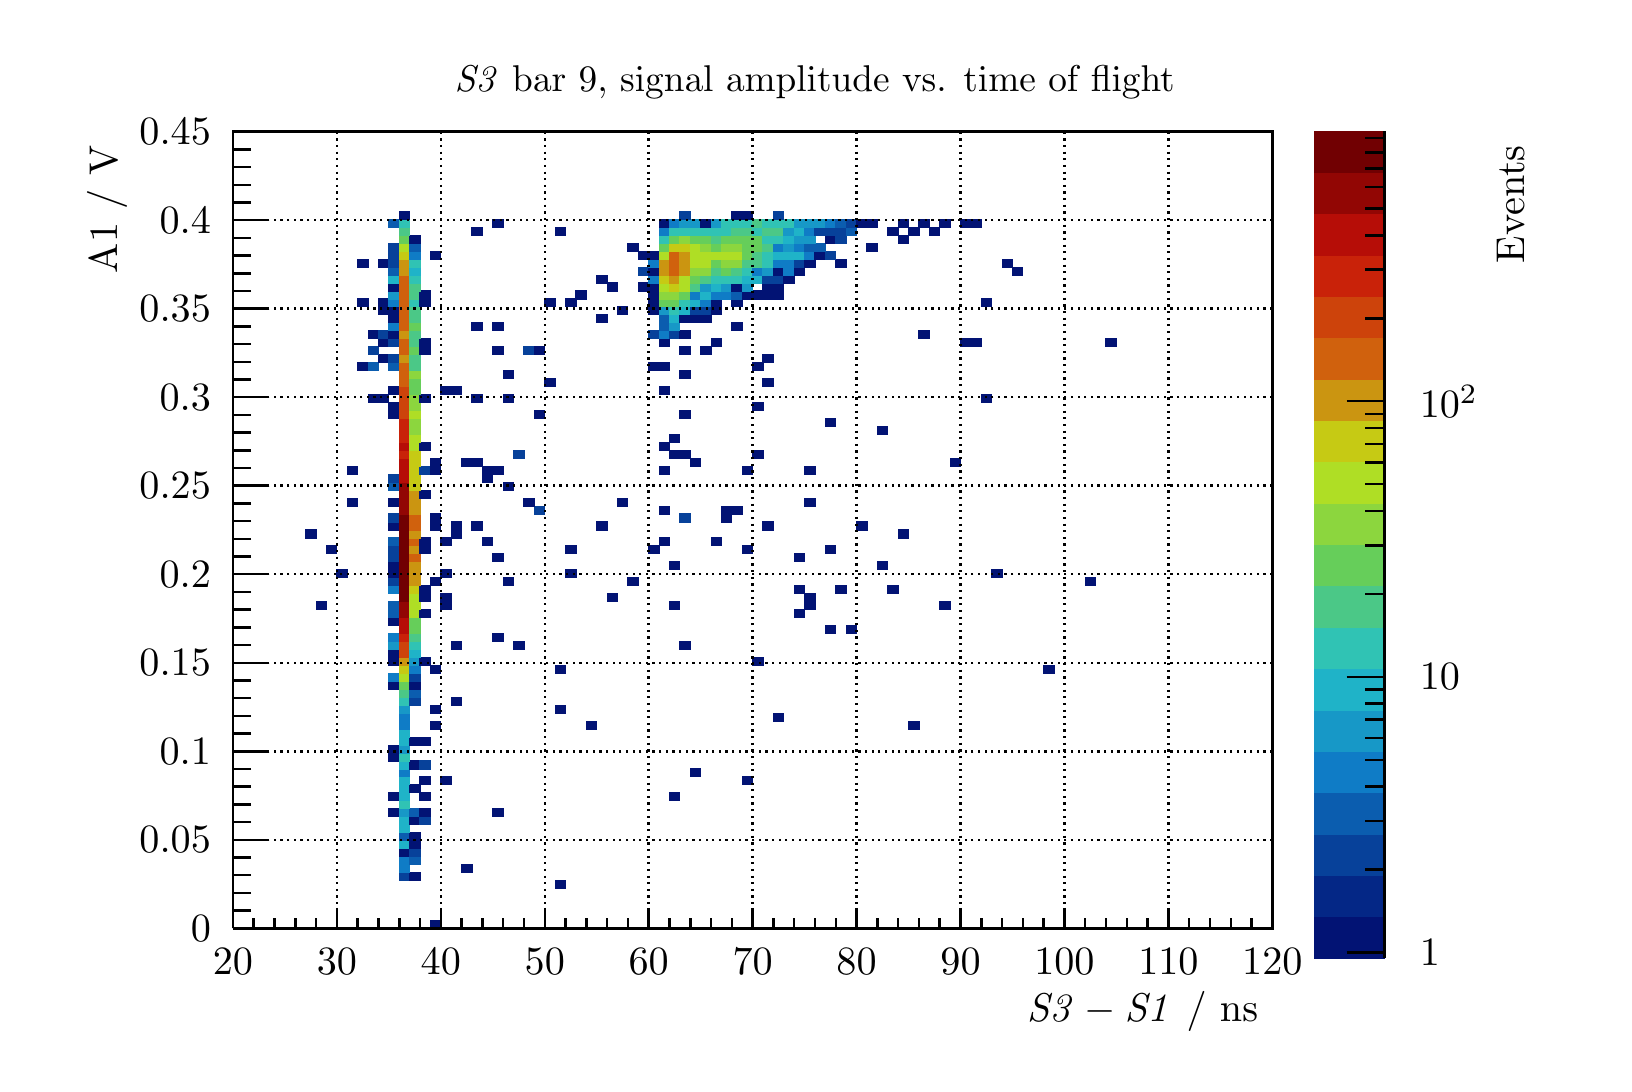
\begin{tikzpicture}
\pgfdeclareplotmark{cross} {
\pgfpathmoveto{\pgfpoint{-0.3\pgfplotmarksize}{\pgfplotmarksize}}
\pgfpathlineto{\pgfpoint{+0.3\pgfplotmarksize}{\pgfplotmarksize}}
\pgfpathlineto{\pgfpoint{+0.3\pgfplotmarksize}{0.3\pgfplotmarksize}}
\pgfpathlineto{\pgfpoint{+1\pgfplotmarksize}{0.3\pgfplotmarksize}}
\pgfpathlineto{\pgfpoint{+1\pgfplotmarksize}{-0.3\pgfplotmarksize}}
\pgfpathlineto{\pgfpoint{+0.3\pgfplotmarksize}{-0.3\pgfplotmarksize}}
\pgfpathlineto{\pgfpoint{+0.3\pgfplotmarksize}{-1.\pgfplotmarksize}}
\pgfpathlineto{\pgfpoint{-0.3\pgfplotmarksize}{-1.\pgfplotmarksize}}
\pgfpathlineto{\pgfpoint{-0.3\pgfplotmarksize}{-0.3\pgfplotmarksize}}
\pgfpathlineto{\pgfpoint{-1.\pgfplotmarksize}{-0.3\pgfplotmarksize}}
\pgfpathlineto{\pgfpoint{-1.\pgfplotmarksize}{0.3\pgfplotmarksize}}
\pgfpathlineto{\pgfpoint{-0.3\pgfplotmarksize}{0.3\pgfplotmarksize}}
\pgfpathclose
\pgfusepathqstroke
}
\pgfdeclareplotmark{cross*} {
\pgfpathmoveto{\pgfpoint{-0.3\pgfplotmarksize}{\pgfplotmarksize}}
\pgfpathlineto{\pgfpoint{+0.3\pgfplotmarksize}{\pgfplotmarksize}}
\pgfpathlineto{\pgfpoint{+0.3\pgfplotmarksize}{0.3\pgfplotmarksize}}
\pgfpathlineto{\pgfpoint{+1\pgfplotmarksize}{0.3\pgfplotmarksize}}
\pgfpathlineto{\pgfpoint{+1\pgfplotmarksize}{-0.3\pgfplotmarksize}}
\pgfpathlineto{\pgfpoint{+0.3\pgfplotmarksize}{-0.3\pgfplotmarksize}}
\pgfpathlineto{\pgfpoint{+0.3\pgfplotmarksize}{-1.\pgfplotmarksize}}
\pgfpathlineto{\pgfpoint{-0.3\pgfplotmarksize}{-1.\pgfplotmarksize}}
\pgfpathlineto{\pgfpoint{-0.3\pgfplotmarksize}{-0.3\pgfplotmarksize}}
\pgfpathlineto{\pgfpoint{-1.\pgfplotmarksize}{-0.3\pgfplotmarksize}}
\pgfpathlineto{\pgfpoint{-1.\pgfplotmarksize}{0.3\pgfplotmarksize}}
\pgfpathlineto{\pgfpoint{-0.3\pgfplotmarksize}{0.3\pgfplotmarksize}}
\pgfpathclose
\pgfusepathqfillstroke
}
\pgfdeclareplotmark{newstar} {
\pgfpathmoveto{\pgfqpoint{0pt}{\pgfplotmarksize}}
\pgfpathlineto{\pgfqpointpolar{44}{0.5\pgfplotmarksize}}
\pgfpathlineto{\pgfqpointpolar{18}{\pgfplotmarksize}}
\pgfpathlineto{\pgfqpointpolar{-20}{0.5\pgfplotmarksize}}
\pgfpathlineto{\pgfqpointpolar{-54}{\pgfplotmarksize}}
\pgfpathlineto{\pgfqpointpolar{-90}{0.5\pgfplotmarksize}}
\pgfpathlineto{\pgfqpointpolar{234}{\pgfplotmarksize}}
\pgfpathlineto{\pgfqpointpolar{198}{0.5\pgfplotmarksize}}
\pgfpathlineto{\pgfqpointpolar{162}{\pgfplotmarksize}}
\pgfpathlineto{\pgfqpointpolar{134}{0.5\pgfplotmarksize}}
\pgfpathclose
\pgfusepathqstroke
}
\pgfdeclareplotmark{newstar*} {
\pgfpathmoveto{\pgfqpoint{0pt}{\pgfplotmarksize}}
\pgfpathlineto{\pgfqpointpolar{44}{0.5\pgfplotmarksize}}
\pgfpathlineto{\pgfqpointpolar{18}{\pgfplotmarksize}}
\pgfpathlineto{\pgfqpointpolar{-20}{0.5\pgfplotmarksize}}
\pgfpathlineto{\pgfqpointpolar{-54}{\pgfplotmarksize}}
\pgfpathlineto{\pgfqpointpolar{-90}{0.5\pgfplotmarksize}}
\pgfpathlineto{\pgfqpointpolar{234}{\pgfplotmarksize}}
\pgfpathlineto{\pgfqpointpolar{198}{0.5\pgfplotmarksize}}
\pgfpathlineto{\pgfqpointpolar{162}{\pgfplotmarksize}}
\pgfpathlineto{\pgfqpointpolar{134}{0.5\pgfplotmarksize}}
\pgfpathclose
\pgfusepathqfillstroke
}
\definecolor{c}{rgb}{1,1,1};
\draw [color=c, fill=c] (0,0) rectangle (20,13.1389);
\draw [color=c, fill=c] (2.6,1.70805) rectangle (15.8,11.825);
\definecolor{c}{rgb}{0,0,0};
\draw [c,line width=0.9] (2.6,1.70805) -- (2.6,11.825) -- (15.8,11.825) -- (15.8,1.70805) -- (2.6,1.70805);
\definecolor{c}{rgb}{1,1,1};
\draw [color=c, fill=c] (2.6,1.70805) rectangle (15.8,11.825);
\definecolor{c}{rgb}{0,0,0};
\draw [c,line width=0.9] (2.6,1.70805) -- (2.6,11.825) -- (15.8,11.825) -- (15.8,1.70805) -- (2.6,1.70805);
\definecolor{c}{rgb}{0.00759013,0.0728653,0.45351};
\draw [color=c, fill=c] (5.108,1.70805) rectangle (5.24,1.80922);
\draw [color=c, fill=c] (6.692,2.2139) rectangle (6.824,2.31507);
\definecolor{c}{rgb}{0.0281863,0.253431,0.604902};
\draw [color=c, fill=c] (4.712,2.31507) rectangle (4.844,2.41624);
\definecolor{c}{rgb}{0.00759013,0.0728653,0.45351};
\draw [color=c, fill=c] (4.844,2.31507) rectangle (4.976,2.41624);
\definecolor{c}{rgb}{0.0588235,0.486275,0.776471};
\draw [color=c, fill=c] (4.712,2.41624) rectangle (4.844,2.51741);
\definecolor{c}{rgb}{0.00759013,0.0728653,0.45351};
\draw [color=c, fill=c] (5.504,2.41624) rectangle (5.636,2.51741);
\definecolor{c}{rgb}{0.0588235,0.486275,0.776471};
\draw [color=c, fill=c] (4.712,2.51741) rectangle (4.844,2.61857);
\definecolor{c}{rgb}{0.0428922,0.365196,0.687255};
\draw [color=c, fill=c] (4.844,2.51741) rectangle (4.976,2.61857);
\definecolor{c}{rgb}{0.00759013,0.0728653,0.45351};
\draw [color=c, fill=c] (4.712,2.61857) rectangle (4.844,2.71974);
\definecolor{c}{rgb}{0.0281863,0.253431,0.604902};
\draw [color=c, fill=c] (4.844,2.61857) rectangle (4.976,2.71974);
\definecolor{c}{rgb}{0.122549,0.702941,0.786029};
\draw [color=c, fill=c] (4.712,2.71974) rectangle (4.844,2.82091);
\definecolor{c}{rgb}{0.00759013,0.0728653,0.45351};
\draw [color=c, fill=c] (4.844,2.71974) rectangle (4.976,2.82091);
\definecolor{c}{rgb}{0.0428922,0.365196,0.687255};
\draw [color=c, fill=c] (4.712,2.82091) rectangle (4.844,2.92208);
\definecolor{c}{rgb}{0.00759013,0.0728653,0.45351};
\draw [color=c, fill=c] (4.844,2.82091) rectangle (4.976,2.92208);
\definecolor{c}{rgb}{0.122549,0.702941,0.786029};
\draw [color=c, fill=c] (4.712,2.92208) rectangle (4.844,3.02325);
\draw [color=c, fill=c] (4.712,3.02325) rectangle (4.844,3.12442);
\definecolor{c}{rgb}{0.00759013,0.0728653,0.45351};
\draw [color=c, fill=c] (4.844,3.02325) rectangle (4.976,3.12442);
\definecolor{c}{rgb}{0.0281863,0.253431,0.604902};
\draw [color=c, fill=c] (4.976,3.02325) rectangle (5.108,3.12442);
\definecolor{c}{rgb}{0.00759013,0.0728653,0.45351};
\draw [color=c, fill=c] (4.58,3.12442) rectangle (4.712,3.22559);
\definecolor{c}{rgb}{0.0906863,0.594608,0.78125};
\draw [color=c, fill=c] (4.712,3.12442) rectangle (4.844,3.22559);
\definecolor{c}{rgb}{0.0428922,0.365196,0.687255};
\draw [color=c, fill=c] (4.844,3.12442) rectangle (4.976,3.22559);
\definecolor{c}{rgb}{0.00759013,0.0728653,0.45351};
\draw [color=c, fill=c] (4.976,3.12442) rectangle (5.108,3.22559);
\draw [color=c, fill=c] (5.9,3.12442) rectangle (6.032,3.22559);
\definecolor{c}{rgb}{0.18652,0.763235,0.706618};
\draw [color=c, fill=c] (4.712,3.22559) rectangle (4.844,3.32676);
\definecolor{c}{rgb}{0.00759013,0.0728653,0.45351};
\draw [color=c, fill=c] (4.58,3.32676) rectangle (4.712,3.42793);
\definecolor{c}{rgb}{0.122549,0.702941,0.786029};
\draw [color=c, fill=c] (4.712,3.32676) rectangle (4.844,3.42793);
\definecolor{c}{rgb}{0.00759013,0.0728653,0.45351};
\draw [color=c, fill=c] (4.976,3.32676) rectangle (5.108,3.42793);
\draw [color=c, fill=c] (8.144,3.32676) rectangle (8.276,3.42793);
\definecolor{c}{rgb}{0.122549,0.702941,0.786029};
\draw [color=c, fill=c] (4.712,3.42793) rectangle (4.844,3.5291);
\definecolor{c}{rgb}{0.00759013,0.0728653,0.45351};
\draw [color=c, fill=c] (4.844,3.42793) rectangle (4.976,3.5291);
\definecolor{c}{rgb}{0.122549,0.702941,0.786029};
\draw [color=c, fill=c] (4.712,3.5291) rectangle (4.844,3.63027);
\definecolor{c}{rgb}{0.00759013,0.0728653,0.45351};
\draw [color=c, fill=c] (4.976,3.5291) rectangle (5.108,3.63027);
\draw [color=c, fill=c] (5.24,3.5291) rectangle (5.372,3.63027);
\draw [color=c, fill=c] (9.068,3.5291) rectangle (9.2,3.63027);
\definecolor{c}{rgb}{0.0588235,0.486275,0.776471};
\draw [color=c, fill=c] (4.712,3.63027) rectangle (4.844,3.73144);
\definecolor{c}{rgb}{0.00759013,0.0728653,0.45351};
\draw [color=c, fill=c] (8.408,3.63027) rectangle (8.54,3.73144);
\definecolor{c}{rgb}{0.122549,0.702941,0.786029};
\draw [color=c, fill=c] (4.712,3.73144) rectangle (4.844,3.8326);
\definecolor{c}{rgb}{0.00759013,0.0728653,0.45351};
\draw [color=c, fill=c] (4.844,3.73144) rectangle (4.976,3.8326);
\definecolor{c}{rgb}{0.0281863,0.253431,0.604902};
\draw [color=c, fill=c] (4.976,3.73144) rectangle (5.108,3.8326);
\definecolor{c}{rgb}{0.00759013,0.0728653,0.45351};
\draw [color=c, fill=c] (4.58,3.8326) rectangle (4.712,3.93377);
\definecolor{c}{rgb}{0.18652,0.763235,0.706618};
\draw [color=c, fill=c] (4.712,3.8326) rectangle (4.844,3.93377);
\definecolor{c}{rgb}{0.00759013,0.0728653,0.45351};
\draw [color=c, fill=c] (4.58,3.93377) rectangle (4.712,4.03494);
\definecolor{c}{rgb}{0.0906863,0.594608,0.78125};
\draw [color=c, fill=c] (4.712,3.93377) rectangle (4.844,4.03494);
\definecolor{c}{rgb}{0.122549,0.702941,0.786029};
\draw [color=c, fill=c] (4.712,4.03494) rectangle (4.844,4.13611);
\definecolor{c}{rgb}{0.00759013,0.0728653,0.45351};
\draw [color=c, fill=c] (4.844,4.03494) rectangle (4.976,4.13611);
\draw [color=c, fill=c] (4.976,4.03494) rectangle (5.108,4.13611);
\definecolor{c}{rgb}{0.122549,0.702941,0.786029};
\draw [color=c, fill=c] (4.712,4.13611) rectangle (4.844,4.23728);
\definecolor{c}{rgb}{0.0588235,0.486275,0.776471};
\draw [color=c, fill=c] (4.712,4.23728) rectangle (4.844,4.33845);
\definecolor{c}{rgb}{0.00759013,0.0728653,0.45351};
\draw [color=c, fill=c] (5.108,4.23728) rectangle (5.24,4.33845);
\draw [color=c, fill=c] (7.088,4.23728) rectangle (7.22,4.33845);
\draw [color=c, fill=c] (11.18,4.23728) rectangle (11.312,4.33845);
\definecolor{c}{rgb}{0.0588235,0.486275,0.776471};
\draw [color=c, fill=c] (4.712,4.33845) rectangle (4.844,4.43962);
\definecolor{c}{rgb}{0.00759013,0.0728653,0.45351};
\draw [color=c, fill=c] (9.464,4.33845) rectangle (9.596,4.43962);
\definecolor{c}{rgb}{0.0906863,0.594608,0.78125};
\draw [color=c, fill=c] (4.712,4.43962) rectangle (4.844,4.54079);
\definecolor{c}{rgb}{0.00759013,0.0728653,0.45351};
\draw [color=c, fill=c] (5.108,4.43962) rectangle (5.24,4.54079);
\draw [color=c, fill=c] (6.692,4.43962) rectangle (6.824,4.54079);
\definecolor{c}{rgb}{0.18652,0.763235,0.706618};
\draw [color=c, fill=c] (4.712,4.54079) rectangle (4.844,4.64196);
\definecolor{c}{rgb}{0.0281863,0.253431,0.604902};
\draw [color=c, fill=c] (4.844,4.54079) rectangle (4.976,4.64196);
\definecolor{c}{rgb}{0.00759013,0.0728653,0.45351};
\draw [color=c, fill=c] (5.372,4.54079) rectangle (5.504,4.64196);
\definecolor{c}{rgb}{0.29326,0.785539,0.529779};
\draw [color=c, fill=c] (4.712,4.64196) rectangle (4.844,4.74313);
\definecolor{c}{rgb}{0.0428922,0.365196,0.687255};
\draw [color=c, fill=c] (4.844,4.64196) rectangle (4.976,4.74313);
\definecolor{c}{rgb}{0.00759013,0.0728653,0.45351};
\draw [color=c, fill=c] (4.58,4.74313) rectangle (4.712,4.8443);
\definecolor{c}{rgb}{0.4,0.807843,0.352941};
\draw [color=c, fill=c] (4.712,4.74313) rectangle (4.844,4.8443);
\definecolor{c}{rgb}{0.00759013,0.0728653,0.45351};
\draw [color=c, fill=c] (4.844,4.74313) rectangle (4.976,4.8443);
\definecolor{c}{rgb}{0.0588235,0.486275,0.776471};
\draw [color=c, fill=c] (4.58,4.8443) rectangle (4.712,4.94547);
\definecolor{c}{rgb}{0.68799,0.869118,0.144608};
\draw [color=c, fill=c] (4.712,4.8443) rectangle (4.844,4.94547);
\definecolor{c}{rgb}{0.0281863,0.253431,0.604902};
\draw [color=c, fill=c] (4.844,4.8443) rectangle (4.976,4.94547);
\definecolor{c}{rgb}{0.777451,0.791422,0.0796569};
\draw [color=c, fill=c] (4.712,4.94547) rectangle (4.844,5.04663);
\definecolor{c}{rgb}{0.0588235,0.486275,0.776471};
\draw [color=c, fill=c] (4.844,4.94547) rectangle (4.976,5.04663);
\definecolor{c}{rgb}{0.00759013,0.0728653,0.45351};
\draw [color=c, fill=c] (5.108,4.94547) rectangle (5.24,5.04663);
\draw [color=c, fill=c] (6.692,4.94547) rectangle (6.824,5.04663);
\draw [color=c, fill=c] (12.896,4.94547) rectangle (13.028,5.04663);
\draw [color=c, fill=c] (4.58,5.04663) rectangle (4.712,5.1478);
\definecolor{c}{rgb}{0.796569,0.585907,0.0653186};
\draw [color=c, fill=c] (4.712,5.04663) rectangle (4.844,5.1478);
\definecolor{c}{rgb}{0.0906863,0.594608,0.78125};
\draw [color=c, fill=c] (4.844,5.04663) rectangle (4.976,5.1478);
\definecolor{c}{rgb}{0.00759013,0.0728653,0.45351};
\draw [color=c, fill=c] (4.976,5.04663) rectangle (5.108,5.1478);
\draw [color=c, fill=c] (9.2,5.04663) rectangle (9.332,5.1478);
\draw [color=c, fill=c] (4.58,5.1478) rectangle (4.712,5.24897);
\definecolor{c}{rgb}{0.802451,0.261275,0.0436275};
\draw [color=c, fill=c] (4.712,5.1478) rectangle (4.844,5.24897);
\definecolor{c}{rgb}{0.122549,0.702941,0.786029};
\draw [color=c, fill=c] (4.844,5.1478) rectangle (4.976,5.24897);
\definecolor{c}{rgb}{0.0906863,0.594608,0.78125};
\draw [color=c, fill=c] (4.58,5.24897) rectangle (4.712,5.35014);
\definecolor{c}{rgb}{0.802451,0.261275,0.0436275};
\draw [color=c, fill=c] (4.712,5.24897) rectangle (4.844,5.35014);
\definecolor{c}{rgb}{0.18652,0.763235,0.706618};
\draw [color=c, fill=c] (4.844,5.24897) rectangle (4.976,5.35014);
\definecolor{c}{rgb}{0.00759013,0.0728653,0.45351};
\draw [color=c, fill=c] (5.372,5.24897) rectangle (5.504,5.35014);
\draw [color=c, fill=c] (6.164,5.24897) rectangle (6.296,5.35014);
\draw [color=c, fill=c] (8.276,5.24897) rectangle (8.408,5.35014);
\definecolor{c}{rgb}{0.0588235,0.486275,0.776471};
\draw [color=c, fill=c] (4.58,5.35014) rectangle (4.712,5.45131);
\definecolor{c}{rgb}{0.788113,0.13223,0.0356618};
\draw [color=c, fill=c] (4.712,5.35014) rectangle (4.844,5.45131);
\definecolor{c}{rgb}{0.29326,0.785539,0.529779};
\draw [color=c, fill=c] (4.844,5.35014) rectangle (4.976,5.45131);
\definecolor{c}{rgb}{0.00759013,0.0728653,0.45351};
\draw [color=c, fill=c] (5.9,5.35014) rectangle (6.032,5.45131);
\definecolor{c}{rgb}{0.714951,0.0509804,0.0269608};
\draw [color=c, fill=c] (4.712,5.45131) rectangle (4.844,5.55248);
\definecolor{c}{rgb}{0.4,0.807843,0.352941};
\draw [color=c, fill=c] (4.844,5.45131) rectangle (4.976,5.55248);
\definecolor{c}{rgb}{0.00759013,0.0728653,0.45351};
\draw [color=c, fill=c] (10.124,5.45131) rectangle (10.256,5.55248);
\draw [color=c, fill=c] (10.388,5.45131) rectangle (10.52,5.55248);
\draw [color=c, fill=c] (4.58,5.55248) rectangle (4.712,5.65365);
\definecolor{c}{rgb}{0.714951,0.0509804,0.0269608};
\draw [color=c, fill=c] (4.712,5.55248) rectangle (4.844,5.65365);
\definecolor{c}{rgb}{0.4,0.807843,0.352941};
\draw [color=c, fill=c] (4.844,5.55248) rectangle (4.976,5.65365);
\definecolor{c}{rgb}{0.0428922,0.365196,0.687255};
\draw [color=c, fill=c] (4.58,5.65365) rectangle (4.712,5.75482);
\definecolor{c}{rgb}{0.573162,0.0254902,0.017402};
\draw [color=c, fill=c] (4.712,5.65365) rectangle (4.844,5.75482);
\definecolor{c}{rgb}{0.68799,0.869118,0.144608};
\draw [color=c, fill=c] (4.844,5.65365) rectangle (4.976,5.75482);
\definecolor{c}{rgb}{0.00759013,0.0728653,0.45351};
\draw [color=c, fill=c] (4.976,5.65365) rectangle (5.108,5.75482);
\draw [color=c, fill=c] (9.728,5.65365) rectangle (9.86,5.75482);
\draw [color=c, fill=c] (3.656,5.75482) rectangle (3.788,5.85599);
\definecolor{c}{rgb}{0.0428922,0.365196,0.687255};
\draw [color=c, fill=c] (4.58,5.75482) rectangle (4.712,5.85599);
\definecolor{c}{rgb}{0.573162,0.0254902,0.017402};
\draw [color=c, fill=c] (4.712,5.75482) rectangle (4.844,5.85599);
\definecolor{c}{rgb}{0.68799,0.869118,0.144608};
\draw [color=c, fill=c] (4.844,5.75482) rectangle (4.976,5.85599);
\definecolor{c}{rgb}{0.00759013,0.0728653,0.45351};
\draw [color=c, fill=c] (5.24,5.75482) rectangle (5.372,5.85599);
\draw [color=c, fill=c] (8.144,5.75482) rectangle (8.276,5.85599);
\draw [color=c, fill=c] (9.86,5.75482) rectangle (9.992,5.85599);
\draw [color=c, fill=c] (11.576,5.75482) rectangle (11.708,5.85599);
\definecolor{c}{rgb}{0.442279,0.00196078,0.00857843};
\draw [color=c, fill=c] (4.712,5.85599) rectangle (4.844,5.95716);
\definecolor{c}{rgb}{0.68799,0.869118,0.144608};
\draw [color=c, fill=c] (4.844,5.85599) rectangle (4.976,5.95716);
\definecolor{c}{rgb}{0.00759013,0.0728653,0.45351};
\draw [color=c, fill=c] (4.976,5.85599) rectangle (5.108,5.95716);
\draw [color=c, fill=c] (5.24,5.85599) rectangle (5.372,5.95716);
\draw [color=c, fill=c] (7.352,5.85599) rectangle (7.484,5.95716);
\draw [color=c, fill=c] (9.86,5.85599) rectangle (9.992,5.95716);
\definecolor{c}{rgb}{0.0588235,0.486275,0.776471};
\draw [color=c, fill=c] (4.58,5.95716) rectangle (4.712,6.05833);
\definecolor{c}{rgb}{0.442279,0.00196078,0.00857843};
\draw [color=c, fill=c] (4.712,5.95716) rectangle (4.844,6.05833);
\definecolor{c}{rgb}{0.777451,0.791422,0.0796569};
\draw [color=c, fill=c] (4.844,5.95716) rectangle (4.976,6.05833);
\definecolor{c}{rgb}{0.00759013,0.0728653,0.45351};
\draw [color=c, fill=c] (4.976,5.95716) rectangle (5.108,6.05833);
\draw [color=c, fill=c] (9.728,5.95716) rectangle (9.86,6.05833);
\draw [color=c, fill=c] (10.256,5.95716) rectangle (10.388,6.05833);
\draw [color=c, fill=c] (10.916,5.95716) rectangle (11.048,6.05833);
\definecolor{c}{rgb}{0.0281863,0.253431,0.604902};
\draw [color=c, fill=c] (4.58,6.05833) rectangle (4.712,6.1595);
\definecolor{c}{rgb}{0.442279,0.00196078,0.00857843};
\draw [color=c, fill=c] (4.712,6.05833) rectangle (4.844,6.1595);
\definecolor{c}{rgb}{0.796569,0.585907,0.0653186};
\draw [color=c, fill=c] (4.844,6.05833) rectangle (4.976,6.1595);
\definecolor{c}{rgb}{0.00759013,0.0728653,0.45351};
\draw [color=c, fill=c] (5.108,6.05833) rectangle (5.24,6.1595);
\draw [color=c, fill=c] (6.032,6.05833) rectangle (6.164,6.1595);
\draw [color=c, fill=c] (7.616,6.05833) rectangle (7.748,6.1595);
\draw [color=c, fill=c] (13.424,6.05833) rectangle (13.556,6.1595);
\draw [color=c, fill=c] (3.92,6.1595) rectangle (4.052,6.26067);
\draw [color=c, fill=c] (4.58,6.1595) rectangle (4.712,6.26067);
\definecolor{c}{rgb}{0.442279,0.00196078,0.00857843};
\draw [color=c, fill=c] (4.712,6.1595) rectangle (4.844,6.26067);
\definecolor{c}{rgb}{0.796569,0.585907,0.0653186};
\draw [color=c, fill=c] (4.844,6.1595) rectangle (4.976,6.26067);
\definecolor{c}{rgb}{0.00759013,0.0728653,0.45351};
\draw [color=c, fill=c] (5.24,6.1595) rectangle (5.372,6.26067);
\draw [color=c, fill=c] (6.824,6.1595) rectangle (6.956,6.26067);
\draw [color=c, fill=c] (12.236,6.1595) rectangle (12.368,6.26067);
\draw [color=c, fill=c] (4.58,6.26067) rectangle (4.712,6.36183);
\definecolor{c}{rgb}{0.442279,0.00196078,0.00857843};
\draw [color=c, fill=c] (4.712,6.26067) rectangle (4.844,6.36183);
\definecolor{c}{rgb}{0.796569,0.585907,0.0653186};
\draw [color=c, fill=c] (4.844,6.26067) rectangle (4.976,6.36183);
\definecolor{c}{rgb}{0.00759013,0.0728653,0.45351};
\draw [color=c, fill=c] (8.144,6.26067) rectangle (8.276,6.36183);
\draw [color=c, fill=c] (10.784,6.26067) rectangle (10.916,6.36183);
\definecolor{c}{rgb}{0.0281863,0.253431,0.604902};
\draw [color=c, fill=c] (4.58,6.36183) rectangle (4.712,6.463);
\definecolor{c}{rgb}{0.442279,0.00196078,0.00857843};
\draw [color=c, fill=c] (4.712,6.36183) rectangle (4.844,6.463);
\definecolor{c}{rgb}{0.815686,0.380392,0.0509804};
\draw [color=c, fill=c] (4.844,6.36183) rectangle (4.976,6.463);
\definecolor{c}{rgb}{0.00759013,0.0728653,0.45351};
\draw [color=c, fill=c] (5.9,6.36183) rectangle (6.032,6.463);
\draw [color=c, fill=c] (9.728,6.36183) rectangle (9.86,6.463);
\draw [color=c, fill=c] (3.788,6.463) rectangle (3.92,6.56417);
\definecolor{c}{rgb}{0.0281863,0.253431,0.604902};
\draw [color=c, fill=c] (4.58,6.463) rectangle (4.712,6.56417);
\definecolor{c}{rgb}{0.442279,0.00196078,0.00857843};
\draw [color=c, fill=c] (4.712,6.463) rectangle (4.844,6.56417);
\definecolor{c}{rgb}{0.796569,0.585907,0.0653186};
\draw [color=c, fill=c] (4.844,6.463) rectangle (4.976,6.56417);
\definecolor{c}{rgb}{0.00759013,0.0728653,0.45351};
\draw [color=c, fill=c] (4.976,6.463) rectangle (5.108,6.56417);
\draw [color=c, fill=c] (6.824,6.463) rectangle (6.956,6.56417);
\draw [color=c, fill=c] (7.88,6.463) rectangle (8.012,6.56417);
\draw [color=c, fill=c] (9.068,6.463) rectangle (9.2,6.56417);
\draw [color=c, fill=c] (10.124,6.463) rectangle (10.256,6.56417);
\definecolor{c}{rgb}{0.0428922,0.365196,0.687255};
\draw [color=c, fill=c] (4.58,6.56417) rectangle (4.712,6.66534);
\definecolor{c}{rgb}{0.442279,0.00196078,0.00857843};
\draw [color=c, fill=c] (4.712,6.56417) rectangle (4.844,6.66534);
\definecolor{c}{rgb}{0.815686,0.380392,0.0509804};
\draw [color=c, fill=c] (4.844,6.56417) rectangle (4.976,6.66534);
\definecolor{c}{rgb}{0.00759013,0.0728653,0.45351};
\draw [color=c, fill=c] (4.976,6.56417) rectangle (5.108,6.66534);
\draw [color=c, fill=c] (5.24,6.56417) rectangle (5.372,6.66534);
\draw [color=c, fill=c] (5.768,6.56417) rectangle (5.9,6.66534);
\draw [color=c, fill=c] (8.012,6.56417) rectangle (8.144,6.66534);
\draw [color=c, fill=c] (8.672,6.56417) rectangle (8.804,6.66534);
\draw [color=c, fill=c] (3.524,6.66534) rectangle (3.656,6.76651);
\definecolor{c}{rgb}{0.442279,0.00196078,0.00857843};
\draw [color=c, fill=c] (4.712,6.66534) rectangle (4.844,6.76651);
\definecolor{c}{rgb}{0.796569,0.585907,0.0653186};
\draw [color=c, fill=c] (4.844,6.66534) rectangle (4.976,6.76651);
\definecolor{c}{rgb}{0.00759013,0.0728653,0.45351};
\draw [color=c, fill=c] (5.372,6.66534) rectangle (5.504,6.76651);
\draw [color=c, fill=c] (11.048,6.66534) rectangle (11.18,6.76651);
\draw [color=c, fill=c] (4.58,6.76651) rectangle (4.712,6.86768);
\definecolor{c}{rgb}{0.442279,0.00196078,0.00857843};
\draw [color=c, fill=c] (4.712,6.76651) rectangle (4.844,6.86768);
\definecolor{c}{rgb}{0.815686,0.380392,0.0509804};
\draw [color=c, fill=c] (4.844,6.76651) rectangle (4.976,6.86768);
\definecolor{c}{rgb}{0.00759013,0.0728653,0.45351};
\draw [color=c, fill=c] (5.108,6.76651) rectangle (5.24,6.86768);
\draw [color=c, fill=c] (5.372,6.76651) rectangle (5.504,6.86768);
\draw [color=c, fill=c] (5.636,6.76651) rectangle (5.768,6.86768);
\draw [color=c, fill=c] (7.22,6.76651) rectangle (7.352,6.86768);
\draw [color=c, fill=c] (9.332,6.76651) rectangle (9.464,6.86768);
\draw [color=c, fill=c] (10.52,6.76651) rectangle (10.652,6.86768);
\definecolor{c}{rgb}{0.0281863,0.253431,0.604902};
\draw [color=c, fill=c] (4.58,6.86768) rectangle (4.712,6.96885);
\definecolor{c}{rgb}{0.442279,0.00196078,0.00857843};
\draw [color=c, fill=c] (4.712,6.86768) rectangle (4.844,6.96885);
\definecolor{c}{rgb}{0.815686,0.380392,0.0509804};
\draw [color=c, fill=c] (4.844,6.86768) rectangle (4.976,6.96885);
\definecolor{c}{rgb}{0.00759013,0.0728653,0.45351};
\draw [color=c, fill=c] (5.108,6.86768) rectangle (5.24,6.96885);
\definecolor{c}{rgb}{0.0281863,0.253431,0.604902};
\draw [color=c, fill=c] (8.276,6.86768) rectangle (8.408,6.96885);
\definecolor{c}{rgb}{0.00759013,0.0728653,0.45351};
\draw [color=c, fill=c] (8.804,6.86768) rectangle (8.936,6.96885);
\definecolor{c}{rgb}{0.573162,0.0254902,0.017402};
\draw [color=c, fill=c] (4.712,6.96885) rectangle (4.844,7.07002);
\definecolor{c}{rgb}{0.796569,0.585907,0.0653186};
\draw [color=c, fill=c] (4.844,6.96885) rectangle (4.976,7.07002);
\definecolor{c}{rgb}{0.0281863,0.253431,0.604902};
\draw [color=c, fill=c] (6.428,6.96885) rectangle (6.56,7.07002);
\definecolor{c}{rgb}{0.00759013,0.0728653,0.45351};
\draw [color=c, fill=c] (8.012,6.96885) rectangle (8.144,7.07002);
\draw [color=c, fill=c] (8.804,6.96885) rectangle (8.936,7.07002);
\draw [color=c, fill=c] (8.936,6.96885) rectangle (9.068,7.07002);
\draw [color=c, fill=c] (4.052,7.07002) rectangle (4.184,7.17119);
\draw [color=c, fill=c] (4.58,7.07002) rectangle (4.712,7.17119);
\definecolor{c}{rgb}{0.573162,0.0254902,0.017402};
\draw [color=c, fill=c] (4.712,7.07002) rectangle (4.844,7.17119);
\definecolor{c}{rgb}{0.796569,0.585907,0.0653186};
\draw [color=c, fill=c] (4.844,7.07002) rectangle (4.976,7.17119);
\definecolor{c}{rgb}{0.00759013,0.0728653,0.45351};
\draw [color=c, fill=c] (6.296,7.07002) rectangle (6.428,7.17119);
\draw [color=c, fill=c] (7.484,7.07002) rectangle (7.616,7.17119);
\draw [color=c, fill=c] (9.86,7.07002) rectangle (9.992,7.17119);
\definecolor{c}{rgb}{0.573162,0.0254902,0.017402};
\draw [color=c, fill=c] (4.712,7.17119) rectangle (4.844,7.27236);
\definecolor{c}{rgb}{0.796569,0.585907,0.0653186};
\draw [color=c, fill=c] (4.844,7.17119) rectangle (4.976,7.27236);
\definecolor{c}{rgb}{0.00759013,0.0728653,0.45351};
\draw [color=c, fill=c] (4.976,7.17119) rectangle (5.108,7.27236);
\definecolor{c}{rgb}{0.0428922,0.365196,0.687255};
\draw [color=c, fill=c] (4.58,7.27236) rectangle (4.712,7.37353);
\definecolor{c}{rgb}{0.573162,0.0254902,0.017402};
\draw [color=c, fill=c] (4.712,7.27236) rectangle (4.844,7.37353);
\definecolor{c}{rgb}{0.777451,0.791422,0.0796569};
\draw [color=c, fill=c] (4.844,7.27236) rectangle (4.976,7.37353);
\definecolor{c}{rgb}{0.00759013,0.0728653,0.45351};
\draw [color=c, fill=c] (6.032,7.27236) rectangle (6.164,7.37353);
\definecolor{c}{rgb}{0.0281863,0.253431,0.604902};
\draw [color=c, fill=c] (4.58,7.37353) rectangle (4.712,7.4747);
\definecolor{c}{rgb}{0.714951,0.0509804,0.0269608};
\draw [color=c, fill=c] (4.712,7.37353) rectangle (4.844,7.4747);
\definecolor{c}{rgb}{0.777451,0.791422,0.0796569};
\draw [color=c, fill=c] (4.844,7.37353) rectangle (4.976,7.4747);
\definecolor{c}{rgb}{0.00759013,0.0728653,0.45351};
\draw [color=c, fill=c] (5.768,7.37353) rectangle (5.9,7.4747);
\draw [color=c, fill=c] (4.052,7.4747) rectangle (4.184,7.57586);
\definecolor{c}{rgb}{0.714951,0.0509804,0.0269608};
\draw [color=c, fill=c] (4.712,7.4747) rectangle (4.844,7.57586);
\definecolor{c}{rgb}{0.777451,0.791422,0.0796569};
\draw [color=c, fill=c] (4.844,7.4747) rectangle (4.976,7.57586);
\definecolor{c}{rgb}{0.0281863,0.253431,0.604902};
\draw [color=c, fill=c] (4.976,7.4747) rectangle (5.108,7.57586);
\definecolor{c}{rgb}{0.00759013,0.0728653,0.45351};
\draw [color=c, fill=c] (5.108,7.4747) rectangle (5.24,7.57586);
\draw [color=c, fill=c] (5.768,7.4747) rectangle (5.9,7.57586);
\draw [color=c, fill=c] (5.9,7.4747) rectangle (6.032,7.57586);
\draw [color=c, fill=c] (8.012,7.4747) rectangle (8.144,7.57586);
\draw [color=c, fill=c] (9.068,7.4747) rectangle (9.2,7.57586);
\draw [color=c, fill=c] (9.86,7.4747) rectangle (9.992,7.57586);
\definecolor{c}{rgb}{0.714951,0.0509804,0.0269608};
\draw [color=c, fill=c] (4.712,7.57586) rectangle (4.844,7.67703);
\definecolor{c}{rgb}{0.777451,0.791422,0.0796569};
\draw [color=c, fill=c] (4.844,7.57586) rectangle (4.976,7.67703);
\definecolor{c}{rgb}{0.00759013,0.0728653,0.45351};
\draw [color=c, fill=c] (5.108,7.57586) rectangle (5.24,7.67703);
\draw [color=c, fill=c] (5.504,7.57586) rectangle (5.636,7.67703);
\draw [color=c, fill=c] (5.636,7.57586) rectangle (5.768,7.67703);
\draw [color=c, fill=c] (8.408,7.57586) rectangle (8.54,7.67703);
\draw [color=c, fill=c] (11.708,7.57586) rectangle (11.84,7.67703);
\definecolor{c}{rgb}{0.788113,0.13223,0.0356618};
\draw [color=c, fill=c] (4.712,7.67703) rectangle (4.844,7.7782);
\definecolor{c}{rgb}{0.777451,0.791422,0.0796569};
\draw [color=c, fill=c] (4.844,7.67703) rectangle (4.976,7.7782);
\definecolor{c}{rgb}{0.0281863,0.253431,0.604902};
\draw [color=c, fill=c] (6.164,7.67703) rectangle (6.296,7.7782);
\definecolor{c}{rgb}{0.00759013,0.0728653,0.45351};
\draw [color=c, fill=c] (8.144,7.67703) rectangle (8.276,7.7782);
\draw [color=c, fill=c] (8.276,7.67703) rectangle (8.408,7.7782);
\draw [color=c, fill=c] (9.2,7.67703) rectangle (9.332,7.7782);
\definecolor{c}{rgb}{0.714951,0.0509804,0.0269608};
\draw [color=c, fill=c] (4.712,7.7782) rectangle (4.844,7.87937);
\definecolor{c}{rgb}{0.68799,0.869118,0.144608};
\draw [color=c, fill=c] (4.844,7.7782) rectangle (4.976,7.87937);
\definecolor{c}{rgb}{0.00759013,0.0728653,0.45351};
\draw [color=c, fill=c] (4.976,7.7782) rectangle (5.108,7.87937);
\draw [color=c, fill=c] (8.012,7.7782) rectangle (8.144,7.87937);
\definecolor{c}{rgb}{0.788113,0.13223,0.0356618};
\draw [color=c, fill=c] (4.712,7.87937) rectangle (4.844,7.98054);
\definecolor{c}{rgb}{0.68799,0.869118,0.144608};
\draw [color=c, fill=c] (4.844,7.87937) rectangle (4.976,7.98054);
\definecolor{c}{rgb}{0.00759013,0.0728653,0.45351};
\draw [color=c, fill=c] (8.144,7.87937) rectangle (8.276,7.98054);
\definecolor{c}{rgb}{0.788113,0.13223,0.0356618};
\draw [color=c, fill=c] (4.712,7.98054) rectangle (4.844,8.08171);
\definecolor{c}{rgb}{0.549755,0.839706,0.244608};
\draw [color=c, fill=c] (4.844,7.98054) rectangle (4.976,8.08171);
\definecolor{c}{rgb}{0.00759013,0.0728653,0.45351};
\draw [color=c, fill=c] (10.784,7.98054) rectangle (10.916,8.08171);
\definecolor{c}{rgb}{0.788113,0.13223,0.0356618};
\draw [color=c, fill=c] (4.712,8.08171) rectangle (4.844,8.18288);
\definecolor{c}{rgb}{0.549755,0.839706,0.244608};
\draw [color=c, fill=c] (4.844,8.08171) rectangle (4.976,8.18288);
\definecolor{c}{rgb}{0.00759013,0.0728653,0.45351};
\draw [color=c, fill=c] (10.124,8.08171) rectangle (10.256,8.18288);
\draw [color=c, fill=c] (4.58,8.18288) rectangle (4.712,8.28405);
\definecolor{c}{rgb}{0.802451,0.261275,0.0436275};
\draw [color=c, fill=c] (4.712,8.18288) rectangle (4.844,8.28405);
\definecolor{c}{rgb}{0.68799,0.869118,0.144608};
\draw [color=c, fill=c] (4.844,8.18288) rectangle (4.976,8.28405);
\definecolor{c}{rgb}{0.00759013,0.0728653,0.45351};
\draw [color=c, fill=c] (6.428,8.18288) rectangle (6.56,8.28405);
\draw [color=c, fill=c] (8.276,8.18288) rectangle (8.408,8.28405);
\draw [color=c, fill=c] (4.58,8.28405) rectangle (4.712,8.38522);
\definecolor{c}{rgb}{0.802451,0.261275,0.0436275};
\draw [color=c, fill=c] (4.712,8.28405) rectangle (4.844,8.38522);
\definecolor{c}{rgb}{0.549755,0.839706,0.244608};
\draw [color=c, fill=c] (4.844,8.28405) rectangle (4.976,8.38522);
\definecolor{c}{rgb}{0.00759013,0.0728653,0.45351};
\draw [color=c, fill=c] (9.2,8.28405) rectangle (9.332,8.38522);
\draw [color=c, fill=c] (4.316,8.38522) rectangle (4.448,8.48639);
\draw [color=c, fill=c] (4.448,8.38522) rectangle (4.58,8.48639);
\definecolor{c}{rgb}{0.802451,0.261275,0.0436275};
\draw [color=c, fill=c] (4.712,8.38522) rectangle (4.844,8.48639);
\definecolor{c}{rgb}{0.549755,0.839706,0.244608};
\draw [color=c, fill=c] (4.844,8.38522) rectangle (4.976,8.48639);
\definecolor{c}{rgb}{0.00759013,0.0728653,0.45351};
\draw [color=c, fill=c] (4.976,8.38522) rectangle (5.108,8.48639);
\draw [color=c, fill=c] (5.636,8.38522) rectangle (5.768,8.48639);
\draw [color=c, fill=c] (6.032,8.38522) rectangle (6.164,8.48639);
\draw [color=c, fill=c] (12.104,8.38522) rectangle (12.236,8.48639);
\draw [color=c, fill=c] (4.58,8.48639) rectangle (4.712,8.58756);
\definecolor{c}{rgb}{0.802451,0.261275,0.0436275};
\draw [color=c, fill=c] (4.712,8.48639) rectangle (4.844,8.58756);
\definecolor{c}{rgb}{0.4,0.807843,0.352941};
\draw [color=c, fill=c] (4.844,8.48639) rectangle (4.976,8.58756);
\definecolor{c}{rgb}{0.00759013,0.0728653,0.45351};
\draw [color=c, fill=c] (5.24,8.48639) rectangle (5.372,8.58756);
\draw [color=c, fill=c] (5.372,8.48639) rectangle (5.504,8.58756);
\draw [color=c, fill=c] (8.012,8.48639) rectangle (8.144,8.58756);
\definecolor{c}{rgb}{0.815686,0.380392,0.0509804};
\draw [color=c, fill=c] (4.712,8.58756) rectangle (4.844,8.68873);
\definecolor{c}{rgb}{0.4,0.807843,0.352941};
\draw [color=c, fill=c] (4.844,8.58756) rectangle (4.976,8.68873);
\definecolor{c}{rgb}{0.00759013,0.0728653,0.45351};
\draw [color=c, fill=c] (6.56,8.58756) rectangle (6.692,8.68873);
\draw [color=c, fill=c] (9.332,8.58756) rectangle (9.464,8.68873);
\definecolor{c}{rgb}{0.815686,0.380392,0.0509804};
\draw [color=c, fill=c] (4.712,8.68873) rectangle (4.844,8.7899);
\definecolor{c}{rgb}{0.549755,0.839706,0.244608};
\draw [color=c, fill=c] (4.844,8.68873) rectangle (4.976,8.7899);
\definecolor{c}{rgb}{0.00759013,0.0728653,0.45351};
\draw [color=c, fill=c] (6.032,8.68873) rectangle (6.164,8.7899);
\draw [color=c, fill=c] (8.276,8.68873) rectangle (8.408,8.7899);
\draw [color=c, fill=c] (4.184,8.7899) rectangle (4.316,8.89106);
\definecolor{c}{rgb}{0.0428922,0.365196,0.687255};
\draw [color=c, fill=c] (4.316,8.7899) rectangle (4.448,8.89106);
\draw [color=c, fill=c] (4.58,8.7899) rectangle (4.712,8.89106);
\definecolor{c}{rgb}{0.815686,0.380392,0.0509804};
\draw [color=c, fill=c] (4.712,8.7899) rectangle (4.844,8.89106);
\definecolor{c}{rgb}{0.29326,0.785539,0.529779};
\draw [color=c, fill=c] (4.844,8.7899) rectangle (4.976,8.89106);
\definecolor{c}{rgb}{0.00759013,0.0728653,0.45351};
\draw [color=c, fill=c] (7.88,8.7899) rectangle (8.012,8.89106);
\draw [color=c, fill=c] (8.012,8.7899) rectangle (8.144,8.89106);
\draw [color=c, fill=c] (9.2,8.7899) rectangle (9.332,8.89106);
\draw [color=c, fill=c] (4.448,8.89106) rectangle (4.58,8.99223);
\definecolor{c}{rgb}{0.0281863,0.253431,0.604902};
\draw [color=c, fill=c] (4.58,8.89106) rectangle (4.712,8.99223);
\definecolor{c}{rgb}{0.796569,0.585907,0.0653186};
\draw [color=c, fill=c] (4.712,8.89106) rectangle (4.844,8.99223);
\definecolor{c}{rgb}{0.29326,0.785539,0.529779};
\draw [color=c, fill=c] (4.844,8.89106) rectangle (4.976,8.99223);
\definecolor{c}{rgb}{0.00759013,0.0728653,0.45351};
\draw [color=c, fill=c] (9.332,8.89106) rectangle (9.464,8.99223);
\definecolor{c}{rgb}{0.0281863,0.253431,0.604902};
\draw [color=c, fill=c] (4.316,8.99223) rectangle (4.448,9.0934);
\definecolor{c}{rgb}{0.815686,0.380392,0.0509804};
\draw [color=c, fill=c] (4.712,8.99223) rectangle (4.844,9.0934);
\definecolor{c}{rgb}{0.4,0.807843,0.352941};
\draw [color=c, fill=c] (4.844,8.99223) rectangle (4.976,9.0934);
\definecolor{c}{rgb}{0.00759013,0.0728653,0.45351};
\draw [color=c, fill=c] (4.976,8.99223) rectangle (5.108,9.0934);
\draw [color=c, fill=c] (5.9,8.99223) rectangle (6.032,9.0934);
\definecolor{c}{rgb}{0.0281863,0.253431,0.604902};
\draw [color=c, fill=c] (6.296,8.99223) rectangle (6.428,9.0934);
\definecolor{c}{rgb}{0.00759013,0.0728653,0.45351};
\draw [color=c, fill=c] (6.428,8.99223) rectangle (6.56,9.0934);
\draw [color=c, fill=c] (8.276,8.99223) rectangle (8.408,9.0934);
\draw [color=c, fill=c] (8.54,8.99223) rectangle (8.672,9.0934);
\draw [color=c, fill=c] (4.448,9.0934) rectangle (4.58,9.19457);
\definecolor{c}{rgb}{0.0281863,0.253431,0.604902};
\draw [color=c, fill=c] (4.58,9.0934) rectangle (4.712,9.19457);
\definecolor{c}{rgb}{0.815686,0.380392,0.0509804};
\draw [color=c, fill=c] (4.712,9.0934) rectangle (4.844,9.19457);
\definecolor{c}{rgb}{0.29326,0.785539,0.529779};
\draw [color=c, fill=c] (4.844,9.0934) rectangle (4.976,9.19457);
\definecolor{c}{rgb}{0.00759013,0.0728653,0.45351};
\draw [color=c, fill=c] (4.976,9.0934) rectangle (5.108,9.19457);
\draw [color=c, fill=c] (8.012,9.0934) rectangle (8.144,9.19457);
\draw [color=c, fill=c] (8.672,9.0934) rectangle (8.804,9.19457);
\draw [color=c, fill=c] (11.84,9.0934) rectangle (11.972,9.19457);
\draw [color=c, fill=c] (11.972,9.0934) rectangle (12.104,9.19457);
\draw [color=c, fill=c] (13.688,9.0934) rectangle (13.82,9.19457);
\draw [color=c, fill=c] (4.316,9.19457) rectangle (4.448,9.29574);
\definecolor{c}{rgb}{0.0281863,0.253431,0.604902};
\draw [color=c, fill=c] (4.448,9.19457) rectangle (4.58,9.29574);
\definecolor{c}{rgb}{0.00759013,0.0728653,0.45351};
\draw [color=c, fill=c] (4.58,9.19457) rectangle (4.712,9.29574);
\definecolor{c}{rgb}{0.796569,0.585907,0.0653186};
\draw [color=c, fill=c] (4.712,9.19457) rectangle (4.844,9.29574);
\definecolor{c}{rgb}{0.29326,0.785539,0.529779};
\draw [color=c, fill=c] (4.844,9.19457) rectangle (4.976,9.29574);
\definecolor{c}{rgb}{0.0281863,0.253431,0.604902};
\draw [color=c, fill=c] (7.88,9.19457) rectangle (8.012,9.29574);
\definecolor{c}{rgb}{0.0588235,0.486275,0.776471};
\draw [color=c, fill=c] (8.012,9.19457) rectangle (8.144,9.29574);
\definecolor{c}{rgb}{0.0281863,0.253431,0.604902};
\draw [color=c, fill=c] (8.144,9.19457) rectangle (8.276,9.29574);
\definecolor{c}{rgb}{0.00759013,0.0728653,0.45351};
\draw [color=c, fill=c] (8.276,9.19457) rectangle (8.408,9.29574);
\draw [color=c, fill=c] (11.312,9.19457) rectangle (11.444,9.29574);
\definecolor{c}{rgb}{0.0588235,0.486275,0.776471};
\draw [color=c, fill=c] (4.58,9.29574) rectangle (4.712,9.39691);
\definecolor{c}{rgb}{0.815686,0.380392,0.0509804};
\draw [color=c, fill=c] (4.712,9.29574) rectangle (4.844,9.39691);
\definecolor{c}{rgb}{0.4,0.807843,0.352941};
\draw [color=c, fill=c] (4.844,9.29574) rectangle (4.976,9.39691);
\definecolor{c}{rgb}{0.00759013,0.0728653,0.45351};
\draw [color=c, fill=c] (5.636,9.29574) rectangle (5.768,9.39691);
\draw [color=c, fill=c] (5.9,9.29574) rectangle (6.032,9.39691);
\definecolor{c}{rgb}{0.0428922,0.365196,0.687255};
\draw [color=c, fill=c] (8.012,9.29574) rectangle (8.144,9.39691);
\definecolor{c}{rgb}{0.0906863,0.594608,0.78125};
\draw [color=c, fill=c] (8.144,9.29574) rectangle (8.276,9.39691);
\definecolor{c}{rgb}{0.00759013,0.0728653,0.45351};
\draw [color=c, fill=c] (8.936,9.29574) rectangle (9.068,9.39691);
\draw [color=c, fill=c] (4.58,9.39691) rectangle (4.712,9.49808);
\definecolor{c}{rgb}{0.815686,0.380392,0.0509804};
\draw [color=c, fill=c] (4.712,9.39691) rectangle (4.844,9.49808);
\definecolor{c}{rgb}{0.29326,0.785539,0.529779};
\draw [color=c, fill=c] (4.844,9.39691) rectangle (4.976,9.49808);
\definecolor{c}{rgb}{0.00759013,0.0728653,0.45351};
\draw [color=c, fill=c] (7.22,9.39691) rectangle (7.352,9.49808);
\definecolor{c}{rgb}{0.0428922,0.365196,0.687255};
\draw [color=c, fill=c] (8.012,9.39691) rectangle (8.144,9.49808);
\definecolor{c}{rgb}{0.122549,0.702941,0.786029};
\draw [color=c, fill=c] (8.144,9.39691) rectangle (8.276,9.49808);
\definecolor{c}{rgb}{0.00759013,0.0728653,0.45351};
\draw [color=c, fill=c] (8.276,9.39691) rectangle (8.408,9.49808);
\draw [color=c, fill=c] (8.408,9.39691) rectangle (8.54,9.49808);
\draw [color=c, fill=c] (8.54,9.39691) rectangle (8.672,9.49808);
\draw [color=c, fill=c] (4.448,9.49808) rectangle (4.58,9.59925);
\draw [color=c, fill=c] (4.58,9.49808) rectangle (4.712,9.59925);
\definecolor{c}{rgb}{0.815686,0.380392,0.0509804};
\draw [color=c, fill=c] (4.712,9.49808) rectangle (4.844,9.59925);
\definecolor{c}{rgb}{0.29326,0.785539,0.529779};
\draw [color=c, fill=c] (4.844,9.49808) rectangle (4.976,9.59925);
\definecolor{c}{rgb}{0.00759013,0.0728653,0.45351};
\draw [color=c, fill=c] (7.484,9.49808) rectangle (7.616,9.59925);
\draw [color=c, fill=c] (7.88,9.49808) rectangle (8.012,9.59925);
\definecolor{c}{rgb}{0.0906863,0.594608,0.78125};
\draw [color=c, fill=c] (8.012,9.49808) rectangle (8.144,9.59925);
\definecolor{c}{rgb}{0.18652,0.763235,0.706618};
\draw [color=c, fill=c] (8.144,9.49808) rectangle (8.276,9.59925);
\definecolor{c}{rgb}{0.122549,0.702941,0.786029};
\draw [color=c, fill=c] (8.276,9.49808) rectangle (8.408,9.59925);
\definecolor{c}{rgb}{0.0281863,0.253431,0.604902};
\draw [color=c, fill=c] (8.408,9.49808) rectangle (8.54,9.59925);
\draw [color=c, fill=c] (8.54,9.49808) rectangle (8.672,9.59925);
\definecolor{c}{rgb}{0.00759013,0.0728653,0.45351};
\draw [color=c, fill=c] (8.672,9.49808) rectangle (8.804,9.59925);
\draw [color=c, fill=c] (4.184,9.59925) rectangle (4.316,9.70042);
\draw [color=c, fill=c] (4.448,9.59925) rectangle (4.58,9.70042);
\definecolor{c}{rgb}{0.0588235,0.486275,0.776471};
\draw [color=c, fill=c] (4.58,9.59925) rectangle (4.712,9.70042);
\definecolor{c}{rgb}{0.815686,0.380392,0.0509804};
\draw [color=c, fill=c] (4.712,9.59925) rectangle (4.844,9.70042);
\definecolor{c}{rgb}{0.18652,0.763235,0.706618};
\draw [color=c, fill=c] (4.844,9.59925) rectangle (4.976,9.70042);
\definecolor{c}{rgb}{0.00759013,0.0728653,0.45351};
\draw [color=c, fill=c] (4.976,9.59925) rectangle (5.108,9.70042);
\draw [color=c, fill=c] (6.56,9.59925) rectangle (6.692,9.70042);
\draw [color=c, fill=c] (6.824,9.59925) rectangle (6.956,9.70042);
\draw [color=c, fill=c] (7.88,9.59925) rectangle (8.012,9.70042);
\definecolor{c}{rgb}{0.4,0.807843,0.352941};
\draw [color=c, fill=c] (8.012,9.59925) rectangle (8.144,9.70042);
\draw [color=c, fill=c] (8.144,9.59925) rectangle (8.276,9.70042);
\definecolor{c}{rgb}{0.18652,0.763235,0.706618};
\draw [color=c, fill=c] (8.276,9.59925) rectangle (8.408,9.70042);
\definecolor{c}{rgb}{0.122549,0.702941,0.786029};
\draw [color=c, fill=c] (8.408,9.59925) rectangle (8.54,9.70042);
\definecolor{c}{rgb}{0.0588235,0.486275,0.776471};
\draw [color=c, fill=c] (8.54,9.59925) rectangle (8.672,9.70042);
\definecolor{c}{rgb}{0.00759013,0.0728653,0.45351};
\draw [color=c, fill=c] (8.672,9.59925) rectangle (8.804,9.70042);
\draw [color=c, fill=c] (8.936,9.59925) rectangle (9.068,9.70042);
\draw [color=c, fill=c] (12.104,9.59925) rectangle (12.236,9.70042);
\definecolor{c}{rgb}{0.0906863,0.594608,0.78125};
\draw [color=c, fill=c] (4.58,9.70042) rectangle (4.712,9.80159);
\definecolor{c}{rgb}{0.815686,0.380392,0.0509804};
\draw [color=c, fill=c] (4.712,9.70042) rectangle (4.844,9.80159);
\definecolor{c}{rgb}{0.29326,0.785539,0.529779};
\draw [color=c, fill=c] (4.844,9.70042) rectangle (4.976,9.80159);
\definecolor{c}{rgb}{0.00759013,0.0728653,0.45351};
\draw [color=c, fill=c] (4.976,9.70042) rectangle (5.108,9.80159);
\draw [color=c, fill=c] (6.956,9.70042) rectangle (7.088,9.80159);
\draw [color=c, fill=c] (7.88,9.70042) rectangle (8.012,9.80159);
\definecolor{c}{rgb}{0.549755,0.839706,0.244608};
\draw [color=c, fill=c] (8.012,9.70042) rectangle (8.144,9.80159);
\draw [color=c, fill=c] (8.144,9.70042) rectangle (8.276,9.80159);
\definecolor{c}{rgb}{0.4,0.807843,0.352941};
\draw [color=c, fill=c] (8.276,9.70042) rectangle (8.408,9.80159);
\definecolor{c}{rgb}{0.0588235,0.486275,0.776471};
\draw [color=c, fill=c] (8.408,9.70042) rectangle (8.54,9.80159);
\definecolor{c}{rgb}{0.122549,0.702941,0.786029};
\draw [color=c, fill=c] (8.54,9.70042) rectangle (8.672,9.80159);
\definecolor{c}{rgb}{0.0588235,0.486275,0.776471};
\draw [color=c, fill=c] (8.672,9.70042) rectangle (8.804,9.80159);
\draw [color=c, fill=c] (8.804,9.70042) rectangle (8.936,9.80159);
\definecolor{c}{rgb}{0.0428922,0.365196,0.687255};
\draw [color=c, fill=c] (8.936,9.70042) rectangle (9.068,9.80159);
\definecolor{c}{rgb}{0.00759013,0.0728653,0.45351};
\draw [color=c, fill=c] (9.068,9.70042) rectangle (9.2,9.80159);
\draw [color=c, fill=c] (9.2,9.70042) rectangle (9.332,9.80159);
\draw [color=c, fill=c] (9.332,9.70042) rectangle (9.464,9.80159);
\draw [color=c, fill=c] (9.464,9.70042) rectangle (9.596,9.80159);
\draw [color=c, fill=c] (4.58,9.80159) rectangle (4.712,9.90276);
\definecolor{c}{rgb}{0.815686,0.380392,0.0509804};
\draw [color=c, fill=c] (4.712,9.80159) rectangle (4.844,9.90276);
\definecolor{c}{rgb}{0.29326,0.785539,0.529779};
\draw [color=c, fill=c] (4.844,9.80159) rectangle (4.976,9.90276);
\definecolor{c}{rgb}{0.00759013,0.0728653,0.45351};
\draw [color=c, fill=c] (7.352,9.80159) rectangle (7.484,9.90276);
\draw [color=c, fill=c] (7.748,9.80159) rectangle (7.88,9.90276);
\draw [color=c, fill=c] (7.88,9.80159) rectangle (8.012,9.90276);
\definecolor{c}{rgb}{0.68799,0.869118,0.144608};
\draw [color=c, fill=c] (8.012,9.80159) rectangle (8.144,9.90276);
\definecolor{c}{rgb}{0.777451,0.791422,0.0796569};
\draw [color=c, fill=c] (8.144,9.80159) rectangle (8.276,9.90276);
\definecolor{c}{rgb}{0.68799,0.869118,0.144608};
\draw [color=c, fill=c] (8.276,9.80159) rectangle (8.408,9.90276);
\definecolor{c}{rgb}{0.29326,0.785539,0.529779};
\draw [color=c, fill=c] (8.408,9.80159) rectangle (8.54,9.90276);
\definecolor{c}{rgb}{0.0906863,0.594608,0.78125};
\draw [color=c, fill=c] (8.54,9.80159) rectangle (8.672,9.90276);
\definecolor{c}{rgb}{0.122549,0.702941,0.786029};
\draw [color=c, fill=c] (8.672,9.80159) rectangle (8.804,9.90276);
\definecolor{c}{rgb}{0.0906863,0.594608,0.78125};
\draw [color=c, fill=c] (8.804,9.80159) rectangle (8.936,9.90276);
\definecolor{c}{rgb}{0.00759013,0.0728653,0.45351};
\draw [color=c, fill=c] (8.936,9.80159) rectangle (9.068,9.90276);
\definecolor{c}{rgb}{0.0906863,0.594608,0.78125};
\draw [color=c, fill=c] (9.068,9.80159) rectangle (9.2,9.90276);
\definecolor{c}{rgb}{0.00759013,0.0728653,0.45351};
\draw [color=c, fill=c] (9.332,9.80159) rectangle (9.464,9.90276);
\draw [color=c, fill=c] (9.464,9.80159) rectangle (9.596,9.90276);
\definecolor{c}{rgb}{0.122549,0.702941,0.786029};
\draw [color=c, fill=c] (4.58,9.90276) rectangle (4.712,10.0039);
\definecolor{c}{rgb}{0.815686,0.380392,0.0509804};
\draw [color=c, fill=c] (4.712,9.90276) rectangle (4.844,10.0039);
\definecolor{c}{rgb}{0.18652,0.763235,0.706618};
\draw [color=c, fill=c] (4.844,9.90276) rectangle (4.976,10.0039);
\definecolor{c}{rgb}{0.00759013,0.0728653,0.45351};
\draw [color=c, fill=c] (7.22,9.90276) rectangle (7.352,10.0039);
\definecolor{c}{rgb}{0.0588235,0.486275,0.776471};
\draw [color=c, fill=c] (7.88,9.90276) rectangle (8.012,10.0039);
\definecolor{c}{rgb}{0.777451,0.791422,0.0796569};
\draw [color=c, fill=c] (8.012,9.90276) rectangle (8.144,10.0039);
\definecolor{c}{rgb}{0.796569,0.585907,0.0653186};
\draw [color=c, fill=c] (8.144,9.90276) rectangle (8.276,10.0039);
\definecolor{c}{rgb}{0.68799,0.869118,0.144608};
\draw [color=c, fill=c] (8.276,9.90276) rectangle (8.408,10.0039);
\definecolor{c}{rgb}{0.4,0.807843,0.352941};
\draw [color=c, fill=c] (8.408,9.90276) rectangle (8.54,10.0039);
\definecolor{c}{rgb}{0.29326,0.785539,0.529779};
\draw [color=c, fill=c] (8.54,9.90276) rectangle (8.672,10.0039);
\definecolor{c}{rgb}{0.18652,0.763235,0.706618};
\draw [color=c, fill=c] (8.672,9.90276) rectangle (8.804,10.0039);
\draw [color=c, fill=c] (8.804,9.90276) rectangle (8.936,10.0039);
\draw [color=c, fill=c] (8.936,9.90276) rectangle (9.068,10.0039);
\definecolor{c}{rgb}{0.122549,0.702941,0.786029};
\draw [color=c, fill=c] (9.068,9.90276) rectangle (9.2,10.0039);
\draw [color=c, fill=c] (9.2,9.90276) rectangle (9.332,10.0039);
\definecolor{c}{rgb}{0.0281863,0.253431,0.604902};
\draw [color=c, fill=c] (9.332,9.90276) rectangle (9.464,10.0039);
\draw [color=c, fill=c] (9.464,9.90276) rectangle (9.596,10.0039);
\definecolor{c}{rgb}{0.00759013,0.0728653,0.45351};
\draw [color=c, fill=c] (9.596,9.90276) rectangle (9.728,10.0039);
\definecolor{c}{rgb}{0.0428922,0.365196,0.687255};
\draw [color=c, fill=c] (4.58,10.0039) rectangle (4.712,10.1051);
\definecolor{c}{rgb}{0.796569,0.585907,0.0653186};
\draw [color=c, fill=c] (4.712,10.0039) rectangle (4.844,10.1051);
\definecolor{c}{rgb}{0.122549,0.702941,0.786029};
\draw [color=c, fill=c] (4.844,10.0039) rectangle (4.976,10.1051);
\definecolor{c}{rgb}{0.0281863,0.253431,0.604902};
\draw [color=c, fill=c] (7.748,10.0039) rectangle (7.88,10.1051);
\definecolor{c}{rgb}{0.00759013,0.0728653,0.45351};
\draw [color=c, fill=c] (7.88,10.0039) rectangle (8.012,10.1051);
\definecolor{c}{rgb}{0.796569,0.585907,0.0653186};
\draw [color=c, fill=c] (8.012,10.0039) rectangle (8.144,10.1051);
\definecolor{c}{rgb}{0.815686,0.380392,0.0509804};
\draw [color=c, fill=c] (8.144,10.0039) rectangle (8.276,10.1051);
\definecolor{c}{rgb}{0.796569,0.585907,0.0653186};
\draw [color=c, fill=c] (8.276,10.0039) rectangle (8.408,10.1051);
\definecolor{c}{rgb}{0.549755,0.839706,0.244608};
\draw [color=c, fill=c] (8.408,10.0039) rectangle (8.54,10.1051);
\draw [color=c, fill=c] (8.54,10.0039) rectangle (8.672,10.1051);
\definecolor{c}{rgb}{0.29326,0.785539,0.529779};
\draw [color=c, fill=c] (8.672,10.0039) rectangle (8.804,10.1051);
\definecolor{c}{rgb}{0.4,0.807843,0.352941};
\draw [color=c, fill=c] (8.804,10.0039) rectangle (8.936,10.1051);
\definecolor{c}{rgb}{0.29326,0.785539,0.529779};
\draw [color=c, fill=c] (8.936,10.0039) rectangle (9.068,10.1051);
\definecolor{c}{rgb}{0.18652,0.763235,0.706618};
\draw [color=c, fill=c] (9.068,10.0039) rectangle (9.2,10.1051);
\definecolor{c}{rgb}{0.0588235,0.486275,0.776471};
\draw [color=c, fill=c] (9.2,10.0039) rectangle (9.332,10.1051);
\definecolor{c}{rgb}{0.0906863,0.594608,0.78125};
\draw [color=c, fill=c] (9.332,10.0039) rectangle (9.464,10.1051);
\definecolor{c}{rgb}{0.00759013,0.0728653,0.45351};
\draw [color=c, fill=c] (9.464,10.0039) rectangle (9.596,10.1051);
\definecolor{c}{rgb}{0.0588235,0.486275,0.776471};
\draw [color=c, fill=c] (9.596,10.0039) rectangle (9.728,10.1051);
\definecolor{c}{rgb}{0.00759013,0.0728653,0.45351};
\draw [color=c, fill=c] (9.728,10.0039) rectangle (9.86,10.1051);
\draw [color=c, fill=c] (12.5,10.0039) rectangle (12.632,10.1051);
\draw [color=c, fill=c] (4.184,10.1051) rectangle (4.316,10.2063);
\draw [color=c, fill=c] (4.448,10.1051) rectangle (4.58,10.2063);
\definecolor{c}{rgb}{0.0281863,0.253431,0.604902};
\draw [color=c, fill=c] (4.58,10.1051) rectangle (4.712,10.2063);
\definecolor{c}{rgb}{0.796569,0.585907,0.0653186};
\draw [color=c, fill=c] (4.712,10.1051) rectangle (4.844,10.2063);
\definecolor{c}{rgb}{0.18652,0.763235,0.706618};
\draw [color=c, fill=c] (4.844,10.1051) rectangle (4.976,10.2063);
\definecolor{c}{rgb}{0.0588235,0.486275,0.776471};
\draw [color=c, fill=c] (7.88,10.1051) rectangle (8.012,10.2063);
\definecolor{c}{rgb}{0.796569,0.585907,0.0653186};
\draw [color=c, fill=c] (8.012,10.1051) rectangle (8.144,10.2063);
\definecolor{c}{rgb}{0.815686,0.380392,0.0509804};
\draw [color=c, fill=c] (8.144,10.1051) rectangle (8.276,10.2063);
\definecolor{c}{rgb}{0.796569,0.585907,0.0653186};
\draw [color=c, fill=c] (8.276,10.1051) rectangle (8.408,10.2063);
\definecolor{c}{rgb}{0.68799,0.869118,0.144608};
\draw [color=c, fill=c] (8.408,10.1051) rectangle (8.54,10.2063);
\draw [color=c, fill=c] (8.54,10.1051) rectangle (8.672,10.2063);
\definecolor{c}{rgb}{0.4,0.807843,0.352941};
\draw [color=c, fill=c] (8.672,10.1051) rectangle (8.804,10.2063);
\definecolor{c}{rgb}{0.549755,0.839706,0.244608};
\draw [color=c, fill=c] (8.804,10.1051) rectangle (8.936,10.2063);
\draw [color=c, fill=c] (8.936,10.1051) rectangle (9.068,10.2063);
\definecolor{c}{rgb}{0.29326,0.785539,0.529779};
\draw [color=c, fill=c] (9.068,10.1051) rectangle (9.2,10.2063);
\draw [color=c, fill=c] (9.2,10.1051) rectangle (9.332,10.2063);
\definecolor{c}{rgb}{0.18652,0.763235,0.706618};
\draw [color=c, fill=c] (9.332,10.1051) rectangle (9.464,10.2063);
\definecolor{c}{rgb}{0.0588235,0.486275,0.776471};
\draw [color=c, fill=c] (9.464,10.1051) rectangle (9.596,10.2063);
\draw [color=c, fill=c] (9.596,10.1051) rectangle (9.728,10.2063);
\definecolor{c}{rgb}{0.0281863,0.253431,0.604902};
\draw [color=c, fill=c] (9.728,10.1051) rectangle (9.86,10.2063);
\definecolor{c}{rgb}{0.00759013,0.0728653,0.45351};
\draw [color=c, fill=c] (9.86,10.1051) rectangle (9.992,10.2063);
\draw [color=c, fill=c] (10.256,10.1051) rectangle (10.388,10.2063);
\draw [color=c, fill=c] (12.368,10.1051) rectangle (12.5,10.2063);
\definecolor{c}{rgb}{0.0281863,0.253431,0.604902};
\draw [color=c, fill=c] (4.58,10.2063) rectangle (4.712,10.3074);
\definecolor{c}{rgb}{0.777451,0.791422,0.0796569};
\draw [color=c, fill=c] (4.712,10.2063) rectangle (4.844,10.3074);
\definecolor{c}{rgb}{0.0588235,0.486275,0.776471};
\draw [color=c, fill=c] (4.844,10.2063) rectangle (4.976,10.3074);
\definecolor{c}{rgb}{0.00759013,0.0728653,0.45351};
\draw [color=c, fill=c] (5.108,10.2063) rectangle (5.24,10.3074);
\draw [color=c, fill=c] (7.748,10.2063) rectangle (7.88,10.3074);
\draw [color=c, fill=c] (7.88,10.2063) rectangle (8.012,10.3074);
\definecolor{c}{rgb}{0.68799,0.869118,0.144608};
\draw [color=c, fill=c] (8.012,10.2063) rectangle (8.144,10.3074);
\definecolor{c}{rgb}{0.815686,0.380392,0.0509804};
\draw [color=c, fill=c] (8.144,10.2063) rectangle (8.276,10.3074);
\definecolor{c}{rgb}{0.796569,0.585907,0.0653186};
\draw [color=c, fill=c] (8.276,10.2063) rectangle (8.408,10.3074);
\definecolor{c}{rgb}{0.68799,0.869118,0.144608};
\draw [color=c, fill=c] (8.408,10.2063) rectangle (8.54,10.3074);
\draw [color=c, fill=c] (8.54,10.2063) rectangle (8.672,10.3074);
\draw [color=c, fill=c] (8.672,10.2063) rectangle (8.804,10.3074);
\draw [color=c, fill=c] (8.804,10.2063) rectangle (8.936,10.3074);
\draw [color=c, fill=c] (8.936,10.2063) rectangle (9.068,10.3074);
\definecolor{c}{rgb}{0.4,0.807843,0.352941};
\draw [color=c, fill=c] (9.068,10.2063) rectangle (9.2,10.3074);
\definecolor{c}{rgb}{0.29326,0.785539,0.529779};
\draw [color=c, fill=c] (9.2,10.2063) rectangle (9.332,10.3074);
\definecolor{c}{rgb}{0.18652,0.763235,0.706618};
\draw [color=c, fill=c] (9.332,10.2063) rectangle (9.464,10.3074);
\definecolor{c}{rgb}{0.122549,0.702941,0.786029};
\draw [color=c, fill=c] (9.464,10.2063) rectangle (9.596,10.3074);
\draw [color=c, fill=c] (9.596,10.2063) rectangle (9.728,10.3074);
\draw [color=c, fill=c] (9.728,10.2063) rectangle (9.86,10.3074);
\definecolor{c}{rgb}{0.0588235,0.486275,0.776471};
\draw [color=c, fill=c] (9.86,10.2063) rectangle (9.992,10.3074);
\definecolor{c}{rgb}{0.00759013,0.0728653,0.45351};
\draw [color=c, fill=c] (9.992,10.2063) rectangle (10.124,10.3074);
\definecolor{c}{rgb}{0.0281863,0.253431,0.604902};
\draw [color=c, fill=c] (10.124,10.2063) rectangle (10.256,10.3074);
\draw [color=c, fill=c] (4.58,10.3074) rectangle (4.712,10.4086);
\definecolor{c}{rgb}{0.68799,0.869118,0.144608};
\draw [color=c, fill=c] (4.712,10.3074) rectangle (4.844,10.4086);
\definecolor{c}{rgb}{0.0428922,0.365196,0.687255};
\draw [color=c, fill=c] (4.844,10.3074) rectangle (4.976,10.4086);
\definecolor{c}{rgb}{0.00759013,0.0728653,0.45351};
\draw [color=c, fill=c] (7.616,10.3074) rectangle (7.748,10.4086);
\definecolor{c}{rgb}{0.4,0.807843,0.352941};
\draw [color=c, fill=c] (8.012,10.3074) rectangle (8.144,10.4086);
\definecolor{c}{rgb}{0.777451,0.791422,0.0796569};
\draw [color=c, fill=c] (8.144,10.3074) rectangle (8.276,10.4086);
\draw [color=c, fill=c] (8.276,10.3074) rectangle (8.408,10.4086);
\definecolor{c}{rgb}{0.68799,0.869118,0.144608};
\draw [color=c, fill=c] (8.408,10.3074) rectangle (8.54,10.4086);
\definecolor{c}{rgb}{0.549755,0.839706,0.244608};
\draw [color=c, fill=c] (8.54,10.3074) rectangle (8.672,10.4086);
\definecolor{c}{rgb}{0.4,0.807843,0.352941};
\draw [color=c, fill=c] (8.672,10.3074) rectangle (8.804,10.4086);
\definecolor{c}{rgb}{0.549755,0.839706,0.244608};
\draw [color=c, fill=c] (8.804,10.3074) rectangle (8.936,10.4086);
\draw [color=c, fill=c] (8.936,10.3074) rectangle (9.068,10.4086);
\definecolor{c}{rgb}{0.4,0.807843,0.352941};
\draw [color=c, fill=c] (9.068,10.3074) rectangle (9.2,10.4086);
\draw [color=c, fill=c] (9.2,10.3074) rectangle (9.332,10.4086);
\definecolor{c}{rgb}{0.29326,0.785539,0.529779};
\draw [color=c, fill=c] (9.332,10.3074) rectangle (9.464,10.4086);
\definecolor{c}{rgb}{0.0588235,0.486275,0.776471};
\draw [color=c, fill=c] (9.464,10.3074) rectangle (9.596,10.4086);
\definecolor{c}{rgb}{0.0906863,0.594608,0.78125};
\draw [color=c, fill=c] (9.596,10.3074) rectangle (9.728,10.4086);
\definecolor{c}{rgb}{0.0588235,0.486275,0.776471};
\draw [color=c, fill=c] (9.728,10.3074) rectangle (9.86,10.4086);
\definecolor{c}{rgb}{0.0428922,0.365196,0.687255};
\draw [color=c, fill=c] (9.86,10.3074) rectangle (9.992,10.4086);
\draw [color=c, fill=c] (9.992,10.3074) rectangle (10.124,10.4086);
\definecolor{c}{rgb}{0.00759013,0.0728653,0.45351};
\draw [color=c, fill=c] (10.652,10.3074) rectangle (10.784,10.4086);
\definecolor{c}{rgb}{0.4,0.807843,0.352941};
\draw [color=c, fill=c] (4.712,10.4086) rectangle (4.844,10.5098);
\definecolor{c}{rgb}{0.00759013,0.0728653,0.45351};
\draw [color=c, fill=c] (4.844,10.4086) rectangle (4.976,10.5098);
\definecolor{c}{rgb}{0.18652,0.763235,0.706618};
\draw [color=c, fill=c] (8.012,10.4086) rectangle (8.144,10.5098);
\definecolor{c}{rgb}{0.4,0.807843,0.352941};
\draw [color=c, fill=c] (8.144,10.4086) rectangle (8.276,10.5098);
\definecolor{c}{rgb}{0.549755,0.839706,0.244608};
\draw [color=c, fill=c] (8.276,10.4086) rectangle (8.408,10.5098);
\definecolor{c}{rgb}{0.4,0.807843,0.352941};
\draw [color=c, fill=c] (8.408,10.4086) rectangle (8.54,10.5098);
\draw [color=c, fill=c] (8.54,10.4086) rectangle (8.672,10.5098);
\definecolor{c}{rgb}{0.29326,0.785539,0.529779};
\draw [color=c, fill=c] (8.672,10.4086) rectangle (8.804,10.5098);
\definecolor{c}{rgb}{0.4,0.807843,0.352941};
\draw [color=c, fill=c] (8.804,10.4086) rectangle (8.936,10.5098);
\draw [color=c, fill=c] (8.936,10.4086) rectangle (9.068,10.5098);
\draw [color=c, fill=c] (9.068,10.4086) rectangle (9.2,10.5098);
\draw [color=c, fill=c] (9.2,10.4086) rectangle (9.332,10.5098);
\definecolor{c}{rgb}{0.18652,0.763235,0.706618};
\draw [color=c, fill=c] (9.332,10.4086) rectangle (9.464,10.5098);
\draw [color=c, fill=c] (9.464,10.4086) rectangle (9.596,10.5098);
\definecolor{c}{rgb}{0.122549,0.702941,0.786029};
\draw [color=c, fill=c] (9.596,10.4086) rectangle (9.728,10.5098);
\definecolor{c}{rgb}{0.0906863,0.594608,0.78125};
\draw [color=c, fill=c] (9.728,10.4086) rectangle (9.86,10.5098);
\draw [color=c, fill=c] (9.86,10.4086) rectangle (9.992,10.5098);
\definecolor{c}{rgb}{0.00759013,0.0728653,0.45351};
\draw [color=c, fill=c] (10.124,10.4086) rectangle (10.256,10.5098);
\definecolor{c}{rgb}{0.0281863,0.253431,0.604902};
\draw [color=c, fill=c] (10.256,10.4086) rectangle (10.388,10.5098);
\definecolor{c}{rgb}{0.00759013,0.0728653,0.45351};
\draw [color=c, fill=c] (11.048,10.4086) rectangle (11.18,10.5098);
\definecolor{c}{rgb}{0.29326,0.785539,0.529779};
\draw [color=c, fill=c] (4.712,10.5098) rectangle (4.844,10.6109);
\definecolor{c}{rgb}{0.00759013,0.0728653,0.45351};
\draw [color=c, fill=c] (5.636,10.5098) rectangle (5.768,10.6109);
\draw [color=c, fill=c] (6.692,10.5098) rectangle (6.824,10.6109);
\definecolor{c}{rgb}{0.0588235,0.486275,0.776471};
\draw [color=c, fill=c] (8.012,10.5098) rectangle (8.144,10.6109);
\definecolor{c}{rgb}{0.18652,0.763235,0.706618};
\draw [color=c, fill=c] (8.144,10.5098) rectangle (8.276,10.6109);
\draw [color=c, fill=c] (8.276,10.5098) rectangle (8.408,10.6109);
\draw [color=c, fill=c] (8.408,10.5098) rectangle (8.54,10.6109);
\draw [color=c, fill=c] (8.54,10.5098) rectangle (8.672,10.6109);
\draw [color=c, fill=c] (8.672,10.5098) rectangle (8.804,10.6109);
\draw [color=c, fill=c] (8.804,10.5098) rectangle (8.936,10.6109);
\definecolor{c}{rgb}{0.29326,0.785539,0.529779};
\draw [color=c, fill=c] (8.936,10.5098) rectangle (9.068,10.6109);
\draw [color=c, fill=c] (9.068,10.5098) rectangle (9.2,10.6109);
\definecolor{c}{rgb}{0.18652,0.763235,0.706618};
\draw [color=c, fill=c] (9.2,10.5098) rectangle (9.332,10.6109);
\definecolor{c}{rgb}{0.29326,0.785539,0.529779};
\draw [color=c, fill=c] (9.332,10.5098) rectangle (9.464,10.6109);
\draw [color=c, fill=c] (9.464,10.5098) rectangle (9.596,10.6109);
\definecolor{c}{rgb}{0.0906863,0.594608,0.78125};
\draw [color=c, fill=c] (9.596,10.5098) rectangle (9.728,10.6109);
\definecolor{c}{rgb}{0.122549,0.702941,0.786029};
\draw [color=c, fill=c] (9.728,10.5098) rectangle (9.86,10.6109);
\definecolor{c}{rgb}{0.0588235,0.486275,0.776471};
\draw [color=c, fill=c] (9.86,10.5098) rectangle (9.992,10.6109);
\definecolor{c}{rgb}{0.0281863,0.253431,0.604902};
\draw [color=c, fill=c] (9.992,10.5098) rectangle (10.124,10.6109);
\draw [color=c, fill=c] (10.124,10.5098) rectangle (10.256,10.6109);
\draw [color=c, fill=c] (10.256,10.5098) rectangle (10.388,10.6109);
\definecolor{c}{rgb}{0.0428922,0.365196,0.687255};
\draw [color=c, fill=c] (10.388,10.5098) rectangle (10.52,10.6109);
\definecolor{c}{rgb}{0.00759013,0.0728653,0.45351};
\draw [color=c, fill=c] (10.916,10.5098) rectangle (11.048,10.6109);
\draw [color=c, fill=c] (11.18,10.5098) rectangle (11.312,10.6109);
\draw [color=c, fill=c] (11.444,10.5098) rectangle (11.576,10.6109);
\definecolor{c}{rgb}{0.0428922,0.365196,0.687255};
\draw [color=c, fill=c] (4.58,10.6109) rectangle (4.712,10.7121);
\definecolor{c}{rgb}{0.18652,0.763235,0.706618};
\draw [color=c, fill=c] (4.712,10.6109) rectangle (4.844,10.7121);
\definecolor{c}{rgb}{0.00759013,0.0728653,0.45351};
\draw [color=c, fill=c] (5.9,10.6109) rectangle (6.032,10.7121);
\draw [color=c, fill=c] (8.012,10.6109) rectangle (8.144,10.7121);
\definecolor{c}{rgb}{0.0588235,0.486275,0.776471};
\draw [color=c, fill=c] (8.144,10.6109) rectangle (8.276,10.7121);
\definecolor{c}{rgb}{0.0906863,0.594608,0.78125};
\draw [color=c, fill=c] (8.276,10.6109) rectangle (8.408,10.7121);
\draw [color=c, fill=c] (8.408,10.6109) rectangle (8.54,10.7121);
\definecolor{c}{rgb}{0.00759013,0.0728653,0.45351};
\draw [color=c, fill=c] (8.54,10.6109) rectangle (8.672,10.7121);
\definecolor{c}{rgb}{0.0906863,0.594608,0.78125};
\draw [color=c, fill=c] (8.672,10.6109) rectangle (8.804,10.7121);
\definecolor{c}{rgb}{0.18652,0.763235,0.706618};
\draw [color=c, fill=c] (8.804,10.6109) rectangle (8.936,10.7121);
\draw [color=c, fill=c] (8.936,10.6109) rectangle (9.068,10.7121);
\draw [color=c, fill=c] (9.068,10.6109) rectangle (9.2,10.7121);
\definecolor{c}{rgb}{0.29326,0.785539,0.529779};
\draw [color=c, fill=c] (9.2,10.6109) rectangle (9.332,10.7121);
\definecolor{c}{rgb}{0.18652,0.763235,0.706618};
\draw [color=c, fill=c] (9.332,10.6109) rectangle (9.464,10.7121);
\draw [color=c, fill=c] (9.464,10.6109) rectangle (9.596,10.7121);
\draw [color=c, fill=c] (9.596,10.6109) rectangle (9.728,10.7121);
\definecolor{c}{rgb}{0.0906863,0.594608,0.78125};
\draw [color=c, fill=c] (9.728,10.6109) rectangle (9.86,10.7121);
\draw [color=c, fill=c] (9.86,10.6109) rectangle (9.992,10.7121);
\draw [color=c, fill=c] (9.992,10.6109) rectangle (10.124,10.7121);
\definecolor{c}{rgb}{0.0588235,0.486275,0.776471};
\draw [color=c, fill=c] (10.124,10.6109) rectangle (10.256,10.7121);
\definecolor{c}{rgb}{0.0428922,0.365196,0.687255};
\draw [color=c, fill=c] (10.256,10.6109) rectangle (10.388,10.7121);
\definecolor{c}{rgb}{0.0281863,0.253431,0.604902};
\draw [color=c, fill=c] (10.388,10.6109) rectangle (10.52,10.7121);
\definecolor{c}{rgb}{0.00759013,0.0728653,0.45351};
\draw [color=c, fill=c] (10.52,10.6109) rectangle (10.652,10.7121);
\draw [color=c, fill=c] (10.652,10.6109) rectangle (10.784,10.7121);
\draw [color=c, fill=c] (11.048,10.6109) rectangle (11.18,10.7121);
\draw [color=c, fill=c] (11.312,10.6109) rectangle (11.444,10.7121);
\draw [color=c, fill=c] (11.576,10.6109) rectangle (11.708,10.7121);
\draw [color=c, fill=c] (11.84,10.6109) rectangle (11.972,10.7121);
\draw [color=c, fill=c] (11.972,10.6109) rectangle (12.104,10.7121);
\draw [color=c, fill=c] (4.712,10.7121) rectangle (4.844,10.8133);
\definecolor{c}{rgb}{0.0281863,0.253431,0.604902};
\draw [color=c, fill=c] (8.276,10.7121) rectangle (8.408,10.8133);
\definecolor{c}{rgb}{0.00759013,0.0728653,0.45351};
\draw [color=c, fill=c] (8.936,10.7121) rectangle (9.068,10.8133);
\draw [color=c, fill=c] (9.068,10.7121) rectangle (9.2,10.8133);
\definecolor{c}{rgb}{0.0281863,0.253431,0.604902};
\draw [color=c, fill=c] (9.464,10.7121) rectangle (9.596,10.8133);
\definecolor{c}{rgb}{0,0,0};
\draw [c,line width=0.9] (2.6,1.70805) -- (15.8,1.70805);
\draw [c,line width=0.9] (2.6,1.9682) -- (2.6,1.70805);
\draw [c,dash pattern=on 0.80pt off 1.60pt ,line width=0.9] (2.6,11.825) -- (2.6,1.70805);
\draw [c,line width=0.9] (2.864,1.83813) -- (2.864,1.70805);
\draw [c,line width=0.9] (3.128,1.83813) -- (3.128,1.70805);
\draw [c,line width=0.9] (3.392,1.83813) -- (3.392,1.70805);
\draw [c,line width=0.9] (3.656,1.83813) -- (3.656,1.70805);
\draw [c,line width=0.9] (3.92,1.9682) -- (3.92,1.70805);
\draw [c,dash pattern=on 0.80pt off 1.60pt ,line width=0.9] (3.92,11.825) -- (3.92,1.70805);
\draw [c,line width=0.9] (4.184,1.83813) -- (4.184,1.70805);
\draw [c,line width=0.9] (4.448,1.83813) -- (4.448,1.70805);
\draw [c,line width=0.9] (4.712,1.83813) -- (4.712,1.70805);
\draw [c,line width=0.9] (4.976,1.83813) -- (4.976,1.70805);
\draw [c,line width=0.9] (5.24,1.9682) -- (5.24,1.70805);
\draw [c,dash pattern=on 0.80pt off 1.60pt ,line width=0.9] (5.24,11.825) -- (5.24,1.70805);
\draw [c,line width=0.9] (5.504,1.83813) -- (5.504,1.70805);
\draw [c,line width=0.9] (5.768,1.83813) -- (5.768,1.70805);
\draw [c,line width=0.9] (6.032,1.83813) -- (6.032,1.70805);
\draw [c,line width=0.9] (6.296,1.83813) -- (6.296,1.70805);
\draw [c,line width=0.9] (6.56,1.9682) -- (6.56,1.70805);
\draw [c,dash pattern=on 0.80pt off 1.60pt ,line width=0.9] (6.56,11.825) -- (6.56,1.70805);
\draw [c,line width=0.9] (6.824,1.83813) -- (6.824,1.70805);
\draw [c,line width=0.9] (7.088,1.83813) -- (7.088,1.70805);
\draw [c,line width=0.9] (7.352,1.83813) -- (7.352,1.70805);
\draw [c,line width=0.9] (7.616,1.83813) -- (7.616,1.70805);
\draw [c,line width=0.9] (7.88,1.9682) -- (7.88,1.70805);
\draw [c,dash pattern=on 0.80pt off 1.60pt ,line width=0.9] (7.88,11.825) -- (7.88,1.70805);
\draw [c,line width=0.9] (8.144,1.83813) -- (8.144,1.70805);
\draw [c,line width=0.9] (8.408,1.83813) -- (8.408,1.70805);
\draw [c,line width=0.9] (8.672,1.83813) -- (8.672,1.70805);
\draw [c,line width=0.9] (8.936,1.83813) -- (8.936,1.70805);
\draw [c,line width=0.9] (9.2,1.9682) -- (9.2,1.70805);
\draw [c,dash pattern=on 0.80pt off 1.60pt ,line width=0.9] (9.2,11.825) -- (9.2,1.70805);
\draw [c,line width=0.9] (9.464,1.83813) -- (9.464,1.70805);
\draw [c,line width=0.9] (9.728,1.83813) -- (9.728,1.70805);
\draw [c,line width=0.9] (9.992,1.83813) -- (9.992,1.70805);
\draw [c,line width=0.9] (10.256,1.83813) -- (10.256,1.70805);
\draw [c,line width=0.9] (10.52,1.9682) -- (10.52,1.70805);
\draw [c,dash pattern=on 0.80pt off 1.60pt ,line width=0.9] (10.52,11.825) -- (10.52,1.70805);
\draw [c,line width=0.9] (10.784,1.83813) -- (10.784,1.70805);
\draw [c,line width=0.9] (11.048,1.83813) -- (11.048,1.70805);
\draw [c,line width=0.9] (11.312,1.83813) -- (11.312,1.70805);
\draw [c,line width=0.9] (11.576,1.83813) -- (11.576,1.70805);
\draw [c,line width=0.9] (11.84,1.9682) -- (11.84,1.70805);
\draw [c,dash pattern=on 0.80pt off 1.60pt ,line width=0.9] (11.84,11.825) -- (11.84,1.70805);
\draw [c,line width=0.9] (12.104,1.83813) -- (12.104,1.70805);
\draw [c,line width=0.9] (12.368,1.83813) -- (12.368,1.70805);
\draw [c,line width=0.9] (12.632,1.83813) -- (12.632,1.70805);
\draw [c,line width=0.9] (12.896,1.83813) -- (12.896,1.70805);
\draw [c,line width=0.9] (13.16,1.9682) -- (13.16,1.70805);
\draw [c,dash pattern=on 0.80pt off 1.60pt ,line width=0.9] (13.16,11.825) -- (13.16,1.70805);
\draw [c,line width=0.9] (13.424,1.83813) -- (13.424,1.70805);
\draw [c,line width=0.9] (13.688,1.83813) -- (13.688,1.70805);
\draw [c,line width=0.9] (13.952,1.83813) -- (13.952,1.70805);
\draw [c,line width=0.9] (14.216,1.83813) -- (14.216,1.70805);
\draw [c,line width=0.9] (14.48,1.9682) -- (14.48,1.70805);
\draw [c,dash pattern=on 0.80pt off 1.60pt ,line width=0.9] (14.48,11.825) -- (14.48,1.70805);
\draw [c,line width=0.9] (14.744,1.83813) -- (14.744,1.70805);
\draw [c,line width=0.9] (15.008,1.83813) -- (15.008,1.70805);
\draw [c,line width=0.9] (15.272,1.83813) -- (15.272,1.70805);
\draw [c,line width=0.9] (15.536,1.83813) -- (15.536,1.70805);
\draw [c,line width=0.9] (15.8,1.9682) -- (15.8,1.70805);
\draw [c,dash pattern=on 0.80pt off 1.60pt ,line width=0.9] (15.8,11.825) -- (15.8,1.70805);
\draw [anchor=base] (2.6,1.1168) node[scale=1.45128, color=c, rotate=0]{20};
\draw [anchor=base] (3.92,1.1168) node[scale=1.45128, color=c, rotate=0]{30};
\draw [anchor=base] (5.24,1.1168) node[scale=1.45128, color=c, rotate=0]{40};
\draw [anchor=base] (6.56,1.1168) node[scale=1.45128, color=c, rotate=0]{50};
\draw [anchor=base] (7.88,1.1168) node[scale=1.45128, color=c, rotate=0]{60};
\draw [anchor=base] (9.2,1.1168) node[scale=1.45128, color=c, rotate=0]{70};
\draw [anchor=base] (10.52,1.1168) node[scale=1.45128, color=c, rotate=0]{80};
\draw [anchor=base] (11.84,1.1168) node[scale=1.45128, color=c, rotate=0]{90};
\draw [anchor=base] (13.16,1.1168) node[scale=1.45128, color=c, rotate=0]{100};
\draw [anchor=base] (14.48,1.1168) node[scale=1.45128, color=c, rotate=0]{110};
\draw [anchor=base] (15.8,1.1168) node[scale=1.45128, color=c, rotate=0]{120};
\draw [anchor= east] (15.8,0.656943) node[scale=1.45128, color=c, rotate=0]{$\mathit{S3} - \mathit{S1}$ / ns};
\draw [c,line width=0.9] (2.6,1.70805) -- (2.6,11.825);
\draw [c,line width=0.9] (3.062,1.70805) -- (2.6,1.70805);
\draw [c,dash pattern=on 0.80pt off 1.60pt ,line width=0.9] (15.8,1.70805) -- (2.6,1.70805);
\draw [c,line width=0.9] (2.831,1.93287) -- (2.6,1.93287);
\draw [c,line width=0.9] (2.831,2.15769) -- (2.6,2.15769);
\draw [c,line width=0.9] (2.831,2.38251) -- (2.6,2.38251);
\draw [c,line width=0.9] (2.831,2.60733) -- (2.6,2.60733);
\draw [c,line width=0.9] (3.062,2.83215) -- (2.6,2.83215);
\draw [c,dash pattern=on 0.80pt off 1.60pt ,line width=0.9] (15.8,2.83215) -- (2.6,2.83215);
\draw [c,line width=0.9] (2.831,3.05697) -- (2.6,3.05697);
\draw [c,line width=0.9] (2.831,3.28179) -- (2.6,3.28179);
\draw [c,line width=0.9] (2.831,3.50661) -- (2.6,3.50661);
\draw [c,line width=0.9] (2.831,3.73144) -- (2.6,3.73144);
\draw [c,line width=0.9] (3.062,3.95626) -- (2.6,3.95626);
\draw [c,dash pattern=on 0.80pt off 1.60pt ,line width=0.9] (15.8,3.95626) -- (2.6,3.95626);
\draw [c,line width=0.9] (2.831,4.18108) -- (2.6,4.18108);
\draw [c,line width=0.9] (2.831,4.4059) -- (2.6,4.4059);
\draw [c,line width=0.9] (2.831,4.63072) -- (2.6,4.63072);
\draw [c,line width=0.9] (2.831,4.85554) -- (2.6,4.85554);
\draw [c,line width=0.9] (3.062,5.08036) -- (2.6,5.08036);
\draw [c,dash pattern=on 0.80pt off 1.60pt ,line width=0.9] (15.8,5.08036) -- (2.6,5.08036);
\draw [c,line width=0.9] (2.831,5.30518) -- (2.6,5.30518);
\draw [c,line width=0.9] (2.831,5.53) -- (2.6,5.53);
\draw [c,line width=0.9] (2.831,5.75482) -- (2.6,5.75482);
\draw [c,line width=0.9] (2.831,5.97964) -- (2.6,5.97964);
\draw [c,line width=0.9] (3.062,6.20446) -- (2.6,6.20446);
\draw [c,dash pattern=on 0.80pt off 1.60pt ,line width=0.9] (15.8,6.20446) -- (2.6,6.20446);
\draw [c,line width=0.9] (2.831,6.42928) -- (2.6,6.42928);
\draw [c,line width=0.9] (2.831,6.6541) -- (2.6,6.6541);
\draw [c,line width=0.9] (2.831,6.87892) -- (2.6,6.87892);
\draw [c,line width=0.9] (2.831,7.10374) -- (2.6,7.10374);
\draw [c,line width=0.9] (3.062,7.32856) -- (2.6,7.32856);
\draw [c,dash pattern=on 0.80pt off 1.60pt ,line width=0.9] (15.8,7.32856) -- (2.6,7.32856);
\draw [c,line width=0.9] (2.831,7.55338) -- (2.6,7.55338);
\draw [c,line width=0.9] (2.831,7.7782) -- (2.6,7.7782);
\draw [c,line width=0.9] (2.831,8.00302) -- (2.6,8.00302);
\draw [c,line width=0.9] (2.831,8.22784) -- (2.6,8.22784);
\draw [c,line width=0.9] (3.062,8.45266) -- (2.6,8.45266);
\draw [c,dash pattern=on 0.80pt off 1.60pt ,line width=0.9] (15.8,8.45266) -- (2.6,8.45266);
\draw [c,line width=0.9] (2.831,8.67749) -- (2.6,8.67749);
\draw [c,line width=0.9] (2.831,8.90231) -- (2.6,8.90231);
\draw [c,line width=0.9] (2.831,9.12713) -- (2.6,9.12713);
\draw [c,line width=0.9] (2.831,9.35195) -- (2.6,9.35195);
\draw [c,line width=0.9] (3.062,9.57677) -- (2.6,9.57677);
\draw [c,dash pattern=on 0.80pt off 1.60pt ,line width=0.9] (15.8,9.57677) -- (2.6,9.57677);
\draw [c,line width=0.9] (2.831,9.80159) -- (2.6,9.80159);
\draw [c,line width=0.9] (2.831,10.0264) -- (2.6,10.0264);
\draw [c,line width=0.9] (2.831,10.2512) -- (2.6,10.2512);
\draw [c,line width=0.9] (2.831,10.476) -- (2.6,10.476);
\draw [c,line width=0.9] (3.062,10.7009) -- (2.6,10.7009);
\draw [c,dash pattern=on 0.80pt off 1.60pt ,line width=0.9] (15.8,10.7009) -- (2.6,10.7009);
\draw [c,line width=0.9] (2.831,10.9257) -- (2.6,10.9257);
\draw [c,line width=0.9] (2.831,11.1505) -- (2.6,11.1505);
\draw [c,line width=0.9] (2.831,11.3753) -- (2.6,11.3753);
\draw [c,line width=0.9] (2.831,11.6002) -- (2.6,11.6002);
\draw [c,line width=0.9] (3.062,11.825) -- (2.6,11.825);
\draw [c,dash pattern=on 0.80pt off 1.60pt ,line width=0.9] (15.8,11.825) -- (2.6,11.825);
\draw [c,line width=0.9] (3.062,11.825) -- (2.6,11.825);
\draw [c,dash pattern=on 0.80pt off 1.60pt ,line width=0.9] (15.8,11.825) -- (2.6,11.825);
\draw [anchor= east] (2.5,1.70805) node[scale=1.45128, color=c, rotate=0]{0};
\draw [anchor= east] (2.5,2.83215) node[scale=1.45128, color=c, rotate=0]{0.05};
\draw [anchor= east] (2.5,3.95626) node[scale=1.45128, color=c, rotate=0]{0.1};
\draw [anchor= east] (2.5,5.08036) node[scale=1.45128, color=c, rotate=0]{0.15};
\draw [anchor= east] (2.5,6.20446) node[scale=1.45128, color=c, rotate=0]{0.2};
\draw [anchor= east] (2.5,7.32856) node[scale=1.45128, color=c, rotate=0]{0.25};
\draw [anchor= east] (2.5,8.45266) node[scale=1.45128, color=c, rotate=0]{0.3};
\draw [anchor= east] (2.5,9.57677) node[scale=1.45128, color=c, rotate=0]{0.35};
\draw [anchor= east] (2.5,10.7009) node[scale=1.45128, color=c, rotate=0]{0.4};
\draw [anchor= east] (2.5,11.825) node[scale=1.45128, color=c, rotate=0]{0.45};
\draw [anchor= east] (1,11.825) node[scale=1.45128, color=c, rotate=90]{ A1 / V};
\definecolor{c}{rgb}{0.00759013,0.0728653,0.45351};
\draw [color=c, fill=c] (16.3361,1.33022) rectangle (17.2229,1.85531);
\definecolor{c}{rgb}{0.0158128,0.151803,0.524225};
\draw [color=c, fill=c] (16.3361,1.85531) rectangle (17.2229,2.3804);
\definecolor{c}{rgb}{0.0281863,0.253431,0.604902};
\draw [color=c, fill=c] (16.3361,2.3804) rectangle (17.2229,2.90548);
\definecolor{c}{rgb}{0.0428922,0.365196,0.687255};
\draw [color=c, fill=c] (16.3361,2.90548) rectangle (17.2229,3.43057);
\definecolor{c}{rgb}{0.0588235,0.486275,0.776471};
\draw [color=c, fill=c] (16.3361,3.43057) rectangle (17.2229,3.95566);
\definecolor{c}{rgb}{0.0906863,0.594608,0.78125};
\draw [color=c, fill=c] (16.3361,3.95566) rectangle (17.2229,4.48075);
\definecolor{c}{rgb}{0.122549,0.702941,0.786029};
\draw [color=c, fill=c] (16.3361,4.48075) rectangle (17.2229,5.00583);
\definecolor{c}{rgb}{0.18652,0.763235,0.706618};
\draw [color=c, fill=c] (16.3361,5.00583) rectangle (17.2229,5.53092);
\definecolor{c}{rgb}{0.29326,0.785539,0.529779};
\draw [color=c, fill=c] (16.3361,5.53092) rectangle (17.2229,6.05601);
\definecolor{c}{rgb}{0.4,0.807843,0.352941};
\draw [color=c, fill=c] (16.3361,6.05601) rectangle (17.2229,6.5811);
\definecolor{c}{rgb}{0.549755,0.839706,0.244608};
\draw [color=c, fill=c] (16.3361,6.5811) rectangle (17.2229,7.10618);
\definecolor{c}{rgb}{0.68799,0.869118,0.144608};
\draw [color=c, fill=c] (16.3361,7.10618) rectangle (17.2229,7.63127);
\definecolor{c}{rgb}{0.777451,0.791422,0.0796569};
\draw [color=c, fill=c] (16.3361,7.63127) rectangle (17.2229,8.15636);
\definecolor{c}{rgb}{0.796569,0.585907,0.0653186};
\draw [color=c, fill=c] (16.3361,8.15636) rectangle (17.2229,8.68145);
\definecolor{c}{rgb}{0.815686,0.380392,0.0509804};
\draw [color=c, fill=c] (16.3361,8.68145) rectangle (17.2229,9.20653);
\definecolor{c}{rgb}{0.802451,0.261275,0.0436275};
\draw [color=c, fill=c] (16.3361,9.20653) rectangle (17.2229,9.73162);
\definecolor{c}{rgb}{0.788113,0.13223,0.0356618};
\draw [color=c, fill=c] (16.3361,9.73162) rectangle (17.2229,10.2567);
\definecolor{c}{rgb}{0.714951,0.0509804,0.0269608};
\draw [color=c, fill=c] (16.3361,10.2567) rectangle (17.2229,10.7818);
\definecolor{c}{rgb}{0.573162,0.0254902,0.017402};
\draw [color=c, fill=c] (16.3361,10.7818) rectangle (17.2229,11.3069);
\definecolor{c}{rgb}{0.442279,0.00196078,0.00857843};
\draw [color=c, fill=c] (16.3361,11.3069) rectangle (17.2229,11.832);
\definecolor{c}{rgb}{0,0,0};
\draw [c,line width=0.9] (17.2229,1.33022) -- (17.2229,11.832);
\draw [c,line width=0.9] (16.7433,1.40023) -- (17.2229,1.40023);
\draw [anchor= west] (17.4929,1.40023) node[scale=1.45128, color=c, rotate=0]{1};
\draw [c,line width=0.9] (16.9831,2.45401) -- (17.2229,2.45401);
\draw [c,line width=0.9] (16.9831,3.07043) -- (17.2229,3.07043);
\draw [c,line width=0.9] (16.9831,3.50779) -- (17.2229,3.50779);
\draw [c,line width=0.9] (16.9831,3.84703) -- (17.2229,3.84703);
\draw [c,line width=0.9] (16.9831,4.12421) -- (17.2229,4.12421);
\draw [c,line width=0.9] (16.9831,4.35856) -- (17.2229,4.35856);
\draw [c,line width=0.9] (16.9831,4.56157) -- (17.2229,4.56157);
\draw [c,line width=0.9] (16.9831,4.74063) -- (17.2229,4.74063);
\draw [c,line width=0.9] (16.7433,4.90081) -- (17.2229,4.90081);
\draw [anchor= west] (17.4929,4.90081) node[scale=1.45128, color=c, rotate=0]{10};
\draw [c,line width=0.9] (16.9831,5.95459) -- (17.2229,5.95459);
\draw [c,line width=0.9] (16.9831,6.57101) -- (17.2229,6.57101);
\draw [c,line width=0.9] (16.9831,7.00837) -- (17.2229,7.00837);
\draw [c,line width=0.9] (16.9831,7.34761) -- (17.2229,7.34761);
\draw [c,line width=0.9] (16.9831,7.62479) -- (17.2229,7.62479);
\draw [c,line width=0.9] (16.9831,7.85914) -- (17.2229,7.85914);
\draw [c,line width=0.9] (16.9831,8.06215) -- (17.2229,8.06215);
\draw [c,line width=0.9] (16.9831,8.24121) -- (17.2229,8.24121);
\draw [c,line width=0.9] (16.7433,8.40139) -- (17.2229,8.40139);
\draw [anchor= west] (17.4929,8.40139) node[scale=1.45128, color=c, rotate=0]{$10^{2}$};
\draw [c,line width=0.9] (16.9831,9.45517) -- (17.2229,9.45517);
\draw [c,line width=0.9] (16.9831,10.0716) -- (17.2229,10.0716);
\draw [c,line width=0.9] (16.9831,10.509) -- (17.2229,10.509);
\draw [c,line width=0.9] (16.9831,10.8482) -- (17.2229,10.8482);
\draw [c,line width=0.9] (16.9831,11.1254) -- (17.2229,11.1254);
\draw [c,line width=0.9] (16.9831,11.3597) -- (17.2229,11.3597);
\draw [c,line width=0.9] (16.9831,11.5627) -- (17.2229,11.5627);
\draw [c,line width=0.9] (16.9831,11.7418) -- (17.2229,11.7418);
\draw [anchor= east] (18.8229,11.832) node[scale=1.45128, color=c, rotate=90]{Events};
\draw (9.98833,12.4504) node[scale=1.34761, color=c, rotate=0]{$\mathit{S3}$ bar 9, signal amplitude vs. time of flight};
\end{tikzpicture}

  \end{adjustbox}
  \caption{Example of SiPM signal amplitude plotted against uncorrected $\mathit{S3}$ time of flight. The population in the upper right is produced by protons. This particular figure shows the distribution when 2 moderator blocks are present.}
  \label{fig:TvsA}
\end{figure}

Figure~\ref{fig:s4tof} shows the variation in the time of flight spectrum as recorded by $\mathit{S4}$ with a changing number of moderator blocks.
This spectrum is given by the difference in time between observation of a coincidence in the $\mathit{S1}$ and $\mathit{S2}$ timing points and a signal being recorded in $\mathit{S4}$ (the definition of an $\mathit{S4}$ signal is given above).

\begin{figure}[h]
  \begin{adjustbox}{max totalsize={.8\textwidth}{.5\textheight},center}
    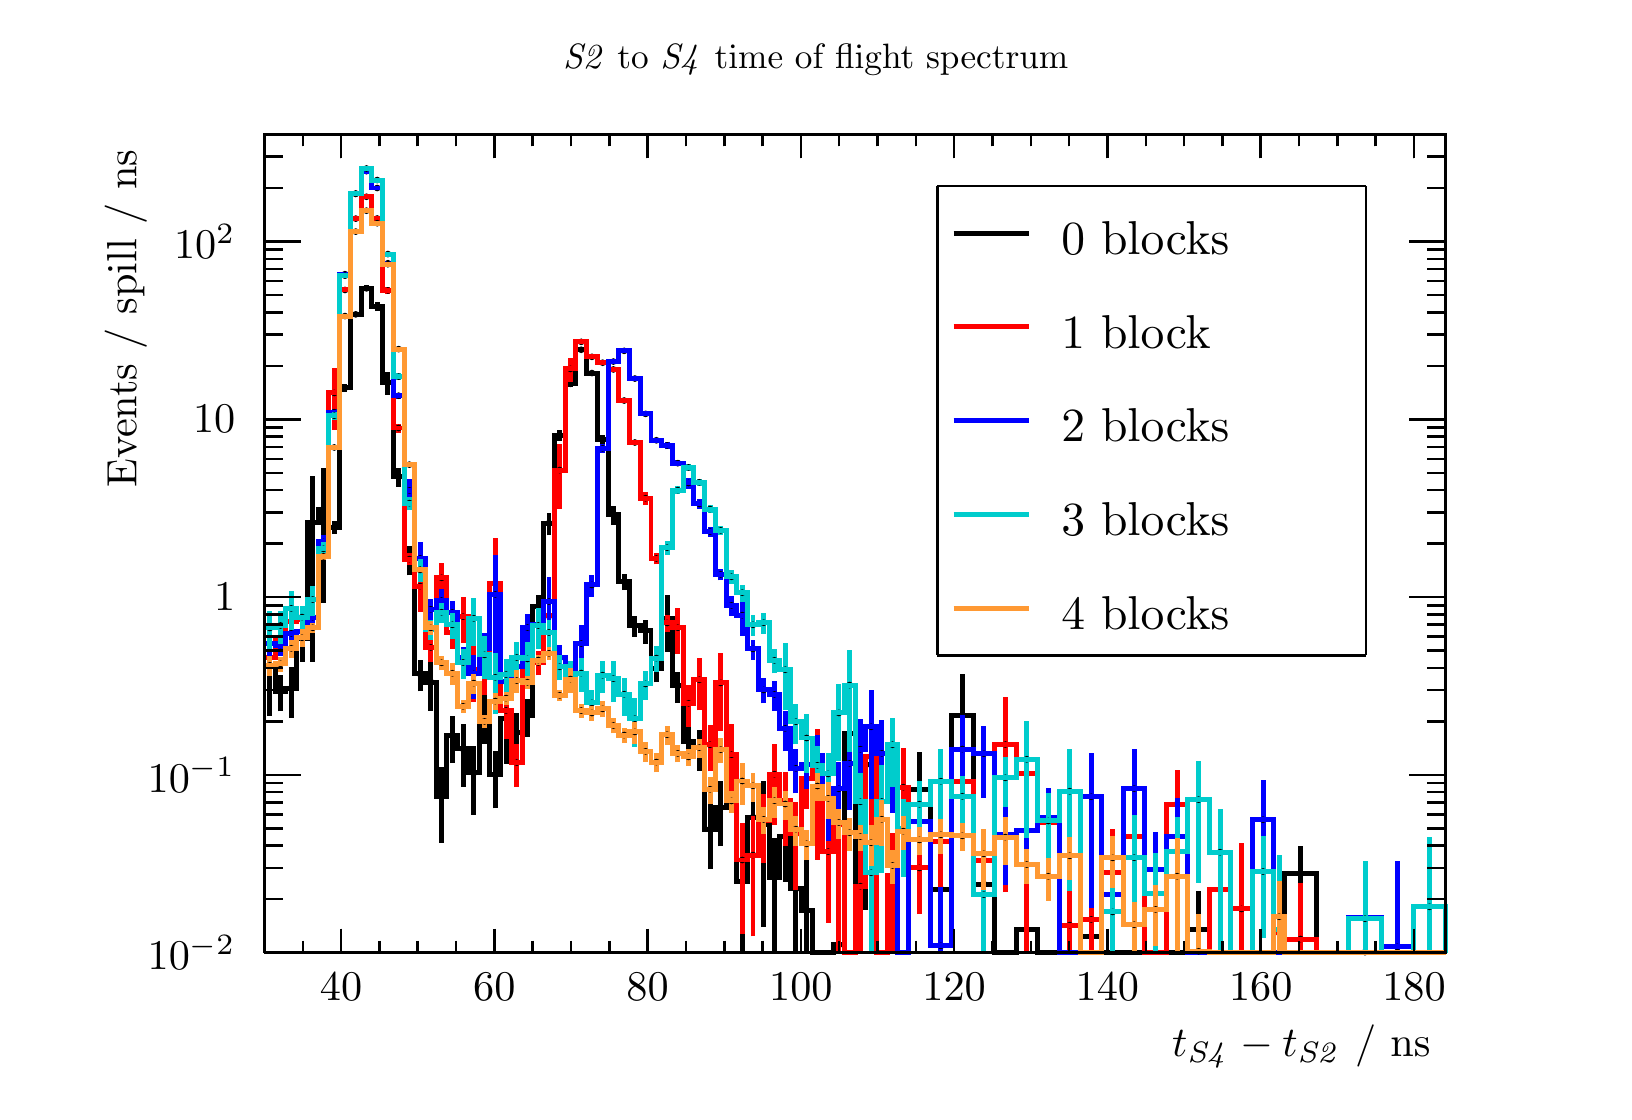
\begin{tikzpicture}
\pgfdeclareplotmark{cross} {
\pgfpathmoveto{\pgfpoint{-0.3\pgfplotmarksize}{\pgfplotmarksize}}
\pgfpathlineto{\pgfpoint{+0.3\pgfplotmarksize}{\pgfplotmarksize}}
\pgfpathlineto{\pgfpoint{+0.3\pgfplotmarksize}{0.3\pgfplotmarksize}}
\pgfpathlineto{\pgfpoint{+1\pgfplotmarksize}{0.3\pgfplotmarksize}}
\pgfpathlineto{\pgfpoint{+1\pgfplotmarksize}{-0.3\pgfplotmarksize}}
\pgfpathlineto{\pgfpoint{+0.3\pgfplotmarksize}{-0.3\pgfplotmarksize}}
\pgfpathlineto{\pgfpoint{+0.3\pgfplotmarksize}{-1.\pgfplotmarksize}}
\pgfpathlineto{\pgfpoint{-0.3\pgfplotmarksize}{-1.\pgfplotmarksize}}
\pgfpathlineto{\pgfpoint{-0.3\pgfplotmarksize}{-0.3\pgfplotmarksize}}
\pgfpathlineto{\pgfpoint{-1.\pgfplotmarksize}{-0.3\pgfplotmarksize}}
\pgfpathlineto{\pgfpoint{-1.\pgfplotmarksize}{0.3\pgfplotmarksize}}
\pgfpathlineto{\pgfpoint{-0.3\pgfplotmarksize}{0.3\pgfplotmarksize}}
\pgfpathclose
\pgfusepathqstroke
}
\pgfdeclareplotmark{cross*} {
\pgfpathmoveto{\pgfpoint{-0.3\pgfplotmarksize}{\pgfplotmarksize}}
\pgfpathlineto{\pgfpoint{+0.3\pgfplotmarksize}{\pgfplotmarksize}}
\pgfpathlineto{\pgfpoint{+0.3\pgfplotmarksize}{0.3\pgfplotmarksize}}
\pgfpathlineto{\pgfpoint{+1\pgfplotmarksize}{0.3\pgfplotmarksize}}
\pgfpathlineto{\pgfpoint{+1\pgfplotmarksize}{-0.3\pgfplotmarksize}}
\pgfpathlineto{\pgfpoint{+0.3\pgfplotmarksize}{-0.3\pgfplotmarksize}}
\pgfpathlineto{\pgfpoint{+0.3\pgfplotmarksize}{-1.\pgfplotmarksize}}
\pgfpathlineto{\pgfpoint{-0.3\pgfplotmarksize}{-1.\pgfplotmarksize}}
\pgfpathlineto{\pgfpoint{-0.3\pgfplotmarksize}{-0.3\pgfplotmarksize}}
\pgfpathlineto{\pgfpoint{-1.\pgfplotmarksize}{-0.3\pgfplotmarksize}}
\pgfpathlineto{\pgfpoint{-1.\pgfplotmarksize}{0.3\pgfplotmarksize}}
\pgfpathlineto{\pgfpoint{-0.3\pgfplotmarksize}{0.3\pgfplotmarksize}}
\pgfpathclose
\pgfusepathqfillstroke
}
\pgfdeclareplotmark{newstar} {
\pgfpathmoveto{\pgfqpoint{0pt}{\pgfplotmarksize}}
\pgfpathlineto{\pgfqpointpolar{44}{0.5\pgfplotmarksize}}
\pgfpathlineto{\pgfqpointpolar{18}{\pgfplotmarksize}}
\pgfpathlineto{\pgfqpointpolar{-20}{0.5\pgfplotmarksize}}
\pgfpathlineto{\pgfqpointpolar{-54}{\pgfplotmarksize}}
\pgfpathlineto{\pgfqpointpolar{-90}{0.5\pgfplotmarksize}}
\pgfpathlineto{\pgfqpointpolar{234}{\pgfplotmarksize}}
\pgfpathlineto{\pgfqpointpolar{198}{0.5\pgfplotmarksize}}
\pgfpathlineto{\pgfqpointpolar{162}{\pgfplotmarksize}}
\pgfpathlineto{\pgfqpointpolar{134}{0.5\pgfplotmarksize}}
\pgfpathclose
\pgfusepathqstroke
}
\pgfdeclareplotmark{newstar*} {
\pgfpathmoveto{\pgfqpoint{0pt}{\pgfplotmarksize}}
\pgfpathlineto{\pgfqpointpolar{44}{0.5\pgfplotmarksize}}
\pgfpathlineto{\pgfqpointpolar{18}{\pgfplotmarksize}}
\pgfpathlineto{\pgfqpointpolar{-20}{0.5\pgfplotmarksize}}
\pgfpathlineto{\pgfqpointpolar{-54}{\pgfplotmarksize}}
\pgfpathlineto{\pgfqpointpolar{-90}{0.5\pgfplotmarksize}}
\pgfpathlineto{\pgfqpointpolar{234}{\pgfplotmarksize}}
\pgfpathlineto{\pgfqpointpolar{198}{0.5\pgfplotmarksize}}
\pgfpathlineto{\pgfqpointpolar{162}{\pgfplotmarksize}}
\pgfpathlineto{\pgfqpointpolar{134}{0.5\pgfplotmarksize}}
\pgfpathclose
\pgfusepathqfillstroke
}
\definecolor{c}{rgb}{1,1,1};
\draw [color=c, fill=c] (0,0) rectangle (20,13.4957);
\draw [color=c, fill=c] (3,1.75444) rectangle (18,12.1461);
\definecolor{c}{rgb}{0,0,0};
\draw [c,line width=0.9] (3,1.75444) -- (3,12.1461) -- (18,12.1461) -- (18,1.75444) -- (3,1.75444);
\definecolor{c}{rgb}{1,1,1};
\draw [color=c, fill=c] (3,1.75444) rectangle (18,12.1461);
\definecolor{c}{rgb}{0,0,0};
\draw [c,line width=0.9] (3,1.75444) -- (3,12.1461) -- (18,12.1461) -- (18,1.75444) -- (3,1.75444);
\draw [c,line width=0.9] (3,1.75444) -- (3.13636,1.75444) -- (3.13636,1.75444) -- (3.27273,1.75444) -- (3.27273,1.75444) -- (3.40909,1.75444) -- (3.40909,1.75444) -- (3.54545,1.75444) -- (3.54545,1.75444) -- (3.68182,1.75444) -- (3.68182,1.75444) --
 (3.81818,1.75444) -- (3.81818,1.75444) -- (3.95455,1.75444) -- (3.95455,1.75444) -- (4.09091,1.75444) -- (4.09091,1.75444) -- (4.22727,1.75444) -- (4.22727,1.75444) -- (4.36364,1.75444) -- (4.36364,1.75444) -- (4.5,1.75444) -- (4.5,1.75444) --
 (4.63636,1.75444) -- (4.63636,1.75444) -- (4.77273,1.75444) -- (4.77273,1.75444) -- (4.90909,1.75444) -- (4.90909,1.75444) -- (5.04545,1.75444) -- (5.04545,1.75444) -- (5.18182,1.75444) -- (5.18182,1.75444) -- (5.31818,1.75444) -- (5.31818,1.75444)
 -- (5.45455,1.75444) -- (5.45455,1.75444) -- (5.59091,1.75444) -- (5.59091,1.75444) -- (5.72727,1.75444) -- (5.72727,1.75444) -- (5.86364,1.75444) -- (5.86364,1.75444) -- (6,1.75444) -- (6,1.75444) -- (6.13636,1.75444) -- (6.13636,1.75444) --
 (6.27273,1.75444) -- (6.27273,1.75444) -- (6.40909,1.75444) -- (6.40909,1.75444) -- (6.54545,1.75444) -- (6.54545,1.75444) -- (6.68182,1.75444) -- (6.68182,1.75444) -- (6.81818,1.75444) -- (6.81818,1.75444) -- (6.95455,1.75444) -- (6.95455,1.75444)
 -- (7.09091,1.75444) -- (7.09091,1.75444) -- (7.22727,1.75444) -- (7.22727,1.75444) -- (7.36364,1.75444) -- (7.36364,1.75444) -- (7.5,1.75444) -- (7.5,1.75444) -- (7.63636,1.75444) -- (7.63636,1.75444) -- (7.77273,1.75444) -- (7.77273,1.75444) --
 (7.90909,1.75444) -- (7.90909,1.75444) -- (8.04545,1.75444) -- (8.04545,1.75444) -- (8.18182,1.75444) -- (8.18182,1.75444) -- (8.31818,1.75444) -- (8.31818,1.75444) -- (8.45455,1.75444) -- (8.45455,1.75444) -- (8.59091,1.75444) -- (8.59091,1.75444)
 -- (8.72727,1.75444) -- (8.72727,1.75444) -- (8.86364,1.75444) -- (8.86364,1.75444) -- (9,1.75444) -- (9,1.75444) -- (9.13636,1.75444) -- (9.13636,1.75444) -- (9.27273,1.75444) -- (9.27273,1.75444) -- (9.40909,1.75444) -- (9.40909,1.75444) --
 (9.54545,1.75444) -- (9.54545,1.75444) -- (9.68182,1.75444) -- (9.68182,1.75444) -- (9.81818,1.75444) -- (9.81818,1.75444) -- (9.95455,1.75444) -- (9.95455,1.75444) -- (10.0909,1.75444) -- (10.0909,1.75444) -- (10.2273,1.75444) -- (10.2273,1.75444)
 -- (10.3636,1.75444) -- (10.3636,1.75444) -- (10.5,1.75444) -- (10.5,1.75444) -- (10.6364,1.75444) -- (10.6364,1.75444) -- (10.7727,1.75444) -- (10.7727,1.75444) -- (10.9091,1.75444) -- (10.9091,1.75444) -- (11.0455,1.75444) -- (11.0455,1.75444) --
 (11.1818,1.75444) -- (11.1818,1.75444) -- (11.4545,1.75444) -- (11.4545,1.75444) -- (11.7273,1.75444) -- (11.7273,1.75444) -- (12,1.75444) -- (12,1.75444) -- (12.2727,1.75444) -- (12.2727,1.75444) -- (12.5455,1.75444) -- (12.5455,1.75444) --
 (12.8182,1.75444) -- (12.8182,1.75444) -- (13.0909,1.75444) -- (13.0909,1.75444) -- (13.3636,1.75444) -- (13.3636,1.75444) -- (13.6364,1.75444) -- (13.6364,1.75444) -- (13.9091,1.75444) -- (13.9091,1.75444) -- (14.1818,1.75444) -- (14.1818,1.75444)
 -- (14.4545,1.75444) -- (14.4545,1.75444) -- (14.7273,1.75444) -- (14.7273,1.75444) -- (15,1.75444) -- (15,1.75444) -- (15.2727,1.75444) -- (15.2727,1.75444) -- (15.5455,1.75444) -- (15.5455,1.75444) -- (15.8182,1.75444) -- (15.8182,1.75444) --
 (15.9545,1.75444) -- (15.9545,1.75444) -- (16.3636,1.75444) -- (16.3636,1.75444) -- (16.7727,1.75444) -- (16.7727,1.75444) -- (17.1818,1.75444) -- (17.1818,1.75444) -- (17.5909,1.75444) -- (17.5909,1.75444) -- (18,1.75444);
\draw [c,line width=0.9] (3,1.75444) -- (18,1.75444);
\draw [c,line width=0.9] (3.97326,2.05809) -- (3.97326,1.75444);
\draw [c,line width=0.9] (4.45989,1.90627) -- (4.45989,1.75444);
\draw [c,line width=0.9] (4.94652,1.90627) -- (4.94652,1.75444);
\draw [c,line width=0.9] (5.43316,1.90627) -- (5.43316,1.75444);
\draw [c,line width=0.9] (5.91979,2.05809) -- (5.91979,1.75444);
\draw [c,line width=0.9] (6.40642,1.90627) -- (6.40642,1.75444);
\draw [c,line width=0.9] (6.89305,1.90627) -- (6.89305,1.75444);
\draw [c,line width=0.9] (7.37968,1.90627) -- (7.37968,1.75444);
\draw [c,line width=0.9] (7.86631,2.05809) -- (7.86631,1.75444);
\draw [c,line width=0.9] (8.35294,1.90627) -- (8.35294,1.75444);
\draw [c,line width=0.9] (8.83957,1.90627) -- (8.83957,1.75444);
\draw [c,line width=0.9] (9.3262,1.90627) -- (9.3262,1.75444);
\draw [c,line width=0.9] (9.81283,2.05809) -- (9.81283,1.75444);
\draw [c,line width=0.9] (10.2995,1.90627) -- (10.2995,1.75444);
\draw [c,line width=0.9] (10.7861,1.90627) -- (10.7861,1.75444);
\draw [c,line width=0.9] (11.2727,1.90627) -- (11.2727,1.75444);
\draw [c,line width=0.9] (11.7594,2.05809) -- (11.7594,1.75444);
\draw [c,line width=0.9] (12.246,1.90627) -- (12.246,1.75444);
\draw [c,line width=0.9] (12.7326,1.90627) -- (12.7326,1.75444);
\draw [c,line width=0.9] (13.2193,1.90627) -- (13.2193,1.75444);
\draw [c,line width=0.9] (13.7059,2.05809) -- (13.7059,1.75444);
\draw [c,line width=0.9] (14.1925,1.90627) -- (14.1925,1.75444);
\draw [c,line width=0.9] (14.6791,1.90627) -- (14.6791,1.75444);
\draw [c,line width=0.9] (15.1658,1.90627) -- (15.1658,1.75444);
\draw [c,line width=0.9] (15.6524,2.05809) -- (15.6524,1.75444);
\draw [c,line width=0.9] (16.139,1.90627) -- (16.139,1.75444);
\draw [c,line width=0.9] (16.6257,1.90627) -- (16.6257,1.75444);
\draw [c,line width=0.9] (17.1123,1.90627) -- (17.1123,1.75444);
\draw [c,line width=0.9] (17.5989,2.05809) -- (17.5989,1.75444);
\draw [c,line width=0.9] (3.97326,2.05809) -- (3.97326,1.75444);
\draw [c,line width=0.9] (3.48663,1.90627) -- (3.48663,1.75444);
\draw [c,line width=0.9] (3,1.90627) -- (3,1.75444);
\draw [c,line width=0.9] (17.5989,2.05809) -- (17.5989,1.75444);
\draw [anchor=base] (3.97326,1.14713) node[scale=1.52731, color=c, rotate=0]{40};
\draw [anchor=base] (5.91979,1.14713) node[scale=1.52731, color=c, rotate=0]{60};
\draw [anchor=base] (7.86631,1.14713) node[scale=1.52731, color=c, rotate=0]{80};
\draw [anchor=base] (9.81283,1.14713) node[scale=1.52731, color=c, rotate=0]{100};
\draw [anchor=base] (11.7594,1.14713) node[scale=1.52731, color=c, rotate=0]{120};
\draw [anchor=base] (13.7059,1.14713) node[scale=1.52731, color=c, rotate=0]{140};
\draw [anchor=base] (15.6524,1.14713) node[scale=1.52731, color=c, rotate=0]{160};
\draw [anchor=base] (17.5989,1.14713) node[scale=1.52731, color=c, rotate=0]{180};
\draw [anchor= east] (18,0.566819) node[scale=1.52731, color=c, rotate=0]{$ t_{\mathit{S4}} - t_{\mathit{S2}}$ / ns};
\draw [c,line width=0.9] (3,12.1461) -- (18,12.1461);
\draw [c,line width=0.9] (3.97326,11.8425) -- (3.97326,12.1461);
\draw [c,line width=0.9] (4.45989,11.9943) -- (4.45989,12.1461);
\draw [c,line width=0.9] (4.94652,11.9943) -- (4.94652,12.1461);
\draw [c,line width=0.9] (5.43316,11.9943) -- (5.43316,12.1461);
\draw [c,line width=0.9] (5.91979,11.8425) -- (5.91979,12.1461);
\draw [c,line width=0.9] (6.40642,11.9943) -- (6.40642,12.1461);
\draw [c,line width=0.9] (6.89305,11.9943) -- (6.89305,12.1461);
\draw [c,line width=0.9] (7.37968,11.9943) -- (7.37968,12.1461);
\draw [c,line width=0.9] (7.86631,11.8425) -- (7.86631,12.1461);
\draw [c,line width=0.9] (8.35294,11.9943) -- (8.35294,12.1461);
\draw [c,line width=0.9] (8.83957,11.9943) -- (8.83957,12.1461);
\draw [c,line width=0.9] (9.3262,11.9943) -- (9.3262,12.1461);
\draw [c,line width=0.9] (9.81283,11.8425) -- (9.81283,12.1461);
\draw [c,line width=0.9] (10.2995,11.9943) -- (10.2995,12.1461);
\draw [c,line width=0.9] (10.7861,11.9943) -- (10.7861,12.1461);
\draw [c,line width=0.9] (11.2727,11.9943) -- (11.2727,12.1461);
\draw [c,line width=0.9] (11.7594,11.8425) -- (11.7594,12.1461);
\draw [c,line width=0.9] (12.246,11.9943) -- (12.246,12.1461);
\draw [c,line width=0.9] (12.7326,11.9943) -- (12.7326,12.1461);
\draw [c,line width=0.9] (13.2193,11.9943) -- (13.2193,12.1461);
\draw [c,line width=0.9] (13.7059,11.8425) -- (13.7059,12.1461);
\draw [c,line width=0.9] (14.1925,11.9943) -- (14.1925,12.1461);
\draw [c,line width=0.9] (14.6791,11.9943) -- (14.6791,12.1461);
\draw [c,line width=0.9] (15.1658,11.9943) -- (15.1658,12.1461);
\draw [c,line width=0.9] (15.6524,11.8425) -- (15.6524,12.1461);
\draw [c,line width=0.9] (16.139,11.9943) -- (16.139,12.1461);
\draw [c,line width=0.9] (16.6257,11.9943) -- (16.6257,12.1461);
\draw [c,line width=0.9] (17.1123,11.9943) -- (17.1123,12.1461);
\draw [c,line width=0.9] (17.5989,11.8425) -- (17.5989,12.1461);
\draw [c,line width=0.9] (3.97326,11.8425) -- (3.97326,12.1461);
\draw [c,line width=0.9] (3.48663,11.9943) -- (3.48663,12.1461);
\draw [c,line width=0.9] (3,11.9943) -- (3,12.1461);
\draw [c,line width=0.9] (17.5989,11.8425) -- (17.5989,12.1461);
\draw [c,line width=0.9] (3,1.75444) -- (3,12.1461);
\draw [c,line width=0.9] (3.462,1.75444) -- (3,1.75444);
\draw [anchor= east] (2.82,1.75444) node[scale=1.52731, color=c, rotate=0]{$10^{-2}$};
\draw [c,line width=0.9] (3.231,2.43418) -- (3,2.43418);
\draw [c,line width=0.9] (3.231,2.83181) -- (3,2.83181);
\draw [c,line width=0.9] (3.231,3.11393) -- (3,3.11393);
\draw [c,line width=0.9] (3.231,3.33275) -- (3,3.33275);
\draw [c,line width=0.9] (3.231,3.51155) -- (3,3.51155);
\draw [c,line width=0.9] (3.231,3.66272) -- (3,3.66272);
\draw [c,line width=0.9] (3.231,3.79367) -- (3,3.79367);
\draw [c,line width=0.9] (3.231,3.90917) -- (3,3.90917);
\draw [c,line width=0.9] (3.462,4.0125) -- (3,4.0125);
\draw [anchor= east] (2.82,4.0125) node[scale=1.52731, color=c, rotate=0]{$10^{-1}$};
\draw [c,line width=0.9] (3.231,4.69224) -- (3,4.69224);
\draw [c,line width=0.9] (3.231,5.08986) -- (3,5.08986);
\draw [c,line width=0.9] (3.231,5.37198) -- (3,5.37198);
\draw [c,line width=0.9] (3.231,5.59081) -- (3,5.59081);
\draw [c,line width=0.9] (3.231,5.7696) -- (3,5.7696);
\draw [c,line width=0.9] (3.231,5.92077) -- (3,5.92077);
\draw [c,line width=0.9] (3.231,6.05172) -- (3,6.05172);
\draw [c,line width=0.9] (3.231,6.16722) -- (3,6.16722);
\draw [c,line width=0.9] (3.462,6.27055) -- (3,6.27055);
\draw [anchor= east] (2.82,6.27055) node[scale=1.52731, color=c, rotate=0]{1};
\draw [c,line width=0.9] (3.231,6.95029) -- (3,6.95029);
\draw [c,line width=0.9] (3.231,7.34791) -- (3,7.34791);
\draw [c,line width=0.9] (3.231,7.63003) -- (3,7.63003);
\draw [c,line width=0.9] (3.231,7.84886) -- (3,7.84886);
\draw [c,line width=0.9] (3.231,8.02765) -- (3,8.02765);
\draw [c,line width=0.9] (3.231,8.17882) -- (3,8.17882);
\draw [c,line width=0.9] (3.231,8.30977) -- (3,8.30977);
\draw [c,line width=0.9] (3.231,8.42527) -- (3,8.42527);
\draw [c,line width=0.9] (3.462,8.5286) -- (3,8.5286);
\draw [anchor= east] (2.82,8.5286) node[scale=1.52731, color=c, rotate=0]{10};
\draw [c,line width=0.9] (3.231,9.20834) -- (3,9.20834);
\draw [c,line width=0.9] (3.231,9.60596) -- (3,9.60596);
\draw [c,line width=0.9] (3.231,9.88808) -- (3,9.88808);
\draw [c,line width=0.9] (3.231,10.1069) -- (3,10.1069);
\draw [c,line width=0.9] (3.231,10.2857) -- (3,10.2857);
\draw [c,line width=0.9] (3.231,10.4369) -- (3,10.4369);
\draw [c,line width=0.9] (3.231,10.5678) -- (3,10.5678);
\draw [c,line width=0.9] (3.231,10.6833) -- (3,10.6833);
\draw [c,line width=0.9] (3.462,10.7866) -- (3,10.7866);
\draw [anchor= east] (2.82,10.7866) node[scale=1.52731, color=c, rotate=0]{$10^{2}$};
\draw [c,line width=0.9] (3.231,11.4664) -- (3,11.4664);
\draw [c,line width=0.9] (3.231,11.864) -- (3,11.864);
\draw [c,line width=0.9] (3.231,12.1461) -- (3,12.1461);
\draw [anchor= east] (1.24,12.1461) node[scale=1.52731, color=c, rotate=90]{ Events / spill / ns};
\draw [c,line width=0.9] (18,1.75444) -- (18,12.1461);
\draw [c,line width=0.9] (17.538,1.75444) -- (18,1.75444);
\draw [c,line width=0.9] (17.769,2.43418) -- (18,2.43418);
\draw [c,line width=0.9] (17.769,2.83181) -- (18,2.83181);
\draw [c,line width=0.9] (17.769,3.11393) -- (18,3.11393);
\draw [c,line width=0.9] (17.769,3.33275) -- (18,3.33275);
\draw [c,line width=0.9] (17.769,3.51155) -- (18,3.51155);
\draw [c,line width=0.9] (17.769,3.66272) -- (18,3.66272);
\draw [c,line width=0.9] (17.769,3.79367) -- (18,3.79367);
\draw [c,line width=0.9] (17.769,3.90917) -- (18,3.90917);
\draw [c,line width=0.9] (17.538,4.0125) -- (18,4.0125);
\draw [c,line width=0.9] (17.769,4.69224) -- (18,4.69224);
\draw [c,line width=0.9] (17.769,5.08986) -- (18,5.08986);
\draw [c,line width=0.9] (17.769,5.37198) -- (18,5.37198);
\draw [c,line width=0.9] (17.769,5.59081) -- (18,5.59081);
\draw [c,line width=0.9] (17.769,5.7696) -- (18,5.7696);
\draw [c,line width=0.9] (17.769,5.92077) -- (18,5.92077);
\draw [c,line width=0.9] (17.769,6.05172) -- (18,6.05172);
\draw [c,line width=0.9] (17.769,6.16722) -- (18,6.16722);
\draw [c,line width=0.9] (17.538,6.27055) -- (18,6.27055);
\draw [c,line width=0.9] (17.769,6.95029) -- (18,6.95029);
\draw [c,line width=0.9] (17.769,7.34791) -- (18,7.34791);
\draw [c,line width=0.9] (17.769,7.63003) -- (18,7.63003);
\draw [c,line width=0.9] (17.769,7.84886) -- (18,7.84886);
\draw [c,line width=0.9] (17.769,8.02765) -- (18,8.02765);
\draw [c,line width=0.9] (17.769,8.17882) -- (18,8.17882);
\draw [c,line width=0.9] (17.769,8.30977) -- (18,8.30977);
\draw [c,line width=0.9] (17.769,8.42527) -- (18,8.42527);
\draw [c,line width=0.9] (17.538,8.5286) -- (18,8.5286);
\draw [c,line width=0.9] (17.769,9.20834) -- (18,9.20834);
\draw [c,line width=0.9] (17.769,9.60596) -- (18,9.60596);
\draw [c,line width=0.9] (17.769,9.88808) -- (18,9.88808);
\draw [c,line width=0.9] (17.769,10.1069) -- (18,10.1069);
\draw [c,line width=0.9] (17.769,10.2857) -- (18,10.2857);
\draw [c,line width=0.9] (17.769,10.4369) -- (18,10.4369);
\draw [c,line width=0.9] (17.769,10.5678) -- (18,10.5678);
\draw [c,line width=0.9] (17.769,10.6833) -- (18,10.6833);
\draw [c,line width=0.9] (17.538,10.7866) -- (18,10.7866);
\draw [c,line width=0.9] (17.769,11.4664) -- (18,11.4664);
\draw [c,line width=0.9] (17.769,11.864) -- (18,11.864);
\draw [c,line width=0.9] (17.769,12.1461) -- (18,12.1461);
\draw [c,line width=1.8] (3.06818,4.76609) -- (3.06818,5.40071);
\draw [c,line width=1.8] (3.06818,5.40071) -- (3.06818,5.78282);
\foreach \P in {(3.06818,5.40071)}{\draw[mark options={color=c,fill=c},mark size=2.402402pt,mark=*,mark size=1pt] plot coordinates {\P};}
\draw [c,line width=1.8] (3.20455,4.81813) -- (3.20455,5.07538);
\draw [c,line width=1.8] (3.20455,5.07538) -- (3.20455,5.27899);
\foreach \P in {(3.20455,5.07538)}{\draw[mark options={color=c,fill=c},mark size=2.402402pt,mark=*,mark size=1pt] plot coordinates {\P};}
\draw [c,line width=1.8] (3.34091,4.73992) -- (3.34091,5.11562);
\draw [c,line width=1.8] (3.34091,5.11562) -- (3.34091,5.38659);
\foreach \P in {(3.34091,5.11562)}{\draw[mark options={color=c,fill=c},mark size=2.402402pt,mark=*,mark size=1pt] plot coordinates {\P};}
\draw [c,line width=1.8] (3.47727,5.45284) -- (3.47727,5.75063);
\draw [c,line width=1.8] (3.47727,5.75063) -- (3.47727,5.97875);
\foreach \P in {(3.47727,5.75063)}{\draw[mark options={color=c,fill=c},mark size=2.402402pt,mark=*,mark size=1pt] plot coordinates {\P};}
\draw [c,line width=1.8] (3.61364,5.449) -- (3.61364,7.21647);
\draw [c,line width=1.8] (3.61364,7.21647) -- (3.61364,7.81182);
\foreach \P in {(3.61364,7.21647)}{\draw[mark options={color=c,fill=c},mark size=2.402402pt,mark=*,mark size=1pt] plot coordinates {\P};}
\draw [c,line width=1.8] (3.75,6.19486) -- (3.75,7.38813);
\draw [c,line width=1.8] (3.75,7.38813) -- (3.75,7.9107);
\foreach \P in {(3.75,7.38813)}{\draw[mark options={color=c,fill=c},mark size=2.402402pt,mark=*,mark size=1pt] plot coordinates {\P};}
\draw [c,line width=1.8] (3.88636,7.07197) -- (3.88636,7.15962);
\draw [c,line width=1.8] (3.88636,7.15962) -- (3.88636,7.24007);
\foreach \P in {(3.88636,7.15962)}{\draw[mark options={color=c,fill=c},mark size=2.402402pt,mark=*,mark size=1pt] plot coordinates {\P};}
\draw [c,line width=1.8] (4.02273,8.88003) -- (4.02273,8.92947);
\draw [c,line width=1.8] (4.02273,8.92947) -- (4.02273,8.97653);
\foreach \P in {(4.02273,8.92947)}{\draw[mark options={color=c,fill=c},mark size=2.402402pt,mark=*,mark size=1pt] plot coordinates {\P};}
\draw [c,line width=1.8] (4.15909,9.82942) -- (4.15909,9.86175);
\draw [c,line width=1.8] (4.15909,9.86175) -- (4.15909,9.89304);
\foreach \P in {(4.15909,9.86175)}{\draw[mark options={color=c,fill=c},mark size=2.402402pt,mark=*,mark size=1pt] plot coordinates {\P};}
\draw [c,line width=1.8] (4.29545,10.154) -- (4.29545,10.1919);
\draw [c,line width=1.8] (4.29545,10.1919) -- (4.29545,10.2284);
\foreach \P in {(4.29545,10.1919)}{\draw[mark options={color=c,fill=c},mark size=2.402402pt,mark=*,mark size=1pt] plot coordinates {\P};}
\draw [c,line width=1.8] (4.43182,9.90216) -- (4.43182,9.96086);
\draw [c,line width=1.8] (4.43182,9.96086) -- (4.43182,10.0162);
\foreach \P in {(4.43182,9.96086)}{\draw[mark options={color=c,fill=c},mark size=2.402402pt,mark=*,mark size=1pt] plot coordinates {\P};}
\draw [c,line width=1.8] (4.56818,8.83982) -- (4.56818,8.9955);
\draw [c,line width=1.8] (4.56818,8.9955) -- (4.56818,9.12983);
\foreach \P in {(4.56818,8.9955)}{\draw[mark options={color=c,fill=c},mark size=2.402402pt,mark=*,mark size=1pt] plot coordinates {\P};}
\draw [c,line width=1.8] (4.70455,7.67461) -- (4.70455,7.80053);
\draw [c,line width=1.8] (4.70455,7.80053) -- (4.70455,7.9121);
\foreach \P in {(4.70455,7.80053)}{\draw[mark options={color=c,fill=c},mark size=2.402402pt,mark=*,mark size=1pt] plot coordinates {\P};}
\draw [c,line width=1.8] (4.84091,6.54749) -- (4.84091,6.75203);
\draw [c,line width=1.8] (4.84091,6.75203) -- (4.84091,6.92119);
\foreach \P in {(4.84091,6.75203)}{\draw[mark options={color=c,fill=c},mark size=2.402402pt,mark=*,mark size=1pt] plot coordinates {\P};}
\draw [c,line width=1.8] (4.97727,5.07239) -- (4.97727,5.29551);
\draw [c,line width=1.8] (4.97727,5.29551) -- (4.97727,5.47715);
\foreach \P in {(4.97727,5.29551)}{\draw[mark options={color=c,fill=c},mark size=2.402402pt,mark=*,mark size=1pt] plot coordinates {\P};}
\draw [c,line width=1.8] (5.11364,4.82747) -- (5.11364,5.19232);
\draw [c,line width=1.8] (5.11364,5.19232) -- (5.11364,5.45764);
\foreach \P in {(5.11364,5.19232)}{\draw[mark options={color=c,fill=c},mark size=2.402402pt,mark=*,mark size=1pt] plot coordinates {\P};}
\draw [c,line width=1.8] (5.25,3.1514) -- (5.25,3.74222);
\draw [c,line width=1.8] (5.25,3.74222) -- (5.25,4.10832);
\foreach \P in {(5.25,3.74222)}{\draw[mark options={color=c,fill=c},mark size=2.402402pt,mark=*,mark size=1pt] plot coordinates {\P};}
\draw [c,line width=1.8] (5.38636,4.16357) -- (5.38636,4.5075);
\draw [c,line width=1.8] (5.38636,4.5075) -- (5.38636,4.76162);
\foreach \P in {(5.38636,4.5075)}{\draw[mark options={color=c,fill=c},mark size=2.402402pt,mark=*,mark size=1pt] plot coordinates {\P};}
\draw [c,line width=1.8] (5.52273,3.86174) -- (5.52273,4.34356);
\draw [c,line width=1.8] (5.52273,4.34356) -- (5.52273,4.66522);
\foreach \P in {(5.52273,4.34356)}{\draw[mark options={color=c,fill=c},mark size=2.402402pt,mark=*,mark size=1pt] plot coordinates {\P};}
\draw [c,line width=1.8] (5.65909,3.50879) -- (5.65909,4.03798);
\draw [c,line width=1.8] (5.65909,4.03798) -- (5.65909,4.3798);
\foreach \P in {(5.65909,4.03798)}{\draw[mark options={color=c,fill=c},mark size=2.402402pt,mark=*,mark size=1pt] plot coordinates {\P};}
\draw [c,line width=1.8] (5.79545,4.41003) -- (5.79545,4.93593);
\draw [c,line width=1.8] (5.79545,4.93593) -- (5.79545,5.2764);
\foreach \P in {(5.79545,4.93593)}{\draw[mark options={color=c,fill=c},mark size=2.402402pt,mark=*,mark size=1pt] plot coordinates {\P};}
\draw [c,line width=1.8] (5.93182,3.5884) -- (5.93182,4.01749);
\draw [c,line width=1.8] (5.93182,4.01749) -- (5.93182,4.31497);
\foreach \P in {(5.93182,4.01749)}{\draw[mark options={color=c,fill=c},mark size=2.402402pt,mark=*,mark size=1pt] plot coordinates {\P};}
\draw [c,line width=1.8] (6.06818,4.15217) -- (6.06818,4.72752);
\draw [c,line width=1.8] (6.06818,4.72752) -- (6.06818,5.08772);
\foreach \P in {(6.06818,4.72752)}{\draw[mark options={color=c,fill=c},mark size=2.402402pt,mark=*,mark size=1pt] plot coordinates {\P};}
\draw [c,line width=1.8] (6.20455,4.21678) -- (6.20455,4.54867);
\draw [c,line width=1.8] (6.20455,4.54867) -- (6.20455,4.79619);
\foreach \P in {(6.20455,4.54867)}{\draw[mark options={color=c,fill=c},mark size=2.402402pt,mark=*,mark size=1pt] plot coordinates {\P};}
\draw [c,line width=1.8] (6.34091,4.49376) -- (6.34091,4.76233);
\draw [c,line width=1.8] (6.34091,4.76233) -- (6.34091,4.97294);
\foreach \P in {(6.34091,4.76233)}{\draw[mark options={color=c,fill=c},mark size=2.402402pt,mark=*,mark size=1pt] plot coordinates {\P};}
\draw [c,line width=1.8] (6.47727,5.96589) -- (6.47727,6.14792);
\draw [c,line width=1.8] (6.47727,6.14792) -- (6.47727,6.30138);
\foreach \P in {(6.47727,6.14792)}{\draw[mark options={color=c,fill=c},mark size=2.402402pt,mark=*,mark size=1pt] plot coordinates {\P};}
\draw [c,line width=1.8] (6.61364,7.05608) -- (6.61364,7.21099);
\draw [c,line width=1.8] (6.61364,7.21099) -- (6.61364,7.34473);
\foreach \P in {(6.61364,7.21099)}{\draw[mark options={color=c,fill=c},mark size=2.402402pt,mark=*,mark size=1pt] plot coordinates {\P};}
\draw [c,line width=1.8] (6.75,8.25554) -- (6.75,8.32543);
\draw [c,line width=1.8] (6.75,8.32543) -- (6.75,8.39067);
\foreach \P in {(6.75,8.32543)}{\draw[mark options={color=c,fill=c},mark size=2.402402pt,mark=*,mark size=1pt] plot coordinates {\P};}
\draw [c,line width=1.8] (6.88636,8.93919) -- (6.88636,8.9794);
\draw [c,line width=1.8] (6.88636,8.9794) -- (6.88636,9.01803);
\foreach \P in {(6.88636,8.9794)}{\draw[mark options={color=c,fill=c},mark size=2.402402pt,mark=*,mark size=1pt] plot coordinates {\P};}
\draw [c,line width=1.8] (7.02273,9.38097) -- (7.02273,9.4121);
\draw [c,line width=1.8] (7.02273,9.4121) -- (7.02273,9.44229);
\foreach \P in {(7.02273,9.4121)}{\draw[mark options={color=c,fill=c},mark size=2.402402pt,mark=*,mark size=1pt] plot coordinates {\P};}
\draw [c,line width=1.8] (7.15909,9.08494) -- (7.15909,9.11642);
\draw [c,line width=1.8] (7.15909,9.11642) -- (7.15909,9.14691);
\foreach \P in {(7.15909,9.11642)}{\draw[mark options={color=c,fill=c},mark size=2.402402pt,mark=*,mark size=1pt] plot coordinates {\P};}
\draw [c,line width=1.8] (7.29545,8.21148) -- (7.29545,8.26959);
\draw [c,line width=1.8] (7.29545,8.26959) -- (7.29545,8.32444);
\foreach \P in {(7.29545,8.26959)}{\draw[mark options={color=c,fill=c},mark size=2.402402pt,mark=*,mark size=1pt] plot coordinates {\P};}
\draw [c,line width=1.8] (7.43182,7.18629) -- (7.43182,7.31557);
\draw [c,line width=1.8] (7.43182,7.31557) -- (7.43182,7.42978);
\foreach \P in {(7.43182,7.31557)}{\draw[mark options={color=c,fill=c},mark size=2.402402pt,mark=*,mark size=1pt] plot coordinates {\P};}
\draw [c,line width=1.8] (7.56818,6.36075) -- (7.56818,6.46737);
\draw [c,line width=1.8] (7.56818,6.46737) -- (7.56818,6.56353);
\foreach \P in {(7.56818,6.46737)}{\draw[mark options={color=c,fill=c},mark size=2.402402pt,mark=*,mark size=1pt] plot coordinates {\P};}
\draw [c,line width=1.8] (7.70455,5.76677) -- (7.70455,5.90731);
\draw [c,line width=1.8] (7.70455,5.90731) -- (7.70455,6.03021);
\foreach \P in {(7.70455,5.90731)}{\draw[mark options={color=c,fill=c},mark size=2.402402pt,mark=*,mark size=1pt] plot coordinates {\P};}
\draw [c,line width=1.8] (7.84091,5.68052) -- (7.84091,5.84053);
\draw [c,line width=1.8] (7.84091,5.84053) -- (7.84091,5.97806);
\foreach \P in {(7.84091,5.84053)}{\draw[mark options={color=c,fill=c},mark size=2.402402pt,mark=*,mark size=1pt] plot coordinates {\P};}
\draw [c,line width=1.8] (7.97727,5.18881) -- (7.97727,5.36403);
\draw [c,line width=1.8] (7.97727,5.36403) -- (7.97727,5.51263);
\foreach \P in {(7.97727,5.36403)}{\draw[mark options={color=c,fill=c},mark size=2.402402pt,mark=*,mark size=1pt] plot coordinates {\P};}
\draw [c,line width=1.8] (8.11364,5.57089) -- (8.11364,5.99723);
\draw [c,line width=1.8] (8.11364,5.99723) -- (8.11364,6.2934);
\foreach \P in {(8.11364,5.99723)}{\draw[mark options={color=c,fill=c},mark size=2.402402pt,mark=*,mark size=1pt] plot coordinates {\P};}
\draw [c,line width=1.8] (8.25,4.92407) -- (8.25,5.14459);
\draw [c,line width=1.8] (8.25,5.14459) -- (8.25,5.32452);
\foreach \P in {(8.25,5.14459)}{\draw[mark options={color=c,fill=c},mark size=2.402402pt,mark=*,mark size=1pt] plot coordinates {\P};}
\draw [c,line width=1.8] (8.38636,4.16029) -- (8.38636,4.44129);
\draw [c,line width=1.8] (8.38636,4.44129) -- (8.38636,4.65946);
\foreach \P in {(8.38636,4.44129)}{\draw[mark options={color=c,fill=c},mark size=2.402402pt,mark=*,mark size=1pt] plot coordinates {\P};}
\draw [c,line width=1.8] (8.52273,4.06661) -- (8.52273,4.36117);
\draw [c,line width=1.8] (8.52273,4.36117) -- (8.52273,4.58738);
\foreach \P in {(8.52273,4.36117)}{\draw[mark options={color=c,fill=c},mark size=2.402402pt,mark=*,mark size=1pt] plot coordinates {\P};}
\draw [c,line width=1.8] (8.65909,2.81519) -- (8.65909,3.32407);
\draw [c,line width=1.8] (8.65909,3.32407) -- (8.65909,3.65741);
\foreach \P in {(8.65909,3.32407)}{\draw[mark options={color=c,fill=c},mark size=2.402402pt,mark=*,mark size=1pt] plot coordinates {\P};}
\draw [c,line width=1.8] (8.79545,3.10577) -- (8.79545,3.60233);
\draw [c,line width=1.8] (8.79545,3.60233) -- (8.79545,3.93041);
\foreach \P in {(8.79545,3.60233)}{\draw[mark options={color=c,fill=c},mark size=2.402402pt,mark=*,mark size=1pt] plot coordinates {\P};}
\draw [c,line width=1.8] (8.93182,3.55905) -- (8.93182,3.96429);
\draw [c,line width=1.8] (8.93182,3.96429) -- (8.93182,4.2502);
\foreach \P in {(8.93182,3.96429)}{\draw[mark options={color=c,fill=c},mark size=2.402402pt,mark=*,mark size=1pt] plot coordinates {\P};}
\draw [c,line width=1.8] (9.06818,1.75444) -- (9.06818,2.66362);
\draw [c,line width=1.8] (9.06818,2.66362) -- (9.06818,3.13843);
\foreach \P in {(9.06818,2.66362)}{\draw[mark options={color=c,fill=c},mark size=2.402402pt,mark=*,mark size=1pt] plot coordinates {\P};}
\draw [c,line width=1.8] (9.20455,2.5118) -- (9.20455,3.47595);
\draw [c,line width=1.8] (9.20455,3.47595) -- (9.20455,3.95259);
\foreach \P in {(9.20455,3.47595)}{\draw[mark options={color=c,fill=c},mark size=2.402402pt,mark=*,mark size=1pt] plot coordinates {\P};}
\draw [c,line width=1.8] (9.34091,2.07979) -- (9.34091,3.38794);
\draw [c,line width=1.8] (9.34091,3.38794) -- (9.34091,3.92918);
\foreach \P in {(9.34091,3.38794)}{\draw[mark options={color=c,fill=c},mark size=2.402402pt,mark=*,mark size=1pt] plot coordinates {\P};}
\draw [c,line width=1.8] (9.47727,1.75444) -- (9.47727,2.70847);
\draw [c,line width=1.8] (9.47727,2.70847) -- (9.47727,3.20782);
\foreach \P in {(9.47727,2.70847)}{\draw[mark options={color=c,fill=c},mark size=2.402402pt,mark=*,mark size=1pt] plot coordinates {\P};}
\draw [c,line width=1.8] (9.61364,2.65473) -- (9.61364,3.22579);
\draw [c,line width=1.8] (9.61364,3.22579) -- (9.61364,3.58434);
\foreach \P in {(9.61364,3.22579)}{\draw[mark options={color=c,fill=c},mark size=2.402402pt,mark=*,mark size=1pt] plot coordinates {\P};}
\draw [c,line width=1.8] (9.75,1.75444) -- (9.75,2.5657);
\draw [c,line width=1.8] (9.75,2.5657) -- (9.75,3.13049);
\foreach \P in {(9.75,2.5657)}{\draw[mark options={color=c,fill=c},mark size=2.402402pt,mark=*,mark size=1pt] plot coordinates {\P};}
\draw [c,line width=1.8] (9.88636,1.75444) -- (9.88636,2.29435);
\draw [c,line width=1.8] (9.88636,2.29435) -- (9.88636,2.93345);
\foreach \P in {(9.88636,2.29435)}{\draw[mark options={color=c,fill=c},mark size=2.402402pt,mark=*,mark size=1pt] plot coordinates {\P};}
\draw [c,line width=1.8] (10.2955,1.75444) -- (10.2955,1.85363);
\draw [c,line width=1.8] (10.2955,1.85363) -- (10.2955,2.70931);
\foreach \P in {(10.2955,1.85363)}{\draw[mark options={color=c,fill=c},mark size=2.402402pt,mark=*,mark size=1pt] plot coordinates {\P};}
\draw [c,line width=1.8] (10.4318,3.89762) -- (10.4318,4.53775);
\draw [c,line width=1.8] (10.4318,4.53775) -- (10.4318,4.9218);
\foreach \P in {(10.4318,4.53775)}{\draw[mark options={color=c,fill=c},mark size=2.402402pt,mark=*,mark size=1pt] plot coordinates {\P};}
\draw [c,line width=1.8] (10.5682,1.75444) -- (10.5682,2.32852);
\draw [c,line width=1.8] (10.5682,2.32852) -- (10.5682,2.95257);
\foreach \P in {(10.5682,2.32852)}{\draw[mark options={color=c,fill=c},mark size=2.402402pt,mark=*,mark size=1pt] plot coordinates {\P};}
\draw [c,line width=1.8] (10.7045,2.48834) -- (10.7045,4.13941);
\draw [c,line width=1.8] (10.7045,4.13941) -- (10.7045,4.72359);
\foreach \P in {(10.7045,4.13941)}{\draw[mark options={color=c,fill=c},mark size=2.402402pt,mark=*,mark size=1pt] plot coordinates {\P};}
\draw [c,line width=1.8] (10.9773,1.75444) -- (10.9773,1.87341);
\draw [c,line width=1.8] (10.9773,1.87341) -- (10.9773,2.5613);
\foreach \P in {(10.9773,1.87341)}{\draw[mark options={color=c,fill=c},mark size=2.402402pt,mark=*,mark size=1pt] plot coordinates {\P};}
\draw [c,line width=1.8] (11.3182,2.84284) -- (11.3182,3.82365);
\draw [c,line width=1.8] (11.3182,3.82365) -- (11.3182,4.30409);
\foreach \P in {(11.3182,3.82365)}{\draw[mark options={color=c,fill=c},mark size=2.402402pt,mark=*,mark size=1pt] plot coordinates {\P};}
\draw [c,line width=1.8] (11.5909,1.75444) -- (11.5909,2.56333);
\draw [c,line width=1.8] (11.5909,2.56333) -- (11.5909,3.10203);
\foreach \P in {(11.5909,2.56333)}{\draw[mark options={color=c,fill=c},mark size=2.402402pt,mark=*,mark size=1pt] plot coordinates {\P};}
\draw [c,line width=1.8] (11.8636,3.55441) -- (11.8636,4.76849);
\draw [c,line width=1.8] (11.8636,4.76849) -- (11.8636,5.29463);
\foreach \P in {(11.8636,4.76849)}{\draw[mark options={color=c,fill=c},mark size=2.402402pt,mark=*,mark size=1pt] plot coordinates {\P};}
\draw [c,line width=1.8] (12.1364,2.01506) -- (12.1364,2.62662);
\draw [c,line width=1.8] (12.1364,2.62662) -- (12.1364,3.00042);
\foreach \P in {(12.1364,2.62662)}{\draw[mark options={color=c,fill=c},mark size=2.402402pt,mark=*,mark size=1pt] plot coordinates {\P};}
\draw [c,line width=1.8] (12.6818,1.75444) -- (12.6818,2.04415);
\draw [c,line width=1.8] (12.6818,2.04415) -- (12.6818,2.63026);
\foreach \P in {(12.6818,2.04415)}{\draw[mark options={color=c,fill=c},mark size=2.402402pt,mark=*,mark size=1pt] plot coordinates {\P};}
\draw [c,line width=1.8] (13.5,1.75444) -- (13.5,1.96165);
\draw [c,line width=1.8] (13.5,1.96165) -- (13.5,2.49672);
\foreach \P in {(13.5,1.96165)}{\draw[mark options={color=c,fill=c},mark size=2.402402pt,mark=*,mark size=1pt] plot coordinates {\P};}
\draw [c,line width=1.8] (14.8636,1.75444) -- (14.8636,2.05116);
\draw [c,line width=1.8] (14.8636,2.05116) -- (14.8636,2.5321);
\foreach \P in {(14.8636,2.05116)}{\draw[mark options={color=c,fill=c},mark size=2.402402pt,mark=*,mark size=1pt] plot coordinates {\P};}
\draw [c,line width=1.8] (16.1591,2.1963) -- (16.1591,2.75613);
\draw [c,line width=1.8] (16.1591,2.75613) -- (16.1591,3.11029);
\foreach \P in {(16.1591,2.75613)}{\draw[mark options={color=c,fill=c},mark size=2.402402pt,mark=*,mark size=1pt] plot coordinates {\P};}
\draw [c,line width=1.8] (16.9773,1.75444) -- (16.9773,1.76166);
\draw [c,line width=1.8] (16.9773,1.76166) -- (16.9773,2.23418);
\foreach \P in {(16.9773,1.76166)}{\draw[mark options={color=c,fill=c},mark size=2.402402pt,mark=*,mark size=1pt] plot coordinates {\P};}
\draw [c,line width=1.8] (3,5.40071) -- (3.13636,5.40071) -- (3.13636,5.07538) -- (3.27273,5.07538) -- (3.27273,5.11562) -- (3.40909,5.11562) -- (3.40909,5.75063) -- (3.54545,5.75063) -- (3.54545,7.21647) -- (3.68182,7.21647) -- (3.68182,7.38813) --
 (3.81818,7.38813) -- (3.81818,7.15962) -- (3.95455,7.15962) -- (3.95455,8.92947) -- (4.09091,8.92947) -- (4.09091,9.86175) -- (4.22727,9.86175) -- (4.22727,10.1919) -- (4.36364,10.1919) -- (4.36364,9.96086) -- (4.5,9.96086) -- (4.5,8.9955) --
 (4.63636,8.9955) -- (4.63636,7.80053) -- (4.77273,7.80053) -- (4.77273,6.75203) -- (4.90909,6.75203) -- (4.90909,5.29551) -- (5.04545,5.29551) -- (5.04545,5.19232) -- (5.18182,5.19232) -- (5.18182,3.74222) -- (5.31818,3.74222) -- (5.31818,4.5075) --
 (5.45455,4.5075) -- (5.45455,4.34356) -- (5.59091,4.34356) -- (5.59091,4.03798) -- (5.72727,4.03798) -- (5.72727,4.93593) -- (5.86364,4.93593) -- (5.86364,4.01749) -- (6,4.01749) -- (6,4.72752) -- (6.13636,4.72752) -- (6.13636,4.54867) --
 (6.27273,4.54867) -- (6.27273,4.76233) -- (6.40909,4.76233) -- (6.40909,6.14792) -- (6.54545,6.14792) -- (6.54545,7.21099) -- (6.68182,7.21099) -- (6.68182,8.32543) -- (6.81818,8.32543) -- (6.81818,8.9794) -- (6.95455,8.9794) -- (6.95455,9.4121) --
 (7.09091,9.4121) -- (7.09091,9.11642) -- (7.22727,9.11642) -- (7.22727,8.26959) -- (7.36364,8.26959) -- (7.36364,7.31557) -- (7.5,7.31557) -- (7.5,6.46737) -- (7.63636,6.46737) -- (7.63636,5.90731) -- (7.77273,5.90731) -- (7.77273,5.84053) --
 (7.90909,5.84053) -- (7.90909,5.36403) -- (8.04545,5.36403) -- (8.04545,5.99723) -- (8.18182,5.99723) -- (8.18182,5.14459) -- (8.31818,5.14459) -- (8.31818,4.44129) -- (8.45455,4.44129) -- (8.45455,4.36117) -- (8.59091,4.36117) -- (8.59091,3.32407)
 -- (8.72727,3.32407) -- (8.72727,3.60233) -- (8.86364,3.60233) -- (8.86364,3.96429) -- (9,3.96429) -- (9,2.66362) -- (9.13636,2.66362) -- (9.13636,3.47595) -- (9.27273,3.47595) -- (9.27273,3.38794) -- (9.40909,3.38794) -- (9.40909,2.70847) --
 (9.54545,2.70847) -- (9.54545,3.22579) -- (9.68182,3.22579) -- (9.68182,2.5657) -- (9.81818,2.5657) -- (9.81818,2.29435) -- (9.95455,2.29435) -- (9.95455,1.75444) -- (10.0909,1.75444) -- (10.0909,1.75444) -- (10.2273,1.75444) -- (10.2273,1.85363) --
 (10.3636,1.85363) -- (10.3636,4.53775) -- (10.5,4.53775) -- (10.5,2.32852) -- (10.6364,2.32852) -- (10.6364,4.13941) -- (10.7727,4.13941) -- (10.7727,1.75444) -- (10.9091,1.75444) -- (10.9091,1.87341) -- (11.0455,1.87341) -- (11.0455,1.75444) --
 (11.1818,1.75444) -- (11.1818,3.82365) -- (11.4545,3.82365) -- (11.4545,2.56333) -- (11.7273,2.56333) -- (11.7273,4.76849) -- (12,4.76849) -- (12,2.62662) -- (12.2727,2.62662) -- (12.2727,1.75444) -- (12.5455,1.75444) -- (12.5455,2.04415) --
 (12.8182,2.04415) -- (12.8182,1.75444) -- (13.0909,1.75444) -- (13.0909,1.75444) -- (13.3636,1.75444) -- (13.3636,1.96165) -- (13.6364,1.96165) -- (13.6364,1.75444) -- (13.9091,1.75444) -- (13.9091,1.75444) -- (14.1818,1.75444) -- (14.1818,1.75444)
 -- (14.4545,1.75444) -- (14.4545,1.75444) -- (14.7273,1.75444) -- (14.7273,2.05116) -- (15,2.05116) -- (15,1.75444) -- (15.2727,1.75444) -- (15.2727,1.75444) -- (15.5455,1.75444) -- (15.5455,1.75444) -- (15.8182,1.75444) -- (15.8182,1.75444) --
 (15.9545,1.75444) -- (15.9545,2.75613) -- (16.3636,2.75613) -- (16.3636,1.75444) -- (16.7727,1.75444) -- (16.7727,1.76166) -- (17.1818,1.76166) -- (17.1818,1.75444) -- (17.5909,1.75444) -- (17.5909,1.75444) -- (18,1.75444) -- (18,1.75444) --
 (18,1.75444);
\definecolor{c}{rgb}{1,0,0};
\draw [c,line width=1.8] (3.06818,5.31503) -- (3.06818,5.50359);
\draw [c,line width=1.8] (3.06818,5.50359) -- (3.06818,5.66167);
\definecolor{c}{rgb}{0,0,0};
\foreach \P in {(3.06818,5.50359)}{\draw[mark options={color=c,fill=c},mark size=2.402402pt,mark=*,mark size=1pt] plot coordinates {\P};}
\definecolor{c}{rgb}{1,0,0};
\draw [c,line width=1.8] (3.20455,5.51789) -- (3.20455,5.73081);
\draw [c,line width=1.8] (3.20455,5.73081) -- (3.20455,5.90565);
\definecolor{c}{rgb}{0,0,0};
\foreach \P in {(3.20455,5.73081)}{\draw[mark options={color=c,fill=c},mark size=2.402402pt,mark=*,mark size=1pt] plot coordinates {\P};}
\definecolor{c}{rgb}{1,0,0};
\draw [c,line width=1.8] (3.34091,5.71062) -- (3.34091,5.9602);
\draw [c,line width=1.8] (3.34091,5.9602) -- (3.34091,6.15898);
\definecolor{c}{rgb}{0,0,0};
\foreach \P in {(3.34091,5.9602)}{\draw[mark options={color=c,fill=c},mark size=2.402402pt,mark=*,mark size=1pt] plot coordinates {\P};}
\definecolor{c}{rgb}{1,0,0};
\draw [c,line width=1.8] (3.47727,5.80459) -- (3.47727,5.99176);
\draw [c,line width=1.8] (3.47727,5.99176) -- (3.47727,6.14886);
\definecolor{c}{rgb}{0,0,0};
\foreach \P in {(3.47727,5.99176)}{\draw[mark options={color=c,fill=c},mark size=2.402402pt,mark=*,mark size=1pt] plot coordinates {\P};}
\definecolor{c}{rgb}{1,0,0};
\draw [c,line width=1.8] (3.61364,6.04894) -- (3.61364,6.24003);
\draw [c,line width=1.8] (3.61364,6.24003) -- (3.61364,6.39989);
\definecolor{c}{rgb}{0,0,0};
\foreach \P in {(3.61364,6.24003)}{\draw[mark options={color=c,fill=c},mark size=2.402402pt,mark=*,mark size=1pt] plot coordinates {\P};}
\definecolor{c}{rgb}{1,0,0};
\draw [c,line width=1.8] (3.75,6.78762) -- (3.75,6.8854);
\draw [c,line width=1.8] (3.75,6.8854) -- (3.75,6.97431);
\definecolor{c}{rgb}{0,0,0};
\foreach \P in {(3.75,6.8854)}{\draw[mark options={color=c,fill=c},mark size=2.402402pt,mark=*,mark size=1pt] plot coordinates {\P};}
\definecolor{c}{rgb}{1,0,0};
\draw [c,line width=1.8] (3.88636,8.39459) -- (3.88636,8.86392);
\draw [c,line width=1.8] (3.88636,8.86392) -- (3.88636,9.18001);
\definecolor{c}{rgb}{0,0,0};
\foreach \P in {(3.88636,8.86392)}{\draw[mark options={color=c,fill=c},mark size=2.402402pt,mark=*,mark size=1pt] plot coordinates {\P};}
\definecolor{c}{rgb}{1,0,0};
\draw [c,line width=1.8] (4.02273,10.1503) -- (4.02273,10.1714);
\draw [c,line width=1.8] (4.02273,10.1714) -- (4.02273,10.192);
\definecolor{c}{rgb}{0,0,0};
\foreach \P in {(4.02273,10.1714)}{\draw[mark options={color=c,fill=c},mark size=2.402402pt,mark=*,mark size=1pt] plot coordinates {\P};}
\definecolor{c}{rgb}{1,0,0};
\draw [c,line width=1.8] (4.15909,11.0601) -- (4.15909,11.0775);
\draw [c,line width=1.8] (4.15909,11.0775) -- (4.15909,11.0945);
\definecolor{c}{rgb}{0,0,0};
\foreach \P in {(4.15909,11.0775)}{\draw[mark options={color=c,fill=c},mark size=2.402402pt,mark=*,mark size=1pt] plot coordinates {\P};}
\definecolor{c}{rgb}{1,0,0};
\draw [c,line width=1.8] (4.29545,11.3343) -- (4.29545,11.3553);
\draw [c,line width=1.8] (4.29545,11.3553) -- (4.29545,11.3759);
\definecolor{c}{rgb}{0,0,0};
\foreach \P in {(4.29545,11.3553)}{\draw[mark options={color=c,fill=c},mark size=2.402402pt,mark=*,mark size=1pt] plot coordinates {\P};}
\definecolor{c}{rgb}{1,0,0};
\draw [c,line width=1.8] (4.43182,11.0544) -- (4.43182,11.079);
\draw [c,line width=1.8] (4.43182,11.079) -- (4.43182,11.103);
\definecolor{c}{rgb}{0,0,0};
\foreach \P in {(4.43182,11.079)}{\draw[mark options={color=c,fill=c},mark size=2.402402pt,mark=*,mark size=1pt] plot coordinates {\P};}
\definecolor{c}{rgb}{1,0,0};
\draw [c,line width=1.8] (4.56818,10.1229) -- (4.56818,10.1655);
\draw [c,line width=1.8] (4.56818,10.1655) -- (4.56818,10.2063);
\definecolor{c}{rgb}{0,0,0};
\foreach \P in {(4.56818,10.1655)}{\draw[mark options={color=c,fill=c},mark size=2.402402pt,mark=*,mark size=1pt] plot coordinates {\P};}
\definecolor{c}{rgb}{1,0,0};
\draw [c,line width=1.8] (4.70455,8.36012) -- (4.70455,8.4186);
\draw [c,line width=1.8] (4.70455,8.4186) -- (4.70455,8.47379);
\definecolor{c}{rgb}{0,0,0};
\foreach \P in {(4.70455,8.4186)}{\draw[mark options={color=c,fill=c},mark size=2.402402pt,mark=*,mark size=1pt] plot coordinates {\P};}
\definecolor{c}{rgb}{1,0,0};
\draw [c,line width=1.8] (4.84091,6.6771) -- (4.84091,6.75366);
\draw [c,line width=1.8] (4.84091,6.75366) -- (4.84091,6.82467);
\definecolor{c}{rgb}{0,0,0};
\foreach \P in {(4.84091,6.75366)}{\draw[mark options={color=c,fill=c},mark size=2.402402pt,mark=*,mark size=1pt] plot coordinates {\P};}
\definecolor{c}{rgb}{1,0,0};
\draw [c,line width=1.8] (4.97727,6.08206) -- (4.97727,6.41083);
\draw [c,line width=1.8] (4.97727,6.41083) -- (4.97727,6.65661);
\definecolor{c}{rgb}{0,0,0};
\foreach \P in {(4.97727,6.41083)}{\draw[mark options={color=c,fill=c},mark size=2.402402pt,mark=*,mark size=1pt] plot coordinates {\P};}
\definecolor{c}{rgb}{1,0,0};
\draw [c,line width=1.8] (5.11364,5.45222) -- (5.11364,5.63151);
\draw [c,line width=1.8] (5.11364,5.63151) -- (5.11364,5.78302);
\definecolor{c}{rgb}{0,0,0};
\foreach \P in {(5.11364,5.63151)}{\draw[mark options={color=c,fill=c},mark size=2.402402pt,mark=*,mark size=1pt] plot coordinates {\P};}
\definecolor{c}{rgb}{1,0,0};
\draw [c,line width=1.8] (5.25,6.29114) -- (5.25,6.51584);
\draw [c,line width=1.8] (5.25,6.51584) -- (5.25,6.69853);
\definecolor{c}{rgb}{0,0,0};
\foreach \P in {(5.25,6.51584)}{\draw[mark options={color=c,fill=c},mark size=2.402402pt,mark=*,mark size=1pt] plot coordinates {\P};}
\definecolor{c}{rgb}{1,0,0};
\draw [c,line width=1.8] (5.38636,5.61417) -- (5.38636,5.81781);
\draw [c,line width=1.8] (5.38636,5.81781) -- (5.38636,5.98635);
\definecolor{c}{rgb}{0,0,0};
\foreach \P in {(5.38636,5.81781)}{\draw[mark options={color=c,fill=c},mark size=2.402402pt,mark=*,mark size=1pt] plot coordinates {\P};}
\definecolor{c}{rgb}{1,0,0};
\draw [c,line width=1.8] (5.52273,5.69254) -- (5.52273,6.02221);
\draw [c,line width=1.8] (5.52273,6.02221) -- (5.52273,6.2685);
\definecolor{c}{rgb}{0,0,0};
\foreach \P in {(5.52273,6.02221)}{\draw[mark options={color=c,fill=c},mark size=2.402402pt,mark=*,mark size=1pt] plot coordinates {\P};}
\definecolor{c}{rgb}{1,0,0};
\draw [c,line width=1.8] (5.65909,4.93669) -- (5.65909,5.35387);
\draw [c,line width=1.8] (5.65909,5.35387) -- (5.65909,5.64561);
\definecolor{c}{rgb}{0,0,0};
\foreach \P in {(5.65909,5.35387)}{\draw[mark options={color=c,fill=c},mark size=2.402402pt,mark=*,mark size=1pt] plot coordinates {\P};}
\definecolor{c}{rgb}{1,0,0};
\draw [c,line width=1.8] (5.79545,5.02265) -- (5.79545,5.43773);
\draw [c,line width=1.8] (5.79545,5.43773) -- (5.79545,5.72846);
\definecolor{c}{rgb}{0,0,0};
\foreach \P in {(5.79545,5.43773)}{\draw[mark options={color=c,fill=c},mark size=2.402402pt,mark=*,mark size=1pt] plot coordinates {\P};}
\definecolor{c}{rgb}{1,0,0};
\draw [c,line width=1.8] (5.93182,4.88825) -- (5.93182,6.44739);
\draw [c,line width=1.8] (5.93182,6.44739) -- (5.93182,7.02165);
\definecolor{c}{rgb}{0,0,0};
\foreach \P in {(5.93182,6.44739)}{\draw[mark options={color=c,fill=c},mark size=2.402402pt,mark=*,mark size=1pt] plot coordinates {\P};}
\definecolor{c}{rgb}{1,0,0};
\draw [c,line width=1.8] (6.06818,4.46708) -- (6.06818,4.83177);
\draw [c,line width=1.8] (6.06818,4.83177) -- (6.06818,5.097);
\definecolor{c}{rgb}{0,0,0};
\foreach \P in {(6.06818,4.83177)}{\draw[mark options={color=c,fill=c},mark size=2.402402pt,mark=*,mark size=1pt] plot coordinates {\P};}
\definecolor{c}{rgb}{1,0,0};
\draw [c,line width=1.8] (6.20455,3.85771) -- (6.20455,4.16919);
\draw [c,line width=1.8] (6.20455,4.16919) -- (6.20455,4.40522);
\definecolor{c}{rgb}{0,0,0};
\foreach \P in {(6.20455,4.16919)}{\draw[mark options={color=c,fill=c},mark size=2.402402pt,mark=*,mark size=1pt] plot coordinates {\P};}
\definecolor{c}{rgb}{1,0,0};
\draw [c,line width=1.8] (6.34091,5.15011) -- (6.34091,5.39199);
\draw [c,line width=1.8] (6.34091,5.39199) -- (6.34091,5.58587);
\definecolor{c}{rgb}{0,0,0};
\foreach \P in {(6.34091,5.39199)}{\draw[mark options={color=c,fill=c},mark size=2.402402pt,mark=*,mark size=1pt] plot coordinates {\P};}
\definecolor{c}{rgb}{1,0,0};
\draw [c,line width=1.8] (6.47727,5.2783) -- (6.47727,5.44089);
\draw [c,line width=1.8] (6.47727,5.44089) -- (6.47727,5.58033);
\definecolor{c}{rgb}{0,0,0};
\foreach \P in {(6.47727,5.44089)}{\draw[mark options={color=c,fill=c},mark size=2.402402pt,mark=*,mark size=1pt] plot coordinates {\P};}
\definecolor{c}{rgb}{1,0,0};
\draw [c,line width=1.8] (6.61364,5.878) -- (6.61364,6.03147);
\draw [c,line width=1.8] (6.61364,6.03147) -- (6.61364,6.16414);
\definecolor{c}{rgb}{0,0,0};
\foreach \P in {(6.61364,6.03147)}{\draw[mark options={color=c,fill=c},mark size=2.402402pt,mark=*,mark size=1pt] plot coordinates {\P};}
\definecolor{c}{rgb}{1,0,0};
\draw [c,line width=1.8] (6.75,7.39245) -- (6.75,7.884);
\draw [c,line width=1.8] (6.75,7.884) -- (6.75,8.20992);
\definecolor{c}{rgb}{0,0,0};
\foreach \P in {(6.75,7.884)}{\draw[mark options={color=c,fill=c},mark size=2.402402pt,mark=*,mark size=1pt] plot coordinates {\P};}
\definecolor{c}{rgb}{1,0,0};
\draw [c,line width=1.8] (6.88636,9.00467) -- (6.88636,9.16905);
\draw [c,line width=1.8] (6.88636,9.16905) -- (6.88636,9.30979);
\definecolor{c}{rgb}{0,0,0};
\foreach \P in {(6.88636,9.16905)}{\draw[mark options={color=c,fill=c},mark size=2.402402pt,mark=*,mark size=1pt] plot coordinates {\P};}
\definecolor{c}{rgb}{1,0,0};
\draw [c,line width=1.8] (7.02273,9.48583) -- (7.02273,9.51269);
\draw [c,line width=1.8] (7.02273,9.51269) -- (7.02273,9.53882);
\definecolor{c}{rgb}{0,0,0};
\foreach \P in {(7.02273,9.51269)}{\draw[mark options={color=c,fill=c},mark size=2.402402pt,mark=*,mark size=1pt] plot coordinates {\P};}
\definecolor{c}{rgb}{1,0,0};
\draw [c,line width=1.8] (7.15909,9.29175) -- (7.15909,9.3222);
\draw [c,line width=1.8] (7.15909,9.3222) -- (7.15909,9.35173);
\definecolor{c}{rgb}{0,0,0};
\foreach \P in {(7.15909,9.3222)}{\draw[mark options={color=c,fill=c},mark size=2.402402pt,mark=*,mark size=1pt] plot coordinates {\P};}
\definecolor{c}{rgb}{1,0,0};
\draw [c,line width=1.8] (7.29545,9.21863) -- (7.29545,9.24753);
\draw [c,line width=1.8] (7.29545,9.24753) -- (7.29545,9.27561);
\definecolor{c}{rgb}{0,0,0};
\foreach \P in {(7.29545,9.24753)}{\draw[mark options={color=c,fill=c},mark size=2.402402pt,mark=*,mark size=1pt] plot coordinates {\P};}
\definecolor{c}{rgb}{1,0,0};
\draw [c,line width=1.8] (7.43182,9.13483) -- (7.43182,9.16219);
\draw [c,line width=1.8] (7.43182,9.16219) -- (7.43182,9.18881);
\definecolor{c}{rgb}{0,0,0};
\foreach \P in {(7.43182,9.16219)}{\draw[mark options={color=c,fill=c},mark size=2.402402pt,mark=*,mark size=1pt] plot coordinates {\P};}
\definecolor{c}{rgb}{1,0,0};
\draw [c,line width=1.8] (7.56818,8.73728) -- (7.56818,8.76715);
\draw [c,line width=1.8] (7.56818,8.76715) -- (7.56818,8.79613);
\definecolor{c}{rgb}{0,0,0};
\foreach \P in {(7.56818,8.76715)}{\draw[mark options={color=c,fill=c},mark size=2.402402pt,mark=*,mark size=1pt] plot coordinates {\P};}
\definecolor{c}{rgb}{1,0,0};
\draw [c,line width=1.8] (7.70455,8.19978) -- (7.70455,8.23435);
\draw [c,line width=1.8] (7.70455,8.23435) -- (7.70455,8.26775);
\definecolor{c}{rgb}{0,0,0};
\foreach \P in {(7.70455,8.23435)}{\draw[mark options={color=c,fill=c},mark size=2.402402pt,mark=*,mark size=1pt] plot coordinates {\P};}
\definecolor{c}{rgb}{1,0,0};
\draw [c,line width=1.8] (7.84091,7.44015) -- (7.84091,7.52641);
\draw [c,line width=1.8] (7.84091,7.52641) -- (7.84091,7.60568);
\definecolor{c}{rgb}{0,0,0};
\foreach \P in {(7.84091,7.52641)}{\draw[mark options={color=c,fill=c},mark size=2.402402pt,mark=*,mark size=1pt] plot coordinates {\P};}
\definecolor{c}{rgb}{1,0,0};
\draw [c,line width=1.8] (7.97727,6.68746) -- (7.97727,6.76192);
\draw [c,line width=1.8] (7.97727,6.76192) -- (7.97727,6.83111);
\definecolor{c}{rgb}{0,0,0};
\foreach \P in {(7.97727,6.76192)}{\draw[mark options={color=c,fill=c},mark size=2.402402pt,mark=*,mark size=1pt] plot coordinates {\P};}
\definecolor{c}{rgb}{1,0,0};
\draw [c,line width=1.8] (8.11364,5.82529) -- (8.11364,5.94243);
\draw [c,line width=1.8] (8.11364,5.94243) -- (8.11364,6.04706);
\definecolor{c}{rgb}{0,0,0};
\foreach \P in {(8.11364,5.94243)}{\draw[mark options={color=c,fill=c},mark size=2.402402pt,mark=*,mark size=1pt] plot coordinates {\P};}
\definecolor{c}{rgb}{1,0,0};
\draw [c,line width=1.8] (8.25,5.55109) -- (8.25,5.88138);
\draw [c,line width=1.8] (8.25,5.88138) -- (8.25,6.12802);
\definecolor{c}{rgb}{0,0,0};
\foreach \P in {(8.25,5.88138)}{\draw[mark options={color=c,fill=c},mark size=2.402402pt,mark=*,mark size=1pt] plot coordinates {\P};}
\definecolor{c}{rgb}{1,0,0};
\draw [c,line width=1.8] (8.38636,4.62248) -- (8.38636,4.92187);
\draw [c,line width=1.8] (8.38636,4.92187) -- (8.38636,5.15091);
\definecolor{c}{rgb}{0,0,0};
\foreach \P in {(8.38636,4.92187)}{\draw[mark options={color=c,fill=c},mark size=2.402402pt,mark=*,mark size=1pt] plot coordinates {\P};}
\definecolor{c}{rgb}{1,0,0};
\draw [c,line width=1.8] (8.52273,4.83362) -- (8.52273,5.22135);
\draw [c,line width=1.8] (8.52273,5.22135) -- (8.52273,5.49848);
\definecolor{c}{rgb}{0,0,0};
\foreach \P in {(8.52273,5.22135)}{\draw[mark options={color=c,fill=c},mark size=2.402402pt,mark=*,mark size=1pt] plot coordinates {\P};}
\definecolor{c}{rgb}{1,0,0};
\draw [c,line width=1.8] (8.65909,4.0565) -- (8.65909,4.39549);
\draw [c,line width=1.8] (8.65909,4.39549) -- (8.65909,4.64692);
\definecolor{c}{rgb}{0,0,0};
\foreach \P in {(8.65909,4.39549)}{\draw[mark options={color=c,fill=c},mark size=2.402402pt,mark=*,mark size=1pt] plot coordinates {\P};}
\definecolor{c}{rgb}{1,0,0};
\draw [c,line width=1.8] (8.79545,4.56812) -- (8.79545,5.18096);
\draw [c,line width=1.8] (8.79545,5.18096) -- (8.79545,5.55524);
\definecolor{c}{rgb}{0,0,0};
\foreach \P in {(8.79545,5.18096)}{\draw[mark options={color=c,fill=c},mark size=2.402402pt,mark=*,mark size=1pt] plot coordinates {\P};}
\definecolor{c}{rgb}{1,0,0};
\draw [c,line width=1.8] (8.93182,3.62723) -- (8.93182,4.26946);
\draw [c,line width=1.8] (8.93182,4.26946) -- (8.93182,4.65425);
\definecolor{c}{rgb}{0,0,0};
\foreach \P in {(8.93182,4.26946)}{\draw[mark options={color=c,fill=c},mark size=2.402402pt,mark=*,mark size=1pt] plot coordinates {\P};}
\definecolor{c}{rgb}{1,0,0};
\draw [c,line width=1.8] (9.06818,1.99181) -- (9.06818,2.93217);
\draw [c,line width=1.8] (9.06818,2.93217) -- (9.06818,3.40326);
\definecolor{c}{rgb}{0,0,0};
\foreach \P in {(9.06818,2.93217)}{\draw[mark options={color=c,fill=c},mark size=2.402402pt,mark=*,mark size=1pt] plot coordinates {\P};}
\definecolor{c}{rgb}{1,0,0};
\draw [c,line width=1.8] (9.20455,1.96216) -- (9.20455,2.99476);
\draw [c,line width=1.8] (9.20455,2.99476) -- (9.20455,3.4865);
\definecolor{c}{rgb}{0,0,0};
\foreach \P in {(9.20455,2.99476)}{\draw[mark options={color=c,fill=c},mark size=2.402402pt,mark=*,mark size=1pt] plot coordinates {\P};}
\definecolor{c}{rgb}{1,0,0};
\draw [c,line width=1.8] (9.34091,2.89514) -- (9.34091,3.43158);
\draw [c,line width=1.8] (9.34091,3.43158) -- (9.34091,3.77638);
\definecolor{c}{rgb}{0,0,0};
\foreach \P in {(9.34091,3.43158)}{\draw[mark options={color=c,fill=c},mark size=2.402402pt,mark=*,mark size=1pt] plot coordinates {\P};}
\definecolor{c}{rgb}{1,0,0};
\draw [c,line width=1.8] (9.47727,3.3736) -- (9.47727,4.02194);
\draw [c,line width=1.8] (9.47727,4.02194) -- (9.47727,4.40888);
\definecolor{c}{rgb}{0,0,0};
\foreach \P in {(9.47727,4.02194)}{\draw[mark options={color=c,fill=c},mark size=2.402402pt,mark=*,mark size=1pt] plot coordinates {\P};}
\definecolor{c}{rgb}{1,0,0};
\draw [c,line width=1.8] (9.61364,3.11422) -- (9.61364,3.6851);
\draw [c,line width=1.8] (9.61364,3.6851) -- (9.61364,4.04357);
\definecolor{c}{rgb}{0,0,0};
\foreach \P in {(9.61364,3.6851)}{\draw[mark options={color=c,fill=c},mark size=2.402402pt,mark=*,mark size=1pt] plot coordinates {\P};}
\definecolor{c}{rgb}{1,0,0};
\draw [c,line width=1.8] (9.75,2.55114) -- (9.75,3.26564);
\draw [c,line width=1.8] (9.75,3.26564) -- (9.75,3.67458);
\definecolor{c}{rgb}{0,0,0};
\foreach \P in {(9.75,3.26564)}{\draw[mark options={color=c,fill=c},mark size=2.402402pt,mark=*,mark size=1pt] plot coordinates {\P};}
\definecolor{c}{rgb}{1,0,0};
\draw [c,line width=1.8] (9.88636,3.57922) -- (9.88636,3.96407);
\draw [c,line width=1.8] (9.88636,3.96407) -- (9.88636,4.23974);
\definecolor{c}{rgb}{0,0,0};
\foreach \P in {(9.88636,3.96407)}{\draw[mark options={color=c,fill=c},mark size=2.402402pt,mark=*,mark size=1pt] plot coordinates {\P};}
\definecolor{c}{rgb}{1,0,0};
\draw [c,line width=1.8] (10.0227,2.93453) -- (10.0227,4.07782);
\draw [c,line width=1.8] (10.0227,4.07782) -- (10.0227,4.59143);
\definecolor{c}{rgb}{0,0,0};
\foreach \P in {(10.0227,4.07782)}{\draw[mark options={color=c,fill=c},mark size=2.402402pt,mark=*,mark size=1pt] plot coordinates {\P};}
\definecolor{c}{rgb}{1,0,0};
\draw [c,line width=1.8] (10.1591,2.13716) -- (10.1591,3.039);
\draw [c,line width=1.8] (10.1591,3.039) -- (10.1591,3.50072);
\definecolor{c}{rgb}{0,0,0};
\foreach \P in {(10.1591,3.039)}{\draw[mark options={color=c,fill=c},mark size=2.402402pt,mark=*,mark size=1pt] plot coordinates {\P};}
\definecolor{c}{rgb}{1,0,0};
\draw [c,line width=1.8] (10.2955,1.75444) -- (10.2955,3.38027);
\draw [c,line width=1.8] (10.2955,3.38027) -- (10.2955,4.07624);
\definecolor{c}{rgb}{0,0,0};
\foreach \P in {(10.2955,3.38027)}{\draw[mark options={color=c,fill=c},mark size=2.402402pt,mark=*,mark size=1pt] plot coordinates {\P};}
\definecolor{c}{rgb}{1,0,0};
\draw [c,line width=1.8] (10.5682,1.75444) -- (10.5682,2.59929);
\draw [c,line width=1.8] (10.5682,2.59929) -- (10.5682,3.14414);
\definecolor{c}{rgb}{0,0,0};
\foreach \P in {(10.5682,2.59929)}{\draw[mark options={color=c,fill=c},mark size=2.402402pt,mark=*,mark size=1pt] plot coordinates {\P};}
\definecolor{c}{rgb}{1,0,0};
\draw [c,line width=1.8] (10.7045,3.30317) -- (10.7045,4.24102);
\draw [c,line width=1.8] (10.7045,4.24102) -- (10.7045,4.71151);
\definecolor{c}{rgb}{0,0,0};
\foreach \P in {(10.7045,4.24102)}{\draw[mark options={color=c,fill=c},mark size=2.402402pt,mark=*,mark size=1pt] plot coordinates {\P};}
\definecolor{c}{rgb}{1,0,0};
\draw [c,line width=1.8] (10.9773,1.75444) -- (10.9773,2.72934);
\draw [c,line width=1.8] (10.9773,2.72934) -- (10.9773,3.28008);
\definecolor{c}{rgb}{0,0,0};
\foreach \P in {(10.9773,2.72934)}{\draw[mark options={color=c,fill=c},mark size=2.402402pt,mark=*,mark size=1pt] plot coordinates {\P};}
\definecolor{c}{rgb}{1,0,0};
\draw [c,line width=1.8] (11.1136,2.82192) -- (11.1136,3.85686);
\draw [c,line width=1.8] (11.1136,3.85686) -- (11.1136,4.34909);
\definecolor{c}{rgb}{0,0,0};
\foreach \P in {(11.1136,3.85686)}{\draw[mark options={color=c,fill=c},mark size=2.402402pt,mark=*,mark size=1pt] plot coordinates {\P};}
\definecolor{c}{rgb}{1,0,0};
\draw [c,line width=1.8] (11.3182,2.24617) -- (11.3182,2.8313);
\draw [c,line width=1.8] (11.3182,2.8313) -- (11.3182,3.19525);
\definecolor{c}{rgb}{0,0,0};
\foreach \P in {(11.3182,2.8313)}{\draw[mark options={color=c,fill=c},mark size=2.402402pt,mark=*,mark size=1pt] plot coordinates {\P};}
\definecolor{c}{rgb}{1,0,0};
\draw [c,line width=1.8] (11.5909,1.97026) -- (11.5909,3.16992);
\draw [c,line width=1.8] (11.5909,3.16992) -- (11.5909,3.69359);
\definecolor{c}{rgb}{0,0,0};
\foreach \P in {(11.5909,3.16992)}{\draw[mark options={color=c,fill=c},mark size=2.402402pt,mark=*,mark size=1pt] plot coordinates {\P};}
\definecolor{c}{rgb}{1,0,0};
\draw [c,line width=1.8] (11.8636,3.33277) -- (11.8636,3.93387);
\draw [c,line width=1.8] (11.8636,3.93387) -- (11.8636,4.30382);
\definecolor{c}{rgb}{0,0,0};
\foreach \P in {(11.8636,3.93387)}{\draw[mark options={color=c,fill=c},mark size=2.402402pt,mark=*,mark size=1pt] plot coordinates {\P};}
\definecolor{c}{rgb}{1,0,0};
\draw [c,line width=1.8] (12.1364,2.34881) -- (12.1364,2.93171);
\draw [c,line width=1.8] (12.1364,2.93171) -- (12.1364,3.2948);
\definecolor{c}{rgb}{0,0,0};
\foreach \P in {(12.1364,2.93171)}{\draw[mark options={color=c,fill=c},mark size=2.402402pt,mark=*,mark size=1pt] plot coordinates {\P};}
\definecolor{c}{rgb}{1,0,0};
\draw [c,line width=1.8] (12.4091,2.52492) -- (12.4091,4.39862);
\draw [c,line width=1.8] (12.4091,4.39862) -- (12.4091,5.00298);
\definecolor{c}{rgb}{0,0,0};
\foreach \P in {(12.4091,4.39862)}{\draw[mark options={color=c,fill=c},mark size=2.402402pt,mark=*,mark size=1pt] plot coordinates {\P};}
\definecolor{c}{rgb}{1,0,0};
\draw [c,line width=1.8] (12.6818,1.75444) -- (12.6818,4.0297);
\draw [c,line width=1.8] (12.6818,4.0297) -- (12.6818,4.67721);
\definecolor{c}{rgb}{0,0,0};
\foreach \P in {(12.6818,4.0297)}{\draw[mark options={color=c,fill=c},mark size=2.402402pt,mark=*,mark size=1pt] plot coordinates {\P};}
\definecolor{c}{rgb}{1,0,0};
\draw [c,line width=1.8] (12.9545,2.93304) -- (12.9545,3.40803);
\draw [c,line width=1.8] (12.9545,3.40803) -- (12.9545,3.72666);
\definecolor{c}{rgb}{0,0,0};
\foreach \P in {(12.9545,3.40803)}{\draw[mark options={color=c,fill=c},mark size=2.402402pt,mark=*,mark size=1pt] plot coordinates {\P};}
\definecolor{c}{rgb}{1,0,0};
\draw [c,line width=1.8] (13.2273,1.75444) -- (13.2273,2.10505);
\draw [c,line width=1.8] (13.2273,2.10505) -- (13.2273,2.65928);
\definecolor{c}{rgb}{0,0,0};
\foreach \P in {(13.2273,2.10505)}{\draw[mark options={color=c,fill=c},mark size=2.402402pt,mark=*,mark size=1pt] plot coordinates {\P};}
\definecolor{c}{rgb}{1,0,0};
\draw [c,line width=1.8] (13.5,1.75444) -- (13.5,2.17729);
\draw [c,line width=1.8] (13.5,2.17729) -- (13.5,2.80687);
\definecolor{c}{rgb}{0,0,0};
\foreach \P in {(13.5,2.17729)}{\draw[mark options={color=c,fill=c},mark size=2.402402pt,mark=*,mark size=1pt] plot coordinates {\P};}
\definecolor{c}{rgb}{1,0,0};
\draw [c,line width=1.8] (13.7727,1.75444) -- (13.7727,2.774);
\draw [c,line width=1.8] (13.7727,2.774) -- (13.7727,3.32052);
\definecolor{c}{rgb}{0,0,0};
\foreach \P in {(13.7727,2.774)}{\draw[mark options={color=c,fill=c},mark size=2.402402pt,mark=*,mark size=1pt] plot coordinates {\P};}
\definecolor{c}{rgb}{1,0,0};
\draw [c,line width=1.8] (14.0455,2.66441) -- (14.0455,3.22951);
\draw [c,line width=1.8] (14.0455,3.22951) -- (14.0455,3.58574);
\definecolor{c}{rgb}{0,0,0};
\foreach \P in {(14.0455,3.22951)}{\draw[mark options={color=c,fill=c},mark size=2.402402pt,mark=*,mark size=1pt] plot coordinates {\P};}
\definecolor{c}{rgb}{1,0,0};
\draw [c,line width=1.8] (14.5909,2.83531) -- (14.5909,3.6405);
\draw [c,line width=1.8] (14.5909,3.6405) -- (14.5909,4.07661);
\definecolor{c}{rgb}{0,0,0};
\foreach \P in {(14.5909,3.6405)}{\draw[mark options={color=c,fill=c},mark size=2.402402pt,mark=*,mark size=1pt] plot coordinates {\P};}
\definecolor{c}{rgb}{1,0,0};
\draw [c,line width=1.8] (15.1364,1.75444) -- (15.1364,2.55671);
\draw [c,line width=1.8] (15.1364,2.55671) -- (15.1364,3.2205);
\definecolor{c}{rgb}{0,0,0};
\foreach \P in {(15.1364,2.55671)}{\draw[mark options={color=c,fill=c},mark size=2.402402pt,mark=*,mark size=1pt] plot coordinates {\P};}
\definecolor{c}{rgb}{1,0,0};
\draw [c,line width=1.8] (15.4091,1.75444) -- (15.4091,2.31003);
\draw [c,line width=1.8] (15.4091,2.31003) -- (15.4091,3.1529);
\definecolor{c}{rgb}{0,0,0};
\foreach \P in {(15.4091,2.31003)}{\draw[mark options={color=c,fill=c},mark size=2.402402pt,mark=*,mark size=1pt] plot coordinates {\P};}
\definecolor{c}{rgb}{1,0,0};
\draw [c,line width=1.8] (15.8864,1.75444) -- (15.8864,2.00647);
\draw [c,line width=1.8] (15.8864,2.00647) -- (15.8864,2.74961);
\definecolor{c}{rgb}{0,0,0};
\foreach \P in {(15.8864,2.00647)}{\draw[mark options={color=c,fill=c},mark size=2.402402pt,mark=*,mark size=1pt] plot coordinates {\P};}
\definecolor{c}{rgb}{1,0,0};
\draw [c,line width=1.8] (16.1591,1.75444) -- (16.1591,1.92822);
\draw [c,line width=1.8] (16.1591,1.92822) -- (16.1591,2.64012);
\definecolor{c}{rgb}{0,0,0};
\foreach \P in {(16.1591,1.92822)}{\draw[mark options={color=c,fill=c},mark size=2.402402pt,mark=*,mark size=1pt] plot coordinates {\P};}
\definecolor{c}{rgb}{1,0,0};
\draw [c,line width=1.8] (3,5.50359) -- (3.13636,5.50359) -- (3.13636,5.73081) -- (3.27273,5.73081) -- (3.27273,5.9602) -- (3.40909,5.9602) -- (3.40909,5.99176) -- (3.54545,5.99176) -- (3.54545,6.24003) -- (3.68182,6.24003) -- (3.68182,6.8854) --
 (3.81818,6.8854) -- (3.81818,8.86392) -- (3.95455,8.86392) -- (3.95455,10.1714) -- (4.09091,10.1714) -- (4.09091,11.0775) -- (4.22727,11.0775) -- (4.22727,11.3553) -- (4.36364,11.3553) -- (4.36364,11.079) -- (4.5,11.079) -- (4.5,10.1655) --
 (4.63636,10.1655) -- (4.63636,8.4186) -- (4.77273,8.4186) -- (4.77273,6.75366) -- (4.90909,6.75366) -- (4.90909,6.41083) -- (5.04545,6.41083) -- (5.04545,5.63151) -- (5.18182,5.63151) -- (5.18182,6.51584) -- (5.31818,6.51584) -- (5.31818,5.81781) --
 (5.45455,5.81781) -- (5.45455,6.02221) -- (5.59091,6.02221) -- (5.59091,5.35387) -- (5.72727,5.35387) -- (5.72727,5.43773) -- (5.86364,5.43773) -- (5.86364,6.44739) -- (6,6.44739) -- (6,4.83177) -- (6.13636,4.83177) -- (6.13636,4.16919) --
 (6.27273,4.16919) -- (6.27273,5.39199) -- (6.40909,5.39199) -- (6.40909,5.44089) -- (6.54545,5.44089) -- (6.54545,6.03147) -- (6.68182,6.03147) -- (6.68182,7.884) -- (6.81818,7.884) -- (6.81818,9.16905) -- (6.95455,9.16905) -- (6.95455,9.51269) --
 (7.09091,9.51269) -- (7.09091,9.3222) -- (7.22727,9.3222) -- (7.22727,9.24753) -- (7.36364,9.24753) -- (7.36364,9.16219) -- (7.5,9.16219) -- (7.5,8.76715) -- (7.63636,8.76715) -- (7.63636,8.23435) -- (7.77273,8.23435) -- (7.77273,7.52641) --
 (7.90909,7.52641) -- (7.90909,6.76192) -- (8.04545,6.76192) -- (8.04545,5.94243) -- (8.18182,5.94243) -- (8.18182,5.88138) -- (8.31818,5.88138) -- (8.31818,4.92187) -- (8.45455,4.92187) -- (8.45455,5.22135) -- (8.59091,5.22135) -- (8.59091,4.39549)
 -- (8.72727,4.39549) -- (8.72727,5.18096) -- (8.86364,5.18096) -- (8.86364,4.26946) -- (9,4.26946) -- (9,2.93217) -- (9.13636,2.93217) -- (9.13636,2.99476) -- (9.27273,2.99476) -- (9.27273,3.43158) -- (9.40909,3.43158) -- (9.40909,4.02194) --
 (9.54545,4.02194) -- (9.54545,3.6851) -- (9.68182,3.6851) -- (9.68182,3.26564) -- (9.81818,3.26564) -- (9.81818,3.96407) -- (9.95455,3.96407) -- (9.95455,4.07782) -- (10.0909,4.07782) -- (10.0909,3.039) -- (10.2273,3.039) -- (10.2273,3.38027) --
 (10.3636,3.38027) -- (10.3636,1.75444) -- (10.5,1.75444) -- (10.5,2.59929) -- (10.6364,2.59929) -- (10.6364,4.24102) -- (10.7727,4.24102) -- (10.7727,1.75444) -- (10.9091,1.75444) -- (10.9091,2.72934) -- (11.0455,2.72934) -- (11.0455,3.85686) --
 (11.1818,3.85686) -- (11.1818,2.8313) -- (11.4545,2.8313) -- (11.4545,3.16992) -- (11.7273,3.16992) -- (11.7273,3.93387) -- (12,3.93387) -- (12,2.93171) -- (12.2727,2.93171) -- (12.2727,4.39862) -- (12.5455,4.39862) -- (12.5455,4.0297) --
 (12.8182,4.0297) -- (12.8182,3.40803) -- (13.0909,3.40803) -- (13.0909,2.10505) -- (13.3636,2.10505) -- (13.3636,2.17729) -- (13.6364,2.17729) -- (13.6364,2.774) -- (13.9091,2.774) -- (13.9091,3.22951) -- (14.1818,3.22951) -- (14.1818,1.75444) --
 (14.4545,1.75444) -- (14.4545,3.6405) -- (14.7273,3.6405) -- (14.7273,1.75444) -- (15,1.75444) -- (15,2.55671) -- (15.2727,2.55671) -- (15.2727,2.31003) -- (15.5455,2.31003) -- (15.5455,1.75444) -- (15.8182,1.75444) -- (15.8182,2.00647) --
 (15.9545,2.00647) -- (15.9545,1.92822) -- (16.3636,1.92822) -- (16.3636,1.75444) -- (16.7727,1.75444) -- (16.7727,1.75444) -- (17.1818,1.75444) -- (17.1818,1.75444) -- (17.5909,1.75444) -- (17.5909,1.75444) -- (18,1.75444) -- (18,1.75444) --
 (18,1.75444);
\definecolor{c}{rgb}{0,0,1};
\draw [c,line width=1.8] (3.06818,5.48063) -- (3.06818,5.68161);
\draw [c,line width=1.8] (3.06818,5.68161) -- (3.06818,5.84832);
\definecolor{c}{rgb}{0,0,0};
\foreach \P in {(3.06818,5.68161)}{\draw[mark options={color=c,fill=c},mark size=2.402402pt,mark=*,mark size=1pt] plot coordinates {\P};}
\definecolor{c}{rgb}{0,0,1};
\draw [c,line width=1.8] (3.20455,5.52619) -- (3.20455,5.66112);
\draw [c,line width=1.8] (3.20455,5.66112) -- (3.20455,5.77971);
\definecolor{c}{rgb}{0,0,0};
\foreach \P in {(3.20455,5.66112)}{\draw[mark options={color=c,fill=c},mark size=2.402402pt,mark=*,mark size=1pt] plot coordinates {\P};}
\definecolor{c}{rgb}{0,0,1};
\draw [c,line width=1.8] (3.34091,5.62706) -- (3.34091,5.81011);
\draw [c,line width=1.8] (3.34091,5.81011) -- (3.34091,5.96432);
\definecolor{c}{rgb}{0,0,0};
\foreach \P in {(3.34091,5.81011)}{\draw[mark options={color=c,fill=c},mark size=2.402402pt,mark=*,mark size=1pt] plot coordinates {\P};}
\definecolor{c}{rgb}{0,0,1};
\draw [c,line width=1.8] (3.47727,5.69497) -- (3.47727,5.83688);
\draw [c,line width=1.8] (3.47727,5.83688) -- (3.47727,5.96082);
\definecolor{c}{rgb}{0,0,0};
\foreach \P in {(3.47727,5.83688)}{\draw[mark options={color=c,fill=c},mark size=2.402402pt,mark=*,mark size=1pt] plot coordinates {\P};}
\definecolor{c}{rgb}{0,0,1};
\draw [c,line width=1.8] (3.61364,5.84383) -- (3.61364,6.01627);
\draw [c,line width=1.8] (3.61364,6.01627) -- (3.61364,6.16288);
\definecolor{c}{rgb}{0,0,0};
\foreach \P in {(3.61364,6.01627)}{\draw[mark options={color=c,fill=c},mark size=2.402402pt,mark=*,mark size=1pt] plot coordinates {\P};}
\definecolor{c}{rgb}{0,0,1};
\draw [c,line width=1.8] (3.75,6.87297) -- (3.75,6.97176);
\draw [c,line width=1.8] (3.75,6.97176) -- (3.75,7.0615);
\definecolor{c}{rgb}{0,0,0};
\foreach \P in {(3.75,6.97176)}{\draw[mark options={color=c,fill=c},mark size=2.402402pt,mark=*,mark size=1pt] plot coordinates {\P};}
\definecolor{c}{rgb}{0,0,1};
\draw [c,line width=1.8] (3.88636,8.57938) -- (3.88636,8.61882);
\draw [c,line width=1.8] (3.88636,8.61882) -- (3.88636,8.65674);
\definecolor{c}{rgb}{0,0,0};
\foreach \P in {(3.88636,8.61882)}{\draw[mark options={color=c,fill=c},mark size=2.402402pt,mark=*,mark size=1pt] plot coordinates {\P};}
\definecolor{c}{rgb}{0,0,1};
\draw [c,line width=1.8] (4.02273,10.3519) -- (4.02273,10.3722);
\draw [c,line width=1.8] (4.02273,10.3722) -- (4.02273,10.3921);
\definecolor{c}{rgb}{0,0,0};
\foreach \P in {(4.02273,10.3722)}{\draw[mark options={color=c,fill=c},mark size=2.402402pt,mark=*,mark size=1pt] plot coordinates {\P};}
\definecolor{c}{rgb}{0,0,1};
\draw [c,line width=1.8] (4.15909,11.3726) -- (4.15909,11.3911);
\draw [c,line width=1.8] (4.15909,11.3911) -- (4.15909,11.4092);
\definecolor{c}{rgb}{0,0,0};
\foreach \P in {(4.15909,11.3911)}{\draw[mark options={color=c,fill=c},mark size=2.402402pt,mark=*,mark size=1pt] plot coordinates {\P};}
\definecolor{c}{rgb}{0,0,1};
\draw [c,line width=1.8] (4.29545,11.6638) -- (4.29545,11.6804);
\draw [c,line width=1.8] (4.29545,11.6804) -- (4.29545,11.6967);
\definecolor{c}{rgb}{0,0,0};
\foreach \P in {(4.29545,11.6804)}{\draw[mark options={color=c,fill=c},mark size=2.402402pt,mark=*,mark size=1pt] plot coordinates {\P};}
\definecolor{c}{rgb}{0,0,1};
\draw [c,line width=1.8] (4.43182,11.4503) -- (4.43182,11.4665);
\draw [c,line width=1.8] (4.43182,11.4665) -- (4.43182,11.4824);
\definecolor{c}{rgb}{0,0,0};
\foreach \P in {(4.43182,11.4665)}{\draw[mark options={color=c,fill=c},mark size=2.402402pt,mark=*,mark size=1pt] plot coordinates {\P};}
\definecolor{c}{rgb}{0,0,1};
\draw [c,line width=1.8] (4.56818,10.4893) -- (4.56818,10.5111);
\draw [c,line width=1.8] (4.56818,10.5111) -- (4.56818,10.5324);
\definecolor{c}{rgb}{0,0,0};
\foreach \P in {(4.56818,10.5111)}{\draw[mark options={color=c,fill=c},mark size=2.402402pt,mark=*,mark size=1pt] plot coordinates {\P};}
\definecolor{c}{rgb}{0,0,1};
\draw [c,line width=1.8] (4.70455,8.78794) -- (4.70455,8.82897);
\draw [c,line width=1.8] (4.70455,8.82897) -- (4.70455,8.86836);
\definecolor{c}{rgb}{0,0,0};
\foreach \P in {(4.70455,8.82897)}{\draw[mark options={color=c,fill=c},mark size=2.402402pt,mark=*,mark size=1pt] plot coordinates {\P};}
\definecolor{c}{rgb}{0,0,1};
\draw [c,line width=1.8] (4.84091,7.45108) -- (4.84091,7.6259);
\draw [c,line width=1.8] (4.84091,7.6259) -- (4.84091,7.77421);
\definecolor{c}{rgb}{0,0,0};
\foreach \P in {(4.84091,7.6259)}{\draw[mark options={color=c,fill=c},mark size=2.402402pt,mark=*,mark size=1pt] plot coordinates {\P};}
\definecolor{c}{rgb}{0,0,1};
\draw [c,line width=1.8] (4.97727,6.49411) -- (4.97727,6.76258);
\draw [c,line width=1.8] (4.97727,6.76258) -- (4.97727,6.97313);
\definecolor{c}{rgb}{0,0,0};
\foreach \P in {(4.97727,6.76258)}{\draw[mark options={color=c,fill=c},mark size=2.402402pt,mark=*,mark size=1pt] plot coordinates {\P};}
\definecolor{c}{rgb}{0,0,1};
\draw [c,line width=1.8] (5.11364,5.97351) -- (5.11364,6.1163);
\draw [c,line width=1.8] (5.11364,6.1163) -- (5.11364,6.24092);
\definecolor{c}{rgb}{0,0,0};
\foreach \P in {(5.11364,6.1163)}{\draw[mark options={color=c,fill=c},mark size=2.402402pt,mark=*,mark size=1pt] plot coordinates {\P};}
\definecolor{c}{rgb}{0,0,1};
\draw [c,line width=1.8] (5.25,6.05129) -- (5.25,6.22762);
\draw [c,line width=1.8] (5.25,6.22762) -- (5.25,6.37703);
\definecolor{c}{rgb}{0,0,0};
\foreach \P in {(5.25,6.22762)}{\draw[mark options={color=c,fill=c},mark size=2.402402pt,mark=*,mark size=1pt] plot coordinates {\P};}
\definecolor{c}{rgb}{0,0,1};
\draw [c,line width=1.8] (5.38636,5.89942) -- (5.38636,6.07587);
\draw [c,line width=1.8] (5.38636,6.07587) -- (5.38636,6.22537);
\definecolor{c}{rgb}{0,0,0};
\foreach \P in {(5.38636,6.07587)}{\draw[mark options={color=c,fill=c},mark size=2.402402pt,mark=*,mark size=1pt] plot coordinates {\P};}
\definecolor{c}{rgb}{0,0,1};
\draw [c,line width=1.8] (5.52273,5.3284) -- (5.52273,5.49835);
\draw [c,line width=1.8] (5.52273,5.49835) -- (5.52273,5.64315);
\definecolor{c}{rgb}{0,0,0};
\foreach \P in {(5.52273,5.49835)}{\draw[mark options={color=c,fill=c},mark size=2.402402pt,mark=*,mark size=1pt] plot coordinates {\P};}
\definecolor{c}{rgb}{0,0,1};
\draw [c,line width=1.8] (5.65909,4.97364) -- (5.65909,5.29632);
\draw [c,line width=1.8] (5.65909,5.29632) -- (5.65909,5.53869);
\definecolor{c}{rgb}{0,0,0};
\foreach \P in {(5.65909,5.29632)}{\draw[mark options={color=c,fill=c},mark size=2.402402pt,mark=*,mark size=1pt] plot coordinates {\P};}
\definecolor{c}{rgb}{0,0,1};
\draw [c,line width=1.8] (5.79545,5.36562) -- (5.79545,5.61379);
\draw [c,line width=1.8] (5.79545,5.61379) -- (5.79545,5.81166);
\definecolor{c}{rgb}{0,0,0};
\foreach \P in {(5.79545,5.61379)}{\draw[mark options={color=c,fill=c},mark size=2.402402pt,mark=*,mark size=1pt] plot coordinates {\P};}
\definecolor{c}{rgb}{0,0,1};
\draw [c,line width=1.8] (5.93182,5.24504) -- (5.93182,6.30535);
\draw [c,line width=1.8] (5.93182,6.30535) -- (5.93182,6.80285);
\definecolor{c}{rgb}{0,0,0};
\foreach \P in {(5.93182,6.30535)}{\draw[mark options={color=c,fill=c},mark size=2.402402pt,mark=*,mark size=1pt] plot coordinates {\P};}
\definecolor{c}{rgb}{0,0,1};
\draw [c,line width=1.8] (6.06818,5.0163) -- (6.06818,5.19574);
\draw [c,line width=1.8] (6.06818,5.19574) -- (6.06818,5.34737);
\definecolor{c}{rgb}{0,0,0};
\foreach \P in {(6.06818,5.19574)}{\draw[mark options={color=c,fill=c},mark size=2.402402pt,mark=*,mark size=1pt] plot coordinates {\P};}
\definecolor{c}{rgb}{0,0,1};
\draw [c,line width=1.8] (6.20455,5.16549) -- (6.20455,5.39148);
\draw [c,line width=1.8] (6.20455,5.39148) -- (6.20455,5.57502);
\definecolor{c}{rgb}{0,0,0};
\foreach \P in {(6.20455,5.39148)}{\draw[mark options={color=c,fill=c},mark size=2.402402pt,mark=*,mark size=1pt] plot coordinates {\P};}
\definecolor{c}{rgb}{0,0,1};
\draw [c,line width=1.8] (6.34091,5.68215) -- (6.34091,5.88382);
\draw [c,line width=1.8] (6.34091,5.88382) -- (6.34091,6.051);
\definecolor{c}{rgb}{0,0,0};
\foreach \P in {(6.34091,5.88382)}{\draw[mark options={color=c,fill=c},mark size=2.402402pt,mark=*,mark size=1pt] plot coordinates {\P};}
\definecolor{c}{rgb}{0,0,1};
\draw [c,line width=1.8] (6.47727,5.79134) -- (6.47727,5.92535);
\draw [c,line width=1.8] (6.47727,5.92535) -- (6.47727,6.04323);
\definecolor{c}{rgb}{0,0,0};
\foreach \P in {(6.47727,5.92535)}{\draw[mark options={color=c,fill=c},mark size=2.402402pt,mark=*,mark size=1pt] plot coordinates {\P};}
\definecolor{c}{rgb}{0,0,1};
\draw [c,line width=1.8] (6.61364,5.75665) -- (6.61364,6.21451);
\draw [c,line width=1.8] (6.61364,6.21451) -- (6.61364,6.52541);
\definecolor{c}{rgb}{0,0,0};
\foreach \P in {(6.61364,6.21451)}{\draw[mark options={color=c,fill=c},mark size=2.402402pt,mark=*,mark size=1pt] plot coordinates {\P};}
\definecolor{c}{rgb}{0,0,1};
\draw [c,line width=1.8] (6.75,5.30384) -- (6.75,5.49794);
\draw [c,line width=1.8] (6.75,5.49794) -- (6.75,5.65989);
\definecolor{c}{rgb}{0,0,0};
\foreach \P in {(6.75,5.49794)}{\draw[mark options={color=c,fill=c},mark size=2.402402pt,mark=*,mark size=1pt] plot coordinates {\P};}
\definecolor{c}{rgb}{0,0,1};
\draw [c,line width=1.8] (6.88636,5.11688) -- (6.88636,5.29989);
\draw [c,line width=1.8] (6.88636,5.29989) -- (6.88636,5.45406);
\definecolor{c}{rgb}{0,0,0};
\foreach \P in {(6.88636,5.29989)}{\draw[mark options={color=c,fill=c},mark size=2.402402pt,mark=*,mark size=1pt] plot coordinates {\P};}
\definecolor{c}{rgb}{0,0,1};
\draw [c,line width=1.8] (7.02273,5.37996) -- (7.02273,5.68099);
\draw [c,line width=1.8] (7.02273,5.68099) -- (7.02273,5.91099);
\definecolor{c}{rgb}{0,0,0};
\foreach \P in {(7.02273,5.68099)}{\draw[mark options={color=c,fill=c},mark size=2.402402pt,mark=*,mark size=1pt] plot coordinates {\P};}
\definecolor{c}{rgb}{0,0,1};
\draw [c,line width=1.8] (7.15909,6.27732) -- (7.15909,6.42481);
\draw [c,line width=1.8] (7.15909,6.42481) -- (7.15909,6.55299);
\definecolor{c}{rgb}{0,0,0};
\foreach \P in {(7.15909,6.42481)}{\draw[mark options={color=c,fill=c},mark size=2.402402pt,mark=*,mark size=1pt] plot coordinates {\P};}
\definecolor{c}{rgb}{0,0,1};
\draw [c,line width=1.8] (7.29545,8.10144) -- (7.29545,8.16032);
\draw [c,line width=1.8] (7.29545,8.16032) -- (7.29545,8.21587);
\definecolor{c}{rgb}{0,0,0};
\foreach \P in {(7.29545,8.16032)}{\draw[mark options={color=c,fill=c},mark size=2.402402pt,mark=*,mark size=1pt] plot coordinates {\P};}
\definecolor{c}{rgb}{0,0,1};
\draw [c,line width=1.8] (7.43182,9.23443) -- (7.43182,9.2621);
\draw [c,line width=1.8] (7.43182,9.2621) -- (7.43182,9.28901);
\definecolor{c}{rgb}{0,0,0};
\foreach \P in {(7.43182,9.2621)}{\draw[mark options={color=c,fill=c},mark size=2.402402pt,mark=*,mark size=1pt] plot coordinates {\P};}
\definecolor{c}{rgb}{0,0,1};
\draw [c,line width=1.8] (7.56818,9.37635) -- (7.56818,9.39829);
\draw [c,line width=1.8] (7.56818,9.39829) -- (7.56818,9.41975);
\definecolor{c}{rgb}{0,0,0};
\foreach \P in {(7.56818,9.39829)}{\draw[mark options={color=c,fill=c},mark size=2.402402pt,mark=*,mark size=1pt] plot coordinates {\P};}
\definecolor{c}{rgb}{0,0,1};
\draw [c,line width=1.8] (7.70455,9.02333) -- (7.70455,9.04635);
\draw [c,line width=1.8] (7.70455,9.04635) -- (7.70455,9.06884);
\definecolor{c}{rgb}{0,0,0};
\foreach \P in {(7.70455,9.04635)}{\draw[mark options={color=c,fill=c},mark size=2.402402pt,mark=*,mark size=1pt] plot coordinates {\P};}
\definecolor{c}{rgb}{0,0,1};
\draw [c,line width=1.8] (7.84091,8.56915) -- (7.84091,8.59789);
\draw [c,line width=1.8] (7.84091,8.59789) -- (7.84091,8.62582);
\definecolor{c}{rgb}{0,0,0};
\foreach \P in {(7.84091,8.59789)}{\draw[mark options={color=c,fill=c},mark size=2.402402pt,mark=*,mark size=1pt] plot coordinates {\P};}
\definecolor{c}{rgb}{0,0,1};
\draw [c,line width=1.8] (7.97727,8.23022) -- (7.97727,8.26238);
\draw [c,line width=1.8] (7.97727,8.26238) -- (7.97727,8.29352);
\definecolor{c}{rgb}{0,0,0};
\foreach \P in {(7.97727,8.26238)}{\draw[mark options={color=c,fill=c},mark size=2.402402pt,mark=*,mark size=1pt] plot coordinates {\P};}
\definecolor{c}{rgb}{0,0,1};
\draw [c,line width=1.8] (8.11364,8.14774) -- (8.11364,8.19729);
\draw [c,line width=1.8] (8.11364,8.19729) -- (8.11364,8.24446);
\definecolor{c}{rgb}{0,0,0};
\foreach \P in {(8.11364,8.19729)}{\draw[mark options={color=c,fill=c},mark size=2.402402pt,mark=*,mark size=1pt] plot coordinates {\P};}
\definecolor{c}{rgb}{0,0,1};
\draw [c,line width=1.8] (8.25,7.9334) -- (8.25,7.97154);
\draw [c,line width=1.8] (8.25,7.97154) -- (8.25,8.00826);
\definecolor{c}{rgb}{0,0,0};
\foreach \P in {(8.25,7.97154)}{\draw[mark options={color=c,fill=c},mark size=2.402402pt,mark=*,mark size=1pt] plot coordinates {\P};}
\definecolor{c}{rgb}{0,0,1};
\draw [c,line width=1.8] (8.38636,7.64594) -- (8.38636,7.72033);
\draw [c,line width=1.8] (8.38636,7.72033) -- (8.38636,7.78948);
\definecolor{c}{rgb}{0,0,0};
\foreach \P in {(8.38636,7.72033)}{\draw[mark options={color=c,fill=c},mark size=2.402402pt,mark=*,mark size=1pt] plot coordinates {\P};}
\definecolor{c}{rgb}{0,0,1};
\draw [c,line width=1.8] (8.52273,7.3919) -- (8.52273,7.45373);
\draw [c,line width=1.8] (8.52273,7.45373) -- (8.52273,7.5119);
\definecolor{c}{rgb}{0,0,0};
\foreach \P in {(8.52273,7.45373)}{\draw[mark options={color=c,fill=c},mark size=2.402402pt,mark=*,mark size=1pt] plot coordinates {\P};}
\definecolor{c}{rgb}{0,0,1};
\draw [c,line width=1.8] (8.65909,7.03547) -- (8.65909,7.10355);
\draw [c,line width=1.8] (8.65909,7.10355) -- (8.65909,7.16721);
\definecolor{c}{rgb}{0,0,0};
\foreach \P in {(8.65909,7.10355)}{\draw[mark options={color=c,fill=c},mark size=2.402402pt,mark=*,mark size=1pt] plot coordinates {\P};}
\definecolor{c}{rgb}{0,0,1};
\draw [c,line width=1.8] (8.79545,6.48206) -- (8.79545,6.55846);
\draw [c,line width=1.8] (8.79545,6.55846) -- (8.79545,6.62935);
\definecolor{c}{rgb}{0,0,0};
\foreach \P in {(8.79545,6.55846)}{\draw[mark options={color=c,fill=c},mark size=2.402402pt,mark=*,mark size=1pt] plot coordinates {\P};}
\definecolor{c}{rgb}{0,0,1};
\draw [c,line width=1.8] (8.93182,6.03229) -- (8.93182,6.16561);
\draw [c,line width=1.8] (8.93182,6.16561) -- (8.93182,6.28296);
\definecolor{c}{rgb}{0,0,0};
\foreach \P in {(8.93182,6.16561)}{\draw[mark options={color=c,fill=c},mark size=2.402402pt,mark=*,mark size=1pt] plot coordinates {\P};}
\definecolor{c}{rgb}{0,0,1};
\draw [c,line width=1.8] (9.06818,5.78323) -- (9.06818,6.04176);
\draw [c,line width=1.8] (9.06818,6.04176) -- (9.06818,6.24616);
\definecolor{c}{rgb}{0,0,0};
\foreach \P in {(9.06818,6.04176)}{\draw[mark options={color=c,fill=c},mark size=2.402402pt,mark=*,mark size=1pt] plot coordinates {\P};}
\definecolor{c}{rgb}{0,0,1};
\draw [c,line width=1.8] (9.20455,5.47671) -- (9.20455,5.61243);
\draw [c,line width=1.8] (9.20455,5.61243) -- (9.20455,5.73163);
\definecolor{c}{rgb}{0,0,0};
\foreach \P in {(9.20455,5.61243)}{\draw[mark options={color=c,fill=c},mark size=2.402402pt,mark=*,mark size=1pt] plot coordinates {\P};}
\definecolor{c}{rgb}{0,0,1};
\draw [c,line width=1.8] (9.34091,4.91987) -- (9.34091,5.09132);
\draw [c,line width=1.8] (9.34091,5.09132) -- (9.34091,5.2372);
\definecolor{c}{rgb}{0,0,0};
\foreach \P in {(9.34091,5.09132)}{\draw[mark options={color=c,fill=c},mark size=2.402402pt,mark=*,mark size=1pt] plot coordinates {\P};}
\definecolor{c}{rgb}{0,0,1};
\draw [c,line width=1.8] (9.47727,4.82157) -- (9.47727,5.03521);
\draw [c,line width=1.8] (9.47727,5.03521) -- (9.47727,5.21053);
\definecolor{c}{rgb}{0,0,0};
\foreach \P in {(9.47727,5.03521)}{\draw[mark options={color=c,fill=c},mark size=2.402402pt,mark=*,mark size=1pt] plot coordinates {\P};}
\definecolor{c}{rgb}{0,0,1};
\draw [c,line width=1.8] (9.61364,4.31132) -- (9.61364,4.60414);
\draw [c,line width=1.8] (9.61364,4.60414) -- (9.61364,4.82934);
\definecolor{c}{rgb}{0,0,0};
\foreach \P in {(9.61364,4.60414)}{\draw[mark options={color=c,fill=c},mark size=2.402402pt,mark=*,mark size=1pt] plot coordinates {\P};}
\definecolor{c}{rgb}{0,0,1};
\draw [c,line width=1.8] (9.75,3.77923) -- (9.75,4.09673);
\draw [c,line width=1.8] (9.75,4.09673) -- (9.75,4.33619);
\definecolor{c}{rgb}{0,0,0};
\foreach \P in {(9.75,4.09673)}{\draw[mark options={color=c,fill=c},mark size=2.402402pt,mark=*,mark size=1pt] plot coordinates {\P};}
\definecolor{c}{rgb}{0,0,1};
\draw [c,line width=1.8] (9.88636,3.83137) -- (9.88636,4.14256);
\draw [c,line width=1.8] (9.88636,4.14256) -- (9.88636,4.37842);
\definecolor{c}{rgb}{0,0,0};
\foreach \P in {(9.88636,4.14256)}{\draw[mark options={color=c,fill=c},mark size=2.402402pt,mark=*,mark size=1pt] plot coordinates {\P};}
\definecolor{c}{rgb}{0,0,1};
\draw [c,line width=1.8] (10.0227,3.89174) -- (10.0227,4.25384);
\draw [c,line width=1.8] (10.0227,4.25384) -- (10.0227,4.5177);
\definecolor{c}{rgb}{0,0,0};
\foreach \P in {(10.0227,4.25384)}{\draw[mark options={color=c,fill=c},mark size=2.402402pt,mark=*,mark size=1pt] plot coordinates {\P};}
\definecolor{c}{rgb}{0,0,1};
\draw [c,line width=1.8] (10.1591,3.17501) -- (10.1591,3.71171);
\draw [c,line width=1.8] (10.1591,3.71171) -- (10.1591,4.05661);
\definecolor{c}{rgb}{0,0,0};
\foreach \P in {(10.1591,3.71171)}{\draw[mark options={color=c,fill=c},mark size=2.402402pt,mark=*,mark size=1pt] plot coordinates {\P};}
\definecolor{c}{rgb}{0,0,1};
\draw [c,line width=1.8] (10.2955,3.32237) -- (10.2955,3.83609);
\draw [c,line width=1.8] (10.2955,3.83609) -- (10.2955,4.17147);
\definecolor{c}{rgb}{0,0,0};
\foreach \P in {(10.2955,3.83609)}{\draw[mark options={color=c,fill=c},mark size=2.402402pt,mark=*,mark size=1pt] plot coordinates {\P};}
\definecolor{c}{rgb}{0,0,1};
\draw [c,line width=1.8] (10.4318,3.57159) -- (10.4318,4.15986);
\draw [c,line width=1.8] (10.4318,4.15986) -- (10.4318,4.52499);
\definecolor{c}{rgb}{0,0,0};
\foreach \P in {(10.4318,4.15986)}{\draw[mark options={color=c,fill=c},mark size=2.402402pt,mark=*,mark size=1pt] plot coordinates {\P};}
\definecolor{c}{rgb}{0,0,1};
\draw [c,line width=1.8] (10.5682,3.6893) -- (10.5682,4.33903);
\draw [c,line width=1.8] (10.5682,4.33903) -- (10.5682,4.72644);
\definecolor{c}{rgb}{0,0,0};
\foreach \P in {(10.5682,4.33903)}{\draw[mark options={color=c,fill=c},mark size=2.402402pt,mark=*,mark size=1pt] plot coordinates {\P};}
\definecolor{c}{rgb}{0,0,1};
\draw [c,line width=1.8] (10.7045,3.70258) -- (10.7045,4.62331);
\draw [c,line width=1.8] (10.7045,4.62331) -- (10.7045,5.08969);
\definecolor{c}{rgb}{0,0,0};
\foreach \P in {(10.7045,4.62331)}{\draw[mark options={color=c,fill=c},mark size=2.402402pt,mark=*,mark size=1pt] plot coordinates {\P};}
\definecolor{c}{rgb}{0,0,1};
\draw [c,line width=1.8] (10.8409,3.52276) -- (10.8409,4.28705);
\draw [c,line width=1.8] (10.8409,4.28705) -- (10.8409,4.71131);
\definecolor{c}{rgb}{0,0,0};
\foreach \P in {(10.8409,4.28705)}{\draw[mark options={color=c,fill=c},mark size=2.402402pt,mark=*,mark size=1pt] plot coordinates {\P};}
\definecolor{c}{rgb}{0,0,1};
\draw [c,line width=1.8] (10.9773,3.52951) -- (10.9773,3.98565);
\draw [c,line width=1.8] (10.9773,3.98565) -- (10.9773,4.29577);
\definecolor{c}{rgb}{0,0,0};
\foreach \P in {(10.9773,3.98565)}{\draw[mark options={color=c,fill=c},mark size=2.402402pt,mark=*,mark size=1pt] plot coordinates {\P};}
\definecolor{c}{rgb}{0,0,1};
\draw [c,line width=1.8] (11.3182,3.08142) -- (11.3182,3.41561);
\draw [c,line width=1.8] (11.3182,3.41561) -- (11.3182,3.66441);
\definecolor{c}{rgb}{0,0,0};
\foreach \P in {(11.3182,3.41561)}{\draw[mark options={color=c,fill=c},mark size=2.402402pt,mark=*,mark size=1pt] plot coordinates {\P};}
\definecolor{c}{rgb}{0,0,1};
\draw [c,line width=1.8] (11.5909,1.75444) -- (11.5909,1.84169);
\draw [c,line width=1.8] (11.5909,1.84169) -- (11.5909,2.59524);
\definecolor{c}{rgb}{0,0,0};
\foreach \P in {(11.5909,1.84169)}{\draw[mark options={color=c,fill=c},mark size=2.402402pt,mark=*,mark size=1pt] plot coordinates {\P};}
\definecolor{c}{rgb}{0,0,1};
\draw [c,line width=1.8] (11.8636,3.53376) -- (11.8636,4.34109);
\draw [c,line width=1.8] (11.8636,4.34109) -- (11.8636,4.7778);
\definecolor{c}{rgb}{0,0,0};
\foreach \P in {(11.8636,4.34109)}{\draw[mark options={color=c,fill=c},mark size=2.402402pt,mark=*,mark size=1pt] plot coordinates {\P};}
\definecolor{c}{rgb}{0,0,1};
\draw [c,line width=1.8] (12.1364,3.72055) -- (12.1364,4.28184);
\draw [c,line width=1.8] (12.1364,4.28184) -- (12.1364,4.63657);
\definecolor{c}{rgb}{0,0,0};
\foreach \P in {(12.1364,4.28184)}{\draw[mark options={color=c,fill=c},mark size=2.402402pt,mark=*,mark size=1pt] plot coordinates {\P};}
\definecolor{c}{rgb}{0,0,1};
\draw [c,line width=1.8] (12.4091,2.6118) -- (12.4091,3.25523);
\draw [c,line width=1.8] (12.4091,3.25523) -- (12.4091,3.64044);
\definecolor{c}{rgb}{0,0,0};
\foreach \P in {(12.4091,3.25523)}{\draw[mark options={color=c,fill=c},mark size=2.402402pt,mark=*,mark size=1pt] plot coordinates {\P};}
\definecolor{c}{rgb}{0,0,1};
\draw [c,line width=1.8] (12.6818,2.74783) -- (12.6818,3.30166);
\draw [c,line width=1.8] (12.6818,3.30166) -- (12.6818,3.65344);
\definecolor{c}{rgb}{0,0,0};
\foreach \P in {(12.6818,3.30166)}{\draw[mark options={color=c,fill=c},mark size=2.402402pt,mark=*,mark size=1pt] plot coordinates {\P};}
\definecolor{c}{rgb}{0,0,1};
\draw [c,line width=1.8] (12.9545,2.85052) -- (12.9545,3.46691);
\draw [c,line width=1.8] (12.9545,3.46691) -- (12.9545,3.84248);
\definecolor{c}{rgb}{0,0,0};
\foreach \P in {(12.9545,3.46691)}{\draw[mark options={color=c,fill=c},mark size=2.402402pt,mark=*,mark size=1pt] plot coordinates {\P};}
\definecolor{c}{rgb}{0,0,1};
\draw [c,line width=1.8] (13.5,2.32571) -- (13.5,3.7348);
\draw [c,line width=1.8] (13.5,3.7348) -- (13.5,4.29047);
\definecolor{c}{rgb}{0,0,0};
\foreach \P in {(13.5,3.7348)}{\draw[mark options={color=c,fill=c},mark size=2.402402pt,mark=*,mark size=1pt] plot coordinates {\P};}
\definecolor{c}{rgb}{0,0,1};
\draw [c,line width=1.8] (13.7727,1.75444) -- (13.7727,2.4933);
\draw [c,line width=1.8] (13.7727,2.4933) -- (13.7727,3.15451);
\definecolor{c}{rgb}{0,0,0};
\foreach \P in {(13.7727,2.4933)}{\draw[mark options={color=c,fill=c},mark size=2.402402pt,mark=*,mark size=1pt] plot coordinates {\P};}
\definecolor{c}{rgb}{0,0,1};
\draw [c,line width=1.8] (14.0455,2.75126) -- (14.0455,3.83826);
\draw [c,line width=1.8] (14.0455,3.83826) -- (14.0455,4.34113);
\definecolor{c}{rgb}{0,0,0};
\foreach \P in {(14.0455,3.83826)}{\draw[mark options={color=c,fill=c},mark size=2.402402pt,mark=*,mark size=1pt] plot coordinates {\P};}
\definecolor{c}{rgb}{0,0,1};
\draw [c,line width=1.8] (14.3182,1.87188) -- (14.3182,2.81667);
\draw [c,line width=1.8] (14.3182,2.81667) -- (14.3182,3.28881);
\definecolor{c}{rgb}{0,0,0};
\foreach \P in {(14.3182,2.81667)}{\draw[mark options={color=c,fill=c},mark size=2.402402pt,mark=*,mark size=1pt] plot coordinates {\P};}
\definecolor{c}{rgb}{0,0,1};
\draw [c,line width=1.8] (14.5909,2.22832) -- (14.5909,3.22863);
\draw [c,line width=1.8] (14.5909,3.22863) -- (14.5909,3.71341);
\definecolor{c}{rgb}{0,0,0};
\foreach \P in {(14.5909,3.22863)}{\draw[mark options={color=c,fill=c},mark size=2.402402pt,mark=*,mark size=1pt] plot coordinates {\P};}
\definecolor{c}{rgb}{0,0,1};
\draw [c,line width=1.8] (15.6818,2.32545) -- (15.6818,3.44356);
\draw [c,line width=1.8] (15.6818,3.44356) -- (15.6818,3.95246);
\definecolor{c}{rgb}{0,0,0};
\foreach \P in {(15.6818,3.44356)}{\draw[mark options={color=c,fill=c},mark size=2.402402pt,mark=*,mark size=1pt] plot coordinates {\P};}
\definecolor{c}{rgb}{0,0,1};
\draw [c,line width=1.8] (16.9773,1.75444) -- (16.9773,2.19993);
\draw [c,line width=1.8] (16.9773,2.19993) -- (16.9773,2.71058);
\definecolor{c}{rgb}{0,0,0};
\foreach \P in {(16.9773,2.19993)}{\draw[mark options={color=c,fill=c},mark size=2.402402pt,mark=*,mark size=1pt] plot coordinates {\P};}
\definecolor{c}{rgb}{0,0,1};
\draw [c,line width=1.8] (17.3864,1.75444) -- (17.3864,1.82847);
\draw [c,line width=1.8] (17.3864,1.82847) -- (17.3864,2.91808);
\definecolor{c}{rgb}{0,0,0};
\foreach \P in {(17.3864,1.82847)}{\draw[mark options={color=c,fill=c},mark size=2.402402pt,mark=*,mark size=1pt] plot coordinates {\P};}
\definecolor{c}{rgb}{0,0,1};
\draw [c,line width=1.8] (3,5.68161) -- (3.13636,5.68161) -- (3.13636,5.66112) -- (3.27273,5.66112) -- (3.27273,5.81011) -- (3.40909,5.81011) -- (3.40909,5.83688) -- (3.54545,5.83688) -- (3.54545,6.01627) -- (3.68182,6.01627) -- (3.68182,6.97176) --
 (3.81818,6.97176) -- (3.81818,8.61882) -- (3.95455,8.61882) -- (3.95455,10.3722) -- (4.09091,10.3722) -- (4.09091,11.3911) -- (4.22727,11.3911) -- (4.22727,11.6804) -- (4.36364,11.6804) -- (4.36364,11.4665) -- (4.5,11.4665) -- (4.5,10.5111) --
 (4.63636,10.5111) -- (4.63636,8.82897) -- (4.77273,8.82897) -- (4.77273,7.6259) -- (4.90909,7.6259) -- (4.90909,6.76258) -- (5.04545,6.76258) -- (5.04545,6.1163) -- (5.18182,6.1163) -- (5.18182,6.22762) -- (5.31818,6.22762) -- (5.31818,6.07587) --
 (5.45455,6.07587) -- (5.45455,5.49835) -- (5.59091,5.49835) -- (5.59091,5.29632) -- (5.72727,5.29632) -- (5.72727,5.61379) -- (5.86364,5.61379) -- (5.86364,6.30535) -- (6,6.30535) -- (6,5.19574) -- (6.13636,5.19574) -- (6.13636,5.39148) --
 (6.27273,5.39148) -- (6.27273,5.88382) -- (6.40909,5.88382) -- (6.40909,5.92535) -- (6.54545,5.92535) -- (6.54545,6.21451) -- (6.68182,6.21451) -- (6.68182,5.49794) -- (6.81818,5.49794) -- (6.81818,5.29989) -- (6.95455,5.29989) -- (6.95455,5.68099)
 -- (7.09091,5.68099) -- (7.09091,6.42481) -- (7.22727,6.42481) -- (7.22727,8.16032) -- (7.36364,8.16032) -- (7.36364,9.2621) -- (7.5,9.2621) -- (7.5,9.39829) -- (7.63636,9.39829) -- (7.63636,9.04635) -- (7.77273,9.04635) -- (7.77273,8.59789) --
 (7.90909,8.59789) -- (7.90909,8.26238) -- (8.04545,8.26238) -- (8.04545,8.19729) -- (8.18182,8.19729) -- (8.18182,7.97154) -- (8.31818,7.97154) -- (8.31818,7.72033) -- (8.45455,7.72033) -- (8.45455,7.45373) -- (8.59091,7.45373) -- (8.59091,7.10355)
 -- (8.72727,7.10355) -- (8.72727,6.55846) -- (8.86364,6.55846) -- (8.86364,6.16561) -- (9,6.16561) -- (9,6.04176) -- (9.13636,6.04176) -- (9.13636,5.61243) -- (9.27273,5.61243) -- (9.27273,5.09132) -- (9.40909,5.09132) -- (9.40909,5.03521) --
 (9.54545,5.03521) -- (9.54545,4.60414) -- (9.68182,4.60414) -- (9.68182,4.09673) -- (9.81818,4.09673) -- (9.81818,4.14256) -- (9.95455,4.14256) -- (9.95455,4.25384) -- (10.0909,4.25384) -- (10.0909,3.71171) -- (10.2273,3.71171) -- (10.2273,3.83609)
 -- (10.3636,3.83609) -- (10.3636,4.15986) -- (10.5,4.15986) -- (10.5,4.33903) -- (10.6364,4.33903) -- (10.6364,4.62331) -- (10.7727,4.62331) -- (10.7727,4.28705) -- (10.9091,4.28705) -- (10.9091,3.98565) -- (11.0455,3.98565) -- (11.0455,1.75444) --
 (11.1818,1.75444) -- (11.1818,3.41561) -- (11.4545,3.41561) -- (11.4545,1.84169) -- (11.7273,1.84169) -- (11.7273,4.34109) -- (12,4.34109) -- (12,4.28184) -- (12.2727,4.28184) -- (12.2727,3.25523) -- (12.5455,3.25523) -- (12.5455,3.30166) --
 (12.8182,3.30166) -- (12.8182,3.46691) -- (13.0909,3.46691) -- (13.0909,1.75444) -- (13.3636,1.75444) -- (13.3636,3.7348) -- (13.6364,3.7348) -- (13.6364,2.4933) -- (13.9091,2.4933) -- (13.9091,3.83826) -- (14.1818,3.83826) -- (14.1818,2.81667) --
 (14.4545,2.81667) -- (14.4545,3.22863) -- (14.7273,3.22863) -- (14.7273,1.75444) -- (15,1.75444) -- (15,1.75444) -- (15.2727,1.75444) -- (15.2727,1.75444) -- (15.5455,1.75444) -- (15.5455,3.44356) -- (15.8182,3.44356) -- (15.8182,1.75444) --
 (15.9545,1.75444) -- (15.9545,1.75444) -- (16.3636,1.75444) -- (16.3636,1.75444) -- (16.7727,1.75444) -- (16.7727,2.19993) -- (17.1818,2.19993) -- (17.1818,1.82847) -- (17.5909,1.82847) -- (17.5909,1.75444) -- (18,1.75444) -- (18,1.75444) --
 (18,1.75444);
\definecolor{c}{rgb}{0,0.8,0.8};
\draw [c,line width=1.8] (3.06818,5.6078) -- (3.06818,5.87855);
\draw [c,line width=1.8] (3.06818,5.87855) -- (3.06818,6.09049);
\definecolor{c}{rgb}{0,0,0};
\foreach \P in {(3.06818,5.87855)}{\draw[mark options={color=c,fill=c},mark size=2.402402pt,mark=*,mark size=1pt] plot coordinates {\P};}
\definecolor{c}{rgb}{0,0.8,0.8};
\draw [c,line width=1.8] (3.20455,5.67585) -- (3.20455,5.91085);
\draw [c,line width=1.8] (3.20455,5.91085) -- (3.20455,6.10029);
\definecolor{c}{rgb}{0,0,0};
\foreach \P in {(3.20455,5.91085)}{\draw[mark options={color=c,fill=c},mark size=2.402402pt,mark=*,mark size=1pt] plot coordinates {\P};}
\definecolor{c}{rgb}{0,0.8,0.8};
\draw [c,line width=1.8] (3.34091,5.84941) -- (3.34091,6.12765);
\draw [c,line width=1.8] (3.34091,6.12765) -- (3.34091,6.34414);
\definecolor{c}{rgb}{0,0,0};
\foreach \P in {(3.34091,6.12765)}{\draw[mark options={color=c,fill=c},mark size=2.402402pt,mark=*,mark size=1pt] plot coordinates {\P};}
\definecolor{c}{rgb}{0,0.8,0.8};
\draw [c,line width=1.8] (3.47727,5.84858) -- (3.47727,6.01703);
\draw [c,line width=1.8] (3.47727,6.01703) -- (3.47727,6.16074);
\definecolor{c}{rgb}{0,0,0};
\foreach \P in {(3.47727,6.01703)}{\draw[mark options={color=c,fill=c},mark size=2.402402pt,mark=*,mark size=1pt] plot coordinates {\P};}
\definecolor{c}{rgb}{0,0.8,0.8};
\draw [c,line width=1.8] (3.61364,6.02909) -- (3.61364,6.23995);
\draw [c,line width=1.8] (3.61364,6.23995) -- (3.61364,6.4134);
\definecolor{c}{rgb}{0,0,0};
\foreach \P in {(3.61364,6.23995)}{\draw[mark options={color=c,fill=c},mark size=2.402402pt,mark=*,mark size=1pt] plot coordinates {\P};}
\definecolor{c}{rgb}{0,0.8,0.8};
\draw [c,line width=1.8] (3.75,6.79609) -- (3.75,6.88408);
\draw [c,line width=1.8] (3.75,6.88408) -- (3.75,6.96482);
\definecolor{c}{rgb}{0,0,0};
\foreach \P in {(3.75,6.88408)}{\draw[mark options={color=c,fill=c},mark size=2.402402pt,mark=*,mark size=1pt] plot coordinates {\P};}
\definecolor{c}{rgb}{0,0.8,0.8};
\draw [c,line width=1.8] (3.88636,8.51931) -- (3.88636,8.57421);
\draw [c,line width=1.8] (3.88636,8.57421) -- (3.88636,8.62619);
\definecolor{c}{rgb}{0,0,0};
\foreach \P in {(3.88636,8.57421)}{\draw[mark options={color=c,fill=c},mark size=2.402402pt,mark=*,mark size=1pt] plot coordinates {\P};}
\definecolor{c}{rgb}{0,0.8,0.8};
\draw [c,line width=1.8] (4.02273,10.3333) -- (4.02273,10.353);
\draw [c,line width=1.8] (4.02273,10.353) -- (4.02273,10.3723);
\definecolor{c}{rgb}{0,0,0};
\foreach \P in {(4.02273,10.353)}{\draw[mark options={color=c,fill=c},mark size=2.402402pt,mark=*,mark size=1pt] plot coordinates {\P};}
\definecolor{c}{rgb}{0,0.8,0.8};
\draw [c,line width=1.8] (4.15909,11.3846) -- (4.15909,11.3966);
\draw [c,line width=1.8] (4.15909,11.3966) -- (4.15909,11.4084);
\definecolor{c}{rgb}{0,0,0};
\foreach \P in {(4.15909,11.3966)}{\draw[mark options={color=c,fill=c},mark size=2.402402pt,mark=*,mark size=1pt] plot coordinates {\P};}
\definecolor{c}{rgb}{0,0.8,0.8};
\draw [c,line width=1.8] (4.29545,11.7023) -- (4.29545,11.7139);
\draw [c,line width=1.8] (4.29545,11.7139) -- (4.29545,11.7254);
\definecolor{c}{rgb}{0,0,0};
\foreach \P in {(4.29545,11.7139)}{\draw[mark options={color=c,fill=c},mark size=2.402402pt,mark=*,mark size=1pt] plot coordinates {\P};}
\definecolor{c}{rgb}{0,0.8,0.8};
\draw [c,line width=1.8] (4.43182,11.5526) -- (4.43182,11.5673);
\draw [c,line width=1.8] (4.43182,11.5673) -- (4.43182,11.5817);
\definecolor{c}{rgb}{0,0,0};
\foreach \P in {(4.43182,11.5673)}{\draw[mark options={color=c,fill=c},mark size=2.402402pt,mark=*,mark size=1pt] plot coordinates {\P};}
\definecolor{c}{rgb}{0,0.8,0.8};
\draw [c,line width=1.8] (4.56818,10.6079) -- (4.56818,10.6273);
\draw [c,line width=1.8] (4.56818,10.6273) -- (4.56818,10.6462);
\definecolor{c}{rgb}{0,0,0};
\foreach \P in {(4.56818,10.6273)}{\draw[mark options={color=c,fill=c},mark size=2.402402pt,mark=*,mark size=1pt] plot coordinates {\P};}
\definecolor{c}{rgb}{0,0.8,0.8};
\draw [c,line width=1.8] (4.70455,9.02683) -- (4.70455,9.07074);
\draw [c,line width=1.8] (4.70455,9.07074) -- (4.70455,9.11277);
\definecolor{c}{rgb}{0,0,0};
\foreach \P in {(4.70455,9.07074)}{\draw[mark options={color=c,fill=c},mark size=2.402402pt,mark=*,mark size=1pt] plot coordinates {\P};}
\definecolor{c}{rgb}{0,0.8,0.8};
\draw [c,line width=1.8] (4.84091,7.37188) -- (4.84091,7.46415);
\draw [c,line width=1.8] (4.84091,7.46415) -- (4.84091,7.54848);
\definecolor{c}{rgb}{0,0,0};
\foreach \P in {(4.84091,7.46415)}{\draw[mark options={color=c,fill=c},mark size=2.402402pt,mark=*,mark size=1pt] plot coordinates {\P};}
\definecolor{c}{rgb}{0,0.8,0.8};
\draw [c,line width=1.8] (4.97727,6.45828) -- (4.97727,6.61747);
\draw [c,line width=1.8] (4.97727,6.61747) -- (4.97727,6.7544);
\definecolor{c}{rgb}{0,0,0};
\foreach \P in {(4.97727,6.61747)}{\draw[mark options={color=c,fill=c},mark size=2.402402pt,mark=*,mark size=1pt] plot coordinates {\P};}
\definecolor{c}{rgb}{0,0.8,0.8};
\draw [c,line width=1.8] (5.11364,5.72442) -- (5.11364,5.85785);
\draw [c,line width=1.8] (5.11364,5.85785) -- (5.11364,5.97529);
\definecolor{c}{rgb}{0,0,0};
\foreach \P in {(5.11364,5.85785)}{\draw[mark options={color=c,fill=c},mark size=2.402402pt,mark=*,mark size=1pt] plot coordinates {\P};}
\definecolor{c}{rgb}{0,0.8,0.8};
\draw [c,line width=1.8] (5.25,5.94457) -- (5.25,6.07898);
\draw [c,line width=1.8] (5.25,6.07898) -- (5.25,6.19717);
\definecolor{c}{rgb}{0,0,0};
\foreach \P in {(5.25,6.07898)}{\draw[mark options={color=c,fill=c},mark size=2.402402pt,mark=*,mark size=1pt] plot coordinates {\P};}
\definecolor{c}{rgb}{0,0.8,0.8};
\draw [c,line width=1.8] (5.38636,5.74491) -- (5.38636,5.91941);
\draw [c,line width=1.8] (5.38636,5.91941) -- (5.38636,6.0675);
\definecolor{c}{rgb}{0,0,0};
\foreach \P in {(5.38636,5.91941)}{\draw[mark options={color=c,fill=c},mark size=2.402402pt,mark=*,mark size=1pt] plot coordinates {\P};}
\definecolor{c}{rgb}{0,0.8,0.8};
\draw [c,line width=1.8] (5.52273,5.23495) -- (5.52273,5.44083);
\draw [c,line width=1.8] (5.52273,5.44083) -- (5.52273,5.6109);
\definecolor{c}{rgb}{0,0,0};
\foreach \P in {(5.52273,5.44083)}{\draw[mark options={color=c,fill=c},mark size=2.402402pt,mark=*,mark size=1pt] plot coordinates {\P};}
\definecolor{c}{rgb}{0,0.8,0.8};
\draw [c,line width=1.8] (5.65909,5.65584) -- (5.65909,6.00146);
\draw [c,line width=1.8] (5.65909,6.00146) -- (5.65909,6.25651);
\definecolor{c}{rgb}{0,0,0};
\foreach \P in {(5.65909,6.00146)}{\draw[mark options={color=c,fill=c},mark size=2.402402pt,mark=*,mark size=1pt] plot coordinates {\P};}
\definecolor{c}{rgb}{0,0.8,0.8};
\draw [c,line width=1.8] (5.79545,5.22843) -- (5.79545,5.53749);
\draw [c,line width=1.8] (5.79545,5.53749) -- (5.79545,5.77213);
\definecolor{c}{rgb}{0,0,0};
\foreach \P in {(5.79545,5.53749)}{\draw[mark options={color=c,fill=c},mark size=2.402402pt,mark=*,mark size=1pt] plot coordinates {\P};}
\definecolor{c}{rgb}{0,0.8,0.8};
\draw [c,line width=1.8] (5.93182,4.78587) -- (5.93182,5.25221);
\draw [c,line width=1.8] (5.93182,5.25221) -- (5.93182,5.56697);
\definecolor{c}{rgb}{0,0,0};
\foreach \P in {(5.93182,5.25221)}{\draw[mark options={color=c,fill=c},mark size=2.402402pt,mark=*,mark size=1pt] plot coordinates {\P};}
\definecolor{c}{rgb}{0,0.8,0.8};
\draw [c,line width=1.8] (6.06818,5.03706) -- (6.06818,5.28709);
\draw [c,line width=1.8] (6.06818,5.28709) -- (6.06818,5.48614);
\definecolor{c}{rgb}{0,0,0};
\foreach \P in {(6.06818,5.28709)}{\draw[mark options={color=c,fill=c},mark size=2.402402pt,mark=*,mark size=1pt] plot coordinates {\P};}
\definecolor{c}{rgb}{0,0.8,0.8};
\draw [c,line width=1.8] (6.20455,5.25331) -- (6.20455,5.5038);
\draw [c,line width=1.8] (6.20455,5.5038) -- (6.20455,5.70315);
\definecolor{c}{rgb}{0,0,0};
\foreach \P in {(6.20455,5.5038)}{\draw[mark options={color=c,fill=c},mark size=2.402402pt,mark=*,mark size=1pt] plot coordinates {\P};}
\definecolor{c}{rgb}{0,0.8,0.8};
\draw [c,line width=1.8] (6.34091,5.20401) -- (6.34091,5.48571);
\draw [c,line width=1.8] (6.34091,5.48571) -- (6.34091,5.70428);
\definecolor{c}{rgb}{0,0,0};
\foreach \P in {(6.34091,5.48571)}{\draw[mark options={color=c,fill=c},mark size=2.402402pt,mark=*,mark size=1pt] plot coordinates {\P};}
\definecolor{c}{rgb}{0,0.8,0.8};
\draw [c,line width=1.8] (6.47727,5.61663) -- (6.47727,5.91028);
\draw [c,line width=1.8] (6.47727,5.91028) -- (6.47727,6.13596);
\definecolor{c}{rgb}{0,0,0};
\foreach \P in {(6.47727,5.91028)}{\draw[mark options={color=c,fill=c},mark size=2.402402pt,mark=*,mark size=1pt] plot coordinates {\P};}
\definecolor{c}{rgb}{0,0.8,0.8};
\draw [c,line width=1.8] (6.61364,5.63915) -- (6.61364,5.82199);
\draw [c,line width=1.8] (6.61364,5.82199) -- (6.61364,5.97604);
\definecolor{c}{rgb}{0,0,0};
\foreach \P in {(6.61364,5.82199)}{\draw[mark options={color=c,fill=c},mark size=2.402402pt,mark=*,mark size=1pt] plot coordinates {\P};}
\definecolor{c}{rgb}{0,0.8,0.8};
\draw [c,line width=1.8] (6.75,5.21418) -- (6.75,5.38637);
\draw [c,line width=1.8] (6.75,5.38637) -- (6.75,5.5328);
\definecolor{c}{rgb}{0,0,0};
\foreach \P in {(6.75,5.38637)}{\draw[mark options={color=c,fill=c},mark size=2.402402pt,mark=*,mark size=1pt] plot coordinates {\P};}
\definecolor{c}{rgb}{0,0.8,0.8};
\draw [c,line width=1.8] (6.88636,5.09587) -- (6.88636,5.29274);
\draw [c,line width=1.8] (6.88636,5.29274) -- (6.88636,5.45662);
\definecolor{c}{rgb}{0,0,0};
\foreach \P in {(6.88636,5.29274)}{\draw[mark options={color=c,fill=c},mark size=2.402402pt,mark=*,mark size=1pt] plot coordinates {\P};}
\definecolor{c}{rgb}{0,0.8,0.8};
\draw [c,line width=1.8] (7.02273,5.06542) -- (7.02273,5.3062);
\draw [c,line width=1.8] (7.02273,5.3062) -- (7.02273,5.49936);
\definecolor{c}{rgb}{0,0,0};
\foreach \P in {(7.02273,5.3062)}{\draw[mark options={color=c,fill=c},mark size=2.402402pt,mark=*,mark size=1pt] plot coordinates {\P};}
\definecolor{c}{rgb}{0,0.8,0.8};
\draw [c,line width=1.8] (7.15909,4.72301) -- (7.15909,4.92724);
\draw [c,line width=1.8] (7.15909,4.92724) -- (7.15909,5.09618);
\definecolor{c}{rgb}{0,0,0};
\foreach \P in {(7.15909,4.92724)}{\draw[mark options={color=c,fill=c},mark size=2.402402pt,mark=*,mark size=1pt] plot coordinates {\P};}
\definecolor{c}{rgb}{0,0.8,0.8};
\draw [c,line width=1.8] (7.29545,5.0525) -- (7.29545,5.27924);
\draw [c,line width=1.8] (7.29545,5.27924) -- (7.29545,5.46327);
\definecolor{c}{rgb}{0,0,0};
\foreach \P in {(7.29545,5.27924)}{\draw[mark options={color=c,fill=c},mark size=2.402402pt,mark=*,mark size=1pt] plot coordinates {\P};}
\definecolor{c}{rgb}{0,0.8,0.8};
\draw [c,line width=1.8] (7.43182,4.93703) -- (7.43182,5.2355);
\draw [c,line width=1.8] (7.43182,5.2355) -- (7.43182,5.46401);
\definecolor{c}{rgb}{0,0,0};
\foreach \P in {(7.43182,5.2355)}{\draw[mark options={color=c,fill=c},mark size=2.402402pt,mark=*,mark size=1pt] plot coordinates {\P};}
\definecolor{c}{rgb}{0,0.8,0.8};
\draw [c,line width=1.8] (7.56818,4.76684) -- (7.56818,5.03776);
\draw [c,line width=1.8] (7.56818,5.03776) -- (7.56818,5.24981);
\definecolor{c}{rgb}{0,0,0};
\foreach \P in {(7.56818,5.03776)}{\draw[mark options={color=c,fill=c},mark size=2.402402pt,mark=*,mark size=1pt] plot coordinates {\P};}
\definecolor{c}{rgb}{0,0.8,0.8};
\draw [c,line width=1.8] (7.70455,4.36971) -- (7.70455,4.726);
\draw [c,line width=1.8] (7.70455,4.726) -- (7.70455,4.98678);
\definecolor{c}{rgb}{0,0,0};
\foreach \P in {(7.70455,4.726)}{\draw[mark options={color=c,fill=c},mark size=2.402402pt,mark=*,mark size=1pt] plot coordinates {\P};}
\definecolor{c}{rgb}{0,0.8,0.8};
\draw [c,line width=1.8] (7.84091,4.96308) -- (7.84091,5.16814);
\draw [c,line width=1.8] (7.84091,5.16814) -- (7.84091,5.33764);
\definecolor{c}{rgb}{0,0,0};
\foreach \P in {(7.84091,5.16814)}{\draw[mark options={color=c,fill=c},mark size=2.402402pt,mark=*,mark size=1pt] plot coordinates {\P};}
\definecolor{c}{rgb}{0,0.8,0.8};
\draw [c,line width=1.8] (7.97727,5.32255) -- (7.97727,5.4962);
\draw [c,line width=1.8] (7.97727,5.4962) -- (7.97727,5.64367);
\definecolor{c}{rgb}{0,0,0};
\foreach \P in {(7.97727,5.4962)}{\draw[mark options={color=c,fill=c},mark size=2.402402pt,mark=*,mark size=1pt] plot coordinates {\P};}
\definecolor{c}{rgb}{0,0.8,0.8};
\draw [c,line width=1.8] (8.11364,6.80283) -- (8.11364,6.89842);
\draw [c,line width=1.8] (8.11364,6.89842) -- (8.11364,6.98552);
\definecolor{c}{rgb}{0,0,0};
\foreach \P in {(8.11364,6.89842)}{\draw[mark options={color=c,fill=c},mark size=2.402402pt,mark=*,mark size=1pt] plot coordinates {\P};}
\definecolor{c}{rgb}{0,0.8,0.8};
\draw [c,line width=1.8] (8.25,7.58027) -- (8.25,7.62991);
\draw [c,line width=1.8] (8.25,7.62991) -- (8.25,7.67716);
\definecolor{c}{rgb}{0,0,0};
\foreach \P in {(8.25,7.62991)}{\draw[mark options={color=c,fill=c},mark size=2.402402pt,mark=*,mark size=1pt] plot coordinates {\P};}
\definecolor{c}{rgb}{0,0.8,0.8};
\draw [c,line width=1.8] (8.38636,7.87426) -- (8.38636,7.91808);
\draw [c,line width=1.8] (8.38636,7.91808) -- (8.38636,7.96002);
\definecolor{c}{rgb}{0,0,0};
\foreach \P in {(8.38636,7.91808)}{\draw[mark options={color=c,fill=c},mark size=2.402402pt,mark=*,mark size=1pt] plot coordinates {\P};}
\definecolor{c}{rgb}{0,0.8,0.8};
\draw [c,line width=1.8] (8.52273,7.68414) -- (8.52273,7.7289);
\draw [c,line width=1.8] (8.52273,7.7289) -- (8.52273,7.7717);
\definecolor{c}{rgb}{0,0,0};
\foreach \P in {(8.52273,7.7289)}{\draw[mark options={color=c,fill=c},mark size=2.402402pt,mark=*,mark size=1pt] plot coordinates {\P};}
\definecolor{c}{rgb}{0,0.8,0.8};
\draw [c,line width=1.8] (8.65909,7.33693) -- (8.65909,7.38931);
\draw [c,line width=1.8] (8.65909,7.38931) -- (8.65909,7.43904);
\definecolor{c}{rgb}{0,0,0};
\foreach \P in {(8.65909,7.38931)}{\draw[mark options={color=c,fill=c},mark size=2.402402pt,mark=*,mark size=1pt] plot coordinates {\P};}
\definecolor{c}{rgb}{0,0.8,0.8};
\draw [c,line width=1.8] (8.79545,7.05708) -- (8.79545,7.11851);
\draw [c,line width=1.8] (8.79545,7.11851) -- (8.79545,7.17632);
\definecolor{c}{rgb}{0,0,0};
\foreach \P in {(8.79545,7.11851)}{\draw[mark options={color=c,fill=c},mark size=2.402402pt,mark=*,mark size=1pt] plot coordinates {\P};}
\definecolor{c}{rgb}{0,0.8,0.8};
\draw [c,line width=1.8] (8.93182,6.44318) -- (8.93182,6.52949);
\draw [c,line width=1.8] (8.93182,6.52949) -- (8.93182,6.60882);
\definecolor{c}{rgb}{0,0,0};
\foreach \P in {(8.93182,6.52949)}{\draw[mark options={color=c,fill=c},mark size=2.402402pt,mark=*,mark size=1pt] plot coordinates {\P};}
\definecolor{c}{rgb}{0,0.8,0.8};
\draw [c,line width=1.8] (9.06818,6.214) -- (9.06818,6.32703);
\draw [c,line width=1.8] (9.06818,6.32703) -- (9.06818,6.42838);
\definecolor{c}{rgb}{0,0,0};
\foreach \P in {(9.06818,6.32703)}{\draw[mark options={color=c,fill=c},mark size=2.402402pt,mark=*,mark size=1pt] plot coordinates {\P};}
\definecolor{c}{rgb}{0,0.8,0.8};
\draw [c,line width=1.8] (9.20455,5.7811) -- (9.20455,5.91849);
\draw [c,line width=1.8] (9.20455,5.91849) -- (9.20455,6.03898);
\definecolor{c}{rgb}{0,0,0};
\foreach \P in {(9.20455,5.91849)}{\draw[mark options={color=c,fill=c},mark size=2.402402pt,mark=*,mark size=1pt] plot coordinates {\P};}
\definecolor{c}{rgb}{0,0.8,0.8};
\draw [c,line width=1.8] (9.34091,5.80743) -- (9.34091,5.94567);
\draw [c,line width=1.8] (9.34091,5.94567) -- (9.34091,6.06682);
\definecolor{c}{rgb}{0,0,0};
\foreach \P in {(9.34091,5.94567)}{\draw[mark options={color=c,fill=c},mark size=2.402402pt,mark=*,mark size=1pt] plot coordinates {\P};}
\definecolor{c}{rgb}{0,0.8,0.8};
\draw [c,line width=1.8] (9.47727,5.30324) -- (9.47727,5.46783);
\draw [c,line width=1.8] (9.47727,5.46783) -- (9.47727,5.60873);
\definecolor{c}{rgb}{0,0,0};
\foreach \P in {(9.47727,5.46783)}{\draw[mark options={color=c,fill=c},mark size=2.402402pt,mark=*,mark size=1pt] plot coordinates {\P};}
\definecolor{c}{rgb}{0,0.8,0.8};
\draw [c,line width=1.8] (9.61364,4.83366) -- (9.61364,5.34854);
\draw [c,line width=1.8] (9.61364,5.34854) -- (9.61364,5.68442);
\definecolor{c}{rgb}{0,0,0};
\foreach \P in {(9.61364,5.34854)}{\draw[mark options={color=c,fill=c},mark size=2.402402pt,mark=*,mark size=1pt] plot coordinates {\P};}
\definecolor{c}{rgb}{0,0.8,0.8};
\draw [c,line width=1.8] (9.75,4.39903) -- (9.75,4.68812);
\draw [c,line width=1.8] (9.75,4.68812) -- (9.75,4.91112);
\definecolor{c}{rgb}{0,0,0};
\foreach \P in {(9.75,4.68812)}{\draw[mark options={color=c,fill=c},mark size=2.402402pt,mark=*,mark size=1pt] plot coordinates {\P};}
\definecolor{c}{rgb}{0,0.8,0.8};
\draw [c,line width=1.8] (9.88636,4.03867) -- (9.88636,4.48153);
\draw [c,line width=1.8] (9.88636,4.48153) -- (9.88636,4.78551);
\definecolor{c}{rgb}{0,0,0};
\foreach \P in {(9.88636,4.48153)}{\draw[mark options={color=c,fill=c},mark size=2.402402pt,mark=*,mark size=1pt] plot coordinates {\P};}
\definecolor{c}{rgb}{0,0.8,0.8};
\draw [c,line width=1.8] (10.0227,3.80882) -- (10.0227,4.13459);
\draw [c,line width=1.8] (10.0227,4.13459) -- (10.0227,4.3787);
\definecolor{c}{rgb}{0,0,0};
\foreach \P in {(10.0227,4.13459)}{\draw[mark options={color=c,fill=c},mark size=2.402402pt,mark=*,mark size=1pt] plot coordinates {\P};}
\definecolor{c}{rgb}{0,0.8,0.8};
\draw [c,line width=1.8] (10.1591,3.65256) -- (10.1591,4.02512);
\draw [c,line width=1.8] (10.1591,4.02512) -- (10.1591,4.29446);
\definecolor{c}{rgb}{0,0,0};
\foreach \P in {(10.1591,4.02512)}{\draw[mark options={color=c,fill=c},mark size=2.402402pt,mark=*,mark size=1pt] plot coordinates {\P};}
\definecolor{c}{rgb}{0,0.8,0.8};
\draw [c,line width=1.8] (10.2955,4.18894) -- (10.2955,4.79992);
\draw [c,line width=1.8] (10.2955,4.79992) -- (10.2955,5.17351);
\definecolor{c}{rgb}{0,0,0};
\foreach \P in {(10.2955,4.79992)}{\draw[mark options={color=c,fill=c},mark size=2.402402pt,mark=*,mark size=1pt] plot coordinates {\P};}
\definecolor{c}{rgb}{0,0.8,0.8};
\draw [c,line width=1.8] (10.4318,4.30463) -- (10.4318,5.15361);
\draw [c,line width=1.8] (10.4318,5.15361) -- (10.4318,5.60172);
\definecolor{c}{rgb}{0,0,0};
\foreach \P in {(10.4318,5.15361)}{\draw[mark options={color=c,fill=c},mark size=2.402402pt,mark=*,mark size=1pt] plot coordinates {\P};}
\definecolor{c}{rgb}{0,0.8,0.8};
\draw [c,line width=1.8] (10.5682,3.09541) -- (10.5682,3.67158);
\draw [c,line width=1.8] (10.5682,3.67158) -- (10.5682,4.0321);
\definecolor{c}{rgb}{0,0,0};
\foreach \P in {(10.5682,3.67158)}{\draw[mark options={color=c,fill=c},mark size=2.402402pt,mark=*,mark size=1pt] plot coordinates {\P};}
\definecolor{c}{rgb}{0,0.8,0.8};
\draw [c,line width=1.8] (10.7045,1.75444) -- (10.7045,2.76988);
\draw [c,line width=1.8] (10.7045,2.76988) -- (10.7045,3.33463);
\definecolor{c}{rgb}{0,0,0};
\foreach \P in {(10.7045,2.76988)}{\draw[mark options={color=c,fill=c},mark size=2.402402pt,mark=*,mark size=1pt] plot coordinates {\P};}
\definecolor{c}{rgb}{0,0.8,0.8};
\draw [c,line width=1.8] (10.8409,2.7728) -- (10.8409,3.6747);
\draw [c,line width=1.8] (10.8409,3.6747) -- (10.8409,4.13645);
\definecolor{c}{rgb}{0,0,0};
\foreach \P in {(10.8409,3.6747)}{\draw[mark options={color=c,fill=c},mark size=2.402402pt,mark=*,mark size=1pt] plot coordinates {\P};}
\definecolor{c}{rgb}{0,0.8,0.8};
\draw [c,line width=1.8] (10.9773,3.86327) -- (10.9773,4.39643);
\draw [c,line width=1.8] (10.9773,4.39643) -- (10.9773,4.73988);
\definecolor{c}{rgb}{0,0,0};
\foreach \P in {(10.9773,4.39643)}{\draw[mark options={color=c,fill=c},mark size=2.402402pt,mark=*,mark size=1pt] plot coordinates {\P};}
\definecolor{c}{rgb}{0,0.8,0.8};
\draw [c,line width=1.8] (11.1136,2.7163) -- (11.1136,3.3336);
\draw [c,line width=1.8] (11.1136,3.3336) -- (11.1136,3.70949);
\definecolor{c}{rgb}{0,0,0};
\foreach \P in {(11.1136,3.3336)}{\draw[mark options={color=c,fill=c},mark size=2.402402pt,mark=*,mark size=1pt] plot coordinates {\P};}
\definecolor{c}{rgb}{0,0.8,0.8};
\draw [c,line width=1.8] (11.3182,3.21586) -- (11.3182,3.64051);
\draw [c,line width=1.8] (11.3182,3.64051) -- (11.3182,3.93586);
\definecolor{c}{rgb}{0,0,0};
\foreach \P in {(11.3182,3.64051)}{\draw[mark options={color=c,fill=c},mark size=2.402402pt,mark=*,mark size=1pt] plot coordinates {\P};}
\definecolor{c}{rgb}{0,0.8,0.8};
\draw [c,line width=1.8] (11.5909,3.22278) -- (11.5909,3.93292);
\draw [c,line width=1.8] (11.5909,3.93292) -- (11.5909,4.34047);
\definecolor{c}{rgb}{0,0,0};
\foreach \P in {(11.5909,3.93292)}{\draw[mark options={color=c,fill=c},mark size=2.402402pt,mark=*,mark size=1pt] plot coordinates {\P};}
\definecolor{c}{rgb}{0,0.8,0.8};
\draw [c,line width=1.8] (11.8636,3.38346) -- (11.8636,3.74108);
\draw [c,line width=1.8] (11.8636,3.74108) -- (11.8636,4.00256);
\definecolor{c}{rgb}{0,0,0};
\foreach \P in {(11.8636,3.74108)}{\draw[mark options={color=c,fill=c},mark size=2.402402pt,mark=*,mark size=1pt] plot coordinates {\P};}
\definecolor{c}{rgb}{0,0.8,0.8};
\draw [c,line width=1.8] (12.1364,1.75444) -- (12.1364,2.49245);
\draw [c,line width=1.8] (12.1364,2.49245) -- (12.1364,3.08164);
\definecolor{c}{rgb}{0,0,0};
\foreach \P in {(12.1364,2.49245)}{\draw[mark options={color=c,fill=c},mark size=2.402402pt,mark=*,mark size=1pt] plot coordinates {\P};}
\definecolor{c}{rgb}{0,0.8,0.8};
\draw [c,line width=1.8] (12.4091,3.61098) -- (12.4091,3.97574);
\draw [c,line width=1.8] (12.4091,3.97574) -- (12.4091,4.241);
\definecolor{c}{rgb}{0,0,0};
\foreach \P in {(12.4091,3.97574)}{\draw[mark options={color=c,fill=c},mark size=2.402402pt,mark=*,mark size=1pt] plot coordinates {\P};}
\definecolor{c}{rgb}{0,0.8,0.8};
\draw [c,line width=1.8] (12.6818,3.21585) -- (12.6818,4.21126);
\draw [c,line width=1.8] (12.6818,4.21126) -- (12.6818,4.69496);
\definecolor{c}{rgb}{0,0,0};
\foreach \P in {(12.6818,4.21126)}{\draw[mark options={color=c,fill=c},mark size=2.402402pt,mark=*,mark size=1pt] plot coordinates {\P};}
\definecolor{c}{rgb}{0,0.8,0.8};
\draw [c,line width=1.8] (12.9545,2.86403) -- (12.9545,3.42775);
\draw [c,line width=1.8] (12.9545,3.42775) -- (12.9545,3.78344);
\definecolor{c}{rgb}{0,0,0};
\foreach \P in {(12.9545,3.42775)}{\draw[mark options={color=c,fill=c},mark size=2.402402pt,mark=*,mark size=1pt] plot coordinates {\P};}
\definecolor{c}{rgb}{0,0.8,0.8};
\draw [c,line width=1.8] (13.2273,2.53222) -- (13.2273,3.80546);
\draw [c,line width=1.8] (13.2273,3.80546) -- (13.2273,4.34129);
\definecolor{c}{rgb}{0,0,0};
\foreach \P in {(13.2273,3.80546)}{\draw[mark options={color=c,fill=c},mark size=2.402402pt,mark=*,mark size=1pt] plot coordinates {\P};}
\definecolor{c}{rgb}{0,0.8,0.8};
\draw [c,line width=1.8] (13.7727,1.75444) -- (13.7727,2.27264);
\draw [c,line width=1.8] (13.7727,2.27264) -- (13.7727,2.98473);
\definecolor{c}{rgb}{0,0,0};
\foreach \P in {(13.7727,2.27264)}{\draw[mark options={color=c,fill=c},mark size=2.402402pt,mark=*,mark size=1pt] plot coordinates {\P};}
\definecolor{c}{rgb}{0,0.8,0.8};
\draw [c,line width=1.8] (14.0455,1.75444) -- (14.0455,2.961);
\draw [c,line width=1.8] (14.0455,2.961) -- (14.0455,3.50446);
\definecolor{c}{rgb}{0,0,0};
\foreach \P in {(14.0455,2.961)}{\draw[mark options={color=c,fill=c},mark size=2.402402pt,mark=*,mark size=1pt] plot coordinates {\P};}
\definecolor{c}{rgb}{0,0.8,0.8};
\draw [c,line width=1.8] (14.3182,1.75444) -- (14.3182,2.51226);
\draw [c,line width=1.8] (14.3182,2.51226) -- (14.3182,3.02518);
\definecolor{c}{rgb}{0,0,0};
\foreach \P in {(14.3182,2.51226)}{\draw[mark options={color=c,fill=c},mark size=2.402402pt,mark=*,mark size=1pt] plot coordinates {\P};}
\definecolor{c}{rgb}{0,0.8,0.8};
\draw [c,line width=1.8] (14.5909,2.22484) -- (14.5909,3.04213);
\draw [c,line width=1.8] (14.5909,3.04213) -- (14.5909,3.48163);
\definecolor{c}{rgb}{0,0,0};
\foreach \P in {(14.5909,3.04213)}{\draw[mark options={color=c,fill=c},mark size=2.402402pt,mark=*,mark size=1pt] plot coordinates {\P};}
\definecolor{c}{rgb}{0,0.8,0.8};
\draw [c,line width=1.8] (14.8636,2.64071) -- (14.8636,3.69855);
\draw [c,line width=1.8] (14.8636,3.69855) -- (14.8636,4.19554);
\definecolor{c}{rgb}{0,0,0};
\foreach \P in {(14.8636,3.69855)}{\draw[mark options={color=c,fill=c},mark size=2.402402pt,mark=*,mark size=1pt] plot coordinates {\P};}
\definecolor{c}{rgb}{0,0.8,0.8};
\draw [c,line width=1.8] (15.1364,1.75444) -- (15.1364,3.03124);
\draw [c,line width=1.8] (15.1364,3.03124) -- (15.1364,3.57635);
\definecolor{c}{rgb}{0,0,0};
\foreach \P in {(15.1364,3.03124)}{\draw[mark options={color=c,fill=c},mark size=2.402402pt,mark=*,mark size=1pt] plot coordinates {\P};}
\definecolor{c}{rgb}{0,0.8,0.8};
\draw [c,line width=1.8] (15.6818,1.938) -- (15.6818,2.78601);
\draw [c,line width=1.8] (15.6818,2.78601) -- (15.6818,3.23387);
\definecolor{c}{rgb}{0,0,0};
\foreach \P in {(15.6818,2.78601)}{\draw[mark options={color=c,fill=c},mark size=2.402402pt,mark=*,mark size=1pt] plot coordinates {\P};}
\definecolor{c}{rgb}{0,0.8,0.8};
\draw [c,line width=1.8] (15.8864,1.75444) -- (15.8864,2.04675);
\draw [c,line width=1.8] (15.8864,2.04675) -- (15.8864,2.99037);
\definecolor{c}{rgb}{0,0,0};
\foreach \P in {(15.8864,2.04675)}{\draw[mark options={color=c,fill=c},mark size=2.402402pt,mark=*,mark size=1pt] plot coordinates {\P};}
\definecolor{c}{rgb}{0,0.8,0.8};
\draw [c,line width=1.8] (16.9773,1.75444) -- (16.9773,2.1863);
\draw [c,line width=1.8] (16.9773,2.1863) -- (16.9773,2.91774);
\definecolor{c}{rgb}{0,0,0};
\foreach \P in {(16.9773,2.1863)}{\draw[mark options={color=c,fill=c},mark size=2.402402pt,mark=*,mark size=1pt] plot coordinates {\P};}
\definecolor{c}{rgb}{0,0.8,0.8};
\draw [c,line width=1.8] (17.7955,1.75444) -- (17.7955,2.33791);
\draw [c,line width=1.8] (17.7955,2.33791) -- (17.7955,3.22446);
\definecolor{c}{rgb}{0,0,0};
\foreach \P in {(17.7955,2.33791)}{\draw[mark options={color=c,fill=c},mark size=2.402402pt,mark=*,mark size=1pt] plot coordinates {\P};}
\definecolor{c}{rgb}{0,0.8,0.8};
\draw [c,line width=1.8] (3,5.87855) -- (3.13636,5.87855) -- (3.13636,5.91085) -- (3.27273,5.91085) -- (3.27273,6.12765) -- (3.40909,6.12765) -- (3.40909,6.01703) -- (3.54545,6.01703) -- (3.54545,6.23995) -- (3.68182,6.23995) -- (3.68182,6.88408) --
 (3.81818,6.88408) -- (3.81818,8.57421) -- (3.95455,8.57421) -- (3.95455,10.353) -- (4.09091,10.353) -- (4.09091,11.3966) -- (4.22727,11.3966) -- (4.22727,11.7139) -- (4.36364,11.7139) -- (4.36364,11.5673) -- (4.5,11.5673) -- (4.5,10.6273) --
 (4.63636,10.6273) -- (4.63636,9.07074) -- (4.77273,9.07074) -- (4.77273,7.46415) -- (4.90909,7.46415) -- (4.90909,6.61747) -- (5.04545,6.61747) -- (5.04545,5.85785) -- (5.18182,5.85785) -- (5.18182,6.07898) -- (5.31818,6.07898) -- (5.31818,5.91941)
 -- (5.45455,5.91941) -- (5.45455,5.44083) -- (5.59091,5.44083) -- (5.59091,6.00146) -- (5.72727,6.00146) -- (5.72727,5.53749) -- (5.86364,5.53749) -- (5.86364,5.25221) -- (6,5.25221) -- (6,5.28709) -- (6.13636,5.28709) -- (6.13636,5.5038) --
 (6.27273,5.5038) -- (6.27273,5.48571) -- (6.40909,5.48571) -- (6.40909,5.91028) -- (6.54545,5.91028) -- (6.54545,5.82199) -- (6.68182,5.82199) -- (6.68182,5.38637) -- (6.81818,5.38637) -- (6.81818,5.29274) -- (6.95455,5.29274) -- (6.95455,5.3062) --
 (7.09091,5.3062) -- (7.09091,4.92724) -- (7.22727,4.92724) -- (7.22727,5.27924) -- (7.36364,5.27924) -- (7.36364,5.2355) -- (7.5,5.2355) -- (7.5,5.03776) -- (7.63636,5.03776) -- (7.63636,4.726) -- (7.77273,4.726) -- (7.77273,5.16814) --
 (7.90909,5.16814) -- (7.90909,5.4962) -- (8.04545,5.4962) -- (8.04545,6.89842) -- (8.18182,6.89842) -- (8.18182,7.62991) -- (8.31818,7.62991) -- (8.31818,7.91808) -- (8.45455,7.91808) -- (8.45455,7.7289) -- (8.59091,7.7289) -- (8.59091,7.38931) --
 (8.72727,7.38931) -- (8.72727,7.11851) -- (8.86364,7.11851) -- (8.86364,6.52949) -- (9,6.52949) -- (9,6.32703) -- (9.13636,6.32703) -- (9.13636,5.91849) -- (9.27273,5.91849) -- (9.27273,5.94567) -- (9.40909,5.94567) -- (9.40909,5.46783) --
 (9.54545,5.46783) -- (9.54545,5.34854) -- (9.68182,5.34854) -- (9.68182,4.68812) -- (9.81818,4.68812) -- (9.81818,4.48153) -- (9.95455,4.48153) -- (9.95455,4.13459) -- (10.0909,4.13459) -- (10.0909,4.02512) -- (10.2273,4.02512) -- (10.2273,4.79992)
 -- (10.3636,4.79992) -- (10.3636,5.15361) -- (10.5,5.15361) -- (10.5,3.67158) -- (10.6364,3.67158) -- (10.6364,2.76988) -- (10.7727,2.76988) -- (10.7727,3.6747) -- (10.9091,3.6747) -- (10.9091,4.39643) -- (11.0455,4.39643) -- (11.0455,3.3336) --
 (11.1818,3.3336) -- (11.1818,3.64051) -- (11.4545,3.64051) -- (11.4545,3.93292) -- (11.7273,3.93292) -- (11.7273,3.74108) -- (12,3.74108) -- (12,2.49245) -- (12.2727,2.49245) -- (12.2727,3.97574) -- (12.5455,3.97574) -- (12.5455,4.21126) --
 (12.8182,4.21126) -- (12.8182,3.42775) -- (13.0909,3.42775) -- (13.0909,3.80546) -- (13.3636,3.80546) -- (13.3636,1.75444) -- (13.6364,1.75444) -- (13.6364,2.27264) -- (13.9091,2.27264) -- (13.9091,2.961) -- (14.1818,2.961) -- (14.1818,2.51226) --
 (14.4545,2.51226) -- (14.4545,3.04213) -- (14.7273,3.04213) -- (14.7273,3.69855) -- (15,3.69855) -- (15,3.03124) -- (15.2727,3.03124) -- (15.2727,1.75444) -- (15.5455,1.75444) -- (15.5455,2.78601) -- (15.8182,2.78601) -- (15.8182,2.04675) --
 (15.9545,2.04675) -- (15.9545,1.75444) -- (16.3636,1.75444) -- (16.3636,1.75444) -- (16.7727,1.75444) -- (16.7727,2.1863) -- (17.1818,2.1863) -- (17.1818,1.75444) -- (17.5909,1.75444) -- (17.5909,2.33791) -- (18,2.33791) -- (18,1.75444) --
 (18,1.75444);
\definecolor{c}{rgb}{1,0.6,0.2};
\draw [c,line width=1.8] (3.06818,5.27055) -- (3.06818,5.40482);
\draw [c,line width=1.8] (3.06818,5.40482) -- (3.06818,5.5229);
\definecolor{c}{rgb}{0,0,0};
\foreach \P in {(3.06818,5.40482)}{\draw[mark options={color=c,fill=c},mark size=2.402402pt,mark=*,mark size=1pt] plot coordinates {\P};}
\definecolor{c}{rgb}{1,0.6,0.2};
\draw [c,line width=1.8] (3.20455,5.32118) -- (3.20455,5.42358);
\draw [c,line width=1.8] (3.20455,5.42358) -- (3.20455,5.5163);
\definecolor{c}{rgb}{0,0,0};
\foreach \P in {(3.20455,5.42358)}{\draw[mark options={color=c,fill=c},mark size=2.402402pt,mark=*,mark size=1pt] plot coordinates {\P};}
\definecolor{c}{rgb}{1,0.6,0.2};
\draw [c,line width=1.8] (3.34091,5.49687) -- (3.34091,5.62031);
\draw [c,line width=1.8] (3.34091,5.62031) -- (3.34091,5.72994);
\definecolor{c}{rgb}{0,0,0};
\foreach \P in {(3.34091,5.62031)}{\draw[mark options={color=c,fill=c},mark size=2.402402pt,mark=*,mark size=1pt] plot coordinates {\P};}
\definecolor{c}{rgb}{1,0.6,0.2};
\draw [c,line width=1.8] (3.47727,5.63501) -- (3.47727,5.75432);
\draw [c,line width=1.8] (3.47727,5.75432) -- (3.47727,5.86068);
\definecolor{c}{rgb}{0,0,0};
\foreach \P in {(3.47727,5.75432)}{\draw[mark options={color=c,fill=c},mark size=2.402402pt,mark=*,mark size=1pt] plot coordinates {\P};}
\definecolor{c}{rgb}{1,0.6,0.2};
\draw [c,line width=1.8] (3.61364,5.81517) -- (3.61364,5.88112);
\draw [c,line width=1.8] (3.61364,5.88112) -- (3.61364,5.94291);
\definecolor{c}{rgb}{0,0,0};
\foreach \P in {(3.61364,5.88112)}{\draw[mark options={color=c,fill=c},mark size=2.402402pt,mark=*,mark size=1pt] plot coordinates {\P};}
\definecolor{c}{rgb}{1,0.6,0.2};
\draw [c,line width=1.8] (3.75,6.74557) -- (3.75,6.78874);
\draw [c,line width=1.8] (3.75,6.78874) -- (3.75,6.83008);
\definecolor{c}{rgb}{0,0,0};
\foreach \P in {(3.75,6.78874)}{\draw[mark options={color=c,fill=c},mark size=2.402402pt,mark=*,mark size=1pt] plot coordinates {\P};}
\definecolor{c}{rgb}{1,0.6,0.2};
\draw [c,line width=1.8] (3.88636,8.15182) -- (3.88636,8.17136);
\draw [c,line width=1.8] (3.88636,8.17136) -- (3.88636,8.19051);
\definecolor{c}{rgb}{0,0,0};
\foreach \P in {(3.88636,8.17136)}{\draw[mark options={color=c,fill=c},mark size=2.402402pt,mark=*,mark size=1pt] plot coordinates {\P};}
\definecolor{c}{rgb}{1,0.6,0.2};
\draw [c,line width=1.8] (4.02273,9.83196) -- (4.02273,9.83996);
\draw [c,line width=1.8] (4.02273,9.83996) -- (4.02273,9.8479);
\definecolor{c}{rgb}{0,0,0};
\foreach \P in {(4.02273,9.83996)}{\draw[mark options={color=c,fill=c},mark size=2.402402pt,mark=*,mark size=1pt] plot coordinates {\P};}
\definecolor{c}{rgb}{1,0.6,0.2};
\draw [c,line width=1.8] (4.15909,10.9075) -- (4.15909,10.9125);
\draw [c,line width=1.8] (4.15909,10.9125) -- (4.15909,10.9173);
\definecolor{c}{rgb}{0,0,0};
\foreach \P in {(4.15909,10.9125)}{\draw[mark options={color=c,fill=c},mark size=2.402402pt,mark=*,mark size=1pt] plot coordinates {\P};}
\definecolor{c}{rgb}{1,0.6,0.2};
\draw [c,line width=1.8] (4.29545,11.1739) -- (4.29545,11.1785);
\draw [c,line width=1.8] (4.29545,11.1785) -- (4.29545,11.183);
\definecolor{c}{rgb}{0,0,0};
\foreach \P in {(4.29545,11.1785)}{\draw[mark options={color=c,fill=c},mark size=2.402402pt,mark=*,mark size=1pt] plot coordinates {\P};}
\definecolor{c}{rgb}{1,0.6,0.2};
\draw [c,line width=1.8] (4.43182,11.0144) -- (4.43182,11.0193);
\draw [c,line width=1.8] (4.43182,11.0193) -- (4.43182,11.0241);
\definecolor{c}{rgb}{0,0,0};
\foreach \P in {(4.43182,11.0193)}{\draw[mark options={color=c,fill=c},mark size=2.402402pt,mark=*,mark size=1pt] plot coordinates {\P};}
\definecolor{c}{rgb}{1,0.6,0.2};
\draw [c,line width=1.8] (4.56818,10.4925) -- (4.56818,10.4985);
\draw [c,line width=1.8] (4.56818,10.4985) -- (4.56818,10.5045);
\definecolor{c}{rgb}{0,0,0};
\foreach \P in {(4.56818,10.4985)}{\draw[mark options={color=c,fill=c},mark size=2.402402pt,mark=*,mark size=1pt] plot coordinates {\P};}
\definecolor{c}{rgb}{1,0.6,0.2};
\draw [c,line width=1.8] (4.70455,9.41125) -- (4.70455,9.42025);
\draw [c,line width=1.8] (4.70455,9.42025) -- (4.70455,9.42916);
\definecolor{c}{rgb}{0,0,0};
\foreach \P in {(4.70455,9.42025)}{\draw[mark options={color=c,fill=c},mark size=2.402402pt,mark=*,mark size=1pt] plot coordinates {\P};}
\definecolor{c}{rgb}{1,0.6,0.2};
\draw [c,line width=1.8] (4.84091,7.93408) -- (4.84091,7.95321);
\draw [c,line width=1.8] (4.84091,7.95321) -- (4.84091,7.97198);
\definecolor{c}{rgb}{0,0,0};
\foreach \P in {(4.84091,7.95321)}{\draw[mark options={color=c,fill=c},mark size=2.402402pt,mark=*,mark size=1pt] plot coordinates {\P};}
\definecolor{c}{rgb}{1,0.6,0.2};
\draw [c,line width=1.8] (4.97727,6.57634) -- (4.97727,6.61726);
\draw [c,line width=1.8] (4.97727,6.61726) -- (4.97727,6.65654);
\definecolor{c}{rgb}{0,0,0};
\foreach \P in {(4.97727,6.61726)}{\draw[mark options={color=c,fill=c},mark size=2.402402pt,mark=*,mark size=1pt] plot coordinates {\P};}
\definecolor{c}{rgb}{1,0.6,0.2};
\draw [c,line width=1.8] (5.11364,5.7841) -- (5.11364,5.88011);
\draw [c,line width=1.8] (5.11364,5.88011) -- (5.11364,5.96755);
\definecolor{c}{rgb}{0,0,0};
\foreach \P in {(5.11364,5.88011)}{\draw[mark options={color=c,fill=c},mark size=2.402402pt,mark=*,mark size=1pt] plot coordinates {\P};}
\definecolor{c}{rgb}{1,0.6,0.2};
\draw [c,line width=1.8] (5.25,5.34167) -- (5.25,5.4369);
\draw [c,line width=1.8] (5.25,5.4369) -- (5.25,5.5237);
\definecolor{c}{rgb}{0,0,0};
\foreach \P in {(5.25,5.4369)}{\draw[mark options={color=c,fill=c},mark size=2.402402pt,mark=*,mark size=1pt] plot coordinates {\P};}
\definecolor{c}{rgb}{1,0.6,0.2};
\draw [c,line width=1.8] (5.38636,5.15417) -- (5.38636,5.30359);
\draw [c,line width=1.8] (5.38636,5.30359) -- (5.38636,5.43322);
\definecolor{c}{rgb}{0,0,0};
\foreach \P in {(5.38636,5.30359)}{\draw[mark options={color=c,fill=c},mark size=2.402402pt,mark=*,mark size=1pt] plot coordinates {\P};}
\definecolor{c}{rgb}{1,0.6,0.2};
\draw [c,line width=1.8] (5.52273,4.80455) -- (5.52273,4.88428);
\draw [c,line width=1.8] (5.52273,4.88428) -- (5.52273,4.95801);
\definecolor{c}{rgb}{0,0,0};
\foreach \P in {(5.52273,4.88428)}{\draw[mark options={color=c,fill=c},mark size=2.402402pt,mark=*,mark size=1pt] plot coordinates {\P};}
\definecolor{c}{rgb}{1,0.6,0.2};
\draw [c,line width=1.8] (5.65909,5.04133) -- (5.65909,5.17869);
\draw [c,line width=1.8] (5.65909,5.17869) -- (5.65909,5.29916);
\definecolor{c}{rgb}{0,0,0};
\foreach \P in {(5.65909,5.17869)}{\draw[mark options={color=c,fill=c},mark size=2.402402pt,mark=*,mark size=1pt] plot coordinates {\P};}
\definecolor{c}{rgb}{1,0.6,0.2};
\draw [c,line width=1.8] (5.79545,4.60311) -- (5.79545,4.69232);
\draw [c,line width=1.8] (5.79545,4.69232) -- (5.79545,4.77408);
\definecolor{c}{rgb}{0,0,0};
\foreach \P in {(5.79545,4.69232)}{\draw[mark options={color=c,fill=c},mark size=2.402402pt,mark=*,mark size=1pt] plot coordinates {\P};}
\definecolor{c}{rgb}{1,0.6,0.2};
\draw [c,line width=1.8] (5.93182,4.8324) -- (5.93182,4.95048);
\draw [c,line width=1.8] (5.93182,4.95048) -- (5.93182,5.05586);
\definecolor{c}{rgb}{0,0,0};
\foreach \P in {(5.93182,4.95048)}{\draw[mark options={color=c,fill=c},mark size=2.402402pt,mark=*,mark size=1pt] plot coordinates {\P};}
\definecolor{c}{rgb}{1,0.6,0.2};
\draw [c,line width=1.8] (6.06818,4.90614) -- (6.06818,4.98806);
\draw [c,line width=1.8] (6.06818,4.98806) -- (6.06818,5.06366);
\definecolor{c}{rgb}{0,0,0};
\foreach \P in {(6.06818,4.98806)}{\draw[mark options={color=c,fill=c},mark size=2.402402pt,mark=*,mark size=1pt] plot coordinates {\P};}
\definecolor{c}{rgb}{1,0.6,0.2};
\draw [c,line width=1.8] (6.20455,5.05358) -- (6.20455,5.21109);
\draw [c,line width=1.8] (6.20455,5.21109) -- (6.20455,5.34677);
\definecolor{c}{rgb}{0,0,0};
\foreach \P in {(6.20455,5.21109)}{\draw[mark options={color=c,fill=c},mark size=2.402402pt,mark=*,mark size=1pt] plot coordinates {\P};}
\definecolor{c}{rgb}{1,0.6,0.2};
\draw [c,line width=1.8] (6.34091,5.10969) -- (6.34091,5.18946);
\draw [c,line width=1.8] (6.34091,5.18946) -- (6.34091,5.26323);
\definecolor{c}{rgb}{0,0,0};
\foreach \P in {(6.34091,5.18946)}{\draw[mark options={color=c,fill=c},mark size=2.402402pt,mark=*,mark size=1pt] plot coordinates {\P};}
\definecolor{c}{rgb}{1,0.6,0.2};
\draw [c,line width=1.8] (6.47727,5.40565) -- (6.47727,5.47096);
\draw [c,line width=1.8] (6.47727,5.47096) -- (6.47727,5.53219);
\definecolor{c}{rgb}{0,0,0};
\foreach \P in {(6.47727,5.47096)}{\draw[mark options={color=c,fill=c},mark size=2.402402pt,mark=*,mark size=1pt] plot coordinates {\P};}
\definecolor{c}{rgb}{1,0.6,0.2};
\draw [c,line width=1.8] (6.61364,5.47835) -- (6.61364,5.5576);
\draw [c,line width=1.8] (6.61364,5.5576) -- (6.61364,5.63091);
\definecolor{c}{rgb}{0,0,0};
\foreach \P in {(6.61364,5.5576)}{\draw[mark options={color=c,fill=c},mark size=2.402402pt,mark=*,mark size=1pt] plot coordinates {\P};}
\definecolor{c}{rgb}{1,0.6,0.2};
\draw [c,line width=1.8] (6.75,4.9533) -- (6.75,5.02311);
\draw [c,line width=1.8] (6.75,5.02311) -- (6.75,5.08827);
\definecolor{c}{rgb}{0,0,0};
\foreach \P in {(6.75,5.02311)}{\draw[mark options={color=c,fill=c},mark size=2.402402pt,mark=*,mark size=1pt] plot coordinates {\P};}
\definecolor{c}{rgb}{1,0.6,0.2};
\draw [c,line width=1.8] (6.88636,5.05912) -- (6.88636,5.23046);
\draw [c,line width=1.8] (6.88636,5.23046) -- (6.88636,5.37627);
\definecolor{c}{rgb}{0,0,0};
\foreach \P in {(6.88636,5.23046)}{\draw[mark options={color=c,fill=c},mark size=2.402402pt,mark=*,mark size=1pt] plot coordinates {\P};}
\definecolor{c}{rgb}{1,0.6,0.2};
\draw [c,line width=1.8] (7.02273,4.74021) -- (7.02273,4.8302);
\draw [c,line width=1.8] (7.02273,4.8302) -- (7.02273,4.91262);
\definecolor{c}{rgb}{0,0,0};
\foreach \P in {(7.02273,4.8302)}{\draw[mark options={color=c,fill=c},mark size=2.402402pt,mark=*,mark size=1pt] plot coordinates {\P};}
\definecolor{c}{rgb}{1,0.6,0.2};
\draw [c,line width=1.8] (7.15909,4.69929) -- (7.15909,4.7994);
\draw [c,line width=1.8] (7.15909,4.7994) -- (7.15909,4.89024);
\definecolor{c}{rgb}{0,0,0};
\foreach \P in {(7.15909,4.7994)}{\draw[mark options={color=c,fill=c},mark size=2.402402pt,mark=*,mark size=1pt] plot coordinates {\P};}
\definecolor{c}{rgb}{1,0.6,0.2};
\draw [c,line width=1.8] (7.29545,4.74544) -- (7.29545,4.85146);
\draw [c,line width=1.8] (7.29545,4.85146) -- (7.29545,4.94713);
\definecolor{c}{rgb}{0,0,0};
\foreach \P in {(7.29545,4.85146)}{\draw[mark options={color=c,fill=c},mark size=2.402402pt,mark=*,mark size=1pt] plot coordinates {\P};}
\definecolor{c}{rgb}{1,0.6,0.2};
\draw [c,line width=1.8] (7.43182,4.53905) -- (7.43182,4.64001);
\draw [c,line width=1.8] (7.43182,4.64001) -- (7.43182,4.73153);
\definecolor{c}{rgb}{0,0,0};
\foreach \P in {(7.43182,4.64001)}{\draw[mark options={color=c,fill=c},mark size=2.402402pt,mark=*,mark size=1pt] plot coordinates {\P};}
\definecolor{c}{rgb}{1,0.6,0.2};
\draw [c,line width=1.8] (7.56818,4.41683) -- (7.56818,4.51892);
\draw [c,line width=1.8] (7.56818,4.51892) -- (7.56818,4.61138);
\definecolor{c}{rgb}{0,0,0};
\foreach \P in {(7.56818,4.51892)}{\draw[mark options={color=c,fill=c},mark size=2.402402pt,mark=*,mark size=1pt] plot coordinates {\P};}
\definecolor{c}{rgb}{1,0.6,0.2};
\draw [c,line width=1.8] (7.70455,4.41146) -- (7.70455,4.55885);
\draw [c,line width=1.8] (7.70455,4.55885) -- (7.70455,4.68696);
\definecolor{c}{rgb}{0,0,0};
\foreach \P in {(7.70455,4.55885)}{\draw[mark options={color=c,fill=c},mark size=2.402402pt,mark=*,mark size=1pt] plot coordinates {\P};}
\definecolor{c}{rgb}{1,0.6,0.2};
\draw [c,line width=1.8] (7.84091,4.18008) -- (7.84091,4.31196);
\draw [c,line width=1.8] (7.84091,4.31196) -- (7.84091,4.42819);
\definecolor{c}{rgb}{0,0,0};
\foreach \P in {(7.84091,4.31196)}{\draw[mark options={color=c,fill=c},mark size=2.402402pt,mark=*,mark size=1pt] plot coordinates {\P};}
\definecolor{c}{rgb}{1,0.6,0.2};
\draw [c,line width=1.8] (7.97727,4.04495) -- (7.97727,4.17582);
\draw [c,line width=1.8] (7.97727,4.17582) -- (7.97727,4.29125);
\definecolor{c}{rgb}{0,0,0};
\foreach \P in {(7.97727,4.17582)}{\draw[mark options={color=c,fill=c},mark size=2.402402pt,mark=*,mark size=1pt] plot coordinates {\P};}
\definecolor{c}{rgb}{1,0.6,0.2};
\draw [c,line width=1.8] (8.11364,4.39148) -- (8.11364,4.52333);
\draw [c,line width=1.8] (8.11364,4.52333) -- (8.11364,4.63954);
\definecolor{c}{rgb}{0,0,0};
\foreach \P in {(8.11364,4.52333)}{\draw[mark options={color=c,fill=c},mark size=2.402402pt,mark=*,mark size=1pt] plot coordinates {\P};}
\definecolor{c}{rgb}{1,0.6,0.2};
\draw [c,line width=1.8] (8.25,4.17244) -- (8.25,4.2858);
\draw [c,line width=1.8] (8.25,4.2858) -- (8.25,4.3874);
\definecolor{c}{rgb}{0,0,0};
\foreach \P in {(8.25,4.2858)}{\draw[mark options={color=c,fill=c},mark size=2.402402pt,mark=*,mark size=1pt] plot coordinates {\P};}
\definecolor{c}{rgb}{1,0.6,0.2};
\draw [c,line width=1.8] (8.38636,4.13001) -- (8.38636,4.24137);
\draw [c,line width=1.8] (8.38636,4.24137) -- (8.38636,4.34136);
\definecolor{c}{rgb}{0,0,0};
\foreach \P in {(8.38636,4.24137)}{\draw[mark options={color=c,fill=c},mark size=2.402402pt,mark=*,mark size=1pt] plot coordinates {\P};}
\definecolor{c}{rgb}{1,0.6,0.2};
\draw [c,line width=1.8] (8.52273,4.23201) -- (8.52273,4.35997);
\draw [c,line width=1.8] (8.52273,4.35997) -- (8.52273,4.47315);
\definecolor{c}{rgb}{0,0,0};
\foreach \P in {(8.52273,4.35997)}{\draw[mark options={color=c,fill=c},mark size=2.402402pt,mark=*,mark size=1pt] plot coordinates {\P};}
\definecolor{c}{rgb}{1,0.6,0.2};
\draw [c,line width=1.8] (8.65909,3.63912) -- (8.65909,3.83076);
\draw [c,line width=1.8] (8.65909,3.83076) -- (8.65909,3.99099);
\definecolor{c}{rgb}{0,0,0};
\foreach \P in {(8.65909,3.83076)}{\draw[mark options={color=c,fill=c},mark size=2.402402pt,mark=*,mark size=1pt] plot coordinates {\P};}
\definecolor{c}{rgb}{1,0.6,0.2};
\draw [c,line width=1.8] (8.79545,4.16209) -- (8.79545,4.33353);
\draw [c,line width=1.8] (8.79545,4.33353) -- (8.79545,4.47941);
\definecolor{c}{rgb}{0,0,0};
\foreach \P in {(8.79545,4.33353)}{\draw[mark options={color=c,fill=c},mark size=2.402402pt,mark=*,mark size=1pt] plot coordinates {\P};}
\definecolor{c}{rgb}{1,0.6,0.2};
\draw [c,line width=1.8] (8.93182,3.53253) -- (8.93182,3.6825);
\draw [c,line width=1.8] (8.93182,3.6825) -- (8.93182,3.81254);
\definecolor{c}{rgb}{0,0,0};
\foreach \P in {(8.93182,3.6825)}{\draw[mark options={color=c,fill=c},mark size=2.402402pt,mark=*,mark size=1pt] plot coordinates {\P};}
\definecolor{c}{rgb}{1,0.6,0.2};
\draw [c,line width=1.8] (9.06818,3.6322) -- (9.06818,3.93551);
\draw [c,line width=1.8] (9.06818,3.93551) -- (9.06818,4.16683);
\definecolor{c}{rgb}{0,0,0};
\foreach \P in {(9.06818,3.93551)}{\draw[mark options={color=c,fill=c},mark size=2.402402pt,mark=*,mark size=1pt] plot coordinates {\P};}
\definecolor{c}{rgb}{1,0.6,0.2};
\draw [c,line width=1.8] (9.20455,3.67211) -- (9.20455,3.8743);
\draw [c,line width=1.8] (9.20455,3.8743) -- (9.20455,4.04185);
\definecolor{c}{rgb}{0,0,0};
\foreach \P in {(9.20455,3.8743)}{\draw[mark options={color=c,fill=c},mark size=2.402402pt,mark=*,mark size=1pt] plot coordinates {\P};}
\definecolor{c}{rgb}{1,0.6,0.2};
\draw [c,line width=1.8] (9.34091,3.26023) -- (9.34091,3.44772);
\draw [c,line width=1.8] (9.34091,3.44772) -- (9.34091,3.60506);
\definecolor{c}{rgb}{0,0,0};
\foreach \P in {(9.34091,3.44772)}{\draw[mark options={color=c,fill=c},mark size=2.402402pt,mark=*,mark size=1pt] plot coordinates {\P};}
\definecolor{c}{rgb}{1,0.6,0.2};
\draw [c,line width=1.8] (9.47727,3.46562) -- (9.47727,3.68557);
\draw [c,line width=1.8] (9.47727,3.68557) -- (9.47727,3.86511);
\definecolor{c}{rgb}{0,0,0};
\foreach \P in {(9.47727,3.68557)}{\draw[mark options={color=c,fill=c},mark size=2.402402pt,mark=*,mark size=1pt] plot coordinates {\P};}
\definecolor{c}{rgb}{1,0.6,0.2};
\draw [c,line width=1.8] (9.61364,3.44554) -- (9.61364,3.64339);
\draw [c,line width=1.8] (9.61364,3.64339) -- (9.61364,3.80795);
\definecolor{c}{rgb}{0,0,0};
\foreach \P in {(9.61364,3.64339)}{\draw[mark options={color=c,fill=c},mark size=2.402402pt,mark=*,mark size=1pt] plot coordinates {\P};}
\definecolor{c}{rgb}{1,0.6,0.2};
\draw [c,line width=1.8] (9.75,3.11584) -- (9.75,3.32379);
\draw [c,line width=1.8] (9.75,3.32379) -- (9.75,3.49526);
\definecolor{c}{rgb}{0,0,0};
\foreach \P in {(9.75,3.32379)}{\draw[mark options={color=c,fill=c},mark size=2.402402pt,mark=*,mark size=1pt] plot coordinates {\P};}
\definecolor{c}{rgb}{1,0.6,0.2};
\draw [c,line width=1.8] (9.88636,2.92695) -- (9.88636,3.13759);
\draw [c,line width=1.8] (9.88636,3.13759) -- (9.88636,3.3109);
\definecolor{c}{rgb}{0,0,0};
\foreach \P in {(9.88636,3.13759)}{\draw[mark options={color=c,fill=c},mark size=2.402402pt,mark=*,mark size=1pt] plot coordinates {\P};}
\definecolor{c}{rgb}{1,0.6,0.2};
\draw [c,line width=1.8] (10.0227,3.6797) -- (10.0227,3.87182);
\draw [c,line width=1.8] (10.0227,3.87182) -- (10.0227,4.0324);
\definecolor{c}{rgb}{0,0,0};
\foreach \P in {(10.0227,3.87182)}{\draw[mark options={color=c,fill=c},mark size=2.402402pt,mark=*,mark size=1pt] plot coordinates {\P};}
\definecolor{c}{rgb}{1,0.6,0.2};
\draw [c,line width=1.8] (10.1591,3.45489) -- (10.1591,3.7145);
\draw [c,line width=1.8] (10.1591,3.7145) -- (10.1591,3.91956);
\definecolor{c}{rgb}{0,0,0};
\foreach \P in {(10.1591,3.7145)}{\draw[mark options={color=c,fill=c},mark size=2.402402pt,mark=*,mark size=1pt] plot coordinates {\P};}
\definecolor{c}{rgb}{1,0.6,0.2};
\draw [c,line width=1.8] (10.2955,3.20031) -- (10.2955,3.40819);
\draw [c,line width=1.8] (10.2955,3.40819) -- (10.2955,3.57961);
\definecolor{c}{rgb}{0,0,0};
\foreach \P in {(10.2955,3.40819)}{\draw[mark options={color=c,fill=c},mark size=2.402402pt,mark=*,mark size=1pt] plot coordinates {\P};}
\definecolor{c}{rgb}{1,0.6,0.2};
\draw [c,line width=1.8] (10.4318,3.04328) -- (10.4318,3.27839);
\draw [c,line width=1.8] (10.4318,3.27839) -- (10.4318,3.46789);
\definecolor{c}{rgb}{0,0,0};
\foreach \P in {(10.4318,3.27839)}{\draw[mark options={color=c,fill=c},mark size=2.402402pt,mark=*,mark size=1pt] plot coordinates {\P};}
\definecolor{c}{rgb}{1,0.6,0.2};
\draw [c,line width=1.8] (10.5682,3.05205) -- (10.5682,3.22954);
\draw [c,line width=1.8] (10.5682,3.22954) -- (10.5682,3.37978);
\definecolor{c}{rgb}{0,0,0};
\foreach \P in {(10.5682,3.22954)}{\draw[mark options={color=c,fill=c},mark size=2.402402pt,mark=*,mark size=1pt] plot coordinates {\P};}
\definecolor{c}{rgb}{1,0.6,0.2};
\draw [c,line width=1.8] (10.7045,2.85593) -- (10.7045,3.15177);
\draw [c,line width=1.8] (10.7045,3.15177) -- (10.7045,3.37874);
\definecolor{c}{rgb}{0,0,0};
\foreach \P in {(10.7045,3.15177)}{\draw[mark options={color=c,fill=c},mark size=2.402402pt,mark=*,mark size=1pt] plot coordinates {\P};}
\definecolor{c}{rgb}{1,0.6,0.2};
\draw [c,line width=1.8] (10.8409,3.11497) -- (10.8409,3.44954);
\draw [c,line width=1.8] (10.8409,3.44954) -- (10.8409,3.69854);
\definecolor{c}{rgb}{0,0,0};
\foreach \P in {(10.8409,3.44954)}{\draw[mark options={color=c,fill=c},mark size=2.402402pt,mark=*,mark size=1pt] plot coordinates {\P};}
\definecolor{c}{rgb}{1,0.6,0.2};
\draw [c,line width=1.8] (10.9773,2.6262) -- (10.9773,2.8626);
\draw [c,line width=1.8] (10.9773,2.8626) -- (10.9773,3.05295);
\definecolor{c}{rgb}{0,0,0};
\foreach \P in {(10.9773,2.8626)}{\draw[mark options={color=c,fill=c},mark size=2.402402pt,mark=*,mark size=1pt] plot coordinates {\P};}
\definecolor{c}{rgb}{1,0.6,0.2};
\draw [c,line width=1.8] (11.1136,3.05812) -- (11.1136,3.29889);
\draw [c,line width=1.8] (11.1136,3.29889) -- (11.1136,3.49205);
\definecolor{c}{rgb}{0,0,0};
\foreach \P in {(11.1136,3.29889)}{\draw[mark options={color=c,fill=c},mark size=2.402402pt,mark=*,mark size=1pt] plot coordinates {\P};}
\definecolor{c}{rgb}{1,0.6,0.2};
\draw [c,line width=1.8] (11.3182,2.99053) -- (11.3182,3.18755);
\draw [c,line width=1.8] (11.3182,3.18755) -- (11.3182,3.35153);
\definecolor{c}{rgb}{0,0,0};
\foreach \P in {(11.3182,3.18755)}{\draw[mark options={color=c,fill=c},mark size=2.402402pt,mark=*,mark size=1pt] plot coordinates {\P};}
\definecolor{c}{rgb}{1,0.6,0.2};
\draw [c,line width=1.8] (11.5909,3.0038) -- (11.5909,3.25209);
\draw [c,line width=1.8] (11.5909,3.25209) -- (11.5909,3.45005);
\definecolor{c}{rgb}{0,0,0};
\foreach \P in {(11.5909,3.25209)}{\draw[mark options={color=c,fill=c},mark size=2.402402pt,mark=*,mark size=1pt] plot coordinates {\P};}
\definecolor{c}{rgb}{1,0.6,0.2};
\draw [c,line width=1.8] (11.8636,3.04726) -- (11.8636,3.23912);
\draw [c,line width=1.8] (11.8636,3.23912) -- (11.8636,3.39951);
\definecolor{c}{rgb}{0,0,0};
\foreach \P in {(11.8636,3.23912)}{\draw[mark options={color=c,fill=c},mark size=2.402402pt,mark=*,mark size=1pt] plot coordinates {\P};}
\definecolor{c}{rgb}{1,0.6,0.2};
\draw [c,line width=1.8] (12.1364,2.55533) -- (12.1364,3.01024);
\draw [c,line width=1.8] (12.1364,3.01024) -- (12.1364,3.3198);
\definecolor{c}{rgb}{0,0,0};
\foreach \P in {(12.1364,3.01024)}{\draw[mark options={color=c,fill=c},mark size=2.402402pt,mark=*,mark size=1pt] plot coordinates {\P};}
\definecolor{c}{rgb}{1,0.6,0.2};
\draw [c,line width=1.8] (12.4091,2.86799) -- (12.4091,3.22285);
\draw [c,line width=1.8] (12.4091,3.22285) -- (12.4091,3.48287);
\definecolor{c}{rgb}{0,0,0};
\foreach \P in {(12.4091,3.22285)}{\draw[mark options={color=c,fill=c},mark size=2.402402pt,mark=*,mark size=1pt] plot coordinates {\P};}
\definecolor{c}{rgb}{1,0.6,0.2};
\draw [c,line width=1.8] (12.6818,2.62812) -- (12.6818,2.87431);
\draw [c,line width=1.8] (12.6818,2.87431) -- (12.6818,3.07094);
\definecolor{c}{rgb}{0,0,0};
\foreach \P in {(12.6818,2.87431)}{\draw[mark options={color=c,fill=c},mark size=2.402402pt,mark=*,mark size=1pt] plot coordinates {\P};}
\definecolor{c}{rgb}{1,0.6,0.2};
\draw [c,line width=1.8] (12.9545,2.41308) -- (12.9545,2.72511);
\draw [c,line width=1.8] (12.9545,2.72511) -- (12.9545,2.96146);
\definecolor{c}{rgb}{0,0,0};
\foreach \P in {(12.9545,2.72511)}{\draw[mark options={color=c,fill=c},mark size=2.402402pt,mark=*,mark size=1pt] plot coordinates {\P};}
\definecolor{c}{rgb}{1,0.6,0.2};
\draw [c,line width=1.8] (13.2273,2.67695) -- (13.2273,2.98554);
\draw [c,line width=1.8] (13.2273,2.98554) -- (13.2273,3.21991);
\definecolor{c}{rgb}{0,0,0};
\foreach \P in {(13.2273,2.98554)}{\draw[mark options={color=c,fill=c},mark size=2.402402pt,mark=*,mark size=1pt] plot coordinates {\P};}
\definecolor{c}{rgb}{1,0.6,0.2};
\draw [c,line width=1.8] (13.7727,2.58072) -- (13.7727,2.95922);
\draw [c,line width=1.8] (13.7727,2.95922) -- (13.7727,3.23163);
\definecolor{c}{rgb}{0,0,0};
\foreach \P in {(13.7727,2.95922)}{\draw[mark options={color=c,fill=c},mark size=2.402402pt,mark=*,mark size=1pt] plot coordinates {\P};}
\definecolor{c}{rgb}{1,0.6,0.2};
\draw [c,line width=1.8] (14.0455,1.75444) -- (14.0455,2.11018);
\draw [c,line width=1.8] (14.0455,2.11018) -- (14.0455,2.39434);
\definecolor{c}{rgb}{0,0,0};
\foreach \P in {(14.0455,2.11018)}{\draw[mark options={color=c,fill=c},mark size=2.402402pt,mark=*,mark size=1pt] plot coordinates {\P};}
\definecolor{c}{rgb}{1,0.6,0.2};
\draw [c,line width=1.8] (14.3182,1.83709) -- (14.3182,2.30465);
\draw [c,line width=1.8] (14.3182,2.30465) -- (14.3182,2.61995);
\definecolor{c}{rgb}{0,0,0};
\foreach \P in {(14.3182,2.30465)}{\draw[mark options={color=c,fill=c},mark size=2.402402pt,mark=*,mark size=1pt] plot coordinates {\P};}
\definecolor{c}{rgb}{1,0.6,0.2};
\draw [c,line width=1.8] (14.5909,1.75444) -- (14.5909,2.72631);
\draw [c,line width=1.8] (14.5909,2.72631) -- (14.5909,3.21581);
\definecolor{c}{rgb}{0,0,0};
\foreach \P in {(14.5909,2.72631)}{\draw[mark options={color=c,fill=c},mark size=2.402402pt,mark=*,mark size=1pt] plot coordinates {\P};}
\definecolor{c}{rgb}{1,0.6,0.2};
\draw [c,line width=1.8] (14.8636,1.75444) -- (14.8636,1.77256);
\draw [c,line width=1.8] (14.8636,1.77256) -- (14.8636,2.24598);
\definecolor{c}{rgb}{0,0,0};
\foreach \P in {(14.8636,1.77256)}{\draw[mark options={color=c,fill=c},mark size=2.402402pt,mark=*,mark size=1pt] plot coordinates {\P};}
\definecolor{c}{rgb}{1,0.6,0.2};
\draw [c,line width=1.8] (15.8864,1.75444) -- (15.8864,2.21161);
\draw [c,line width=1.8] (15.8864,2.21161) -- (15.8864,2.66443);
\definecolor{c}{rgb}{0,0,0};
\foreach \P in {(15.8864,2.21161)}{\draw[mark options={color=c,fill=c},mark size=2.402402pt,mark=*,mark size=1pt] plot coordinates {\P};}
\definecolor{c}{rgb}{1,0.6,0.2};
\draw [c,line width=1.8] (3,5.40482) -- (3.13636,5.40482) -- (3.13636,5.42358) -- (3.27273,5.42358) -- (3.27273,5.62031) -- (3.40909,5.62031) -- (3.40909,5.75432) -- (3.54545,5.75432) -- (3.54545,5.88112) -- (3.68182,5.88112) -- (3.68182,6.78874) --
 (3.81818,6.78874) -- (3.81818,8.17136) -- (3.95455,8.17136) -- (3.95455,9.83996) -- (4.09091,9.83996) -- (4.09091,10.9125) -- (4.22727,10.9125) -- (4.22727,11.1785) -- (4.36364,11.1785) -- (4.36364,11.0193) -- (4.5,11.0193) -- (4.5,10.4985) --
 (4.63636,10.4985) -- (4.63636,9.42025) -- (4.77273,9.42025) -- (4.77273,7.95321) -- (4.90909,7.95321) -- (4.90909,6.61726) -- (5.04545,6.61726) -- (5.04545,5.88011) -- (5.18182,5.88011) -- (5.18182,5.4369) -- (5.31818,5.4369) -- (5.31818,5.30359) --
 (5.45455,5.30359) -- (5.45455,4.88428) -- (5.59091,4.88428) -- (5.59091,5.17869) -- (5.72727,5.17869) -- (5.72727,4.69232) -- (5.86364,4.69232) -- (5.86364,4.95048) -- (6,4.95048) -- (6,4.98806) -- (6.13636,4.98806) -- (6.13636,5.21109) --
 (6.27273,5.21109) -- (6.27273,5.18946) -- (6.40909,5.18946) -- (6.40909,5.47096) -- (6.54545,5.47096) -- (6.54545,5.5576) -- (6.68182,5.5576) -- (6.68182,5.02311) -- (6.81818,5.02311) -- (6.81818,5.23046) -- (6.95455,5.23046) -- (6.95455,4.8302) --
 (7.09091,4.8302) -- (7.09091,4.7994) -- (7.22727,4.7994) -- (7.22727,4.85146) -- (7.36364,4.85146) -- (7.36364,4.64001) -- (7.5,4.64001) -- (7.5,4.51892) -- (7.63636,4.51892) -- (7.63636,4.55885) -- (7.77273,4.55885) -- (7.77273,4.31196) --
 (7.90909,4.31196) -- (7.90909,4.17582) -- (8.04545,4.17582) -- (8.04545,4.52333) -- (8.18182,4.52333) -- (8.18182,4.2858) -- (8.31818,4.2858) -- (8.31818,4.24137) -- (8.45455,4.24137) -- (8.45455,4.35997) -- (8.59091,4.35997) -- (8.59091,3.83076) --
 (8.72727,3.83076) -- (8.72727,4.33353) -- (8.86364,4.33353) -- (8.86364,3.6825) -- (9,3.6825) -- (9,3.93551) -- (9.13636,3.93551) -- (9.13636,3.8743) -- (9.27273,3.8743) -- (9.27273,3.44772) -- (9.40909,3.44772) -- (9.40909,3.68557) --
 (9.54545,3.68557) -- (9.54545,3.64339) -- (9.68182,3.64339) -- (9.68182,3.32379) -- (9.81818,3.32379) -- (9.81818,3.13759) -- (9.95455,3.13759) -- (9.95455,3.87182) -- (10.0909,3.87182) -- (10.0909,3.7145) -- (10.2273,3.7145) -- (10.2273,3.40819) --
 (10.3636,3.40819) -- (10.3636,3.27839) -- (10.5,3.27839) -- (10.5,3.22954) -- (10.6364,3.22954) -- (10.6364,3.15177) -- (10.7727,3.15177) -- (10.7727,3.44954) -- (10.9091,3.44954) -- (10.9091,2.8626) -- (11.0455,2.8626) -- (11.0455,3.29889) --
 (11.1818,3.29889) -- (11.1818,3.18755) -- (11.4545,3.18755) -- (11.4545,3.25209) -- (11.7273,3.25209) -- (11.7273,3.23912) -- (12,3.23912) -- (12,3.01024) -- (12.2727,3.01024) -- (12.2727,3.22285) -- (12.5455,3.22285) -- (12.5455,2.87431) --
 (12.8182,2.87431) -- (12.8182,2.72511) -- (13.0909,2.72511) -- (13.0909,2.98554) -- (13.3636,2.98554) -- (13.3636,1.75444) -- (13.6364,1.75444) -- (13.6364,2.95922) -- (13.9091,2.95922) -- (13.9091,2.11018) -- (14.1818,2.11018) -- (14.1818,2.30465)
 -- (14.4545,2.30465) -- (14.4545,2.72631) -- (14.7273,2.72631) -- (14.7273,1.77256) -- (15,1.77256) -- (15,1.75444) -- (15.2727,1.75444) -- (15.2727,1.75444) -- (15.5455,1.75444) -- (15.5455,1.75444) -- (15.8182,1.75444) -- (15.8182,2.21161) --
 (15.9545,2.21161) -- (15.9545,1.75444) -- (16.3636,1.75444) -- (16.3636,1.75444) -- (16.7727,1.75444) -- (16.7727,1.75444) -- (17.1818,1.75444) -- (17.1818,1.75444) -- (17.5909,1.75444) -- (17.5909,1.75444) -- (18,1.75444) -- (18,1.75444) --
 (18,1.75444);
\definecolor{c}{rgb}{0,0,0};
\draw [c,line width=0.9] (3,1.75444) -- (18,1.75444);
\draw [c,line width=0.9] (3.97326,2.05809) -- (3.97326,1.75444);
\draw [c,line width=0.9] (4.45989,1.90627) -- (4.45989,1.75444);
\draw [c,line width=0.9] (4.94652,1.90627) -- (4.94652,1.75444);
\draw [c,line width=0.9] (5.43316,1.90627) -- (5.43316,1.75444);
\draw [c,line width=0.9] (5.91979,2.05809) -- (5.91979,1.75444);
\draw [c,line width=0.9] (6.40642,1.90627) -- (6.40642,1.75444);
\draw [c,line width=0.9] (6.89305,1.90627) -- (6.89305,1.75444);
\draw [c,line width=0.9] (7.37968,1.90627) -- (7.37968,1.75444);
\draw [c,line width=0.9] (7.86631,2.05809) -- (7.86631,1.75444);
\draw [c,line width=0.9] (8.35294,1.90627) -- (8.35294,1.75444);
\draw [c,line width=0.9] (8.83957,1.90627) -- (8.83957,1.75444);
\draw [c,line width=0.9] (9.3262,1.90627) -- (9.3262,1.75444);
\draw [c,line width=0.9] (9.81283,2.05809) -- (9.81283,1.75444);
\draw [c,line width=0.9] (10.2995,1.90627) -- (10.2995,1.75444);
\draw [c,line width=0.9] (10.7861,1.90627) -- (10.7861,1.75444);
\draw [c,line width=0.9] (11.2727,1.90627) -- (11.2727,1.75444);
\draw [c,line width=0.9] (11.7594,2.05809) -- (11.7594,1.75444);
\draw [c,line width=0.9] (12.246,1.90627) -- (12.246,1.75444);
\draw [c,line width=0.9] (12.7326,1.90627) -- (12.7326,1.75444);
\draw [c,line width=0.9] (13.2193,1.90627) -- (13.2193,1.75444);
\draw [c,line width=0.9] (13.7059,2.05809) -- (13.7059,1.75444);
\draw [c,line width=0.9] (14.1925,1.90627) -- (14.1925,1.75444);
\draw [c,line width=0.9] (14.6791,1.90627) -- (14.6791,1.75444);
\draw [c,line width=0.9] (15.1658,1.90627) -- (15.1658,1.75444);
\draw [c,line width=0.9] (15.6524,2.05809) -- (15.6524,1.75444);
\draw [c,line width=0.9] (16.139,1.90627) -- (16.139,1.75444);
\draw [c,line width=0.9] (16.6257,1.90627) -- (16.6257,1.75444);
\draw [c,line width=0.9] (17.1123,1.90627) -- (17.1123,1.75444);
\draw [c,line width=0.9] (17.5989,2.05809) -- (17.5989,1.75444);
\draw [c,line width=0.9] (3.97326,2.05809) -- (3.97326,1.75444);
\draw [c,line width=0.9] (3.48663,1.90627) -- (3.48663,1.75444);
\draw [c,line width=0.9] (3,1.90627) -- (3,1.75444);
\draw [c,line width=0.9] (17.5989,2.05809) -- (17.5989,1.75444);
\draw [c,line width=0.9] (3,12.1461) -- (18,12.1461);
\draw [c,line width=0.9] (3.97326,11.8425) -- (3.97326,12.1461);
\draw [c,line width=0.9] (4.45989,11.9943) -- (4.45989,12.1461);
\draw [c,line width=0.9] (4.94652,11.9943) -- (4.94652,12.1461);
\draw [c,line width=0.9] (5.43316,11.9943) -- (5.43316,12.1461);
\draw [c,line width=0.9] (5.91979,11.8425) -- (5.91979,12.1461);
\draw [c,line width=0.9] (6.40642,11.9943) -- (6.40642,12.1461);
\draw [c,line width=0.9] (6.89305,11.9943) -- (6.89305,12.1461);
\draw [c,line width=0.9] (7.37968,11.9943) -- (7.37968,12.1461);
\draw [c,line width=0.9] (7.86631,11.8425) -- (7.86631,12.1461);
\draw [c,line width=0.9] (8.35294,11.9943) -- (8.35294,12.1461);
\draw [c,line width=0.9] (8.83957,11.9943) -- (8.83957,12.1461);
\draw [c,line width=0.9] (9.3262,11.9943) -- (9.3262,12.1461);
\draw [c,line width=0.9] (9.81283,11.8425) -- (9.81283,12.1461);
\draw [c,line width=0.9] (10.2995,11.9943) -- (10.2995,12.1461);
\draw [c,line width=0.9] (10.7861,11.9943) -- (10.7861,12.1461);
\draw [c,line width=0.9] (11.2727,11.9943) -- (11.2727,12.1461);
\draw [c,line width=0.9] (11.7594,11.8425) -- (11.7594,12.1461);
\draw [c,line width=0.9] (12.246,11.9943) -- (12.246,12.1461);
\draw [c,line width=0.9] (12.7326,11.9943) -- (12.7326,12.1461);
\draw [c,line width=0.9] (13.2193,11.9943) -- (13.2193,12.1461);
\draw [c,line width=0.9] (13.7059,11.8425) -- (13.7059,12.1461);
\draw [c,line width=0.9] (14.1925,11.9943) -- (14.1925,12.1461);
\draw [c,line width=0.9] (14.6791,11.9943) -- (14.6791,12.1461);
\draw [c,line width=0.9] (15.1658,11.9943) -- (15.1658,12.1461);
\draw [c,line width=0.9] (15.6524,11.8425) -- (15.6524,12.1461);
\draw [c,line width=0.9] (16.139,11.9943) -- (16.139,12.1461);
\draw [c,line width=0.9] (16.6257,11.9943) -- (16.6257,12.1461);
\draw [c,line width=0.9] (17.1123,11.9943) -- (17.1123,12.1461);
\draw [c,line width=0.9] (17.5989,11.8425) -- (17.5989,12.1461);
\draw [c,line width=0.9] (3.97326,11.8425) -- (3.97326,12.1461);
\draw [c,line width=0.9] (3.48663,11.9943) -- (3.48663,12.1461);
\draw [c,line width=0.9] (3,11.9943) -- (3,12.1461);
\draw [c,line width=0.9] (17.5989,11.8425) -- (17.5989,12.1461);
\draw [c,line width=0.9] (3,1.75444) -- (3,12.1461);
\draw [c,line width=0.9] (3.462,1.75444) -- (3,1.75444);
\draw [c,line width=0.9] (3.231,2.43418) -- (3,2.43418);
\draw [c,line width=0.9] (3.231,2.83181) -- (3,2.83181);
\draw [c,line width=0.9] (3.231,3.11393) -- (3,3.11393);
\draw [c,line width=0.9] (3.231,3.33275) -- (3,3.33275);
\draw [c,line width=0.9] (3.231,3.51155) -- (3,3.51155);
\draw [c,line width=0.9] (3.231,3.66272) -- (3,3.66272);
\draw [c,line width=0.9] (3.231,3.79367) -- (3,3.79367);
\draw [c,line width=0.9] (3.231,3.90917) -- (3,3.90917);
\draw [c,line width=0.9] (3.462,4.0125) -- (3,4.0125);
\draw [c,line width=0.9] (3.231,4.69224) -- (3,4.69224);
\draw [c,line width=0.9] (3.231,5.08986) -- (3,5.08986);
\draw [c,line width=0.9] (3.231,5.37198) -- (3,5.37198);
\draw [c,line width=0.9] (3.231,5.59081) -- (3,5.59081);
\draw [c,line width=0.9] (3.231,5.7696) -- (3,5.7696);
\draw [c,line width=0.9] (3.231,5.92077) -- (3,5.92077);
\draw [c,line width=0.9] (3.231,6.05172) -- (3,6.05172);
\draw [c,line width=0.9] (3.231,6.16722) -- (3,6.16722);
\draw [c,line width=0.9] (3.462,6.27055) -- (3,6.27055);
\draw [c,line width=0.9] (3.231,6.95029) -- (3,6.95029);
\draw [c,line width=0.9] (3.231,7.34791) -- (3,7.34791);
\draw [c,line width=0.9] (3.231,7.63003) -- (3,7.63003);
\draw [c,line width=0.9] (3.231,7.84886) -- (3,7.84886);
\draw [c,line width=0.9] (3.231,8.02765) -- (3,8.02765);
\draw [c,line width=0.9] (3.231,8.17882) -- (3,8.17882);
\draw [c,line width=0.9] (3.231,8.30977) -- (3,8.30977);
\draw [c,line width=0.9] (3.231,8.42527) -- (3,8.42527);
\draw [c,line width=0.9] (3.462,8.5286) -- (3,8.5286);
\draw [c,line width=0.9] (3.231,9.20834) -- (3,9.20834);
\draw [c,line width=0.9] (3.231,9.60596) -- (3,9.60596);
\draw [c,line width=0.9] (3.231,9.88808) -- (3,9.88808);
\draw [c,line width=0.9] (3.231,10.1069) -- (3,10.1069);
\draw [c,line width=0.9] (3.231,10.2857) -- (3,10.2857);
\draw [c,line width=0.9] (3.231,10.4369) -- (3,10.4369);
\draw [c,line width=0.9] (3.231,10.5678) -- (3,10.5678);
\draw [c,line width=0.9] (3.231,10.6833) -- (3,10.6833);
\draw [c,line width=0.9] (3.462,10.7866) -- (3,10.7866);
\draw [c,line width=0.9] (3.231,11.4664) -- (3,11.4664);
\draw [c,line width=0.9] (3.231,11.864) -- (3,11.864);
\draw [c,line width=0.9] (3.231,12.1461) -- (3,12.1461);
\draw [c,line width=0.9] (18,1.75444) -- (18,12.1461);
\draw [c,line width=0.9] (17.538,1.75444) -- (18,1.75444);
\draw [c,line width=0.9] (17.769,2.43418) -- (18,2.43418);
\draw [c,line width=0.9] (17.769,2.83181) -- (18,2.83181);
\draw [c,line width=0.9] (17.769,3.11393) -- (18,3.11393);
\draw [c,line width=0.9] (17.769,3.33275) -- (18,3.33275);
\draw [c,line width=0.9] (17.769,3.51155) -- (18,3.51155);
\draw [c,line width=0.9] (17.769,3.66272) -- (18,3.66272);
\draw [c,line width=0.9] (17.769,3.79367) -- (18,3.79367);
\draw [c,line width=0.9] (17.769,3.90917) -- (18,3.90917);
\draw [c,line width=0.9] (17.538,4.0125) -- (18,4.0125);
\draw [c,line width=0.9] (17.769,4.69224) -- (18,4.69224);
\draw [c,line width=0.9] (17.769,5.08986) -- (18,5.08986);
\draw [c,line width=0.9] (17.769,5.37198) -- (18,5.37198);
\draw [c,line width=0.9] (17.769,5.59081) -- (18,5.59081);
\draw [c,line width=0.9] (17.769,5.7696) -- (18,5.7696);
\draw [c,line width=0.9] (17.769,5.92077) -- (18,5.92077);
\draw [c,line width=0.9] (17.769,6.05172) -- (18,6.05172);
\draw [c,line width=0.9] (17.769,6.16722) -- (18,6.16722);
\draw [c,line width=0.9] (17.538,6.27055) -- (18,6.27055);
\draw [c,line width=0.9] (17.769,6.95029) -- (18,6.95029);
\draw [c,line width=0.9] (17.769,7.34791) -- (18,7.34791);
\draw [c,line width=0.9] (17.769,7.63003) -- (18,7.63003);
\draw [c,line width=0.9] (17.769,7.84886) -- (18,7.84886);
\draw [c,line width=0.9] (17.769,8.02765) -- (18,8.02765);
\draw [c,line width=0.9] (17.769,8.17882) -- (18,8.17882);
\draw [c,line width=0.9] (17.769,8.30977) -- (18,8.30977);
\draw [c,line width=0.9] (17.769,8.42527) -- (18,8.42527);
\draw [c,line width=0.9] (17.538,8.5286) -- (18,8.5286);
\draw [c,line width=0.9] (17.769,9.20834) -- (18,9.20834);
\draw [c,line width=0.9] (17.769,9.60596) -- (18,9.60596);
\draw [c,line width=0.9] (17.769,9.88808) -- (18,9.88808);
\draw [c,line width=0.9] (17.769,10.1069) -- (18,10.1069);
\draw [c,line width=0.9] (17.769,10.2857) -- (18,10.2857);
\draw [c,line width=0.9] (17.769,10.4369) -- (18,10.4369);
\draw [c,line width=0.9] (17.769,10.5678) -- (18,10.5678);
\draw [c,line width=0.9] (17.769,10.6833) -- (18,10.6833);
\draw [c,line width=0.9] (17.538,10.7866) -- (18,10.7866);
\draw [c,line width=0.9] (17.769,11.4664) -- (18,11.4664);
\draw [c,line width=0.9] (17.769,11.864) -- (18,11.864);
\draw [c,line width=0.9] (17.769,12.1461) -- (18,12.1461);
\definecolor{c}{rgb}{1,1,1};
\draw [color=c, fill=c] (2,12.7534) rectangle (18,13.4282);
\definecolor{c}{rgb}{0,0,0};
\draw (10,13.0908) node[scale=1.27276, color=c, rotate=0]{$\mathit{S2}$ to $\mathit{S4}$ time of flight spectrum};
\definecolor{c}{rgb}{1,1,1};
\draw [color=c, fill=c] (11.5473,5.53009) rectangle (16.9914,11.49);
\definecolor{c}{rgb}{0,0,0};
\draw [c,line width=0.9] (11.5473,5.53009) -- (16.9914,5.53009);
\draw [c,line width=0.9] (16.9914,5.53009) -- (16.9914,11.49);
\draw [c,line width=0.9] (16.9914,11.49) -- (11.5473,11.49);
\draw [c,line width=0.9] (11.5473,11.49) -- (11.5473,5.53009);
\draw [anchor=base west] (12.9083,10.6258) node[scale=1.71823, color=c, rotate=0]{0 blocks};
\draw [c,line width=1.8] (11.7514,10.894) -- (12.7042,10.894);
\draw [anchor=base west] (12.9083,9.43381) node[scale=1.71823, color=c, rotate=0]{1 block};
\definecolor{c}{rgb}{1,0,0};
\draw [c,line width=1.8] (11.7514,9.70201) -- (12.7042,9.70201);
\definecolor{c}{rgb}{0,0,0};
\draw [anchor=base west] (12.9083,8.24183) node[scale=1.71823, color=c, rotate=0]{2 blocks};
\definecolor{c}{rgb}{0,0,1};
\draw [c,line width=1.8] (11.7514,8.51003) -- (12.7042,8.51003);
\definecolor{c}{rgb}{0,0,0};
\draw [anchor=base west] (12.9083,7.04986) node[scale=1.71823, color=c, rotate=0]{3 blocks};
\definecolor{c}{rgb}{0,0.8,0.8};
\draw [c,line width=1.8] (11.7514,7.31805) -- (12.7042,7.31805);
\definecolor{c}{rgb}{0,0,0};
\draw [anchor=base west] (12.9083,5.85788) node[scale=1.71823, color=c, rotate=0]{4 blocks};
\definecolor{c}{rgb}{1,0.6,0.2};
\draw [c,line width=1.8] (11.7514,6.12607) -- (12.7042,6.12607);
\end{tikzpicture}

  \end{adjustbox}
  \caption{$\mathit{S4}$ time-of-flight spectra for varying numbers of moderator blocks. For all configurations, an exponentially falling background has been fitted and subtracted from the data. Additionally, the plot has also been corrected for the differing efficiencies of the various bars.}
  \label{fig:s4tof}	
\end{figure}

Additionally, the reconstructed mass distribution for particles travelling from $\mathit{S2}$ to $\mathit{S4}$ is shown in Figure~\ref{fig:s4tof_mass}. 
The distribution is again produced using eq.~\ref{eq:recoMass}.
In this case, $x_{\mathit{S4}}-x_{\mathit{S2}} = 12.5~\text{m}$.
Unlike the same distribution produced for particles travelling from $\mathit{S1}$ to $\mathit{S3}$ (see Figure~\ref{fig:s3tof_mass}), no deuteron peak is visible.
This is thought to be due to the attenuation of deuterons within the walls of the TPC.
Additionally, the predicted proton position does not line up with the measured proton position. 
This is again thought to be caused by the positioning of the TPC in front of $\mathit{S4}$.
Protons passing through the TPC lose energy, resulting in them no longer having less than the original 0.8~GeV/c beam momentum.
In turn, this leads the protons to have a larger reconstructed mass than predicted.

\begin{figure}[h]
  \centering
  \begin{adjustbox}{max totalsize={.8\textwidth}{.5\textheight},center}
    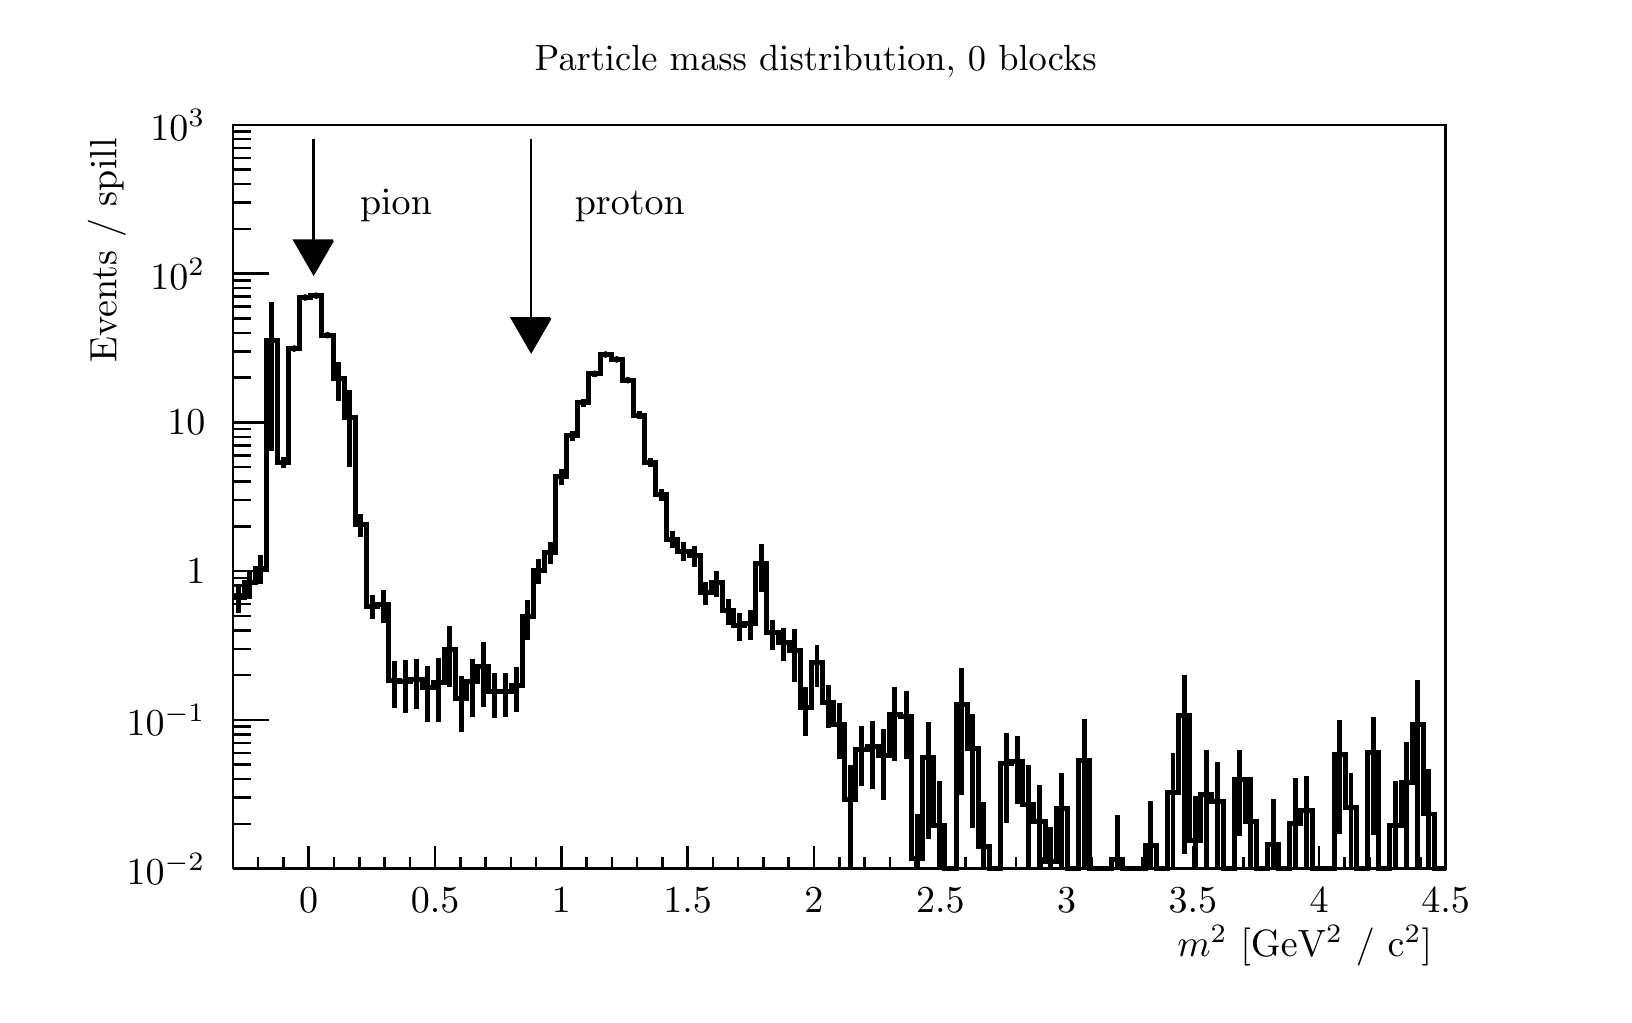
\begin{tikzpicture}
\pgfdeclareplotmark{cross} {
\pgfpathmoveto{\pgfpoint{-0.3\pgfplotmarksize}{\pgfplotmarksize}}
\pgfpathlineto{\pgfpoint{+0.3\pgfplotmarksize}{\pgfplotmarksize}}
\pgfpathlineto{\pgfpoint{+0.3\pgfplotmarksize}{0.3\pgfplotmarksize}}
\pgfpathlineto{\pgfpoint{+1\pgfplotmarksize}{0.3\pgfplotmarksize}}
\pgfpathlineto{\pgfpoint{+1\pgfplotmarksize}{-0.3\pgfplotmarksize}}
\pgfpathlineto{\pgfpoint{+0.3\pgfplotmarksize}{-0.3\pgfplotmarksize}}
\pgfpathlineto{\pgfpoint{+0.3\pgfplotmarksize}{-1.\pgfplotmarksize}}
\pgfpathlineto{\pgfpoint{-0.3\pgfplotmarksize}{-1.\pgfplotmarksize}}
\pgfpathlineto{\pgfpoint{-0.3\pgfplotmarksize}{-0.3\pgfplotmarksize}}
\pgfpathlineto{\pgfpoint{-1.\pgfplotmarksize}{-0.3\pgfplotmarksize}}
\pgfpathlineto{\pgfpoint{-1.\pgfplotmarksize}{0.3\pgfplotmarksize}}
\pgfpathlineto{\pgfpoint{-0.3\pgfplotmarksize}{0.3\pgfplotmarksize}}
\pgfpathclose
\pgfusepathqstroke
}
\pgfdeclareplotmark{cross*} {
\pgfpathmoveto{\pgfpoint{-0.3\pgfplotmarksize}{\pgfplotmarksize}}
\pgfpathlineto{\pgfpoint{+0.3\pgfplotmarksize}{\pgfplotmarksize}}
\pgfpathlineto{\pgfpoint{+0.3\pgfplotmarksize}{0.3\pgfplotmarksize}}
\pgfpathlineto{\pgfpoint{+1\pgfplotmarksize}{0.3\pgfplotmarksize}}
\pgfpathlineto{\pgfpoint{+1\pgfplotmarksize}{-0.3\pgfplotmarksize}}
\pgfpathlineto{\pgfpoint{+0.3\pgfplotmarksize}{-0.3\pgfplotmarksize}}
\pgfpathlineto{\pgfpoint{+0.3\pgfplotmarksize}{-1.\pgfplotmarksize}}
\pgfpathlineto{\pgfpoint{-0.3\pgfplotmarksize}{-1.\pgfplotmarksize}}
\pgfpathlineto{\pgfpoint{-0.3\pgfplotmarksize}{-0.3\pgfplotmarksize}}
\pgfpathlineto{\pgfpoint{-1.\pgfplotmarksize}{-0.3\pgfplotmarksize}}
\pgfpathlineto{\pgfpoint{-1.\pgfplotmarksize}{0.3\pgfplotmarksize}}
\pgfpathlineto{\pgfpoint{-0.3\pgfplotmarksize}{0.3\pgfplotmarksize}}
\pgfpathclose
\pgfusepathqfillstroke
}
\pgfdeclareplotmark{newstar} {
\pgfpathmoveto{\pgfqpoint{0pt}{\pgfplotmarksize}}
\pgfpathlineto{\pgfqpointpolar{44}{0.5\pgfplotmarksize}}
\pgfpathlineto{\pgfqpointpolar{18}{\pgfplotmarksize}}
\pgfpathlineto{\pgfqpointpolar{-20}{0.5\pgfplotmarksize}}
\pgfpathlineto{\pgfqpointpolar{-54}{\pgfplotmarksize}}
\pgfpathlineto{\pgfqpointpolar{-90}{0.5\pgfplotmarksize}}
\pgfpathlineto{\pgfqpointpolar{234}{\pgfplotmarksize}}
\pgfpathlineto{\pgfqpointpolar{198}{0.5\pgfplotmarksize}}
\pgfpathlineto{\pgfqpointpolar{162}{\pgfplotmarksize}}
\pgfpathlineto{\pgfqpointpolar{134}{0.5\pgfplotmarksize}}
\pgfpathclose
\pgfusepathqstroke
}
\pgfdeclareplotmark{newstar*} {
\pgfpathmoveto{\pgfqpoint{0pt}{\pgfplotmarksize}}
\pgfpathlineto{\pgfqpointpolar{44}{0.5\pgfplotmarksize}}
\pgfpathlineto{\pgfqpointpolar{18}{\pgfplotmarksize}}
\pgfpathlineto{\pgfqpointpolar{-20}{0.5\pgfplotmarksize}}
\pgfpathlineto{\pgfqpointpolar{-54}{\pgfplotmarksize}}
\pgfpathlineto{\pgfqpointpolar{-90}{0.5\pgfplotmarksize}}
\pgfpathlineto{\pgfqpointpolar{234}{\pgfplotmarksize}}
\pgfpathlineto{\pgfqpointpolar{198}{0.5\pgfplotmarksize}}
\pgfpathlineto{\pgfqpointpolar{162}{\pgfplotmarksize}}
\pgfpathlineto{\pgfqpointpolar{134}{0.5\pgfplotmarksize}}
\pgfpathclose
\pgfusepathqfillstroke
}
\definecolor{c}{rgb}{1,1,1};
\draw [color=c, fill=c] (0,0) rectangle (20,12.268);
\draw [color=c, fill=c] (2.6,1.59485) rectangle (18,11.0412);
\definecolor{c}{rgb}{0,0,0};
\draw [c,line width=0.9] (2.6,1.59485) -- (2.6,11.0412) -- (18,11.0412) -- (18,1.59485) -- (2.6,1.59485);
\definecolor{c}{rgb}{1,1,1};
\draw [color=c, fill=c] (2.6,1.59485) rectangle (18,11.0412);
\definecolor{c}{rgb}{0,0,0};
\draw [c,line width=0.9] (2.6,1.59485) -- (2.6,11.0412) -- (18,11.0412) -- (18,1.59485) -- (2.6,1.59485);
\draw [c,line width=1.8] (2.67064,4.83835) -- (2.67064,5.03878);
\draw [c,line width=1.8] (2.67064,5.03878) -- (2.67064,5.19974);
\foreach \P in {(2.67064,5.03878)}{\draw[mark options={color=c,fill=c},mark size=2.402402pt,mark=*,mark size=1pt] plot coordinates {\P};}
\draw [c,line width=1.8] (2.81193,5.02388) -- (2.81193,5.22754);
\draw [c,line width=1.8] (2.81193,5.22754) -- (2.81193,5.39056);
\foreach \P in {(2.81193,5.22754)}{\draw[mark options={color=c,fill=c},mark size=2.402402pt,mark=*,mark size=1pt] plot coordinates {\P};}
\draw [c,line width=1.8] (2.95321,5.20394) -- (2.95321,5.40915);
\draw [c,line width=1.8] (2.95321,5.40915) -- (2.95321,5.57317);
\foreach \P in {(2.95321,5.40915)}{\draw[mark options={color=c,fill=c},mark size=2.402402pt,mark=*,mark size=1pt] plot coordinates {\P};}
\draw [c,line width=1.8] (3.0945,6.89726) -- (3.0945,8.29886);
\draw [c,line width=1.8] (3.0945,8.29886) -- (3.0945,8.78967);
\foreach \P in {(3.0945,8.29886)}{\draw[mark options={color=c,fill=c},mark size=2.402402pt,mark=*,mark size=1pt] plot coordinates {\P};}
\draw [c,line width=1.8] (3.23578,6.67678) -- (3.23578,6.74991);
\draw [c,line width=1.8] (3.23578,6.74991) -- (3.23578,6.81705);
\foreach \P in {(3.23578,6.74991)}{\draw[mark options={color=c,fill=c},mark size=2.402402pt,mark=*,mark size=1pt] plot coordinates {\P};}
\draw [c,line width=1.8] (3.37706,8.16831) -- (3.37706,8.19982);
\draw [c,line width=1.8] (3.37706,8.19982) -- (3.37706,8.23016);
\foreach \P in {(3.37706,8.19982)}{\draw[mark options={color=c,fill=c},mark size=2.402402pt,mark=*,mark size=1pt] plot coordinates {\P};}
\draw [c,line width=1.8] (3.51835,8.82543) -- (3.51835,8.84804);
\draw [c,line width=1.8] (3.51835,8.84804) -- (3.51835,8.87003);
\foreach \P in {(3.51835,8.84804)}{\draw[mark options={color=c,fill=c},mark size=2.402402pt,mark=*,mark size=1pt] plot coordinates {\P};}
\draw [c,line width=1.8] (3.65963,8.85293) -- (3.65963,8.87184);
\draw [c,line width=1.8] (3.65963,8.87184) -- (3.65963,8.89033);
\foreach \P in {(3.65963,8.87184)}{\draw[mark options={color=c,fill=c},mark size=2.402402pt,mark=*,mark size=1pt] plot coordinates {\P};}
\draw [c,line width=1.8] (3.80092,8.34335) -- (3.80092,8.36936);
\draw [c,line width=1.8] (3.80092,8.36936) -- (3.80092,8.39457);
\foreach \P in {(3.80092,8.36936)}{\draw[mark options={color=c,fill=c},mark size=2.402402pt,mark=*,mark size=1pt] plot coordinates {\P};}
\draw [c,line width=1.8] (3.9422,7.53614) -- (3.9422,7.81768);
\draw [c,line width=1.8] (3.9422,7.81768) -- (3.9422,8.0269);
\foreach \P in {(3.9422,7.81768)}{\draw[mark options={color=c,fill=c},mark size=2.402402pt,mark=*,mark size=1pt] plot coordinates {\P};}
\draw [c,line width=1.8] (4.08349,6.6976) -- (4.08349,7.31909);
\draw [c,line width=1.8] (4.08349,7.31909) -- (4.08349,7.66863);
\foreach \P in {(4.08349,7.31909)}{\draw[mark options={color=c,fill=c},mark size=2.402402pt,mark=*,mark size=1pt] plot coordinates {\P};}
\draw [c,line width=1.8] (4.22477,5.80704) -- (4.22477,5.96886);
\draw [c,line width=1.8] (4.22477,5.96886) -- (4.22477,6.10395);
\foreach \P in {(4.22477,5.96886)}{\draw[mark options={color=c,fill=c},mark size=2.402402pt,mark=*,mark size=1pt] plot coordinates {\P};}
\draw [c,line width=1.8] (4.36606,4.76465) -- (4.36606,4.92769);
\draw [c,line width=1.8] (4.36606,4.92769) -- (4.36606,5.06364);
\foreach \P in {(4.36606,4.92769)}{\draw[mark options={color=c,fill=c},mark size=2.402402pt,mark=*,mark size=1pt] plot coordinates {\P};}
\draw [c,line width=1.8] (4.50734,4.70929) -- (4.50734,4.95225);
\draw [c,line width=1.8] (4.50734,4.95225) -- (4.50734,5.13946);
\foreach \P in {(4.50734,4.95225)}{\draw[mark options={color=c,fill=c},mark size=2.402402pt,mark=*,mark size=1pt] plot coordinates {\P};}
\draw [c,line width=1.8] (4.64862,3.63921) -- (4.64862,3.98727);
\draw [c,line width=1.8] (4.64862,3.98727) -- (4.64862,4.2309);
\foreach \P in {(4.64862,3.98727)}{\draw[mark options={color=c,fill=c},mark size=2.402402pt,mark=*,mark size=1pt] plot coordinates {\P};}
\draw [c,line width=1.8] (4.78991,3.57385) -- (4.78991,3.97748);
\draw [c,line width=1.8] (4.78991,3.97748) -- (4.78991,4.24682);
\foreach \P in {(4.78991,3.97748)}{\draw[mark options={color=c,fill=c},mark size=2.402402pt,mark=*,mark size=1pt] plot coordinates {\P};}
\draw [c,line width=1.8] (4.93119,3.61791) -- (4.93119,4.00227);
\draw [c,line width=1.8] (4.93119,4.00227) -- (4.93119,4.26298);
\foreach \P in {(4.93119,4.00227)}{\draw[mark options={color=c,fill=c},mark size=2.402402pt,mark=*,mark size=1pt] plot coordinates {\P};}
\draw [c,line width=1.8] (5.07248,3.45883) -- (5.07248,3.89031);
\draw [c,line width=1.8] (5.07248,3.89031) -- (5.07248,4.17163);
\foreach \P in {(5.07248,3.89031)}{\draw[mark options={color=c,fill=c},mark size=2.402402pt,mark=*,mark size=1pt] plot coordinates {\P};}
\draw [c,line width=1.8] (5.21376,3.4566) -- (5.21376,3.96471);
\draw [c,line width=1.8] (5.21376,3.96471) -- (5.21376,4.27615);
\foreach \P in {(5.21376,3.96471)}{\draw[mark options={color=c,fill=c},mark size=2.402402pt,mark=*,mark size=1pt] plot coordinates {\P};}
\draw [c,line width=1.8] (5.35505,3.89726) -- (5.35505,4.37437);
\draw [c,line width=1.8] (5.35505,4.37437) -- (5.35505,4.67409);
\foreach \P in {(5.35505,4.37437)}{\draw[mark options={color=c,fill=c},mark size=2.402402pt,mark=*,mark size=1pt] plot coordinates {\P};}
\draw [c,line width=1.8] (5.49633,3.32673) -- (5.49633,3.75962);
\draw [c,line width=1.8] (5.49633,3.75962) -- (5.49633,4.04152);
\foreach \P in {(5.49633,3.75962)}{\draw[mark options={color=c,fill=c},mark size=2.402402pt,mark=*,mark size=1pt] plot coordinates {\P};}
\draw [c,line width=1.8] (5.63761,3.52578) -- (5.63761,3.96588);
\draw [c,line width=1.8] (5.63761,3.96588) -- (5.63761,4.25079);
\foreach \P in {(5.63761,3.96588)}{\draw[mark options={color=c,fill=c},mark size=2.402402pt,mark=*,mark size=1pt] plot coordinates {\P};}
\draw [c,line width=1.8] (5.7789,3.65191) -- (5.7789,4.16508);
\draw [c,line width=1.8] (5.7789,4.16508) -- (5.7789,4.47837);
\foreach \P in {(5.7789,4.16508)}{\draw[mark options={color=c,fill=c},mark size=2.402402pt,mark=*,mark size=1pt] plot coordinates {\P};}
\draw [c,line width=1.8] (5.92018,3.50311) -- (5.92018,3.84313);
\draw [c,line width=1.8] (5.92018,3.84313) -- (5.92018,4.08282);
\foreach \P in {(5.92018,3.84313)}{\draw[mark options={color=c,fill=c},mark size=2.402402pt,mark=*,mark size=1pt] plot coordinates {\P};}
\draw [c,line width=1.8] (6.06147,3.52606) -- (6.06147,3.84806);
\draw [c,line width=1.8] (6.06147,3.84806) -- (6.06147,4.07871);
\foreach \P in {(6.06147,3.84806)}{\draw[mark options={color=c,fill=c},mark size=2.402402pt,mark=*,mark size=1pt] plot coordinates {\P};}
\draw [c,line width=1.8] (6.20275,3.58333) -- (6.20275,3.91725);
\draw [c,line width=1.8] (6.20275,3.91725) -- (6.20275,4.15391);
\foreach \P in {(6.20275,3.91725)}{\draw[mark options={color=c,fill=c},mark size=2.402402pt,mark=*,mark size=1pt] plot coordinates {\P};}
\draw [c,line width=1.8] (6.34404,4.49729) -- (6.34404,4.79092);
\draw [c,line width=1.8] (6.34404,4.79092) -- (6.34404,5.00671);
\foreach \P in {(6.34404,4.79092)}{\draw[mark options={color=c,fill=c},mark size=2.402402pt,mark=*,mark size=1pt] plot coordinates {\P};}
\draw [c,line width=1.8] (6.48532,5.21427) -- (6.48532,5.38521);
\draw [c,line width=1.8] (6.48532,5.38521) -- (6.48532,5.52661);
\foreach \P in {(6.48532,5.38521)}{\draw[mark options={color=c,fill=c},mark size=2.402402pt,mark=*,mark size=1pt] plot coordinates {\P};}
\draw [c,line width=1.8] (6.62661,5.45876) -- (6.62661,5.60996);
\draw [c,line width=1.8] (6.62661,5.60996) -- (6.62661,5.73757);
\foreach \P in {(6.62661,5.60996)}{\draw[mark options={color=c,fill=c},mark size=2.402402pt,mark=*,mark size=1pt] plot coordinates {\P};}
\draw [c,line width=1.8] (6.76789,6.46087) -- (6.76789,6.56975);
\draw [c,line width=1.8] (6.76789,6.56975) -- (6.76789,6.66587);
\foreach \P in {(6.76789,6.56975)}{\draw[mark options={color=c,fill=c},mark size=2.402402pt,mark=*,mark size=1pt] plot coordinates {\P};}
\draw [c,line width=1.8] (6.90917,7.02428) -- (6.90917,7.09333);
\draw [c,line width=1.8] (6.90917,7.09333) -- (6.90917,7.15701);
\foreach \P in {(6.90917,7.09333)}{\draw[mark options={color=c,fill=c},mark size=2.402402pt,mark=*,mark size=1pt] plot coordinates {\P};}
\draw [c,line width=1.8] (7.05046,7.46269) -- (7.05046,7.51223);
\draw [c,line width=1.8] (7.05046,7.51223) -- (7.05046,7.55895);
\foreach \P in {(7.05046,7.51223)}{\draw[mark options={color=c,fill=c},mark size=2.402402pt,mark=*,mark size=1pt] plot coordinates {\P};}
\draw [c,line width=1.8] (7.19174,7.84097) -- (7.19174,7.87899);
\draw [c,line width=1.8] (7.19174,7.87899) -- (7.19174,7.91532);
\foreach \P in {(7.19174,7.87899)}{\draw[mark options={color=c,fill=c},mark size=2.402402pt,mark=*,mark size=1pt] plot coordinates {\P};}
\draw [c,line width=1.8] (7.33303,8.08654) -- (7.33303,8.12401);
\draw [c,line width=1.8] (7.33303,8.12401) -- (7.33303,8.15984);
\foreach \P in {(7.33303,8.12401)}{\draw[mark options={color=c,fill=c},mark size=2.402402pt,mark=*,mark size=1pt] plot coordinates {\P};}
\draw [c,line width=1.8] (7.47431,8.03213) -- (7.47431,8.06216);
\draw [c,line width=1.8] (7.47431,8.06216) -- (7.47431,8.09112);
\foreach \P in {(7.47431,8.06216)}{\draw[mark options={color=c,fill=c},mark size=2.402402pt,mark=*,mark size=1pt] plot coordinates {\P};}
\draw [c,line width=1.8] (7.6156,7.76525) -- (7.6156,7.79819);
\draw [c,line width=1.8] (7.6156,7.79819) -- (7.6156,7.82986);
\foreach \P in {(7.6156,7.79819)}{\draw[mark options={color=c,fill=c},mark size=2.402402pt,mark=*,mark size=1pt] plot coordinates {\P};}
\draw [c,line width=1.8] (7.75688,7.30594) -- (7.75688,7.35538);
\draw [c,line width=1.8] (7.75688,7.35538) -- (7.75688,7.40201);
\foreach \P in {(7.75688,7.35538)}{\draw[mark options={color=c,fill=c},mark size=2.402402pt,mark=*,mark size=1pt] plot coordinates {\P};}
\draw [c,line width=1.8] (7.89817,6.6923) -- (7.89817,6.75283);
\draw [c,line width=1.8] (7.89817,6.75283) -- (7.89817,6.8092);
\foreach \P in {(7.89817,6.75283)}{\draw[mark options={color=c,fill=c},mark size=2.402402pt,mark=*,mark size=1pt] plot coordinates {\P};}
\draw [c,line width=1.8] (8.03945,6.26213) -- (8.03945,6.34253);
\draw [c,line width=1.8] (8.03945,6.34253) -- (8.03945,6.41575);
\foreach \P in {(8.03945,6.34253)}{\draw[mark options={color=c,fill=c},mark size=2.402402pt,mark=*,mark size=1pt] plot coordinates {\P};}
\draw [c,line width=1.8] (8.18073,5.66331) -- (8.18073,5.77852);
\draw [c,line width=1.8] (8.18073,5.77852) -- (8.18073,5.87952);
\foreach \P in {(8.18073,5.77852)}{\draw[mark options={color=c,fill=c},mark size=2.402402pt,mark=*,mark size=1pt] plot coordinates {\P};}
\draw [c,line width=1.8] (8.32202,5.49675) -- (8.32202,5.62806);
\draw [c,line width=1.8] (8.32202,5.62806) -- (8.32202,5.74122);
\foreach \P in {(8.32202,5.62806)}{\draw[mark options={color=c,fill=c},mark size=2.402402pt,mark=*,mark size=1pt] plot coordinates {\P};}
\draw [c,line width=1.8] (8.4633,5.4312) -- (8.4633,5.56853);
\draw [c,line width=1.8] (8.4633,5.56853) -- (8.4633,5.68614);
\foreach \P in {(8.4633,5.56853)}{\draw[mark options={color=c,fill=c},mark size=2.402402pt,mark=*,mark size=1pt] plot coordinates {\P};}
\draw [c,line width=1.8] (8.60459,4.93703) -- (8.60459,5.10131);
\draw [c,line width=1.8] (8.60459,5.10131) -- (8.60459,5.23811);
\foreach \P in {(8.60459,5.10131)}{\draw[mark options={color=c,fill=c},mark size=2.402402pt,mark=*,mark size=1pt] plot coordinates {\P};}
\draw [c,line width=1.8] (8.74587,5.04831) -- (8.74587,5.225);
\draw [c,line width=1.8] (8.74587,5.225) -- (8.74587,5.3703);
\foreach \P in {(8.74587,5.225)}{\draw[mark options={color=c,fill=c},mark size=2.402402pt,mark=*,mark size=1pt] plot coordinates {\P};}
\draw [c,line width=1.8] (8.88716,4.69464) -- (8.88716,4.87042);
\draw [c,line width=1.8] (8.88716,4.87042) -- (8.88716,5.01511);
\foreach \P in {(8.88716,4.87042)}{\draw[mark options={color=c,fill=c},mark size=2.402402pt,mark=*,mark size=1pt] plot coordinates {\P};}
\draw [c,line width=1.8] (9.02844,4.4874) -- (9.02844,4.68535);
\draw [c,line width=1.8] (9.02844,4.68535) -- (9.02844,4.8447);
\foreach \P in {(9.02844,4.68535)}{\draw[mark options={color=c,fill=c},mark size=2.402402pt,mark=*,mark size=1pt] plot coordinates {\P};}
\draw [c,line width=1.8] (9.16972,4.49569) -- (9.16972,4.71155);
\draw [c,line width=1.8] (9.16972,4.71155) -- (9.16972,4.88229);
\foreach \P in {(9.16972,4.71155)}{\draw[mark options={color=c,fill=c},mark size=2.402402pt,mark=*,mark size=1pt] plot coordinates {\P};}
\draw [c,line width=1.8] (9.31101,5.10451) -- (9.31101,5.46375);
\draw [c,line width=1.8] (9.31101,5.46375) -- (9.31101,5.71275);
\foreach \P in {(9.31101,5.46375)}{\draw[mark options={color=c,fill=c},mark size=2.402402pt,mark=*,mark size=1pt] plot coordinates {\P};}
\draw [c,line width=1.8] (9.45229,4.3732) -- (9.45229,4.58756);
\draw [c,line width=1.8] (9.45229,4.58756) -- (9.45229,4.75736);
\foreach \P in {(9.45229,4.58756)}{\draw[mark options={color=c,fill=c},mark size=2.402402pt,mark=*,mark size=1pt] plot coordinates {\P};}
\draw [c,line width=1.8] (9.59358,4.23243) -- (9.59358,4.46821);
\draw [c,line width=1.8] (9.59358,4.46821) -- (9.59358,4.65113);
\foreach \P in {(9.59358,4.46821)}{\draw[mark options={color=c,fill=c},mark size=2.402402pt,mark=*,mark size=1pt] plot coordinates {\P};}
\draw [c,line width=1.8] (9.73486,3.95946) -- (9.73486,4.37117);
\draw [c,line width=1.8] (9.73486,4.37117) -- (9.73486,4.64405);
\foreach \P in {(9.73486,4.37117)}{\draw[mark options={color=c,fill=c},mark size=2.402402pt,mark=*,mark size=1pt] plot coordinates {\P};}
\draw [c,line width=1.8] (9.87615,3.27572) -- (9.87615,3.64567);
\draw [c,line width=1.8] (9.87615,3.64567) -- (9.87615,3.89972);
\foreach \P in {(9.87615,3.64567)}{\draw[mark options={color=c,fill=c},mark size=2.402402pt,mark=*,mark size=1pt] plot coordinates {\P};}
\draw [c,line width=1.8] (10.0174,3.90501) -- (10.0174,4.21346);
\draw [c,line width=1.8] (10.0174,4.21346) -- (10.0174,4.43711);
\foreach \P in {(10.0174,4.21346)}{\draw[mark options={color=c,fill=c},mark size=2.402402pt,mark=*,mark size=1pt] plot coordinates {\P};}
\draw [c,line width=1.8] (10.1587,3.37914) -- (10.1587,3.69867);
\draw [c,line width=1.8] (10.1587,3.69867) -- (10.1587,3.92806);
\foreach \P in {(10.1587,3.69867)}{\draw[mark options={color=c,fill=c},mark size=2.402402pt,mark=*,mark size=1pt] plot coordinates {\P};}
\draw [c,line width=1.8] (10.3,2.98811) -- (10.3,3.42043);
\draw [c,line width=1.8] (10.3,3.42043) -- (10.3,3.70209);
\foreach \P in {(10.3,3.42043)}{\draw[mark options={color=c,fill=c},mark size=2.402402pt,mark=*,mark size=1pt] plot coordinates {\P};}
\draw [c,line width=1.8] (10.4413,1.59485) -- (10.4413,2.46862);
\draw [c,line width=1.8] (10.4413,2.46862) -- (10.4413,2.90743);
\foreach \P in {(10.4413,2.46862)}{\draw[mark options={color=c,fill=c},mark size=2.402402pt,mark=*,mark size=1pt] plot coordinates {\P};}
\draw [c,line width=1.8] (10.5826,2.64925) -- (10.5826,3.11372);
\draw [c,line width=1.8] (10.5826,3.11372) -- (10.5826,3.40849);
\foreach \P in {(10.5826,3.11372)}{\draw[mark options={color=c,fill=c},mark size=2.402402pt,mark=*,mark size=1pt] plot coordinates {\P};}
\draw [c,line width=1.8] (10.7239,2.6029) -- (10.7239,3.14556);
\draw [c,line width=1.8] (10.7239,3.14556) -- (10.7239,3.46937);
\foreach \P in {(10.7239,3.14556)}{\draw[mark options={color=c,fill=c},mark size=2.402402pt,mark=*,mark size=1pt] plot coordinates {\P};}
\draw [c,line width=1.8] (10.8651,2.462) -- (10.8651,3.03474);
\draw [c,line width=1.8] (10.8651,3.03474) -- (10.8651,3.36876);
\foreach \P in {(10.8651,3.03474)}{\draw[mark options={color=c,fill=c},mark size=2.402402pt,mark=*,mark size=1pt] plot coordinates {\P};}
\draw [c,line width=1.8] (11.0064,2.9672) -- (11.0064,3.55656);
\draw [c,line width=1.8] (11.0064,3.55656) -- (11.0064,3.896);
\foreach \P in {(11.0064,3.55656)}{\draw[mark options={color=c,fill=c},mark size=2.402402pt,mark=*,mark size=1pt] plot coordinates {\P};}
\draw [c,line width=1.8] (11.1477,2.98208) -- (11.1477,3.52359);
\draw [c,line width=1.8] (11.1477,3.52359) -- (11.1477,3.847);
\foreach \P in {(11.1477,3.52359)}{\draw[mark options={color=c,fill=c},mark size=2.402402pt,mark=*,mark size=1pt] plot coordinates {\P};}
\draw [c,line width=1.8] (11.289,1.59485) -- (11.289,1.72064);
\draw [c,line width=1.8] (11.289,1.72064) -- (11.289,2.28937);
\foreach \P in {(11.289,1.72064)}{\draw[mark options={color=c,fill=c},mark size=2.402402pt,mark=*,mark size=1pt] plot coordinates {\P};}
\draw [c,line width=1.8] (11.4303,1.97434) -- (11.4303,3.01);
\draw [c,line width=1.8] (11.4303,3.01) -- (11.4303,3.45354);
\foreach \P in {(11.4303,3.01)}{\draw[mark options={color=c,fill=c},mark size=2.402402pt,mark=*,mark size=1pt] plot coordinates {\P};}
\draw [c,line width=1.8] (11.5716,1.59485) -- (11.5716,2.13924);
\draw [c,line width=1.8] (11.5716,2.13924) -- (11.5716,2.70797);
\foreach \P in {(11.5716,2.13924)}{\draw[mark options={color=c,fill=c},mark size=2.402402pt,mark=*,mark size=1pt] plot coordinates {\P};}
\draw [c,line width=1.8] (11.8541,2.52934) -- (11.8541,3.6822);
\draw [c,line width=1.8] (11.8541,3.6822) -- (11.8541,4.14354);
\foreach \P in {(11.8541,3.6822)}{\draw[mark options={color=c,fill=c},mark size=2.402402pt,mark=*,mark size=1pt] plot coordinates {\P};}
\draw [c,line width=1.8] (11.9954,2.10703) -- (11.9954,3.12444);
\draw [c,line width=1.8] (11.9954,3.12444) -- (11.9954,3.56493);
\foreach \P in {(11.9954,3.12444)}{\draw[mark options={color=c,fill=c},mark size=2.402402pt,mark=*,mark size=1pt] plot coordinates {\P};}
\draw [c,line width=1.8] (12.1367,1.59485) -- (12.1367,1.87338);
\draw [c,line width=1.8] (12.1367,1.87338) -- (12.1367,2.44211);
\foreach \P in {(12.1367,1.87338)}{\draw[mark options={color=c,fill=c},mark size=2.402402pt,mark=*,mark size=1pt] plot coordinates {\P};}
\draw [c,line width=1.8] (12.4193,2.17688) -- (12.4193,2.93019);
\draw [c,line width=1.8] (12.4193,2.93019) -- (12.4193,3.3162);
\foreach \P in {(12.4193,2.93019)}{\draw[mark options={color=c,fill=c},mark size=2.402402pt,mark=*,mark size=1pt] plot coordinates {\P};}
\draw [c,line width=1.8] (12.5606,2.41698) -- (12.5606,2.9556);
\draw [c,line width=1.8] (12.5606,2.9556) -- (12.5606,3.278);
\foreach \P in {(12.5606,2.9556)}{\draw[mark options={color=c,fill=c},mark size=2.402402pt,mark=*,mark size=1pt] plot coordinates {\P};}
\draw [c,line width=1.8] (12.7018,1.59485) -- (12.7018,2.41357);
\draw [c,line width=1.8] (12.7018,2.41357) -- (12.7018,2.90521);
\foreach \P in {(12.7018,2.41357)}{\draw[mark options={color=c,fill=c},mark size=2.402402pt,mark=*,mark size=1pt] plot coordinates {\P};}
\draw [c,line width=1.8] (12.8431,1.59485) -- (12.8431,2.19842);
\draw [c,line width=1.8] (12.8431,2.19842) -- (12.8431,2.65912);
\foreach \P in {(12.8431,2.19842)}{\draw[mark options={color=c,fill=c},mark size=2.402402pt,mark=*,mark size=1pt] plot coordinates {\P};}
\draw [c,line width=1.8] (12.9844,1.59485) -- (12.9844,1.6838);
\draw [c,line width=1.8] (12.9844,1.6838) -- (12.9844,2.12472);
\foreach \P in {(12.9844,1.6838)}{\draw[mark options={color=c,fill=c},mark size=2.402402pt,mark=*,mark size=1pt] plot coordinates {\P};}
\draw [c,line width=1.8] (13.1257,1.59485) -- (13.1257,2.36408);
\draw [c,line width=1.8] (13.1257,2.36408) -- (13.1257,2.8032);
\foreach \P in {(13.1257,2.36408)}{\draw[mark options={color=c,fill=c},mark size=2.402402pt,mark=*,mark size=1pt] plot coordinates {\P};}
\draw [c,line width=1.8] (13.4083,1.59485) -- (13.4083,2.96797);
\draw [c,line width=1.8] (13.4083,2.96797) -- (13.4083,3.49089);
\foreach \P in {(13.4083,2.96797)}{\draw[mark options={color=c,fill=c},mark size=2.402402pt,mark=*,mark size=1pt] plot coordinates {\P};}
\draw [c,line width=1.8] (13.8321,1.59485) -- (13.8321,1.70796);
\draw [c,line width=1.8] (13.8321,1.70796) -- (13.8321,2.27669);
\foreach \P in {(13.8321,1.70796)}{\draw[mark options={color=c,fill=c},mark size=2.402402pt,mark=*,mark size=1pt] plot coordinates {\P};}
\draw [c,line width=1.8] (14.256,1.59485) -- (14.256,1.88635);
\draw [c,line width=1.8] (14.256,1.88635) -- (14.256,2.45508);
\foreach \P in {(14.256,1.88635)}{\draw[mark options={color=c,fill=c},mark size=2.402402pt,mark=*,mark size=1pt] plot coordinates {\P};}
\draw [c,line width=1.8] (14.5385,1.59485) -- (14.5385,2.56214);
\draw [c,line width=1.8] (14.5385,2.56214) -- (14.5385,3.05869);
\foreach \P in {(14.5385,2.56214)}{\draw[mark options={color=c,fill=c},mark size=2.402402pt,mark=*,mark size=1pt] plot coordinates {\P};}
\draw [c,line width=1.8] (14.6798,1.77804) -- (14.6798,3.53455);
\draw [c,line width=1.8] (14.6798,3.53455) -- (14.6798,4.05358);
\foreach \P in {(14.6798,3.53455)}{\draw[mark options={color=c,fill=c},mark size=2.402402pt,mark=*,mark size=1pt] plot coordinates {\P};}
\draw [c,line width=1.8] (14.8211,1.59485) -- (14.8211,1.95322);
\draw [c,line width=1.8] (14.8211,1.95322) -- (14.8211,2.52195);
\foreach \P in {(14.8211,1.95322)}{\draw[mark options={color=c,fill=c},mark size=2.402402pt,mark=*,mark size=1pt] plot coordinates {\P};}
\draw [c,line width=1.8] (14.9624,1.59485) -- (14.9624,2.53325);
\draw [c,line width=1.8] (14.9624,2.53325) -- (14.9624,3.10198);
\foreach \P in {(14.9624,2.53325)}{\draw[mark options={color=c,fill=c},mark size=2.402402pt,mark=*,mark size=1pt] plot coordinates {\P};}
\draw [c,line width=1.8] (15.1037,1.59485) -- (15.1037,2.44678);
\draw [c,line width=1.8] (15.1037,2.44678) -- (15.1037,2.94849);
\foreach \P in {(15.1037,2.44678)}{\draw[mark options={color=c,fill=c},mark size=2.402402pt,mark=*,mark size=1pt] plot coordinates {\P};}
\draw [c,line width=1.8] (15.3862,2.00303) -- (15.3862,2.72073);
\draw [c,line width=1.8] (15.3862,2.72073) -- (15.3862,3.09761);
\foreach \P in {(15.3862,2.72073)}{\draw[mark options={color=c,fill=c},mark size=2.402402pt,mark=*,mark size=1pt] plot coordinates {\P};}
\draw [c,line width=1.8] (15.5275,1.59485) -- (15.5275,2.18974);
\draw [c,line width=1.8] (15.5275,2.18974) -- (15.5275,2.75847);
\foreach \P in {(15.5275,2.18974)}{\draw[mark options={color=c,fill=c},mark size=2.402402pt,mark=*,mark size=1pt] plot coordinates {\P};}
\draw [c,line width=1.8] (15.8101,1.59485) -- (15.8101,1.90579);
\draw [c,line width=1.8] (15.8101,1.90579) -- (15.8101,2.47452);
\foreach \P in {(15.8101,1.90579)}{\draw[mark options={color=c,fill=c},mark size=2.402402pt,mark=*,mark size=1pt] plot coordinates {\P};}
\draw [c,line width=1.8] (16.0927,1.59485) -- (16.0927,2.17394);
\draw [c,line width=1.8] (16.0927,2.17394) -- (16.0927,2.74267);
\foreach \P in {(16.0927,2.17394)}{\draw[mark options={color=c,fill=c},mark size=2.402402pt,mark=*,mark size=1pt] plot coordinates {\P};}
\draw [c,line width=1.8] (16.2339,1.59485) -- (16.2339,2.33531);
\draw [c,line width=1.8] (16.2339,2.33531) -- (16.2339,2.77492);
\foreach \P in {(16.2339,2.33531)}{\draw[mark options={color=c,fill=c},mark size=2.402402pt,mark=*,mark size=1pt] plot coordinates {\P};}
\draw [c,line width=1.8] (16.6578,2.03451) -- (16.6578,3.04204);
\draw [c,line width=1.8] (16.6578,3.04204) -- (16.6578,3.48085);
\foreach \P in {(16.6578,3.04204)}{\draw[mark options={color=c,fill=c},mark size=2.402402pt,mark=*,mark size=1pt] plot coordinates {\P};}
\draw [c,line width=1.8] (16.7991,1.59485) -- (16.7991,2.36988);
\draw [c,line width=1.8] (16.7991,2.36988) -- (16.7991,2.81071);
\foreach \P in {(16.7991,2.36988)}{\draw[mark options={color=c,fill=c},mark size=2.402402pt,mark=*,mark size=1pt] plot coordinates {\P};}
\draw [c,line width=1.8] (17.0817,2.02663) -- (17.0817,3.07539);
\draw [c,line width=1.8] (17.0817,3.07539) -- (17.0817,3.52107);
\foreach \P in {(17.0817,3.07539)}{\draw[mark options={color=c,fill=c},mark size=2.402402pt,mark=*,mark size=1pt] plot coordinates {\P};}
\draw [c,line width=1.8] (17.3642,1.59485) -- (17.3642,2.13924);
\draw [c,line width=1.8] (17.3642,2.13924) -- (17.3642,2.70797);
\foreach \P in {(17.3642,2.13924)}{\draw[mark options={color=c,fill=c},mark size=2.402402pt,mark=*,mark size=1pt] plot coordinates {\P};}
\draw [c,line width=1.8] (17.5055,1.59485) -- (17.5055,2.6833);
\draw [c,line width=1.8] (17.5055,2.6833) -- (17.5055,3.19738);
\foreach \P in {(17.5055,2.6833)}{\draw[mark options={color=c,fill=c},mark size=2.402402pt,mark=*,mark size=1pt] plot coordinates {\P};}
\draw [c,line width=1.8] (17.6468,1.59485) -- (17.6468,3.42339);
\draw [c,line width=1.8] (17.6468,3.42339) -- (17.6468,3.99212);
\foreach \P in {(17.6468,3.42339)}{\draw[mark options={color=c,fill=c},mark size=2.402402pt,mark=*,mark size=1pt] plot coordinates {\P};}
\draw [c,line width=1.8] (17.7881,1.59485) -- (17.7881,2.28866);
\draw [c,line width=1.8] (17.7881,2.28866) -- (17.7881,2.85738);
\foreach \P in {(17.7881,2.28866)}{\draw[mark options={color=c,fill=c},mark size=2.402402pt,mark=*,mark size=1pt] plot coordinates {\P};}
\draw [c,line width=1.8] (2.6,5.03878) -- (2.74128,5.03878) -- (2.74128,5.22754) -- (2.88257,5.22754) -- (2.88257,5.40915) -- (3.02385,5.40915) -- (3.02385,8.29886) -- (3.16514,8.29886) -- (3.16514,6.74991) -- (3.30642,6.74991) -- (3.30642,8.19982)
 -- (3.44771,8.19982) -- (3.44771,8.84804) -- (3.58899,8.84804) -- (3.58899,8.87184) -- (3.73028,8.87184) -- (3.73028,8.36936) -- (3.87156,8.36936) -- (3.87156,7.81768) -- (4.01284,7.81768) -- (4.01284,7.31909) -- (4.15413,7.31909) --
 (4.15413,5.96886) -- (4.29541,5.96886) -- (4.29541,4.92769) -- (4.4367,4.92769) -- (4.4367,4.95225) -- (4.57798,4.95225) -- (4.57798,3.98727) -- (4.71927,3.98727) -- (4.71927,3.97748) -- (4.86055,3.97748) -- (4.86055,4.00227) -- (5.00183,4.00227) --
 (5.00183,3.89031) -- (5.14312,3.89031) -- (5.14312,3.96471) -- (5.2844,3.96471) -- (5.2844,4.37437) -- (5.42569,4.37437) -- (5.42569,3.75962) -- (5.56697,3.75962) -- (5.56697,3.96588) -- (5.70826,3.96588) -- (5.70826,4.16508) -- (5.84954,4.16508) --
 (5.84954,3.84313) -- (5.99083,3.84313) -- (5.99083,3.84806) -- (6.13211,3.84806) -- (6.13211,3.91725) -- (6.27339,3.91725) -- (6.27339,4.79092) -- (6.41468,4.79092) -- (6.41468,5.38521) -- (6.55596,5.38521) -- (6.55596,5.60996) -- (6.69725,5.60996)
 -- (6.69725,6.56975) -- (6.83853,6.56975) -- (6.83853,7.09333) -- (6.97982,7.09333) -- (6.97982,7.51223) -- (7.1211,7.51223) -- (7.1211,7.87899) -- (7.26239,7.87899) -- (7.26239,8.12401) -- (7.40367,8.12401) -- (7.40367,8.06216) -- (7.54495,8.06216)
 -- (7.54495,7.79819) -- (7.68624,7.79819) -- (7.68624,7.35538) -- (7.82752,7.35538) -- (7.82752,6.75283) -- (7.96881,6.75283) -- (7.96881,6.34253) -- (8.11009,6.34253) -- (8.11009,5.77852) -- (8.25138,5.77852) -- (8.25138,5.62806) --
 (8.39266,5.62806) -- (8.39266,5.56853) -- (8.53395,5.56853) -- (8.53395,5.10131) -- (8.67523,5.10131) -- (8.67523,5.225) -- (8.81651,5.225) -- (8.81651,4.87042) -- (8.9578,4.87042) -- (8.9578,4.68535) -- (9.09908,4.68535) -- (9.09908,4.71155) --
 (9.24037,4.71155) -- (9.24037,5.46375) -- (9.38165,5.46375) -- (9.38165,4.58756) -- (9.52294,4.58756) -- (9.52294,4.46821) -- (9.66422,4.46821) -- (9.66422,4.37117) -- (9.8055,4.37117) -- (9.8055,3.64567) -- (9.94679,3.64567) -- (9.94679,4.21346) --
 (10.0881,4.21346) -- (10.0881,3.69867) -- (10.2294,3.69867) -- (10.2294,3.42043) -- (10.3706,3.42043) -- (10.3706,2.46862) -- (10.5119,2.46862) -- (10.5119,3.11372) -- (10.6532,3.11372) -- (10.6532,3.14556) -- (10.7945,3.14556) -- (10.7945,3.03474)
 -- (10.9358,3.03474) -- (10.9358,3.55656) -- (11.0771,3.55656) -- (11.0771,3.52359) -- (11.2183,3.52359) -- (11.2183,1.72064) -- (11.3596,1.72064) -- (11.3596,3.01) -- (11.5009,3.01) -- (11.5009,2.13924) -- (11.6422,2.13924) -- (11.6422,1.59485) --
 (11.7835,1.59485) -- (11.7835,3.6822) -- (11.9248,3.6822) -- (11.9248,3.12444) -- (12.0661,3.12444) -- (12.0661,1.87338) -- (12.2073,1.87338) -- (12.2073,1.59485) -- (12.3486,1.59485) -- (12.3486,2.93019) -- (12.4899,2.93019) -- (12.4899,2.9556) --
 (12.6312,2.9556) -- (12.6312,2.41357) -- (12.7725,2.41357) -- (12.7725,2.19842) -- (12.9138,2.19842) -- (12.9138,1.6838) -- (13.055,1.6838) -- (13.055,2.36408) -- (13.1963,2.36408) -- (13.1963,1.59485) -- (13.3376,1.59485) -- (13.3376,2.96797) --
 (13.4789,2.96797) -- (13.4789,1.59485) -- (13.6202,1.59485) -- (13.6202,1.59485) -- (13.7615,1.59485) -- (13.7615,1.70796) -- (13.9028,1.70796) -- (13.9028,1.59485) -- (14.044,1.59485) -- (14.044,1.59485) -- (14.1853,1.59485) -- (14.1853,1.88635) --
 (14.3266,1.88635) -- (14.3266,1.59485) -- (14.4679,1.59485) -- (14.4679,2.56214) -- (14.6092,2.56214) -- (14.6092,3.53455) -- (14.7505,3.53455) -- (14.7505,1.95322) -- (14.8917,1.95322) -- (14.8917,2.53325) -- (15.033,2.53325) -- (15.033,2.44678) --
 (15.1743,2.44678) -- (15.1743,1.59485) -- (15.3156,1.59485) -- (15.3156,2.72073) -- (15.4569,2.72073) -- (15.4569,2.18974) -- (15.5982,2.18974) -- (15.5982,1.59485) -- (15.7394,1.59485) -- (15.7394,1.90579) -- (15.8807,1.90579) -- (15.8807,1.59485)
 -- (16.022,1.59485) -- (16.022,2.17394) -- (16.1633,2.17394) -- (16.1633,2.33531) -- (16.3046,2.33531) -- (16.3046,1.59485) -- (16.4459,1.59485) -- (16.4459,1.59485) -- (16.5872,1.59485) -- (16.5872,3.04204) -- (16.7284,3.04204) -- (16.7284,2.36988)
 -- (16.8697,2.36988) -- (16.8697,1.59485) -- (17.011,1.59485) -- (17.011,3.07539) -- (17.1523,3.07539) -- (17.1523,1.59485) -- (17.2936,1.59485) -- (17.2936,2.13924) -- (17.4349,2.13924) -- (17.4349,2.6833) -- (17.5761,2.6833) -- (17.5761,3.42339)
 -- (17.7174,3.42339) -- (17.7174,2.28866) -- (17.8587,2.28866) -- (17.8587,1.59485) -- (18,1.59485);
\draw [c,line width=0.9] (2.6,1.59485) -- (18,1.59485);
\draw [c,line width=0.9] (3.5625,1.87824) -- (3.5625,1.59485);
\draw [c,line width=0.9] (3.88333,1.73654) -- (3.88333,1.59485);
\draw [c,line width=0.9] (4.20417,1.73654) -- (4.20417,1.59485);
\draw [c,line width=0.9] (4.525,1.73654) -- (4.525,1.59485);
\draw [c,line width=0.9] (4.84583,1.73654) -- (4.84583,1.59485);
\draw [c,line width=0.9] (5.16667,1.87824) -- (5.16667,1.59485);
\draw [c,line width=0.9] (5.4875,1.73654) -- (5.4875,1.59485);
\draw [c,line width=0.9] (5.80833,1.73654) -- (5.80833,1.59485);
\draw [c,line width=0.9] (6.12917,1.73654) -- (6.12917,1.59485);
\draw [c,line width=0.9] (6.45,1.73654) -- (6.45,1.59485);
\draw [c,line width=0.9] (6.77083,1.87824) -- (6.77083,1.59485);
\draw [c,line width=0.9] (7.09167,1.73654) -- (7.09167,1.59485);
\draw [c,line width=0.9] (7.4125,1.73654) -- (7.4125,1.59485);
\draw [c,line width=0.9] (7.73333,1.73654) -- (7.73333,1.59485);
\draw [c,line width=0.9] (8.05417,1.73654) -- (8.05417,1.59485);
\draw [c,line width=0.9] (8.375,1.87824) -- (8.375,1.59485);
\draw [c,line width=0.9] (8.69583,1.73654) -- (8.69583,1.59485);
\draw [c,line width=0.9] (9.01667,1.73654) -- (9.01667,1.59485);
\draw [c,line width=0.9] (9.3375,1.73654) -- (9.3375,1.59485);
\draw [c,line width=0.9] (9.65833,1.73654) -- (9.65833,1.59485);
\draw [c,line width=0.9] (9.97917,1.87824) -- (9.97917,1.59485);
\draw [c,line width=0.9] (10.3,1.73654) -- (10.3,1.59485);
\draw [c,line width=0.9] (10.6208,1.73654) -- (10.6208,1.59485);
\draw [c,line width=0.9] (10.9417,1.73654) -- (10.9417,1.59485);
\draw [c,line width=0.9] (11.2625,1.73654) -- (11.2625,1.59485);
\draw [c,line width=0.9] (11.5833,1.87824) -- (11.5833,1.59485);
\draw [c,line width=0.9] (11.9042,1.73654) -- (11.9042,1.59485);
\draw [c,line width=0.9] (12.225,1.73654) -- (12.225,1.59485);
\draw [c,line width=0.9] (12.5458,1.73654) -- (12.5458,1.59485);
\draw [c,line width=0.9] (12.8667,1.73654) -- (12.8667,1.59485);
\draw [c,line width=0.9] (13.1875,1.87824) -- (13.1875,1.59485);
\draw [c,line width=0.9] (13.5083,1.73654) -- (13.5083,1.59485);
\draw [c,line width=0.9] (13.8292,1.73654) -- (13.8292,1.59485);
\draw [c,line width=0.9] (14.15,1.73654) -- (14.15,1.59485);
\draw [c,line width=0.9] (14.4708,1.73654) -- (14.4708,1.59485);
\draw [c,line width=0.9] (14.7917,1.87824) -- (14.7917,1.59485);
\draw [c,line width=0.9] (15.1125,1.73654) -- (15.1125,1.59485);
\draw [c,line width=0.9] (15.4333,1.73654) -- (15.4333,1.59485);
\draw [c,line width=0.9] (15.7542,1.73654) -- (15.7542,1.59485);
\draw [c,line width=0.9] (16.075,1.73654) -- (16.075,1.59485);
\draw [c,line width=0.9] (16.3958,1.87824) -- (16.3958,1.59485);
\draw [c,line width=0.9] (16.7167,1.73654) -- (16.7167,1.59485);
\draw [c,line width=0.9] (17.0375,1.73654) -- (17.0375,1.59485);
\draw [c,line width=0.9] (17.3583,1.73654) -- (17.3583,1.59485);
\draw [c,line width=0.9] (17.6792,1.73654) -- (17.6792,1.59485);
\draw [c,line width=0.9] (18,1.87824) -- (18,1.59485);
\draw [c,line width=0.9] (3.5625,1.87824) -- (3.5625,1.59485);
\draw [c,line width=0.9] (3.24167,1.73654) -- (3.24167,1.59485);
\draw [c,line width=0.9] (2.92083,1.73654) -- (2.92083,1.59485);
\draw [c,line width=0.9] (2.6,1.73654) -- (2.6,1.59485);
\draw [c,line width=0.9] (18,1.87824) -- (18,1.59485);
\draw [anchor=base] (3.5625,1.04278) node[scale=1.3738, color=c, rotate=0]{0};
\draw [anchor=base] (5.16667,1.04278) node[scale=1.3738, color=c, rotate=0]{0.5};
\draw [anchor=base] (6.77083,1.04278) node[scale=1.3738, color=c, rotate=0]{1};
\draw [anchor=base] (8.375,1.04278) node[scale=1.3738, color=c, rotate=0]{1.5};
\draw [anchor=base] (9.97917,1.04278) node[scale=1.3738, color=c, rotate=0]{2};
\draw [anchor=base] (11.5833,1.04278) node[scale=1.3738, color=c, rotate=0]{2.5};
\draw [anchor=base] (13.1875,1.04278) node[scale=1.3738, color=c, rotate=0]{3};
\draw [anchor=base] (14.7917,1.04278) node[scale=1.3738, color=c, rotate=0]{3.5};
\draw [anchor=base] (16.3958,1.04278) node[scale=1.3738, color=c, rotate=0]{4};
\draw [anchor=base] (18,1.04278) node[scale=1.3738, color=c, rotate=0]{4.5};
\draw [anchor= east] (18,0.613402) node[scale=1.3738, color=c, rotate=0]{$m^{2}$ [GeV$^{2}$ / c$^{2}$]};
\draw [c,line width=0.9] (2.6,1.59485) -- (2.6,11.0412);
\draw [c,line width=0.9] (3.062,1.59485) -- (2.6,1.59485);
\draw [anchor= east] (2.42,1.59485) node[scale=1.3738, color=c, rotate=0]{$10^{-2}$};
\draw [c,line width=0.9] (2.831,2.16358) -- (2.6,2.16358);
\draw [c,line width=0.9] (2.831,2.49626) -- (2.6,2.49626);
\draw [c,line width=0.9] (2.831,2.73231) -- (2.6,2.73231);
\draw [c,line width=0.9] (2.831,2.9154) -- (2.6,2.9154);
\draw [c,line width=0.9] (2.831,3.06499) -- (2.6,3.06499);
\draw [c,line width=0.9] (2.831,3.19147) -- (2.6,3.19147);
\draw [c,line width=0.9] (2.831,3.30104) -- (2.6,3.30104);
\draw [c,line width=0.9] (2.831,3.39768) -- (2.6,3.39768);
\draw [c,line width=0.9] (3.062,3.48413) -- (2.6,3.48413);
\draw [anchor= east] (2.42,3.48413) node[scale=1.3738, color=c, rotate=0]{$10^{-1}$};
\draw [c,line width=0.9] (2.831,4.05285) -- (2.6,4.05285);
\draw [c,line width=0.9] (2.831,4.38554) -- (2.6,4.38554);
\draw [c,line width=0.9] (2.831,4.62158) -- (2.6,4.62158);
\draw [c,line width=0.9] (2.831,4.80467) -- (2.6,4.80467);
\draw [c,line width=0.9] (2.831,4.95427) -- (2.6,4.95427);
\draw [c,line width=0.9] (2.831,5.08075) -- (2.6,5.08075);
\draw [c,line width=0.9] (2.831,5.19031) -- (2.6,5.19031);
\draw [c,line width=0.9] (2.831,5.28695) -- (2.6,5.28695);
\draw [c,line width=0.9] (3.062,5.3734) -- (2.6,5.3734);
\draw [anchor= east] (2.42,5.3734) node[scale=1.3738, color=c, rotate=0]{1};
\draw [c,line width=0.9] (2.831,5.94213) -- (2.6,5.94213);
\draw [c,line width=0.9] (2.831,6.27482) -- (2.6,6.27482);
\draw [c,line width=0.9] (2.831,6.51086) -- (2.6,6.51086);
\draw [c,line width=0.9] (2.831,6.69395) -- (2.6,6.69395);
\draw [c,line width=0.9] (2.831,6.84355) -- (2.6,6.84355);
\draw [c,line width=0.9] (2.831,6.97003) -- (2.6,6.97003);
\draw [c,line width=0.9] (2.831,7.07959) -- (2.6,7.07959);
\draw [c,line width=0.9] (2.831,7.17623) -- (2.6,7.17623);
\draw [c,line width=0.9] (3.062,7.26268) -- (2.6,7.26268);
\draw [anchor= east] (2.42,7.26268) node[scale=1.3738, color=c, rotate=0]{10};
\draw [c,line width=0.9] (2.831,7.83141) -- (2.6,7.83141);
\draw [c,line width=0.9] (2.831,8.1641) -- (2.6,8.1641);
\draw [c,line width=0.9] (2.831,8.40014) -- (2.6,8.40014);
\draw [c,line width=0.9] (2.831,8.58323) -- (2.6,8.58323);
\draw [c,line width=0.9] (2.831,8.73283) -- (2.6,8.73283);
\draw [c,line width=0.9] (2.831,8.85931) -- (2.6,8.85931);
\draw [c,line width=0.9] (2.831,8.96887) -- (2.6,8.96887);
\draw [c,line width=0.9] (2.831,9.06551) -- (2.6,9.06551);
\draw [c,line width=0.9] (3.062,9.15196) -- (2.6,9.15196);
\draw [anchor= east] (2.42,9.15196) node[scale=1.3738, color=c, rotate=0]{$10^{2}$};
\draw [c,line width=0.9] (2.831,9.72069) -- (2.6,9.72069);
\draw [c,line width=0.9] (2.831,10.0534) -- (2.6,10.0534);
\draw [c,line width=0.9] (2.831,10.2894) -- (2.6,10.2894);
\draw [c,line width=0.9] (2.831,10.4725) -- (2.6,10.4725);
\draw [c,line width=0.9] (2.831,10.6221) -- (2.6,10.6221);
\draw [c,line width=0.9] (2.831,10.7486) -- (2.6,10.7486);
\draw [c,line width=0.9] (2.831,10.8581) -- (2.6,10.8581);
\draw [c,line width=0.9] (2.831,10.9548) -- (2.6,10.9548);
\draw [c,line width=0.9] (3.062,11.0412) -- (2.6,11.0412);
\draw [anchor= east] (2.42,11.0412) node[scale=1.3738, color=c, rotate=0]{$10^{3}$};
\draw [anchor= east] (1,11.0412) node[scale=1.3738, color=c, rotate=90]{ Events / spill};
\draw (10,11.851) node[scale=1.31655, color=c, rotate=0]{Particle mass distribution, 0 blocks};
\draw [c,line width=0.9] (3.62506,10.8581) -- (3.62506,9.57196);
\draw [c, fill=c] (3.86755,9.57196) -- (3.62506,9.15196) -- (3.38258,9.57196);
\draw [c,line width=0.9] (3.86755,9.57196) -- (3.62506,9.15196) -- (3.38258,9.57196) -- (3.86755,9.57196);
\draw [c,line width=0.9] (6.38712,10.8581) -- (6.38712,8.5841);
\draw [c, fill=c] (6.6296,8.5841) -- (6.38712,8.1641) -- (6.14463,8.5841);
\draw [c,line width=0.9] (6.6296,8.5841) -- (6.38712,8.1641) -- (6.14463,8.5841) -- (6.6296,8.5841);
\draw [anchor=base west] (4.04375,9.90378) node[scale=1.3738, color=c, rotate=0]{pion};
\draw [anchor=base west] (6.77083,9.90378) node[scale=1.3738, color=c, rotate=0]{proton};
\end{tikzpicture}

  \end{adjustbox}
  \caption{Reconstructed mass spectrum for the data taken without moderator blocks. The spectrum was calculated using the time difference between $\mathit{S4}$ and $\mathit{S2}$. Vertical arrows show predicted position of particles.}
  \label{fig:s4tof_mass}
\end{figure}

Initially, timing delays caused by cabling and equipment are taken into account.
An $\mathit{S4}$ signal measured in the downstream DAQ which occurs at a true time $t_{\mathit{S4}}$ will be recorded as happening at a time
\begin{align}
  t_{\mathit{S4},~\text{rec}} = t_{\mathit{S4}} + t_{\mathit{S4},~\text{delay}}
  \label{eq:delayS4}
\end{align}
while an $\mathit{S2}$ signal measured in the downstream DAQ will be recorded at a time
\begin{align}
  t_{\mathit{S2},~\text{rec}} = t_{\mathit{S2}} + t_{\mathit{S2},~\text{delay}}
  \label{eq:delayS2}
\end{align}
where $t_{\mathit{S4},~\text{delay}}$ and $t_{\mathit{S2},~\text{delay}}$ are the total delays caused by cabling and equipment between the respective detectors and the downstream ToF DAQ.
Therefore, the true time of flight, $t_{\mathit{S4}} - t_{\mathit{S2}}$, will be given by
\begin{align}
  t_{\mathit{S4}} - t_{\mathit{S2}} = t_{\mathit{S4},~\text{rec}} - t_{\mathit{S2},~\text{rec}} - \left( t_{\mathit{S4},~\text{delay}} - t_{\mathit{S2},~\text{delay}} \right)
  \label{eq:delayTof}
\end{align}
where $t_{\mathit{S4},~\text{delay}} - t_{\mathit{S2},~\text{delay}}$ is to be determined.

In order to determine $t_{\mathit{S4},~\text{delay}} - t_{\mathit{S2},~\text{delay}}$, a Gaussian is fitted to the faster peak observed in the 0 block data which is thought to be produced by minimum ionizing particles.
A charged pion with a momentum of 0.8~GeV/c will have a speed of $0.985c$ and will therefore traverse the distance between $\mathit{S2}$ and $\mathit{S4}$ (12.6~m) in a time of 42.6~ns.
When a Gaussian is fitted to the data, the mean of the MIP peak lies at $(86.31 \pm 0.019)~\text{ns}$.
Rearranging eq.~\ref{eq:delayTof} and substituting in 86.31~ns for $t_{\mathit{S4},~\text{rec}} - t_{\mathit{S2},~\text{rec}}$ gives a value for $t_{\mathit{S4},~\text{delay}} - t_{\mathit{S2},~\text{delay}}$ of 43.7~ns.
This shift is applied to all measured times to give the value of $t_{\mathit{S4}} - t_{\mathit{S2}}$ used in the analysis.

%These delays are calculated by summing the quoted delays for each length of cable and piece of equipment between an $\mathit{S4}$ PMT and the TDC.
%The same procedure is repeated when counting the delay between the $\mathit{S2}$ and the TDC.

Two further corrections are applied to this measurement to give Figure~\ref{fig:s4tof}.
A correction based upon the efficiency of each $\mathit{S4}$ bar is calculated and applied as follows.
An $\mathit{S4}$ signal hit is defined as having occurred when both PMTs on a bar register a signal with an amplitude of more than 20~mV within 20~ns of each other.
These $\mathit{S4}$ signal hits are deemed to have been produced by a beam particle if $30~\text{ns} < t_{\mathit{S4}} - t_{\mathit{S2}} < 160~\text{ns}$.
The number of these beam particle-induced signal hits is expressed as $N_{\text{Beam, 2 PMT}}$.

The number of beam particle-induced single PMT hits is defined as $N_{\text{Beam, 1 PMT}}$.
These are cases where a single PMT on a bar registers a signal with an amplitude of more than 20~mV and where $30~\text{ns} < t_{\text{PMT}} - t_{\mathit{S2}} < 160~\text{ns}$ but there is no coincident signal above the threshold in the PMT at the other end of the bar.

The efficiency, $\epsilon$, is calculated in terms of these quantities and is show in eq.~\ref{eq:barEff}.
\begin{equation}
  \epsilon = \frac{N_{\text{Beam, 2 PMT}}}{N_{\text{Beam, 2 PMT}}+N_{\text{Beam, 1 PMT}}}
  \label{eq:barEff}
\end{equation}

These $\mathit{S4}$ bar efficiencies are calculated with eq.~\ref{eq:barEff} and are shown in Figure~\ref{fig:s4Eff}.
The large differences in measured efficiencies between the 1, 2 and 3 block data and the other data are thought to be due to the amplification of the signals from different PMTs during the period when these data were taken.
Additional differences in efficiency may result from differences in the voltage applied across a given PMT cathod and anode between runs.

\begin{figure}[h]
  \centering
  \begin{adjustbox}{max totalsize={.8\textwidth}{.5\textheight},center}
    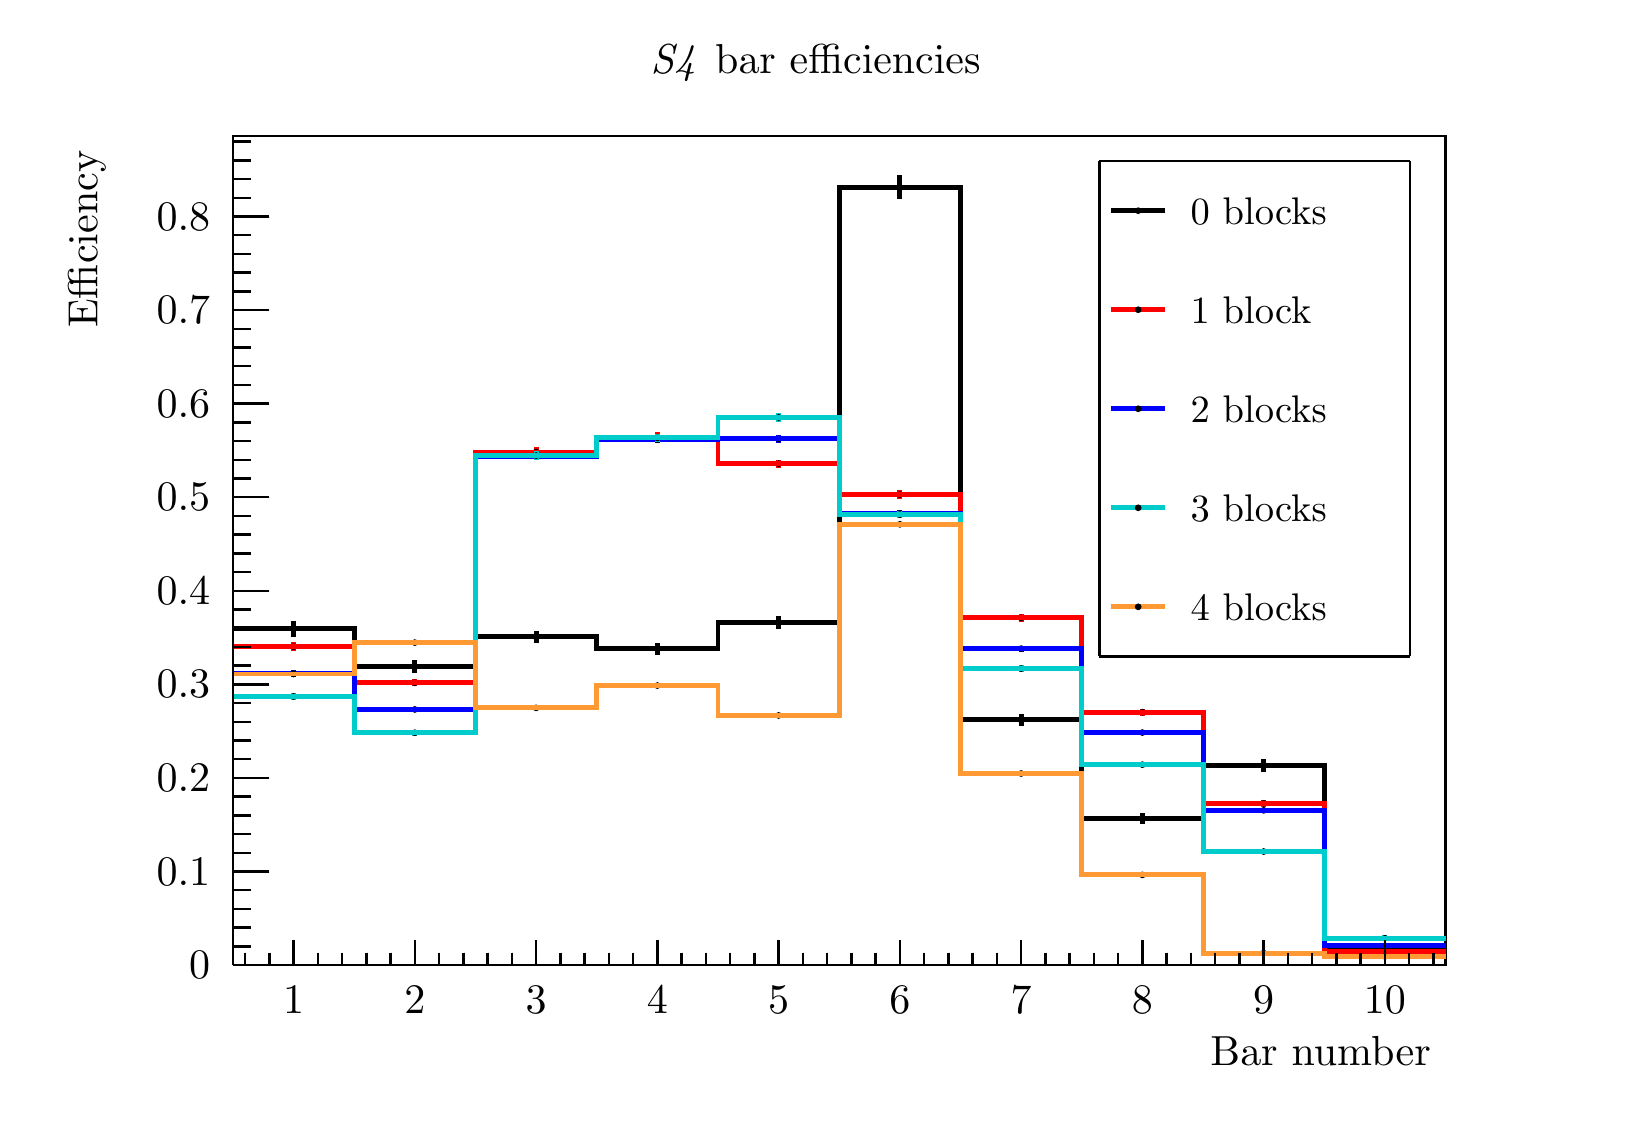
\begin{tikzpicture}
\pgfdeclareplotmark{cross} {
\pgfpathmoveto{\pgfpoint{-0.3\pgfplotmarksize}{\pgfplotmarksize}}
\pgfpathlineto{\pgfpoint{+0.3\pgfplotmarksize}{\pgfplotmarksize}}
\pgfpathlineto{\pgfpoint{+0.3\pgfplotmarksize}{0.3\pgfplotmarksize}}
\pgfpathlineto{\pgfpoint{+1\pgfplotmarksize}{0.3\pgfplotmarksize}}
\pgfpathlineto{\pgfpoint{+1\pgfplotmarksize}{-0.3\pgfplotmarksize}}
\pgfpathlineto{\pgfpoint{+0.3\pgfplotmarksize}{-0.3\pgfplotmarksize}}
\pgfpathlineto{\pgfpoint{+0.3\pgfplotmarksize}{-1.\pgfplotmarksize}}
\pgfpathlineto{\pgfpoint{-0.3\pgfplotmarksize}{-1.\pgfplotmarksize}}
\pgfpathlineto{\pgfpoint{-0.3\pgfplotmarksize}{-0.3\pgfplotmarksize}}
\pgfpathlineto{\pgfpoint{-1.\pgfplotmarksize}{-0.3\pgfplotmarksize}}
\pgfpathlineto{\pgfpoint{-1.\pgfplotmarksize}{0.3\pgfplotmarksize}}
\pgfpathlineto{\pgfpoint{-0.3\pgfplotmarksize}{0.3\pgfplotmarksize}}
\pgfpathclose
\pgfusepathqstroke
}
\pgfdeclareplotmark{cross*} {
\pgfpathmoveto{\pgfpoint{-0.3\pgfplotmarksize}{\pgfplotmarksize}}
\pgfpathlineto{\pgfpoint{+0.3\pgfplotmarksize}{\pgfplotmarksize}}
\pgfpathlineto{\pgfpoint{+0.3\pgfplotmarksize}{0.3\pgfplotmarksize}}
\pgfpathlineto{\pgfpoint{+1\pgfplotmarksize}{0.3\pgfplotmarksize}}
\pgfpathlineto{\pgfpoint{+1\pgfplotmarksize}{-0.3\pgfplotmarksize}}
\pgfpathlineto{\pgfpoint{+0.3\pgfplotmarksize}{-0.3\pgfplotmarksize}}
\pgfpathlineto{\pgfpoint{+0.3\pgfplotmarksize}{-1.\pgfplotmarksize}}
\pgfpathlineto{\pgfpoint{-0.3\pgfplotmarksize}{-1.\pgfplotmarksize}}
\pgfpathlineto{\pgfpoint{-0.3\pgfplotmarksize}{-0.3\pgfplotmarksize}}
\pgfpathlineto{\pgfpoint{-1.\pgfplotmarksize}{-0.3\pgfplotmarksize}}
\pgfpathlineto{\pgfpoint{-1.\pgfplotmarksize}{0.3\pgfplotmarksize}}
\pgfpathlineto{\pgfpoint{-0.3\pgfplotmarksize}{0.3\pgfplotmarksize}}
\pgfpathclose
\pgfusepathqfillstroke
}
\pgfdeclareplotmark{newstar} {
\pgfpathmoveto{\pgfqpoint{0pt}{\pgfplotmarksize}}
\pgfpathlineto{\pgfqpointpolar{44}{0.5\pgfplotmarksize}}
\pgfpathlineto{\pgfqpointpolar{18}{\pgfplotmarksize}}
\pgfpathlineto{\pgfqpointpolar{-20}{0.5\pgfplotmarksize}}
\pgfpathlineto{\pgfqpointpolar{-54}{\pgfplotmarksize}}
\pgfpathlineto{\pgfqpointpolar{-90}{0.5\pgfplotmarksize}}
\pgfpathlineto{\pgfqpointpolar{234}{\pgfplotmarksize}}
\pgfpathlineto{\pgfqpointpolar{198}{0.5\pgfplotmarksize}}
\pgfpathlineto{\pgfqpointpolar{162}{\pgfplotmarksize}}
\pgfpathlineto{\pgfqpointpolar{134}{0.5\pgfplotmarksize}}
\pgfpathclose
\pgfusepathqstroke
}
\pgfdeclareplotmark{newstar*} {
\pgfpathmoveto{\pgfqpoint{0pt}{\pgfplotmarksize}}
\pgfpathlineto{\pgfqpointpolar{44}{0.5\pgfplotmarksize}}
\pgfpathlineto{\pgfqpointpolar{18}{\pgfplotmarksize}}
\pgfpathlineto{\pgfqpointpolar{-20}{0.5\pgfplotmarksize}}
\pgfpathlineto{\pgfqpointpolar{-54}{\pgfplotmarksize}}
\pgfpathlineto{\pgfqpointpolar{-90}{0.5\pgfplotmarksize}}
\pgfpathlineto{\pgfqpointpolar{234}{\pgfplotmarksize}}
\pgfpathlineto{\pgfqpointpolar{198}{0.5\pgfplotmarksize}}
\pgfpathlineto{\pgfqpointpolar{162}{\pgfplotmarksize}}
\pgfpathlineto{\pgfqpointpolar{134}{0.5\pgfplotmarksize}}
\pgfpathclose
\pgfusepathqfillstroke
}
\definecolor{c}{rgb}{1,1,1};
\draw [color=c, fill=c] (0,0) rectangle (20,13.6752);
\draw [color=c, fill=c] (2.6,1.77778) rectangle (18,12.3077);
\definecolor{c}{rgb}{0,0,0};
\draw [c,line width=0.9] (2.6,1.77778) -- (2.6,12.3077) -- (18,12.3077) -- (18,1.77778) -- (2.6,1.77778);
\definecolor{c}{rgb}{1,1,1};
\draw [color=c, fill=c] (2.6,1.77778) rectangle (18,12.3077);
\definecolor{c}{rgb}{0,0,0};
\draw [c,line width=0.9] (2.6,1.77778) -- (2.6,12.3077) -- (18,12.3077) -- (18,1.77778) -- (2.6,1.77778);
\definecolor{c}{rgb}{0,0,0.6};
\draw [c,line width=0.9] (2.6,1.77778) -- (4.14,1.77778) -- (4.14,1.77778) -- (5.68,1.77778) -- (5.68,1.77778) -- (7.22,1.77778) -- (7.22,1.77778) -- (8.76,1.77778) -- (8.76,1.77778) -- (10.3,1.77778) -- (10.3,1.77778) -- (11.84,1.77778) --
 (11.84,1.77778) -- (13.38,1.77778) -- (13.38,1.77778) -- (14.92,1.77778) -- (14.92,1.77778) -- (16.46,1.77778) -- (16.46,1.77778) -- (18,1.77778);
\definecolor{c}{rgb}{0,0,0};
\draw [c,line width=0.9] (2.6,1.77778) -- (18,1.77778);
\draw [c,line width=0.9] (3.37,2.09368) -- (3.37,1.77778);
\draw [c,line width=0.9] (3.678,1.93573) -- (3.678,1.77778);
\draw [c,line width=0.9] (3.986,1.93573) -- (3.986,1.77778);
\draw [c,line width=0.9] (4.294,1.93573) -- (4.294,1.77778);
\draw [c,line width=0.9] (4.602,1.93573) -- (4.602,1.77778);
\draw [c,line width=0.9] (4.91,2.09368) -- (4.91,1.77778);
\draw [c,line width=0.9] (5.218,1.93573) -- (5.218,1.77778);
\draw [c,line width=0.9] (5.526,1.93573) -- (5.526,1.77778);
\draw [c,line width=0.9] (5.834,1.93573) -- (5.834,1.77778);
\draw [c,line width=0.9] (6.142,1.93573) -- (6.142,1.77778);
\draw [c,line width=0.9] (6.45,2.09368) -- (6.45,1.77778);
\draw [c,line width=0.9] (6.758,1.93573) -- (6.758,1.77778);
\draw [c,line width=0.9] (7.066,1.93573) -- (7.066,1.77778);
\draw [c,line width=0.9] (7.374,1.93573) -- (7.374,1.77778);
\draw [c,line width=0.9] (7.682,1.93573) -- (7.682,1.77778);
\draw [c,line width=0.9] (7.99,2.09368) -- (7.99,1.77778);
\draw [c,line width=0.9] (8.298,1.93573) -- (8.298,1.77778);
\draw [c,line width=0.9] (8.606,1.93573) -- (8.606,1.77778);
\draw [c,line width=0.9] (8.914,1.93573) -- (8.914,1.77778);
\draw [c,line width=0.9] (9.222,1.93573) -- (9.222,1.77778);
\draw [c,line width=0.9] (9.53,2.09368) -- (9.53,1.77778);
\draw [c,line width=0.9] (9.838,1.93573) -- (9.838,1.77778);
\draw [c,line width=0.9] (10.146,1.93573) -- (10.146,1.77778);
\draw [c,line width=0.9] (10.454,1.93573) -- (10.454,1.77778);
\draw [c,line width=0.9] (10.762,1.93573) -- (10.762,1.77778);
\draw [c,line width=0.9] (11.07,2.09368) -- (11.07,1.77778);
\draw [c,line width=0.9] (11.378,1.93573) -- (11.378,1.77778);
\draw [c,line width=0.9] (11.686,1.93573) -- (11.686,1.77778);
\draw [c,line width=0.9] (11.994,1.93573) -- (11.994,1.77778);
\draw [c,line width=0.9] (12.302,1.93573) -- (12.302,1.77778);
\draw [c,line width=0.9] (12.61,2.09368) -- (12.61,1.77778);
\draw [c,line width=0.9] (12.918,1.93573) -- (12.918,1.77778);
\draw [c,line width=0.9] (13.226,1.93573) -- (13.226,1.77778);
\draw [c,line width=0.9] (13.534,1.93573) -- (13.534,1.77778);
\draw [c,line width=0.9] (13.842,1.93573) -- (13.842,1.77778);
\draw [c,line width=0.9] (14.15,2.09368) -- (14.15,1.77778);
\draw [c,line width=0.9] (14.458,1.93573) -- (14.458,1.77778);
\draw [c,line width=0.9] (14.766,1.93573) -- (14.766,1.77778);
\draw [c,line width=0.9] (15.074,1.93573) -- (15.074,1.77778);
\draw [c,line width=0.9] (15.382,1.93573) -- (15.382,1.77778);
\draw [c,line width=0.9] (15.69,2.09368) -- (15.69,1.77778);
\draw [c,line width=0.9] (15.998,1.93573) -- (15.998,1.77778);
\draw [c,line width=0.9] (16.306,1.93573) -- (16.306,1.77778);
\draw [c,line width=0.9] (16.614,1.93573) -- (16.614,1.77778);
\draw [c,line width=0.9] (16.922,1.93573) -- (16.922,1.77778);
\draw [c,line width=0.9] (17.23,2.09368) -- (17.23,1.77778);
\draw [c,line width=0.9] (3.37,2.09368) -- (3.37,1.77778);
\draw [c,line width=0.9] (3.062,1.93573) -- (3.062,1.77778);
\draw [c,line width=0.9] (2.754,1.93573) -- (2.754,1.77778);
\draw [c,line width=0.9] (17.23,2.09368) -- (17.23,1.77778);
\draw [c,line width=0.9] (17.538,1.93573) -- (17.538,1.77778);
\draw [c,line width=0.9] (17.846,1.93573) -- (17.846,1.77778);
\draw [anchor=base] (3.37,1.16239) node[scale=1.51861, color=c, rotate=0]{1};
\draw [anchor=base] (4.91,1.16239) node[scale=1.51861, color=c, rotate=0]{2};
\draw [anchor=base] (6.45,1.16239) node[scale=1.51861, color=c, rotate=0]{3};
\draw [anchor=base] (7.99,1.16239) node[scale=1.51861, color=c, rotate=0]{4};
\draw [anchor=base] (9.53,1.16239) node[scale=1.51861, color=c, rotate=0]{5};
\draw [anchor=base] (11.07,1.16239) node[scale=1.51861, color=c, rotate=0]{6};
\draw [anchor=base] (12.61,1.16239) node[scale=1.51861, color=c, rotate=0]{7};
\draw [anchor=base] (14.15,1.16239) node[scale=1.51861, color=c, rotate=0]{8};
\draw [anchor=base] (15.69,1.16239) node[scale=1.51861, color=c, rotate=0]{9};
\draw [anchor=base] (17.23,1.16239) node[scale=1.51861, color=c, rotate=0]{10};
\draw [anchor= east] (18,0.683761) node[scale=1.51861, color=c, rotate=0]{ Bar number};
\draw [c,line width=0.9] (2.6,1.77778) -- (2.6,12.3077);
\draw [c,line width=0.9] (3.062,1.77778) -- (2.6,1.77778);
\draw [c,line width=0.9] (2.831,2.01544) -- (2.6,2.01544);
\draw [c,line width=0.9] (2.831,2.2531) -- (2.6,2.2531);
\draw [c,line width=0.9] (2.831,2.49075) -- (2.6,2.49075);
\draw [c,line width=0.9] (2.831,2.72841) -- (2.6,2.72841);
\draw [c,line width=0.9] (3.062,2.96607) -- (2.6,2.96607);
\draw [c,line width=0.9] (2.831,3.20373) -- (2.6,3.20373);
\draw [c,line width=0.9] (2.831,3.44139) -- (2.6,3.44139);
\draw [c,line width=0.9] (2.831,3.67905) -- (2.6,3.67905);
\draw [c,line width=0.9] (2.831,3.91671) -- (2.6,3.91671);
\draw [c,line width=0.9] (3.062,4.15437) -- (2.6,4.15437);
\draw [c,line width=0.9] (2.831,4.39202) -- (2.6,4.39202);
\draw [c,line width=0.9] (2.831,4.62968) -- (2.6,4.62968);
\draw [c,line width=0.9] (2.831,4.86734) -- (2.6,4.86734);
\draw [c,line width=0.9] (2.831,5.105) -- (2.6,5.105);
\draw [c,line width=0.9] (3.062,5.34266) -- (2.6,5.34266);
\draw [c,line width=0.9] (2.831,5.58032) -- (2.6,5.58032);
\draw [c,line width=0.9] (2.831,5.81798) -- (2.6,5.81798);
\draw [c,line width=0.9] (2.831,6.05563) -- (2.6,6.05563);
\draw [c,line width=0.9] (2.831,6.29329) -- (2.6,6.29329);
\draw [c,line width=0.9] (3.062,6.53095) -- (2.6,6.53095);
\draw [c,line width=0.9] (2.831,6.76861) -- (2.6,6.76861);
\draw [c,line width=0.9] (2.831,7.00627) -- (2.6,7.00627);
\draw [c,line width=0.9] (2.831,7.24393) -- (2.6,7.24393);
\draw [c,line width=0.9] (2.831,7.48159) -- (2.6,7.48159);
\draw [c,line width=0.9] (3.062,7.71925) -- (2.6,7.71925);
\draw [c,line width=0.9] (2.831,7.9569) -- (2.6,7.9569);
\draw [c,line width=0.9] (2.831,8.19456) -- (2.6,8.19456);
\draw [c,line width=0.9] (2.831,8.43222) -- (2.6,8.43222);
\draw [c,line width=0.9] (2.831,8.66988) -- (2.6,8.66988);
\draw [c,line width=0.9] (3.062,8.90754) -- (2.6,8.90754);
\draw [c,line width=0.9] (2.831,9.1452) -- (2.6,9.1452);
\draw [c,line width=0.9] (2.831,9.38286) -- (2.6,9.38286);
\draw [c,line width=0.9] (2.831,9.62052) -- (2.6,9.62052);
\draw [c,line width=0.9] (2.831,9.85817) -- (2.6,9.85817);
\draw [c,line width=0.9] (3.062,10.0958) -- (2.6,10.0958);
\draw [c,line width=0.9] (2.831,10.3335) -- (2.6,10.3335);
\draw [c,line width=0.9] (2.831,10.5711) -- (2.6,10.5711);
\draw [c,line width=0.9] (2.831,10.8088) -- (2.6,10.8088);
\draw [c,line width=0.9] (2.831,11.0465) -- (2.6,11.0465);
\draw [c,line width=0.9] (3.062,11.2841) -- (2.6,11.2841);
\draw [c,line width=0.9] (3.062,11.2841) -- (2.6,11.2841);
\draw [c,line width=0.9] (2.831,11.5218) -- (2.6,11.5218);
\draw [c,line width=0.9] (2.831,11.7594) -- (2.6,11.7594);
\draw [c,line width=0.9] (2.831,11.9971) -- (2.6,11.9971);
\draw [c,line width=0.9] (2.831,12.2348) -- (2.6,12.2348);
\draw [anchor= east] (2.5,1.77778) node[scale=1.51861, color=c, rotate=0]{0};
\draw [anchor= east] (2.5,2.96607) node[scale=1.51861, color=c, rotate=0]{0.1};
\draw [anchor= east] (2.5,4.15437) node[scale=1.51861, color=c, rotate=0]{0.2};
\draw [anchor= east] (2.5,5.34266) node[scale=1.51861, color=c, rotate=0]{0.3};
\draw [anchor= east] (2.5,6.53095) node[scale=1.51861, color=c, rotate=0]{0.4};
\draw [anchor= east] (2.5,7.71925) node[scale=1.51861, color=c, rotate=0]{0.5};
\draw [anchor= east] (2.5,8.90754) node[scale=1.51861, color=c, rotate=0]{0.6};
\draw [anchor= east] (2.5,10.0958) node[scale=1.51861, color=c, rotate=0]{0.7};
\draw [anchor= east] (2.5,11.2841) node[scale=1.51861, color=c, rotate=0]{0.8};
\draw [anchor= east] (0.745299,12.3077) node[scale=1.51861, color=c, rotate=90]{ Efficiency};
\draw [c,line width=1.8] (3.37,5.94713) -- (3.37,6.048);
\draw [c,line width=1.8] (3.37,6.048) -- (3.37,6.14887);
\foreach \P in {(3.37,6.048)}{\draw[mark options={color=c,fill=c},mark size=2.402402pt,mark=*,mark size=1pt] plot coordinates {\P};}
\draw [c,line width=1.8] (4.91,5.48652) -- (4.91,5.56707);
\draw [c,line width=1.8] (4.91,5.56707) -- (4.91,5.64763);
\foreach \P in {(4.91,5.56707)}{\draw[mark options={color=c,fill=c},mark size=2.402402pt,mark=*,mark size=1pt] plot coordinates {\P};}
\draw [c,line width=1.8] (6.45,5.86443) -- (6.45,5.94509);
\draw [c,line width=1.8] (6.45,5.94509) -- (6.45,6.02574);
\foreach \P in {(6.45,5.94509)}{\draw[mark options={color=c,fill=c},mark size=2.402402pt,mark=*,mark size=1pt] plot coordinates {\P};}
\draw [c,line width=1.8] (7.99,5.72099) -- (7.99,5.79421);
\draw [c,line width=1.8] (7.99,5.79421) -- (7.99,5.86742);
\foreach \P in {(7.99,5.79421)}{\draw[mark options={color=c,fill=c},mark size=2.402402pt,mark=*,mark size=1pt] plot coordinates {\P};}
\draw [c,line width=1.8] (9.53,6.04947) -- (9.53,6.12746);
\draw [c,line width=1.8] (9.53,6.12746) -- (9.53,6.20546);
\foreach \P in {(9.53,6.12746)}{\draw[mark options={color=c,fill=c},mark size=2.402402pt,mark=*,mark size=1pt] plot coordinates {\P};}
\draw [c,line width=1.8] (11.07,11.5047) -- (11.07,11.6555);
\draw [c,line width=1.8] (11.07,11.6555) -- (11.07,11.8063);
\foreach \P in {(11.07,11.6555)}{\draw[mark options={color=c,fill=c},mark size=2.402402pt,mark=*,mark size=1pt] plot coordinates {\P};}
\draw [c,line width=1.8] (12.61,4.81396) -- (12.61,4.88993);
\draw [c,line width=1.8] (12.61,4.88993) -- (12.61,4.96589);
\foreach \P in {(12.61,4.88993)}{\draw[mark options={color=c,fill=c},mark size=2.402402pt,mark=*,mark size=1pt] plot coordinates {\P};}
\draw [c,line width=1.8] (14.15,3.56561) -- (14.15,3.63618);
\draw [c,line width=1.8] (14.15,3.63618) -- (14.15,3.70674);
\foreach \P in {(14.15,3.63618)}{\draw[mark options={color=c,fill=c},mark size=2.402402pt,mark=*,mark size=1pt] plot coordinates {\P};}
\draw [c,line width=1.8] (15.69,4.23443) -- (15.69,4.31531);
\draw [c,line width=1.8] (15.69,4.31531) -- (15.69,4.39619);
\foreach \P in {(15.69,4.31531)}{\draw[mark options={color=c,fill=c},mark size=2.402402pt,mark=*,mark size=1pt] plot coordinates {\P};}
\draw [c,line width=1.8] (17.23,1.95841) -- (17.23,2.00004);
\draw [c,line width=1.8] (17.23,2.00004) -- (17.23,2.04166);
\foreach \P in {(17.23,2.00004)}{\draw[mark options={color=c,fill=c},mark size=2.402402pt,mark=*,mark size=1pt] plot coordinates {\P};}
\draw [c,line width=1.8] (2.6,6.048) -- (4.14,6.048) -- (4.14,5.56707) -- (5.68,5.56707) -- (5.68,5.94509) -- (7.22,5.94509) -- (7.22,5.79421) -- (8.76,5.79421) -- (8.76,6.12746) -- (10.3,6.12746) -- (10.3,11.6555) -- (11.84,11.6555) --
 (11.84,4.88993) -- (13.38,4.88993) -- (13.38,3.63618) -- (14.92,3.63618) -- (14.92,4.31531) -- (16.46,4.31531) -- (16.46,2.00004) -- (18,2.00004);
\definecolor{c}{rgb}{1,0,0};
\draw [c,line width=1.8] (3.37,5.76471) -- (3.37,5.8214);
\draw [c,line width=1.8] (3.37,5.8214) -- (3.37,5.8781);
\definecolor{c}{rgb}{0,0,0};
\foreach \P in {(3.37,5.8214)}{\draw[mark options={color=c,fill=c},mark size=2.402402pt,mark=*,mark size=1pt] plot coordinates {\P};}
\definecolor{c}{rgb}{1,0,0};
\draw [c,line width=1.8] (4.91,5.31634) -- (4.91,5.36213);
\draw [c,line width=1.8] (4.91,5.36213) -- (4.91,5.40793);
\definecolor{c}{rgb}{0,0,0};
\foreach \P in {(4.91,5.36213)}{\draw[mark options={color=c,fill=c},mark size=2.402402pt,mark=*,mark size=1pt] plot coordinates {\P};}
\definecolor{c}{rgb}{1,0,0};
\draw [c,line width=1.8] (6.45,8.23172) -- (6.45,8.29272);
\draw [c,line width=1.8] (6.45,8.29272) -- (6.45,8.35373);
\definecolor{c}{rgb}{0,0,0};
\foreach \P in {(6.45,8.29272)}{\draw[mark options={color=c,fill=c},mark size=2.402402pt,mark=*,mark size=1pt] plot coordinates {\P};}
\definecolor{c}{rgb}{1,0,0};
\draw [c,line width=1.8] (7.99,8.42349) -- (7.99,8.48284);
\draw [c,line width=1.8] (7.99,8.48284) -- (7.99,8.5422);
\definecolor{c}{rgb}{0,0,0};
\foreach \P in {(7.99,8.48284)}{\draw[mark options={color=c,fill=c},mark size=2.402402pt,mark=*,mark size=1pt] plot coordinates {\P};}
\definecolor{c}{rgb}{1,0,0};
\draw [c,line width=1.8] (9.53,8.09169) -- (9.53,8.14475);
\draw [c,line width=1.8] (9.53,8.14475) -- (9.53,8.1978);
\definecolor{c}{rgb}{0,0,0};
\foreach \P in {(9.53,8.14475)}{\draw[mark options={color=c,fill=c},mark size=2.402402pt,mark=*,mark size=1pt] plot coordinates {\P};}
\definecolor{c}{rgb}{1,0,0};
\draw [c,line width=1.8] (11.07,7.69589) -- (11.07,7.75308);
\draw [c,line width=1.8] (11.07,7.75308) -- (11.07,7.81026);
\definecolor{c}{rgb}{0,0,0};
\foreach \P in {(11.07,7.75308)}{\draw[mark options={color=c,fill=c},mark size=2.402402pt,mark=*,mark size=1pt] plot coordinates {\P};}
\definecolor{c}{rgb}{1,0,0};
\draw [c,line width=1.8] (12.61,6.13603) -- (12.61,6.1871);
\draw [c,line width=1.8] (12.61,6.1871) -- (12.61,6.23818);
\definecolor{c}{rgb}{0,0,0};
\foreach \P in {(12.61,6.1871)}{\draw[mark options={color=c,fill=c},mark size=2.402402pt,mark=*,mark size=1pt] plot coordinates {\P};}
\definecolor{c}{rgb}{1,0,0};
\draw [c,line width=1.8] (14.15,4.9422) -- (14.15,4.9889);
\draw [c,line width=1.8] (14.15,4.9889) -- (14.15,5.0356);
\definecolor{c}{rgb}{0,0,0};
\foreach \P in {(14.15,4.9889)}{\draw[mark options={color=c,fill=c},mark size=2.402402pt,mark=*,mark size=1pt] plot coordinates {\P};}
\definecolor{c}{rgb}{1,0,0};
\draw [c,line width=1.8] (15.69,3.78842) -- (15.69,3.83138);
\draw [c,line width=1.8] (15.69,3.83138) -- (15.69,3.87434);
\definecolor{c}{rgb}{0,0,0};
\foreach \P in {(15.69,3.83138)}{\draw[mark options={color=c,fill=c},mark size=2.402402pt,mark=*,mark size=1pt] plot coordinates {\P};}
\definecolor{c}{rgb}{1,0,0};
\draw [c,line width=1.8] (17.23,1.91836) -- (17.23,1.9483);
\draw [c,line width=1.8] (17.23,1.9483) -- (17.23,1.97823);
\definecolor{c}{rgb}{0,0,0};
\foreach \P in {(17.23,1.9483)}{\draw[mark options={color=c,fill=c},mark size=2.402402pt,mark=*,mark size=1pt] plot coordinates {\P};}
\definecolor{c}{rgb}{1,0,0};
\draw [c,line width=1.8] (2.6,5.8214) -- (4.14,5.8214) -- (4.14,5.36213) -- (5.68,5.36213) -- (5.68,8.29272) -- (7.22,8.29272) -- (7.22,8.48284) -- (8.76,8.48284) -- (8.76,8.14475) -- (10.3,8.14475) -- (10.3,7.75308) -- (11.84,7.75308) --
 (11.84,6.1871) -- (13.38,6.1871) -- (13.38,4.9889) -- (14.92,4.9889) -- (14.92,3.83138) -- (16.46,3.83138) -- (16.46,1.9483) -- (18,1.9483);
\definecolor{c}{rgb}{0,0,1};
\draw [c,line width=1.8] (3.37,5.43835) -- (3.37,5.48052);
\draw [c,line width=1.8] (3.37,5.48052) -- (3.37,5.52268);
\definecolor{c}{rgb}{0,0,0};
\foreach \P in {(3.37,5.48052)}{\draw[mark options={color=c,fill=c},mark size=2.402402pt,mark=*,mark size=1pt] plot coordinates {\P};}
\definecolor{c}{rgb}{0,0,1};
\draw [c,line width=1.8] (4.91,4.9892) -- (4.91,5.02356);
\draw [c,line width=1.8] (4.91,5.02356) -- (4.91,5.05792);
\definecolor{c}{rgb}{0,0,0};
\foreach \P in {(4.91,5.02356)}{\draw[mark options={color=c,fill=c},mark size=2.402402pt,mark=*,mark size=1pt] plot coordinates {\P};}
\definecolor{c}{rgb}{0,0,1};
\draw [c,line width=1.8] (6.45,8.19027) -- (6.45,8.23881);
\draw [c,line width=1.8] (6.45,8.23881) -- (6.45,8.28735);
\definecolor{c}{rgb}{0,0,0};
\foreach \P in {(6.45,8.23881)}{\draw[mark options={color=c,fill=c},mark size=2.402402pt,mark=*,mark size=1pt] plot coordinates {\P};}
\definecolor{c}{rgb}{0,0,1};
\draw [c,line width=1.8] (7.99,8.40121) -- (7.99,8.44901);
\draw [c,line width=1.8] (7.99,8.44901) -- (7.99,8.49681);
\definecolor{c}{rgb}{0,0,0};
\foreach \P in {(7.99,8.44901)}{\draw[mark options={color=c,fill=c},mark size=2.402402pt,mark=*,mark size=1pt] plot coordinates {\P};}
\definecolor{c}{rgb}{0,0,1};
\draw [c,line width=1.8] (9.53,8.41363) -- (9.53,8.45921);
\draw [c,line width=1.8] (9.53,8.45921) -- (9.53,8.50478);
\definecolor{c}{rgb}{0,0,0};
\foreach \P in {(9.53,8.45921)}{\draw[mark options={color=c,fill=c},mark size=2.402402pt,mark=*,mark size=1pt] plot coordinates {\P};}
\definecolor{c}{rgb}{0,0,1};
\draw [c,line width=1.8] (11.07,7.46957) -- (11.07,7.51425);
\draw [c,line width=1.8] (11.07,7.51425) -- (11.07,7.55892);
\definecolor{c}{rgb}{0,0,0};
\foreach \P in {(11.07,7.51425)}{\draw[mark options={color=c,fill=c},mark size=2.402402pt,mark=*,mark size=1pt] plot coordinates {\P};}
\definecolor{c}{rgb}{0,0,1};
\draw [c,line width=1.8] (12.61,5.75818) -- (12.61,5.79638);
\draw [c,line width=1.8] (12.61,5.79638) -- (12.61,5.83458);
\definecolor{c}{rgb}{0,0,0};
\foreach \P in {(12.61,5.79638)}{\draw[mark options={color=c,fill=c},mark size=2.402402pt,mark=*,mark size=1pt] plot coordinates {\P};}
\definecolor{c}{rgb}{0,0,1};
\draw [c,line width=1.8] (14.15,4.69542) -- (14.15,4.73);
\draw [c,line width=1.8] (14.15,4.73) -- (14.15,4.76458);
\definecolor{c}{rgb}{0,0,0};
\foreach \P in {(14.15,4.73)}{\draw[mark options={color=c,fill=c},mark size=2.402402pt,mark=*,mark size=1pt] plot coordinates {\P};}
\definecolor{c}{rgb}{0,0,1};
\draw [c,line width=1.8] (15.69,3.71002) -- (15.69,3.74208);
\draw [c,line width=1.8] (15.69,3.74208) -- (15.69,3.77415);
\definecolor{c}{rgb}{0,0,0};
\foreach \P in {(15.69,3.74208)}{\draw[mark options={color=c,fill=c},mark size=2.402402pt,mark=*,mark size=1pt] plot coordinates {\P};}
\definecolor{c}{rgb}{0,0,1};
\draw [c,line width=1.8] (17.23,1.99459) -- (17.23,2.02279);
\draw [c,line width=1.8] (17.23,2.02279) -- (17.23,2.05099);
\definecolor{c}{rgb}{0,0,0};
\foreach \P in {(17.23,2.02279)}{\draw[mark options={color=c,fill=c},mark size=2.402402pt,mark=*,mark size=1pt] plot coordinates {\P};}
\definecolor{c}{rgb}{0,0,1};
\draw [c,line width=1.8] (2.6,5.48052) -- (4.14,5.48052) -- (4.14,5.02356) -- (5.68,5.02356) -- (5.68,8.23881) -- (7.22,8.23881) -- (7.22,8.44901) -- (8.76,8.44901) -- (8.76,8.45921) -- (10.3,8.45921) -- (10.3,7.51425) -- (11.84,7.51425) --
 (11.84,5.79638) -- (13.38,5.79638) -- (13.38,4.73) -- (14.92,4.73) -- (14.92,3.74208) -- (16.46,3.74208) -- (16.46,2.02279) -- (18,2.02279);
\definecolor{c}{rgb}{0,0.8,0.8};
\draw [c,line width=1.8] (3.37,5.14512) -- (3.37,5.18859);
\draw [c,line width=1.8] (3.37,5.18859) -- (3.37,5.23205);
\definecolor{c}{rgb}{0,0,0};
\foreach \P in {(3.37,5.18859)}{\draw[mark options={color=c,fill=c},mark size=2.402402pt,mark=*,mark size=1pt] plot coordinates {\P};}
\definecolor{c}{rgb}{0,0.8,0.8};
\draw [c,line width=1.8] (4.91,4.69231) -- (4.91,4.72802);
\draw [c,line width=1.8] (4.91,4.72802) -- (4.91,4.76372);
\definecolor{c}{rgb}{0,0,0};
\foreach \P in {(4.91,4.72802)}{\draw[mark options={color=c,fill=c},mark size=2.402402pt,mark=*,mark size=1pt] plot coordinates {\P};}
\definecolor{c}{rgb}{0,0.8,0.8};
\draw [c,line width=1.8] (6.45,8.19462) -- (6.45,8.2476);
\draw [c,line width=1.8] (6.45,8.2476) -- (6.45,8.30059);
\definecolor{c}{rgb}{0,0,0};
\foreach \P in {(6.45,8.2476)}{\draw[mark options={color=c,fill=c},mark size=2.402402pt,mark=*,mark size=1pt] plot coordinates {\P};}
\definecolor{c}{rgb}{0,0.8,0.8};
\draw [c,line width=1.8] (7.99,8.41839) -- (7.99,8.47122);
\draw [c,line width=1.8] (7.99,8.47122) -- (7.99,8.52405);
\definecolor{c}{rgb}{0,0,0};
\foreach \P in {(7.99,8.47122)}{\draw[mark options={color=c,fill=c},mark size=2.402402pt,mark=*,mark size=1pt] plot coordinates {\P};}
\definecolor{c}{rgb}{0,0.8,0.8};
\draw [c,line width=1.8] (9.53,8.67919) -- (9.53,8.73184);
\draw [c,line width=1.8] (9.53,8.73184) -- (9.53,8.78449);
\definecolor{c}{rgb}{0,0,0};
\foreach \P in {(9.53,8.73184)}{\draw[mark options={color=c,fill=c},mark size=2.402402pt,mark=*,mark size=1pt] plot coordinates {\P};}
\definecolor{c}{rgb}{0,0.8,0.8};
\draw [c,line width=1.8] (11.07,7.44878) -- (11.07,7.49768);
\draw [c,line width=1.8] (11.07,7.49768) -- (11.07,7.54658);
\definecolor{c}{rgb}{0,0,0};
\foreach \P in {(11.07,7.49768)}{\draw[mark options={color=c,fill=c},mark size=2.402402pt,mark=*,mark size=1pt] plot coordinates {\P};}
\definecolor{c}{rgb}{0,0.8,0.8};
\draw [c,line width=1.8] (12.61,5.50194) -- (12.61,5.54215);
\draw [c,line width=1.8] (12.61,5.54215) -- (12.61,5.58236);
\definecolor{c}{rgb}{0,0,0};
\foreach \P in {(12.61,5.54215)}{\draw[mark options={color=c,fill=c},mark size=2.402402pt,mark=*,mark size=1pt] plot coordinates {\P};}
\definecolor{c}{rgb}{0,0.8,0.8};
\draw [c,line width=1.8] (14.15,4.28775) -- (14.15,4.32232);
\draw [c,line width=1.8] (14.15,4.32232) -- (14.15,4.3569);
\definecolor{c}{rgb}{0,0,0};
\foreach \P in {(14.15,4.32232)}{\draw[mark options={color=c,fill=c},mark size=2.402402pt,mark=*,mark size=1pt] plot coordinates {\P};}
\definecolor{c}{rgb}{0,0.8,0.8};
\draw [c,line width=1.8] (15.69,3.18971) -- (15.69,3.21924);
\draw [c,line width=1.8] (15.69,3.21924) -- (15.69,3.24878);
\definecolor{c}{rgb}{0,0,0};
\foreach \P in {(15.69,3.21924)}{\draw[mark options={color=c,fill=c},mark size=2.402402pt,mark=*,mark size=1pt] plot coordinates {\P};}
\definecolor{c}{rgb}{0,0.8,0.8};
\draw [c,line width=1.8] (17.23,2.07797) -- (17.23,2.11716);
\draw [c,line width=1.8] (17.23,2.11716) -- (17.23,2.15634);
\definecolor{c}{rgb}{0,0,0};
\foreach \P in {(17.23,2.11716)}{\draw[mark options={color=c,fill=c},mark size=2.402402pt,mark=*,mark size=1pt] plot coordinates {\P};}
\definecolor{c}{rgb}{0,0.8,0.8};
\draw [c,line width=1.8] (2.6,5.18859) -- (4.14,5.18859) -- (4.14,4.72802) -- (5.68,4.72802) -- (5.68,8.2476) -- (7.22,8.2476) -- (7.22,8.47122) -- (8.76,8.47122) -- (8.76,8.73184) -- (10.3,8.73184) -- (10.3,7.49768) -- (11.84,7.49768) --
 (11.84,5.54215) -- (13.38,5.54215) -- (13.38,4.32232) -- (14.92,4.32232) -- (14.92,3.21924) -- (16.46,3.21924) -- (16.46,2.11716) -- (18,2.11716);
\definecolor{c}{rgb}{1,0.6,0.2};
\draw [c,line width=1.8] (3.37,5.46131) -- (3.37,5.47379);
\draw [c,line width=1.8] (3.37,5.47379) -- (3.37,5.48626);
\definecolor{c}{rgb}{0,0,0};
\foreach \P in {(3.37,5.47379)}{\draw[mark options={color=c,fill=c},mark size=2.402402pt,mark=*,mark size=1pt] plot coordinates {\P};}
\definecolor{c}{rgb}{1,0.6,0.2};
\draw [c,line width=1.8] (4.91,5.86106) -- (4.91,5.8726);
\draw [c,line width=1.8] (4.91,5.8726) -- (4.91,5.88414);
\definecolor{c}{rgb}{0,0,0};
\foreach \P in {(4.91,5.8726)}{\draw[mark options={color=c,fill=c},mark size=2.402402pt,mark=*,mark size=1pt] plot coordinates {\P};}
\definecolor{c}{rgb}{1,0.6,0.2};
\draw [c,line width=1.8] (6.45,5.03364) -- (6.45,5.04378);
\draw [c,line width=1.8] (6.45,5.04378) -- (6.45,5.05392);
\definecolor{c}{rgb}{0,0,0};
\foreach \P in {(6.45,5.04378)}{\draw[mark options={color=c,fill=c},mark size=2.402402pt,mark=*,mark size=1pt] plot coordinates {\P};}
\definecolor{c}{rgb}{1,0.6,0.2};
\draw [c,line width=1.8] (7.99,5.31713) -- (7.99,5.32715);
\draw [c,line width=1.8] (7.99,5.32715) -- (7.99,5.33717);
\definecolor{c}{rgb}{0,0,0};
\foreach \P in {(7.99,5.32715)}{\draw[mark options={color=c,fill=c},mark size=2.402402pt,mark=*,mark size=1pt] plot coordinates {\P};}
\definecolor{c}{rgb}{1,0.6,0.2};
\draw [c,line width=1.8] (9.53,4.93765) -- (9.53,4.94748);
\draw [c,line width=1.8] (9.53,4.94748) -- (9.53,4.9573);
\definecolor{c}{rgb}{0,0,0};
\foreach \P in {(9.53,4.94748)}{\draw[mark options={color=c,fill=c},mark size=2.402402pt,mark=*,mark size=1pt] plot coordinates {\P};}
\definecolor{c}{rgb}{1,0.6,0.2};
\draw [c,line width=1.8] (11.07,7.36086) -- (11.07,7.37486);
\draw [c,line width=1.8] (11.07,7.37486) -- (11.07,7.38885);
\definecolor{c}{rgb}{0,0,0};
\foreach \P in {(11.07,7.37486)}{\draw[mark options={color=c,fill=c},mark size=2.402402pt,mark=*,mark size=1pt] plot coordinates {\P};}
\definecolor{c}{rgb}{1,0.6,0.2};
\draw [c,line width=1.8] (12.61,4.20077) -- (12.61,4.21019);
\draw [c,line width=1.8] (12.61,4.21019) -- (12.61,4.21961);
\definecolor{c}{rgb}{0,0,0};
\foreach \P in {(12.61,4.21019)}{\draw[mark options={color=c,fill=c},mark size=2.402402pt,mark=*,mark size=1pt] plot coordinates {\P};}
\definecolor{c}{rgb}{1,0.6,0.2};
\draw [c,line width=1.8] (14.15,2.91481) -- (14.15,2.92264);
\draw [c,line width=1.8] (14.15,2.92264) -- (14.15,2.93048);
\definecolor{c}{rgb}{0,0,0};
\foreach \P in {(14.15,2.92264)}{\draw[mark options={color=c,fill=c},mark size=2.402402pt,mark=*,mark size=1pt] plot coordinates {\P};}
\definecolor{c}{rgb}{1,0.6,0.2};
\draw [c,line width=1.8] (15.69,1.92646) -- (15.69,1.92916);
\draw [c,line width=1.8] (15.69,1.92916) -- (15.69,1.93185);
\definecolor{c}{rgb}{0,0,0};
\foreach \P in {(15.69,1.92916)}{\draw[mark options={color=c,fill=c},mark size=2.402402pt,mark=*,mark size=1pt] plot coordinates {\P};}
\definecolor{c}{rgb}{1,0.6,0.2};
\draw [c,line width=1.8] (17.23,1.88299) -- (17.23,1.88783);
\draw [c,line width=1.8] (17.23,1.88783) -- (17.23,1.89268);
\definecolor{c}{rgb}{0,0,0};
\foreach \P in {(17.23,1.88783)}{\draw[mark options={color=c,fill=c},mark size=2.402402pt,mark=*,mark size=1pt] plot coordinates {\P};}
\definecolor{c}{rgb}{1,0.6,0.2};
\draw [c,line width=1.8] (2.6,5.47379) -- (4.14,5.47379) -- (4.14,5.8726) -- (5.68,5.8726) -- (5.68,5.04378) -- (7.22,5.04378) -- (7.22,5.32715) -- (8.76,5.32715) -- (8.76,4.94748) -- (10.3,4.94748) -- (10.3,7.37486) -- (11.84,7.37486) --
 (11.84,4.21019) -- (13.38,4.21019) -- (13.38,2.92264) -- (14.92,2.92264) -- (14.92,1.92916) -- (16.46,1.92916) -- (16.46,1.88783) -- (18,1.88783);
\definecolor{c}{rgb}{0,0,0};
\draw [c,line width=0.9] (2.6,1.77778) -- (18,1.77778);
\draw [c,line width=0.9] (3.37,2.09368) -- (3.37,1.77778);
\draw [c,line width=0.9] (3.678,1.93573) -- (3.678,1.77778);
\draw [c,line width=0.9] (3.986,1.93573) -- (3.986,1.77778);
\draw [c,line width=0.9] (4.294,1.93573) -- (4.294,1.77778);
\draw [c,line width=0.9] (4.602,1.93573) -- (4.602,1.77778);
\draw [c,line width=0.9] (4.91,2.09368) -- (4.91,1.77778);
\draw [c,line width=0.9] (5.218,1.93573) -- (5.218,1.77778);
\draw [c,line width=0.9] (5.526,1.93573) -- (5.526,1.77778);
\draw [c,line width=0.9] (5.834,1.93573) -- (5.834,1.77778);
\draw [c,line width=0.9] (6.142,1.93573) -- (6.142,1.77778);
\draw [c,line width=0.9] (6.45,2.09368) -- (6.45,1.77778);
\draw [c,line width=0.9] (6.758,1.93573) -- (6.758,1.77778);
\draw [c,line width=0.9] (7.066,1.93573) -- (7.066,1.77778);
\draw [c,line width=0.9] (7.374,1.93573) -- (7.374,1.77778);
\draw [c,line width=0.9] (7.682,1.93573) -- (7.682,1.77778);
\draw [c,line width=0.9] (7.99,2.09368) -- (7.99,1.77778);
\draw [c,line width=0.9] (8.298,1.93573) -- (8.298,1.77778);
\draw [c,line width=0.9] (8.606,1.93573) -- (8.606,1.77778);
\draw [c,line width=0.9] (8.914,1.93573) -- (8.914,1.77778);
\draw [c,line width=0.9] (9.222,1.93573) -- (9.222,1.77778);
\draw [c,line width=0.9] (9.53,2.09368) -- (9.53,1.77778);
\draw [c,line width=0.9] (9.838,1.93573) -- (9.838,1.77778);
\draw [c,line width=0.9] (10.146,1.93573) -- (10.146,1.77778);
\draw [c,line width=0.9] (10.454,1.93573) -- (10.454,1.77778);
\draw [c,line width=0.9] (10.762,1.93573) -- (10.762,1.77778);
\draw [c,line width=0.9] (11.07,2.09368) -- (11.07,1.77778);
\draw [c,line width=0.9] (11.378,1.93573) -- (11.378,1.77778);
\draw [c,line width=0.9] (11.686,1.93573) -- (11.686,1.77778);
\draw [c,line width=0.9] (11.994,1.93573) -- (11.994,1.77778);
\draw [c,line width=0.9] (12.302,1.93573) -- (12.302,1.77778);
\draw [c,line width=0.9] (12.61,2.09368) -- (12.61,1.77778);
\draw [c,line width=0.9] (12.918,1.93573) -- (12.918,1.77778);
\draw [c,line width=0.9] (13.226,1.93573) -- (13.226,1.77778);
\draw [c,line width=0.9] (13.534,1.93573) -- (13.534,1.77778);
\draw [c,line width=0.9] (13.842,1.93573) -- (13.842,1.77778);
\draw [c,line width=0.9] (14.15,2.09368) -- (14.15,1.77778);
\draw [c,line width=0.9] (14.458,1.93573) -- (14.458,1.77778);
\draw [c,line width=0.9] (14.766,1.93573) -- (14.766,1.77778);
\draw [c,line width=0.9] (15.074,1.93573) -- (15.074,1.77778);
\draw [c,line width=0.9] (15.382,1.93573) -- (15.382,1.77778);
\draw [c,line width=0.9] (15.69,2.09368) -- (15.69,1.77778);
\draw [c,line width=0.9] (15.998,1.93573) -- (15.998,1.77778);
\draw [c,line width=0.9] (16.306,1.93573) -- (16.306,1.77778);
\draw [c,line width=0.9] (16.614,1.93573) -- (16.614,1.77778);
\draw [c,line width=0.9] (16.922,1.93573) -- (16.922,1.77778);
\draw [c,line width=0.9] (17.23,2.09368) -- (17.23,1.77778);
\draw [c,line width=0.9] (3.37,2.09368) -- (3.37,1.77778);
\draw [c,line width=0.9] (3.062,1.93573) -- (3.062,1.77778);
\draw [c,line width=0.9] (2.754,1.93573) -- (2.754,1.77778);
\draw [c,line width=0.9] (17.23,2.09368) -- (17.23,1.77778);
\draw [c,line width=0.9] (17.538,1.93573) -- (17.538,1.77778);
\draw [c,line width=0.9] (17.846,1.93573) -- (17.846,1.77778);
\draw [c,line width=0.9] (2.6,1.77778) -- (2.6,12.3077);
\draw [c,line width=0.9] (3.062,1.77778) -- (2.6,1.77778);
\draw [c,line width=0.9] (2.831,2.01544) -- (2.6,2.01544);
\draw [c,line width=0.9] (2.831,2.2531) -- (2.6,2.2531);
\draw [c,line width=0.9] (2.831,2.49075) -- (2.6,2.49075);
\draw [c,line width=0.9] (2.831,2.72841) -- (2.6,2.72841);
\draw [c,line width=0.9] (3.062,2.96607) -- (2.6,2.96607);
\draw [c,line width=0.9] (2.831,3.20373) -- (2.6,3.20373);
\draw [c,line width=0.9] (2.831,3.44139) -- (2.6,3.44139);
\draw [c,line width=0.9] (2.831,3.67905) -- (2.6,3.67905);
\draw [c,line width=0.9] (2.831,3.91671) -- (2.6,3.91671);
\draw [c,line width=0.9] (3.062,4.15437) -- (2.6,4.15437);
\draw [c,line width=0.9] (2.831,4.39202) -- (2.6,4.39202);
\draw [c,line width=0.9] (2.831,4.62968) -- (2.6,4.62968);
\draw [c,line width=0.9] (2.831,4.86734) -- (2.6,4.86734);
\draw [c,line width=0.9] (2.831,5.105) -- (2.6,5.105);
\draw [c,line width=0.9] (3.062,5.34266) -- (2.6,5.34266);
\draw [c,line width=0.9] (2.831,5.58032) -- (2.6,5.58032);
\draw [c,line width=0.9] (2.831,5.81798) -- (2.6,5.81798);
\draw [c,line width=0.9] (2.831,6.05563) -- (2.6,6.05563);
\draw [c,line width=0.9] (2.831,6.29329) -- (2.6,6.29329);
\draw [c,line width=0.9] (3.062,6.53095) -- (2.6,6.53095);
\draw [c,line width=0.9] (2.831,6.76861) -- (2.6,6.76861);
\draw [c,line width=0.9] (2.831,7.00627) -- (2.6,7.00627);
\draw [c,line width=0.9] (2.831,7.24393) -- (2.6,7.24393);
\draw [c,line width=0.9] (2.831,7.48159) -- (2.6,7.48159);
\draw [c,line width=0.9] (3.062,7.71925) -- (2.6,7.71925);
\draw [c,line width=0.9] (2.831,7.9569) -- (2.6,7.9569);
\draw [c,line width=0.9] (2.831,8.19456) -- (2.6,8.19456);
\draw [c,line width=0.9] (2.831,8.43222) -- (2.6,8.43222);
\draw [c,line width=0.9] (2.831,8.66988) -- (2.6,8.66988);
\draw [c,line width=0.9] (3.062,8.90754) -- (2.6,8.90754);
\draw [c,line width=0.9] (2.831,9.1452) -- (2.6,9.1452);
\draw [c,line width=0.9] (2.831,9.38286) -- (2.6,9.38286);
\draw [c,line width=0.9] (2.831,9.62052) -- (2.6,9.62052);
\draw [c,line width=0.9] (2.831,9.85817) -- (2.6,9.85817);
\draw [c,line width=0.9] (3.062,10.0958) -- (2.6,10.0958);
\draw [c,line width=0.9] (2.831,10.3335) -- (2.6,10.3335);
\draw [c,line width=0.9] (2.831,10.5711) -- (2.6,10.5711);
\draw [c,line width=0.9] (2.831,10.8088) -- (2.6,10.8088);
\draw [c,line width=0.9] (2.831,11.0465) -- (2.6,11.0465);
\draw [c,line width=0.9] (3.062,11.2841) -- (2.6,11.2841);
\draw [c,line width=0.9] (3.062,11.2841) -- (2.6,11.2841);
\draw [c,line width=0.9] (2.831,11.5218) -- (2.6,11.5218);
\draw [c,line width=0.9] (2.831,11.7594) -- (2.6,11.7594);
\draw [c,line width=0.9] (2.831,11.9971) -- (2.6,11.9971);
\draw [c,line width=0.9] (2.831,12.2348) -- (2.6,12.2348);
\draw (10,13.2308) node[scale=1.51206, color=c, rotate=0]{$\mathit{S4}$ bar efficiencies};
\definecolor{c}{rgb}{1,1,1};
\draw [color=c, fill=c] (13.6035,5.69801) rectangle (17.5473,11.9864);
\definecolor{c}{rgb}{0,0,0};
\draw [c,line width=0.9] (13.6035,5.69801) -- (17.5473,5.69801);
\draw [c,line width=0.9] (17.5473,5.69801) -- (17.5473,11.9864);
\draw [c,line width=0.9] (17.5473,11.9864) -- (13.6035,11.9864);
\draw [c,line width=0.9] (13.6035,11.9864) -- (13.6035,5.69801);
\draw [anchor= west] (14.5894,11.3576) node[scale=1.39206, color=c, rotate=0]{0 blocks};
\definecolor{c}{rgb}{1,1,1};
\draw [c, fill=c] (13.7514,10.9174) -- (14.4415,10.9174) -- (14.4415,11.7978) -- (13.7514,11.7978);
\definecolor{c}{rgb}{0,0,0};
\draw [c,line width=1.8] (13.7514,11.3576) -- (14.4415,11.3576);
\foreach \P in {(14.0964,11.3576)}{\draw[mark options={color=c,fill=c},mark size=2.402402pt,mark=*,mark size=1pt] plot coordinates {\P};}
\draw [anchor= west] (14.5894,10.0999) node[scale=1.39206, color=c, rotate=0]{1 block};
\definecolor{c}{rgb}{1,1,1};
\draw [c, fill=c] (13.7514,9.6597) -- (14.4415,9.6597) -- (14.4415,10.5401) -- (13.7514,10.5401);
\definecolor{c}{rgb}{1,0,0};
\draw [c,line width=1.8] (13.7514,10.0999) -- (14.4415,10.0999);
\definecolor{c}{rgb}{0,0,0};
\foreach \P in {(14.0964,10.0999)}{\draw[mark options={color=c,fill=c},mark size=2.402402pt,mark=*,mark size=1pt] plot coordinates {\P};}
\draw [anchor= west] (14.5894,8.84221) node[scale=1.39206, color=c, rotate=0]{2 blocks};
\definecolor{c}{rgb}{1,1,1};
\draw [c, fill=c] (13.7514,8.40202) -- (14.4415,8.40202) -- (14.4415,9.28239) -- (13.7514,9.28239);
\definecolor{c}{rgb}{0,0,1};
\draw [c,line width=1.8] (13.7514,8.84221) -- (14.4415,8.84221);
\definecolor{c}{rgb}{0,0,0};
\foreach \P in {(14.0964,8.84221)}{\draw[mark options={color=c,fill=c},mark size=2.402402pt,mark=*,mark size=1pt] plot coordinates {\P};}
\draw [anchor= west] (14.5894,7.58453) node[scale=1.39206, color=c, rotate=0]{3 blocks};
\definecolor{c}{rgb}{1,1,1};
\draw [c, fill=c] (13.7514,7.14434) -- (14.4415,7.14434) -- (14.4415,8.02471) -- (13.7514,8.02471);
\definecolor{c}{rgb}{0,0.8,0.8};
\draw [c,line width=1.8] (13.7514,7.58453) -- (14.4415,7.58453);
\definecolor{c}{rgb}{0,0,0};
\foreach \P in {(14.0964,7.58453)}{\draw[mark options={color=c,fill=c},mark size=2.402402pt,mark=*,mark size=1pt] plot coordinates {\P};}
\draw [anchor= west] (14.5894,6.32685) node[scale=1.39206, color=c, rotate=0]{4 blocks};
\definecolor{c}{rgb}{1,1,1};
\draw [c, fill=c] (13.7514,5.88666) -- (14.4415,5.88666) -- (14.4415,6.76703) -- (13.7514,6.76703);
\definecolor{c}{rgb}{1,0.6,0.2};
\draw [c,line width=1.8] (13.7514,6.32685) -- (14.4415,6.32685);
\definecolor{c}{rgb}{0,0,0};
\foreach \P in {(14.0964,6.32685)}{\draw[mark options={color=c,fill=c},mark size=2.402402pt,mark=*,mark size=1pt] plot coordinates {\P};}
\end{tikzpicture}

  \end{adjustbox}
  \caption{$\mathit{S4}$ bar-by-bar efficiencies calculated using eq.~\ref{eq:barEff}. The bars are numbered vertically in ascending order, with bar 1 being the lowest and bar 10 the highest.}
  \label{fig:s4Eff}
\end{figure}

Additionally, a background is subtracted from the data. % New paragraph here with discussion of how this is done

Using figure~\ref{fig:s4tof}, protons and MIPs are selected with timing cuts. 
These timing cuts are chosen by fitting a sum of signal and background functions to the time of flight spectra shown in figure~\ref{fig:s4tof}. 
The signal functions are taken to be Gaussians while the background is taken to be an exponential function. 
An example of this is shown in figure~\ref{fig:fitEx}.
The particles in the quicker timing window (those for which $t_{\mathit{S4}}-t_{\mathit{S2}}<51~\text{ns}$ and $t_{\mathit{S4}}-t_{\mathit{S2}}>36~\text{ns}$) are considered to be minimum ionizing particles while those in the slower timing window (those for which $t_{\mathit{S4}}-t_{\mathit{S2}}<101~\text{ns}$ and $t_{\mathit{S4}}-t_{\mathit{S2}}>62~\text{ns}$) are considered to be protons.

\begin{figure}[h]
  \begin{adjustbox}{max totalsize={.7\textwidth}{.62\textheight},center}
    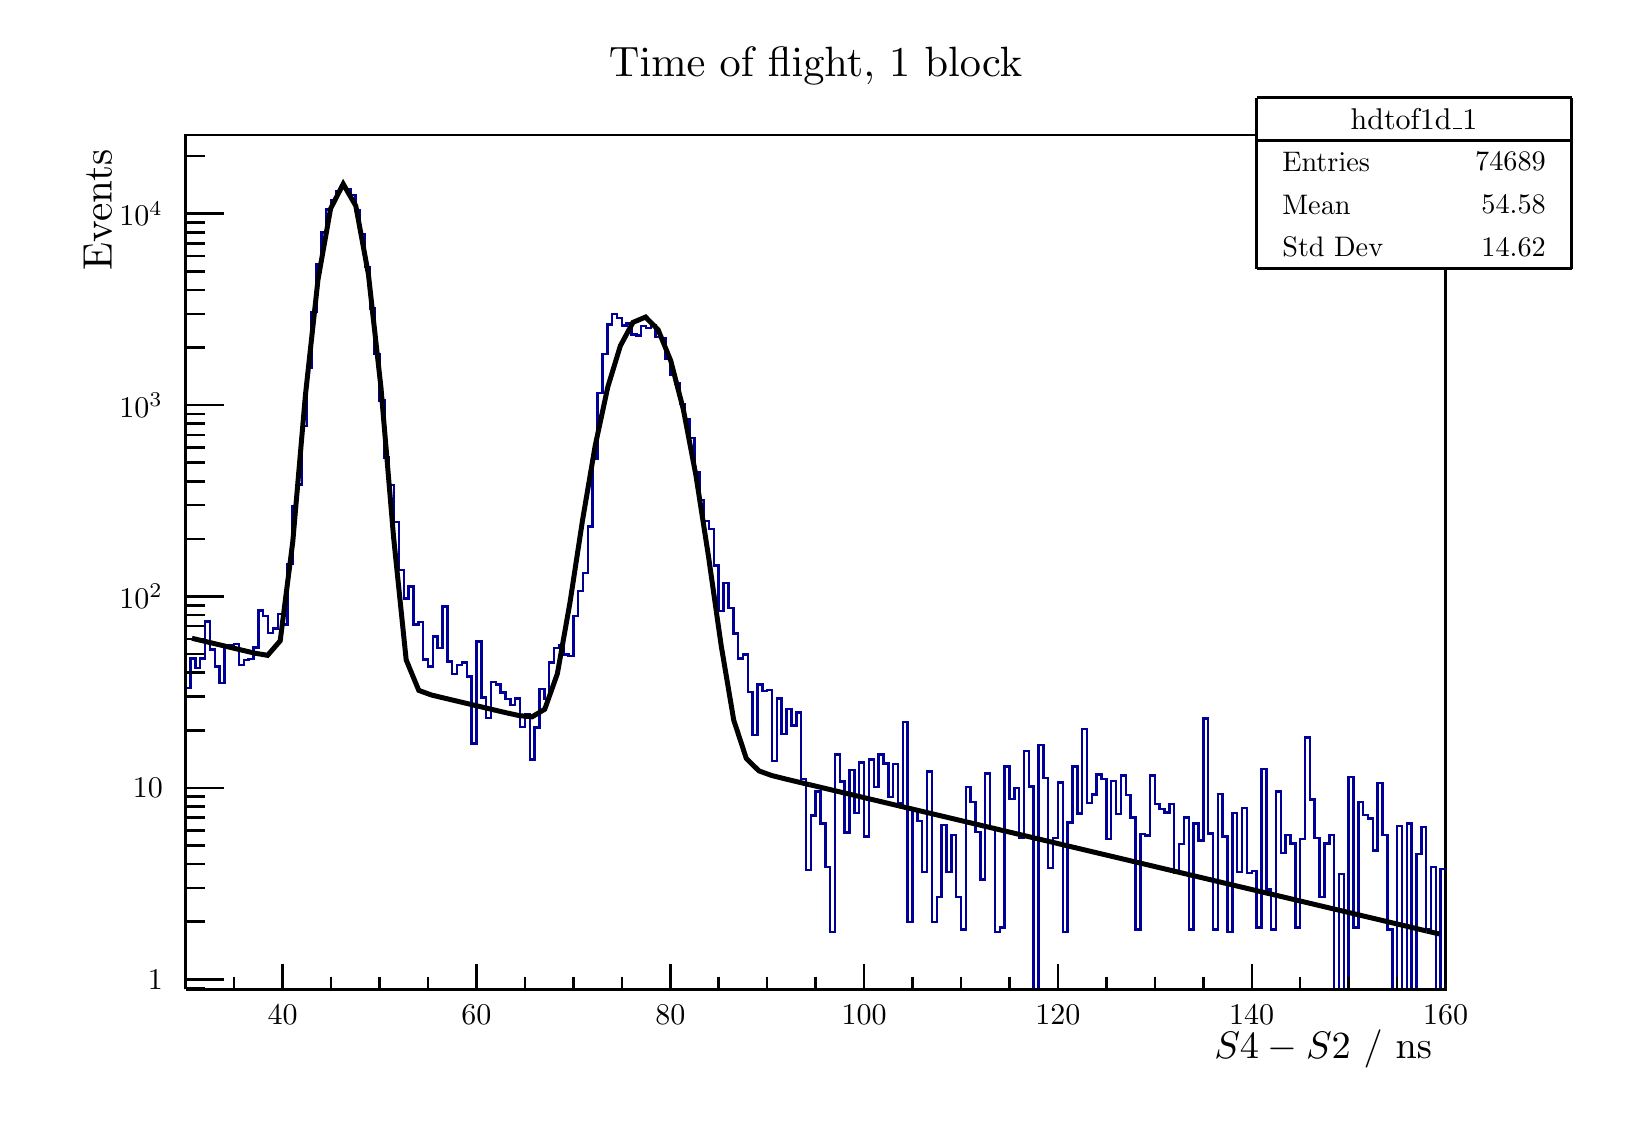
\begin{tikzpicture}
\pgfdeclareplotmark{cross} {
\pgfpathmoveto{\pgfpoint{-0.3\pgfplotmarksize}{\pgfplotmarksize}}
\pgfpathlineto{\pgfpoint{+0.3\pgfplotmarksize}{\pgfplotmarksize}}
\pgfpathlineto{\pgfpoint{+0.3\pgfplotmarksize}{0.3\pgfplotmarksize}}
\pgfpathlineto{\pgfpoint{+1\pgfplotmarksize}{0.3\pgfplotmarksize}}
\pgfpathlineto{\pgfpoint{+1\pgfplotmarksize}{-0.3\pgfplotmarksize}}
\pgfpathlineto{\pgfpoint{+0.3\pgfplotmarksize}{-0.3\pgfplotmarksize}}
\pgfpathlineto{\pgfpoint{+0.3\pgfplotmarksize}{-1.\pgfplotmarksize}}
\pgfpathlineto{\pgfpoint{-0.3\pgfplotmarksize}{-1.\pgfplotmarksize}}
\pgfpathlineto{\pgfpoint{-0.3\pgfplotmarksize}{-0.3\pgfplotmarksize}}
\pgfpathlineto{\pgfpoint{-1.\pgfplotmarksize}{-0.3\pgfplotmarksize}}
\pgfpathlineto{\pgfpoint{-1.\pgfplotmarksize}{0.3\pgfplotmarksize}}
\pgfpathlineto{\pgfpoint{-0.3\pgfplotmarksize}{0.3\pgfplotmarksize}}
\pgfpathclose
\pgfusepathqstroke
}
\pgfdeclareplotmark{cross*} {
\pgfpathmoveto{\pgfpoint{-0.3\pgfplotmarksize}{\pgfplotmarksize}}
\pgfpathlineto{\pgfpoint{+0.3\pgfplotmarksize}{\pgfplotmarksize}}
\pgfpathlineto{\pgfpoint{+0.3\pgfplotmarksize}{0.3\pgfplotmarksize}}
\pgfpathlineto{\pgfpoint{+1\pgfplotmarksize}{0.3\pgfplotmarksize}}
\pgfpathlineto{\pgfpoint{+1\pgfplotmarksize}{-0.3\pgfplotmarksize}}
\pgfpathlineto{\pgfpoint{+0.3\pgfplotmarksize}{-0.3\pgfplotmarksize}}
\pgfpathlineto{\pgfpoint{+0.3\pgfplotmarksize}{-1.\pgfplotmarksize}}
\pgfpathlineto{\pgfpoint{-0.3\pgfplotmarksize}{-1.\pgfplotmarksize}}
\pgfpathlineto{\pgfpoint{-0.3\pgfplotmarksize}{-0.3\pgfplotmarksize}}
\pgfpathlineto{\pgfpoint{-1.\pgfplotmarksize}{-0.3\pgfplotmarksize}}
\pgfpathlineto{\pgfpoint{-1.\pgfplotmarksize}{0.3\pgfplotmarksize}}
\pgfpathlineto{\pgfpoint{-0.3\pgfplotmarksize}{0.3\pgfplotmarksize}}
\pgfpathclose
\pgfusepathqfillstroke
}
\pgfdeclareplotmark{newstar} {
\pgfpathmoveto{\pgfqpoint{0pt}{\pgfplotmarksize}}
\pgfpathlineto{\pgfqpointpolar{44}{0.5\pgfplotmarksize}}
\pgfpathlineto{\pgfqpointpolar{18}{\pgfplotmarksize}}
\pgfpathlineto{\pgfqpointpolar{-20}{0.5\pgfplotmarksize}}
\pgfpathlineto{\pgfqpointpolar{-54}{\pgfplotmarksize}}
\pgfpathlineto{\pgfqpointpolar{-90}{0.5\pgfplotmarksize}}
\pgfpathlineto{\pgfqpointpolar{234}{\pgfplotmarksize}}
\pgfpathlineto{\pgfqpointpolar{198}{0.5\pgfplotmarksize}}
\pgfpathlineto{\pgfqpointpolar{162}{\pgfplotmarksize}}
\pgfpathlineto{\pgfqpointpolar{134}{0.5\pgfplotmarksize}}
\pgfpathclose
\pgfusepathqstroke
}
\pgfdeclareplotmark{newstar*} {
\pgfpathmoveto{\pgfqpoint{0pt}{\pgfplotmarksize}}
\pgfpathlineto{\pgfqpointpolar{44}{0.5\pgfplotmarksize}}
\pgfpathlineto{\pgfqpointpolar{18}{\pgfplotmarksize}}
\pgfpathlineto{\pgfqpointpolar{-20}{0.5\pgfplotmarksize}}
\pgfpathlineto{\pgfqpointpolar{-54}{\pgfplotmarksize}}
\pgfpathlineto{\pgfqpointpolar{-90}{0.5\pgfplotmarksize}}
\pgfpathlineto{\pgfqpointpolar{234}{\pgfplotmarksize}}
\pgfpathlineto{\pgfqpointpolar{198}{0.5\pgfplotmarksize}}
\pgfpathlineto{\pgfqpointpolar{162}{\pgfplotmarksize}}
\pgfpathlineto{\pgfqpointpolar{134}{0.5\pgfplotmarksize}}
\pgfpathclose
\pgfusepathqfillstroke
}
\definecolor{c}{rgb}{1,1,1};
\draw [color=c, fill=c] (0,0) rectangle (20,13.5632);
\draw [color=c, fill=c] (2,1.35632) rectangle (18,12.2069);
\definecolor{c}{rgb}{0,0,0};
\draw [c,line width=0.9] (2,1.35632) -- (2,12.2069) -- (18,12.2069) -- (18,1.35632) -- (2,1.35632);
\definecolor{c}{rgb}{1,1,1};
\draw [color=c, fill=c] (2,1.35632) rectangle (18,12.2069);
\definecolor{c}{rgb}{0,0,0};
\draw [c,line width=0.9] (2,1.35632) -- (2,12.2069) -- (18,12.2069) -- (18,1.35632) -- (2,1.35632);
\definecolor{c}{rgb}{0,0,0.6};
\draw [c,line width=0.9] (2,5.18151) -- (2.06154,5.18151) -- (2.06154,5.55608) -- (2.12308,5.55608) -- (2.12308,5.43961) -- (2.18462,5.43961) -- (2.18462,5.55581) -- (2.24615,5.55581) -- (2.24615,6.03099) -- (2.30769,6.03099) -- (2.30769,5.671) --
 (2.36923,5.671) -- (2.36923,5.45689) -- (2.43077,5.45689) -- (2.43077,5.24567) -- (2.49231,5.24567) -- (2.49231,5.73078) -- (2.55385,5.73078) -- (2.55385,5.72665) -- (2.61538,5.72665) -- (2.61538,5.74226) -- (2.67692,5.74226) -- (2.67692,5.47851) --
 (2.73846,5.47851) -- (2.73846,5.53808) -- (2.8,5.53808) -- (2.8,5.54976) -- (2.86154,5.54976) -- (2.86154,5.69856) -- (2.92308,5.69856) -- (2.92308,6.16999) -- (2.98462,6.16999) -- (2.98462,6.10032) -- (3.04615,6.10032) -- (3.04615,5.88449) --
 (3.10769,5.88449) -- (3.10769,5.93992) -- (3.16923,5.93992) -- (3.16923,6.12156) -- (3.23077,6.12156) -- (3.23077,5.99356) -- (3.29231,5.99356) -- (3.29231,6.75831) -- (3.35385,6.75831) -- (3.35385,7.49725) -- (3.41538,7.49725) -- (3.41538,7.76618)
 -- (3.47692,7.76618) -- (3.47692,8.5123) -- (3.53846,8.5123) -- (3.53846,9.25065) -- (3.6,9.25065) -- (3.6,9.95823) -- (3.66154,9.95823) -- (3.66154,10.5598) -- (3.72308,10.5598) -- (3.72308,10.9657) -- (3.78462,10.9657) -- (3.78462,11.2595) --
 (3.84615,11.2595) -- (3.84615,11.3826) -- (3.90769,11.3826) -- (3.90769,11.4937) -- (3.96923,11.4937) -- (3.96923,11.5322) -- (4.03077,11.5322) -- (4.03077,11.5125) -- (4.09231,11.5125) -- (4.09231,11.4476) -- (4.15385,11.4476) -- (4.15385,11.2503)
 -- (4.21538,11.2503) -- (4.21538,10.9505) -- (4.27692,10.9505) -- (4.27692,10.5305) -- (4.33846,10.5305) -- (4.33846,10.0019) -- (4.4,10.0019) -- (4.4,9.42602) -- (4.46154,9.42602) -- (4.46154,8.83371) -- (4.52308,8.83371) -- (4.52308,8.11005) --
 (4.58462,8.11005) -- (4.58462,7.76378) -- (4.64615,7.76378) -- (4.64615,7.29171) -- (4.70769,7.29171) -- (4.70769,6.67972) -- (4.76923,6.67972) -- (4.76923,6.32169) -- (4.83077,6.32169) -- (4.83077,6.47204) -- (4.89231,6.47204) -- (4.89231,5.993) --
 (4.95385,5.993) -- (4.95385,6.02017) -- (5.01538,6.02017) -- (5.01538,5.54748) -- (5.07692,5.54748) -- (5.07692,5.45714) -- (5.13846,5.45714) -- (5.13846,5.83864) -- (5.2,5.83864) -- (5.2,5.69096) -- (5.26154,5.69096) -- (5.26154,6.21606) --
 (5.32308,6.21606) -- (5.32308,5.51754) -- (5.38462,5.51754) -- (5.38462,5.35984) -- (5.44615,5.35984) -- (5.44615,5.47524) -- (5.50769,5.47524) -- (5.50769,5.50812) -- (5.56923,5.50812) -- (5.56923,5.32886) -- (5.63077,5.32886) -- (5.63077,4.47719)
 -- (5.69231,4.47719) -- (5.69231,5.77627) -- (5.75385,5.77627) -- (5.75385,5.06195) -- (5.81538,5.06195) -- (5.81538,4.80233) -- (5.87692,4.80233) -- (5.87692,5.25956) -- (5.93846,5.25956) -- (5.93846,5.22936) -- (6,5.22936) -- (6,5.12667) --
 (6.06154,5.12667) -- (6.06154,5.04604) -- (6.12308,5.04604) -- (6.12308,4.96718) -- (6.18462,4.96718) -- (6.18462,5.05252) -- (6.24615,5.05252) -- (6.24615,4.68623) -- (6.30769,4.68623) -- (6.30769,4.85157) -- (6.36923,4.85157) -- (6.36923,4.2741)
 -- (6.43077,4.2741) -- (6.43077,4.68523) -- (6.49231,4.68523) -- (6.49231,5.16964) -- (6.55385,5.16964) -- (6.55385,5.0443) -- (6.61538,5.0443) -- (6.61538,5.50863) -- (6.67692,5.50863) -- (6.67692,5.68975) -- (6.73846,5.68975) -- (6.73846,5.72166)
 -- (6.8,5.72166) -- (6.8,5.60763) -- (6.86154,5.60763) -- (6.86154,5.58722) -- (6.92308,5.58722) -- (6.92308,6.09935) -- (6.98462,6.09935) -- (6.98462,6.41753) -- (7.04615,6.41753) -- (7.04615,6.64659) -- (7.10769,6.64659) -- (7.10769,7.2355) --
 (7.16923,7.2355) -- (7.16923,8.09892) -- (7.23077,8.09892) -- (7.23077,8.93136) -- (7.29231,8.93136) -- (7.29231,9.42351) -- (7.35385,9.42351) -- (7.35385,9.79794) -- (7.41538,9.79794) -- (7.41538,9.93183) -- (7.47692,9.93183) -- (7.47692,9.8799) --
 (7.53846,9.8799) -- (7.53846,9.78722) -- (7.6,9.78722) -- (7.6,9.81608) -- (7.66154,9.81608) -- (7.66154,9.67331) -- (7.72308,9.67331) -- (7.72308,9.65902) -- (7.78462,9.65902) -- (7.78462,9.77948) -- (7.84615,9.77948) -- (7.84615,9.75876) --
 (7.90769,9.75876) -- (7.90769,9.79026) -- (7.96923,9.79026) -- (7.96923,9.64053) -- (8.03077,9.64053) -- (8.03077,9.63187) -- (8.09231,9.63187) -- (8.09231,9.36831) -- (8.15385,9.36831) -- (8.15385,9.16368) -- (8.21538,9.16368) -- (8.21538,9.05403)
 -- (8.27692,9.05403) -- (8.27692,8.78876) -- (8.33846,8.78876) -- (8.33846,8.603) -- (8.4,8.603) -- (8.4,8.35968) -- (8.46154,8.35968) -- (8.46154,7.91883) -- (8.52308,7.91883) -- (8.52308,7.56846) -- (8.58462,7.56846) -- (8.58462,7.30407) --
 (8.64615,7.30407) -- (8.64615,7.20532) -- (8.70769,7.20532) -- (8.70769,6.74177) -- (8.76923,6.74177) -- (8.76923,6.16352) -- (8.83077,6.16352) -- (8.83077,6.51821) -- (8.89231,6.51821) -- (8.89231,6.20221) -- (8.95385,6.20221) -- (8.95385,5.87638)
 -- (9.01538,5.87638) -- (9.01538,5.55625) -- (9.07692,5.55625) -- (9.07692,5.61066) -- (9.13846,5.61066) -- (9.13846,5.13328) -- (9.2,5.13328) -- (9.2,4.58783) -- (9.26154,4.58783) -- (9.26154,5.23012) -- (9.32308,5.23012) -- (9.32308,5.146) --
 (9.38461,5.146) -- (9.38461,5.15776) -- (9.44615,5.15776) -- (9.44615,4.25767) -- (9.50769,4.25767) -- (9.50769,5.04774) -- (9.56923,5.04774) -- (9.56923,4.60175) -- (9.63077,4.60175) -- (9.63077,4.92009) -- (9.69231,4.92009) -- (9.69231,4.71042) --
 (9.75385,4.71042) -- (9.75385,4.87061) -- (9.81538,4.87061) -- (9.81538,4.02592) -- (9.87692,4.02592) -- (9.87692,2.87449) -- (9.93846,2.87449) -- (9.93846,3.56693) -- (10,3.56693) -- (10,3.87246) -- (10.0615,3.87246) -- (10.0615,3.4613) --
 (10.1231,3.4613) -- (10.1231,2.90853) -- (10.1846,2.90853) -- (10.1846,2.08809) -- (10.2462,2.08809) -- (10.2462,4.33668) -- (10.3077,4.33668) -- (10.3077,3.99697) -- (10.3692,3.99697) -- (10.3692,3.3477) -- (10.4308,3.3477) -- (10.4308,4.13973) --
 (10.4923,4.13973) -- (10.4923,3.59781) -- (10.5538,3.59781) -- (10.5538,4.23774) -- (10.6154,4.23774) -- (10.6154,3.29987) -- (10.6769,3.29987) -- (10.6769,4.27622) -- (10.7385,4.27622) -- (10.7385,3.92545) -- (10.8,3.92545) -- (10.8,4.34213) --
 (10.8615,4.34213) -- (10.8615,4.22691) -- (10.9231,4.22691) -- (10.9231,3.79686) -- (10.9846,3.79686) -- (10.9846,4.22057) -- (11.0462,4.22057) -- (11.0462,3.71905) -- (11.1077,3.71905) -- (11.1077,4.75094) -- (11.1692,4.75094) -- (11.1692,2.20974)
 -- (11.2308,2.20974) -- (11.2308,3.65017) -- (11.2923,3.65017) -- (11.2923,3.492) -- (11.3538,3.492) -- (11.3538,2.84753) -- (11.4154,2.84753) -- (11.4154,4.12337) -- (11.4769,4.12337) -- (11.4769,2.20974) -- (11.5385,2.20974) -- (11.5385,2.53059)
 -- (11.6,2.53059) -- (11.6,3.44296) -- (11.6615,3.44296) -- (11.6615,2.84753) -- (11.7231,2.84753) -- (11.7231,3.31942) -- (11.7846,3.31942) -- (11.7846,2.53059) -- (11.8462,2.53059) -- (11.8462,2.11846) -- (11.9077,2.11846) -- (11.9077,3.92545) --
 (11.9692,3.92545) -- (11.9692,3.73625) -- (12.0308,3.73625) -- (12.0308,3.35377) -- (12.0923,3.35377) -- (12.0923,2.74928) -- (12.1538,2.74928) -- (12.1538,4.09554) -- (12.2154,4.09554) -- (12.2154,3.41687) -- (12.2769,3.41687) -- (12.2769,2.08809)
 -- (12.3385,2.08809) -- (12.3385,2.14272) -- (12.4,2.14272) -- (12.4,4.18641) -- (12.4615,4.18641) -- (12.4615,3.77723) -- (12.5231,3.77723) -- (12.5231,3.91398) -- (12.5846,3.91398) -- (12.5846,3.27829) -- (12.6462,3.27829) -- (12.6462,4.38363) --
 (12.7077,4.38363) -- (12.7077,3.93124) -- (12.7692,3.93124) -- (12.7692,1.35632) -- (12.8308,1.35632) -- (12.8308,4.45728) -- (12.8923,4.45728) -- (12.8923,4.04146) -- (12.9538,4.04146) -- (12.9538,2.89686) -- (13.0154,2.89686) -- (13.0154,3.27649)
 -- (13.0769,3.27649) -- (13.0769,3.98168) -- (13.1385,3.98168) -- (13.1385,2.08809) -- (13.2,2.08809) -- (13.2,3.47404) -- (13.2615,3.47404) -- (13.2615,4.18641) -- (13.3231,4.18641) -- (13.3231,3.58812) -- (13.3846,3.58812) -- (13.3846,4.66074) --
 (13.4462,4.66074) -- (13.4462,3.72096) -- (13.5077,3.72096) -- (13.5077,3.83058) -- (13.5692,3.83058) -- (13.5692,4.08766) -- (13.6308,4.08766) -- (13.6308,4.03023) -- (13.6923,4.03023) -- (13.6923,3.26645) -- (13.7538,3.26645) -- (13.7538,4.00415)
 -- (13.8154,4.00415) -- (13.8154,3.58678) -- (13.8769,3.58678) -- (13.8769,4.07563) -- (13.9385,4.07563) -- (13.9385,3.82377) -- (14,3.82377) -- (14,3.53914) -- (14.0615,3.53914) -- (14.0615,2.11846) -- (14.1231,2.11846) -- (14.1231,3.33056) --
 (14.1846,3.33056) -- (14.1846,3.3096) -- (14.2462,3.3096) -- (14.2462,4.07579) -- (14.3077,4.07579) -- (14.3077,3.70785) -- (14.3692,3.70785) -- (14.3692,3.64917) -- (14.4308,3.64917) -- (14.4308,3.60516) -- (14.4923,3.60516) -- (14.4923,3.70785) --
 (14.5538,3.70785) -- (14.5538,2.83516) -- (14.6154,2.83516) -- (14.6154,3.20139) -- (14.6769,3.20139) -- (14.6769,3.53914) -- (14.7385,3.53914) -- (14.7385,2.11846) -- (14.8,2.11846) -- (14.8,3.46572) -- (14.8615,3.46572) -- (14.8615,3.24538) --
 (14.9231,3.24538) -- (14.9231,4.79484) -- (14.9846,4.79484) -- (14.9846,3.33729) -- (15.0462,3.33729) -- (15.0462,2.11846) -- (15.1077,2.11846) -- (15.1077,3.83614) -- (15.1692,3.83614) -- (15.1692,3.29647) -- (15.2308,3.29647) -- (15.2308,2.08809)
 -- (15.2923,2.08809) -- (15.2923,3.59713) -- (15.3538,3.59713) -- (15.3538,2.85023) -- (15.4154,2.85023) -- (15.4154,3.66286) -- (15.4769,3.66286) -- (15.4769,2.83516) -- (15.5385,2.83516) -- (15.5385,2.86243) -- (15.6,2.86243) -- (15.6,2.14272) --
 (15.6615,2.14272) -- (15.6615,4.15383) -- (15.7231,4.15383) -- (15.7231,2.62199) -- (15.7846,2.62199) -- (15.7846,2.11846) -- (15.8462,2.11846) -- (15.8462,3.87165) -- (15.9077,3.87165) -- (15.9077,3.08614) -- (15.9692,3.08614) -- (15.9692,3.31751)
 -- (16.0308,3.31751) -- (16.0308,3.21207) -- (16.0923,3.21207) -- (16.0923,2.14272) -- (16.1538,2.14272) -- (16.1538,3.26826) -- (16.2154,3.26826) -- (16.2154,4.55325) -- (16.2769,4.55325) -- (16.2769,3.77087) -- (16.3385,3.77087) --
 (16.3385,3.27829) -- (16.4,3.27829) -- (16.4,2.53059) -- (16.4615,2.53059) -- (16.4615,3.21207) -- (16.5231,3.21207) -- (16.5231,3.31751) -- (16.5846,3.31751) -- (16.5846,1.35632) -- (16.6462,1.35632) -- (16.6462,2.81986) -- (16.7077,2.81986) --
 (16.7077,1.35632) -- (16.7692,1.35632) -- (16.7692,4.05445) -- (16.8308,4.05445) -- (16.8308,2.14272) -- (16.8923,2.14272) -- (16.8923,3.7376) -- (16.9538,3.7376) -- (16.9538,3.57313) -- (17.0154,3.57313) -- (17.0154,3.52486) -- (17.0769,3.52486) --
 (17.0769,3.12021) -- (17.1385,3.12021) -- (17.1385,3.98035) -- (17.2,3.98035) -- (17.2,3.31751) -- (17.2615,3.31751) -- (17.2615,2.11846) -- (17.3231,2.11846) -- (17.3231,1.35632) -- (17.3846,1.35632) -- (17.3846,3.43423) -- (17.4462,3.43423) --
 (17.4462,1.35632) -- (17.5077,1.35632) -- (17.5077,3.4613) -- (17.5692,3.4613) -- (17.5692,1.35632) -- (17.6308,1.35632) -- (17.6308,3.07628) -- (17.6923,3.07628) -- (17.6923,3.41932) -- (17.7538,3.41932) -- (17.7538,2.11846) -- (17.8154,2.11846) --
 (17.8154,2.90853) -- (17.8769,2.90853) -- (17.8769,1.35632) -- (17.9385,1.35632) -- (17.9385,2.88244) -- (18,2.88244);
\definecolor{c}{rgb}{0,0,0};
\draw [c,line width=0.9] (2,1.35632) -- (18,1.35632);
\draw [anchor= east] (18,0.596782) node[scale=1.38496, color=c, rotate=0]{$S4 - S2$ / ns};
\draw [c,line width=0.9] (3.23077,1.68184) -- (3.23077,1.35632);
\draw [c,line width=0.9] (3.84615,1.51908) -- (3.84615,1.35632);
\draw [c,line width=0.9] (4.46154,1.51908) -- (4.46154,1.35632);
\draw [c,line width=0.9] (5.07692,1.51908) -- (5.07692,1.35632);
\draw [c,line width=0.9] (5.69231,1.68184) -- (5.69231,1.35632);
\draw [c,line width=0.9] (6.30769,1.51908) -- (6.30769,1.35632);
\draw [c,line width=0.9] (6.92308,1.51908) -- (6.92308,1.35632);
\draw [c,line width=0.9] (7.53846,1.51908) -- (7.53846,1.35632);
\draw [c,line width=0.9] (8.15385,1.68184) -- (8.15385,1.35632);
\draw [c,line width=0.9] (8.76923,1.51908) -- (8.76923,1.35632);
\draw [c,line width=0.9] (9.38461,1.51908) -- (9.38461,1.35632);
\draw [c,line width=0.9] (10,1.51908) -- (10,1.35632);
\draw [c,line width=0.9] (10.6154,1.68184) -- (10.6154,1.35632);
\draw [c,line width=0.9] (11.2308,1.51908) -- (11.2308,1.35632);
\draw [c,line width=0.9] (11.8462,1.51908) -- (11.8462,1.35632);
\draw [c,line width=0.9] (12.4615,1.51908) -- (12.4615,1.35632);
\draw [c,line width=0.9] (13.0769,1.68184) -- (13.0769,1.35632);
\draw [c,line width=0.9] (13.6923,1.51908) -- (13.6923,1.35632);
\draw [c,line width=0.9] (14.3077,1.51908) -- (14.3077,1.35632);
\draw [c,line width=0.9] (14.9231,1.51908) -- (14.9231,1.35632);
\draw [c,line width=0.9] (15.5385,1.68184) -- (15.5385,1.35632);
\draw [c,line width=0.9] (16.1538,1.51908) -- (16.1538,1.35632);
\draw [c,line width=0.9] (16.7692,1.51908) -- (16.7692,1.35632);
\draw [c,line width=0.9] (17.3846,1.51908) -- (17.3846,1.35632);
\draw [c,line width=0.9] (18,1.68184) -- (18,1.35632);
\draw [c,line width=0.9] (3.23077,1.68184) -- (3.23077,1.35632);
\draw [c,line width=0.9] (2.61538,1.51908) -- (2.61538,1.35632);
\draw [c,line width=0.9] (2,1.51908) -- (2,1.35632);
\draw [anchor=base] (3.23077,0.908736) node[scale=1.08496, color=c, rotate=0]{40};
\draw [anchor=base] (5.69231,0.908736) node[scale=1.08496, color=c, rotate=0]{60};
\draw [anchor=base] (8.15385,0.908736) node[scale=1.08496, color=c, rotate=0]{80};
\draw [anchor=base] (10.6154,0.908736) node[scale=1.08496, color=c, rotate=0]{100};
\draw [anchor=base] (13.0769,0.908736) node[scale=1.08496, color=c, rotate=0]{120};
\draw [anchor=base] (15.5385,0.908736) node[scale=1.08496, color=c, rotate=0]{140};
\draw [anchor=base] (18,0.908736) node[scale=1.08496, color=c, rotate=0]{160};
\draw [c,line width=0.9] (2,1.35632) -- (2,12.2069);
\draw [anchor= east] (0.88,12.2069) node[scale=1.48496, color=c, rotate=90]{ Events};
\draw [c,line width=0.9] (2.24,1.37274) -- (2,1.37274);
\draw [c,line width=0.9] (2.48,1.48397) -- (2,1.48397);
\draw [anchor= east] (1.844,1.48397) node[scale=1.08496, color=c, rotate=0]{1};
\draw [c,line width=0.9] (2.24,2.21574) -- (2,2.21574);
\draw [c,line width=0.9] (2.24,2.6438) -- (2,2.6438);
\draw [c,line width=0.9] (2.24,2.94751) -- (2,2.94751);
\draw [c,line width=0.9] (2.24,3.18309) -- (2,3.18309);
\draw [c,line width=0.9] (2.24,3.37557) -- (2,3.37557);
\draw [c,line width=0.9] (2.24,3.53831) -- (2,3.53831);
\draw [c,line width=0.9] (2.24,3.67928) -- (2,3.67928);
\draw [c,line width=0.9] (2.24,3.80363) -- (2,3.80363);
\draw [c,line width=0.9] (2.48,3.91486) -- (2,3.91486);
\draw [anchor= east] (1.844,3.91486) node[scale=1.08496, color=c, rotate=0]{10};
\draw [c,line width=0.9] (2.24,4.64663) -- (2,4.64663);
\draw [c,line width=0.9] (2.24,5.07469) -- (2,5.07469);
\draw [c,line width=0.9] (2.24,5.3784) -- (2,5.3784);
\draw [c,line width=0.9] (2.24,5.61398) -- (2,5.61398);
\draw [c,line width=0.9] (2.24,5.80646) -- (2,5.80646);
\draw [c,line width=0.9] (2.24,5.9692) -- (2,5.9692);
\draw [c,line width=0.9] (2.24,6.11017) -- (2,6.11017);
\draw [c,line width=0.9] (2.24,6.23452) -- (2,6.23452);
\draw [c,line width=0.9] (2.48,6.34575) -- (2,6.34575);
\draw [anchor= east] (1.844,6.34575) node[scale=1.08496, color=c, rotate=0]{$10^{2}$};
\draw [c,line width=0.9] (2.24,7.07752) -- (2,7.07752);
\draw [c,line width=0.9] (2.24,7.50558) -- (2,7.50558);
\draw [c,line width=0.9] (2.24,7.80929) -- (2,7.80929);
\draw [c,line width=0.9] (2.24,8.04487) -- (2,8.04487);
\draw [c,line width=0.9] (2.24,8.23735) -- (2,8.23735);
\draw [c,line width=0.9] (2.24,8.40009) -- (2,8.40009);
\draw [c,line width=0.9] (2.24,8.54106) -- (2,8.54106);
\draw [c,line width=0.9] (2.24,8.66541) -- (2,8.66541);
\draw [c,line width=0.9] (2.48,8.77664) -- (2,8.77664);
\draw [anchor= east] (1.844,8.77664) node[scale=1.08496, color=c, rotate=0]{$10^{3}$};
\draw [c,line width=0.9] (2.24,9.50841) -- (2,9.50841);
\draw [c,line width=0.9] (2.24,9.93647) -- (2,9.93647);
\draw [c,line width=0.9] (2.24,10.2402) -- (2,10.2402);
\draw [c,line width=0.9] (2.24,10.4758) -- (2,10.4758);
\draw [c,line width=0.9] (2.24,10.6682) -- (2,10.6682);
\draw [c,line width=0.9] (2.24,10.831) -- (2,10.831);
\draw [c,line width=0.9] (2.24,10.9719) -- (2,10.9719);
\draw [c,line width=0.9] (2.24,11.0963) -- (2,11.0963);
\draw [c,line width=0.9] (2.48,11.2075) -- (2,11.2075);
\draw [anchor= east] (1.844,11.2075) node[scale=1.08496, color=c, rotate=0]{$10^{4}$};
\draw [c,line width=0.9] (2.24,11.9393) -- (2,11.9393);
\definecolor{c}{rgb}{1,1,1};
\draw [color=c, fill=c] (15.6,10.5115) rectangle (19.6,12.6816);
\definecolor{c}{rgb}{0,0,0};
\draw [c,line width=0.9] (15.6,10.5115) -- (19.6,10.5115);
\draw [c,line width=0.9] (19.6,10.5115) -- (19.6,12.6816);
\draw [c,line width=0.9] (19.6,12.6816) -- (15.6,12.6816);
\draw [c,line width=0.9] (15.6,12.6816) -- (15.6,10.5115);
\draw (17.6,12.4103) node[scale=1.08496, color=c, rotate=0]{hdtof1d\_1};
\draw [c,line width=0.9] (15.6,12.1391) -- (19.6,12.1391);
\draw [anchor= west] (15.8,11.8678) node[scale=1.02114, color=c, rotate=0]{Entries };
\draw [anchor= east] (19.4,11.8678) node[scale=1.02114, color=c, rotate=0]{ 74689};
\draw [anchor= west] (15.8,11.3253) node[scale=1.02114, color=c, rotate=0]{Mean  };
\draw [anchor= east] (19.4,11.3253) node[scale=1.02114, color=c, rotate=0]{  54.58};
\draw [anchor= west] (15.8,10.7828) node[scale=1.02114, color=c, rotate=0]{Std Dev   };
\draw [anchor= east] (19.4,10.7828) node[scale=1.02114, color=c, rotate=0]{  14.62};
\draw [c,line width=1.8] (2.08,5.81522) -- (2.24,5.77729) -- (2.4,5.73936) -- (2.56,5.70143) -- (2.72,5.6635) -- (2.88,5.62584) -- (3.04,5.59883) -- (3.2,5.783) -- (3.36,7.04462) -- (3.52,8.89992) -- (3.68,10.3694) -- (3.84,11.2716) -- (4,11.5852) --
 (4.16,11.3072) -- (4.32,10.4394) -- (4.48,8.9965) -- (4.64,7.0994) -- (4.8,5.54055) -- (4.96,5.1535) -- (5.12,5.09513) -- (5.28,5.05662) -- (5.44,5.01869) -- (5.6,4.98076) -- (5.76,4.94283) -- (5.92,4.90492) -- (6.08,4.86731) -- (6.24,4.83246) --
 (6.4,4.81808) -- (6.56,4.91497) -- (6.72,5.3653) -- (6.88,6.26787) -- (7.04,7.31709) -- (7.2,8.25867) -- (7.36,9.00435) -- (7.52,9.52953) -- (7.68,9.82711) -- (7.84,9.89492) -- (8,9.73249) -- (8.16,9.34039) -- (8.32,8.721) -- (8.48,7.88215) --
 (8.64,6.85117) -- (8.8,5.72561) -- (8.96,4.77556) -- (9.12,4.2879) -- (9.28,4.13137) -- (9.44,4.0733) -- (9.6,4.03279) -- (9.76,3.9946) -- (9.92,3.95665);
\draw [c,line width=1.8] (9.92,3.95665) -- (10.08,3.91871) -- (10.24,3.88078) -- (10.4,3.84285) -- (10.56,3.80492) -- (10.72,3.76699) -- (10.88,3.72906) -- (11.04,3.69113) -- (11.2,3.6532) -- (11.36,3.61527) -- (11.52,3.57734) -- (11.68,3.53941) --
 (11.84,3.50148) -- (12,3.46355) -- (12.16,3.42562) -- (12.32,3.38769) -- (12.48,3.34976) -- (12.64,3.31183) -- (12.8,3.2739) -- (12.96,3.23597) -- (13.12,3.19804) -- (13.28,3.16011) -- (13.44,3.12218) -- (13.6,3.08425) -- (13.76,3.04632) --
 (13.92,3.00839) -- (14.08,2.97046) -- (14.24,2.93253) -- (14.4,2.8946) -- (14.56,2.85667) -- (14.72,2.81874) -- (14.88,2.78081) -- (15.04,2.74288) -- (15.2,2.70495) -- (15.36,2.66702) -- (15.52,2.62909) -- (15.68,2.59116) -- (15.84,2.55323) --
 (16,2.5153) -- (16.16,2.47737) -- (16.32,2.43944) -- (16.48,2.40151) -- (16.64,2.36358) -- (16.8,2.32565) -- (16.96,2.28772) -- (17.12,2.24979) -- (17.28,2.21186) -- (17.44,2.17393) -- (17.6,2.136) -- (17.76,2.09807);
\draw [c,line width=1.8] (17.76,2.09807) -- (17.92,2.06014);
\draw (10,13.0816) node[scale=1.5317, color=c, rotate=0]{Time of flight, 1 block};
\end{tikzpicture}

  \end{adjustbox}
  \caption{Example of the time of flight spectrum observed in $\mathit{S4}$ with a combined signal and background function fitted (shown in black)}
  \label{fig:fitEx}
\end{figure}

To produce the data used in this analysis, an exponential background function is subtracted. 
The parameters for this function are taken from the combined signal and background function.


